\documentclass[twoside]{book}

% Packages required by doxygen
\usepackage{fixltx2e}
\usepackage{calc}
\usepackage{doxygen}
\usepackage[export]{adjustbox} % also loads graphicx
\usepackage{graphicx}
\usepackage[utf8]{inputenc}
\usepackage{makeidx}
\usepackage{multicol}
\usepackage{multirow}
\PassOptionsToPackage{warn}{textcomp}
\usepackage{textcomp}
\usepackage[nointegrals]{wasysym}
\usepackage[table]{xcolor}

% Font selection
\usepackage[T1]{fontenc}
\usepackage[scaled=.90]{helvet}
\usepackage{courier}
\usepackage{amssymb}
\usepackage{sectsty}
\renewcommand{\familydefault}{\sfdefault}
\allsectionsfont{%
  \fontseries{bc}\selectfont%
  \color{darkgray}%
}
\renewcommand{\DoxyLabelFont}{%
  \fontseries{bc}\selectfont%
  \color{darkgray}%
}
\newcommand{\+}{\discretionary{\mbox{\scriptsize$\hookleftarrow$}}{}{}}

% Page & text layout
\usepackage{geometry}
\geometry{%
  a4paper,%
  top=2.5cm,%
  bottom=2.5cm,%
  left=2.5cm,%
  right=2.5cm%
}
\tolerance=750
\hfuzz=15pt
\hbadness=750
\setlength{\emergencystretch}{15pt}
\setlength{\parindent}{0cm}
\setlength{\parskip}{3ex plus 2ex minus 2ex}
\makeatletter
\renewcommand{\paragraph}{%
  \@startsection{paragraph}{4}{0ex}{-1.0ex}{1.0ex}{%
    \normalfont\normalsize\bfseries\SS@parafont%
  }%
}
\renewcommand{\subparagraph}{%
  \@startsection{subparagraph}{5}{0ex}{-1.0ex}{1.0ex}{%
    \normalfont\normalsize\bfseries\SS@subparafont%
  }%
}
\makeatother

% Headers & footers
\usepackage{fancyhdr}
\pagestyle{fancyplain}
\fancyhead[LE]{\fancyplain{}{\bfseries\thepage}}
\fancyhead[CE]{\fancyplain{}{}}
\fancyhead[RE]{\fancyplain{}{\bfseries\leftmark}}
\fancyhead[LO]{\fancyplain{}{\bfseries\rightmark}}
\fancyhead[CO]{\fancyplain{}{}}
\fancyhead[RO]{\fancyplain{}{\bfseries\thepage}}
\fancyfoot[LE]{\fancyplain{}{}}
\fancyfoot[CE]{\fancyplain{}{}}
\fancyfoot[RE]{\fancyplain{}{\bfseries\scriptsize Generated by Doxygen }}
\fancyfoot[LO]{\fancyplain{}{\bfseries\scriptsize Generated by Doxygen }}
\fancyfoot[CO]{\fancyplain{}{}}
\fancyfoot[RO]{\fancyplain{}{}}
\renewcommand{\footrulewidth}{0.4pt}
\renewcommand{\chaptermark}[1]{%
  \markboth{#1}{}%
}
\renewcommand{\sectionmark}[1]{%
  \markright{\thesection\ #1}%
}

% Indices & bibliography
\usepackage{natbib}
\usepackage[titles]{tocloft}
\setcounter{tocdepth}{3}
\setcounter{secnumdepth}{5}
\makeindex

% Hyperlinks (required, but should be loaded last)
\usepackage{ifpdf}
\ifpdf
  \usepackage[pdftex,pagebackref=true]{hyperref}
\else
  \usepackage[ps2pdf,pagebackref=true]{hyperref}
\fi
\hypersetup{%
  colorlinks=true,%
  linkcolor=blue,%
  citecolor=blue,%
  unicode%
}

% Custom commands
\newcommand{\clearemptydoublepage}{%
  \newpage{\pagestyle{empty}\cleardoublepage}%
}

\usepackage{caption}
\captionsetup{labelsep=space,justification=centering,font={bf},singlelinecheck=off,skip=4pt,position=top}

%===== C O N T E N T S =====

\begin{document}

% Titlepage & ToC
\hypersetup{pageanchor=false,
             bookmarksnumbered=true,
             pdfencoding=unicode
            }
\pagenumbering{alph}
\begin{titlepage}
\vspace*{7cm}
\begin{center}%
{\Large S\+U\+E\+W\+S-\/\+An\+O\+HM \\[1ex]\large 0.\+9 }\\
\vspace*{1cm}
{\large Generated by Doxygen 1.8.13}\\
\end{center}
\end{titlepage}
\clearemptydoublepage
\pagenumbering{roman}
\tableofcontents
\clearemptydoublepage
\pagenumbering{arabic}
\hypersetup{pageanchor=true}

%--- Begin generated contents ---
\chapter{R\+E\+A\+D\+ME}
\label{md__r_e_a_d_m_e}
\Hypertarget{md__r_e_a_d_m_e}
Coding Guidelines \href{http://urban-climate.net/umep/DevelopmentGuidelines#Coding_Guidelines%7C}{\tt http\+://urban-\/climate.\+net/umep/\+Development\+Guidelines\#\+Coding\+\_\+\+Guidelines\%7C}

Manual \href{http://urban-climate.net/umep/SUEWS}{\tt http\+://urban-\/climate.\+net/umep/\+S\+U\+E\+WS}

\subsection*{Actions needed}

Benchmark data for testind developments

\subsubsection*{What is this repository for?}


\begin{DoxyItemize}
\item Quick summary
\item Version
\item \href{https://bitbucket.org/tutorials/markdowndemo}{\tt Learn Markdown}
\end{DoxyItemize}

\subsubsection*{How do I get set up?}


\begin{DoxyItemize}
\item Summary of set up
\item Configuration
\item Dependencies
\item Database configuration
\item How to run tests
\item Deployment instructions
\end{DoxyItemize}

\subsubsection*{Contribution guidelines}


\begin{DoxyItemize}
\item Writing tests
\item Code review
\item Other guidelines
\end{DoxyItemize}

\subsubsection*{Who do I talk to?}


\begin{DoxyItemize}
\item Repo owner or admin
\item Other community or team contact 
\end{DoxyItemize}
\chapter{Modules Index}
\section{Modules List}
Here is a list of all modules with brief descriptions\+:\begin{DoxyCompactList}
\item\contentsline{section}{\hyperlink{namespaceallocatearray}{allocatearray} }{\pageref{namespaceallocatearray}}{}
\item\contentsline{section}{\hyperlink{namespaceanohm__module}{anohm\+\_\+module} \\*An\+O\+HM\+: Analytical Objective Hysteresis Model }{\pageref{namespaceanohm__module}}{}
\item\contentsline{section}{\hyperlink{namespacecbl__module}{cbl\+\_\+module} }{\pageref{namespacecbl__module}}{}
\item\contentsline{section}{\hyperlink{namespacecolnamesinputfiles}{colnamesinputfiles} }{\pageref{namespacecolnamesinputfiles}}{}
\item\contentsline{section}{\hyperlink{namespacecolnamesmodeldailystate}{colnamesmodeldailystate} }{\pageref{namespacecolnamesmodeldailystate}}{}
\item\contentsline{section}{\hyperlink{namespacectrl__output}{ctrl\+\_\+output} }{\pageref{namespacectrl__output}}{}
\item\contentsline{section}{\hyperlink{namespacedata__in}{data\+\_\+in} }{\pageref{namespacedata__in}}{}
\item\contentsline{section}{\hyperlink{namespacedefaultnotused}{defaultnotused} }{\pageref{namespacedefaultnotused}}{}
\item\contentsline{section}{\hyperlink{namespaceestm__data}{estm\+\_\+data} }{\pageref{namespaceestm__data}}{}
\item\contentsline{section}{\hyperlink{namespacefilename}{filename} }{\pageref{namespacefilename}}{}
\item\contentsline{section}{\hyperlink{namespacegas}{gas} }{\pageref{namespacegas}}{}
\item\contentsline{section}{\hyperlink{namespacegis__data}{gis\+\_\+data} }{\pageref{namespacegis__data}}{}
\item\contentsline{section}{\hyperlink{namespaceheatflux}{heatflux} }{\pageref{namespaceheatflux}}{}
\item\contentsline{section}{\hyperlink{namespaceinitial}{initial} }{\pageref{namespaceinitial}}{}
\item\contentsline{section}{\hyperlink{namespaceinitialcond}{initialcond} }{\pageref{namespaceinitialcond}}{}
\item\contentsline{section}{\hyperlink{namespacemathconstants}{mathconstants} }{\pageref{namespacemathconstants}}{}
\item\contentsline{section}{\hyperlink{namespacematsize}{matsize} }{\pageref{namespacematsize}}{}
\item\contentsline{section}{\hyperlink{namespacemetdisagg}{metdisagg} }{\pageref{namespacemetdisagg}}{}
\item\contentsline{section}{\hyperlink{namespacemeteo}{meteo} }{\pageref{namespacemeteo}}{}
\item\contentsline{section}{\hyperlink{namespacemod__grav}{mod\+\_\+grav} }{\pageref{namespacemod__grav}}{}
\item\contentsline{section}{\hyperlink{namespacemod__interp}{mod\+\_\+interp} }{\pageref{namespacemod__interp}}{}
\item\contentsline{section}{\hyperlink{namespacemod__k}{mod\+\_\+k} }{\pageref{namespacemod__k}}{}
\item\contentsline{section}{\hyperlink{namespacemod__solver}{mod\+\_\+solver} }{\pageref{namespacemod__solver}}{}
\item\contentsline{section}{\hyperlink{namespacemod__z}{mod\+\_\+z} }{\pageref{namespacemod__z}}{}
\item\contentsline{section}{\hyperlink{namespacemodsolarcalc}{modsolarcalc} }{\pageref{namespacemodsolarcalc}}{}
\item\contentsline{section}{\hyperlink{namespacemoist}{moist} }{\pageref{namespacemoist}}{}
\item\contentsline{section}{\hyperlink{namespacenarp__module}{narp\+\_\+module} }{\pageref{namespacenarp__module}}{}
\item\contentsline{section}{\hyperlink{namespacephysconstants}{physconstants} }{\pageref{namespacephysconstants}}{}
\item\contentsline{section}{\hyperlink{namespaceprecision}{precision} }{\pageref{namespaceprecision}}{}
\item\contentsline{section}{\hyperlink{namespaceqsort__c__module}{qsort\+\_\+c\+\_\+module} }{\pageref{namespaceqsort__c__module}}{}
\item\contentsline{section}{\hyperlink{namespaceresist}{resist} }{\pageref{namespaceresist}}{}
\item\contentsline{section}{\hyperlink{namespacerun__info}{run\+\_\+info} }{\pageref{namespacerun__info}}{}
\item\contentsline{section}{\hyperlink{namespacesnowmod}{snowmod} }{\pageref{namespacesnowmod}}{}
\item\contentsline{section}{\hyperlink{namespacesolweig__module}{solweig\+\_\+module} }{\pageref{namespacesolweig__module}}{}
\item\contentsline{section}{\hyperlink{namespacestrings}{strings} }{\pageref{namespacestrings}}{}
\item\contentsline{section}{\hyperlink{namespacesues__data}{sues\+\_\+data} }{\pageref{namespacesues__data}}{}
\item\contentsline{section}{\hyperlink{namespacethresh}{thresh} }{\pageref{namespacethresh}}{}
\item\contentsline{section}{\hyperlink{namespacetime}{time} }{\pageref{namespacetime}}{}
\item\contentsline{section}{\hyperlink{namespacevegphenogy}{vegphenogy} }{\pageref{namespacevegphenogy}}{}
\item\contentsline{section}{\hyperlink{namespacewherewhen}{wherewhen} }{\pageref{namespacewherewhen}}{}
\end{DoxyCompactList}

\chapter{Data Type Index}
\section{Data Types List}
Here are the data types with brief descriptions\+:\begin{DoxyCompactList}
\item\contentsline{section}{\hyperlink{interfacestrings_1_1value}{strings\+::value} }{\pageref{interfacestrings_1_1value}}{}
\item\contentsline{section}{\hyperlink{structctrl__output_1_1varattr}{ctrl\+\_\+output\+::varattr} }{\pageref{structctrl__output_1_1varattr}}{}
\item\contentsline{section}{\hyperlink{interfacestrings_1_1writenum}{strings\+::writenum} }{\pageref{interfacestrings_1_1writenum}}{}
\item\contentsline{section}{\hyperlink{interfacestrings_1_1writeq}{strings\+::writeq} }{\pageref{interfacestrings_1_1writeq}}{}
\end{DoxyCompactList}

\chapter{File Index}
\section{File List}
Here is a list of all files with brief descriptions\+:\begin{DoxyCompactList}
\item\contentsline{section}{\hyperlink{_b_l_u_e_w_s___c_b_l_8f95}{B\+L\+U\+E\+W\+S\+\_\+\+C\+B\+L.\+f95} }{\pageref{_b_l_u_e_w_s___c_b_l_8f95}}{}
\item\contentsline{section}{\hyperlink{_b_l_u_e_w_s___diff_8f95}{B\+L\+U\+E\+W\+S\+\_\+\+Diff.\+f95} }{\pageref{_b_l_u_e_w_s___diff_8f95}}{}
\item\contentsline{section}{\hyperlink{_l_u_m_p_s__atmos__functions__moist_8f95}{L\+U\+M\+P\+S\+\_\+atmos\+\_\+functions\+\_\+moist.\+f95} }{\pageref{_l_u_m_p_s__atmos__functions__moist_8f95}}{}
\item\contentsline{section}{\hyperlink{_l_u_m_p_s__atmos__functions__stab_8f95}{L\+U\+M\+P\+S\+\_\+atmos\+\_\+functions\+\_\+stab.\+f95} }{\pageref{_l_u_m_p_s__atmos__functions__stab_8f95}}{}
\item\contentsline{section}{\hyperlink{_l_u_m_p_s__met_read_8f95}{L\+U\+M\+P\+S\+\_\+met\+Read.\+f95} }{\pageref{_l_u_m_p_s__met_read_8f95}}{}
\item\contentsline{section}{\hyperlink{_l_u_m_p_s___module__constants_8f95}{L\+U\+M\+P\+S\+\_\+\+Module\+\_\+constants.\+f95} }{\pageref{_l_u_m_p_s___module__constants_8f95}}{}
\item\contentsline{section}{\hyperlink{_l_u_m_p_s___n_a_r_p__v3_8f95}{L\+U\+M\+P\+S\+\_\+\+N\+A\+R\+P\+\_\+v3.\+f95} }{\pageref{_l_u_m_p_s___n_a_r_p__v3_8f95}}{}
\item\contentsline{section}{\hyperlink{_l_u_m_p_s___output_headers_8f95}{L\+U\+M\+P\+S\+\_\+\+Output\+Headers.\+f95} }{\pageref{_l_u_m_p_s___output_headers_8f95}}{}
\item\contentsline{section}{\hyperlink{_l_u_m_p_s___q_h_q_e_8f95}{L\+U\+M\+P\+S\+\_\+\+Q\+H\+Q\+E.\+f95} }{\pageref{_l_u_m_p_s___q_h_q_e_8f95}}{}
\item\contentsline{section}{\hyperlink{minpack_8f95}{minpack.\+f95} }{\pageref{minpack_8f95}}{}
\item\contentsline{section}{\hyperlink{_n_a_r_p__sun__position__v2_8f95}{N\+A\+R\+P\+\_\+sun\+\_\+position\+\_\+v2.\+f95} }{\pageref{_n_a_r_p__sun__position__v2_8f95}}{}
\item\contentsline{section}{\hyperlink{precmod_8f95}{precmod.\+f95} }{\pageref{precmod_8f95}}{}
\item\contentsline{section}{\hyperlink{qsort__c__module_8f95}{qsort\+\_\+c\+\_\+module.\+f95} }{\pageref{qsort__c__module_8f95}}{}
\item\contentsline{section}{\hyperlink{_s_o_l_w_e_i_g__2014a__core_8f95}{S\+O\+L\+W\+E\+I\+G\+\_\+2014a\+\_\+core.\+f95} }{\pageref{_s_o_l_w_e_i_g__2014a__core_8f95}}{}
\item\contentsline{section}{\hyperlink{_s_o_l_w_e_i_g__clearnessindex__2013b_8f95}{S\+O\+L\+W\+E\+I\+G\+\_\+clearnessindex\+\_\+2013b.\+f95} }{\pageref{_s_o_l_w_e_i_g__clearnessindex__2013b_8f95}}{}
\item\contentsline{section}{\hyperlink{_s_o_l_w_e_i_g__cylindric__wedge_8f95}{S\+O\+L\+W\+E\+I\+G\+\_\+cylindric\+\_\+wedge.\+f95} }{\pageref{_s_o_l_w_e_i_g__cylindric__wedge_8f95}}{}
\item\contentsline{section}{\hyperlink{_s_o_l_w_e_i_g__diffusefraction_8f95}{S\+O\+L\+W\+E\+I\+G\+\_\+diffusefraction.\+f95} }{\pageref{_s_o_l_w_e_i_g__diffusefraction_8f95}}{}
\item\contentsline{section}{\hyperlink{_s_o_l_w_e_i_g___esri_ascii_grid_8f95}{S\+O\+L\+W\+E\+I\+G\+\_\+\+Esri\+Ascii\+Grid.\+f95} }{\pageref{_s_o_l_w_e_i_g___esri_ascii_grid_8f95}}{}
\item\contentsline{section}{\hyperlink{_s_o_l_w_e_i_g___initial_8f95}{S\+O\+L\+W\+E\+I\+G\+\_\+\+Initial.\+f95} }{\pageref{_s_o_l_w_e_i_g___initial_8f95}}{}
\item\contentsline{section}{\hyperlink{_s_o_l_w_e_i_g___kside__veg__v24_8f95}{S\+O\+L\+W\+E\+I\+G\+\_\+\+Kside\+\_\+veg\+\_\+v24.\+f95} }{\pageref{_s_o_l_w_e_i_g___kside__veg__v24_8f95}}{}
\item\contentsline{section}{\hyperlink{_s_o_l_w_e_i_g___lside__veg__v2_8f95}{S\+O\+L\+W\+E\+I\+G\+\_\+\+Lside\+\_\+veg\+\_\+v2.\+f95} }{\pageref{_s_o_l_w_e_i_g___lside__veg__v2_8f95}}{}
\item\contentsline{section}{\hyperlink{_s_o_l_w_e_i_g___lvikt__veg_8f95}{S\+O\+L\+W\+E\+I\+G\+\_\+\+Lvikt\+\_\+veg.\+f95} }{\pageref{_s_o_l_w_e_i_g___lvikt__veg_8f95}}{}
\item\contentsline{section}{\hyperlink{_s_o_l_w_e_i_g__misc_8f95}{S\+O\+L\+W\+E\+I\+G\+\_\+misc.\+f95} }{\pageref{_s_o_l_w_e_i_g__misc_8f95}}{}
\item\contentsline{section}{\hyperlink{_s_o_l_w_e_i_g__modules_8f95}{S\+O\+L\+W\+E\+I\+G\+\_\+modules.\+f95} }{\pageref{_s_o_l_w_e_i_g__modules_8f95}}{}
\item\contentsline{section}{\hyperlink{_s_o_l_w_e_i_g__shadowingfunction__10_8f95}{S\+O\+L\+W\+E\+I\+G\+\_\+shadowingfunction\+\_\+10.\+f95} }{\pageref{_s_o_l_w_e_i_g__shadowingfunction__10_8f95}}{}
\item\contentsline{section}{\hyperlink{_s_o_l_w_e_i_g__shadowingfunction__20_8f95}{S\+O\+L\+W\+E\+I\+G\+\_\+shadowingfunction\+\_\+20.\+f95} }{\pageref{_s_o_l_w_e_i_g__shadowingfunction__20_8f95}}{}
\item\contentsline{section}{\hyperlink{_s_o_l_w_e_i_g__sunonsurface__veg_8f95}{S\+O\+L\+W\+E\+I\+G\+\_\+sunonsurface\+\_\+veg.\+f95} }{\pageref{_s_o_l_w_e_i_g__sunonsurface__veg_8f95}}{}
\item\contentsline{section}{\hyperlink{_s_o_l_w_e_i_g__wallinsun__veg_8f95}{S\+O\+L\+W\+E\+I\+G\+\_\+wallinsun\+\_\+veg.\+f95} }{\pageref{_s_o_l_w_e_i_g__wallinsun__veg_8f95}}{}
\item\contentsline{section}{\hyperlink{stringmod_8f95}{stringmod.\+f95} }{\pageref{stringmod_8f95}}{}
\item\contentsline{section}{\hyperlink{_s_u_e_w_s___aerodynamic_resistance_8f95}{S\+U\+E\+W\+S\+\_\+\+Aerodynamic\+Resistance.\+f95} }{\pageref{_s_u_e_w_s___aerodynamic_resistance_8f95}}{}
\item\contentsline{section}{\hyperlink{_s_u_e_w_s___an_o_h_m_8f95}{S\+U\+E\+W\+S\+\_\+\+An\+O\+H\+M.\+f95} }{\pageref{_s_u_e_w_s___an_o_h_m_8f95}}{}
\item\contentsline{section}{\hyperlink{_s_u_e_w_s___b_l___resist_8f95}{S\+U\+E\+W\+S\+\_\+\+B\+L\+\_\+\+Resist.\+f95} }{\pageref{_s_u_e_w_s___b_l___resist_8f95}}{}
\item\contentsline{section}{\hyperlink{_s_u_e_w_s___calculations_8f95}{S\+U\+E\+W\+S\+\_\+\+Calculations.\+f95} }{\pageref{_s_u_e_w_s___calculations_8f95}}{}
\item\contentsline{section}{\hyperlink{_s_u_e_w_s___c_o2_8f95}{S\+U\+E\+W\+S\+\_\+\+C\+O2.\+f95} }{\pageref{_s_u_e_w_s___c_o2_8f95}}{}
\item\contentsline{section}{\hyperlink{_s_u_e_w_s___code_match_8f95}{S\+U\+E\+W\+S\+\_\+\+Code\+Match.\+f95} }{\pageref{_s_u_e_w_s___code_match_8f95}}{}
\item\contentsline{section}{\hyperlink{_s_u_e_w_s__ctrl__output_8f95}{S\+U\+E\+W\+S\+\_\+ctrl\+\_\+output.\+f95} }{\pageref{_s_u_e_w_s__ctrl__output_8f95}}{}
\item\contentsline{section}{\hyperlink{_s_u_e_w_s___daily_state_8f95}{S\+U\+E\+W\+S\+\_\+\+Daily\+State.\+f95} }{\pageref{_s_u_e_w_s___daily_state_8f95}}{}
\item\contentsline{section}{\hyperlink{_s_u_e_w_s___diagnostics_8f95}{S\+U\+E\+W\+S\+\_\+\+Diagnostics.\+f95} }{\pageref{_s_u_e_w_s___diagnostics_8f95}}{}
\item\contentsline{section}{\hyperlink{_s_u_e_w_s__drain_8f95}{S\+U\+E\+W\+S\+\_\+drain.\+f95} }{\pageref{_s_u_e_w_s__drain_8f95}}{}
\item\contentsline{section}{\hyperlink{_s_u_e_w_s__error_8f95}{S\+U\+E\+W\+S\+\_\+error.\+f95} }{\pageref{_s_u_e_w_s__error_8f95}}{}
\item\contentsline{section}{\hyperlink{_s_u_e_w_s___e_s_t_m__functions_8f95}{S\+U\+E\+W\+S\+\_\+\+E\+S\+T\+M\+\_\+functions.\+f95} }{\pageref{_s_u_e_w_s___e_s_t_m__functions_8f95}}{}
\item\contentsline{section}{\hyperlink{_s_u_e_w_s___e_s_t_m__initials_8f95}{S\+U\+E\+W\+S\+\_\+\+E\+S\+T\+M\+\_\+initials.\+f95} }{\pageref{_s_u_e_w_s___e_s_t_m__initials_8f95}}{}
\item\contentsline{section}{\hyperlink{_s_u_e_w_s___e_s_t_m__v2016_8f95}{S\+U\+E\+W\+S\+\_\+\+E\+S\+T\+M\+\_\+v2016.\+f95} }{\pageref{_s_u_e_w_s___e_s_t_m__v2016_8f95}}{}
\item\contentsline{section}{\hyperlink{_s_u_e_w_s__evap_8f95}{S\+U\+E\+W\+S\+\_\+evap.\+f95} }{\pageref{_s_u_e_w_s__evap_8f95}}{}
\item\contentsline{section}{\hyperlink{_s_u_e_w_s___files__run___control_8f95}{S\+U\+E\+W\+S\+\_\+\+Files\+\_\+run\+\_\+\+Control.\+f95} }{\pageref{_s_u_e_w_s___files__run___control_8f95}}{}
\item\contentsline{section}{\hyperlink{_s_u_e_w_s___horizontal_soil_water_8f95}{S\+U\+E\+W\+S\+\_\+\+Horizontal\+Soil\+Water.\+f95} }{\pageref{_s_u_e_w_s___horizontal_soil_water_8f95}}{}
\item\contentsline{section}{\hyperlink{_s_u_e_w_s___initial_8f95}{S\+U\+E\+W\+S\+\_\+\+Initial.\+f95} }{\pageref{_s_u_e_w_s___initial_8f95}}{}
\item\contentsline{section}{\hyperlink{_s_u_e_w_s___input_headers_8f95}{S\+U\+E\+W\+S\+\_\+\+Input\+Headers.\+f95} }{\pageref{_s_u_e_w_s___input_headers_8f95}}{}
\item\contentsline{section}{\hyperlink{_s_u_e_w_s___interp_hourly_profiles_8f95}{S\+U\+E\+W\+S\+\_\+\+Interp\+Hourly\+Profiles.\+f95} }{\pageref{_s_u_e_w_s___interp_hourly_profiles_8f95}}{}
\item\contentsline{section}{\hyperlink{_s_u_e_w_s___met_disagg_8f95}{S\+U\+E\+W\+S\+\_\+\+Met\+Disagg.\+f95} }{\pageref{_s_u_e_w_s___met_disagg_8f95}}{}
\item\contentsline{section}{\hyperlink{_s_u_e_w_s___o_h_m_8f95}{S\+U\+E\+W\+S\+\_\+\+O\+H\+M.\+f95} }{\pageref{_s_u_e_w_s___o_h_m_8f95}}{}
\item\contentsline{section}{\hyperlink{_s_u_e_w_s___program_8f95}{S\+U\+E\+W\+S\+\_\+\+Program.\+f95} }{\pageref{_s_u_e_w_s___program_8f95}}{}
\item\contentsline{section}{\hyperlink{_s_u_e_w_s___re_distribute_water_8f95}{S\+U\+E\+W\+S\+\_\+\+Re\+Distribute\+Water.\+f95} }{\pageref{_s_u_e_w_s___re_distribute_water_8f95}}{}
\item\contentsline{section}{\hyperlink{_s_u_e_w_s___roughness_parameters_8f95}{S\+U\+E\+W\+S\+\_\+\+Roughness\+Parameters.\+f95} }{\pageref{_s_u_e_w_s___roughness_parameters_8f95}}{}
\item\contentsline{section}{\hyperlink{_s_u_e_w_s___runoff_from_grid_8f95}{S\+U\+E\+W\+S\+\_\+\+Runoff\+From\+Grid.\+f95} }{\pageref{_s_u_e_w_s___runoff_from_grid_8f95}}{}
\item\contentsline{section}{\hyperlink{_s_u_e_w_s___s_a_h_p_8f95}{S\+U\+E\+W\+S\+\_\+\+S\+A\+H\+P.\+f95} }{\pageref{_s_u_e_w_s___s_a_h_p_8f95}}{}
\item\contentsline{section}{\hyperlink{_s_u_e_w_s___snow_8f95}{S\+U\+E\+W\+S\+\_\+\+Snow.\+f95} }{\pageref{_s_u_e_w_s___snow_8f95}}{}
\item\contentsline{section}{\hyperlink{_s_u_e_w_s___snow_update_8f95}{S\+U\+E\+W\+S\+\_\+\+Snow\+Update.\+f95} }{\pageref{_s_u_e_w_s___snow_update_8f95}}{}
\item\contentsline{section}{\hyperlink{_s_u_e_w_s__store_8f95}{S\+U\+E\+W\+S\+\_\+store.\+f95} }{\pageref{_s_u_e_w_s__store_8f95}}{}
\item\contentsline{section}{\hyperlink{_s_u_e_w_s___surface_resistance_8f95}{S\+U\+E\+W\+S\+\_\+\+Surface\+Resistance.\+f95} }{\pageref{_s_u_e_w_s___surface_resistance_8f95}}{}
\item\contentsline{section}{\hyperlink{_s_u_e_w_s___time_related_subroutines_8f95}{S\+U\+E\+W\+S\+\_\+\+Time\+Related\+Subroutines.\+f95} }{\pageref{_s_u_e_w_s___time_related_subroutines_8f95}}{}
\item\contentsline{section}{\hyperlink{_s_u_e_w_s__translate_8f95}{S\+U\+E\+W\+S\+\_\+translate.\+f95} }{\pageref{_s_u_e_w_s__translate_8f95}}{}
\item\contentsline{section}{\hyperlink{_s_u_e_w_s__water_use_8f95}{S\+U\+E\+W\+S\+\_\+water\+Use.\+f95} }{\pageref{_s_u_e_w_s__water_use_8f95}}{}
\end{DoxyCompactList}

\chapter{Module Documentation}
\hypertarget{namespaceallocatearray}{}\section{allocatearray Module Reference}
\label{namespaceallocatearray}\index{allocatearray@{allocatearray}}
\subsection*{Variables}
\begin{DoxyCompactItemize}
\item 
integer, parameter \hyperlink{namespaceallocatearray_a45073e6d9fc2dcbf2ca53fceaec41888}{maxnumberofgrids} =2000
\item 
integer, parameter \hyperlink{namespaceallocatearray_af1e1f509de59466fc7517530d095f3c0}{maxlinesmet} =8640
\item 
integer, parameter \hyperlink{namespaceallocatearray_a0fc6d13698e2122d715ea6e5758194d9}{ncolumnssiteselect} =103
\item 
integer, parameter \hyperlink{namespaceallocatearray_a820ebcf66504982dee392a9c3a224fe2}{ncolumnsnonveg} =24
\item 
integer, parameter \hyperlink{namespaceallocatearray_a6b492adaf9d6e5563a21d571d5b8f6ec}{ncolumnsveg} =37
\item 
integer, parameter \hyperlink{namespaceallocatearray_a58f6aaf0837a4d8d3383254237a26732}{ncolumnswater} =22
\item 
integer, parameter \hyperlink{namespaceallocatearray_af347c941e3c24ef04005876d0d351505}{ncolumnssnow} =25
\item 
integer, parameter \hyperlink{namespaceallocatearray_a0e0e9877b1623ca21932a4793c7b8641}{ncolumnssoil} =9
\item 
integer, parameter \hyperlink{namespaceallocatearray_a2830c674e41c46900c1088c40baef680}{ncolumnsconductance} =13
\item 
integer, parameter \hyperlink{namespaceallocatearray_a290704d8211d9850cffa53e494c6821e}{ncolumnsohmcoefficients} =4
\item 
integer, parameter \hyperlink{namespaceallocatearray_ab6963e51ec24ecb58c1ee21fd8a70654}{ncolumnsestmcoefficients} =52
\item 
integer, parameter \hyperlink{namespaceallocatearray_aa1105086801cd6c5c6be1d9563c93341}{ncolumnsanthropogenicheat} =11
\item 
integer, parameter \hyperlink{namespaceallocatearray_ae577fdefdd007ae24a4d46e52bbcd217}{ncolumnsirrigation} =25
\item 
integer, parameter \hyperlink{namespaceallocatearray_a505dab229d9725bdbe44d06de37dceba}{ncolumnsprofiles} =25
\item 
integer, parameter \hyperlink{namespaceallocatearray_a85d1a0c9782006900e2d2a379ba269c8}{ncolumnswgwaterdist} =10
\item 
integer, parameter \hyperlink{namespaceallocatearray_a4e277be816ec99df48ea96cc54eb4f62}{ncolumnsmetforcingdata} =24
\item 
integer, parameter \hyperlink{namespaceallocatearray_a19316fda887ef62f890249051fdaa79f}{ncolsestmdata} =13
\item 
integer, parameter \hyperlink{namespaceallocatearray_a9408900bed6c87ed095d2c688c1506a0}{ncolumnsdataout} =84
\item 
integer, parameter \hyperlink{namespaceallocatearray_ab4a2c7e53ba41245b200baa41aed6137}{ncolumnsdataoutsnow} =102
\item 
integer, parameter \hyperlink{namespaceallocatearray_a3fbe7b1c5c42eb749b860207893f16cd}{ncolumnsdataoutsol} =28
\item 
integer, parameter \hyperlink{namespaceallocatearray_a45295cba02de86a1053db4c80f07ec19}{ncolumnsdataoutbl} =22
\item 
character(len=20), dimension(\hyperlink{namespaceallocatearray_a0fc6d13698e2122d715ea6e5758194d9}{ncolumnssiteselect}) \hyperlink{namespaceallocatearray_ad113ac656f4ca34ffd377081c3d86d54}{headersiteselect\+\_\+file}
\item 
character(len=20), dimension(\hyperlink{namespaceallocatearray_a820ebcf66504982dee392a9c3a224fe2}{ncolumnsnonveg}) \hyperlink{namespaceallocatearray_a1acf417768a18d09c33f89053383fd90}{headernonveg\+\_\+file}
\item 
character(len=20), dimension(\hyperlink{namespaceallocatearray_a820ebcf66504982dee392a9c3a224fe2}{ncolumnsnonveg}) \hyperlink{namespaceallocatearray_a13ad90de9ec05be3e8fcce9b8dd62155}{headernonveg\+\_\+reqd}
\item 
character(len=20), dimension(\hyperlink{namespaceallocatearray_a6b492adaf9d6e5563a21d571d5b8f6ec}{ncolumnsveg}) \hyperlink{namespaceallocatearray_a48a3f0534f696697267a63f0173f3f23}{headerveg\+\_\+file}
\item 
character(len=20), dimension(\hyperlink{namespaceallocatearray_a6b492adaf9d6e5563a21d571d5b8f6ec}{ncolumnsveg}) \hyperlink{namespaceallocatearray_ab4bd7d25443d66ffc38582ff46579d6e}{headerveg\+\_\+reqd}
\item 
character(len=20), dimension(\hyperlink{namespaceallocatearray_a58f6aaf0837a4d8d3383254237a26732}{ncolumnswater}) \hyperlink{namespaceallocatearray_a39b586061937f9441f9d0b7288a71133}{headerwater\+\_\+file}
\item 
character(len=20), dimension(\hyperlink{namespaceallocatearray_a58f6aaf0837a4d8d3383254237a26732}{ncolumnswater}) \hyperlink{namespaceallocatearray_a20a8727d12f806e513fcdbb3ebdc1482}{headerwater\+\_\+reqd}
\item 
character(len=20), dimension(\hyperlink{namespaceallocatearray_af347c941e3c24ef04005876d0d351505}{ncolumnssnow}) \hyperlink{namespaceallocatearray_a3aa165ae073295417f62462fa15676da}{headersnow\+\_\+file}
\item 
character(len=20), dimension(\hyperlink{namespaceallocatearray_af347c941e3c24ef04005876d0d351505}{ncolumnssnow}) \hyperlink{namespaceallocatearray_a582758673cb4b699f9845aa05dc3d3b0}{headersnow\+\_\+reqd}
\item 
character(len=20), dimension(\hyperlink{namespaceallocatearray_a0e0e9877b1623ca21932a4793c7b8641}{ncolumnssoil}) \hyperlink{namespaceallocatearray_a9031fbce0a0f6d10e36ea7ff3ae3f49b}{headersoil\+\_\+file}
\item 
character(len=20), dimension(\hyperlink{namespaceallocatearray_a0e0e9877b1623ca21932a4793c7b8641}{ncolumnssoil}) \hyperlink{namespaceallocatearray_ae457c859ad17442ce09399707fecd342}{headersoil\+\_\+reqd}
\item 
character(len=20), dimension(\hyperlink{namespaceallocatearray_a2830c674e41c46900c1088c40baef680}{ncolumnsconductance}) \hyperlink{namespaceallocatearray_adabcfce2cc166c20164de6589b4402f1}{headercond\+\_\+file}
\item 
character(len=20), dimension(\hyperlink{namespaceallocatearray_a2830c674e41c46900c1088c40baef680}{ncolumnsconductance}) \hyperlink{namespaceallocatearray_ab87870fe28357b94254d1d6c35e06290}{headercond\+\_\+reqd}
\item 
character(len=20), dimension(\hyperlink{namespaceallocatearray_a290704d8211d9850cffa53e494c6821e}{ncolumnsohmcoefficients}) \hyperlink{namespaceallocatearray_ab57027814b6b042a4069c3a133738d76}{headerohmcoefficients\+\_\+file}
\item 
character(len=20), dimension(\hyperlink{namespaceallocatearray_a290704d8211d9850cffa53e494c6821e}{ncolumnsohmcoefficients}) \hyperlink{namespaceallocatearray_a7a6f653f2a1b5e347b03dd6b859f1ff5}{headerohmcoefficients\+\_\+reqd}
\item 
character(len=20), dimension(\hyperlink{namespaceallocatearray_ab6963e51ec24ecb58c1ee21fd8a70654}{ncolumnsestmcoefficients}) \hyperlink{namespaceallocatearray_ae482241585a630ce1c579f7016feaa72}{headerestmcoefficients\+\_\+file}
\item 
character(len=20), dimension(\hyperlink{namespaceallocatearray_ab6963e51ec24ecb58c1ee21fd8a70654}{ncolumnsestmcoefficients}) \hyperlink{namespaceallocatearray_ae236b7dc5f2a5772c73b7f382f618cb5}{headerestmcoefficients\+\_\+reqd}
\item 
character(len=20), dimension(\hyperlink{namespaceallocatearray_aa1105086801cd6c5c6be1d9563c93341}{ncolumnsanthropogenicheat}) \hyperlink{namespaceallocatearray_a79c2984467ad2372c14bf2b1bab91392}{headeranthropogenicheat\+\_\+file}
\item 
character(len=20), dimension(\hyperlink{namespaceallocatearray_aa1105086801cd6c5c6be1d9563c93341}{ncolumnsanthropogenicheat}) \hyperlink{namespaceallocatearray_aa4b6448bbb7e330b4d44bedbc6ca04fd}{headeranthropogenicheat\+\_\+reqd}
\item 
character(len=20), dimension(\hyperlink{namespaceallocatearray_ae577fdefdd007ae24a4d46e52bbcd217}{ncolumnsirrigation}) \hyperlink{namespaceallocatearray_abdd6fb7f3cb84c748a69991e7238514b}{headerirrigation\+\_\+file}
\item 
character(len=20), dimension(\hyperlink{namespaceallocatearray_ae577fdefdd007ae24a4d46e52bbcd217}{ncolumnsirrigation}) \hyperlink{namespaceallocatearray_a954868db4fef915c78d7daa2ba68e8dc}{headerirrigation\+\_\+reqd}
\item 
character(len=20), dimension(\hyperlink{namespaceallocatearray_a505dab229d9725bdbe44d06de37dceba}{ncolumnsprofiles}) \hyperlink{namespaceallocatearray_ab80c29dab9c61373913b3adab5decbc9}{headerprofiles\+\_\+file}
\item 
character(len=20), dimension(\hyperlink{namespaceallocatearray_a505dab229d9725bdbe44d06de37dceba}{ncolumnsprofiles}) \hyperlink{namespaceallocatearray_a54f6a31f434560c3e13bd7835a1bffd8}{headerprofiles\+\_\+reqd}
\item 
character(len=20), dimension(\hyperlink{namespaceallocatearray_a85d1a0c9782006900e2d2a379ba269c8}{ncolumnswgwaterdist}) \hyperlink{namespaceallocatearray_a1dc4be815337cd033a0c06090ecd9d45}{headerwgwaterdist\+\_\+file}
\item 
character(len=20), dimension(\hyperlink{namespaceallocatearray_a85d1a0c9782006900e2d2a379ba269c8}{ncolumnswgwaterdist}) \hyperlink{namespaceallocatearray_af07ba3471074023fae170857b69c2a4e}{headerwgwaterdist\+\_\+reqd}
\item 
integer, dimension(\+:), allocatable \hyperlink{namespaceallocatearray_a66aee2b0878cf1d1cc5502cef18967b4}{usecolumnsdataout}
\item 
character(len=14 $\ast$\hyperlink{namespaceallocatearray_a9408900bed6c87ed095d2c688c1506a0}{ncolumnsdataout}) \hyperlink{namespaceallocatearray_a62706bdf1d2b60377a7e57313210e520}{headeruse}
\item 
character(len=14 $\ast$\hyperlink{namespaceallocatearray_a9408900bed6c87ed095d2c688c1506a0}{ncolumnsdataout}) \hyperlink{namespaceallocatearray_ab9823e63bd1fbe6b3a03661b3f184848}{formatuse}
\item 
character(len=14 $\ast$\hyperlink{namespaceallocatearray_a9408900bed6c87ed095d2c688c1506a0}{ncolumnsdataout}) \hyperlink{namespaceallocatearray_a3c51b4919b1d1ad3e56560fc4409aa43}{headerusenosep}
\item 
character(len=14 $\ast$\hyperlink{namespaceallocatearray_a9408900bed6c87ed095d2c688c1506a0}{ncolumnsdataout}) \hyperlink{namespaceallocatearray_a0e59779b2c97266957b8575e9b411e97}{formatusenosep}
\item 
character(len=52 $\ast$\hyperlink{namespaceallocatearray_a9408900bed6c87ed095d2c688c1506a0}{ncolumnsdataout}) \hyperlink{namespaceallocatearray_a3f68661e372f6193bcfd35d4e245b3bb}{longnmuse}
\item 
character(len=14 $\ast$\hyperlink{namespaceallocatearray_a9408900bed6c87ed095d2c688c1506a0}{ncolumnsdataout}) \hyperlink{namespaceallocatearray_aa6d822a82ea3e0af76f519705a452b0e}{unitsuse}
\item 
character(len=3 $\ast$\hyperlink{namespaceallocatearray_a9408900bed6c87ed095d2c688c1506a0}{ncolumnsdataout}) \hyperlink{namespaceallocatearray_a809990af6a37f51ec5b65de594ab5895}{aggreguse}
\item 
character(len=4 $\ast$\hyperlink{namespaceallocatearray_a9408900bed6c87ed095d2c688c1506a0}{ncolumnsdataout}) \hyperlink{namespaceallocatearray_a8aab8dd16a4f4d4cbc17b0057b356ccb}{colnosuse}
\item 
real(kind(1d0)), dimension(\+:,\+:), allocatable \hyperlink{namespaceallocatearray_a08dfc69cdb208d383ab68d12d7424eb9}{siteselect}
\item 
real(kind(1d0)), dimension(\+:,\+:), allocatable \hyperlink{namespaceallocatearray_a3bc78607c50c9b5b7ce41298703bb51a}{nonveg\+\_\+coeff}
\item 
real(kind(1d0)), dimension(\+:,\+:), allocatable \hyperlink{namespaceallocatearray_ae6d924183e0a7e4015250d825d997423}{veg\+\_\+coeff}
\item 
real(kind(1d0)), dimension(\+:,\+:), allocatable \hyperlink{namespaceallocatearray_ad52819ac6636f70c1067c6d2e645e542}{water\+\_\+coeff}
\item 
real(kind(1d0)), dimension(\+:,\+:), allocatable \hyperlink{namespaceallocatearray_aacffb567ae9e14682180226d82bc8c62}{snow\+\_\+coeff}
\item 
real(kind(1d0)), dimension(\+:,\+:), allocatable \hyperlink{namespaceallocatearray_a61ef42dc2ae8e0b11fe76576d463f176}{soil\+\_\+coeff}
\item 
real(kind(1d0)), dimension(\+:,\+:), allocatable \hyperlink{namespaceallocatearray_a71b336f3aa2b306302e6bde6181deffc}{conductance\+\_\+coeff}
\item 
real(kind(1d0)), dimension(\+:,\+:), allocatable \hyperlink{namespaceallocatearray_ac7142ba3662e197598dceb16e1cc01be}{ohmcoefficients\+\_\+coeff}
\item 
real(kind(1d0)), dimension(\+:,\+:), allocatable \hyperlink{namespaceallocatearray_a7d74d9d08873f1a7215ac88608434548}{estmcoefficients\+\_\+coeff}
\item 
real(kind(1d0)), dimension(\+:,\+:), allocatable \hyperlink{namespaceallocatearray_a5288a5b9849ea3c057ec815db0858a9e}{anthropogenicheat\+\_\+coeff}
\item 
real(kind(1d0)), dimension(\+:,\+:), allocatable \hyperlink{namespaceallocatearray_ad5f029a4d718b470c2e33f000bde77f5}{irrigation\+\_\+coeff}
\item 
real(kind(1d0)), dimension(\+:,\+:), allocatable \hyperlink{namespaceallocatearray_afdc7bc9e6e97bc7071ef1fc93ea78856}{profiles\+\_\+coeff}
\item 
real(kind(1d0)), dimension(\+:,\+:), allocatable \hyperlink{namespaceallocatearray_a87e57bcd0e82e8977342bdfd009ffd37}{wgwaterdist\+\_\+coeff}
\item 
integer, dimension(\+:), allocatable \hyperlink{namespaceallocatearray_aaa33b997b1acf75030be64062214ccca}{grididmatrix}
\item 
integer, dimension(\+:), allocatable \hyperlink{namespaceallocatearray_a603f404abac892ea63b945352623553e}{grididmatrix0}
\item 
real(kind(1d0)), dimension(\+:,\+:), allocatable \hyperlink{namespaceallocatearray_a2949f0a79f6170fceeef0c4b023e219d}{surfacechar}
\item 
real(kind(1d0)), dimension(\+:,\+:,\+:), allocatable \hyperlink{namespaceallocatearray_aa263d396297f85dc10ee06a484ffcde6}{metforcingdata}
\item 
real(kind(1d0)), dimension(\+:,\+:,\+:), allocatable \hyperlink{namespaceallocatearray_aa23b27435b5039423f72672a260b1482}{estmforcingdata}
\item 
real(kind(1d0)), dimension(\+:,\+:), allocatable \hyperlink{namespaceallocatearray_aa7293bcc78f5a7d94634e14eeabaa810}{modeldailystate}
\item 
real(kind(1d0)), dimension(\+:), allocatable \hyperlink{namespaceallocatearray_a17d36472decf8d3a565e2fa091414748}{dailystatefirstopen}
\item 
real(kind(1d0)), dimension(\+:,\+:,\+:), allocatable \hyperlink{namespaceallocatearray_a24801c67e9fc5e31774d0495327b964a}{modeloutputdata}
\item 
real(kind(1d0)), dimension(\+:,\+:,\+:), allocatable \hyperlink{namespaceallocatearray_ac655e803ebc3ca4bbd2e53835293f4f2}{dataout}
\item 
real(kind(1d0)), dimension(\+:,\+:,\+:), allocatable \hyperlink{namespaceallocatearray_a668365934e66c156613eaf3027add7a4}{dataoutbl}
\item 
real(kind(1d0)), dimension(\+:,\+:,\+:), allocatable \hyperlink{namespaceallocatearray_a54b22af9df4a501bb6faf47c84186071}{dataoutsol}
\item 
real(kind(1d0)), dimension(\+:,\+:,\+:), allocatable \hyperlink{namespaceallocatearray_a7e6a4164edb43537d8e21816ee3e33e9}{dataoutsnow}
\item 
real(kind(1d0)), dimension(\+:,\+:,\+:), allocatable \hyperlink{namespaceallocatearray_a2eb31590a1528d550321d141efaf4c4b}{dataoutestm}
\item 
real(kind(1d0)), dimension(\+:,\+:), allocatable \hyperlink{namespaceallocatearray_ae588d006cad6ab7a599dc52e5b1c1a53}{metfordisagg}
\item 
real(kind(1d0)), dimension(\+:), allocatable \hyperlink{namespaceallocatearray_a6bed79ef5fd9afaa05e43813c8bdee75}{metfordisaggprev}
\item 
real(kind(1d0)), dimension(\+:), allocatable \hyperlink{namespaceallocatearray_a4b44069fec13b7332a28f5fc6958a273}{metfordisaggnext}
\item 
real(kind(1d0)), dimension(\+:,\+:), allocatable \hyperlink{namespaceallocatearray_a04e38e0bbfe4006aeadc08af89caa7be}{estmfordisagg}
\item 
real(kind(1d0)), dimension(\+:), allocatable \hyperlink{namespaceallocatearray_a394a7e4ca5cd90520c9f11e395eaa1c5}{estmfordisaggprev}
\item 
real(kind(1d0)), dimension(\+:), allocatable \hyperlink{namespaceallocatearray_ab6944a9a020ecb9ba0d067278abfcf85}{estmfordisaggnext}
\item 
real(kind(1d0)), dimension(\+:,\+:,\+:), allocatable \hyperlink{namespaceallocatearray_a55a6f7a4814f569e03bd6f5fd947f6b2}{tstepprofiles}
\item 
real(kind(1d0)), dimension(\+:,\+:), allocatable \hyperlink{namespaceallocatearray_af89bfe5fa1931abd777949bfe250cbd8}{ahprof\+\_\+tstep}
\item 
real(kind(1d0)), dimension(\+:,\+:), allocatable \hyperlink{namespaceallocatearray_adb237729df78f011f8ea814ee43f1703}{wuprofm\+\_\+tstep}
\item 
real(kind(1d0)), dimension(\+:,\+:), allocatable \hyperlink{namespaceallocatearray_ab6f942b1808c9a62a4628cbd9e7e34a1}{wuprofa\+\_\+tstep}
\item 
real(kind(1d0)), dimension(\+:,\+:), allocatable \hyperlink{namespaceallocatearray_ae27c6668e2bfb798c38cf0e347949fde}{humactivity\+\_\+tstep}
\item 
real(kind(1d0)), dimension(\+:,\+:), allocatable \hyperlink{namespaceallocatearray_a79aa4fab4188b3e6b7a24b64220153e2}{ts5mindata}
\item 
real(kind(1d0)), dimension(\+:), allocatable \hyperlink{namespaceallocatearray_a763b6159cb62d3d9bdba9505d8729007}{tair24hr}
\item 
integer \hyperlink{namespaceallocatearray_aab05a44c46e86871314b22e0ef8b7cd8}{ctp\+\_\+enusewd} = 1
\item 
integer \hyperlink{namespaceallocatearray_a8600e309a5cc40b15e9d6ed59234d88c}{ctp\+\_\+enusewe} = 2
\item 
integer \hyperlink{namespaceallocatearray_a653dc317607ec2d3939d4d43ca19f3ab}{ctp\+\_\+wumanuwd} = 3
\item 
integer \hyperlink{namespaceallocatearray_ad3747ba618ea8936638fd9932176d53b}{ctp\+\_\+wumanuwe} = 4
\item 
integer \hyperlink{namespaceallocatearray_ac4f67ea2cde8a8c62674b569206a23f4}{ctp\+\_\+wuautowd} = 5
\item 
integer \hyperlink{namespaceallocatearray_aa11b207d82e90d48132f6fece7b41b0b}{ctp\+\_\+wuautowe} = 6
\item 
integer \hyperlink{namespaceallocatearray_a71f069bc1dc0c9fbbd2f1d41c52e680e}{ctp\+\_\+snowcwd} = 7
\item 
integer \hyperlink{namespaceallocatearray_abeccf0f1712b43060c7f0ceb1bc242da}{ctp\+\_\+snowcwe} = 8
\item 
integer \hyperlink{namespaceallocatearray_a6f461398489aaac2f0d3bbeccfaf9b50}{ctp\+\_\+humactivitywd} = 9
\item 
integer \hyperlink{namespaceallocatearray_ac3cf90e10de86031186d0234e35581e2}{ctp\+\_\+humactivitywe} = 10
\item 
integer, parameter \hyperlink{namespaceallocatearray_acd22f92a06f7e9a2a91426b3dc99fdb0}{nsurf} =7
\item 
integer, parameter \hyperlink{namespaceallocatearray_abb987c3b35dd321963fd53d38f10236f}{nvegsurf} =3
\item 
integer, parameter \hyperlink{namespaceallocatearray_af4d113f332b6759cfa22271140c9162d}{nsurfincsnow} =\hyperlink{namespaceallocatearray_acd22f92a06f7e9a2a91426b3dc99fdb0}{nsurf}+1
\item 
integer \hyperlink{namespaceallocatearray_a5a6ce5dda0d024d7333d95ba544f38c9}{pavsurf} = 1
\item 
integer \hyperlink{namespaceallocatearray_afbbcbdfd67c32839a537f74d1bc6ff5a}{bldgsurf} = 2
\item 
integer \hyperlink{namespaceallocatearray_a459c0f2a9b9bf9bf8924b97f81b774b6}{conifsurf} = 3
\item 
integer \hyperlink{namespaceallocatearray_a7d7cb2bf89442acf85652779a9f82c2d}{decidsurf} = 4
\item 
integer \hyperlink{namespaceallocatearray_a414bbbb4213968c827d816bf384610ed}{grasssurf} = 5
\item 
integer \hyperlink{namespaceallocatearray_a570d73b34ec4b42f6f6075640a282619}{bsoilsurf} = 6
\item 
integer \hyperlink{namespaceallocatearray_ae2de5706788fcce82e02bb4d8f512988}{watersurf} = 7
\item 
integer \hyperlink{namespaceallocatearray_a4cc417e12e2821c143a2687fd02be496}{excesssurf} = 8
\item 
integer \hyperlink{namespaceallocatearray_af43f469ef09aa8c607146cf31d4c6eaf}{nsurfdonotreceivedrainage} =0
\item 
integer \hyperlink{namespaceallocatearray_a808db51d4a8ed78af7b4ea759da827a2}{ivconif} = 1
\item 
integer \hyperlink{namespaceallocatearray_a2cb5a7a20d0709bae84bb2339bb5d38f}{ivdecid} = 2
\item 
integer \hyperlink{namespaceallocatearray_a4f4900cf0725d3239c9973fc7c48e5ba}{ivgrass} = 3
\item 
real(kind(1d0)), dimension(nsurf) \hyperlink{namespaceallocatearray_a22ef94e8f1becc739e9945560050c844}{sfr}
\item 
real(kind(1d0)), dimension(nsurf) \hyperlink{namespaceallocatearray_a01b956e9e6112af17136ffd957d4c481}{addwater}
\item 
real(kind(1d0)), dimension(nsurf) \hyperlink{namespaceallocatearray_aa390fe06fd3fcecf38ff94ac0367e04c}{addwaterrunoff}
\item 
real(kind(1d0)), dimension(nsurf) \hyperlink{namespaceallocatearray_a2c176341a882c22aab3f1b01844f4fa0}{chang}
\item 
real(kind(1d0)), dimension(nsurf) \hyperlink{namespaceallocatearray_aeaa22bcbc221cc3e0ca82aa0ac739fd3}{drain}
\item 
real(kind(1d0)), dimension(nsurf) \hyperlink{namespaceallocatearray_a91095edf69a936902a3586fe9ef958a3}{evap}
\item 
real(kind(1d0)), dimension(nsurf) \hyperlink{namespaceallocatearray_abf84199761d02e1a9304d1d7a2c00eba}{runoff}
\item 
real(kind(1d0)), dimension(nsurf) \hyperlink{namespaceallocatearray_a56dec28d9173b960574b82696b82f7a2}{runoffsoil}
\item 
real(kind(1d0)), dimension(nsurf) \hyperlink{namespaceallocatearray_a1dcc99b13956867bdc2a58c234193a2e}{smd\+\_\+nsurf}
\item 
real(kind(1d0)), dimension(nsurf) \hyperlink{namespaceallocatearray_a332b5e58530f77936db6b394822768c9}{smd\+\_\+nsurfout}
\item 
real(kind(1d0)), dimension(nsurf) \hyperlink{namespaceallocatearray_ae688a4f5497c961baf9c8eecae674ec4}{soilmoist}
\item 
real(kind(1d0)), dimension(nsurf) \hyperlink{namespaceallocatearray_a21359b000cf1cea64f86412e4336b957}{soilmoistold}
\item 
real(kind(1d0)), dimension(nsurf) \hyperlink{namespaceallocatearray_a1573a7ac84781a2f33ba27e9b4fd7fc4}{state}
\item 
real(kind(1d0)), dimension(nsurf) \hyperlink{namespaceallocatearray_ac4a521fdb896dece1a1412de6892e77c}{stateout}
\item 
real(kind(1d0)), dimension(nsurf) \hyperlink{namespaceallocatearray_a417b9ff3eb6479963b494b8c50d661c2}{stateold}
\item 
real(kind(1d0)), dimension(nsurf) \hyperlink{namespaceallocatearray_ac0727c70a30d09ad8597e7b6456b619f}{rss\+\_\+nsurf}
\item 
real(kind(1d0)), dimension(nsurf) \hyperlink{namespaceallocatearray_ade77725040669c18c67ee2a4891b2711}{wetthresh}
\item 
real(kind(1d0)), dimension(nsurf) \hyperlink{namespaceallocatearray_a66a859de2b0cea378b18814cdb0438ba}{statelimit}
\item 
real(kind(1d0)), dimension(1) \hyperlink{namespaceallocatearray_a1b3be466e275395a0ce613feb29c678d}{waterdepth}
\item 
real(kind(1d0)), dimension(nsurf) \hyperlink{namespaceallocatearray_a7a8427e580d0969440e13673f28c5104}{sathydraulicconduct}
\item 
real(kind(1d0)), dimension(nsurf) \hyperlink{namespaceallocatearray_a243033c7c16c825a30417c6bd4ea9f4e}{soildepth}
\item 
real(kind(1d0)), dimension(nsurf) \hyperlink{namespaceallocatearray_a1c0a391fbf8e63a46d93cae2c6c11049}{soilstorecap}
\item 
real(kind(1d0)), dimension(nsurf+1, nsurf-\/1) \hyperlink{namespaceallocatearray_a7d0c9b91506a6be29f8c45bbb9a0411c}{waterdist}
\item 
real(kind(1d0)), dimension(6, nsurf) \hyperlink{namespaceallocatearray_a25ebdf393dee2419f983b4ac7d2bf2e9}{surf}
\item 
integer, parameter \hyperlink{namespaceallocatearray_ad1f75258d3afd41ea7c941d35561665b}{ndays} = 366
\item 
real(kind(1d0)), dimension(0\+:ndays, 5) \hyperlink{namespaceallocatearray_a75b46c8914271b763866d92533f09b19}{gdd}
\item 
real(kind(1d0)), dimension(-\/4\+:ndays, 6) \hyperlink{namespaceallocatearray_aae45e57c1b2d211392c5f98300524ee8}{hdd}
\item 
real(kind(1d0)), dimension(0\+:ndays, 9) \hyperlink{namespaceallocatearray_a5a9854768fde92cc3ec838f8729f5d42}{wu\+\_\+day}
\item 
real(kind(1d0)), dimension(-\/4\+:ndays, nvegsurf) \hyperlink{namespaceallocatearray_ab660d7e4ca340b0b677a74ecb8bb34f4}{lai}
\item 
real(kind(1d0)), dimension(0\+:ndays) \hyperlink{namespaceallocatearray_a73c64b6d041d6c9bb27a54bd87fcb9b9}{decidcap}
\item 
real(kind(1d0)), dimension(0\+:ndays) \hyperlink{namespaceallocatearray_ad6779574483b9977e34962301653f997}{porosity}
\item 
real(kind(1d0)), dimension(0\+:ndays) \hyperlink{namespaceallocatearray_ac2b3eb71556f66b5cb4a91b0b0e8d6d3}{albdectr}
\item 
real(kind(1d0)), dimension(0\+:ndays) \hyperlink{namespaceallocatearray_a55c401506715656db25c4f3ea8d44956}{albevetr}
\item 
real(kind(1d0)), dimension(0\+:ndays) \hyperlink{namespaceallocatearray_af087b466573effc0552f0a3b2d367db3}{albgrass}
\item 
real(kind(1d0)) \hyperlink{namespaceallocatearray_ab492b6627f6d8d971ea232940929793e}{albmin\+\_\+dectr}
\item 
real(kind(1d0)) \hyperlink{namespaceallocatearray_ab001abfda12eff772a5f95a8c6ac08ec}{albmax\+\_\+dectr}
\item 
real(kind(1d0)) \hyperlink{namespaceallocatearray_a618a159ee64457fbf327e9bed8a0f942}{capmin\+\_\+dec}
\item 
real(kind(1d0)) \hyperlink{namespaceallocatearray_a9efd342ce550303baf767c606737959f}{capmax\+\_\+dec}
\item 
real(kind(1d0)) \hyperlink{namespaceallocatearray_ac4df536a53bb496d38aca9441ccf18f6}{pormin\+\_\+dec}
\item 
real(kind(1d0)) \hyperlink{namespaceallocatearray_a077f163b1bb6fc5d136d362575a1294e}{pormax\+\_\+dec}
\item 
real(kind(1d0)) \hyperlink{namespaceallocatearray_afcc1bdcc6f5b7852565fb1489a7c4580}{albmin\+\_\+evetr}
\item 
real(kind(1d0)) \hyperlink{namespaceallocatearray_ad0dd8a369c80ba1304fb195ba4fc0ec6}{albmax\+\_\+evetr}
\item 
real(kind(1d0)) \hyperlink{namespaceallocatearray_a1dd0b37af5b6a2ba51c098d07cb6a3bc}{albmin\+\_\+grass}
\item 
real(kind(1d0)) \hyperlink{namespaceallocatearray_ac423a128522b5c306be8442abe8257cd}{albmax\+\_\+grass}
\item 
real(kind(1d0)), dimension(0\+:ndays, 5, maxnumberofgrids) \hyperlink{namespaceallocatearray_a8102d2a0006650f97b2b240a515fffac}{gdd\+\_\+grids}
\item 
real(kind(1d0)), dimension(-\/4\+:ndays, 6, maxnumberofgrids) \hyperlink{namespaceallocatearray_a611f940db5f9be9de91624d968683688}{hdd\+\_\+grids}
\item 
real(kind(1d0)), dimension(0\+:ndays, 9, maxnumberofgrids) \hyperlink{namespaceallocatearray_a979667a8feb8a3b2e63bedfbb7e25972}{wu\+\_\+day\+\_\+grids}
\item 
real(kind(1d0)), dimension(-\/4\+:ndays, nvegsurf, maxnumberofgrids) \hyperlink{namespaceallocatearray_a03eaebbd64063714bff3eaac0920e483}{lai\+\_\+grids}
\item 
real(kind(1d0)), dimension(0\+:ndays, maxnumberofgrids) \hyperlink{namespaceallocatearray_a1aa983c3d70fa00f3ff15a9eee247852}{albdectr\+\_\+grids}
\item 
real(kind(1d0)), dimension(0\+:ndays, maxnumberofgrids) \hyperlink{namespaceallocatearray_a346cb07a7ef17556940b2325e8d43cf5}{decidcap\+\_\+grids}
\item 
real(kind(1d0)), dimension(0\+:ndays, maxnumberofgrids) \hyperlink{namespaceallocatearray_a904d246737e2626f58f7392e4c610372}{porosity\+\_\+grids}
\item 
real(kind(1d0)), dimension(0\+:ndays, maxnumberofgrids) \hyperlink{namespaceallocatearray_a052b2b45bd4ba25496922415f3af59b3}{albevetr\+\_\+grids}
\item 
real(kind(1d0)), dimension(0\+:ndays, maxnumberofgrids) \hyperlink{namespaceallocatearray_ab69cb9f5e7236e8417d44a2b47a543d5}{albgrass\+\_\+grids}
\item 
real(kind(1d0)), dimension(0\+:ndays, maxnumberofgrids) \hyperlink{namespaceallocatearray_ace47843655c90683e7e9d552fe6d16df}{bo\+\_\+grids}
\item 
real(kind(1d0)), dimension(0\+:ndays, maxnumberofgrids) \hyperlink{namespaceallocatearray_a3726b9b257444736e7319b5fe72dbb90}{mah\+\_\+grids}
\item 
real(kind(1d0)), dimension(0\+:ndays, maxnumberofgrids) \hyperlink{namespaceallocatearray_a7ee45a16de162e892800412aaf12860f}{a1anohm\+\_\+grids}
\item 
real(kind(1d0)), dimension(0\+:ndays, maxnumberofgrids) \hyperlink{namespaceallocatearray_acf7a96adc3b69c60d4ce6e7dfc650d84}{a2anohm\+\_\+grids}
\item 
real(kind(1d0)), dimension(0\+:ndays, maxnumberofgrids) \hyperlink{namespaceallocatearray_a2b748c97acf1e59645afb30c49a9ef9a}{a3anohm\+\_\+grids}
\item 
real(kind(1d0)), dimension(0\+:ndays, maxnumberofgrids, nsurf, 3) \hyperlink{namespaceallocatearray_a90def3338a21c4f1e7411ed20b48521f}{a123anohm\+\_\+gs}
\item 
integer, dimension(0\+:\hyperlink{namespaceallocatearray_ad1f75258d3afd41ea7c941d35561665b}{ndays}, 3) \hyperlink{namespaceallocatearray_a7bc9ecd33459d391cf70ea0bb83dce0f}{dayofweek}
\item 
real(kind(1d0)), dimension(nvegsurf) \hyperlink{namespaceallocatearray_a49f3ef4737336da78b6aaacae1084644}{baset}
\item 
real(kind(1d0)), dimension(nvegsurf) \hyperlink{namespaceallocatearray_a25e6bb019be7fb8c46aa2c0b067ff289}{basete}
\item 
real(kind(1d0)), dimension(nvegsurf) \hyperlink{namespaceallocatearray_ae49dddcd41fe5e50e947da3ecdfeae49}{gddfull}
\item 
real(kind(1d0)), dimension(nvegsurf) \hyperlink{namespaceallocatearray_ab1f90daea4da5dc0660d0ce9aec88a4a}{sddfull}
\item 
real(kind(1d0)), dimension(nvegsurf) \hyperlink{namespaceallocatearray_ab3f65c4c4c46b200d0e63121b457d7c4}{laimin}
\item 
real(kind(1d0)), dimension(nvegsurf) \hyperlink{namespaceallocatearray_a535874e25b1042564b17301e8d84147b}{laimax}
\item 
real(kind(1d0)), dimension(nvegsurf) \hyperlink{namespaceallocatearray_aded55272c7c08e6a254c7a9d70546d69}{maxconductance}
\item 
real(kind(1d0)), dimension(4, nvegsurf) \hyperlink{namespaceallocatearray_a223428e8ad63f23758c195a04032b6cc}{laipower}
\item 
integer, dimension(\hyperlink{namespaceallocatearray_abb987c3b35dd321963fd53d38f10236f}{nvegsurf}) \hyperlink{namespaceallocatearray_a6f2feef0f1dc416e159eaa33bf07019e}{laitype}
\item 
real(kind(1d0)), dimension(nsurf) \hyperlink{namespaceallocatearray_ad49963261e823b38b1d9e6dad29978bd}{alb}
\item 
real(kind(1d0)), dimension(nsurf) \hyperlink{namespaceallocatearray_a5780572b4c9bdc7bbf20e4ee9d72010e}{emis}
\item 
real(kind(1d0)) \hyperlink{namespaceallocatearray_a7ded7a35772c822d536989835435a474}{bulkalbedo}
\item 
real(kind(1d0)), dimension(nsurf) \hyperlink{namespaceallocatearray_a8ff59bff050fb421cbb0626422a102c6}{tsurf\+\_\+ind}
\item 
real(kind(1d0)), dimension(nsurf) \hyperlink{namespaceallocatearray_a7594c0064ddb78e02668b1562fc0a06d}{tsurf\+\_\+ind\+\_\+snow}
\item 
real(kind(1d0)), dimension(nsurf) \hyperlink{namespaceallocatearray_a18f9679fabfeae9ce40c8f9778d6fa0f}{tsurf\+\_\+ind\+\_\+nosnow}
\item 
real(kind(1d0)), dimension(nsurf) \hyperlink{namespaceallocatearray_ad56cceda5c3f4f010df2d55ce5a8e031}{kup\+\_\+ind}
\item 
real(kind(1d0)), dimension(nsurf) \hyperlink{namespaceallocatearray_a853e1d6db3b8879d2d7657e6e2df0685}{kup\+\_\+ind\+\_\+snow}
\item 
real(kind(1d0)), dimension(nsurf) \hyperlink{namespaceallocatearray_a83fb7e3559abcc7dbd5eb41bea6b25d0}{kup\+\_\+ind\+\_\+nosnow}
\item 
real(kind(1d0)), dimension(nsurf) \hyperlink{namespaceallocatearray_abe02f0b83f99a74be1c1133b86872599}{lup\+\_\+ind}
\item 
real(kind(1d0)), dimension(nsurf) \hyperlink{namespaceallocatearray_ac854cc7121610eee303aafda55092b55}{lup\+\_\+ind\+\_\+snow}
\item 
real(kind(1d0)), dimension(nsurf) \hyperlink{namespaceallocatearray_a99b72c6fb88f3204dc332f38601a92fb}{lup\+\_\+ind\+\_\+nosnow}
\item 
real(kind(1d0)), dimension(nsurf) \hyperlink{namespaceallocatearray_ae1c8dcf595053e7c0c88f68acf975058}{qn1\+\_\+ind}
\item 
real(kind(1d0)), dimension(nsurf) \hyperlink{namespaceallocatearray_aa0f581ad59f5d12178c78ed717aa0cdf}{qn1\+\_\+ind\+\_\+snow}
\item 
real(kind(1d0)), dimension(nsurf) \hyperlink{namespaceallocatearray_a098df5ee70b2d0e75e10d6a2af40b6a2}{qn1\+\_\+ind\+\_\+nosnow}
\item 
real(kind(1d0)) \hyperlink{namespaceallocatearray_a7b5080e39a3fff641d0430e27a214f73}{narp\+\_\+lat}
\item 
real(kind(1d0)) \hyperlink{namespaceallocatearray_a4cead817e8c2a1093714592c8fd4647c}{narp\+\_\+long}
\item 
real(kind(1d0)) \hyperlink{namespaceallocatearray_abd08fc8e7202cd8df8d0989842b0b5a6}{narp\+\_\+year}
\item 
real(kind(1d0)) \hyperlink{namespaceallocatearray_a273ce22e21b65f11ee34d94178fb83d8}{narp\+\_\+tz}
\item 
real(kind(1d0)) \hyperlink{namespaceallocatearray_a74f3fec744807c8f27837cb556e268ee}{narp\+\_\+alb\+\_\+snow}
\item 
real(kind(1d0)) \hyperlink{namespaceallocatearray_a87a39d461e1ca42ee5eec5e53f9be96c}{narp\+\_\+emis\+\_\+snow}
\item 
real(kind(1d0)) \hyperlink{namespaceallocatearray_aa57823a8cf6ecf5dd9831b5e713405a5}{narp\+\_\+trans\+\_\+site}
\item 
real(kind(1d0)), dimension(365) \hyperlink{namespaceallocatearray_a8c88a2f2cc3c9a8e17a46321db44dda9}{narp\+\_\+g}
\item 
integer \hyperlink{namespaceallocatearray_a4ade212246deb8928d13ab60941f568d}{narp\+\_\+nperhour}
\item 
real(kind(1d0)), dimension(\+:), allocatable \hyperlink{namespaceallocatearray_a4866b7da54272d82fa9edc9ae61e1ea8}{narp\+\_\+kdown\+\_\+hr}
\item 
real(kind(1d0)), parameter \hyperlink{namespaceallocatearray_a2e733560c2b2c287dce276bfb7eb32db}{deg2rad} =0.\+017453292
\item 
real(kind(1d0)), parameter \hyperlink{namespaceallocatearray_a7d3aff15bbe8e1dec4e224f4fa5b244f}{rad2deg} =57.\+29577951
\item 
real(kind(1d0)), parameter \hyperlink{namespaceallocatearray_a91279585f00cf4382f539354751bf02f}{sigma\+\_\+sb} =5.\+67\+E-\/8
\item 
real(kind(1d0)), dimension(9, 4, 3) \hyperlink{namespaceallocatearray_aa455ec06de0d5f8b24b5a991a07b32c1}{ohm\+\_\+coef}
\item 
real(kind(1d0)), dimension(9) \hyperlink{namespaceallocatearray_a8b9a218b05df6fa11170f787d62e5ed4}{ohm\+\_\+threshsw}
\item 
real(kind(1d0)), dimension(9) \hyperlink{namespaceallocatearray_a138caba870c7f698f4b833e019b2c794}{ohm\+\_\+threshwd}
\item 
real(kind(1d0)) \hyperlink{namespaceallocatearray_ad46985325048552753cfa81641ff8b0f}{a1}
\item 
real(kind(1d0)) \hyperlink{namespaceallocatearray_a0cad51c36be0d8e5f907e24f9c391e4e}{a2}
\item 
real(kind(1d0)) \hyperlink{namespaceallocatearray_ac17d9365b9163e951de7ce3f5fa21897}{a3}
\item 
real(kind(1d0)), dimension(\+:,\+:), allocatable \hyperlink{namespaceallocatearray_aef0f065addcafc27e8adbf9c9f9f867f}{qn1\+\_\+store}
\item 
real(kind(1d0)), dimension(\+:,\+:), allocatable \hyperlink{namespaceallocatearray_a29c0ea0741af8fff0b282998c49da9a1}{qn1\+\_\+s\+\_\+store}
\item 
real(kind(1d0)), dimension(\+:,\+:), allocatable \hyperlink{namespaceallocatearray_ad5f385f647d84ed863fbfe5ae0754b28}{qn1\+\_\+av\+\_\+store}
\item 
real(kind(1d0)), dimension(\+:,\+:), allocatable \hyperlink{namespaceallocatearray_a7d2779bd8ecaa17c3f07c18a936d2150}{qn1\+\_\+s\+\_\+av\+\_\+store}
\item 
real(kind(1d0)), dimension(nsurf) \hyperlink{namespaceallocatearray_a215dffcb1ced9f49787128f695cbf8d7}{changsnow}
\item 
real(kind(1d0)), dimension(nsurf) \hyperlink{namespaceallocatearray_aec874041558b5b832c4ebefb21848bef}{maxsnowvol}
\item 
real(kind(1d0)), dimension(nsurf) \hyperlink{namespaceallocatearray_acb39841a5a6d5dbe37a556535c505311}{meltwaterstore}
\item 
real(kind(1d0)), dimension(nsurf) \hyperlink{namespaceallocatearray_a6bf4d6d59ed380463ac60fb9d4f382b6}{ev\+\_\+snow}
\item 
real(kind(1d0)), dimension(nsurf) \hyperlink{namespaceallocatearray_aa072ff6c84e33695ad3f23bc7608a022}{mw\+\_\+ind}
\item 
real(kind(1d0)), dimension(nsurf) \hyperlink{namespaceallocatearray_a8352821f2496bf32d16cadfd727d69a2}{mw\+\_\+indday}
\item 
real(kind(1d0)), dimension(nsurf) \hyperlink{namespaceallocatearray_ad99e95bac5bad1e8fd7ae73daf74933e}{runoffsnow}
\item 
real(kind(1d0)), dimension(nsurf) \hyperlink{namespaceallocatearray_ac7b06ad52874f40a2c456863ffa3d262}{snowdens}
\item 
real(kind(1d0)), dimension(nsurf) \hyperlink{namespaceallocatearray_afddcfa297d34e2f62378a4de75940afb}{snowfrac}
\item 
real(kind(1d0)), dimension(nsurf) \hyperlink{namespaceallocatearray_af9cf09d85fc9f2037dbfffabb0a6dd8c}{icefrac}
\item 
real(kind(1d0)), dimension(nsurf) \hyperlink{namespaceallocatearray_af7e6a5b3ee785c8dda0fa0dc4c1ceb69}{snowinit}
\item 
real(kind(1d0)), dimension(nsurf) \hyperlink{namespaceallocatearray_a2aa940f81b7bfe5c4815dd2d15e5c734}{snowdepth}
\item 
real(kind(1d0)), dimension(nsurf) \hyperlink{namespaceallocatearray_aeddb481b8d76a9bd63fcc32506360636}{snowtosurf}
\item 
real(kind(1d0)), dimension(nsurf) \hyperlink{namespaceallocatearray_a69a92d219248dd5badf19a6cbcdfb372}{volswe}
\item 
real(kind(1d0)), dimension(nsurf) \hyperlink{namespaceallocatearray_a4ff0bd306cbe29d16f46ecdd19327b61}{statefraction}
\item 
real(kind(1d0)), dimension(nsurf) \hyperlink{namespaceallocatearray_a165ac402a66632f6391621809d9f4e06}{freezmelt}
\item 
real(kind(1d0)), dimension(nsurf) \hyperlink{namespaceallocatearray_a8a4eb23995f7afa0230b8afc6fefd81d}{qm\+\_\+freezstate}
\item 
real(kind(1d0)), dimension(nsurf) \hyperlink{namespaceallocatearray_af5b993a8153934d57f5a466152bdd625}{freezstate}
\item 
real(kind(1d0)), dimension(nsurf) \hyperlink{namespaceallocatearray_aaace92afa1f3dd88d1517345cbc9faba}{freezstatevol}
\item 
real(kind(1d0)), dimension(nsurf) \hyperlink{namespaceallocatearray_ad91b6e6a19469cd5c3a450fa56b031fa}{qm\+\_\+melt}
\item 
real(kind(1d0)), dimension(nsurf) \hyperlink{namespaceallocatearray_af875c3c6d435a8f1c4c5590f22d5ac61}{qm\+\_\+rain}
\item 
real(kind(1d0)), dimension(nsurf) \hyperlink{namespaceallocatearray_a7cebe6a894aabf8474a3a9d98dada68d}{rainonsnow}
\item 
real(kind(1d0)), dimension(nsurf) \hyperlink{namespaceallocatearray_af472b50234fe5d6af80ebf8a3b2a1863}{snowd}
\item 
real(kind(1d0)), dimension(nsurf) \hyperlink{namespaceallocatearray_aca62321fa80aef03d41d2ed66f3ade3a}{deltaqi}
\item 
real(kind(1d0)), dimension(nsurf) \hyperlink{namespaceallocatearray_a0c3675a79f0c6c3921beb95eb4d9d48f}{snowpack}
\item 
real(kind(1d0)), dimension(nsurf) \hyperlink{namespaceallocatearray_a57efc99803853059b05e3ad2f8c7b369}{snowpackold}
\item 
integer, dimension(\hyperlink{namespaceallocatearray_acd22f92a06f7e9a2a91426b3dc99fdb0}{nsurf}) \hyperlink{namespaceallocatearray_a0d080c680eb400a8742276b57c625224}{heig}
\item 
integer, dimension(\hyperlink{namespaceallocatearray_acd22f92a06f7e9a2a91426b3dc99fdb0}{nsurf}) \hyperlink{namespaceallocatearray_aa5bce865502bab8845c8ce638efee764}{snowcoverforms}
\item 
integer, dimension(\hyperlink{namespaceallocatearray_acd22f92a06f7e9a2a91426b3dc99fdb0}{nsurf}) \hyperlink{namespaceallocatearray_ae1fb990049408fe1fa4f557577937ed6}{snowcalcswitch} =0
\item 
integer, parameter \hyperlink{namespaceallocatearray_a420c0415ef0d070ce0b1c598ace0b0a4}{nconns} = 8
\item 
real(kind(1d0)), dimension(nconns) \hyperlink{namespaceallocatearray_a07eae9a32f308646702ed56a2d5c345a}{gridtofrac}
\item 
real(kind(1d0)), dimension(nconns) \hyperlink{namespaceallocatearray_a48e0ebcd7ec31deaddaf32352c02e180}{gridto}
\item 
real(kind(1d0)), dimension(maxnumberofgrids) \hyperlink{namespaceallocatearray_a9f0b71fb7110ca245554e33daaead7b9}{a1anohm}
\item 
real(kind(1d0)), dimension(maxnumberofgrids) \hyperlink{namespaceallocatearray_a4e8efd0e638a21f7639966960c6464cd}{a2anohm}
\item 
real(kind(1d0)), dimension(maxnumberofgrids) \hyperlink{namespaceallocatearray_ae979608ee97f9eb1ab20cfd2bef838db}{a3anohm}
\item 
real(kind(1d0)), dimension(maxnumberofgrids) \hyperlink{namespaceallocatearray_afab50b58dfb4bad7d0078ba26cfabb41}{mahanohm}
\item 
real(kind(1d0)), dimension(maxnumberofgrids) \hyperlink{namespaceallocatearray_a2f2000b6fe2d48ee6df98331bd186501}{boanohmstart}
\item 
real(kind(1d0)), dimension(maxnumberofgrids) \hyperlink{namespaceallocatearray_a69fef98bd89eb5bb96f19caf0e300cb2}{boanohmend}
\item 
real(kind(1d0)), dimension(nsurf) \hyperlink{namespaceallocatearray_a24bcde513a65db1cd23573a243901f6a}{cpanohm}
\item 
real(kind(1d0)), dimension(nsurf) \hyperlink{namespaceallocatearray_a8055e207eb40afdc658bde6493ab319e}{kkanohm}
\item 
real(kind(1d0)), dimension(nsurf) \hyperlink{namespaceallocatearray_a10d39115371a0bd3c9a9fc9d4bc7fb2f}{chanohm}
\item 
real(kind(1d0)), dimension(5, nsurfincsnow) \hyperlink{namespaceallocatearray_a082c4e8a9d0c63a3a4cef12491a00e0f}{zsurf\+\_\+suewssurfs}
\item 
real(kind(1d0)), dimension(5, nsurfincsnow) \hyperlink{namespaceallocatearray_ab18052a7670fb2dcb20cee408efee503}{ksurf\+\_\+suewssurfs}
\item 
real(kind(1d0)), dimension(5, nsurfincsnow) \hyperlink{namespaceallocatearray_a9e55bcf0c5382bbe3fc4267c8f6869f3}{rsurf\+\_\+suewssurfs}
\item 
integer \hyperlink{namespaceallocatearray_ac863c81704eb507dee10f5e10741e10c}{cc}
\item 
integer, parameter \hyperlink{namespaceallocatearray_a5f0294ee2fa3b1d82be15cd51d1673f9}{ccendsi} =ncolumns\+Site\+Select
\item 
integer, dimension(\hyperlink{namespaceallocatearray_acd22f92a06f7e9a2a91426b3dc99fdb0}{nsurf}) \hyperlink{namespaceallocatearray_a91ee5bc5a0b80fc80743025448cf3317}{c\+\_\+albmin} = (/(\hyperlink{namespaceallocatearray_ac863c81704eb507dee10f5e10741e10c}{cc}, \hyperlink{namespaceallocatearray_ac863c81704eb507dee10f5e10741e10c}{cc}=cc\+End\+SI+ 0$\ast$\hyperlink{namespaceallocatearray_acd22f92a06f7e9a2a91426b3dc99fdb0}{nsurf}+1,cc\+End\+SI+ 0$\ast$\hyperlink{namespaceallocatearray_acd22f92a06f7e9a2a91426b3dc99fdb0}{nsurf}+\hyperlink{namespaceallocatearray_acd22f92a06f7e9a2a91426b3dc99fdb0}{nsurf}, 1)/)
\item 
integer, dimension(\hyperlink{namespaceallocatearray_acd22f92a06f7e9a2a91426b3dc99fdb0}{nsurf}) \hyperlink{namespaceallocatearray_af832f9ed003852e1fcd849c6de9196fd}{c\+\_\+albmax} = (/(\hyperlink{namespaceallocatearray_ac863c81704eb507dee10f5e10741e10c}{cc}, \hyperlink{namespaceallocatearray_ac863c81704eb507dee10f5e10741e10c}{cc}=cc\+End\+SI+ 1$\ast$\hyperlink{namespaceallocatearray_acd22f92a06f7e9a2a91426b3dc99fdb0}{nsurf}+1,cc\+End\+SI+ 1$\ast$\hyperlink{namespaceallocatearray_acd22f92a06f7e9a2a91426b3dc99fdb0}{nsurf}+\hyperlink{namespaceallocatearray_acd22f92a06f7e9a2a91426b3dc99fdb0}{nsurf}, 1)/)
\item 
integer, dimension(\hyperlink{namespaceallocatearray_acd22f92a06f7e9a2a91426b3dc99fdb0}{nsurf}) \hyperlink{namespaceallocatearray_aaf59aa57c3692da64fc1105b477d5f05}{c\+\_\+emis} = (/(\hyperlink{namespaceallocatearray_ac863c81704eb507dee10f5e10741e10c}{cc}, \hyperlink{namespaceallocatearray_ac863c81704eb507dee10f5e10741e10c}{cc}=cc\+End\+SI+ 2$\ast$\hyperlink{namespaceallocatearray_acd22f92a06f7e9a2a91426b3dc99fdb0}{nsurf}+1,cc\+End\+SI+ 2$\ast$\hyperlink{namespaceallocatearray_acd22f92a06f7e9a2a91426b3dc99fdb0}{nsurf}+\hyperlink{namespaceallocatearray_acd22f92a06f7e9a2a91426b3dc99fdb0}{nsurf}, 1)/)
\item 
integer, dimension(\hyperlink{namespaceallocatearray_acd22f92a06f7e9a2a91426b3dc99fdb0}{nsurf}) \hyperlink{namespaceallocatearray_a56107e49d611ea80b3d07961c776361f}{c\+\_\+stormin} = (/(\hyperlink{namespaceallocatearray_ac863c81704eb507dee10f5e10741e10c}{cc}, \hyperlink{namespaceallocatearray_ac863c81704eb507dee10f5e10741e10c}{cc}=cc\+End\+SI+ 3$\ast$\hyperlink{namespaceallocatearray_acd22f92a06f7e9a2a91426b3dc99fdb0}{nsurf}+1,cc\+End\+SI+ 3$\ast$\hyperlink{namespaceallocatearray_acd22f92a06f7e9a2a91426b3dc99fdb0}{nsurf}+\hyperlink{namespaceallocatearray_acd22f92a06f7e9a2a91426b3dc99fdb0}{nsurf}, 1)/)
\item 
integer, dimension(\hyperlink{namespaceallocatearray_acd22f92a06f7e9a2a91426b3dc99fdb0}{nsurf}) \hyperlink{namespaceallocatearray_aa6246aa1e26939ed7e752b7722b0be8c}{c\+\_\+stormax} = (/(\hyperlink{namespaceallocatearray_ac863c81704eb507dee10f5e10741e10c}{cc}, \hyperlink{namespaceallocatearray_ac863c81704eb507dee10f5e10741e10c}{cc}=cc\+End\+SI+ 4$\ast$\hyperlink{namespaceallocatearray_acd22f92a06f7e9a2a91426b3dc99fdb0}{nsurf}+1,cc\+End\+SI+ 4$\ast$\hyperlink{namespaceallocatearray_acd22f92a06f7e9a2a91426b3dc99fdb0}{nsurf}+\hyperlink{namespaceallocatearray_acd22f92a06f7e9a2a91426b3dc99fdb0}{nsurf}, 1)/)
\item 
integer, dimension(\hyperlink{namespaceallocatearray_acd22f92a06f7e9a2a91426b3dc99fdb0}{nsurf}) \hyperlink{namespaceallocatearray_aef6324b6203130643705c7932a3c2d1a}{c\+\_\+wetthresh} = (/(\hyperlink{namespaceallocatearray_ac863c81704eb507dee10f5e10741e10c}{cc}, \hyperlink{namespaceallocatearray_ac863c81704eb507dee10f5e10741e10c}{cc}=cc\+End\+SI+ 5$\ast$\hyperlink{namespaceallocatearray_acd22f92a06f7e9a2a91426b3dc99fdb0}{nsurf}+1,cc\+End\+SI+ 5$\ast$\hyperlink{namespaceallocatearray_acd22f92a06f7e9a2a91426b3dc99fdb0}{nsurf}+\hyperlink{namespaceallocatearray_acd22f92a06f7e9a2a91426b3dc99fdb0}{nsurf}, 1)/)
\item 
integer, dimension(\hyperlink{namespaceallocatearray_acd22f92a06f7e9a2a91426b3dc99fdb0}{nsurf}) \hyperlink{namespaceallocatearray_a3b5275837de2a17f3a3529a9a5a38434}{c\+\_\+statelimit} = (/(\hyperlink{namespaceallocatearray_ac863c81704eb507dee10f5e10741e10c}{cc}, \hyperlink{namespaceallocatearray_ac863c81704eb507dee10f5e10741e10c}{cc}=cc\+End\+SI+ 6$\ast$\hyperlink{namespaceallocatearray_acd22f92a06f7e9a2a91426b3dc99fdb0}{nsurf}+1,cc\+End\+SI+ 6$\ast$\hyperlink{namespaceallocatearray_acd22f92a06f7e9a2a91426b3dc99fdb0}{nsurf}+\hyperlink{namespaceallocatearray_acd22f92a06f7e9a2a91426b3dc99fdb0}{nsurf}, 1)/)
\item 
integer, dimension(\hyperlink{namespaceallocatearray_acd22f92a06f7e9a2a91426b3dc99fdb0}{nsurf}) \hyperlink{namespaceallocatearray_af742d3cef3891253138814e948cfcaa8}{c\+\_\+dreq} = (/(\hyperlink{namespaceallocatearray_ac863c81704eb507dee10f5e10741e10c}{cc}, \hyperlink{namespaceallocatearray_ac863c81704eb507dee10f5e10741e10c}{cc}=cc\+End\+SI+ 7$\ast$\hyperlink{namespaceallocatearray_acd22f92a06f7e9a2a91426b3dc99fdb0}{nsurf}+1,cc\+End\+SI+ 7$\ast$\hyperlink{namespaceallocatearray_acd22f92a06f7e9a2a91426b3dc99fdb0}{nsurf}+\hyperlink{namespaceallocatearray_acd22f92a06f7e9a2a91426b3dc99fdb0}{nsurf}, 1)/)
\item 
integer, dimension(\hyperlink{namespaceallocatearray_acd22f92a06f7e9a2a91426b3dc99fdb0}{nsurf}) \hyperlink{namespaceallocatearray_afb48307997ff358fb5efa3ed4bafa42e}{c\+\_\+drcoef1} = (/(\hyperlink{namespaceallocatearray_ac863c81704eb507dee10f5e10741e10c}{cc}, \hyperlink{namespaceallocatearray_ac863c81704eb507dee10f5e10741e10c}{cc}=cc\+End\+SI+ 8$\ast$\hyperlink{namespaceallocatearray_acd22f92a06f7e9a2a91426b3dc99fdb0}{nsurf}+1,cc\+End\+SI+ 8$\ast$\hyperlink{namespaceallocatearray_acd22f92a06f7e9a2a91426b3dc99fdb0}{nsurf}+\hyperlink{namespaceallocatearray_acd22f92a06f7e9a2a91426b3dc99fdb0}{nsurf}, 1)/)
\item 
integer, dimension(\hyperlink{namespaceallocatearray_acd22f92a06f7e9a2a91426b3dc99fdb0}{nsurf}) \hyperlink{namespaceallocatearray_a46a4f5cd68febccee03e1360787b9e78}{c\+\_\+drcoef2} = (/(\hyperlink{namespaceallocatearray_ac863c81704eb507dee10f5e10741e10c}{cc}, \hyperlink{namespaceallocatearray_ac863c81704eb507dee10f5e10741e10c}{cc}=cc\+End\+SI+ 9$\ast$\hyperlink{namespaceallocatearray_acd22f92a06f7e9a2a91426b3dc99fdb0}{nsurf}+1,cc\+End\+SI+ 9$\ast$\hyperlink{namespaceallocatearray_acd22f92a06f7e9a2a91426b3dc99fdb0}{nsurf}+\hyperlink{namespaceallocatearray_acd22f92a06f7e9a2a91426b3dc99fdb0}{nsurf}, 1)/)
\item 
integer, dimension(\hyperlink{namespaceallocatearray_acd22f92a06f7e9a2a91426b3dc99fdb0}{nsurf}) \hyperlink{namespaceallocatearray_acb3f02c069d894cd2ddc73a5e4f0b1b5}{c\+\_\+soiltcode} = (/(\hyperlink{namespaceallocatearray_ac863c81704eb507dee10f5e10741e10c}{cc}, \hyperlink{namespaceallocatearray_ac863c81704eb507dee10f5e10741e10c}{cc}=cc\+End\+SI+10$\ast$\hyperlink{namespaceallocatearray_acd22f92a06f7e9a2a91426b3dc99fdb0}{nsurf}+1,cc\+End\+SI+10$\ast$\hyperlink{namespaceallocatearray_acd22f92a06f7e9a2a91426b3dc99fdb0}{nsurf}+\hyperlink{namespaceallocatearray_acd22f92a06f7e9a2a91426b3dc99fdb0}{nsurf}, 1)/)
\item 
integer, dimension(\hyperlink{namespaceallocatearray_acd22f92a06f7e9a2a91426b3dc99fdb0}{nsurf}) \hyperlink{namespaceallocatearray_a530b446aad98c04f5e7999ac4a5e6c9e}{c\+\_\+snowlimpat} =(/(\hyperlink{namespaceallocatearray_ac863c81704eb507dee10f5e10741e10c}{cc}, \hyperlink{namespaceallocatearray_ac863c81704eb507dee10f5e10741e10c}{cc}=cc\+End\+SI+11$\ast$\hyperlink{namespaceallocatearray_acd22f92a06f7e9a2a91426b3dc99fdb0}{nsurf}+1,cc\+End\+SI+11$\ast$\hyperlink{namespaceallocatearray_acd22f92a06f7e9a2a91426b3dc99fdb0}{nsurf}+\hyperlink{namespaceallocatearray_acd22f92a06f7e9a2a91426b3dc99fdb0}{nsurf}, 1)/)
\item 
integer, dimension(\hyperlink{namespaceallocatearray_acd22f92a06f7e9a2a91426b3dc99fdb0}{nsurf}) \hyperlink{namespaceallocatearray_aabfc6114ca3ad63415f899086be4f8ed}{c\+\_\+snowlimrem} =(/(\hyperlink{namespaceallocatearray_ac863c81704eb507dee10f5e10741e10c}{cc}, \hyperlink{namespaceallocatearray_ac863c81704eb507dee10f5e10741e10c}{cc}=cc\+End\+SI+12$\ast$\hyperlink{namespaceallocatearray_acd22f92a06f7e9a2a91426b3dc99fdb0}{nsurf}+1,cc\+End\+SI+12$\ast$\hyperlink{namespaceallocatearray_acd22f92a06f7e9a2a91426b3dc99fdb0}{nsurf}+\hyperlink{namespaceallocatearray_acd22f92a06f7e9a2a91426b3dc99fdb0}{nsurf}, 1)/)
\item 
integer, dimension(\hyperlink{namespaceallocatearray_acd22f92a06f7e9a2a91426b3dc99fdb0}{nsurf}) \hyperlink{namespaceallocatearray_a1327a23cdaae83ba7b37451d97284802}{c\+\_\+cpanohm} = (/(\hyperlink{namespaceallocatearray_ac863c81704eb507dee10f5e10741e10c}{cc}, \hyperlink{namespaceallocatearray_ac863c81704eb507dee10f5e10741e10c}{cc}=cc\+End\+SI+13$\ast$\hyperlink{namespaceallocatearray_acd22f92a06f7e9a2a91426b3dc99fdb0}{nsurf}+1,cc\+End\+SI+13$\ast$\hyperlink{namespaceallocatearray_acd22f92a06f7e9a2a91426b3dc99fdb0}{nsurf}+\hyperlink{namespaceallocatearray_acd22f92a06f7e9a2a91426b3dc99fdb0}{nsurf}, 1)/)
\item 
integer, dimension(\hyperlink{namespaceallocatearray_acd22f92a06f7e9a2a91426b3dc99fdb0}{nsurf}) \hyperlink{namespaceallocatearray_a0d728974695e05ee49baca0830e3f97d}{c\+\_\+kkanohm} = (/(\hyperlink{namespaceallocatearray_ac863c81704eb507dee10f5e10741e10c}{cc}, \hyperlink{namespaceallocatearray_ac863c81704eb507dee10f5e10741e10c}{cc}=cc\+End\+SI+14$\ast$\hyperlink{namespaceallocatearray_acd22f92a06f7e9a2a91426b3dc99fdb0}{nsurf}+1,cc\+End\+SI+14$\ast$\hyperlink{namespaceallocatearray_acd22f92a06f7e9a2a91426b3dc99fdb0}{nsurf}+\hyperlink{namespaceallocatearray_acd22f92a06f7e9a2a91426b3dc99fdb0}{nsurf}, 1)/)
\item 
integer, dimension(\hyperlink{namespaceallocatearray_acd22f92a06f7e9a2a91426b3dc99fdb0}{nsurf}) \hyperlink{namespaceallocatearray_a4ceb63320f23499a78df99d33a600cda}{c\+\_\+chanohm} = (/(\hyperlink{namespaceallocatearray_ac863c81704eb507dee10f5e10741e10c}{cc}, \hyperlink{namespaceallocatearray_ac863c81704eb507dee10f5e10741e10c}{cc}=cc\+End\+SI+15$\ast$\hyperlink{namespaceallocatearray_acd22f92a06f7e9a2a91426b3dc99fdb0}{nsurf}+1,cc\+End\+SI+15$\ast$\hyperlink{namespaceallocatearray_acd22f92a06f7e9a2a91426b3dc99fdb0}{nsurf}+\hyperlink{namespaceallocatearray_acd22f92a06f7e9a2a91426b3dc99fdb0}{nsurf}, 1)/)
\item 
integer, parameter \hyperlink{namespaceallocatearray_af9ae03fc712bb619c65cb29844048e33}{ccendi} = (cc\+End\+SI+15$\ast$\hyperlink{namespaceallocatearray_acd22f92a06f7e9a2a91426b3dc99fdb0}{nsurf}+\hyperlink{namespaceallocatearray_acd22f92a06f7e9a2a91426b3dc99fdb0}{nsurf})
\item 
integer, dimension(\hyperlink{namespaceallocatearray_abb987c3b35dd321963fd53d38f10236f}{nvegsurf}) \hyperlink{namespaceallocatearray_aae3a05a05214369ae0e7293efe27aded}{c\+\_\+baset} =(/(\hyperlink{namespaceallocatearray_ac863c81704eb507dee10f5e10741e10c}{cc}, \hyperlink{namespaceallocatearray_ac863c81704eb507dee10f5e10741e10c}{cc}=cc\+EndI+ 0$\ast$\hyperlink{namespaceallocatearray_abb987c3b35dd321963fd53d38f10236f}{nvegsurf}+1,cc\+EndI+ 0$\ast$\hyperlink{namespaceallocatearray_abb987c3b35dd321963fd53d38f10236f}{nvegsurf}+\hyperlink{namespaceallocatearray_abb987c3b35dd321963fd53d38f10236f}{nvegsurf}, 1)/)
\item 
integer, dimension(\hyperlink{namespaceallocatearray_abb987c3b35dd321963fd53d38f10236f}{nvegsurf}) \hyperlink{namespaceallocatearray_afd2a7a91940e16c0cb922eb9bfd9469e}{c\+\_\+basete} =(/(\hyperlink{namespaceallocatearray_ac863c81704eb507dee10f5e10741e10c}{cc}, \hyperlink{namespaceallocatearray_ac863c81704eb507dee10f5e10741e10c}{cc}=cc\+EndI+ 1$\ast$\hyperlink{namespaceallocatearray_abb987c3b35dd321963fd53d38f10236f}{nvegsurf}+1,cc\+EndI+ 1$\ast$\hyperlink{namespaceallocatearray_abb987c3b35dd321963fd53d38f10236f}{nvegsurf}+\hyperlink{namespaceallocatearray_abb987c3b35dd321963fd53d38f10236f}{nvegsurf}, 1)/)
\item 
integer, dimension(\hyperlink{namespaceallocatearray_abb987c3b35dd321963fd53d38f10236f}{nvegsurf}) \hyperlink{namespaceallocatearray_a0539fd468872f90f631dfbdb953a6806}{c\+\_\+gddfull} =(/(\hyperlink{namespaceallocatearray_ac863c81704eb507dee10f5e10741e10c}{cc}, \hyperlink{namespaceallocatearray_ac863c81704eb507dee10f5e10741e10c}{cc}=cc\+EndI+ 2$\ast$\hyperlink{namespaceallocatearray_abb987c3b35dd321963fd53d38f10236f}{nvegsurf}+1,cc\+EndI+ 2$\ast$\hyperlink{namespaceallocatearray_abb987c3b35dd321963fd53d38f10236f}{nvegsurf}+\hyperlink{namespaceallocatearray_abb987c3b35dd321963fd53d38f10236f}{nvegsurf}, 1)/)
\item 
integer, dimension(\hyperlink{namespaceallocatearray_abb987c3b35dd321963fd53d38f10236f}{nvegsurf}) \hyperlink{namespaceallocatearray_a207aa7370094486a8891ef23c877fa52}{c\+\_\+sddfull} =(/(\hyperlink{namespaceallocatearray_ac863c81704eb507dee10f5e10741e10c}{cc}, \hyperlink{namespaceallocatearray_ac863c81704eb507dee10f5e10741e10c}{cc}=cc\+EndI+ 3$\ast$\hyperlink{namespaceallocatearray_abb987c3b35dd321963fd53d38f10236f}{nvegsurf}+1,cc\+EndI+ 3$\ast$\hyperlink{namespaceallocatearray_abb987c3b35dd321963fd53d38f10236f}{nvegsurf}+\hyperlink{namespaceallocatearray_abb987c3b35dd321963fd53d38f10236f}{nvegsurf}, 1)/)
\item 
integer, dimension(\hyperlink{namespaceallocatearray_abb987c3b35dd321963fd53d38f10236f}{nvegsurf}) \hyperlink{namespaceallocatearray_a76848439645a7bb8eb68647882c6b41a}{c\+\_\+laimin} =(/(\hyperlink{namespaceallocatearray_ac863c81704eb507dee10f5e10741e10c}{cc}, \hyperlink{namespaceallocatearray_ac863c81704eb507dee10f5e10741e10c}{cc}=cc\+EndI+ 4$\ast$\hyperlink{namespaceallocatearray_abb987c3b35dd321963fd53d38f10236f}{nvegsurf}+1,cc\+EndI+ 4$\ast$\hyperlink{namespaceallocatearray_abb987c3b35dd321963fd53d38f10236f}{nvegsurf}+\hyperlink{namespaceallocatearray_abb987c3b35dd321963fd53d38f10236f}{nvegsurf}, 1)/)
\item 
integer, dimension(\hyperlink{namespaceallocatearray_abb987c3b35dd321963fd53d38f10236f}{nvegsurf}) \hyperlink{namespaceallocatearray_a3879c23638459d93fbf49398238d480d}{c\+\_\+laimax} =(/(\hyperlink{namespaceallocatearray_ac863c81704eb507dee10f5e10741e10c}{cc}, \hyperlink{namespaceallocatearray_ac863c81704eb507dee10f5e10741e10c}{cc}=cc\+EndI+ 5$\ast$\hyperlink{namespaceallocatearray_abb987c3b35dd321963fd53d38f10236f}{nvegsurf}+1,cc\+EndI+ 5$\ast$\hyperlink{namespaceallocatearray_abb987c3b35dd321963fd53d38f10236f}{nvegsurf}+\hyperlink{namespaceallocatearray_abb987c3b35dd321963fd53d38f10236f}{nvegsurf}, 1)/)
\item 
integer, dimension(\hyperlink{namespaceallocatearray_abb987c3b35dd321963fd53d38f10236f}{nvegsurf}) \hyperlink{namespaceallocatearray_ad1692d16ac9e6c1a290140e7e6472a33}{c\+\_\+porositymin} =(/(\hyperlink{namespaceallocatearray_ac863c81704eb507dee10f5e10741e10c}{cc}, \hyperlink{namespaceallocatearray_ac863c81704eb507dee10f5e10741e10c}{cc}=cc\+EndI+ 6$\ast$\hyperlink{namespaceallocatearray_abb987c3b35dd321963fd53d38f10236f}{nvegsurf}+1,cc\+EndI+ 6$\ast$\hyperlink{namespaceallocatearray_abb987c3b35dd321963fd53d38f10236f}{nvegsurf}+\hyperlink{namespaceallocatearray_abb987c3b35dd321963fd53d38f10236f}{nvegsurf}, 1)/)
\item 
integer, dimension(\hyperlink{namespaceallocatearray_abb987c3b35dd321963fd53d38f10236f}{nvegsurf}) \hyperlink{namespaceallocatearray_acd03bda7378d9fdd4799f1e67d4ea05c}{c\+\_\+porositymax} =(/(\hyperlink{namespaceallocatearray_ac863c81704eb507dee10f5e10741e10c}{cc}, \hyperlink{namespaceallocatearray_ac863c81704eb507dee10f5e10741e10c}{cc}=cc\+EndI+ 7$\ast$\hyperlink{namespaceallocatearray_abb987c3b35dd321963fd53d38f10236f}{nvegsurf}+1,cc\+EndI+ 7$\ast$\hyperlink{namespaceallocatearray_abb987c3b35dd321963fd53d38f10236f}{nvegsurf}+\hyperlink{namespaceallocatearray_abb987c3b35dd321963fd53d38f10236f}{nvegsurf}, 1)/)
\item 
integer, dimension(\hyperlink{namespaceallocatearray_abb987c3b35dd321963fd53d38f10236f}{nvegsurf}) \hyperlink{namespaceallocatearray_a298574bfb3fe39217e94ca3a41541a29}{c\+\_\+gsmax} =(/(\hyperlink{namespaceallocatearray_ac863c81704eb507dee10f5e10741e10c}{cc}, \hyperlink{namespaceallocatearray_ac863c81704eb507dee10f5e10741e10c}{cc}=cc\+EndI+ 8$\ast$\hyperlink{namespaceallocatearray_abb987c3b35dd321963fd53d38f10236f}{nvegsurf}+1,cc\+EndI+ 8$\ast$\hyperlink{namespaceallocatearray_abb987c3b35dd321963fd53d38f10236f}{nvegsurf}+\hyperlink{namespaceallocatearray_abb987c3b35dd321963fd53d38f10236f}{nvegsurf}, 1)/)
\item 
integer, dimension(\hyperlink{namespaceallocatearray_abb987c3b35dd321963fd53d38f10236f}{nvegsurf}) \hyperlink{namespaceallocatearray_ae56916b143641c9b88a8877a6efd23d9}{c\+\_\+laieq} =(/(\hyperlink{namespaceallocatearray_ac863c81704eb507dee10f5e10741e10c}{cc}, \hyperlink{namespaceallocatearray_ac863c81704eb507dee10f5e10741e10c}{cc}=cc\+EndI+ 9$\ast$\hyperlink{namespaceallocatearray_abb987c3b35dd321963fd53d38f10236f}{nvegsurf}+1,cc\+EndI+ 9$\ast$\hyperlink{namespaceallocatearray_abb987c3b35dd321963fd53d38f10236f}{nvegsurf}+\hyperlink{namespaceallocatearray_abb987c3b35dd321963fd53d38f10236f}{nvegsurf}, 1)/)
\item 
integer, dimension(\hyperlink{namespaceallocatearray_abb987c3b35dd321963fd53d38f10236f}{nvegsurf}) \hyperlink{namespaceallocatearray_ad2db44e21325d357681aede71f6ceba1}{c\+\_\+leafgp1} =(/(\hyperlink{namespaceallocatearray_ac863c81704eb507dee10f5e10741e10c}{cc}, \hyperlink{namespaceallocatearray_ac863c81704eb507dee10f5e10741e10c}{cc}=cc\+EndI+10$\ast$\hyperlink{namespaceallocatearray_abb987c3b35dd321963fd53d38f10236f}{nvegsurf}+1,cc\+EndI+10$\ast$\hyperlink{namespaceallocatearray_abb987c3b35dd321963fd53d38f10236f}{nvegsurf}+\hyperlink{namespaceallocatearray_abb987c3b35dd321963fd53d38f10236f}{nvegsurf}, 1)/)
\item 
integer, dimension(\hyperlink{namespaceallocatearray_abb987c3b35dd321963fd53d38f10236f}{nvegsurf}) \hyperlink{namespaceallocatearray_a4c3400e16d4412563d86fb86ca9fd369}{c\+\_\+leafgp2} =(/(\hyperlink{namespaceallocatearray_ac863c81704eb507dee10f5e10741e10c}{cc}, \hyperlink{namespaceallocatearray_ac863c81704eb507dee10f5e10741e10c}{cc}=cc\+EndI+11$\ast$\hyperlink{namespaceallocatearray_abb987c3b35dd321963fd53d38f10236f}{nvegsurf}+1,cc\+EndI+11$\ast$\hyperlink{namespaceallocatearray_abb987c3b35dd321963fd53d38f10236f}{nvegsurf}+\hyperlink{namespaceallocatearray_abb987c3b35dd321963fd53d38f10236f}{nvegsurf}, 1)/)
\item 
integer, dimension(\hyperlink{namespaceallocatearray_abb987c3b35dd321963fd53d38f10236f}{nvegsurf}) \hyperlink{namespaceallocatearray_aebfaf59540cf6f07c6a4e31ba8300bda}{c\+\_\+leafop1} =(/(\hyperlink{namespaceallocatearray_ac863c81704eb507dee10f5e10741e10c}{cc}, \hyperlink{namespaceallocatearray_ac863c81704eb507dee10f5e10741e10c}{cc}=cc\+EndI+12$\ast$\hyperlink{namespaceallocatearray_abb987c3b35dd321963fd53d38f10236f}{nvegsurf}+1,cc\+EndI+12$\ast$\hyperlink{namespaceallocatearray_abb987c3b35dd321963fd53d38f10236f}{nvegsurf}+\hyperlink{namespaceallocatearray_abb987c3b35dd321963fd53d38f10236f}{nvegsurf}, 1)/)
\item 
integer, dimension(\hyperlink{namespaceallocatearray_abb987c3b35dd321963fd53d38f10236f}{nvegsurf}) \hyperlink{namespaceallocatearray_af3a3b26a0669c8172211b1f09b34e9fa}{c\+\_\+leafop2} =(/(\hyperlink{namespaceallocatearray_ac863c81704eb507dee10f5e10741e10c}{cc}, \hyperlink{namespaceallocatearray_ac863c81704eb507dee10f5e10741e10c}{cc}=cc\+EndI+13$\ast$\hyperlink{namespaceallocatearray_abb987c3b35dd321963fd53d38f10236f}{nvegsurf}+1,cc\+EndI+13$\ast$\hyperlink{namespaceallocatearray_abb987c3b35dd321963fd53d38f10236f}{nvegsurf}+\hyperlink{namespaceallocatearray_abb987c3b35dd321963fd53d38f10236f}{nvegsurf}, 1)/)
\item 
integer, parameter \hyperlink{namespaceallocatearray_ae2a7ed1b10fa2033873854a4ea5c91e5}{ccendp} = (cc\+EndI+13$\ast$\hyperlink{namespaceallocatearray_abb987c3b35dd321963fd53d38f10236f}{nvegsurf}+\hyperlink{namespaceallocatearray_abb987c3b35dd321963fd53d38f10236f}{nvegsurf})
\item 
integer \hyperlink{namespaceallocatearray_a6a3bb31820fe8c29a52acb94877f5cae}{c\+\_\+waterdepth} = (cc\+EndP+1)
\item 
integer, parameter \hyperlink{namespaceallocatearray_a2390a4cc2be9de4c4617bd8d62d3fec5}{ccendw} = (cc\+EndP+1)
\item 
integer \hyperlink{namespaceallocatearray_acfdafb59cd575be2fd9b042c4960250c}{c\+\_\+snowrmfactor} = (cc\+EndW+ 1)
\item 
integer \hyperlink{namespaceallocatearray_ab9775d921ab8069a25db5abdd6016153}{c\+\_\+snowtmfactor} = (cc\+EndW+ 2)
\item 
integer \hyperlink{namespaceallocatearray_adaf3092de4c0d3a58b29d1d1bb2120d8}{c\+\_\+snowalbmin} = (cc\+EndW+ 3)
\item 
integer \hyperlink{namespaceallocatearray_a2293a566f60b8c13fa4dfa83609d4f8a}{c\+\_\+snowalbmax} = (cc\+EndW+ 4)
\item 
integer \hyperlink{namespaceallocatearray_ae99fe2af29160de023e0a5f25ad4452e}{c\+\_\+snowemis} = (cc\+EndW+ 6)
\item 
integer \hyperlink{namespaceallocatearray_a8798dff47bfb8c70e2366c6009fa3511}{c\+\_\+snowtau\+\_\+a} = (cc\+EndW+ 7)
\item 
integer \hyperlink{namespaceallocatearray_a69df173e9777ee44bef7a9ffe6254b33}{c\+\_\+snowtau\+\_\+f} = (cc\+EndW+ 8)
\item 
integer \hyperlink{namespaceallocatearray_a29849c819c360ae6df83cd8bd1a15b69}{c\+\_\+snowplimalb} = (cc\+EndW+ 9)
\item 
integer \hyperlink{namespaceallocatearray_a9e036260613b3816f415963f40cb52ed}{c\+\_\+snowsdmin} = (cc\+EndW+10)
\item 
integer \hyperlink{namespaceallocatearray_a162466ba880bbb5e5ad214b1a9db1c47}{c\+\_\+snowsdmax} = (cc\+EndW+11)
\item 
integer \hyperlink{namespaceallocatearray_a3ca258b93aa4dd7d60ffad4b6f975f84}{c\+\_\+snowtau\+\_\+r} = (cc\+EndW+12)
\item 
integer \hyperlink{namespaceallocatearray_a8594b1be384b1a335f6908d383946f28}{c\+\_\+snowcrwmin} = (cc\+EndW+13)
\item 
integer \hyperlink{namespaceallocatearray_a401fe8a789d9f33b9a9d3d1423c789cd}{c\+\_\+snowcrwmax} = (cc\+EndW+14)
\item 
integer \hyperlink{namespaceallocatearray_a1a9bfdeb2c6ae724ce49d9bb942e84bb}{c\+\_\+snowplimsnow} = (cc\+EndW+15)
\item 
integer, parameter \hyperlink{namespaceallocatearray_a397127ec5c2e34ea6ca3aa06564180b2}{ccendsn} = (cc\+EndW+15)
\item 
integer, dimension(\hyperlink{namespaceallocatearray_acd22f92a06f7e9a2a91426b3dc99fdb0}{nsurf}) \hyperlink{namespaceallocatearray_a2cc3fd64e8be89aafe99172acbb85c29}{c\+\_\+soildepth} = (/(\hyperlink{namespaceallocatearray_ac863c81704eb507dee10f5e10741e10c}{cc}, \hyperlink{namespaceallocatearray_ac863c81704eb507dee10f5e10741e10c}{cc}=cc\+End\+Sn+ 0$\ast$\hyperlink{namespaceallocatearray_acd22f92a06f7e9a2a91426b3dc99fdb0}{nsurf}+1,cc\+End\+Sn+ 0$\ast$\hyperlink{namespaceallocatearray_acd22f92a06f7e9a2a91426b3dc99fdb0}{nsurf}+\hyperlink{namespaceallocatearray_acd22f92a06f7e9a2a91426b3dc99fdb0}{nsurf}, 1)/)
\item 
integer, dimension(\hyperlink{namespaceallocatearray_acd22f92a06f7e9a2a91426b3dc99fdb0}{nsurf}) \hyperlink{namespaceallocatearray_a29f130b20ba3693a1f9e7340d53a96c2}{c\+\_\+soilstcap} = (/(\hyperlink{namespaceallocatearray_ac863c81704eb507dee10f5e10741e10c}{cc}, \hyperlink{namespaceallocatearray_ac863c81704eb507dee10f5e10741e10c}{cc}=cc\+End\+Sn+ 1$\ast$\hyperlink{namespaceallocatearray_acd22f92a06f7e9a2a91426b3dc99fdb0}{nsurf}+1,cc\+End\+Sn+ 1$\ast$\hyperlink{namespaceallocatearray_acd22f92a06f7e9a2a91426b3dc99fdb0}{nsurf}+\hyperlink{namespaceallocatearray_acd22f92a06f7e9a2a91426b3dc99fdb0}{nsurf}, 1)/)
\item 
integer, dimension(\hyperlink{namespaceallocatearray_acd22f92a06f7e9a2a91426b3dc99fdb0}{nsurf}) \hyperlink{namespaceallocatearray_a47724ffebb2294115eade5c48938816b}{c\+\_\+ksat} = (/(\hyperlink{namespaceallocatearray_ac863c81704eb507dee10f5e10741e10c}{cc}, \hyperlink{namespaceallocatearray_ac863c81704eb507dee10f5e10741e10c}{cc}=cc\+End\+Sn+ 2$\ast$\hyperlink{namespaceallocatearray_acd22f92a06f7e9a2a91426b3dc99fdb0}{nsurf}+1,cc\+End\+Sn+ 2$\ast$\hyperlink{namespaceallocatearray_acd22f92a06f7e9a2a91426b3dc99fdb0}{nsurf}+\hyperlink{namespaceallocatearray_acd22f92a06f7e9a2a91426b3dc99fdb0}{nsurf}, 1)/)
\item 
integer, dimension(\hyperlink{namespaceallocatearray_acd22f92a06f7e9a2a91426b3dc99fdb0}{nsurf}) \hyperlink{namespaceallocatearray_a2a4db756af0dc3a2e28d82b831ee94bd}{c\+\_\+soildens} = (/(\hyperlink{namespaceallocatearray_ac863c81704eb507dee10f5e10741e10c}{cc}, \hyperlink{namespaceallocatearray_ac863c81704eb507dee10f5e10741e10c}{cc}=cc\+End\+Sn+ 3$\ast$\hyperlink{namespaceallocatearray_acd22f92a06f7e9a2a91426b3dc99fdb0}{nsurf}+1,cc\+End\+Sn+ 3$\ast$\hyperlink{namespaceallocatearray_acd22f92a06f7e9a2a91426b3dc99fdb0}{nsurf}+\hyperlink{namespaceallocatearray_acd22f92a06f7e9a2a91426b3dc99fdb0}{nsurf}, 1)/)
\item 
integer, dimension(\hyperlink{namespaceallocatearray_acd22f92a06f7e9a2a91426b3dc99fdb0}{nsurf}) \hyperlink{namespaceallocatearray_a3405541f33797c10f2aaa4a78c66cc80}{c\+\_\+soilinfrate} = (/(\hyperlink{namespaceallocatearray_ac863c81704eb507dee10f5e10741e10c}{cc}, \hyperlink{namespaceallocatearray_ac863c81704eb507dee10f5e10741e10c}{cc}=cc\+End\+Sn+ 4$\ast$\hyperlink{namespaceallocatearray_acd22f92a06f7e9a2a91426b3dc99fdb0}{nsurf}+1,cc\+End\+Sn+ 4$\ast$\hyperlink{namespaceallocatearray_acd22f92a06f7e9a2a91426b3dc99fdb0}{nsurf}+\hyperlink{namespaceallocatearray_acd22f92a06f7e9a2a91426b3dc99fdb0}{nsurf}, 1)/)
\item 
integer, dimension(\hyperlink{namespaceallocatearray_acd22f92a06f7e9a2a91426b3dc99fdb0}{nsurf}) \hyperlink{namespaceallocatearray_a9b49ada474982a9b6ff4af05c6541e16}{c\+\_\+obssmdepth} = (/(\hyperlink{namespaceallocatearray_ac863c81704eb507dee10f5e10741e10c}{cc}, \hyperlink{namespaceallocatearray_ac863c81704eb507dee10f5e10741e10c}{cc}=cc\+End\+Sn+ 5$\ast$\hyperlink{namespaceallocatearray_acd22f92a06f7e9a2a91426b3dc99fdb0}{nsurf}+1,cc\+End\+Sn+ 5$\ast$\hyperlink{namespaceallocatearray_acd22f92a06f7e9a2a91426b3dc99fdb0}{nsurf}+\hyperlink{namespaceallocatearray_acd22f92a06f7e9a2a91426b3dc99fdb0}{nsurf}, 1)/)
\item 
integer, dimension(\hyperlink{namespaceallocatearray_acd22f92a06f7e9a2a91426b3dc99fdb0}{nsurf}) \hyperlink{namespaceallocatearray_a4bd2ca130f4137bcec05fc943934d533}{c\+\_\+obssmmax} = (/(\hyperlink{namespaceallocatearray_ac863c81704eb507dee10f5e10741e10c}{cc}, \hyperlink{namespaceallocatearray_ac863c81704eb507dee10f5e10741e10c}{cc}=cc\+End\+Sn+ 6$\ast$\hyperlink{namespaceallocatearray_acd22f92a06f7e9a2a91426b3dc99fdb0}{nsurf}+1,cc\+End\+Sn+ 6$\ast$\hyperlink{namespaceallocatearray_acd22f92a06f7e9a2a91426b3dc99fdb0}{nsurf}+\hyperlink{namespaceallocatearray_acd22f92a06f7e9a2a91426b3dc99fdb0}{nsurf}, 1)/)
\item 
integer, dimension(\hyperlink{namespaceallocatearray_acd22f92a06f7e9a2a91426b3dc99fdb0}{nsurf}) \hyperlink{namespaceallocatearray_ad7ba2314a385ef6eacbe331dc96b909b}{c\+\_\+obssnrfrac} = (/(\hyperlink{namespaceallocatearray_ac863c81704eb507dee10f5e10741e10c}{cc}, \hyperlink{namespaceallocatearray_ac863c81704eb507dee10f5e10741e10c}{cc}=cc\+End\+Sn+ 7$\ast$\hyperlink{namespaceallocatearray_acd22f92a06f7e9a2a91426b3dc99fdb0}{nsurf}+1,cc\+End\+Sn+ 7$\ast$\hyperlink{namespaceallocatearray_acd22f92a06f7e9a2a91426b3dc99fdb0}{nsurf}+\hyperlink{namespaceallocatearray_acd22f92a06f7e9a2a91426b3dc99fdb0}{nsurf}, 1)/)
\item 
integer, parameter \hyperlink{namespaceallocatearray_a922755b4a31be9cf5aacb0c3ce37aa10}{ccendso} = (cc\+End\+Sn+ 7$\ast$\hyperlink{namespaceallocatearray_acd22f92a06f7e9a2a91426b3dc99fdb0}{nsurf}+\hyperlink{namespaceallocatearray_acd22f92a06f7e9a2a91426b3dc99fdb0}{nsurf})
\item 
integer \hyperlink{namespaceallocatearray_a10397ddbe69224c2751100ffad7d60ed}{c\+\_\+gsg1} = (cc\+End\+So+ 1)
\item 
integer \hyperlink{namespaceallocatearray_a2b115354208d6b09535bda0cee499316}{c\+\_\+gsg2} = (cc\+End\+So+ 2)
\item 
integer \hyperlink{namespaceallocatearray_a70972d48cf32e2ae2f264134371657eb}{c\+\_\+gsg3} = (cc\+End\+So+ 3)
\item 
integer \hyperlink{namespaceallocatearray_ade39cdbf936049001075bb06589629d8}{c\+\_\+gsg4} = (cc\+End\+So+ 4)
\item 
integer \hyperlink{namespaceallocatearray_a1b25f9c9a9281958b7ed21d0bb85dde1}{c\+\_\+gsg5} = (cc\+End\+So+ 5)
\item 
integer \hyperlink{namespaceallocatearray_ab8971a61a031605df883466bf12f9c11}{c\+\_\+gsg6} = (cc\+End\+So+ 6)
\item 
integer \hyperlink{namespaceallocatearray_abf62bf3e83784366ed95fdfaae1f1d92}{c\+\_\+gsth} = (cc\+End\+So+ 7)
\item 
integer \hyperlink{namespaceallocatearray_aa11ae08cca1b320e3e176e06ac0daa50}{c\+\_\+gstl} = (cc\+End\+So+ 8)
\item 
integer \hyperlink{namespaceallocatearray_aee67f7f4bcae37b7727fdeeb7570e7de}{c\+\_\+gss1} = (cc\+End\+So+ 9)
\item 
integer \hyperlink{namespaceallocatearray_af79468bbe3d4485e8a4f27d33c674864}{c\+\_\+gss2} = (cc\+End\+So+10)
\item 
integer \hyperlink{namespaceallocatearray_a69cae8cc47b53e83d621a7abe318ff14}{c\+\_\+gskmax} = (cc\+End\+So+11)
\item 
integer \hyperlink{namespaceallocatearray_a0372ecc61cfb88ee683fac861aab87ac}{c\+\_\+gsmodel} = (cc\+End\+So+12)
\item 
integer, parameter \hyperlink{namespaceallocatearray_a58b7fd051dfe010900cccf4da1dd09c0}{ccendgs} = (cc\+End\+So+12)
\item 
integer, dimension(\hyperlink{namespaceallocatearray_af4d113f332b6759cfa22271140c9162d}{nsurfincsnow}) \hyperlink{namespaceallocatearray_a2b9b6b72c78faf563c2341e3e9d5e93d}{c\+\_\+ohmcode\+\_\+swet} =(/(\hyperlink{namespaceallocatearray_ac863c81704eb507dee10f5e10741e10c}{cc}, \hyperlink{namespaceallocatearray_ac863c81704eb507dee10f5e10741e10c}{cc}=cc\+End\+Gs+ 0$\ast$nsurf\+Inc\+Snow+1, cc\+End\+Gs+ 0$\ast$nsurf\+Inc\+Snow+nsurf\+Inc\+Snow, 1)/)
\item 
integer, dimension(\hyperlink{namespaceallocatearray_af4d113f332b6759cfa22271140c9162d}{nsurfincsnow}) \hyperlink{namespaceallocatearray_a22d9674e6c45c469b459ce0ac39d6320}{c\+\_\+ohmcode\+\_\+sdry} =(/(\hyperlink{namespaceallocatearray_ac863c81704eb507dee10f5e10741e10c}{cc}, \hyperlink{namespaceallocatearray_ac863c81704eb507dee10f5e10741e10c}{cc}=cc\+End\+Gs+ 1$\ast$nsurf\+Inc\+Snow+1, cc\+End\+Gs+ 1$\ast$nsurf\+Inc\+Snow+nsurf\+Inc\+Snow, 1)/)
\item 
integer, dimension(\hyperlink{namespaceallocatearray_af4d113f332b6759cfa22271140c9162d}{nsurfincsnow}) \hyperlink{namespaceallocatearray_a1333996a9ed29e913c8a79212a5aa7df}{c\+\_\+ohmcode\+\_\+wwet} =(/(\hyperlink{namespaceallocatearray_ac863c81704eb507dee10f5e10741e10c}{cc}, \hyperlink{namespaceallocatearray_ac863c81704eb507dee10f5e10741e10c}{cc}=cc\+End\+Gs+ 2$\ast$nsurf\+Inc\+Snow+1, cc\+End\+Gs+ 2$\ast$nsurf\+Inc\+Snow+nsurf\+Inc\+Snow, 1)/)
\item 
integer, dimension(\hyperlink{namespaceallocatearray_af4d113f332b6759cfa22271140c9162d}{nsurfincsnow}) \hyperlink{namespaceallocatearray_a7021ab6b2b0a892263e2bea80216dd42}{c\+\_\+ohmcode\+\_\+wdry} =(/(\hyperlink{namespaceallocatearray_ac863c81704eb507dee10f5e10741e10c}{cc}, \hyperlink{namespaceallocatearray_ac863c81704eb507dee10f5e10741e10c}{cc}=cc\+End\+Gs+ 3$\ast$nsurf\+Inc\+Snow+1, cc\+End\+Gs+ 3$\ast$nsurf\+Inc\+Snow+nsurf\+Inc\+Snow, 1)/)
\item 
integer, dimension(\hyperlink{namespaceallocatearray_af4d113f332b6759cfa22271140c9162d}{nsurfincsnow}) \hyperlink{namespaceallocatearray_a2af0ac8edfec0bc48cfe96430b85f9af}{c\+\_\+a1\+\_\+swet} =(/(\hyperlink{namespaceallocatearray_ac863c81704eb507dee10f5e10741e10c}{cc}, \hyperlink{namespaceallocatearray_ac863c81704eb507dee10f5e10741e10c}{cc}=cc\+End\+Gs+ 4$\ast$nsurf\+Inc\+Snow+1, cc\+End\+Gs+ 4$\ast$nsurf\+Inc\+Snow+nsurf\+Inc\+Snow, 1)/)
\item 
integer, dimension(\hyperlink{namespaceallocatearray_af4d113f332b6759cfa22271140c9162d}{nsurfincsnow}) \hyperlink{namespaceallocatearray_a23f88d3f042915af31a77a23e34ac954}{c\+\_\+a2\+\_\+swet} =(/(\hyperlink{namespaceallocatearray_ac863c81704eb507dee10f5e10741e10c}{cc}, \hyperlink{namespaceallocatearray_ac863c81704eb507dee10f5e10741e10c}{cc}=cc\+End\+Gs+ 5$\ast$nsurf\+Inc\+Snow+1, cc\+End\+Gs+ 5$\ast$nsurf\+Inc\+Snow+nsurf\+Inc\+Snow, 1)/)
\item 
integer, dimension(\hyperlink{namespaceallocatearray_af4d113f332b6759cfa22271140c9162d}{nsurfincsnow}) \hyperlink{namespaceallocatearray_aa37a60646d2e216c6ef174a9d3d937e0}{c\+\_\+a3\+\_\+swet} =(/(\hyperlink{namespaceallocatearray_ac863c81704eb507dee10f5e10741e10c}{cc}, \hyperlink{namespaceallocatearray_ac863c81704eb507dee10f5e10741e10c}{cc}=cc\+End\+Gs+ 6$\ast$nsurf\+Inc\+Snow+1, cc\+End\+Gs+ 6$\ast$nsurf\+Inc\+Snow+nsurf\+Inc\+Snow, 1)/)
\item 
integer, dimension(\hyperlink{namespaceallocatearray_af4d113f332b6759cfa22271140c9162d}{nsurfincsnow}) \hyperlink{namespaceallocatearray_aeb286eaa02498b48dc4c2ecaf21d7af5}{c\+\_\+a1\+\_\+sdry} =(/(\hyperlink{namespaceallocatearray_ac863c81704eb507dee10f5e10741e10c}{cc}, \hyperlink{namespaceallocatearray_ac863c81704eb507dee10f5e10741e10c}{cc}=cc\+End\+Gs+ 7$\ast$nsurf\+Inc\+Snow+1, cc\+End\+Gs+ 7$\ast$nsurf\+Inc\+Snow+nsurf\+Inc\+Snow, 1)/)
\item 
integer, dimension(\hyperlink{namespaceallocatearray_af4d113f332b6759cfa22271140c9162d}{nsurfincsnow}) \hyperlink{namespaceallocatearray_a3ab2ec26537a6dfb7dd41c567553aa9e}{c\+\_\+a2\+\_\+sdry} =(/(\hyperlink{namespaceallocatearray_ac863c81704eb507dee10f5e10741e10c}{cc}, \hyperlink{namespaceallocatearray_ac863c81704eb507dee10f5e10741e10c}{cc}=cc\+End\+Gs+ 8$\ast$nsurf\+Inc\+Snow+1, cc\+End\+Gs+ 8$\ast$nsurf\+Inc\+Snow+nsurf\+Inc\+Snow, 1)/)
\item 
integer, dimension(\hyperlink{namespaceallocatearray_af4d113f332b6759cfa22271140c9162d}{nsurfincsnow}) \hyperlink{namespaceallocatearray_a61e51307f223225bb90ad6bd605f016f}{c\+\_\+a3\+\_\+sdry} =(/(\hyperlink{namespaceallocatearray_ac863c81704eb507dee10f5e10741e10c}{cc}, \hyperlink{namespaceallocatearray_ac863c81704eb507dee10f5e10741e10c}{cc}=cc\+End\+Gs+ 9$\ast$nsurf\+Inc\+Snow+1, cc\+End\+Gs+ 9$\ast$nsurf\+Inc\+Snow+nsurf\+Inc\+Snow, 1)/)
\item 
integer, dimension(\hyperlink{namespaceallocatearray_af4d113f332b6759cfa22271140c9162d}{nsurfincsnow}) \hyperlink{namespaceallocatearray_a259bdea5ff3b256a8d42eed33dd787f6}{c\+\_\+a1\+\_\+wwet} =(/(\hyperlink{namespaceallocatearray_ac863c81704eb507dee10f5e10741e10c}{cc}, \hyperlink{namespaceallocatearray_ac863c81704eb507dee10f5e10741e10c}{cc}=cc\+End\+Gs+10$\ast$nsurf\+Inc\+Snow+1, cc\+End\+Gs+10$\ast$nsurf\+Inc\+Snow+nsurf\+Inc\+Snow, 1)/)
\item 
integer, dimension(\hyperlink{namespaceallocatearray_af4d113f332b6759cfa22271140c9162d}{nsurfincsnow}) \hyperlink{namespaceallocatearray_af34e6c63b5df6dcc656b4434f8e6790f}{c\+\_\+a2\+\_\+wwet} =(/(\hyperlink{namespaceallocatearray_ac863c81704eb507dee10f5e10741e10c}{cc}, \hyperlink{namespaceallocatearray_ac863c81704eb507dee10f5e10741e10c}{cc}=cc\+End\+Gs+11$\ast$nsurf\+Inc\+Snow+1, cc\+End\+Gs+11$\ast$nsurf\+Inc\+Snow+nsurf\+Inc\+Snow, 1)/)
\item 
integer, dimension(\hyperlink{namespaceallocatearray_af4d113f332b6759cfa22271140c9162d}{nsurfincsnow}) \hyperlink{namespaceallocatearray_a53b87e670c605abe2161e0fdc25f87fd}{c\+\_\+a3\+\_\+wwet} =(/(\hyperlink{namespaceallocatearray_ac863c81704eb507dee10f5e10741e10c}{cc}, \hyperlink{namespaceallocatearray_ac863c81704eb507dee10f5e10741e10c}{cc}=cc\+End\+Gs+12$\ast$nsurf\+Inc\+Snow+1, cc\+End\+Gs+12$\ast$nsurf\+Inc\+Snow+nsurf\+Inc\+Snow, 1)/)
\item 
integer, dimension(\hyperlink{namespaceallocatearray_af4d113f332b6759cfa22271140c9162d}{nsurfincsnow}) \hyperlink{namespaceallocatearray_ae30c247162a61d3f6feb20ef75f9c046}{c\+\_\+a1\+\_\+wdry} =(/(\hyperlink{namespaceallocatearray_ac863c81704eb507dee10f5e10741e10c}{cc}, \hyperlink{namespaceallocatearray_ac863c81704eb507dee10f5e10741e10c}{cc}=cc\+End\+Gs+13$\ast$nsurf\+Inc\+Snow+1, cc\+End\+Gs+13$\ast$nsurf\+Inc\+Snow+nsurf\+Inc\+Snow, 1)/)
\item 
integer, dimension(\hyperlink{namespaceallocatearray_af4d113f332b6759cfa22271140c9162d}{nsurfincsnow}) \hyperlink{namespaceallocatearray_ae537fc0a303aa7ab49bd478a2cdd9798}{c\+\_\+a2\+\_\+wdry} =(/(\hyperlink{namespaceallocatearray_ac863c81704eb507dee10f5e10741e10c}{cc}, \hyperlink{namespaceallocatearray_ac863c81704eb507dee10f5e10741e10c}{cc}=cc\+End\+Gs+14$\ast$nsurf\+Inc\+Snow+1, cc\+End\+Gs+14$\ast$nsurf\+Inc\+Snow+nsurf\+Inc\+Snow, 1)/)
\item 
integer, dimension(\hyperlink{namespaceallocatearray_af4d113f332b6759cfa22271140c9162d}{nsurfincsnow}) \hyperlink{namespaceallocatearray_a8bcd3cee05059ebc666f6d534190375c}{c\+\_\+a3\+\_\+wdry} =(/(\hyperlink{namespaceallocatearray_ac863c81704eb507dee10f5e10741e10c}{cc}, \hyperlink{namespaceallocatearray_ac863c81704eb507dee10f5e10741e10c}{cc}=cc\+End\+Gs+15$\ast$nsurf\+Inc\+Snow+1, cc\+End\+Gs+15$\ast$nsurf\+Inc\+Snow+nsurf\+Inc\+Snow, 1)/)
\item 
integer, dimension(\hyperlink{namespaceallocatearray_af4d113f332b6759cfa22271140c9162d}{nsurfincsnow}) \hyperlink{namespaceallocatearray_a1797c2a2276d91be8028454587aeac96}{c\+\_\+ohmthresh\+\_\+sw} =(/(\hyperlink{namespaceallocatearray_ac863c81704eb507dee10f5e10741e10c}{cc}, \hyperlink{namespaceallocatearray_ac863c81704eb507dee10f5e10741e10c}{cc}=cc\+End\+Gs+ 16$\ast$nsurf\+Inc\+Snow+1, cc\+End\+Gs+ 16$\ast$nsurf\+Inc\+Snow+nsurf\+Inc\+Snow, 1)/)
\item 
integer, dimension(\hyperlink{namespaceallocatearray_af4d113f332b6759cfa22271140c9162d}{nsurfincsnow}) \hyperlink{namespaceallocatearray_a535607f7b8841709da7652a90a12067a}{c\+\_\+ohmthresh\+\_\+wd} =(/(\hyperlink{namespaceallocatearray_ac863c81704eb507dee10f5e10741e10c}{cc}, \hyperlink{namespaceallocatearray_ac863c81704eb507dee10f5e10741e10c}{cc}=cc\+End\+Gs+ 17$\ast$nsurf\+Inc\+Snow+1, cc\+End\+Gs+ 17$\ast$nsurf\+Inc\+Snow+nsurf\+Inc\+Snow, 1)/)
\item 
integer, dimension(\hyperlink{namespaceallocatearray_af4d113f332b6759cfa22271140c9162d}{nsurfincsnow}) \hyperlink{namespaceallocatearray_abae147fda5b19fe8fc0944b217968bf8}{c\+\_\+estmcode} = (/(\hyperlink{namespaceallocatearray_ac863c81704eb507dee10f5e10741e10c}{cc}, \hyperlink{namespaceallocatearray_ac863c81704eb507dee10f5e10741e10c}{cc}=cc\+End\+Gs+18$\ast$nsurf\+Inc\+Snow+1, cc\+End\+Gs+18$\ast$nsurf\+Inc\+Snow+nsurf\+Inc\+Snow, 1)/)
\item 
integer, parameter \hyperlink{namespaceallocatearray_a5faced76ae500e1295bf6364fd110bd1}{ccendo} = (cc\+End\+Gs+18$\ast$nsurf\+Inc\+Snow+nsurf\+Inc\+Snow)
\item 
integer \hyperlink{namespaceallocatearray_aa77a8cbacfed015c662b9225f95325cf}{c\+\_\+basethdd} = (cc\+EndO+ 1)
\item 
integer \hyperlink{namespaceallocatearray_af23df58aebe7b1273ec66a6e9f9a3310}{c\+\_\+qf\+\_\+a1} = (cc\+EndO+ 2)
\item 
integer \hyperlink{namespaceallocatearray_a5dac1791d2320a56ba97265778353290}{c\+\_\+qf\+\_\+b1} = (cc\+EndO+ 3)
\item 
integer \hyperlink{namespaceallocatearray_a17cce5e7c3e285684d0237da33d9147d}{c\+\_\+qf\+\_\+c1} = (cc\+EndO+ 4)
\item 
integer \hyperlink{namespaceallocatearray_a447c1747b013dfc70d3428e9decd1118}{c\+\_\+qf\+\_\+a2} = (cc\+EndO+ 5)
\item 
integer \hyperlink{namespaceallocatearray_a2ce50744f82721acb57ca92da1352f3d}{c\+\_\+qf\+\_\+b2} = (cc\+EndO+ 6)
\item 
integer \hyperlink{namespaceallocatearray_a8e5d39962fa81f4e9eeb4c4e8d80b5c7}{c\+\_\+qf\+\_\+c2} = (cc\+EndO+ 7)
\item 
integer \hyperlink{namespaceallocatearray_ae9a2fabfb3c96a65abc7658a20cc96e4}{c\+\_\+ahmin} = (cc\+EndO+ 8)
\item 
integer \hyperlink{namespaceallocatearray_a7ec4c5b36ffc6e561a665ed0610bcfdc}{c\+\_\+ahslope} = (cc\+EndO+ 9)
\item 
integer \hyperlink{namespaceallocatearray_abe5ad402b720ef5716ceb8120aca3611}{c\+\_\+tcritic} = (cc\+EndO+10)
\item 
integer, parameter \hyperlink{namespaceallocatearray_a46bae68e8ba9e3b02713186773f60f5c}{ccenda} = (cc\+EndO+10)
\item 
integer \hyperlink{namespaceallocatearray_a843f1c5df3eceab017e76237dbd6f89f}{c\+\_\+iestart} = (cc\+EndA+ 1)
\item 
integer \hyperlink{namespaceallocatearray_aac513d5c2f6bd570ee8ece0bd5d55d11}{c\+\_\+ieend} = (cc\+EndA+ 2)
\item 
integer \hyperlink{namespaceallocatearray_a924d021792ec209f52debd87b3b234f7}{c\+\_\+intwu} = (cc\+EndA+ 3)
\item 
integer \hyperlink{namespaceallocatearray_afe130fb4e5703304158597061af686f9}{c\+\_\+faut} = (cc\+EndA+ 4)
\item 
integer, dimension(3) \hyperlink{namespaceallocatearray_a1c539078b4e93d885bf9e49a3908c552}{c\+\_\+ie\+\_\+a} = (/(\hyperlink{namespaceallocatearray_ac863c81704eb507dee10f5e10741e10c}{cc}, \hyperlink{namespaceallocatearray_ac863c81704eb507dee10f5e10741e10c}{cc}=cc\+EndA+4+ 0$\ast$3+1, cc\+EndA+4 + 0$\ast$3+3, 1)/)
\item 
integer, dimension(3) \hyperlink{namespaceallocatearray_a3f96e74f855b27cc4f66bac31735ba2b}{c\+\_\+ie\+\_\+m} = (/(\hyperlink{namespaceallocatearray_ac863c81704eb507dee10f5e10741e10c}{cc}, \hyperlink{namespaceallocatearray_ac863c81704eb507dee10f5e10741e10c}{cc}=cc\+EndA+4+ 1$\ast$3+1, cc\+EndA+4 + 1$\ast$3+3, 1)/)
\item 
integer, dimension(7) \hyperlink{namespaceallocatearray_a5740982b90c4175594f06cec32d0c8d7}{c\+\_\+daywat} = (/(\hyperlink{namespaceallocatearray_ac863c81704eb507dee10f5e10741e10c}{cc}, \hyperlink{namespaceallocatearray_ac863c81704eb507dee10f5e10741e10c}{cc}=cc\+EndA+10+ 0$\ast$7+1,cc\+EndA+10+ 0$\ast$7+7, 1)/)
\item 
integer, dimension(7) \hyperlink{namespaceallocatearray_a3222aa35653c2b388e922ec6f5dde9f1}{c\+\_\+daywatper} = (/(\hyperlink{namespaceallocatearray_ac863c81704eb507dee10f5e10741e10c}{cc}, \hyperlink{namespaceallocatearray_ac863c81704eb507dee10f5e10741e10c}{cc}=cc\+EndA+10+ 1$\ast$7+1,cc\+EndA+10+ 1$\ast$7+7, 1)/)
\item 
integer, parameter \hyperlink{namespaceallocatearray_a1e276529754e8a86220ffbb33ed42104}{ccendir} = (cc\+EndA+10+ 1$\ast$7+7)
\item 
integer, dimension(24) \hyperlink{namespaceallocatearray_af7360c52bc2192621d817bdbc4d60a9c}{c\+\_\+hrprofenusewd} = (/(\hyperlink{namespaceallocatearray_ac863c81704eb507dee10f5e10741e10c}{cc}, \hyperlink{namespaceallocatearray_ac863c81704eb507dee10f5e10741e10c}{cc}=cc\+End\+Ir+ 0$\ast$24+1, cc\+End\+Ir+ 0$\ast$24+24, 1)/)
\item 
integer, dimension(24) \hyperlink{namespaceallocatearray_a318c5a0cfc33bb9e3dcfa2eb8f18efec}{c\+\_\+hrprofenusewe} = (/(\hyperlink{namespaceallocatearray_ac863c81704eb507dee10f5e10741e10c}{cc}, \hyperlink{namespaceallocatearray_ac863c81704eb507dee10f5e10741e10c}{cc}=cc\+End\+Ir+ 1$\ast$24+1, cc\+End\+Ir+ 1$\ast$24+24, 1)/)
\item 
integer, dimension(24) \hyperlink{namespaceallocatearray_aa110accf8ca7f9ce8f65084bb3dfaf2d}{c\+\_\+hrprofwumanuwd} = (/(\hyperlink{namespaceallocatearray_ac863c81704eb507dee10f5e10741e10c}{cc}, \hyperlink{namespaceallocatearray_ac863c81704eb507dee10f5e10741e10c}{cc}=cc\+End\+Ir+ 2$\ast$24+1, cc\+End\+Ir+ 2$\ast$24+24, 1)/)
\item 
integer, dimension(24) \hyperlink{namespaceallocatearray_a8c6488d8e54bce9b139d4a7a755da8aa}{c\+\_\+hrprofwumanuwe} = (/(\hyperlink{namespaceallocatearray_ac863c81704eb507dee10f5e10741e10c}{cc}, \hyperlink{namespaceallocatearray_ac863c81704eb507dee10f5e10741e10c}{cc}=cc\+End\+Ir+ 3$\ast$24+1, cc\+End\+Ir+ 3$\ast$24+24, 1)/)
\item 
integer, dimension(24) \hyperlink{namespaceallocatearray_a374cc489abdda983951d0906c58b8577}{c\+\_\+hrprofwuautowd} = (/(\hyperlink{namespaceallocatearray_ac863c81704eb507dee10f5e10741e10c}{cc}, \hyperlink{namespaceallocatearray_ac863c81704eb507dee10f5e10741e10c}{cc}=cc\+End\+Ir+ 4$\ast$24+1, cc\+End\+Ir+ 4$\ast$24+24, 1)/)
\item 
integer, dimension(24) \hyperlink{namespaceallocatearray_ada575a8a824d37b4f6d017091a08376d}{c\+\_\+hrprofwuautowe} = (/(\hyperlink{namespaceallocatearray_ac863c81704eb507dee10f5e10741e10c}{cc}, \hyperlink{namespaceallocatearray_ac863c81704eb507dee10f5e10741e10c}{cc}=cc\+End\+Ir+ 5$\ast$24+1, cc\+End\+Ir+ 5$\ast$24+24, 1)/)
\item 
integer, dimension(24) \hyperlink{namespaceallocatearray_a5bb712bf9b293e1fe78c4c1391d770a1}{c\+\_\+hrprofsnowcwd} = (/(\hyperlink{namespaceallocatearray_ac863c81704eb507dee10f5e10741e10c}{cc}, \hyperlink{namespaceallocatearray_ac863c81704eb507dee10f5e10741e10c}{cc}=cc\+End\+Ir+ 6$\ast$24+1, cc\+End\+Ir+ 6$\ast$24+24, 1)/)
\item 
integer, dimension(24) \hyperlink{namespaceallocatearray_a16a857c23efefa766fbf96ce2b908860}{c\+\_\+hrprofsnowcwe} = (/(\hyperlink{namespaceallocatearray_ac863c81704eb507dee10f5e10741e10c}{cc}, \hyperlink{namespaceallocatearray_ac863c81704eb507dee10f5e10741e10c}{cc}=cc\+End\+Ir+ 7$\ast$24+1, cc\+End\+Ir+ 7$\ast$24+24, 1)/)
\item 
integer, dimension(24) \hyperlink{namespaceallocatearray_adf1fb00d1eea9cc75400669bc0428fae}{c\+\_\+hrprofhumactivitywd} = (/(\hyperlink{namespaceallocatearray_ac863c81704eb507dee10f5e10741e10c}{cc}, \hyperlink{namespaceallocatearray_ac863c81704eb507dee10f5e10741e10c}{cc}=cc\+End\+Ir+ 8$\ast$24+1, cc\+End\+Ir+ 8$\ast$24+24, 1)/)
\item 
integer, dimension(24) \hyperlink{namespaceallocatearray_ab556a4e4364d70401d2935d489772462}{c\+\_\+hrprofhumactivitywe} = (/(\hyperlink{namespaceallocatearray_ac863c81704eb507dee10f5e10741e10c}{cc}, \hyperlink{namespaceallocatearray_ac863c81704eb507dee10f5e10741e10c}{cc}=cc\+End\+Ir+ 9$\ast$24+1, cc\+End\+Ir+ 9$\ast$24+24, 1)/)
\item 
integer, parameter \hyperlink{namespaceallocatearray_a2186173f8e0c5718ab0b784ad2afea3c}{ccendpr} = (cc\+End\+Ir+ 9$\ast$24+24)
\item 
integer, dimension(\hyperlink{namespaceallocatearray_acd22f92a06f7e9a2a91426b3dc99fdb0}{nsurf}) \hyperlink{namespaceallocatearray_a87dc79c99be72e47ace7d44501611752}{c\+\_\+wgtopaved} = (/(\hyperlink{namespaceallocatearray_ac863c81704eb507dee10f5e10741e10c}{cc}, \hyperlink{namespaceallocatearray_ac863c81704eb507dee10f5e10741e10c}{cc}=cc\+End\+Pr+ 0$\ast$\hyperlink{namespaceallocatearray_acd22f92a06f7e9a2a91426b3dc99fdb0}{nsurf}+1,cc\+End\+Pr+ 0$\ast$\hyperlink{namespaceallocatearray_acd22f92a06f7e9a2a91426b3dc99fdb0}{nsurf}+\hyperlink{namespaceallocatearray_acd22f92a06f7e9a2a91426b3dc99fdb0}{nsurf}, 1)/)
\item 
integer, dimension(\hyperlink{namespaceallocatearray_acd22f92a06f7e9a2a91426b3dc99fdb0}{nsurf}) \hyperlink{namespaceallocatearray_a24a9961978da1f3a08895f0bc9b22c74}{c\+\_\+wgtobldgs} = (/(\hyperlink{namespaceallocatearray_ac863c81704eb507dee10f5e10741e10c}{cc}, \hyperlink{namespaceallocatearray_ac863c81704eb507dee10f5e10741e10c}{cc}=cc\+End\+Pr+ 1$\ast$\hyperlink{namespaceallocatearray_acd22f92a06f7e9a2a91426b3dc99fdb0}{nsurf}+1,cc\+End\+Pr+ 1$\ast$\hyperlink{namespaceallocatearray_acd22f92a06f7e9a2a91426b3dc99fdb0}{nsurf}+\hyperlink{namespaceallocatearray_acd22f92a06f7e9a2a91426b3dc99fdb0}{nsurf}, 1)/)
\item 
integer, dimension(\hyperlink{namespaceallocatearray_acd22f92a06f7e9a2a91426b3dc99fdb0}{nsurf}) \hyperlink{namespaceallocatearray_a2f086ee120f80bc2dd2b68722d62a881}{c\+\_\+wgtoevetr} = (/(\hyperlink{namespaceallocatearray_ac863c81704eb507dee10f5e10741e10c}{cc}, \hyperlink{namespaceallocatearray_ac863c81704eb507dee10f5e10741e10c}{cc}=cc\+End\+Pr+ 2$\ast$\hyperlink{namespaceallocatearray_acd22f92a06f7e9a2a91426b3dc99fdb0}{nsurf}+1,cc\+End\+Pr+ 2$\ast$\hyperlink{namespaceallocatearray_acd22f92a06f7e9a2a91426b3dc99fdb0}{nsurf}+\hyperlink{namespaceallocatearray_acd22f92a06f7e9a2a91426b3dc99fdb0}{nsurf}, 1)/)
\item 
integer, dimension(\hyperlink{namespaceallocatearray_acd22f92a06f7e9a2a91426b3dc99fdb0}{nsurf}) \hyperlink{namespaceallocatearray_aca67856d1d3a2188f5e3c08c9524b38e}{c\+\_\+wgtodectr} = (/(\hyperlink{namespaceallocatearray_ac863c81704eb507dee10f5e10741e10c}{cc}, \hyperlink{namespaceallocatearray_ac863c81704eb507dee10f5e10741e10c}{cc}=cc\+End\+Pr+ 3$\ast$\hyperlink{namespaceallocatearray_acd22f92a06f7e9a2a91426b3dc99fdb0}{nsurf}+1,cc\+End\+Pr+ 3$\ast$\hyperlink{namespaceallocatearray_acd22f92a06f7e9a2a91426b3dc99fdb0}{nsurf}+\hyperlink{namespaceallocatearray_acd22f92a06f7e9a2a91426b3dc99fdb0}{nsurf}, 1)/)
\item 
integer, dimension(\hyperlink{namespaceallocatearray_acd22f92a06f7e9a2a91426b3dc99fdb0}{nsurf}) \hyperlink{namespaceallocatearray_a2380302825185573946e16feb348a938}{c\+\_\+wgtograss} = (/(\hyperlink{namespaceallocatearray_ac863c81704eb507dee10f5e10741e10c}{cc}, \hyperlink{namespaceallocatearray_ac863c81704eb507dee10f5e10741e10c}{cc}=cc\+End\+Pr+ 4$\ast$\hyperlink{namespaceallocatearray_acd22f92a06f7e9a2a91426b3dc99fdb0}{nsurf}+1,cc\+End\+Pr+ 4$\ast$\hyperlink{namespaceallocatearray_acd22f92a06f7e9a2a91426b3dc99fdb0}{nsurf}+\hyperlink{namespaceallocatearray_acd22f92a06f7e9a2a91426b3dc99fdb0}{nsurf}, 1)/)
\item 
integer, dimension(\hyperlink{namespaceallocatearray_acd22f92a06f7e9a2a91426b3dc99fdb0}{nsurf}) \hyperlink{namespaceallocatearray_ae0f6317a690754ae6dd059071d328cf0}{c\+\_\+wgtobsoil} = (/(\hyperlink{namespaceallocatearray_ac863c81704eb507dee10f5e10741e10c}{cc}, \hyperlink{namespaceallocatearray_ac863c81704eb507dee10f5e10741e10c}{cc}=cc\+End\+Pr+ 5$\ast$\hyperlink{namespaceallocatearray_acd22f92a06f7e9a2a91426b3dc99fdb0}{nsurf}+1,cc\+End\+Pr+ 5$\ast$\hyperlink{namespaceallocatearray_acd22f92a06f7e9a2a91426b3dc99fdb0}{nsurf}+\hyperlink{namespaceallocatearray_acd22f92a06f7e9a2a91426b3dc99fdb0}{nsurf}, 1)/)
\item 
integer, dimension(\hyperlink{namespaceallocatearray_acd22f92a06f7e9a2a91426b3dc99fdb0}{nsurf}) \hyperlink{namespaceallocatearray_a6cd7170de2066ae2e7f5a86d11d95c78}{c\+\_\+wgtowater} = (/(\hyperlink{namespaceallocatearray_ac863c81704eb507dee10f5e10741e10c}{cc}, \hyperlink{namespaceallocatearray_ac863c81704eb507dee10f5e10741e10c}{cc}=cc\+End\+Pr+ 6$\ast$\hyperlink{namespaceallocatearray_acd22f92a06f7e9a2a91426b3dc99fdb0}{nsurf}+1,cc\+End\+Pr+ 6$\ast$\hyperlink{namespaceallocatearray_acd22f92a06f7e9a2a91426b3dc99fdb0}{nsurf}+\hyperlink{namespaceallocatearray_acd22f92a06f7e9a2a91426b3dc99fdb0}{nsurf}, 1)/)
\item 
integer, dimension(\hyperlink{namespaceallocatearray_acd22f92a06f7e9a2a91426b3dc99fdb0}{nsurf}) \hyperlink{namespaceallocatearray_a2288eb0b49a484223ef14c79fd697a6a}{c\+\_\+wgtorunoff} = (/(\hyperlink{namespaceallocatearray_ac863c81704eb507dee10f5e10741e10c}{cc}, \hyperlink{namespaceallocatearray_ac863c81704eb507dee10f5e10741e10c}{cc}=cc\+End\+Pr+ 7$\ast$\hyperlink{namespaceallocatearray_acd22f92a06f7e9a2a91426b3dc99fdb0}{nsurf}+1,cc\+End\+Pr+ 7$\ast$\hyperlink{namespaceallocatearray_acd22f92a06f7e9a2a91426b3dc99fdb0}{nsurf}+\hyperlink{namespaceallocatearray_acd22f92a06f7e9a2a91426b3dc99fdb0}{nsurf}, 1)/)
\item 
integer, dimension(\hyperlink{namespaceallocatearray_acd22f92a06f7e9a2a91426b3dc99fdb0}{nsurf}) \hyperlink{namespaceallocatearray_a758dfb9cf7decebcf5cebad33671966a}{c\+\_\+wgtosoilstore} = (/(\hyperlink{namespaceallocatearray_ac863c81704eb507dee10f5e10741e10c}{cc}, \hyperlink{namespaceallocatearray_ac863c81704eb507dee10f5e10741e10c}{cc}=cc\+End\+Pr+ 8$\ast$\hyperlink{namespaceallocatearray_acd22f92a06f7e9a2a91426b3dc99fdb0}{nsurf}+1,cc\+End\+Pr+ 8$\ast$\hyperlink{namespaceallocatearray_acd22f92a06f7e9a2a91426b3dc99fdb0}{nsurf}+\hyperlink{namespaceallocatearray_acd22f92a06f7e9a2a91426b3dc99fdb0}{nsurf}, 1)/)
\item 
integer, parameter \hyperlink{namespaceallocatearray_a8a78b81f97b58eabdf3093c545cbd9f5}{ccendwg} = (cc\+End\+Pr+ 8$\ast$\hyperlink{namespaceallocatearray_acd22f92a06f7e9a2a91426b3dc99fdb0}{nsurf}+\hyperlink{namespaceallocatearray_acd22f92a06f7e9a2a91426b3dc99fdb0}{nsurf})
\item 
integer, dimension(\hyperlink{namespaceallocatearray_af4d113f332b6759cfa22271140c9162d}{nsurfincsnow}) \hyperlink{namespaceallocatearray_a866c8ff557fab63314fe0c293b2d1782}{c\+\_\+surf\+\_\+thick1} = (/(\hyperlink{namespaceallocatearray_ac863c81704eb507dee10f5e10741e10c}{cc}, \hyperlink{namespaceallocatearray_ac863c81704eb507dee10f5e10741e10c}{cc}=cc\+End\+WG+ 0$\ast$nsurf\+Inc\+Snow+1,cc\+End\+WG+ 0$\ast$nsurf\+Inc\+Snow+nsurf\+Inc\+Snow, 1)/)
\item 
integer, dimension(\hyperlink{namespaceallocatearray_af4d113f332b6759cfa22271140c9162d}{nsurfincsnow}) \hyperlink{namespaceallocatearray_a19301e431885ac6ef6524c2bf4e0829c}{c\+\_\+surf\+\_\+k1} = (/(\hyperlink{namespaceallocatearray_ac863c81704eb507dee10f5e10741e10c}{cc}, \hyperlink{namespaceallocatearray_ac863c81704eb507dee10f5e10741e10c}{cc}=cc\+End\+WG+ 1$\ast$nsurf\+Inc\+Snow+1,cc\+End\+WG+ 1$\ast$nsurf\+Inc\+Snow+nsurf\+Inc\+Snow, 1)/)
\item 
integer, dimension(\hyperlink{namespaceallocatearray_af4d113f332b6759cfa22271140c9162d}{nsurfincsnow}) \hyperlink{namespaceallocatearray_addb0a760e3ebe1883e253698960a3075}{c\+\_\+surf\+\_\+rhocp1} = (/(\hyperlink{namespaceallocatearray_ac863c81704eb507dee10f5e10741e10c}{cc}, \hyperlink{namespaceallocatearray_ac863c81704eb507dee10f5e10741e10c}{cc}=cc\+End\+WG+ 2$\ast$nsurf\+Inc\+Snow+1,cc\+End\+WG+ 2$\ast$nsurf\+Inc\+Snow+nsurf\+Inc\+Snow, 1)/)
\item 
integer, dimension(\hyperlink{namespaceallocatearray_af4d113f332b6759cfa22271140c9162d}{nsurfincsnow}) \hyperlink{namespaceallocatearray_ab0c34bdf07a4bcc153b9821464d45a3e}{c\+\_\+surf\+\_\+thick2} = (/(\hyperlink{namespaceallocatearray_ac863c81704eb507dee10f5e10741e10c}{cc}, \hyperlink{namespaceallocatearray_ac863c81704eb507dee10f5e10741e10c}{cc}=cc\+End\+WG+ 3$\ast$nsurf\+Inc\+Snow+1,cc\+End\+WG+ 3$\ast$nsurf\+Inc\+Snow+nsurf\+Inc\+Snow, 1)/)
\item 
integer, dimension(\hyperlink{namespaceallocatearray_af4d113f332b6759cfa22271140c9162d}{nsurfincsnow}) \hyperlink{namespaceallocatearray_ac896b61bac1cd4d2eea1332e3c5b18e6}{c\+\_\+surf\+\_\+k2} = (/(\hyperlink{namespaceallocatearray_ac863c81704eb507dee10f5e10741e10c}{cc}, \hyperlink{namespaceallocatearray_ac863c81704eb507dee10f5e10741e10c}{cc}=cc\+End\+WG+ 4$\ast$nsurf\+Inc\+Snow+1,cc\+End\+WG+ 4$\ast$nsurf\+Inc\+Snow+nsurf\+Inc\+Snow, 1)/)
\item 
integer, dimension(\hyperlink{namespaceallocatearray_af4d113f332b6759cfa22271140c9162d}{nsurfincsnow}) \hyperlink{namespaceallocatearray_a11520098b1a1428ee68c6a7a1b292b53}{c\+\_\+surf\+\_\+rhocp2} = (/(\hyperlink{namespaceallocatearray_ac863c81704eb507dee10f5e10741e10c}{cc}, \hyperlink{namespaceallocatearray_ac863c81704eb507dee10f5e10741e10c}{cc}=cc\+End\+WG+ 5$\ast$nsurf\+Inc\+Snow+1,cc\+End\+WG+ 5$\ast$nsurf\+Inc\+Snow+nsurf\+Inc\+Snow, 1)/)
\item 
integer, dimension(\hyperlink{namespaceallocatearray_af4d113f332b6759cfa22271140c9162d}{nsurfincsnow}) \hyperlink{namespaceallocatearray_a6e64c0458fe3780a6b81c02c9c18c87f}{c\+\_\+surf\+\_\+thick3} = (/(\hyperlink{namespaceallocatearray_ac863c81704eb507dee10f5e10741e10c}{cc}, \hyperlink{namespaceallocatearray_ac863c81704eb507dee10f5e10741e10c}{cc}=cc\+End\+WG+ 6$\ast$nsurf\+Inc\+Snow+1,cc\+End\+WG+ 6$\ast$nsurf\+Inc\+Snow+nsurf\+Inc\+Snow, 1)/)
\item 
integer, dimension(\hyperlink{namespaceallocatearray_af4d113f332b6759cfa22271140c9162d}{nsurfincsnow}) \hyperlink{namespaceallocatearray_abd4d53cdda7a49efd6e747ac3c599869}{c\+\_\+surf\+\_\+k3} = (/(\hyperlink{namespaceallocatearray_ac863c81704eb507dee10f5e10741e10c}{cc}, \hyperlink{namespaceallocatearray_ac863c81704eb507dee10f5e10741e10c}{cc}=cc\+End\+WG+ 7$\ast$nsurf\+Inc\+Snow+1,cc\+End\+WG+ 7$\ast$nsurf\+Inc\+Snow+nsurf\+Inc\+Snow, 1)/)
\item 
integer, dimension(\hyperlink{namespaceallocatearray_af4d113f332b6759cfa22271140c9162d}{nsurfincsnow}) \hyperlink{namespaceallocatearray_aa72f745011098db1badf39ab33cea273}{c\+\_\+surf\+\_\+rhocp3} = (/(\hyperlink{namespaceallocatearray_ac863c81704eb507dee10f5e10741e10c}{cc}, \hyperlink{namespaceallocatearray_ac863c81704eb507dee10f5e10741e10c}{cc}=cc\+End\+WG+ 8$\ast$nsurf\+Inc\+Snow+1,cc\+End\+WG+ 8$\ast$nsurf\+Inc\+Snow+nsurf\+Inc\+Snow, 1)/)
\item 
integer, dimension(\hyperlink{namespaceallocatearray_af4d113f332b6759cfa22271140c9162d}{nsurfincsnow}) \hyperlink{namespaceallocatearray_a1d34ddb04c02fc201a2a1f467ab5afe0}{c\+\_\+surf\+\_\+thick4} = (/(\hyperlink{namespaceallocatearray_ac863c81704eb507dee10f5e10741e10c}{cc}, \hyperlink{namespaceallocatearray_ac863c81704eb507dee10f5e10741e10c}{cc}=cc\+End\+WG+ 9$\ast$nsurf\+Inc\+Snow+1,cc\+End\+WG+ 9$\ast$nsurf\+Inc\+Snow+nsurf\+Inc\+Snow, 1)/)
\item 
integer, dimension(\hyperlink{namespaceallocatearray_af4d113f332b6759cfa22271140c9162d}{nsurfincsnow}) \hyperlink{namespaceallocatearray_ad37f821b9c923544adca4561e173b0ec}{c\+\_\+surf\+\_\+k4} = (/(\hyperlink{namespaceallocatearray_ac863c81704eb507dee10f5e10741e10c}{cc}, \hyperlink{namespaceallocatearray_ac863c81704eb507dee10f5e10741e10c}{cc}=cc\+End\+WG+10$\ast$nsurf\+Inc\+Snow+1,cc\+End\+WG+10$\ast$nsurf\+Inc\+Snow+nsurf\+Inc\+Snow, 1)/)
\item 
integer, dimension(\hyperlink{namespaceallocatearray_af4d113f332b6759cfa22271140c9162d}{nsurfincsnow}) \hyperlink{namespaceallocatearray_aeb83627142153ed809b4e704bd02f508}{c\+\_\+surf\+\_\+rhocp4} = (/(\hyperlink{namespaceallocatearray_ac863c81704eb507dee10f5e10741e10c}{cc}, \hyperlink{namespaceallocatearray_ac863c81704eb507dee10f5e10741e10c}{cc}=cc\+End\+WG+11$\ast$nsurf\+Inc\+Snow+1,cc\+End\+WG+11$\ast$nsurf\+Inc\+Snow+nsurf\+Inc\+Snow, 1)/)
\item 
integer, dimension(\hyperlink{namespaceallocatearray_af4d113f332b6759cfa22271140c9162d}{nsurfincsnow}) \hyperlink{namespaceallocatearray_a0c826a9f4443bc7d56a37347a79fd81d}{c\+\_\+surf\+\_\+thick5} = (/(\hyperlink{namespaceallocatearray_ac863c81704eb507dee10f5e10741e10c}{cc}, \hyperlink{namespaceallocatearray_ac863c81704eb507dee10f5e10741e10c}{cc}=cc\+End\+WG+12$\ast$nsurf\+Inc\+Snow+1,cc\+End\+WG+12$\ast$nsurf\+Inc\+Snow+nsurf\+Inc\+Snow, 1)/)
\item 
integer, dimension(\hyperlink{namespaceallocatearray_af4d113f332b6759cfa22271140c9162d}{nsurfincsnow}) \hyperlink{namespaceallocatearray_a690e080a92d241ea4f662cecb4f923de}{c\+\_\+surf\+\_\+k5} = (/(\hyperlink{namespaceallocatearray_ac863c81704eb507dee10f5e10741e10c}{cc}, \hyperlink{namespaceallocatearray_ac863c81704eb507dee10f5e10741e10c}{cc}=cc\+End\+WG+13$\ast$nsurf\+Inc\+Snow+1,cc\+End\+WG+13$\ast$nsurf\+Inc\+Snow+nsurf\+Inc\+Snow, 1)/)
\item 
integer, dimension(\hyperlink{namespaceallocatearray_af4d113f332b6759cfa22271140c9162d}{nsurfincsnow}) \hyperlink{namespaceallocatearray_aca21486cca8b4e96b0e6015c03f7a2dc}{c\+\_\+surf\+\_\+rhocp5} = (/(\hyperlink{namespaceallocatearray_ac863c81704eb507dee10f5e10741e10c}{cc}, \hyperlink{namespaceallocatearray_ac863c81704eb507dee10f5e10741e10c}{cc}=cc\+End\+WG+14$\ast$nsurf\+Inc\+Snow+1,cc\+End\+WG+14$\ast$nsurf\+Inc\+Snow+nsurf\+Inc\+Snow, 1)/)
\item 
integer, parameter \hyperlink{namespaceallocatearray_a4a8540d91a102b456a0b5064dcf32db1}{ccendestmb} = (cc\+End\+WG+14$\ast$nsurf\+Inc\+Snow+nsurf\+Inc\+Snow)
\item 
integer \hyperlink{namespaceallocatearray_a9fa538a9bf9934baec62b04d2254711b}{c\+\_\+wall\+\_\+thick1} = (cc\+End\+E\+S\+T\+MB+ 1)
\item 
integer \hyperlink{namespaceallocatearray_ac46d57de0eb86fe7eef4d466bbfabf40}{c\+\_\+wall\+\_\+k1} = (cc\+End\+E\+S\+T\+MB+ 2)
\item 
integer \hyperlink{namespaceallocatearray_a7df439fa2fe23b75ee91c800a099e0ea}{c\+\_\+wall\+\_\+rhocp1} = (cc\+End\+E\+S\+T\+MB+ 3)
\item 
integer \hyperlink{namespaceallocatearray_a20f484b05dbdface58628f54a4c31343}{c\+\_\+wall\+\_\+thick2} = (cc\+End\+E\+S\+T\+MB+ 4)
\item 
integer \hyperlink{namespaceallocatearray_adff19937786a50cb75fdd721405f84f4}{c\+\_\+wall\+\_\+k2} = (cc\+End\+E\+S\+T\+MB+ 5)
\item 
integer \hyperlink{namespaceallocatearray_af2c229fa0f3dc62614415cf32458b8a2}{c\+\_\+wall\+\_\+rhocp2} = (cc\+End\+E\+S\+T\+MB+ 6)
\item 
integer \hyperlink{namespaceallocatearray_ad6febb7b97a4695b1b6e64af1d01b39d}{c\+\_\+wall\+\_\+thick3} = (cc\+End\+E\+S\+T\+MB+ 7)
\item 
integer \hyperlink{namespaceallocatearray_ab7912b232fb3b39abf37efdcb2b7906c}{c\+\_\+wall\+\_\+k3} = (cc\+End\+E\+S\+T\+MB+ 8)
\item 
integer \hyperlink{namespaceallocatearray_ad97c8838bb89895527b446537b3ea2d1}{c\+\_\+wall\+\_\+rhocp3} = (cc\+End\+E\+S\+T\+MB+ 9)
\item 
integer \hyperlink{namespaceallocatearray_a00d3e8b6807cad69955658722fb6dc73}{c\+\_\+wall\+\_\+thick4} = (cc\+End\+E\+S\+T\+MB+10)
\item 
integer \hyperlink{namespaceallocatearray_ae4f8b8b11060d80676b09002f11a32fe}{c\+\_\+wall\+\_\+k4} = (cc\+End\+E\+S\+T\+MB+11)
\item 
integer \hyperlink{namespaceallocatearray_aa36297cd251e35b468d761ad93c91fa3}{c\+\_\+wall\+\_\+rhocp4} = (cc\+End\+E\+S\+T\+MB+12)
\item 
integer \hyperlink{namespaceallocatearray_a5730c33e608715fe74f0b0f0549c1634}{c\+\_\+wall\+\_\+thick5} = (cc\+End\+E\+S\+T\+MB+13)
\item 
integer \hyperlink{namespaceallocatearray_a5b98b9215a2082f2d78493729899d3f8}{c\+\_\+wall\+\_\+k5} = (cc\+End\+E\+S\+T\+MB+14)
\item 
integer \hyperlink{namespaceallocatearray_a37f84d7ca6d321296dc94474f3083069}{c\+\_\+wall\+\_\+rhocp5} = (cc\+End\+E\+S\+T\+MB+15)
\item 
integer \hyperlink{namespaceallocatearray_ac1b54a91457a92d6eb98b0ef303110b1}{c\+\_\+internal\+\_\+thick1} = (cc\+End\+E\+S\+T\+MB+16)
\item 
integer \hyperlink{namespaceallocatearray_a3bf034676d212cb2195d9a262c49554a}{c\+\_\+internal\+\_\+k1} = (cc\+End\+E\+S\+T\+MB+17)
\item 
integer \hyperlink{namespaceallocatearray_ab53123d58659c938997ac4cafa354b59}{c\+\_\+internal\+\_\+rhocp1} = (cc\+End\+E\+S\+T\+MB+18)
\item 
integer \hyperlink{namespaceallocatearray_a025160042f9583347ec34744280846ef}{c\+\_\+internal\+\_\+thick2} = (cc\+End\+E\+S\+T\+MB+19)
\item 
integer \hyperlink{namespaceallocatearray_ac07e6d3eb8a34554cf3e72d8aaf64393}{c\+\_\+internal\+\_\+k2} = (cc\+End\+E\+S\+T\+MB+20)
\item 
integer \hyperlink{namespaceallocatearray_a1f3c275526104fca707a950b63b52287}{c\+\_\+internal\+\_\+rhocp2} = (cc\+End\+E\+S\+T\+MB+21)
\item 
integer \hyperlink{namespaceallocatearray_a5948fd07dadcd73d96ce4235456b468d}{c\+\_\+internal\+\_\+thick3} = (cc\+End\+E\+S\+T\+MB+22)
\item 
integer \hyperlink{namespaceallocatearray_a452b162600f15987ceaa36c9a01186b0}{c\+\_\+internal\+\_\+k3} = (cc\+End\+E\+S\+T\+MB+23)
\item 
integer \hyperlink{namespaceallocatearray_aab52371de295d084f7c7c2e80eeeafeb}{c\+\_\+internal\+\_\+rhocp3} = (cc\+End\+E\+S\+T\+MB+24)
\item 
integer \hyperlink{namespaceallocatearray_a9f1c0ff39a8c3c66f6c9faeb7bb341d1}{c\+\_\+internal\+\_\+thick4} = (cc\+End\+E\+S\+T\+MB+25)
\item 
integer \hyperlink{namespaceallocatearray_a3c230d3db37cc9e9049260266500c799}{c\+\_\+internal\+\_\+k4} = (cc\+End\+E\+S\+T\+MB+26)
\item 
integer \hyperlink{namespaceallocatearray_a1fd0fd9b11afc790bcbd29f2ecab1ba2}{c\+\_\+internal\+\_\+rhocp4} = (cc\+End\+E\+S\+T\+MB+27)
\item 
integer \hyperlink{namespaceallocatearray_a6b14bf47c27bd742277d65f2f6623ae4}{c\+\_\+internal\+\_\+thick5} = (cc\+End\+E\+S\+T\+MB+28)
\item 
integer \hyperlink{namespaceallocatearray_ae5939d57a10a1bdad70a9a8db727ce15}{c\+\_\+internal\+\_\+k5} = (cc\+End\+E\+S\+T\+MB+29)
\item 
integer \hyperlink{namespaceallocatearray_a00074a8f0a1de06747dd7c674cea09a6}{c\+\_\+internal\+\_\+rhocp5} = (cc\+End\+E\+S\+T\+MB+30)
\item 
integer \hyperlink{namespaceallocatearray_a40863099afa066fca952f172e733261c}{c\+\_\+nroom} = (cc\+End\+E\+S\+T\+MB+31)
\item 
integer \hyperlink{namespaceallocatearray_ad603c0d1d8d800628db261e14e19a9fb}{c\+\_\+alb\+\_\+ibld} = (cc\+End\+E\+S\+T\+MB+32)
\item 
integer \hyperlink{namespaceallocatearray_ac7604ddd8f3d387cfcb277d2576a5374}{c\+\_\+em\+\_\+ibld} = (cc\+End\+E\+S\+T\+MB+33)
\item 
integer \hyperlink{namespaceallocatearray_aba6715fe7d1cb112ef0eeb20541af378}{c\+\_\+ch\+\_\+iwall} = (cc\+End\+E\+S\+T\+MB+34)
\item 
integer \hyperlink{namespaceallocatearray_a695a45e540039b9484c1069b77d4068a}{c\+\_\+ch\+\_\+iroof} = (cc\+End\+E\+S\+T\+MB+35)
\item 
integer \hyperlink{namespaceallocatearray_ad5777b07403358943c3689a37f74bda7}{c\+\_\+ch\+\_\+ibld} = (cc\+End\+E\+S\+T\+MB+36)
\item 
integer, parameter \hyperlink{namespaceallocatearray_a97f946b42822d53377b7f67e337eac42}{ccendestmm} = (cc\+End\+E\+S\+T\+MB+36)
\item 
integer, dimension(3) \hyperlink{namespaceallocatearray_ab7f395250f896fcc5d16741a18d89d89}{c\+\_\+surf\+\_\+thick1\+\_\+paved} = (/(\hyperlink{namespaceallocatearray_ac863c81704eb507dee10f5e10741e10c}{cc}, \hyperlink{namespaceallocatearray_ac863c81704eb507dee10f5e10741e10c}{cc}=cc\+End\+E\+S\+T\+MM+ 0$\ast$3+1,cc\+End\+E\+S\+T\+MM+ 0$\ast$3+3, 1)/)
\item 
integer, dimension(3) \hyperlink{namespaceallocatearray_a70f82bab4ca451d3736e29ea97681c8e}{c\+\_\+surf\+\_\+k1\+\_\+paved} = (/(\hyperlink{namespaceallocatearray_ac863c81704eb507dee10f5e10741e10c}{cc}, \hyperlink{namespaceallocatearray_ac863c81704eb507dee10f5e10741e10c}{cc}=cc\+End\+E\+S\+T\+MM+ 1$\ast$3+1,cc\+End\+E\+S\+T\+MM+ 1$\ast$3+3, 1)/)
\item 
integer, dimension(3) \hyperlink{namespaceallocatearray_aad671adcddf83ad0ed699852d5d0a824}{c\+\_\+surf\+\_\+rhocp1\+\_\+paved} = (/(\hyperlink{namespaceallocatearray_ac863c81704eb507dee10f5e10741e10c}{cc}, \hyperlink{namespaceallocatearray_ac863c81704eb507dee10f5e10741e10c}{cc}=cc\+End\+E\+S\+T\+MM+ 2$\ast$3+1,cc\+End\+E\+S\+T\+MM+ 2$\ast$3+3, 1)/)
\item 
integer, dimension(3) \hyperlink{namespaceallocatearray_ac2c0390dbe3932c5ec8dfd22768a7e13}{c\+\_\+surf\+\_\+thick2\+\_\+paved} = (/(\hyperlink{namespaceallocatearray_ac863c81704eb507dee10f5e10741e10c}{cc}, \hyperlink{namespaceallocatearray_ac863c81704eb507dee10f5e10741e10c}{cc}=cc\+End\+E\+S\+T\+MM+ 3$\ast$3+1,cc\+End\+E\+S\+T\+MM+ 3$\ast$3+3, 1)/)
\item 
integer, dimension(3) \hyperlink{namespaceallocatearray_af9655c312046a7961c47c6ef2b8903b5}{c\+\_\+surf\+\_\+k2\+\_\+paved} = (/(\hyperlink{namespaceallocatearray_ac863c81704eb507dee10f5e10741e10c}{cc}, \hyperlink{namespaceallocatearray_ac863c81704eb507dee10f5e10741e10c}{cc}=cc\+End\+E\+S\+T\+MM+ 4$\ast$3+1,cc\+End\+E\+S\+T\+MM+ 4$\ast$3+3, 1)/)
\item 
integer, dimension(3) \hyperlink{namespaceallocatearray_a20107aaba9ae2f761b47e50002d54c19}{c\+\_\+surf\+\_\+rhocp2\+\_\+paved} = (/(\hyperlink{namespaceallocatearray_ac863c81704eb507dee10f5e10741e10c}{cc}, \hyperlink{namespaceallocatearray_ac863c81704eb507dee10f5e10741e10c}{cc}=cc\+End\+E\+S\+T\+MM+ 5$\ast$3+1,cc\+End\+E\+S\+T\+MM+ 5$\ast$3+3, 1)/)
\item 
integer, dimension(3) \hyperlink{namespaceallocatearray_adc3c9e44723c88e7ec4732af652dd5eb}{c\+\_\+surf\+\_\+thick3\+\_\+paved} = (/(\hyperlink{namespaceallocatearray_ac863c81704eb507dee10f5e10741e10c}{cc}, \hyperlink{namespaceallocatearray_ac863c81704eb507dee10f5e10741e10c}{cc}=cc\+End\+E\+S\+T\+MM+ 6$\ast$3+1,cc\+End\+E\+S\+T\+MM+ 6$\ast$3+3, 1)/)
\item 
integer, dimension(3) \hyperlink{namespaceallocatearray_acf3af91d0a1eb59078343da9f4395d34}{c\+\_\+surf\+\_\+k3\+\_\+paved} = (/(\hyperlink{namespaceallocatearray_ac863c81704eb507dee10f5e10741e10c}{cc}, \hyperlink{namespaceallocatearray_ac863c81704eb507dee10f5e10741e10c}{cc}=cc\+End\+E\+S\+T\+MM+ 7$\ast$3+1,cc\+End\+E\+S\+T\+MM+ 7$\ast$3+3, 1)/)
\item 
integer, dimension(3) \hyperlink{namespaceallocatearray_ac9b0852b6692a5ef0caef755e260fa5a}{c\+\_\+surf\+\_\+rhocp3\+\_\+paved} = (/(\hyperlink{namespaceallocatearray_ac863c81704eb507dee10f5e10741e10c}{cc}, \hyperlink{namespaceallocatearray_ac863c81704eb507dee10f5e10741e10c}{cc}=cc\+End\+E\+S\+T\+MM+ 8$\ast$3+1,cc\+End\+E\+S\+T\+MM+ 8$\ast$3+3, 1)/)
\item 
integer, dimension(3) \hyperlink{namespaceallocatearray_aa58317ae249f058a9b33be35a803a68e}{c\+\_\+surf\+\_\+thick4\+\_\+paved} = (/(\hyperlink{namespaceallocatearray_ac863c81704eb507dee10f5e10741e10c}{cc}, \hyperlink{namespaceallocatearray_ac863c81704eb507dee10f5e10741e10c}{cc}=cc\+End\+E\+S\+T\+MM+ 9$\ast$3+1,cc\+End\+E\+S\+T\+MM+ 9$\ast$3+3, 1)/)
\item 
integer, dimension(3) \hyperlink{namespaceallocatearray_a43ae20538128d75655c3b8dd31374e0c}{c\+\_\+surf\+\_\+k4\+\_\+paved} = (/(\hyperlink{namespaceallocatearray_ac863c81704eb507dee10f5e10741e10c}{cc}, \hyperlink{namespaceallocatearray_ac863c81704eb507dee10f5e10741e10c}{cc}=cc\+End\+E\+S\+T\+MM+10$\ast$3+1,cc\+End\+E\+S\+T\+MM+10$\ast$3+3, 1)/)
\item 
integer, dimension(3) \hyperlink{namespaceallocatearray_a77b35184224cfedd443821142679b770}{c\+\_\+surf\+\_\+rhocp4\+\_\+paved} = (/(\hyperlink{namespaceallocatearray_ac863c81704eb507dee10f5e10741e10c}{cc}, \hyperlink{namespaceallocatearray_ac863c81704eb507dee10f5e10741e10c}{cc}=cc\+End\+E\+S\+T\+MM+11$\ast$3+1,cc\+End\+E\+S\+T\+MM+11$\ast$3+3, 1)/)
\item 
integer, dimension(3) \hyperlink{namespaceallocatearray_ad328a4dec64b7d341695bbd0dec3d28f}{c\+\_\+surf\+\_\+thick5\+\_\+paved} = (/(\hyperlink{namespaceallocatearray_ac863c81704eb507dee10f5e10741e10c}{cc}, \hyperlink{namespaceallocatearray_ac863c81704eb507dee10f5e10741e10c}{cc}=cc\+End\+E\+S\+T\+MM+12$\ast$3+1,cc\+End\+E\+S\+T\+MM+12$\ast$3+3, 1)/)
\item 
integer, dimension(3) \hyperlink{namespaceallocatearray_a55ea661a6311737a605a66ff4d0686bb}{c\+\_\+surf\+\_\+k5\+\_\+paved} = (/(\hyperlink{namespaceallocatearray_ac863c81704eb507dee10f5e10741e10c}{cc}, \hyperlink{namespaceallocatearray_ac863c81704eb507dee10f5e10741e10c}{cc}=cc\+End\+E\+S\+T\+MM+13$\ast$3+1,cc\+End\+E\+S\+T\+MM+13$\ast$3+3, 1)/)
\item 
integer, dimension(3) \hyperlink{namespaceallocatearray_abfdcde71bd1c263d5cf829353a897407}{c\+\_\+surf\+\_\+rhocp5\+\_\+paved} = (/(\hyperlink{namespaceallocatearray_ac863c81704eb507dee10f5e10741e10c}{cc}, \hyperlink{namespaceallocatearray_ac863c81704eb507dee10f5e10741e10c}{cc}=cc\+End\+E\+S\+T\+MM+14$\ast$3+1,cc\+End\+E\+S\+T\+MM+14$\ast$3+3, 1)/)
\item 
integer, parameter \hyperlink{namespaceallocatearray_aea45a9a70b07fc8b92b8946a2b41e299}{ccendestmmp} = (cc\+End\+E\+S\+T\+MM+14$\ast$3+3)
\item 
integer, dimension(5) \hyperlink{namespaceallocatearray_ac6eb5a733ab48407dd1b0cd5d0bf4780}{c\+\_\+surf\+\_\+thick1\+\_\+bldgs} = (/(\hyperlink{namespaceallocatearray_ac863c81704eb507dee10f5e10741e10c}{cc}, \hyperlink{namespaceallocatearray_ac863c81704eb507dee10f5e10741e10c}{cc}=cc\+End\+E\+S\+T\+M\+MP+ 0$\ast$5+1,cc\+End\+E\+S\+T\+M\+MP+ 0$\ast$5+5, 1)/)
\item 
integer, dimension(5) \hyperlink{namespaceallocatearray_a24292d640a153248dd27a9d46e279457}{c\+\_\+surf\+\_\+k1\+\_\+bldgs} = (/(\hyperlink{namespaceallocatearray_ac863c81704eb507dee10f5e10741e10c}{cc}, \hyperlink{namespaceallocatearray_ac863c81704eb507dee10f5e10741e10c}{cc}=cc\+End\+E\+S\+T\+M\+MP+ 1$\ast$5+1,cc\+End\+E\+S\+T\+M\+MP+ 1$\ast$5+5, 1)/)
\item 
integer, dimension(5) \hyperlink{namespaceallocatearray_a54737eb445f1177103369c151c2c7116}{c\+\_\+surf\+\_\+rhocp1\+\_\+bldgs} = (/(\hyperlink{namespaceallocatearray_ac863c81704eb507dee10f5e10741e10c}{cc}, \hyperlink{namespaceallocatearray_ac863c81704eb507dee10f5e10741e10c}{cc}=cc\+End\+E\+S\+T\+M\+MP+ 2$\ast$5+1,cc\+End\+E\+S\+T\+M\+MP+ 2$\ast$5+5, 1)/)
\item 
integer, dimension(5) \hyperlink{namespaceallocatearray_a4d869e9f6bbea24bd21da74dc1adc704}{c\+\_\+surf\+\_\+thick2\+\_\+bldgs} = (/(\hyperlink{namespaceallocatearray_ac863c81704eb507dee10f5e10741e10c}{cc}, \hyperlink{namespaceallocatearray_ac863c81704eb507dee10f5e10741e10c}{cc}=cc\+End\+E\+S\+T\+M\+MP+ 3$\ast$5+1,cc\+End\+E\+S\+T\+M\+MP+ 3$\ast$5+5, 1)/)
\item 
integer, dimension(5) \hyperlink{namespaceallocatearray_a68884558810ea3ed48c5955a3fa9424f}{c\+\_\+surf\+\_\+k2\+\_\+bldgs} = (/(\hyperlink{namespaceallocatearray_ac863c81704eb507dee10f5e10741e10c}{cc}, \hyperlink{namespaceallocatearray_ac863c81704eb507dee10f5e10741e10c}{cc}=cc\+End\+E\+S\+T\+M\+MP+ 4$\ast$5+1,cc\+End\+E\+S\+T\+M\+MP+ 4$\ast$5+5, 1)/)
\item 
integer, dimension(5) \hyperlink{namespaceallocatearray_a2f5bad25e3bd8e03f5a04b8227c01703}{c\+\_\+surf\+\_\+rhocp2\+\_\+bldgs} = (/(\hyperlink{namespaceallocatearray_ac863c81704eb507dee10f5e10741e10c}{cc}, \hyperlink{namespaceallocatearray_ac863c81704eb507dee10f5e10741e10c}{cc}=cc\+End\+E\+S\+T\+M\+MP+ 5$\ast$5+1,cc\+End\+E\+S\+T\+M\+MP+ 5$\ast$5+5, 1)/)
\item 
integer, dimension(5) \hyperlink{namespaceallocatearray_a2cd78a5f2dd77b5bb37d6c6ced2829b5}{c\+\_\+surf\+\_\+thick3\+\_\+bldgs} = (/(\hyperlink{namespaceallocatearray_ac863c81704eb507dee10f5e10741e10c}{cc}, \hyperlink{namespaceallocatearray_ac863c81704eb507dee10f5e10741e10c}{cc}=cc\+End\+E\+S\+T\+M\+MP+ 6$\ast$5+1,cc\+End\+E\+S\+T\+M\+MP+ 6$\ast$5+5, 1)/)
\item 
integer, dimension(5) \hyperlink{namespaceallocatearray_a0dde0883f6fd035daedd64579708e13d}{c\+\_\+surf\+\_\+k3\+\_\+bldgs} = (/(\hyperlink{namespaceallocatearray_ac863c81704eb507dee10f5e10741e10c}{cc}, \hyperlink{namespaceallocatearray_ac863c81704eb507dee10f5e10741e10c}{cc}=cc\+End\+E\+S\+T\+M\+MP+ 7$\ast$5+1,cc\+End\+E\+S\+T\+M\+MP+ 7$\ast$5+5, 1)/)
\item 
integer, dimension(5) \hyperlink{namespaceallocatearray_aef54fff4822161f28c6c3da862df5520}{c\+\_\+surf\+\_\+rhocp3\+\_\+bldgs} = (/(\hyperlink{namespaceallocatearray_ac863c81704eb507dee10f5e10741e10c}{cc}, \hyperlink{namespaceallocatearray_ac863c81704eb507dee10f5e10741e10c}{cc}=cc\+End\+E\+S\+T\+M\+MP+ 8$\ast$5+1,cc\+End\+E\+S\+T\+M\+MP+ 8$\ast$5+5, 1)/)
\item 
integer, dimension(5) \hyperlink{namespaceallocatearray_ac2194bcb7399903732a361af05dd38b7}{c\+\_\+surf\+\_\+thick4\+\_\+bldgs} = (/(\hyperlink{namespaceallocatearray_ac863c81704eb507dee10f5e10741e10c}{cc}, \hyperlink{namespaceallocatearray_ac863c81704eb507dee10f5e10741e10c}{cc}=cc\+End\+E\+S\+T\+M\+MP+ 9$\ast$5+1,cc\+End\+E\+S\+T\+M\+MP+ 9$\ast$5+5, 1)/)
\item 
integer, dimension(5) \hyperlink{namespaceallocatearray_ab35400b9c31346e3dd010b2e83f542be}{c\+\_\+surf\+\_\+k4\+\_\+bldgs} = (/(\hyperlink{namespaceallocatearray_ac863c81704eb507dee10f5e10741e10c}{cc}, \hyperlink{namespaceallocatearray_ac863c81704eb507dee10f5e10741e10c}{cc}=cc\+End\+E\+S\+T\+M\+MP+10$\ast$5+1,cc\+End\+E\+S\+T\+M\+MP+10$\ast$5+5, 1)/)
\item 
integer, dimension(5) \hyperlink{namespaceallocatearray_a35c52b98a58d78f88b187f33aed86b06}{c\+\_\+surf\+\_\+rhocp4\+\_\+bldgs} = (/(\hyperlink{namespaceallocatearray_ac863c81704eb507dee10f5e10741e10c}{cc}, \hyperlink{namespaceallocatearray_ac863c81704eb507dee10f5e10741e10c}{cc}=cc\+End\+E\+S\+T\+M\+MP+11$\ast$5+1,cc\+End\+E\+S\+T\+M\+MP+11$\ast$5+5, 1)/)
\item 
integer, dimension(5) \hyperlink{namespaceallocatearray_aa1c4374aa923231385e3fa68751e42a0}{c\+\_\+surf\+\_\+thick5\+\_\+bldgs} = (/(\hyperlink{namespaceallocatearray_ac863c81704eb507dee10f5e10741e10c}{cc}, \hyperlink{namespaceallocatearray_ac863c81704eb507dee10f5e10741e10c}{cc}=cc\+End\+E\+S\+T\+M\+MP+12$\ast$5+1,cc\+End\+E\+S\+T\+M\+MP+12$\ast$5+5, 1)/)
\item 
integer, dimension(5) \hyperlink{namespaceallocatearray_a746e5ac0eb74cd9430f4a2b86879b70a}{c\+\_\+surf\+\_\+k5\+\_\+bldgs} = (/(\hyperlink{namespaceallocatearray_ac863c81704eb507dee10f5e10741e10c}{cc}, \hyperlink{namespaceallocatearray_ac863c81704eb507dee10f5e10741e10c}{cc}=cc\+End\+E\+S\+T\+M\+MP+13$\ast$5+1,cc\+End\+E\+S\+T\+M\+MP+13$\ast$5+5, 1)/)
\item 
integer, dimension(5) \hyperlink{namespaceallocatearray_a32c00f0a86e011490cbd416daad75789}{c\+\_\+surf\+\_\+rhocp5\+\_\+bldgs} = (/(\hyperlink{namespaceallocatearray_ac863c81704eb507dee10f5e10741e10c}{cc}, \hyperlink{namespaceallocatearray_ac863c81704eb507dee10f5e10741e10c}{cc}=cc\+End\+E\+S\+T\+M\+MP+14$\ast$5+1,cc\+End\+E\+S\+T\+M\+MP+14$\ast$5+5, 1)/)
\item 
integer, dimension(5) \hyperlink{namespaceallocatearray_a1061e11bf9a6d6a6a63b9388a8a43270}{c\+\_\+wall\+\_\+thick1\+\_\+bldgs} = (/(\hyperlink{namespaceallocatearray_ac863c81704eb507dee10f5e10741e10c}{cc}, \hyperlink{namespaceallocatearray_ac863c81704eb507dee10f5e10741e10c}{cc}=cc\+End\+E\+S\+T\+M\+MP+15$\ast$5+1,cc\+End\+E\+S\+T\+M\+MP+15$\ast$5+5, 1)/)
\item 
integer, dimension(5) \hyperlink{namespaceallocatearray_a1777db63886a4bf072822bbc13c75d48}{c\+\_\+wall\+\_\+k1\+\_\+bldgs} = (/(\hyperlink{namespaceallocatearray_ac863c81704eb507dee10f5e10741e10c}{cc}, \hyperlink{namespaceallocatearray_ac863c81704eb507dee10f5e10741e10c}{cc}=cc\+End\+E\+S\+T\+M\+MP+16$\ast$5+1,cc\+End\+E\+S\+T\+M\+MP+16$\ast$5+5, 1)/)
\item 
integer, dimension(5) \hyperlink{namespaceallocatearray_a5824f50ff58d28c3b0b4326a2ccfe541}{c\+\_\+wall\+\_\+rhocp1\+\_\+bldgs} = (/(\hyperlink{namespaceallocatearray_ac863c81704eb507dee10f5e10741e10c}{cc}, \hyperlink{namespaceallocatearray_ac863c81704eb507dee10f5e10741e10c}{cc}=cc\+End\+E\+S\+T\+M\+MP+17$\ast$5+1,cc\+End\+E\+S\+T\+M\+MP+17$\ast$5+5, 1)/)
\item 
integer, dimension(5) \hyperlink{namespaceallocatearray_afa52a2b3030dd70bca77ed4c1a0d4717}{c\+\_\+wall\+\_\+thick2\+\_\+bldgs} = (/(\hyperlink{namespaceallocatearray_ac863c81704eb507dee10f5e10741e10c}{cc}, \hyperlink{namespaceallocatearray_ac863c81704eb507dee10f5e10741e10c}{cc}=cc\+End\+E\+S\+T\+M\+MP+18$\ast$5+1,cc\+End\+E\+S\+T\+M\+MP+18$\ast$5+5, 1)/)
\item 
integer, dimension(5) \hyperlink{namespaceallocatearray_aa1c4bb9d1b4557d6980c73a3c27feba8}{c\+\_\+wall\+\_\+k2\+\_\+bldgs} = (/(\hyperlink{namespaceallocatearray_ac863c81704eb507dee10f5e10741e10c}{cc}, \hyperlink{namespaceallocatearray_ac863c81704eb507dee10f5e10741e10c}{cc}=cc\+End\+E\+S\+T\+M\+MP+19$\ast$5+1,cc\+End\+E\+S\+T\+M\+MP+19$\ast$5+5, 1)/)
\item 
integer, dimension(5) \hyperlink{namespaceallocatearray_af8543b34d920034e2761a01b4e6f1db5}{c\+\_\+wall\+\_\+rhocp2\+\_\+bldgs} = (/(\hyperlink{namespaceallocatearray_ac863c81704eb507dee10f5e10741e10c}{cc}, \hyperlink{namespaceallocatearray_ac863c81704eb507dee10f5e10741e10c}{cc}=cc\+End\+E\+S\+T\+M\+MP+20$\ast$5+1,cc\+End\+E\+S\+T\+M\+MP+20$\ast$5+5, 1)/)
\item 
integer, dimension(5) \hyperlink{namespaceallocatearray_afeb16544bc15664add2e4c9c69fff38a}{c\+\_\+wall\+\_\+thick3\+\_\+bldgs} = (/(\hyperlink{namespaceallocatearray_ac863c81704eb507dee10f5e10741e10c}{cc}, \hyperlink{namespaceallocatearray_ac863c81704eb507dee10f5e10741e10c}{cc}=cc\+End\+E\+S\+T\+M\+MP+21$\ast$5+1,cc\+End\+E\+S\+T\+M\+MP+21$\ast$5+5, 1)/)
\item 
integer, dimension(5) \hyperlink{namespaceallocatearray_a50381945e556319590186a7bd7c04cd6}{c\+\_\+wall\+\_\+k3\+\_\+bldgs} = (/(\hyperlink{namespaceallocatearray_ac863c81704eb507dee10f5e10741e10c}{cc}, \hyperlink{namespaceallocatearray_ac863c81704eb507dee10f5e10741e10c}{cc}=cc\+End\+E\+S\+T\+M\+MP+22$\ast$5+1,cc\+End\+E\+S\+T\+M\+MP+22$\ast$5+5, 1)/)
\item 
integer, dimension(5) \hyperlink{namespaceallocatearray_a60eaef231cee8d3b58a1c5284dd51d4c}{c\+\_\+wall\+\_\+rhocp3\+\_\+bldgs} = (/(\hyperlink{namespaceallocatearray_ac863c81704eb507dee10f5e10741e10c}{cc}, \hyperlink{namespaceallocatearray_ac863c81704eb507dee10f5e10741e10c}{cc}=cc\+End\+E\+S\+T\+M\+MP+23$\ast$5+1,cc\+End\+E\+S\+T\+M\+MP+23$\ast$5+5, 1)/)
\item 
integer, dimension(5) \hyperlink{namespaceallocatearray_a044a0c470735dd407e5d5fb0a536540a}{c\+\_\+wall\+\_\+thick4\+\_\+bldgs} = (/(\hyperlink{namespaceallocatearray_ac863c81704eb507dee10f5e10741e10c}{cc}, \hyperlink{namespaceallocatearray_ac863c81704eb507dee10f5e10741e10c}{cc}=cc\+End\+E\+S\+T\+M\+MP+24$\ast$5+1,cc\+End\+E\+S\+T\+M\+MP+24$\ast$5+5, 1)/)
\item 
integer, dimension(5) \hyperlink{namespaceallocatearray_ae9a73533916e4cc62f3cec0c85f0d985}{c\+\_\+wall\+\_\+k4\+\_\+bldgs} = (/(\hyperlink{namespaceallocatearray_ac863c81704eb507dee10f5e10741e10c}{cc}, \hyperlink{namespaceallocatearray_ac863c81704eb507dee10f5e10741e10c}{cc}=cc\+End\+E\+S\+T\+M\+MP+25$\ast$5+1,cc\+End\+E\+S\+T\+M\+MP+25$\ast$5+5, 1)/)
\item 
integer, dimension(5) \hyperlink{namespaceallocatearray_ae0bee70a024e2e4204e3c0e2ea43fe0c}{c\+\_\+wall\+\_\+rhocp4\+\_\+bldgs} = (/(\hyperlink{namespaceallocatearray_ac863c81704eb507dee10f5e10741e10c}{cc}, \hyperlink{namespaceallocatearray_ac863c81704eb507dee10f5e10741e10c}{cc}=cc\+End\+E\+S\+T\+M\+MP+26$\ast$5+1,cc\+End\+E\+S\+T\+M\+MP+26$\ast$5+5, 1)/)
\item 
integer, dimension(5) \hyperlink{namespaceallocatearray_ad95655da9944167e0208bf8454674fb6}{c\+\_\+wall\+\_\+thick5\+\_\+bldgs} = (/(\hyperlink{namespaceallocatearray_ac863c81704eb507dee10f5e10741e10c}{cc}, \hyperlink{namespaceallocatearray_ac863c81704eb507dee10f5e10741e10c}{cc}=cc\+End\+E\+S\+T\+M\+MP+27$\ast$5+1,cc\+End\+E\+S\+T\+M\+MP+27$\ast$5+5, 1)/)
\item 
integer, dimension(5) \hyperlink{namespaceallocatearray_a53001a7584fdc2aafd07c9e6809df27f}{c\+\_\+wall\+\_\+k5\+\_\+bldgs} = (/(\hyperlink{namespaceallocatearray_ac863c81704eb507dee10f5e10741e10c}{cc}, \hyperlink{namespaceallocatearray_ac863c81704eb507dee10f5e10741e10c}{cc}=cc\+End\+E\+S\+T\+M\+MP+28$\ast$5+1,cc\+End\+E\+S\+T\+M\+MP+28$\ast$5+5, 1)/)
\item 
integer, dimension(5) \hyperlink{namespaceallocatearray_a9fd17628369d7e612fbb9190cf2c92f2}{c\+\_\+wall\+\_\+rhocp5\+\_\+bldgs} = (/(\hyperlink{namespaceallocatearray_ac863c81704eb507dee10f5e10741e10c}{cc}, \hyperlink{namespaceallocatearray_ac863c81704eb507dee10f5e10741e10c}{cc}=cc\+End\+E\+S\+T\+M\+MP+29$\ast$5+1,cc\+End\+E\+S\+T\+M\+MP+29$\ast$5+5, 1)/)
\item 
integer, dimension(5) \hyperlink{namespaceallocatearray_a36130c9abba030f79380a76d8a252f2a}{c\+\_\+internal\+\_\+thick1\+\_\+bldgs} = (/(\hyperlink{namespaceallocatearray_ac863c81704eb507dee10f5e10741e10c}{cc}, \hyperlink{namespaceallocatearray_ac863c81704eb507dee10f5e10741e10c}{cc}=cc\+End\+E\+S\+T\+M\+MP+30$\ast$5+1,cc\+End\+E\+S\+T\+M\+MP+30$\ast$5+5, 1)/)
\item 
integer, dimension(5) \hyperlink{namespaceallocatearray_af2158ba2afb645dfef8aeb1a93a1dec7}{c\+\_\+internal\+\_\+k1\+\_\+bldgs} = (/(\hyperlink{namespaceallocatearray_ac863c81704eb507dee10f5e10741e10c}{cc}, \hyperlink{namespaceallocatearray_ac863c81704eb507dee10f5e10741e10c}{cc}=cc\+End\+E\+S\+T\+M\+MP+31$\ast$5+1,cc\+End\+E\+S\+T\+M\+MP+31$\ast$5+5, 1)/)
\item 
integer, dimension(5) \hyperlink{namespaceallocatearray_a1592e6ac2bce2d65c9e0ebe0e5c97122}{c\+\_\+internal\+\_\+rhocp1\+\_\+bldgs} = (/(\hyperlink{namespaceallocatearray_ac863c81704eb507dee10f5e10741e10c}{cc}, \hyperlink{namespaceallocatearray_ac863c81704eb507dee10f5e10741e10c}{cc}=cc\+End\+E\+S\+T\+M\+MP+32$\ast$5+1,cc\+End\+E\+S\+T\+M\+MP+32$\ast$5+5, 1)/)
\item 
integer, dimension(5) \hyperlink{namespaceallocatearray_af11e6ee064aaacc4d28820ad00309f0d}{c\+\_\+internal\+\_\+thick2\+\_\+bldgs} = (/(\hyperlink{namespaceallocatearray_ac863c81704eb507dee10f5e10741e10c}{cc}, \hyperlink{namespaceallocatearray_ac863c81704eb507dee10f5e10741e10c}{cc}=cc\+End\+E\+S\+T\+M\+MP+33$\ast$5+1,cc\+End\+E\+S\+T\+M\+MP+33$\ast$5+5, 1)/)
\item 
integer, dimension(5) \hyperlink{namespaceallocatearray_ab244f908ab9c1ad7b312e932bb423acc}{c\+\_\+internal\+\_\+k2\+\_\+bldgs} = (/(\hyperlink{namespaceallocatearray_ac863c81704eb507dee10f5e10741e10c}{cc}, \hyperlink{namespaceallocatearray_ac863c81704eb507dee10f5e10741e10c}{cc}=cc\+End\+E\+S\+T\+M\+MP+34$\ast$5+1,cc\+End\+E\+S\+T\+M\+MP+34$\ast$5+5, 1)/)
\item 
integer, dimension(5) \hyperlink{namespaceallocatearray_a4ec1b8fb02c4b559c4fb8d8b82b800fb}{c\+\_\+internal\+\_\+rhocp2\+\_\+bldgs} = (/(\hyperlink{namespaceallocatearray_ac863c81704eb507dee10f5e10741e10c}{cc}, \hyperlink{namespaceallocatearray_ac863c81704eb507dee10f5e10741e10c}{cc}=cc\+End\+E\+S\+T\+M\+MP+35$\ast$5+1,cc\+End\+E\+S\+T\+M\+MP+35$\ast$5+5, 1)/)
\item 
integer, dimension(5) \hyperlink{namespaceallocatearray_a1d2cef0d909c186f48abcaac79286f29}{c\+\_\+internal\+\_\+thick3\+\_\+bldgs} = (/(\hyperlink{namespaceallocatearray_ac863c81704eb507dee10f5e10741e10c}{cc}, \hyperlink{namespaceallocatearray_ac863c81704eb507dee10f5e10741e10c}{cc}=cc\+End\+E\+S\+T\+M\+MP+36$\ast$5+1,cc\+End\+E\+S\+T\+M\+MP+36$\ast$5+5, 1)/)
\item 
integer, dimension(5) \hyperlink{namespaceallocatearray_a1eb952a71026325d2a811a547008ca14}{c\+\_\+internal\+\_\+k3\+\_\+bldgs} = (/(\hyperlink{namespaceallocatearray_ac863c81704eb507dee10f5e10741e10c}{cc}, \hyperlink{namespaceallocatearray_ac863c81704eb507dee10f5e10741e10c}{cc}=cc\+End\+E\+S\+T\+M\+MP+37$\ast$5+1,cc\+End\+E\+S\+T\+M\+MP+37$\ast$5+5, 1)/)
\item 
integer, dimension(5) \hyperlink{namespaceallocatearray_acb2bd7717c5f5c616bed1e3e845d7622}{c\+\_\+internal\+\_\+rhocp3\+\_\+bldgs} = (/(\hyperlink{namespaceallocatearray_ac863c81704eb507dee10f5e10741e10c}{cc}, \hyperlink{namespaceallocatearray_ac863c81704eb507dee10f5e10741e10c}{cc}=cc\+End\+E\+S\+T\+M\+MP+38$\ast$5+1,cc\+End\+E\+S\+T\+M\+MP+38$\ast$5+5, 1)/)
\item 
integer, dimension(5) \hyperlink{namespaceallocatearray_a896a292ac04d4a5d5bf5622279d45b16}{c\+\_\+internal\+\_\+thick4\+\_\+bldgs} = (/(\hyperlink{namespaceallocatearray_ac863c81704eb507dee10f5e10741e10c}{cc}, \hyperlink{namespaceallocatearray_ac863c81704eb507dee10f5e10741e10c}{cc}=cc\+End\+E\+S\+T\+M\+MP+39$\ast$5+1,cc\+End\+E\+S\+T\+M\+MP+39$\ast$5+5, 1)/)
\item 
integer, dimension(5) \hyperlink{namespaceallocatearray_ab282d65ad07ad23a979bed1bb5e4e688}{c\+\_\+internal\+\_\+k4\+\_\+bldgs} = (/(\hyperlink{namespaceallocatearray_ac863c81704eb507dee10f5e10741e10c}{cc}, \hyperlink{namespaceallocatearray_ac863c81704eb507dee10f5e10741e10c}{cc}=cc\+End\+E\+S\+T\+M\+MP+40$\ast$5+1,cc\+End\+E\+S\+T\+M\+MP+40$\ast$5+5, 1)/)
\item 
integer, dimension(5) \hyperlink{namespaceallocatearray_a089e481a4c0e27082406ebae70f79099}{c\+\_\+internal\+\_\+rhocp4\+\_\+bldgs} = (/(\hyperlink{namespaceallocatearray_ac863c81704eb507dee10f5e10741e10c}{cc}, \hyperlink{namespaceallocatearray_ac863c81704eb507dee10f5e10741e10c}{cc}=cc\+End\+E\+S\+T\+M\+MP+41$\ast$5+1,cc\+End\+E\+S\+T\+M\+MP+41$\ast$5+5, 1)/)
\item 
integer, dimension(5) \hyperlink{namespaceallocatearray_af4fbd7daacbc3f20dc51eae71cce01af}{c\+\_\+internal\+\_\+thick5\+\_\+bldgs} = (/(\hyperlink{namespaceallocatearray_ac863c81704eb507dee10f5e10741e10c}{cc}, \hyperlink{namespaceallocatearray_ac863c81704eb507dee10f5e10741e10c}{cc}=cc\+End\+E\+S\+T\+M\+MP+42$\ast$5+1,cc\+End\+E\+S\+T\+M\+MP+42$\ast$5+5, 1)/)
\item 
integer, dimension(5) \hyperlink{namespaceallocatearray_a929dafc0dac03e78c84c0a23d926aea8}{c\+\_\+internal\+\_\+k5\+\_\+bldgs} = (/(\hyperlink{namespaceallocatearray_ac863c81704eb507dee10f5e10741e10c}{cc}, \hyperlink{namespaceallocatearray_ac863c81704eb507dee10f5e10741e10c}{cc}=cc\+End\+E\+S\+T\+M\+MP+43$\ast$5+1,cc\+End\+E\+S\+T\+M\+MP+43$\ast$5+5, 1)/)
\item 
integer, dimension(5) \hyperlink{namespaceallocatearray_a910f0bcc144af81c13e0a44c1ed408fb}{c\+\_\+internal\+\_\+rhocp5\+\_\+bldgs} = (/(\hyperlink{namespaceallocatearray_ac863c81704eb507dee10f5e10741e10c}{cc}, \hyperlink{namespaceallocatearray_ac863c81704eb507dee10f5e10741e10c}{cc}=cc\+End\+E\+S\+T\+M\+MP+44$\ast$5+1,cc\+End\+E\+S\+T\+M\+MP+44$\ast$5+5, 1)/)
\item 
integer, dimension(5) \hyperlink{namespaceallocatearray_ab1dd7a48c1507d9047274aaa6099894a}{c\+\_\+nroom\+\_\+bldgs} = (cc\+End\+E\+S\+T\+M\+MP+44$\ast$5+5+ 1)
\item 
integer, dimension(5) \hyperlink{namespaceallocatearray_ada09598f015c239e9865188f8d58d9af}{c\+\_\+alb\+\_\+ibld\+\_\+bldgs} = (cc\+End\+E\+S\+T\+M\+MP+44$\ast$5+5+ 2)
\item 
integer, dimension(5) \hyperlink{namespaceallocatearray_ace6f070ae177c567fe76c17bb91034ef}{c\+\_\+em\+\_\+ibld\+\_\+bldgs} = (cc\+End\+E\+S\+T\+M\+MP+44$\ast$5+5+ 3)
\item 
integer, dimension(5) \hyperlink{namespaceallocatearray_a156720ee5527b3a9701d9ad18698e8b6}{c\+\_\+ch\+\_\+iwall\+\_\+bldgs} = (cc\+End\+E\+S\+T\+M\+MP+44$\ast$5+5+ 4)
\item 
integer, dimension(5) \hyperlink{namespaceallocatearray_a46eeb6c1e9d75b2402799845e833d5e7}{c\+\_\+ch\+\_\+iroof\+\_\+bldgs} = (cc\+End\+E\+S\+T\+M\+MP+44$\ast$5+5+ 5)
\item 
integer, dimension(5) \hyperlink{namespaceallocatearray_a35459b33135ea1d0051778a726c8e1e9}{c\+\_\+ch\+\_\+ibld\+\_\+bldgs} = (cc\+End\+E\+S\+T\+M\+MP+44$\ast$5+5+ 6)
\item 
integer, parameter \hyperlink{namespaceallocatearray_a733b5ec7d7c0cf4c5407515ed555251f}{maxncols\+\_\+c} = (cc\+End\+E\+S\+T\+M\+MP+44$\ast$5+5+ 6)
\item 
integer, parameter \hyperlink{namespaceallocatearray_a93cbccce6abf3ac7e437099b001937d2}{ccmod} = 32
\item 
integer, dimension(\hyperlink{namespaceallocatearray_acd22f92a06f7e9a2a91426b3dc99fdb0}{nsurf}) \hyperlink{namespaceallocatearray_ada5fca539fc9eb27ca314e4c9994c4dd}{cmod\+\_\+state} =(/(\hyperlink{namespaceallocatearray_ac863c81704eb507dee10f5e10741e10c}{cc}, \hyperlink{namespaceallocatearray_ac863c81704eb507dee10f5e10741e10c}{cc}=cc\+M\+OD+ 0$\ast$\hyperlink{namespaceallocatearray_acd22f92a06f7e9a2a91426b3dc99fdb0}{nsurf}+1,cc\+M\+OD+ 0$\ast$\hyperlink{namespaceallocatearray_acd22f92a06f7e9a2a91426b3dc99fdb0}{nsurf}+\hyperlink{namespaceallocatearray_acd22f92a06f7e9a2a91426b3dc99fdb0}{nsurf}, 1)/)
\item 
integer, dimension(\hyperlink{namespaceallocatearray_acd22f92a06f7e9a2a91426b3dc99fdb0}{nsurf}) \hyperlink{namespaceallocatearray_abc11b77f7e2b79059d31a63ef02209f7}{cmod\+\_\+soilstate} =(/(\hyperlink{namespaceallocatearray_ac863c81704eb507dee10f5e10741e10c}{cc}, \hyperlink{namespaceallocatearray_ac863c81704eb507dee10f5e10741e10c}{cc}=cc\+M\+OD+ 1$\ast$\hyperlink{namespaceallocatearray_acd22f92a06f7e9a2a91426b3dc99fdb0}{nsurf}+1,cc\+M\+OD+ 1$\ast$\hyperlink{namespaceallocatearray_acd22f92a06f7e9a2a91426b3dc99fdb0}{nsurf}+\hyperlink{namespaceallocatearray_acd22f92a06f7e9a2a91426b3dc99fdb0}{nsurf}, 1)/)
\item 
integer, dimension(\hyperlink{namespaceallocatearray_acd22f92a06f7e9a2a91426b3dc99fdb0}{nsurf}) \hyperlink{namespaceallocatearray_a7444244e175c845f71646708c7fc0f00}{cmod\+\_\+snowwaterstate} =(/(\hyperlink{namespaceallocatearray_ac863c81704eb507dee10f5e10741e10c}{cc}, \hyperlink{namespaceallocatearray_ac863c81704eb507dee10f5e10741e10c}{cc}=cc\+M\+OD+ 2$\ast$\hyperlink{namespaceallocatearray_acd22f92a06f7e9a2a91426b3dc99fdb0}{nsurf}+1,cc\+M\+OD+ 2$\ast$\hyperlink{namespaceallocatearray_acd22f92a06f7e9a2a91426b3dc99fdb0}{nsurf}+\hyperlink{namespaceallocatearray_acd22f92a06f7e9a2a91426b3dc99fdb0}{nsurf}, 1)/)
\item 
integer, dimension(\hyperlink{namespaceallocatearray_acd22f92a06f7e9a2a91426b3dc99fdb0}{nsurf}) \hyperlink{namespaceallocatearray_aa3c37a930996b3a000e908072c505001}{cmod\+\_\+snowpack} =(/(\hyperlink{namespaceallocatearray_ac863c81704eb507dee10f5e10741e10c}{cc}, \hyperlink{namespaceallocatearray_ac863c81704eb507dee10f5e10741e10c}{cc}=cc\+M\+OD+ 3$\ast$\hyperlink{namespaceallocatearray_acd22f92a06f7e9a2a91426b3dc99fdb0}{nsurf}+1,cc\+M\+OD+ 3$\ast$\hyperlink{namespaceallocatearray_acd22f92a06f7e9a2a91426b3dc99fdb0}{nsurf}+\hyperlink{namespaceallocatearray_acd22f92a06f7e9a2a91426b3dc99fdb0}{nsurf}, 1)/)
\item 
integer, dimension(\hyperlink{namespaceallocatearray_acd22f92a06f7e9a2a91426b3dc99fdb0}{nsurf}) \hyperlink{namespaceallocatearray_a6e9e5b824a22feef38fdf8f241394d5e}{cmod\+\_\+snowfrac} =(/(\hyperlink{namespaceallocatearray_ac863c81704eb507dee10f5e10741e10c}{cc}, \hyperlink{namespaceallocatearray_ac863c81704eb507dee10f5e10741e10c}{cc}=cc\+M\+OD+ 4$\ast$\hyperlink{namespaceallocatearray_acd22f92a06f7e9a2a91426b3dc99fdb0}{nsurf}+1,cc\+M\+OD+ 4$\ast$\hyperlink{namespaceallocatearray_acd22f92a06f7e9a2a91426b3dc99fdb0}{nsurf}+\hyperlink{namespaceallocatearray_acd22f92a06f7e9a2a91426b3dc99fdb0}{nsurf}, 1)/)
\item 
integer, dimension(\hyperlink{namespaceallocatearray_acd22f92a06f7e9a2a91426b3dc99fdb0}{nsurf}) \hyperlink{namespaceallocatearray_a8c1534662d6320cff6200cb5f241b500}{cmod\+\_\+snowdens} =(/(\hyperlink{namespaceallocatearray_ac863c81704eb507dee10f5e10741e10c}{cc}, \hyperlink{namespaceallocatearray_ac863c81704eb507dee10f5e10741e10c}{cc}=cc\+M\+OD+ 5$\ast$\hyperlink{namespaceallocatearray_acd22f92a06f7e9a2a91426b3dc99fdb0}{nsurf}+1,cc\+M\+OD+ 5$\ast$\hyperlink{namespaceallocatearray_acd22f92a06f7e9a2a91426b3dc99fdb0}{nsurf}+\hyperlink{namespaceallocatearray_acd22f92a06f7e9a2a91426b3dc99fdb0}{nsurf}, 1)/)
\item 
integer, parameter \hyperlink{namespaceallocatearray_a1f140f40b2405f3685b595a167d59b2e}{maxncols\+\_\+cmod} = cc\+M\+OD+ 5$\ast$\hyperlink{namespaceallocatearray_acd22f92a06f7e9a2a91426b3dc99fdb0}{nsurf}+\hyperlink{namespaceallocatearray_acd22f92a06f7e9a2a91426b3dc99fdb0}{nsurf}
\item 
integer, parameter \hyperlink{namespaceallocatearray_abfa2ffdfa390b59bfba25c0870b6da2c}{ccmds} = 30
\item 
integer, dimension(\hyperlink{namespaceallocatearray_acd22f92a06f7e9a2a91426b3dc99fdb0}{nsurf}) \hyperlink{namespaceallocatearray_a6fba2ffdba3b558c1dc85a829631f700}{cmds\+\_\+snowdens} =(/(\hyperlink{namespaceallocatearray_ac863c81704eb507dee10f5e10741e10c}{cc}, \hyperlink{namespaceallocatearray_ac863c81704eb507dee10f5e10741e10c}{cc}=cc\+M\+DS+ 0$\ast$\hyperlink{namespaceallocatearray_acd22f92a06f7e9a2a91426b3dc99fdb0}{nsurf}+1,cc\+M\+DS+ 0$\ast$\hyperlink{namespaceallocatearray_acd22f92a06f7e9a2a91426b3dc99fdb0}{nsurf}+\hyperlink{namespaceallocatearray_acd22f92a06f7e9a2a91426b3dc99fdb0}{nsurf}, 1)/)
\item 
integer, parameter \hyperlink{namespaceallocatearray_ac7c54d53f039b450b99ecd7eab5ab826}{maxncols\+\_\+cmds} = cc\+M\+DS+ 0$\ast$\hyperlink{namespaceallocatearray_acd22f92a06f7e9a2a91426b3dc99fdb0}{nsurf}+\hyperlink{namespaceallocatearray_acd22f92a06f7e9a2a91426b3dc99fdb0}{nsurf}
\item 
integer, parameter \hyperlink{namespaceallocatearray_a165cbd46d15b1be6549629fe4eb6a19b}{cts\+\_\+iy} = 1
\item 
integer, parameter \hyperlink{namespaceallocatearray_a6285a744db8c15d81b15f57a83d1f8ca}{cts\+\_\+id} = 2
\item 
integer, parameter \hyperlink{namespaceallocatearray_a4690f68ad73fabe21fba5fc6e6931f79}{cts\+\_\+it} = 3
\item 
integer, parameter \hyperlink{namespaceallocatearray_a99b48eb99410f19ee1b4a36b352375d4}{cts\+\_\+imin} = 4
\item 
integer, parameter \hyperlink{namespaceallocatearray_ae57700f7e469dcff88a8171f36d6fa99}{cts\+\_\+tiair} = 5
\item 
integer, parameter \hyperlink{namespaceallocatearray_ad02b4cda49767ea25a5e15fb67d4602a}{cts\+\_\+tsurf} = 6
\item 
integer, parameter \hyperlink{namespaceallocatearray_afddbb695f2997c5edb8390f3caa3b9fa}{cts\+\_\+troof} = 7
\item 
integer, parameter \hyperlink{namespaceallocatearray_a4cbae097c6099b5e1325f2e2a2cbc440}{cts\+\_\+troad} = 8
\item 
integer, parameter \hyperlink{namespaceallocatearray_a2881a82b636f70de7b82aa51e82d6fb0}{cts\+\_\+twall} = 9
\item 
integer, parameter \hyperlink{namespaceallocatearray_ad25c481cef6252cfd83ea4e9d509d1b7}{cts\+\_\+twall\+\_\+n} = 10
\item 
integer, parameter \hyperlink{namespaceallocatearray_ae2581683485a569595575e0e0edffd2e}{cts\+\_\+twall\+\_\+e} = 11
\item 
integer, parameter \hyperlink{namespaceallocatearray_afbc71d1cf394bfc96dc3c764f54430b8}{cts\+\_\+twall\+\_\+s} = 12
\item 
integer, parameter \hyperlink{namespaceallocatearray_a475efb928bb522ce93cf701e18cd74f9}{cts\+\_\+twall\+\_\+w} = 13
\end{DoxyCompactItemize}


\subsection{Variable Documentation}
\mbox{\Hypertarget{namespaceallocatearray_ad46985325048552753cfa81641ff8b0f}\label{namespaceallocatearray_ad46985325048552753cfa81641ff8b0f}} 
\index{allocatearray@{allocatearray}!a1@{a1}}
\index{a1@{a1}!allocatearray@{allocatearray}}
\subsubsection{\texorpdfstring{a1}{a1}}
{\footnotesize\ttfamily real(kind(1d0)) allocatearray\+::a1}



Definition at line 318 of file L\+U\+M\+P\+S\+\_\+\+Module\+\_\+constants.\+f95.

\mbox{\Hypertarget{namespaceallocatearray_a90def3338a21c4f1e7411ed20b48521f}\label{namespaceallocatearray_a90def3338a21c4f1e7411ed20b48521f}} 
\index{allocatearray@{allocatearray}!a123anohm\+\_\+gs@{a123anohm\+\_\+gs}}
\index{a123anohm\+\_\+gs@{a123anohm\+\_\+gs}!allocatearray@{allocatearray}}
\subsubsection{\texorpdfstring{a123anohm\+\_\+gs}{a123anohm\_gs}}
{\footnotesize\ttfamily real(kind(1d0)), dimension( 0\+:ndays,maxnumberofgrids,nsurf,3) allocatearray\+::a123anohm\+\_\+gs}



Definition at line 253 of file L\+U\+M\+P\+S\+\_\+\+Module\+\_\+constants.\+f95.

\mbox{\Hypertarget{namespaceallocatearray_a9f0b71fb7110ca245554e33daaead7b9}\label{namespaceallocatearray_a9f0b71fb7110ca245554e33daaead7b9}} 
\index{allocatearray@{allocatearray}!a1anohm@{a1anohm}}
\index{a1anohm@{a1anohm}!allocatearray@{allocatearray}}
\subsubsection{\texorpdfstring{a1anohm}{a1anohm}}
{\footnotesize\ttfamily real(kind(1d0)), dimension(maxnumberofgrids) allocatearray\+::a1anohm}



Definition at line 367 of file L\+U\+M\+P\+S\+\_\+\+Module\+\_\+constants.\+f95.

\mbox{\Hypertarget{namespaceallocatearray_a7ee45a16de162e892800412aaf12860f}\label{namespaceallocatearray_a7ee45a16de162e892800412aaf12860f}} 
\index{allocatearray@{allocatearray}!a1anohm\+\_\+grids@{a1anohm\+\_\+grids}}
\index{a1anohm\+\_\+grids@{a1anohm\+\_\+grids}!allocatearray@{allocatearray}}
\subsubsection{\texorpdfstring{a1anohm\+\_\+grids}{a1anohm\_grids}}
{\footnotesize\ttfamily real(kind(1d0)), dimension( 0\+:ndays,maxnumberofgrids) allocatearray\+::a1anohm\+\_\+grids}



Definition at line 250 of file L\+U\+M\+P\+S\+\_\+\+Module\+\_\+constants.\+f95.

\mbox{\Hypertarget{namespaceallocatearray_a0cad51c36be0d8e5f907e24f9c391e4e}\label{namespaceallocatearray_a0cad51c36be0d8e5f907e24f9c391e4e}} 
\index{allocatearray@{allocatearray}!a2@{a2}}
\index{a2@{a2}!allocatearray@{allocatearray}}
\subsubsection{\texorpdfstring{a2}{a2}}
{\footnotesize\ttfamily real(kind(1d0)) allocatearray\+::a2}



Definition at line 318 of file L\+U\+M\+P\+S\+\_\+\+Module\+\_\+constants.\+f95.

\mbox{\Hypertarget{namespaceallocatearray_a4e8efd0e638a21f7639966960c6464cd}\label{namespaceallocatearray_a4e8efd0e638a21f7639966960c6464cd}} 
\index{allocatearray@{allocatearray}!a2anohm@{a2anohm}}
\index{a2anohm@{a2anohm}!allocatearray@{allocatearray}}
\subsubsection{\texorpdfstring{a2anohm}{a2anohm}}
{\footnotesize\ttfamily real(kind(1d0)), dimension(maxnumberofgrids) allocatearray\+::a2anohm}



Definition at line 367 of file L\+U\+M\+P\+S\+\_\+\+Module\+\_\+constants.\+f95.

\mbox{\Hypertarget{namespaceallocatearray_acf7a96adc3b69c60d4ce6e7dfc650d84}\label{namespaceallocatearray_acf7a96adc3b69c60d4ce6e7dfc650d84}} 
\index{allocatearray@{allocatearray}!a2anohm\+\_\+grids@{a2anohm\+\_\+grids}}
\index{a2anohm\+\_\+grids@{a2anohm\+\_\+grids}!allocatearray@{allocatearray}}
\subsubsection{\texorpdfstring{a2anohm\+\_\+grids}{a2anohm\_grids}}
{\footnotesize\ttfamily real(kind(1d0)), dimension( 0\+:ndays,maxnumberofgrids) allocatearray\+::a2anohm\+\_\+grids}



Definition at line 251 of file L\+U\+M\+P\+S\+\_\+\+Module\+\_\+constants.\+f95.

\mbox{\Hypertarget{namespaceallocatearray_ac17d9365b9163e951de7ce3f5fa21897}\label{namespaceallocatearray_ac17d9365b9163e951de7ce3f5fa21897}} 
\index{allocatearray@{allocatearray}!a3@{a3}}
\index{a3@{a3}!allocatearray@{allocatearray}}
\subsubsection{\texorpdfstring{a3}{a3}}
{\footnotesize\ttfamily real(kind(1d0)) allocatearray\+::a3}



Definition at line 318 of file L\+U\+M\+P\+S\+\_\+\+Module\+\_\+constants.\+f95.

\mbox{\Hypertarget{namespaceallocatearray_ae979608ee97f9eb1ab20cfd2bef838db}\label{namespaceallocatearray_ae979608ee97f9eb1ab20cfd2bef838db}} 
\index{allocatearray@{allocatearray}!a3anohm@{a3anohm}}
\index{a3anohm@{a3anohm}!allocatearray@{allocatearray}}
\subsubsection{\texorpdfstring{a3anohm}{a3anohm}}
{\footnotesize\ttfamily real(kind(1d0)), dimension(maxnumberofgrids) allocatearray\+::a3anohm}



Definition at line 367 of file L\+U\+M\+P\+S\+\_\+\+Module\+\_\+constants.\+f95.

\mbox{\Hypertarget{namespaceallocatearray_a2b748c97acf1e59645afb30c49a9ef9a}\label{namespaceallocatearray_a2b748c97acf1e59645afb30c49a9ef9a}} 
\index{allocatearray@{allocatearray}!a3anohm\+\_\+grids@{a3anohm\+\_\+grids}}
\index{a3anohm\+\_\+grids@{a3anohm\+\_\+grids}!allocatearray@{allocatearray}}
\subsubsection{\texorpdfstring{a3anohm\+\_\+grids}{a3anohm\_grids}}
{\footnotesize\ttfamily real(kind(1d0)), dimension( 0\+:ndays,maxnumberofgrids) allocatearray\+::a3anohm\+\_\+grids}



Definition at line 252 of file L\+U\+M\+P\+S\+\_\+\+Module\+\_\+constants.\+f95.

\mbox{\Hypertarget{namespaceallocatearray_a01b956e9e6112af17136ffd957d4c481}\label{namespaceallocatearray_a01b956e9e6112af17136ffd957d4c481}} 
\index{allocatearray@{allocatearray}!addwater@{addwater}}
\index{addwater@{addwater}!allocatearray@{allocatearray}}
\subsubsection{\texorpdfstring{addwater}{addwater}}
{\footnotesize\ttfamily real(kind(1d0)), dimension(nsurf) allocatearray\+::addwater}



Definition at line 165 of file L\+U\+M\+P\+S\+\_\+\+Module\+\_\+constants.\+f95.

\mbox{\Hypertarget{namespaceallocatearray_aa390fe06fd3fcecf38ff94ac0367e04c}\label{namespaceallocatearray_aa390fe06fd3fcecf38ff94ac0367e04c}} 
\index{allocatearray@{allocatearray}!addwaterrunoff@{addwaterrunoff}}
\index{addwaterrunoff@{addwaterrunoff}!allocatearray@{allocatearray}}
\subsubsection{\texorpdfstring{addwaterrunoff}{addwaterrunoff}}
{\footnotesize\ttfamily real(kind(1d0)), dimension(nsurf) allocatearray\+::addwaterrunoff}



Definition at line 166 of file L\+U\+M\+P\+S\+\_\+\+Module\+\_\+constants.\+f95.

\mbox{\Hypertarget{namespaceallocatearray_a809990af6a37f51ec5b65de594ab5895}\label{namespaceallocatearray_a809990af6a37f51ec5b65de594ab5895}} 
\index{allocatearray@{allocatearray}!aggreguse@{aggreguse}}
\index{aggreguse@{aggreguse}!allocatearray@{allocatearray}}
\subsubsection{\texorpdfstring{aggreguse}{aggreguse}}
{\footnotesize\ttfamily character(len=3$\ast$\hyperlink{namespaceallocatearray_a9408900bed6c87ed095d2c688c1506a0}{ncolumnsdataout}) allocatearray\+::aggreguse}



Definition at line 81 of file L\+U\+M\+P\+S\+\_\+\+Module\+\_\+constants.\+f95.

\mbox{\Hypertarget{namespaceallocatearray_af89bfe5fa1931abd777949bfe250cbd8}\label{namespaceallocatearray_af89bfe5fa1931abd777949bfe250cbd8}} 
\index{allocatearray@{allocatearray}!ahprof\+\_\+tstep@{ahprof\+\_\+tstep}}
\index{ahprof\+\_\+tstep@{ahprof\+\_\+tstep}!allocatearray@{allocatearray}}
\subsubsection{\texorpdfstring{ahprof\+\_\+tstep}{ahprof\_tstep}}
{\footnotesize\ttfamily real(kind(1d0)), dimension(\+:,\+:), allocatable allocatearray\+::ahprof\+\_\+tstep}



Definition at line 122 of file L\+U\+M\+P\+S\+\_\+\+Module\+\_\+constants.\+f95.

\mbox{\Hypertarget{namespaceallocatearray_ad49963261e823b38b1d9e6dad29978bd}\label{namespaceallocatearray_ad49963261e823b38b1d9e6dad29978bd}} 
\index{allocatearray@{allocatearray}!alb@{alb}}
\index{alb@{alb}!allocatearray@{allocatearray}}
\subsubsection{\texorpdfstring{alb}{alb}}
{\footnotesize\ttfamily real(kind(1d0)), dimension(nsurf) allocatearray\+::alb}



Definition at line 284 of file L\+U\+M\+P\+S\+\_\+\+Module\+\_\+constants.\+f95.

\mbox{\Hypertarget{namespaceallocatearray_ac2b3eb71556f66b5cb4a91b0b0e8d6d3}\label{namespaceallocatearray_ac2b3eb71556f66b5cb4a91b0b0e8d6d3}} 
\index{allocatearray@{allocatearray}!albdectr@{albdectr}}
\index{albdectr@{albdectr}!allocatearray@{allocatearray}}
\subsubsection{\texorpdfstring{albdectr}{albdectr}}
{\footnotesize\ttfamily real(kind(1d0)), dimension( 0\+:ndays) allocatearray\+::albdectr}



Definition at line 217 of file L\+U\+M\+P\+S\+\_\+\+Module\+\_\+constants.\+f95.

\mbox{\Hypertarget{namespaceallocatearray_a1aa983c3d70fa00f3ff15a9eee247852}\label{namespaceallocatearray_a1aa983c3d70fa00f3ff15a9eee247852}} 
\index{allocatearray@{allocatearray}!albdectr\+\_\+grids@{albdectr\+\_\+grids}}
\index{albdectr\+\_\+grids@{albdectr\+\_\+grids}!allocatearray@{allocatearray}}
\subsubsection{\texorpdfstring{albdectr\+\_\+grids}{albdectr\_grids}}
{\footnotesize\ttfamily real(kind(1d0)), dimension( 0\+:ndays,maxnumberofgrids) allocatearray\+::albdectr\+\_\+grids}



Definition at line 239 of file L\+U\+M\+P\+S\+\_\+\+Module\+\_\+constants.\+f95.

\mbox{\Hypertarget{namespaceallocatearray_a55c401506715656db25c4f3ea8d44956}\label{namespaceallocatearray_a55c401506715656db25c4f3ea8d44956}} 
\index{allocatearray@{allocatearray}!albevetr@{albevetr}}
\index{albevetr@{albevetr}!allocatearray@{allocatearray}}
\subsubsection{\texorpdfstring{albevetr}{albevetr}}
{\footnotesize\ttfamily real(kind(1d0)), dimension( 0\+:ndays) allocatearray\+::albevetr}



Definition at line 218 of file L\+U\+M\+P\+S\+\_\+\+Module\+\_\+constants.\+f95.

\mbox{\Hypertarget{namespaceallocatearray_a052b2b45bd4ba25496922415f3af59b3}\label{namespaceallocatearray_a052b2b45bd4ba25496922415f3af59b3}} 
\index{allocatearray@{allocatearray}!albevetr\+\_\+grids@{albevetr\+\_\+grids}}
\index{albevetr\+\_\+grids@{albevetr\+\_\+grids}!allocatearray@{allocatearray}}
\subsubsection{\texorpdfstring{albevetr\+\_\+grids}{albevetr\_grids}}
{\footnotesize\ttfamily real(kind(1d0)), dimension( 0\+:ndays,maxnumberofgrids) allocatearray\+::albevetr\+\_\+grids}



Definition at line 243 of file L\+U\+M\+P\+S\+\_\+\+Module\+\_\+constants.\+f95.

\mbox{\Hypertarget{namespaceallocatearray_af087b466573effc0552f0a3b2d367db3}\label{namespaceallocatearray_af087b466573effc0552f0a3b2d367db3}} 
\index{allocatearray@{allocatearray}!albgrass@{albgrass}}
\index{albgrass@{albgrass}!allocatearray@{allocatearray}}
\subsubsection{\texorpdfstring{albgrass}{albgrass}}
{\footnotesize\ttfamily real(kind(1d0)), dimension( 0\+:ndays) allocatearray\+::albgrass}



Definition at line 219 of file L\+U\+M\+P\+S\+\_\+\+Module\+\_\+constants.\+f95.

\mbox{\Hypertarget{namespaceallocatearray_ab69cb9f5e7236e8417d44a2b47a543d5}\label{namespaceallocatearray_ab69cb9f5e7236e8417d44a2b47a543d5}} 
\index{allocatearray@{allocatearray}!albgrass\+\_\+grids@{albgrass\+\_\+grids}}
\index{albgrass\+\_\+grids@{albgrass\+\_\+grids}!allocatearray@{allocatearray}}
\subsubsection{\texorpdfstring{albgrass\+\_\+grids}{albgrass\_grids}}
{\footnotesize\ttfamily real(kind(1d0)), dimension( 0\+:ndays,maxnumberofgrids) allocatearray\+::albgrass\+\_\+grids}



Definition at line 244 of file L\+U\+M\+P\+S\+\_\+\+Module\+\_\+constants.\+f95.

\mbox{\Hypertarget{namespaceallocatearray_ab001abfda12eff772a5f95a8c6ac08ec}\label{namespaceallocatearray_ab001abfda12eff772a5f95a8c6ac08ec}} 
\index{allocatearray@{allocatearray}!albmax\+\_\+dectr@{albmax\+\_\+dectr}}
\index{albmax\+\_\+dectr@{albmax\+\_\+dectr}!allocatearray@{allocatearray}}
\subsubsection{\texorpdfstring{albmax\+\_\+dectr}{albmax\_dectr}}
{\footnotesize\ttfamily real(kind(1d0)) allocatearray\+::albmax\+\_\+dectr}



Definition at line 221 of file L\+U\+M\+P\+S\+\_\+\+Module\+\_\+constants.\+f95.

\mbox{\Hypertarget{namespaceallocatearray_ad0dd8a369c80ba1304fb195ba4fc0ec6}\label{namespaceallocatearray_ad0dd8a369c80ba1304fb195ba4fc0ec6}} 
\index{allocatearray@{allocatearray}!albmax\+\_\+evetr@{albmax\+\_\+evetr}}
\index{albmax\+\_\+evetr@{albmax\+\_\+evetr}!allocatearray@{allocatearray}}
\subsubsection{\texorpdfstring{albmax\+\_\+evetr}{albmax\_evetr}}
{\footnotesize\ttfamily real(kind(1d0)) allocatearray\+::albmax\+\_\+evetr}



Definition at line 221 of file L\+U\+M\+P\+S\+\_\+\+Module\+\_\+constants.\+f95.

\mbox{\Hypertarget{namespaceallocatearray_ac423a128522b5c306be8442abe8257cd}\label{namespaceallocatearray_ac423a128522b5c306be8442abe8257cd}} 
\index{allocatearray@{allocatearray}!albmax\+\_\+grass@{albmax\+\_\+grass}}
\index{albmax\+\_\+grass@{albmax\+\_\+grass}!allocatearray@{allocatearray}}
\subsubsection{\texorpdfstring{albmax\+\_\+grass}{albmax\_grass}}
{\footnotesize\ttfamily real(kind(1d0)) allocatearray\+::albmax\+\_\+grass}



Definition at line 221 of file L\+U\+M\+P\+S\+\_\+\+Module\+\_\+constants.\+f95.

\mbox{\Hypertarget{namespaceallocatearray_ab492b6627f6d8d971ea232940929793e}\label{namespaceallocatearray_ab492b6627f6d8d971ea232940929793e}} 
\index{allocatearray@{allocatearray}!albmin\+\_\+dectr@{albmin\+\_\+dectr}}
\index{albmin\+\_\+dectr@{albmin\+\_\+dectr}!allocatearray@{allocatearray}}
\subsubsection{\texorpdfstring{albmin\+\_\+dectr}{albmin\_dectr}}
{\footnotesize\ttfamily real(kind(1d0)) allocatearray\+::albmin\+\_\+dectr}



Definition at line 221 of file L\+U\+M\+P\+S\+\_\+\+Module\+\_\+constants.\+f95.

\mbox{\Hypertarget{namespaceallocatearray_afcc1bdcc6f5b7852565fb1489a7c4580}\label{namespaceallocatearray_afcc1bdcc6f5b7852565fb1489a7c4580}} 
\index{allocatearray@{allocatearray}!albmin\+\_\+evetr@{albmin\+\_\+evetr}}
\index{albmin\+\_\+evetr@{albmin\+\_\+evetr}!allocatearray@{allocatearray}}
\subsubsection{\texorpdfstring{albmin\+\_\+evetr}{albmin\_evetr}}
{\footnotesize\ttfamily real(kind(1d0)) allocatearray\+::albmin\+\_\+evetr}



Definition at line 221 of file L\+U\+M\+P\+S\+\_\+\+Module\+\_\+constants.\+f95.

\mbox{\Hypertarget{namespaceallocatearray_a1dd0b37af5b6a2ba51c098d07cb6a3bc}\label{namespaceallocatearray_a1dd0b37af5b6a2ba51c098d07cb6a3bc}} 
\index{allocatearray@{allocatearray}!albmin\+\_\+grass@{albmin\+\_\+grass}}
\index{albmin\+\_\+grass@{albmin\+\_\+grass}!allocatearray@{allocatearray}}
\subsubsection{\texorpdfstring{albmin\+\_\+grass}{albmin\_grass}}
{\footnotesize\ttfamily real(kind(1d0)) allocatearray\+::albmin\+\_\+grass}



Definition at line 221 of file L\+U\+M\+P\+S\+\_\+\+Module\+\_\+constants.\+f95.

\mbox{\Hypertarget{namespaceallocatearray_a5288a5b9849ea3c057ec815db0858a9e}\label{namespaceallocatearray_a5288a5b9849ea3c057ec815db0858a9e}} 
\index{allocatearray@{allocatearray}!anthropogenicheat\+\_\+coeff@{anthropogenicheat\+\_\+coeff}}
\index{anthropogenicheat\+\_\+coeff@{anthropogenicheat\+\_\+coeff}!allocatearray@{allocatearray}}
\subsubsection{\texorpdfstring{anthropogenicheat\+\_\+coeff}{anthropogenicheat\_coeff}}
{\footnotesize\ttfamily real(kind(1d0)), dimension(\+:,\+:), allocatable allocatearray\+::anthropogenicheat\+\_\+coeff}



Definition at line 94 of file L\+U\+M\+P\+S\+\_\+\+Module\+\_\+constants.\+f95.

\mbox{\Hypertarget{namespaceallocatearray_a49f3ef4737336da78b6aaacae1084644}\label{namespaceallocatearray_a49f3ef4737336da78b6aaacae1084644}} 
\index{allocatearray@{allocatearray}!baset@{baset}}
\index{baset@{baset}!allocatearray@{allocatearray}}
\subsubsection{\texorpdfstring{baset}{baset}}
{\footnotesize\ttfamily real(kind(1d0)), dimension(nvegsurf) allocatearray\+::baset}



Definition at line 265 of file L\+U\+M\+P\+S\+\_\+\+Module\+\_\+constants.\+f95.

\mbox{\Hypertarget{namespaceallocatearray_a25e6bb019be7fb8c46aa2c0b067ff289}\label{namespaceallocatearray_a25e6bb019be7fb8c46aa2c0b067ff289}} 
\index{allocatearray@{allocatearray}!basete@{basete}}
\index{basete@{basete}!allocatearray@{allocatearray}}
\subsubsection{\texorpdfstring{basete}{basete}}
{\footnotesize\ttfamily real(kind(1d0)), dimension(nvegsurf) allocatearray\+::basete}



Definition at line 266 of file L\+U\+M\+P\+S\+\_\+\+Module\+\_\+constants.\+f95.

\mbox{\Hypertarget{namespaceallocatearray_afbbcbdfd67c32839a537f74d1bc6ff5a}\label{namespaceallocatearray_afbbcbdfd67c32839a537f74d1bc6ff5a}} 
\index{allocatearray@{allocatearray}!bldgsurf@{bldgsurf}}
\index{bldgsurf@{bldgsurf}!allocatearray@{allocatearray}}
\subsubsection{\texorpdfstring{bldgsurf}{bldgsurf}}
{\footnotesize\ttfamily integer allocatearray\+::bldgsurf = 2}



Definition at line 148 of file L\+U\+M\+P\+S\+\_\+\+Module\+\_\+constants.\+f95.

\mbox{\Hypertarget{namespaceallocatearray_ace47843655c90683e7e9d552fe6d16df}\label{namespaceallocatearray_ace47843655c90683e7e9d552fe6d16df}} 
\index{allocatearray@{allocatearray}!bo\+\_\+grids@{bo\+\_\+grids}}
\index{bo\+\_\+grids@{bo\+\_\+grids}!allocatearray@{allocatearray}}
\subsubsection{\texorpdfstring{bo\+\_\+grids}{bo\_grids}}
{\footnotesize\ttfamily real(kind(1d0)), dimension( 0\+:ndays,maxnumberofgrids) allocatearray\+::bo\+\_\+grids}



Definition at line 248 of file L\+U\+M\+P\+S\+\_\+\+Module\+\_\+constants.\+f95.

\mbox{\Hypertarget{namespaceallocatearray_a69fef98bd89eb5bb96f19caf0e300cb2}\label{namespaceallocatearray_a69fef98bd89eb5bb96f19caf0e300cb2}} 
\index{allocatearray@{allocatearray}!boanohmend@{boanohmend}}
\index{boanohmend@{boanohmend}!allocatearray@{allocatearray}}
\subsubsection{\texorpdfstring{boanohmend}{boanohmend}}
{\footnotesize\ttfamily real(kind(1d0)), dimension(maxnumberofgrids) allocatearray\+::boanohmend}



Definition at line 370 of file L\+U\+M\+P\+S\+\_\+\+Module\+\_\+constants.\+f95.

\mbox{\Hypertarget{namespaceallocatearray_a2f2000b6fe2d48ee6df98331bd186501}\label{namespaceallocatearray_a2f2000b6fe2d48ee6df98331bd186501}} 
\index{allocatearray@{allocatearray}!boanohmstart@{boanohmstart}}
\index{boanohmstart@{boanohmstart}!allocatearray@{allocatearray}}
\subsubsection{\texorpdfstring{boanohmstart}{boanohmstart}}
{\footnotesize\ttfamily real(kind(1d0)), dimension(maxnumberofgrids) allocatearray\+::boanohmstart}



Definition at line 369 of file L\+U\+M\+P\+S\+\_\+\+Module\+\_\+constants.\+f95.

\mbox{\Hypertarget{namespaceallocatearray_a570d73b34ec4b42f6f6075640a282619}\label{namespaceallocatearray_a570d73b34ec4b42f6f6075640a282619}} 
\index{allocatearray@{allocatearray}!bsoilsurf@{bsoilsurf}}
\index{bsoilsurf@{bsoilsurf}!allocatearray@{allocatearray}}
\subsubsection{\texorpdfstring{bsoilsurf}{bsoilsurf}}
{\footnotesize\ttfamily integer allocatearray\+::bsoilsurf = 6}



Definition at line 148 of file L\+U\+M\+P\+S\+\_\+\+Module\+\_\+constants.\+f95.

\mbox{\Hypertarget{namespaceallocatearray_a7ded7a35772c822d536989835435a474}\label{namespaceallocatearray_a7ded7a35772c822d536989835435a474}} 
\index{allocatearray@{allocatearray}!bulkalbedo@{bulkalbedo}}
\index{bulkalbedo@{bulkalbedo}!allocatearray@{allocatearray}}
\subsubsection{\texorpdfstring{bulkalbedo}{bulkalbedo}}
{\footnotesize\ttfamily real(kind(1d0)) allocatearray\+::bulkalbedo}



Definition at line 287 of file L\+U\+M\+P\+S\+\_\+\+Module\+\_\+constants.\+f95.

\mbox{\Hypertarget{namespaceallocatearray_aeb286eaa02498b48dc4c2ecaf21d7af5}\label{namespaceallocatearray_aeb286eaa02498b48dc4c2ecaf21d7af5}} 
\index{allocatearray@{allocatearray}!c\+\_\+a1\+\_\+sdry@{c\+\_\+a1\+\_\+sdry}}
\index{c\+\_\+a1\+\_\+sdry@{c\+\_\+a1\+\_\+sdry}!allocatearray@{allocatearray}}
\subsubsection{\texorpdfstring{c\+\_\+a1\+\_\+sdry}{c\_a1\_sdry}}
{\footnotesize\ttfamily integer, dimension(\hyperlink{namespaceallocatearray_af4d113f332b6759cfa22271140c9162d}{nsurfincsnow}) allocatearray\+::c\+\_\+a1\+\_\+sdry =(/(\hyperlink{namespaceallocatearray_ac863c81704eb507dee10f5e10741e10c}{cc}, \hyperlink{namespaceallocatearray_ac863c81704eb507dee10f5e10741e10c}{cc}=cc\+End\+Gs+ 7$\ast$nsurf\+Inc\+Snow+1, cc\+End\+Gs+ 7$\ast$nsurf\+Inc\+Snow+nsurf\+Inc\+Snow, 1)/)}



Definition at line 503 of file L\+U\+M\+P\+S\+\_\+\+Module\+\_\+constants.\+f95.

\mbox{\Hypertarget{namespaceallocatearray_a2af0ac8edfec0bc48cfe96430b85f9af}\label{namespaceallocatearray_a2af0ac8edfec0bc48cfe96430b85f9af}} 
\index{allocatearray@{allocatearray}!c\+\_\+a1\+\_\+swet@{c\+\_\+a1\+\_\+swet}}
\index{c\+\_\+a1\+\_\+swet@{c\+\_\+a1\+\_\+swet}!allocatearray@{allocatearray}}
\subsubsection{\texorpdfstring{c\+\_\+a1\+\_\+swet}{c\_a1\_swet}}
{\footnotesize\ttfamily integer, dimension(\hyperlink{namespaceallocatearray_af4d113f332b6759cfa22271140c9162d}{nsurfincsnow}) allocatearray\+::c\+\_\+a1\+\_\+swet =(/(\hyperlink{namespaceallocatearray_ac863c81704eb507dee10f5e10741e10c}{cc}, \hyperlink{namespaceallocatearray_ac863c81704eb507dee10f5e10741e10c}{cc}=cc\+End\+Gs+ 4$\ast$nsurf\+Inc\+Snow+1, cc\+End\+Gs+ 4$\ast$nsurf\+Inc\+Snow+nsurf\+Inc\+Snow, 1)/)}



Definition at line 497 of file L\+U\+M\+P\+S\+\_\+\+Module\+\_\+constants.\+f95.

\mbox{\Hypertarget{namespaceallocatearray_ae30c247162a61d3f6feb20ef75f9c046}\label{namespaceallocatearray_ae30c247162a61d3f6feb20ef75f9c046}} 
\index{allocatearray@{allocatearray}!c\+\_\+a1\+\_\+wdry@{c\+\_\+a1\+\_\+wdry}}
\index{c\+\_\+a1\+\_\+wdry@{c\+\_\+a1\+\_\+wdry}!allocatearray@{allocatearray}}
\subsubsection{\texorpdfstring{c\+\_\+a1\+\_\+wdry}{c\_a1\_wdry}}
{\footnotesize\ttfamily integer, dimension(\hyperlink{namespaceallocatearray_af4d113f332b6759cfa22271140c9162d}{nsurfincsnow}) allocatearray\+::c\+\_\+a1\+\_\+wdry =(/(\hyperlink{namespaceallocatearray_ac863c81704eb507dee10f5e10741e10c}{cc}, \hyperlink{namespaceallocatearray_ac863c81704eb507dee10f5e10741e10c}{cc}=cc\+End\+Gs+13$\ast$nsurf\+Inc\+Snow+1, cc\+End\+Gs+13$\ast$nsurf\+Inc\+Snow+nsurf\+Inc\+Snow, 1)/)}



Definition at line 515 of file L\+U\+M\+P\+S\+\_\+\+Module\+\_\+constants.\+f95.

\mbox{\Hypertarget{namespaceallocatearray_a259bdea5ff3b256a8d42eed33dd787f6}\label{namespaceallocatearray_a259bdea5ff3b256a8d42eed33dd787f6}} 
\index{allocatearray@{allocatearray}!c\+\_\+a1\+\_\+wwet@{c\+\_\+a1\+\_\+wwet}}
\index{c\+\_\+a1\+\_\+wwet@{c\+\_\+a1\+\_\+wwet}!allocatearray@{allocatearray}}
\subsubsection{\texorpdfstring{c\+\_\+a1\+\_\+wwet}{c\_a1\_wwet}}
{\footnotesize\ttfamily integer, dimension(\hyperlink{namespaceallocatearray_af4d113f332b6759cfa22271140c9162d}{nsurfincsnow}) allocatearray\+::c\+\_\+a1\+\_\+wwet =(/(\hyperlink{namespaceallocatearray_ac863c81704eb507dee10f5e10741e10c}{cc}, \hyperlink{namespaceallocatearray_ac863c81704eb507dee10f5e10741e10c}{cc}=cc\+End\+Gs+10$\ast$nsurf\+Inc\+Snow+1, cc\+End\+Gs+10$\ast$nsurf\+Inc\+Snow+nsurf\+Inc\+Snow, 1)/)}



Definition at line 509 of file L\+U\+M\+P\+S\+\_\+\+Module\+\_\+constants.\+f95.

\mbox{\Hypertarget{namespaceallocatearray_a3ab2ec26537a6dfb7dd41c567553aa9e}\label{namespaceallocatearray_a3ab2ec26537a6dfb7dd41c567553aa9e}} 
\index{allocatearray@{allocatearray}!c\+\_\+a2\+\_\+sdry@{c\+\_\+a2\+\_\+sdry}}
\index{c\+\_\+a2\+\_\+sdry@{c\+\_\+a2\+\_\+sdry}!allocatearray@{allocatearray}}
\subsubsection{\texorpdfstring{c\+\_\+a2\+\_\+sdry}{c\_a2\_sdry}}
{\footnotesize\ttfamily integer, dimension(\hyperlink{namespaceallocatearray_af4d113f332b6759cfa22271140c9162d}{nsurfincsnow}) allocatearray\+::c\+\_\+a2\+\_\+sdry =(/(\hyperlink{namespaceallocatearray_ac863c81704eb507dee10f5e10741e10c}{cc}, \hyperlink{namespaceallocatearray_ac863c81704eb507dee10f5e10741e10c}{cc}=cc\+End\+Gs+ 8$\ast$nsurf\+Inc\+Snow+1, cc\+End\+Gs+ 8$\ast$nsurf\+Inc\+Snow+nsurf\+Inc\+Snow, 1)/)}



Definition at line 505 of file L\+U\+M\+P\+S\+\_\+\+Module\+\_\+constants.\+f95.

\mbox{\Hypertarget{namespaceallocatearray_a23f88d3f042915af31a77a23e34ac954}\label{namespaceallocatearray_a23f88d3f042915af31a77a23e34ac954}} 
\index{allocatearray@{allocatearray}!c\+\_\+a2\+\_\+swet@{c\+\_\+a2\+\_\+swet}}
\index{c\+\_\+a2\+\_\+swet@{c\+\_\+a2\+\_\+swet}!allocatearray@{allocatearray}}
\subsubsection{\texorpdfstring{c\+\_\+a2\+\_\+swet}{c\_a2\_swet}}
{\footnotesize\ttfamily integer, dimension(\hyperlink{namespaceallocatearray_af4d113f332b6759cfa22271140c9162d}{nsurfincsnow}) allocatearray\+::c\+\_\+a2\+\_\+swet =(/(\hyperlink{namespaceallocatearray_ac863c81704eb507dee10f5e10741e10c}{cc}, \hyperlink{namespaceallocatearray_ac863c81704eb507dee10f5e10741e10c}{cc}=cc\+End\+Gs+ 5$\ast$nsurf\+Inc\+Snow+1, cc\+End\+Gs+ 5$\ast$nsurf\+Inc\+Snow+nsurf\+Inc\+Snow, 1)/)}



Definition at line 499 of file L\+U\+M\+P\+S\+\_\+\+Module\+\_\+constants.\+f95.

\mbox{\Hypertarget{namespaceallocatearray_ae537fc0a303aa7ab49bd478a2cdd9798}\label{namespaceallocatearray_ae537fc0a303aa7ab49bd478a2cdd9798}} 
\index{allocatearray@{allocatearray}!c\+\_\+a2\+\_\+wdry@{c\+\_\+a2\+\_\+wdry}}
\index{c\+\_\+a2\+\_\+wdry@{c\+\_\+a2\+\_\+wdry}!allocatearray@{allocatearray}}
\subsubsection{\texorpdfstring{c\+\_\+a2\+\_\+wdry}{c\_a2\_wdry}}
{\footnotesize\ttfamily integer, dimension(\hyperlink{namespaceallocatearray_af4d113f332b6759cfa22271140c9162d}{nsurfincsnow}) allocatearray\+::c\+\_\+a2\+\_\+wdry =(/(\hyperlink{namespaceallocatearray_ac863c81704eb507dee10f5e10741e10c}{cc}, \hyperlink{namespaceallocatearray_ac863c81704eb507dee10f5e10741e10c}{cc}=cc\+End\+Gs+14$\ast$nsurf\+Inc\+Snow+1, cc\+End\+Gs+14$\ast$nsurf\+Inc\+Snow+nsurf\+Inc\+Snow, 1)/)}



Definition at line 517 of file L\+U\+M\+P\+S\+\_\+\+Module\+\_\+constants.\+f95.

\mbox{\Hypertarget{namespaceallocatearray_af34e6c63b5df6dcc656b4434f8e6790f}\label{namespaceallocatearray_af34e6c63b5df6dcc656b4434f8e6790f}} 
\index{allocatearray@{allocatearray}!c\+\_\+a2\+\_\+wwet@{c\+\_\+a2\+\_\+wwet}}
\index{c\+\_\+a2\+\_\+wwet@{c\+\_\+a2\+\_\+wwet}!allocatearray@{allocatearray}}
\subsubsection{\texorpdfstring{c\+\_\+a2\+\_\+wwet}{c\_a2\_wwet}}
{\footnotesize\ttfamily integer, dimension(\hyperlink{namespaceallocatearray_af4d113f332b6759cfa22271140c9162d}{nsurfincsnow}) allocatearray\+::c\+\_\+a2\+\_\+wwet =(/(\hyperlink{namespaceallocatearray_ac863c81704eb507dee10f5e10741e10c}{cc}, \hyperlink{namespaceallocatearray_ac863c81704eb507dee10f5e10741e10c}{cc}=cc\+End\+Gs+11$\ast$nsurf\+Inc\+Snow+1, cc\+End\+Gs+11$\ast$nsurf\+Inc\+Snow+nsurf\+Inc\+Snow, 1)/)}



Definition at line 511 of file L\+U\+M\+P\+S\+\_\+\+Module\+\_\+constants.\+f95.

\mbox{\Hypertarget{namespaceallocatearray_a61e51307f223225bb90ad6bd605f016f}\label{namespaceallocatearray_a61e51307f223225bb90ad6bd605f016f}} 
\index{allocatearray@{allocatearray}!c\+\_\+a3\+\_\+sdry@{c\+\_\+a3\+\_\+sdry}}
\index{c\+\_\+a3\+\_\+sdry@{c\+\_\+a3\+\_\+sdry}!allocatearray@{allocatearray}}
\subsubsection{\texorpdfstring{c\+\_\+a3\+\_\+sdry}{c\_a3\_sdry}}
{\footnotesize\ttfamily integer, dimension(\hyperlink{namespaceallocatearray_af4d113f332b6759cfa22271140c9162d}{nsurfincsnow}) allocatearray\+::c\+\_\+a3\+\_\+sdry =(/(\hyperlink{namespaceallocatearray_ac863c81704eb507dee10f5e10741e10c}{cc}, \hyperlink{namespaceallocatearray_ac863c81704eb507dee10f5e10741e10c}{cc}=cc\+End\+Gs+ 9$\ast$nsurf\+Inc\+Snow+1, cc\+End\+Gs+ 9$\ast$nsurf\+Inc\+Snow+nsurf\+Inc\+Snow, 1)/)}



Definition at line 507 of file L\+U\+M\+P\+S\+\_\+\+Module\+\_\+constants.\+f95.

\mbox{\Hypertarget{namespaceallocatearray_aa37a60646d2e216c6ef174a9d3d937e0}\label{namespaceallocatearray_aa37a60646d2e216c6ef174a9d3d937e0}} 
\index{allocatearray@{allocatearray}!c\+\_\+a3\+\_\+swet@{c\+\_\+a3\+\_\+swet}}
\index{c\+\_\+a3\+\_\+swet@{c\+\_\+a3\+\_\+swet}!allocatearray@{allocatearray}}
\subsubsection{\texorpdfstring{c\+\_\+a3\+\_\+swet}{c\_a3\_swet}}
{\footnotesize\ttfamily integer, dimension(\hyperlink{namespaceallocatearray_af4d113f332b6759cfa22271140c9162d}{nsurfincsnow}) allocatearray\+::c\+\_\+a3\+\_\+swet =(/(\hyperlink{namespaceallocatearray_ac863c81704eb507dee10f5e10741e10c}{cc}, \hyperlink{namespaceallocatearray_ac863c81704eb507dee10f5e10741e10c}{cc}=cc\+End\+Gs+ 6$\ast$nsurf\+Inc\+Snow+1, cc\+End\+Gs+ 6$\ast$nsurf\+Inc\+Snow+nsurf\+Inc\+Snow, 1)/)}



Definition at line 501 of file L\+U\+M\+P\+S\+\_\+\+Module\+\_\+constants.\+f95.

\mbox{\Hypertarget{namespaceallocatearray_a8bcd3cee05059ebc666f6d534190375c}\label{namespaceallocatearray_a8bcd3cee05059ebc666f6d534190375c}} 
\index{allocatearray@{allocatearray}!c\+\_\+a3\+\_\+wdry@{c\+\_\+a3\+\_\+wdry}}
\index{c\+\_\+a3\+\_\+wdry@{c\+\_\+a3\+\_\+wdry}!allocatearray@{allocatearray}}
\subsubsection{\texorpdfstring{c\+\_\+a3\+\_\+wdry}{c\_a3\_wdry}}
{\footnotesize\ttfamily integer, dimension(\hyperlink{namespaceallocatearray_af4d113f332b6759cfa22271140c9162d}{nsurfincsnow}) allocatearray\+::c\+\_\+a3\+\_\+wdry =(/(\hyperlink{namespaceallocatearray_ac863c81704eb507dee10f5e10741e10c}{cc}, \hyperlink{namespaceallocatearray_ac863c81704eb507dee10f5e10741e10c}{cc}=cc\+End\+Gs+15$\ast$nsurf\+Inc\+Snow+1, cc\+End\+Gs+15$\ast$nsurf\+Inc\+Snow+nsurf\+Inc\+Snow, 1)/)}



Definition at line 519 of file L\+U\+M\+P\+S\+\_\+\+Module\+\_\+constants.\+f95.

\mbox{\Hypertarget{namespaceallocatearray_a53b87e670c605abe2161e0fdc25f87fd}\label{namespaceallocatearray_a53b87e670c605abe2161e0fdc25f87fd}} 
\index{allocatearray@{allocatearray}!c\+\_\+a3\+\_\+wwet@{c\+\_\+a3\+\_\+wwet}}
\index{c\+\_\+a3\+\_\+wwet@{c\+\_\+a3\+\_\+wwet}!allocatearray@{allocatearray}}
\subsubsection{\texorpdfstring{c\+\_\+a3\+\_\+wwet}{c\_a3\_wwet}}
{\footnotesize\ttfamily integer, dimension(\hyperlink{namespaceallocatearray_af4d113f332b6759cfa22271140c9162d}{nsurfincsnow}) allocatearray\+::c\+\_\+a3\+\_\+wwet =(/(\hyperlink{namespaceallocatearray_ac863c81704eb507dee10f5e10741e10c}{cc}, \hyperlink{namespaceallocatearray_ac863c81704eb507dee10f5e10741e10c}{cc}=cc\+End\+Gs+12$\ast$nsurf\+Inc\+Snow+1, cc\+End\+Gs+12$\ast$nsurf\+Inc\+Snow+nsurf\+Inc\+Snow, 1)/)}



Definition at line 513 of file L\+U\+M\+P\+S\+\_\+\+Module\+\_\+constants.\+f95.

\mbox{\Hypertarget{namespaceallocatearray_ae9a2fabfb3c96a65abc7658a20cc96e4}\label{namespaceallocatearray_ae9a2fabfb3c96a65abc7658a20cc96e4}} 
\index{allocatearray@{allocatearray}!c\+\_\+ahmin@{c\+\_\+ahmin}}
\index{c\+\_\+ahmin@{c\+\_\+ahmin}!allocatearray@{allocatearray}}
\subsubsection{\texorpdfstring{c\+\_\+ahmin}{c\_ahmin}}
{\footnotesize\ttfamily integer allocatearray\+::c\+\_\+ahmin = (cc\+EndO+ 8)}



Definition at line 542 of file L\+U\+M\+P\+S\+\_\+\+Module\+\_\+constants.\+f95.

\mbox{\Hypertarget{namespaceallocatearray_a7ec4c5b36ffc6e561a665ed0610bcfdc}\label{namespaceallocatearray_a7ec4c5b36ffc6e561a665ed0610bcfdc}} 
\index{allocatearray@{allocatearray}!c\+\_\+ahslope@{c\+\_\+ahslope}}
\index{c\+\_\+ahslope@{c\+\_\+ahslope}!allocatearray@{allocatearray}}
\subsubsection{\texorpdfstring{c\+\_\+ahslope}{c\_ahslope}}
{\footnotesize\ttfamily integer allocatearray\+::c\+\_\+ahslope = (cc\+EndO+ 9)}



Definition at line 543 of file L\+U\+M\+P\+S\+\_\+\+Module\+\_\+constants.\+f95.

\mbox{\Hypertarget{namespaceallocatearray_ad603c0d1d8d800628db261e14e19a9fb}\label{namespaceallocatearray_ad603c0d1d8d800628db261e14e19a9fb}} 
\index{allocatearray@{allocatearray}!c\+\_\+alb\+\_\+ibld@{c\+\_\+alb\+\_\+ibld}}
\index{c\+\_\+alb\+\_\+ibld@{c\+\_\+alb\+\_\+ibld}!allocatearray@{allocatearray}}
\subsubsection{\texorpdfstring{c\+\_\+alb\+\_\+ibld}{c\_alb\_ibld}}
{\footnotesize\ttfamily integer allocatearray\+::c\+\_\+alb\+\_\+ibld = (cc\+End\+E\+S\+T\+MB+32)}



Definition at line 642 of file L\+U\+M\+P\+S\+\_\+\+Module\+\_\+constants.\+f95.

\mbox{\Hypertarget{namespaceallocatearray_ada09598f015c239e9865188f8d58d9af}\label{namespaceallocatearray_ada09598f015c239e9865188f8d58d9af}} 
\index{allocatearray@{allocatearray}!c\+\_\+alb\+\_\+ibld\+\_\+bldgs@{c\+\_\+alb\+\_\+ibld\+\_\+bldgs}}
\index{c\+\_\+alb\+\_\+ibld\+\_\+bldgs@{c\+\_\+alb\+\_\+ibld\+\_\+bldgs}!allocatearray@{allocatearray}}
\subsubsection{\texorpdfstring{c\+\_\+alb\+\_\+ibld\+\_\+bldgs}{c\_alb\_ibld\_bldgs}}
{\footnotesize\ttfamily integer, dimension(5) allocatearray\+::c\+\_\+alb\+\_\+ibld\+\_\+bldgs = (cc\+End\+E\+S\+T\+M\+MP+44$\ast$5+5+ 2)}



Definition at line 714 of file L\+U\+M\+P\+S\+\_\+\+Module\+\_\+constants.\+f95.

\mbox{\Hypertarget{namespaceallocatearray_af832f9ed003852e1fcd849c6de9196fd}\label{namespaceallocatearray_af832f9ed003852e1fcd849c6de9196fd}} 
\index{allocatearray@{allocatearray}!c\+\_\+albmax@{c\+\_\+albmax}}
\index{c\+\_\+albmax@{c\+\_\+albmax}!allocatearray@{allocatearray}}
\subsubsection{\texorpdfstring{c\+\_\+albmax}{c\_albmax}}
{\footnotesize\ttfamily integer, dimension(\hyperlink{namespaceallocatearray_acd22f92a06f7e9a2a91426b3dc99fdb0}{nsurf}) allocatearray\+::c\+\_\+albmax = (/(\hyperlink{namespaceallocatearray_ac863c81704eb507dee10f5e10741e10c}{cc}, \hyperlink{namespaceallocatearray_ac863c81704eb507dee10f5e10741e10c}{cc}=cc\+End\+SI+ 1$\ast$\hyperlink{namespaceallocatearray_acd22f92a06f7e9a2a91426b3dc99fdb0}{nsurf}+1,cc\+End\+SI+ 1$\ast$\hyperlink{namespaceallocatearray_acd22f92a06f7e9a2a91426b3dc99fdb0}{nsurf}+\hyperlink{namespaceallocatearray_acd22f92a06f7e9a2a91426b3dc99fdb0}{nsurf}, 1)/)}



Definition at line 390 of file L\+U\+M\+P\+S\+\_\+\+Module\+\_\+constants.\+f95.

\mbox{\Hypertarget{namespaceallocatearray_a91ee5bc5a0b80fc80743025448cf3317}\label{namespaceallocatearray_a91ee5bc5a0b80fc80743025448cf3317}} 
\index{allocatearray@{allocatearray}!c\+\_\+albmin@{c\+\_\+albmin}}
\index{c\+\_\+albmin@{c\+\_\+albmin}!allocatearray@{allocatearray}}
\subsubsection{\texorpdfstring{c\+\_\+albmin}{c\_albmin}}
{\footnotesize\ttfamily integer, dimension(\hyperlink{namespaceallocatearray_acd22f92a06f7e9a2a91426b3dc99fdb0}{nsurf}) allocatearray\+::c\+\_\+albmin = (/(\hyperlink{namespaceallocatearray_ac863c81704eb507dee10f5e10741e10c}{cc}, \hyperlink{namespaceallocatearray_ac863c81704eb507dee10f5e10741e10c}{cc}=cc\+End\+SI+ 0$\ast$\hyperlink{namespaceallocatearray_acd22f92a06f7e9a2a91426b3dc99fdb0}{nsurf}+1,cc\+End\+SI+ 0$\ast$\hyperlink{namespaceallocatearray_acd22f92a06f7e9a2a91426b3dc99fdb0}{nsurf}+\hyperlink{namespaceallocatearray_acd22f92a06f7e9a2a91426b3dc99fdb0}{nsurf}, 1)/)}



Definition at line 389 of file L\+U\+M\+P\+S\+\_\+\+Module\+\_\+constants.\+f95.

\mbox{\Hypertarget{namespaceallocatearray_aae3a05a05214369ae0e7293efe27aded}\label{namespaceallocatearray_aae3a05a05214369ae0e7293efe27aded}} 
\index{allocatearray@{allocatearray}!c\+\_\+baset@{c\+\_\+baset}}
\index{c\+\_\+baset@{c\+\_\+baset}!allocatearray@{allocatearray}}
\subsubsection{\texorpdfstring{c\+\_\+baset}{c\_baset}}
{\footnotesize\ttfamily integer, dimension(\hyperlink{namespaceallocatearray_abb987c3b35dd321963fd53d38f10236f}{nvegsurf}) allocatearray\+::c\+\_\+baset =(/(\hyperlink{namespaceallocatearray_ac863c81704eb507dee10f5e10741e10c}{cc}, \hyperlink{namespaceallocatearray_ac863c81704eb507dee10f5e10741e10c}{cc}=cc\+EndI+ 0$\ast$\hyperlink{namespaceallocatearray_abb987c3b35dd321963fd53d38f10236f}{nvegsurf}+1,cc\+EndI+ 0$\ast$\hyperlink{namespaceallocatearray_abb987c3b35dd321963fd53d38f10236f}{nvegsurf}+\hyperlink{namespaceallocatearray_abb987c3b35dd321963fd53d38f10236f}{nvegsurf}, 1)/)}



Definition at line 414 of file L\+U\+M\+P\+S\+\_\+\+Module\+\_\+constants.\+f95.

\mbox{\Hypertarget{namespaceallocatearray_afd2a7a91940e16c0cb922eb9bfd9469e}\label{namespaceallocatearray_afd2a7a91940e16c0cb922eb9bfd9469e}} 
\index{allocatearray@{allocatearray}!c\+\_\+basete@{c\+\_\+basete}}
\index{c\+\_\+basete@{c\+\_\+basete}!allocatearray@{allocatearray}}
\subsubsection{\texorpdfstring{c\+\_\+basete}{c\_basete}}
{\footnotesize\ttfamily integer, dimension(\hyperlink{namespaceallocatearray_abb987c3b35dd321963fd53d38f10236f}{nvegsurf}) allocatearray\+::c\+\_\+basete =(/(\hyperlink{namespaceallocatearray_ac863c81704eb507dee10f5e10741e10c}{cc}, \hyperlink{namespaceallocatearray_ac863c81704eb507dee10f5e10741e10c}{cc}=cc\+EndI+ 1$\ast$\hyperlink{namespaceallocatearray_abb987c3b35dd321963fd53d38f10236f}{nvegsurf}+1,cc\+EndI+ 1$\ast$\hyperlink{namespaceallocatearray_abb987c3b35dd321963fd53d38f10236f}{nvegsurf}+\hyperlink{namespaceallocatearray_abb987c3b35dd321963fd53d38f10236f}{nvegsurf}, 1)/)}



Definition at line 415 of file L\+U\+M\+P\+S\+\_\+\+Module\+\_\+constants.\+f95.

\mbox{\Hypertarget{namespaceallocatearray_aa77a8cbacfed015c662b9225f95325cf}\label{namespaceallocatearray_aa77a8cbacfed015c662b9225f95325cf}} 
\index{allocatearray@{allocatearray}!c\+\_\+basethdd@{c\+\_\+basethdd}}
\index{c\+\_\+basethdd@{c\+\_\+basethdd}!allocatearray@{allocatearray}}
\subsubsection{\texorpdfstring{c\+\_\+basethdd}{c\_basethdd}}
{\footnotesize\ttfamily integer allocatearray\+::c\+\_\+basethdd = (cc\+EndO+ 1)}



Definition at line 535 of file L\+U\+M\+P\+S\+\_\+\+Module\+\_\+constants.\+f95.

\mbox{\Hypertarget{namespaceallocatearray_ad5777b07403358943c3689a37f74bda7}\label{namespaceallocatearray_ad5777b07403358943c3689a37f74bda7}} 
\index{allocatearray@{allocatearray}!c\+\_\+ch\+\_\+ibld@{c\+\_\+ch\+\_\+ibld}}
\index{c\+\_\+ch\+\_\+ibld@{c\+\_\+ch\+\_\+ibld}!allocatearray@{allocatearray}}
\subsubsection{\texorpdfstring{c\+\_\+ch\+\_\+ibld}{c\_ch\_ibld}}
{\footnotesize\ttfamily integer allocatearray\+::c\+\_\+ch\+\_\+ibld = (cc\+End\+E\+S\+T\+MB+36)}



Definition at line 646 of file L\+U\+M\+P\+S\+\_\+\+Module\+\_\+constants.\+f95.

\mbox{\Hypertarget{namespaceallocatearray_a35459b33135ea1d0051778a726c8e1e9}\label{namespaceallocatearray_a35459b33135ea1d0051778a726c8e1e9}} 
\index{allocatearray@{allocatearray}!c\+\_\+ch\+\_\+ibld\+\_\+bldgs@{c\+\_\+ch\+\_\+ibld\+\_\+bldgs}}
\index{c\+\_\+ch\+\_\+ibld\+\_\+bldgs@{c\+\_\+ch\+\_\+ibld\+\_\+bldgs}!allocatearray@{allocatearray}}
\subsubsection{\texorpdfstring{c\+\_\+ch\+\_\+ibld\+\_\+bldgs}{c\_ch\_ibld\_bldgs}}
{\footnotesize\ttfamily integer, dimension(5) allocatearray\+::c\+\_\+ch\+\_\+ibld\+\_\+bldgs = (cc\+End\+E\+S\+T\+M\+MP+44$\ast$5+5+ 6)}



Definition at line 718 of file L\+U\+M\+P\+S\+\_\+\+Module\+\_\+constants.\+f95.

\mbox{\Hypertarget{namespaceallocatearray_a695a45e540039b9484c1069b77d4068a}\label{namespaceallocatearray_a695a45e540039b9484c1069b77d4068a}} 
\index{allocatearray@{allocatearray}!c\+\_\+ch\+\_\+iroof@{c\+\_\+ch\+\_\+iroof}}
\index{c\+\_\+ch\+\_\+iroof@{c\+\_\+ch\+\_\+iroof}!allocatearray@{allocatearray}}
\subsubsection{\texorpdfstring{c\+\_\+ch\+\_\+iroof}{c\_ch\_iroof}}
{\footnotesize\ttfamily integer allocatearray\+::c\+\_\+ch\+\_\+iroof = (cc\+End\+E\+S\+T\+MB+35)}



Definition at line 645 of file L\+U\+M\+P\+S\+\_\+\+Module\+\_\+constants.\+f95.

\mbox{\Hypertarget{namespaceallocatearray_a46eeb6c1e9d75b2402799845e833d5e7}\label{namespaceallocatearray_a46eeb6c1e9d75b2402799845e833d5e7}} 
\index{allocatearray@{allocatearray}!c\+\_\+ch\+\_\+iroof\+\_\+bldgs@{c\+\_\+ch\+\_\+iroof\+\_\+bldgs}}
\index{c\+\_\+ch\+\_\+iroof\+\_\+bldgs@{c\+\_\+ch\+\_\+iroof\+\_\+bldgs}!allocatearray@{allocatearray}}
\subsubsection{\texorpdfstring{c\+\_\+ch\+\_\+iroof\+\_\+bldgs}{c\_ch\_iroof\_bldgs}}
{\footnotesize\ttfamily integer, dimension(5) allocatearray\+::c\+\_\+ch\+\_\+iroof\+\_\+bldgs = (cc\+End\+E\+S\+T\+M\+MP+44$\ast$5+5+ 5)}



Definition at line 717 of file L\+U\+M\+P\+S\+\_\+\+Module\+\_\+constants.\+f95.

\mbox{\Hypertarget{namespaceallocatearray_aba6715fe7d1cb112ef0eeb20541af378}\label{namespaceallocatearray_aba6715fe7d1cb112ef0eeb20541af378}} 
\index{allocatearray@{allocatearray}!c\+\_\+ch\+\_\+iwall@{c\+\_\+ch\+\_\+iwall}}
\index{c\+\_\+ch\+\_\+iwall@{c\+\_\+ch\+\_\+iwall}!allocatearray@{allocatearray}}
\subsubsection{\texorpdfstring{c\+\_\+ch\+\_\+iwall}{c\_ch\_iwall}}
{\footnotesize\ttfamily integer allocatearray\+::c\+\_\+ch\+\_\+iwall = (cc\+End\+E\+S\+T\+MB+34)}



Definition at line 644 of file L\+U\+M\+P\+S\+\_\+\+Module\+\_\+constants.\+f95.

\mbox{\Hypertarget{namespaceallocatearray_a156720ee5527b3a9701d9ad18698e8b6}\label{namespaceallocatearray_a156720ee5527b3a9701d9ad18698e8b6}} 
\index{allocatearray@{allocatearray}!c\+\_\+ch\+\_\+iwall\+\_\+bldgs@{c\+\_\+ch\+\_\+iwall\+\_\+bldgs}}
\index{c\+\_\+ch\+\_\+iwall\+\_\+bldgs@{c\+\_\+ch\+\_\+iwall\+\_\+bldgs}!allocatearray@{allocatearray}}
\subsubsection{\texorpdfstring{c\+\_\+ch\+\_\+iwall\+\_\+bldgs}{c\_ch\_iwall\_bldgs}}
{\footnotesize\ttfamily integer, dimension(5) allocatearray\+::c\+\_\+ch\+\_\+iwall\+\_\+bldgs = (cc\+End\+E\+S\+T\+M\+MP+44$\ast$5+5+ 4)}



Definition at line 716 of file L\+U\+M\+P\+S\+\_\+\+Module\+\_\+constants.\+f95.

\mbox{\Hypertarget{namespaceallocatearray_a4ceb63320f23499a78df99d33a600cda}\label{namespaceallocatearray_a4ceb63320f23499a78df99d33a600cda}} 
\index{allocatearray@{allocatearray}!c\+\_\+chanohm@{c\+\_\+chanohm}}
\index{c\+\_\+chanohm@{c\+\_\+chanohm}!allocatearray@{allocatearray}}
\subsubsection{\texorpdfstring{c\+\_\+chanohm}{c\_chanohm}}
{\footnotesize\ttfamily integer, dimension(\hyperlink{namespaceallocatearray_acd22f92a06f7e9a2a91426b3dc99fdb0}{nsurf}) allocatearray\+::c\+\_\+chanohm = (/(\hyperlink{namespaceallocatearray_ac863c81704eb507dee10f5e10741e10c}{cc}, \hyperlink{namespaceallocatearray_ac863c81704eb507dee10f5e10741e10c}{cc}=cc\+End\+SI+15$\ast$\hyperlink{namespaceallocatearray_acd22f92a06f7e9a2a91426b3dc99fdb0}{nsurf}+1,cc\+End\+SI+15$\ast$\hyperlink{namespaceallocatearray_acd22f92a06f7e9a2a91426b3dc99fdb0}{nsurf}+\hyperlink{namespaceallocatearray_acd22f92a06f7e9a2a91426b3dc99fdb0}{nsurf}, 1)/)}



Definition at line 408 of file L\+U\+M\+P\+S\+\_\+\+Module\+\_\+constants.\+f95.

\mbox{\Hypertarget{namespaceallocatearray_a1327a23cdaae83ba7b37451d97284802}\label{namespaceallocatearray_a1327a23cdaae83ba7b37451d97284802}} 
\index{allocatearray@{allocatearray}!c\+\_\+cpanohm@{c\+\_\+cpanohm}}
\index{c\+\_\+cpanohm@{c\+\_\+cpanohm}!allocatearray@{allocatearray}}
\subsubsection{\texorpdfstring{c\+\_\+cpanohm}{c\_cpanohm}}
{\footnotesize\ttfamily integer, dimension(\hyperlink{namespaceallocatearray_acd22f92a06f7e9a2a91426b3dc99fdb0}{nsurf}) allocatearray\+::c\+\_\+cpanohm = (/(\hyperlink{namespaceallocatearray_ac863c81704eb507dee10f5e10741e10c}{cc}, \hyperlink{namespaceallocatearray_ac863c81704eb507dee10f5e10741e10c}{cc}=cc\+End\+SI+13$\ast$\hyperlink{namespaceallocatearray_acd22f92a06f7e9a2a91426b3dc99fdb0}{nsurf}+1,cc\+End\+SI+13$\ast$\hyperlink{namespaceallocatearray_acd22f92a06f7e9a2a91426b3dc99fdb0}{nsurf}+\hyperlink{namespaceallocatearray_acd22f92a06f7e9a2a91426b3dc99fdb0}{nsurf}, 1)/)}



Definition at line 406 of file L\+U\+M\+P\+S\+\_\+\+Module\+\_\+constants.\+f95.

\mbox{\Hypertarget{namespaceallocatearray_a5740982b90c4175594f06cec32d0c8d7}\label{namespaceallocatearray_a5740982b90c4175594f06cec32d0c8d7}} 
\index{allocatearray@{allocatearray}!c\+\_\+daywat@{c\+\_\+daywat}}
\index{c\+\_\+daywat@{c\+\_\+daywat}!allocatearray@{allocatearray}}
\subsubsection{\texorpdfstring{c\+\_\+daywat}{c\_daywat}}
{\footnotesize\ttfamily integer, dimension(7) allocatearray\+::c\+\_\+daywat = (/(\hyperlink{namespaceallocatearray_ac863c81704eb507dee10f5e10741e10c}{cc}, \hyperlink{namespaceallocatearray_ac863c81704eb507dee10f5e10741e10c}{cc}=cc\+EndA+10+ 0$\ast$7+1,cc\+EndA+10+ 0$\ast$7+7, 1)/)}



Definition at line 556 of file L\+U\+M\+P\+S\+\_\+\+Module\+\_\+constants.\+f95.

\mbox{\Hypertarget{namespaceallocatearray_a3222aa35653c2b388e922ec6f5dde9f1}\label{namespaceallocatearray_a3222aa35653c2b388e922ec6f5dde9f1}} 
\index{allocatearray@{allocatearray}!c\+\_\+daywatper@{c\+\_\+daywatper}}
\index{c\+\_\+daywatper@{c\+\_\+daywatper}!allocatearray@{allocatearray}}
\subsubsection{\texorpdfstring{c\+\_\+daywatper}{c\_daywatper}}
{\footnotesize\ttfamily integer, dimension(7) allocatearray\+::c\+\_\+daywatper = (/(\hyperlink{namespaceallocatearray_ac863c81704eb507dee10f5e10741e10c}{cc}, \hyperlink{namespaceallocatearray_ac863c81704eb507dee10f5e10741e10c}{cc}=cc\+EndA+10+ 1$\ast$7+1,cc\+EndA+10+ 1$\ast$7+7, 1)/)}



Definition at line 557 of file L\+U\+M\+P\+S\+\_\+\+Module\+\_\+constants.\+f95.

\mbox{\Hypertarget{namespaceallocatearray_afb48307997ff358fb5efa3ed4bafa42e}\label{namespaceallocatearray_afb48307997ff358fb5efa3ed4bafa42e}} 
\index{allocatearray@{allocatearray}!c\+\_\+drcoef1@{c\+\_\+drcoef1}}
\index{c\+\_\+drcoef1@{c\+\_\+drcoef1}!allocatearray@{allocatearray}}
\subsubsection{\texorpdfstring{c\+\_\+drcoef1}{c\_drcoef1}}
{\footnotesize\ttfamily integer, dimension(\hyperlink{namespaceallocatearray_acd22f92a06f7e9a2a91426b3dc99fdb0}{nsurf}) allocatearray\+::c\+\_\+drcoef1 = (/(\hyperlink{namespaceallocatearray_ac863c81704eb507dee10f5e10741e10c}{cc}, \hyperlink{namespaceallocatearray_ac863c81704eb507dee10f5e10741e10c}{cc}=cc\+End\+SI+ 8$\ast$\hyperlink{namespaceallocatearray_acd22f92a06f7e9a2a91426b3dc99fdb0}{nsurf}+1,cc\+End\+SI+ 8$\ast$\hyperlink{namespaceallocatearray_acd22f92a06f7e9a2a91426b3dc99fdb0}{nsurf}+\hyperlink{namespaceallocatearray_acd22f92a06f7e9a2a91426b3dc99fdb0}{nsurf}, 1)/)}



Definition at line 397 of file L\+U\+M\+P\+S\+\_\+\+Module\+\_\+constants.\+f95.

\mbox{\Hypertarget{namespaceallocatearray_a46a4f5cd68febccee03e1360787b9e78}\label{namespaceallocatearray_a46a4f5cd68febccee03e1360787b9e78}} 
\index{allocatearray@{allocatearray}!c\+\_\+drcoef2@{c\+\_\+drcoef2}}
\index{c\+\_\+drcoef2@{c\+\_\+drcoef2}!allocatearray@{allocatearray}}
\subsubsection{\texorpdfstring{c\+\_\+drcoef2}{c\_drcoef2}}
{\footnotesize\ttfamily integer, dimension(\hyperlink{namespaceallocatearray_acd22f92a06f7e9a2a91426b3dc99fdb0}{nsurf}) allocatearray\+::c\+\_\+drcoef2 = (/(\hyperlink{namespaceallocatearray_ac863c81704eb507dee10f5e10741e10c}{cc}, \hyperlink{namespaceallocatearray_ac863c81704eb507dee10f5e10741e10c}{cc}=cc\+End\+SI+ 9$\ast$\hyperlink{namespaceallocatearray_acd22f92a06f7e9a2a91426b3dc99fdb0}{nsurf}+1,cc\+End\+SI+ 9$\ast$\hyperlink{namespaceallocatearray_acd22f92a06f7e9a2a91426b3dc99fdb0}{nsurf}+\hyperlink{namespaceallocatearray_acd22f92a06f7e9a2a91426b3dc99fdb0}{nsurf}, 1)/)}



Definition at line 398 of file L\+U\+M\+P\+S\+\_\+\+Module\+\_\+constants.\+f95.

\mbox{\Hypertarget{namespaceallocatearray_af742d3cef3891253138814e948cfcaa8}\label{namespaceallocatearray_af742d3cef3891253138814e948cfcaa8}} 
\index{allocatearray@{allocatearray}!c\+\_\+dreq@{c\+\_\+dreq}}
\index{c\+\_\+dreq@{c\+\_\+dreq}!allocatearray@{allocatearray}}
\subsubsection{\texorpdfstring{c\+\_\+dreq}{c\_dreq}}
{\footnotesize\ttfamily integer, dimension(\hyperlink{namespaceallocatearray_acd22f92a06f7e9a2a91426b3dc99fdb0}{nsurf}) allocatearray\+::c\+\_\+dreq = (/(\hyperlink{namespaceallocatearray_ac863c81704eb507dee10f5e10741e10c}{cc}, \hyperlink{namespaceallocatearray_ac863c81704eb507dee10f5e10741e10c}{cc}=cc\+End\+SI+ 7$\ast$\hyperlink{namespaceallocatearray_acd22f92a06f7e9a2a91426b3dc99fdb0}{nsurf}+1,cc\+End\+SI+ 7$\ast$\hyperlink{namespaceallocatearray_acd22f92a06f7e9a2a91426b3dc99fdb0}{nsurf}+\hyperlink{namespaceallocatearray_acd22f92a06f7e9a2a91426b3dc99fdb0}{nsurf}, 1)/)}



Definition at line 396 of file L\+U\+M\+P\+S\+\_\+\+Module\+\_\+constants.\+f95.

\mbox{\Hypertarget{namespaceallocatearray_ac7604ddd8f3d387cfcb277d2576a5374}\label{namespaceallocatearray_ac7604ddd8f3d387cfcb277d2576a5374}} 
\index{allocatearray@{allocatearray}!c\+\_\+em\+\_\+ibld@{c\+\_\+em\+\_\+ibld}}
\index{c\+\_\+em\+\_\+ibld@{c\+\_\+em\+\_\+ibld}!allocatearray@{allocatearray}}
\subsubsection{\texorpdfstring{c\+\_\+em\+\_\+ibld}{c\_em\_ibld}}
{\footnotesize\ttfamily integer allocatearray\+::c\+\_\+em\+\_\+ibld = (cc\+End\+E\+S\+T\+MB+33)}



Definition at line 643 of file L\+U\+M\+P\+S\+\_\+\+Module\+\_\+constants.\+f95.

\mbox{\Hypertarget{namespaceallocatearray_ace6f070ae177c567fe76c17bb91034ef}\label{namespaceallocatearray_ace6f070ae177c567fe76c17bb91034ef}} 
\index{allocatearray@{allocatearray}!c\+\_\+em\+\_\+ibld\+\_\+bldgs@{c\+\_\+em\+\_\+ibld\+\_\+bldgs}}
\index{c\+\_\+em\+\_\+ibld\+\_\+bldgs@{c\+\_\+em\+\_\+ibld\+\_\+bldgs}!allocatearray@{allocatearray}}
\subsubsection{\texorpdfstring{c\+\_\+em\+\_\+ibld\+\_\+bldgs}{c\_em\_ibld\_bldgs}}
{\footnotesize\ttfamily integer, dimension(5) allocatearray\+::c\+\_\+em\+\_\+ibld\+\_\+bldgs = (cc\+End\+E\+S\+T\+M\+MP+44$\ast$5+5+ 3)}



Definition at line 715 of file L\+U\+M\+P\+S\+\_\+\+Module\+\_\+constants.\+f95.

\mbox{\Hypertarget{namespaceallocatearray_aaf59aa57c3692da64fc1105b477d5f05}\label{namespaceallocatearray_aaf59aa57c3692da64fc1105b477d5f05}} 
\index{allocatearray@{allocatearray}!c\+\_\+emis@{c\+\_\+emis}}
\index{c\+\_\+emis@{c\+\_\+emis}!allocatearray@{allocatearray}}
\subsubsection{\texorpdfstring{c\+\_\+emis}{c\_emis}}
{\footnotesize\ttfamily integer, dimension(\hyperlink{namespaceallocatearray_acd22f92a06f7e9a2a91426b3dc99fdb0}{nsurf}) allocatearray\+::c\+\_\+emis = (/(\hyperlink{namespaceallocatearray_ac863c81704eb507dee10f5e10741e10c}{cc}, \hyperlink{namespaceallocatearray_ac863c81704eb507dee10f5e10741e10c}{cc}=cc\+End\+SI+ 2$\ast$\hyperlink{namespaceallocatearray_acd22f92a06f7e9a2a91426b3dc99fdb0}{nsurf}+1,cc\+End\+SI+ 2$\ast$\hyperlink{namespaceallocatearray_acd22f92a06f7e9a2a91426b3dc99fdb0}{nsurf}+\hyperlink{namespaceallocatearray_acd22f92a06f7e9a2a91426b3dc99fdb0}{nsurf}, 1)/)}



Definition at line 391 of file L\+U\+M\+P\+S\+\_\+\+Module\+\_\+constants.\+f95.

\mbox{\Hypertarget{namespaceallocatearray_abae147fda5b19fe8fc0944b217968bf8}\label{namespaceallocatearray_abae147fda5b19fe8fc0944b217968bf8}} 
\index{allocatearray@{allocatearray}!c\+\_\+estmcode@{c\+\_\+estmcode}}
\index{c\+\_\+estmcode@{c\+\_\+estmcode}!allocatearray@{allocatearray}}
\subsubsection{\texorpdfstring{c\+\_\+estmcode}{c\_estmcode}}
{\footnotesize\ttfamily integer, dimension(\hyperlink{namespaceallocatearray_af4d113f332b6759cfa22271140c9162d}{nsurfincsnow}) allocatearray\+::c\+\_\+estmcode = (/(\hyperlink{namespaceallocatearray_ac863c81704eb507dee10f5e10741e10c}{cc}, \hyperlink{namespaceallocatearray_ac863c81704eb507dee10f5e10741e10c}{cc}=cc\+End\+Gs+18$\ast$nsurf\+Inc\+Snow+1, cc\+End\+Gs+18$\ast$nsurf\+Inc\+Snow+nsurf\+Inc\+Snow, 1)/)}



Definition at line 528 of file L\+U\+M\+P\+S\+\_\+\+Module\+\_\+constants.\+f95.

\mbox{\Hypertarget{namespaceallocatearray_afe130fb4e5703304158597061af686f9}\label{namespaceallocatearray_afe130fb4e5703304158597061af686f9}} 
\index{allocatearray@{allocatearray}!c\+\_\+faut@{c\+\_\+faut}}
\index{c\+\_\+faut@{c\+\_\+faut}!allocatearray@{allocatearray}}
\subsubsection{\texorpdfstring{c\+\_\+faut}{c\_faut}}
{\footnotesize\ttfamily integer allocatearray\+::c\+\_\+faut = (cc\+EndA+ 4)}



Definition at line 553 of file L\+U\+M\+P\+S\+\_\+\+Module\+\_\+constants.\+f95.

\mbox{\Hypertarget{namespaceallocatearray_a0539fd468872f90f631dfbdb953a6806}\label{namespaceallocatearray_a0539fd468872f90f631dfbdb953a6806}} 
\index{allocatearray@{allocatearray}!c\+\_\+gddfull@{c\+\_\+gddfull}}
\index{c\+\_\+gddfull@{c\+\_\+gddfull}!allocatearray@{allocatearray}}
\subsubsection{\texorpdfstring{c\+\_\+gddfull}{c\_gddfull}}
{\footnotesize\ttfamily integer, dimension(\hyperlink{namespaceallocatearray_abb987c3b35dd321963fd53d38f10236f}{nvegsurf}) allocatearray\+::c\+\_\+gddfull =(/(\hyperlink{namespaceallocatearray_ac863c81704eb507dee10f5e10741e10c}{cc}, \hyperlink{namespaceallocatearray_ac863c81704eb507dee10f5e10741e10c}{cc}=cc\+EndI+ 2$\ast$\hyperlink{namespaceallocatearray_abb987c3b35dd321963fd53d38f10236f}{nvegsurf}+1,cc\+EndI+ 2$\ast$\hyperlink{namespaceallocatearray_abb987c3b35dd321963fd53d38f10236f}{nvegsurf}+\hyperlink{namespaceallocatearray_abb987c3b35dd321963fd53d38f10236f}{nvegsurf}, 1)/)}



Definition at line 416 of file L\+U\+M\+P\+S\+\_\+\+Module\+\_\+constants.\+f95.

\mbox{\Hypertarget{namespaceallocatearray_a10397ddbe69224c2751100ffad7d60ed}\label{namespaceallocatearray_a10397ddbe69224c2751100ffad7d60ed}} 
\index{allocatearray@{allocatearray}!c\+\_\+gsg1@{c\+\_\+gsg1}}
\index{c\+\_\+gsg1@{c\+\_\+gsg1}!allocatearray@{allocatearray}}
\subsubsection{\texorpdfstring{c\+\_\+gsg1}{c\_gsg1}}
{\footnotesize\ttfamily integer allocatearray\+::c\+\_\+gsg1 = (cc\+End\+So+ 1)}



Definition at line 472 of file L\+U\+M\+P\+S\+\_\+\+Module\+\_\+constants.\+f95.

\mbox{\Hypertarget{namespaceallocatearray_a2b115354208d6b09535bda0cee499316}\label{namespaceallocatearray_a2b115354208d6b09535bda0cee499316}} 
\index{allocatearray@{allocatearray}!c\+\_\+gsg2@{c\+\_\+gsg2}}
\index{c\+\_\+gsg2@{c\+\_\+gsg2}!allocatearray@{allocatearray}}
\subsubsection{\texorpdfstring{c\+\_\+gsg2}{c\_gsg2}}
{\footnotesize\ttfamily integer allocatearray\+::c\+\_\+gsg2 = (cc\+End\+So+ 2)}



Definition at line 473 of file L\+U\+M\+P\+S\+\_\+\+Module\+\_\+constants.\+f95.

\mbox{\Hypertarget{namespaceallocatearray_a70972d48cf32e2ae2f264134371657eb}\label{namespaceallocatearray_a70972d48cf32e2ae2f264134371657eb}} 
\index{allocatearray@{allocatearray}!c\+\_\+gsg3@{c\+\_\+gsg3}}
\index{c\+\_\+gsg3@{c\+\_\+gsg3}!allocatearray@{allocatearray}}
\subsubsection{\texorpdfstring{c\+\_\+gsg3}{c\_gsg3}}
{\footnotesize\ttfamily integer allocatearray\+::c\+\_\+gsg3 = (cc\+End\+So+ 3)}



Definition at line 474 of file L\+U\+M\+P\+S\+\_\+\+Module\+\_\+constants.\+f95.

\mbox{\Hypertarget{namespaceallocatearray_ade39cdbf936049001075bb06589629d8}\label{namespaceallocatearray_ade39cdbf936049001075bb06589629d8}} 
\index{allocatearray@{allocatearray}!c\+\_\+gsg4@{c\+\_\+gsg4}}
\index{c\+\_\+gsg4@{c\+\_\+gsg4}!allocatearray@{allocatearray}}
\subsubsection{\texorpdfstring{c\+\_\+gsg4}{c\_gsg4}}
{\footnotesize\ttfamily integer allocatearray\+::c\+\_\+gsg4 = (cc\+End\+So+ 4)}



Definition at line 475 of file L\+U\+M\+P\+S\+\_\+\+Module\+\_\+constants.\+f95.

\mbox{\Hypertarget{namespaceallocatearray_a1b25f9c9a9281958b7ed21d0bb85dde1}\label{namespaceallocatearray_a1b25f9c9a9281958b7ed21d0bb85dde1}} 
\index{allocatearray@{allocatearray}!c\+\_\+gsg5@{c\+\_\+gsg5}}
\index{c\+\_\+gsg5@{c\+\_\+gsg5}!allocatearray@{allocatearray}}
\subsubsection{\texorpdfstring{c\+\_\+gsg5}{c\_gsg5}}
{\footnotesize\ttfamily integer allocatearray\+::c\+\_\+gsg5 = (cc\+End\+So+ 5)}



Definition at line 476 of file L\+U\+M\+P\+S\+\_\+\+Module\+\_\+constants.\+f95.

\mbox{\Hypertarget{namespaceallocatearray_ab8971a61a031605df883466bf12f9c11}\label{namespaceallocatearray_ab8971a61a031605df883466bf12f9c11}} 
\index{allocatearray@{allocatearray}!c\+\_\+gsg6@{c\+\_\+gsg6}}
\index{c\+\_\+gsg6@{c\+\_\+gsg6}!allocatearray@{allocatearray}}
\subsubsection{\texorpdfstring{c\+\_\+gsg6}{c\_gsg6}}
{\footnotesize\ttfamily integer allocatearray\+::c\+\_\+gsg6 = (cc\+End\+So+ 6)}



Definition at line 477 of file L\+U\+M\+P\+S\+\_\+\+Module\+\_\+constants.\+f95.

\mbox{\Hypertarget{namespaceallocatearray_a69cae8cc47b53e83d621a7abe318ff14}\label{namespaceallocatearray_a69cae8cc47b53e83d621a7abe318ff14}} 
\index{allocatearray@{allocatearray}!c\+\_\+gskmax@{c\+\_\+gskmax}}
\index{c\+\_\+gskmax@{c\+\_\+gskmax}!allocatearray@{allocatearray}}
\subsubsection{\texorpdfstring{c\+\_\+gskmax}{c\_gskmax}}
{\footnotesize\ttfamily integer allocatearray\+::c\+\_\+gskmax = (cc\+End\+So+11)}



Definition at line 482 of file L\+U\+M\+P\+S\+\_\+\+Module\+\_\+constants.\+f95.

\mbox{\Hypertarget{namespaceallocatearray_a298574bfb3fe39217e94ca3a41541a29}\label{namespaceallocatearray_a298574bfb3fe39217e94ca3a41541a29}} 
\index{allocatearray@{allocatearray}!c\+\_\+gsmax@{c\+\_\+gsmax}}
\index{c\+\_\+gsmax@{c\+\_\+gsmax}!allocatearray@{allocatearray}}
\subsubsection{\texorpdfstring{c\+\_\+gsmax}{c\_gsmax}}
{\footnotesize\ttfamily integer, dimension(\hyperlink{namespaceallocatearray_abb987c3b35dd321963fd53d38f10236f}{nvegsurf}) allocatearray\+::c\+\_\+gsmax =(/(\hyperlink{namespaceallocatearray_ac863c81704eb507dee10f5e10741e10c}{cc}, \hyperlink{namespaceallocatearray_ac863c81704eb507dee10f5e10741e10c}{cc}=cc\+EndI+ 8$\ast$\hyperlink{namespaceallocatearray_abb987c3b35dd321963fd53d38f10236f}{nvegsurf}+1,cc\+EndI+ 8$\ast$\hyperlink{namespaceallocatearray_abb987c3b35dd321963fd53d38f10236f}{nvegsurf}+\hyperlink{namespaceallocatearray_abb987c3b35dd321963fd53d38f10236f}{nvegsurf}, 1)/)}



Definition at line 422 of file L\+U\+M\+P\+S\+\_\+\+Module\+\_\+constants.\+f95.

\mbox{\Hypertarget{namespaceallocatearray_a0372ecc61cfb88ee683fac861aab87ac}\label{namespaceallocatearray_a0372ecc61cfb88ee683fac861aab87ac}} 
\index{allocatearray@{allocatearray}!c\+\_\+gsmodel@{c\+\_\+gsmodel}}
\index{c\+\_\+gsmodel@{c\+\_\+gsmodel}!allocatearray@{allocatearray}}
\subsubsection{\texorpdfstring{c\+\_\+gsmodel}{c\_gsmodel}}
{\footnotesize\ttfamily integer allocatearray\+::c\+\_\+gsmodel = (cc\+End\+So+12)}



Definition at line 483 of file L\+U\+M\+P\+S\+\_\+\+Module\+\_\+constants.\+f95.

\mbox{\Hypertarget{namespaceallocatearray_aee67f7f4bcae37b7727fdeeb7570e7de}\label{namespaceallocatearray_aee67f7f4bcae37b7727fdeeb7570e7de}} 
\index{allocatearray@{allocatearray}!c\+\_\+gss1@{c\+\_\+gss1}}
\index{c\+\_\+gss1@{c\+\_\+gss1}!allocatearray@{allocatearray}}
\subsubsection{\texorpdfstring{c\+\_\+gss1}{c\_gss1}}
{\footnotesize\ttfamily integer allocatearray\+::c\+\_\+gss1 = (cc\+End\+So+ 9)}



Definition at line 480 of file L\+U\+M\+P\+S\+\_\+\+Module\+\_\+constants.\+f95.

\mbox{\Hypertarget{namespaceallocatearray_af79468bbe3d4485e8a4f27d33c674864}\label{namespaceallocatearray_af79468bbe3d4485e8a4f27d33c674864}} 
\index{allocatearray@{allocatearray}!c\+\_\+gss2@{c\+\_\+gss2}}
\index{c\+\_\+gss2@{c\+\_\+gss2}!allocatearray@{allocatearray}}
\subsubsection{\texorpdfstring{c\+\_\+gss2}{c\_gss2}}
{\footnotesize\ttfamily integer allocatearray\+::c\+\_\+gss2 = (cc\+End\+So+10)}



Definition at line 481 of file L\+U\+M\+P\+S\+\_\+\+Module\+\_\+constants.\+f95.

\mbox{\Hypertarget{namespaceallocatearray_abf62bf3e83784366ed95fdfaae1f1d92}\label{namespaceallocatearray_abf62bf3e83784366ed95fdfaae1f1d92}} 
\index{allocatearray@{allocatearray}!c\+\_\+gsth@{c\+\_\+gsth}}
\index{c\+\_\+gsth@{c\+\_\+gsth}!allocatearray@{allocatearray}}
\subsubsection{\texorpdfstring{c\+\_\+gsth}{c\_gsth}}
{\footnotesize\ttfamily integer allocatearray\+::c\+\_\+gsth = (cc\+End\+So+ 7)}



Definition at line 478 of file L\+U\+M\+P\+S\+\_\+\+Module\+\_\+constants.\+f95.

\mbox{\Hypertarget{namespaceallocatearray_aa11ae08cca1b320e3e176e06ac0daa50}\label{namespaceallocatearray_aa11ae08cca1b320e3e176e06ac0daa50}} 
\index{allocatearray@{allocatearray}!c\+\_\+gstl@{c\+\_\+gstl}}
\index{c\+\_\+gstl@{c\+\_\+gstl}!allocatearray@{allocatearray}}
\subsubsection{\texorpdfstring{c\+\_\+gstl}{c\_gstl}}
{\footnotesize\ttfamily integer allocatearray\+::c\+\_\+gstl = (cc\+End\+So+ 8)}



Definition at line 479 of file L\+U\+M\+P\+S\+\_\+\+Module\+\_\+constants.\+f95.

\mbox{\Hypertarget{namespaceallocatearray_af7360c52bc2192621d817bdbc4d60a9c}\label{namespaceallocatearray_af7360c52bc2192621d817bdbc4d60a9c}} 
\index{allocatearray@{allocatearray}!c\+\_\+hrprofenusewd@{c\+\_\+hrprofenusewd}}
\index{c\+\_\+hrprofenusewd@{c\+\_\+hrprofenusewd}!allocatearray@{allocatearray}}
\subsubsection{\texorpdfstring{c\+\_\+hrprofenusewd}{c\_hrprofenusewd}}
{\footnotesize\ttfamily integer, dimension(24) allocatearray\+::c\+\_\+hrprofenusewd = (/(\hyperlink{namespaceallocatearray_ac863c81704eb507dee10f5e10741e10c}{cc}, \hyperlink{namespaceallocatearray_ac863c81704eb507dee10f5e10741e10c}{cc}=cc\+End\+Ir+ 0$\ast$24+1, cc\+End\+Ir+ 0$\ast$24+24, 1)/)}



Definition at line 563 of file L\+U\+M\+P\+S\+\_\+\+Module\+\_\+constants.\+f95.

\mbox{\Hypertarget{namespaceallocatearray_a318c5a0cfc33bb9e3dcfa2eb8f18efec}\label{namespaceallocatearray_a318c5a0cfc33bb9e3dcfa2eb8f18efec}} 
\index{allocatearray@{allocatearray}!c\+\_\+hrprofenusewe@{c\+\_\+hrprofenusewe}}
\index{c\+\_\+hrprofenusewe@{c\+\_\+hrprofenusewe}!allocatearray@{allocatearray}}
\subsubsection{\texorpdfstring{c\+\_\+hrprofenusewe}{c\_hrprofenusewe}}
{\footnotesize\ttfamily integer, dimension(24) allocatearray\+::c\+\_\+hrprofenusewe = (/(\hyperlink{namespaceallocatearray_ac863c81704eb507dee10f5e10741e10c}{cc}, \hyperlink{namespaceallocatearray_ac863c81704eb507dee10f5e10741e10c}{cc}=cc\+End\+Ir+ 1$\ast$24+1, cc\+End\+Ir+ 1$\ast$24+24, 1)/)}



Definition at line 564 of file L\+U\+M\+P\+S\+\_\+\+Module\+\_\+constants.\+f95.

\mbox{\Hypertarget{namespaceallocatearray_adf1fb00d1eea9cc75400669bc0428fae}\label{namespaceallocatearray_adf1fb00d1eea9cc75400669bc0428fae}} 
\index{allocatearray@{allocatearray}!c\+\_\+hrprofhumactivitywd@{c\+\_\+hrprofhumactivitywd}}
\index{c\+\_\+hrprofhumactivitywd@{c\+\_\+hrprofhumactivitywd}!allocatearray@{allocatearray}}
\subsubsection{\texorpdfstring{c\+\_\+hrprofhumactivitywd}{c\_hrprofhumactivitywd}}
{\footnotesize\ttfamily integer, dimension(24) allocatearray\+::c\+\_\+hrprofhumactivitywd = (/(\hyperlink{namespaceallocatearray_ac863c81704eb507dee10f5e10741e10c}{cc}, \hyperlink{namespaceallocatearray_ac863c81704eb507dee10f5e10741e10c}{cc}=cc\+End\+Ir+ 8$\ast$24+1, cc\+End\+Ir+ 8$\ast$24+24, 1)/)}



Definition at line 571 of file L\+U\+M\+P\+S\+\_\+\+Module\+\_\+constants.\+f95.

\mbox{\Hypertarget{namespaceallocatearray_ab556a4e4364d70401d2935d489772462}\label{namespaceallocatearray_ab556a4e4364d70401d2935d489772462}} 
\index{allocatearray@{allocatearray}!c\+\_\+hrprofhumactivitywe@{c\+\_\+hrprofhumactivitywe}}
\index{c\+\_\+hrprofhumactivitywe@{c\+\_\+hrprofhumactivitywe}!allocatearray@{allocatearray}}
\subsubsection{\texorpdfstring{c\+\_\+hrprofhumactivitywe}{c\_hrprofhumactivitywe}}
{\footnotesize\ttfamily integer, dimension(24) allocatearray\+::c\+\_\+hrprofhumactivitywe = (/(\hyperlink{namespaceallocatearray_ac863c81704eb507dee10f5e10741e10c}{cc}, \hyperlink{namespaceallocatearray_ac863c81704eb507dee10f5e10741e10c}{cc}=cc\+End\+Ir+ 9$\ast$24+1, cc\+End\+Ir+ 9$\ast$24+24, 1)/)}



Definition at line 572 of file L\+U\+M\+P\+S\+\_\+\+Module\+\_\+constants.\+f95.

\mbox{\Hypertarget{namespaceallocatearray_a5bb712bf9b293e1fe78c4c1391d770a1}\label{namespaceallocatearray_a5bb712bf9b293e1fe78c4c1391d770a1}} 
\index{allocatearray@{allocatearray}!c\+\_\+hrprofsnowcwd@{c\+\_\+hrprofsnowcwd}}
\index{c\+\_\+hrprofsnowcwd@{c\+\_\+hrprofsnowcwd}!allocatearray@{allocatearray}}
\subsubsection{\texorpdfstring{c\+\_\+hrprofsnowcwd}{c\_hrprofsnowcwd}}
{\footnotesize\ttfamily integer, dimension(24) allocatearray\+::c\+\_\+hrprofsnowcwd = (/(\hyperlink{namespaceallocatearray_ac863c81704eb507dee10f5e10741e10c}{cc}, \hyperlink{namespaceallocatearray_ac863c81704eb507dee10f5e10741e10c}{cc}=cc\+End\+Ir+ 6$\ast$24+1, cc\+End\+Ir+ 6$\ast$24+24, 1)/)}



Definition at line 569 of file L\+U\+M\+P\+S\+\_\+\+Module\+\_\+constants.\+f95.

\mbox{\Hypertarget{namespaceallocatearray_a16a857c23efefa766fbf96ce2b908860}\label{namespaceallocatearray_a16a857c23efefa766fbf96ce2b908860}} 
\index{allocatearray@{allocatearray}!c\+\_\+hrprofsnowcwe@{c\+\_\+hrprofsnowcwe}}
\index{c\+\_\+hrprofsnowcwe@{c\+\_\+hrprofsnowcwe}!allocatearray@{allocatearray}}
\subsubsection{\texorpdfstring{c\+\_\+hrprofsnowcwe}{c\_hrprofsnowcwe}}
{\footnotesize\ttfamily integer, dimension(24) allocatearray\+::c\+\_\+hrprofsnowcwe = (/(\hyperlink{namespaceallocatearray_ac863c81704eb507dee10f5e10741e10c}{cc}, \hyperlink{namespaceallocatearray_ac863c81704eb507dee10f5e10741e10c}{cc}=cc\+End\+Ir+ 7$\ast$24+1, cc\+End\+Ir+ 7$\ast$24+24, 1)/)}



Definition at line 570 of file L\+U\+M\+P\+S\+\_\+\+Module\+\_\+constants.\+f95.

\mbox{\Hypertarget{namespaceallocatearray_a374cc489abdda983951d0906c58b8577}\label{namespaceallocatearray_a374cc489abdda983951d0906c58b8577}} 
\index{allocatearray@{allocatearray}!c\+\_\+hrprofwuautowd@{c\+\_\+hrprofwuautowd}}
\index{c\+\_\+hrprofwuautowd@{c\+\_\+hrprofwuautowd}!allocatearray@{allocatearray}}
\subsubsection{\texorpdfstring{c\+\_\+hrprofwuautowd}{c\_hrprofwuautowd}}
{\footnotesize\ttfamily integer, dimension(24) allocatearray\+::c\+\_\+hrprofwuautowd = (/(\hyperlink{namespaceallocatearray_ac863c81704eb507dee10f5e10741e10c}{cc}, \hyperlink{namespaceallocatearray_ac863c81704eb507dee10f5e10741e10c}{cc}=cc\+End\+Ir+ 4$\ast$24+1, cc\+End\+Ir+ 4$\ast$24+24, 1)/)}



Definition at line 567 of file L\+U\+M\+P\+S\+\_\+\+Module\+\_\+constants.\+f95.

\mbox{\Hypertarget{namespaceallocatearray_ada575a8a824d37b4f6d017091a08376d}\label{namespaceallocatearray_ada575a8a824d37b4f6d017091a08376d}} 
\index{allocatearray@{allocatearray}!c\+\_\+hrprofwuautowe@{c\+\_\+hrprofwuautowe}}
\index{c\+\_\+hrprofwuautowe@{c\+\_\+hrprofwuautowe}!allocatearray@{allocatearray}}
\subsubsection{\texorpdfstring{c\+\_\+hrprofwuautowe}{c\_hrprofwuautowe}}
{\footnotesize\ttfamily integer, dimension(24) allocatearray\+::c\+\_\+hrprofwuautowe = (/(\hyperlink{namespaceallocatearray_ac863c81704eb507dee10f5e10741e10c}{cc}, \hyperlink{namespaceallocatearray_ac863c81704eb507dee10f5e10741e10c}{cc}=cc\+End\+Ir+ 5$\ast$24+1, cc\+End\+Ir+ 5$\ast$24+24, 1)/)}



Definition at line 568 of file L\+U\+M\+P\+S\+\_\+\+Module\+\_\+constants.\+f95.

\mbox{\Hypertarget{namespaceallocatearray_aa110accf8ca7f9ce8f65084bb3dfaf2d}\label{namespaceallocatearray_aa110accf8ca7f9ce8f65084bb3dfaf2d}} 
\index{allocatearray@{allocatearray}!c\+\_\+hrprofwumanuwd@{c\+\_\+hrprofwumanuwd}}
\index{c\+\_\+hrprofwumanuwd@{c\+\_\+hrprofwumanuwd}!allocatearray@{allocatearray}}
\subsubsection{\texorpdfstring{c\+\_\+hrprofwumanuwd}{c\_hrprofwumanuwd}}
{\footnotesize\ttfamily integer, dimension(24) allocatearray\+::c\+\_\+hrprofwumanuwd = (/(\hyperlink{namespaceallocatearray_ac863c81704eb507dee10f5e10741e10c}{cc}, \hyperlink{namespaceallocatearray_ac863c81704eb507dee10f5e10741e10c}{cc}=cc\+End\+Ir+ 2$\ast$24+1, cc\+End\+Ir+ 2$\ast$24+24, 1)/)}



Definition at line 565 of file L\+U\+M\+P\+S\+\_\+\+Module\+\_\+constants.\+f95.

\mbox{\Hypertarget{namespaceallocatearray_a8c6488d8e54bce9b139d4a7a755da8aa}\label{namespaceallocatearray_a8c6488d8e54bce9b139d4a7a755da8aa}} 
\index{allocatearray@{allocatearray}!c\+\_\+hrprofwumanuwe@{c\+\_\+hrprofwumanuwe}}
\index{c\+\_\+hrprofwumanuwe@{c\+\_\+hrprofwumanuwe}!allocatearray@{allocatearray}}
\subsubsection{\texorpdfstring{c\+\_\+hrprofwumanuwe}{c\_hrprofwumanuwe}}
{\footnotesize\ttfamily integer, dimension(24) allocatearray\+::c\+\_\+hrprofwumanuwe = (/(\hyperlink{namespaceallocatearray_ac863c81704eb507dee10f5e10741e10c}{cc}, \hyperlink{namespaceallocatearray_ac863c81704eb507dee10f5e10741e10c}{cc}=cc\+End\+Ir+ 3$\ast$24+1, cc\+End\+Ir+ 3$\ast$24+24, 1)/)}



Definition at line 566 of file L\+U\+M\+P\+S\+\_\+\+Module\+\_\+constants.\+f95.

\mbox{\Hypertarget{namespaceallocatearray_a1c539078b4e93d885bf9e49a3908c552}\label{namespaceallocatearray_a1c539078b4e93d885bf9e49a3908c552}} 
\index{allocatearray@{allocatearray}!c\+\_\+ie\+\_\+a@{c\+\_\+ie\+\_\+a}}
\index{c\+\_\+ie\+\_\+a@{c\+\_\+ie\+\_\+a}!allocatearray@{allocatearray}}
\subsubsection{\texorpdfstring{c\+\_\+ie\+\_\+a}{c\_ie\_a}}
{\footnotesize\ttfamily integer, dimension(3) allocatearray\+::c\+\_\+ie\+\_\+a = (/(\hyperlink{namespaceallocatearray_ac863c81704eb507dee10f5e10741e10c}{cc}, \hyperlink{namespaceallocatearray_ac863c81704eb507dee10f5e10741e10c}{cc}=cc\+EndA+4+ 0$\ast$3+1, cc\+EndA+4 + 0$\ast$3+3, 1)/)}



Definition at line 554 of file L\+U\+M\+P\+S\+\_\+\+Module\+\_\+constants.\+f95.

\mbox{\Hypertarget{namespaceallocatearray_a3f96e74f855b27cc4f66bac31735ba2b}\label{namespaceallocatearray_a3f96e74f855b27cc4f66bac31735ba2b}} 
\index{allocatearray@{allocatearray}!c\+\_\+ie\+\_\+m@{c\+\_\+ie\+\_\+m}}
\index{c\+\_\+ie\+\_\+m@{c\+\_\+ie\+\_\+m}!allocatearray@{allocatearray}}
\subsubsection{\texorpdfstring{c\+\_\+ie\+\_\+m}{c\_ie\_m}}
{\footnotesize\ttfamily integer, dimension(3) allocatearray\+::c\+\_\+ie\+\_\+m = (/(\hyperlink{namespaceallocatearray_ac863c81704eb507dee10f5e10741e10c}{cc}, \hyperlink{namespaceallocatearray_ac863c81704eb507dee10f5e10741e10c}{cc}=cc\+EndA+4+ 1$\ast$3+1, cc\+EndA+4 + 1$\ast$3+3, 1)/)}



Definition at line 555 of file L\+U\+M\+P\+S\+\_\+\+Module\+\_\+constants.\+f95.

\mbox{\Hypertarget{namespaceallocatearray_aac513d5c2f6bd570ee8ece0bd5d55d11}\label{namespaceallocatearray_aac513d5c2f6bd570ee8ece0bd5d55d11}} 
\index{allocatearray@{allocatearray}!c\+\_\+ieend@{c\+\_\+ieend}}
\index{c\+\_\+ieend@{c\+\_\+ieend}!allocatearray@{allocatearray}}
\subsubsection{\texorpdfstring{c\+\_\+ieend}{c\_ieend}}
{\footnotesize\ttfamily integer allocatearray\+::c\+\_\+ieend = (cc\+EndA+ 2)}



Definition at line 551 of file L\+U\+M\+P\+S\+\_\+\+Module\+\_\+constants.\+f95.

\mbox{\Hypertarget{namespaceallocatearray_a843f1c5df3eceab017e76237dbd6f89f}\label{namespaceallocatearray_a843f1c5df3eceab017e76237dbd6f89f}} 
\index{allocatearray@{allocatearray}!c\+\_\+iestart@{c\+\_\+iestart}}
\index{c\+\_\+iestart@{c\+\_\+iestart}!allocatearray@{allocatearray}}
\subsubsection{\texorpdfstring{c\+\_\+iestart}{c\_iestart}}
{\footnotesize\ttfamily integer allocatearray\+::c\+\_\+iestart = (cc\+EndA+ 1)}



Definition at line 550 of file L\+U\+M\+P\+S\+\_\+\+Module\+\_\+constants.\+f95.

\mbox{\Hypertarget{namespaceallocatearray_a3bf034676d212cb2195d9a262c49554a}\label{namespaceallocatearray_a3bf034676d212cb2195d9a262c49554a}} 
\index{allocatearray@{allocatearray}!c\+\_\+internal\+\_\+k1@{c\+\_\+internal\+\_\+k1}}
\index{c\+\_\+internal\+\_\+k1@{c\+\_\+internal\+\_\+k1}!allocatearray@{allocatearray}}
\subsubsection{\texorpdfstring{c\+\_\+internal\+\_\+k1}{c\_internal\_k1}}
{\footnotesize\ttfamily integer allocatearray\+::c\+\_\+internal\+\_\+k1 = (cc\+End\+E\+S\+T\+MB+17)}



Definition at line 627 of file L\+U\+M\+P\+S\+\_\+\+Module\+\_\+constants.\+f95.

\mbox{\Hypertarget{namespaceallocatearray_af2158ba2afb645dfef8aeb1a93a1dec7}\label{namespaceallocatearray_af2158ba2afb645dfef8aeb1a93a1dec7}} 
\index{allocatearray@{allocatearray}!c\+\_\+internal\+\_\+k1\+\_\+bldgs@{c\+\_\+internal\+\_\+k1\+\_\+bldgs}}
\index{c\+\_\+internal\+\_\+k1\+\_\+bldgs@{c\+\_\+internal\+\_\+k1\+\_\+bldgs}!allocatearray@{allocatearray}}
\subsubsection{\texorpdfstring{c\+\_\+internal\+\_\+k1\+\_\+bldgs}{c\_internal\_k1\_bldgs}}
{\footnotesize\ttfamily integer, dimension(5) allocatearray\+::c\+\_\+internal\+\_\+k1\+\_\+bldgs = (/(\hyperlink{namespaceallocatearray_ac863c81704eb507dee10f5e10741e10c}{cc}, \hyperlink{namespaceallocatearray_ac863c81704eb507dee10f5e10741e10c}{cc}=cc\+End\+E\+S\+T\+M\+MP+31$\ast$5+1,cc\+End\+E\+S\+T\+M\+MP+31$\ast$5+5, 1)/)}



Definition at line 699 of file L\+U\+M\+P\+S\+\_\+\+Module\+\_\+constants.\+f95.

\mbox{\Hypertarget{namespaceallocatearray_ac07e6d3eb8a34554cf3e72d8aaf64393}\label{namespaceallocatearray_ac07e6d3eb8a34554cf3e72d8aaf64393}} 
\index{allocatearray@{allocatearray}!c\+\_\+internal\+\_\+k2@{c\+\_\+internal\+\_\+k2}}
\index{c\+\_\+internal\+\_\+k2@{c\+\_\+internal\+\_\+k2}!allocatearray@{allocatearray}}
\subsubsection{\texorpdfstring{c\+\_\+internal\+\_\+k2}{c\_internal\_k2}}
{\footnotesize\ttfamily integer allocatearray\+::c\+\_\+internal\+\_\+k2 = (cc\+End\+E\+S\+T\+MB+20)}



Definition at line 630 of file L\+U\+M\+P\+S\+\_\+\+Module\+\_\+constants.\+f95.

\mbox{\Hypertarget{namespaceallocatearray_ab244f908ab9c1ad7b312e932bb423acc}\label{namespaceallocatearray_ab244f908ab9c1ad7b312e932bb423acc}} 
\index{allocatearray@{allocatearray}!c\+\_\+internal\+\_\+k2\+\_\+bldgs@{c\+\_\+internal\+\_\+k2\+\_\+bldgs}}
\index{c\+\_\+internal\+\_\+k2\+\_\+bldgs@{c\+\_\+internal\+\_\+k2\+\_\+bldgs}!allocatearray@{allocatearray}}
\subsubsection{\texorpdfstring{c\+\_\+internal\+\_\+k2\+\_\+bldgs}{c\_internal\_k2\_bldgs}}
{\footnotesize\ttfamily integer, dimension(5) allocatearray\+::c\+\_\+internal\+\_\+k2\+\_\+bldgs = (/(\hyperlink{namespaceallocatearray_ac863c81704eb507dee10f5e10741e10c}{cc}, \hyperlink{namespaceallocatearray_ac863c81704eb507dee10f5e10741e10c}{cc}=cc\+End\+E\+S\+T\+M\+MP+34$\ast$5+1,cc\+End\+E\+S\+T\+M\+MP+34$\ast$5+5, 1)/)}



Definition at line 702 of file L\+U\+M\+P\+S\+\_\+\+Module\+\_\+constants.\+f95.

\mbox{\Hypertarget{namespaceallocatearray_a452b162600f15987ceaa36c9a01186b0}\label{namespaceallocatearray_a452b162600f15987ceaa36c9a01186b0}} 
\index{allocatearray@{allocatearray}!c\+\_\+internal\+\_\+k3@{c\+\_\+internal\+\_\+k3}}
\index{c\+\_\+internal\+\_\+k3@{c\+\_\+internal\+\_\+k3}!allocatearray@{allocatearray}}
\subsubsection{\texorpdfstring{c\+\_\+internal\+\_\+k3}{c\_internal\_k3}}
{\footnotesize\ttfamily integer allocatearray\+::c\+\_\+internal\+\_\+k3 = (cc\+End\+E\+S\+T\+MB+23)}



Definition at line 633 of file L\+U\+M\+P\+S\+\_\+\+Module\+\_\+constants.\+f95.

\mbox{\Hypertarget{namespaceallocatearray_a1eb952a71026325d2a811a547008ca14}\label{namespaceallocatearray_a1eb952a71026325d2a811a547008ca14}} 
\index{allocatearray@{allocatearray}!c\+\_\+internal\+\_\+k3\+\_\+bldgs@{c\+\_\+internal\+\_\+k3\+\_\+bldgs}}
\index{c\+\_\+internal\+\_\+k3\+\_\+bldgs@{c\+\_\+internal\+\_\+k3\+\_\+bldgs}!allocatearray@{allocatearray}}
\subsubsection{\texorpdfstring{c\+\_\+internal\+\_\+k3\+\_\+bldgs}{c\_internal\_k3\_bldgs}}
{\footnotesize\ttfamily integer, dimension(5) allocatearray\+::c\+\_\+internal\+\_\+k3\+\_\+bldgs = (/(\hyperlink{namespaceallocatearray_ac863c81704eb507dee10f5e10741e10c}{cc}, \hyperlink{namespaceallocatearray_ac863c81704eb507dee10f5e10741e10c}{cc}=cc\+End\+E\+S\+T\+M\+MP+37$\ast$5+1,cc\+End\+E\+S\+T\+M\+MP+37$\ast$5+5, 1)/)}



Definition at line 705 of file L\+U\+M\+P\+S\+\_\+\+Module\+\_\+constants.\+f95.

\mbox{\Hypertarget{namespaceallocatearray_a3c230d3db37cc9e9049260266500c799}\label{namespaceallocatearray_a3c230d3db37cc9e9049260266500c799}} 
\index{allocatearray@{allocatearray}!c\+\_\+internal\+\_\+k4@{c\+\_\+internal\+\_\+k4}}
\index{c\+\_\+internal\+\_\+k4@{c\+\_\+internal\+\_\+k4}!allocatearray@{allocatearray}}
\subsubsection{\texorpdfstring{c\+\_\+internal\+\_\+k4}{c\_internal\_k4}}
{\footnotesize\ttfamily integer allocatearray\+::c\+\_\+internal\+\_\+k4 = (cc\+End\+E\+S\+T\+MB+26)}



Definition at line 636 of file L\+U\+M\+P\+S\+\_\+\+Module\+\_\+constants.\+f95.

\mbox{\Hypertarget{namespaceallocatearray_ab282d65ad07ad23a979bed1bb5e4e688}\label{namespaceallocatearray_ab282d65ad07ad23a979bed1bb5e4e688}} 
\index{allocatearray@{allocatearray}!c\+\_\+internal\+\_\+k4\+\_\+bldgs@{c\+\_\+internal\+\_\+k4\+\_\+bldgs}}
\index{c\+\_\+internal\+\_\+k4\+\_\+bldgs@{c\+\_\+internal\+\_\+k4\+\_\+bldgs}!allocatearray@{allocatearray}}
\subsubsection{\texorpdfstring{c\+\_\+internal\+\_\+k4\+\_\+bldgs}{c\_internal\_k4\_bldgs}}
{\footnotesize\ttfamily integer, dimension(5) allocatearray\+::c\+\_\+internal\+\_\+k4\+\_\+bldgs = (/(\hyperlink{namespaceallocatearray_ac863c81704eb507dee10f5e10741e10c}{cc}, \hyperlink{namespaceallocatearray_ac863c81704eb507dee10f5e10741e10c}{cc}=cc\+End\+E\+S\+T\+M\+MP+40$\ast$5+1,cc\+End\+E\+S\+T\+M\+MP+40$\ast$5+5, 1)/)}



Definition at line 708 of file L\+U\+M\+P\+S\+\_\+\+Module\+\_\+constants.\+f95.

\mbox{\Hypertarget{namespaceallocatearray_ae5939d57a10a1bdad70a9a8db727ce15}\label{namespaceallocatearray_ae5939d57a10a1bdad70a9a8db727ce15}} 
\index{allocatearray@{allocatearray}!c\+\_\+internal\+\_\+k5@{c\+\_\+internal\+\_\+k5}}
\index{c\+\_\+internal\+\_\+k5@{c\+\_\+internal\+\_\+k5}!allocatearray@{allocatearray}}
\subsubsection{\texorpdfstring{c\+\_\+internal\+\_\+k5}{c\_internal\_k5}}
{\footnotesize\ttfamily integer allocatearray\+::c\+\_\+internal\+\_\+k5 = (cc\+End\+E\+S\+T\+MB+29)}



Definition at line 639 of file L\+U\+M\+P\+S\+\_\+\+Module\+\_\+constants.\+f95.

\mbox{\Hypertarget{namespaceallocatearray_a929dafc0dac03e78c84c0a23d926aea8}\label{namespaceallocatearray_a929dafc0dac03e78c84c0a23d926aea8}} 
\index{allocatearray@{allocatearray}!c\+\_\+internal\+\_\+k5\+\_\+bldgs@{c\+\_\+internal\+\_\+k5\+\_\+bldgs}}
\index{c\+\_\+internal\+\_\+k5\+\_\+bldgs@{c\+\_\+internal\+\_\+k5\+\_\+bldgs}!allocatearray@{allocatearray}}
\subsubsection{\texorpdfstring{c\+\_\+internal\+\_\+k5\+\_\+bldgs}{c\_internal\_k5\_bldgs}}
{\footnotesize\ttfamily integer, dimension(5) allocatearray\+::c\+\_\+internal\+\_\+k5\+\_\+bldgs = (/(\hyperlink{namespaceallocatearray_ac863c81704eb507dee10f5e10741e10c}{cc}, \hyperlink{namespaceallocatearray_ac863c81704eb507dee10f5e10741e10c}{cc}=cc\+End\+E\+S\+T\+M\+MP+43$\ast$5+1,cc\+End\+E\+S\+T\+M\+MP+43$\ast$5+5, 1)/)}



Definition at line 711 of file L\+U\+M\+P\+S\+\_\+\+Module\+\_\+constants.\+f95.

\mbox{\Hypertarget{namespaceallocatearray_ab53123d58659c938997ac4cafa354b59}\label{namespaceallocatearray_ab53123d58659c938997ac4cafa354b59}} 
\index{allocatearray@{allocatearray}!c\+\_\+internal\+\_\+rhocp1@{c\+\_\+internal\+\_\+rhocp1}}
\index{c\+\_\+internal\+\_\+rhocp1@{c\+\_\+internal\+\_\+rhocp1}!allocatearray@{allocatearray}}
\subsubsection{\texorpdfstring{c\+\_\+internal\+\_\+rhocp1}{c\_internal\_rhocp1}}
{\footnotesize\ttfamily integer allocatearray\+::c\+\_\+internal\+\_\+rhocp1 = (cc\+End\+E\+S\+T\+MB+18)}



Definition at line 628 of file L\+U\+M\+P\+S\+\_\+\+Module\+\_\+constants.\+f95.

\mbox{\Hypertarget{namespaceallocatearray_a1592e6ac2bce2d65c9e0ebe0e5c97122}\label{namespaceallocatearray_a1592e6ac2bce2d65c9e0ebe0e5c97122}} 
\index{allocatearray@{allocatearray}!c\+\_\+internal\+\_\+rhocp1\+\_\+bldgs@{c\+\_\+internal\+\_\+rhocp1\+\_\+bldgs}}
\index{c\+\_\+internal\+\_\+rhocp1\+\_\+bldgs@{c\+\_\+internal\+\_\+rhocp1\+\_\+bldgs}!allocatearray@{allocatearray}}
\subsubsection{\texorpdfstring{c\+\_\+internal\+\_\+rhocp1\+\_\+bldgs}{c\_internal\_rhocp1\_bldgs}}
{\footnotesize\ttfamily integer, dimension(5) allocatearray\+::c\+\_\+internal\+\_\+rhocp1\+\_\+bldgs = (/(\hyperlink{namespaceallocatearray_ac863c81704eb507dee10f5e10741e10c}{cc}, \hyperlink{namespaceallocatearray_ac863c81704eb507dee10f5e10741e10c}{cc}=cc\+End\+E\+S\+T\+M\+MP+32$\ast$5+1,cc\+End\+E\+S\+T\+M\+MP+32$\ast$5+5, 1)/)}



Definition at line 700 of file L\+U\+M\+P\+S\+\_\+\+Module\+\_\+constants.\+f95.

\mbox{\Hypertarget{namespaceallocatearray_a1f3c275526104fca707a950b63b52287}\label{namespaceallocatearray_a1f3c275526104fca707a950b63b52287}} 
\index{allocatearray@{allocatearray}!c\+\_\+internal\+\_\+rhocp2@{c\+\_\+internal\+\_\+rhocp2}}
\index{c\+\_\+internal\+\_\+rhocp2@{c\+\_\+internal\+\_\+rhocp2}!allocatearray@{allocatearray}}
\subsubsection{\texorpdfstring{c\+\_\+internal\+\_\+rhocp2}{c\_internal\_rhocp2}}
{\footnotesize\ttfamily integer allocatearray\+::c\+\_\+internal\+\_\+rhocp2 = (cc\+End\+E\+S\+T\+MB+21)}



Definition at line 631 of file L\+U\+M\+P\+S\+\_\+\+Module\+\_\+constants.\+f95.

\mbox{\Hypertarget{namespaceallocatearray_a4ec1b8fb02c4b559c4fb8d8b82b800fb}\label{namespaceallocatearray_a4ec1b8fb02c4b559c4fb8d8b82b800fb}} 
\index{allocatearray@{allocatearray}!c\+\_\+internal\+\_\+rhocp2\+\_\+bldgs@{c\+\_\+internal\+\_\+rhocp2\+\_\+bldgs}}
\index{c\+\_\+internal\+\_\+rhocp2\+\_\+bldgs@{c\+\_\+internal\+\_\+rhocp2\+\_\+bldgs}!allocatearray@{allocatearray}}
\subsubsection{\texorpdfstring{c\+\_\+internal\+\_\+rhocp2\+\_\+bldgs}{c\_internal\_rhocp2\_bldgs}}
{\footnotesize\ttfamily integer, dimension(5) allocatearray\+::c\+\_\+internal\+\_\+rhocp2\+\_\+bldgs = (/(\hyperlink{namespaceallocatearray_ac863c81704eb507dee10f5e10741e10c}{cc}, \hyperlink{namespaceallocatearray_ac863c81704eb507dee10f5e10741e10c}{cc}=cc\+End\+E\+S\+T\+M\+MP+35$\ast$5+1,cc\+End\+E\+S\+T\+M\+MP+35$\ast$5+5, 1)/)}



Definition at line 703 of file L\+U\+M\+P\+S\+\_\+\+Module\+\_\+constants.\+f95.

\mbox{\Hypertarget{namespaceallocatearray_aab52371de295d084f7c7c2e80eeeafeb}\label{namespaceallocatearray_aab52371de295d084f7c7c2e80eeeafeb}} 
\index{allocatearray@{allocatearray}!c\+\_\+internal\+\_\+rhocp3@{c\+\_\+internal\+\_\+rhocp3}}
\index{c\+\_\+internal\+\_\+rhocp3@{c\+\_\+internal\+\_\+rhocp3}!allocatearray@{allocatearray}}
\subsubsection{\texorpdfstring{c\+\_\+internal\+\_\+rhocp3}{c\_internal\_rhocp3}}
{\footnotesize\ttfamily integer allocatearray\+::c\+\_\+internal\+\_\+rhocp3 = (cc\+End\+E\+S\+T\+MB+24)}



Definition at line 634 of file L\+U\+M\+P\+S\+\_\+\+Module\+\_\+constants.\+f95.

\mbox{\Hypertarget{namespaceallocatearray_acb2bd7717c5f5c616bed1e3e845d7622}\label{namespaceallocatearray_acb2bd7717c5f5c616bed1e3e845d7622}} 
\index{allocatearray@{allocatearray}!c\+\_\+internal\+\_\+rhocp3\+\_\+bldgs@{c\+\_\+internal\+\_\+rhocp3\+\_\+bldgs}}
\index{c\+\_\+internal\+\_\+rhocp3\+\_\+bldgs@{c\+\_\+internal\+\_\+rhocp3\+\_\+bldgs}!allocatearray@{allocatearray}}
\subsubsection{\texorpdfstring{c\+\_\+internal\+\_\+rhocp3\+\_\+bldgs}{c\_internal\_rhocp3\_bldgs}}
{\footnotesize\ttfamily integer, dimension(5) allocatearray\+::c\+\_\+internal\+\_\+rhocp3\+\_\+bldgs = (/(\hyperlink{namespaceallocatearray_ac863c81704eb507dee10f5e10741e10c}{cc}, \hyperlink{namespaceallocatearray_ac863c81704eb507dee10f5e10741e10c}{cc}=cc\+End\+E\+S\+T\+M\+MP+38$\ast$5+1,cc\+End\+E\+S\+T\+M\+MP+38$\ast$5+5, 1)/)}



Definition at line 706 of file L\+U\+M\+P\+S\+\_\+\+Module\+\_\+constants.\+f95.

\mbox{\Hypertarget{namespaceallocatearray_a1fd0fd9b11afc790bcbd29f2ecab1ba2}\label{namespaceallocatearray_a1fd0fd9b11afc790bcbd29f2ecab1ba2}} 
\index{allocatearray@{allocatearray}!c\+\_\+internal\+\_\+rhocp4@{c\+\_\+internal\+\_\+rhocp4}}
\index{c\+\_\+internal\+\_\+rhocp4@{c\+\_\+internal\+\_\+rhocp4}!allocatearray@{allocatearray}}
\subsubsection{\texorpdfstring{c\+\_\+internal\+\_\+rhocp4}{c\_internal\_rhocp4}}
{\footnotesize\ttfamily integer allocatearray\+::c\+\_\+internal\+\_\+rhocp4 = (cc\+End\+E\+S\+T\+MB+27)}



Definition at line 637 of file L\+U\+M\+P\+S\+\_\+\+Module\+\_\+constants.\+f95.

\mbox{\Hypertarget{namespaceallocatearray_a089e481a4c0e27082406ebae70f79099}\label{namespaceallocatearray_a089e481a4c0e27082406ebae70f79099}} 
\index{allocatearray@{allocatearray}!c\+\_\+internal\+\_\+rhocp4\+\_\+bldgs@{c\+\_\+internal\+\_\+rhocp4\+\_\+bldgs}}
\index{c\+\_\+internal\+\_\+rhocp4\+\_\+bldgs@{c\+\_\+internal\+\_\+rhocp4\+\_\+bldgs}!allocatearray@{allocatearray}}
\subsubsection{\texorpdfstring{c\+\_\+internal\+\_\+rhocp4\+\_\+bldgs}{c\_internal\_rhocp4\_bldgs}}
{\footnotesize\ttfamily integer, dimension(5) allocatearray\+::c\+\_\+internal\+\_\+rhocp4\+\_\+bldgs = (/(\hyperlink{namespaceallocatearray_ac863c81704eb507dee10f5e10741e10c}{cc}, \hyperlink{namespaceallocatearray_ac863c81704eb507dee10f5e10741e10c}{cc}=cc\+End\+E\+S\+T\+M\+MP+41$\ast$5+1,cc\+End\+E\+S\+T\+M\+MP+41$\ast$5+5, 1)/)}



Definition at line 709 of file L\+U\+M\+P\+S\+\_\+\+Module\+\_\+constants.\+f95.

\mbox{\Hypertarget{namespaceallocatearray_a00074a8f0a1de06747dd7c674cea09a6}\label{namespaceallocatearray_a00074a8f0a1de06747dd7c674cea09a6}} 
\index{allocatearray@{allocatearray}!c\+\_\+internal\+\_\+rhocp5@{c\+\_\+internal\+\_\+rhocp5}}
\index{c\+\_\+internal\+\_\+rhocp5@{c\+\_\+internal\+\_\+rhocp5}!allocatearray@{allocatearray}}
\subsubsection{\texorpdfstring{c\+\_\+internal\+\_\+rhocp5}{c\_internal\_rhocp5}}
{\footnotesize\ttfamily integer allocatearray\+::c\+\_\+internal\+\_\+rhocp5 = (cc\+End\+E\+S\+T\+MB+30)}



Definition at line 640 of file L\+U\+M\+P\+S\+\_\+\+Module\+\_\+constants.\+f95.

\mbox{\Hypertarget{namespaceallocatearray_a910f0bcc144af81c13e0a44c1ed408fb}\label{namespaceallocatearray_a910f0bcc144af81c13e0a44c1ed408fb}} 
\index{allocatearray@{allocatearray}!c\+\_\+internal\+\_\+rhocp5\+\_\+bldgs@{c\+\_\+internal\+\_\+rhocp5\+\_\+bldgs}}
\index{c\+\_\+internal\+\_\+rhocp5\+\_\+bldgs@{c\+\_\+internal\+\_\+rhocp5\+\_\+bldgs}!allocatearray@{allocatearray}}
\subsubsection{\texorpdfstring{c\+\_\+internal\+\_\+rhocp5\+\_\+bldgs}{c\_internal\_rhocp5\_bldgs}}
{\footnotesize\ttfamily integer, dimension(5) allocatearray\+::c\+\_\+internal\+\_\+rhocp5\+\_\+bldgs = (/(\hyperlink{namespaceallocatearray_ac863c81704eb507dee10f5e10741e10c}{cc}, \hyperlink{namespaceallocatearray_ac863c81704eb507dee10f5e10741e10c}{cc}=cc\+End\+E\+S\+T\+M\+MP+44$\ast$5+1,cc\+End\+E\+S\+T\+M\+MP+44$\ast$5+5, 1)/)}



Definition at line 712 of file L\+U\+M\+P\+S\+\_\+\+Module\+\_\+constants.\+f95.

\mbox{\Hypertarget{namespaceallocatearray_ac1b54a91457a92d6eb98b0ef303110b1}\label{namespaceallocatearray_ac1b54a91457a92d6eb98b0ef303110b1}} 
\index{allocatearray@{allocatearray}!c\+\_\+internal\+\_\+thick1@{c\+\_\+internal\+\_\+thick1}}
\index{c\+\_\+internal\+\_\+thick1@{c\+\_\+internal\+\_\+thick1}!allocatearray@{allocatearray}}
\subsubsection{\texorpdfstring{c\+\_\+internal\+\_\+thick1}{c\_internal\_thick1}}
{\footnotesize\ttfamily integer allocatearray\+::c\+\_\+internal\+\_\+thick1 = (cc\+End\+E\+S\+T\+MB+16)}



Definition at line 626 of file L\+U\+M\+P\+S\+\_\+\+Module\+\_\+constants.\+f95.

\mbox{\Hypertarget{namespaceallocatearray_a36130c9abba030f79380a76d8a252f2a}\label{namespaceallocatearray_a36130c9abba030f79380a76d8a252f2a}} 
\index{allocatearray@{allocatearray}!c\+\_\+internal\+\_\+thick1\+\_\+bldgs@{c\+\_\+internal\+\_\+thick1\+\_\+bldgs}}
\index{c\+\_\+internal\+\_\+thick1\+\_\+bldgs@{c\+\_\+internal\+\_\+thick1\+\_\+bldgs}!allocatearray@{allocatearray}}
\subsubsection{\texorpdfstring{c\+\_\+internal\+\_\+thick1\+\_\+bldgs}{c\_internal\_thick1\_bldgs}}
{\footnotesize\ttfamily integer, dimension(5) allocatearray\+::c\+\_\+internal\+\_\+thick1\+\_\+bldgs = (/(\hyperlink{namespaceallocatearray_ac863c81704eb507dee10f5e10741e10c}{cc}, \hyperlink{namespaceallocatearray_ac863c81704eb507dee10f5e10741e10c}{cc}=cc\+End\+E\+S\+T\+M\+MP+30$\ast$5+1,cc\+End\+E\+S\+T\+M\+MP+30$\ast$5+5, 1)/)}



Definition at line 698 of file L\+U\+M\+P\+S\+\_\+\+Module\+\_\+constants.\+f95.

\mbox{\Hypertarget{namespaceallocatearray_a025160042f9583347ec34744280846ef}\label{namespaceallocatearray_a025160042f9583347ec34744280846ef}} 
\index{allocatearray@{allocatearray}!c\+\_\+internal\+\_\+thick2@{c\+\_\+internal\+\_\+thick2}}
\index{c\+\_\+internal\+\_\+thick2@{c\+\_\+internal\+\_\+thick2}!allocatearray@{allocatearray}}
\subsubsection{\texorpdfstring{c\+\_\+internal\+\_\+thick2}{c\_internal\_thick2}}
{\footnotesize\ttfamily integer allocatearray\+::c\+\_\+internal\+\_\+thick2 = (cc\+End\+E\+S\+T\+MB+19)}



Definition at line 629 of file L\+U\+M\+P\+S\+\_\+\+Module\+\_\+constants.\+f95.

\mbox{\Hypertarget{namespaceallocatearray_af11e6ee064aaacc4d28820ad00309f0d}\label{namespaceallocatearray_af11e6ee064aaacc4d28820ad00309f0d}} 
\index{allocatearray@{allocatearray}!c\+\_\+internal\+\_\+thick2\+\_\+bldgs@{c\+\_\+internal\+\_\+thick2\+\_\+bldgs}}
\index{c\+\_\+internal\+\_\+thick2\+\_\+bldgs@{c\+\_\+internal\+\_\+thick2\+\_\+bldgs}!allocatearray@{allocatearray}}
\subsubsection{\texorpdfstring{c\+\_\+internal\+\_\+thick2\+\_\+bldgs}{c\_internal\_thick2\_bldgs}}
{\footnotesize\ttfamily integer, dimension(5) allocatearray\+::c\+\_\+internal\+\_\+thick2\+\_\+bldgs = (/(\hyperlink{namespaceallocatearray_ac863c81704eb507dee10f5e10741e10c}{cc}, \hyperlink{namespaceallocatearray_ac863c81704eb507dee10f5e10741e10c}{cc}=cc\+End\+E\+S\+T\+M\+MP+33$\ast$5+1,cc\+End\+E\+S\+T\+M\+MP+33$\ast$5+5, 1)/)}



Definition at line 701 of file L\+U\+M\+P\+S\+\_\+\+Module\+\_\+constants.\+f95.

\mbox{\Hypertarget{namespaceallocatearray_a5948fd07dadcd73d96ce4235456b468d}\label{namespaceallocatearray_a5948fd07dadcd73d96ce4235456b468d}} 
\index{allocatearray@{allocatearray}!c\+\_\+internal\+\_\+thick3@{c\+\_\+internal\+\_\+thick3}}
\index{c\+\_\+internal\+\_\+thick3@{c\+\_\+internal\+\_\+thick3}!allocatearray@{allocatearray}}
\subsubsection{\texorpdfstring{c\+\_\+internal\+\_\+thick3}{c\_internal\_thick3}}
{\footnotesize\ttfamily integer allocatearray\+::c\+\_\+internal\+\_\+thick3 = (cc\+End\+E\+S\+T\+MB+22)}



Definition at line 632 of file L\+U\+M\+P\+S\+\_\+\+Module\+\_\+constants.\+f95.

\mbox{\Hypertarget{namespaceallocatearray_a1d2cef0d909c186f48abcaac79286f29}\label{namespaceallocatearray_a1d2cef0d909c186f48abcaac79286f29}} 
\index{allocatearray@{allocatearray}!c\+\_\+internal\+\_\+thick3\+\_\+bldgs@{c\+\_\+internal\+\_\+thick3\+\_\+bldgs}}
\index{c\+\_\+internal\+\_\+thick3\+\_\+bldgs@{c\+\_\+internal\+\_\+thick3\+\_\+bldgs}!allocatearray@{allocatearray}}
\subsubsection{\texorpdfstring{c\+\_\+internal\+\_\+thick3\+\_\+bldgs}{c\_internal\_thick3\_bldgs}}
{\footnotesize\ttfamily integer, dimension(5) allocatearray\+::c\+\_\+internal\+\_\+thick3\+\_\+bldgs = (/(\hyperlink{namespaceallocatearray_ac863c81704eb507dee10f5e10741e10c}{cc}, \hyperlink{namespaceallocatearray_ac863c81704eb507dee10f5e10741e10c}{cc}=cc\+End\+E\+S\+T\+M\+MP+36$\ast$5+1,cc\+End\+E\+S\+T\+M\+MP+36$\ast$5+5, 1)/)}



Definition at line 704 of file L\+U\+M\+P\+S\+\_\+\+Module\+\_\+constants.\+f95.

\mbox{\Hypertarget{namespaceallocatearray_a9f1c0ff39a8c3c66f6c9faeb7bb341d1}\label{namespaceallocatearray_a9f1c0ff39a8c3c66f6c9faeb7bb341d1}} 
\index{allocatearray@{allocatearray}!c\+\_\+internal\+\_\+thick4@{c\+\_\+internal\+\_\+thick4}}
\index{c\+\_\+internal\+\_\+thick4@{c\+\_\+internal\+\_\+thick4}!allocatearray@{allocatearray}}
\subsubsection{\texorpdfstring{c\+\_\+internal\+\_\+thick4}{c\_internal\_thick4}}
{\footnotesize\ttfamily integer allocatearray\+::c\+\_\+internal\+\_\+thick4 = (cc\+End\+E\+S\+T\+MB+25)}



Definition at line 635 of file L\+U\+M\+P\+S\+\_\+\+Module\+\_\+constants.\+f95.

\mbox{\Hypertarget{namespaceallocatearray_a896a292ac04d4a5d5bf5622279d45b16}\label{namespaceallocatearray_a896a292ac04d4a5d5bf5622279d45b16}} 
\index{allocatearray@{allocatearray}!c\+\_\+internal\+\_\+thick4\+\_\+bldgs@{c\+\_\+internal\+\_\+thick4\+\_\+bldgs}}
\index{c\+\_\+internal\+\_\+thick4\+\_\+bldgs@{c\+\_\+internal\+\_\+thick4\+\_\+bldgs}!allocatearray@{allocatearray}}
\subsubsection{\texorpdfstring{c\+\_\+internal\+\_\+thick4\+\_\+bldgs}{c\_internal\_thick4\_bldgs}}
{\footnotesize\ttfamily integer, dimension(5) allocatearray\+::c\+\_\+internal\+\_\+thick4\+\_\+bldgs = (/(\hyperlink{namespaceallocatearray_ac863c81704eb507dee10f5e10741e10c}{cc}, \hyperlink{namespaceallocatearray_ac863c81704eb507dee10f5e10741e10c}{cc}=cc\+End\+E\+S\+T\+M\+MP+39$\ast$5+1,cc\+End\+E\+S\+T\+M\+MP+39$\ast$5+5, 1)/)}



Definition at line 707 of file L\+U\+M\+P\+S\+\_\+\+Module\+\_\+constants.\+f95.

\mbox{\Hypertarget{namespaceallocatearray_a6b14bf47c27bd742277d65f2f6623ae4}\label{namespaceallocatearray_a6b14bf47c27bd742277d65f2f6623ae4}} 
\index{allocatearray@{allocatearray}!c\+\_\+internal\+\_\+thick5@{c\+\_\+internal\+\_\+thick5}}
\index{c\+\_\+internal\+\_\+thick5@{c\+\_\+internal\+\_\+thick5}!allocatearray@{allocatearray}}
\subsubsection{\texorpdfstring{c\+\_\+internal\+\_\+thick5}{c\_internal\_thick5}}
{\footnotesize\ttfamily integer allocatearray\+::c\+\_\+internal\+\_\+thick5 = (cc\+End\+E\+S\+T\+MB+28)}



Definition at line 638 of file L\+U\+M\+P\+S\+\_\+\+Module\+\_\+constants.\+f95.

\mbox{\Hypertarget{namespaceallocatearray_af4fbd7daacbc3f20dc51eae71cce01af}\label{namespaceallocatearray_af4fbd7daacbc3f20dc51eae71cce01af}} 
\index{allocatearray@{allocatearray}!c\+\_\+internal\+\_\+thick5\+\_\+bldgs@{c\+\_\+internal\+\_\+thick5\+\_\+bldgs}}
\index{c\+\_\+internal\+\_\+thick5\+\_\+bldgs@{c\+\_\+internal\+\_\+thick5\+\_\+bldgs}!allocatearray@{allocatearray}}
\subsubsection{\texorpdfstring{c\+\_\+internal\+\_\+thick5\+\_\+bldgs}{c\_internal\_thick5\_bldgs}}
{\footnotesize\ttfamily integer, dimension(5) allocatearray\+::c\+\_\+internal\+\_\+thick5\+\_\+bldgs = (/(\hyperlink{namespaceallocatearray_ac863c81704eb507dee10f5e10741e10c}{cc}, \hyperlink{namespaceallocatearray_ac863c81704eb507dee10f5e10741e10c}{cc}=cc\+End\+E\+S\+T\+M\+MP+42$\ast$5+1,cc\+End\+E\+S\+T\+M\+MP+42$\ast$5+5, 1)/)}



Definition at line 710 of file L\+U\+M\+P\+S\+\_\+\+Module\+\_\+constants.\+f95.

\mbox{\Hypertarget{namespaceallocatearray_a924d021792ec209f52debd87b3b234f7}\label{namespaceallocatearray_a924d021792ec209f52debd87b3b234f7}} 
\index{allocatearray@{allocatearray}!c\+\_\+intwu@{c\+\_\+intwu}}
\index{c\+\_\+intwu@{c\+\_\+intwu}!allocatearray@{allocatearray}}
\subsubsection{\texorpdfstring{c\+\_\+intwu}{c\_intwu}}
{\footnotesize\ttfamily integer allocatearray\+::c\+\_\+intwu = (cc\+EndA+ 3)}



Definition at line 552 of file L\+U\+M\+P\+S\+\_\+\+Module\+\_\+constants.\+f95.

\mbox{\Hypertarget{namespaceallocatearray_a0d728974695e05ee49baca0830e3f97d}\label{namespaceallocatearray_a0d728974695e05ee49baca0830e3f97d}} 
\index{allocatearray@{allocatearray}!c\+\_\+kkanohm@{c\+\_\+kkanohm}}
\index{c\+\_\+kkanohm@{c\+\_\+kkanohm}!allocatearray@{allocatearray}}
\subsubsection{\texorpdfstring{c\+\_\+kkanohm}{c\_kkanohm}}
{\footnotesize\ttfamily integer, dimension(\hyperlink{namespaceallocatearray_acd22f92a06f7e9a2a91426b3dc99fdb0}{nsurf}) allocatearray\+::c\+\_\+kkanohm = (/(\hyperlink{namespaceallocatearray_ac863c81704eb507dee10f5e10741e10c}{cc}, \hyperlink{namespaceallocatearray_ac863c81704eb507dee10f5e10741e10c}{cc}=cc\+End\+SI+14$\ast$\hyperlink{namespaceallocatearray_acd22f92a06f7e9a2a91426b3dc99fdb0}{nsurf}+1,cc\+End\+SI+14$\ast$\hyperlink{namespaceallocatearray_acd22f92a06f7e9a2a91426b3dc99fdb0}{nsurf}+\hyperlink{namespaceallocatearray_acd22f92a06f7e9a2a91426b3dc99fdb0}{nsurf}, 1)/)}



Definition at line 407 of file L\+U\+M\+P\+S\+\_\+\+Module\+\_\+constants.\+f95.

\mbox{\Hypertarget{namespaceallocatearray_a47724ffebb2294115eade5c48938816b}\label{namespaceallocatearray_a47724ffebb2294115eade5c48938816b}} 
\index{allocatearray@{allocatearray}!c\+\_\+ksat@{c\+\_\+ksat}}
\index{c\+\_\+ksat@{c\+\_\+ksat}!allocatearray@{allocatearray}}
\subsubsection{\texorpdfstring{c\+\_\+ksat}{c\_ksat}}
{\footnotesize\ttfamily integer, dimension(\hyperlink{namespaceallocatearray_acd22f92a06f7e9a2a91426b3dc99fdb0}{nsurf}) allocatearray\+::c\+\_\+ksat = (/(\hyperlink{namespaceallocatearray_ac863c81704eb507dee10f5e10741e10c}{cc}, \hyperlink{namespaceallocatearray_ac863c81704eb507dee10f5e10741e10c}{cc}=cc\+End\+Sn+ 2$\ast$\hyperlink{namespaceallocatearray_acd22f92a06f7e9a2a91426b3dc99fdb0}{nsurf}+1,cc\+End\+Sn+ 2$\ast$\hyperlink{namespaceallocatearray_acd22f92a06f7e9a2a91426b3dc99fdb0}{nsurf}+\hyperlink{namespaceallocatearray_acd22f92a06f7e9a2a91426b3dc99fdb0}{nsurf}, 1)/)}



Definition at line 461 of file L\+U\+M\+P\+S\+\_\+\+Module\+\_\+constants.\+f95.

\mbox{\Hypertarget{namespaceallocatearray_ae56916b143641c9b88a8877a6efd23d9}\label{namespaceallocatearray_ae56916b143641c9b88a8877a6efd23d9}} 
\index{allocatearray@{allocatearray}!c\+\_\+laieq@{c\+\_\+laieq}}
\index{c\+\_\+laieq@{c\+\_\+laieq}!allocatearray@{allocatearray}}
\subsubsection{\texorpdfstring{c\+\_\+laieq}{c\_laieq}}
{\footnotesize\ttfamily integer, dimension(\hyperlink{namespaceallocatearray_abb987c3b35dd321963fd53d38f10236f}{nvegsurf}) allocatearray\+::c\+\_\+laieq =(/(\hyperlink{namespaceallocatearray_ac863c81704eb507dee10f5e10741e10c}{cc}, \hyperlink{namespaceallocatearray_ac863c81704eb507dee10f5e10741e10c}{cc}=cc\+EndI+ 9$\ast$\hyperlink{namespaceallocatearray_abb987c3b35dd321963fd53d38f10236f}{nvegsurf}+1,cc\+EndI+ 9$\ast$\hyperlink{namespaceallocatearray_abb987c3b35dd321963fd53d38f10236f}{nvegsurf}+\hyperlink{namespaceallocatearray_abb987c3b35dd321963fd53d38f10236f}{nvegsurf}, 1)/)}



Definition at line 423 of file L\+U\+M\+P\+S\+\_\+\+Module\+\_\+constants.\+f95.

\mbox{\Hypertarget{namespaceallocatearray_a3879c23638459d93fbf49398238d480d}\label{namespaceallocatearray_a3879c23638459d93fbf49398238d480d}} 
\index{allocatearray@{allocatearray}!c\+\_\+laimax@{c\+\_\+laimax}}
\index{c\+\_\+laimax@{c\+\_\+laimax}!allocatearray@{allocatearray}}
\subsubsection{\texorpdfstring{c\+\_\+laimax}{c\_laimax}}
{\footnotesize\ttfamily integer, dimension(\hyperlink{namespaceallocatearray_abb987c3b35dd321963fd53d38f10236f}{nvegsurf}) allocatearray\+::c\+\_\+laimax =(/(\hyperlink{namespaceallocatearray_ac863c81704eb507dee10f5e10741e10c}{cc}, \hyperlink{namespaceallocatearray_ac863c81704eb507dee10f5e10741e10c}{cc}=cc\+EndI+ 5$\ast$\hyperlink{namespaceallocatearray_abb987c3b35dd321963fd53d38f10236f}{nvegsurf}+1,cc\+EndI+ 5$\ast$\hyperlink{namespaceallocatearray_abb987c3b35dd321963fd53d38f10236f}{nvegsurf}+\hyperlink{namespaceallocatearray_abb987c3b35dd321963fd53d38f10236f}{nvegsurf}, 1)/)}



Definition at line 419 of file L\+U\+M\+P\+S\+\_\+\+Module\+\_\+constants.\+f95.

\mbox{\Hypertarget{namespaceallocatearray_a76848439645a7bb8eb68647882c6b41a}\label{namespaceallocatearray_a76848439645a7bb8eb68647882c6b41a}} 
\index{allocatearray@{allocatearray}!c\+\_\+laimin@{c\+\_\+laimin}}
\index{c\+\_\+laimin@{c\+\_\+laimin}!allocatearray@{allocatearray}}
\subsubsection{\texorpdfstring{c\+\_\+laimin}{c\_laimin}}
{\footnotesize\ttfamily integer, dimension(\hyperlink{namespaceallocatearray_abb987c3b35dd321963fd53d38f10236f}{nvegsurf}) allocatearray\+::c\+\_\+laimin =(/(\hyperlink{namespaceallocatearray_ac863c81704eb507dee10f5e10741e10c}{cc}, \hyperlink{namespaceallocatearray_ac863c81704eb507dee10f5e10741e10c}{cc}=cc\+EndI+ 4$\ast$\hyperlink{namespaceallocatearray_abb987c3b35dd321963fd53d38f10236f}{nvegsurf}+1,cc\+EndI+ 4$\ast$\hyperlink{namespaceallocatearray_abb987c3b35dd321963fd53d38f10236f}{nvegsurf}+\hyperlink{namespaceallocatearray_abb987c3b35dd321963fd53d38f10236f}{nvegsurf}, 1)/)}



Definition at line 418 of file L\+U\+M\+P\+S\+\_\+\+Module\+\_\+constants.\+f95.

\mbox{\Hypertarget{namespaceallocatearray_ad2db44e21325d357681aede71f6ceba1}\label{namespaceallocatearray_ad2db44e21325d357681aede71f6ceba1}} 
\index{allocatearray@{allocatearray}!c\+\_\+leafgp1@{c\+\_\+leafgp1}}
\index{c\+\_\+leafgp1@{c\+\_\+leafgp1}!allocatearray@{allocatearray}}
\subsubsection{\texorpdfstring{c\+\_\+leafgp1}{c\_leafgp1}}
{\footnotesize\ttfamily integer, dimension(\hyperlink{namespaceallocatearray_abb987c3b35dd321963fd53d38f10236f}{nvegsurf}) allocatearray\+::c\+\_\+leafgp1 =(/(\hyperlink{namespaceallocatearray_ac863c81704eb507dee10f5e10741e10c}{cc}, \hyperlink{namespaceallocatearray_ac863c81704eb507dee10f5e10741e10c}{cc}=cc\+EndI+10$\ast$\hyperlink{namespaceallocatearray_abb987c3b35dd321963fd53d38f10236f}{nvegsurf}+1,cc\+EndI+10$\ast$\hyperlink{namespaceallocatearray_abb987c3b35dd321963fd53d38f10236f}{nvegsurf}+\hyperlink{namespaceallocatearray_abb987c3b35dd321963fd53d38f10236f}{nvegsurf}, 1)/)}



Definition at line 424 of file L\+U\+M\+P\+S\+\_\+\+Module\+\_\+constants.\+f95.

\mbox{\Hypertarget{namespaceallocatearray_a4c3400e16d4412563d86fb86ca9fd369}\label{namespaceallocatearray_a4c3400e16d4412563d86fb86ca9fd369}} 
\index{allocatearray@{allocatearray}!c\+\_\+leafgp2@{c\+\_\+leafgp2}}
\index{c\+\_\+leafgp2@{c\+\_\+leafgp2}!allocatearray@{allocatearray}}
\subsubsection{\texorpdfstring{c\+\_\+leafgp2}{c\_leafgp2}}
{\footnotesize\ttfamily integer, dimension(\hyperlink{namespaceallocatearray_abb987c3b35dd321963fd53d38f10236f}{nvegsurf}) allocatearray\+::c\+\_\+leafgp2 =(/(\hyperlink{namespaceallocatearray_ac863c81704eb507dee10f5e10741e10c}{cc}, \hyperlink{namespaceallocatearray_ac863c81704eb507dee10f5e10741e10c}{cc}=cc\+EndI+11$\ast$\hyperlink{namespaceallocatearray_abb987c3b35dd321963fd53d38f10236f}{nvegsurf}+1,cc\+EndI+11$\ast$\hyperlink{namespaceallocatearray_abb987c3b35dd321963fd53d38f10236f}{nvegsurf}+\hyperlink{namespaceallocatearray_abb987c3b35dd321963fd53d38f10236f}{nvegsurf}, 1)/)}



Definition at line 425 of file L\+U\+M\+P\+S\+\_\+\+Module\+\_\+constants.\+f95.

\mbox{\Hypertarget{namespaceallocatearray_aebfaf59540cf6f07c6a4e31ba8300bda}\label{namespaceallocatearray_aebfaf59540cf6f07c6a4e31ba8300bda}} 
\index{allocatearray@{allocatearray}!c\+\_\+leafop1@{c\+\_\+leafop1}}
\index{c\+\_\+leafop1@{c\+\_\+leafop1}!allocatearray@{allocatearray}}
\subsubsection{\texorpdfstring{c\+\_\+leafop1}{c\_leafop1}}
{\footnotesize\ttfamily integer, dimension(\hyperlink{namespaceallocatearray_abb987c3b35dd321963fd53d38f10236f}{nvegsurf}) allocatearray\+::c\+\_\+leafop1 =(/(\hyperlink{namespaceallocatearray_ac863c81704eb507dee10f5e10741e10c}{cc}, \hyperlink{namespaceallocatearray_ac863c81704eb507dee10f5e10741e10c}{cc}=cc\+EndI+12$\ast$\hyperlink{namespaceallocatearray_abb987c3b35dd321963fd53d38f10236f}{nvegsurf}+1,cc\+EndI+12$\ast$\hyperlink{namespaceallocatearray_abb987c3b35dd321963fd53d38f10236f}{nvegsurf}+\hyperlink{namespaceallocatearray_abb987c3b35dd321963fd53d38f10236f}{nvegsurf}, 1)/)}



Definition at line 426 of file L\+U\+M\+P\+S\+\_\+\+Module\+\_\+constants.\+f95.

\mbox{\Hypertarget{namespaceallocatearray_af3a3b26a0669c8172211b1f09b34e9fa}\label{namespaceallocatearray_af3a3b26a0669c8172211b1f09b34e9fa}} 
\index{allocatearray@{allocatearray}!c\+\_\+leafop2@{c\+\_\+leafop2}}
\index{c\+\_\+leafop2@{c\+\_\+leafop2}!allocatearray@{allocatearray}}
\subsubsection{\texorpdfstring{c\+\_\+leafop2}{c\_leafop2}}
{\footnotesize\ttfamily integer, dimension(\hyperlink{namespaceallocatearray_abb987c3b35dd321963fd53d38f10236f}{nvegsurf}) allocatearray\+::c\+\_\+leafop2 =(/(\hyperlink{namespaceallocatearray_ac863c81704eb507dee10f5e10741e10c}{cc}, \hyperlink{namespaceallocatearray_ac863c81704eb507dee10f5e10741e10c}{cc}=cc\+EndI+13$\ast$\hyperlink{namespaceallocatearray_abb987c3b35dd321963fd53d38f10236f}{nvegsurf}+1,cc\+EndI+13$\ast$\hyperlink{namespaceallocatearray_abb987c3b35dd321963fd53d38f10236f}{nvegsurf}+\hyperlink{namespaceallocatearray_abb987c3b35dd321963fd53d38f10236f}{nvegsurf}, 1)/)}



Definition at line 427 of file L\+U\+M\+P\+S\+\_\+\+Module\+\_\+constants.\+f95.

\mbox{\Hypertarget{namespaceallocatearray_a40863099afa066fca952f172e733261c}\label{namespaceallocatearray_a40863099afa066fca952f172e733261c}} 
\index{allocatearray@{allocatearray}!c\+\_\+nroom@{c\+\_\+nroom}}
\index{c\+\_\+nroom@{c\+\_\+nroom}!allocatearray@{allocatearray}}
\subsubsection{\texorpdfstring{c\+\_\+nroom}{c\_nroom}}
{\footnotesize\ttfamily integer allocatearray\+::c\+\_\+nroom = (cc\+End\+E\+S\+T\+MB+31)}



Definition at line 641 of file L\+U\+M\+P\+S\+\_\+\+Module\+\_\+constants.\+f95.

\mbox{\Hypertarget{namespaceallocatearray_ab1dd7a48c1507d9047274aaa6099894a}\label{namespaceallocatearray_ab1dd7a48c1507d9047274aaa6099894a}} 
\index{allocatearray@{allocatearray}!c\+\_\+nroom\+\_\+bldgs@{c\+\_\+nroom\+\_\+bldgs}}
\index{c\+\_\+nroom\+\_\+bldgs@{c\+\_\+nroom\+\_\+bldgs}!allocatearray@{allocatearray}}
\subsubsection{\texorpdfstring{c\+\_\+nroom\+\_\+bldgs}{c\_nroom\_bldgs}}
{\footnotesize\ttfamily integer, dimension(5) allocatearray\+::c\+\_\+nroom\+\_\+bldgs = (cc\+End\+E\+S\+T\+M\+MP+44$\ast$5+5+ 1)}



Definition at line 713 of file L\+U\+M\+P\+S\+\_\+\+Module\+\_\+constants.\+f95.

\mbox{\Hypertarget{namespaceallocatearray_a9b49ada474982a9b6ff4af05c6541e16}\label{namespaceallocatearray_a9b49ada474982a9b6ff4af05c6541e16}} 
\index{allocatearray@{allocatearray}!c\+\_\+obssmdepth@{c\+\_\+obssmdepth}}
\index{c\+\_\+obssmdepth@{c\+\_\+obssmdepth}!allocatearray@{allocatearray}}
\subsubsection{\texorpdfstring{c\+\_\+obssmdepth}{c\_obssmdepth}}
{\footnotesize\ttfamily integer, dimension(\hyperlink{namespaceallocatearray_acd22f92a06f7e9a2a91426b3dc99fdb0}{nsurf}) allocatearray\+::c\+\_\+obssmdepth = (/(\hyperlink{namespaceallocatearray_ac863c81704eb507dee10f5e10741e10c}{cc}, \hyperlink{namespaceallocatearray_ac863c81704eb507dee10f5e10741e10c}{cc}=cc\+End\+Sn+ 5$\ast$\hyperlink{namespaceallocatearray_acd22f92a06f7e9a2a91426b3dc99fdb0}{nsurf}+1,cc\+End\+Sn+ 5$\ast$\hyperlink{namespaceallocatearray_acd22f92a06f7e9a2a91426b3dc99fdb0}{nsurf}+\hyperlink{namespaceallocatearray_acd22f92a06f7e9a2a91426b3dc99fdb0}{nsurf}, 1)/)}



Definition at line 464 of file L\+U\+M\+P\+S\+\_\+\+Module\+\_\+constants.\+f95.

\mbox{\Hypertarget{namespaceallocatearray_a4bd2ca130f4137bcec05fc943934d533}\label{namespaceallocatearray_a4bd2ca130f4137bcec05fc943934d533}} 
\index{allocatearray@{allocatearray}!c\+\_\+obssmmax@{c\+\_\+obssmmax}}
\index{c\+\_\+obssmmax@{c\+\_\+obssmmax}!allocatearray@{allocatearray}}
\subsubsection{\texorpdfstring{c\+\_\+obssmmax}{c\_obssmmax}}
{\footnotesize\ttfamily integer, dimension(\hyperlink{namespaceallocatearray_acd22f92a06f7e9a2a91426b3dc99fdb0}{nsurf}) allocatearray\+::c\+\_\+obssmmax = (/(\hyperlink{namespaceallocatearray_ac863c81704eb507dee10f5e10741e10c}{cc}, \hyperlink{namespaceallocatearray_ac863c81704eb507dee10f5e10741e10c}{cc}=cc\+End\+Sn+ 6$\ast$\hyperlink{namespaceallocatearray_acd22f92a06f7e9a2a91426b3dc99fdb0}{nsurf}+1,cc\+End\+Sn+ 6$\ast$\hyperlink{namespaceallocatearray_acd22f92a06f7e9a2a91426b3dc99fdb0}{nsurf}+\hyperlink{namespaceallocatearray_acd22f92a06f7e9a2a91426b3dc99fdb0}{nsurf}, 1)/)}



Definition at line 465 of file L\+U\+M\+P\+S\+\_\+\+Module\+\_\+constants.\+f95.

\mbox{\Hypertarget{namespaceallocatearray_ad7ba2314a385ef6eacbe331dc96b909b}\label{namespaceallocatearray_ad7ba2314a385ef6eacbe331dc96b909b}} 
\index{allocatearray@{allocatearray}!c\+\_\+obssnrfrac@{c\+\_\+obssnrfrac}}
\index{c\+\_\+obssnrfrac@{c\+\_\+obssnrfrac}!allocatearray@{allocatearray}}
\subsubsection{\texorpdfstring{c\+\_\+obssnrfrac}{c\_obssnrfrac}}
{\footnotesize\ttfamily integer, dimension(\hyperlink{namespaceallocatearray_acd22f92a06f7e9a2a91426b3dc99fdb0}{nsurf}) allocatearray\+::c\+\_\+obssnrfrac = (/(\hyperlink{namespaceallocatearray_ac863c81704eb507dee10f5e10741e10c}{cc}, \hyperlink{namespaceallocatearray_ac863c81704eb507dee10f5e10741e10c}{cc}=cc\+End\+Sn+ 7$\ast$\hyperlink{namespaceallocatearray_acd22f92a06f7e9a2a91426b3dc99fdb0}{nsurf}+1,cc\+End\+Sn+ 7$\ast$\hyperlink{namespaceallocatearray_acd22f92a06f7e9a2a91426b3dc99fdb0}{nsurf}+\hyperlink{namespaceallocatearray_acd22f92a06f7e9a2a91426b3dc99fdb0}{nsurf}, 1)/)}



Definition at line 466 of file L\+U\+M\+P\+S\+\_\+\+Module\+\_\+constants.\+f95.

\mbox{\Hypertarget{namespaceallocatearray_a22d9674e6c45c469b459ce0ac39d6320}\label{namespaceallocatearray_a22d9674e6c45c469b459ce0ac39d6320}} 
\index{allocatearray@{allocatearray}!c\+\_\+ohmcode\+\_\+sdry@{c\+\_\+ohmcode\+\_\+sdry}}
\index{c\+\_\+ohmcode\+\_\+sdry@{c\+\_\+ohmcode\+\_\+sdry}!allocatearray@{allocatearray}}
\subsubsection{\texorpdfstring{c\+\_\+ohmcode\+\_\+sdry}{c\_ohmcode\_sdry}}
{\footnotesize\ttfamily integer, dimension(\hyperlink{namespaceallocatearray_af4d113f332b6759cfa22271140c9162d}{nsurfincsnow}) allocatearray\+::c\+\_\+ohmcode\+\_\+sdry =(/(\hyperlink{namespaceallocatearray_ac863c81704eb507dee10f5e10741e10c}{cc}, \hyperlink{namespaceallocatearray_ac863c81704eb507dee10f5e10741e10c}{cc}=cc\+End\+Gs+ 1$\ast$nsurf\+Inc\+Snow+1, cc\+End\+Gs+ 1$\ast$nsurf\+Inc\+Snow+nsurf\+Inc\+Snow, 1)/)}



Definition at line 491 of file L\+U\+M\+P\+S\+\_\+\+Module\+\_\+constants.\+f95.

\mbox{\Hypertarget{namespaceallocatearray_a2b9b6b72c78faf563c2341e3e9d5e93d}\label{namespaceallocatearray_a2b9b6b72c78faf563c2341e3e9d5e93d}} 
\index{allocatearray@{allocatearray}!c\+\_\+ohmcode\+\_\+swet@{c\+\_\+ohmcode\+\_\+swet}}
\index{c\+\_\+ohmcode\+\_\+swet@{c\+\_\+ohmcode\+\_\+swet}!allocatearray@{allocatearray}}
\subsubsection{\texorpdfstring{c\+\_\+ohmcode\+\_\+swet}{c\_ohmcode\_swet}}
{\footnotesize\ttfamily integer, dimension(\hyperlink{namespaceallocatearray_af4d113f332b6759cfa22271140c9162d}{nsurfincsnow}) allocatearray\+::c\+\_\+ohmcode\+\_\+swet =(/(\hyperlink{namespaceallocatearray_ac863c81704eb507dee10f5e10741e10c}{cc}, \hyperlink{namespaceallocatearray_ac863c81704eb507dee10f5e10741e10c}{cc}=cc\+End\+Gs+ 0$\ast$nsurf\+Inc\+Snow+1, cc\+End\+Gs+ 0$\ast$nsurf\+Inc\+Snow+nsurf\+Inc\+Snow, 1)/)}



Definition at line 489 of file L\+U\+M\+P\+S\+\_\+\+Module\+\_\+constants.\+f95.

\mbox{\Hypertarget{namespaceallocatearray_a7021ab6b2b0a892263e2bea80216dd42}\label{namespaceallocatearray_a7021ab6b2b0a892263e2bea80216dd42}} 
\index{allocatearray@{allocatearray}!c\+\_\+ohmcode\+\_\+wdry@{c\+\_\+ohmcode\+\_\+wdry}}
\index{c\+\_\+ohmcode\+\_\+wdry@{c\+\_\+ohmcode\+\_\+wdry}!allocatearray@{allocatearray}}
\subsubsection{\texorpdfstring{c\+\_\+ohmcode\+\_\+wdry}{c\_ohmcode\_wdry}}
{\footnotesize\ttfamily integer, dimension(\hyperlink{namespaceallocatearray_af4d113f332b6759cfa22271140c9162d}{nsurfincsnow}) allocatearray\+::c\+\_\+ohmcode\+\_\+wdry =(/(\hyperlink{namespaceallocatearray_ac863c81704eb507dee10f5e10741e10c}{cc}, \hyperlink{namespaceallocatearray_ac863c81704eb507dee10f5e10741e10c}{cc}=cc\+End\+Gs+ 3$\ast$nsurf\+Inc\+Snow+1, cc\+End\+Gs+ 3$\ast$nsurf\+Inc\+Snow+nsurf\+Inc\+Snow, 1)/)}



Definition at line 495 of file L\+U\+M\+P\+S\+\_\+\+Module\+\_\+constants.\+f95.

\mbox{\Hypertarget{namespaceallocatearray_a1333996a9ed29e913c8a79212a5aa7df}\label{namespaceallocatearray_a1333996a9ed29e913c8a79212a5aa7df}} 
\index{allocatearray@{allocatearray}!c\+\_\+ohmcode\+\_\+wwet@{c\+\_\+ohmcode\+\_\+wwet}}
\index{c\+\_\+ohmcode\+\_\+wwet@{c\+\_\+ohmcode\+\_\+wwet}!allocatearray@{allocatearray}}
\subsubsection{\texorpdfstring{c\+\_\+ohmcode\+\_\+wwet}{c\_ohmcode\_wwet}}
{\footnotesize\ttfamily integer, dimension(\hyperlink{namespaceallocatearray_af4d113f332b6759cfa22271140c9162d}{nsurfincsnow}) allocatearray\+::c\+\_\+ohmcode\+\_\+wwet =(/(\hyperlink{namespaceallocatearray_ac863c81704eb507dee10f5e10741e10c}{cc}, \hyperlink{namespaceallocatearray_ac863c81704eb507dee10f5e10741e10c}{cc}=cc\+End\+Gs+ 2$\ast$nsurf\+Inc\+Snow+1, cc\+End\+Gs+ 2$\ast$nsurf\+Inc\+Snow+nsurf\+Inc\+Snow, 1)/)}



Definition at line 493 of file L\+U\+M\+P\+S\+\_\+\+Module\+\_\+constants.\+f95.

\mbox{\Hypertarget{namespaceallocatearray_a1797c2a2276d91be8028454587aeac96}\label{namespaceallocatearray_a1797c2a2276d91be8028454587aeac96}} 
\index{allocatearray@{allocatearray}!c\+\_\+ohmthresh\+\_\+sw@{c\+\_\+ohmthresh\+\_\+sw}}
\index{c\+\_\+ohmthresh\+\_\+sw@{c\+\_\+ohmthresh\+\_\+sw}!allocatearray@{allocatearray}}
\subsubsection{\texorpdfstring{c\+\_\+ohmthresh\+\_\+sw}{c\_ohmthresh\_sw}}
{\footnotesize\ttfamily integer, dimension(\hyperlink{namespaceallocatearray_af4d113f332b6759cfa22271140c9162d}{nsurfincsnow}) allocatearray\+::c\+\_\+ohmthresh\+\_\+sw =(/(\hyperlink{namespaceallocatearray_ac863c81704eb507dee10f5e10741e10c}{cc}, \hyperlink{namespaceallocatearray_ac863c81704eb507dee10f5e10741e10c}{cc}=cc\+End\+Gs+ 16$\ast$nsurf\+Inc\+Snow+1, cc\+End\+Gs+ 16$\ast$nsurf\+Inc\+Snow+nsurf\+Inc\+Snow, 1)/)}



Definition at line 522 of file L\+U\+M\+P\+S\+\_\+\+Module\+\_\+constants.\+f95.

\mbox{\Hypertarget{namespaceallocatearray_a535607f7b8841709da7652a90a12067a}\label{namespaceallocatearray_a535607f7b8841709da7652a90a12067a}} 
\index{allocatearray@{allocatearray}!c\+\_\+ohmthresh\+\_\+wd@{c\+\_\+ohmthresh\+\_\+wd}}
\index{c\+\_\+ohmthresh\+\_\+wd@{c\+\_\+ohmthresh\+\_\+wd}!allocatearray@{allocatearray}}
\subsubsection{\texorpdfstring{c\+\_\+ohmthresh\+\_\+wd}{c\_ohmthresh\_wd}}
{\footnotesize\ttfamily integer, dimension(\hyperlink{namespaceallocatearray_af4d113f332b6759cfa22271140c9162d}{nsurfincsnow}) allocatearray\+::c\+\_\+ohmthresh\+\_\+wd =(/(\hyperlink{namespaceallocatearray_ac863c81704eb507dee10f5e10741e10c}{cc}, \hyperlink{namespaceallocatearray_ac863c81704eb507dee10f5e10741e10c}{cc}=cc\+End\+Gs+ 17$\ast$nsurf\+Inc\+Snow+1, cc\+End\+Gs+ 17$\ast$nsurf\+Inc\+Snow+nsurf\+Inc\+Snow, 1)/)}



Definition at line 524 of file L\+U\+M\+P\+S\+\_\+\+Module\+\_\+constants.\+f95.

\mbox{\Hypertarget{namespaceallocatearray_acd03bda7378d9fdd4799f1e67d4ea05c}\label{namespaceallocatearray_acd03bda7378d9fdd4799f1e67d4ea05c}} 
\index{allocatearray@{allocatearray}!c\+\_\+porositymax@{c\+\_\+porositymax}}
\index{c\+\_\+porositymax@{c\+\_\+porositymax}!allocatearray@{allocatearray}}
\subsubsection{\texorpdfstring{c\+\_\+porositymax}{c\_porositymax}}
{\footnotesize\ttfamily integer, dimension(\hyperlink{namespaceallocatearray_abb987c3b35dd321963fd53d38f10236f}{nvegsurf}) allocatearray\+::c\+\_\+porositymax =(/(\hyperlink{namespaceallocatearray_ac863c81704eb507dee10f5e10741e10c}{cc}, \hyperlink{namespaceallocatearray_ac863c81704eb507dee10f5e10741e10c}{cc}=cc\+EndI+ 7$\ast$\hyperlink{namespaceallocatearray_abb987c3b35dd321963fd53d38f10236f}{nvegsurf}+1,cc\+EndI+ 7$\ast$\hyperlink{namespaceallocatearray_abb987c3b35dd321963fd53d38f10236f}{nvegsurf}+\hyperlink{namespaceallocatearray_abb987c3b35dd321963fd53d38f10236f}{nvegsurf}, 1)/)}



Definition at line 421 of file L\+U\+M\+P\+S\+\_\+\+Module\+\_\+constants.\+f95.

\mbox{\Hypertarget{namespaceallocatearray_ad1692d16ac9e6c1a290140e7e6472a33}\label{namespaceallocatearray_ad1692d16ac9e6c1a290140e7e6472a33}} 
\index{allocatearray@{allocatearray}!c\+\_\+porositymin@{c\+\_\+porositymin}}
\index{c\+\_\+porositymin@{c\+\_\+porositymin}!allocatearray@{allocatearray}}
\subsubsection{\texorpdfstring{c\+\_\+porositymin}{c\_porositymin}}
{\footnotesize\ttfamily integer, dimension(\hyperlink{namespaceallocatearray_abb987c3b35dd321963fd53d38f10236f}{nvegsurf}) allocatearray\+::c\+\_\+porositymin =(/(\hyperlink{namespaceallocatearray_ac863c81704eb507dee10f5e10741e10c}{cc}, \hyperlink{namespaceallocatearray_ac863c81704eb507dee10f5e10741e10c}{cc}=cc\+EndI+ 6$\ast$\hyperlink{namespaceallocatearray_abb987c3b35dd321963fd53d38f10236f}{nvegsurf}+1,cc\+EndI+ 6$\ast$\hyperlink{namespaceallocatearray_abb987c3b35dd321963fd53d38f10236f}{nvegsurf}+\hyperlink{namespaceallocatearray_abb987c3b35dd321963fd53d38f10236f}{nvegsurf}, 1)/)}



Definition at line 420 of file L\+U\+M\+P\+S\+\_\+\+Module\+\_\+constants.\+f95.

\mbox{\Hypertarget{namespaceallocatearray_af23df58aebe7b1273ec66a6e9f9a3310}\label{namespaceallocatearray_af23df58aebe7b1273ec66a6e9f9a3310}} 
\index{allocatearray@{allocatearray}!c\+\_\+qf\+\_\+a1@{c\+\_\+qf\+\_\+a1}}
\index{c\+\_\+qf\+\_\+a1@{c\+\_\+qf\+\_\+a1}!allocatearray@{allocatearray}}
\subsubsection{\texorpdfstring{c\+\_\+qf\+\_\+a1}{c\_qf\_a1}}
{\footnotesize\ttfamily integer allocatearray\+::c\+\_\+qf\+\_\+a1 = (cc\+EndO+ 2)}



Definition at line 536 of file L\+U\+M\+P\+S\+\_\+\+Module\+\_\+constants.\+f95.

\mbox{\Hypertarget{namespaceallocatearray_a447c1747b013dfc70d3428e9decd1118}\label{namespaceallocatearray_a447c1747b013dfc70d3428e9decd1118}} 
\index{allocatearray@{allocatearray}!c\+\_\+qf\+\_\+a2@{c\+\_\+qf\+\_\+a2}}
\index{c\+\_\+qf\+\_\+a2@{c\+\_\+qf\+\_\+a2}!allocatearray@{allocatearray}}
\subsubsection{\texorpdfstring{c\+\_\+qf\+\_\+a2}{c\_qf\_a2}}
{\footnotesize\ttfamily integer allocatearray\+::c\+\_\+qf\+\_\+a2 = (cc\+EndO+ 5)}



Definition at line 539 of file L\+U\+M\+P\+S\+\_\+\+Module\+\_\+constants.\+f95.

\mbox{\Hypertarget{namespaceallocatearray_a5dac1791d2320a56ba97265778353290}\label{namespaceallocatearray_a5dac1791d2320a56ba97265778353290}} 
\index{allocatearray@{allocatearray}!c\+\_\+qf\+\_\+b1@{c\+\_\+qf\+\_\+b1}}
\index{c\+\_\+qf\+\_\+b1@{c\+\_\+qf\+\_\+b1}!allocatearray@{allocatearray}}
\subsubsection{\texorpdfstring{c\+\_\+qf\+\_\+b1}{c\_qf\_b1}}
{\footnotesize\ttfamily integer allocatearray\+::c\+\_\+qf\+\_\+b1 = (cc\+EndO+ 3)}



Definition at line 537 of file L\+U\+M\+P\+S\+\_\+\+Module\+\_\+constants.\+f95.

\mbox{\Hypertarget{namespaceallocatearray_a2ce50744f82721acb57ca92da1352f3d}\label{namespaceallocatearray_a2ce50744f82721acb57ca92da1352f3d}} 
\index{allocatearray@{allocatearray}!c\+\_\+qf\+\_\+b2@{c\+\_\+qf\+\_\+b2}}
\index{c\+\_\+qf\+\_\+b2@{c\+\_\+qf\+\_\+b2}!allocatearray@{allocatearray}}
\subsubsection{\texorpdfstring{c\+\_\+qf\+\_\+b2}{c\_qf\_b2}}
{\footnotesize\ttfamily integer allocatearray\+::c\+\_\+qf\+\_\+b2 = (cc\+EndO+ 6)}



Definition at line 540 of file L\+U\+M\+P\+S\+\_\+\+Module\+\_\+constants.\+f95.

\mbox{\Hypertarget{namespaceallocatearray_a17cce5e7c3e285684d0237da33d9147d}\label{namespaceallocatearray_a17cce5e7c3e285684d0237da33d9147d}} 
\index{allocatearray@{allocatearray}!c\+\_\+qf\+\_\+c1@{c\+\_\+qf\+\_\+c1}}
\index{c\+\_\+qf\+\_\+c1@{c\+\_\+qf\+\_\+c1}!allocatearray@{allocatearray}}
\subsubsection{\texorpdfstring{c\+\_\+qf\+\_\+c1}{c\_qf\_c1}}
{\footnotesize\ttfamily integer allocatearray\+::c\+\_\+qf\+\_\+c1 = (cc\+EndO+ 4)}



Definition at line 538 of file L\+U\+M\+P\+S\+\_\+\+Module\+\_\+constants.\+f95.

\mbox{\Hypertarget{namespaceallocatearray_a8e5d39962fa81f4e9eeb4c4e8d80b5c7}\label{namespaceallocatearray_a8e5d39962fa81f4e9eeb4c4e8d80b5c7}} 
\index{allocatearray@{allocatearray}!c\+\_\+qf\+\_\+c2@{c\+\_\+qf\+\_\+c2}}
\index{c\+\_\+qf\+\_\+c2@{c\+\_\+qf\+\_\+c2}!allocatearray@{allocatearray}}
\subsubsection{\texorpdfstring{c\+\_\+qf\+\_\+c2}{c\_qf\_c2}}
{\footnotesize\ttfamily integer allocatearray\+::c\+\_\+qf\+\_\+c2 = (cc\+EndO+ 7)}



Definition at line 541 of file L\+U\+M\+P\+S\+\_\+\+Module\+\_\+constants.\+f95.

\mbox{\Hypertarget{namespaceallocatearray_a207aa7370094486a8891ef23c877fa52}\label{namespaceallocatearray_a207aa7370094486a8891ef23c877fa52}} 
\index{allocatearray@{allocatearray}!c\+\_\+sddfull@{c\+\_\+sddfull}}
\index{c\+\_\+sddfull@{c\+\_\+sddfull}!allocatearray@{allocatearray}}
\subsubsection{\texorpdfstring{c\+\_\+sddfull}{c\_sddfull}}
{\footnotesize\ttfamily integer, dimension(\hyperlink{namespaceallocatearray_abb987c3b35dd321963fd53d38f10236f}{nvegsurf}) allocatearray\+::c\+\_\+sddfull =(/(\hyperlink{namespaceallocatearray_ac863c81704eb507dee10f5e10741e10c}{cc}, \hyperlink{namespaceallocatearray_ac863c81704eb507dee10f5e10741e10c}{cc}=cc\+EndI+ 3$\ast$\hyperlink{namespaceallocatearray_abb987c3b35dd321963fd53d38f10236f}{nvegsurf}+1,cc\+EndI+ 3$\ast$\hyperlink{namespaceallocatearray_abb987c3b35dd321963fd53d38f10236f}{nvegsurf}+\hyperlink{namespaceallocatearray_abb987c3b35dd321963fd53d38f10236f}{nvegsurf}, 1)/)}



Definition at line 417 of file L\+U\+M\+P\+S\+\_\+\+Module\+\_\+constants.\+f95.

\mbox{\Hypertarget{namespaceallocatearray_a2293a566f60b8c13fa4dfa83609d4f8a}\label{namespaceallocatearray_a2293a566f60b8c13fa4dfa83609d4f8a}} 
\index{allocatearray@{allocatearray}!c\+\_\+snowalbmax@{c\+\_\+snowalbmax}}
\index{c\+\_\+snowalbmax@{c\+\_\+snowalbmax}!allocatearray@{allocatearray}}
\subsubsection{\texorpdfstring{c\+\_\+snowalbmax}{c\_snowalbmax}}
{\footnotesize\ttfamily integer allocatearray\+::c\+\_\+snowalbmax = (cc\+EndW+ 4)}



Definition at line 442 of file L\+U\+M\+P\+S\+\_\+\+Module\+\_\+constants.\+f95.

\mbox{\Hypertarget{namespaceallocatearray_adaf3092de4c0d3a58b29d1d1bb2120d8}\label{namespaceallocatearray_adaf3092de4c0d3a58b29d1d1bb2120d8}} 
\index{allocatearray@{allocatearray}!c\+\_\+snowalbmin@{c\+\_\+snowalbmin}}
\index{c\+\_\+snowalbmin@{c\+\_\+snowalbmin}!allocatearray@{allocatearray}}
\subsubsection{\texorpdfstring{c\+\_\+snowalbmin}{c\_snowalbmin}}
{\footnotesize\ttfamily integer allocatearray\+::c\+\_\+snowalbmin = (cc\+EndW+ 3)}



Definition at line 441 of file L\+U\+M\+P\+S\+\_\+\+Module\+\_\+constants.\+f95.

\mbox{\Hypertarget{namespaceallocatearray_a401fe8a789d9f33b9a9d3d1423c789cd}\label{namespaceallocatearray_a401fe8a789d9f33b9a9d3d1423c789cd}} 
\index{allocatearray@{allocatearray}!c\+\_\+snowcrwmax@{c\+\_\+snowcrwmax}}
\index{c\+\_\+snowcrwmax@{c\+\_\+snowcrwmax}!allocatearray@{allocatearray}}
\subsubsection{\texorpdfstring{c\+\_\+snowcrwmax}{c\_snowcrwmax}}
{\footnotesize\ttfamily integer allocatearray\+::c\+\_\+snowcrwmax = (cc\+EndW+14)}



Definition at line 452 of file L\+U\+M\+P\+S\+\_\+\+Module\+\_\+constants.\+f95.

\mbox{\Hypertarget{namespaceallocatearray_a8594b1be384b1a335f6908d383946f28}\label{namespaceallocatearray_a8594b1be384b1a335f6908d383946f28}} 
\index{allocatearray@{allocatearray}!c\+\_\+snowcrwmin@{c\+\_\+snowcrwmin}}
\index{c\+\_\+snowcrwmin@{c\+\_\+snowcrwmin}!allocatearray@{allocatearray}}
\subsubsection{\texorpdfstring{c\+\_\+snowcrwmin}{c\_snowcrwmin}}
{\footnotesize\ttfamily integer allocatearray\+::c\+\_\+snowcrwmin = (cc\+EndW+13)}



Definition at line 451 of file L\+U\+M\+P\+S\+\_\+\+Module\+\_\+constants.\+f95.

\mbox{\Hypertarget{namespaceallocatearray_ae99fe2af29160de023e0a5f25ad4452e}\label{namespaceallocatearray_ae99fe2af29160de023e0a5f25ad4452e}} 
\index{allocatearray@{allocatearray}!c\+\_\+snowemis@{c\+\_\+snowemis}}
\index{c\+\_\+snowemis@{c\+\_\+snowemis}!allocatearray@{allocatearray}}
\subsubsection{\texorpdfstring{c\+\_\+snowemis}{c\_snowemis}}
{\footnotesize\ttfamily integer allocatearray\+::c\+\_\+snowemis = (cc\+EndW+ 6)}



Definition at line 444 of file L\+U\+M\+P\+S\+\_\+\+Module\+\_\+constants.\+f95.

\mbox{\Hypertarget{namespaceallocatearray_a530b446aad98c04f5e7999ac4a5e6c9e}\label{namespaceallocatearray_a530b446aad98c04f5e7999ac4a5e6c9e}} 
\index{allocatearray@{allocatearray}!c\+\_\+snowlimpat@{c\+\_\+snowlimpat}}
\index{c\+\_\+snowlimpat@{c\+\_\+snowlimpat}!allocatearray@{allocatearray}}
\subsubsection{\texorpdfstring{c\+\_\+snowlimpat}{c\_snowlimpat}}
{\footnotesize\ttfamily integer, dimension(\hyperlink{namespaceallocatearray_acd22f92a06f7e9a2a91426b3dc99fdb0}{nsurf}) allocatearray\+::c\+\_\+snowlimpat =(/(\hyperlink{namespaceallocatearray_ac863c81704eb507dee10f5e10741e10c}{cc}, \hyperlink{namespaceallocatearray_ac863c81704eb507dee10f5e10741e10c}{cc}=cc\+End\+SI+11$\ast$\hyperlink{namespaceallocatearray_acd22f92a06f7e9a2a91426b3dc99fdb0}{nsurf}+1,cc\+End\+SI+11$\ast$\hyperlink{namespaceallocatearray_acd22f92a06f7e9a2a91426b3dc99fdb0}{nsurf}+\hyperlink{namespaceallocatearray_acd22f92a06f7e9a2a91426b3dc99fdb0}{nsurf}, 1)/)}



Definition at line 402 of file L\+U\+M\+P\+S\+\_\+\+Module\+\_\+constants.\+f95.

\mbox{\Hypertarget{namespaceallocatearray_aabfc6114ca3ad63415f899086be4f8ed}\label{namespaceallocatearray_aabfc6114ca3ad63415f899086be4f8ed}} 
\index{allocatearray@{allocatearray}!c\+\_\+snowlimrem@{c\+\_\+snowlimrem}}
\index{c\+\_\+snowlimrem@{c\+\_\+snowlimrem}!allocatearray@{allocatearray}}
\subsubsection{\texorpdfstring{c\+\_\+snowlimrem}{c\_snowlimrem}}
{\footnotesize\ttfamily integer, dimension(\hyperlink{namespaceallocatearray_acd22f92a06f7e9a2a91426b3dc99fdb0}{nsurf}) allocatearray\+::c\+\_\+snowlimrem =(/(\hyperlink{namespaceallocatearray_ac863c81704eb507dee10f5e10741e10c}{cc}, \hyperlink{namespaceallocatearray_ac863c81704eb507dee10f5e10741e10c}{cc}=cc\+End\+SI+12$\ast$\hyperlink{namespaceallocatearray_acd22f92a06f7e9a2a91426b3dc99fdb0}{nsurf}+1,cc\+End\+SI+12$\ast$\hyperlink{namespaceallocatearray_acd22f92a06f7e9a2a91426b3dc99fdb0}{nsurf}+\hyperlink{namespaceallocatearray_acd22f92a06f7e9a2a91426b3dc99fdb0}{nsurf}, 1)/)}



Definition at line 404 of file L\+U\+M\+P\+S\+\_\+\+Module\+\_\+constants.\+f95.

\mbox{\Hypertarget{namespaceallocatearray_a29849c819c360ae6df83cd8bd1a15b69}\label{namespaceallocatearray_a29849c819c360ae6df83cd8bd1a15b69}} 
\index{allocatearray@{allocatearray}!c\+\_\+snowplimalb@{c\+\_\+snowplimalb}}
\index{c\+\_\+snowplimalb@{c\+\_\+snowplimalb}!allocatearray@{allocatearray}}
\subsubsection{\texorpdfstring{c\+\_\+snowplimalb}{c\_snowplimalb}}
{\footnotesize\ttfamily integer allocatearray\+::c\+\_\+snowplimalb = (cc\+EndW+ 9)}



Definition at line 447 of file L\+U\+M\+P\+S\+\_\+\+Module\+\_\+constants.\+f95.

\mbox{\Hypertarget{namespaceallocatearray_a1a9bfdeb2c6ae724ce49d9bb942e84bb}\label{namespaceallocatearray_a1a9bfdeb2c6ae724ce49d9bb942e84bb}} 
\index{allocatearray@{allocatearray}!c\+\_\+snowplimsnow@{c\+\_\+snowplimsnow}}
\index{c\+\_\+snowplimsnow@{c\+\_\+snowplimsnow}!allocatearray@{allocatearray}}
\subsubsection{\texorpdfstring{c\+\_\+snowplimsnow}{c\_snowplimsnow}}
{\footnotesize\ttfamily integer allocatearray\+::c\+\_\+snowplimsnow = (cc\+EndW+15)}



Definition at line 453 of file L\+U\+M\+P\+S\+\_\+\+Module\+\_\+constants.\+f95.

\mbox{\Hypertarget{namespaceallocatearray_acfdafb59cd575be2fd9b042c4960250c}\label{namespaceallocatearray_acfdafb59cd575be2fd9b042c4960250c}} 
\index{allocatearray@{allocatearray}!c\+\_\+snowrmfactor@{c\+\_\+snowrmfactor}}
\index{c\+\_\+snowrmfactor@{c\+\_\+snowrmfactor}!allocatearray@{allocatearray}}
\subsubsection{\texorpdfstring{c\+\_\+snowrmfactor}{c\_snowrmfactor}}
{\footnotesize\ttfamily integer allocatearray\+::c\+\_\+snowrmfactor = (cc\+EndW+ 1)}



Definition at line 439 of file L\+U\+M\+P\+S\+\_\+\+Module\+\_\+constants.\+f95.

\mbox{\Hypertarget{namespaceallocatearray_a162466ba880bbb5e5ad214b1a9db1c47}\label{namespaceallocatearray_a162466ba880bbb5e5ad214b1a9db1c47}} 
\index{allocatearray@{allocatearray}!c\+\_\+snowsdmax@{c\+\_\+snowsdmax}}
\index{c\+\_\+snowsdmax@{c\+\_\+snowsdmax}!allocatearray@{allocatearray}}
\subsubsection{\texorpdfstring{c\+\_\+snowsdmax}{c\_snowsdmax}}
{\footnotesize\ttfamily integer allocatearray\+::c\+\_\+snowsdmax = (cc\+EndW+11)}



Definition at line 449 of file L\+U\+M\+P\+S\+\_\+\+Module\+\_\+constants.\+f95.

\mbox{\Hypertarget{namespaceallocatearray_a9e036260613b3816f415963f40cb52ed}\label{namespaceallocatearray_a9e036260613b3816f415963f40cb52ed}} 
\index{allocatearray@{allocatearray}!c\+\_\+snowsdmin@{c\+\_\+snowsdmin}}
\index{c\+\_\+snowsdmin@{c\+\_\+snowsdmin}!allocatearray@{allocatearray}}
\subsubsection{\texorpdfstring{c\+\_\+snowsdmin}{c\_snowsdmin}}
{\footnotesize\ttfamily integer allocatearray\+::c\+\_\+snowsdmin = (cc\+EndW+10)}



Definition at line 448 of file L\+U\+M\+P\+S\+\_\+\+Module\+\_\+constants.\+f95.

\mbox{\Hypertarget{namespaceallocatearray_a8798dff47bfb8c70e2366c6009fa3511}\label{namespaceallocatearray_a8798dff47bfb8c70e2366c6009fa3511}} 
\index{allocatearray@{allocatearray}!c\+\_\+snowtau\+\_\+a@{c\+\_\+snowtau\+\_\+a}}
\index{c\+\_\+snowtau\+\_\+a@{c\+\_\+snowtau\+\_\+a}!allocatearray@{allocatearray}}
\subsubsection{\texorpdfstring{c\+\_\+snowtau\+\_\+a}{c\_snowtau\_a}}
{\footnotesize\ttfamily integer allocatearray\+::c\+\_\+snowtau\+\_\+a = (cc\+EndW+ 7)}



Definition at line 445 of file L\+U\+M\+P\+S\+\_\+\+Module\+\_\+constants.\+f95.

\mbox{\Hypertarget{namespaceallocatearray_a69df173e9777ee44bef7a9ffe6254b33}\label{namespaceallocatearray_a69df173e9777ee44bef7a9ffe6254b33}} 
\index{allocatearray@{allocatearray}!c\+\_\+snowtau\+\_\+f@{c\+\_\+snowtau\+\_\+f}}
\index{c\+\_\+snowtau\+\_\+f@{c\+\_\+snowtau\+\_\+f}!allocatearray@{allocatearray}}
\subsubsection{\texorpdfstring{c\+\_\+snowtau\+\_\+f}{c\_snowtau\_f}}
{\footnotesize\ttfamily integer allocatearray\+::c\+\_\+snowtau\+\_\+f = (cc\+EndW+ 8)}



Definition at line 446 of file L\+U\+M\+P\+S\+\_\+\+Module\+\_\+constants.\+f95.

\mbox{\Hypertarget{namespaceallocatearray_a3ca258b93aa4dd7d60ffad4b6f975f84}\label{namespaceallocatearray_a3ca258b93aa4dd7d60ffad4b6f975f84}} 
\index{allocatearray@{allocatearray}!c\+\_\+snowtau\+\_\+r@{c\+\_\+snowtau\+\_\+r}}
\index{c\+\_\+snowtau\+\_\+r@{c\+\_\+snowtau\+\_\+r}!allocatearray@{allocatearray}}
\subsubsection{\texorpdfstring{c\+\_\+snowtau\+\_\+r}{c\_snowtau\_r}}
{\footnotesize\ttfamily integer allocatearray\+::c\+\_\+snowtau\+\_\+r = (cc\+EndW+12)}



Definition at line 450 of file L\+U\+M\+P\+S\+\_\+\+Module\+\_\+constants.\+f95.

\mbox{\Hypertarget{namespaceallocatearray_ab9775d921ab8069a25db5abdd6016153}\label{namespaceallocatearray_ab9775d921ab8069a25db5abdd6016153}} 
\index{allocatearray@{allocatearray}!c\+\_\+snowtmfactor@{c\+\_\+snowtmfactor}}
\index{c\+\_\+snowtmfactor@{c\+\_\+snowtmfactor}!allocatearray@{allocatearray}}
\subsubsection{\texorpdfstring{c\+\_\+snowtmfactor}{c\_snowtmfactor}}
{\footnotesize\ttfamily integer allocatearray\+::c\+\_\+snowtmfactor = (cc\+EndW+ 2)}



Definition at line 440 of file L\+U\+M\+P\+S\+\_\+\+Module\+\_\+constants.\+f95.

\mbox{\Hypertarget{namespaceallocatearray_a2a4db756af0dc3a2e28d82b831ee94bd}\label{namespaceallocatearray_a2a4db756af0dc3a2e28d82b831ee94bd}} 
\index{allocatearray@{allocatearray}!c\+\_\+soildens@{c\+\_\+soildens}}
\index{c\+\_\+soildens@{c\+\_\+soildens}!allocatearray@{allocatearray}}
\subsubsection{\texorpdfstring{c\+\_\+soildens}{c\_soildens}}
{\footnotesize\ttfamily integer, dimension(\hyperlink{namespaceallocatearray_acd22f92a06f7e9a2a91426b3dc99fdb0}{nsurf}) allocatearray\+::c\+\_\+soildens = (/(\hyperlink{namespaceallocatearray_ac863c81704eb507dee10f5e10741e10c}{cc}, \hyperlink{namespaceallocatearray_ac863c81704eb507dee10f5e10741e10c}{cc}=cc\+End\+Sn+ 3$\ast$\hyperlink{namespaceallocatearray_acd22f92a06f7e9a2a91426b3dc99fdb0}{nsurf}+1,cc\+End\+Sn+ 3$\ast$\hyperlink{namespaceallocatearray_acd22f92a06f7e9a2a91426b3dc99fdb0}{nsurf}+\hyperlink{namespaceallocatearray_acd22f92a06f7e9a2a91426b3dc99fdb0}{nsurf}, 1)/)}



Definition at line 462 of file L\+U\+M\+P\+S\+\_\+\+Module\+\_\+constants.\+f95.

\mbox{\Hypertarget{namespaceallocatearray_a2cc3fd64e8be89aafe99172acbb85c29}\label{namespaceallocatearray_a2cc3fd64e8be89aafe99172acbb85c29}} 
\index{allocatearray@{allocatearray}!c\+\_\+soildepth@{c\+\_\+soildepth}}
\index{c\+\_\+soildepth@{c\+\_\+soildepth}!allocatearray@{allocatearray}}
\subsubsection{\texorpdfstring{c\+\_\+soildepth}{c\_soildepth}}
{\footnotesize\ttfamily integer, dimension(\hyperlink{namespaceallocatearray_acd22f92a06f7e9a2a91426b3dc99fdb0}{nsurf}) allocatearray\+::c\+\_\+soildepth = (/(\hyperlink{namespaceallocatearray_ac863c81704eb507dee10f5e10741e10c}{cc}, \hyperlink{namespaceallocatearray_ac863c81704eb507dee10f5e10741e10c}{cc}=cc\+End\+Sn+ 0$\ast$\hyperlink{namespaceallocatearray_acd22f92a06f7e9a2a91426b3dc99fdb0}{nsurf}+1,cc\+End\+Sn+ 0$\ast$\hyperlink{namespaceallocatearray_acd22f92a06f7e9a2a91426b3dc99fdb0}{nsurf}+\hyperlink{namespaceallocatearray_acd22f92a06f7e9a2a91426b3dc99fdb0}{nsurf}, 1)/)}



Definition at line 459 of file L\+U\+M\+P\+S\+\_\+\+Module\+\_\+constants.\+f95.

\mbox{\Hypertarget{namespaceallocatearray_a3405541f33797c10f2aaa4a78c66cc80}\label{namespaceallocatearray_a3405541f33797c10f2aaa4a78c66cc80}} 
\index{allocatearray@{allocatearray}!c\+\_\+soilinfrate@{c\+\_\+soilinfrate}}
\index{c\+\_\+soilinfrate@{c\+\_\+soilinfrate}!allocatearray@{allocatearray}}
\subsubsection{\texorpdfstring{c\+\_\+soilinfrate}{c\_soilinfrate}}
{\footnotesize\ttfamily integer, dimension(\hyperlink{namespaceallocatearray_acd22f92a06f7e9a2a91426b3dc99fdb0}{nsurf}) allocatearray\+::c\+\_\+soilinfrate = (/(\hyperlink{namespaceallocatearray_ac863c81704eb507dee10f5e10741e10c}{cc}, \hyperlink{namespaceallocatearray_ac863c81704eb507dee10f5e10741e10c}{cc}=cc\+End\+Sn+ 4$\ast$\hyperlink{namespaceallocatearray_acd22f92a06f7e9a2a91426b3dc99fdb0}{nsurf}+1,cc\+End\+Sn+ 4$\ast$\hyperlink{namespaceallocatearray_acd22f92a06f7e9a2a91426b3dc99fdb0}{nsurf}+\hyperlink{namespaceallocatearray_acd22f92a06f7e9a2a91426b3dc99fdb0}{nsurf}, 1)/)}



Definition at line 463 of file L\+U\+M\+P\+S\+\_\+\+Module\+\_\+constants.\+f95.

\mbox{\Hypertarget{namespaceallocatearray_a29f130b20ba3693a1f9e7340d53a96c2}\label{namespaceallocatearray_a29f130b20ba3693a1f9e7340d53a96c2}} 
\index{allocatearray@{allocatearray}!c\+\_\+soilstcap@{c\+\_\+soilstcap}}
\index{c\+\_\+soilstcap@{c\+\_\+soilstcap}!allocatearray@{allocatearray}}
\subsubsection{\texorpdfstring{c\+\_\+soilstcap}{c\_soilstcap}}
{\footnotesize\ttfamily integer, dimension(\hyperlink{namespaceallocatearray_acd22f92a06f7e9a2a91426b3dc99fdb0}{nsurf}) allocatearray\+::c\+\_\+soilstcap = (/(\hyperlink{namespaceallocatearray_ac863c81704eb507dee10f5e10741e10c}{cc}, \hyperlink{namespaceallocatearray_ac863c81704eb507dee10f5e10741e10c}{cc}=cc\+End\+Sn+ 1$\ast$\hyperlink{namespaceallocatearray_acd22f92a06f7e9a2a91426b3dc99fdb0}{nsurf}+1,cc\+End\+Sn+ 1$\ast$\hyperlink{namespaceallocatearray_acd22f92a06f7e9a2a91426b3dc99fdb0}{nsurf}+\hyperlink{namespaceallocatearray_acd22f92a06f7e9a2a91426b3dc99fdb0}{nsurf}, 1)/)}



Definition at line 460 of file L\+U\+M\+P\+S\+\_\+\+Module\+\_\+constants.\+f95.

\mbox{\Hypertarget{namespaceallocatearray_acb3f02c069d894cd2ddc73a5e4f0b1b5}\label{namespaceallocatearray_acb3f02c069d894cd2ddc73a5e4f0b1b5}} 
\index{allocatearray@{allocatearray}!c\+\_\+soiltcode@{c\+\_\+soiltcode}}
\index{c\+\_\+soiltcode@{c\+\_\+soiltcode}!allocatearray@{allocatearray}}
\subsubsection{\texorpdfstring{c\+\_\+soiltcode}{c\_soiltcode}}
{\footnotesize\ttfamily integer, dimension(\hyperlink{namespaceallocatearray_acd22f92a06f7e9a2a91426b3dc99fdb0}{nsurf}) allocatearray\+::c\+\_\+soiltcode = (/(\hyperlink{namespaceallocatearray_ac863c81704eb507dee10f5e10741e10c}{cc}, \hyperlink{namespaceallocatearray_ac863c81704eb507dee10f5e10741e10c}{cc}=cc\+End\+SI+10$\ast$\hyperlink{namespaceallocatearray_acd22f92a06f7e9a2a91426b3dc99fdb0}{nsurf}+1,cc\+End\+SI+10$\ast$\hyperlink{namespaceallocatearray_acd22f92a06f7e9a2a91426b3dc99fdb0}{nsurf}+\hyperlink{namespaceallocatearray_acd22f92a06f7e9a2a91426b3dc99fdb0}{nsurf}, 1)/)}



Definition at line 399 of file L\+U\+M\+P\+S\+\_\+\+Module\+\_\+constants.\+f95.

\mbox{\Hypertarget{namespaceallocatearray_a3b5275837de2a17f3a3529a9a5a38434}\label{namespaceallocatearray_a3b5275837de2a17f3a3529a9a5a38434}} 
\index{allocatearray@{allocatearray}!c\+\_\+statelimit@{c\+\_\+statelimit}}
\index{c\+\_\+statelimit@{c\+\_\+statelimit}!allocatearray@{allocatearray}}
\subsubsection{\texorpdfstring{c\+\_\+statelimit}{c\_statelimit}}
{\footnotesize\ttfamily integer, dimension(\hyperlink{namespaceallocatearray_acd22f92a06f7e9a2a91426b3dc99fdb0}{nsurf}) allocatearray\+::c\+\_\+statelimit = (/(\hyperlink{namespaceallocatearray_ac863c81704eb507dee10f5e10741e10c}{cc}, \hyperlink{namespaceallocatearray_ac863c81704eb507dee10f5e10741e10c}{cc}=cc\+End\+SI+ 6$\ast$\hyperlink{namespaceallocatearray_acd22f92a06f7e9a2a91426b3dc99fdb0}{nsurf}+1,cc\+End\+SI+ 6$\ast$\hyperlink{namespaceallocatearray_acd22f92a06f7e9a2a91426b3dc99fdb0}{nsurf}+\hyperlink{namespaceallocatearray_acd22f92a06f7e9a2a91426b3dc99fdb0}{nsurf}, 1)/)}



Definition at line 395 of file L\+U\+M\+P\+S\+\_\+\+Module\+\_\+constants.\+f95.

\mbox{\Hypertarget{namespaceallocatearray_aa6246aa1e26939ed7e752b7722b0be8c}\label{namespaceallocatearray_aa6246aa1e26939ed7e752b7722b0be8c}} 
\index{allocatearray@{allocatearray}!c\+\_\+stormax@{c\+\_\+stormax}}
\index{c\+\_\+stormax@{c\+\_\+stormax}!allocatearray@{allocatearray}}
\subsubsection{\texorpdfstring{c\+\_\+stormax}{c\_stormax}}
{\footnotesize\ttfamily integer, dimension(\hyperlink{namespaceallocatearray_acd22f92a06f7e9a2a91426b3dc99fdb0}{nsurf}) allocatearray\+::c\+\_\+stormax = (/(\hyperlink{namespaceallocatearray_ac863c81704eb507dee10f5e10741e10c}{cc}, \hyperlink{namespaceallocatearray_ac863c81704eb507dee10f5e10741e10c}{cc}=cc\+End\+SI+ 4$\ast$\hyperlink{namespaceallocatearray_acd22f92a06f7e9a2a91426b3dc99fdb0}{nsurf}+1,cc\+End\+SI+ 4$\ast$\hyperlink{namespaceallocatearray_acd22f92a06f7e9a2a91426b3dc99fdb0}{nsurf}+\hyperlink{namespaceallocatearray_acd22f92a06f7e9a2a91426b3dc99fdb0}{nsurf}, 1)/)}



Definition at line 393 of file L\+U\+M\+P\+S\+\_\+\+Module\+\_\+constants.\+f95.

\mbox{\Hypertarget{namespaceallocatearray_a56107e49d611ea80b3d07961c776361f}\label{namespaceallocatearray_a56107e49d611ea80b3d07961c776361f}} 
\index{allocatearray@{allocatearray}!c\+\_\+stormin@{c\+\_\+stormin}}
\index{c\+\_\+stormin@{c\+\_\+stormin}!allocatearray@{allocatearray}}
\subsubsection{\texorpdfstring{c\+\_\+stormin}{c\_stormin}}
{\footnotesize\ttfamily integer, dimension(\hyperlink{namespaceallocatearray_acd22f92a06f7e9a2a91426b3dc99fdb0}{nsurf}) allocatearray\+::c\+\_\+stormin = (/(\hyperlink{namespaceallocatearray_ac863c81704eb507dee10f5e10741e10c}{cc}, \hyperlink{namespaceallocatearray_ac863c81704eb507dee10f5e10741e10c}{cc}=cc\+End\+SI+ 3$\ast$\hyperlink{namespaceallocatearray_acd22f92a06f7e9a2a91426b3dc99fdb0}{nsurf}+1,cc\+End\+SI+ 3$\ast$\hyperlink{namespaceallocatearray_acd22f92a06f7e9a2a91426b3dc99fdb0}{nsurf}+\hyperlink{namespaceallocatearray_acd22f92a06f7e9a2a91426b3dc99fdb0}{nsurf}, 1)/)}



Definition at line 392 of file L\+U\+M\+P\+S\+\_\+\+Module\+\_\+constants.\+f95.

\mbox{\Hypertarget{namespaceallocatearray_a19301e431885ac6ef6524c2bf4e0829c}\label{namespaceallocatearray_a19301e431885ac6ef6524c2bf4e0829c}} 
\index{allocatearray@{allocatearray}!c\+\_\+surf\+\_\+k1@{c\+\_\+surf\+\_\+k1}}
\index{c\+\_\+surf\+\_\+k1@{c\+\_\+surf\+\_\+k1}!allocatearray@{allocatearray}}
\subsubsection{\texorpdfstring{c\+\_\+surf\+\_\+k1}{c\_surf\_k1}}
{\footnotesize\ttfamily integer, dimension(\hyperlink{namespaceallocatearray_af4d113f332b6759cfa22271140c9162d}{nsurfincsnow}) allocatearray\+::c\+\_\+surf\+\_\+k1 = (/(\hyperlink{namespaceallocatearray_ac863c81704eb507dee10f5e10741e10c}{cc}, \hyperlink{namespaceallocatearray_ac863c81704eb507dee10f5e10741e10c}{cc}=cc\+End\+WG+ 1$\ast$nsurf\+Inc\+Snow+1,cc\+End\+WG+ 1$\ast$nsurf\+Inc\+Snow+nsurf\+Inc\+Snow, 1)/)}



Definition at line 594 of file L\+U\+M\+P\+S\+\_\+\+Module\+\_\+constants.\+f95.

\mbox{\Hypertarget{namespaceallocatearray_a24292d640a153248dd27a9d46e279457}\label{namespaceallocatearray_a24292d640a153248dd27a9d46e279457}} 
\index{allocatearray@{allocatearray}!c\+\_\+surf\+\_\+k1\+\_\+bldgs@{c\+\_\+surf\+\_\+k1\+\_\+bldgs}}
\index{c\+\_\+surf\+\_\+k1\+\_\+bldgs@{c\+\_\+surf\+\_\+k1\+\_\+bldgs}!allocatearray@{allocatearray}}
\subsubsection{\texorpdfstring{c\+\_\+surf\+\_\+k1\+\_\+bldgs}{c\_surf\_k1\_bldgs}}
{\footnotesize\ttfamily integer, dimension(5) allocatearray\+::c\+\_\+surf\+\_\+k1\+\_\+bldgs = (/(\hyperlink{namespaceallocatearray_ac863c81704eb507dee10f5e10741e10c}{cc}, \hyperlink{namespaceallocatearray_ac863c81704eb507dee10f5e10741e10c}{cc}=cc\+End\+E\+S\+T\+M\+MP+ 1$\ast$5+1,cc\+End\+E\+S\+T\+M\+MP+ 1$\ast$5+5, 1)/)}



Definition at line 669 of file L\+U\+M\+P\+S\+\_\+\+Module\+\_\+constants.\+f95.

\mbox{\Hypertarget{namespaceallocatearray_a70f82bab4ca451d3736e29ea97681c8e}\label{namespaceallocatearray_a70f82bab4ca451d3736e29ea97681c8e}} 
\index{allocatearray@{allocatearray}!c\+\_\+surf\+\_\+k1\+\_\+paved@{c\+\_\+surf\+\_\+k1\+\_\+paved}}
\index{c\+\_\+surf\+\_\+k1\+\_\+paved@{c\+\_\+surf\+\_\+k1\+\_\+paved}!allocatearray@{allocatearray}}
\subsubsection{\texorpdfstring{c\+\_\+surf\+\_\+k1\+\_\+paved}{c\_surf\_k1\_paved}}
{\footnotesize\ttfamily integer, dimension(3) allocatearray\+::c\+\_\+surf\+\_\+k1\+\_\+paved = (/(\hyperlink{namespaceallocatearray_ac863c81704eb507dee10f5e10741e10c}{cc}, \hyperlink{namespaceallocatearray_ac863c81704eb507dee10f5e10741e10c}{cc}=cc\+End\+E\+S\+T\+MM+ 1$\ast$3+1,cc\+End\+E\+S\+T\+MM+ 1$\ast$3+3, 1)/)}



Definition at line 651 of file L\+U\+M\+P\+S\+\_\+\+Module\+\_\+constants.\+f95.

\mbox{\Hypertarget{namespaceallocatearray_ac896b61bac1cd4d2eea1332e3c5b18e6}\label{namespaceallocatearray_ac896b61bac1cd4d2eea1332e3c5b18e6}} 
\index{allocatearray@{allocatearray}!c\+\_\+surf\+\_\+k2@{c\+\_\+surf\+\_\+k2}}
\index{c\+\_\+surf\+\_\+k2@{c\+\_\+surf\+\_\+k2}!allocatearray@{allocatearray}}
\subsubsection{\texorpdfstring{c\+\_\+surf\+\_\+k2}{c\_surf\_k2}}
{\footnotesize\ttfamily integer, dimension(\hyperlink{namespaceallocatearray_af4d113f332b6759cfa22271140c9162d}{nsurfincsnow}) allocatearray\+::c\+\_\+surf\+\_\+k2 = (/(\hyperlink{namespaceallocatearray_ac863c81704eb507dee10f5e10741e10c}{cc}, \hyperlink{namespaceallocatearray_ac863c81704eb507dee10f5e10741e10c}{cc}=cc\+End\+WG+ 4$\ast$nsurf\+Inc\+Snow+1,cc\+End\+WG+ 4$\ast$nsurf\+Inc\+Snow+nsurf\+Inc\+Snow, 1)/)}



Definition at line 597 of file L\+U\+M\+P\+S\+\_\+\+Module\+\_\+constants.\+f95.

\mbox{\Hypertarget{namespaceallocatearray_a68884558810ea3ed48c5955a3fa9424f}\label{namespaceallocatearray_a68884558810ea3ed48c5955a3fa9424f}} 
\index{allocatearray@{allocatearray}!c\+\_\+surf\+\_\+k2\+\_\+bldgs@{c\+\_\+surf\+\_\+k2\+\_\+bldgs}}
\index{c\+\_\+surf\+\_\+k2\+\_\+bldgs@{c\+\_\+surf\+\_\+k2\+\_\+bldgs}!allocatearray@{allocatearray}}
\subsubsection{\texorpdfstring{c\+\_\+surf\+\_\+k2\+\_\+bldgs}{c\_surf\_k2\_bldgs}}
{\footnotesize\ttfamily integer, dimension(5) allocatearray\+::c\+\_\+surf\+\_\+k2\+\_\+bldgs = (/(\hyperlink{namespaceallocatearray_ac863c81704eb507dee10f5e10741e10c}{cc}, \hyperlink{namespaceallocatearray_ac863c81704eb507dee10f5e10741e10c}{cc}=cc\+End\+E\+S\+T\+M\+MP+ 4$\ast$5+1,cc\+End\+E\+S\+T\+M\+MP+ 4$\ast$5+5, 1)/)}



Definition at line 672 of file L\+U\+M\+P\+S\+\_\+\+Module\+\_\+constants.\+f95.

\mbox{\Hypertarget{namespaceallocatearray_af9655c312046a7961c47c6ef2b8903b5}\label{namespaceallocatearray_af9655c312046a7961c47c6ef2b8903b5}} 
\index{allocatearray@{allocatearray}!c\+\_\+surf\+\_\+k2\+\_\+paved@{c\+\_\+surf\+\_\+k2\+\_\+paved}}
\index{c\+\_\+surf\+\_\+k2\+\_\+paved@{c\+\_\+surf\+\_\+k2\+\_\+paved}!allocatearray@{allocatearray}}
\subsubsection{\texorpdfstring{c\+\_\+surf\+\_\+k2\+\_\+paved}{c\_surf\_k2\_paved}}
{\footnotesize\ttfamily integer, dimension(3) allocatearray\+::c\+\_\+surf\+\_\+k2\+\_\+paved = (/(\hyperlink{namespaceallocatearray_ac863c81704eb507dee10f5e10741e10c}{cc}, \hyperlink{namespaceallocatearray_ac863c81704eb507dee10f5e10741e10c}{cc}=cc\+End\+E\+S\+T\+MM+ 4$\ast$3+1,cc\+End\+E\+S\+T\+MM+ 4$\ast$3+3, 1)/)}



Definition at line 654 of file L\+U\+M\+P\+S\+\_\+\+Module\+\_\+constants.\+f95.

\mbox{\Hypertarget{namespaceallocatearray_abd4d53cdda7a49efd6e747ac3c599869}\label{namespaceallocatearray_abd4d53cdda7a49efd6e747ac3c599869}} 
\index{allocatearray@{allocatearray}!c\+\_\+surf\+\_\+k3@{c\+\_\+surf\+\_\+k3}}
\index{c\+\_\+surf\+\_\+k3@{c\+\_\+surf\+\_\+k3}!allocatearray@{allocatearray}}
\subsubsection{\texorpdfstring{c\+\_\+surf\+\_\+k3}{c\_surf\_k3}}
{\footnotesize\ttfamily integer, dimension(\hyperlink{namespaceallocatearray_af4d113f332b6759cfa22271140c9162d}{nsurfincsnow}) allocatearray\+::c\+\_\+surf\+\_\+k3 = (/(\hyperlink{namespaceallocatearray_ac863c81704eb507dee10f5e10741e10c}{cc}, \hyperlink{namespaceallocatearray_ac863c81704eb507dee10f5e10741e10c}{cc}=cc\+End\+WG+ 7$\ast$nsurf\+Inc\+Snow+1,cc\+End\+WG+ 7$\ast$nsurf\+Inc\+Snow+nsurf\+Inc\+Snow, 1)/)}



Definition at line 600 of file L\+U\+M\+P\+S\+\_\+\+Module\+\_\+constants.\+f95.

\mbox{\Hypertarget{namespaceallocatearray_a0dde0883f6fd035daedd64579708e13d}\label{namespaceallocatearray_a0dde0883f6fd035daedd64579708e13d}} 
\index{allocatearray@{allocatearray}!c\+\_\+surf\+\_\+k3\+\_\+bldgs@{c\+\_\+surf\+\_\+k3\+\_\+bldgs}}
\index{c\+\_\+surf\+\_\+k3\+\_\+bldgs@{c\+\_\+surf\+\_\+k3\+\_\+bldgs}!allocatearray@{allocatearray}}
\subsubsection{\texorpdfstring{c\+\_\+surf\+\_\+k3\+\_\+bldgs}{c\_surf\_k3\_bldgs}}
{\footnotesize\ttfamily integer, dimension(5) allocatearray\+::c\+\_\+surf\+\_\+k3\+\_\+bldgs = (/(\hyperlink{namespaceallocatearray_ac863c81704eb507dee10f5e10741e10c}{cc}, \hyperlink{namespaceallocatearray_ac863c81704eb507dee10f5e10741e10c}{cc}=cc\+End\+E\+S\+T\+M\+MP+ 7$\ast$5+1,cc\+End\+E\+S\+T\+M\+MP+ 7$\ast$5+5, 1)/)}



Definition at line 675 of file L\+U\+M\+P\+S\+\_\+\+Module\+\_\+constants.\+f95.

\mbox{\Hypertarget{namespaceallocatearray_acf3af91d0a1eb59078343da9f4395d34}\label{namespaceallocatearray_acf3af91d0a1eb59078343da9f4395d34}} 
\index{allocatearray@{allocatearray}!c\+\_\+surf\+\_\+k3\+\_\+paved@{c\+\_\+surf\+\_\+k3\+\_\+paved}}
\index{c\+\_\+surf\+\_\+k3\+\_\+paved@{c\+\_\+surf\+\_\+k3\+\_\+paved}!allocatearray@{allocatearray}}
\subsubsection{\texorpdfstring{c\+\_\+surf\+\_\+k3\+\_\+paved}{c\_surf\_k3\_paved}}
{\footnotesize\ttfamily integer, dimension(3) allocatearray\+::c\+\_\+surf\+\_\+k3\+\_\+paved = (/(\hyperlink{namespaceallocatearray_ac863c81704eb507dee10f5e10741e10c}{cc}, \hyperlink{namespaceallocatearray_ac863c81704eb507dee10f5e10741e10c}{cc}=cc\+End\+E\+S\+T\+MM+ 7$\ast$3+1,cc\+End\+E\+S\+T\+MM+ 7$\ast$3+3, 1)/)}



Definition at line 657 of file L\+U\+M\+P\+S\+\_\+\+Module\+\_\+constants.\+f95.

\mbox{\Hypertarget{namespaceallocatearray_ad37f821b9c923544adca4561e173b0ec}\label{namespaceallocatearray_ad37f821b9c923544adca4561e173b0ec}} 
\index{allocatearray@{allocatearray}!c\+\_\+surf\+\_\+k4@{c\+\_\+surf\+\_\+k4}}
\index{c\+\_\+surf\+\_\+k4@{c\+\_\+surf\+\_\+k4}!allocatearray@{allocatearray}}
\subsubsection{\texorpdfstring{c\+\_\+surf\+\_\+k4}{c\_surf\_k4}}
{\footnotesize\ttfamily integer, dimension(\hyperlink{namespaceallocatearray_af4d113f332b6759cfa22271140c9162d}{nsurfincsnow}) allocatearray\+::c\+\_\+surf\+\_\+k4 = (/(\hyperlink{namespaceallocatearray_ac863c81704eb507dee10f5e10741e10c}{cc}, \hyperlink{namespaceallocatearray_ac863c81704eb507dee10f5e10741e10c}{cc}=cc\+End\+WG+10$\ast$nsurf\+Inc\+Snow+1,cc\+End\+WG+10$\ast$nsurf\+Inc\+Snow+nsurf\+Inc\+Snow, 1)/)}



Definition at line 603 of file L\+U\+M\+P\+S\+\_\+\+Module\+\_\+constants.\+f95.

\mbox{\Hypertarget{namespaceallocatearray_ab35400b9c31346e3dd010b2e83f542be}\label{namespaceallocatearray_ab35400b9c31346e3dd010b2e83f542be}} 
\index{allocatearray@{allocatearray}!c\+\_\+surf\+\_\+k4\+\_\+bldgs@{c\+\_\+surf\+\_\+k4\+\_\+bldgs}}
\index{c\+\_\+surf\+\_\+k4\+\_\+bldgs@{c\+\_\+surf\+\_\+k4\+\_\+bldgs}!allocatearray@{allocatearray}}
\subsubsection{\texorpdfstring{c\+\_\+surf\+\_\+k4\+\_\+bldgs}{c\_surf\_k4\_bldgs}}
{\footnotesize\ttfamily integer, dimension(5) allocatearray\+::c\+\_\+surf\+\_\+k4\+\_\+bldgs = (/(\hyperlink{namespaceallocatearray_ac863c81704eb507dee10f5e10741e10c}{cc}, \hyperlink{namespaceallocatearray_ac863c81704eb507dee10f5e10741e10c}{cc}=cc\+End\+E\+S\+T\+M\+MP+10$\ast$5+1,cc\+End\+E\+S\+T\+M\+MP+10$\ast$5+5, 1)/)}



Definition at line 678 of file L\+U\+M\+P\+S\+\_\+\+Module\+\_\+constants.\+f95.

\mbox{\Hypertarget{namespaceallocatearray_a43ae20538128d75655c3b8dd31374e0c}\label{namespaceallocatearray_a43ae20538128d75655c3b8dd31374e0c}} 
\index{allocatearray@{allocatearray}!c\+\_\+surf\+\_\+k4\+\_\+paved@{c\+\_\+surf\+\_\+k4\+\_\+paved}}
\index{c\+\_\+surf\+\_\+k4\+\_\+paved@{c\+\_\+surf\+\_\+k4\+\_\+paved}!allocatearray@{allocatearray}}
\subsubsection{\texorpdfstring{c\+\_\+surf\+\_\+k4\+\_\+paved}{c\_surf\_k4\_paved}}
{\footnotesize\ttfamily integer, dimension(3) allocatearray\+::c\+\_\+surf\+\_\+k4\+\_\+paved = (/(\hyperlink{namespaceallocatearray_ac863c81704eb507dee10f5e10741e10c}{cc}, \hyperlink{namespaceallocatearray_ac863c81704eb507dee10f5e10741e10c}{cc}=cc\+End\+E\+S\+T\+MM+10$\ast$3+1,cc\+End\+E\+S\+T\+MM+10$\ast$3+3, 1)/)}



Definition at line 660 of file L\+U\+M\+P\+S\+\_\+\+Module\+\_\+constants.\+f95.

\mbox{\Hypertarget{namespaceallocatearray_a690e080a92d241ea4f662cecb4f923de}\label{namespaceallocatearray_a690e080a92d241ea4f662cecb4f923de}} 
\index{allocatearray@{allocatearray}!c\+\_\+surf\+\_\+k5@{c\+\_\+surf\+\_\+k5}}
\index{c\+\_\+surf\+\_\+k5@{c\+\_\+surf\+\_\+k5}!allocatearray@{allocatearray}}
\subsubsection{\texorpdfstring{c\+\_\+surf\+\_\+k5}{c\_surf\_k5}}
{\footnotesize\ttfamily integer, dimension(\hyperlink{namespaceallocatearray_af4d113f332b6759cfa22271140c9162d}{nsurfincsnow}) allocatearray\+::c\+\_\+surf\+\_\+k5 = (/(\hyperlink{namespaceallocatearray_ac863c81704eb507dee10f5e10741e10c}{cc}, \hyperlink{namespaceallocatearray_ac863c81704eb507dee10f5e10741e10c}{cc}=cc\+End\+WG+13$\ast$nsurf\+Inc\+Snow+1,cc\+End\+WG+13$\ast$nsurf\+Inc\+Snow+nsurf\+Inc\+Snow, 1)/)}



Definition at line 606 of file L\+U\+M\+P\+S\+\_\+\+Module\+\_\+constants.\+f95.

\mbox{\Hypertarget{namespaceallocatearray_a746e5ac0eb74cd9430f4a2b86879b70a}\label{namespaceallocatearray_a746e5ac0eb74cd9430f4a2b86879b70a}} 
\index{allocatearray@{allocatearray}!c\+\_\+surf\+\_\+k5\+\_\+bldgs@{c\+\_\+surf\+\_\+k5\+\_\+bldgs}}
\index{c\+\_\+surf\+\_\+k5\+\_\+bldgs@{c\+\_\+surf\+\_\+k5\+\_\+bldgs}!allocatearray@{allocatearray}}
\subsubsection{\texorpdfstring{c\+\_\+surf\+\_\+k5\+\_\+bldgs}{c\_surf\_k5\_bldgs}}
{\footnotesize\ttfamily integer, dimension(5) allocatearray\+::c\+\_\+surf\+\_\+k5\+\_\+bldgs = (/(\hyperlink{namespaceallocatearray_ac863c81704eb507dee10f5e10741e10c}{cc}, \hyperlink{namespaceallocatearray_ac863c81704eb507dee10f5e10741e10c}{cc}=cc\+End\+E\+S\+T\+M\+MP+13$\ast$5+1,cc\+End\+E\+S\+T\+M\+MP+13$\ast$5+5, 1)/)}



Definition at line 681 of file L\+U\+M\+P\+S\+\_\+\+Module\+\_\+constants.\+f95.

\mbox{\Hypertarget{namespaceallocatearray_a55ea661a6311737a605a66ff4d0686bb}\label{namespaceallocatearray_a55ea661a6311737a605a66ff4d0686bb}} 
\index{allocatearray@{allocatearray}!c\+\_\+surf\+\_\+k5\+\_\+paved@{c\+\_\+surf\+\_\+k5\+\_\+paved}}
\index{c\+\_\+surf\+\_\+k5\+\_\+paved@{c\+\_\+surf\+\_\+k5\+\_\+paved}!allocatearray@{allocatearray}}
\subsubsection{\texorpdfstring{c\+\_\+surf\+\_\+k5\+\_\+paved}{c\_surf\_k5\_paved}}
{\footnotesize\ttfamily integer, dimension(3) allocatearray\+::c\+\_\+surf\+\_\+k5\+\_\+paved = (/(\hyperlink{namespaceallocatearray_ac863c81704eb507dee10f5e10741e10c}{cc}, \hyperlink{namespaceallocatearray_ac863c81704eb507dee10f5e10741e10c}{cc}=cc\+End\+E\+S\+T\+MM+13$\ast$3+1,cc\+End\+E\+S\+T\+MM+13$\ast$3+3, 1)/)}



Definition at line 663 of file L\+U\+M\+P\+S\+\_\+\+Module\+\_\+constants.\+f95.

\mbox{\Hypertarget{namespaceallocatearray_addb0a760e3ebe1883e253698960a3075}\label{namespaceallocatearray_addb0a760e3ebe1883e253698960a3075}} 
\index{allocatearray@{allocatearray}!c\+\_\+surf\+\_\+rhocp1@{c\+\_\+surf\+\_\+rhocp1}}
\index{c\+\_\+surf\+\_\+rhocp1@{c\+\_\+surf\+\_\+rhocp1}!allocatearray@{allocatearray}}
\subsubsection{\texorpdfstring{c\+\_\+surf\+\_\+rhocp1}{c\_surf\_rhocp1}}
{\footnotesize\ttfamily integer, dimension(\hyperlink{namespaceallocatearray_af4d113f332b6759cfa22271140c9162d}{nsurfincsnow}) allocatearray\+::c\+\_\+surf\+\_\+rhocp1 = (/(\hyperlink{namespaceallocatearray_ac863c81704eb507dee10f5e10741e10c}{cc}, \hyperlink{namespaceallocatearray_ac863c81704eb507dee10f5e10741e10c}{cc}=cc\+End\+WG+ 2$\ast$nsurf\+Inc\+Snow+1,cc\+End\+WG+ 2$\ast$nsurf\+Inc\+Snow+nsurf\+Inc\+Snow, 1)/)}



Definition at line 595 of file L\+U\+M\+P\+S\+\_\+\+Module\+\_\+constants.\+f95.

\mbox{\Hypertarget{namespaceallocatearray_a54737eb445f1177103369c151c2c7116}\label{namespaceallocatearray_a54737eb445f1177103369c151c2c7116}} 
\index{allocatearray@{allocatearray}!c\+\_\+surf\+\_\+rhocp1\+\_\+bldgs@{c\+\_\+surf\+\_\+rhocp1\+\_\+bldgs}}
\index{c\+\_\+surf\+\_\+rhocp1\+\_\+bldgs@{c\+\_\+surf\+\_\+rhocp1\+\_\+bldgs}!allocatearray@{allocatearray}}
\subsubsection{\texorpdfstring{c\+\_\+surf\+\_\+rhocp1\+\_\+bldgs}{c\_surf\_rhocp1\_bldgs}}
{\footnotesize\ttfamily integer, dimension(5) allocatearray\+::c\+\_\+surf\+\_\+rhocp1\+\_\+bldgs = (/(\hyperlink{namespaceallocatearray_ac863c81704eb507dee10f5e10741e10c}{cc}, \hyperlink{namespaceallocatearray_ac863c81704eb507dee10f5e10741e10c}{cc}=cc\+End\+E\+S\+T\+M\+MP+ 2$\ast$5+1,cc\+End\+E\+S\+T\+M\+MP+ 2$\ast$5+5, 1)/)}



Definition at line 670 of file L\+U\+M\+P\+S\+\_\+\+Module\+\_\+constants.\+f95.

\mbox{\Hypertarget{namespaceallocatearray_aad671adcddf83ad0ed699852d5d0a824}\label{namespaceallocatearray_aad671adcddf83ad0ed699852d5d0a824}} 
\index{allocatearray@{allocatearray}!c\+\_\+surf\+\_\+rhocp1\+\_\+paved@{c\+\_\+surf\+\_\+rhocp1\+\_\+paved}}
\index{c\+\_\+surf\+\_\+rhocp1\+\_\+paved@{c\+\_\+surf\+\_\+rhocp1\+\_\+paved}!allocatearray@{allocatearray}}
\subsubsection{\texorpdfstring{c\+\_\+surf\+\_\+rhocp1\+\_\+paved}{c\_surf\_rhocp1\_paved}}
{\footnotesize\ttfamily integer, dimension(3) allocatearray\+::c\+\_\+surf\+\_\+rhocp1\+\_\+paved = (/(\hyperlink{namespaceallocatearray_ac863c81704eb507dee10f5e10741e10c}{cc}, \hyperlink{namespaceallocatearray_ac863c81704eb507dee10f5e10741e10c}{cc}=cc\+End\+E\+S\+T\+MM+ 2$\ast$3+1,cc\+End\+E\+S\+T\+MM+ 2$\ast$3+3, 1)/)}



Definition at line 652 of file L\+U\+M\+P\+S\+\_\+\+Module\+\_\+constants.\+f95.

\mbox{\Hypertarget{namespaceallocatearray_a11520098b1a1428ee68c6a7a1b292b53}\label{namespaceallocatearray_a11520098b1a1428ee68c6a7a1b292b53}} 
\index{allocatearray@{allocatearray}!c\+\_\+surf\+\_\+rhocp2@{c\+\_\+surf\+\_\+rhocp2}}
\index{c\+\_\+surf\+\_\+rhocp2@{c\+\_\+surf\+\_\+rhocp2}!allocatearray@{allocatearray}}
\subsubsection{\texorpdfstring{c\+\_\+surf\+\_\+rhocp2}{c\_surf\_rhocp2}}
{\footnotesize\ttfamily integer, dimension(\hyperlink{namespaceallocatearray_af4d113f332b6759cfa22271140c9162d}{nsurfincsnow}) allocatearray\+::c\+\_\+surf\+\_\+rhocp2 = (/(\hyperlink{namespaceallocatearray_ac863c81704eb507dee10f5e10741e10c}{cc}, \hyperlink{namespaceallocatearray_ac863c81704eb507dee10f5e10741e10c}{cc}=cc\+End\+WG+ 5$\ast$nsurf\+Inc\+Snow+1,cc\+End\+WG+ 5$\ast$nsurf\+Inc\+Snow+nsurf\+Inc\+Snow, 1)/)}



Definition at line 598 of file L\+U\+M\+P\+S\+\_\+\+Module\+\_\+constants.\+f95.

\mbox{\Hypertarget{namespaceallocatearray_a2f5bad25e3bd8e03f5a04b8227c01703}\label{namespaceallocatearray_a2f5bad25e3bd8e03f5a04b8227c01703}} 
\index{allocatearray@{allocatearray}!c\+\_\+surf\+\_\+rhocp2\+\_\+bldgs@{c\+\_\+surf\+\_\+rhocp2\+\_\+bldgs}}
\index{c\+\_\+surf\+\_\+rhocp2\+\_\+bldgs@{c\+\_\+surf\+\_\+rhocp2\+\_\+bldgs}!allocatearray@{allocatearray}}
\subsubsection{\texorpdfstring{c\+\_\+surf\+\_\+rhocp2\+\_\+bldgs}{c\_surf\_rhocp2\_bldgs}}
{\footnotesize\ttfamily integer, dimension(5) allocatearray\+::c\+\_\+surf\+\_\+rhocp2\+\_\+bldgs = (/(\hyperlink{namespaceallocatearray_ac863c81704eb507dee10f5e10741e10c}{cc}, \hyperlink{namespaceallocatearray_ac863c81704eb507dee10f5e10741e10c}{cc}=cc\+End\+E\+S\+T\+M\+MP+ 5$\ast$5+1,cc\+End\+E\+S\+T\+M\+MP+ 5$\ast$5+5, 1)/)}



Definition at line 673 of file L\+U\+M\+P\+S\+\_\+\+Module\+\_\+constants.\+f95.

\mbox{\Hypertarget{namespaceallocatearray_a20107aaba9ae2f761b47e50002d54c19}\label{namespaceallocatearray_a20107aaba9ae2f761b47e50002d54c19}} 
\index{allocatearray@{allocatearray}!c\+\_\+surf\+\_\+rhocp2\+\_\+paved@{c\+\_\+surf\+\_\+rhocp2\+\_\+paved}}
\index{c\+\_\+surf\+\_\+rhocp2\+\_\+paved@{c\+\_\+surf\+\_\+rhocp2\+\_\+paved}!allocatearray@{allocatearray}}
\subsubsection{\texorpdfstring{c\+\_\+surf\+\_\+rhocp2\+\_\+paved}{c\_surf\_rhocp2\_paved}}
{\footnotesize\ttfamily integer, dimension(3) allocatearray\+::c\+\_\+surf\+\_\+rhocp2\+\_\+paved = (/(\hyperlink{namespaceallocatearray_ac863c81704eb507dee10f5e10741e10c}{cc}, \hyperlink{namespaceallocatearray_ac863c81704eb507dee10f5e10741e10c}{cc}=cc\+End\+E\+S\+T\+MM+ 5$\ast$3+1,cc\+End\+E\+S\+T\+MM+ 5$\ast$3+3, 1)/)}



Definition at line 655 of file L\+U\+M\+P\+S\+\_\+\+Module\+\_\+constants.\+f95.

\mbox{\Hypertarget{namespaceallocatearray_aa72f745011098db1badf39ab33cea273}\label{namespaceallocatearray_aa72f745011098db1badf39ab33cea273}} 
\index{allocatearray@{allocatearray}!c\+\_\+surf\+\_\+rhocp3@{c\+\_\+surf\+\_\+rhocp3}}
\index{c\+\_\+surf\+\_\+rhocp3@{c\+\_\+surf\+\_\+rhocp3}!allocatearray@{allocatearray}}
\subsubsection{\texorpdfstring{c\+\_\+surf\+\_\+rhocp3}{c\_surf\_rhocp3}}
{\footnotesize\ttfamily integer, dimension(\hyperlink{namespaceallocatearray_af4d113f332b6759cfa22271140c9162d}{nsurfincsnow}) allocatearray\+::c\+\_\+surf\+\_\+rhocp3 = (/(\hyperlink{namespaceallocatearray_ac863c81704eb507dee10f5e10741e10c}{cc}, \hyperlink{namespaceallocatearray_ac863c81704eb507dee10f5e10741e10c}{cc}=cc\+End\+WG+ 8$\ast$nsurf\+Inc\+Snow+1,cc\+End\+WG+ 8$\ast$nsurf\+Inc\+Snow+nsurf\+Inc\+Snow, 1)/)}



Definition at line 601 of file L\+U\+M\+P\+S\+\_\+\+Module\+\_\+constants.\+f95.

\mbox{\Hypertarget{namespaceallocatearray_aef54fff4822161f28c6c3da862df5520}\label{namespaceallocatearray_aef54fff4822161f28c6c3da862df5520}} 
\index{allocatearray@{allocatearray}!c\+\_\+surf\+\_\+rhocp3\+\_\+bldgs@{c\+\_\+surf\+\_\+rhocp3\+\_\+bldgs}}
\index{c\+\_\+surf\+\_\+rhocp3\+\_\+bldgs@{c\+\_\+surf\+\_\+rhocp3\+\_\+bldgs}!allocatearray@{allocatearray}}
\subsubsection{\texorpdfstring{c\+\_\+surf\+\_\+rhocp3\+\_\+bldgs}{c\_surf\_rhocp3\_bldgs}}
{\footnotesize\ttfamily integer, dimension(5) allocatearray\+::c\+\_\+surf\+\_\+rhocp3\+\_\+bldgs = (/(\hyperlink{namespaceallocatearray_ac863c81704eb507dee10f5e10741e10c}{cc}, \hyperlink{namespaceallocatearray_ac863c81704eb507dee10f5e10741e10c}{cc}=cc\+End\+E\+S\+T\+M\+MP+ 8$\ast$5+1,cc\+End\+E\+S\+T\+M\+MP+ 8$\ast$5+5, 1)/)}



Definition at line 676 of file L\+U\+M\+P\+S\+\_\+\+Module\+\_\+constants.\+f95.

\mbox{\Hypertarget{namespaceallocatearray_ac9b0852b6692a5ef0caef755e260fa5a}\label{namespaceallocatearray_ac9b0852b6692a5ef0caef755e260fa5a}} 
\index{allocatearray@{allocatearray}!c\+\_\+surf\+\_\+rhocp3\+\_\+paved@{c\+\_\+surf\+\_\+rhocp3\+\_\+paved}}
\index{c\+\_\+surf\+\_\+rhocp3\+\_\+paved@{c\+\_\+surf\+\_\+rhocp3\+\_\+paved}!allocatearray@{allocatearray}}
\subsubsection{\texorpdfstring{c\+\_\+surf\+\_\+rhocp3\+\_\+paved}{c\_surf\_rhocp3\_paved}}
{\footnotesize\ttfamily integer, dimension(3) allocatearray\+::c\+\_\+surf\+\_\+rhocp3\+\_\+paved = (/(\hyperlink{namespaceallocatearray_ac863c81704eb507dee10f5e10741e10c}{cc}, \hyperlink{namespaceallocatearray_ac863c81704eb507dee10f5e10741e10c}{cc}=cc\+End\+E\+S\+T\+MM+ 8$\ast$3+1,cc\+End\+E\+S\+T\+MM+ 8$\ast$3+3, 1)/)}



Definition at line 658 of file L\+U\+M\+P\+S\+\_\+\+Module\+\_\+constants.\+f95.

\mbox{\Hypertarget{namespaceallocatearray_aeb83627142153ed809b4e704bd02f508}\label{namespaceallocatearray_aeb83627142153ed809b4e704bd02f508}} 
\index{allocatearray@{allocatearray}!c\+\_\+surf\+\_\+rhocp4@{c\+\_\+surf\+\_\+rhocp4}}
\index{c\+\_\+surf\+\_\+rhocp4@{c\+\_\+surf\+\_\+rhocp4}!allocatearray@{allocatearray}}
\subsubsection{\texorpdfstring{c\+\_\+surf\+\_\+rhocp4}{c\_surf\_rhocp4}}
{\footnotesize\ttfamily integer, dimension(\hyperlink{namespaceallocatearray_af4d113f332b6759cfa22271140c9162d}{nsurfincsnow}) allocatearray\+::c\+\_\+surf\+\_\+rhocp4 = (/(\hyperlink{namespaceallocatearray_ac863c81704eb507dee10f5e10741e10c}{cc}, \hyperlink{namespaceallocatearray_ac863c81704eb507dee10f5e10741e10c}{cc}=cc\+End\+WG+11$\ast$nsurf\+Inc\+Snow+1,cc\+End\+WG+11$\ast$nsurf\+Inc\+Snow+nsurf\+Inc\+Snow, 1)/)}



Definition at line 604 of file L\+U\+M\+P\+S\+\_\+\+Module\+\_\+constants.\+f95.

\mbox{\Hypertarget{namespaceallocatearray_a35c52b98a58d78f88b187f33aed86b06}\label{namespaceallocatearray_a35c52b98a58d78f88b187f33aed86b06}} 
\index{allocatearray@{allocatearray}!c\+\_\+surf\+\_\+rhocp4\+\_\+bldgs@{c\+\_\+surf\+\_\+rhocp4\+\_\+bldgs}}
\index{c\+\_\+surf\+\_\+rhocp4\+\_\+bldgs@{c\+\_\+surf\+\_\+rhocp4\+\_\+bldgs}!allocatearray@{allocatearray}}
\subsubsection{\texorpdfstring{c\+\_\+surf\+\_\+rhocp4\+\_\+bldgs}{c\_surf\_rhocp4\_bldgs}}
{\footnotesize\ttfamily integer, dimension(5) allocatearray\+::c\+\_\+surf\+\_\+rhocp4\+\_\+bldgs = (/(\hyperlink{namespaceallocatearray_ac863c81704eb507dee10f5e10741e10c}{cc}, \hyperlink{namespaceallocatearray_ac863c81704eb507dee10f5e10741e10c}{cc}=cc\+End\+E\+S\+T\+M\+MP+11$\ast$5+1,cc\+End\+E\+S\+T\+M\+MP+11$\ast$5+5, 1)/)}



Definition at line 679 of file L\+U\+M\+P\+S\+\_\+\+Module\+\_\+constants.\+f95.

\mbox{\Hypertarget{namespaceallocatearray_a77b35184224cfedd443821142679b770}\label{namespaceallocatearray_a77b35184224cfedd443821142679b770}} 
\index{allocatearray@{allocatearray}!c\+\_\+surf\+\_\+rhocp4\+\_\+paved@{c\+\_\+surf\+\_\+rhocp4\+\_\+paved}}
\index{c\+\_\+surf\+\_\+rhocp4\+\_\+paved@{c\+\_\+surf\+\_\+rhocp4\+\_\+paved}!allocatearray@{allocatearray}}
\subsubsection{\texorpdfstring{c\+\_\+surf\+\_\+rhocp4\+\_\+paved}{c\_surf\_rhocp4\_paved}}
{\footnotesize\ttfamily integer, dimension(3) allocatearray\+::c\+\_\+surf\+\_\+rhocp4\+\_\+paved = (/(\hyperlink{namespaceallocatearray_ac863c81704eb507dee10f5e10741e10c}{cc}, \hyperlink{namespaceallocatearray_ac863c81704eb507dee10f5e10741e10c}{cc}=cc\+End\+E\+S\+T\+MM+11$\ast$3+1,cc\+End\+E\+S\+T\+MM+11$\ast$3+3, 1)/)}



Definition at line 661 of file L\+U\+M\+P\+S\+\_\+\+Module\+\_\+constants.\+f95.

\mbox{\Hypertarget{namespaceallocatearray_aca21486cca8b4e96b0e6015c03f7a2dc}\label{namespaceallocatearray_aca21486cca8b4e96b0e6015c03f7a2dc}} 
\index{allocatearray@{allocatearray}!c\+\_\+surf\+\_\+rhocp5@{c\+\_\+surf\+\_\+rhocp5}}
\index{c\+\_\+surf\+\_\+rhocp5@{c\+\_\+surf\+\_\+rhocp5}!allocatearray@{allocatearray}}
\subsubsection{\texorpdfstring{c\+\_\+surf\+\_\+rhocp5}{c\_surf\_rhocp5}}
{\footnotesize\ttfamily integer, dimension(\hyperlink{namespaceallocatearray_af4d113f332b6759cfa22271140c9162d}{nsurfincsnow}) allocatearray\+::c\+\_\+surf\+\_\+rhocp5 = (/(\hyperlink{namespaceallocatearray_ac863c81704eb507dee10f5e10741e10c}{cc}, \hyperlink{namespaceallocatearray_ac863c81704eb507dee10f5e10741e10c}{cc}=cc\+End\+WG+14$\ast$nsurf\+Inc\+Snow+1,cc\+End\+WG+14$\ast$nsurf\+Inc\+Snow+nsurf\+Inc\+Snow, 1)/)}



Definition at line 607 of file L\+U\+M\+P\+S\+\_\+\+Module\+\_\+constants.\+f95.

\mbox{\Hypertarget{namespaceallocatearray_a32c00f0a86e011490cbd416daad75789}\label{namespaceallocatearray_a32c00f0a86e011490cbd416daad75789}} 
\index{allocatearray@{allocatearray}!c\+\_\+surf\+\_\+rhocp5\+\_\+bldgs@{c\+\_\+surf\+\_\+rhocp5\+\_\+bldgs}}
\index{c\+\_\+surf\+\_\+rhocp5\+\_\+bldgs@{c\+\_\+surf\+\_\+rhocp5\+\_\+bldgs}!allocatearray@{allocatearray}}
\subsubsection{\texorpdfstring{c\+\_\+surf\+\_\+rhocp5\+\_\+bldgs}{c\_surf\_rhocp5\_bldgs}}
{\footnotesize\ttfamily integer, dimension(5) allocatearray\+::c\+\_\+surf\+\_\+rhocp5\+\_\+bldgs = (/(\hyperlink{namespaceallocatearray_ac863c81704eb507dee10f5e10741e10c}{cc}, \hyperlink{namespaceallocatearray_ac863c81704eb507dee10f5e10741e10c}{cc}=cc\+End\+E\+S\+T\+M\+MP+14$\ast$5+1,cc\+End\+E\+S\+T\+M\+MP+14$\ast$5+5, 1)/)}



Definition at line 682 of file L\+U\+M\+P\+S\+\_\+\+Module\+\_\+constants.\+f95.

\mbox{\Hypertarget{namespaceallocatearray_abfdcde71bd1c263d5cf829353a897407}\label{namespaceallocatearray_abfdcde71bd1c263d5cf829353a897407}} 
\index{allocatearray@{allocatearray}!c\+\_\+surf\+\_\+rhocp5\+\_\+paved@{c\+\_\+surf\+\_\+rhocp5\+\_\+paved}}
\index{c\+\_\+surf\+\_\+rhocp5\+\_\+paved@{c\+\_\+surf\+\_\+rhocp5\+\_\+paved}!allocatearray@{allocatearray}}
\subsubsection{\texorpdfstring{c\+\_\+surf\+\_\+rhocp5\+\_\+paved}{c\_surf\_rhocp5\_paved}}
{\footnotesize\ttfamily integer, dimension(3) allocatearray\+::c\+\_\+surf\+\_\+rhocp5\+\_\+paved = (/(\hyperlink{namespaceallocatearray_ac863c81704eb507dee10f5e10741e10c}{cc}, \hyperlink{namespaceallocatearray_ac863c81704eb507dee10f5e10741e10c}{cc}=cc\+End\+E\+S\+T\+MM+14$\ast$3+1,cc\+End\+E\+S\+T\+MM+14$\ast$3+3, 1)/)}



Definition at line 664 of file L\+U\+M\+P\+S\+\_\+\+Module\+\_\+constants.\+f95.

\mbox{\Hypertarget{namespaceallocatearray_a866c8ff557fab63314fe0c293b2d1782}\label{namespaceallocatearray_a866c8ff557fab63314fe0c293b2d1782}} 
\index{allocatearray@{allocatearray}!c\+\_\+surf\+\_\+thick1@{c\+\_\+surf\+\_\+thick1}}
\index{c\+\_\+surf\+\_\+thick1@{c\+\_\+surf\+\_\+thick1}!allocatearray@{allocatearray}}
\subsubsection{\texorpdfstring{c\+\_\+surf\+\_\+thick1}{c\_surf\_thick1}}
{\footnotesize\ttfamily integer, dimension(\hyperlink{namespaceallocatearray_af4d113f332b6759cfa22271140c9162d}{nsurfincsnow}) allocatearray\+::c\+\_\+surf\+\_\+thick1 = (/(\hyperlink{namespaceallocatearray_ac863c81704eb507dee10f5e10741e10c}{cc}, \hyperlink{namespaceallocatearray_ac863c81704eb507dee10f5e10741e10c}{cc}=cc\+End\+WG+ 0$\ast$nsurf\+Inc\+Snow+1,cc\+End\+WG+ 0$\ast$nsurf\+Inc\+Snow+nsurf\+Inc\+Snow, 1)/)}



Definition at line 593 of file L\+U\+M\+P\+S\+\_\+\+Module\+\_\+constants.\+f95.

\mbox{\Hypertarget{namespaceallocatearray_ac6eb5a733ab48407dd1b0cd5d0bf4780}\label{namespaceallocatearray_ac6eb5a733ab48407dd1b0cd5d0bf4780}} 
\index{allocatearray@{allocatearray}!c\+\_\+surf\+\_\+thick1\+\_\+bldgs@{c\+\_\+surf\+\_\+thick1\+\_\+bldgs}}
\index{c\+\_\+surf\+\_\+thick1\+\_\+bldgs@{c\+\_\+surf\+\_\+thick1\+\_\+bldgs}!allocatearray@{allocatearray}}
\subsubsection{\texorpdfstring{c\+\_\+surf\+\_\+thick1\+\_\+bldgs}{c\_surf\_thick1\_bldgs}}
{\footnotesize\ttfamily integer, dimension(5) allocatearray\+::c\+\_\+surf\+\_\+thick1\+\_\+bldgs = (/(\hyperlink{namespaceallocatearray_ac863c81704eb507dee10f5e10741e10c}{cc}, \hyperlink{namespaceallocatearray_ac863c81704eb507dee10f5e10741e10c}{cc}=cc\+End\+E\+S\+T\+M\+MP+ 0$\ast$5+1,cc\+End\+E\+S\+T\+M\+MP+ 0$\ast$5+5, 1)/)}



Definition at line 668 of file L\+U\+M\+P\+S\+\_\+\+Module\+\_\+constants.\+f95.

\mbox{\Hypertarget{namespaceallocatearray_ab7f395250f896fcc5d16741a18d89d89}\label{namespaceallocatearray_ab7f395250f896fcc5d16741a18d89d89}} 
\index{allocatearray@{allocatearray}!c\+\_\+surf\+\_\+thick1\+\_\+paved@{c\+\_\+surf\+\_\+thick1\+\_\+paved}}
\index{c\+\_\+surf\+\_\+thick1\+\_\+paved@{c\+\_\+surf\+\_\+thick1\+\_\+paved}!allocatearray@{allocatearray}}
\subsubsection{\texorpdfstring{c\+\_\+surf\+\_\+thick1\+\_\+paved}{c\_surf\_thick1\_paved}}
{\footnotesize\ttfamily integer, dimension(3) allocatearray\+::c\+\_\+surf\+\_\+thick1\+\_\+paved = (/(\hyperlink{namespaceallocatearray_ac863c81704eb507dee10f5e10741e10c}{cc}, \hyperlink{namespaceallocatearray_ac863c81704eb507dee10f5e10741e10c}{cc}=cc\+End\+E\+S\+T\+MM+ 0$\ast$3+1,cc\+End\+E\+S\+T\+MM+ 0$\ast$3+3, 1)/)}



Definition at line 650 of file L\+U\+M\+P\+S\+\_\+\+Module\+\_\+constants.\+f95.

\mbox{\Hypertarget{namespaceallocatearray_ab0c34bdf07a4bcc153b9821464d45a3e}\label{namespaceallocatearray_ab0c34bdf07a4bcc153b9821464d45a3e}} 
\index{allocatearray@{allocatearray}!c\+\_\+surf\+\_\+thick2@{c\+\_\+surf\+\_\+thick2}}
\index{c\+\_\+surf\+\_\+thick2@{c\+\_\+surf\+\_\+thick2}!allocatearray@{allocatearray}}
\subsubsection{\texorpdfstring{c\+\_\+surf\+\_\+thick2}{c\_surf\_thick2}}
{\footnotesize\ttfamily integer, dimension(\hyperlink{namespaceallocatearray_af4d113f332b6759cfa22271140c9162d}{nsurfincsnow}) allocatearray\+::c\+\_\+surf\+\_\+thick2 = (/(\hyperlink{namespaceallocatearray_ac863c81704eb507dee10f5e10741e10c}{cc}, \hyperlink{namespaceallocatearray_ac863c81704eb507dee10f5e10741e10c}{cc}=cc\+End\+WG+ 3$\ast$nsurf\+Inc\+Snow+1,cc\+End\+WG+ 3$\ast$nsurf\+Inc\+Snow+nsurf\+Inc\+Snow, 1)/)}



Definition at line 596 of file L\+U\+M\+P\+S\+\_\+\+Module\+\_\+constants.\+f95.

\mbox{\Hypertarget{namespaceallocatearray_a4d869e9f6bbea24bd21da74dc1adc704}\label{namespaceallocatearray_a4d869e9f6bbea24bd21da74dc1adc704}} 
\index{allocatearray@{allocatearray}!c\+\_\+surf\+\_\+thick2\+\_\+bldgs@{c\+\_\+surf\+\_\+thick2\+\_\+bldgs}}
\index{c\+\_\+surf\+\_\+thick2\+\_\+bldgs@{c\+\_\+surf\+\_\+thick2\+\_\+bldgs}!allocatearray@{allocatearray}}
\subsubsection{\texorpdfstring{c\+\_\+surf\+\_\+thick2\+\_\+bldgs}{c\_surf\_thick2\_bldgs}}
{\footnotesize\ttfamily integer, dimension(5) allocatearray\+::c\+\_\+surf\+\_\+thick2\+\_\+bldgs = (/(\hyperlink{namespaceallocatearray_ac863c81704eb507dee10f5e10741e10c}{cc}, \hyperlink{namespaceallocatearray_ac863c81704eb507dee10f5e10741e10c}{cc}=cc\+End\+E\+S\+T\+M\+MP+ 3$\ast$5+1,cc\+End\+E\+S\+T\+M\+MP+ 3$\ast$5+5, 1)/)}



Definition at line 671 of file L\+U\+M\+P\+S\+\_\+\+Module\+\_\+constants.\+f95.

\mbox{\Hypertarget{namespaceallocatearray_ac2c0390dbe3932c5ec8dfd22768a7e13}\label{namespaceallocatearray_ac2c0390dbe3932c5ec8dfd22768a7e13}} 
\index{allocatearray@{allocatearray}!c\+\_\+surf\+\_\+thick2\+\_\+paved@{c\+\_\+surf\+\_\+thick2\+\_\+paved}}
\index{c\+\_\+surf\+\_\+thick2\+\_\+paved@{c\+\_\+surf\+\_\+thick2\+\_\+paved}!allocatearray@{allocatearray}}
\subsubsection{\texorpdfstring{c\+\_\+surf\+\_\+thick2\+\_\+paved}{c\_surf\_thick2\_paved}}
{\footnotesize\ttfamily integer, dimension(3) allocatearray\+::c\+\_\+surf\+\_\+thick2\+\_\+paved = (/(\hyperlink{namespaceallocatearray_ac863c81704eb507dee10f5e10741e10c}{cc}, \hyperlink{namespaceallocatearray_ac863c81704eb507dee10f5e10741e10c}{cc}=cc\+End\+E\+S\+T\+MM+ 3$\ast$3+1,cc\+End\+E\+S\+T\+MM+ 3$\ast$3+3, 1)/)}



Definition at line 653 of file L\+U\+M\+P\+S\+\_\+\+Module\+\_\+constants.\+f95.

\mbox{\Hypertarget{namespaceallocatearray_a6e64c0458fe3780a6b81c02c9c18c87f}\label{namespaceallocatearray_a6e64c0458fe3780a6b81c02c9c18c87f}} 
\index{allocatearray@{allocatearray}!c\+\_\+surf\+\_\+thick3@{c\+\_\+surf\+\_\+thick3}}
\index{c\+\_\+surf\+\_\+thick3@{c\+\_\+surf\+\_\+thick3}!allocatearray@{allocatearray}}
\subsubsection{\texorpdfstring{c\+\_\+surf\+\_\+thick3}{c\_surf\_thick3}}
{\footnotesize\ttfamily integer, dimension(\hyperlink{namespaceallocatearray_af4d113f332b6759cfa22271140c9162d}{nsurfincsnow}) allocatearray\+::c\+\_\+surf\+\_\+thick3 = (/(\hyperlink{namespaceallocatearray_ac863c81704eb507dee10f5e10741e10c}{cc}, \hyperlink{namespaceallocatearray_ac863c81704eb507dee10f5e10741e10c}{cc}=cc\+End\+WG+ 6$\ast$nsurf\+Inc\+Snow+1,cc\+End\+WG+ 6$\ast$nsurf\+Inc\+Snow+nsurf\+Inc\+Snow, 1)/)}



Definition at line 599 of file L\+U\+M\+P\+S\+\_\+\+Module\+\_\+constants.\+f95.

\mbox{\Hypertarget{namespaceallocatearray_a2cd78a5f2dd77b5bb37d6c6ced2829b5}\label{namespaceallocatearray_a2cd78a5f2dd77b5bb37d6c6ced2829b5}} 
\index{allocatearray@{allocatearray}!c\+\_\+surf\+\_\+thick3\+\_\+bldgs@{c\+\_\+surf\+\_\+thick3\+\_\+bldgs}}
\index{c\+\_\+surf\+\_\+thick3\+\_\+bldgs@{c\+\_\+surf\+\_\+thick3\+\_\+bldgs}!allocatearray@{allocatearray}}
\subsubsection{\texorpdfstring{c\+\_\+surf\+\_\+thick3\+\_\+bldgs}{c\_surf\_thick3\_bldgs}}
{\footnotesize\ttfamily integer, dimension(5) allocatearray\+::c\+\_\+surf\+\_\+thick3\+\_\+bldgs = (/(\hyperlink{namespaceallocatearray_ac863c81704eb507dee10f5e10741e10c}{cc}, \hyperlink{namespaceallocatearray_ac863c81704eb507dee10f5e10741e10c}{cc}=cc\+End\+E\+S\+T\+M\+MP+ 6$\ast$5+1,cc\+End\+E\+S\+T\+M\+MP+ 6$\ast$5+5, 1)/)}



Definition at line 674 of file L\+U\+M\+P\+S\+\_\+\+Module\+\_\+constants.\+f95.

\mbox{\Hypertarget{namespaceallocatearray_adc3c9e44723c88e7ec4732af652dd5eb}\label{namespaceallocatearray_adc3c9e44723c88e7ec4732af652dd5eb}} 
\index{allocatearray@{allocatearray}!c\+\_\+surf\+\_\+thick3\+\_\+paved@{c\+\_\+surf\+\_\+thick3\+\_\+paved}}
\index{c\+\_\+surf\+\_\+thick3\+\_\+paved@{c\+\_\+surf\+\_\+thick3\+\_\+paved}!allocatearray@{allocatearray}}
\subsubsection{\texorpdfstring{c\+\_\+surf\+\_\+thick3\+\_\+paved}{c\_surf\_thick3\_paved}}
{\footnotesize\ttfamily integer, dimension(3) allocatearray\+::c\+\_\+surf\+\_\+thick3\+\_\+paved = (/(\hyperlink{namespaceallocatearray_ac863c81704eb507dee10f5e10741e10c}{cc}, \hyperlink{namespaceallocatearray_ac863c81704eb507dee10f5e10741e10c}{cc}=cc\+End\+E\+S\+T\+MM+ 6$\ast$3+1,cc\+End\+E\+S\+T\+MM+ 6$\ast$3+3, 1)/)}



Definition at line 656 of file L\+U\+M\+P\+S\+\_\+\+Module\+\_\+constants.\+f95.

\mbox{\Hypertarget{namespaceallocatearray_a1d34ddb04c02fc201a2a1f467ab5afe0}\label{namespaceallocatearray_a1d34ddb04c02fc201a2a1f467ab5afe0}} 
\index{allocatearray@{allocatearray}!c\+\_\+surf\+\_\+thick4@{c\+\_\+surf\+\_\+thick4}}
\index{c\+\_\+surf\+\_\+thick4@{c\+\_\+surf\+\_\+thick4}!allocatearray@{allocatearray}}
\subsubsection{\texorpdfstring{c\+\_\+surf\+\_\+thick4}{c\_surf\_thick4}}
{\footnotesize\ttfamily integer, dimension(\hyperlink{namespaceallocatearray_af4d113f332b6759cfa22271140c9162d}{nsurfincsnow}) allocatearray\+::c\+\_\+surf\+\_\+thick4 = (/(\hyperlink{namespaceallocatearray_ac863c81704eb507dee10f5e10741e10c}{cc}, \hyperlink{namespaceallocatearray_ac863c81704eb507dee10f5e10741e10c}{cc}=cc\+End\+WG+ 9$\ast$nsurf\+Inc\+Snow+1,cc\+End\+WG+ 9$\ast$nsurf\+Inc\+Snow+nsurf\+Inc\+Snow, 1)/)}



Definition at line 602 of file L\+U\+M\+P\+S\+\_\+\+Module\+\_\+constants.\+f95.

\mbox{\Hypertarget{namespaceallocatearray_ac2194bcb7399903732a361af05dd38b7}\label{namespaceallocatearray_ac2194bcb7399903732a361af05dd38b7}} 
\index{allocatearray@{allocatearray}!c\+\_\+surf\+\_\+thick4\+\_\+bldgs@{c\+\_\+surf\+\_\+thick4\+\_\+bldgs}}
\index{c\+\_\+surf\+\_\+thick4\+\_\+bldgs@{c\+\_\+surf\+\_\+thick4\+\_\+bldgs}!allocatearray@{allocatearray}}
\subsubsection{\texorpdfstring{c\+\_\+surf\+\_\+thick4\+\_\+bldgs}{c\_surf\_thick4\_bldgs}}
{\footnotesize\ttfamily integer, dimension(5) allocatearray\+::c\+\_\+surf\+\_\+thick4\+\_\+bldgs = (/(\hyperlink{namespaceallocatearray_ac863c81704eb507dee10f5e10741e10c}{cc}, \hyperlink{namespaceallocatearray_ac863c81704eb507dee10f5e10741e10c}{cc}=cc\+End\+E\+S\+T\+M\+MP+ 9$\ast$5+1,cc\+End\+E\+S\+T\+M\+MP+ 9$\ast$5+5, 1)/)}



Definition at line 677 of file L\+U\+M\+P\+S\+\_\+\+Module\+\_\+constants.\+f95.

\mbox{\Hypertarget{namespaceallocatearray_aa58317ae249f058a9b33be35a803a68e}\label{namespaceallocatearray_aa58317ae249f058a9b33be35a803a68e}} 
\index{allocatearray@{allocatearray}!c\+\_\+surf\+\_\+thick4\+\_\+paved@{c\+\_\+surf\+\_\+thick4\+\_\+paved}}
\index{c\+\_\+surf\+\_\+thick4\+\_\+paved@{c\+\_\+surf\+\_\+thick4\+\_\+paved}!allocatearray@{allocatearray}}
\subsubsection{\texorpdfstring{c\+\_\+surf\+\_\+thick4\+\_\+paved}{c\_surf\_thick4\_paved}}
{\footnotesize\ttfamily integer, dimension(3) allocatearray\+::c\+\_\+surf\+\_\+thick4\+\_\+paved = (/(\hyperlink{namespaceallocatearray_ac863c81704eb507dee10f5e10741e10c}{cc}, \hyperlink{namespaceallocatearray_ac863c81704eb507dee10f5e10741e10c}{cc}=cc\+End\+E\+S\+T\+MM+ 9$\ast$3+1,cc\+End\+E\+S\+T\+MM+ 9$\ast$3+3, 1)/)}



Definition at line 659 of file L\+U\+M\+P\+S\+\_\+\+Module\+\_\+constants.\+f95.

\mbox{\Hypertarget{namespaceallocatearray_a0c826a9f4443bc7d56a37347a79fd81d}\label{namespaceallocatearray_a0c826a9f4443bc7d56a37347a79fd81d}} 
\index{allocatearray@{allocatearray}!c\+\_\+surf\+\_\+thick5@{c\+\_\+surf\+\_\+thick5}}
\index{c\+\_\+surf\+\_\+thick5@{c\+\_\+surf\+\_\+thick5}!allocatearray@{allocatearray}}
\subsubsection{\texorpdfstring{c\+\_\+surf\+\_\+thick5}{c\_surf\_thick5}}
{\footnotesize\ttfamily integer, dimension(\hyperlink{namespaceallocatearray_af4d113f332b6759cfa22271140c9162d}{nsurfincsnow}) allocatearray\+::c\+\_\+surf\+\_\+thick5 = (/(\hyperlink{namespaceallocatearray_ac863c81704eb507dee10f5e10741e10c}{cc}, \hyperlink{namespaceallocatearray_ac863c81704eb507dee10f5e10741e10c}{cc}=cc\+End\+WG+12$\ast$nsurf\+Inc\+Snow+1,cc\+End\+WG+12$\ast$nsurf\+Inc\+Snow+nsurf\+Inc\+Snow, 1)/)}



Definition at line 605 of file L\+U\+M\+P\+S\+\_\+\+Module\+\_\+constants.\+f95.

\mbox{\Hypertarget{namespaceallocatearray_aa1c4374aa923231385e3fa68751e42a0}\label{namespaceallocatearray_aa1c4374aa923231385e3fa68751e42a0}} 
\index{allocatearray@{allocatearray}!c\+\_\+surf\+\_\+thick5\+\_\+bldgs@{c\+\_\+surf\+\_\+thick5\+\_\+bldgs}}
\index{c\+\_\+surf\+\_\+thick5\+\_\+bldgs@{c\+\_\+surf\+\_\+thick5\+\_\+bldgs}!allocatearray@{allocatearray}}
\subsubsection{\texorpdfstring{c\+\_\+surf\+\_\+thick5\+\_\+bldgs}{c\_surf\_thick5\_bldgs}}
{\footnotesize\ttfamily integer, dimension(5) allocatearray\+::c\+\_\+surf\+\_\+thick5\+\_\+bldgs = (/(\hyperlink{namespaceallocatearray_ac863c81704eb507dee10f5e10741e10c}{cc}, \hyperlink{namespaceallocatearray_ac863c81704eb507dee10f5e10741e10c}{cc}=cc\+End\+E\+S\+T\+M\+MP+12$\ast$5+1,cc\+End\+E\+S\+T\+M\+MP+12$\ast$5+5, 1)/)}



Definition at line 680 of file L\+U\+M\+P\+S\+\_\+\+Module\+\_\+constants.\+f95.

\mbox{\Hypertarget{namespaceallocatearray_ad328a4dec64b7d341695bbd0dec3d28f}\label{namespaceallocatearray_ad328a4dec64b7d341695bbd0dec3d28f}} 
\index{allocatearray@{allocatearray}!c\+\_\+surf\+\_\+thick5\+\_\+paved@{c\+\_\+surf\+\_\+thick5\+\_\+paved}}
\index{c\+\_\+surf\+\_\+thick5\+\_\+paved@{c\+\_\+surf\+\_\+thick5\+\_\+paved}!allocatearray@{allocatearray}}
\subsubsection{\texorpdfstring{c\+\_\+surf\+\_\+thick5\+\_\+paved}{c\_surf\_thick5\_paved}}
{\footnotesize\ttfamily integer, dimension(3) allocatearray\+::c\+\_\+surf\+\_\+thick5\+\_\+paved = (/(\hyperlink{namespaceallocatearray_ac863c81704eb507dee10f5e10741e10c}{cc}, \hyperlink{namespaceallocatearray_ac863c81704eb507dee10f5e10741e10c}{cc}=cc\+End\+E\+S\+T\+MM+12$\ast$3+1,cc\+End\+E\+S\+T\+MM+12$\ast$3+3, 1)/)}



Definition at line 662 of file L\+U\+M\+P\+S\+\_\+\+Module\+\_\+constants.\+f95.

\mbox{\Hypertarget{namespaceallocatearray_abe5ad402b720ef5716ceb8120aca3611}\label{namespaceallocatearray_abe5ad402b720ef5716ceb8120aca3611}} 
\index{allocatearray@{allocatearray}!c\+\_\+tcritic@{c\+\_\+tcritic}}
\index{c\+\_\+tcritic@{c\+\_\+tcritic}!allocatearray@{allocatearray}}
\subsubsection{\texorpdfstring{c\+\_\+tcritic}{c\_tcritic}}
{\footnotesize\ttfamily integer allocatearray\+::c\+\_\+tcritic = (cc\+EndO+10)}



Definition at line 544 of file L\+U\+M\+P\+S\+\_\+\+Module\+\_\+constants.\+f95.

\mbox{\Hypertarget{namespaceallocatearray_ac46d57de0eb86fe7eef4d466bbfabf40}\label{namespaceallocatearray_ac46d57de0eb86fe7eef4d466bbfabf40}} 
\index{allocatearray@{allocatearray}!c\+\_\+wall\+\_\+k1@{c\+\_\+wall\+\_\+k1}}
\index{c\+\_\+wall\+\_\+k1@{c\+\_\+wall\+\_\+k1}!allocatearray@{allocatearray}}
\subsubsection{\texorpdfstring{c\+\_\+wall\+\_\+k1}{c\_wall\_k1}}
{\footnotesize\ttfamily integer allocatearray\+::c\+\_\+wall\+\_\+k1 = (cc\+End\+E\+S\+T\+MB+ 2)}



Definition at line 612 of file L\+U\+M\+P\+S\+\_\+\+Module\+\_\+constants.\+f95.

\mbox{\Hypertarget{namespaceallocatearray_a1777db63886a4bf072822bbc13c75d48}\label{namespaceallocatearray_a1777db63886a4bf072822bbc13c75d48}} 
\index{allocatearray@{allocatearray}!c\+\_\+wall\+\_\+k1\+\_\+bldgs@{c\+\_\+wall\+\_\+k1\+\_\+bldgs}}
\index{c\+\_\+wall\+\_\+k1\+\_\+bldgs@{c\+\_\+wall\+\_\+k1\+\_\+bldgs}!allocatearray@{allocatearray}}
\subsubsection{\texorpdfstring{c\+\_\+wall\+\_\+k1\+\_\+bldgs}{c\_wall\_k1\_bldgs}}
{\footnotesize\ttfamily integer, dimension(5) allocatearray\+::c\+\_\+wall\+\_\+k1\+\_\+bldgs = (/(\hyperlink{namespaceallocatearray_ac863c81704eb507dee10f5e10741e10c}{cc}, \hyperlink{namespaceallocatearray_ac863c81704eb507dee10f5e10741e10c}{cc}=cc\+End\+E\+S\+T\+M\+MP+16$\ast$5+1,cc\+End\+E\+S\+T\+M\+MP+16$\ast$5+5, 1)/)}



Definition at line 684 of file L\+U\+M\+P\+S\+\_\+\+Module\+\_\+constants.\+f95.

\mbox{\Hypertarget{namespaceallocatearray_adff19937786a50cb75fdd721405f84f4}\label{namespaceallocatearray_adff19937786a50cb75fdd721405f84f4}} 
\index{allocatearray@{allocatearray}!c\+\_\+wall\+\_\+k2@{c\+\_\+wall\+\_\+k2}}
\index{c\+\_\+wall\+\_\+k2@{c\+\_\+wall\+\_\+k2}!allocatearray@{allocatearray}}
\subsubsection{\texorpdfstring{c\+\_\+wall\+\_\+k2}{c\_wall\_k2}}
{\footnotesize\ttfamily integer allocatearray\+::c\+\_\+wall\+\_\+k2 = (cc\+End\+E\+S\+T\+MB+ 5)}



Definition at line 615 of file L\+U\+M\+P\+S\+\_\+\+Module\+\_\+constants.\+f95.

\mbox{\Hypertarget{namespaceallocatearray_aa1c4bb9d1b4557d6980c73a3c27feba8}\label{namespaceallocatearray_aa1c4bb9d1b4557d6980c73a3c27feba8}} 
\index{allocatearray@{allocatearray}!c\+\_\+wall\+\_\+k2\+\_\+bldgs@{c\+\_\+wall\+\_\+k2\+\_\+bldgs}}
\index{c\+\_\+wall\+\_\+k2\+\_\+bldgs@{c\+\_\+wall\+\_\+k2\+\_\+bldgs}!allocatearray@{allocatearray}}
\subsubsection{\texorpdfstring{c\+\_\+wall\+\_\+k2\+\_\+bldgs}{c\_wall\_k2\_bldgs}}
{\footnotesize\ttfamily integer, dimension(5) allocatearray\+::c\+\_\+wall\+\_\+k2\+\_\+bldgs = (/(\hyperlink{namespaceallocatearray_ac863c81704eb507dee10f5e10741e10c}{cc}, \hyperlink{namespaceallocatearray_ac863c81704eb507dee10f5e10741e10c}{cc}=cc\+End\+E\+S\+T\+M\+MP+19$\ast$5+1,cc\+End\+E\+S\+T\+M\+MP+19$\ast$5+5, 1)/)}



Definition at line 687 of file L\+U\+M\+P\+S\+\_\+\+Module\+\_\+constants.\+f95.

\mbox{\Hypertarget{namespaceallocatearray_ab7912b232fb3b39abf37efdcb2b7906c}\label{namespaceallocatearray_ab7912b232fb3b39abf37efdcb2b7906c}} 
\index{allocatearray@{allocatearray}!c\+\_\+wall\+\_\+k3@{c\+\_\+wall\+\_\+k3}}
\index{c\+\_\+wall\+\_\+k3@{c\+\_\+wall\+\_\+k3}!allocatearray@{allocatearray}}
\subsubsection{\texorpdfstring{c\+\_\+wall\+\_\+k3}{c\_wall\_k3}}
{\footnotesize\ttfamily integer allocatearray\+::c\+\_\+wall\+\_\+k3 = (cc\+End\+E\+S\+T\+MB+ 8)}



Definition at line 618 of file L\+U\+M\+P\+S\+\_\+\+Module\+\_\+constants.\+f95.

\mbox{\Hypertarget{namespaceallocatearray_a50381945e556319590186a7bd7c04cd6}\label{namespaceallocatearray_a50381945e556319590186a7bd7c04cd6}} 
\index{allocatearray@{allocatearray}!c\+\_\+wall\+\_\+k3\+\_\+bldgs@{c\+\_\+wall\+\_\+k3\+\_\+bldgs}}
\index{c\+\_\+wall\+\_\+k3\+\_\+bldgs@{c\+\_\+wall\+\_\+k3\+\_\+bldgs}!allocatearray@{allocatearray}}
\subsubsection{\texorpdfstring{c\+\_\+wall\+\_\+k3\+\_\+bldgs}{c\_wall\_k3\_bldgs}}
{\footnotesize\ttfamily integer, dimension(5) allocatearray\+::c\+\_\+wall\+\_\+k3\+\_\+bldgs = (/(\hyperlink{namespaceallocatearray_ac863c81704eb507dee10f5e10741e10c}{cc}, \hyperlink{namespaceallocatearray_ac863c81704eb507dee10f5e10741e10c}{cc}=cc\+End\+E\+S\+T\+M\+MP+22$\ast$5+1,cc\+End\+E\+S\+T\+M\+MP+22$\ast$5+5, 1)/)}



Definition at line 690 of file L\+U\+M\+P\+S\+\_\+\+Module\+\_\+constants.\+f95.

\mbox{\Hypertarget{namespaceallocatearray_ae4f8b8b11060d80676b09002f11a32fe}\label{namespaceallocatearray_ae4f8b8b11060d80676b09002f11a32fe}} 
\index{allocatearray@{allocatearray}!c\+\_\+wall\+\_\+k4@{c\+\_\+wall\+\_\+k4}}
\index{c\+\_\+wall\+\_\+k4@{c\+\_\+wall\+\_\+k4}!allocatearray@{allocatearray}}
\subsubsection{\texorpdfstring{c\+\_\+wall\+\_\+k4}{c\_wall\_k4}}
{\footnotesize\ttfamily integer allocatearray\+::c\+\_\+wall\+\_\+k4 = (cc\+End\+E\+S\+T\+MB+11)}



Definition at line 621 of file L\+U\+M\+P\+S\+\_\+\+Module\+\_\+constants.\+f95.

\mbox{\Hypertarget{namespaceallocatearray_ae9a73533916e4cc62f3cec0c85f0d985}\label{namespaceallocatearray_ae9a73533916e4cc62f3cec0c85f0d985}} 
\index{allocatearray@{allocatearray}!c\+\_\+wall\+\_\+k4\+\_\+bldgs@{c\+\_\+wall\+\_\+k4\+\_\+bldgs}}
\index{c\+\_\+wall\+\_\+k4\+\_\+bldgs@{c\+\_\+wall\+\_\+k4\+\_\+bldgs}!allocatearray@{allocatearray}}
\subsubsection{\texorpdfstring{c\+\_\+wall\+\_\+k4\+\_\+bldgs}{c\_wall\_k4\_bldgs}}
{\footnotesize\ttfamily integer, dimension(5) allocatearray\+::c\+\_\+wall\+\_\+k4\+\_\+bldgs = (/(\hyperlink{namespaceallocatearray_ac863c81704eb507dee10f5e10741e10c}{cc}, \hyperlink{namespaceallocatearray_ac863c81704eb507dee10f5e10741e10c}{cc}=cc\+End\+E\+S\+T\+M\+MP+25$\ast$5+1,cc\+End\+E\+S\+T\+M\+MP+25$\ast$5+5, 1)/)}



Definition at line 693 of file L\+U\+M\+P\+S\+\_\+\+Module\+\_\+constants.\+f95.

\mbox{\Hypertarget{namespaceallocatearray_a5b98b9215a2082f2d78493729899d3f8}\label{namespaceallocatearray_a5b98b9215a2082f2d78493729899d3f8}} 
\index{allocatearray@{allocatearray}!c\+\_\+wall\+\_\+k5@{c\+\_\+wall\+\_\+k5}}
\index{c\+\_\+wall\+\_\+k5@{c\+\_\+wall\+\_\+k5}!allocatearray@{allocatearray}}
\subsubsection{\texorpdfstring{c\+\_\+wall\+\_\+k5}{c\_wall\_k5}}
{\footnotesize\ttfamily integer allocatearray\+::c\+\_\+wall\+\_\+k5 = (cc\+End\+E\+S\+T\+MB+14)}



Definition at line 624 of file L\+U\+M\+P\+S\+\_\+\+Module\+\_\+constants.\+f95.

\mbox{\Hypertarget{namespaceallocatearray_a53001a7584fdc2aafd07c9e6809df27f}\label{namespaceallocatearray_a53001a7584fdc2aafd07c9e6809df27f}} 
\index{allocatearray@{allocatearray}!c\+\_\+wall\+\_\+k5\+\_\+bldgs@{c\+\_\+wall\+\_\+k5\+\_\+bldgs}}
\index{c\+\_\+wall\+\_\+k5\+\_\+bldgs@{c\+\_\+wall\+\_\+k5\+\_\+bldgs}!allocatearray@{allocatearray}}
\subsubsection{\texorpdfstring{c\+\_\+wall\+\_\+k5\+\_\+bldgs}{c\_wall\_k5\_bldgs}}
{\footnotesize\ttfamily integer, dimension(5) allocatearray\+::c\+\_\+wall\+\_\+k5\+\_\+bldgs = (/(\hyperlink{namespaceallocatearray_ac863c81704eb507dee10f5e10741e10c}{cc}, \hyperlink{namespaceallocatearray_ac863c81704eb507dee10f5e10741e10c}{cc}=cc\+End\+E\+S\+T\+M\+MP+28$\ast$5+1,cc\+End\+E\+S\+T\+M\+MP+28$\ast$5+5, 1)/)}



Definition at line 696 of file L\+U\+M\+P\+S\+\_\+\+Module\+\_\+constants.\+f95.

\mbox{\Hypertarget{namespaceallocatearray_a7df439fa2fe23b75ee91c800a099e0ea}\label{namespaceallocatearray_a7df439fa2fe23b75ee91c800a099e0ea}} 
\index{allocatearray@{allocatearray}!c\+\_\+wall\+\_\+rhocp1@{c\+\_\+wall\+\_\+rhocp1}}
\index{c\+\_\+wall\+\_\+rhocp1@{c\+\_\+wall\+\_\+rhocp1}!allocatearray@{allocatearray}}
\subsubsection{\texorpdfstring{c\+\_\+wall\+\_\+rhocp1}{c\_wall\_rhocp1}}
{\footnotesize\ttfamily integer allocatearray\+::c\+\_\+wall\+\_\+rhocp1 = (cc\+End\+E\+S\+T\+MB+ 3)}



Definition at line 613 of file L\+U\+M\+P\+S\+\_\+\+Module\+\_\+constants.\+f95.

\mbox{\Hypertarget{namespaceallocatearray_a5824f50ff58d28c3b0b4326a2ccfe541}\label{namespaceallocatearray_a5824f50ff58d28c3b0b4326a2ccfe541}} 
\index{allocatearray@{allocatearray}!c\+\_\+wall\+\_\+rhocp1\+\_\+bldgs@{c\+\_\+wall\+\_\+rhocp1\+\_\+bldgs}}
\index{c\+\_\+wall\+\_\+rhocp1\+\_\+bldgs@{c\+\_\+wall\+\_\+rhocp1\+\_\+bldgs}!allocatearray@{allocatearray}}
\subsubsection{\texorpdfstring{c\+\_\+wall\+\_\+rhocp1\+\_\+bldgs}{c\_wall\_rhocp1\_bldgs}}
{\footnotesize\ttfamily integer, dimension(5) allocatearray\+::c\+\_\+wall\+\_\+rhocp1\+\_\+bldgs = (/(\hyperlink{namespaceallocatearray_ac863c81704eb507dee10f5e10741e10c}{cc}, \hyperlink{namespaceallocatearray_ac863c81704eb507dee10f5e10741e10c}{cc}=cc\+End\+E\+S\+T\+M\+MP+17$\ast$5+1,cc\+End\+E\+S\+T\+M\+MP+17$\ast$5+5, 1)/)}



Definition at line 685 of file L\+U\+M\+P\+S\+\_\+\+Module\+\_\+constants.\+f95.

\mbox{\Hypertarget{namespaceallocatearray_af2c229fa0f3dc62614415cf32458b8a2}\label{namespaceallocatearray_af2c229fa0f3dc62614415cf32458b8a2}} 
\index{allocatearray@{allocatearray}!c\+\_\+wall\+\_\+rhocp2@{c\+\_\+wall\+\_\+rhocp2}}
\index{c\+\_\+wall\+\_\+rhocp2@{c\+\_\+wall\+\_\+rhocp2}!allocatearray@{allocatearray}}
\subsubsection{\texorpdfstring{c\+\_\+wall\+\_\+rhocp2}{c\_wall\_rhocp2}}
{\footnotesize\ttfamily integer allocatearray\+::c\+\_\+wall\+\_\+rhocp2 = (cc\+End\+E\+S\+T\+MB+ 6)}



Definition at line 616 of file L\+U\+M\+P\+S\+\_\+\+Module\+\_\+constants.\+f95.

\mbox{\Hypertarget{namespaceallocatearray_af8543b34d920034e2761a01b4e6f1db5}\label{namespaceallocatearray_af8543b34d920034e2761a01b4e6f1db5}} 
\index{allocatearray@{allocatearray}!c\+\_\+wall\+\_\+rhocp2\+\_\+bldgs@{c\+\_\+wall\+\_\+rhocp2\+\_\+bldgs}}
\index{c\+\_\+wall\+\_\+rhocp2\+\_\+bldgs@{c\+\_\+wall\+\_\+rhocp2\+\_\+bldgs}!allocatearray@{allocatearray}}
\subsubsection{\texorpdfstring{c\+\_\+wall\+\_\+rhocp2\+\_\+bldgs}{c\_wall\_rhocp2\_bldgs}}
{\footnotesize\ttfamily integer, dimension(5) allocatearray\+::c\+\_\+wall\+\_\+rhocp2\+\_\+bldgs = (/(\hyperlink{namespaceallocatearray_ac863c81704eb507dee10f5e10741e10c}{cc}, \hyperlink{namespaceallocatearray_ac863c81704eb507dee10f5e10741e10c}{cc}=cc\+End\+E\+S\+T\+M\+MP+20$\ast$5+1,cc\+End\+E\+S\+T\+M\+MP+20$\ast$5+5, 1)/)}



Definition at line 688 of file L\+U\+M\+P\+S\+\_\+\+Module\+\_\+constants.\+f95.

\mbox{\Hypertarget{namespaceallocatearray_ad97c8838bb89895527b446537b3ea2d1}\label{namespaceallocatearray_ad97c8838bb89895527b446537b3ea2d1}} 
\index{allocatearray@{allocatearray}!c\+\_\+wall\+\_\+rhocp3@{c\+\_\+wall\+\_\+rhocp3}}
\index{c\+\_\+wall\+\_\+rhocp3@{c\+\_\+wall\+\_\+rhocp3}!allocatearray@{allocatearray}}
\subsubsection{\texorpdfstring{c\+\_\+wall\+\_\+rhocp3}{c\_wall\_rhocp3}}
{\footnotesize\ttfamily integer allocatearray\+::c\+\_\+wall\+\_\+rhocp3 = (cc\+End\+E\+S\+T\+MB+ 9)}



Definition at line 619 of file L\+U\+M\+P\+S\+\_\+\+Module\+\_\+constants.\+f95.

\mbox{\Hypertarget{namespaceallocatearray_a60eaef231cee8d3b58a1c5284dd51d4c}\label{namespaceallocatearray_a60eaef231cee8d3b58a1c5284dd51d4c}} 
\index{allocatearray@{allocatearray}!c\+\_\+wall\+\_\+rhocp3\+\_\+bldgs@{c\+\_\+wall\+\_\+rhocp3\+\_\+bldgs}}
\index{c\+\_\+wall\+\_\+rhocp3\+\_\+bldgs@{c\+\_\+wall\+\_\+rhocp3\+\_\+bldgs}!allocatearray@{allocatearray}}
\subsubsection{\texorpdfstring{c\+\_\+wall\+\_\+rhocp3\+\_\+bldgs}{c\_wall\_rhocp3\_bldgs}}
{\footnotesize\ttfamily integer, dimension(5) allocatearray\+::c\+\_\+wall\+\_\+rhocp3\+\_\+bldgs = (/(\hyperlink{namespaceallocatearray_ac863c81704eb507dee10f5e10741e10c}{cc}, \hyperlink{namespaceallocatearray_ac863c81704eb507dee10f5e10741e10c}{cc}=cc\+End\+E\+S\+T\+M\+MP+23$\ast$5+1,cc\+End\+E\+S\+T\+M\+MP+23$\ast$5+5, 1)/)}



Definition at line 691 of file L\+U\+M\+P\+S\+\_\+\+Module\+\_\+constants.\+f95.

\mbox{\Hypertarget{namespaceallocatearray_aa36297cd251e35b468d761ad93c91fa3}\label{namespaceallocatearray_aa36297cd251e35b468d761ad93c91fa3}} 
\index{allocatearray@{allocatearray}!c\+\_\+wall\+\_\+rhocp4@{c\+\_\+wall\+\_\+rhocp4}}
\index{c\+\_\+wall\+\_\+rhocp4@{c\+\_\+wall\+\_\+rhocp4}!allocatearray@{allocatearray}}
\subsubsection{\texorpdfstring{c\+\_\+wall\+\_\+rhocp4}{c\_wall\_rhocp4}}
{\footnotesize\ttfamily integer allocatearray\+::c\+\_\+wall\+\_\+rhocp4 = (cc\+End\+E\+S\+T\+MB+12)}



Definition at line 622 of file L\+U\+M\+P\+S\+\_\+\+Module\+\_\+constants.\+f95.

\mbox{\Hypertarget{namespaceallocatearray_ae0bee70a024e2e4204e3c0e2ea43fe0c}\label{namespaceallocatearray_ae0bee70a024e2e4204e3c0e2ea43fe0c}} 
\index{allocatearray@{allocatearray}!c\+\_\+wall\+\_\+rhocp4\+\_\+bldgs@{c\+\_\+wall\+\_\+rhocp4\+\_\+bldgs}}
\index{c\+\_\+wall\+\_\+rhocp4\+\_\+bldgs@{c\+\_\+wall\+\_\+rhocp4\+\_\+bldgs}!allocatearray@{allocatearray}}
\subsubsection{\texorpdfstring{c\+\_\+wall\+\_\+rhocp4\+\_\+bldgs}{c\_wall\_rhocp4\_bldgs}}
{\footnotesize\ttfamily integer, dimension(5) allocatearray\+::c\+\_\+wall\+\_\+rhocp4\+\_\+bldgs = (/(\hyperlink{namespaceallocatearray_ac863c81704eb507dee10f5e10741e10c}{cc}, \hyperlink{namespaceallocatearray_ac863c81704eb507dee10f5e10741e10c}{cc}=cc\+End\+E\+S\+T\+M\+MP+26$\ast$5+1,cc\+End\+E\+S\+T\+M\+MP+26$\ast$5+5, 1)/)}



Definition at line 694 of file L\+U\+M\+P\+S\+\_\+\+Module\+\_\+constants.\+f95.

\mbox{\Hypertarget{namespaceallocatearray_a37f84d7ca6d321296dc94474f3083069}\label{namespaceallocatearray_a37f84d7ca6d321296dc94474f3083069}} 
\index{allocatearray@{allocatearray}!c\+\_\+wall\+\_\+rhocp5@{c\+\_\+wall\+\_\+rhocp5}}
\index{c\+\_\+wall\+\_\+rhocp5@{c\+\_\+wall\+\_\+rhocp5}!allocatearray@{allocatearray}}
\subsubsection{\texorpdfstring{c\+\_\+wall\+\_\+rhocp5}{c\_wall\_rhocp5}}
{\footnotesize\ttfamily integer allocatearray\+::c\+\_\+wall\+\_\+rhocp5 = (cc\+End\+E\+S\+T\+MB+15)}



Definition at line 625 of file L\+U\+M\+P\+S\+\_\+\+Module\+\_\+constants.\+f95.

\mbox{\Hypertarget{namespaceallocatearray_a9fd17628369d7e612fbb9190cf2c92f2}\label{namespaceallocatearray_a9fd17628369d7e612fbb9190cf2c92f2}} 
\index{allocatearray@{allocatearray}!c\+\_\+wall\+\_\+rhocp5\+\_\+bldgs@{c\+\_\+wall\+\_\+rhocp5\+\_\+bldgs}}
\index{c\+\_\+wall\+\_\+rhocp5\+\_\+bldgs@{c\+\_\+wall\+\_\+rhocp5\+\_\+bldgs}!allocatearray@{allocatearray}}
\subsubsection{\texorpdfstring{c\+\_\+wall\+\_\+rhocp5\+\_\+bldgs}{c\_wall\_rhocp5\_bldgs}}
{\footnotesize\ttfamily integer, dimension(5) allocatearray\+::c\+\_\+wall\+\_\+rhocp5\+\_\+bldgs = (/(\hyperlink{namespaceallocatearray_ac863c81704eb507dee10f5e10741e10c}{cc}, \hyperlink{namespaceallocatearray_ac863c81704eb507dee10f5e10741e10c}{cc}=cc\+End\+E\+S\+T\+M\+MP+29$\ast$5+1,cc\+End\+E\+S\+T\+M\+MP+29$\ast$5+5, 1)/)}



Definition at line 697 of file L\+U\+M\+P\+S\+\_\+\+Module\+\_\+constants.\+f95.

\mbox{\Hypertarget{namespaceallocatearray_a9fa538a9bf9934baec62b04d2254711b}\label{namespaceallocatearray_a9fa538a9bf9934baec62b04d2254711b}} 
\index{allocatearray@{allocatearray}!c\+\_\+wall\+\_\+thick1@{c\+\_\+wall\+\_\+thick1}}
\index{c\+\_\+wall\+\_\+thick1@{c\+\_\+wall\+\_\+thick1}!allocatearray@{allocatearray}}
\subsubsection{\texorpdfstring{c\+\_\+wall\+\_\+thick1}{c\_wall\_thick1}}
{\footnotesize\ttfamily integer allocatearray\+::c\+\_\+wall\+\_\+thick1 = (cc\+End\+E\+S\+T\+MB+ 1)}



Definition at line 611 of file L\+U\+M\+P\+S\+\_\+\+Module\+\_\+constants.\+f95.

\mbox{\Hypertarget{namespaceallocatearray_a1061e11bf9a6d6a6a63b9388a8a43270}\label{namespaceallocatearray_a1061e11bf9a6d6a6a63b9388a8a43270}} 
\index{allocatearray@{allocatearray}!c\+\_\+wall\+\_\+thick1\+\_\+bldgs@{c\+\_\+wall\+\_\+thick1\+\_\+bldgs}}
\index{c\+\_\+wall\+\_\+thick1\+\_\+bldgs@{c\+\_\+wall\+\_\+thick1\+\_\+bldgs}!allocatearray@{allocatearray}}
\subsubsection{\texorpdfstring{c\+\_\+wall\+\_\+thick1\+\_\+bldgs}{c\_wall\_thick1\_bldgs}}
{\footnotesize\ttfamily integer, dimension(5) allocatearray\+::c\+\_\+wall\+\_\+thick1\+\_\+bldgs = (/(\hyperlink{namespaceallocatearray_ac863c81704eb507dee10f5e10741e10c}{cc}, \hyperlink{namespaceallocatearray_ac863c81704eb507dee10f5e10741e10c}{cc}=cc\+End\+E\+S\+T\+M\+MP+15$\ast$5+1,cc\+End\+E\+S\+T\+M\+MP+15$\ast$5+5, 1)/)}



Definition at line 683 of file L\+U\+M\+P\+S\+\_\+\+Module\+\_\+constants.\+f95.

\mbox{\Hypertarget{namespaceallocatearray_a20f484b05dbdface58628f54a4c31343}\label{namespaceallocatearray_a20f484b05dbdface58628f54a4c31343}} 
\index{allocatearray@{allocatearray}!c\+\_\+wall\+\_\+thick2@{c\+\_\+wall\+\_\+thick2}}
\index{c\+\_\+wall\+\_\+thick2@{c\+\_\+wall\+\_\+thick2}!allocatearray@{allocatearray}}
\subsubsection{\texorpdfstring{c\+\_\+wall\+\_\+thick2}{c\_wall\_thick2}}
{\footnotesize\ttfamily integer allocatearray\+::c\+\_\+wall\+\_\+thick2 = (cc\+End\+E\+S\+T\+MB+ 4)}



Definition at line 614 of file L\+U\+M\+P\+S\+\_\+\+Module\+\_\+constants.\+f95.

\mbox{\Hypertarget{namespaceallocatearray_afa52a2b3030dd70bca77ed4c1a0d4717}\label{namespaceallocatearray_afa52a2b3030dd70bca77ed4c1a0d4717}} 
\index{allocatearray@{allocatearray}!c\+\_\+wall\+\_\+thick2\+\_\+bldgs@{c\+\_\+wall\+\_\+thick2\+\_\+bldgs}}
\index{c\+\_\+wall\+\_\+thick2\+\_\+bldgs@{c\+\_\+wall\+\_\+thick2\+\_\+bldgs}!allocatearray@{allocatearray}}
\subsubsection{\texorpdfstring{c\+\_\+wall\+\_\+thick2\+\_\+bldgs}{c\_wall\_thick2\_bldgs}}
{\footnotesize\ttfamily integer, dimension(5) allocatearray\+::c\+\_\+wall\+\_\+thick2\+\_\+bldgs = (/(\hyperlink{namespaceallocatearray_ac863c81704eb507dee10f5e10741e10c}{cc}, \hyperlink{namespaceallocatearray_ac863c81704eb507dee10f5e10741e10c}{cc}=cc\+End\+E\+S\+T\+M\+MP+18$\ast$5+1,cc\+End\+E\+S\+T\+M\+MP+18$\ast$5+5, 1)/)}



Definition at line 686 of file L\+U\+M\+P\+S\+\_\+\+Module\+\_\+constants.\+f95.

\mbox{\Hypertarget{namespaceallocatearray_ad6febb7b97a4695b1b6e64af1d01b39d}\label{namespaceallocatearray_ad6febb7b97a4695b1b6e64af1d01b39d}} 
\index{allocatearray@{allocatearray}!c\+\_\+wall\+\_\+thick3@{c\+\_\+wall\+\_\+thick3}}
\index{c\+\_\+wall\+\_\+thick3@{c\+\_\+wall\+\_\+thick3}!allocatearray@{allocatearray}}
\subsubsection{\texorpdfstring{c\+\_\+wall\+\_\+thick3}{c\_wall\_thick3}}
{\footnotesize\ttfamily integer allocatearray\+::c\+\_\+wall\+\_\+thick3 = (cc\+End\+E\+S\+T\+MB+ 7)}



Definition at line 617 of file L\+U\+M\+P\+S\+\_\+\+Module\+\_\+constants.\+f95.

\mbox{\Hypertarget{namespaceallocatearray_afeb16544bc15664add2e4c9c69fff38a}\label{namespaceallocatearray_afeb16544bc15664add2e4c9c69fff38a}} 
\index{allocatearray@{allocatearray}!c\+\_\+wall\+\_\+thick3\+\_\+bldgs@{c\+\_\+wall\+\_\+thick3\+\_\+bldgs}}
\index{c\+\_\+wall\+\_\+thick3\+\_\+bldgs@{c\+\_\+wall\+\_\+thick3\+\_\+bldgs}!allocatearray@{allocatearray}}
\subsubsection{\texorpdfstring{c\+\_\+wall\+\_\+thick3\+\_\+bldgs}{c\_wall\_thick3\_bldgs}}
{\footnotesize\ttfamily integer, dimension(5) allocatearray\+::c\+\_\+wall\+\_\+thick3\+\_\+bldgs = (/(\hyperlink{namespaceallocatearray_ac863c81704eb507dee10f5e10741e10c}{cc}, \hyperlink{namespaceallocatearray_ac863c81704eb507dee10f5e10741e10c}{cc}=cc\+End\+E\+S\+T\+M\+MP+21$\ast$5+1,cc\+End\+E\+S\+T\+M\+MP+21$\ast$5+5, 1)/)}



Definition at line 689 of file L\+U\+M\+P\+S\+\_\+\+Module\+\_\+constants.\+f95.

\mbox{\Hypertarget{namespaceallocatearray_a00d3e8b6807cad69955658722fb6dc73}\label{namespaceallocatearray_a00d3e8b6807cad69955658722fb6dc73}} 
\index{allocatearray@{allocatearray}!c\+\_\+wall\+\_\+thick4@{c\+\_\+wall\+\_\+thick4}}
\index{c\+\_\+wall\+\_\+thick4@{c\+\_\+wall\+\_\+thick4}!allocatearray@{allocatearray}}
\subsubsection{\texorpdfstring{c\+\_\+wall\+\_\+thick4}{c\_wall\_thick4}}
{\footnotesize\ttfamily integer allocatearray\+::c\+\_\+wall\+\_\+thick4 = (cc\+End\+E\+S\+T\+MB+10)}



Definition at line 620 of file L\+U\+M\+P\+S\+\_\+\+Module\+\_\+constants.\+f95.

\mbox{\Hypertarget{namespaceallocatearray_a044a0c470735dd407e5d5fb0a536540a}\label{namespaceallocatearray_a044a0c470735dd407e5d5fb0a536540a}} 
\index{allocatearray@{allocatearray}!c\+\_\+wall\+\_\+thick4\+\_\+bldgs@{c\+\_\+wall\+\_\+thick4\+\_\+bldgs}}
\index{c\+\_\+wall\+\_\+thick4\+\_\+bldgs@{c\+\_\+wall\+\_\+thick4\+\_\+bldgs}!allocatearray@{allocatearray}}
\subsubsection{\texorpdfstring{c\+\_\+wall\+\_\+thick4\+\_\+bldgs}{c\_wall\_thick4\_bldgs}}
{\footnotesize\ttfamily integer, dimension(5) allocatearray\+::c\+\_\+wall\+\_\+thick4\+\_\+bldgs = (/(\hyperlink{namespaceallocatearray_ac863c81704eb507dee10f5e10741e10c}{cc}, \hyperlink{namespaceallocatearray_ac863c81704eb507dee10f5e10741e10c}{cc}=cc\+End\+E\+S\+T\+M\+MP+24$\ast$5+1,cc\+End\+E\+S\+T\+M\+MP+24$\ast$5+5, 1)/)}



Definition at line 692 of file L\+U\+M\+P\+S\+\_\+\+Module\+\_\+constants.\+f95.

\mbox{\Hypertarget{namespaceallocatearray_a5730c33e608715fe74f0b0f0549c1634}\label{namespaceallocatearray_a5730c33e608715fe74f0b0f0549c1634}} 
\index{allocatearray@{allocatearray}!c\+\_\+wall\+\_\+thick5@{c\+\_\+wall\+\_\+thick5}}
\index{c\+\_\+wall\+\_\+thick5@{c\+\_\+wall\+\_\+thick5}!allocatearray@{allocatearray}}
\subsubsection{\texorpdfstring{c\+\_\+wall\+\_\+thick5}{c\_wall\_thick5}}
{\footnotesize\ttfamily integer allocatearray\+::c\+\_\+wall\+\_\+thick5 = (cc\+End\+E\+S\+T\+MB+13)}



Definition at line 623 of file L\+U\+M\+P\+S\+\_\+\+Module\+\_\+constants.\+f95.

\mbox{\Hypertarget{namespaceallocatearray_ad95655da9944167e0208bf8454674fb6}\label{namespaceallocatearray_ad95655da9944167e0208bf8454674fb6}} 
\index{allocatearray@{allocatearray}!c\+\_\+wall\+\_\+thick5\+\_\+bldgs@{c\+\_\+wall\+\_\+thick5\+\_\+bldgs}}
\index{c\+\_\+wall\+\_\+thick5\+\_\+bldgs@{c\+\_\+wall\+\_\+thick5\+\_\+bldgs}!allocatearray@{allocatearray}}
\subsubsection{\texorpdfstring{c\+\_\+wall\+\_\+thick5\+\_\+bldgs}{c\_wall\_thick5\_bldgs}}
{\footnotesize\ttfamily integer, dimension(5) allocatearray\+::c\+\_\+wall\+\_\+thick5\+\_\+bldgs = (/(\hyperlink{namespaceallocatearray_ac863c81704eb507dee10f5e10741e10c}{cc}, \hyperlink{namespaceallocatearray_ac863c81704eb507dee10f5e10741e10c}{cc}=cc\+End\+E\+S\+T\+M\+MP+27$\ast$5+1,cc\+End\+E\+S\+T\+M\+MP+27$\ast$5+5, 1)/)}



Definition at line 695 of file L\+U\+M\+P\+S\+\_\+\+Module\+\_\+constants.\+f95.

\mbox{\Hypertarget{namespaceallocatearray_a6a3bb31820fe8c29a52acb94877f5cae}\label{namespaceallocatearray_a6a3bb31820fe8c29a52acb94877f5cae}} 
\index{allocatearray@{allocatearray}!c\+\_\+waterdepth@{c\+\_\+waterdepth}}
\index{c\+\_\+waterdepth@{c\+\_\+waterdepth}!allocatearray@{allocatearray}}
\subsubsection{\texorpdfstring{c\+\_\+waterdepth}{c\_waterdepth}}
{\footnotesize\ttfamily integer allocatearray\+::c\+\_\+waterdepth = (cc\+EndP+1)}



Definition at line 433 of file L\+U\+M\+P\+S\+\_\+\+Module\+\_\+constants.\+f95.

\mbox{\Hypertarget{namespaceallocatearray_aef6324b6203130643705c7932a3c2d1a}\label{namespaceallocatearray_aef6324b6203130643705c7932a3c2d1a}} 
\index{allocatearray@{allocatearray}!c\+\_\+wetthresh@{c\+\_\+wetthresh}}
\index{c\+\_\+wetthresh@{c\+\_\+wetthresh}!allocatearray@{allocatearray}}
\subsubsection{\texorpdfstring{c\+\_\+wetthresh}{c\_wetthresh}}
{\footnotesize\ttfamily integer, dimension(\hyperlink{namespaceallocatearray_acd22f92a06f7e9a2a91426b3dc99fdb0}{nsurf}) allocatearray\+::c\+\_\+wetthresh = (/(\hyperlink{namespaceallocatearray_ac863c81704eb507dee10f5e10741e10c}{cc}, \hyperlink{namespaceallocatearray_ac863c81704eb507dee10f5e10741e10c}{cc}=cc\+End\+SI+ 5$\ast$\hyperlink{namespaceallocatearray_acd22f92a06f7e9a2a91426b3dc99fdb0}{nsurf}+1,cc\+End\+SI+ 5$\ast$\hyperlink{namespaceallocatearray_acd22f92a06f7e9a2a91426b3dc99fdb0}{nsurf}+\hyperlink{namespaceallocatearray_acd22f92a06f7e9a2a91426b3dc99fdb0}{nsurf}, 1)/)}



Definition at line 394 of file L\+U\+M\+P\+S\+\_\+\+Module\+\_\+constants.\+f95.

\mbox{\Hypertarget{namespaceallocatearray_a24a9961978da1f3a08895f0bc9b22c74}\label{namespaceallocatearray_a24a9961978da1f3a08895f0bc9b22c74}} 
\index{allocatearray@{allocatearray}!c\+\_\+wgtobldgs@{c\+\_\+wgtobldgs}}
\index{c\+\_\+wgtobldgs@{c\+\_\+wgtobldgs}!allocatearray@{allocatearray}}
\subsubsection{\texorpdfstring{c\+\_\+wgtobldgs}{c\_wgtobldgs}}
{\footnotesize\ttfamily integer, dimension(\hyperlink{namespaceallocatearray_acd22f92a06f7e9a2a91426b3dc99fdb0}{nsurf}) allocatearray\+::c\+\_\+wgtobldgs = (/(\hyperlink{namespaceallocatearray_ac863c81704eb507dee10f5e10741e10c}{cc}, \hyperlink{namespaceallocatearray_ac863c81704eb507dee10f5e10741e10c}{cc}=cc\+End\+Pr+ 1$\ast$\hyperlink{namespaceallocatearray_acd22f92a06f7e9a2a91426b3dc99fdb0}{nsurf}+1,cc\+End\+Pr+ 1$\ast$\hyperlink{namespaceallocatearray_acd22f92a06f7e9a2a91426b3dc99fdb0}{nsurf}+\hyperlink{namespaceallocatearray_acd22f92a06f7e9a2a91426b3dc99fdb0}{nsurf}, 1)/)}



Definition at line 579 of file L\+U\+M\+P\+S\+\_\+\+Module\+\_\+constants.\+f95.

\mbox{\Hypertarget{namespaceallocatearray_ae0f6317a690754ae6dd059071d328cf0}\label{namespaceallocatearray_ae0f6317a690754ae6dd059071d328cf0}} 
\index{allocatearray@{allocatearray}!c\+\_\+wgtobsoil@{c\+\_\+wgtobsoil}}
\index{c\+\_\+wgtobsoil@{c\+\_\+wgtobsoil}!allocatearray@{allocatearray}}
\subsubsection{\texorpdfstring{c\+\_\+wgtobsoil}{c\_wgtobsoil}}
{\footnotesize\ttfamily integer, dimension(\hyperlink{namespaceallocatearray_acd22f92a06f7e9a2a91426b3dc99fdb0}{nsurf}) allocatearray\+::c\+\_\+wgtobsoil = (/(\hyperlink{namespaceallocatearray_ac863c81704eb507dee10f5e10741e10c}{cc}, \hyperlink{namespaceallocatearray_ac863c81704eb507dee10f5e10741e10c}{cc}=cc\+End\+Pr+ 5$\ast$\hyperlink{namespaceallocatearray_acd22f92a06f7e9a2a91426b3dc99fdb0}{nsurf}+1,cc\+End\+Pr+ 5$\ast$\hyperlink{namespaceallocatearray_acd22f92a06f7e9a2a91426b3dc99fdb0}{nsurf}+\hyperlink{namespaceallocatearray_acd22f92a06f7e9a2a91426b3dc99fdb0}{nsurf}, 1)/)}



Definition at line 583 of file L\+U\+M\+P\+S\+\_\+\+Module\+\_\+constants.\+f95.

\mbox{\Hypertarget{namespaceallocatearray_aca67856d1d3a2188f5e3c08c9524b38e}\label{namespaceallocatearray_aca67856d1d3a2188f5e3c08c9524b38e}} 
\index{allocatearray@{allocatearray}!c\+\_\+wgtodectr@{c\+\_\+wgtodectr}}
\index{c\+\_\+wgtodectr@{c\+\_\+wgtodectr}!allocatearray@{allocatearray}}
\subsubsection{\texorpdfstring{c\+\_\+wgtodectr}{c\_wgtodectr}}
{\footnotesize\ttfamily integer, dimension(\hyperlink{namespaceallocatearray_acd22f92a06f7e9a2a91426b3dc99fdb0}{nsurf}) allocatearray\+::c\+\_\+wgtodectr = (/(\hyperlink{namespaceallocatearray_ac863c81704eb507dee10f5e10741e10c}{cc}, \hyperlink{namespaceallocatearray_ac863c81704eb507dee10f5e10741e10c}{cc}=cc\+End\+Pr+ 3$\ast$\hyperlink{namespaceallocatearray_acd22f92a06f7e9a2a91426b3dc99fdb0}{nsurf}+1,cc\+End\+Pr+ 3$\ast$\hyperlink{namespaceallocatearray_acd22f92a06f7e9a2a91426b3dc99fdb0}{nsurf}+\hyperlink{namespaceallocatearray_acd22f92a06f7e9a2a91426b3dc99fdb0}{nsurf}, 1)/)}



Definition at line 581 of file L\+U\+M\+P\+S\+\_\+\+Module\+\_\+constants.\+f95.

\mbox{\Hypertarget{namespaceallocatearray_a2f086ee120f80bc2dd2b68722d62a881}\label{namespaceallocatearray_a2f086ee120f80bc2dd2b68722d62a881}} 
\index{allocatearray@{allocatearray}!c\+\_\+wgtoevetr@{c\+\_\+wgtoevetr}}
\index{c\+\_\+wgtoevetr@{c\+\_\+wgtoevetr}!allocatearray@{allocatearray}}
\subsubsection{\texorpdfstring{c\+\_\+wgtoevetr}{c\_wgtoevetr}}
{\footnotesize\ttfamily integer, dimension(\hyperlink{namespaceallocatearray_acd22f92a06f7e9a2a91426b3dc99fdb0}{nsurf}) allocatearray\+::c\+\_\+wgtoevetr = (/(\hyperlink{namespaceallocatearray_ac863c81704eb507dee10f5e10741e10c}{cc}, \hyperlink{namespaceallocatearray_ac863c81704eb507dee10f5e10741e10c}{cc}=cc\+End\+Pr+ 2$\ast$\hyperlink{namespaceallocatearray_acd22f92a06f7e9a2a91426b3dc99fdb0}{nsurf}+1,cc\+End\+Pr+ 2$\ast$\hyperlink{namespaceallocatearray_acd22f92a06f7e9a2a91426b3dc99fdb0}{nsurf}+\hyperlink{namespaceallocatearray_acd22f92a06f7e9a2a91426b3dc99fdb0}{nsurf}, 1)/)}



Definition at line 580 of file L\+U\+M\+P\+S\+\_\+\+Module\+\_\+constants.\+f95.

\mbox{\Hypertarget{namespaceallocatearray_a2380302825185573946e16feb348a938}\label{namespaceallocatearray_a2380302825185573946e16feb348a938}} 
\index{allocatearray@{allocatearray}!c\+\_\+wgtograss@{c\+\_\+wgtograss}}
\index{c\+\_\+wgtograss@{c\+\_\+wgtograss}!allocatearray@{allocatearray}}
\subsubsection{\texorpdfstring{c\+\_\+wgtograss}{c\_wgtograss}}
{\footnotesize\ttfamily integer, dimension(\hyperlink{namespaceallocatearray_acd22f92a06f7e9a2a91426b3dc99fdb0}{nsurf}) allocatearray\+::c\+\_\+wgtograss = (/(\hyperlink{namespaceallocatearray_ac863c81704eb507dee10f5e10741e10c}{cc}, \hyperlink{namespaceallocatearray_ac863c81704eb507dee10f5e10741e10c}{cc}=cc\+End\+Pr+ 4$\ast$\hyperlink{namespaceallocatearray_acd22f92a06f7e9a2a91426b3dc99fdb0}{nsurf}+1,cc\+End\+Pr+ 4$\ast$\hyperlink{namespaceallocatearray_acd22f92a06f7e9a2a91426b3dc99fdb0}{nsurf}+\hyperlink{namespaceallocatearray_acd22f92a06f7e9a2a91426b3dc99fdb0}{nsurf}, 1)/)}



Definition at line 582 of file L\+U\+M\+P\+S\+\_\+\+Module\+\_\+constants.\+f95.

\mbox{\Hypertarget{namespaceallocatearray_a87dc79c99be72e47ace7d44501611752}\label{namespaceallocatearray_a87dc79c99be72e47ace7d44501611752}} 
\index{allocatearray@{allocatearray}!c\+\_\+wgtopaved@{c\+\_\+wgtopaved}}
\index{c\+\_\+wgtopaved@{c\+\_\+wgtopaved}!allocatearray@{allocatearray}}
\subsubsection{\texorpdfstring{c\+\_\+wgtopaved}{c\_wgtopaved}}
{\footnotesize\ttfamily integer, dimension(\hyperlink{namespaceallocatearray_acd22f92a06f7e9a2a91426b3dc99fdb0}{nsurf}) allocatearray\+::c\+\_\+wgtopaved = (/(\hyperlink{namespaceallocatearray_ac863c81704eb507dee10f5e10741e10c}{cc}, \hyperlink{namespaceallocatearray_ac863c81704eb507dee10f5e10741e10c}{cc}=cc\+End\+Pr+ 0$\ast$\hyperlink{namespaceallocatearray_acd22f92a06f7e9a2a91426b3dc99fdb0}{nsurf}+1,cc\+End\+Pr+ 0$\ast$\hyperlink{namespaceallocatearray_acd22f92a06f7e9a2a91426b3dc99fdb0}{nsurf}+\hyperlink{namespaceallocatearray_acd22f92a06f7e9a2a91426b3dc99fdb0}{nsurf}, 1)/)}



Definition at line 578 of file L\+U\+M\+P\+S\+\_\+\+Module\+\_\+constants.\+f95.

\mbox{\Hypertarget{namespaceallocatearray_a2288eb0b49a484223ef14c79fd697a6a}\label{namespaceallocatearray_a2288eb0b49a484223ef14c79fd697a6a}} 
\index{allocatearray@{allocatearray}!c\+\_\+wgtorunoff@{c\+\_\+wgtorunoff}}
\index{c\+\_\+wgtorunoff@{c\+\_\+wgtorunoff}!allocatearray@{allocatearray}}
\subsubsection{\texorpdfstring{c\+\_\+wgtorunoff}{c\_wgtorunoff}}
{\footnotesize\ttfamily integer, dimension(\hyperlink{namespaceallocatearray_acd22f92a06f7e9a2a91426b3dc99fdb0}{nsurf}) allocatearray\+::c\+\_\+wgtorunoff = (/(\hyperlink{namespaceallocatearray_ac863c81704eb507dee10f5e10741e10c}{cc}, \hyperlink{namespaceallocatearray_ac863c81704eb507dee10f5e10741e10c}{cc}=cc\+End\+Pr+ 7$\ast$\hyperlink{namespaceallocatearray_acd22f92a06f7e9a2a91426b3dc99fdb0}{nsurf}+1,cc\+End\+Pr+ 7$\ast$\hyperlink{namespaceallocatearray_acd22f92a06f7e9a2a91426b3dc99fdb0}{nsurf}+\hyperlink{namespaceallocatearray_acd22f92a06f7e9a2a91426b3dc99fdb0}{nsurf}, 1)/)}



Definition at line 585 of file L\+U\+M\+P\+S\+\_\+\+Module\+\_\+constants.\+f95.

\mbox{\Hypertarget{namespaceallocatearray_a758dfb9cf7decebcf5cebad33671966a}\label{namespaceallocatearray_a758dfb9cf7decebcf5cebad33671966a}} 
\index{allocatearray@{allocatearray}!c\+\_\+wgtosoilstore@{c\+\_\+wgtosoilstore}}
\index{c\+\_\+wgtosoilstore@{c\+\_\+wgtosoilstore}!allocatearray@{allocatearray}}
\subsubsection{\texorpdfstring{c\+\_\+wgtosoilstore}{c\_wgtosoilstore}}
{\footnotesize\ttfamily integer, dimension(\hyperlink{namespaceallocatearray_acd22f92a06f7e9a2a91426b3dc99fdb0}{nsurf}) allocatearray\+::c\+\_\+wgtosoilstore = (/(\hyperlink{namespaceallocatearray_ac863c81704eb507dee10f5e10741e10c}{cc}, \hyperlink{namespaceallocatearray_ac863c81704eb507dee10f5e10741e10c}{cc}=cc\+End\+Pr+ 8$\ast$\hyperlink{namespaceallocatearray_acd22f92a06f7e9a2a91426b3dc99fdb0}{nsurf}+1,cc\+End\+Pr+ 8$\ast$\hyperlink{namespaceallocatearray_acd22f92a06f7e9a2a91426b3dc99fdb0}{nsurf}+\hyperlink{namespaceallocatearray_acd22f92a06f7e9a2a91426b3dc99fdb0}{nsurf}, 1)/)}



Definition at line 586 of file L\+U\+M\+P\+S\+\_\+\+Module\+\_\+constants.\+f95.

\mbox{\Hypertarget{namespaceallocatearray_a6cd7170de2066ae2e7f5a86d11d95c78}\label{namespaceallocatearray_a6cd7170de2066ae2e7f5a86d11d95c78}} 
\index{allocatearray@{allocatearray}!c\+\_\+wgtowater@{c\+\_\+wgtowater}}
\index{c\+\_\+wgtowater@{c\+\_\+wgtowater}!allocatearray@{allocatearray}}
\subsubsection{\texorpdfstring{c\+\_\+wgtowater}{c\_wgtowater}}
{\footnotesize\ttfamily integer, dimension(\hyperlink{namespaceallocatearray_acd22f92a06f7e9a2a91426b3dc99fdb0}{nsurf}) allocatearray\+::c\+\_\+wgtowater = (/(\hyperlink{namespaceallocatearray_ac863c81704eb507dee10f5e10741e10c}{cc}, \hyperlink{namespaceallocatearray_ac863c81704eb507dee10f5e10741e10c}{cc}=cc\+End\+Pr+ 6$\ast$\hyperlink{namespaceallocatearray_acd22f92a06f7e9a2a91426b3dc99fdb0}{nsurf}+1,cc\+End\+Pr+ 6$\ast$\hyperlink{namespaceallocatearray_acd22f92a06f7e9a2a91426b3dc99fdb0}{nsurf}+\hyperlink{namespaceallocatearray_acd22f92a06f7e9a2a91426b3dc99fdb0}{nsurf}, 1)/)}



Definition at line 584 of file L\+U\+M\+P\+S\+\_\+\+Module\+\_\+constants.\+f95.

\mbox{\Hypertarget{namespaceallocatearray_a9efd342ce550303baf767c606737959f}\label{namespaceallocatearray_a9efd342ce550303baf767c606737959f}} 
\index{allocatearray@{allocatearray}!capmax\+\_\+dec@{capmax\+\_\+dec}}
\index{capmax\+\_\+dec@{capmax\+\_\+dec}!allocatearray@{allocatearray}}
\subsubsection{\texorpdfstring{capmax\+\_\+dec}{capmax\_dec}}
{\footnotesize\ttfamily real(kind(1d0)) allocatearray\+::capmax\+\_\+dec}



Definition at line 221 of file L\+U\+M\+P\+S\+\_\+\+Module\+\_\+constants.\+f95.

\mbox{\Hypertarget{namespaceallocatearray_a618a159ee64457fbf327e9bed8a0f942}\label{namespaceallocatearray_a618a159ee64457fbf327e9bed8a0f942}} 
\index{allocatearray@{allocatearray}!capmin\+\_\+dec@{capmin\+\_\+dec}}
\index{capmin\+\_\+dec@{capmin\+\_\+dec}!allocatearray@{allocatearray}}
\subsubsection{\texorpdfstring{capmin\+\_\+dec}{capmin\_dec}}
{\footnotesize\ttfamily real(kind(1d0)) allocatearray\+::capmin\+\_\+dec}



Definition at line 221 of file L\+U\+M\+P\+S\+\_\+\+Module\+\_\+constants.\+f95.

\mbox{\Hypertarget{namespaceallocatearray_ac863c81704eb507dee10f5e10741e10c}\label{namespaceallocatearray_ac863c81704eb507dee10f5e10741e10c}} 
\index{allocatearray@{allocatearray}!cc@{cc}}
\index{cc@{cc}!allocatearray@{allocatearray}}
\subsubsection{\texorpdfstring{cc}{cc}}
{\footnotesize\ttfamily integer allocatearray\+::cc}



Definition at line 385 of file L\+U\+M\+P\+S\+\_\+\+Module\+\_\+constants.\+f95.

\mbox{\Hypertarget{namespaceallocatearray_a46bae68e8ba9e3b02713186773f60f5c}\label{namespaceallocatearray_a46bae68e8ba9e3b02713186773f60f5c}} 
\index{allocatearray@{allocatearray}!ccenda@{ccenda}}
\index{ccenda@{ccenda}!allocatearray@{allocatearray}}
\subsubsection{\texorpdfstring{ccenda}{ccenda}}
{\footnotesize\ttfamily integer, parameter allocatearray\+::ccenda = (cc\+EndO+10)}



Definition at line 547 of file L\+U\+M\+P\+S\+\_\+\+Module\+\_\+constants.\+f95.

\mbox{\Hypertarget{namespaceallocatearray_a4a8540d91a102b456a0b5064dcf32db1}\label{namespaceallocatearray_a4a8540d91a102b456a0b5064dcf32db1}} 
\index{allocatearray@{allocatearray}!ccendestmb@{ccendestmb}}
\index{ccendestmb@{ccendestmb}!allocatearray@{allocatearray}}
\subsubsection{\texorpdfstring{ccendestmb}{ccendestmb}}
{\footnotesize\ttfamily integer, parameter allocatearray\+::ccendestmb = (cc\+End\+WG+14$\ast$nsurf\+Inc\+Snow+nsurf\+Inc\+Snow)}



Definition at line 609 of file L\+U\+M\+P\+S\+\_\+\+Module\+\_\+constants.\+f95.

\mbox{\Hypertarget{namespaceallocatearray_a97f946b42822d53377b7f67e337eac42}\label{namespaceallocatearray_a97f946b42822d53377b7f67e337eac42}} 
\index{allocatearray@{allocatearray}!ccendestmm@{ccendestmm}}
\index{ccendestmm@{ccendestmm}!allocatearray@{allocatearray}}
\subsubsection{\texorpdfstring{ccendestmm}{ccendestmm}}
{\footnotesize\ttfamily integer, parameter allocatearray\+::ccendestmm = (cc\+End\+E\+S\+T\+MB+36)}



Definition at line 648 of file L\+U\+M\+P\+S\+\_\+\+Module\+\_\+constants.\+f95.

\mbox{\Hypertarget{namespaceallocatearray_aea45a9a70b07fc8b92b8946a2b41e299}\label{namespaceallocatearray_aea45a9a70b07fc8b92b8946a2b41e299}} 
\index{allocatearray@{allocatearray}!ccendestmmp@{ccendestmmp}}
\index{ccendestmmp@{ccendestmmp}!allocatearray@{allocatearray}}
\subsubsection{\texorpdfstring{ccendestmmp}{ccendestmmp}}
{\footnotesize\ttfamily integer, parameter allocatearray\+::ccendestmmp = (cc\+End\+E\+S\+T\+MM+14$\ast$3+3)}



Definition at line 666 of file L\+U\+M\+P\+S\+\_\+\+Module\+\_\+constants.\+f95.

\mbox{\Hypertarget{namespaceallocatearray_a58b7fd051dfe010900cccf4da1dd09c0}\label{namespaceallocatearray_a58b7fd051dfe010900cccf4da1dd09c0}} 
\index{allocatearray@{allocatearray}!ccendgs@{ccendgs}}
\index{ccendgs@{ccendgs}!allocatearray@{allocatearray}}
\subsubsection{\texorpdfstring{ccendgs}{ccendgs}}
{\footnotesize\ttfamily integer, parameter allocatearray\+::ccendgs = (cc\+End\+So+12)}



Definition at line 486 of file L\+U\+M\+P\+S\+\_\+\+Module\+\_\+constants.\+f95.

\mbox{\Hypertarget{namespaceallocatearray_af9ae03fc712bb619c65cb29844048e33}\label{namespaceallocatearray_af9ae03fc712bb619c65cb29844048e33}} 
\index{allocatearray@{allocatearray}!ccendi@{ccendi}}
\index{ccendi@{ccendi}!allocatearray@{allocatearray}}
\subsubsection{\texorpdfstring{ccendi}{ccendi}}
{\footnotesize\ttfamily integer, parameter allocatearray\+::ccendi = (cc\+End\+SI+15$\ast$\hyperlink{namespaceallocatearray_acd22f92a06f7e9a2a91426b3dc99fdb0}{nsurf}+\hyperlink{namespaceallocatearray_acd22f92a06f7e9a2a91426b3dc99fdb0}{nsurf})}



Definition at line 411 of file L\+U\+M\+P\+S\+\_\+\+Module\+\_\+constants.\+f95.

\mbox{\Hypertarget{namespaceallocatearray_a1e276529754e8a86220ffbb33ed42104}\label{namespaceallocatearray_a1e276529754e8a86220ffbb33ed42104}} 
\index{allocatearray@{allocatearray}!ccendir@{ccendir}}
\index{ccendir@{ccendir}!allocatearray@{allocatearray}}
\subsubsection{\texorpdfstring{ccendir}{ccendir}}
{\footnotesize\ttfamily integer, parameter allocatearray\+::ccendir = (cc\+EndA+10+ 1$\ast$7+7)}



Definition at line 560 of file L\+U\+M\+P\+S\+\_\+\+Module\+\_\+constants.\+f95.

\mbox{\Hypertarget{namespaceallocatearray_a5faced76ae500e1295bf6364fd110bd1}\label{namespaceallocatearray_a5faced76ae500e1295bf6364fd110bd1}} 
\index{allocatearray@{allocatearray}!ccendo@{ccendo}}
\index{ccendo@{ccendo}!allocatearray@{allocatearray}}
\subsubsection{\texorpdfstring{ccendo}{ccendo}}
{\footnotesize\ttfamily integer, parameter allocatearray\+::ccendo = (cc\+End\+Gs+18$\ast$nsurf\+Inc\+Snow+nsurf\+Inc\+Snow)}



Definition at line 532 of file L\+U\+M\+P\+S\+\_\+\+Module\+\_\+constants.\+f95.

\mbox{\Hypertarget{namespaceallocatearray_ae2a7ed1b10fa2033873854a4ea5c91e5}\label{namespaceallocatearray_ae2a7ed1b10fa2033873854a4ea5c91e5}} 
\index{allocatearray@{allocatearray}!ccendp@{ccendp}}
\index{ccendp@{ccendp}!allocatearray@{allocatearray}}
\subsubsection{\texorpdfstring{ccendp}{ccendp}}
{\footnotesize\ttfamily integer, parameter allocatearray\+::ccendp = (cc\+EndI+13$\ast$\hyperlink{namespaceallocatearray_abb987c3b35dd321963fd53d38f10236f}{nvegsurf}+\hyperlink{namespaceallocatearray_abb987c3b35dd321963fd53d38f10236f}{nvegsurf})}



Definition at line 430 of file L\+U\+M\+P\+S\+\_\+\+Module\+\_\+constants.\+f95.

\mbox{\Hypertarget{namespaceallocatearray_a2186173f8e0c5718ab0b784ad2afea3c}\label{namespaceallocatearray_a2186173f8e0c5718ab0b784ad2afea3c}} 
\index{allocatearray@{allocatearray}!ccendpr@{ccendpr}}
\index{ccendpr@{ccendpr}!allocatearray@{allocatearray}}
\subsubsection{\texorpdfstring{ccendpr}{ccendpr}}
{\footnotesize\ttfamily integer, parameter allocatearray\+::ccendpr = (cc\+End\+Ir+ 9$\ast$24+24)}



Definition at line 575 of file L\+U\+M\+P\+S\+\_\+\+Module\+\_\+constants.\+f95.

\mbox{\Hypertarget{namespaceallocatearray_a5f0294ee2fa3b1d82be15cd51d1673f9}\label{namespaceallocatearray_a5f0294ee2fa3b1d82be15cd51d1673f9}} 
\index{allocatearray@{allocatearray}!ccendsi@{ccendsi}}
\index{ccendsi@{ccendsi}!allocatearray@{allocatearray}}
\subsubsection{\texorpdfstring{ccendsi}{ccendsi}}
{\footnotesize\ttfamily integer, parameter allocatearray\+::ccendsi =ncolumns\+Site\+Select}



Definition at line 386 of file L\+U\+M\+P\+S\+\_\+\+Module\+\_\+constants.\+f95.

\mbox{\Hypertarget{namespaceallocatearray_a397127ec5c2e34ea6ca3aa06564180b2}\label{namespaceallocatearray_a397127ec5c2e34ea6ca3aa06564180b2}} 
\index{allocatearray@{allocatearray}!ccendsn@{ccendsn}}
\index{ccendsn@{ccendsn}!allocatearray@{allocatearray}}
\subsubsection{\texorpdfstring{ccendsn}{ccendsn}}
{\footnotesize\ttfamily integer, parameter allocatearray\+::ccendsn = (cc\+EndW+15)}



Definition at line 456 of file L\+U\+M\+P\+S\+\_\+\+Module\+\_\+constants.\+f95.

\mbox{\Hypertarget{namespaceallocatearray_a922755b4a31be9cf5aacb0c3ce37aa10}\label{namespaceallocatearray_a922755b4a31be9cf5aacb0c3ce37aa10}} 
\index{allocatearray@{allocatearray}!ccendso@{ccendso}}
\index{ccendso@{ccendso}!allocatearray@{allocatearray}}
\subsubsection{\texorpdfstring{ccendso}{ccendso}}
{\footnotesize\ttfamily integer, parameter allocatearray\+::ccendso = (cc\+End\+Sn+ 7$\ast$\hyperlink{namespaceallocatearray_acd22f92a06f7e9a2a91426b3dc99fdb0}{nsurf}+\hyperlink{namespaceallocatearray_acd22f92a06f7e9a2a91426b3dc99fdb0}{nsurf})}



Definition at line 469 of file L\+U\+M\+P\+S\+\_\+\+Module\+\_\+constants.\+f95.

\mbox{\Hypertarget{namespaceallocatearray_a2390a4cc2be9de4c4617bd8d62d3fec5}\label{namespaceallocatearray_a2390a4cc2be9de4c4617bd8d62d3fec5}} 
\index{allocatearray@{allocatearray}!ccendw@{ccendw}}
\index{ccendw@{ccendw}!allocatearray@{allocatearray}}
\subsubsection{\texorpdfstring{ccendw}{ccendw}}
{\footnotesize\ttfamily integer, parameter allocatearray\+::ccendw = (cc\+EndP+1)}



Definition at line 436 of file L\+U\+M\+P\+S\+\_\+\+Module\+\_\+constants.\+f95.

\mbox{\Hypertarget{namespaceallocatearray_a8a78b81f97b58eabdf3093c545cbd9f5}\label{namespaceallocatearray_a8a78b81f97b58eabdf3093c545cbd9f5}} 
\index{allocatearray@{allocatearray}!ccendwg@{ccendwg}}
\index{ccendwg@{ccendwg}!allocatearray@{allocatearray}}
\subsubsection{\texorpdfstring{ccendwg}{ccendwg}}
{\footnotesize\ttfamily integer, parameter allocatearray\+::ccendwg = (cc\+End\+Pr+ 8$\ast$\hyperlink{namespaceallocatearray_acd22f92a06f7e9a2a91426b3dc99fdb0}{nsurf}+\hyperlink{namespaceallocatearray_acd22f92a06f7e9a2a91426b3dc99fdb0}{nsurf})}



Definition at line 589 of file L\+U\+M\+P\+S\+\_\+\+Module\+\_\+constants.\+f95.

\mbox{\Hypertarget{namespaceallocatearray_abfa2ffdfa390b59bfba25c0870b6da2c}\label{namespaceallocatearray_abfa2ffdfa390b59bfba25c0870b6da2c}} 
\index{allocatearray@{allocatearray}!ccmds@{ccmds}}
\index{ccmds@{ccmds}!allocatearray@{allocatearray}}
\subsubsection{\texorpdfstring{ccmds}{ccmds}}
{\footnotesize\ttfamily integer, parameter allocatearray\+::ccmds = 30}



Definition at line 740 of file L\+U\+M\+P\+S\+\_\+\+Module\+\_\+constants.\+f95.

\mbox{\Hypertarget{namespaceallocatearray_a93cbccce6abf3ac7e437099b001937d2}\label{namespaceallocatearray_a93cbccce6abf3ac7e437099b001937d2}} 
\index{allocatearray@{allocatearray}!ccmod@{ccmod}}
\index{ccmod@{ccmod}!allocatearray@{allocatearray}}
\subsubsection{\texorpdfstring{ccmod}{ccmod}}
{\footnotesize\ttfamily integer, parameter allocatearray\+::ccmod = 32}



Definition at line 726 of file L\+U\+M\+P\+S\+\_\+\+Module\+\_\+constants.\+f95.

\mbox{\Hypertarget{namespaceallocatearray_a2c176341a882c22aab3f1b01844f4fa0}\label{namespaceallocatearray_a2c176341a882c22aab3f1b01844f4fa0}} 
\index{allocatearray@{allocatearray}!chang@{chang}}
\index{chang@{chang}!allocatearray@{allocatearray}}
\subsubsection{\texorpdfstring{chang}{chang}}
{\footnotesize\ttfamily real(kind(1d0)), dimension(nsurf) allocatearray\+::chang}



Definition at line 168 of file L\+U\+M\+P\+S\+\_\+\+Module\+\_\+constants.\+f95.

\mbox{\Hypertarget{namespaceallocatearray_a215dffcb1ced9f49787128f695cbf8d7}\label{namespaceallocatearray_a215dffcb1ced9f49787128f695cbf8d7}} 
\index{allocatearray@{allocatearray}!changsnow@{changsnow}}
\index{changsnow@{changsnow}!allocatearray@{allocatearray}}
\subsubsection{\texorpdfstring{changsnow}{changsnow}}
{\footnotesize\ttfamily real(kind(1d0)), dimension(nsurf) allocatearray\+::changsnow}



Definition at line 324 of file L\+U\+M\+P\+S\+\_\+\+Module\+\_\+constants.\+f95.

\mbox{\Hypertarget{namespaceallocatearray_a10d39115371a0bd3c9a9fc9d4bc7fb2f}\label{namespaceallocatearray_a10d39115371a0bd3c9a9fc9d4bc7fb2f}} 
\index{allocatearray@{allocatearray}!chanohm@{chanohm}}
\index{chanohm@{chanohm}!allocatearray@{allocatearray}}
\subsubsection{\texorpdfstring{chanohm}{chanohm}}
{\footnotesize\ttfamily real(kind(1d0)), dimension(nsurf) allocatearray\+::chanohm}



Definition at line 373 of file L\+U\+M\+P\+S\+\_\+\+Module\+\_\+constants.\+f95.

\mbox{\Hypertarget{namespaceallocatearray_a6fba2ffdba3b558c1dc85a829631f700}\label{namespaceallocatearray_a6fba2ffdba3b558c1dc85a829631f700}} 
\index{allocatearray@{allocatearray}!cmds\+\_\+snowdens@{cmds\+\_\+snowdens}}
\index{cmds\+\_\+snowdens@{cmds\+\_\+snowdens}!allocatearray@{allocatearray}}
\subsubsection{\texorpdfstring{cmds\+\_\+snowdens}{cmds\_snowdens}}
{\footnotesize\ttfamily integer, dimension(\hyperlink{namespaceallocatearray_acd22f92a06f7e9a2a91426b3dc99fdb0}{nsurf}) allocatearray\+::cmds\+\_\+snowdens =(/(\hyperlink{namespaceallocatearray_ac863c81704eb507dee10f5e10741e10c}{cc}, \hyperlink{namespaceallocatearray_ac863c81704eb507dee10f5e10741e10c}{cc}=cc\+M\+DS+ 0$\ast$\hyperlink{namespaceallocatearray_acd22f92a06f7e9a2a91426b3dc99fdb0}{nsurf}+1,cc\+M\+DS+ 0$\ast$\hyperlink{namespaceallocatearray_acd22f92a06f7e9a2a91426b3dc99fdb0}{nsurf}+\hyperlink{namespaceallocatearray_acd22f92a06f7e9a2a91426b3dc99fdb0}{nsurf}, 1)/)}



Definition at line 741 of file L\+U\+M\+P\+S\+\_\+\+Module\+\_\+constants.\+f95.

\mbox{\Hypertarget{namespaceallocatearray_a8c1534662d6320cff6200cb5f241b500}\label{namespaceallocatearray_a8c1534662d6320cff6200cb5f241b500}} 
\index{allocatearray@{allocatearray}!cmod\+\_\+snowdens@{cmod\+\_\+snowdens}}
\index{cmod\+\_\+snowdens@{cmod\+\_\+snowdens}!allocatearray@{allocatearray}}
\subsubsection{\texorpdfstring{cmod\+\_\+snowdens}{cmod\_snowdens}}
{\footnotesize\ttfamily integer, dimension(\hyperlink{namespaceallocatearray_acd22f92a06f7e9a2a91426b3dc99fdb0}{nsurf}) allocatearray\+::cmod\+\_\+snowdens =(/(\hyperlink{namespaceallocatearray_ac863c81704eb507dee10f5e10741e10c}{cc}, \hyperlink{namespaceallocatearray_ac863c81704eb507dee10f5e10741e10c}{cc}=cc\+M\+OD+ 5$\ast$\hyperlink{namespaceallocatearray_acd22f92a06f7e9a2a91426b3dc99fdb0}{nsurf}+1,cc\+M\+OD+ 5$\ast$\hyperlink{namespaceallocatearray_acd22f92a06f7e9a2a91426b3dc99fdb0}{nsurf}+\hyperlink{namespaceallocatearray_acd22f92a06f7e9a2a91426b3dc99fdb0}{nsurf}, 1)/)}



Definition at line 732 of file L\+U\+M\+P\+S\+\_\+\+Module\+\_\+constants.\+f95.

\mbox{\Hypertarget{namespaceallocatearray_a6e9e5b824a22feef38fdf8f241394d5e}\label{namespaceallocatearray_a6e9e5b824a22feef38fdf8f241394d5e}} 
\index{allocatearray@{allocatearray}!cmod\+\_\+snowfrac@{cmod\+\_\+snowfrac}}
\index{cmod\+\_\+snowfrac@{cmod\+\_\+snowfrac}!allocatearray@{allocatearray}}
\subsubsection{\texorpdfstring{cmod\+\_\+snowfrac}{cmod\_snowfrac}}
{\footnotesize\ttfamily integer, dimension(\hyperlink{namespaceallocatearray_acd22f92a06f7e9a2a91426b3dc99fdb0}{nsurf}) allocatearray\+::cmod\+\_\+snowfrac =(/(\hyperlink{namespaceallocatearray_ac863c81704eb507dee10f5e10741e10c}{cc}, \hyperlink{namespaceallocatearray_ac863c81704eb507dee10f5e10741e10c}{cc}=cc\+M\+OD+ 4$\ast$\hyperlink{namespaceallocatearray_acd22f92a06f7e9a2a91426b3dc99fdb0}{nsurf}+1,cc\+M\+OD+ 4$\ast$\hyperlink{namespaceallocatearray_acd22f92a06f7e9a2a91426b3dc99fdb0}{nsurf}+\hyperlink{namespaceallocatearray_acd22f92a06f7e9a2a91426b3dc99fdb0}{nsurf}, 1)/)}



Definition at line 731 of file L\+U\+M\+P\+S\+\_\+\+Module\+\_\+constants.\+f95.

\mbox{\Hypertarget{namespaceallocatearray_aa3c37a930996b3a000e908072c505001}\label{namespaceallocatearray_aa3c37a930996b3a000e908072c505001}} 
\index{allocatearray@{allocatearray}!cmod\+\_\+snowpack@{cmod\+\_\+snowpack}}
\index{cmod\+\_\+snowpack@{cmod\+\_\+snowpack}!allocatearray@{allocatearray}}
\subsubsection{\texorpdfstring{cmod\+\_\+snowpack}{cmod\_snowpack}}
{\footnotesize\ttfamily integer, dimension(\hyperlink{namespaceallocatearray_acd22f92a06f7e9a2a91426b3dc99fdb0}{nsurf}) allocatearray\+::cmod\+\_\+snowpack =(/(\hyperlink{namespaceallocatearray_ac863c81704eb507dee10f5e10741e10c}{cc}, \hyperlink{namespaceallocatearray_ac863c81704eb507dee10f5e10741e10c}{cc}=cc\+M\+OD+ 3$\ast$\hyperlink{namespaceallocatearray_acd22f92a06f7e9a2a91426b3dc99fdb0}{nsurf}+1,cc\+M\+OD+ 3$\ast$\hyperlink{namespaceallocatearray_acd22f92a06f7e9a2a91426b3dc99fdb0}{nsurf}+\hyperlink{namespaceallocatearray_acd22f92a06f7e9a2a91426b3dc99fdb0}{nsurf}, 1)/)}



Definition at line 730 of file L\+U\+M\+P\+S\+\_\+\+Module\+\_\+constants.\+f95.

\mbox{\Hypertarget{namespaceallocatearray_a7444244e175c845f71646708c7fc0f00}\label{namespaceallocatearray_a7444244e175c845f71646708c7fc0f00}} 
\index{allocatearray@{allocatearray}!cmod\+\_\+snowwaterstate@{cmod\+\_\+snowwaterstate}}
\index{cmod\+\_\+snowwaterstate@{cmod\+\_\+snowwaterstate}!allocatearray@{allocatearray}}
\subsubsection{\texorpdfstring{cmod\+\_\+snowwaterstate}{cmod\_snowwaterstate}}
{\footnotesize\ttfamily integer, dimension(\hyperlink{namespaceallocatearray_acd22f92a06f7e9a2a91426b3dc99fdb0}{nsurf}) allocatearray\+::cmod\+\_\+snowwaterstate =(/(\hyperlink{namespaceallocatearray_ac863c81704eb507dee10f5e10741e10c}{cc}, \hyperlink{namespaceallocatearray_ac863c81704eb507dee10f5e10741e10c}{cc}=cc\+M\+OD+ 2$\ast$\hyperlink{namespaceallocatearray_acd22f92a06f7e9a2a91426b3dc99fdb0}{nsurf}+1,cc\+M\+OD+ 2$\ast$\hyperlink{namespaceallocatearray_acd22f92a06f7e9a2a91426b3dc99fdb0}{nsurf}+\hyperlink{namespaceallocatearray_acd22f92a06f7e9a2a91426b3dc99fdb0}{nsurf}, 1)/)}



Definition at line 729 of file L\+U\+M\+P\+S\+\_\+\+Module\+\_\+constants.\+f95.

\mbox{\Hypertarget{namespaceallocatearray_abc11b77f7e2b79059d31a63ef02209f7}\label{namespaceallocatearray_abc11b77f7e2b79059d31a63ef02209f7}} 
\index{allocatearray@{allocatearray}!cmod\+\_\+soilstate@{cmod\+\_\+soilstate}}
\index{cmod\+\_\+soilstate@{cmod\+\_\+soilstate}!allocatearray@{allocatearray}}
\subsubsection{\texorpdfstring{cmod\+\_\+soilstate}{cmod\_soilstate}}
{\footnotesize\ttfamily integer, dimension(\hyperlink{namespaceallocatearray_acd22f92a06f7e9a2a91426b3dc99fdb0}{nsurf}) allocatearray\+::cmod\+\_\+soilstate =(/(\hyperlink{namespaceallocatearray_ac863c81704eb507dee10f5e10741e10c}{cc}, \hyperlink{namespaceallocatearray_ac863c81704eb507dee10f5e10741e10c}{cc}=cc\+M\+OD+ 1$\ast$\hyperlink{namespaceallocatearray_acd22f92a06f7e9a2a91426b3dc99fdb0}{nsurf}+1,cc\+M\+OD+ 1$\ast$\hyperlink{namespaceallocatearray_acd22f92a06f7e9a2a91426b3dc99fdb0}{nsurf}+\hyperlink{namespaceallocatearray_acd22f92a06f7e9a2a91426b3dc99fdb0}{nsurf}, 1)/)}



Definition at line 728 of file L\+U\+M\+P\+S\+\_\+\+Module\+\_\+constants.\+f95.

\mbox{\Hypertarget{namespaceallocatearray_ada5fca539fc9eb27ca314e4c9994c4dd}\label{namespaceallocatearray_ada5fca539fc9eb27ca314e4c9994c4dd}} 
\index{allocatearray@{allocatearray}!cmod\+\_\+state@{cmod\+\_\+state}}
\index{cmod\+\_\+state@{cmod\+\_\+state}!allocatearray@{allocatearray}}
\subsubsection{\texorpdfstring{cmod\+\_\+state}{cmod\_state}}
{\footnotesize\ttfamily integer, dimension(\hyperlink{namespaceallocatearray_acd22f92a06f7e9a2a91426b3dc99fdb0}{nsurf}) allocatearray\+::cmod\+\_\+state =(/(\hyperlink{namespaceallocatearray_ac863c81704eb507dee10f5e10741e10c}{cc}, \hyperlink{namespaceallocatearray_ac863c81704eb507dee10f5e10741e10c}{cc}=cc\+M\+OD+ 0$\ast$\hyperlink{namespaceallocatearray_acd22f92a06f7e9a2a91426b3dc99fdb0}{nsurf}+1,cc\+M\+OD+ 0$\ast$\hyperlink{namespaceallocatearray_acd22f92a06f7e9a2a91426b3dc99fdb0}{nsurf}+\hyperlink{namespaceallocatearray_acd22f92a06f7e9a2a91426b3dc99fdb0}{nsurf}, 1)/)}



Definition at line 727 of file L\+U\+M\+P\+S\+\_\+\+Module\+\_\+constants.\+f95.

\mbox{\Hypertarget{namespaceallocatearray_a8aab8dd16a4f4d4cbc17b0057b356ccb}\label{namespaceallocatearray_a8aab8dd16a4f4d4cbc17b0057b356ccb}} 
\index{allocatearray@{allocatearray}!colnosuse@{colnosuse}}
\index{colnosuse@{colnosuse}!allocatearray@{allocatearray}}
\subsubsection{\texorpdfstring{colnosuse}{colnosuse}}
{\footnotesize\ttfamily character(len=4$\ast$\hyperlink{namespaceallocatearray_a9408900bed6c87ed095d2c688c1506a0}{ncolumnsdataout}) allocatearray\+::colnosuse}



Definition at line 82 of file L\+U\+M\+P\+S\+\_\+\+Module\+\_\+constants.\+f95.

\mbox{\Hypertarget{namespaceallocatearray_a71b336f3aa2b306302e6bde6181deffc}\label{namespaceallocatearray_a71b336f3aa2b306302e6bde6181deffc}} 
\index{allocatearray@{allocatearray}!conductance\+\_\+coeff@{conductance\+\_\+coeff}}
\index{conductance\+\_\+coeff@{conductance\+\_\+coeff}!allocatearray@{allocatearray}}
\subsubsection{\texorpdfstring{conductance\+\_\+coeff}{conductance\_coeff}}
{\footnotesize\ttfamily real(kind(1d0)), dimension(\+:,\+:), allocatable allocatearray\+::conductance\+\_\+coeff}



Definition at line 91 of file L\+U\+M\+P\+S\+\_\+\+Module\+\_\+constants.\+f95.

\mbox{\Hypertarget{namespaceallocatearray_a459c0f2a9b9bf9bf8924b97f81b774b6}\label{namespaceallocatearray_a459c0f2a9b9bf9bf8924b97f81b774b6}} 
\index{allocatearray@{allocatearray}!conifsurf@{conifsurf}}
\index{conifsurf@{conifsurf}!allocatearray@{allocatearray}}
\subsubsection{\texorpdfstring{conifsurf}{conifsurf}}
{\footnotesize\ttfamily integer allocatearray\+::conifsurf = 3}



Definition at line 148 of file L\+U\+M\+P\+S\+\_\+\+Module\+\_\+constants.\+f95.

\mbox{\Hypertarget{namespaceallocatearray_a24bcde513a65db1cd23573a243901f6a}\label{namespaceallocatearray_a24bcde513a65db1cd23573a243901f6a}} 
\index{allocatearray@{allocatearray}!cpanohm@{cpanohm}}
\index{cpanohm@{cpanohm}!allocatearray@{allocatearray}}
\subsubsection{\texorpdfstring{cpanohm}{cpanohm}}
{\footnotesize\ttfamily real(kind(1d0)), dimension(nsurf) allocatearray\+::cpanohm}



Definition at line 371 of file L\+U\+M\+P\+S\+\_\+\+Module\+\_\+constants.\+f95.

\mbox{\Hypertarget{namespaceallocatearray_aab05a44c46e86871314b22e0ef8b7cd8}\label{namespaceallocatearray_aab05a44c46e86871314b22e0ef8b7cd8}} 
\index{allocatearray@{allocatearray}!ctp\+\_\+enusewd@{ctp\+\_\+enusewd}}
\index{ctp\+\_\+enusewd@{ctp\+\_\+enusewd}!allocatearray@{allocatearray}}
\subsubsection{\texorpdfstring{ctp\+\_\+enusewd}{ctp\_enusewd}}
{\footnotesize\ttfamily integer allocatearray\+::ctp\+\_\+enusewd = 1}



Definition at line 131 of file L\+U\+M\+P\+S\+\_\+\+Module\+\_\+constants.\+f95.

\mbox{\Hypertarget{namespaceallocatearray_a8600e309a5cc40b15e9d6ed59234d88c}\label{namespaceallocatearray_a8600e309a5cc40b15e9d6ed59234d88c}} 
\index{allocatearray@{allocatearray}!ctp\+\_\+enusewe@{ctp\+\_\+enusewe}}
\index{ctp\+\_\+enusewe@{ctp\+\_\+enusewe}!allocatearray@{allocatearray}}
\subsubsection{\texorpdfstring{ctp\+\_\+enusewe}{ctp\_enusewe}}
{\footnotesize\ttfamily integer allocatearray\+::ctp\+\_\+enusewe = 2}



Definition at line 131 of file L\+U\+M\+P\+S\+\_\+\+Module\+\_\+constants.\+f95.

\mbox{\Hypertarget{namespaceallocatearray_a6f461398489aaac2f0d3bbeccfaf9b50}\label{namespaceallocatearray_a6f461398489aaac2f0d3bbeccfaf9b50}} 
\index{allocatearray@{allocatearray}!ctp\+\_\+humactivitywd@{ctp\+\_\+humactivitywd}}
\index{ctp\+\_\+humactivitywd@{ctp\+\_\+humactivitywd}!allocatearray@{allocatearray}}
\subsubsection{\texorpdfstring{ctp\+\_\+humactivitywd}{ctp\_humactivitywd}}
{\footnotesize\ttfamily integer allocatearray\+::ctp\+\_\+humactivitywd = 9}



Definition at line 131 of file L\+U\+M\+P\+S\+\_\+\+Module\+\_\+constants.\+f95.

\mbox{\Hypertarget{namespaceallocatearray_ac3cf90e10de86031186d0234e35581e2}\label{namespaceallocatearray_ac3cf90e10de86031186d0234e35581e2}} 
\index{allocatearray@{allocatearray}!ctp\+\_\+humactivitywe@{ctp\+\_\+humactivitywe}}
\index{ctp\+\_\+humactivitywe@{ctp\+\_\+humactivitywe}!allocatearray@{allocatearray}}
\subsubsection{\texorpdfstring{ctp\+\_\+humactivitywe}{ctp\_humactivitywe}}
{\footnotesize\ttfamily integer allocatearray\+::ctp\+\_\+humactivitywe = 10}



Definition at line 131 of file L\+U\+M\+P\+S\+\_\+\+Module\+\_\+constants.\+f95.

\mbox{\Hypertarget{namespaceallocatearray_a71f069bc1dc0c9fbbd2f1d41c52e680e}\label{namespaceallocatearray_a71f069bc1dc0c9fbbd2f1d41c52e680e}} 
\index{allocatearray@{allocatearray}!ctp\+\_\+snowcwd@{ctp\+\_\+snowcwd}}
\index{ctp\+\_\+snowcwd@{ctp\+\_\+snowcwd}!allocatearray@{allocatearray}}
\subsubsection{\texorpdfstring{ctp\+\_\+snowcwd}{ctp\_snowcwd}}
{\footnotesize\ttfamily integer allocatearray\+::ctp\+\_\+snowcwd = 7}



Definition at line 131 of file L\+U\+M\+P\+S\+\_\+\+Module\+\_\+constants.\+f95.

\mbox{\Hypertarget{namespaceallocatearray_abeccf0f1712b43060c7f0ceb1bc242da}\label{namespaceallocatearray_abeccf0f1712b43060c7f0ceb1bc242da}} 
\index{allocatearray@{allocatearray}!ctp\+\_\+snowcwe@{ctp\+\_\+snowcwe}}
\index{ctp\+\_\+snowcwe@{ctp\+\_\+snowcwe}!allocatearray@{allocatearray}}
\subsubsection{\texorpdfstring{ctp\+\_\+snowcwe}{ctp\_snowcwe}}
{\footnotesize\ttfamily integer allocatearray\+::ctp\+\_\+snowcwe = 8}



Definition at line 131 of file L\+U\+M\+P\+S\+\_\+\+Module\+\_\+constants.\+f95.

\mbox{\Hypertarget{namespaceallocatearray_ac4f67ea2cde8a8c62674b569206a23f4}\label{namespaceallocatearray_ac4f67ea2cde8a8c62674b569206a23f4}} 
\index{allocatearray@{allocatearray}!ctp\+\_\+wuautowd@{ctp\+\_\+wuautowd}}
\index{ctp\+\_\+wuautowd@{ctp\+\_\+wuautowd}!allocatearray@{allocatearray}}
\subsubsection{\texorpdfstring{ctp\+\_\+wuautowd}{ctp\_wuautowd}}
{\footnotesize\ttfamily integer allocatearray\+::ctp\+\_\+wuautowd = 5}



Definition at line 131 of file L\+U\+M\+P\+S\+\_\+\+Module\+\_\+constants.\+f95.

\mbox{\Hypertarget{namespaceallocatearray_aa11b207d82e90d48132f6fece7b41b0b}\label{namespaceallocatearray_aa11b207d82e90d48132f6fece7b41b0b}} 
\index{allocatearray@{allocatearray}!ctp\+\_\+wuautowe@{ctp\+\_\+wuautowe}}
\index{ctp\+\_\+wuautowe@{ctp\+\_\+wuautowe}!allocatearray@{allocatearray}}
\subsubsection{\texorpdfstring{ctp\+\_\+wuautowe}{ctp\_wuautowe}}
{\footnotesize\ttfamily integer allocatearray\+::ctp\+\_\+wuautowe = 6}



Definition at line 131 of file L\+U\+M\+P\+S\+\_\+\+Module\+\_\+constants.\+f95.

\mbox{\Hypertarget{namespaceallocatearray_a653dc317607ec2d3939d4d43ca19f3ab}\label{namespaceallocatearray_a653dc317607ec2d3939d4d43ca19f3ab}} 
\index{allocatearray@{allocatearray}!ctp\+\_\+wumanuwd@{ctp\+\_\+wumanuwd}}
\index{ctp\+\_\+wumanuwd@{ctp\+\_\+wumanuwd}!allocatearray@{allocatearray}}
\subsubsection{\texorpdfstring{ctp\+\_\+wumanuwd}{ctp\_wumanuwd}}
{\footnotesize\ttfamily integer allocatearray\+::ctp\+\_\+wumanuwd = 3}



Definition at line 131 of file L\+U\+M\+P\+S\+\_\+\+Module\+\_\+constants.\+f95.

\mbox{\Hypertarget{namespaceallocatearray_ad3747ba618ea8936638fd9932176d53b}\label{namespaceallocatearray_ad3747ba618ea8936638fd9932176d53b}} 
\index{allocatearray@{allocatearray}!ctp\+\_\+wumanuwe@{ctp\+\_\+wumanuwe}}
\index{ctp\+\_\+wumanuwe@{ctp\+\_\+wumanuwe}!allocatearray@{allocatearray}}
\subsubsection{\texorpdfstring{ctp\+\_\+wumanuwe}{ctp\_wumanuwe}}
{\footnotesize\ttfamily integer allocatearray\+::ctp\+\_\+wumanuwe = 4}



Definition at line 131 of file L\+U\+M\+P\+S\+\_\+\+Module\+\_\+constants.\+f95.

\mbox{\Hypertarget{namespaceallocatearray_a6285a744db8c15d81b15f57a83d1f8ca}\label{namespaceallocatearray_a6285a744db8c15d81b15f57a83d1f8ca}} 
\index{allocatearray@{allocatearray}!cts\+\_\+id@{cts\+\_\+id}}
\index{cts\+\_\+id@{cts\+\_\+id}!allocatearray@{allocatearray}}
\subsubsection{\texorpdfstring{cts\+\_\+id}{cts\_id}}
{\footnotesize\ttfamily integer, parameter allocatearray\+::cts\+\_\+id = 2}



Definition at line 750 of file L\+U\+M\+P\+S\+\_\+\+Module\+\_\+constants.\+f95.

\mbox{\Hypertarget{namespaceallocatearray_a99b48eb99410f19ee1b4a36b352375d4}\label{namespaceallocatearray_a99b48eb99410f19ee1b4a36b352375d4}} 
\index{allocatearray@{allocatearray}!cts\+\_\+imin@{cts\+\_\+imin}}
\index{cts\+\_\+imin@{cts\+\_\+imin}!allocatearray@{allocatearray}}
\subsubsection{\texorpdfstring{cts\+\_\+imin}{cts\_imin}}
{\footnotesize\ttfamily integer, parameter allocatearray\+::cts\+\_\+imin = 4}



Definition at line 752 of file L\+U\+M\+P\+S\+\_\+\+Module\+\_\+constants.\+f95.

\mbox{\Hypertarget{namespaceallocatearray_a4690f68ad73fabe21fba5fc6e6931f79}\label{namespaceallocatearray_a4690f68ad73fabe21fba5fc6e6931f79}} 
\index{allocatearray@{allocatearray}!cts\+\_\+it@{cts\+\_\+it}}
\index{cts\+\_\+it@{cts\+\_\+it}!allocatearray@{allocatearray}}
\subsubsection{\texorpdfstring{cts\+\_\+it}{cts\_it}}
{\footnotesize\ttfamily integer, parameter allocatearray\+::cts\+\_\+it = 3}



Definition at line 751 of file L\+U\+M\+P\+S\+\_\+\+Module\+\_\+constants.\+f95.

\mbox{\Hypertarget{namespaceallocatearray_a165cbd46d15b1be6549629fe4eb6a19b}\label{namespaceallocatearray_a165cbd46d15b1be6549629fe4eb6a19b}} 
\index{allocatearray@{allocatearray}!cts\+\_\+iy@{cts\+\_\+iy}}
\index{cts\+\_\+iy@{cts\+\_\+iy}!allocatearray@{allocatearray}}
\subsubsection{\texorpdfstring{cts\+\_\+iy}{cts\_iy}}
{\footnotesize\ttfamily integer, parameter allocatearray\+::cts\+\_\+iy = 1}



Definition at line 749 of file L\+U\+M\+P\+S\+\_\+\+Module\+\_\+constants.\+f95.

\mbox{\Hypertarget{namespaceallocatearray_ae57700f7e469dcff88a8171f36d6fa99}\label{namespaceallocatearray_ae57700f7e469dcff88a8171f36d6fa99}} 
\index{allocatearray@{allocatearray}!cts\+\_\+tiair@{cts\+\_\+tiair}}
\index{cts\+\_\+tiair@{cts\+\_\+tiair}!allocatearray@{allocatearray}}
\subsubsection{\texorpdfstring{cts\+\_\+tiair}{cts\_tiair}}
{\footnotesize\ttfamily integer, parameter allocatearray\+::cts\+\_\+tiair = 5}



Definition at line 753 of file L\+U\+M\+P\+S\+\_\+\+Module\+\_\+constants.\+f95.

\mbox{\Hypertarget{namespaceallocatearray_a4cbae097c6099b5e1325f2e2a2cbc440}\label{namespaceallocatearray_a4cbae097c6099b5e1325f2e2a2cbc440}} 
\index{allocatearray@{allocatearray}!cts\+\_\+troad@{cts\+\_\+troad}}
\index{cts\+\_\+troad@{cts\+\_\+troad}!allocatearray@{allocatearray}}
\subsubsection{\texorpdfstring{cts\+\_\+troad}{cts\_troad}}
{\footnotesize\ttfamily integer, parameter allocatearray\+::cts\+\_\+troad = 8}



Definition at line 756 of file L\+U\+M\+P\+S\+\_\+\+Module\+\_\+constants.\+f95.

\mbox{\Hypertarget{namespaceallocatearray_afddbb695f2997c5edb8390f3caa3b9fa}\label{namespaceallocatearray_afddbb695f2997c5edb8390f3caa3b9fa}} 
\index{allocatearray@{allocatearray}!cts\+\_\+troof@{cts\+\_\+troof}}
\index{cts\+\_\+troof@{cts\+\_\+troof}!allocatearray@{allocatearray}}
\subsubsection{\texorpdfstring{cts\+\_\+troof}{cts\_troof}}
{\footnotesize\ttfamily integer, parameter allocatearray\+::cts\+\_\+troof = 7}



Definition at line 755 of file L\+U\+M\+P\+S\+\_\+\+Module\+\_\+constants.\+f95.

\mbox{\Hypertarget{namespaceallocatearray_ad02b4cda49767ea25a5e15fb67d4602a}\label{namespaceallocatearray_ad02b4cda49767ea25a5e15fb67d4602a}} 
\index{allocatearray@{allocatearray}!cts\+\_\+tsurf@{cts\+\_\+tsurf}}
\index{cts\+\_\+tsurf@{cts\+\_\+tsurf}!allocatearray@{allocatearray}}
\subsubsection{\texorpdfstring{cts\+\_\+tsurf}{cts\_tsurf}}
{\footnotesize\ttfamily integer, parameter allocatearray\+::cts\+\_\+tsurf = 6}



Definition at line 754 of file L\+U\+M\+P\+S\+\_\+\+Module\+\_\+constants.\+f95.

\mbox{\Hypertarget{namespaceallocatearray_a2881a82b636f70de7b82aa51e82d6fb0}\label{namespaceallocatearray_a2881a82b636f70de7b82aa51e82d6fb0}} 
\index{allocatearray@{allocatearray}!cts\+\_\+twall@{cts\+\_\+twall}}
\index{cts\+\_\+twall@{cts\+\_\+twall}!allocatearray@{allocatearray}}
\subsubsection{\texorpdfstring{cts\+\_\+twall}{cts\_twall}}
{\footnotesize\ttfamily integer, parameter allocatearray\+::cts\+\_\+twall = 9}



Definition at line 757 of file L\+U\+M\+P\+S\+\_\+\+Module\+\_\+constants.\+f95.

\mbox{\Hypertarget{namespaceallocatearray_ae2581683485a569595575e0e0edffd2e}\label{namespaceallocatearray_ae2581683485a569595575e0e0edffd2e}} 
\index{allocatearray@{allocatearray}!cts\+\_\+twall\+\_\+e@{cts\+\_\+twall\+\_\+e}}
\index{cts\+\_\+twall\+\_\+e@{cts\+\_\+twall\+\_\+e}!allocatearray@{allocatearray}}
\subsubsection{\texorpdfstring{cts\+\_\+twall\+\_\+e}{cts\_twall\_e}}
{\footnotesize\ttfamily integer, parameter allocatearray\+::cts\+\_\+twall\+\_\+e = 11}



Definition at line 759 of file L\+U\+M\+P\+S\+\_\+\+Module\+\_\+constants.\+f95.

\mbox{\Hypertarget{namespaceallocatearray_ad25c481cef6252cfd83ea4e9d509d1b7}\label{namespaceallocatearray_ad25c481cef6252cfd83ea4e9d509d1b7}} 
\index{allocatearray@{allocatearray}!cts\+\_\+twall\+\_\+n@{cts\+\_\+twall\+\_\+n}}
\index{cts\+\_\+twall\+\_\+n@{cts\+\_\+twall\+\_\+n}!allocatearray@{allocatearray}}
\subsubsection{\texorpdfstring{cts\+\_\+twall\+\_\+n}{cts\_twall\_n}}
{\footnotesize\ttfamily integer, parameter allocatearray\+::cts\+\_\+twall\+\_\+n = 10}



Definition at line 758 of file L\+U\+M\+P\+S\+\_\+\+Module\+\_\+constants.\+f95.

\mbox{\Hypertarget{namespaceallocatearray_afbc71d1cf394bfc96dc3c764f54430b8}\label{namespaceallocatearray_afbc71d1cf394bfc96dc3c764f54430b8}} 
\index{allocatearray@{allocatearray}!cts\+\_\+twall\+\_\+s@{cts\+\_\+twall\+\_\+s}}
\index{cts\+\_\+twall\+\_\+s@{cts\+\_\+twall\+\_\+s}!allocatearray@{allocatearray}}
\subsubsection{\texorpdfstring{cts\+\_\+twall\+\_\+s}{cts\_twall\_s}}
{\footnotesize\ttfamily integer, parameter allocatearray\+::cts\+\_\+twall\+\_\+s = 12}



Definition at line 760 of file L\+U\+M\+P\+S\+\_\+\+Module\+\_\+constants.\+f95.

\mbox{\Hypertarget{namespaceallocatearray_a475efb928bb522ce93cf701e18cd74f9}\label{namespaceallocatearray_a475efb928bb522ce93cf701e18cd74f9}} 
\index{allocatearray@{allocatearray}!cts\+\_\+twall\+\_\+w@{cts\+\_\+twall\+\_\+w}}
\index{cts\+\_\+twall\+\_\+w@{cts\+\_\+twall\+\_\+w}!allocatearray@{allocatearray}}
\subsubsection{\texorpdfstring{cts\+\_\+twall\+\_\+w}{cts\_twall\_w}}
{\footnotesize\ttfamily integer, parameter allocatearray\+::cts\+\_\+twall\+\_\+w = 13}



Definition at line 761 of file L\+U\+M\+P\+S\+\_\+\+Module\+\_\+constants.\+f95.

\mbox{\Hypertarget{namespaceallocatearray_a17d36472decf8d3a565e2fa091414748}\label{namespaceallocatearray_a17d36472decf8d3a565e2fa091414748}} 
\index{allocatearray@{allocatearray}!dailystatefirstopen@{dailystatefirstopen}}
\index{dailystatefirstopen@{dailystatefirstopen}!allocatearray@{allocatearray}}
\subsubsection{\texorpdfstring{dailystatefirstopen}{dailystatefirstopen}}
{\footnotesize\ttfamily real(kind(1d0)), dimension(\+:), allocatable allocatearray\+::dailystatefirstopen}



Definition at line 106 of file L\+U\+M\+P\+S\+\_\+\+Module\+\_\+constants.\+f95.

\mbox{\Hypertarget{namespaceallocatearray_ac655e803ebc3ca4bbd2e53835293f4f2}\label{namespaceallocatearray_ac655e803ebc3ca4bbd2e53835293f4f2}} 
\index{allocatearray@{allocatearray}!dataout@{dataout}}
\index{dataout@{dataout}!allocatearray@{allocatearray}}
\subsubsection{\texorpdfstring{dataout}{dataout}}
{\footnotesize\ttfamily real(kind(1d0)), dimension(\+:,\+:,\+:), allocatable allocatearray\+::dataout}



Definition at line 108 of file L\+U\+M\+P\+S\+\_\+\+Module\+\_\+constants.\+f95.

\mbox{\Hypertarget{namespaceallocatearray_a668365934e66c156613eaf3027add7a4}\label{namespaceallocatearray_a668365934e66c156613eaf3027add7a4}} 
\index{allocatearray@{allocatearray}!dataoutbl@{dataoutbl}}
\index{dataoutbl@{dataoutbl}!allocatearray@{allocatearray}}
\subsubsection{\texorpdfstring{dataoutbl}{dataoutbl}}
{\footnotesize\ttfamily real(kind(1d0)), dimension(\+:,\+:,\+:), allocatable allocatearray\+::dataoutbl}



Definition at line 109 of file L\+U\+M\+P\+S\+\_\+\+Module\+\_\+constants.\+f95.

\mbox{\Hypertarget{namespaceallocatearray_a2eb31590a1528d550321d141efaf4c4b}\label{namespaceallocatearray_a2eb31590a1528d550321d141efaf4c4b}} 
\index{allocatearray@{allocatearray}!dataoutestm@{dataoutestm}}
\index{dataoutestm@{dataoutestm}!allocatearray@{allocatearray}}
\subsubsection{\texorpdfstring{dataoutestm}{dataoutestm}}
{\footnotesize\ttfamily real(kind(1d0)), dimension(\+:,\+:,\+:), allocatable allocatearray\+::dataoutestm}



Definition at line 112 of file L\+U\+M\+P\+S\+\_\+\+Module\+\_\+constants.\+f95.

\mbox{\Hypertarget{namespaceallocatearray_a7e6a4164edb43537d8e21816ee3e33e9}\label{namespaceallocatearray_a7e6a4164edb43537d8e21816ee3e33e9}} 
\index{allocatearray@{allocatearray}!dataoutsnow@{dataoutsnow}}
\index{dataoutsnow@{dataoutsnow}!allocatearray@{allocatearray}}
\subsubsection{\texorpdfstring{dataoutsnow}{dataoutsnow}}
{\footnotesize\ttfamily real(kind(1d0)), dimension(\+:,\+:,\+:), allocatable allocatearray\+::dataoutsnow}



Definition at line 111 of file L\+U\+M\+P\+S\+\_\+\+Module\+\_\+constants.\+f95.

\mbox{\Hypertarget{namespaceallocatearray_a54b22af9df4a501bb6faf47c84186071}\label{namespaceallocatearray_a54b22af9df4a501bb6faf47c84186071}} 
\index{allocatearray@{allocatearray}!dataoutsol@{dataoutsol}}
\index{dataoutsol@{dataoutsol}!allocatearray@{allocatearray}}
\subsubsection{\texorpdfstring{dataoutsol}{dataoutsol}}
{\footnotesize\ttfamily real(kind(1d0)), dimension(\+:,\+:,\+:), allocatable allocatearray\+::dataoutsol}



Definition at line 110 of file L\+U\+M\+P\+S\+\_\+\+Module\+\_\+constants.\+f95.

\mbox{\Hypertarget{namespaceallocatearray_a7bc9ecd33459d391cf70ea0bb83dce0f}\label{namespaceallocatearray_a7bc9ecd33459d391cf70ea0bb83dce0f}} 
\index{allocatearray@{allocatearray}!dayofweek@{dayofweek}}
\index{dayofweek@{dayofweek}!allocatearray@{allocatearray}}
\subsubsection{\texorpdfstring{dayofweek}{dayofweek}}
{\footnotesize\ttfamily integer, dimension(0\+:\hyperlink{namespaceallocatearray_ad1f75258d3afd41ea7c941d35561665b}{ndays},3) allocatearray\+::dayofweek}



Definition at line 260 of file L\+U\+M\+P\+S\+\_\+\+Module\+\_\+constants.\+f95.

\mbox{\Hypertarget{namespaceallocatearray_a73c64b6d041d6c9bb27a54bd87fcb9b9}\label{namespaceallocatearray_a73c64b6d041d6c9bb27a54bd87fcb9b9}} 
\index{allocatearray@{allocatearray}!decidcap@{decidcap}}
\index{decidcap@{decidcap}!allocatearray@{allocatearray}}
\subsubsection{\texorpdfstring{decidcap}{decidcap}}
{\footnotesize\ttfamily real(kind(1d0)), dimension( 0\+:ndays) allocatearray\+::decidcap}



Definition at line 214 of file L\+U\+M\+P\+S\+\_\+\+Module\+\_\+constants.\+f95.

\mbox{\Hypertarget{namespaceallocatearray_a346cb07a7ef17556940b2325e8d43cf5}\label{namespaceallocatearray_a346cb07a7ef17556940b2325e8d43cf5}} 
\index{allocatearray@{allocatearray}!decidcap\+\_\+grids@{decidcap\+\_\+grids}}
\index{decidcap\+\_\+grids@{decidcap\+\_\+grids}!allocatearray@{allocatearray}}
\subsubsection{\texorpdfstring{decidcap\+\_\+grids}{decidcap\_grids}}
{\footnotesize\ttfamily real(kind(1d0)), dimension( 0\+:ndays,maxnumberofgrids) allocatearray\+::decidcap\+\_\+grids}



Definition at line 240 of file L\+U\+M\+P\+S\+\_\+\+Module\+\_\+constants.\+f95.

\mbox{\Hypertarget{namespaceallocatearray_a7d7cb2bf89442acf85652779a9f82c2d}\label{namespaceallocatearray_a7d7cb2bf89442acf85652779a9f82c2d}} 
\index{allocatearray@{allocatearray}!decidsurf@{decidsurf}}
\index{decidsurf@{decidsurf}!allocatearray@{allocatearray}}
\subsubsection{\texorpdfstring{decidsurf}{decidsurf}}
{\footnotesize\ttfamily integer allocatearray\+::decidsurf = 4}



Definition at line 148 of file L\+U\+M\+P\+S\+\_\+\+Module\+\_\+constants.\+f95.

\mbox{\Hypertarget{namespaceallocatearray_a2e733560c2b2c287dce276bfb7eb32db}\label{namespaceallocatearray_a2e733560c2b2c287dce276bfb7eb32db}} 
\index{allocatearray@{allocatearray}!deg2rad@{deg2rad}}
\index{deg2rad@{deg2rad}!allocatearray@{allocatearray}}
\subsubsection{\texorpdfstring{deg2rad}{deg2rad}}
{\footnotesize\ttfamily real(kind(1d0)), parameter allocatearray\+::deg2rad =0.\+017453292}



Definition at line 310 of file L\+U\+M\+P\+S\+\_\+\+Module\+\_\+constants.\+f95.

\mbox{\Hypertarget{namespaceallocatearray_aca62321fa80aef03d41d2ed66f3ade3a}\label{namespaceallocatearray_aca62321fa80aef03d41d2ed66f3ade3a}} 
\index{allocatearray@{allocatearray}!deltaqi@{deltaqi}}
\index{deltaqi@{deltaqi}!allocatearray@{allocatearray}}
\subsubsection{\texorpdfstring{deltaqi}{deltaqi}}
{\footnotesize\ttfamily real(kind(1d0)), dimension(nsurf) allocatearray\+::deltaqi}



Definition at line 324 of file L\+U\+M\+P\+S\+\_\+\+Module\+\_\+constants.\+f95.

\mbox{\Hypertarget{namespaceallocatearray_aeaa22bcbc221cc3e0ca82aa0ac739fd3}\label{namespaceallocatearray_aeaa22bcbc221cc3e0ca82aa0ac739fd3}} 
\index{allocatearray@{allocatearray}!drain@{drain}}
\index{drain@{drain}!allocatearray@{allocatearray}}
\subsubsection{\texorpdfstring{drain}{drain}}
{\footnotesize\ttfamily real(kind(1d0)), dimension(nsurf) allocatearray\+::drain}



Definition at line 169 of file L\+U\+M\+P\+S\+\_\+\+Module\+\_\+constants.\+f95.

\mbox{\Hypertarget{namespaceallocatearray_a5780572b4c9bdc7bbf20e4ee9d72010e}\label{namespaceallocatearray_a5780572b4c9bdc7bbf20e4ee9d72010e}} 
\index{allocatearray@{allocatearray}!emis@{emis}}
\index{emis@{emis}!allocatearray@{allocatearray}}
\subsubsection{\texorpdfstring{emis}{emis}}
{\footnotesize\ttfamily real(kind(1d0)), dimension(nsurf) allocatearray\+::emis}



Definition at line 285 of file L\+U\+M\+P\+S\+\_\+\+Module\+\_\+constants.\+f95.

\mbox{\Hypertarget{namespaceallocatearray_a7d74d9d08873f1a7215ac88608434548}\label{namespaceallocatearray_a7d74d9d08873f1a7215ac88608434548}} 
\index{allocatearray@{allocatearray}!estmcoefficients\+\_\+coeff@{estmcoefficients\+\_\+coeff}}
\index{estmcoefficients\+\_\+coeff@{estmcoefficients\+\_\+coeff}!allocatearray@{allocatearray}}
\subsubsection{\texorpdfstring{estmcoefficients\+\_\+coeff}{estmcoefficients\_coeff}}
{\footnotesize\ttfamily real(kind(1d0)), dimension(\+:,\+:), allocatable allocatearray\+::estmcoefficients\+\_\+coeff}



Definition at line 93 of file L\+U\+M\+P\+S\+\_\+\+Module\+\_\+constants.\+f95.

\mbox{\Hypertarget{namespaceallocatearray_aa23b27435b5039423f72672a260b1482}\label{namespaceallocatearray_aa23b27435b5039423f72672a260b1482}} 
\index{allocatearray@{allocatearray}!estmforcingdata@{estmforcingdata}}
\index{estmforcingdata@{estmforcingdata}!allocatearray@{allocatearray}}
\subsubsection{\texorpdfstring{estmforcingdata}{estmforcingdata}}
{\footnotesize\ttfamily real(kind(1d0)), dimension(\+:,\+:,\+:), allocatable allocatearray\+::estmforcingdata}



Definition at line 104 of file L\+U\+M\+P\+S\+\_\+\+Module\+\_\+constants.\+f95.

\mbox{\Hypertarget{namespaceallocatearray_a04e38e0bbfe4006aeadc08af89caa7be}\label{namespaceallocatearray_a04e38e0bbfe4006aeadc08af89caa7be}} 
\index{allocatearray@{allocatearray}!estmfordisagg@{estmfordisagg}}
\index{estmfordisagg@{estmfordisagg}!allocatearray@{allocatearray}}
\subsubsection{\texorpdfstring{estmfordisagg}{estmfordisagg}}
{\footnotesize\ttfamily real(kind(1d0)), dimension(\+:,\+:), allocatable allocatearray\+::estmfordisagg}



Definition at line 117 of file L\+U\+M\+P\+S\+\_\+\+Module\+\_\+constants.\+f95.

\mbox{\Hypertarget{namespaceallocatearray_ab6944a9a020ecb9ba0d067278abfcf85}\label{namespaceallocatearray_ab6944a9a020ecb9ba0d067278abfcf85}} 
\index{allocatearray@{allocatearray}!estmfordisaggnext@{estmfordisaggnext}}
\index{estmfordisaggnext@{estmfordisaggnext}!allocatearray@{allocatearray}}
\subsubsection{\texorpdfstring{estmfordisaggnext}{estmfordisaggnext}}
{\footnotesize\ttfamily real(kind(1d0)), dimension(\+:), allocatable allocatearray\+::estmfordisaggnext}



Definition at line 118 of file L\+U\+M\+P\+S\+\_\+\+Module\+\_\+constants.\+f95.

\mbox{\Hypertarget{namespaceallocatearray_a394a7e4ca5cd90520c9f11e395eaa1c5}\label{namespaceallocatearray_a394a7e4ca5cd90520c9f11e395eaa1c5}} 
\index{allocatearray@{allocatearray}!estmfordisaggprev@{estmfordisaggprev}}
\index{estmfordisaggprev@{estmfordisaggprev}!allocatearray@{allocatearray}}
\subsubsection{\texorpdfstring{estmfordisaggprev}{estmfordisaggprev}}
{\footnotesize\ttfamily real(kind(1d0)), dimension(\+:), allocatable allocatearray\+::estmfordisaggprev}



Definition at line 118 of file L\+U\+M\+P\+S\+\_\+\+Module\+\_\+constants.\+f95.

\mbox{\Hypertarget{namespaceallocatearray_a6bf4d6d59ed380463ac60fb9d4f382b6}\label{namespaceallocatearray_a6bf4d6d59ed380463ac60fb9d4f382b6}} 
\index{allocatearray@{allocatearray}!ev\+\_\+snow@{ev\+\_\+snow}}
\index{ev\+\_\+snow@{ev\+\_\+snow}!allocatearray@{allocatearray}}
\subsubsection{\texorpdfstring{ev\+\_\+snow}{ev\_snow}}
{\footnotesize\ttfamily real(kind(1d0)), dimension(nsurf) allocatearray\+::ev\+\_\+snow}



Definition at line 324 of file L\+U\+M\+P\+S\+\_\+\+Module\+\_\+constants.\+f95.

\mbox{\Hypertarget{namespaceallocatearray_a91095edf69a936902a3586fe9ef958a3}\label{namespaceallocatearray_a91095edf69a936902a3586fe9ef958a3}} 
\index{allocatearray@{allocatearray}!evap@{evap}}
\index{evap@{evap}!allocatearray@{allocatearray}}
\subsubsection{\texorpdfstring{evap}{evap}}
{\footnotesize\ttfamily real(kind(1d0)), dimension(nsurf) allocatearray\+::evap}



Definition at line 170 of file L\+U\+M\+P\+S\+\_\+\+Module\+\_\+constants.\+f95.

\mbox{\Hypertarget{namespaceallocatearray_a4cc417e12e2821c143a2687fd02be496}\label{namespaceallocatearray_a4cc417e12e2821c143a2687fd02be496}} 
\index{allocatearray@{allocatearray}!excesssurf@{excesssurf}}
\index{excesssurf@{excesssurf}!allocatearray@{allocatearray}}
\subsubsection{\texorpdfstring{excesssurf}{excesssurf}}
{\footnotesize\ttfamily integer allocatearray\+::excesssurf = 8}



Definition at line 148 of file L\+U\+M\+P\+S\+\_\+\+Module\+\_\+constants.\+f95.

\mbox{\Hypertarget{namespaceallocatearray_ab9823e63bd1fbe6b3a03661b3f184848}\label{namespaceallocatearray_ab9823e63bd1fbe6b3a03661b3f184848}} 
\index{allocatearray@{allocatearray}!formatuse@{formatuse}}
\index{formatuse@{formatuse}!allocatearray@{allocatearray}}
\subsubsection{\texorpdfstring{formatuse}{formatuse}}
{\footnotesize\ttfamily character(len=14$\ast$\hyperlink{namespaceallocatearray_a9408900bed6c87ed095d2c688c1506a0}{ncolumnsdataout}) allocatearray\+::formatuse}



Definition at line 78 of file L\+U\+M\+P\+S\+\_\+\+Module\+\_\+constants.\+f95.

\mbox{\Hypertarget{namespaceallocatearray_a0e59779b2c97266957b8575e9b411e97}\label{namespaceallocatearray_a0e59779b2c97266957b8575e9b411e97}} 
\index{allocatearray@{allocatearray}!formatusenosep@{formatusenosep}}
\index{formatusenosep@{formatusenosep}!allocatearray@{allocatearray}}
\subsubsection{\texorpdfstring{formatusenosep}{formatusenosep}}
{\footnotesize\ttfamily character(len=14$\ast$\hyperlink{namespaceallocatearray_a9408900bed6c87ed095d2c688c1506a0}{ncolumnsdataout}) allocatearray\+::formatusenosep}



Definition at line 78 of file L\+U\+M\+P\+S\+\_\+\+Module\+\_\+constants.\+f95.

\mbox{\Hypertarget{namespaceallocatearray_a165ac402a66632f6391621809d9f4e06}\label{namespaceallocatearray_a165ac402a66632f6391621809d9f4e06}} 
\index{allocatearray@{allocatearray}!freezmelt@{freezmelt}}
\index{freezmelt@{freezmelt}!allocatearray@{allocatearray}}
\subsubsection{\texorpdfstring{freezmelt}{freezmelt}}
{\footnotesize\ttfamily real(kind(1d0)), dimension(nsurf) allocatearray\+::freezmelt}



Definition at line 324 of file L\+U\+M\+P\+S\+\_\+\+Module\+\_\+constants.\+f95.

\mbox{\Hypertarget{namespaceallocatearray_af5b993a8153934d57f5a466152bdd625}\label{namespaceallocatearray_af5b993a8153934d57f5a466152bdd625}} 
\index{allocatearray@{allocatearray}!freezstate@{freezstate}}
\index{freezstate@{freezstate}!allocatearray@{allocatearray}}
\subsubsection{\texorpdfstring{freezstate}{freezstate}}
{\footnotesize\ttfamily real(kind(1d0)), dimension(nsurf) allocatearray\+::freezstate}



Definition at line 324 of file L\+U\+M\+P\+S\+\_\+\+Module\+\_\+constants.\+f95.

\mbox{\Hypertarget{namespaceallocatearray_aaace92afa1f3dd88d1517345cbc9faba}\label{namespaceallocatearray_aaace92afa1f3dd88d1517345cbc9faba}} 
\index{allocatearray@{allocatearray}!freezstatevol@{freezstatevol}}
\index{freezstatevol@{freezstatevol}!allocatearray@{allocatearray}}
\subsubsection{\texorpdfstring{freezstatevol}{freezstatevol}}
{\footnotesize\ttfamily real(kind(1d0)), dimension(nsurf) allocatearray\+::freezstatevol}



Definition at line 324 of file L\+U\+M\+P\+S\+\_\+\+Module\+\_\+constants.\+f95.

\mbox{\Hypertarget{namespaceallocatearray_a75b46c8914271b763866d92533f09b19}\label{namespaceallocatearray_a75b46c8914271b763866d92533f09b19}} 
\index{allocatearray@{allocatearray}!gdd@{gdd}}
\index{gdd@{gdd}!allocatearray@{allocatearray}}
\subsubsection{\texorpdfstring{gdd}{gdd}}
{\footnotesize\ttfamily real(kind(1d0)), dimension( 0\+:ndays, 5) allocatearray\+::gdd}



Definition at line 208 of file L\+U\+M\+P\+S\+\_\+\+Module\+\_\+constants.\+f95.

\mbox{\Hypertarget{namespaceallocatearray_a8102d2a0006650f97b2b240a515fffac}\label{namespaceallocatearray_a8102d2a0006650f97b2b240a515fffac}} 
\index{allocatearray@{allocatearray}!gdd\+\_\+grids@{gdd\+\_\+grids}}
\index{gdd\+\_\+grids@{gdd\+\_\+grids}!allocatearray@{allocatearray}}
\subsubsection{\texorpdfstring{gdd\+\_\+grids}{gdd\_grids}}
{\footnotesize\ttfamily real(kind(1d0)), dimension( 0\+:ndays, 5,maxnumberofgrids) allocatearray\+::gdd\+\_\+grids}



Definition at line 234 of file L\+U\+M\+P\+S\+\_\+\+Module\+\_\+constants.\+f95.

\mbox{\Hypertarget{namespaceallocatearray_ae49dddcd41fe5e50e947da3ecdfeae49}\label{namespaceallocatearray_ae49dddcd41fe5e50e947da3ecdfeae49}} 
\index{allocatearray@{allocatearray}!gddfull@{gddfull}}
\index{gddfull@{gddfull}!allocatearray@{allocatearray}}
\subsubsection{\texorpdfstring{gddfull}{gddfull}}
{\footnotesize\ttfamily real(kind(1d0)), dimension(nvegsurf) allocatearray\+::gddfull}



Definition at line 267 of file L\+U\+M\+P\+S\+\_\+\+Module\+\_\+constants.\+f95.

\mbox{\Hypertarget{namespaceallocatearray_a414bbbb4213968c827d816bf384610ed}\label{namespaceallocatearray_a414bbbb4213968c827d816bf384610ed}} 
\index{allocatearray@{allocatearray}!grasssurf@{grasssurf}}
\index{grasssurf@{grasssurf}!allocatearray@{allocatearray}}
\subsubsection{\texorpdfstring{grasssurf}{grasssurf}}
{\footnotesize\ttfamily integer allocatearray\+::grasssurf = 5}



Definition at line 148 of file L\+U\+M\+P\+S\+\_\+\+Module\+\_\+constants.\+f95.

\mbox{\Hypertarget{namespaceallocatearray_aaa33b997b1acf75030be64062214ccca}\label{namespaceallocatearray_aaa33b997b1acf75030be64062214ccca}} 
\index{allocatearray@{allocatearray}!grididmatrix@{grididmatrix}}
\index{grididmatrix@{grididmatrix}!allocatearray@{allocatearray}}
\subsubsection{\texorpdfstring{grididmatrix}{grididmatrix}}
{\footnotesize\ttfamily integer, dimension(\+:), allocatable allocatearray\+::grididmatrix}



Definition at line 100 of file L\+U\+M\+P\+S\+\_\+\+Module\+\_\+constants.\+f95.

\mbox{\Hypertarget{namespaceallocatearray_a603f404abac892ea63b945352623553e}\label{namespaceallocatearray_a603f404abac892ea63b945352623553e}} 
\index{allocatearray@{allocatearray}!grididmatrix0@{grididmatrix0}}
\index{grididmatrix0@{grididmatrix0}!allocatearray@{allocatearray}}
\subsubsection{\texorpdfstring{grididmatrix0}{grididmatrix0}}
{\footnotesize\ttfamily integer, dimension(\+:), allocatable allocatearray\+::grididmatrix0}



Definition at line 101 of file L\+U\+M\+P\+S\+\_\+\+Module\+\_\+constants.\+f95.

\mbox{\Hypertarget{namespaceallocatearray_a48e0ebcd7ec31deaddaf32352c02e180}\label{namespaceallocatearray_a48e0ebcd7ec31deaddaf32352c02e180}} 
\index{allocatearray@{allocatearray}!gridto@{gridto}}
\index{gridto@{gridto}!allocatearray@{allocatearray}}
\subsubsection{\texorpdfstring{gridto}{gridto}}
{\footnotesize\ttfamily real(kind(1d0)), dimension(nconns) allocatearray\+::gridto}



Definition at line 361 of file L\+U\+M\+P\+S\+\_\+\+Module\+\_\+constants.\+f95.

\mbox{\Hypertarget{namespaceallocatearray_a07eae9a32f308646702ed56a2d5c345a}\label{namespaceallocatearray_a07eae9a32f308646702ed56a2d5c345a}} 
\index{allocatearray@{allocatearray}!gridtofrac@{gridtofrac}}
\index{gridtofrac@{gridtofrac}!allocatearray@{allocatearray}}
\subsubsection{\texorpdfstring{gridtofrac}{gridtofrac}}
{\footnotesize\ttfamily real(kind(1d0)), dimension(nconns) allocatearray\+::gridtofrac}



Definition at line 360 of file L\+U\+M\+P\+S\+\_\+\+Module\+\_\+constants.\+f95.

\mbox{\Hypertarget{namespaceallocatearray_aae45e57c1b2d211392c5f98300524ee8}\label{namespaceallocatearray_aae45e57c1b2d211392c5f98300524ee8}} 
\index{allocatearray@{allocatearray}!hdd@{hdd}}
\index{hdd@{hdd}!allocatearray@{allocatearray}}
\subsubsection{\texorpdfstring{hdd}{hdd}}
{\footnotesize\ttfamily real(kind(1d0)), dimension(-\/4\+:ndays, 6) allocatearray\+::hdd}



Definition at line 209 of file L\+U\+M\+P\+S\+\_\+\+Module\+\_\+constants.\+f95.

\mbox{\Hypertarget{namespaceallocatearray_a611f940db5f9be9de91624d968683688}\label{namespaceallocatearray_a611f940db5f9be9de91624d968683688}} 
\index{allocatearray@{allocatearray}!hdd\+\_\+grids@{hdd\+\_\+grids}}
\index{hdd\+\_\+grids@{hdd\+\_\+grids}!allocatearray@{allocatearray}}
\subsubsection{\texorpdfstring{hdd\+\_\+grids}{hdd\_grids}}
{\footnotesize\ttfamily real(kind(1d0)), dimension(-\/4\+:ndays, 6,maxnumberofgrids) allocatearray\+::hdd\+\_\+grids}



Definition at line 235 of file L\+U\+M\+P\+S\+\_\+\+Module\+\_\+constants.\+f95.

\mbox{\Hypertarget{namespaceallocatearray_a79c2984467ad2372c14bf2b1bab91392}\label{namespaceallocatearray_a79c2984467ad2372c14bf2b1bab91392}} 
\index{allocatearray@{allocatearray}!headeranthropogenicheat\+\_\+file@{headeranthropogenicheat\+\_\+file}}
\index{headeranthropogenicheat\+\_\+file@{headeranthropogenicheat\+\_\+file}!allocatearray@{allocatearray}}
\subsubsection{\texorpdfstring{headeranthropogenicheat\+\_\+file}{headeranthropogenicheat\_file}}
{\footnotesize\ttfamily character(len=20), dimension(\hyperlink{namespaceallocatearray_aa1105086801cd6c5c6be1d9563c93341}{ncolumnsanthropogenicheat}) allocatearray\+::headeranthropogenicheat\+\_\+file}



Definition at line 65 of file L\+U\+M\+P\+S\+\_\+\+Module\+\_\+constants.\+f95.

\mbox{\Hypertarget{namespaceallocatearray_aa4b6448bbb7e330b4d44bedbc6ca04fd}\label{namespaceallocatearray_aa4b6448bbb7e330b4d44bedbc6ca04fd}} 
\index{allocatearray@{allocatearray}!headeranthropogenicheat\+\_\+reqd@{headeranthropogenicheat\+\_\+reqd}}
\index{headeranthropogenicheat\+\_\+reqd@{headeranthropogenicheat\+\_\+reqd}!allocatearray@{allocatearray}}
\subsubsection{\texorpdfstring{headeranthropogenicheat\+\_\+reqd}{headeranthropogenicheat\_reqd}}
{\footnotesize\ttfamily character(len=20), dimension(\hyperlink{namespaceallocatearray_aa1105086801cd6c5c6be1d9563c93341}{ncolumnsanthropogenicheat}) allocatearray\+::headeranthropogenicheat\+\_\+reqd}



Definition at line 66 of file L\+U\+M\+P\+S\+\_\+\+Module\+\_\+constants.\+f95.

\mbox{\Hypertarget{namespaceallocatearray_adabcfce2cc166c20164de6589b4402f1}\label{namespaceallocatearray_adabcfce2cc166c20164de6589b4402f1}} 
\index{allocatearray@{allocatearray}!headercond\+\_\+file@{headercond\+\_\+file}}
\index{headercond\+\_\+file@{headercond\+\_\+file}!allocatearray@{allocatearray}}
\subsubsection{\texorpdfstring{headercond\+\_\+file}{headercond\_file}}
{\footnotesize\ttfamily character(len=20), dimension(\hyperlink{namespaceallocatearray_a2830c674e41c46900c1088c40baef680}{ncolumnsconductance}) allocatearray\+::headercond\+\_\+file}



Definition at line 59 of file L\+U\+M\+P\+S\+\_\+\+Module\+\_\+constants.\+f95.

\mbox{\Hypertarget{namespaceallocatearray_ab87870fe28357b94254d1d6c35e06290}\label{namespaceallocatearray_ab87870fe28357b94254d1d6c35e06290}} 
\index{allocatearray@{allocatearray}!headercond\+\_\+reqd@{headercond\+\_\+reqd}}
\index{headercond\+\_\+reqd@{headercond\+\_\+reqd}!allocatearray@{allocatearray}}
\subsubsection{\texorpdfstring{headercond\+\_\+reqd}{headercond\_reqd}}
{\footnotesize\ttfamily character(len=20), dimension(\hyperlink{namespaceallocatearray_a2830c674e41c46900c1088c40baef680}{ncolumnsconductance}) allocatearray\+::headercond\+\_\+reqd}



Definition at line 60 of file L\+U\+M\+P\+S\+\_\+\+Module\+\_\+constants.\+f95.

\mbox{\Hypertarget{namespaceallocatearray_ae482241585a630ce1c579f7016feaa72}\label{namespaceallocatearray_ae482241585a630ce1c579f7016feaa72}} 
\index{allocatearray@{allocatearray}!headerestmcoefficients\+\_\+file@{headerestmcoefficients\+\_\+file}}
\index{headerestmcoefficients\+\_\+file@{headerestmcoefficients\+\_\+file}!allocatearray@{allocatearray}}
\subsubsection{\texorpdfstring{headerestmcoefficients\+\_\+file}{headerestmcoefficients\_file}}
{\footnotesize\ttfamily character(len=20), dimension(\hyperlink{namespaceallocatearray_ab6963e51ec24ecb58c1ee21fd8a70654}{ncolumnsestmcoefficients}) allocatearray\+::headerestmcoefficients\+\_\+file}



Definition at line 63 of file L\+U\+M\+P\+S\+\_\+\+Module\+\_\+constants.\+f95.

\mbox{\Hypertarget{namespaceallocatearray_ae236b7dc5f2a5772c73b7f382f618cb5}\label{namespaceallocatearray_ae236b7dc5f2a5772c73b7f382f618cb5}} 
\index{allocatearray@{allocatearray}!headerestmcoefficients\+\_\+reqd@{headerestmcoefficients\+\_\+reqd}}
\index{headerestmcoefficients\+\_\+reqd@{headerestmcoefficients\+\_\+reqd}!allocatearray@{allocatearray}}
\subsubsection{\texorpdfstring{headerestmcoefficients\+\_\+reqd}{headerestmcoefficients\_reqd}}
{\footnotesize\ttfamily character(len=20), dimension(\hyperlink{namespaceallocatearray_ab6963e51ec24ecb58c1ee21fd8a70654}{ncolumnsestmcoefficients}) allocatearray\+::headerestmcoefficients\+\_\+reqd}



Definition at line 64 of file L\+U\+M\+P\+S\+\_\+\+Module\+\_\+constants.\+f95.

\mbox{\Hypertarget{namespaceallocatearray_abdd6fb7f3cb84c748a69991e7238514b}\label{namespaceallocatearray_abdd6fb7f3cb84c748a69991e7238514b}} 
\index{allocatearray@{allocatearray}!headerirrigation\+\_\+file@{headerirrigation\+\_\+file}}
\index{headerirrigation\+\_\+file@{headerirrigation\+\_\+file}!allocatearray@{allocatearray}}
\subsubsection{\texorpdfstring{headerirrigation\+\_\+file}{headerirrigation\_file}}
{\footnotesize\ttfamily character(len=20), dimension(\hyperlink{namespaceallocatearray_ae577fdefdd007ae24a4d46e52bbcd217}{ncolumnsirrigation}) allocatearray\+::headerirrigation\+\_\+file}



Definition at line 67 of file L\+U\+M\+P\+S\+\_\+\+Module\+\_\+constants.\+f95.

\mbox{\Hypertarget{namespaceallocatearray_a954868db4fef915c78d7daa2ba68e8dc}\label{namespaceallocatearray_a954868db4fef915c78d7daa2ba68e8dc}} 
\index{allocatearray@{allocatearray}!headerirrigation\+\_\+reqd@{headerirrigation\+\_\+reqd}}
\index{headerirrigation\+\_\+reqd@{headerirrigation\+\_\+reqd}!allocatearray@{allocatearray}}
\subsubsection{\texorpdfstring{headerirrigation\+\_\+reqd}{headerirrigation\_reqd}}
{\footnotesize\ttfamily character(len=20), dimension(\hyperlink{namespaceallocatearray_ae577fdefdd007ae24a4d46e52bbcd217}{ncolumnsirrigation}) allocatearray\+::headerirrigation\+\_\+reqd}



Definition at line 68 of file L\+U\+M\+P\+S\+\_\+\+Module\+\_\+constants.\+f95.

\mbox{\Hypertarget{namespaceallocatearray_a1acf417768a18d09c33f89053383fd90}\label{namespaceallocatearray_a1acf417768a18d09c33f89053383fd90}} 
\index{allocatearray@{allocatearray}!headernonveg\+\_\+file@{headernonveg\+\_\+file}}
\index{headernonveg\+\_\+file@{headernonveg\+\_\+file}!allocatearray@{allocatearray}}
\subsubsection{\texorpdfstring{headernonveg\+\_\+file}{headernonveg\_file}}
{\footnotesize\ttfamily character(len=20), dimension(\hyperlink{namespaceallocatearray_a820ebcf66504982dee392a9c3a224fe2}{ncolumnsnonveg}) allocatearray\+::headernonveg\+\_\+file}



Definition at line 49 of file L\+U\+M\+P\+S\+\_\+\+Module\+\_\+constants.\+f95.

\mbox{\Hypertarget{namespaceallocatearray_a13ad90de9ec05be3e8fcce9b8dd62155}\label{namespaceallocatearray_a13ad90de9ec05be3e8fcce9b8dd62155}} 
\index{allocatearray@{allocatearray}!headernonveg\+\_\+reqd@{headernonveg\+\_\+reqd}}
\index{headernonveg\+\_\+reqd@{headernonveg\+\_\+reqd}!allocatearray@{allocatearray}}
\subsubsection{\texorpdfstring{headernonveg\+\_\+reqd}{headernonveg\_reqd}}
{\footnotesize\ttfamily character(len=20), dimension(\hyperlink{namespaceallocatearray_a820ebcf66504982dee392a9c3a224fe2}{ncolumnsnonveg}) allocatearray\+::headernonveg\+\_\+reqd}



Definition at line 50 of file L\+U\+M\+P\+S\+\_\+\+Module\+\_\+constants.\+f95.

\mbox{\Hypertarget{namespaceallocatearray_ab57027814b6b042a4069c3a133738d76}\label{namespaceallocatearray_ab57027814b6b042a4069c3a133738d76}} 
\index{allocatearray@{allocatearray}!headerohmcoefficients\+\_\+file@{headerohmcoefficients\+\_\+file}}
\index{headerohmcoefficients\+\_\+file@{headerohmcoefficients\+\_\+file}!allocatearray@{allocatearray}}
\subsubsection{\texorpdfstring{headerohmcoefficients\+\_\+file}{headerohmcoefficients\_file}}
{\footnotesize\ttfamily character(len=20), dimension(\hyperlink{namespaceallocatearray_a290704d8211d9850cffa53e494c6821e}{ncolumnsohmcoefficients}) allocatearray\+::headerohmcoefficients\+\_\+file}



Definition at line 61 of file L\+U\+M\+P\+S\+\_\+\+Module\+\_\+constants.\+f95.

\mbox{\Hypertarget{namespaceallocatearray_a7a6f653f2a1b5e347b03dd6b859f1ff5}\label{namespaceallocatearray_a7a6f653f2a1b5e347b03dd6b859f1ff5}} 
\index{allocatearray@{allocatearray}!headerohmcoefficients\+\_\+reqd@{headerohmcoefficients\+\_\+reqd}}
\index{headerohmcoefficients\+\_\+reqd@{headerohmcoefficients\+\_\+reqd}!allocatearray@{allocatearray}}
\subsubsection{\texorpdfstring{headerohmcoefficients\+\_\+reqd}{headerohmcoefficients\_reqd}}
{\footnotesize\ttfamily character(len=20), dimension(\hyperlink{namespaceallocatearray_a290704d8211d9850cffa53e494c6821e}{ncolumnsohmcoefficients}) allocatearray\+::headerohmcoefficients\+\_\+reqd}



Definition at line 62 of file L\+U\+M\+P\+S\+\_\+\+Module\+\_\+constants.\+f95.

\mbox{\Hypertarget{namespaceallocatearray_ab80c29dab9c61373913b3adab5decbc9}\label{namespaceallocatearray_ab80c29dab9c61373913b3adab5decbc9}} 
\index{allocatearray@{allocatearray}!headerprofiles\+\_\+file@{headerprofiles\+\_\+file}}
\index{headerprofiles\+\_\+file@{headerprofiles\+\_\+file}!allocatearray@{allocatearray}}
\subsubsection{\texorpdfstring{headerprofiles\+\_\+file}{headerprofiles\_file}}
{\footnotesize\ttfamily character(len=20), dimension(\hyperlink{namespaceallocatearray_a505dab229d9725bdbe44d06de37dceba}{ncolumnsprofiles}) allocatearray\+::headerprofiles\+\_\+file}



Definition at line 69 of file L\+U\+M\+P\+S\+\_\+\+Module\+\_\+constants.\+f95.

\mbox{\Hypertarget{namespaceallocatearray_a54f6a31f434560c3e13bd7835a1bffd8}\label{namespaceallocatearray_a54f6a31f434560c3e13bd7835a1bffd8}} 
\index{allocatearray@{allocatearray}!headerprofiles\+\_\+reqd@{headerprofiles\+\_\+reqd}}
\index{headerprofiles\+\_\+reqd@{headerprofiles\+\_\+reqd}!allocatearray@{allocatearray}}
\subsubsection{\texorpdfstring{headerprofiles\+\_\+reqd}{headerprofiles\_reqd}}
{\footnotesize\ttfamily character(len=20), dimension(\hyperlink{namespaceallocatearray_a505dab229d9725bdbe44d06de37dceba}{ncolumnsprofiles}) allocatearray\+::headerprofiles\+\_\+reqd}



Definition at line 70 of file L\+U\+M\+P\+S\+\_\+\+Module\+\_\+constants.\+f95.

\mbox{\Hypertarget{namespaceallocatearray_ad113ac656f4ca34ffd377081c3d86d54}\label{namespaceallocatearray_ad113ac656f4ca34ffd377081c3d86d54}} 
\index{allocatearray@{allocatearray}!headersiteselect\+\_\+file@{headersiteselect\+\_\+file}}
\index{headersiteselect\+\_\+file@{headersiteselect\+\_\+file}!allocatearray@{allocatearray}}
\subsubsection{\texorpdfstring{headersiteselect\+\_\+file}{headersiteselect\_file}}
{\footnotesize\ttfamily character(len=20), dimension(\hyperlink{namespaceallocatearray_a0fc6d13698e2122d715ea6e5758194d9}{ncolumnssiteselect}) allocatearray\+::headersiteselect\+\_\+file}



Definition at line 48 of file L\+U\+M\+P\+S\+\_\+\+Module\+\_\+constants.\+f95.

\mbox{\Hypertarget{namespaceallocatearray_a3aa165ae073295417f62462fa15676da}\label{namespaceallocatearray_a3aa165ae073295417f62462fa15676da}} 
\index{allocatearray@{allocatearray}!headersnow\+\_\+file@{headersnow\+\_\+file}}
\index{headersnow\+\_\+file@{headersnow\+\_\+file}!allocatearray@{allocatearray}}
\subsubsection{\texorpdfstring{headersnow\+\_\+file}{headersnow\_file}}
{\footnotesize\ttfamily character(len=20), dimension(\hyperlink{namespaceallocatearray_af347c941e3c24ef04005876d0d351505}{ncolumnssnow}) allocatearray\+::headersnow\+\_\+file}



Definition at line 55 of file L\+U\+M\+P\+S\+\_\+\+Module\+\_\+constants.\+f95.

\mbox{\Hypertarget{namespaceallocatearray_a582758673cb4b699f9845aa05dc3d3b0}\label{namespaceallocatearray_a582758673cb4b699f9845aa05dc3d3b0}} 
\index{allocatearray@{allocatearray}!headersnow\+\_\+reqd@{headersnow\+\_\+reqd}}
\index{headersnow\+\_\+reqd@{headersnow\+\_\+reqd}!allocatearray@{allocatearray}}
\subsubsection{\texorpdfstring{headersnow\+\_\+reqd}{headersnow\_reqd}}
{\footnotesize\ttfamily character(len=20), dimension(\hyperlink{namespaceallocatearray_af347c941e3c24ef04005876d0d351505}{ncolumnssnow}) allocatearray\+::headersnow\+\_\+reqd}



Definition at line 56 of file L\+U\+M\+P\+S\+\_\+\+Module\+\_\+constants.\+f95.

\mbox{\Hypertarget{namespaceallocatearray_a9031fbce0a0f6d10e36ea7ff3ae3f49b}\label{namespaceallocatearray_a9031fbce0a0f6d10e36ea7ff3ae3f49b}} 
\index{allocatearray@{allocatearray}!headersoil\+\_\+file@{headersoil\+\_\+file}}
\index{headersoil\+\_\+file@{headersoil\+\_\+file}!allocatearray@{allocatearray}}
\subsubsection{\texorpdfstring{headersoil\+\_\+file}{headersoil\_file}}
{\footnotesize\ttfamily character(len=20), dimension(\hyperlink{namespaceallocatearray_a0e0e9877b1623ca21932a4793c7b8641}{ncolumnssoil}) allocatearray\+::headersoil\+\_\+file}



Definition at line 57 of file L\+U\+M\+P\+S\+\_\+\+Module\+\_\+constants.\+f95.

\mbox{\Hypertarget{namespaceallocatearray_ae457c859ad17442ce09399707fecd342}\label{namespaceallocatearray_ae457c859ad17442ce09399707fecd342}} 
\index{allocatearray@{allocatearray}!headersoil\+\_\+reqd@{headersoil\+\_\+reqd}}
\index{headersoil\+\_\+reqd@{headersoil\+\_\+reqd}!allocatearray@{allocatearray}}
\subsubsection{\texorpdfstring{headersoil\+\_\+reqd}{headersoil\_reqd}}
{\footnotesize\ttfamily character(len=20), dimension(\hyperlink{namespaceallocatearray_a0e0e9877b1623ca21932a4793c7b8641}{ncolumnssoil}) allocatearray\+::headersoil\+\_\+reqd}



Definition at line 58 of file L\+U\+M\+P\+S\+\_\+\+Module\+\_\+constants.\+f95.

\mbox{\Hypertarget{namespaceallocatearray_a62706bdf1d2b60377a7e57313210e520}\label{namespaceallocatearray_a62706bdf1d2b60377a7e57313210e520}} 
\index{allocatearray@{allocatearray}!headeruse@{headeruse}}
\index{headeruse@{headeruse}!allocatearray@{allocatearray}}
\subsubsection{\texorpdfstring{headeruse}{headeruse}}
{\footnotesize\ttfamily character(len=14$\ast$\hyperlink{namespaceallocatearray_a9408900bed6c87ed095d2c688c1506a0}{ncolumnsdataout}) allocatearray\+::headeruse}



Definition at line 78 of file L\+U\+M\+P\+S\+\_\+\+Module\+\_\+constants.\+f95.

\mbox{\Hypertarget{namespaceallocatearray_a3c51b4919b1d1ad3e56560fc4409aa43}\label{namespaceallocatearray_a3c51b4919b1d1ad3e56560fc4409aa43}} 
\index{allocatearray@{allocatearray}!headerusenosep@{headerusenosep}}
\index{headerusenosep@{headerusenosep}!allocatearray@{allocatearray}}
\subsubsection{\texorpdfstring{headerusenosep}{headerusenosep}}
{\footnotesize\ttfamily character(len=14$\ast$\hyperlink{namespaceallocatearray_a9408900bed6c87ed095d2c688c1506a0}{ncolumnsdataout}) allocatearray\+::headerusenosep}



Definition at line 78 of file L\+U\+M\+P\+S\+\_\+\+Module\+\_\+constants.\+f95.

\mbox{\Hypertarget{namespaceallocatearray_a48a3f0534f696697267a63f0173f3f23}\label{namespaceallocatearray_a48a3f0534f696697267a63f0173f3f23}} 
\index{allocatearray@{allocatearray}!headerveg\+\_\+file@{headerveg\+\_\+file}}
\index{headerveg\+\_\+file@{headerveg\+\_\+file}!allocatearray@{allocatearray}}
\subsubsection{\texorpdfstring{headerveg\+\_\+file}{headerveg\_file}}
{\footnotesize\ttfamily character(len=20), dimension(\hyperlink{namespaceallocatearray_a6b492adaf9d6e5563a21d571d5b8f6ec}{ncolumnsveg}) allocatearray\+::headerveg\+\_\+file}



Definition at line 51 of file L\+U\+M\+P\+S\+\_\+\+Module\+\_\+constants.\+f95.

\mbox{\Hypertarget{namespaceallocatearray_ab4bd7d25443d66ffc38582ff46579d6e}\label{namespaceallocatearray_ab4bd7d25443d66ffc38582ff46579d6e}} 
\index{allocatearray@{allocatearray}!headerveg\+\_\+reqd@{headerveg\+\_\+reqd}}
\index{headerveg\+\_\+reqd@{headerveg\+\_\+reqd}!allocatearray@{allocatearray}}
\subsubsection{\texorpdfstring{headerveg\+\_\+reqd}{headerveg\_reqd}}
{\footnotesize\ttfamily character(len=20), dimension(\hyperlink{namespaceallocatearray_a6b492adaf9d6e5563a21d571d5b8f6ec}{ncolumnsveg}) allocatearray\+::headerveg\+\_\+reqd}



Definition at line 52 of file L\+U\+M\+P\+S\+\_\+\+Module\+\_\+constants.\+f95.

\mbox{\Hypertarget{namespaceallocatearray_a39b586061937f9441f9d0b7288a71133}\label{namespaceallocatearray_a39b586061937f9441f9d0b7288a71133}} 
\index{allocatearray@{allocatearray}!headerwater\+\_\+file@{headerwater\+\_\+file}}
\index{headerwater\+\_\+file@{headerwater\+\_\+file}!allocatearray@{allocatearray}}
\subsubsection{\texorpdfstring{headerwater\+\_\+file}{headerwater\_file}}
{\footnotesize\ttfamily character(len=20), dimension(\hyperlink{namespaceallocatearray_a58f6aaf0837a4d8d3383254237a26732}{ncolumnswater}) allocatearray\+::headerwater\+\_\+file}



Definition at line 53 of file L\+U\+M\+P\+S\+\_\+\+Module\+\_\+constants.\+f95.

\mbox{\Hypertarget{namespaceallocatearray_a20a8727d12f806e513fcdbb3ebdc1482}\label{namespaceallocatearray_a20a8727d12f806e513fcdbb3ebdc1482}} 
\index{allocatearray@{allocatearray}!headerwater\+\_\+reqd@{headerwater\+\_\+reqd}}
\index{headerwater\+\_\+reqd@{headerwater\+\_\+reqd}!allocatearray@{allocatearray}}
\subsubsection{\texorpdfstring{headerwater\+\_\+reqd}{headerwater\_reqd}}
{\footnotesize\ttfamily character(len=20), dimension(\hyperlink{namespaceallocatearray_a58f6aaf0837a4d8d3383254237a26732}{ncolumnswater}) allocatearray\+::headerwater\+\_\+reqd}



Definition at line 54 of file L\+U\+M\+P\+S\+\_\+\+Module\+\_\+constants.\+f95.

\mbox{\Hypertarget{namespaceallocatearray_a1dc4be815337cd033a0c06090ecd9d45}\label{namespaceallocatearray_a1dc4be815337cd033a0c06090ecd9d45}} 
\index{allocatearray@{allocatearray}!headerwgwaterdist\+\_\+file@{headerwgwaterdist\+\_\+file}}
\index{headerwgwaterdist\+\_\+file@{headerwgwaterdist\+\_\+file}!allocatearray@{allocatearray}}
\subsubsection{\texorpdfstring{headerwgwaterdist\+\_\+file}{headerwgwaterdist\_file}}
{\footnotesize\ttfamily character(len=20), dimension(\hyperlink{namespaceallocatearray_a85d1a0c9782006900e2d2a379ba269c8}{ncolumnswgwaterdist}) allocatearray\+::headerwgwaterdist\+\_\+file}



Definition at line 71 of file L\+U\+M\+P\+S\+\_\+\+Module\+\_\+constants.\+f95.

\mbox{\Hypertarget{namespaceallocatearray_af07ba3471074023fae170857b69c2a4e}\label{namespaceallocatearray_af07ba3471074023fae170857b69c2a4e}} 
\index{allocatearray@{allocatearray}!headerwgwaterdist\+\_\+reqd@{headerwgwaterdist\+\_\+reqd}}
\index{headerwgwaterdist\+\_\+reqd@{headerwgwaterdist\+\_\+reqd}!allocatearray@{allocatearray}}
\subsubsection{\texorpdfstring{headerwgwaterdist\+\_\+reqd}{headerwgwaterdist\_reqd}}
{\footnotesize\ttfamily character(len=20), dimension(\hyperlink{namespaceallocatearray_a85d1a0c9782006900e2d2a379ba269c8}{ncolumnswgwaterdist}) allocatearray\+::headerwgwaterdist\+\_\+reqd}



Definition at line 72 of file L\+U\+M\+P\+S\+\_\+\+Module\+\_\+constants.\+f95.

\mbox{\Hypertarget{namespaceallocatearray_a0d080c680eb400a8742276b57c625224}\label{namespaceallocatearray_a0d080c680eb400a8742276b57c625224}} 
\index{allocatearray@{allocatearray}!heig@{heig}}
\index{heig@{heig}!allocatearray@{allocatearray}}
\subsubsection{\texorpdfstring{heig}{heig}}
{\footnotesize\ttfamily integer, dimension(\hyperlink{namespaceallocatearray_acd22f92a06f7e9a2a91426b3dc99fdb0}{nsurf}) allocatearray\+::heig}



Definition at line 351 of file L\+U\+M\+P\+S\+\_\+\+Module\+\_\+constants.\+f95.

\mbox{\Hypertarget{namespaceallocatearray_ae27c6668e2bfb798c38cf0e347949fde}\label{namespaceallocatearray_ae27c6668e2bfb798c38cf0e347949fde}} 
\index{allocatearray@{allocatearray}!humactivity\+\_\+tstep@{humactivity\+\_\+tstep}}
\index{humactivity\+\_\+tstep@{humactivity\+\_\+tstep}!allocatearray@{allocatearray}}
\subsubsection{\texorpdfstring{humactivity\+\_\+tstep}{humactivity\_tstep}}
{\footnotesize\ttfamily real(kind(1d0)), dimension(\+:,\+:), allocatable allocatearray\+::humactivity\+\_\+tstep}



Definition at line 124 of file L\+U\+M\+P\+S\+\_\+\+Module\+\_\+constants.\+f95.

\mbox{\Hypertarget{namespaceallocatearray_af9cf09d85fc9f2037dbfffabb0a6dd8c}\label{namespaceallocatearray_af9cf09d85fc9f2037dbfffabb0a6dd8c}} 
\index{allocatearray@{allocatearray}!icefrac@{icefrac}}
\index{icefrac@{icefrac}!allocatearray@{allocatearray}}
\subsubsection{\texorpdfstring{icefrac}{icefrac}}
{\footnotesize\ttfamily real(kind(1d0)), dimension(nsurf) allocatearray\+::icefrac}



Definition at line 324 of file L\+U\+M\+P\+S\+\_\+\+Module\+\_\+constants.\+f95.

\mbox{\Hypertarget{namespaceallocatearray_ad5f029a4d718b470c2e33f000bde77f5}\label{namespaceallocatearray_ad5f029a4d718b470c2e33f000bde77f5}} 
\index{allocatearray@{allocatearray}!irrigation\+\_\+coeff@{irrigation\+\_\+coeff}}
\index{irrigation\+\_\+coeff@{irrigation\+\_\+coeff}!allocatearray@{allocatearray}}
\subsubsection{\texorpdfstring{irrigation\+\_\+coeff}{irrigation\_coeff}}
{\footnotesize\ttfamily real(kind(1d0)), dimension(\+:,\+:), allocatable allocatearray\+::irrigation\+\_\+coeff}



Definition at line 95 of file L\+U\+M\+P\+S\+\_\+\+Module\+\_\+constants.\+f95.

\mbox{\Hypertarget{namespaceallocatearray_a808db51d4a8ed78af7b4ea759da827a2}\label{namespaceallocatearray_a808db51d4a8ed78af7b4ea759da827a2}} 
\index{allocatearray@{allocatearray}!ivconif@{ivconif}}
\index{ivconif@{ivconif}!allocatearray@{allocatearray}}
\subsubsection{\texorpdfstring{ivconif}{ivconif}}
{\footnotesize\ttfamily integer allocatearray\+::ivconif = 1}



Definition at line 148 of file L\+U\+M\+P\+S\+\_\+\+Module\+\_\+constants.\+f95.

\mbox{\Hypertarget{namespaceallocatearray_a2cb5a7a20d0709bae84bb2339bb5d38f}\label{namespaceallocatearray_a2cb5a7a20d0709bae84bb2339bb5d38f}} 
\index{allocatearray@{allocatearray}!ivdecid@{ivdecid}}
\index{ivdecid@{ivdecid}!allocatearray@{allocatearray}}
\subsubsection{\texorpdfstring{ivdecid}{ivdecid}}
{\footnotesize\ttfamily integer allocatearray\+::ivdecid = 2}



Definition at line 148 of file L\+U\+M\+P\+S\+\_\+\+Module\+\_\+constants.\+f95.

\mbox{\Hypertarget{namespaceallocatearray_a4f4900cf0725d3239c9973fc7c48e5ba}\label{namespaceallocatearray_a4f4900cf0725d3239c9973fc7c48e5ba}} 
\index{allocatearray@{allocatearray}!ivgrass@{ivgrass}}
\index{ivgrass@{ivgrass}!allocatearray@{allocatearray}}
\subsubsection{\texorpdfstring{ivgrass}{ivgrass}}
{\footnotesize\ttfamily integer allocatearray\+::ivgrass = 3}



Definition at line 148 of file L\+U\+M\+P\+S\+\_\+\+Module\+\_\+constants.\+f95.

\mbox{\Hypertarget{namespaceallocatearray_a8055e207eb40afdc658bde6493ab319e}\label{namespaceallocatearray_a8055e207eb40afdc658bde6493ab319e}} 
\index{allocatearray@{allocatearray}!kkanohm@{kkanohm}}
\index{kkanohm@{kkanohm}!allocatearray@{allocatearray}}
\subsubsection{\texorpdfstring{kkanohm}{kkanohm}}
{\footnotesize\ttfamily real(kind(1d0)), dimension(nsurf) allocatearray\+::kkanohm}



Definition at line 372 of file L\+U\+M\+P\+S\+\_\+\+Module\+\_\+constants.\+f95.

\mbox{\Hypertarget{namespaceallocatearray_ab18052a7670fb2dcb20cee408efee503}\label{namespaceallocatearray_ab18052a7670fb2dcb20cee408efee503}} 
\index{allocatearray@{allocatearray}!ksurf\+\_\+suewssurfs@{ksurf\+\_\+suewssurfs}}
\index{ksurf\+\_\+suewssurfs@{ksurf\+\_\+suewssurfs}!allocatearray@{allocatearray}}
\subsubsection{\texorpdfstring{ksurf\+\_\+suewssurfs}{ksurf\_suewssurfs}}
{\footnotesize\ttfamily real(kind(1d0)), dimension(5,nsurfincsnow) allocatearray\+::ksurf\+\_\+suewssurfs}



Definition at line 377 of file L\+U\+M\+P\+S\+\_\+\+Module\+\_\+constants.\+f95.

\mbox{\Hypertarget{namespaceallocatearray_ad56cceda5c3f4f010df2d55ce5a8e031}\label{namespaceallocatearray_ad56cceda5c3f4f010df2d55ce5a8e031}} 
\index{allocatearray@{allocatearray}!kup\+\_\+ind@{kup\+\_\+ind}}
\index{kup\+\_\+ind@{kup\+\_\+ind}!allocatearray@{allocatearray}}
\subsubsection{\texorpdfstring{kup\+\_\+ind}{kup\_ind}}
{\footnotesize\ttfamily real(kind(1d0)), dimension(nsurf) allocatearray\+::kup\+\_\+ind}



Definition at line 293 of file L\+U\+M\+P\+S\+\_\+\+Module\+\_\+constants.\+f95.

\mbox{\Hypertarget{namespaceallocatearray_a83fb7e3559abcc7dbd5eb41bea6b25d0}\label{namespaceallocatearray_a83fb7e3559abcc7dbd5eb41bea6b25d0}} 
\index{allocatearray@{allocatearray}!kup\+\_\+ind\+\_\+nosnow@{kup\+\_\+ind\+\_\+nosnow}}
\index{kup\+\_\+ind\+\_\+nosnow@{kup\+\_\+ind\+\_\+nosnow}!allocatearray@{allocatearray}}
\subsubsection{\texorpdfstring{kup\+\_\+ind\+\_\+nosnow}{kup\_ind\_nosnow}}
{\footnotesize\ttfamily real(kind(1d0)), dimension(nsurf) allocatearray\+::kup\+\_\+ind\+\_\+nosnow}



Definition at line 293 of file L\+U\+M\+P\+S\+\_\+\+Module\+\_\+constants.\+f95.

\mbox{\Hypertarget{namespaceallocatearray_a853e1d6db3b8879d2d7657e6e2df0685}\label{namespaceallocatearray_a853e1d6db3b8879d2d7657e6e2df0685}} 
\index{allocatearray@{allocatearray}!kup\+\_\+ind\+\_\+snow@{kup\+\_\+ind\+\_\+snow}}
\index{kup\+\_\+ind\+\_\+snow@{kup\+\_\+ind\+\_\+snow}!allocatearray@{allocatearray}}
\subsubsection{\texorpdfstring{kup\+\_\+ind\+\_\+snow}{kup\_ind\_snow}}
{\footnotesize\ttfamily real(kind(1d0)), dimension(nsurf) allocatearray\+::kup\+\_\+ind\+\_\+snow}



Definition at line 293 of file L\+U\+M\+P\+S\+\_\+\+Module\+\_\+constants.\+f95.

\mbox{\Hypertarget{namespaceallocatearray_ab660d7e4ca340b0b677a74ecb8bb34f4}\label{namespaceallocatearray_ab660d7e4ca340b0b677a74ecb8bb34f4}} 
\index{allocatearray@{allocatearray}!lai@{lai}}
\index{lai@{lai}!allocatearray@{allocatearray}}
\subsubsection{\texorpdfstring{lai}{lai}}
{\footnotesize\ttfamily real(kind(1d0)), dimension(-\/4\+:ndays, nvegsurf) allocatearray\+::lai}



Definition at line 211 of file L\+U\+M\+P\+S\+\_\+\+Module\+\_\+constants.\+f95.

\mbox{\Hypertarget{namespaceallocatearray_a03eaebbd64063714bff3eaac0920e483}\label{namespaceallocatearray_a03eaebbd64063714bff3eaac0920e483}} 
\index{allocatearray@{allocatearray}!lai\+\_\+grids@{lai\+\_\+grids}}
\index{lai\+\_\+grids@{lai\+\_\+grids}!allocatearray@{allocatearray}}
\subsubsection{\texorpdfstring{lai\+\_\+grids}{lai\_grids}}
{\footnotesize\ttfamily real(kind(1d0)), dimension(-\/4\+:ndays, nvegsurf,maxnumberofgrids) allocatearray\+::lai\+\_\+grids}



Definition at line 237 of file L\+U\+M\+P\+S\+\_\+\+Module\+\_\+constants.\+f95.

\mbox{\Hypertarget{namespaceallocatearray_a535874e25b1042564b17301e8d84147b}\label{namespaceallocatearray_a535874e25b1042564b17301e8d84147b}} 
\index{allocatearray@{allocatearray}!laimax@{laimax}}
\index{laimax@{laimax}!allocatearray@{allocatearray}}
\subsubsection{\texorpdfstring{laimax}{laimax}}
{\footnotesize\ttfamily real(kind(1d0)), dimension(nvegsurf) allocatearray\+::laimax}



Definition at line 270 of file L\+U\+M\+P\+S\+\_\+\+Module\+\_\+constants.\+f95.

\mbox{\Hypertarget{namespaceallocatearray_ab3f65c4c4c46b200d0e63121b457d7c4}\label{namespaceallocatearray_ab3f65c4c4c46b200d0e63121b457d7c4}} 
\index{allocatearray@{allocatearray}!laimin@{laimin}}
\index{laimin@{laimin}!allocatearray@{allocatearray}}
\subsubsection{\texorpdfstring{laimin}{laimin}}
{\footnotesize\ttfamily real(kind(1d0)), dimension(nvegsurf) allocatearray\+::laimin}



Definition at line 269 of file L\+U\+M\+P\+S\+\_\+\+Module\+\_\+constants.\+f95.

\mbox{\Hypertarget{namespaceallocatearray_a223428e8ad63f23758c195a04032b6cc}\label{namespaceallocatearray_a223428e8ad63f23758c195a04032b6cc}} 
\index{allocatearray@{allocatearray}!laipower@{laipower}}
\index{laipower@{laipower}!allocatearray@{allocatearray}}
\subsubsection{\texorpdfstring{laipower}{laipower}}
{\footnotesize\ttfamily real(kind(1d0)), dimension(4,nvegsurf) allocatearray\+::laipower}



Definition at line 272 of file L\+U\+M\+P\+S\+\_\+\+Module\+\_\+constants.\+f95.

\mbox{\Hypertarget{namespaceallocatearray_a6f2feef0f1dc416e159eaa33bf07019e}\label{namespaceallocatearray_a6f2feef0f1dc416e159eaa33bf07019e}} 
\index{allocatearray@{allocatearray}!laitype@{laitype}}
\index{laitype@{laitype}!allocatearray@{allocatearray}}
\subsubsection{\texorpdfstring{laitype}{laitype}}
{\footnotesize\ttfamily integer, dimension(\hyperlink{namespaceallocatearray_abb987c3b35dd321963fd53d38f10236f}{nvegsurf}) allocatearray\+::laitype}



Definition at line 274 of file L\+U\+M\+P\+S\+\_\+\+Module\+\_\+constants.\+f95.

\mbox{\Hypertarget{namespaceallocatearray_a3f68661e372f6193bcfd35d4e245b3bb}\label{namespaceallocatearray_a3f68661e372f6193bcfd35d4e245b3bb}} 
\index{allocatearray@{allocatearray}!longnmuse@{longnmuse}}
\index{longnmuse@{longnmuse}!allocatearray@{allocatearray}}
\subsubsection{\texorpdfstring{longnmuse}{longnmuse}}
{\footnotesize\ttfamily character(len=52$\ast$\hyperlink{namespaceallocatearray_a9408900bed6c87ed095d2c688c1506a0}{ncolumnsdataout}) allocatearray\+::longnmuse}



Definition at line 79 of file L\+U\+M\+P\+S\+\_\+\+Module\+\_\+constants.\+f95.

\mbox{\Hypertarget{namespaceallocatearray_abe02f0b83f99a74be1c1133b86872599}\label{namespaceallocatearray_abe02f0b83f99a74be1c1133b86872599}} 
\index{allocatearray@{allocatearray}!lup\+\_\+ind@{lup\+\_\+ind}}
\index{lup\+\_\+ind@{lup\+\_\+ind}!allocatearray@{allocatearray}}
\subsubsection{\texorpdfstring{lup\+\_\+ind}{lup\_ind}}
{\footnotesize\ttfamily real(kind(1d0)), dimension(nsurf) allocatearray\+::lup\+\_\+ind}



Definition at line 296 of file L\+U\+M\+P\+S\+\_\+\+Module\+\_\+constants.\+f95.

\mbox{\Hypertarget{namespaceallocatearray_a99b72c6fb88f3204dc332f38601a92fb}\label{namespaceallocatearray_a99b72c6fb88f3204dc332f38601a92fb}} 
\index{allocatearray@{allocatearray}!lup\+\_\+ind\+\_\+nosnow@{lup\+\_\+ind\+\_\+nosnow}}
\index{lup\+\_\+ind\+\_\+nosnow@{lup\+\_\+ind\+\_\+nosnow}!allocatearray@{allocatearray}}
\subsubsection{\texorpdfstring{lup\+\_\+ind\+\_\+nosnow}{lup\_ind\_nosnow}}
{\footnotesize\ttfamily real(kind(1d0)), dimension(nsurf) allocatearray\+::lup\+\_\+ind\+\_\+nosnow}



Definition at line 296 of file L\+U\+M\+P\+S\+\_\+\+Module\+\_\+constants.\+f95.

\mbox{\Hypertarget{namespaceallocatearray_ac854cc7121610eee303aafda55092b55}\label{namespaceallocatearray_ac854cc7121610eee303aafda55092b55}} 
\index{allocatearray@{allocatearray}!lup\+\_\+ind\+\_\+snow@{lup\+\_\+ind\+\_\+snow}}
\index{lup\+\_\+ind\+\_\+snow@{lup\+\_\+ind\+\_\+snow}!allocatearray@{allocatearray}}
\subsubsection{\texorpdfstring{lup\+\_\+ind\+\_\+snow}{lup\_ind\_snow}}
{\footnotesize\ttfamily real(kind(1d0)), dimension(nsurf) allocatearray\+::lup\+\_\+ind\+\_\+snow}



Definition at line 296 of file L\+U\+M\+P\+S\+\_\+\+Module\+\_\+constants.\+f95.

\mbox{\Hypertarget{namespaceallocatearray_a3726b9b257444736e7319b5fe72dbb90}\label{namespaceallocatearray_a3726b9b257444736e7319b5fe72dbb90}} 
\index{allocatearray@{allocatearray}!mah\+\_\+grids@{mah\+\_\+grids}}
\index{mah\+\_\+grids@{mah\+\_\+grids}!allocatearray@{allocatearray}}
\subsubsection{\texorpdfstring{mah\+\_\+grids}{mah\_grids}}
{\footnotesize\ttfamily real(kind(1d0)), dimension( 0\+:ndays,maxnumberofgrids) allocatearray\+::mah\+\_\+grids}



Definition at line 249 of file L\+U\+M\+P\+S\+\_\+\+Module\+\_\+constants.\+f95.

\mbox{\Hypertarget{namespaceallocatearray_afab50b58dfb4bad7d0078ba26cfabb41}\label{namespaceallocatearray_afab50b58dfb4bad7d0078ba26cfabb41}} 
\index{allocatearray@{allocatearray}!mahanohm@{mahanohm}}
\index{mahanohm@{mahanohm}!allocatearray@{allocatearray}}
\subsubsection{\texorpdfstring{mahanohm}{mahanohm}}
{\footnotesize\ttfamily real(kind(1d0)), dimension(maxnumberofgrids) allocatearray\+::mahanohm}



Definition at line 368 of file L\+U\+M\+P\+S\+\_\+\+Module\+\_\+constants.\+f95.

\mbox{\Hypertarget{namespaceallocatearray_aded55272c7c08e6a254c7a9d70546d69}\label{namespaceallocatearray_aded55272c7c08e6a254c7a9d70546d69}} 
\index{allocatearray@{allocatearray}!maxconductance@{maxconductance}}
\index{maxconductance@{maxconductance}!allocatearray@{allocatearray}}
\subsubsection{\texorpdfstring{maxconductance}{maxconductance}}
{\footnotesize\ttfamily real(kind(1d0)), dimension(nvegsurf) allocatearray\+::maxconductance}



Definition at line 271 of file L\+U\+M\+P\+S\+\_\+\+Module\+\_\+constants.\+f95.

\mbox{\Hypertarget{namespaceallocatearray_af1e1f509de59466fc7517530d095f3c0}\label{namespaceallocatearray_af1e1f509de59466fc7517530d095f3c0}} 
\index{allocatearray@{allocatearray}!maxlinesmet@{maxlinesmet}}
\index{maxlinesmet@{maxlinesmet}!allocatearray@{allocatearray}}
\subsubsection{\texorpdfstring{maxlinesmet}{maxlinesmet}}
{\footnotesize\ttfamily integer, parameter allocatearray\+::maxlinesmet =8640}



Definition at line 22 of file L\+U\+M\+P\+S\+\_\+\+Module\+\_\+constants.\+f95.

\mbox{\Hypertarget{namespaceallocatearray_a733b5ec7d7c0cf4c5407515ed555251f}\label{namespaceallocatearray_a733b5ec7d7c0cf4c5407515ed555251f}} 
\index{allocatearray@{allocatearray}!maxncols\+\_\+c@{maxncols\+\_\+c}}
\index{maxncols\+\_\+c@{maxncols\+\_\+c}!allocatearray@{allocatearray}}
\subsubsection{\texorpdfstring{maxncols\+\_\+c}{maxncols\_c}}
{\footnotesize\ttfamily integer, parameter allocatearray\+::maxncols\+\_\+c = (cc\+End\+E\+S\+T\+M\+MP+44$\ast$5+5+ 6)}



Definition at line 721 of file L\+U\+M\+P\+S\+\_\+\+Module\+\_\+constants.\+f95.

\mbox{\Hypertarget{namespaceallocatearray_ac7c54d53f039b450b99ecd7eab5ab826}\label{namespaceallocatearray_ac7c54d53f039b450b99ecd7eab5ab826}} 
\index{allocatearray@{allocatearray}!maxncols\+\_\+cmds@{maxncols\+\_\+cmds}}
\index{maxncols\+\_\+cmds@{maxncols\+\_\+cmds}!allocatearray@{allocatearray}}
\subsubsection{\texorpdfstring{maxncols\+\_\+cmds}{maxncols\_cmds}}
{\footnotesize\ttfamily integer, parameter allocatearray\+::maxncols\+\_\+cmds = cc\+M\+DS+ 0$\ast$\hyperlink{namespaceallocatearray_acd22f92a06f7e9a2a91426b3dc99fdb0}{nsurf}+\hyperlink{namespaceallocatearray_acd22f92a06f7e9a2a91426b3dc99fdb0}{nsurf}}



Definition at line 744 of file L\+U\+M\+P\+S\+\_\+\+Module\+\_\+constants.\+f95.

\mbox{\Hypertarget{namespaceallocatearray_a1f140f40b2405f3685b595a167d59b2e}\label{namespaceallocatearray_a1f140f40b2405f3685b595a167d59b2e}} 
\index{allocatearray@{allocatearray}!maxncols\+\_\+cmod@{maxncols\+\_\+cmod}}
\index{maxncols\+\_\+cmod@{maxncols\+\_\+cmod}!allocatearray@{allocatearray}}
\subsubsection{\texorpdfstring{maxncols\+\_\+cmod}{maxncols\_cmod}}
{\footnotesize\ttfamily integer, parameter allocatearray\+::maxncols\+\_\+cmod = cc\+M\+OD+ 5$\ast$\hyperlink{namespaceallocatearray_acd22f92a06f7e9a2a91426b3dc99fdb0}{nsurf}+\hyperlink{namespaceallocatearray_acd22f92a06f7e9a2a91426b3dc99fdb0}{nsurf}}



Definition at line 735 of file L\+U\+M\+P\+S\+\_\+\+Module\+\_\+constants.\+f95.

\mbox{\Hypertarget{namespaceallocatearray_a45073e6d9fc2dcbf2ca53fceaec41888}\label{namespaceallocatearray_a45073e6d9fc2dcbf2ca53fceaec41888}} 
\index{allocatearray@{allocatearray}!maxnumberofgrids@{maxnumberofgrids}}
\index{maxnumberofgrids@{maxnumberofgrids}!allocatearray@{allocatearray}}
\subsubsection{\texorpdfstring{maxnumberofgrids}{maxnumberofgrids}}
{\footnotesize\ttfamily integer, parameter allocatearray\+::maxnumberofgrids =2000}



Definition at line 21 of file L\+U\+M\+P\+S\+\_\+\+Module\+\_\+constants.\+f95.

\mbox{\Hypertarget{namespaceallocatearray_aec874041558b5b832c4ebefb21848bef}\label{namespaceallocatearray_aec874041558b5b832c4ebefb21848bef}} 
\index{allocatearray@{allocatearray}!maxsnowvol@{maxsnowvol}}
\index{maxsnowvol@{maxsnowvol}!allocatearray@{allocatearray}}
\subsubsection{\texorpdfstring{maxsnowvol}{maxsnowvol}}
{\footnotesize\ttfamily real(kind(1d0)), dimension(nsurf) allocatearray\+::maxsnowvol}



Definition at line 324 of file L\+U\+M\+P\+S\+\_\+\+Module\+\_\+constants.\+f95.

\mbox{\Hypertarget{namespaceallocatearray_acb39841a5a6d5dbe37a556535c505311}\label{namespaceallocatearray_acb39841a5a6d5dbe37a556535c505311}} 
\index{allocatearray@{allocatearray}!meltwaterstore@{meltwaterstore}}
\index{meltwaterstore@{meltwaterstore}!allocatearray@{allocatearray}}
\subsubsection{\texorpdfstring{meltwaterstore}{meltwaterstore}}
{\footnotesize\ttfamily real(kind(1d0)), dimension(nsurf) allocatearray\+::meltwaterstore}



Definition at line 324 of file L\+U\+M\+P\+S\+\_\+\+Module\+\_\+constants.\+f95.

\mbox{\Hypertarget{namespaceallocatearray_aa263d396297f85dc10ee06a484ffcde6}\label{namespaceallocatearray_aa263d396297f85dc10ee06a484ffcde6}} 
\index{allocatearray@{allocatearray}!metforcingdata@{metforcingdata}}
\index{metforcingdata@{metforcingdata}!allocatearray@{allocatearray}}
\subsubsection{\texorpdfstring{metforcingdata}{metforcingdata}}
{\footnotesize\ttfamily real(kind(1d0)), dimension(\+:,\+:,\+:), allocatable allocatearray\+::metforcingdata}



Definition at line 103 of file L\+U\+M\+P\+S\+\_\+\+Module\+\_\+constants.\+f95.

\mbox{\Hypertarget{namespaceallocatearray_ae588d006cad6ab7a599dc52e5b1c1a53}\label{namespaceallocatearray_ae588d006cad6ab7a599dc52e5b1c1a53}} 
\index{allocatearray@{allocatearray}!metfordisagg@{metfordisagg}}
\index{metfordisagg@{metfordisagg}!allocatearray@{allocatearray}}
\subsubsection{\texorpdfstring{metfordisagg}{metfordisagg}}
{\footnotesize\ttfamily real(kind(1d0)), dimension(\+:,\+:), allocatable allocatearray\+::metfordisagg}



Definition at line 114 of file L\+U\+M\+P\+S\+\_\+\+Module\+\_\+constants.\+f95.

\mbox{\Hypertarget{namespaceallocatearray_a4b44069fec13b7332a28f5fc6958a273}\label{namespaceallocatearray_a4b44069fec13b7332a28f5fc6958a273}} 
\index{allocatearray@{allocatearray}!metfordisaggnext@{metfordisaggnext}}
\index{metfordisaggnext@{metfordisaggnext}!allocatearray@{allocatearray}}
\subsubsection{\texorpdfstring{metfordisaggnext}{metfordisaggnext}}
{\footnotesize\ttfamily real(kind(1d0)), dimension(\+:), allocatable allocatearray\+::metfordisaggnext}



Definition at line 115 of file L\+U\+M\+P\+S\+\_\+\+Module\+\_\+constants.\+f95.

\mbox{\Hypertarget{namespaceallocatearray_a6bed79ef5fd9afaa05e43813c8bdee75}\label{namespaceallocatearray_a6bed79ef5fd9afaa05e43813c8bdee75}} 
\index{allocatearray@{allocatearray}!metfordisaggprev@{metfordisaggprev}}
\index{metfordisaggprev@{metfordisaggprev}!allocatearray@{allocatearray}}
\subsubsection{\texorpdfstring{metfordisaggprev}{metfordisaggprev}}
{\footnotesize\ttfamily real(kind(1d0)), dimension(\+:), allocatable allocatearray\+::metfordisaggprev}



Definition at line 115 of file L\+U\+M\+P\+S\+\_\+\+Module\+\_\+constants.\+f95.

\mbox{\Hypertarget{namespaceallocatearray_aa7293bcc78f5a7d94634e14eeabaa810}\label{namespaceallocatearray_aa7293bcc78f5a7d94634e14eeabaa810}} 
\index{allocatearray@{allocatearray}!modeldailystate@{modeldailystate}}
\index{modeldailystate@{modeldailystate}!allocatearray@{allocatearray}}
\subsubsection{\texorpdfstring{modeldailystate}{modeldailystate}}
{\footnotesize\ttfamily real(kind(1d0)), dimension(\+:,\+:), allocatable allocatearray\+::modeldailystate}



Definition at line 105 of file L\+U\+M\+P\+S\+\_\+\+Module\+\_\+constants.\+f95.

\mbox{\Hypertarget{namespaceallocatearray_a24801c67e9fc5e31774d0495327b964a}\label{namespaceallocatearray_a24801c67e9fc5e31774d0495327b964a}} 
\index{allocatearray@{allocatearray}!modeloutputdata@{modeloutputdata}}
\index{modeloutputdata@{modeloutputdata}!allocatearray@{allocatearray}}
\subsubsection{\texorpdfstring{modeloutputdata}{modeloutputdata}}
{\footnotesize\ttfamily real(kind(1d0)), dimension(\+:,\+:,\+:), allocatable allocatearray\+::modeloutputdata}



Definition at line 107 of file L\+U\+M\+P\+S\+\_\+\+Module\+\_\+constants.\+f95.

\mbox{\Hypertarget{namespaceallocatearray_aa072ff6c84e33695ad3f23bc7608a022}\label{namespaceallocatearray_aa072ff6c84e33695ad3f23bc7608a022}} 
\index{allocatearray@{allocatearray}!mw\+\_\+ind@{mw\+\_\+ind}}
\index{mw\+\_\+ind@{mw\+\_\+ind}!allocatearray@{allocatearray}}
\subsubsection{\texorpdfstring{mw\+\_\+ind}{mw\_ind}}
{\footnotesize\ttfamily real(kind(1d0)), dimension(nsurf) allocatearray\+::mw\+\_\+ind}



Definition at line 324 of file L\+U\+M\+P\+S\+\_\+\+Module\+\_\+constants.\+f95.

\mbox{\Hypertarget{namespaceallocatearray_a8352821f2496bf32d16cadfd727d69a2}\label{namespaceallocatearray_a8352821f2496bf32d16cadfd727d69a2}} 
\index{allocatearray@{allocatearray}!mw\+\_\+indday@{mw\+\_\+indday}}
\index{mw\+\_\+indday@{mw\+\_\+indday}!allocatearray@{allocatearray}}
\subsubsection{\texorpdfstring{mw\+\_\+indday}{mw\_indday}}
{\footnotesize\ttfamily real(kind(1d0)), dimension(nsurf) allocatearray\+::mw\+\_\+indday}



Definition at line 324 of file L\+U\+M\+P\+S\+\_\+\+Module\+\_\+constants.\+f95.

\mbox{\Hypertarget{namespaceallocatearray_a74f3fec744807c8f27837cb556e268ee}\label{namespaceallocatearray_a74f3fec744807c8f27837cb556e268ee}} 
\index{allocatearray@{allocatearray}!narp\+\_\+alb\+\_\+snow@{narp\+\_\+alb\+\_\+snow}}
\index{narp\+\_\+alb\+\_\+snow@{narp\+\_\+alb\+\_\+snow}!allocatearray@{allocatearray}}
\subsubsection{\texorpdfstring{narp\+\_\+alb\+\_\+snow}{narp\_alb\_snow}}
{\footnotesize\ttfamily real(kind(1d0)) allocatearray\+::narp\+\_\+alb\+\_\+snow}



Definition at line 304 of file L\+U\+M\+P\+S\+\_\+\+Module\+\_\+constants.\+f95.

\mbox{\Hypertarget{namespaceallocatearray_a87a39d461e1ca42ee5eec5e53f9be96c}\label{namespaceallocatearray_a87a39d461e1ca42ee5eec5e53f9be96c}} 
\index{allocatearray@{allocatearray}!narp\+\_\+emis\+\_\+snow@{narp\+\_\+emis\+\_\+snow}}
\index{narp\+\_\+emis\+\_\+snow@{narp\+\_\+emis\+\_\+snow}!allocatearray@{allocatearray}}
\subsubsection{\texorpdfstring{narp\+\_\+emis\+\_\+snow}{narp\_emis\_snow}}
{\footnotesize\ttfamily real(kind(1d0)) allocatearray\+::narp\+\_\+emis\+\_\+snow}



Definition at line 304 of file L\+U\+M\+P\+S\+\_\+\+Module\+\_\+constants.\+f95.

\mbox{\Hypertarget{namespaceallocatearray_a8c88a2f2cc3c9a8e17a46321db44dda9}\label{namespaceallocatearray_a8c88a2f2cc3c9a8e17a46321db44dda9}} 
\index{allocatearray@{allocatearray}!narp\+\_\+g@{narp\+\_\+g}}
\index{narp\+\_\+g@{narp\+\_\+g}!allocatearray@{allocatearray}}
\subsubsection{\texorpdfstring{narp\+\_\+g}{narp\_g}}
{\footnotesize\ttfamily real(kind(1d0)), dimension(365) allocatearray\+::narp\+\_\+g}



Definition at line 306 of file L\+U\+M\+P\+S\+\_\+\+Module\+\_\+constants.\+f95.

\mbox{\Hypertarget{namespaceallocatearray_a4866b7da54272d82fa9edc9ae61e1ea8}\label{namespaceallocatearray_a4866b7da54272d82fa9edc9ae61e1ea8}} 
\index{allocatearray@{allocatearray}!narp\+\_\+kdown\+\_\+hr@{narp\+\_\+kdown\+\_\+hr}}
\index{narp\+\_\+kdown\+\_\+hr@{narp\+\_\+kdown\+\_\+hr}!allocatearray@{allocatearray}}
\subsubsection{\texorpdfstring{narp\+\_\+kdown\+\_\+hr}{narp\_kdown\_hr}}
{\footnotesize\ttfamily real(kind(1d0)), dimension(\+:), allocatable allocatearray\+::narp\+\_\+kdown\+\_\+hr}



Definition at line 308 of file L\+U\+M\+P\+S\+\_\+\+Module\+\_\+constants.\+f95.

\mbox{\Hypertarget{namespaceallocatearray_a7b5080e39a3fff641d0430e27a214f73}\label{namespaceallocatearray_a7b5080e39a3fff641d0430e27a214f73}} 
\index{allocatearray@{allocatearray}!narp\+\_\+lat@{narp\+\_\+lat}}
\index{narp\+\_\+lat@{narp\+\_\+lat}!allocatearray@{allocatearray}}
\subsubsection{\texorpdfstring{narp\+\_\+lat}{narp\_lat}}
{\footnotesize\ttfamily real(kind(1d0)) allocatearray\+::narp\+\_\+lat}



Definition at line 304 of file L\+U\+M\+P\+S\+\_\+\+Module\+\_\+constants.\+f95.

\mbox{\Hypertarget{namespaceallocatearray_a4cead817e8c2a1093714592c8fd4647c}\label{namespaceallocatearray_a4cead817e8c2a1093714592c8fd4647c}} 
\index{allocatearray@{allocatearray}!narp\+\_\+long@{narp\+\_\+long}}
\index{narp\+\_\+long@{narp\+\_\+long}!allocatearray@{allocatearray}}
\subsubsection{\texorpdfstring{narp\+\_\+long}{narp\_long}}
{\footnotesize\ttfamily real(kind(1d0)) allocatearray\+::narp\+\_\+long}



Definition at line 304 of file L\+U\+M\+P\+S\+\_\+\+Module\+\_\+constants.\+f95.

\mbox{\Hypertarget{namespaceallocatearray_a4ade212246deb8928d13ab60941f568d}\label{namespaceallocatearray_a4ade212246deb8928d13ab60941f568d}} 
\index{allocatearray@{allocatearray}!narp\+\_\+nperhour@{narp\+\_\+nperhour}}
\index{narp\+\_\+nperhour@{narp\+\_\+nperhour}!allocatearray@{allocatearray}}
\subsubsection{\texorpdfstring{narp\+\_\+nperhour}{narp\_nperhour}}
{\footnotesize\ttfamily integer allocatearray\+::narp\+\_\+nperhour}



Definition at line 307 of file L\+U\+M\+P\+S\+\_\+\+Module\+\_\+constants.\+f95.

\mbox{\Hypertarget{namespaceallocatearray_aa57823a8cf6ecf5dd9831b5e713405a5}\label{namespaceallocatearray_aa57823a8cf6ecf5dd9831b5e713405a5}} 
\index{allocatearray@{allocatearray}!narp\+\_\+trans\+\_\+site@{narp\+\_\+trans\+\_\+site}}
\index{narp\+\_\+trans\+\_\+site@{narp\+\_\+trans\+\_\+site}!allocatearray@{allocatearray}}
\subsubsection{\texorpdfstring{narp\+\_\+trans\+\_\+site}{narp\_trans\_site}}
{\footnotesize\ttfamily real(kind(1d0)) allocatearray\+::narp\+\_\+trans\+\_\+site}



Definition at line 304 of file L\+U\+M\+P\+S\+\_\+\+Module\+\_\+constants.\+f95.

\mbox{\Hypertarget{namespaceallocatearray_a273ce22e21b65f11ee34d94178fb83d8}\label{namespaceallocatearray_a273ce22e21b65f11ee34d94178fb83d8}} 
\index{allocatearray@{allocatearray}!narp\+\_\+tz@{narp\+\_\+tz}}
\index{narp\+\_\+tz@{narp\+\_\+tz}!allocatearray@{allocatearray}}
\subsubsection{\texorpdfstring{narp\+\_\+tz}{narp\_tz}}
{\footnotesize\ttfamily real(kind(1d0)) allocatearray\+::narp\+\_\+tz}



Definition at line 304 of file L\+U\+M\+P\+S\+\_\+\+Module\+\_\+constants.\+f95.

\mbox{\Hypertarget{namespaceallocatearray_abd08fc8e7202cd8df8d0989842b0b5a6}\label{namespaceallocatearray_abd08fc8e7202cd8df8d0989842b0b5a6}} 
\index{allocatearray@{allocatearray}!narp\+\_\+year@{narp\+\_\+year}}
\index{narp\+\_\+year@{narp\+\_\+year}!allocatearray@{allocatearray}}
\subsubsection{\texorpdfstring{narp\+\_\+year}{narp\_year}}
{\footnotesize\ttfamily real(kind(1d0)) allocatearray\+::narp\+\_\+year}



Definition at line 304 of file L\+U\+M\+P\+S\+\_\+\+Module\+\_\+constants.\+f95.

\mbox{\Hypertarget{namespaceallocatearray_a19316fda887ef62f890249051fdaa79f}\label{namespaceallocatearray_a19316fda887ef62f890249051fdaa79f}} 
\index{allocatearray@{allocatearray}!ncolsestmdata@{ncolsestmdata}}
\index{ncolsestmdata@{ncolsestmdata}!allocatearray@{allocatearray}}
\subsubsection{\texorpdfstring{ncolsestmdata}{ncolsestmdata}}
{\footnotesize\ttfamily integer, parameter allocatearray\+::ncolsestmdata =13}



Definition at line 39 of file L\+U\+M\+P\+S\+\_\+\+Module\+\_\+constants.\+f95.

\mbox{\Hypertarget{namespaceallocatearray_aa1105086801cd6c5c6be1d9563c93341}\label{namespaceallocatearray_aa1105086801cd6c5c6be1d9563c93341}} 
\index{allocatearray@{allocatearray}!ncolumnsanthropogenicheat@{ncolumnsanthropogenicheat}}
\index{ncolumnsanthropogenicheat@{ncolumnsanthropogenicheat}!allocatearray@{allocatearray}}
\subsubsection{\texorpdfstring{ncolumnsanthropogenicheat}{ncolumnsanthropogenicheat}}
{\footnotesize\ttfamily integer, parameter allocatearray\+::ncolumnsanthropogenicheat =11}



Definition at line 34 of file L\+U\+M\+P\+S\+\_\+\+Module\+\_\+constants.\+f95.

\mbox{\Hypertarget{namespaceallocatearray_a2830c674e41c46900c1088c40baef680}\label{namespaceallocatearray_a2830c674e41c46900c1088c40baef680}} 
\index{allocatearray@{allocatearray}!ncolumnsconductance@{ncolumnsconductance}}
\index{ncolumnsconductance@{ncolumnsconductance}!allocatearray@{allocatearray}}
\subsubsection{\texorpdfstring{ncolumnsconductance}{ncolumnsconductance}}
{\footnotesize\ttfamily integer, parameter allocatearray\+::ncolumnsconductance =13}



Definition at line 31 of file L\+U\+M\+P\+S\+\_\+\+Module\+\_\+constants.\+f95.

\mbox{\Hypertarget{namespaceallocatearray_a9408900bed6c87ed095d2c688c1506a0}\label{namespaceallocatearray_a9408900bed6c87ed095d2c688c1506a0}} 
\index{allocatearray@{allocatearray}!ncolumnsdataout@{ncolumnsdataout}}
\index{ncolumnsdataout@{ncolumnsdataout}!allocatearray@{allocatearray}}
\subsubsection{\texorpdfstring{ncolumnsdataout}{ncolumnsdataout}}
{\footnotesize\ttfamily integer, parameter allocatearray\+::ncolumnsdataout =84}



Definition at line 42 of file L\+U\+M\+P\+S\+\_\+\+Module\+\_\+constants.\+f95.

\mbox{\Hypertarget{namespaceallocatearray_a45295cba02de86a1053db4c80f07ec19}\label{namespaceallocatearray_a45295cba02de86a1053db4c80f07ec19}} 
\index{allocatearray@{allocatearray}!ncolumnsdataoutbl@{ncolumnsdataoutbl}}
\index{ncolumnsdataoutbl@{ncolumnsdataoutbl}!allocatearray@{allocatearray}}
\subsubsection{\texorpdfstring{ncolumnsdataoutbl}{ncolumnsdataoutbl}}
{\footnotesize\ttfamily integer, parameter allocatearray\+::ncolumnsdataoutbl =22}



Definition at line 42 of file L\+U\+M\+P\+S\+\_\+\+Module\+\_\+constants.\+f95.

\mbox{\Hypertarget{namespaceallocatearray_ab4a2c7e53ba41245b200baa41aed6137}\label{namespaceallocatearray_ab4a2c7e53ba41245b200baa41aed6137}} 
\index{allocatearray@{allocatearray}!ncolumnsdataoutsnow@{ncolumnsdataoutsnow}}
\index{ncolumnsdataoutsnow@{ncolumnsdataoutsnow}!allocatearray@{allocatearray}}
\subsubsection{\texorpdfstring{ncolumnsdataoutsnow}{ncolumnsdataoutsnow}}
{\footnotesize\ttfamily integer, parameter allocatearray\+::ncolumnsdataoutsnow =102}



Definition at line 42 of file L\+U\+M\+P\+S\+\_\+\+Module\+\_\+constants.\+f95.

\mbox{\Hypertarget{namespaceallocatearray_a3fbe7b1c5c42eb749b860207893f16cd}\label{namespaceallocatearray_a3fbe7b1c5c42eb749b860207893f16cd}} 
\index{allocatearray@{allocatearray}!ncolumnsdataoutsol@{ncolumnsdataoutsol}}
\index{ncolumnsdataoutsol@{ncolumnsdataoutsol}!allocatearray@{allocatearray}}
\subsubsection{\texorpdfstring{ncolumnsdataoutsol}{ncolumnsdataoutsol}}
{\footnotesize\ttfamily integer, parameter allocatearray\+::ncolumnsdataoutsol =28}



Definition at line 42 of file L\+U\+M\+P\+S\+\_\+\+Module\+\_\+constants.\+f95.

\mbox{\Hypertarget{namespaceallocatearray_ab6963e51ec24ecb58c1ee21fd8a70654}\label{namespaceallocatearray_ab6963e51ec24ecb58c1ee21fd8a70654}} 
\index{allocatearray@{allocatearray}!ncolumnsestmcoefficients@{ncolumnsestmcoefficients}}
\index{ncolumnsestmcoefficients@{ncolumnsestmcoefficients}!allocatearray@{allocatearray}}
\subsubsection{\texorpdfstring{ncolumnsestmcoefficients}{ncolumnsestmcoefficients}}
{\footnotesize\ttfamily integer, parameter allocatearray\+::ncolumnsestmcoefficients =52}



Definition at line 33 of file L\+U\+M\+P\+S\+\_\+\+Module\+\_\+constants.\+f95.

\mbox{\Hypertarget{namespaceallocatearray_ae577fdefdd007ae24a4d46e52bbcd217}\label{namespaceallocatearray_ae577fdefdd007ae24a4d46e52bbcd217}} 
\index{allocatearray@{allocatearray}!ncolumnsirrigation@{ncolumnsirrigation}}
\index{ncolumnsirrigation@{ncolumnsirrigation}!allocatearray@{allocatearray}}
\subsubsection{\texorpdfstring{ncolumnsirrigation}{ncolumnsirrigation}}
{\footnotesize\ttfamily integer, parameter allocatearray\+::ncolumnsirrigation =25}



Definition at line 35 of file L\+U\+M\+P\+S\+\_\+\+Module\+\_\+constants.\+f95.

\mbox{\Hypertarget{namespaceallocatearray_a4e277be816ec99df48ea96cc54eb4f62}\label{namespaceallocatearray_a4e277be816ec99df48ea96cc54eb4f62}} 
\index{allocatearray@{allocatearray}!ncolumnsmetforcingdata@{ncolumnsmetforcingdata}}
\index{ncolumnsmetforcingdata@{ncolumnsmetforcingdata}!allocatearray@{allocatearray}}
\subsubsection{\texorpdfstring{ncolumnsmetforcingdata}{ncolumnsmetforcingdata}}
{\footnotesize\ttfamily integer, parameter allocatearray\+::ncolumnsmetforcingdata =24}



Definition at line 38 of file L\+U\+M\+P\+S\+\_\+\+Module\+\_\+constants.\+f95.

\mbox{\Hypertarget{namespaceallocatearray_a820ebcf66504982dee392a9c3a224fe2}\label{namespaceallocatearray_a820ebcf66504982dee392a9c3a224fe2}} 
\index{allocatearray@{allocatearray}!ncolumnsnonveg@{ncolumnsnonveg}}
\index{ncolumnsnonveg@{ncolumnsnonveg}!allocatearray@{allocatearray}}
\subsubsection{\texorpdfstring{ncolumnsnonveg}{ncolumnsnonveg}}
{\footnotesize\ttfamily integer, parameter allocatearray\+::ncolumnsnonveg =24}



Definition at line 26 of file L\+U\+M\+P\+S\+\_\+\+Module\+\_\+constants.\+f95.

\mbox{\Hypertarget{namespaceallocatearray_a290704d8211d9850cffa53e494c6821e}\label{namespaceallocatearray_a290704d8211d9850cffa53e494c6821e}} 
\index{allocatearray@{allocatearray}!ncolumnsohmcoefficients@{ncolumnsohmcoefficients}}
\index{ncolumnsohmcoefficients@{ncolumnsohmcoefficients}!allocatearray@{allocatearray}}
\subsubsection{\texorpdfstring{ncolumnsohmcoefficients}{ncolumnsohmcoefficients}}
{\footnotesize\ttfamily integer, parameter allocatearray\+::ncolumnsohmcoefficients =4}



Definition at line 32 of file L\+U\+M\+P\+S\+\_\+\+Module\+\_\+constants.\+f95.

\mbox{\Hypertarget{namespaceallocatearray_a505dab229d9725bdbe44d06de37dceba}\label{namespaceallocatearray_a505dab229d9725bdbe44d06de37dceba}} 
\index{allocatearray@{allocatearray}!ncolumnsprofiles@{ncolumnsprofiles}}
\index{ncolumnsprofiles@{ncolumnsprofiles}!allocatearray@{allocatearray}}
\subsubsection{\texorpdfstring{ncolumnsprofiles}{ncolumnsprofiles}}
{\footnotesize\ttfamily integer, parameter allocatearray\+::ncolumnsprofiles =25}



Definition at line 36 of file L\+U\+M\+P\+S\+\_\+\+Module\+\_\+constants.\+f95.

\mbox{\Hypertarget{namespaceallocatearray_a0fc6d13698e2122d715ea6e5758194d9}\label{namespaceallocatearray_a0fc6d13698e2122d715ea6e5758194d9}} 
\index{allocatearray@{allocatearray}!ncolumnssiteselect@{ncolumnssiteselect}}
\index{ncolumnssiteselect@{ncolumnssiteselect}!allocatearray@{allocatearray}}
\subsubsection{\texorpdfstring{ncolumnssiteselect}{ncolumnssiteselect}}
{\footnotesize\ttfamily integer, parameter allocatearray\+::ncolumnssiteselect =103}



Definition at line 25 of file L\+U\+M\+P\+S\+\_\+\+Module\+\_\+constants.\+f95.

\mbox{\Hypertarget{namespaceallocatearray_af347c941e3c24ef04005876d0d351505}\label{namespaceallocatearray_af347c941e3c24ef04005876d0d351505}} 
\index{allocatearray@{allocatearray}!ncolumnssnow@{ncolumnssnow}}
\index{ncolumnssnow@{ncolumnssnow}!allocatearray@{allocatearray}}
\subsubsection{\texorpdfstring{ncolumnssnow}{ncolumnssnow}}
{\footnotesize\ttfamily integer, parameter allocatearray\+::ncolumnssnow =25}



Definition at line 29 of file L\+U\+M\+P\+S\+\_\+\+Module\+\_\+constants.\+f95.

\mbox{\Hypertarget{namespaceallocatearray_a0e0e9877b1623ca21932a4793c7b8641}\label{namespaceallocatearray_a0e0e9877b1623ca21932a4793c7b8641}} 
\index{allocatearray@{allocatearray}!ncolumnssoil@{ncolumnssoil}}
\index{ncolumnssoil@{ncolumnssoil}!allocatearray@{allocatearray}}
\subsubsection{\texorpdfstring{ncolumnssoil}{ncolumnssoil}}
{\footnotesize\ttfamily integer, parameter allocatearray\+::ncolumnssoil =9}



Definition at line 30 of file L\+U\+M\+P\+S\+\_\+\+Module\+\_\+constants.\+f95.

\mbox{\Hypertarget{namespaceallocatearray_a6b492adaf9d6e5563a21d571d5b8f6ec}\label{namespaceallocatearray_a6b492adaf9d6e5563a21d571d5b8f6ec}} 
\index{allocatearray@{allocatearray}!ncolumnsveg@{ncolumnsveg}}
\index{ncolumnsveg@{ncolumnsveg}!allocatearray@{allocatearray}}
\subsubsection{\texorpdfstring{ncolumnsveg}{ncolumnsveg}}
{\footnotesize\ttfamily integer, parameter allocatearray\+::ncolumnsveg =37}



Definition at line 27 of file L\+U\+M\+P\+S\+\_\+\+Module\+\_\+constants.\+f95.

\mbox{\Hypertarget{namespaceallocatearray_a58f6aaf0837a4d8d3383254237a26732}\label{namespaceallocatearray_a58f6aaf0837a4d8d3383254237a26732}} 
\index{allocatearray@{allocatearray}!ncolumnswater@{ncolumnswater}}
\index{ncolumnswater@{ncolumnswater}!allocatearray@{allocatearray}}
\subsubsection{\texorpdfstring{ncolumnswater}{ncolumnswater}}
{\footnotesize\ttfamily integer, parameter allocatearray\+::ncolumnswater =22}



Definition at line 28 of file L\+U\+M\+P\+S\+\_\+\+Module\+\_\+constants.\+f95.

\mbox{\Hypertarget{namespaceallocatearray_a85d1a0c9782006900e2d2a379ba269c8}\label{namespaceallocatearray_a85d1a0c9782006900e2d2a379ba269c8}} 
\index{allocatearray@{allocatearray}!ncolumnswgwaterdist@{ncolumnswgwaterdist}}
\index{ncolumnswgwaterdist@{ncolumnswgwaterdist}!allocatearray@{allocatearray}}
\subsubsection{\texorpdfstring{ncolumnswgwaterdist}{ncolumnswgwaterdist}}
{\footnotesize\ttfamily integer, parameter allocatearray\+::ncolumnswgwaterdist =10}



Definition at line 37 of file L\+U\+M\+P\+S\+\_\+\+Module\+\_\+constants.\+f95.

\mbox{\Hypertarget{namespaceallocatearray_a420c0415ef0d070ce0b1c598ace0b0a4}\label{namespaceallocatearray_a420c0415ef0d070ce0b1c598ace0b0a4}} 
\index{allocatearray@{allocatearray}!nconns@{nconns}}
\index{nconns@{nconns}!allocatearray@{allocatearray}}
\subsubsection{\texorpdfstring{nconns}{nconns}}
{\footnotesize\ttfamily integer, parameter allocatearray\+::nconns = 8}



Definition at line 359 of file L\+U\+M\+P\+S\+\_\+\+Module\+\_\+constants.\+f95.

\mbox{\Hypertarget{namespaceallocatearray_ad1f75258d3afd41ea7c941d35561665b}\label{namespaceallocatearray_ad1f75258d3afd41ea7c941d35561665b}} 
\index{allocatearray@{allocatearray}!ndays@{ndays}}
\index{ndays@{ndays}!allocatearray@{allocatearray}}
\subsubsection{\texorpdfstring{ndays}{ndays}}
{\footnotesize\ttfamily integer, parameter allocatearray\+::ndays = 366}



Definition at line 206 of file L\+U\+M\+P\+S\+\_\+\+Module\+\_\+constants.\+f95.

\mbox{\Hypertarget{namespaceallocatearray_a3bc78607c50c9b5b7ce41298703bb51a}\label{namespaceallocatearray_a3bc78607c50c9b5b7ce41298703bb51a}} 
\index{allocatearray@{allocatearray}!nonveg\+\_\+coeff@{nonveg\+\_\+coeff}}
\index{nonveg\+\_\+coeff@{nonveg\+\_\+coeff}!allocatearray@{allocatearray}}
\subsubsection{\texorpdfstring{nonveg\+\_\+coeff}{nonveg\_coeff}}
{\footnotesize\ttfamily real(kind(1d0)), dimension(\+:,\+:), allocatable allocatearray\+::nonveg\+\_\+coeff}



Definition at line 86 of file L\+U\+M\+P\+S\+\_\+\+Module\+\_\+constants.\+f95.

\mbox{\Hypertarget{namespaceallocatearray_acd22f92a06f7e9a2a91426b3dc99fdb0}\label{namespaceallocatearray_acd22f92a06f7e9a2a91426b3dc99fdb0}} 
\index{allocatearray@{allocatearray}!nsurf@{nsurf}}
\index{nsurf@{nsurf}!allocatearray@{allocatearray}}
\subsubsection{\texorpdfstring{nsurf}{nsurf}}
{\footnotesize\ttfamily integer, parameter allocatearray\+::nsurf =7}



Definition at line 144 of file L\+U\+M\+P\+S\+\_\+\+Module\+\_\+constants.\+f95.

\mbox{\Hypertarget{namespaceallocatearray_af43f469ef09aa8c607146cf31d4c6eaf}\label{namespaceallocatearray_af43f469ef09aa8c607146cf31d4c6eaf}} 
\index{allocatearray@{allocatearray}!nsurfdonotreceivedrainage@{nsurfdonotreceivedrainage}}
\index{nsurfdonotreceivedrainage@{nsurfdonotreceivedrainage}!allocatearray@{allocatearray}}
\subsubsection{\texorpdfstring{nsurfdonotreceivedrainage}{nsurfdonotreceivedrainage}}
{\footnotesize\ttfamily integer allocatearray\+::nsurfdonotreceivedrainage =0}



Definition at line 148 of file L\+U\+M\+P\+S\+\_\+\+Module\+\_\+constants.\+f95.

\mbox{\Hypertarget{namespaceallocatearray_af4d113f332b6759cfa22271140c9162d}\label{namespaceallocatearray_af4d113f332b6759cfa22271140c9162d}} 
\index{allocatearray@{allocatearray}!nsurfincsnow@{nsurfincsnow}}
\index{nsurfincsnow@{nsurfincsnow}!allocatearray@{allocatearray}}
\subsubsection{\texorpdfstring{nsurfincsnow}{nsurfincsnow}}
{\footnotesize\ttfamily integer, parameter allocatearray\+::nsurfincsnow =\hyperlink{namespaceallocatearray_acd22f92a06f7e9a2a91426b3dc99fdb0}{nsurf}+1}



Definition at line 146 of file L\+U\+M\+P\+S\+\_\+\+Module\+\_\+constants.\+f95.

\mbox{\Hypertarget{namespaceallocatearray_abb987c3b35dd321963fd53d38f10236f}\label{namespaceallocatearray_abb987c3b35dd321963fd53d38f10236f}} 
\index{allocatearray@{allocatearray}!nvegsurf@{nvegsurf}}
\index{nvegsurf@{nvegsurf}!allocatearray@{allocatearray}}
\subsubsection{\texorpdfstring{nvegsurf}{nvegsurf}}
{\footnotesize\ttfamily integer, parameter allocatearray\+::nvegsurf =3}



Definition at line 145 of file L\+U\+M\+P\+S\+\_\+\+Module\+\_\+constants.\+f95.

\mbox{\Hypertarget{namespaceallocatearray_aa455ec06de0d5f8b24b5a991a07b32c1}\label{namespaceallocatearray_aa455ec06de0d5f8b24b5a991a07b32c1}} 
\index{allocatearray@{allocatearray}!ohm\+\_\+coef@{ohm\+\_\+coef}}
\index{ohm\+\_\+coef@{ohm\+\_\+coef}!allocatearray@{allocatearray}}
\subsubsection{\texorpdfstring{ohm\+\_\+coef}{ohm\_coef}}
{\footnotesize\ttfamily real(kind(1d0)), dimension(9,4,3) allocatearray\+::ohm\+\_\+coef}



Definition at line 316 of file L\+U\+M\+P\+S\+\_\+\+Module\+\_\+constants.\+f95.

\mbox{\Hypertarget{namespaceallocatearray_a8b9a218b05df6fa11170f787d62e5ed4}\label{namespaceallocatearray_a8b9a218b05df6fa11170f787d62e5ed4}} 
\index{allocatearray@{allocatearray}!ohm\+\_\+threshsw@{ohm\+\_\+threshsw}}
\index{ohm\+\_\+threshsw@{ohm\+\_\+threshsw}!allocatearray@{allocatearray}}
\subsubsection{\texorpdfstring{ohm\+\_\+threshsw}{ohm\_threshsw}}
{\footnotesize\ttfamily real(kind(1d0)), dimension(9) allocatearray\+::ohm\+\_\+threshsw}



Definition at line 317 of file L\+U\+M\+P\+S\+\_\+\+Module\+\_\+constants.\+f95.

\mbox{\Hypertarget{namespaceallocatearray_a138caba870c7f698f4b833e019b2c794}\label{namespaceallocatearray_a138caba870c7f698f4b833e019b2c794}} 
\index{allocatearray@{allocatearray}!ohm\+\_\+threshwd@{ohm\+\_\+threshwd}}
\index{ohm\+\_\+threshwd@{ohm\+\_\+threshwd}!allocatearray@{allocatearray}}
\subsubsection{\texorpdfstring{ohm\+\_\+threshwd}{ohm\_threshwd}}
{\footnotesize\ttfamily real(kind(1d0)), dimension(9) allocatearray\+::ohm\+\_\+threshwd}



Definition at line 317 of file L\+U\+M\+P\+S\+\_\+\+Module\+\_\+constants.\+f95.

\mbox{\Hypertarget{namespaceallocatearray_ac7142ba3662e197598dceb16e1cc01be}\label{namespaceallocatearray_ac7142ba3662e197598dceb16e1cc01be}} 
\index{allocatearray@{allocatearray}!ohmcoefficients\+\_\+coeff@{ohmcoefficients\+\_\+coeff}}
\index{ohmcoefficients\+\_\+coeff@{ohmcoefficients\+\_\+coeff}!allocatearray@{allocatearray}}
\subsubsection{\texorpdfstring{ohmcoefficients\+\_\+coeff}{ohmcoefficients\_coeff}}
{\footnotesize\ttfamily real(kind(1d0)), dimension(\+:,\+:), allocatable allocatearray\+::ohmcoefficients\+\_\+coeff}



Definition at line 92 of file L\+U\+M\+P\+S\+\_\+\+Module\+\_\+constants.\+f95.

\mbox{\Hypertarget{namespaceallocatearray_a5a6ce5dda0d024d7333d95ba544f38c9}\label{namespaceallocatearray_a5a6ce5dda0d024d7333d95ba544f38c9}} 
\index{allocatearray@{allocatearray}!pavsurf@{pavsurf}}
\index{pavsurf@{pavsurf}!allocatearray@{allocatearray}}
\subsubsection{\texorpdfstring{pavsurf}{pavsurf}}
{\footnotesize\ttfamily integer allocatearray\+::pavsurf = 1}



Definition at line 148 of file L\+U\+M\+P\+S\+\_\+\+Module\+\_\+constants.\+f95.

\mbox{\Hypertarget{namespaceallocatearray_a077f163b1bb6fc5d136d362575a1294e}\label{namespaceallocatearray_a077f163b1bb6fc5d136d362575a1294e}} 
\index{allocatearray@{allocatearray}!pormax\+\_\+dec@{pormax\+\_\+dec}}
\index{pormax\+\_\+dec@{pormax\+\_\+dec}!allocatearray@{allocatearray}}
\subsubsection{\texorpdfstring{pormax\+\_\+dec}{pormax\_dec}}
{\footnotesize\ttfamily real(kind(1d0)) allocatearray\+::pormax\+\_\+dec}



Definition at line 221 of file L\+U\+M\+P\+S\+\_\+\+Module\+\_\+constants.\+f95.

\mbox{\Hypertarget{namespaceallocatearray_ac4df536a53bb496d38aca9441ccf18f6}\label{namespaceallocatearray_ac4df536a53bb496d38aca9441ccf18f6}} 
\index{allocatearray@{allocatearray}!pormin\+\_\+dec@{pormin\+\_\+dec}}
\index{pormin\+\_\+dec@{pormin\+\_\+dec}!allocatearray@{allocatearray}}
\subsubsection{\texorpdfstring{pormin\+\_\+dec}{pormin\_dec}}
{\footnotesize\ttfamily real(kind(1d0)) allocatearray\+::pormin\+\_\+dec}



Definition at line 221 of file L\+U\+M\+P\+S\+\_\+\+Module\+\_\+constants.\+f95.

\mbox{\Hypertarget{namespaceallocatearray_ad6779574483b9977e34962301653f997}\label{namespaceallocatearray_ad6779574483b9977e34962301653f997}} 
\index{allocatearray@{allocatearray}!porosity@{porosity}}
\index{porosity@{porosity}!allocatearray@{allocatearray}}
\subsubsection{\texorpdfstring{porosity}{porosity}}
{\footnotesize\ttfamily real(kind(1d0)), dimension( 0\+:ndays) allocatearray\+::porosity}



Definition at line 215 of file L\+U\+M\+P\+S\+\_\+\+Module\+\_\+constants.\+f95.

\mbox{\Hypertarget{namespaceallocatearray_a904d246737e2626f58f7392e4c610372}\label{namespaceallocatearray_a904d246737e2626f58f7392e4c610372}} 
\index{allocatearray@{allocatearray}!porosity\+\_\+grids@{porosity\+\_\+grids}}
\index{porosity\+\_\+grids@{porosity\+\_\+grids}!allocatearray@{allocatearray}}
\subsubsection{\texorpdfstring{porosity\+\_\+grids}{porosity\_grids}}
{\footnotesize\ttfamily real(kind(1d0)), dimension( 0\+:ndays,maxnumberofgrids) allocatearray\+::porosity\+\_\+grids}



Definition at line 241 of file L\+U\+M\+P\+S\+\_\+\+Module\+\_\+constants.\+f95.

\mbox{\Hypertarget{namespaceallocatearray_afdc7bc9e6e97bc7071ef1fc93ea78856}\label{namespaceallocatearray_afdc7bc9e6e97bc7071ef1fc93ea78856}} 
\index{allocatearray@{allocatearray}!profiles\+\_\+coeff@{profiles\+\_\+coeff}}
\index{profiles\+\_\+coeff@{profiles\+\_\+coeff}!allocatearray@{allocatearray}}
\subsubsection{\texorpdfstring{profiles\+\_\+coeff}{profiles\_coeff}}
{\footnotesize\ttfamily real(kind(1d0)), dimension(\+:,\+:), allocatable allocatearray\+::profiles\+\_\+coeff}



Definition at line 96 of file L\+U\+M\+P\+S\+\_\+\+Module\+\_\+constants.\+f95.

\mbox{\Hypertarget{namespaceallocatearray_a8a4eb23995f7afa0230b8afc6fefd81d}\label{namespaceallocatearray_a8a4eb23995f7afa0230b8afc6fefd81d}} 
\index{allocatearray@{allocatearray}!qm\+\_\+freezstate@{qm\+\_\+freezstate}}
\index{qm\+\_\+freezstate@{qm\+\_\+freezstate}!allocatearray@{allocatearray}}
\subsubsection{\texorpdfstring{qm\+\_\+freezstate}{qm\_freezstate}}
{\footnotesize\ttfamily real(kind(1d0)), dimension(nsurf) allocatearray\+::qm\+\_\+freezstate}



Definition at line 324 of file L\+U\+M\+P\+S\+\_\+\+Module\+\_\+constants.\+f95.

\mbox{\Hypertarget{namespaceallocatearray_ad91b6e6a19469cd5c3a450fa56b031fa}\label{namespaceallocatearray_ad91b6e6a19469cd5c3a450fa56b031fa}} 
\index{allocatearray@{allocatearray}!qm\+\_\+melt@{qm\+\_\+melt}}
\index{qm\+\_\+melt@{qm\+\_\+melt}!allocatearray@{allocatearray}}
\subsubsection{\texorpdfstring{qm\+\_\+melt}{qm\_melt}}
{\footnotesize\ttfamily real(kind(1d0)), dimension(nsurf) allocatearray\+::qm\+\_\+melt}



Definition at line 324 of file L\+U\+M\+P\+S\+\_\+\+Module\+\_\+constants.\+f95.

\mbox{\Hypertarget{namespaceallocatearray_af875c3c6d435a8f1c4c5590f22d5ac61}\label{namespaceallocatearray_af875c3c6d435a8f1c4c5590f22d5ac61}} 
\index{allocatearray@{allocatearray}!qm\+\_\+rain@{qm\+\_\+rain}}
\index{qm\+\_\+rain@{qm\+\_\+rain}!allocatearray@{allocatearray}}
\subsubsection{\texorpdfstring{qm\+\_\+rain}{qm\_rain}}
{\footnotesize\ttfamily real(kind(1d0)), dimension(nsurf) allocatearray\+::qm\+\_\+rain}



Definition at line 324 of file L\+U\+M\+P\+S\+\_\+\+Module\+\_\+constants.\+f95.

\mbox{\Hypertarget{namespaceallocatearray_ad5f385f647d84ed863fbfe5ae0754b28}\label{namespaceallocatearray_ad5f385f647d84ed863fbfe5ae0754b28}} 
\index{allocatearray@{allocatearray}!qn1\+\_\+av\+\_\+store@{qn1\+\_\+av\+\_\+store}}
\index{qn1\+\_\+av\+\_\+store@{qn1\+\_\+av\+\_\+store}!allocatearray@{allocatearray}}
\subsubsection{\texorpdfstring{qn1\+\_\+av\+\_\+store}{qn1\_av\_store}}
{\footnotesize\ttfamily real(kind(1d0)), dimension(\+:,\+:), allocatable allocatearray\+::qn1\+\_\+av\+\_\+store}



Definition at line 320 of file L\+U\+M\+P\+S\+\_\+\+Module\+\_\+constants.\+f95.

\mbox{\Hypertarget{namespaceallocatearray_ae1c8dcf595053e7c0c88f68acf975058}\label{namespaceallocatearray_ae1c8dcf595053e7c0c88f68acf975058}} 
\index{allocatearray@{allocatearray}!qn1\+\_\+ind@{qn1\+\_\+ind}}
\index{qn1\+\_\+ind@{qn1\+\_\+ind}!allocatearray@{allocatearray}}
\subsubsection{\texorpdfstring{qn1\+\_\+ind}{qn1\_ind}}
{\footnotesize\ttfamily real(kind(1d0)), dimension(nsurf) allocatearray\+::qn1\+\_\+ind}



Definition at line 299 of file L\+U\+M\+P\+S\+\_\+\+Module\+\_\+constants.\+f95.

\mbox{\Hypertarget{namespaceallocatearray_a098df5ee70b2d0e75e10d6a2af40b6a2}\label{namespaceallocatearray_a098df5ee70b2d0e75e10d6a2af40b6a2}} 
\index{allocatearray@{allocatearray}!qn1\+\_\+ind\+\_\+nosnow@{qn1\+\_\+ind\+\_\+nosnow}}
\index{qn1\+\_\+ind\+\_\+nosnow@{qn1\+\_\+ind\+\_\+nosnow}!allocatearray@{allocatearray}}
\subsubsection{\texorpdfstring{qn1\+\_\+ind\+\_\+nosnow}{qn1\_ind\_nosnow}}
{\footnotesize\ttfamily real(kind(1d0)), dimension(nsurf) allocatearray\+::qn1\+\_\+ind\+\_\+nosnow}



Definition at line 299 of file L\+U\+M\+P\+S\+\_\+\+Module\+\_\+constants.\+f95.

\mbox{\Hypertarget{namespaceallocatearray_aa0f581ad59f5d12178c78ed717aa0cdf}\label{namespaceallocatearray_aa0f581ad59f5d12178c78ed717aa0cdf}} 
\index{allocatearray@{allocatearray}!qn1\+\_\+ind\+\_\+snow@{qn1\+\_\+ind\+\_\+snow}}
\index{qn1\+\_\+ind\+\_\+snow@{qn1\+\_\+ind\+\_\+snow}!allocatearray@{allocatearray}}
\subsubsection{\texorpdfstring{qn1\+\_\+ind\+\_\+snow}{qn1\_ind\_snow}}
{\footnotesize\ttfamily real(kind(1d0)), dimension(nsurf) allocatearray\+::qn1\+\_\+ind\+\_\+snow}



Definition at line 299 of file L\+U\+M\+P\+S\+\_\+\+Module\+\_\+constants.\+f95.

\mbox{\Hypertarget{namespaceallocatearray_a7d2779bd8ecaa17c3f07c18a936d2150}\label{namespaceallocatearray_a7d2779bd8ecaa17c3f07c18a936d2150}} 
\index{allocatearray@{allocatearray}!qn1\+\_\+s\+\_\+av\+\_\+store@{qn1\+\_\+s\+\_\+av\+\_\+store}}
\index{qn1\+\_\+s\+\_\+av\+\_\+store@{qn1\+\_\+s\+\_\+av\+\_\+store}!allocatearray@{allocatearray}}
\subsubsection{\texorpdfstring{qn1\+\_\+s\+\_\+av\+\_\+store}{qn1\_s\_av\_store}}
{\footnotesize\ttfamily real(kind(1d0)), dimension(\+:,\+:), allocatable allocatearray\+::qn1\+\_\+s\+\_\+av\+\_\+store}



Definition at line 320 of file L\+U\+M\+P\+S\+\_\+\+Module\+\_\+constants.\+f95.

\mbox{\Hypertarget{namespaceallocatearray_a29c0ea0741af8fff0b282998c49da9a1}\label{namespaceallocatearray_a29c0ea0741af8fff0b282998c49da9a1}} 
\index{allocatearray@{allocatearray}!qn1\+\_\+s\+\_\+store@{qn1\+\_\+s\+\_\+store}}
\index{qn1\+\_\+s\+\_\+store@{qn1\+\_\+s\+\_\+store}!allocatearray@{allocatearray}}
\subsubsection{\texorpdfstring{qn1\+\_\+s\+\_\+store}{qn1\_s\_store}}
{\footnotesize\ttfamily real(kind(1d0)), dimension(\+:,\+:), allocatable allocatearray\+::qn1\+\_\+s\+\_\+store}



Definition at line 319 of file L\+U\+M\+P\+S\+\_\+\+Module\+\_\+constants.\+f95.

\mbox{\Hypertarget{namespaceallocatearray_aef0f065addcafc27e8adbf9c9f9f867f}\label{namespaceallocatearray_aef0f065addcafc27e8adbf9c9f9f867f}} 
\index{allocatearray@{allocatearray}!qn1\+\_\+store@{qn1\+\_\+store}}
\index{qn1\+\_\+store@{qn1\+\_\+store}!allocatearray@{allocatearray}}
\subsubsection{\texorpdfstring{qn1\+\_\+store}{qn1\_store}}
{\footnotesize\ttfamily real(kind(1d0)), dimension(\+:,\+:), allocatable allocatearray\+::qn1\+\_\+store}



Definition at line 319 of file L\+U\+M\+P\+S\+\_\+\+Module\+\_\+constants.\+f95.

\mbox{\Hypertarget{namespaceallocatearray_a7d3aff15bbe8e1dec4e224f4fa5b244f}\label{namespaceallocatearray_a7d3aff15bbe8e1dec4e224f4fa5b244f}} 
\index{allocatearray@{allocatearray}!rad2deg@{rad2deg}}
\index{rad2deg@{rad2deg}!allocatearray@{allocatearray}}
\subsubsection{\texorpdfstring{rad2deg}{rad2deg}}
{\footnotesize\ttfamily real(kind(1d0)), parameter allocatearray\+::rad2deg =57.\+29577951}



Definition at line 310 of file L\+U\+M\+P\+S\+\_\+\+Module\+\_\+constants.\+f95.

\mbox{\Hypertarget{namespaceallocatearray_a7cebe6a894aabf8474a3a9d98dada68d}\label{namespaceallocatearray_a7cebe6a894aabf8474a3a9d98dada68d}} 
\index{allocatearray@{allocatearray}!rainonsnow@{rainonsnow}}
\index{rainonsnow@{rainonsnow}!allocatearray@{allocatearray}}
\subsubsection{\texorpdfstring{rainonsnow}{rainonsnow}}
{\footnotesize\ttfamily real(kind(1d0)), dimension(nsurf) allocatearray\+::rainonsnow}



Definition at line 324 of file L\+U\+M\+P\+S\+\_\+\+Module\+\_\+constants.\+f95.

\mbox{\Hypertarget{namespaceallocatearray_ac0727c70a30d09ad8597e7b6456b619f}\label{namespaceallocatearray_ac0727c70a30d09ad8597e7b6456b619f}} 
\index{allocatearray@{allocatearray}!rss\+\_\+nsurf@{rss\+\_\+nsurf}}
\index{rss\+\_\+nsurf@{rss\+\_\+nsurf}!allocatearray@{allocatearray}}
\subsubsection{\texorpdfstring{rss\+\_\+nsurf}{rss\_nsurf}}
{\footnotesize\ttfamily real(kind(1d0)), dimension(nsurf) allocatearray\+::rss\+\_\+nsurf}



Definition at line 180 of file L\+U\+M\+P\+S\+\_\+\+Module\+\_\+constants.\+f95.

\mbox{\Hypertarget{namespaceallocatearray_a9e55bcf0c5382bbe3fc4267c8f6869f3}\label{namespaceallocatearray_a9e55bcf0c5382bbe3fc4267c8f6869f3}} 
\index{allocatearray@{allocatearray}!rsurf\+\_\+suewssurfs@{rsurf\+\_\+suewssurfs}}
\index{rsurf\+\_\+suewssurfs@{rsurf\+\_\+suewssurfs}!allocatearray@{allocatearray}}
\subsubsection{\texorpdfstring{rsurf\+\_\+suewssurfs}{rsurf\_suewssurfs}}
{\footnotesize\ttfamily real(kind(1d0)), dimension(5,nsurfincsnow) allocatearray\+::rsurf\+\_\+suewssurfs}



Definition at line 377 of file L\+U\+M\+P\+S\+\_\+\+Module\+\_\+constants.\+f95.

\mbox{\Hypertarget{namespaceallocatearray_abf84199761d02e1a9304d1d7a2c00eba}\label{namespaceallocatearray_abf84199761d02e1a9304d1d7a2c00eba}} 
\index{allocatearray@{allocatearray}!runoff@{runoff}}
\index{runoff@{runoff}!allocatearray@{allocatearray}}
\subsubsection{\texorpdfstring{runoff}{runoff}}
{\footnotesize\ttfamily real(kind(1d0)), dimension(nsurf) allocatearray\+::runoff}



Definition at line 171 of file L\+U\+M\+P\+S\+\_\+\+Module\+\_\+constants.\+f95.

\mbox{\Hypertarget{namespaceallocatearray_ad99e95bac5bad1e8fd7ae73daf74933e}\label{namespaceallocatearray_ad99e95bac5bad1e8fd7ae73daf74933e}} 
\index{allocatearray@{allocatearray}!runoffsnow@{runoffsnow}}
\index{runoffsnow@{runoffsnow}!allocatearray@{allocatearray}}
\subsubsection{\texorpdfstring{runoffsnow}{runoffsnow}}
{\footnotesize\ttfamily real(kind(1d0)), dimension(nsurf) allocatearray\+::runoffsnow}



Definition at line 324 of file L\+U\+M\+P\+S\+\_\+\+Module\+\_\+constants.\+f95.

\mbox{\Hypertarget{namespaceallocatearray_a56dec28d9173b960574b82696b82f7a2}\label{namespaceallocatearray_a56dec28d9173b960574b82696b82f7a2}} 
\index{allocatearray@{allocatearray}!runoffsoil@{runoffsoil}}
\index{runoffsoil@{runoffsoil}!allocatearray@{allocatearray}}
\subsubsection{\texorpdfstring{runoffsoil}{runoffsoil}}
{\footnotesize\ttfamily real(kind(1d0)), dimension(nsurf) allocatearray\+::runoffsoil}



Definition at line 172 of file L\+U\+M\+P\+S\+\_\+\+Module\+\_\+constants.\+f95.

\mbox{\Hypertarget{namespaceallocatearray_a7a8427e580d0969440e13673f28c5104}\label{namespaceallocatearray_a7a8427e580d0969440e13673f28c5104}} 
\index{allocatearray@{allocatearray}!sathydraulicconduct@{sathydraulicconduct}}
\index{sathydraulicconduct@{sathydraulicconduct}!allocatearray@{allocatearray}}
\subsubsection{\texorpdfstring{sathydraulicconduct}{sathydraulicconduct}}
{\footnotesize\ttfamily real(kind(1d0)), dimension(nsurf) allocatearray\+::sathydraulicconduct}



Definition at line 188 of file L\+U\+M\+P\+S\+\_\+\+Module\+\_\+constants.\+f95.

\mbox{\Hypertarget{namespaceallocatearray_ab1f90daea4da5dc0660d0ce9aec88a4a}\label{namespaceallocatearray_ab1f90daea4da5dc0660d0ce9aec88a4a}} 
\index{allocatearray@{allocatearray}!sddfull@{sddfull}}
\index{sddfull@{sddfull}!allocatearray@{allocatearray}}
\subsubsection{\texorpdfstring{sddfull}{sddfull}}
{\footnotesize\ttfamily real(kind(1d0)), dimension(nvegsurf) allocatearray\+::sddfull}



Definition at line 268 of file L\+U\+M\+P\+S\+\_\+\+Module\+\_\+constants.\+f95.

\mbox{\Hypertarget{namespaceallocatearray_a22ef94e8f1becc739e9945560050c844}\label{namespaceallocatearray_a22ef94e8f1becc739e9945560050c844}} 
\index{allocatearray@{allocatearray}!sfr@{sfr}}
\index{sfr@{sfr}!allocatearray@{allocatearray}}
\subsubsection{\texorpdfstring{sfr}{sfr}}
{\footnotesize\ttfamily real(kind(1d0)), dimension(nsurf) allocatearray\+::sfr}



Definition at line 161 of file L\+U\+M\+P\+S\+\_\+\+Module\+\_\+constants.\+f95.

\mbox{\Hypertarget{namespaceallocatearray_a91279585f00cf4382f539354751bf02f}\label{namespaceallocatearray_a91279585f00cf4382f539354751bf02f}} 
\index{allocatearray@{allocatearray}!sigma\+\_\+sb@{sigma\+\_\+sb}}
\index{sigma\+\_\+sb@{sigma\+\_\+sb}!allocatearray@{allocatearray}}
\subsubsection{\texorpdfstring{sigma\+\_\+sb}{sigma\_sb}}
{\footnotesize\ttfamily real(kind(1d0)), parameter allocatearray\+::sigma\+\_\+sb =5.\+67\+E-\/8}



Definition at line 310 of file L\+U\+M\+P\+S\+\_\+\+Module\+\_\+constants.\+f95.

\mbox{\Hypertarget{namespaceallocatearray_a08dfc69cdb208d383ab68d12d7424eb9}\label{namespaceallocatearray_a08dfc69cdb208d383ab68d12d7424eb9}} 
\index{allocatearray@{allocatearray}!siteselect@{siteselect}}
\index{siteselect@{siteselect}!allocatearray@{allocatearray}}
\subsubsection{\texorpdfstring{siteselect}{siteselect}}
{\footnotesize\ttfamily real(kind(1d0)), dimension(\+:,\+:), allocatable allocatearray\+::siteselect}



Definition at line 85 of file L\+U\+M\+P\+S\+\_\+\+Module\+\_\+constants.\+f95.

\mbox{\Hypertarget{namespaceallocatearray_a1dcc99b13956867bdc2a58c234193a2e}\label{namespaceallocatearray_a1dcc99b13956867bdc2a58c234193a2e}} 
\index{allocatearray@{allocatearray}!smd\+\_\+nsurf@{smd\+\_\+nsurf}}
\index{smd\+\_\+nsurf@{smd\+\_\+nsurf}!allocatearray@{allocatearray}}
\subsubsection{\texorpdfstring{smd\+\_\+nsurf}{smd\_nsurf}}
{\footnotesize\ttfamily real(kind(1d0)), dimension(nsurf) allocatearray\+::smd\+\_\+nsurf}



Definition at line 173 of file L\+U\+M\+P\+S\+\_\+\+Module\+\_\+constants.\+f95.

\mbox{\Hypertarget{namespaceallocatearray_a332b5e58530f77936db6b394822768c9}\label{namespaceallocatearray_a332b5e58530f77936db6b394822768c9}} 
\index{allocatearray@{allocatearray}!smd\+\_\+nsurfout@{smd\+\_\+nsurfout}}
\index{smd\+\_\+nsurfout@{smd\+\_\+nsurfout}!allocatearray@{allocatearray}}
\subsubsection{\texorpdfstring{smd\+\_\+nsurfout}{smd\_nsurfout}}
{\footnotesize\ttfamily real(kind(1d0)), dimension(nsurf) allocatearray\+::smd\+\_\+nsurfout}



Definition at line 174 of file L\+U\+M\+P\+S\+\_\+\+Module\+\_\+constants.\+f95.

\mbox{\Hypertarget{namespaceallocatearray_aacffb567ae9e14682180226d82bc8c62}\label{namespaceallocatearray_aacffb567ae9e14682180226d82bc8c62}} 
\index{allocatearray@{allocatearray}!snow\+\_\+coeff@{snow\+\_\+coeff}}
\index{snow\+\_\+coeff@{snow\+\_\+coeff}!allocatearray@{allocatearray}}
\subsubsection{\texorpdfstring{snow\+\_\+coeff}{snow\_coeff}}
{\footnotesize\ttfamily real(kind(1d0)), dimension(\+:,\+:), allocatable allocatearray\+::snow\+\_\+coeff}



Definition at line 89 of file L\+U\+M\+P\+S\+\_\+\+Module\+\_\+constants.\+f95.

\mbox{\Hypertarget{namespaceallocatearray_ae1fb990049408fe1fa4f557577937ed6}\label{namespaceallocatearray_ae1fb990049408fe1fa4f557577937ed6}} 
\index{allocatearray@{allocatearray}!snowcalcswitch@{snowcalcswitch}}
\index{snowcalcswitch@{snowcalcswitch}!allocatearray@{allocatearray}}
\subsubsection{\texorpdfstring{snowcalcswitch}{snowcalcswitch}}
{\footnotesize\ttfamily integer, dimension(\hyperlink{namespaceallocatearray_acd22f92a06f7e9a2a91426b3dc99fdb0}{nsurf}) allocatearray\+::snowcalcswitch =0}



Definition at line 351 of file L\+U\+M\+P\+S\+\_\+\+Module\+\_\+constants.\+f95.

\mbox{\Hypertarget{namespaceallocatearray_aa5bce865502bab8845c8ce638efee764}\label{namespaceallocatearray_aa5bce865502bab8845c8ce638efee764}} 
\index{allocatearray@{allocatearray}!snowcoverforms@{snowcoverforms}}
\index{snowcoverforms@{snowcoverforms}!allocatearray@{allocatearray}}
\subsubsection{\texorpdfstring{snowcoverforms}{snowcoverforms}}
{\footnotesize\ttfamily integer, dimension(\hyperlink{namespaceallocatearray_acd22f92a06f7e9a2a91426b3dc99fdb0}{nsurf}) allocatearray\+::snowcoverforms}



Definition at line 351 of file L\+U\+M\+P\+S\+\_\+\+Module\+\_\+constants.\+f95.

\mbox{\Hypertarget{namespaceallocatearray_af472b50234fe5d6af80ebf8a3b2a1863}\label{namespaceallocatearray_af472b50234fe5d6af80ebf8a3b2a1863}} 
\index{allocatearray@{allocatearray}!snowd@{snowd}}
\index{snowd@{snowd}!allocatearray@{allocatearray}}
\subsubsection{\texorpdfstring{snowd}{snowd}}
{\footnotesize\ttfamily real(kind(1d0)), dimension(nsurf) allocatearray\+::snowd}



Definition at line 324 of file L\+U\+M\+P\+S\+\_\+\+Module\+\_\+constants.\+f95.

\mbox{\Hypertarget{namespaceallocatearray_ac7b06ad52874f40a2c456863ffa3d262}\label{namespaceallocatearray_ac7b06ad52874f40a2c456863ffa3d262}} 
\index{allocatearray@{allocatearray}!snowdens@{snowdens}}
\index{snowdens@{snowdens}!allocatearray@{allocatearray}}
\subsubsection{\texorpdfstring{snowdens}{snowdens}}
{\footnotesize\ttfamily real(kind(1d0)), dimension(nsurf) allocatearray\+::snowdens}



Definition at line 324 of file L\+U\+M\+P\+S\+\_\+\+Module\+\_\+constants.\+f95.

\mbox{\Hypertarget{namespaceallocatearray_a2aa940f81b7bfe5c4815dd2d15e5c734}\label{namespaceallocatearray_a2aa940f81b7bfe5c4815dd2d15e5c734}} 
\index{allocatearray@{allocatearray}!snowdepth@{snowdepth}}
\index{snowdepth@{snowdepth}!allocatearray@{allocatearray}}
\subsubsection{\texorpdfstring{snowdepth}{snowdepth}}
{\footnotesize\ttfamily real(kind(1d0)), dimension(nsurf) allocatearray\+::snowdepth}



Definition at line 324 of file L\+U\+M\+P\+S\+\_\+\+Module\+\_\+constants.\+f95.

\mbox{\Hypertarget{namespaceallocatearray_afddcfa297d34e2f62378a4de75940afb}\label{namespaceallocatearray_afddcfa297d34e2f62378a4de75940afb}} 
\index{allocatearray@{allocatearray}!snowfrac@{snowfrac}}
\index{snowfrac@{snowfrac}!allocatearray@{allocatearray}}
\subsubsection{\texorpdfstring{snowfrac}{snowfrac}}
{\footnotesize\ttfamily real(kind(1d0)), dimension(nsurf) allocatearray\+::snowfrac}



Definition at line 324 of file L\+U\+M\+P\+S\+\_\+\+Module\+\_\+constants.\+f95.

\mbox{\Hypertarget{namespaceallocatearray_af7e6a5b3ee785c8dda0fa0dc4c1ceb69}\label{namespaceallocatearray_af7e6a5b3ee785c8dda0fa0dc4c1ceb69}} 
\index{allocatearray@{allocatearray}!snowinit@{snowinit}}
\index{snowinit@{snowinit}!allocatearray@{allocatearray}}
\subsubsection{\texorpdfstring{snowinit}{snowinit}}
{\footnotesize\ttfamily real(kind(1d0)), dimension(nsurf) allocatearray\+::snowinit}



Definition at line 324 of file L\+U\+M\+P\+S\+\_\+\+Module\+\_\+constants.\+f95.

\mbox{\Hypertarget{namespaceallocatearray_a0c3675a79f0c6c3921beb95eb4d9d48f}\label{namespaceallocatearray_a0c3675a79f0c6c3921beb95eb4d9d48f}} 
\index{allocatearray@{allocatearray}!snowpack@{snowpack}}
\index{snowpack@{snowpack}!allocatearray@{allocatearray}}
\subsubsection{\texorpdfstring{snowpack}{snowpack}}
{\footnotesize\ttfamily real(kind(1d0)), dimension(nsurf) allocatearray\+::snowpack}



Definition at line 349 of file L\+U\+M\+P\+S\+\_\+\+Module\+\_\+constants.\+f95.

\mbox{\Hypertarget{namespaceallocatearray_a57efc99803853059b05e3ad2f8c7b369}\label{namespaceallocatearray_a57efc99803853059b05e3ad2f8c7b369}} 
\index{allocatearray@{allocatearray}!snowpackold@{snowpackold}}
\index{snowpackold@{snowpackold}!allocatearray@{allocatearray}}
\subsubsection{\texorpdfstring{snowpackold}{snowpackold}}
{\footnotesize\ttfamily real(kind(1d0)), dimension(nsurf) allocatearray\+::snowpackold}



Definition at line 349 of file L\+U\+M\+P\+S\+\_\+\+Module\+\_\+constants.\+f95.

\mbox{\Hypertarget{namespaceallocatearray_aeddb481b8d76a9bd63fcc32506360636}\label{namespaceallocatearray_aeddb481b8d76a9bd63fcc32506360636}} 
\index{allocatearray@{allocatearray}!snowtosurf@{snowtosurf}}
\index{snowtosurf@{snowtosurf}!allocatearray@{allocatearray}}
\subsubsection{\texorpdfstring{snowtosurf}{snowtosurf}}
{\footnotesize\ttfamily real(kind(1d0)), dimension(nsurf) allocatearray\+::snowtosurf}



Definition at line 324 of file L\+U\+M\+P\+S\+\_\+\+Module\+\_\+constants.\+f95.

\mbox{\Hypertarget{namespaceallocatearray_a61ef42dc2ae8e0b11fe76576d463f176}\label{namespaceallocatearray_a61ef42dc2ae8e0b11fe76576d463f176}} 
\index{allocatearray@{allocatearray}!soil\+\_\+coeff@{soil\+\_\+coeff}}
\index{soil\+\_\+coeff@{soil\+\_\+coeff}!allocatearray@{allocatearray}}
\subsubsection{\texorpdfstring{soil\+\_\+coeff}{soil\_coeff}}
{\footnotesize\ttfamily real(kind(1d0)), dimension(\+:,\+:), allocatable allocatearray\+::soil\+\_\+coeff}



Definition at line 90 of file L\+U\+M\+P\+S\+\_\+\+Module\+\_\+constants.\+f95.

\mbox{\Hypertarget{namespaceallocatearray_a243033c7c16c825a30417c6bd4ea9f4e}\label{namespaceallocatearray_a243033c7c16c825a30417c6bd4ea9f4e}} 
\index{allocatearray@{allocatearray}!soildepth@{soildepth}}
\index{soildepth@{soildepth}!allocatearray@{allocatearray}}
\subsubsection{\texorpdfstring{soildepth}{soildepth}}
{\footnotesize\ttfamily real(kind(1d0)), dimension(nsurf) allocatearray\+::soildepth}



Definition at line 189 of file L\+U\+M\+P\+S\+\_\+\+Module\+\_\+constants.\+f95.

\mbox{\Hypertarget{namespaceallocatearray_ae688a4f5497c961baf9c8eecae674ec4}\label{namespaceallocatearray_ae688a4f5497c961baf9c8eecae674ec4}} 
\index{allocatearray@{allocatearray}!soilmoist@{soilmoist}}
\index{soilmoist@{soilmoist}!allocatearray@{allocatearray}}
\subsubsection{\texorpdfstring{soilmoist}{soilmoist}}
{\footnotesize\ttfamily real(kind(1d0)), dimension(nsurf) allocatearray\+::soilmoist}



Definition at line 175 of file L\+U\+M\+P\+S\+\_\+\+Module\+\_\+constants.\+f95.

\mbox{\Hypertarget{namespaceallocatearray_a21359b000cf1cea64f86412e4336b957}\label{namespaceallocatearray_a21359b000cf1cea64f86412e4336b957}} 
\index{allocatearray@{allocatearray}!soilmoistold@{soilmoistold}}
\index{soilmoistold@{soilmoistold}!allocatearray@{allocatearray}}
\subsubsection{\texorpdfstring{soilmoistold}{soilmoistold}}
{\footnotesize\ttfamily real(kind(1d0)), dimension(nsurf) allocatearray\+::soilmoistold}



Definition at line 176 of file L\+U\+M\+P\+S\+\_\+\+Module\+\_\+constants.\+f95.

\mbox{\Hypertarget{namespaceallocatearray_a1c0a391fbf8e63a46d93cae2c6c11049}\label{namespaceallocatearray_a1c0a391fbf8e63a46d93cae2c6c11049}} 
\index{allocatearray@{allocatearray}!soilstorecap@{soilstorecap}}
\index{soilstorecap@{soilstorecap}!allocatearray@{allocatearray}}
\subsubsection{\texorpdfstring{soilstorecap}{soilstorecap}}
{\footnotesize\ttfamily real(kind(1d0)), dimension(nsurf) allocatearray\+::soilstorecap}



Definition at line 190 of file L\+U\+M\+P\+S\+\_\+\+Module\+\_\+constants.\+f95.

\mbox{\Hypertarget{namespaceallocatearray_a1573a7ac84781a2f33ba27e9b4fd7fc4}\label{namespaceallocatearray_a1573a7ac84781a2f33ba27e9b4fd7fc4}} 
\index{allocatearray@{allocatearray}!state@{state}}
\index{state@{state}!allocatearray@{allocatearray}}
\subsubsection{\texorpdfstring{state}{state}}
{\footnotesize\ttfamily real(kind(1d0)), dimension(nsurf) allocatearray\+::state}



Definition at line 177 of file L\+U\+M\+P\+S\+\_\+\+Module\+\_\+constants.\+f95.

\mbox{\Hypertarget{namespaceallocatearray_a4ff0bd306cbe29d16f46ecdd19327b61}\label{namespaceallocatearray_a4ff0bd306cbe29d16f46ecdd19327b61}} 
\index{allocatearray@{allocatearray}!statefraction@{statefraction}}
\index{statefraction@{statefraction}!allocatearray@{allocatearray}}
\subsubsection{\texorpdfstring{statefraction}{statefraction}}
{\footnotesize\ttfamily real(kind(1d0)), dimension(nsurf) allocatearray\+::statefraction}



Definition at line 324 of file L\+U\+M\+P\+S\+\_\+\+Module\+\_\+constants.\+f95.

\mbox{\Hypertarget{namespaceallocatearray_a66a859de2b0cea378b18814cdb0438ba}\label{namespaceallocatearray_a66a859de2b0cea378b18814cdb0438ba}} 
\index{allocatearray@{allocatearray}!statelimit@{statelimit}}
\index{statelimit@{statelimit}!allocatearray@{allocatearray}}
\subsubsection{\texorpdfstring{statelimit}{statelimit}}
{\footnotesize\ttfamily real(kind(1d0)), dimension(nsurf) allocatearray\+::statelimit}



Definition at line 183 of file L\+U\+M\+P\+S\+\_\+\+Module\+\_\+constants.\+f95.

\mbox{\Hypertarget{namespaceallocatearray_a417b9ff3eb6479963b494b8c50d661c2}\label{namespaceallocatearray_a417b9ff3eb6479963b494b8c50d661c2}} 
\index{allocatearray@{allocatearray}!stateold@{stateold}}
\index{stateold@{stateold}!allocatearray@{allocatearray}}
\subsubsection{\texorpdfstring{stateold}{stateold}}
{\footnotesize\ttfamily real(kind(1d0)), dimension(nsurf) allocatearray\+::stateold}



Definition at line 179 of file L\+U\+M\+P\+S\+\_\+\+Module\+\_\+constants.\+f95.

\mbox{\Hypertarget{namespaceallocatearray_ac4a521fdb896dece1a1412de6892e77c}\label{namespaceallocatearray_ac4a521fdb896dece1a1412de6892e77c}} 
\index{allocatearray@{allocatearray}!stateout@{stateout}}
\index{stateout@{stateout}!allocatearray@{allocatearray}}
\subsubsection{\texorpdfstring{stateout}{stateout}}
{\footnotesize\ttfamily real(kind(1d0)), dimension(nsurf) allocatearray\+::stateout}



Definition at line 178 of file L\+U\+M\+P\+S\+\_\+\+Module\+\_\+constants.\+f95.

\mbox{\Hypertarget{namespaceallocatearray_a25ebdf393dee2419f983b4ac7d2bf2e9}\label{namespaceallocatearray_a25ebdf393dee2419f983b4ac7d2bf2e9}} 
\index{allocatearray@{allocatearray}!surf@{surf}}
\index{surf@{surf}!allocatearray@{allocatearray}}
\subsubsection{\texorpdfstring{surf}{surf}}
{\footnotesize\ttfamily real(kind(1d0)), dimension(6,nsurf) allocatearray\+::surf}



Definition at line 196 of file L\+U\+M\+P\+S\+\_\+\+Module\+\_\+constants.\+f95.

\mbox{\Hypertarget{namespaceallocatearray_a2949f0a79f6170fceeef0c4b023e219d}\label{namespaceallocatearray_a2949f0a79f6170fceeef0c4b023e219d}} 
\index{allocatearray@{allocatearray}!surfacechar@{surfacechar}}
\index{surfacechar@{surfacechar}!allocatearray@{allocatearray}}
\subsubsection{\texorpdfstring{surfacechar}{surfacechar}}
{\footnotesize\ttfamily real(kind(1d0)), dimension(\+:,\+:), allocatable allocatearray\+::surfacechar}



Definition at line 102 of file L\+U\+M\+P\+S\+\_\+\+Module\+\_\+constants.\+f95.

\mbox{\Hypertarget{namespaceallocatearray_a763b6159cb62d3d9bdba9505d8729007}\label{namespaceallocatearray_a763b6159cb62d3d9bdba9505d8729007}} 
\index{allocatearray@{allocatearray}!tair24hr@{tair24hr}}
\index{tair24hr@{tair24hr}!allocatearray@{allocatearray}}
\subsubsection{\texorpdfstring{tair24hr}{tair24hr}}
{\footnotesize\ttfamily real(kind(1d0)), dimension(\+:), allocatable allocatearray\+::tair24hr}



Definition at line 128 of file L\+U\+M\+P\+S\+\_\+\+Module\+\_\+constants.\+f95.

\mbox{\Hypertarget{namespaceallocatearray_a79aa4fab4188b3e6b7a24b64220153e2}\label{namespaceallocatearray_a79aa4fab4188b3e6b7a24b64220153e2}} 
\index{allocatearray@{allocatearray}!ts5mindata@{ts5mindata}}
\index{ts5mindata@{ts5mindata}!allocatearray@{allocatearray}}
\subsubsection{\texorpdfstring{ts5mindata}{ts5mindata}}
{\footnotesize\ttfamily real(kind(1d0)), dimension(\+:,\+:), allocatable allocatearray\+::ts5mindata}



Definition at line 127 of file L\+U\+M\+P\+S\+\_\+\+Module\+\_\+constants.\+f95.

\mbox{\Hypertarget{namespaceallocatearray_a55a6f7a4814f569e03bd6f5fd947f6b2}\label{namespaceallocatearray_a55a6f7a4814f569e03bd6f5fd947f6b2}} 
\index{allocatearray@{allocatearray}!tstepprofiles@{tstepprofiles}}
\index{tstepprofiles@{tstepprofiles}!allocatearray@{allocatearray}}
\subsubsection{\texorpdfstring{tstepprofiles}{tstepprofiles}}
{\footnotesize\ttfamily real(kind(1d0)), dimension(\+:,\+:,\+:), allocatable allocatearray\+::tstepprofiles}



Definition at line 121 of file L\+U\+M\+P\+S\+\_\+\+Module\+\_\+constants.\+f95.

\mbox{\Hypertarget{namespaceallocatearray_a8ff59bff050fb421cbb0626422a102c6}\label{namespaceallocatearray_a8ff59bff050fb421cbb0626422a102c6}} 
\index{allocatearray@{allocatearray}!tsurf\+\_\+ind@{tsurf\+\_\+ind}}
\index{tsurf\+\_\+ind@{tsurf\+\_\+ind}!allocatearray@{allocatearray}}
\subsubsection{\texorpdfstring{tsurf\+\_\+ind}{tsurf\_ind}}
{\footnotesize\ttfamily real(kind(1d0)), dimension(nsurf) allocatearray\+::tsurf\+\_\+ind}



Definition at line 290 of file L\+U\+M\+P\+S\+\_\+\+Module\+\_\+constants.\+f95.

\mbox{\Hypertarget{namespaceallocatearray_a18f9679fabfeae9ce40c8f9778d6fa0f}\label{namespaceallocatearray_a18f9679fabfeae9ce40c8f9778d6fa0f}} 
\index{allocatearray@{allocatearray}!tsurf\+\_\+ind\+\_\+nosnow@{tsurf\+\_\+ind\+\_\+nosnow}}
\index{tsurf\+\_\+ind\+\_\+nosnow@{tsurf\+\_\+ind\+\_\+nosnow}!allocatearray@{allocatearray}}
\subsubsection{\texorpdfstring{tsurf\+\_\+ind\+\_\+nosnow}{tsurf\_ind\_nosnow}}
{\footnotesize\ttfamily real(kind(1d0)), dimension(nsurf) allocatearray\+::tsurf\+\_\+ind\+\_\+nosnow}



Definition at line 290 of file L\+U\+M\+P\+S\+\_\+\+Module\+\_\+constants.\+f95.

\mbox{\Hypertarget{namespaceallocatearray_a7594c0064ddb78e02668b1562fc0a06d}\label{namespaceallocatearray_a7594c0064ddb78e02668b1562fc0a06d}} 
\index{allocatearray@{allocatearray}!tsurf\+\_\+ind\+\_\+snow@{tsurf\+\_\+ind\+\_\+snow}}
\index{tsurf\+\_\+ind\+\_\+snow@{tsurf\+\_\+ind\+\_\+snow}!allocatearray@{allocatearray}}
\subsubsection{\texorpdfstring{tsurf\+\_\+ind\+\_\+snow}{tsurf\_ind\_snow}}
{\footnotesize\ttfamily real(kind(1d0)), dimension(nsurf) allocatearray\+::tsurf\+\_\+ind\+\_\+snow}



Definition at line 290 of file L\+U\+M\+P\+S\+\_\+\+Module\+\_\+constants.\+f95.

\mbox{\Hypertarget{namespaceallocatearray_aa6d822a82ea3e0af76f519705a452b0e}\label{namespaceallocatearray_aa6d822a82ea3e0af76f519705a452b0e}} 
\index{allocatearray@{allocatearray}!unitsuse@{unitsuse}}
\index{unitsuse@{unitsuse}!allocatearray@{allocatearray}}
\subsubsection{\texorpdfstring{unitsuse}{unitsuse}}
{\footnotesize\ttfamily character(len=14$\ast$\hyperlink{namespaceallocatearray_a9408900bed6c87ed095d2c688c1506a0}{ncolumnsdataout}) allocatearray\+::unitsuse}



Definition at line 80 of file L\+U\+M\+P\+S\+\_\+\+Module\+\_\+constants.\+f95.

\mbox{\Hypertarget{namespaceallocatearray_a66aee2b0878cf1d1cc5502cef18967b4}\label{namespaceallocatearray_a66aee2b0878cf1d1cc5502cef18967b4}} 
\index{allocatearray@{allocatearray}!usecolumnsdataout@{usecolumnsdataout}}
\index{usecolumnsdataout@{usecolumnsdataout}!allocatearray@{allocatearray}}
\subsubsection{\texorpdfstring{usecolumnsdataout}{usecolumnsdataout}}
{\footnotesize\ttfamily integer, dimension(\+:), allocatable allocatearray\+::usecolumnsdataout}



Definition at line 76 of file L\+U\+M\+P\+S\+\_\+\+Module\+\_\+constants.\+f95.

\mbox{\Hypertarget{namespaceallocatearray_ae6d924183e0a7e4015250d825d997423}\label{namespaceallocatearray_ae6d924183e0a7e4015250d825d997423}} 
\index{allocatearray@{allocatearray}!veg\+\_\+coeff@{veg\+\_\+coeff}}
\index{veg\+\_\+coeff@{veg\+\_\+coeff}!allocatearray@{allocatearray}}
\subsubsection{\texorpdfstring{veg\+\_\+coeff}{veg\_coeff}}
{\footnotesize\ttfamily real(kind(1d0)), dimension(\+:,\+:), allocatable allocatearray\+::veg\+\_\+coeff}



Definition at line 87 of file L\+U\+M\+P\+S\+\_\+\+Module\+\_\+constants.\+f95.

\mbox{\Hypertarget{namespaceallocatearray_a69a92d219248dd5badf19a6cbcdfb372}\label{namespaceallocatearray_a69a92d219248dd5badf19a6cbcdfb372}} 
\index{allocatearray@{allocatearray}!volswe@{volswe}}
\index{volswe@{volswe}!allocatearray@{allocatearray}}
\subsubsection{\texorpdfstring{volswe}{volswe}}
{\footnotesize\ttfamily real(kind(1d0)), dimension(nsurf) allocatearray\+::volswe}



Definition at line 324 of file L\+U\+M\+P\+S\+\_\+\+Module\+\_\+constants.\+f95.

\mbox{\Hypertarget{namespaceallocatearray_ad52819ac6636f70c1067c6d2e645e542}\label{namespaceallocatearray_ad52819ac6636f70c1067c6d2e645e542}} 
\index{allocatearray@{allocatearray}!water\+\_\+coeff@{water\+\_\+coeff}}
\index{water\+\_\+coeff@{water\+\_\+coeff}!allocatearray@{allocatearray}}
\subsubsection{\texorpdfstring{water\+\_\+coeff}{water\_coeff}}
{\footnotesize\ttfamily real(kind(1d0)), dimension(\+:,\+:), allocatable allocatearray\+::water\+\_\+coeff}



Definition at line 88 of file L\+U\+M\+P\+S\+\_\+\+Module\+\_\+constants.\+f95.

\mbox{\Hypertarget{namespaceallocatearray_a1b3be466e275395a0ce613feb29c678d}\label{namespaceallocatearray_a1b3be466e275395a0ce613feb29c678d}} 
\index{allocatearray@{allocatearray}!waterdepth@{waterdepth}}
\index{waterdepth@{waterdepth}!allocatearray@{allocatearray}}
\subsubsection{\texorpdfstring{waterdepth}{waterdepth}}
{\footnotesize\ttfamily real(kind(1d0)), dimension(1) allocatearray\+::waterdepth}



Definition at line 185 of file L\+U\+M\+P\+S\+\_\+\+Module\+\_\+constants.\+f95.

\mbox{\Hypertarget{namespaceallocatearray_a7d0c9b91506a6be29f8c45bbb9a0411c}\label{namespaceallocatearray_a7d0c9b91506a6be29f8c45bbb9a0411c}} 
\index{allocatearray@{allocatearray}!waterdist@{waterdist}}
\index{waterdist@{waterdist}!allocatearray@{allocatearray}}
\subsubsection{\texorpdfstring{waterdist}{waterdist}}
{\footnotesize\ttfamily real(kind(1d0)), dimension(nsurf+1,nsurf-\/1) allocatearray\+::waterdist}



Definition at line 193 of file L\+U\+M\+P\+S\+\_\+\+Module\+\_\+constants.\+f95.

\mbox{\Hypertarget{namespaceallocatearray_ae2de5706788fcce82e02bb4d8f512988}\label{namespaceallocatearray_ae2de5706788fcce82e02bb4d8f512988}} 
\index{allocatearray@{allocatearray}!watersurf@{watersurf}}
\index{watersurf@{watersurf}!allocatearray@{allocatearray}}
\subsubsection{\texorpdfstring{watersurf}{watersurf}}
{\footnotesize\ttfamily integer allocatearray\+::watersurf = 7}



Definition at line 148 of file L\+U\+M\+P\+S\+\_\+\+Module\+\_\+constants.\+f95.

\mbox{\Hypertarget{namespaceallocatearray_ade77725040669c18c67ee2a4891b2711}\label{namespaceallocatearray_ade77725040669c18c67ee2a4891b2711}} 
\index{allocatearray@{allocatearray}!wetthresh@{wetthresh}}
\index{wetthresh@{wetthresh}!allocatearray@{allocatearray}}
\subsubsection{\texorpdfstring{wetthresh}{wetthresh}}
{\footnotesize\ttfamily real(kind(1d0)), dimension(nsurf) allocatearray\+::wetthresh}



Definition at line 182 of file L\+U\+M\+P\+S\+\_\+\+Module\+\_\+constants.\+f95.

\mbox{\Hypertarget{namespaceallocatearray_a87e57bcd0e82e8977342bdfd009ffd37}\label{namespaceallocatearray_a87e57bcd0e82e8977342bdfd009ffd37}} 
\index{allocatearray@{allocatearray}!wgwaterdist\+\_\+coeff@{wgwaterdist\+\_\+coeff}}
\index{wgwaterdist\+\_\+coeff@{wgwaterdist\+\_\+coeff}!allocatearray@{allocatearray}}
\subsubsection{\texorpdfstring{wgwaterdist\+\_\+coeff}{wgwaterdist\_coeff}}
{\footnotesize\ttfamily real(kind(1d0)), dimension(\+:,\+:), allocatable allocatearray\+::wgwaterdist\+\_\+coeff}



Definition at line 97 of file L\+U\+M\+P\+S\+\_\+\+Module\+\_\+constants.\+f95.

\mbox{\Hypertarget{namespaceallocatearray_a5a9854768fde92cc3ec838f8729f5d42}\label{namespaceallocatearray_a5a9854768fde92cc3ec838f8729f5d42}} 
\index{allocatearray@{allocatearray}!wu\+\_\+day@{wu\+\_\+day}}
\index{wu\+\_\+day@{wu\+\_\+day}!allocatearray@{allocatearray}}
\subsubsection{\texorpdfstring{wu\+\_\+day}{wu\_day}}
{\footnotesize\ttfamily real(kind(1d0)), dimension( 0\+:ndays, 9) allocatearray\+::wu\+\_\+day}



Definition at line 210 of file L\+U\+M\+P\+S\+\_\+\+Module\+\_\+constants.\+f95.

\mbox{\Hypertarget{namespaceallocatearray_a979667a8feb8a3b2e63bedfbb7e25972}\label{namespaceallocatearray_a979667a8feb8a3b2e63bedfbb7e25972}} 
\index{allocatearray@{allocatearray}!wu\+\_\+day\+\_\+grids@{wu\+\_\+day\+\_\+grids}}
\index{wu\+\_\+day\+\_\+grids@{wu\+\_\+day\+\_\+grids}!allocatearray@{allocatearray}}
\subsubsection{\texorpdfstring{wu\+\_\+day\+\_\+grids}{wu\_day\_grids}}
{\footnotesize\ttfamily real(kind(1d0)), dimension( 0\+:ndays, 9,maxnumberofgrids) allocatearray\+::wu\+\_\+day\+\_\+grids}



Definition at line 236 of file L\+U\+M\+P\+S\+\_\+\+Module\+\_\+constants.\+f95.

\mbox{\Hypertarget{namespaceallocatearray_ab6f942b1808c9a62a4628cbd9e7e34a1}\label{namespaceallocatearray_ab6f942b1808c9a62a4628cbd9e7e34a1}} 
\index{allocatearray@{allocatearray}!wuprofa\+\_\+tstep@{wuprofa\+\_\+tstep}}
\index{wuprofa\+\_\+tstep@{wuprofa\+\_\+tstep}!allocatearray@{allocatearray}}
\subsubsection{\texorpdfstring{wuprofa\+\_\+tstep}{wuprofa\_tstep}}
{\footnotesize\ttfamily real(kind(1d0)), dimension(\+:,\+:), allocatable allocatearray\+::wuprofa\+\_\+tstep}



Definition at line 123 of file L\+U\+M\+P\+S\+\_\+\+Module\+\_\+constants.\+f95.

\mbox{\Hypertarget{namespaceallocatearray_adb237729df78f011f8ea814ee43f1703}\label{namespaceallocatearray_adb237729df78f011f8ea814ee43f1703}} 
\index{allocatearray@{allocatearray}!wuprofm\+\_\+tstep@{wuprofm\+\_\+tstep}}
\index{wuprofm\+\_\+tstep@{wuprofm\+\_\+tstep}!allocatearray@{allocatearray}}
\subsubsection{\texorpdfstring{wuprofm\+\_\+tstep}{wuprofm\_tstep}}
{\footnotesize\ttfamily real(kind(1d0)), dimension(\+:,\+:), allocatable allocatearray\+::wuprofm\+\_\+tstep}



Definition at line 123 of file L\+U\+M\+P\+S\+\_\+\+Module\+\_\+constants.\+f95.

\mbox{\Hypertarget{namespaceallocatearray_a082c4e8a9d0c63a3a4cef12491a00e0f}\label{namespaceallocatearray_a082c4e8a9d0c63a3a4cef12491a00e0f}} 
\index{allocatearray@{allocatearray}!zsurf\+\_\+suewssurfs@{zsurf\+\_\+suewssurfs}}
\index{zsurf\+\_\+suewssurfs@{zsurf\+\_\+suewssurfs}!allocatearray@{allocatearray}}
\subsubsection{\texorpdfstring{zsurf\+\_\+suewssurfs}{zsurf\_suewssurfs}}
{\footnotesize\ttfamily real(kind(1d0)), dimension(5,nsurfincsnow) allocatearray\+::zsurf\+\_\+suewssurfs}



Definition at line 377 of file L\+U\+M\+P\+S\+\_\+\+Module\+\_\+constants.\+f95.


\hypertarget{namespaceanohm__module}{}\section{anohm\+\_\+module Module Reference}
\label{namespaceanohm__module}\index{anohm\+\_\+module@{anohm\+\_\+module}}


An\+O\+HM\+: Analytical Objective Hysteresis Model.  


\subsection*{Functions/\+Subroutines}
\begin{DoxyCompactItemize}
\item 
subroutine \hyperlink{namespaceanohm__module_a12150b343f1a4a8c3210e499cb9db9d9}{anohm} (qn1, qn1\+\_\+store, qn1\+\_\+av\+\_\+store, Met\+Forcing\+Data\+\_\+grid, moist\+\_\+surf, alb, emis, cp, kk, ch, sfr, nsurf, nsh, Anthrop\+Heat\+Method, id, a1, a2, a3, qs)
\begin{DoxyCompactList}\small\item\em High level wrapper for An\+O\+HM calculation. \end{DoxyCompactList}\item 
subroutine \hyperlink{namespaceanohm__module_a5aa773c6b5c4a66155eaeb1c86c70471}{anohm\+\_\+coef} (sfc\+\_\+typ, xid, xgrid, Met\+Forcing\+Data\+\_\+grid, moist\+\_\+surf, Anthrop\+Heat\+Method, alb, emis, cp, kk, ch, xa1, xa2, xa3)
\begin{DoxyCompactList}\small\item\em High level wrapper for An\+O\+HM coefficients calculation. \end{DoxyCompactList}\item 
subroutine \hyperlink{namespaceanohm__module_abe3a233f6e7d95775554ccc25e1cac45}{anohm\+\_\+coef\+\_\+land} (sfc\+\_\+typ, xid, Met\+Forcing\+Data\+\_\+grid, Anthrop\+Heat\+Method, moist\+\_\+surf, alb, emis, cp, kk, ch, xa1, xa2, xa3)
\begin{DoxyCompactList}\small\item\em a procedure for calculating An\+O\+HM coefficients of land surfaces \end{DoxyCompactList}\item 
subroutine \hyperlink{namespaceanohm__module_a20235f7bc1aada21135014d0e942e59f}{anohm\+\_\+coef\+\_\+land\+\_\+cal} (A\+Sd, m\+Sd, A\+Ta, m\+Ta, tau, m\+WS, m\+WF, m\+AH, xalb, xemis, xcp, xk, xch, x\+Bo, xa1, xa2, xa3)
\begin{DoxyCompactList}\small\item\em a wrapper for retrieving An\+O\+HM coefficients \end{DoxyCompactList}\item 
subroutine \hyperlink{namespaceanohm__module_a3f1a576bdde691f251c98f56d28b6c5e}{anohm\+\_\+tsurf\+\_\+land\+\_\+cal} (A\+Sd, m\+Sd, A\+Ta, m\+Ta, tau, m\+WS, m\+WF, m\+AH, xalb, xemis, xcp, xk, xch, x\+Bo, A\+Ts, m\+Ts, gamma)
\begin{DoxyCompactList}\small\item\em a wrapper for calculating surface temperature scales \end{DoxyCompactList}\item 
subroutine \hyperlink{namespaceanohm__module_a54c27af87baa1736fd40590bed6c081e}{anohm\+\_\+xts} (A\+Sd, m\+Sd, A\+Ta, m\+Ta, tau, m\+WS, m\+WF, m\+AH, xalb, xemis, xcp, xk, xch, x\+Bo, t\+Sd, x\+T\+Hr, x\+Ts)
\begin{DoxyCompactList}\small\item\em calculate the surface temperature related parameters (A\+Ts, m\+Ts, gamma) based on forcings and sfc. conditions \end{DoxyCompactList}\item 
subroutine \hyperlink{namespaceanohm__module_ab96821e3f733aae01d895aa8830085b7}{anohm\+\_\+coef\+\_\+land\+\_\+cal\+\_\+extra} (A\+Sd, m\+Sd, A\+Ta, m\+Ta, tau, m\+WS, m\+WF, m\+AH, xalb, xemis, xcp, xk, xch, x\+Bo, xa1, xa2, xa3, A\+Ts, m\+Ts, gamma)
\item 
subroutine \hyperlink{namespaceanohm__module_a5b0b99ebb9db9ec50d904cc7a9802779}{anohm\+\_\+coef\+\_\+water} (sfc\+\_\+typ, xid, Met\+Forcing\+Data\+\_\+grid, Anthrop\+Heat\+Method, moist\+\_\+surf, alb, emis, cp, kk, ch, xa1, xa2, xa3)
\begin{DoxyCompactList}\small\item\em a procedure for calculating An\+O\+HM coefficients of water body based on forcings and sfc. conditions \end{DoxyCompactList}\item 
subroutine \hyperlink{namespaceanohm__module_aeb16132909e9aae5549d9ce6adcf389f}{anohm\+\_\+coef\+\_\+water\+\_\+cal} (A\+Sd, m\+Sd, A\+Ta, m\+Ta, tau, m\+WS, m\+WF, m\+AH, xalb, xemis, xcp, xk, xch, x\+Bo, xeta, xmu, xa1, xa2, xa3)
\begin{DoxyCompactList}\small\item\em a wrapper for retrieving An\+O\+HM coefficients of water body \end{DoxyCompactList}\item 
subroutine \hyperlink{namespaceanohm__module_aeb3eededd40f7c2bb12213c747c93513}{anohm\+\_\+fc} (xid, Met\+Forcing\+Data\+\_\+grid, Anthrop\+Heat\+Method, A\+Sd, m\+Sd, t\+Sd, A\+Ta, m\+Ta, t\+Ta, tau, m\+WS, m\+WF, m\+AH)
\item 
subroutine \hyperlink{namespaceanohm__module_ae189523211fd4b943a0e75cbc1e7b7d1}{anohm\+\_\+fcload} (xid, Met\+Forcing\+Data\+\_\+grid, Anthrop\+Heat\+Method, Sd, Ta, RH, pres, WS, WF, AH, t\+Hr)
\begin{DoxyCompactList}\small\item\em load forcing series for An\+O\+H\+M\+\_\+\+Fc\+Cal \end{DoxyCompactList}\item 
subroutine \hyperlink{namespaceanohm__module_afed396f8cec94d18f3c6bec4a2a879eb}{anohm\+\_\+fccal} (Sd, Ta, WS, WF, AH, t\+Hr, A\+Sd, m\+Sd, t\+Sd, A\+Ta, m\+Ta, t\+Ta, tau, m\+WS, m\+WF, m\+AH)
\begin{DoxyCompactList}\small\item\em calculate the key parameters of a sinusoidal curve for An\+O\+HM forcings i.\+e., a, b, c in a$\ast$\+Sin(Pi/12$\ast$t+b)+c \end{DoxyCompactList}\item 
subroutine \hyperlink{namespaceanohm__module_aec263fe8fda2e14111cd3f27a607cff0}{anohm\+\_\+shapefit} (t\+Hr, obs, amp, mean, tpeak)
\begin{DoxyCompactList}\small\item\em calculate the key parameters of a sinusoidal curve for An\+O\+HM forcings i.\+e., a, b, c in a$\ast$\+Sin(Pi/12$\ast$t+b)+c, where t is in hour \end{DoxyCompactList}\item 
subroutine \hyperlink{namespaceanohm__module_a8d56836cb99e49028266fac2beaf5b95}{fsin} (m, n, x, xdat, ydat, fvec, iflag)
\begin{DoxyCompactList}\small\item\em sinusoidal function f(t) for fitting\+: f(t) = mean+amp$\ast$\+Sin(Pi/12(t-\/delta)) x = (/mean,amp,delta/) contains the fitting parameters \end{DoxyCompactList}\item 
subroutine \hyperlink{namespaceanohm__module_aa417a23b56e0ed503452ac26f3de9886}{anohm\+\_\+sfcload} (sfc\+\_\+typ, alb, emis, cp, kk, ch, xalb, xemis, xcp, xk, xch, x\+Bo)
\begin{DoxyCompactList}\small\item\em load surface properties. \end{DoxyCompactList}\item 
subroutine \hyperlink{namespaceanohm__module_a7c747a2204089f0681ae47c92bf7d1e0}{anohm\+\_\+bo\+\_\+cal} (Ta, RH, pres, t\+Hr, A\+Sd, m\+Sd, A\+Ta, m\+Ta, tau, m\+WS, m\+WF, m\+AH, xalb, xemis, xcp, xk, xch, x\+SM, t\+Sd, x\+Bo)
\begin{DoxyCompactList}\small\item\em estimate daytime Bowen ratio for calculation of An\+O\+HM coefficients \end{DoxyCompactList}\item 
subroutine \hyperlink{namespaceanohm__module_a6111dd73f21e92071faa29d426ae84f9}{fcnbo} (n, x, fvec, iflag)
\begin{DoxyCompactList}\small\item\em this fucntion will construct an equaiton for Bo calculation \end{DoxyCompactList}\item 
real(kind(1d0)) function \hyperlink{namespaceanohm__module_a0db1439a632619dd005b69ce0fcb9cbe}{qsat\+\_\+fn} (Ta, pres)
\begin{DoxyCompactList}\small\item\em calculate saturation specific humidity (qsat) at air temperature (Ta) and atmospheric pressure (pres) \end{DoxyCompactList}\item 
real(kind(1d0)) function \hyperlink{namespaceanohm__module_ac9feb33254cb5595d19ad7f8a012ef92}{qa\+\_\+fn} (Ta, RH, pres)
\begin{DoxyCompactList}\small\item\em convert relative humidity (RH) to specific humidity (qa) at air temperature (Ta) and atmospheric pressure (pres) \end{DoxyCompactList}\end{DoxyCompactItemize}


\subsection{Detailed Description}
An\+O\+HM\+: Analytical Objective Hysteresis Model. 

\begin{DoxyAuthor}{Author}
Ting Sun, \href{mailto:ting.sun@reading.ac.uk}{\tt ting.\+sun@reading.\+ac.\+uk}
\end{DoxyAuthor}
calculate heat storage. model details refer to \href{https://doi.org/10.5194/gmd-2016-300}{\tt https\+://doi.\+org/10.\+5194/gmd-\/2016-\/300} 

\subsection{Function/\+Subroutine Documentation}
\mbox{\Hypertarget{namespaceanohm__module_a12150b343f1a4a8c3210e499cb9db9d9}\label{namespaceanohm__module_a12150b343f1a4a8c3210e499cb9db9d9}} 
\index{anohm\+\_\+module@{anohm\+\_\+module}!anohm@{anohm}}
\index{anohm@{anohm}!anohm\+\_\+module@{anohm\+\_\+module}}
\subsubsection{\texorpdfstring{anohm()}{anohm()}}
{\footnotesize\ttfamily subroutine anohm\+\_\+module\+::anohm (\begin{DoxyParamCaption}\item[{real(kind(1d0)), intent(in)}]{qn1,  }\item[{real(kind(1d0)), dimension(nsh), intent(inout)}]{qn1\+\_\+store,  }\item[{real(kind(1d0)), dimension(2$\ast$nsh+1), intent(inout)}]{qn1\+\_\+av\+\_\+store,  }\item[{real(kind(1d0)), dimension(\+:,\+:), intent(in)}]{Met\+Forcing\+Data\+\_\+grid,  }\item[{real(kind(1d0)), dimension(nsurf), intent(in)}]{moist\+\_\+surf,  }\item[{real(kind(1d0)), dimension(\+:), intent(in)}]{alb,  }\item[{real(kind(1d0)), dimension(\+:), intent(in)}]{emis,  }\item[{real(kind(1d0)), dimension(\+:), intent(in)}]{cp,  }\item[{real(kind(1d0)), dimension(\+:), intent(in)}]{kk,  }\item[{real(kind(1d0)), dimension(\+:), intent(in)}]{ch,  }\item[{real(kind(1d0)), dimension(nsurf), intent(in)}]{sfr,  }\item[{integer, intent(in)}]{nsurf,  }\item[{integer, intent(in)}]{nsh,  }\item[{integer, intent(in)}]{Anthrop\+Heat\+Method,  }\item[{integer, intent(in)}]{id,  }\item[{real(kind(1d0)), intent(out)}]{a1,  }\item[{real(kind(1d0)), intent(out)}]{a2,  }\item[{real(kind(1d0)), intent(out)}]{a3,  }\item[{real(kind(1d0)), intent(out)}]{qs }\end{DoxyParamCaption})}



High level wrapper for An\+O\+HM calculation. 

calculate heat storage based within An\+O\+HM framework. \begin{DoxyReturn}{Returns}

\begin{DoxyEnumerate}
\item grid ensemble heat storage\+: QS = a1$\ast$(Q$\ast$)+a2$\ast$(d\+Q$\ast$/dt)+a3
\item grid ensemble O\+HM coefficients\+: a1, a2 and a3
\end{DoxyEnumerate}
\end{DoxyReturn}

\begin{DoxyParams}[1]{Parameters}
\mbox{\tt in}  & {\em metforcingdata\+\_\+grid} & met forcing array of grid\\
\hline
\mbox{\tt in}  & {\em qn1} & qn1 net all-\/wave radiation\\
\hline
\mbox{\tt in}  & {\em sfr} & sfr surface fraction\\
\hline
\mbox{\tt in}  & {\em moist\+\_\+surf} & moist\+\_\+surf surface wetness status\\
\hline
\mbox{\tt in}  & {\em alb} & alb albedo,\\
\hline
\mbox{\tt in}  & {\em emis} & emis emissivity,\\
\hline
\mbox{\tt in}  & {\em cp} & cp heat capacity,\\
\hline
\mbox{\tt in}  & {\em kk} & kk thermal conductivity\\
\hline
\mbox{\tt in}  & {\em ch} & ch bulk transfer coef.\\
\hline
\mbox{\tt in}  & {\em id} & day of year\\
\hline
\mbox{\tt in}  & {\em anthropheatmethod} & Anthrop\+Heat option\\
\hline
\mbox{\tt in}  & {\em nsurf} & number of surfaces\\
\hline
\mbox{\tt in}  & {\em nsh} & number of timesteps in one hour\\
\hline
\mbox{\tt in,out}  & {\em qn1\+\_\+av\+\_\+store} & some other ones\\
\hline
\mbox{\tt out}  & {\em a1} & An\+O\+HM coefficients of grid\\
\hline
\mbox{\tt out}  & {\em a2} & An\+O\+HM coefficients of grid\\
\hline
\mbox{\tt out}  & {\em a3} & An\+O\+HM coefficients of grid\\
\hline
\mbox{\tt out}  & {\em qs} & storage heat flux \\
\hline
\end{DoxyParams}


Definition at line 33 of file S\+U\+E\+W\+S\+\_\+\+An\+O\+H\+M.\+f95.

Here is the call graph for this function\+:\nopagebreak
\begin{figure}[H]
\begin{center}
\leavevmode
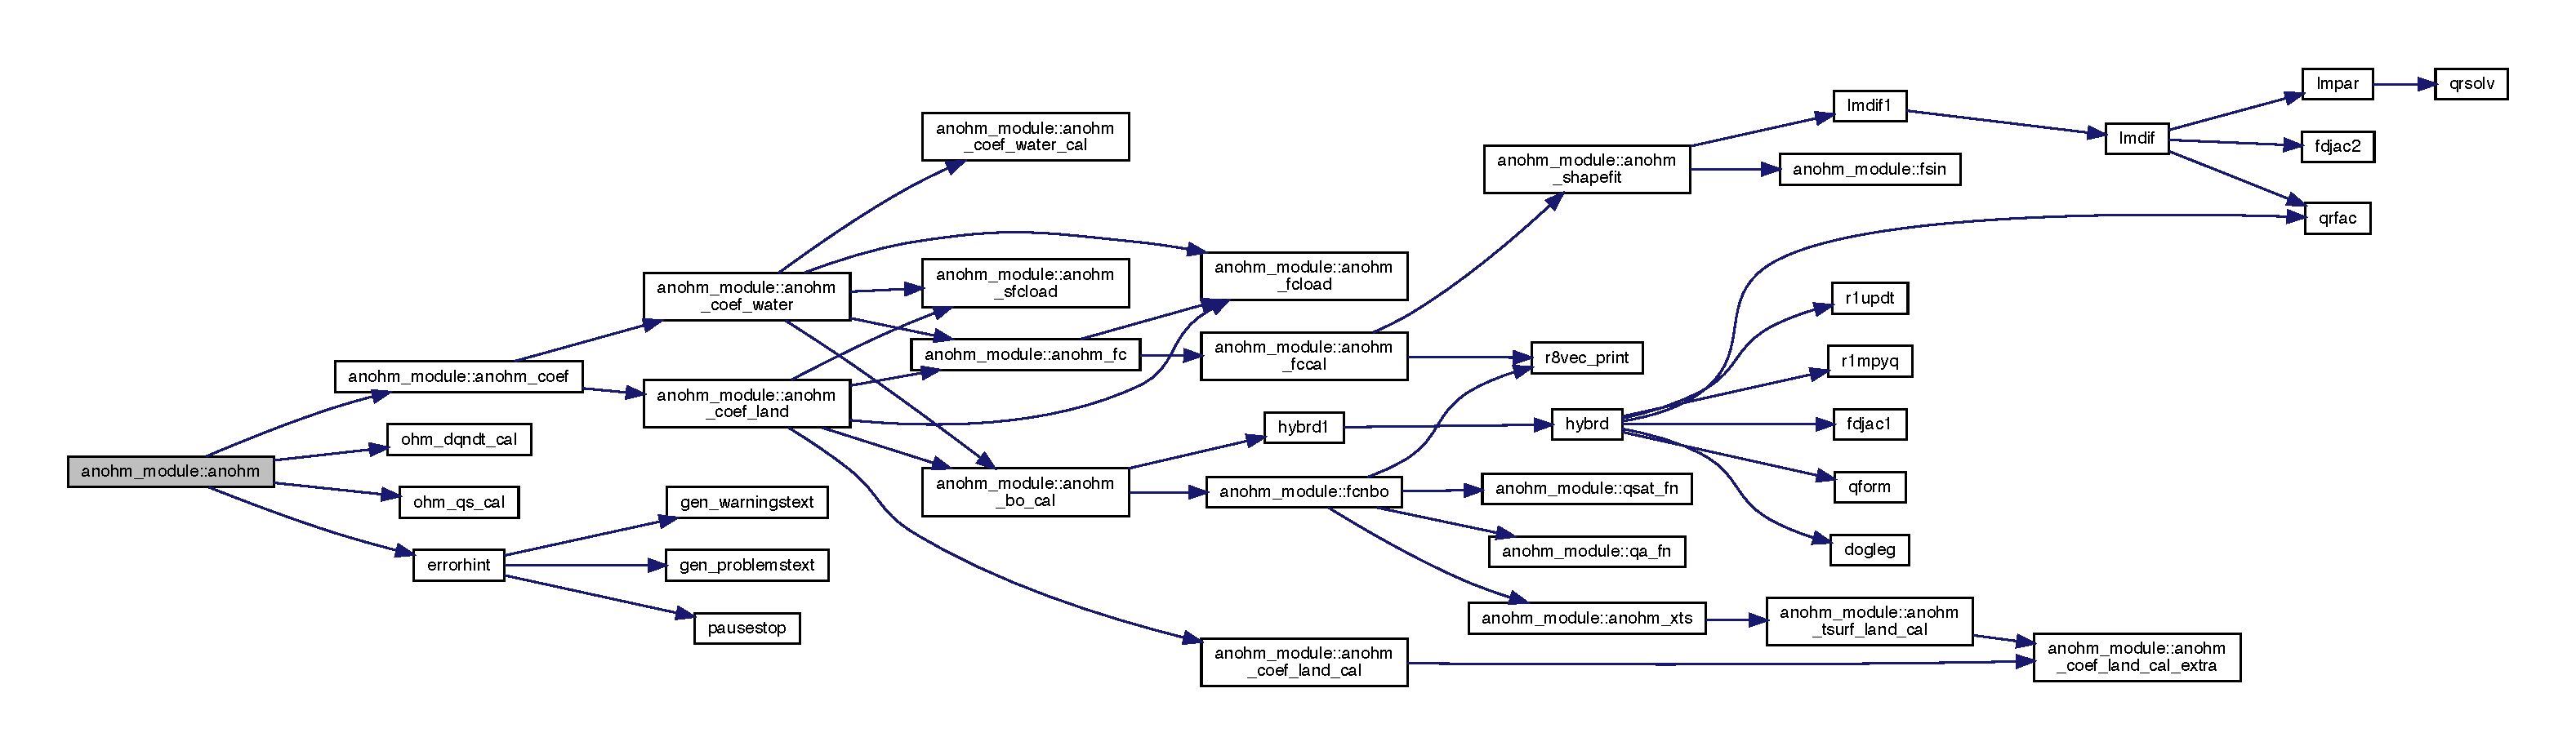
\includegraphics[width=350pt]{namespaceanohm__module_a12150b343f1a4a8c3210e499cb9db9d9_cgraph}
\end{center}
\end{figure}
\mbox{\Hypertarget{namespaceanohm__module_a7c747a2204089f0681ae47c92bf7d1e0}\label{namespaceanohm__module_a7c747a2204089f0681ae47c92bf7d1e0}} 
\index{anohm\+\_\+module@{anohm\+\_\+module}!anohm\+\_\+bo\+\_\+cal@{anohm\+\_\+bo\+\_\+cal}}
\index{anohm\+\_\+bo\+\_\+cal@{anohm\+\_\+bo\+\_\+cal}!anohm\+\_\+module@{anohm\+\_\+module}}
\subsubsection{\texorpdfstring{anohm\+\_\+bo\+\_\+cal()}{anohm\_bo\_cal()}}
{\footnotesize\ttfamily subroutine anohm\+\_\+module\+::anohm\+\_\+bo\+\_\+cal (\begin{DoxyParamCaption}\item[{real(kind = 8), dimension(\+:), intent(in)}]{Ta,  }\item[{real(kind = 8), dimension(\+:), intent(in)}]{RH,  }\item[{real(kind = 8), dimension(\+:), intent(in)}]{pres,  }\item[{real(kind = 8), dimension(\+:), intent(in)}]{t\+Hr,  }\item[{real(kind(1d0)), intent(in)}]{A\+Sd,  }\item[{real(kind(1d0)), intent(in)}]{m\+Sd,  }\item[{real(kind(1d0)), intent(in)}]{A\+Ta,  }\item[{real(kind(1d0)), intent(in)}]{m\+Ta,  }\item[{real(kind(1d0)), intent(in)}]{tau,  }\item[{real(kind(1d0)), intent(in)}]{m\+WS,  }\item[{real(kind(1d0)), intent(in)}]{m\+WF,  }\item[{real(kind(1d0)), intent(in)}]{m\+AH,  }\item[{real(kind(1d0)), intent(in)}]{xalb,  }\item[{real(kind(1d0)), intent(in)}]{xemis,  }\item[{real(kind(1d0)), intent(in)}]{xcp,  }\item[{real(kind(1d0)), intent(in)}]{xk,  }\item[{real(kind(1d0)), intent(in)}]{xch,  }\item[{real(kind(1d0)), intent(in)}]{x\+SM,  }\item[{real(kind(1d0)), intent(in)}]{t\+Sd,  }\item[{real(kind=8), intent(out)}]{x\+Bo }\end{DoxyParamCaption})}



estimate daytime Bowen ratio for calculation of An\+O\+HM coefficients 


\begin{DoxyParams}[1]{Parameters}
\mbox{\tt in}  & {\em ta} & air temperature, degC\\
\hline
\mbox{\tt in}  & {\em rh} & relative humidity, \%\\
\hline
\mbox{\tt in}  & {\em pres} & Atmospheric pressure, mbar\\
\hline
\mbox{\tt in}  & {\em thr} & time, hour\\
\hline
\mbox{\tt in}  & {\em asd} & daily amplitude of solar radiation\\
\hline
\mbox{\tt in}  & {\em msd} & daily mean solar radiation\\
\hline
\mbox{\tt in}  & {\em tsd} & local peaking time of solar radiation, hour\\
\hline
\mbox{\tt in}  & {\em ata} & daily amplitude of air temperature\\
\hline
\mbox{\tt in}  & {\em mta} & daily mean air temperature\\
\hline
\mbox{\tt in}  & {\em tau} & phase lag between Sd and Ta (Ta-\/\+Sd)\\
\hline
\mbox{\tt in}  & {\em mws} & daily mean wind speed\\
\hline
\mbox{\tt in}  & {\em mwf} & daily mean underground moisture flux\\
\hline
\mbox{\tt in}  & {\em mah} & daily mean anthropogenic heat flux\\
\hline
\mbox{\tt in}  & {\em xalb} & albedo,\\
\hline
\mbox{\tt in}  & {\em xemis} & emissivity,\\
\hline
\mbox{\tt in}  & {\em xcp} & heat capacity,\\
\hline
\mbox{\tt in}  & {\em xk} & thermal conductivity,\\
\hline
\mbox{\tt in}  & {\em xch} & bulk transfer coef.\\
\hline
\mbox{\tt in}  & {\em xsm} & surface moisture status, non-\/dimensional \\
\hline
\end{DoxyParams}


Definition at line 1375 of file S\+U\+E\+W\+S\+\_\+\+An\+O\+H\+M.\+f95.

Here is the call graph for this function\+:\nopagebreak
\begin{figure}[H]
\begin{center}
\leavevmode
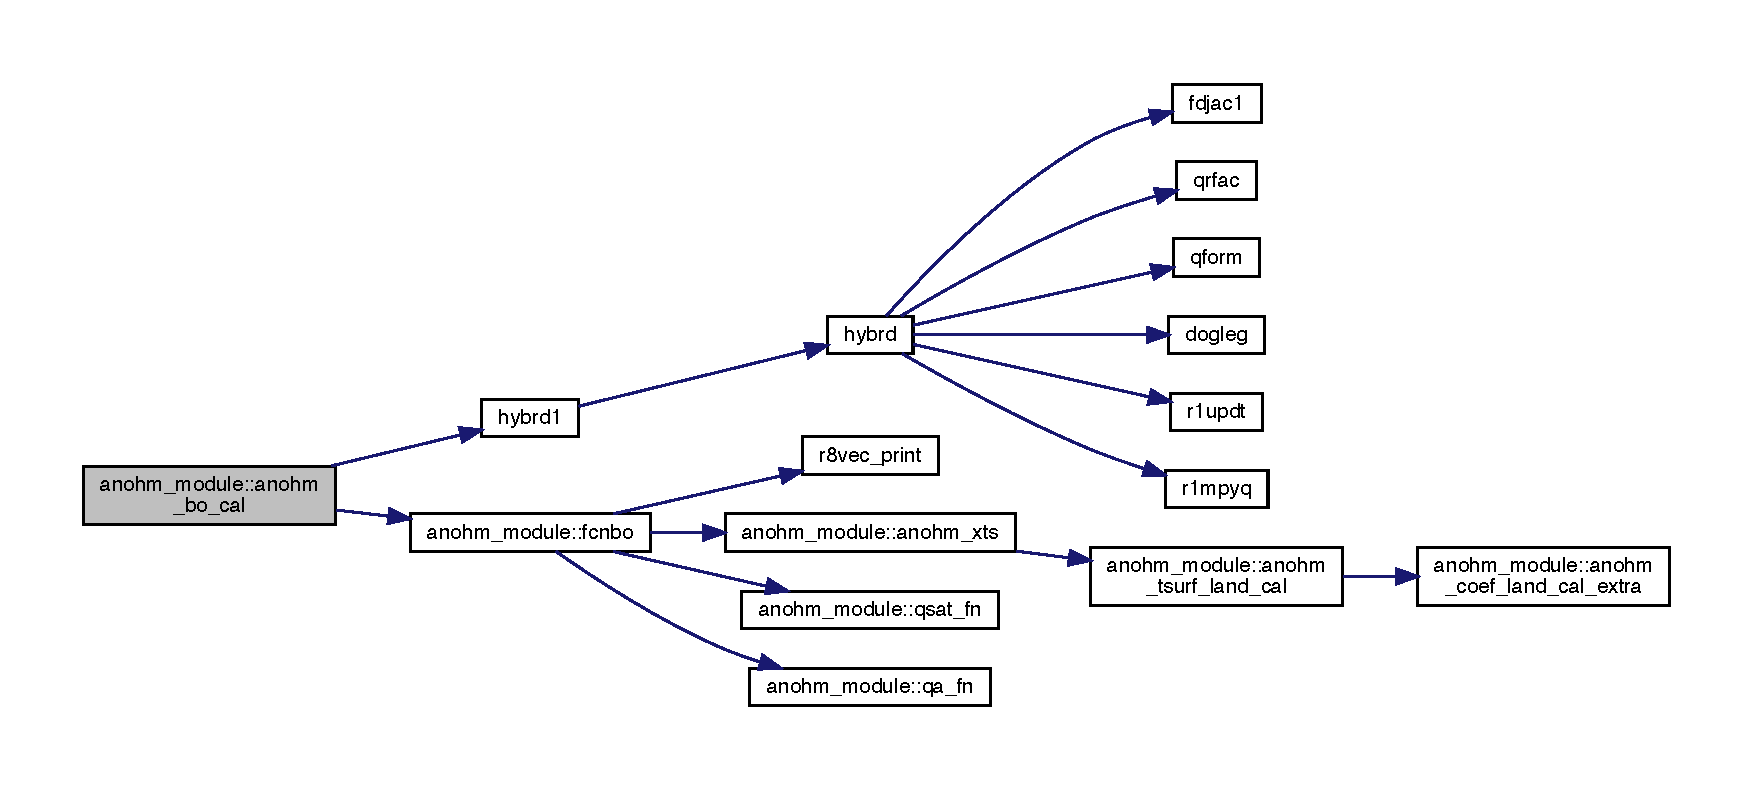
\includegraphics[width=350pt]{namespaceanohm__module_a7c747a2204089f0681ae47c92bf7d1e0_cgraph}
\end{center}
\end{figure}
\mbox{\Hypertarget{namespaceanohm__module_a5aa773c6b5c4a66155eaeb1c86c70471}\label{namespaceanohm__module_a5aa773c6b5c4a66155eaeb1c86c70471}} 
\index{anohm\+\_\+module@{anohm\+\_\+module}!anohm\+\_\+coef@{anohm\+\_\+coef}}
\index{anohm\+\_\+coef@{anohm\+\_\+coef}!anohm\+\_\+module@{anohm\+\_\+module}}
\subsubsection{\texorpdfstring{anohm\+\_\+coef()}{anohm\_coef()}}
{\footnotesize\ttfamily subroutine anohm\+\_\+module\+::anohm\+\_\+coef (\begin{DoxyParamCaption}\item[{integer, intent(in)}]{sfc\+\_\+typ,  }\item[{integer, intent(in)}]{xid,  }\item[{integer, intent(in)}]{xgrid,  }\item[{real(kind(1d0)), dimension(\+:,\+:), intent(in)}]{Met\+Forcing\+Data\+\_\+grid,  }\item[{real(kind(1d0)), dimension(\+:), intent(in)}]{moist\+\_\+surf,  }\item[{integer, intent(in)}]{Anthrop\+Heat\+Method,  }\item[{real(kind(1d0)), dimension(\+:), intent(in)}]{alb,  }\item[{real(kind(1d0)), dimension(\+:), intent(in)}]{emis,  }\item[{real(kind(1d0)), dimension(\+:), intent(in)}]{cp,  }\item[{real(kind(1d0)), dimension(\+:), intent(in)}]{kk,  }\item[{real(kind(1d0)), dimension(\+:), intent(in)}]{ch,  }\item[{real(kind(1d0)), intent(out)}]{xa1,  }\item[{real(kind(1d0)), intent(out)}]{xa2,  }\item[{real(kind(1d0)), intent(out)}]{xa3 }\end{DoxyParamCaption})}



High level wrapper for An\+O\+HM coefficients calculation. 

calculate O\+HM coefficients within An\+O\+HM framework. \begin{DoxyReturn}{Returns}

\begin{DoxyEnumerate}
\item O\+HM coefficients of a given surface type\+: a1, a2 and a3
\end{DoxyEnumerate}
\end{DoxyReturn}

\begin{DoxyParams}[1]{Parameters}
\mbox{\tt in}  & {\em moist\+\_\+surf} & surface wetness status \\
\hline
\end{DoxyParams}


Definition at line 150 of file S\+U\+E\+W\+S\+\_\+\+An\+O\+H\+M.\+f95.

Here is the call graph for this function\+:\nopagebreak
\begin{figure}[H]
\begin{center}
\leavevmode
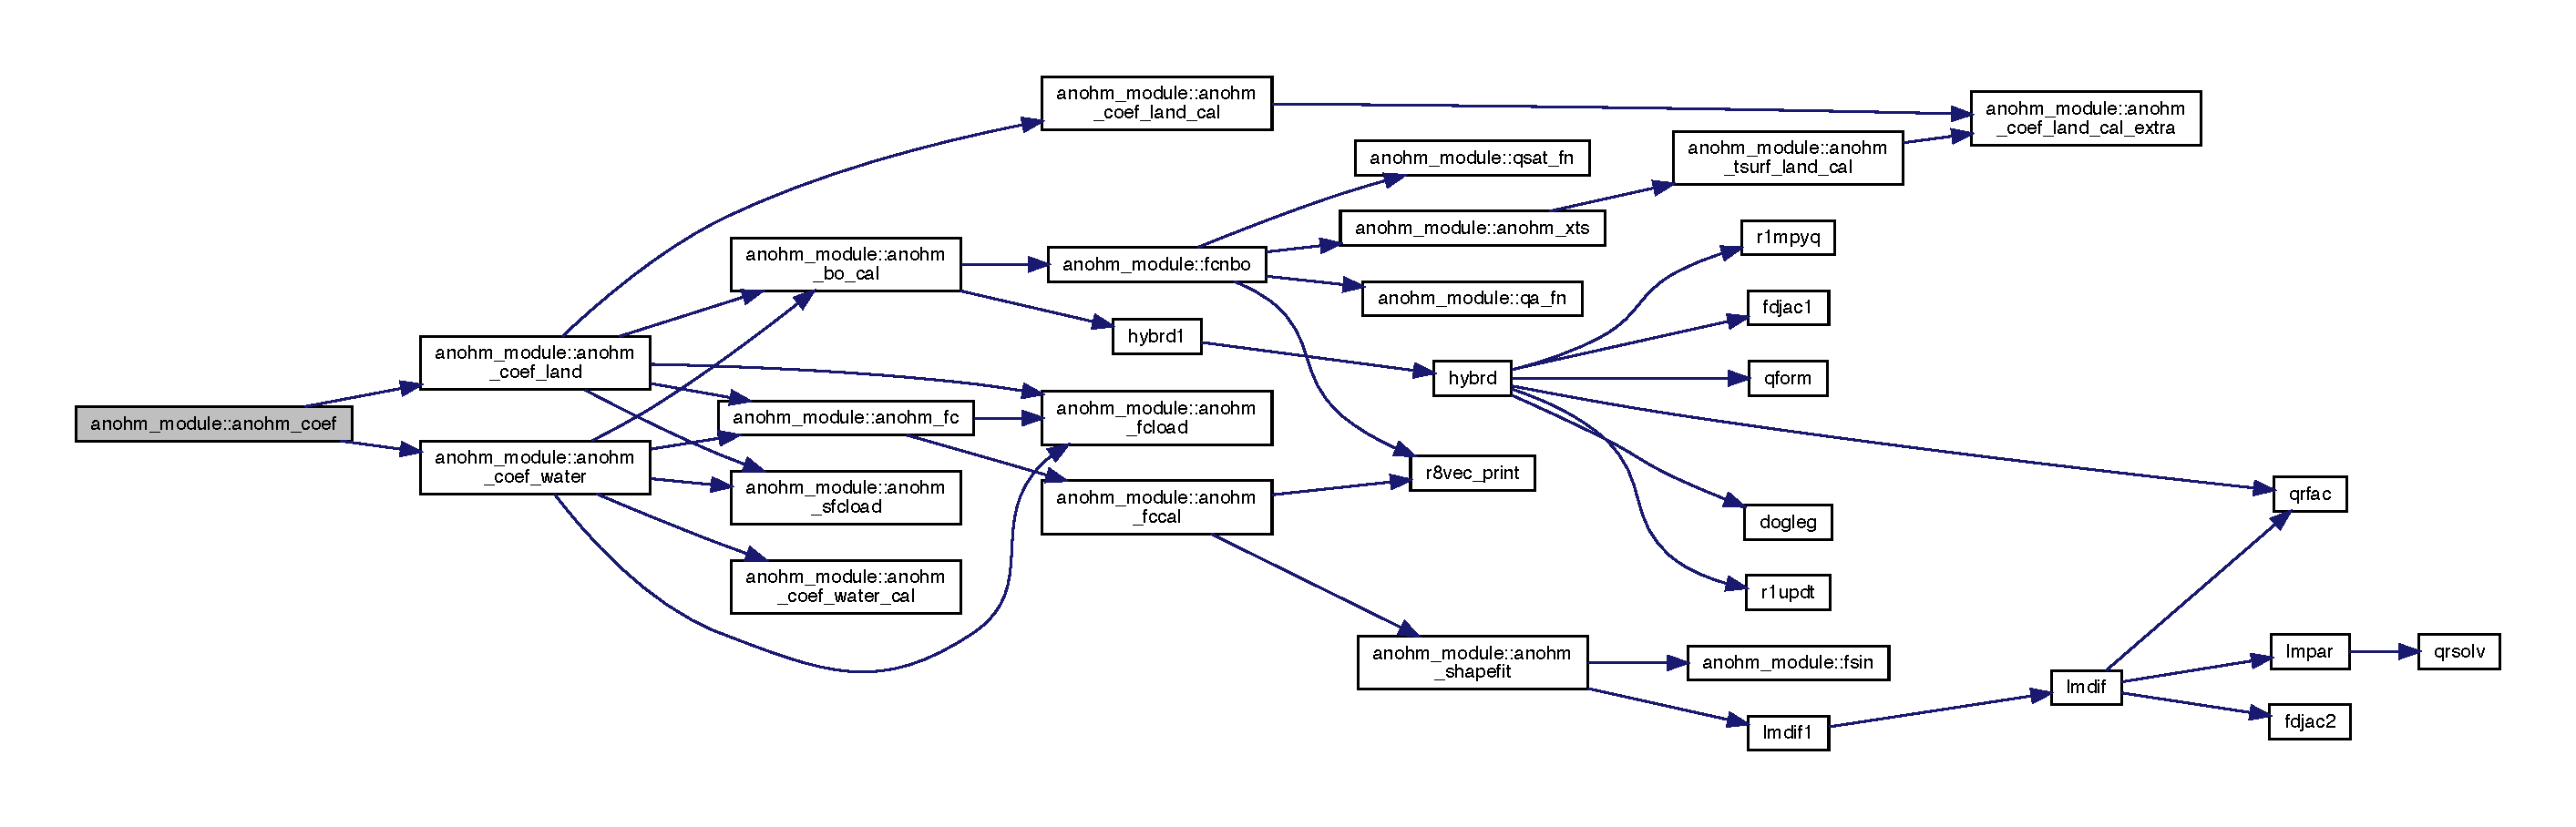
\includegraphics[width=350pt]{namespaceanohm__module_a5aa773c6b5c4a66155eaeb1c86c70471_cgraph}
\end{center}
\end{figure}
\mbox{\Hypertarget{namespaceanohm__module_abe3a233f6e7d95775554ccc25e1cac45}\label{namespaceanohm__module_abe3a233f6e7d95775554ccc25e1cac45}} 
\index{anohm\+\_\+module@{anohm\+\_\+module}!anohm\+\_\+coef\+\_\+land@{anohm\+\_\+coef\+\_\+land}}
\index{anohm\+\_\+coef\+\_\+land@{anohm\+\_\+coef\+\_\+land}!anohm\+\_\+module@{anohm\+\_\+module}}
\subsubsection{\texorpdfstring{anohm\+\_\+coef\+\_\+land()}{anohm\_coef\_land()}}
{\footnotesize\ttfamily subroutine anohm\+\_\+module\+::anohm\+\_\+coef\+\_\+land (\begin{DoxyParamCaption}\item[{integer, intent(in)}]{sfc\+\_\+typ,  }\item[{integer, intent(in)}]{xid,  }\item[{real(kind(1d0)), dimension(\+:,\+:), intent(in)}]{Met\+Forcing\+Data\+\_\+grid,  }\item[{integer, intent(in)}]{Anthrop\+Heat\+Method,  }\item[{real(kind(1d0)), dimension(\+:), intent(in)}]{moist\+\_\+surf,  }\item[{real(kind(1d0)), dimension(\+:), intent(in)}]{alb,  }\item[{real(kind(1d0)), dimension(\+:), intent(in)}]{emis,  }\item[{real(kind(1d0)), dimension(\+:), intent(in)}]{cp,  }\item[{real(kind(1d0)), dimension(\+:), intent(in)}]{kk,  }\item[{real(kind(1d0)), dimension(\+:), intent(in)}]{ch,  }\item[{real(kind(1d0)), intent(out)}]{xa1,  }\item[{real(kind(1d0)), intent(out)}]{xa2,  }\item[{real(kind(1d0)), intent(out)}]{xa3 }\end{DoxyParamCaption})}



a procedure for calculating An\+O\+HM coefficients of land surfaces 


\begin{DoxyParams}[1]{Parameters}
\mbox{\tt in}  & {\em moist\+\_\+surf} & surface wetness status \\
\hline
\end{DoxyParams}


Definition at line 218 of file S\+U\+E\+W\+S\+\_\+\+An\+O\+H\+M.\+f95.

Here is the call graph for this function\+:\nopagebreak
\begin{figure}[H]
\begin{center}
\leavevmode
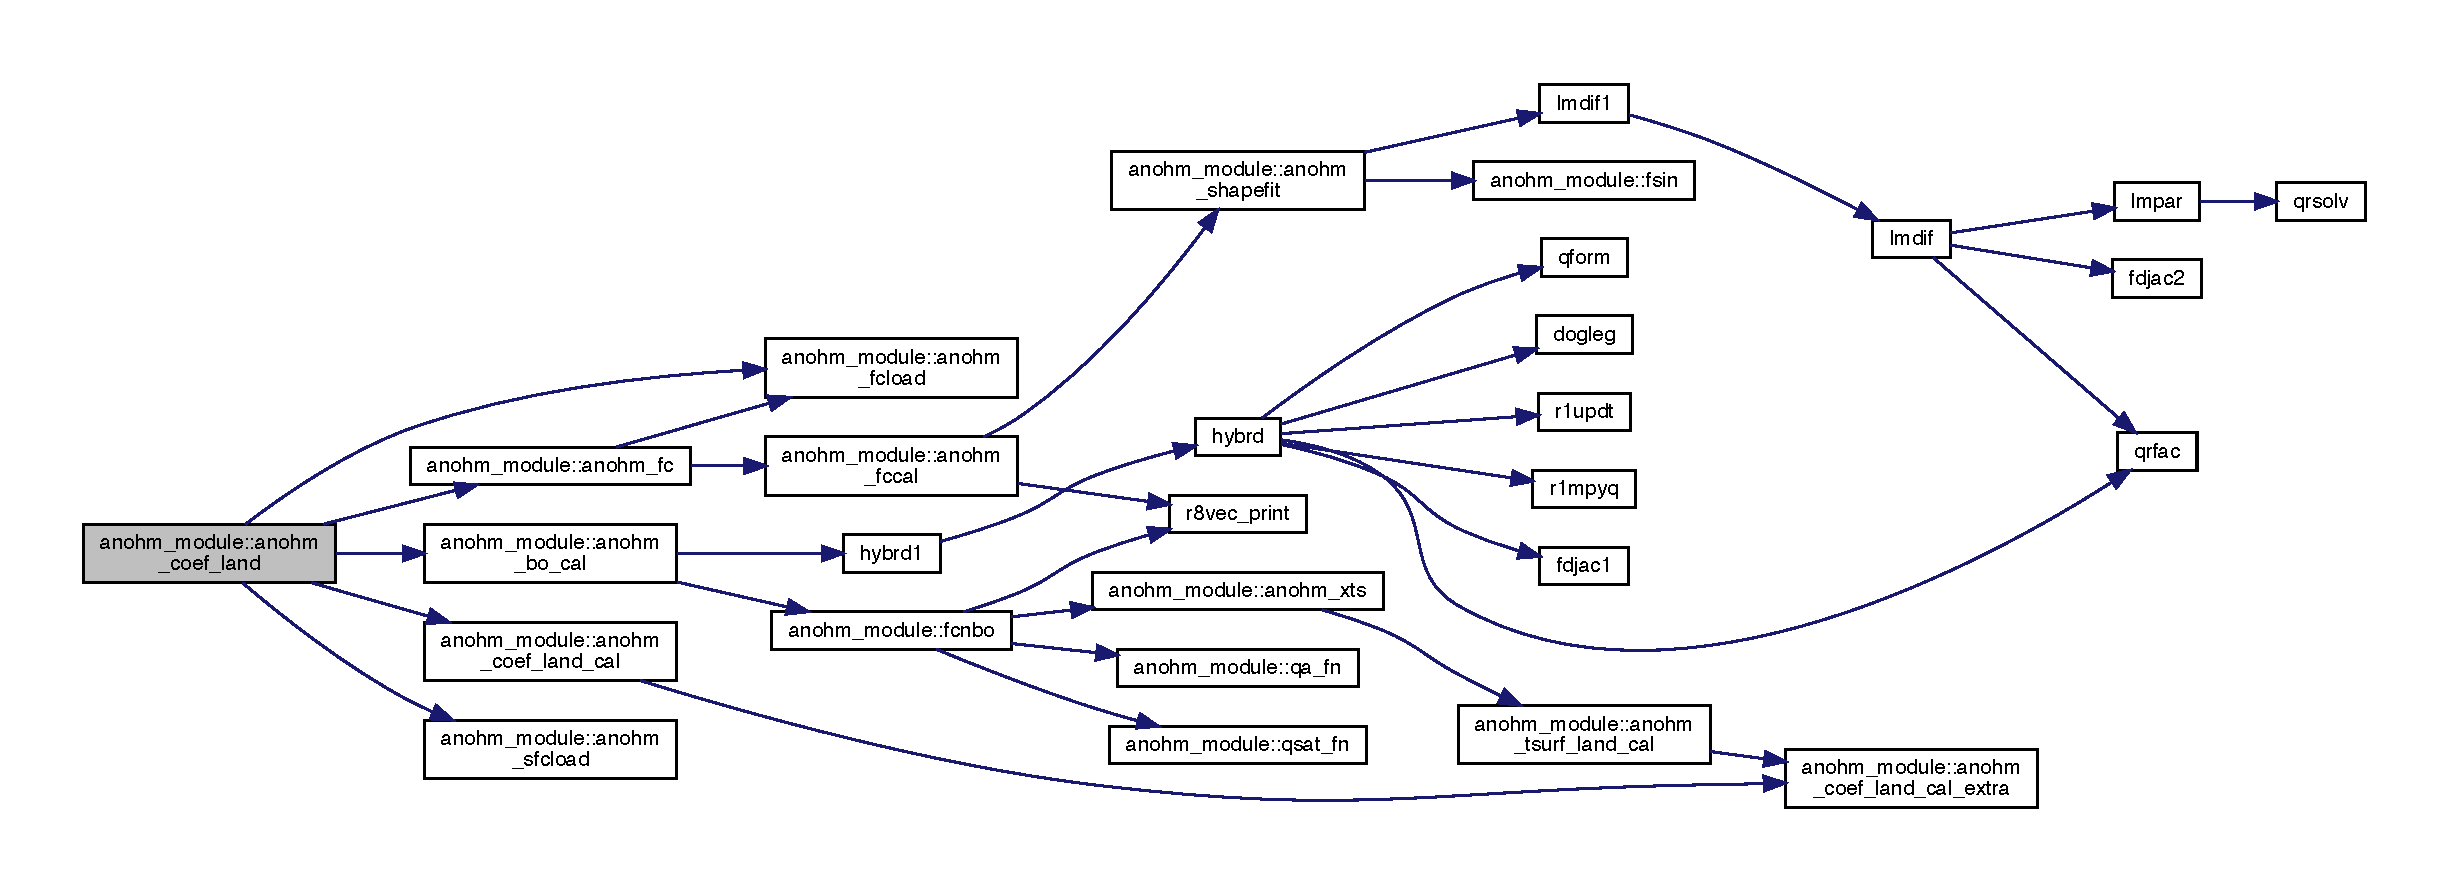
\includegraphics[width=350pt]{namespaceanohm__module_abe3a233f6e7d95775554ccc25e1cac45_cgraph}
\end{center}
\end{figure}
\mbox{\Hypertarget{namespaceanohm__module_a20235f7bc1aada21135014d0e942e59f}\label{namespaceanohm__module_a20235f7bc1aada21135014d0e942e59f}} 
\index{anohm\+\_\+module@{anohm\+\_\+module}!anohm\+\_\+coef\+\_\+land\+\_\+cal@{anohm\+\_\+coef\+\_\+land\+\_\+cal}}
\index{anohm\+\_\+coef\+\_\+land\+\_\+cal@{anohm\+\_\+coef\+\_\+land\+\_\+cal}!anohm\+\_\+module@{anohm\+\_\+module}}
\subsubsection{\texorpdfstring{anohm\+\_\+coef\+\_\+land\+\_\+cal()}{anohm\_coef\_land\_cal()}}
{\footnotesize\ttfamily subroutine anohm\+\_\+module\+::anohm\+\_\+coef\+\_\+land\+\_\+cal (\begin{DoxyParamCaption}\item[{real(kind(1d0)), intent(in)}]{A\+Sd,  }\item[{real(kind(1d0)), intent(in)}]{m\+Sd,  }\item[{real(kind(1d0)), intent(in)}]{A\+Ta,  }\item[{real(kind(1d0)), intent(in)}]{m\+Ta,  }\item[{real(kind(1d0)), intent(in)}]{tau,  }\item[{real(kind(1d0)), intent(in)}]{m\+WS,  }\item[{real(kind(1d0)), intent(in)}]{m\+WF,  }\item[{real(kind(1d0)), intent(in)}]{m\+AH,  }\item[{real(kind(1d0)), intent(in)}]{xalb,  }\item[{real(kind(1d0)), intent(in)}]{xemis,  }\item[{real(kind(1d0)), intent(in)}]{xcp,  }\item[{real(kind(1d0)), intent(in)}]{xk,  }\item[{real(kind(1d0)), intent(in)}]{xch,  }\item[{real(kind(1d0)), intent(in)}]{x\+Bo,  }\item[{real(kind(1d0)), intent(out)}]{xa1,  }\item[{real(kind(1d0)), intent(out)}]{xa2,  }\item[{real(kind(1d0)), intent(out)}]{xa3 }\end{DoxyParamCaption})}



a wrapper for retrieving An\+O\+HM coefficients 

\begin{DoxyReturn}{Returns}

\begin{DoxyEnumerate}
\item O\+HM coefficients of a given surface type\+: a1, a2 and a3
\end{DoxyEnumerate}
\end{DoxyReturn}

\begin{DoxyParams}[1]{Parameters}
\mbox{\tt in}  & {\em asd} & daily amplitude of solar radiation\\
\hline
\mbox{\tt in}  & {\em msd} & daily mean solar radiation\\
\hline
\mbox{\tt in}  & {\em ata} & daily amplitude of air temperature\\
\hline
\mbox{\tt in}  & {\em mta} & daily mean air temperature\\
\hline
\mbox{\tt in}  & {\em tau} & phase lag between Sd and Ta (Ta-\/\+Sd)\\
\hline
\mbox{\tt in}  & {\em mws} & daily mean wind speed\\
\hline
\mbox{\tt in}  & {\em mwf} & daily mean underground moisture flux\\
\hline
\mbox{\tt in}  & {\em mah} & daily mean anthropogenic heat flux\\
\hline
\mbox{\tt in}  & {\em xalb} & albedo\\
\hline
\mbox{\tt in}  & {\em xemis} & emissivity\\
\hline
\mbox{\tt in}  & {\em xcp} & heat capacity\\
\hline
\mbox{\tt in}  & {\em xk} & thermal conductivity\\
\hline
\mbox{\tt in}  & {\em xch} & bulk transfer coef\\
\hline
\mbox{\tt in}  & {\em xbo} & Bowen ratio\\
\hline
\mbox{\tt out}  & {\em xa1} & a1\\
\hline
\mbox{\tt out}  & {\em xa2} & a2\\
\hline
\mbox{\tt out}  & {\em xa3} & a3 \\
\hline
\end{DoxyParams}


Definition at line 312 of file S\+U\+E\+W\+S\+\_\+\+An\+O\+H\+M.\+f95.

Here is the call graph for this function\+:\nopagebreak
\begin{figure}[H]
\begin{center}
\leavevmode
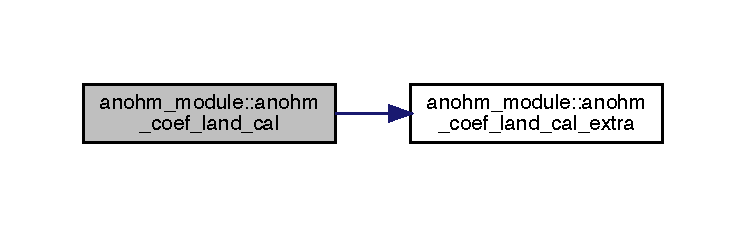
\includegraphics[width=350pt]{namespaceanohm__module_a20235f7bc1aada21135014d0e942e59f_cgraph}
\end{center}
\end{figure}
\mbox{\Hypertarget{namespaceanohm__module_ab96821e3f733aae01d895aa8830085b7}\label{namespaceanohm__module_ab96821e3f733aae01d895aa8830085b7}} 
\index{anohm\+\_\+module@{anohm\+\_\+module}!anohm\+\_\+coef\+\_\+land\+\_\+cal\+\_\+extra@{anohm\+\_\+coef\+\_\+land\+\_\+cal\+\_\+extra}}
\index{anohm\+\_\+coef\+\_\+land\+\_\+cal\+\_\+extra@{anohm\+\_\+coef\+\_\+land\+\_\+cal\+\_\+extra}!anohm\+\_\+module@{anohm\+\_\+module}}
\subsubsection{\texorpdfstring{anohm\+\_\+coef\+\_\+land\+\_\+cal\+\_\+extra()}{anohm\_coef\_land\_cal\_extra()}}
{\footnotesize\ttfamily subroutine anohm\+\_\+module\+::anohm\+\_\+coef\+\_\+land\+\_\+cal\+\_\+extra (\begin{DoxyParamCaption}\item[{real(kind(1d0)), intent(in)}]{A\+Sd,  }\item[{real(kind(1d0)), intent(in)}]{m\+Sd,  }\item[{real(kind(1d0)), intent(in)}]{A\+Ta,  }\item[{real(kind(1d0)), intent(in)}]{m\+Ta,  }\item[{real(kind(1d0)), intent(in)}]{tau,  }\item[{real(kind(1d0)), intent(in)}]{m\+WS,  }\item[{real(kind(1d0)), intent(in)}]{m\+WF,  }\item[{real(kind(1d0)), intent(in)}]{m\+AH,  }\item[{real(kind(1d0)), intent(in)}]{xalb,  }\item[{real(kind(1d0)), intent(in)}]{xemis,  }\item[{real(kind(1d0)), intent(in)}]{xcp,  }\item[{real(kind(1d0)), intent(in)}]{xk,  }\item[{real(kind(1d0)), intent(in)}]{xch,  }\item[{real(kind(1d0)), intent(in)}]{x\+Bo,  }\item[{real(kind(1d0)), intent(out)}]{xa1,  }\item[{real(kind(1d0)), intent(out)}]{xa2,  }\item[{real(kind(1d0)), intent(out)}]{xa3,  }\item[{real(kind(1d0)), intent(out)}]{A\+Ts,  }\item[{real(kind(1d0)), intent(out)}]{m\+Ts,  }\item[{real(kind(1d0)), intent(out)}]{gamma }\end{DoxyParamCaption})}


\begin{DoxyParams}[1]{Parameters}
\mbox{\tt in}  & {\em asd} & daily amplitude of solar radiation\\
\hline
\mbox{\tt in}  & {\em msd} & daily mean solar radiation\\
\hline
\mbox{\tt in}  & {\em ata} & daily amplitude of air temperature\\
\hline
\mbox{\tt in}  & {\em mta} & daily mean air temperature\\
\hline
\mbox{\tt in}  & {\em tau} & phase lag between Sd and Ta (Ta-\/\+Sd)\\
\hline
\mbox{\tt in}  & {\em mws} & daily mean wind speed\\
\hline
\mbox{\tt in}  & {\em mwf} & daily mean underground moisture flux\\
\hline
\mbox{\tt in}  & {\em mah} & daily mean anthropogenic heat flux\\
\hline
\mbox{\tt in}  & {\em xalb} & albedo\\
\hline
\mbox{\tt in}  & {\em xemis} & emissivity\\
\hline
\mbox{\tt in}  & {\em xcp} & heat capacity\\
\hline
\mbox{\tt in}  & {\em xk} & thermal conductivity\\
\hline
\mbox{\tt in}  & {\em xch} & bulk transfer coef\\
\hline
\mbox{\tt in}  & {\em xbo} & Bowen ratio\\
\hline
\mbox{\tt out}  & {\em xa1} & a1\\
\hline
\mbox{\tt out}  & {\em xa2} & a2\\
\hline
\mbox{\tt out}  & {\em xa3} & a3\\
\hline
\mbox{\tt out}  & {\em ats} & daily amplitude of surface temperature\\
\hline
\mbox{\tt out}  & {\em mts} & daily mean of surface temperature\\
\hline
\mbox{\tt out}  & {\em gamma} & phase difference between Ts and Sd \\
\hline
\end{DoxyParams}


Definition at line 464 of file S\+U\+E\+W\+S\+\_\+\+An\+O\+H\+M.\+f95.

\mbox{\Hypertarget{namespaceanohm__module_a5b0b99ebb9db9ec50d904cc7a9802779}\label{namespaceanohm__module_a5b0b99ebb9db9ec50d904cc7a9802779}} 
\index{anohm\+\_\+module@{anohm\+\_\+module}!anohm\+\_\+coef\+\_\+water@{anohm\+\_\+coef\+\_\+water}}
\index{anohm\+\_\+coef\+\_\+water@{anohm\+\_\+coef\+\_\+water}!anohm\+\_\+module@{anohm\+\_\+module}}
\subsubsection{\texorpdfstring{anohm\+\_\+coef\+\_\+water()}{anohm\_coef\_water()}}
{\footnotesize\ttfamily subroutine anohm\+\_\+module\+::anohm\+\_\+coef\+\_\+water (\begin{DoxyParamCaption}\item[{integer, intent(in)}]{sfc\+\_\+typ,  }\item[{integer, intent(in)}]{xid,  }\item[{real(kind(1d0)), dimension(\+:,\+:), intent(in)}]{Met\+Forcing\+Data\+\_\+grid,  }\item[{integer, intent(in)}]{Anthrop\+Heat\+Method,  }\item[{real(kind(1d0)), dimension(\+:), intent(in)}]{moist\+\_\+surf,  }\item[{real(kind(1d0)), dimension(\+:), intent(in)}]{alb,  }\item[{real(kind(1d0)), dimension(\+:), intent(in)}]{emis,  }\item[{real(kind(1d0)), dimension(\+:), intent(in)}]{cp,  }\item[{real(kind(1d0)), dimension(\+:), intent(in)}]{kk,  }\item[{real(kind(1d0)), dimension(\+:), intent(in)}]{ch,  }\item[{real(kind(1d0)), intent(out)}]{xa1,  }\item[{real(kind(1d0)), intent(out)}]{xa2,  }\item[{real(kind(1d0)), intent(out)}]{xa3 }\end{DoxyParamCaption})}



a procedure for calculating An\+O\+HM coefficients of water body based on forcings and sfc. conditions 

\+: NB\+: this S\+U\+B\+R\+O\+U\+T\+I\+NE hasn\textquotesingle{}t been well tested.


\begin{DoxyParams}[1]{Parameters}
\mbox{\tt in}  & {\em moist\+\_\+surf} & surface wetness status \\
\hline
\end{DoxyParams}


Definition at line 638 of file S\+U\+E\+W\+S\+\_\+\+An\+O\+H\+M.\+f95.

Here is the call graph for this function\+:\nopagebreak
\begin{figure}[H]
\begin{center}
\leavevmode
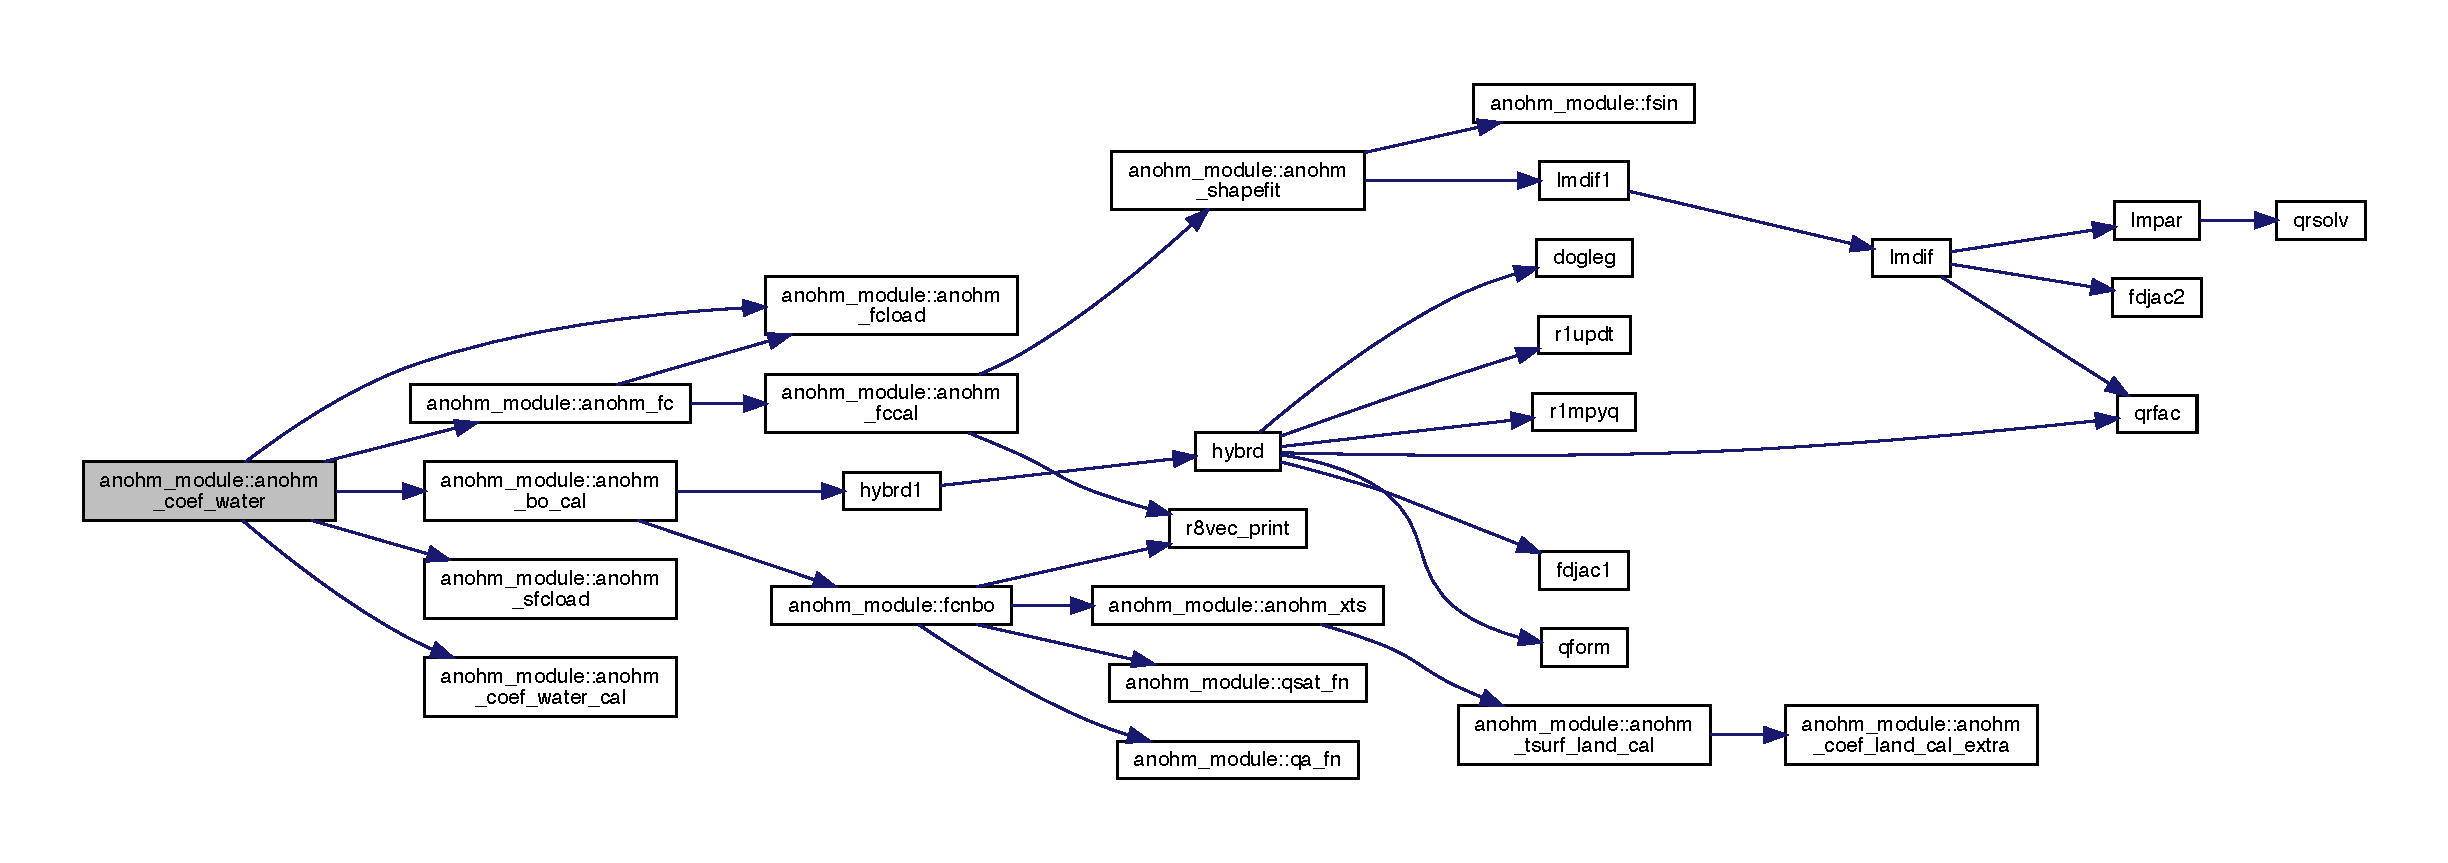
\includegraphics[width=350pt]{namespaceanohm__module_a5b0b99ebb9db9ec50d904cc7a9802779_cgraph}
\end{center}
\end{figure}
\mbox{\Hypertarget{namespaceanohm__module_aeb16132909e9aae5549d9ce6adcf389f}\label{namespaceanohm__module_aeb16132909e9aae5549d9ce6adcf389f}} 
\index{anohm\+\_\+module@{anohm\+\_\+module}!anohm\+\_\+coef\+\_\+water\+\_\+cal@{anohm\+\_\+coef\+\_\+water\+\_\+cal}}
\index{anohm\+\_\+coef\+\_\+water\+\_\+cal@{anohm\+\_\+coef\+\_\+water\+\_\+cal}!anohm\+\_\+module@{anohm\+\_\+module}}
\subsubsection{\texorpdfstring{anohm\+\_\+coef\+\_\+water\+\_\+cal()}{anohm\_coef\_water\_cal()}}
{\footnotesize\ttfamily subroutine anohm\+\_\+module\+::anohm\+\_\+coef\+\_\+water\+\_\+cal (\begin{DoxyParamCaption}\item[{real(kind(1d0)), intent(in)}]{A\+Sd,  }\item[{real(kind(1d0)), intent(in)}]{m\+Sd,  }\item[{real(kind(1d0)), intent(in)}]{A\+Ta,  }\item[{real(kind(1d0)), intent(in)}]{m\+Ta,  }\item[{real(kind(1d0)), intent(in)}]{tau,  }\item[{real(kind(1d0)), intent(in)}]{m\+WS,  }\item[{real(kind(1d0)), intent(in)}]{m\+WF,  }\item[{real(kind(1d0)), intent(in)}]{m\+AH,  }\item[{real(kind(1d0)), intent(in)}]{xalb,  }\item[{real(kind(1d0)), intent(in)}]{xemis,  }\item[{real(kind(1d0)), intent(in)}]{xcp,  }\item[{real(kind(1d0)), intent(in)}]{xk,  }\item[{real(kind(1d0)), intent(in)}]{xch,  }\item[{real(kind(1d0)), intent(in)}]{x\+Bo,  }\item[{real(kind(1d0)), intent(in)}]{xeta,  }\item[{real(kind(1d0)), intent(in)}]{xmu,  }\item[{real(kind(1d0)), intent(out)}]{xa1,  }\item[{real(kind(1d0)), intent(out)}]{xa2,  }\item[{real(kind(1d0)), intent(out)}]{xa3 }\end{DoxyParamCaption})}



a wrapper for retrieving An\+O\+HM coefficients of water body 

\begin{DoxyReturn}{Returns}

\begin{DoxyEnumerate}
\item O\+HM coefficients of a given surface type\+: a1, a2 and a3 \+: NB\+: this S\+U\+B\+R\+O\+U\+T\+I\+NE hasn\textquotesingle{}t been well tested.
\end{DoxyEnumerate}
\end{DoxyReturn}

\begin{DoxyParams}[1]{Parameters}
\mbox{\tt in}  & {\em asd} & daily amplitude of solar radiation\\
\hline
\mbox{\tt in}  & {\em msd} & daily mean solar radiation\\
\hline
\mbox{\tt in}  & {\em ata} & daily amplitude of air temperature\\
\hline
\mbox{\tt in}  & {\em mta} & daily mean air temperature\\
\hline
\mbox{\tt in}  & {\em tau} & phase lag between Sd and Ta (Ta-\/\+Sd)\\
\hline
\mbox{\tt in}  & {\em mws} & daily mean wind speed\\
\hline
\mbox{\tt in}  & {\em mwf} & daily mean underground moisture flux\\
\hline
\mbox{\tt in}  & {\em mah} & daily mean anthropogenic heat flux\\
\hline
\mbox{\tt in}  & {\em xalb} & albedo\\
\hline
\mbox{\tt in}  & {\em xemis} & emissivity\\
\hline
\mbox{\tt in}  & {\em xcp} & heat capacity\\
\hline
\mbox{\tt in}  & {\em xk} & thermal conductivity\\
\hline
\mbox{\tt in}  & {\em xch} & bulk transfer coef\\
\hline
\mbox{\tt in}  & {\em xbo} & Bowen ratio\\
\hline
\mbox{\tt in}  & {\em xeta} & effective absorption coefficient\\
\hline
\mbox{\tt in}  & {\em xmu} & effective absorption fraction\\
\hline
\mbox{\tt out}  & {\em xa1} & a1\\
\hline
\mbox{\tt out}  & {\em xa2} & a2\\
\hline
\mbox{\tt out}  & {\em xa3} & a3 \\
\hline
\end{DoxyParams}


Definition at line 735 of file S\+U\+E\+W\+S\+\_\+\+An\+O\+H\+M.\+f95.

\mbox{\Hypertarget{namespaceanohm__module_aeb3eededd40f7c2bb12213c747c93513}\label{namespaceanohm__module_aeb3eededd40f7c2bb12213c747c93513}} 
\index{anohm\+\_\+module@{anohm\+\_\+module}!anohm\+\_\+fc@{anohm\+\_\+fc}}
\index{anohm\+\_\+fc@{anohm\+\_\+fc}!anohm\+\_\+module@{anohm\+\_\+module}}
\subsubsection{\texorpdfstring{anohm\+\_\+fc()}{anohm\_fc()}}
{\footnotesize\ttfamily subroutine anohm\+\_\+module\+::anohm\+\_\+fc (\begin{DoxyParamCaption}\item[{integer, intent(in)}]{xid,  }\item[{real(kind(1d0)), dimension(\+:,\+:), intent(in)}]{Met\+Forcing\+Data\+\_\+grid,  }\item[{integer, intent(in)}]{Anthrop\+Heat\+Method,  }\item[{real(kind(1d0)), intent(out)}]{A\+Sd,  }\item[{real(kind(1d0)), intent(out)}]{m\+Sd,  }\item[{real(kind(1d0)), intent(out)}]{t\+Sd,  }\item[{real(kind(1d0)), intent(out)}]{A\+Ta,  }\item[{real(kind(1d0)), intent(out)}]{m\+Ta,  }\item[{real(kind(1d0)), intent(out)}]{t\+Ta,  }\item[{real(kind(1d0)), intent(out)}]{tau,  }\item[{real(kind(1d0)), intent(out)}]{m\+WS,  }\item[{real(kind(1d0)), intent(out)}]{m\+WF,  }\item[{real(kind(1d0)), intent(out)}]{m\+AH }\end{DoxyParamCaption})}


\begin{DoxyParams}[1]{Parameters}
\mbox{\tt out}  & {\em asd} & daily amplitude of solar radiation\\
\hline
\mbox{\tt out}  & {\em msd} & daily mean solar radiation\\
\hline
\mbox{\tt out}  & {\em tsd} & local peaking time of solar radiation, hour\\
\hline
\mbox{\tt out}  & {\em ata} & daily amplitude of air temperature\\
\hline
\mbox{\tt out}  & {\em mta} & daily mean air temperature\\
\hline
\mbox{\tt out}  & {\em tta} & local peaking time of air temperature, hour\\
\hline
\mbox{\tt out}  & {\em tau} & phase lag between Sd and Ta (Ta-\/\+Sd)\\
\hline
\mbox{\tt out}  & {\em mws} & daily mean wind speed\\
\hline
\mbox{\tt out}  & {\em mwf} & daily mean underground moisture flux\\
\hline
\mbox{\tt out}  & {\em mah} & daily mean anthropogenic heat flux \\
\hline
\end{DoxyParams}


Definition at line 900 of file S\+U\+E\+W\+S\+\_\+\+An\+O\+H\+M.\+f95.

Here is the call graph for this function\+:\nopagebreak
\begin{figure}[H]
\begin{center}
\leavevmode
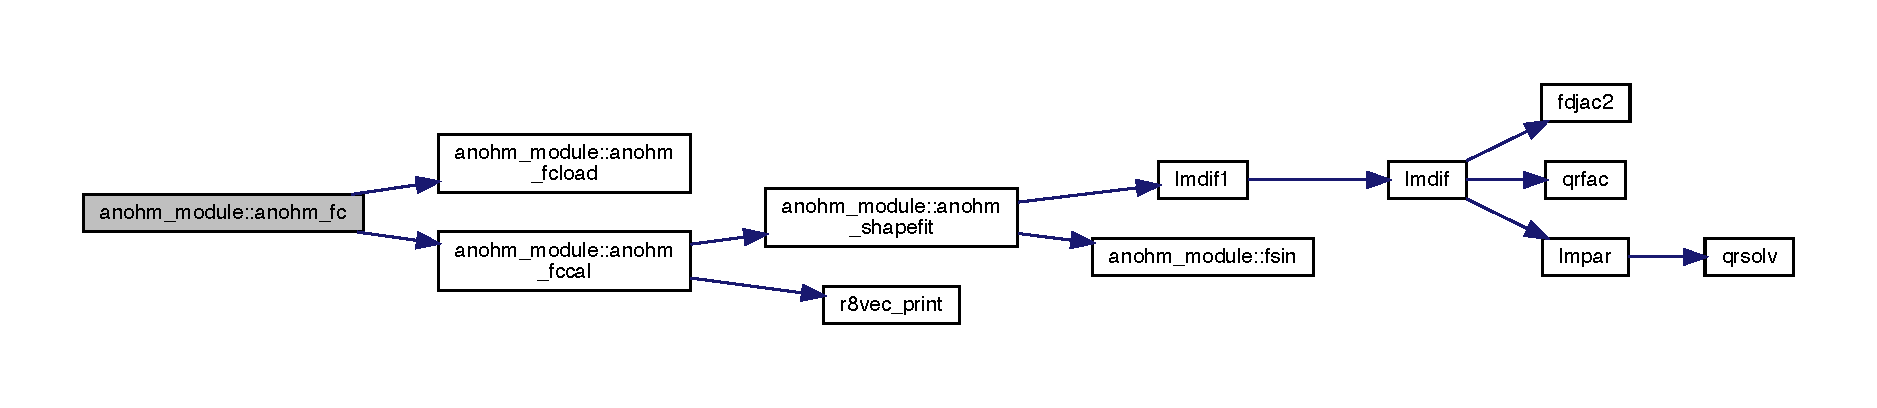
\includegraphics[width=350pt]{namespaceanohm__module_aeb3eededd40f7c2bb12213c747c93513_cgraph}
\end{center}
\end{figure}
\mbox{\Hypertarget{namespaceanohm__module_afed396f8cec94d18f3c6bec4a2a879eb}\label{namespaceanohm__module_afed396f8cec94d18f3c6bec4a2a879eb}} 
\index{anohm\+\_\+module@{anohm\+\_\+module}!anohm\+\_\+fccal@{anohm\+\_\+fccal}}
\index{anohm\+\_\+fccal@{anohm\+\_\+fccal}!anohm\+\_\+module@{anohm\+\_\+module}}
\subsubsection{\texorpdfstring{anohm\+\_\+fccal()}{anohm\_fccal()}}
{\footnotesize\ttfamily subroutine anohm\+\_\+module\+::anohm\+\_\+fccal (\begin{DoxyParamCaption}\item[{real(kind(1d0)), dimension(\+:), intent(in)}]{Sd,  }\item[{real(kind(1d0)), dimension(\+:), intent(in)}]{Ta,  }\item[{real(kind(1d0)), dimension(\+:), intent(in)}]{WS,  }\item[{real(kind(1d0)), dimension(\+:), intent(in)}]{WF,  }\item[{real(kind(1d0)), dimension(\+:), intent(in)}]{AH,  }\item[{real(kind(1d0)), dimension(\+:), intent(in)}]{t\+Hr,  }\item[{real(kind(1d0)), intent(out)}]{A\+Sd,  }\item[{real(kind(1d0)), intent(out)}]{m\+Sd,  }\item[{real(kind(1d0)), intent(out)}]{t\+Sd,  }\item[{real(kind(1d0)), intent(out)}]{A\+Ta,  }\item[{real(kind(1d0)), intent(out)}]{m\+Ta,  }\item[{real(kind(1d0)), intent(out)}]{t\+Ta,  }\item[{real(kind(1d0)), intent(out)}]{tau,  }\item[{real(kind(1d0)), intent(out)}]{m\+WS,  }\item[{real(kind(1d0)), intent(out)}]{m\+WF,  }\item[{real(kind(1d0)), intent(out)}]{m\+AH }\end{DoxyParamCaption})}



calculate the key parameters of a sinusoidal curve for An\+O\+HM forcings i.\+e., a, b, c in a$\ast$\+Sin(Pi/12$\ast$t+b)+c 


\begin{DoxyParams}[1]{Parameters}
\mbox{\tt in}  & {\em sd} & incoming shortwave radiation, W m-\/2\\
\hline
\mbox{\tt in}  & {\em ta} & air temperature, K\\
\hline
\mbox{\tt in}  & {\em ws} & wind speed, m s-\/1\\
\hline
\mbox{\tt in}  & {\em wf} & water flux density, ???\\
\hline
\mbox{\tt in}  & {\em ah} & anthropogenic heat, W m-\/2\\
\hline
\mbox{\tt in}  & {\em thr} & time in hour, hr\\
\hline
\mbox{\tt out}  & {\em asd} & daily amplitude of solar radiation\\
\hline
\mbox{\tt out}  & {\em msd} & daily mean solar radiation\\
\hline
\mbox{\tt out}  & {\em tsd} & local peaking time of solar radiation, hour\\
\hline
\mbox{\tt out}  & {\em ata} & daily amplitude of air temperature\\
\hline
\mbox{\tt out}  & {\em mta} & daily mean air temperature\\
\hline
\mbox{\tt out}  & {\em tta} & local peaking time of air temperature, hour\\
\hline
\mbox{\tt out}  & {\em tau} & phase lag between Sd and Ta (Ta-\/\+Sd)\\
\hline
\mbox{\tt out}  & {\em mws} & daily mean wind speed\\
\hline
\mbox{\tt out}  & {\em mwf} & daily mean underground moisture flux\\
\hline
\mbox{\tt out}  & {\em mah} & daily mean anthropogenic heat flux \\
\hline
\end{DoxyParams}


Definition at line 1058 of file S\+U\+E\+W\+S\+\_\+\+An\+O\+H\+M.\+f95.

Here is the call graph for this function\+:\nopagebreak
\begin{figure}[H]
\begin{center}
\leavevmode
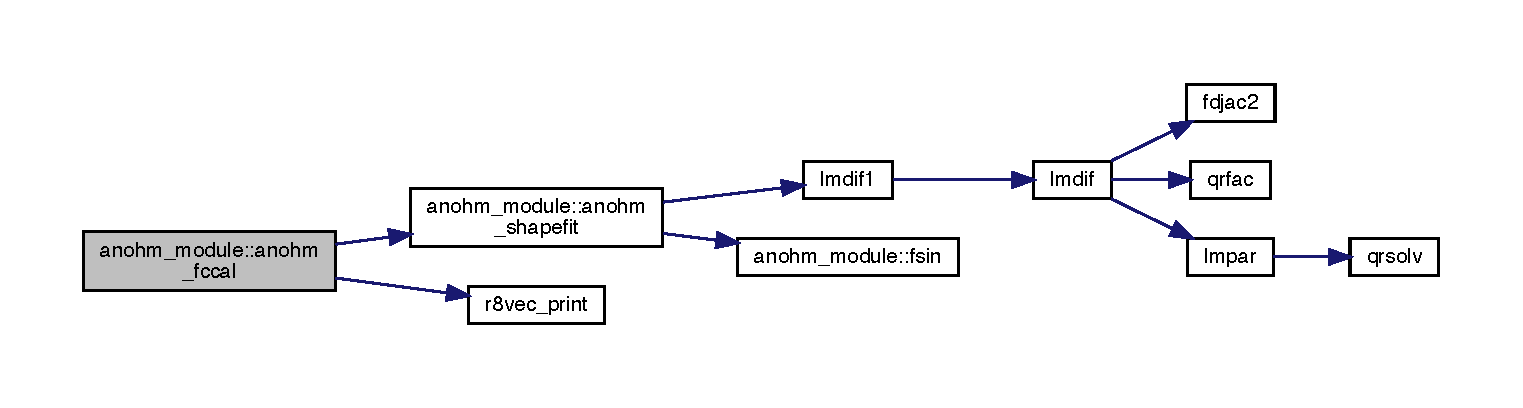
\includegraphics[width=350pt]{namespaceanohm__module_afed396f8cec94d18f3c6bec4a2a879eb_cgraph}
\end{center}
\end{figure}
\mbox{\Hypertarget{namespaceanohm__module_ae189523211fd4b943a0e75cbc1e7b7d1}\label{namespaceanohm__module_ae189523211fd4b943a0e75cbc1e7b7d1}} 
\index{anohm\+\_\+module@{anohm\+\_\+module}!anohm\+\_\+fcload@{anohm\+\_\+fcload}}
\index{anohm\+\_\+fcload@{anohm\+\_\+fcload}!anohm\+\_\+module@{anohm\+\_\+module}}
\subsubsection{\texorpdfstring{anohm\+\_\+fcload()}{anohm\_fcload()}}
{\footnotesize\ttfamily subroutine anohm\+\_\+module\+::anohm\+\_\+fcload (\begin{DoxyParamCaption}\item[{integer, intent(in)}]{xid,  }\item[{real(kind(1d0)), dimension(\+:,\+:), intent(in)}]{Met\+Forcing\+Data\+\_\+grid,  }\item[{integer, intent(in)}]{Anthrop\+Heat\+Method,  }\item[{real(kind(1d0)), dimension(\+:), intent(out), allocatable}]{Sd,  }\item[{real(kind(1d0)), dimension(\+:), intent(out), allocatable}]{Ta,  }\item[{real(kind(1d0)), dimension(\+:), intent(out), allocatable}]{RH,  }\item[{real(kind(1d0)), dimension(\+:), intent(out), allocatable}]{pres,  }\item[{real(kind(1d0)), dimension(\+:), intent(out), allocatable}]{WS,  }\item[{real(kind(1d0)), dimension(\+:), intent(out), allocatable}]{WF,  }\item[{real(kind(1d0)), dimension(\+:), intent(out), allocatable}]{AH,  }\item[{real(kind(1d0)), dimension(\+:), intent(out), allocatable}]{t\+Hr }\end{DoxyParamCaption})}



load forcing series for An\+O\+H\+M\+\_\+\+Fc\+Cal 


\begin{DoxyParams}[1]{Parameters}
\mbox{\tt in}  & {\em xid} & T\+O\+DO\\
\hline
\mbox{\tt in}  & {\em anthropheatmethod} & T\+O\+DO\\
\hline
\mbox{\tt in}  & {\em metforcingdata\+\_\+grid} & T\+O\+DO\\
\hline
\mbox{\tt out}  & {\em sd} & T\+O\+DO\\
\hline
\mbox{\tt out}  & {\em ta} & T\+O\+DO\\
\hline
\mbox{\tt out}  & {\em rh} & T\+O\+DO\\
\hline
\mbox{\tt out}  & {\em pres} & T\+O\+DO\\
\hline
\mbox{\tt out}  & {\em ws} & T\+O\+DO\\
\hline
\mbox{\tt out}  & {\em wf} & T\+O\+DO\\
\hline
\mbox{\tt out}  & {\em ah} & T\+O\+DO\\
\hline
\mbox{\tt out}  & {\em thr} & T\+O\+DO \\
\hline
\end{DoxyParams}


Definition at line 945 of file S\+U\+E\+W\+S\+\_\+\+An\+O\+H\+M.\+f95.

\mbox{\Hypertarget{namespaceanohm__module_aa417a23b56e0ed503452ac26f3de9886}\label{namespaceanohm__module_aa417a23b56e0ed503452ac26f3de9886}} 
\index{anohm\+\_\+module@{anohm\+\_\+module}!anohm\+\_\+sfcload@{anohm\+\_\+sfcload}}
\index{anohm\+\_\+sfcload@{anohm\+\_\+sfcload}!anohm\+\_\+module@{anohm\+\_\+module}}
\subsubsection{\texorpdfstring{anohm\+\_\+sfcload()}{anohm\_sfcload()}}
{\footnotesize\ttfamily subroutine anohm\+\_\+module\+::anohm\+\_\+sfcload (\begin{DoxyParamCaption}\item[{integer, intent(in)}]{sfc\+\_\+typ,  }\item[{real(kind(1d0)), dimension(\+:), intent(in)}]{alb,  }\item[{real(kind(1d0)), dimension(\+:), intent(in)}]{emis,  }\item[{real(kind(1d0)), dimension(\+:), intent(in)}]{cp,  }\item[{real(kind(1d0)), dimension(\+:), intent(in)}]{kk,  }\item[{real(kind(1d0)), dimension(\+:), intent(in)}]{ch,  }\item[{real(kind(1d0)), intent(out)}]{xalb,  }\item[{real(kind(1d0)), intent(out)}]{xemis,  }\item[{real(kind(1d0)), intent(out)}]{xcp,  }\item[{real(kind(1d0)), intent(out)}]{xk,  }\item[{real(kind(1d0)), intent(out)}]{xch,  }\item[{real(kind(1d0)), intent(out)}]{x\+Bo }\end{DoxyParamCaption})}



load surface properties. 


\begin{DoxyParams}[1]{Parameters}
\mbox{\tt out}  & {\em xalb} & albedo,\\
\hline
\mbox{\tt out}  & {\em xemis} & emissivity,\\
\hline
\mbox{\tt out}  & {\em xcp} & heat capacity,\\
\hline
\mbox{\tt out}  & {\em xk} & thermal conductivity,\\
\hline
\mbox{\tt out}  & {\em xch} & bulk transfer coef.\\
\hline
\mbox{\tt out}  & {\em xbo} & Bowen ratio \\
\hline
\end{DoxyParams}


Definition at line 1287 of file S\+U\+E\+W\+S\+\_\+\+An\+O\+H\+M.\+f95.

\mbox{\Hypertarget{namespaceanohm__module_aec263fe8fda2e14111cd3f27a607cff0}\label{namespaceanohm__module_aec263fe8fda2e14111cd3f27a607cff0}} 
\index{anohm\+\_\+module@{anohm\+\_\+module}!anohm\+\_\+shapefit@{anohm\+\_\+shapefit}}
\index{anohm\+\_\+shapefit@{anohm\+\_\+shapefit}!anohm\+\_\+module@{anohm\+\_\+module}}
\subsubsection{\texorpdfstring{anohm\+\_\+shapefit()}{anohm\_shapefit()}}
{\footnotesize\ttfamily subroutine anohm\+\_\+module\+::anohm\+\_\+shapefit (\begin{DoxyParamCaption}\item[{real(kind(1d0)), dimension(\+:), intent(in)}]{t\+Hr,  }\item[{real(kind(1d0)), dimension(\+:), intent(in)}]{obs,  }\item[{real(kind(1d0)), intent(out)}]{amp,  }\item[{real(kind(1d0)), intent(out)}]{mean,  }\item[{real(kind(1d0)), intent(out)}]{tpeak }\end{DoxyParamCaption})}



calculate the key parameters of a sinusoidal curve for An\+O\+HM forcings i.\+e., a, b, c in a$\ast$\+Sin(Pi/12$\ast$t+b)+c, where t is in hour 


\begin{DoxyParams}[1]{Parameters}
\mbox{\tt in}  & {\em thr} & time in hour\\
\hline
\mbox{\tt in}  & {\em obs} & observation\\
\hline
\mbox{\tt out}  & {\em amp} & amplitude\\
\hline
\mbox{\tt out}  & {\em mean} & average\\
\hline
\mbox{\tt out}  & {\em tpeak} & peaking time (h) \\
\hline
\end{DoxyParams}


Definition at line 1182 of file S\+U\+E\+W\+S\+\_\+\+An\+O\+H\+M.\+f95.

Here is the call graph for this function\+:\nopagebreak
\begin{figure}[H]
\begin{center}
\leavevmode
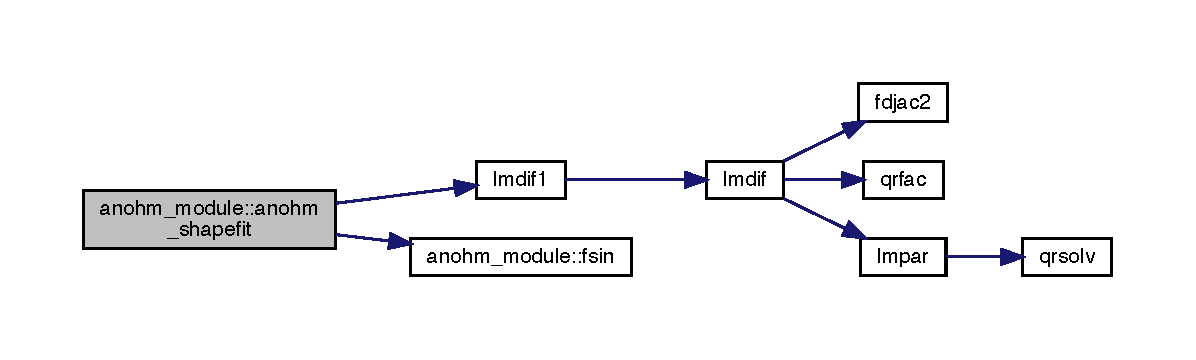
\includegraphics[width=350pt]{namespaceanohm__module_aec263fe8fda2e14111cd3f27a607cff0_cgraph}
\end{center}
\end{figure}
\mbox{\Hypertarget{namespaceanohm__module_a3f1a576bdde691f251c98f56d28b6c5e}\label{namespaceanohm__module_a3f1a576bdde691f251c98f56d28b6c5e}} 
\index{anohm\+\_\+module@{anohm\+\_\+module}!anohm\+\_\+tsurf\+\_\+land\+\_\+cal@{anohm\+\_\+tsurf\+\_\+land\+\_\+cal}}
\index{anohm\+\_\+tsurf\+\_\+land\+\_\+cal@{anohm\+\_\+tsurf\+\_\+land\+\_\+cal}!anohm\+\_\+module@{anohm\+\_\+module}}
\subsubsection{\texorpdfstring{anohm\+\_\+tsurf\+\_\+land\+\_\+cal()}{anohm\_tsurf\_land\_cal()}}
{\footnotesize\ttfamily subroutine anohm\+\_\+module\+::anohm\+\_\+tsurf\+\_\+land\+\_\+cal (\begin{DoxyParamCaption}\item[{real(kind(1d0)), intent(in)}]{A\+Sd,  }\item[{real(kind(1d0)), intent(in)}]{m\+Sd,  }\item[{real(kind(1d0)), intent(in)}]{A\+Ta,  }\item[{real(kind(1d0)), intent(in)}]{m\+Ta,  }\item[{real(kind(1d0)), intent(in)}]{tau,  }\item[{real(kind(1d0)), intent(in)}]{m\+WS,  }\item[{real(kind(1d0)), intent(in)}]{m\+WF,  }\item[{real(kind(1d0)), intent(in)}]{m\+AH,  }\item[{real(kind(1d0)), intent(in)}]{xalb,  }\item[{real(kind(1d0)), intent(in)}]{xemis,  }\item[{real(kind(1d0)), intent(in)}]{xcp,  }\item[{real(kind(1d0)), intent(in)}]{xk,  }\item[{real(kind(1d0)), intent(in)}]{xch,  }\item[{real(kind(1d0)), intent(in)}]{x\+Bo,  }\item[{real(kind(1d0)), intent(out)}]{A\+Ts,  }\item[{real(kind(1d0)), intent(out)}]{m\+Ts,  }\item[{real(kind(1d0)), intent(out)}]{gamma }\end{DoxyParamCaption})}



a wrapper for calculating surface temperature scales 

\begin{DoxyReturn}{Returns}

\begin{DoxyEnumerate}
\item A\+Ts coefficients of a given surface type\+: a1, a2 and a3
\item m\+Ts coefficients of a given surface type\+: a1, a2 and a3
\item gamma coefficients of a given surface type\+: a1, a2 and a3
\end{DoxyEnumerate}
\end{DoxyReturn}

\begin{DoxyParams}[1]{Parameters}
\mbox{\tt in}  & {\em asd} & daily amplitude of solar radiation\\
\hline
\mbox{\tt in}  & {\em msd} & daily mean solar radiation\\
\hline
\mbox{\tt in}  & {\em ata} & daily amplitude of air temperature\\
\hline
\mbox{\tt in}  & {\em mta} & daily mean air temperature\\
\hline
\mbox{\tt in}  & {\em tau} & phase lag between Sd and Ta (Ta-\/\+Sd)\\
\hline
\mbox{\tt in}  & {\em mws} & daily mean wind speed\\
\hline
\mbox{\tt in}  & {\em mwf} & daily mean underground moisture flux\\
\hline
\mbox{\tt in}  & {\em mah} & daily mean anthropogenic heat flux\\
\hline
\mbox{\tt in}  & {\em xalb} & albedo\\
\hline
\mbox{\tt in}  & {\em xemis} & emissivity\\
\hline
\mbox{\tt in}  & {\em xcp} & heat capacity\\
\hline
\mbox{\tt in}  & {\em xk} & thermal conductivity\\
\hline
\mbox{\tt in}  & {\em xch} & bulk transfer coef\\
\hline
\mbox{\tt in}  & {\em xbo} & Bowen ratio\\
\hline
\mbox{\tt out}  & {\em ats} & a1\\
\hline
\mbox{\tt out}  & {\em mts} & a2\\
\hline
\mbox{\tt out}  & {\em gamma} & a3 \\
\hline
\end{DoxyParams}


Definition at line 358 of file S\+U\+E\+W\+S\+\_\+\+An\+O\+H\+M.\+f95.

Here is the call graph for this function\+:\nopagebreak
\begin{figure}[H]
\begin{center}
\leavevmode
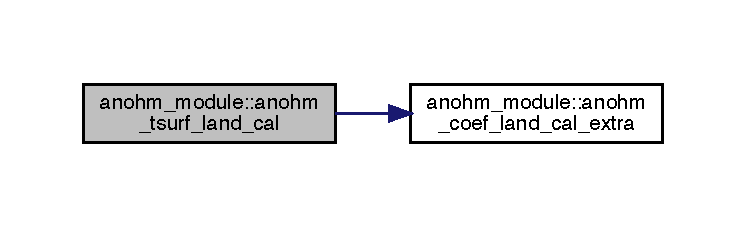
\includegraphics[width=350pt]{namespaceanohm__module_a3f1a576bdde691f251c98f56d28b6c5e_cgraph}
\end{center}
\end{figure}
\mbox{\Hypertarget{namespaceanohm__module_a54c27af87baa1736fd40590bed6c081e}\label{namespaceanohm__module_a54c27af87baa1736fd40590bed6c081e}} 
\index{anohm\+\_\+module@{anohm\+\_\+module}!anohm\+\_\+xts@{anohm\+\_\+xts}}
\index{anohm\+\_\+xts@{anohm\+\_\+xts}!anohm\+\_\+module@{anohm\+\_\+module}}
\subsubsection{\texorpdfstring{anohm\+\_\+xts()}{anohm\_xts()}}
{\footnotesize\ttfamily subroutine anohm\+\_\+module\+::anohm\+\_\+xts (\begin{DoxyParamCaption}\item[{real(kind(1d0)), intent(in)}]{A\+Sd,  }\item[{real(kind(1d0)), intent(in)}]{m\+Sd,  }\item[{real(kind(1d0)), intent(in)}]{A\+Ta,  }\item[{real(kind(1d0)), intent(in)}]{m\+Ta,  }\item[{real(kind(1d0)), intent(in)}]{tau,  }\item[{real(kind(1d0)), intent(in)}]{m\+WS,  }\item[{real(kind(1d0)), intent(in)}]{m\+WF,  }\item[{real(kind(1d0)), intent(in)}]{m\+AH,  }\item[{real(kind(1d0)), intent(in)}]{xalb,  }\item[{real(kind(1d0)), intent(in)}]{xemis,  }\item[{real(kind(1d0)), intent(in)}]{xcp,  }\item[{real(kind(1d0)), intent(in)}]{xk,  }\item[{real(kind(1d0)), intent(in)}]{xch,  }\item[{real(kind(1d0)), intent(in)}]{x\+Bo,  }\item[{real(kind(1d0)), intent(in)}]{t\+Sd,  }\item[{real(kind(1d0)), intent(in)}]{x\+T\+Hr,  }\item[{real(kind(1d0)), intent(out)}]{x\+Ts }\end{DoxyParamCaption})}



calculate the surface temperature related parameters (A\+Ts, m\+Ts, gamma) based on forcings and sfc. conditions 

\begin{DoxyReturn}{Returns}
{\bfseries x\+Ts} surface temperature at local time
\end{DoxyReturn}

\begin{DoxyParams}[1]{Parameters}
\mbox{\tt in}  & {\em asd} & daily amplitude of solar radiation\\
\hline
\mbox{\tt in}  & {\em msd} & daily mean solar radiation\\
\hline
\mbox{\tt in}  & {\em ata} & daily amplitude of air temperature\\
\hline
\mbox{\tt in}  & {\em mta} & daily mean air temperature\\
\hline
\mbox{\tt in}  & {\em tau} & phase lag between Sd and Ta (Ta-\/\+Sd)\\
\hline
\mbox{\tt in}  & {\em mws} & daily mean wind speed\\
\hline
\mbox{\tt in}  & {\em mwf} & daily mean underground moisture flux\\
\hline
\mbox{\tt in}  & {\em mah} & daily mean anthropogenic heat flux\\
\hline
\mbox{\tt in}  & {\em xalb} & albedo\\
\hline
\mbox{\tt in}  & {\em xemis} & emissivity\\
\hline
\mbox{\tt in}  & {\em xcp} & heat capacity\\
\hline
\mbox{\tt in}  & {\em xk} & thermal conductivity\\
\hline
\mbox{\tt in}  & {\em xch} & bulk transfer coef\\
\hline
\mbox{\tt in}  & {\em xbo} & Bowen ratio\\
\hline
\mbox{\tt in}  & {\em tsd} & local peaking time of Sd, hour\\
\hline
\mbox{\tt in}  & {\em xthr} & local time to calculate Ts, hour\\
\hline
\mbox{\tt out}  & {\em xts} & surface temperature at x\+T\+Hr(hr) \\
\hline
\end{DoxyParams}


Definition at line 411 of file S\+U\+E\+W\+S\+\_\+\+An\+O\+H\+M.\+f95.

Here is the call graph for this function\+:\nopagebreak
\begin{figure}[H]
\begin{center}
\leavevmode
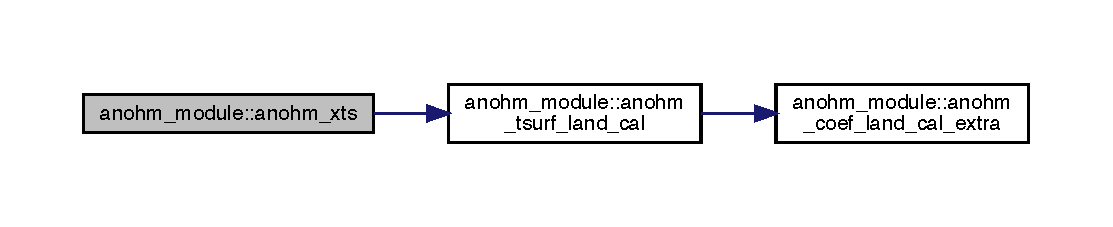
\includegraphics[width=350pt]{namespaceanohm__module_a54c27af87baa1736fd40590bed6c081e_cgraph}
\end{center}
\end{figure}
\mbox{\Hypertarget{namespaceanohm__module_a6111dd73f21e92071faa29d426ae84f9}\label{namespaceanohm__module_a6111dd73f21e92071faa29d426ae84f9}} 
\index{anohm\+\_\+module@{anohm\+\_\+module}!fcnbo@{fcnbo}}
\index{fcnbo@{fcnbo}!anohm\+\_\+module@{anohm\+\_\+module}}
\subsubsection{\texorpdfstring{fcnbo()}{fcnbo()}}
{\footnotesize\ttfamily subroutine anohm\+\_\+module\+::fcnbo (\begin{DoxyParamCaption}\item[{integer ( kind = 4 )}]{n,  }\item[{real ( kind = 8 ), dimension(n)}]{x,  }\item[{real ( kind = 8 ), dimension(n)}]{fvec,  }\item[{integer ( kind = 4 )}]{iflag }\end{DoxyParamCaption})}



this fucntion will construct an equaiton for Bo calculation 



Definition at line 1473 of file S\+U\+E\+W\+S\+\_\+\+An\+O\+H\+M.\+f95.

Here is the call graph for this function\+:\nopagebreak
\begin{figure}[H]
\begin{center}
\leavevmode
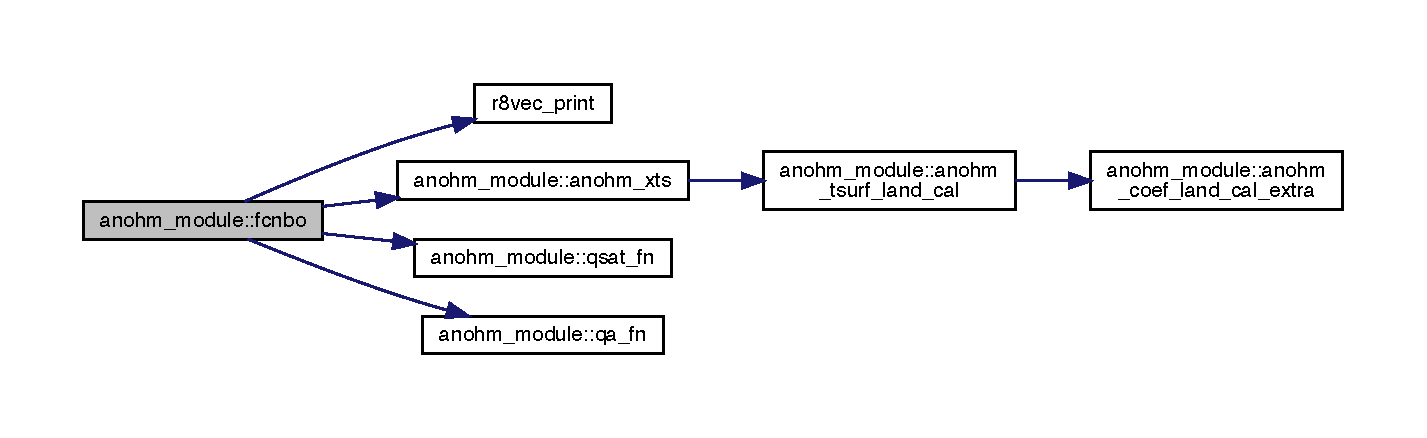
\includegraphics[width=350pt]{namespaceanohm__module_a6111dd73f21e92071faa29d426ae84f9_cgraph}
\end{center}
\end{figure}
\mbox{\Hypertarget{namespaceanohm__module_a8d56836cb99e49028266fac2beaf5b95}\label{namespaceanohm__module_a8d56836cb99e49028266fac2beaf5b95}} 
\index{anohm\+\_\+module@{anohm\+\_\+module}!fsin@{fsin}}
\index{fsin@{fsin}!anohm\+\_\+module@{anohm\+\_\+module}}
\subsubsection{\texorpdfstring{fsin()}{fsin()}}
{\footnotesize\ttfamily subroutine anohm\+\_\+module\+::fsin (\begin{DoxyParamCaption}\item[{integer ( kind = 4 )}]{m,  }\item[{integer ( kind = 4 )}]{n,  }\item[{real ( kind = 8 ), dimension(n)}]{x,  }\item[{real ( kind = 8 ), dimension(m)}]{xdat,  }\item[{real ( kind = 8 ), dimension(m)}]{ydat,  }\item[{real ( kind = 8 ), dimension(m)}]{fvec,  }\item[{integer ( kind = 4 )}]{iflag }\end{DoxyParamCaption})}



sinusoidal function f(t) for fitting\+: f(t) = mean+amp$\ast$\+Sin(Pi/12(t-\/delta)) x = (/mean,amp,delta/) contains the fitting parameters 



Definition at line 1252 of file S\+U\+E\+W\+S\+\_\+\+An\+O\+H\+M.\+f95.

\mbox{\Hypertarget{namespaceanohm__module_ac9feb33254cb5595d19ad7f8a012ef92}\label{namespaceanohm__module_ac9feb33254cb5595d19ad7f8a012ef92}} 
\index{anohm\+\_\+module@{anohm\+\_\+module}!qa\+\_\+fn@{qa\+\_\+fn}}
\index{qa\+\_\+fn@{qa\+\_\+fn}!anohm\+\_\+module@{anohm\+\_\+module}}
\subsubsection{\texorpdfstring{qa\+\_\+fn()}{qa\_fn()}}
{\footnotesize\ttfamily real (kind(1d0)) function anohm\+\_\+module\+::qa\+\_\+fn (\begin{DoxyParamCaption}\item[{real (kind(1d0))}]{Ta,  }\item[{real (kind(1d0))}]{RH,  }\item[{real (kind(1d0))}]{pres }\end{DoxyParamCaption})}



convert relative humidity (RH) to specific humidity (qa) at air temperature (Ta) and atmospheric pressure (pres) 



Definition at line 1660 of file S\+U\+E\+W\+S\+\_\+\+An\+O\+H\+M.\+f95.

\mbox{\Hypertarget{namespaceanohm__module_a0db1439a632619dd005b69ce0fcb9cbe}\label{namespaceanohm__module_a0db1439a632619dd005b69ce0fcb9cbe}} 
\index{anohm\+\_\+module@{anohm\+\_\+module}!qsat\+\_\+fn@{qsat\+\_\+fn}}
\index{qsat\+\_\+fn@{qsat\+\_\+fn}!anohm\+\_\+module@{anohm\+\_\+module}}
\subsubsection{\texorpdfstring{qsat\+\_\+fn()}{qsat\_fn()}}
{\footnotesize\ttfamily real (kind(1d0)) function anohm\+\_\+module\+::qsat\+\_\+fn (\begin{DoxyParamCaption}\item[{real (kind(1d0))}]{Ta,  }\item[{real (kind(1d0))}]{pres }\end{DoxyParamCaption})}



calculate saturation specific humidity (qsat) at air temperature (Ta) and atmospheric pressure (pres) 



Definition at line 1639 of file S\+U\+E\+W\+S\+\_\+\+An\+O\+H\+M.\+f95.


\hypertarget{namespacecbl__module}{}\section{cbl\+\_\+module Module Reference}
\label{namespacecbl__module}\index{cbl\+\_\+module@{cbl\+\_\+module}}
\subsection*{Variables}
\begin{DoxyCompactItemize}
\item 
integer \hyperlink{namespacecbl__module_a904519e3dcaa1592e2506c840b8cc7e4}{entrainmenttype}
\item 
integer \hyperlink{namespacecbl__module_a1fe4af3f4b8ea35de69189177bcc9d5d}{co2\+\_\+included}
\item 
integer \hyperlink{namespacecbl__module_ad06cbd2f8723521c7d20e7d57ebe0f9c}{initialdata\+\_\+use}
\item 
integer \hyperlink{namespacecbl__module_a546f4ac8b1d6305356caf940d8e8e342}{sondeflag}
\item 
integer \hyperlink{namespacecbl__module_a0140016345794a8912c00aafaf50fe1e}{isubs}
\item 
integer, dimension(366) \hyperlink{namespacecbl__module_a5901bc487fe54be32f04988c42ab7443}{cblday} =0
\item 
character(len=200), dimension(366) \hyperlink{namespacecbl__module_a810011542edd41ab403379b2004c84ab}{filesonde} =\char`\"{}\char`\"{}
\item 
character(len=200) \hyperlink{namespacecbl__module_add8682c29dcc92f528e2894dd1e16f39}{initialdatafilename}
\item 
real(kind(1d0)) \hyperlink{namespacecbl__module_acdfa6106091fdfa93a6cab25af3d0f1a}{wsb}
\item 
real(kind(1d0)), dimension(1\+:10) \hyperlink{namespacecbl__module_aae12ee171bb6806332a07b9300284693}{cbldata}
\item 
real(kind(1d0)), dimension(\+:,\+:), allocatable \hyperlink{namespacecbl__module_ae82d92a08db006da8495afa687a74c6c}{inicbldata}
\item 
integer \hyperlink{namespacecbl__module_ad6ee0356644a1bc5acc13c4dc71ad4f9}{zmax}
\item 
integer \hyperlink{namespacecbl__module_a52c76c9e4368adec7890e95932374f73}{neqn} =6
\item 
integer \hyperlink{namespacecbl__module_a105bb269b58c37d9b6170f7aa3a74fbe}{icblcount}
\item 
integer \hyperlink{namespacecbl__module_a5f768f5aae74fa7b0c2d66118fc71ba5}{nlineindata}
\item 
real(kind(1d0)) \hyperlink{namespacecbl__module_a295b5b9a6a2d8808cba5c386dd4ed2e6}{c2k} =273.\+16
\item 
real(kind(1d0)) \hyperlink{namespacecbl__module_ac165fc78c97d6f5f81b06c8282165aa0}{usbl}
\item 
real(kind(1d0)) \hyperlink{namespacecbl__module_a9096ed1c586fe2526affe44bdc6a3506}{ftbl}
\item 
real(kind(1d0)) \hyperlink{namespacecbl__module_a976e376b24178298356c3ffba35082f8}{fqbl}
\item 
real(kind(1d0)) \hyperlink{namespacecbl__module_abece0fd4503899af7cb75b51be8b5e63}{fcbl}
\item 
real(kind(1d0)) \hyperlink{namespacecbl__module_ab55715333b9dc4e5699d418ce9aa6eca}{gamt}
\item 
real(kind(1d0)) \hyperlink{namespacecbl__module_a2f0b130ab9a329454293c11707b4f89f}{gamq}
\item 
real(kind(1d0)) \hyperlink{namespacecbl__module_a999c82d729d623cf9e734d5b8f60413b}{gamc}
\item 
real(kind(1d0)) \hyperlink{namespacecbl__module_a32c6cd32a6011ce9ce3536df1935b6ba}{tpp}
\item 
real(kind(1d0)) \hyperlink{namespacecbl__module_a532658820cffbe2b75b727fb9e55d779}{qpp}
\item 
real(kind(1d0)) \hyperlink{namespacecbl__module_a01651700bba3680529190559891e308f}{cp0}
\item 
real(kind(1d0)) \hyperlink{namespacecbl__module_ab09c1f0f6b67d7bdf17278e617fc35ba}{alpha3}
\item 
real(kind(1d0)) \hyperlink{namespacecbl__module_a20477a72c625deb14eccf5e2cd767d95}{blh\+\_\+m}
\item 
real(kind(1d0)) \hyperlink{namespacecbl__module_a19dd722436e710830c7ff6b961753c62}{blh1\+\_\+m}
\item 
real(kind(1d0)) \hyperlink{namespacecbl__module_ab5d6f31d2f9b523336fb0947a1e53707}{cm}
\item 
real(kind(1d0)) \hyperlink{namespacecbl__module_a86a03f05040f82f59951951ed8feb92d}{gamt\+\_\+km}
\item 
real(kind(1d0)) \hyperlink{namespacecbl__module_a6aab251dd8f51c9cd6a8dc723a99fdf3}{gamq\+\_\+gkgm}
\item 
real(kind(1d0)) \hyperlink{namespacecbl__module_a1ce0de96513d92e7be4a7b0318a7102a}{gamq\+\_\+kgkgm}
\item 
real(kind(1d0)) \hyperlink{namespacecbl__module_a9981080497583b5953927b0a2bbdcde8}{tm\+\_\+c}
\item 
real(kind(1d0)) \hyperlink{namespacecbl__module_afb21accdfbc0b24e12b24a44ffd9d6d1}{tm\+\_\+k}
\item 
real(kind(1d0)) \hyperlink{namespacecbl__module_a8cbccf2c4274c8e254bdd331947d39b8}{tmp\+\_\+k}
\item 
real(kind(1d0)) \hyperlink{namespacecbl__module_a7b92d87a613cb13145b7c84beced7f67}{tp\+\_\+c}
\item 
real(kind(1d0)) \hyperlink{namespacecbl__module_af9b1b9c8cf1a15dca9b8750920a048c3}{tp\+\_\+k}
\item 
real(kind(1d0)) \hyperlink{namespacecbl__module_a63c8fb6ebf38a621ec616ddb04445f03}{tpp\+\_\+k}
\item 
real(kind(1d0)) \hyperlink{namespacecbl__module_a5b2329a6a103326f5fa08282787d83aa}{febl\+\_\+kgkgms}
\item 
real(kind(1d0)) \hyperlink{namespacecbl__module_a3bb0811c2c1eb194eff7132bb1a906ef}{fhbl\+\_\+kms}
\item 
real(kind(1d0)) \hyperlink{namespacecbl__module_a652625bc960f05e00df2f7bf48cb7444}{qm\+\_\+gkg}
\item 
real(kind(1d0)) \hyperlink{namespacecbl__module_aa9e98a57d9be62a92919841c4ad428b9}{qm\+\_\+kgkg}
\item 
real(kind(1d0)) \hyperlink{namespacecbl__module_a45208115b84dad98c55d11cf93307c0c}{qp\+\_\+gkg}
\item 
real(kind(1d0)) \hyperlink{namespacecbl__module_a19585b12b6f9726bfbda1954703b7b4d}{qp\+\_\+kgkg}
\item 
real(kind(1d0)) \hyperlink{namespacecbl__module_a9698f773fdba998c463aa4dad50675a6}{qpp\+\_\+kgkg}
\item 
real(kind(1d0)), dimension(0\+:500, 2) \hyperlink{namespacecbl__module_aa6c88eb40ac8bd6e5a7df04080288218}{gtheta}
\item 
real(kind(1d0)), dimension(0\+:500, 2) \hyperlink{namespacecbl__module_a2c8e164b18520600e084ab16825b7996}{ghum}
\item 
real(kind(1d0)), dimension(6) \hyperlink{namespacecbl__module_a3d7f7d5671cd679f69c81da2fbf797e2}{y}
\end{DoxyCompactItemize}


\subsection{Variable Documentation}
\mbox{\Hypertarget{namespacecbl__module_ab09c1f0f6b67d7bdf17278e617fc35ba}\label{namespacecbl__module_ab09c1f0f6b67d7bdf17278e617fc35ba}} 
\index{cbl\+\_\+module@{cbl\+\_\+module}!alpha3@{alpha3}}
\index{alpha3@{alpha3}!cbl\+\_\+module@{cbl\+\_\+module}}
\subsubsection{\texorpdfstring{alpha3}{alpha3}}
{\footnotesize\ttfamily real(kind(1d0)) cbl\+\_\+module\+::alpha3}



Definition at line 1063 of file L\+U\+M\+P\+S\+\_\+\+Module\+\_\+constants.\+f95.

\mbox{\Hypertarget{namespacecbl__module_a19dd722436e710830c7ff6b961753c62}\label{namespacecbl__module_a19dd722436e710830c7ff6b961753c62}} 
\index{cbl\+\_\+module@{cbl\+\_\+module}!blh1\+\_\+m@{blh1\+\_\+m}}
\index{blh1\+\_\+m@{blh1\+\_\+m}!cbl\+\_\+module@{cbl\+\_\+module}}
\subsubsection{\texorpdfstring{blh1\+\_\+m}{blh1\_m}}
{\footnotesize\ttfamily real(kind(1d0)) cbl\+\_\+module\+::blh1\+\_\+m}



Definition at line 1063 of file L\+U\+M\+P\+S\+\_\+\+Module\+\_\+constants.\+f95.

\mbox{\Hypertarget{namespacecbl__module_a20477a72c625deb14eccf5e2cd767d95}\label{namespacecbl__module_a20477a72c625deb14eccf5e2cd767d95}} 
\index{cbl\+\_\+module@{cbl\+\_\+module}!blh\+\_\+m@{blh\+\_\+m}}
\index{blh\+\_\+m@{blh\+\_\+m}!cbl\+\_\+module@{cbl\+\_\+module}}
\subsubsection{\texorpdfstring{blh\+\_\+m}{blh\_m}}
{\footnotesize\ttfamily real(kind(1d0)) cbl\+\_\+module\+::blh\+\_\+m}



Definition at line 1063 of file L\+U\+M\+P\+S\+\_\+\+Module\+\_\+constants.\+f95.

\mbox{\Hypertarget{namespacecbl__module_a295b5b9a6a2d8808cba5c386dd4ed2e6}\label{namespacecbl__module_a295b5b9a6a2d8808cba5c386dd4ed2e6}} 
\index{cbl\+\_\+module@{cbl\+\_\+module}!c2k@{c2k}}
\index{c2k@{c2k}!cbl\+\_\+module@{cbl\+\_\+module}}
\subsubsection{\texorpdfstring{c2k}{c2k}}
{\footnotesize\ttfamily real(kind(1d0)) cbl\+\_\+module\+::c2k =273.\+16}



Definition at line 1059 of file L\+U\+M\+P\+S\+\_\+\+Module\+\_\+constants.\+f95.

\mbox{\Hypertarget{namespacecbl__module_aae12ee171bb6806332a07b9300284693}\label{namespacecbl__module_aae12ee171bb6806332a07b9300284693}} 
\index{cbl\+\_\+module@{cbl\+\_\+module}!cbldata@{cbldata}}
\index{cbldata@{cbldata}!cbl\+\_\+module@{cbl\+\_\+module}}
\subsubsection{\texorpdfstring{cbldata}{cbldata}}
{\footnotesize\ttfamily real(kind(1d0)), dimension(1\+:10) cbl\+\_\+module\+::cbldata}



Definition at line 1051 of file L\+U\+M\+P\+S\+\_\+\+Module\+\_\+constants.\+f95.

\mbox{\Hypertarget{namespacecbl__module_a5901bc487fe54be32f04988c42ab7443}\label{namespacecbl__module_a5901bc487fe54be32f04988c42ab7443}} 
\index{cbl\+\_\+module@{cbl\+\_\+module}!cblday@{cblday}}
\index{cblday@{cblday}!cbl\+\_\+module@{cbl\+\_\+module}}
\subsubsection{\texorpdfstring{cblday}{cblday}}
{\footnotesize\ttfamily integer, dimension(366) cbl\+\_\+module\+::cblday =0}



Definition at line 1046 of file L\+U\+M\+P\+S\+\_\+\+Module\+\_\+constants.\+f95.

\mbox{\Hypertarget{namespacecbl__module_ab5d6f31d2f9b523336fb0947a1e53707}\label{namespacecbl__module_ab5d6f31d2f9b523336fb0947a1e53707}} 
\index{cbl\+\_\+module@{cbl\+\_\+module}!cm@{cm}}
\index{cm@{cm}!cbl\+\_\+module@{cbl\+\_\+module}}
\subsubsection{\texorpdfstring{cm}{cm}}
{\footnotesize\ttfamily real(kind(1d0)) cbl\+\_\+module\+::cm}



Definition at line 1063 of file L\+U\+M\+P\+S\+\_\+\+Module\+\_\+constants.\+f95.

\mbox{\Hypertarget{namespacecbl__module_a1fe4af3f4b8ea35de69189177bcc9d5d}\label{namespacecbl__module_a1fe4af3f4b8ea35de69189177bcc9d5d}} 
\index{cbl\+\_\+module@{cbl\+\_\+module}!co2\+\_\+included@{co2\+\_\+included}}
\index{co2\+\_\+included@{co2\+\_\+included}!cbl\+\_\+module@{cbl\+\_\+module}}
\subsubsection{\texorpdfstring{co2\+\_\+included}{co2\_included}}
{\footnotesize\ttfamily integer cbl\+\_\+module\+::co2\+\_\+included}



Definition at line 1039 of file L\+U\+M\+P\+S\+\_\+\+Module\+\_\+constants.\+f95.

\mbox{\Hypertarget{namespacecbl__module_a01651700bba3680529190559891e308f}\label{namespacecbl__module_a01651700bba3680529190559891e308f}} 
\index{cbl\+\_\+module@{cbl\+\_\+module}!cp0@{cp0}}
\index{cp0@{cp0}!cbl\+\_\+module@{cbl\+\_\+module}}
\subsubsection{\texorpdfstring{cp0}{cp0}}
{\footnotesize\ttfamily real (kind(1d0)) cbl\+\_\+module\+::cp0}



Definition at line 1061 of file L\+U\+M\+P\+S\+\_\+\+Module\+\_\+constants.\+f95.

\mbox{\Hypertarget{namespacecbl__module_a904519e3dcaa1592e2506c840b8cc7e4}\label{namespacecbl__module_a904519e3dcaa1592e2506c840b8cc7e4}} 
\index{cbl\+\_\+module@{cbl\+\_\+module}!entrainmenttype@{entrainmenttype}}
\index{entrainmenttype@{entrainmenttype}!cbl\+\_\+module@{cbl\+\_\+module}}
\subsubsection{\texorpdfstring{entrainmenttype}{entrainmenttype}}
{\footnotesize\ttfamily integer cbl\+\_\+module\+::entrainmenttype}



Definition at line 1039 of file L\+U\+M\+P\+S\+\_\+\+Module\+\_\+constants.\+f95.

\mbox{\Hypertarget{namespacecbl__module_abece0fd4503899af7cb75b51be8b5e63}\label{namespacecbl__module_abece0fd4503899af7cb75b51be8b5e63}} 
\index{cbl\+\_\+module@{cbl\+\_\+module}!fcbl@{fcbl}}
\index{fcbl@{fcbl}!cbl\+\_\+module@{cbl\+\_\+module}}
\subsubsection{\texorpdfstring{fcbl}{fcbl}}
{\footnotesize\ttfamily real (kind(1d0)) cbl\+\_\+module\+::fcbl}



Definition at line 1061 of file L\+U\+M\+P\+S\+\_\+\+Module\+\_\+constants.\+f95.

\mbox{\Hypertarget{namespacecbl__module_a5b2329a6a103326f5fa08282787d83aa}\label{namespacecbl__module_a5b2329a6a103326f5fa08282787d83aa}} 
\index{cbl\+\_\+module@{cbl\+\_\+module}!febl\+\_\+kgkgms@{febl\+\_\+kgkgms}}
\index{febl\+\_\+kgkgms@{febl\+\_\+kgkgms}!cbl\+\_\+module@{cbl\+\_\+module}}
\subsubsection{\texorpdfstring{febl\+\_\+kgkgms}{febl\_kgkgms}}
{\footnotesize\ttfamily real(kind(1d0)) cbl\+\_\+module\+::febl\+\_\+kgkgms}



Definition at line 1063 of file L\+U\+M\+P\+S\+\_\+\+Module\+\_\+constants.\+f95.

\mbox{\Hypertarget{namespacecbl__module_a3bb0811c2c1eb194eff7132bb1a906ef}\label{namespacecbl__module_a3bb0811c2c1eb194eff7132bb1a906ef}} 
\index{cbl\+\_\+module@{cbl\+\_\+module}!fhbl\+\_\+kms@{fhbl\+\_\+kms}}
\index{fhbl\+\_\+kms@{fhbl\+\_\+kms}!cbl\+\_\+module@{cbl\+\_\+module}}
\subsubsection{\texorpdfstring{fhbl\+\_\+kms}{fhbl\_kms}}
{\footnotesize\ttfamily real(kind(1d0)) cbl\+\_\+module\+::fhbl\+\_\+kms}



Definition at line 1063 of file L\+U\+M\+P\+S\+\_\+\+Module\+\_\+constants.\+f95.

\mbox{\Hypertarget{namespacecbl__module_a810011542edd41ab403379b2004c84ab}\label{namespacecbl__module_a810011542edd41ab403379b2004c84ab}} 
\index{cbl\+\_\+module@{cbl\+\_\+module}!filesonde@{filesonde}}
\index{filesonde@{filesonde}!cbl\+\_\+module@{cbl\+\_\+module}}
\subsubsection{\texorpdfstring{filesonde}{filesonde}}
{\footnotesize\ttfamily character (len=200), dimension(366) cbl\+\_\+module\+::filesonde =\char`\"{}\char`\"{}}



Definition at line 1048 of file L\+U\+M\+P\+S\+\_\+\+Module\+\_\+constants.\+f95.

\mbox{\Hypertarget{namespacecbl__module_a976e376b24178298356c3ffba35082f8}\label{namespacecbl__module_a976e376b24178298356c3ffba35082f8}} 
\index{cbl\+\_\+module@{cbl\+\_\+module}!fqbl@{fqbl}}
\index{fqbl@{fqbl}!cbl\+\_\+module@{cbl\+\_\+module}}
\subsubsection{\texorpdfstring{fqbl}{fqbl}}
{\footnotesize\ttfamily real (kind(1d0)) cbl\+\_\+module\+::fqbl}



Definition at line 1061 of file L\+U\+M\+P\+S\+\_\+\+Module\+\_\+constants.\+f95.

\mbox{\Hypertarget{namespacecbl__module_a9096ed1c586fe2526affe44bdc6a3506}\label{namespacecbl__module_a9096ed1c586fe2526affe44bdc6a3506}} 
\index{cbl\+\_\+module@{cbl\+\_\+module}!ftbl@{ftbl}}
\index{ftbl@{ftbl}!cbl\+\_\+module@{cbl\+\_\+module}}
\subsubsection{\texorpdfstring{ftbl}{ftbl}}
{\footnotesize\ttfamily real (kind(1d0)) cbl\+\_\+module\+::ftbl}



Definition at line 1061 of file L\+U\+M\+P\+S\+\_\+\+Module\+\_\+constants.\+f95.

\mbox{\Hypertarget{namespacecbl__module_a999c82d729d623cf9e734d5b8f60413b}\label{namespacecbl__module_a999c82d729d623cf9e734d5b8f60413b}} 
\index{cbl\+\_\+module@{cbl\+\_\+module}!gamc@{gamc}}
\index{gamc@{gamc}!cbl\+\_\+module@{cbl\+\_\+module}}
\subsubsection{\texorpdfstring{gamc}{gamc}}
{\footnotesize\ttfamily real (kind(1d0)) cbl\+\_\+module\+::gamc}



Definition at line 1061 of file L\+U\+M\+P\+S\+\_\+\+Module\+\_\+constants.\+f95.

\mbox{\Hypertarget{namespacecbl__module_a2f0b130ab9a329454293c11707b4f89f}\label{namespacecbl__module_a2f0b130ab9a329454293c11707b4f89f}} 
\index{cbl\+\_\+module@{cbl\+\_\+module}!gamq@{gamq}}
\index{gamq@{gamq}!cbl\+\_\+module@{cbl\+\_\+module}}
\subsubsection{\texorpdfstring{gamq}{gamq}}
{\footnotesize\ttfamily real (kind(1d0)) cbl\+\_\+module\+::gamq}



Definition at line 1061 of file L\+U\+M\+P\+S\+\_\+\+Module\+\_\+constants.\+f95.

\mbox{\Hypertarget{namespacecbl__module_a6aab251dd8f51c9cd6a8dc723a99fdf3}\label{namespacecbl__module_a6aab251dd8f51c9cd6a8dc723a99fdf3}} 
\index{cbl\+\_\+module@{cbl\+\_\+module}!gamq\+\_\+gkgm@{gamq\+\_\+gkgm}}
\index{gamq\+\_\+gkgm@{gamq\+\_\+gkgm}!cbl\+\_\+module@{cbl\+\_\+module}}
\subsubsection{\texorpdfstring{gamq\+\_\+gkgm}{gamq\_gkgm}}
{\footnotesize\ttfamily real(kind(1d0)) cbl\+\_\+module\+::gamq\+\_\+gkgm}



Definition at line 1063 of file L\+U\+M\+P\+S\+\_\+\+Module\+\_\+constants.\+f95.

\mbox{\Hypertarget{namespacecbl__module_a1ce0de96513d92e7be4a7b0318a7102a}\label{namespacecbl__module_a1ce0de96513d92e7be4a7b0318a7102a}} 
\index{cbl\+\_\+module@{cbl\+\_\+module}!gamq\+\_\+kgkgm@{gamq\+\_\+kgkgm}}
\index{gamq\+\_\+kgkgm@{gamq\+\_\+kgkgm}!cbl\+\_\+module@{cbl\+\_\+module}}
\subsubsection{\texorpdfstring{gamq\+\_\+kgkgm}{gamq\_kgkgm}}
{\footnotesize\ttfamily real(kind(1d0)) cbl\+\_\+module\+::gamq\+\_\+kgkgm}



Definition at line 1063 of file L\+U\+M\+P\+S\+\_\+\+Module\+\_\+constants.\+f95.

\mbox{\Hypertarget{namespacecbl__module_ab55715333b9dc4e5699d418ce9aa6eca}\label{namespacecbl__module_ab55715333b9dc4e5699d418ce9aa6eca}} 
\index{cbl\+\_\+module@{cbl\+\_\+module}!gamt@{gamt}}
\index{gamt@{gamt}!cbl\+\_\+module@{cbl\+\_\+module}}
\subsubsection{\texorpdfstring{gamt}{gamt}}
{\footnotesize\ttfamily real (kind(1d0)) cbl\+\_\+module\+::gamt}



Definition at line 1061 of file L\+U\+M\+P\+S\+\_\+\+Module\+\_\+constants.\+f95.

\mbox{\Hypertarget{namespacecbl__module_a86a03f05040f82f59951951ed8feb92d}\label{namespacecbl__module_a86a03f05040f82f59951951ed8feb92d}} 
\index{cbl\+\_\+module@{cbl\+\_\+module}!gamt\+\_\+km@{gamt\+\_\+km}}
\index{gamt\+\_\+km@{gamt\+\_\+km}!cbl\+\_\+module@{cbl\+\_\+module}}
\subsubsection{\texorpdfstring{gamt\+\_\+km}{gamt\_km}}
{\footnotesize\ttfamily real(kind(1d0)) cbl\+\_\+module\+::gamt\+\_\+km}



Definition at line 1063 of file L\+U\+M\+P\+S\+\_\+\+Module\+\_\+constants.\+f95.

\mbox{\Hypertarget{namespacecbl__module_a2c8e164b18520600e084ab16825b7996}\label{namespacecbl__module_a2c8e164b18520600e084ab16825b7996}} 
\index{cbl\+\_\+module@{cbl\+\_\+module}!ghum@{ghum}}
\index{ghum@{ghum}!cbl\+\_\+module@{cbl\+\_\+module}}
\subsubsection{\texorpdfstring{ghum}{ghum}}
{\footnotesize\ttfamily real (kind(1d0)), dimension (0\+:500,2) cbl\+\_\+module\+::ghum}



Definition at line 1087 of file L\+U\+M\+P\+S\+\_\+\+Module\+\_\+constants.\+f95.

\mbox{\Hypertarget{namespacecbl__module_aa6c88eb40ac8bd6e5a7df04080288218}\label{namespacecbl__module_aa6c88eb40ac8bd6e5a7df04080288218}} 
\index{cbl\+\_\+module@{cbl\+\_\+module}!gtheta@{gtheta}}
\index{gtheta@{gtheta}!cbl\+\_\+module@{cbl\+\_\+module}}
\subsubsection{\texorpdfstring{gtheta}{gtheta}}
{\footnotesize\ttfamily real (kind(1d0)), dimension (0\+:500,2) cbl\+\_\+module\+::gtheta}



Definition at line 1087 of file L\+U\+M\+P\+S\+\_\+\+Module\+\_\+constants.\+f95.

\mbox{\Hypertarget{namespacecbl__module_a105bb269b58c37d9b6170f7aa3a74fbe}\label{namespacecbl__module_a105bb269b58c37d9b6170f7aa3a74fbe}} 
\index{cbl\+\_\+module@{cbl\+\_\+module}!icblcount@{icblcount}}
\index{icblcount@{icblcount}!cbl\+\_\+module@{cbl\+\_\+module}}
\subsubsection{\texorpdfstring{icblcount}{icblcount}}
{\footnotesize\ttfamily integer cbl\+\_\+module\+::icblcount}



Definition at line 1055 of file L\+U\+M\+P\+S\+\_\+\+Module\+\_\+constants.\+f95.

\mbox{\Hypertarget{namespacecbl__module_ae82d92a08db006da8495afa687a74c6c}\label{namespacecbl__module_ae82d92a08db006da8495afa687a74c6c}} 
\index{cbl\+\_\+module@{cbl\+\_\+module}!inicbldata@{inicbldata}}
\index{inicbldata@{inicbldata}!cbl\+\_\+module@{cbl\+\_\+module}}
\subsubsection{\texorpdfstring{inicbldata}{inicbldata}}
{\footnotesize\ttfamily real(kind(1d0)), dimension(\+:,\+:), allocatable cbl\+\_\+module\+::inicbldata}



Definition at line 1052 of file L\+U\+M\+P\+S\+\_\+\+Module\+\_\+constants.\+f95.

\mbox{\Hypertarget{namespacecbl__module_ad06cbd2f8723521c7d20e7d57ebe0f9c}\label{namespacecbl__module_ad06cbd2f8723521c7d20e7d57ebe0f9c}} 
\index{cbl\+\_\+module@{cbl\+\_\+module}!initialdata\+\_\+use@{initialdata\+\_\+use}}
\index{initialdata\+\_\+use@{initialdata\+\_\+use}!cbl\+\_\+module@{cbl\+\_\+module}}
\subsubsection{\texorpdfstring{initialdata\+\_\+use}{initialdata\_use}}
{\footnotesize\ttfamily integer cbl\+\_\+module\+::initialdata\+\_\+use}



Definition at line 1039 of file L\+U\+M\+P\+S\+\_\+\+Module\+\_\+constants.\+f95.

\mbox{\Hypertarget{namespacecbl__module_add8682c29dcc92f528e2894dd1e16f39}\label{namespacecbl__module_add8682c29dcc92f528e2894dd1e16f39}} 
\index{cbl\+\_\+module@{cbl\+\_\+module}!initialdatafilename@{initialdatafilename}}
\index{initialdatafilename@{initialdatafilename}!cbl\+\_\+module@{cbl\+\_\+module}}
\subsubsection{\texorpdfstring{initialdatafilename}{initialdatafilename}}
{\footnotesize\ttfamily character (len=200) cbl\+\_\+module\+::initialdatafilename}



Definition at line 1049 of file L\+U\+M\+P\+S\+\_\+\+Module\+\_\+constants.\+f95.

\mbox{\Hypertarget{namespacecbl__module_a0140016345794a8912c00aafaf50fe1e}\label{namespacecbl__module_a0140016345794a8912c00aafaf50fe1e}} 
\index{cbl\+\_\+module@{cbl\+\_\+module}!isubs@{isubs}}
\index{isubs@{isubs}!cbl\+\_\+module@{cbl\+\_\+module}}
\subsubsection{\texorpdfstring{isubs}{isubs}}
{\footnotesize\ttfamily integer cbl\+\_\+module\+::isubs}



Definition at line 1039 of file L\+U\+M\+P\+S\+\_\+\+Module\+\_\+constants.\+f95.

\mbox{\Hypertarget{namespacecbl__module_a52c76c9e4368adec7890e95932374f73}\label{namespacecbl__module_a52c76c9e4368adec7890e95932374f73}} 
\index{cbl\+\_\+module@{cbl\+\_\+module}!neqn@{neqn}}
\index{neqn@{neqn}!cbl\+\_\+module@{cbl\+\_\+module}}
\subsubsection{\texorpdfstring{neqn}{neqn}}
{\footnotesize\ttfamily integer cbl\+\_\+module\+::neqn =6}



Definition at line 1055 of file L\+U\+M\+P\+S\+\_\+\+Module\+\_\+constants.\+f95.

\mbox{\Hypertarget{namespacecbl__module_a5f768f5aae74fa7b0c2d66118fc71ba5}\label{namespacecbl__module_a5f768f5aae74fa7b0c2d66118fc71ba5}} 
\index{cbl\+\_\+module@{cbl\+\_\+module}!nlineindata@{nlineindata}}
\index{nlineindata@{nlineindata}!cbl\+\_\+module@{cbl\+\_\+module}}
\subsubsection{\texorpdfstring{nlineindata}{nlineindata}}
{\footnotesize\ttfamily integer cbl\+\_\+module\+::nlineindata}



Definition at line 1055 of file L\+U\+M\+P\+S\+\_\+\+Module\+\_\+constants.\+f95.

\mbox{\Hypertarget{namespacecbl__module_a652625bc960f05e00df2f7bf48cb7444}\label{namespacecbl__module_a652625bc960f05e00df2f7bf48cb7444}} 
\index{cbl\+\_\+module@{cbl\+\_\+module}!qm\+\_\+gkg@{qm\+\_\+gkg}}
\index{qm\+\_\+gkg@{qm\+\_\+gkg}!cbl\+\_\+module@{cbl\+\_\+module}}
\subsubsection{\texorpdfstring{qm\+\_\+gkg}{qm\_gkg}}
{\footnotesize\ttfamily real(kind(1d0)) cbl\+\_\+module\+::qm\+\_\+gkg}



Definition at line 1063 of file L\+U\+M\+P\+S\+\_\+\+Module\+\_\+constants.\+f95.

\mbox{\Hypertarget{namespacecbl__module_aa9e98a57d9be62a92919841c4ad428b9}\label{namespacecbl__module_aa9e98a57d9be62a92919841c4ad428b9}} 
\index{cbl\+\_\+module@{cbl\+\_\+module}!qm\+\_\+kgkg@{qm\+\_\+kgkg}}
\index{qm\+\_\+kgkg@{qm\+\_\+kgkg}!cbl\+\_\+module@{cbl\+\_\+module}}
\subsubsection{\texorpdfstring{qm\+\_\+kgkg}{qm\_kgkg}}
{\footnotesize\ttfamily real(kind(1d0)) cbl\+\_\+module\+::qm\+\_\+kgkg}



Definition at line 1063 of file L\+U\+M\+P\+S\+\_\+\+Module\+\_\+constants.\+f95.

\mbox{\Hypertarget{namespacecbl__module_a45208115b84dad98c55d11cf93307c0c}\label{namespacecbl__module_a45208115b84dad98c55d11cf93307c0c}} 
\index{cbl\+\_\+module@{cbl\+\_\+module}!qp\+\_\+gkg@{qp\+\_\+gkg}}
\index{qp\+\_\+gkg@{qp\+\_\+gkg}!cbl\+\_\+module@{cbl\+\_\+module}}
\subsubsection{\texorpdfstring{qp\+\_\+gkg}{qp\_gkg}}
{\footnotesize\ttfamily real(kind(1d0)) cbl\+\_\+module\+::qp\+\_\+gkg}



Definition at line 1063 of file L\+U\+M\+P\+S\+\_\+\+Module\+\_\+constants.\+f95.

\mbox{\Hypertarget{namespacecbl__module_a19585b12b6f9726bfbda1954703b7b4d}\label{namespacecbl__module_a19585b12b6f9726bfbda1954703b7b4d}} 
\index{cbl\+\_\+module@{cbl\+\_\+module}!qp\+\_\+kgkg@{qp\+\_\+kgkg}}
\index{qp\+\_\+kgkg@{qp\+\_\+kgkg}!cbl\+\_\+module@{cbl\+\_\+module}}
\subsubsection{\texorpdfstring{qp\+\_\+kgkg}{qp\_kgkg}}
{\footnotesize\ttfamily real(kind(1d0)) cbl\+\_\+module\+::qp\+\_\+kgkg}



Definition at line 1063 of file L\+U\+M\+P\+S\+\_\+\+Module\+\_\+constants.\+f95.

\mbox{\Hypertarget{namespacecbl__module_a532658820cffbe2b75b727fb9e55d779}\label{namespacecbl__module_a532658820cffbe2b75b727fb9e55d779}} 
\index{cbl\+\_\+module@{cbl\+\_\+module}!qpp@{qpp}}
\index{qpp@{qpp}!cbl\+\_\+module@{cbl\+\_\+module}}
\subsubsection{\texorpdfstring{qpp}{qpp}}
{\footnotesize\ttfamily real (kind(1d0)) cbl\+\_\+module\+::qpp}



Definition at line 1061 of file L\+U\+M\+P\+S\+\_\+\+Module\+\_\+constants.\+f95.

\mbox{\Hypertarget{namespacecbl__module_a9698f773fdba998c463aa4dad50675a6}\label{namespacecbl__module_a9698f773fdba998c463aa4dad50675a6}} 
\index{cbl\+\_\+module@{cbl\+\_\+module}!qpp\+\_\+kgkg@{qpp\+\_\+kgkg}}
\index{qpp\+\_\+kgkg@{qpp\+\_\+kgkg}!cbl\+\_\+module@{cbl\+\_\+module}}
\subsubsection{\texorpdfstring{qpp\+\_\+kgkg}{qpp\_kgkg}}
{\footnotesize\ttfamily real(kind(1d0)) cbl\+\_\+module\+::qpp\+\_\+kgkg}



Definition at line 1063 of file L\+U\+M\+P\+S\+\_\+\+Module\+\_\+constants.\+f95.

\mbox{\Hypertarget{namespacecbl__module_a546f4ac8b1d6305356caf940d8e8e342}\label{namespacecbl__module_a546f4ac8b1d6305356caf940d8e8e342}} 
\index{cbl\+\_\+module@{cbl\+\_\+module}!sondeflag@{sondeflag}}
\index{sondeflag@{sondeflag}!cbl\+\_\+module@{cbl\+\_\+module}}
\subsubsection{\texorpdfstring{sondeflag}{sondeflag}}
{\footnotesize\ttfamily integer cbl\+\_\+module\+::sondeflag}



Definition at line 1039 of file L\+U\+M\+P\+S\+\_\+\+Module\+\_\+constants.\+f95.

\mbox{\Hypertarget{namespacecbl__module_a9981080497583b5953927b0a2bbdcde8}\label{namespacecbl__module_a9981080497583b5953927b0a2bbdcde8}} 
\index{cbl\+\_\+module@{cbl\+\_\+module}!tm\+\_\+c@{tm\+\_\+c}}
\index{tm\+\_\+c@{tm\+\_\+c}!cbl\+\_\+module@{cbl\+\_\+module}}
\subsubsection{\texorpdfstring{tm\+\_\+c}{tm\_c}}
{\footnotesize\ttfamily real(kind(1d0)) cbl\+\_\+module\+::tm\+\_\+c}



Definition at line 1063 of file L\+U\+M\+P\+S\+\_\+\+Module\+\_\+constants.\+f95.

\mbox{\Hypertarget{namespacecbl__module_afb21accdfbc0b24e12b24a44ffd9d6d1}\label{namespacecbl__module_afb21accdfbc0b24e12b24a44ffd9d6d1}} 
\index{cbl\+\_\+module@{cbl\+\_\+module}!tm\+\_\+k@{tm\+\_\+k}}
\index{tm\+\_\+k@{tm\+\_\+k}!cbl\+\_\+module@{cbl\+\_\+module}}
\subsubsection{\texorpdfstring{tm\+\_\+k}{tm\_k}}
{\footnotesize\ttfamily real(kind(1d0)) cbl\+\_\+module\+::tm\+\_\+k}



Definition at line 1063 of file L\+U\+M\+P\+S\+\_\+\+Module\+\_\+constants.\+f95.

\mbox{\Hypertarget{namespacecbl__module_a8cbccf2c4274c8e254bdd331947d39b8}\label{namespacecbl__module_a8cbccf2c4274c8e254bdd331947d39b8}} 
\index{cbl\+\_\+module@{cbl\+\_\+module}!tmp\+\_\+k@{tmp\+\_\+k}}
\index{tmp\+\_\+k@{tmp\+\_\+k}!cbl\+\_\+module@{cbl\+\_\+module}}
\subsubsection{\texorpdfstring{tmp\+\_\+k}{tmp\_k}}
{\footnotesize\ttfamily real(kind(1d0)) cbl\+\_\+module\+::tmp\+\_\+k}



Definition at line 1063 of file L\+U\+M\+P\+S\+\_\+\+Module\+\_\+constants.\+f95.

\mbox{\Hypertarget{namespacecbl__module_a7b92d87a613cb13145b7c84beced7f67}\label{namespacecbl__module_a7b92d87a613cb13145b7c84beced7f67}} 
\index{cbl\+\_\+module@{cbl\+\_\+module}!tp\+\_\+c@{tp\+\_\+c}}
\index{tp\+\_\+c@{tp\+\_\+c}!cbl\+\_\+module@{cbl\+\_\+module}}
\subsubsection{\texorpdfstring{tp\+\_\+c}{tp\_c}}
{\footnotesize\ttfamily real(kind(1d0)) cbl\+\_\+module\+::tp\+\_\+c}



Definition at line 1063 of file L\+U\+M\+P\+S\+\_\+\+Module\+\_\+constants.\+f95.

\mbox{\Hypertarget{namespacecbl__module_af9b1b9c8cf1a15dca9b8750920a048c3}\label{namespacecbl__module_af9b1b9c8cf1a15dca9b8750920a048c3}} 
\index{cbl\+\_\+module@{cbl\+\_\+module}!tp\+\_\+k@{tp\+\_\+k}}
\index{tp\+\_\+k@{tp\+\_\+k}!cbl\+\_\+module@{cbl\+\_\+module}}
\subsubsection{\texorpdfstring{tp\+\_\+k}{tp\_k}}
{\footnotesize\ttfamily real(kind(1d0)) cbl\+\_\+module\+::tp\+\_\+k}



Definition at line 1063 of file L\+U\+M\+P\+S\+\_\+\+Module\+\_\+constants.\+f95.

\mbox{\Hypertarget{namespacecbl__module_a32c6cd32a6011ce9ce3536df1935b6ba}\label{namespacecbl__module_a32c6cd32a6011ce9ce3536df1935b6ba}} 
\index{cbl\+\_\+module@{cbl\+\_\+module}!tpp@{tpp}}
\index{tpp@{tpp}!cbl\+\_\+module@{cbl\+\_\+module}}
\subsubsection{\texorpdfstring{tpp}{tpp}}
{\footnotesize\ttfamily real (kind(1d0)) cbl\+\_\+module\+::tpp}



Definition at line 1061 of file L\+U\+M\+P\+S\+\_\+\+Module\+\_\+constants.\+f95.

\mbox{\Hypertarget{namespacecbl__module_a63c8fb6ebf38a621ec616ddb04445f03}\label{namespacecbl__module_a63c8fb6ebf38a621ec616ddb04445f03}} 
\index{cbl\+\_\+module@{cbl\+\_\+module}!tpp\+\_\+k@{tpp\+\_\+k}}
\index{tpp\+\_\+k@{tpp\+\_\+k}!cbl\+\_\+module@{cbl\+\_\+module}}
\subsubsection{\texorpdfstring{tpp\+\_\+k}{tpp\_k}}
{\footnotesize\ttfamily real(kind(1d0)) cbl\+\_\+module\+::tpp\+\_\+k}



Definition at line 1063 of file L\+U\+M\+P\+S\+\_\+\+Module\+\_\+constants.\+f95.

\mbox{\Hypertarget{namespacecbl__module_ac165fc78c97d6f5f81b06c8282165aa0}\label{namespacecbl__module_ac165fc78c97d6f5f81b06c8282165aa0}} 
\index{cbl\+\_\+module@{cbl\+\_\+module}!usbl@{usbl}}
\index{usbl@{usbl}!cbl\+\_\+module@{cbl\+\_\+module}}
\subsubsection{\texorpdfstring{usbl}{usbl}}
{\footnotesize\ttfamily real (kind(1d0)) cbl\+\_\+module\+::usbl}



Definition at line 1061 of file L\+U\+M\+P\+S\+\_\+\+Module\+\_\+constants.\+f95.

\mbox{\Hypertarget{namespacecbl__module_acdfa6106091fdfa93a6cab25af3d0f1a}\label{namespacecbl__module_acdfa6106091fdfa93a6cab25af3d0f1a}} 
\index{cbl\+\_\+module@{cbl\+\_\+module}!wsb@{wsb}}
\index{wsb@{wsb}!cbl\+\_\+module@{cbl\+\_\+module}}
\subsubsection{\texorpdfstring{wsb}{wsb}}
{\footnotesize\ttfamily real(kind(1d0)) cbl\+\_\+module\+::wsb}



Definition at line 1050 of file L\+U\+M\+P\+S\+\_\+\+Module\+\_\+constants.\+f95.

\mbox{\Hypertarget{namespacecbl__module_a3d7f7d5671cd679f69c81da2fbf797e2}\label{namespacecbl__module_a3d7f7d5671cd679f69c81da2fbf797e2}} 
\index{cbl\+\_\+module@{cbl\+\_\+module}!y@{y}}
\index{y@{y}!cbl\+\_\+module@{cbl\+\_\+module}}
\subsubsection{\texorpdfstring{y}{y}}
{\footnotesize\ttfamily real (kind(1d0)), dimension(6) cbl\+\_\+module\+::y}



Definition at line 1088 of file L\+U\+M\+P\+S\+\_\+\+Module\+\_\+constants.\+f95.

\mbox{\Hypertarget{namespacecbl__module_ad6ee0356644a1bc5acc13c4dc71ad4f9}\label{namespacecbl__module_ad6ee0356644a1bc5acc13c4dc71ad4f9}} 
\index{cbl\+\_\+module@{cbl\+\_\+module}!zmax@{zmax}}
\index{zmax@{zmax}!cbl\+\_\+module@{cbl\+\_\+module}}
\subsubsection{\texorpdfstring{zmax}{zmax}}
{\footnotesize\ttfamily integer cbl\+\_\+module\+::zmax}



Definition at line 1055 of file L\+U\+M\+P\+S\+\_\+\+Module\+\_\+constants.\+f95.


\hypertarget{namespacecolnamesinputfiles}{}\section{colnamesinputfiles Module Reference}
\label{namespacecolnamesinputfiles}\index{colnamesinputfiles@{colnamesinputfiles}}
\subsection*{Variables}
\begin{DoxyCompactItemize}
\item 
integer \hyperlink{namespacecolnamesinputfiles_adb0ede73a6346d7e8fd56b1f1e3d1fc4}{ccc}
\item 
integer \hyperlink{namespacecolnamesinputfiles_a334c7aef52fe2d0196e09b041ef19c9a}{c\+\_\+grid} = 1
\item 
integer \hyperlink{namespacecolnamesinputfiles_a5d453725b0ca2cbc00c9b7a5026d8e2b}{c\+\_\+year} = 2
\item 
integer \hyperlink{namespacecolnamesinputfiles_a654ffd5c6d266efea6259fbea77c8ef1}{c\+\_\+startdls} = 3
\item 
integer \hyperlink{namespacecolnamesinputfiles_af8181e64694030ff21479a0517c9e34c}{c\+\_\+enddls} = 4
\item 
integer \hyperlink{namespacecolnamesinputfiles_ac8c590f73817d76bf8bc5a3112849469}{c\+\_\+lat} = 5
\item 
integer \hyperlink{namespacecolnamesinputfiles_a0bb41b0e2c57e9d0de720760f8032531}{c\+\_\+lng} = 6
\item 
integer \hyperlink{namespacecolnamesinputfiles_a180027882e04f8ca091e0e9560408c66}{c\+\_\+tz} = 7
\item 
integer \hyperlink{namespacecolnamesinputfiles_ab046741b2639e30b8e2ca22061ed6711}{c\+\_\+area} = 8
\item 
integer \hyperlink{namespacecolnamesinputfiles_adebe514d38a358892ea83a34e671956b}{c\+\_\+alt} = 9
\item 
integer \hyperlink{namespacecolnamesinputfiles_af04de24c8940348bbdc10a583bbf396d}{c\+\_\+z} = 10
\item 
integer \hyperlink{namespacecolnamesinputfiles_a060322ec717b9accb785ec79a50c5cd9}{c\+\_\+id} = 11
\item 
integer \hyperlink{namespacecolnamesinputfiles_a63b7102a0bfb2990c3d9ef7d9f3e7a76}{c\+\_\+it} = 12
\item 
integer \hyperlink{namespacecolnamesinputfiles_af4f7bc5a0ee3a5b751aac8da4bd0dbd2}{c\+\_\+imin} = 13
\item 
integer \hyperlink{namespacecolnamesinputfiles_a2f12104ba45c0ff7053d2d7f851ed000}{c\+\_\+frpaved} = 14
\item 
integer \hyperlink{namespacecolnamesinputfiles_a7868294c7f97248046b0a6047dd4f753}{c\+\_\+frbldgs} = 15
\item 
integer \hyperlink{namespacecolnamesinputfiles_a565e5f16a20642fda72028b34cb88bb3}{c\+\_\+frevetr} = 16
\item 
integer \hyperlink{namespacecolnamesinputfiles_a1ebacc2fbd10cdf035cf02a06f33c944}{c\+\_\+frdectr} = 17
\item 
integer \hyperlink{namespacecolnamesinputfiles_ac80dd753bc392e8f2439fcca47c72354}{c\+\_\+frgrass} = 18
\item 
integer \hyperlink{namespacecolnamesinputfiles_abc5659ccd0e939172ca714548673744e}{c\+\_\+frbsoil} = 19
\item 
integer \hyperlink{namespacecolnamesinputfiles_a0bc8de048554a16cdf597d25115bbfce}{c\+\_\+frwater} = 20
\item 
integer \hyperlink{namespacecolnamesinputfiles_a469c588da4e0ea1e93f676a96c2b3f0d}{c\+\_\+irrevetrfrac} = 21
\item 
integer \hyperlink{namespacecolnamesinputfiles_a9ed1b8e9314a06c21406c39846ac6b62}{c\+\_\+irrdectrfrac} = 22
\item 
integer \hyperlink{namespacecolnamesinputfiles_ad67f646a9794ac7f54a585a7f2d7b8d8}{c\+\_\+irrgrassfrac} = 23
\item 
integer \hyperlink{namespacecolnamesinputfiles_a0a459714bacb89b022263b1964a22404}{c\+\_\+hbldgs} = 24
\item 
integer \hyperlink{namespacecolnamesinputfiles_a79064204a1b04b9ab7750b534ca759fe}{c\+\_\+hevetr} = 25
\item 
integer \hyperlink{namespacecolnamesinputfiles_a37ecd1e64187c3e98ac5e4d4c08e1180}{c\+\_\+hdectr} = 26
\item 
integer \hyperlink{namespacecolnamesinputfiles_a62828c78b2fe19453ad737c07573f84f}{c\+\_\+z0m} = 27
\item 
integer \hyperlink{namespacecolnamesinputfiles_a74c3c42fe4df332569127f74ce478491}{c\+\_\+zdm} = 28
\item 
integer \hyperlink{namespacecolnamesinputfiles_a876e123c3e15a3a07545672dc4bfafe4}{c\+\_\+faibldgs} = 29
\item 
integer \hyperlink{namespacecolnamesinputfiles_acfe649c237ebb0719e7397cfaf736d72}{c\+\_\+faievetr} = 30
\item 
integer \hyperlink{namespacecolnamesinputfiles_aa3d9641334a3ef6ad84b50559eb8b91c}{c\+\_\+faidectr} = 31
\item 
integer \hyperlink{namespacecolnamesinputfiles_a7c717cd50c52eddd44eac4a880ba08c1}{c\+\_\+popdensday} = 32
\item 
integer \hyperlink{namespacecolnamesinputfiles_a3f73646adefaa458f5320fb1cb3808d6}{c\+\_\+popdensnight} = 33
\item 
integer \hyperlink{namespacecolnamesinputfiles_a1313118ff1eaf23efd4bd5404c07ca1b}{c\+\_\+trafficrate} = 34
\item 
integer \hyperlink{namespacecolnamesinputfiles_a811f7d78ee35342f1708073383f4da17}{c\+\_\+buildenergyuse} = 35
\item 
integer \hyperlink{namespacecolnamesinputfiles_aa6cbac2a118fa736e41076c46c1e9a78}{c\+\_\+pavedcode} = 36
\item 
integer \hyperlink{namespacecolnamesinputfiles_a0155665a9c028c6e9ed4d42703f96b7e}{c\+\_\+bldgscode} = 37
\item 
integer \hyperlink{namespacecolnamesinputfiles_ab5729e8368a3611c6361ecd0a74b0e27}{c\+\_\+evetrcode} = 38
\item 
integer \hyperlink{namespacecolnamesinputfiles_a2ad32fd4b205fb9b641e07196a382951}{c\+\_\+dectrcode} = 39
\item 
integer \hyperlink{namespacecolnamesinputfiles_a4be2d6d7d3ca63a7e9edbd87dbc5cb6a}{c\+\_\+grasscode} = 40
\item 
integer \hyperlink{namespacecolnamesinputfiles_ab3c7d949c11126cfbb605bb3fbeeffea}{c\+\_\+bsoilcode} = 41
\item 
integer \hyperlink{namespacecolnamesinputfiles_a38ff6513e7e6bb0b350213936967f86a}{c\+\_\+watercode} = 42
\item 
integer \hyperlink{namespacecolnamesinputfiles_a93d199d7ce0bbedc87456becfe2dd3c4}{c\+\_\+lumpsdr} = 43
\item 
integer \hyperlink{namespacecolnamesinputfiles_a639190b378d3266fe7f888278247d979}{c\+\_\+lumpscover} = 44
\item 
integer \hyperlink{namespacecolnamesinputfiles_ad466968b4cdd794a5eb6b62e072bcbdb}{c\+\_\+lumpsmaxres} = 45
\item 
integer \hyperlink{namespacecolnamesinputfiles_a2f7a919691e19ab3b4530964bb7d59ba}{c\+\_\+narptrans} = 46
\item 
integer \hyperlink{namespacecolnamesinputfiles_aeade668094b48396c577d712f18cddef}{c\+\_\+condcode} = 47
\item 
integer \hyperlink{namespacecolnamesinputfiles_abf3957da7f8fa068b2bff815f8e9b7aa}{c\+\_\+snowcode} = 48
\item 
integer \hyperlink{namespacecolnamesinputfiles_aecda68bffb8b94e304d69078f616d05a}{c\+\_\+snowprofwd} = 49
\item 
integer \hyperlink{namespacecolnamesinputfiles_a251ecc3acc1ca0dcae1be9dbc9885baf}{c\+\_\+snowprofwe} = 50
\item 
integer \hyperlink{namespacecolnamesinputfiles_a9c2f084e29ab3253aba16f25f6f57e6d}{c\+\_\+qfcode} = 51
\item 
integer \hyperlink{namespacecolnamesinputfiles_a30f510fdf83f7dfd68c79200fc219f72}{c\+\_\+enprofwd} = 52
\item 
integer \hyperlink{namespacecolnamesinputfiles_a760f8b98c76316c68bc97fcfd4acd92a}{c\+\_\+enprofwe} = 53
\item 
integer \hyperlink{namespacecolnamesinputfiles_a458ceb8fda92721080e551c95622d355}{c\+\_\+co2mwd} = 54
\item 
integer \hyperlink{namespacecolnamesinputfiles_aab9a964f8a068c45d8e4eb0bde1733ca}{c\+\_\+co2mwe} = 55
\item 
integer \hyperlink{namespacecolnamesinputfiles_a334ff4db36344c4e3aebd61f59639481}{c\+\_\+irrcode} = 56
\item 
integer \hyperlink{namespacecolnamesinputfiles_a8801ad8f0d01b5ecf6ffcbb91d2d1dc8}{c\+\_\+wprofmanuwd} = 57
\item 
integer \hyperlink{namespacecolnamesinputfiles_aa817b7d7af9c9c5cc29439f3da74e223}{c\+\_\+wprofmanuwe} = 58
\item 
integer \hyperlink{namespacecolnamesinputfiles_a0e3d887c82c9d58aa3907e3d53adbc74}{c\+\_\+wprofautowd} = 59
\item 
integer \hyperlink{namespacecolnamesinputfiles_a294f4adfdd15bb75ea3188f7fc150ab7}{c\+\_\+wprofautowe} = 60
\item 
integer \hyperlink{namespacecolnamesinputfiles_a9204c1d2e3a2d060af53f0ab1abacd16}{c\+\_\+flowchange} =61
\item 
integer \hyperlink{namespacecolnamesinputfiles_ad42336bef58759c0095ebca5fa4a45dd}{c\+\_\+runofftowater} =62
\item 
integer \hyperlink{namespacecolnamesinputfiles_a0c69a490bdd7669556955c9bbb07f185}{c\+\_\+pipecapacity} =63
\item 
integer \hyperlink{namespacecolnamesinputfiles_a2ea9c9a2febca1f86790acc7c1204557}{c\+\_\+gridconnection1of8} = 64
\item 
integer \hyperlink{namespacecolnamesinputfiles_ac2b1ccc8ae6ee69034ca23703f5557be}{c\+\_\+fraction1of8} = 65
\item 
integer \hyperlink{namespacecolnamesinputfiles_ab7547e93170074b4d8a1f092873025d7}{c\+\_\+gridconnection2of8} = 66
\item 
integer \hyperlink{namespacecolnamesinputfiles_a9e8fc5ec0c0d392b768329df0ba35ae8}{c\+\_\+fraction2of8} = 67
\item 
integer \hyperlink{namespacecolnamesinputfiles_a0a5d0387553b34f4035c1a5492b2b708}{c\+\_\+gridconnection3of8} = 68
\item 
integer \hyperlink{namespacecolnamesinputfiles_a7dc4f8fad3fcfba44f0c11887c982d0a}{c\+\_\+fraction3of8} = 69
\item 
integer \hyperlink{namespacecolnamesinputfiles_a94605351c2bc647a9ab4b50d7ba81e1c}{c\+\_\+gridconnection4of8} = 70
\item 
integer \hyperlink{namespacecolnamesinputfiles_a092d6542451ef7d49fb50b3504355de5}{c\+\_\+fraction4of8} = 71
\item 
integer \hyperlink{namespacecolnamesinputfiles_a09cb69ff74d4afb51c51777f9fccff6b}{c\+\_\+gridconnection5of8} = 72
\item 
integer \hyperlink{namespacecolnamesinputfiles_abc1fddbcf2bc7e7888dff943c4a34d25}{c\+\_\+fraction5of8} = 73
\item 
integer \hyperlink{namespacecolnamesinputfiles_acae555cfa7c96195f0f67c38e46b7871}{c\+\_\+gridconnection6of8} = 74
\item 
integer \hyperlink{namespacecolnamesinputfiles_a23cba8a25cd6aeafcb11be5adfa89e21}{c\+\_\+fraction6of8} = 75
\item 
integer \hyperlink{namespacecolnamesinputfiles_a749a3e57d412ea8b71e6e7a1cbddd11d}{c\+\_\+gridconnection7of8} = 76
\item 
integer \hyperlink{namespacecolnamesinputfiles_a92a1fd944f732b14683407980521496e}{c\+\_\+fraction7of8} = 77
\item 
integer \hyperlink{namespacecolnamesinputfiles_acf30958a5c5ea1ff51ecae398f3ebf4e}{c\+\_\+gridconnection8of8} = 78
\item 
integer \hyperlink{namespacecolnamesinputfiles_ac1ff83c3a5cb074f626d5c76e069a319}{c\+\_\+fraction8of8} = 79
\item 
integer \hyperlink{namespacecolnamesinputfiles_a594c158d8ed907d4e8ede7a8d0fc9240}{c\+\_\+wgpavedcode} = 80
\item 
integer \hyperlink{namespacecolnamesinputfiles_ab4583c3dc51d01a6708d3728f2d0bbed}{c\+\_\+wgbldgscode} = 81
\item 
integer \hyperlink{namespacecolnamesinputfiles_acd1aae2c74f1010dc8e96721d060ee2f}{c\+\_\+wgevetrcode} = 82
\item 
integer \hyperlink{namespacecolnamesinputfiles_a89c3978f772cf69717e7c3805a77546e}{c\+\_\+wgdectrcode} = 83
\item 
integer \hyperlink{namespacecolnamesinputfiles_ac42a1208e0193748f986358d69a536db}{c\+\_\+wggrasscode} = 84
\item 
integer \hyperlink{namespacecolnamesinputfiles_a1432fa29b516a47ff8bc0fc6afdcced2}{c\+\_\+wgbsoilcode} = 85
\item 
integer \hyperlink{namespacecolnamesinputfiles_ab1a74354fafd9099312c05386e7028c1}{c\+\_\+wgwatercode} = 86
\item 
integer \hyperlink{namespacecolnamesinputfiles_a363a58a1c4bf6e08cfc5567f4dab0754}{c\+\_\+areawall} = 87
\item 
integer, dimension(3) \hyperlink{namespacecolnamesinputfiles_ae645bd421cc1a42b61bf2534373660e5}{c\+\_\+fr\+\_\+estmclass\+\_\+paved} = (/(\hyperlink{namespacecolnamesinputfiles_adb0ede73a6346d7e8fd56b1f1e3d1fc4}{ccc},\hyperlink{namespacecolnamesinputfiles_adb0ede73a6346d7e8fd56b1f1e3d1fc4}{ccc}=88,90,1)/)
\item 
integer, dimension(3) \hyperlink{namespacecolnamesinputfiles_a52858a619825d8cd3e612737eedfcbdb}{c\+\_\+code\+\_\+estmclass\+\_\+paved} = (/(\hyperlink{namespacecolnamesinputfiles_adb0ede73a6346d7e8fd56b1f1e3d1fc4}{ccc},\hyperlink{namespacecolnamesinputfiles_adb0ede73a6346d7e8fd56b1f1e3d1fc4}{ccc}=91,93,1)/)
\item 
integer, dimension(5) \hyperlink{namespacecolnamesinputfiles_a8f2409ed101c2c4017086ab28b8d234a}{c\+\_\+fr\+\_\+estmclass\+\_\+bldgs} = (/(\hyperlink{namespacecolnamesinputfiles_adb0ede73a6346d7e8fd56b1f1e3d1fc4}{ccc},\hyperlink{namespacecolnamesinputfiles_adb0ede73a6346d7e8fd56b1f1e3d1fc4}{ccc}=94,98,1)/)
\item 
integer, dimension(5) \hyperlink{namespacecolnamesinputfiles_a504446b38136e15c388676ef3df18a09}{c\+\_\+code\+\_\+estmclass\+\_\+bldgs} = (/(\hyperlink{namespacecolnamesinputfiles_adb0ede73a6346d7e8fd56b1f1e3d1fc4}{ccc},\hyperlink{namespacecolnamesinputfiles_adb0ede73a6346d7e8fd56b1f1e3d1fc4}{ccc}=99,103,1)/)
\item 
integer \hyperlink{namespacecolnamesinputfiles_a0abf7a2adf2e8ef2d2b9b37c03042dbd}{ci\+\_\+code} = 1
\item 
integer \hyperlink{namespacecolnamesinputfiles_a4884dcd754a8bb891465ea1cece47110}{ci\+\_\+albmin} = 2
\item 
integer \hyperlink{namespacecolnamesinputfiles_a573484a89e964235e17ae21b8fbea499}{ci\+\_\+albmax} = 3
\item 
integer \hyperlink{namespacecolnamesinputfiles_a1359ce05f67a356edfb639bcf6e5031b}{ci\+\_\+emis} = 4
\item 
integer \hyperlink{namespacecolnamesinputfiles_af7cb4615904fedf637c4334138af6310}{ci\+\_\+stormin} = 5
\item 
integer \hyperlink{namespacecolnamesinputfiles_a2424fca1c17546928c24b46c5469d261}{ci\+\_\+stormax} = 6
\item 
integer \hyperlink{namespacecolnamesinputfiles_af0008ac036ba147383062dec2ade17af}{ci\+\_\+wetthresh} = 7
\item 
integer \hyperlink{namespacecolnamesinputfiles_aff71fdcb640704a6ec1a7931417cf3cf}{ci\+\_\+statelimit} = 8
\item 
integer \hyperlink{namespacecolnamesinputfiles_a5e12cb1fe7d90fe5fa48c25c829202cb}{ci\+\_\+dreq} = 9
\item 
integer \hyperlink{namespacecolnamesinputfiles_adcf82346df376a809e080d0363fc4a87}{ci\+\_\+drcoef1} = 10
\item 
integer \hyperlink{namespacecolnamesinputfiles_acf63a0051e57c26036b890c525d7e99c}{ci\+\_\+drcoef2} = 11
\item 
integer \hyperlink{namespacecolnamesinputfiles_a2042a989056f7623004717542ff037d8}{ci\+\_\+soiltcode} = 12
\item 
integer \hyperlink{namespacecolnamesinputfiles_ab1c12541bcccc9353623fabff4a91d03}{ci\+\_\+snowlimpat} = 13
\item 
integer \hyperlink{namespacecolnamesinputfiles_ac0a61cb76247bffcbe0170dc9f89a4f5}{ci\+\_\+snowlimrem} = 14
\item 
integer \hyperlink{namespacecolnamesinputfiles_a343a0b3e17205259dfd194ad71de4f57}{ci\+\_\+ohmcode\+\_\+swet} = 15
\item 
integer \hyperlink{namespacecolnamesinputfiles_ad5b0b592418fbd15f3a77fef9385728e}{ci\+\_\+ohmcode\+\_\+sdry} = 16
\item 
integer \hyperlink{namespacecolnamesinputfiles_a7fadeb3f54b31cc1fb7ed6612ebf4336}{ci\+\_\+ohmcode\+\_\+wwet} = 17
\item 
integer \hyperlink{namespacecolnamesinputfiles_a62b48f3cc7c912282406d028654618b3}{ci\+\_\+ohmcode\+\_\+wdry} = 18
\item 
integer \hyperlink{namespacecolnamesinputfiles_a8c093c3054c5b97cfd48aa5a2643eccd}{ci\+\_\+ohmthresh\+\_\+sw} = 19
\item 
integer \hyperlink{namespacecolnamesinputfiles_af2567526f99cc8ea7b6408d4725041f3}{ci\+\_\+ohmthresh\+\_\+wd} = 20
\item 
integer \hyperlink{namespacecolnamesinputfiles_a20ecd4ea66a4c0db6adf4c07786ed888}{ci\+\_\+estmcode} = 21
\item 
integer \hyperlink{namespacecolnamesinputfiles_ac575448f7cd32bb1c4f0498c6ad06ce2}{ci\+\_\+cpanohm} = 22
\item 
integer \hyperlink{namespacecolnamesinputfiles_a03e019e33b459e1ec60dac2b255e855f}{ci\+\_\+kkanohm} = 23
\item 
integer \hyperlink{namespacecolnamesinputfiles_ac9bea22a1fcf8544d503fd4844d70c89}{ci\+\_\+chanohm} = 24
\item 
integer \hyperlink{namespacecolnamesinputfiles_ab2ca2803ce3dfc8561661c95706214f3}{cp\+\_\+code} = 1
\item 
integer \hyperlink{namespacecolnamesinputfiles_aab15b20d4124b71f85c7a104e53bea16}{cp\+\_\+albmin} = 2
\item 
integer \hyperlink{namespacecolnamesinputfiles_a85b7aae31305b8708ef744a4b85b09a7}{cp\+\_\+albmax} = 3
\item 
integer \hyperlink{namespacecolnamesinputfiles_a22912542114e1af66f477bf7fa7cb5fb}{cp\+\_\+emis} = 4
\item 
integer \hyperlink{namespacecolnamesinputfiles_a5503aa0af956bc5f68cf462e5b70a7f4}{cp\+\_\+stormin} = 5
\item 
integer \hyperlink{namespacecolnamesinputfiles_a3e39597df40b3e58c35082b381dddbac}{cp\+\_\+stormax} = 6
\item 
integer \hyperlink{namespacecolnamesinputfiles_a8e548544469fb8f359551f0aea2d2069}{cp\+\_\+wetthresh} = 7
\item 
integer \hyperlink{namespacecolnamesinputfiles_a06581c0ce3961889b7b9f77b1a490c5d}{cp\+\_\+statelimit} = 8
\item 
integer \hyperlink{namespacecolnamesinputfiles_a725b7724166ff38221e454e7eae16f13}{cp\+\_\+dreq} = 9
\item 
integer \hyperlink{namespacecolnamesinputfiles_a455b13d56e3208b142276baeae8a7809}{cp\+\_\+drcoef1} = 10
\item 
integer \hyperlink{namespacecolnamesinputfiles_ae88715acb6cf39ee3799b87791a64048}{cp\+\_\+drcoef2} = 11
\item 
integer \hyperlink{namespacecolnamesinputfiles_adb82da2e8ebded2ece6d2004655f1ecb}{cp\+\_\+soiltcode} = 12
\item 
integer \hyperlink{namespacecolnamesinputfiles_a6ddb8f287fb7a2cb41191c76325b5753}{cp\+\_\+snowlimpat} = 13
\item 
integer \hyperlink{namespacecolnamesinputfiles_aa6e8702ebc154e97146143ca01742cde}{cp\+\_\+baset} = 14
\item 
integer \hyperlink{namespacecolnamesinputfiles_a582abac43ac49e891a2878897f233d3b}{cp\+\_\+basete} = 15
\item 
integer \hyperlink{namespacecolnamesinputfiles_adec15ce8b05af8e73e70f6b580302216}{cp\+\_\+gddfull} = 16
\item 
integer \hyperlink{namespacecolnamesinputfiles_a8ababcab7676d23c4e8d33b9f8e01054}{cp\+\_\+sddfull} = 17
\item 
integer \hyperlink{namespacecolnamesinputfiles_ac8da6b1293c69ebfd34fb7d4128a1937}{cp\+\_\+laimin} = 18
\item 
integer \hyperlink{namespacecolnamesinputfiles_a6ad16e2a1d9f4a362e883add83a2f494}{cp\+\_\+laimax} = 19
\item 
integer \hyperlink{namespacecolnamesinputfiles_a37ff540870751b79aa26de640778fe4b}{cp\+\_\+porositymin} = 20
\item 
integer \hyperlink{namespacecolnamesinputfiles_a15109f5dcc029ed739bc985f30f555b3}{cp\+\_\+porositymax} = 21
\item 
integer \hyperlink{namespacecolnamesinputfiles_a0d5b92d88004a89290246da71f7158e6}{cp\+\_\+gsmax} = 22
\item 
integer \hyperlink{namespacecolnamesinputfiles_a895f6b4a3919ed0d2952c7d4f3952157}{cp\+\_\+laieq} = 23
\item 
integer \hyperlink{namespacecolnamesinputfiles_a159509b5d3aebdce404c1d633c77cc54}{cp\+\_\+leafgp1} = 24
\item 
integer \hyperlink{namespacecolnamesinputfiles_a394613531ccbb0e41502c17f17435c8b}{cp\+\_\+leafgp2} = 25
\item 
integer \hyperlink{namespacecolnamesinputfiles_a67a5fa87c0166fbdc3010b66754ebe05}{cp\+\_\+leafop1} = 26
\item 
integer \hyperlink{namespacecolnamesinputfiles_a2fe4a932f4a108d334a97a126858d0f9}{cp\+\_\+leafop2} = 27
\item 
integer \hyperlink{namespacecolnamesinputfiles_adfd708c99602ed3e4eb07b89fbf62318}{cp\+\_\+ohmcode\+\_\+swet} = 28
\item 
integer \hyperlink{namespacecolnamesinputfiles_aff9e0357ee213040201012147abcecac}{cp\+\_\+ohmcode\+\_\+sdry} = 29
\item 
integer \hyperlink{namespacecolnamesinputfiles_a92936eff685e2832c5c41afed024b7b9}{cp\+\_\+ohmcode\+\_\+wwet} = 30
\item 
integer \hyperlink{namespacecolnamesinputfiles_aaaa9971efe84bc6052765ab7ce221748}{cp\+\_\+ohmcode\+\_\+wdry} = 31
\item 
integer \hyperlink{namespacecolnamesinputfiles_ad9ce7d210b2b7e49fea86542362b5ab2}{cp\+\_\+ohmthresh\+\_\+sw} = 32
\item 
integer \hyperlink{namespacecolnamesinputfiles_a813cd1538cabdd1fad4f6ae8bc896f19}{cp\+\_\+ohmthresh\+\_\+wd} = 33
\item 
integer \hyperlink{namespacecolnamesinputfiles_a9d8a7aee77237f63b58fe379accd6ca9}{cp\+\_\+estmcode} = 34
\item 
integer \hyperlink{namespacecolnamesinputfiles_a20049a097f86cbe9cf312c3d3878d599}{cp\+\_\+cpanohm} = 35
\item 
integer \hyperlink{namespacecolnamesinputfiles_aa1d94ae99499960a4112975fef2b8461}{cp\+\_\+kkanohm} = 36
\item 
integer \hyperlink{namespacecolnamesinputfiles_a99f7646fb532e72d0b9ee394a0c6b959}{cp\+\_\+chanohm} = 37
\item 
integer \hyperlink{namespacecolnamesinputfiles_a6bfc20ed12c3fa0314aba2ba9a1bb72d}{cw\+\_\+code} = 1
\item 
integer \hyperlink{namespacecolnamesinputfiles_a3e2bab3cbac3f65034190eb40a6a720d}{cw\+\_\+albmin} = 2
\item 
integer \hyperlink{namespacecolnamesinputfiles_af2bcac281281f5be23251704befc41d6}{cw\+\_\+albmax} = 3
\item 
integer \hyperlink{namespacecolnamesinputfiles_a242bb5c78651ec63ffdb8d8ce1fb4803}{cw\+\_\+emis} = 4
\item 
integer \hyperlink{namespacecolnamesinputfiles_ab9b7bbe6f000d46892c066dc0586a9b3}{cw\+\_\+stormin} = 5
\item 
integer \hyperlink{namespacecolnamesinputfiles_afdb6de5a5e1d3f406ad7cfd67ef16f42}{cw\+\_\+stormax} = 6
\item 
integer \hyperlink{namespacecolnamesinputfiles_ae8900c6d6e9eb550cf1c702acb65dc20}{cw\+\_\+wetthresh} = 7
\item 
integer \hyperlink{namespacecolnamesinputfiles_a34c411defdc0da75fe0d6854e45b266a}{cw\+\_\+statelimit} = 8
\item 
integer \hyperlink{namespacecolnamesinputfiles_add367c34c8e4c7d6b2e3e6a1cea6d4cb}{cw\+\_\+waterdepth} = 9
\item 
integer \hyperlink{namespacecolnamesinputfiles_acf7a03c96513d8c30d986353cab6f4e4}{cw\+\_\+dreq} = 10
\item 
integer \hyperlink{namespacecolnamesinputfiles_ac4a304c5958bff88e372fa04cc7b2ed6}{cw\+\_\+drcoef1} = 11
\item 
integer \hyperlink{namespacecolnamesinputfiles_ac3abc75f657224540af00dce3e12c31a}{cw\+\_\+drcoef2} = 12
\item 
integer \hyperlink{namespacecolnamesinputfiles_af211aa34f46a1305707228ac39d36336}{cw\+\_\+ohmcode\+\_\+swet} = 13
\item 
integer \hyperlink{namespacecolnamesinputfiles_a5499ae70b69ed930772225c25bdbfda9}{cw\+\_\+ohmcode\+\_\+sdry} = 14
\item 
integer \hyperlink{namespacecolnamesinputfiles_ac191b5dba5f66714b5462d9b0f224a12}{cw\+\_\+ohmcode\+\_\+wwet} = 15
\item 
integer \hyperlink{namespacecolnamesinputfiles_ab05531176915209690e2e250c5628930}{cw\+\_\+ohmcode\+\_\+wdry} = 16
\item 
integer \hyperlink{namespacecolnamesinputfiles_a91c1cfc11c36cc14dc389c3664349b80}{cw\+\_\+ohmthresh\+\_\+sw} = 17
\item 
integer \hyperlink{namespacecolnamesinputfiles_a7c61afe733a883743d6acd47ad304165}{cw\+\_\+ohmthresh\+\_\+wd} = 18
\item 
integer \hyperlink{namespacecolnamesinputfiles_ab2ef5113c4b88c851e8380f8ba776c9f}{cw\+\_\+estmcode} = 19
\item 
integer \hyperlink{namespacecolnamesinputfiles_a72895e9c084cfee18f83ca866ff41964}{cw\+\_\+cpanohm} = 20
\item 
integer \hyperlink{namespacecolnamesinputfiles_aa5a9a495f9118eac239b3ab993cd3a0a}{cw\+\_\+kkanohm} = 21
\item 
integer \hyperlink{namespacecolnamesinputfiles_a3d8db86209697e2247d1053c33bbd801}{cw\+\_\+chanohm} = 22
\item 
integer \hyperlink{namespacecolnamesinputfiles_a1252e22c70ac9a8361c876e3a670d98b}{cs\+\_\+code} = 1
\item 
integer \hyperlink{namespacecolnamesinputfiles_a40dacb0faac015e28c7aca1d922a2573}{cs\+\_\+snowrmfactor} = 2
\item 
integer \hyperlink{namespacecolnamesinputfiles_a5b893589e831ca1ee86ff6450bc194b7}{cs\+\_\+snowtmfactor} = 3
\item 
integer \hyperlink{namespacecolnamesinputfiles_a6a42003295839c9ac986d8d3dc5f0f8f}{cs\+\_\+snowalbmin} = 4
\item 
integer \hyperlink{namespacecolnamesinputfiles_a77a8855e90b784c501216ca710b7ad17}{cs\+\_\+snowalbmax} = 5
\item 
integer \hyperlink{namespacecolnamesinputfiles_a9978a0f122304a4b30c14876c95ff5c8}{cs\+\_\+snowemis} = 6
\item 
integer \hyperlink{namespacecolnamesinputfiles_aea5e42e1d69a641bb42d77a33d715624}{cs\+\_\+snowtau\+\_\+a} = 7
\item 
integer \hyperlink{namespacecolnamesinputfiles_a9c63b9dd71fdf3284587e06e17216808}{cs\+\_\+snowtau\+\_\+f} = 8
\item 
integer \hyperlink{namespacecolnamesinputfiles_a4d946b1a7c6e10bb47990af08034d91d}{cs\+\_\+snowplimalb} = 9
\item 
integer \hyperlink{namespacecolnamesinputfiles_a527f1adfa8ec04c88f77c6331a0fa3e3}{cs\+\_\+snowsdmin} = 10
\item 
integer \hyperlink{namespacecolnamesinputfiles_a0d7e04ea2aa9c4c1942bec1b07aa8c2b}{cs\+\_\+snowsdmax} = 11
\item 
integer \hyperlink{namespacecolnamesinputfiles_a499961ef44ea0d56e53b8b62d78b4c54}{cs\+\_\+snowtau\+\_\+r} = 12
\item 
integer \hyperlink{namespacecolnamesinputfiles_a4ed5aa735a6c288a3fee77c1acdac986}{cs\+\_\+snowcrwmin} = 13
\item 
integer \hyperlink{namespacecolnamesinputfiles_ad582e1a28ee160f5284d28f4e812b789}{cs\+\_\+snowcrwmax} = 14
\item 
integer \hyperlink{namespacecolnamesinputfiles_a43f09364a800feba853b60bf242eb294}{cs\+\_\+snowplimsnow} = 15
\item 
integer \hyperlink{namespacecolnamesinputfiles_af52bb9fada406f3a3df73885970550a3}{cs\+\_\+ohmcode\+\_\+swet} = 16
\item 
integer \hyperlink{namespacecolnamesinputfiles_aac0a74a601839badabaea7de54b70a14}{cs\+\_\+ohmcode\+\_\+sdry} = 17
\item 
integer \hyperlink{namespacecolnamesinputfiles_adc4f1ba02ae2dca54b27ca13a5b3f09c}{cs\+\_\+ohmcode\+\_\+wwet} = 18
\item 
integer \hyperlink{namespacecolnamesinputfiles_ac9094a91e567542360bcf0cc0c082a7e}{cs\+\_\+ohmcode\+\_\+wdry} = 19
\item 
integer \hyperlink{namespacecolnamesinputfiles_a3ab24828e348ec0efcec26ea92db540f}{cs\+\_\+ohmthresh\+\_\+sw} = 20
\item 
integer \hyperlink{namespacecolnamesinputfiles_a1ade5e515336fe9240bf46c18760cc8b}{cs\+\_\+ohmthresh\+\_\+wd} = 21
\item 
integer \hyperlink{namespacecolnamesinputfiles_a9ec8d7169edb6eb99d629d83b0fd180f}{cs\+\_\+estmcode} = 22
\item 
integer \hyperlink{namespacecolnamesinputfiles_a703943b50c9fca1069fb4bf8dc1a1938}{cs\+\_\+cpanohm} = 23
\item 
integer \hyperlink{namespacecolnamesinputfiles_a03022e15ff7b5ee61681506cf7c51a2d}{cs\+\_\+kkanohm} = 24
\item 
integer \hyperlink{namespacecolnamesinputfiles_a002123e1a4d6e3102987980f56dacdd9}{cs\+\_\+chanohm} = 25
\item 
integer \hyperlink{namespacecolnamesinputfiles_a750911cb1a69d2d28f3b97ca1e8d40af}{cso\+\_\+code} = 1
\item 
integer \hyperlink{namespacecolnamesinputfiles_a8f92572bd1ed479f68b9c79308114583}{cso\+\_\+soildepth} = 2
\item 
integer \hyperlink{namespacecolnamesinputfiles_a762c09efd81c2a0789867996f250d528}{cso\+\_\+soilstcap} = 3
\item 
integer \hyperlink{namespacecolnamesinputfiles_abc296ff8b879ee72ed27a26ba0e2a402}{cso\+\_\+ksat} = 4
\item 
integer \hyperlink{namespacecolnamesinputfiles_aabee2fa19a7eb7a83e16ea233911bad0}{cso\+\_\+soildens} = 5
\item 
integer \hyperlink{namespacecolnamesinputfiles_a2223751db40afad6708ef049a89a74d0}{cso\+\_\+soilinfrate} = 6
\item 
integer \hyperlink{namespacecolnamesinputfiles_a5f5d0391da71a109ac38812b9cfcb09c}{cso\+\_\+obssmdepth} = 7
\item 
integer \hyperlink{namespacecolnamesinputfiles_a99244bb6c133e30d823031ec8c1f7067}{cso\+\_\+obssmmax} = 8
\item 
integer \hyperlink{namespacecolnamesinputfiles_ad5679a32c978e147737a5d21fa736281}{cso\+\_\+obssnrfrac} = 9
\item 
integer \hyperlink{namespacecolnamesinputfiles_a365c5f4e9d5796fd3c43ffc1886ecf74}{cc\+\_\+code} = 1
\item 
integer \hyperlink{namespacecolnamesinputfiles_a90e929109e7a8cd08df95f99f2561cd1}{cc\+\_\+gsg1} = 2
\item 
integer \hyperlink{namespacecolnamesinputfiles_a614110f82a823e6142965db6efb55168}{cc\+\_\+gsg2} = 3
\item 
integer \hyperlink{namespacecolnamesinputfiles_a1a8c73a721f0366e832c7786efdc3941}{cc\+\_\+gsg3} = 4
\item 
integer \hyperlink{namespacecolnamesinputfiles_ab4b1e0fe0864334d7bcb1e4b07c3107f}{cc\+\_\+gsg4} = 5
\item 
integer \hyperlink{namespacecolnamesinputfiles_a71e9d63ba438f0913267aae404e38818}{cc\+\_\+gsg5} = 6
\item 
integer \hyperlink{namespacecolnamesinputfiles_aeaa624e5754e91d47966ba69ffc751ae}{cc\+\_\+gsg6} = 7
\item 
integer \hyperlink{namespacecolnamesinputfiles_a18fd573ea9a56a00bf52ded29be82113}{cc\+\_\+gsth} = 8
\item 
integer \hyperlink{namespacecolnamesinputfiles_a833936ceec60218a6b417edf5c1663eb}{cc\+\_\+gstl} = 9
\item 
integer \hyperlink{namespacecolnamesinputfiles_a921bc2e1949846db1a24b63e10326fb7}{cc\+\_\+gss1} = 10
\item 
integer \hyperlink{namespacecolnamesinputfiles_ae18f5dc0d06b71aac4b8b8d19c52c3d5}{cc\+\_\+gss2} = 11
\item 
integer \hyperlink{namespacecolnamesinputfiles_ab4dc64070726bebc6213f7d260ba52c3}{cc\+\_\+gskmax} = 12
\item 
integer \hyperlink{namespacecolnamesinputfiles_a107f2511e805ced3a88b5459b10cfbd3}{cc\+\_\+gsmodel} = 13
\item 
integer \hyperlink{namespacecolnamesinputfiles_a8126a74952ead81f96e91826ab641bed}{co\+\_\+code} = 1
\item 
integer \hyperlink{namespacecolnamesinputfiles_a639ab40155d861a89b4cda9091589c11}{co\+\_\+a1} = 2
\item 
integer \hyperlink{namespacecolnamesinputfiles_a4ab300855bf4009fd3c3f2c5cd60d114}{co\+\_\+a2} = 3
\item 
integer \hyperlink{namespacecolnamesinputfiles_a67f915a871a5baf877ec2a672756f3bd}{co\+\_\+a3} = 4
\item 
integer \hyperlink{namespacecolnamesinputfiles_a799f8e8515ced689357a0f69d0e9a099}{ce\+\_\+code} = 1
\item 
integer \hyperlink{namespacecolnamesinputfiles_a153c060f5889a5409df7478a24790c57}{ce\+\_\+surf\+\_\+thick1} = 2
\item 
integer \hyperlink{namespacecolnamesinputfiles_a31aa551bebd47492d96ee41765b13b4c}{ce\+\_\+surf\+\_\+k1} = 3
\item 
integer \hyperlink{namespacecolnamesinputfiles_a9271ff7b1339135ae95c5d9f44301d27}{ce\+\_\+surf\+\_\+rhocp1} = 4
\item 
integer \hyperlink{namespacecolnamesinputfiles_adaa231ca48757a635b47d5486a5b755c}{ce\+\_\+surf\+\_\+thick2} = 5
\item 
integer \hyperlink{namespacecolnamesinputfiles_ad10ebeecf8dc5db61a34743fab8f32c7}{ce\+\_\+surf\+\_\+k2} = 6
\item 
integer \hyperlink{namespacecolnamesinputfiles_a0f5afdb74317344d39f3dd416f1248c0}{ce\+\_\+surf\+\_\+rhocp2} = 7
\item 
integer \hyperlink{namespacecolnamesinputfiles_a9cb2fcbad1aaf1ade909fb24cd396c32}{ce\+\_\+surf\+\_\+thick3} = 8
\item 
integer \hyperlink{namespacecolnamesinputfiles_a623769edc0d32bef8eab4a0025402f28}{ce\+\_\+surf\+\_\+k3} = 9
\item 
integer \hyperlink{namespacecolnamesinputfiles_a9c670c6cf85f64e4c5b61a0209cacb30}{ce\+\_\+surf\+\_\+rhocp3} = 10
\item 
integer \hyperlink{namespacecolnamesinputfiles_acbb118b6dc2c3dc14466f731864bee59}{ce\+\_\+surf\+\_\+thick4} = 11
\item 
integer \hyperlink{namespacecolnamesinputfiles_a93e5f09a71dccea7f06face041ff36b4}{ce\+\_\+surf\+\_\+k4} = 12
\item 
integer \hyperlink{namespacecolnamesinputfiles_a4f0e75fde03b6e6bff1b827c31e1c5bb}{ce\+\_\+surf\+\_\+rhocp4} = 13
\item 
integer \hyperlink{namespacecolnamesinputfiles_a4f79d61f519bb49ecc390e2c0f49b191}{ce\+\_\+surf\+\_\+thick5} = 14
\item 
integer \hyperlink{namespacecolnamesinputfiles_adeeb66b92b53599afbf7da1794c9430b}{ce\+\_\+surf\+\_\+k5} = 15
\item 
integer \hyperlink{namespacecolnamesinputfiles_a75aa30718f45e14f8d00c610f774f855}{ce\+\_\+surf\+\_\+rhocp5} = 16
\item 
integer \hyperlink{namespacecolnamesinputfiles_a9a74b41366de2662467abd8bc37dc81a}{ce\+\_\+wall\+\_\+thick1} = 17
\item 
integer \hyperlink{namespacecolnamesinputfiles_a3679e3ae276d6f4c22a89150d9f41a94}{ce\+\_\+wall\+\_\+k1} = 18
\item 
integer \hyperlink{namespacecolnamesinputfiles_a82e9323d2bc27d098e0411095b87a4fc}{ce\+\_\+wall\+\_\+rhocp1} = 19
\item 
integer \hyperlink{namespacecolnamesinputfiles_a48a640eafb5884a4d027889e5263e54d}{ce\+\_\+wall\+\_\+thick2} = 20
\item 
integer \hyperlink{namespacecolnamesinputfiles_acb05c213823b9b789818112daa485bb3}{ce\+\_\+wall\+\_\+k2} = 21
\item 
integer \hyperlink{namespacecolnamesinputfiles_ab962fb70fd00cc5b904e6a0c6820c15e}{ce\+\_\+wall\+\_\+rhocp2} = 22
\item 
integer \hyperlink{namespacecolnamesinputfiles_af5d49c62769ff9de6925eef9bcf1659a}{ce\+\_\+wall\+\_\+thick3} = 23
\item 
integer \hyperlink{namespacecolnamesinputfiles_a485c8e1bb067002bd9cdcc2ab9a025f5}{ce\+\_\+wall\+\_\+k3} = 24
\item 
integer \hyperlink{namespacecolnamesinputfiles_acecd5e35f648e623c67c755a16c81146}{ce\+\_\+wall\+\_\+rhocp3} = 25
\item 
integer \hyperlink{namespacecolnamesinputfiles_aa12b6be437a155499a81d68a25e63447}{ce\+\_\+wall\+\_\+thick4} = 26
\item 
integer \hyperlink{namespacecolnamesinputfiles_a52cea3d437fe4a2fbec39729693a7fa3}{ce\+\_\+wall\+\_\+k4} = 27
\item 
integer \hyperlink{namespacecolnamesinputfiles_a247ca03139e0f643e0fab6825f9bedc5}{ce\+\_\+wall\+\_\+rhocp4} = 28
\item 
integer \hyperlink{namespacecolnamesinputfiles_ade732387f6c5d5707bcfb29a36e9203f}{ce\+\_\+wall\+\_\+thick5} = 29
\item 
integer \hyperlink{namespacecolnamesinputfiles_aacda4c041fea54bf341a9e4916b71859}{ce\+\_\+wall\+\_\+k5} = 30
\item 
integer \hyperlink{namespacecolnamesinputfiles_ab0c099062633c353168b90905febfdcf}{ce\+\_\+wall\+\_\+rhocp5} = 31
\item 
integer \hyperlink{namespacecolnamesinputfiles_ab457b5625ff240f1f5f71cfda7a1c8c1}{ce\+\_\+internal\+\_\+thick1} = 32
\item 
integer \hyperlink{namespacecolnamesinputfiles_af7d4ccd873926b02dcb3ba262c3e2938}{ce\+\_\+internal\+\_\+k1} = 33
\item 
integer \hyperlink{namespacecolnamesinputfiles_a0a1ae13f900f9f991dd32b852e09ac85}{ce\+\_\+internal\+\_\+rhocp1} = 34
\item 
integer \hyperlink{namespacecolnamesinputfiles_ad505e7f33449caafe5d2dd32f66f2772}{ce\+\_\+internal\+\_\+thick2} = 35
\item 
integer \hyperlink{namespacecolnamesinputfiles_a9728065468298189ef5292b3dd006e70}{ce\+\_\+internal\+\_\+k2} = 36
\item 
integer \hyperlink{namespacecolnamesinputfiles_a9796b80c2df6508bc71243ddb0a76714}{ce\+\_\+internal\+\_\+rhocp2} = 37
\item 
integer \hyperlink{namespacecolnamesinputfiles_aa82cab095df0aee6ab3810d139463b12}{ce\+\_\+internal\+\_\+thick3} = 38
\item 
integer \hyperlink{namespacecolnamesinputfiles_aceb4df3d050c89160719c73160ce2cda}{ce\+\_\+internal\+\_\+k3} = 39
\item 
integer \hyperlink{namespacecolnamesinputfiles_a3515c594820c96b260a5c002e4dc61aa}{ce\+\_\+internal\+\_\+rhocp3} = 40
\item 
integer \hyperlink{namespacecolnamesinputfiles_a865378b6c8d636ee64e56ad2234ab0c4}{ce\+\_\+internal\+\_\+thick4} = 41
\item 
integer \hyperlink{namespacecolnamesinputfiles_a77b6ef5e92eaabd3d4218a8de201302c}{ce\+\_\+internal\+\_\+k4} = 42
\item 
integer \hyperlink{namespacecolnamesinputfiles_aa4d07e2c01fd5991a4502bd448d98050}{ce\+\_\+internal\+\_\+rhocp4} = 43
\item 
integer \hyperlink{namespacecolnamesinputfiles_a9b26465fd0e44d505eeba2967606804b}{ce\+\_\+internal\+\_\+thick5} = 44
\item 
integer \hyperlink{namespacecolnamesinputfiles_a448515ea207dd758aae53bd3b8b7604e}{ce\+\_\+internal\+\_\+k5} = 45
\item 
integer \hyperlink{namespacecolnamesinputfiles_a57e4661a3ca89751e4161e0add0fd701}{ce\+\_\+internal\+\_\+rhocp5} = 46
\item 
integer \hyperlink{namespacecolnamesinputfiles_a31500220a4a78b3e50e91b013569210a}{ce\+\_\+nroom} = 47
\item 
integer \hyperlink{namespacecolnamesinputfiles_ac99323dfe4f8220ceeeb6b4ef688912f}{ce\+\_\+alb\+\_\+ibld} = 48
\item 
integer \hyperlink{namespacecolnamesinputfiles_a36f00f5d675752bbd02cbd68d7841cb3}{ce\+\_\+em\+\_\+ibld} = 49
\item 
integer \hyperlink{namespacecolnamesinputfiles_a3c2f42c2b37b0bc609433059d9ce61f7}{ce\+\_\+ch\+\_\+iwall} = 50
\item 
integer \hyperlink{namespacecolnamesinputfiles_adc6090c20e009cceb9b732914e8112a3}{ce\+\_\+ch\+\_\+iroof} = 51
\item 
integer \hyperlink{namespacecolnamesinputfiles_aacf87521cff3cfe8225e058d87b8f3b1}{ce\+\_\+ch\+\_\+ibld} = 52
\item 
integer \hyperlink{namespacecolnamesinputfiles_a1a7e8bd4476814a4d4f952d2e1d7675f}{ca\+\_\+code} = 1
\item 
integer \hyperlink{namespacecolnamesinputfiles_ac69ac056fe76740c2ac86d2c55abdfe2}{ca\+\_\+basethdd} = 2
\item 
integer \hyperlink{namespacecolnamesinputfiles_a583d3666cb8c402df5ddac03a9cb3f3b}{ca\+\_\+qf\+\_\+a1} = 3
\item 
integer \hyperlink{namespacecolnamesinputfiles_a60c5a9e124e782290b151fe2c63403c5}{ca\+\_\+qf\+\_\+b1} = 4
\item 
integer \hyperlink{namespacecolnamesinputfiles_a0d5c9b53eab6ffe4cc1e25df034a9069}{ca\+\_\+qf\+\_\+c1} = 5
\item 
integer \hyperlink{namespacecolnamesinputfiles_af534cd6645265bff4b5f26561527d7ed}{ca\+\_\+qf\+\_\+a2} = 6
\item 
integer \hyperlink{namespacecolnamesinputfiles_afde76e64c191866b804e0a485fc87f2d}{ca\+\_\+qf\+\_\+b2} = 7
\item 
integer \hyperlink{namespacecolnamesinputfiles_a49e95edece4086849309f99d0ed5744a}{ca\+\_\+qf\+\_\+c2} = 8
\item 
integer \hyperlink{namespacecolnamesinputfiles_a73c71630c8ad18282f722f78f0a6ee4d}{ca\+\_\+ahmin} = 9
\item 
integer \hyperlink{namespacecolnamesinputfiles_a58e571a78d341b303b8c948394e48315}{ca\+\_\+ahslope} = 10
\item 
integer \hyperlink{namespacecolnamesinputfiles_a46c2c3ee0fbe4520e0cd9965d04b5cad}{ca\+\_\+tcritic} = 11
\item 
integer \hyperlink{namespacecolnamesinputfiles_adea45bfc33129bf5236443899c32e784}{cir\+\_\+code} = 1
\item 
integer \hyperlink{namespacecolnamesinputfiles_aedb1a2816a743764a73427bebd396973}{cir\+\_\+iestart} = 2
\item 
integer \hyperlink{namespacecolnamesinputfiles_acd2a0cdb974d5b4d63f7f502d9f78541}{cir\+\_\+ieend} = 3
\item 
integer \hyperlink{namespacecolnamesinputfiles_afef2e6dbaa8a252249969847ad5858dd}{cir\+\_\+intwu} = 4
\item 
integer \hyperlink{namespacecolnamesinputfiles_a4be0e9c615eba874ad22cea1543dff7a}{cir\+\_\+faut} = 5
\item 
integer \hyperlink{namespacecolnamesinputfiles_ab603d829133c1cbc38395ecdace35747}{cir\+\_\+ie\+\_\+a1} = 6
\item 
integer \hyperlink{namespacecolnamesinputfiles_aef7752d703d6602e820229e44f312161}{cir\+\_\+ie\+\_\+a2} = 7
\item 
integer \hyperlink{namespacecolnamesinputfiles_a0b02c3639d0a4abfd4c56c80c591333f}{cir\+\_\+ie\+\_\+a3} = 8
\item 
integer \hyperlink{namespacecolnamesinputfiles_a5164fb838099ea449da9a7e488b7650d}{cir\+\_\+ie\+\_\+m1} = 9
\item 
integer \hyperlink{namespacecolnamesinputfiles_ac9392fc0678571c139cd8ce7c88fdf33}{cir\+\_\+ie\+\_\+m2} = 10
\item 
integer \hyperlink{namespacecolnamesinputfiles_ae68119ffcd136b14e9080045063bef16}{cir\+\_\+ie\+\_\+m3} = 11
\item 
integer \hyperlink{namespacecolnamesinputfiles_ae366ea7f91d46d7ae02adbaa72c69fc7}{cir\+\_\+daywat1} = 12
\item 
integer \hyperlink{namespacecolnamesinputfiles_a46ac814b1f9e3860eda8b2d3f8b98022}{cir\+\_\+daywat2} = 13
\item 
integer \hyperlink{namespacecolnamesinputfiles_a5fdc3e0318cb70a593a401c15baedb7a}{cir\+\_\+daywat3} = 14
\item 
integer \hyperlink{namespacecolnamesinputfiles_aa29df165330619d23581d35254047bc7}{cir\+\_\+daywat4} = 15
\item 
integer \hyperlink{namespacecolnamesinputfiles_a7943b96a6ee53979d0394d5eefea95ed}{cir\+\_\+daywat5} = 16
\item 
integer \hyperlink{namespacecolnamesinputfiles_a1a09101de13db7f85453c989a9a891fc}{cir\+\_\+daywat6} = 17
\item 
integer \hyperlink{namespacecolnamesinputfiles_a8f31fe6755d7d8f089c4b244fd4b3115}{cir\+\_\+daywat7} = 18
\item 
integer \hyperlink{namespacecolnamesinputfiles_a3a96967e254f5137681427f9c99465eb}{cir\+\_\+daywatper1} = 19
\item 
integer \hyperlink{namespacecolnamesinputfiles_a80dbec2d6698a9ca1109bf06273aea49}{cir\+\_\+daywatper2} = 20
\item 
integer \hyperlink{namespacecolnamesinputfiles_aa686ddadbda26b6dd5198ef4f429e2ab}{cir\+\_\+daywatper3} = 21
\item 
integer \hyperlink{namespacecolnamesinputfiles_a7cc2b6bb7cb07b32eca0c822a6ff2d17}{cir\+\_\+daywatper4} = 22
\item 
integer \hyperlink{namespacecolnamesinputfiles_ac15044187066dced13198e564a45738d}{cir\+\_\+daywatper5} = 23
\item 
integer \hyperlink{namespacecolnamesinputfiles_acb2c6c0689b539ea0304aafc097df6b2}{cir\+\_\+daywatper6} = 24
\item 
integer \hyperlink{namespacecolnamesinputfiles_a99f8b756b8f4523b745b30592b1a9090}{cir\+\_\+daywatper7} = 25
\item 
integer \hyperlink{namespacecolnamesinputfiles_aee7fac5f3ecf99c110512bc11d4cd8a4}{cc}
\item 
integer \hyperlink{namespacecolnamesinputfiles_aa372231915b61eaf06a35e9f62426c61}{cpr\+\_\+code} = 1
\item 
integer, dimension(24) \hyperlink{namespacecolnamesinputfiles_a36cac26a00244cef8f0f55f3c6769bf0}{cpr\+\_\+hours} = (/(\hyperlink{namespacecolnamesinputfiles_aee7fac5f3ecf99c110512bc11d4cd8a4}{cc}, \hyperlink{namespacecolnamesinputfiles_aee7fac5f3ecf99c110512bc11d4cd8a4}{cc}=2,25, 1)/)
\item 
integer \hyperlink{namespacecolnamesinputfiles_a64bfff0bf57d14dd835e873f6f3167d8}{cwg\+\_\+code} = 1
\item 
integer \hyperlink{namespacecolnamesinputfiles_a2dd0d1d55401afccfbcce4af42d45dc6}{cwg\+\_\+topaved} = 2
\item 
integer \hyperlink{namespacecolnamesinputfiles_ae40f13debc20fc4d369d7be6089d29fe}{cwg\+\_\+tobldgs} = 3
\item 
integer \hyperlink{namespacecolnamesinputfiles_adef6bd71d6aaf94c2fbcfd4759cd10cc}{cwg\+\_\+toevetr} = 4
\item 
integer \hyperlink{namespacecolnamesinputfiles_a078d0b487d6d85f408d287eaaafad86e}{cwg\+\_\+todectr} = 5
\item 
integer \hyperlink{namespacecolnamesinputfiles_a26de107a7c31bec02c878c95fa12afaf}{cwg\+\_\+tograss} = 6
\item 
integer \hyperlink{namespacecolnamesinputfiles_ad640d67e5e4caa9de24c0a8f1dd14823}{cwg\+\_\+tobsoil} = 7
\item 
integer \hyperlink{namespacecolnamesinputfiles_a5d8e3bc52b4085fc02c87b72863097fc}{cwg\+\_\+towater} = 8
\item 
integer \hyperlink{namespacecolnamesinputfiles_acc2373562aba09ce4159c84e13cffde9}{cwg\+\_\+torunoff} = 9
\item 
integer \hyperlink{namespacecolnamesinputfiles_a00e15e85f40dc69c021c7686e37a496a}{cwg\+\_\+tosoilstore} = 10
\end{DoxyCompactItemize}


\subsection{Variable Documentation}
\mbox{\Hypertarget{namespacecolnamesinputfiles_adebe514d38a358892ea83a34e671956b}\label{namespacecolnamesinputfiles_adebe514d38a358892ea83a34e671956b}} 
\index{colnamesinputfiles@{colnamesinputfiles}!c\+\_\+alt@{c\+\_\+alt}}
\index{c\+\_\+alt@{c\+\_\+alt}!colnamesinputfiles@{colnamesinputfiles}}
\subsubsection{\texorpdfstring{c\+\_\+alt}{c\_alt}}
{\footnotesize\ttfamily integer colnamesinputfiles\+::c\+\_\+alt = 9}



Definition at line 1540 of file L\+U\+M\+P\+S\+\_\+\+Module\+\_\+constants.\+f95.

\mbox{\Hypertarget{namespacecolnamesinputfiles_ab046741b2639e30b8e2ca22061ed6711}\label{namespacecolnamesinputfiles_ab046741b2639e30b8e2ca22061ed6711}} 
\index{colnamesinputfiles@{colnamesinputfiles}!c\+\_\+area@{c\+\_\+area}}
\index{c\+\_\+area@{c\+\_\+area}!colnamesinputfiles@{colnamesinputfiles}}
\subsubsection{\texorpdfstring{c\+\_\+area}{c\_area}}
{\footnotesize\ttfamily integer colnamesinputfiles\+::c\+\_\+area = 8}



Definition at line 1540 of file L\+U\+M\+P\+S\+\_\+\+Module\+\_\+constants.\+f95.

\mbox{\Hypertarget{namespacecolnamesinputfiles_a363a58a1c4bf6e08cfc5567f4dab0754}\label{namespacecolnamesinputfiles_a363a58a1c4bf6e08cfc5567f4dab0754}} 
\index{colnamesinputfiles@{colnamesinputfiles}!c\+\_\+areawall@{c\+\_\+areawall}}
\index{c\+\_\+areawall@{c\+\_\+areawall}!colnamesinputfiles@{colnamesinputfiles}}
\subsubsection{\texorpdfstring{c\+\_\+areawall}{c\_areawall}}
{\footnotesize\ttfamily integer colnamesinputfiles\+::c\+\_\+areawall = 87}



Definition at line 1540 of file L\+U\+M\+P\+S\+\_\+\+Module\+\_\+constants.\+f95.

\mbox{\Hypertarget{namespacecolnamesinputfiles_a0155665a9c028c6e9ed4d42703f96b7e}\label{namespacecolnamesinputfiles_a0155665a9c028c6e9ed4d42703f96b7e}} 
\index{colnamesinputfiles@{colnamesinputfiles}!c\+\_\+bldgscode@{c\+\_\+bldgscode}}
\index{c\+\_\+bldgscode@{c\+\_\+bldgscode}!colnamesinputfiles@{colnamesinputfiles}}
\subsubsection{\texorpdfstring{c\+\_\+bldgscode}{c\_bldgscode}}
{\footnotesize\ttfamily integer colnamesinputfiles\+::c\+\_\+bldgscode = 37}



Definition at line 1540 of file L\+U\+M\+P\+S\+\_\+\+Module\+\_\+constants.\+f95.

\mbox{\Hypertarget{namespacecolnamesinputfiles_ab3c7d949c11126cfbb605bb3fbeeffea}\label{namespacecolnamesinputfiles_ab3c7d949c11126cfbb605bb3fbeeffea}} 
\index{colnamesinputfiles@{colnamesinputfiles}!c\+\_\+bsoilcode@{c\+\_\+bsoilcode}}
\index{c\+\_\+bsoilcode@{c\+\_\+bsoilcode}!colnamesinputfiles@{colnamesinputfiles}}
\subsubsection{\texorpdfstring{c\+\_\+bsoilcode}{c\_bsoilcode}}
{\footnotesize\ttfamily integer colnamesinputfiles\+::c\+\_\+bsoilcode = 41}



Definition at line 1540 of file L\+U\+M\+P\+S\+\_\+\+Module\+\_\+constants.\+f95.

\mbox{\Hypertarget{namespacecolnamesinputfiles_a811f7d78ee35342f1708073383f4da17}\label{namespacecolnamesinputfiles_a811f7d78ee35342f1708073383f4da17}} 
\index{colnamesinputfiles@{colnamesinputfiles}!c\+\_\+buildenergyuse@{c\+\_\+buildenergyuse}}
\index{c\+\_\+buildenergyuse@{c\+\_\+buildenergyuse}!colnamesinputfiles@{colnamesinputfiles}}
\subsubsection{\texorpdfstring{c\+\_\+buildenergyuse}{c\_buildenergyuse}}
{\footnotesize\ttfamily integer colnamesinputfiles\+::c\+\_\+buildenergyuse = 35}



Definition at line 1540 of file L\+U\+M\+P\+S\+\_\+\+Module\+\_\+constants.\+f95.

\mbox{\Hypertarget{namespacecolnamesinputfiles_a458ceb8fda92721080e551c95622d355}\label{namespacecolnamesinputfiles_a458ceb8fda92721080e551c95622d355}} 
\index{colnamesinputfiles@{colnamesinputfiles}!c\+\_\+co2mwd@{c\+\_\+co2mwd}}
\index{c\+\_\+co2mwd@{c\+\_\+co2mwd}!colnamesinputfiles@{colnamesinputfiles}}
\subsubsection{\texorpdfstring{c\+\_\+co2mwd}{c\_co2mwd}}
{\footnotesize\ttfamily integer colnamesinputfiles\+::c\+\_\+co2mwd = 54}



Definition at line 1540 of file L\+U\+M\+P\+S\+\_\+\+Module\+\_\+constants.\+f95.

\mbox{\Hypertarget{namespacecolnamesinputfiles_aab9a964f8a068c45d8e4eb0bde1733ca}\label{namespacecolnamesinputfiles_aab9a964f8a068c45d8e4eb0bde1733ca}} 
\index{colnamesinputfiles@{colnamesinputfiles}!c\+\_\+co2mwe@{c\+\_\+co2mwe}}
\index{c\+\_\+co2mwe@{c\+\_\+co2mwe}!colnamesinputfiles@{colnamesinputfiles}}
\subsubsection{\texorpdfstring{c\+\_\+co2mwe}{c\_co2mwe}}
{\footnotesize\ttfamily integer colnamesinputfiles\+::c\+\_\+co2mwe = 55}



Definition at line 1540 of file L\+U\+M\+P\+S\+\_\+\+Module\+\_\+constants.\+f95.

\mbox{\Hypertarget{namespacecolnamesinputfiles_a504446b38136e15c388676ef3df18a09}\label{namespacecolnamesinputfiles_a504446b38136e15c388676ef3df18a09}} 
\index{colnamesinputfiles@{colnamesinputfiles}!c\+\_\+code\+\_\+estmclass\+\_\+bldgs@{c\+\_\+code\+\_\+estmclass\+\_\+bldgs}}
\index{c\+\_\+code\+\_\+estmclass\+\_\+bldgs@{c\+\_\+code\+\_\+estmclass\+\_\+bldgs}!colnamesinputfiles@{colnamesinputfiles}}
\subsubsection{\texorpdfstring{c\+\_\+code\+\_\+estmclass\+\_\+bldgs}{c\_code\_estmclass\_bldgs}}
{\footnotesize\ttfamily integer, dimension(5) colnamesinputfiles\+::c\+\_\+code\+\_\+estmclass\+\_\+bldgs = (/(\hyperlink{namespacecolnamesinputfiles_adb0ede73a6346d7e8fd56b1f1e3d1fc4}{ccc},\hyperlink{namespacecolnamesinputfiles_adb0ede73a6346d7e8fd56b1f1e3d1fc4}{ccc}=99,103,1)/)}



Definition at line 1647 of file L\+U\+M\+P\+S\+\_\+\+Module\+\_\+constants.\+f95.

\mbox{\Hypertarget{namespacecolnamesinputfiles_a52858a619825d8cd3e612737eedfcbdb}\label{namespacecolnamesinputfiles_a52858a619825d8cd3e612737eedfcbdb}} 
\index{colnamesinputfiles@{colnamesinputfiles}!c\+\_\+code\+\_\+estmclass\+\_\+paved@{c\+\_\+code\+\_\+estmclass\+\_\+paved}}
\index{c\+\_\+code\+\_\+estmclass\+\_\+paved@{c\+\_\+code\+\_\+estmclass\+\_\+paved}!colnamesinputfiles@{colnamesinputfiles}}
\subsubsection{\texorpdfstring{c\+\_\+code\+\_\+estmclass\+\_\+paved}{c\_code\_estmclass\_paved}}
{\footnotesize\ttfamily integer, dimension(3) colnamesinputfiles\+::c\+\_\+code\+\_\+estmclass\+\_\+paved = (/(\hyperlink{namespacecolnamesinputfiles_adb0ede73a6346d7e8fd56b1f1e3d1fc4}{ccc},\hyperlink{namespacecolnamesinputfiles_adb0ede73a6346d7e8fd56b1f1e3d1fc4}{ccc}=91,93,1)/)}



Definition at line 1645 of file L\+U\+M\+P\+S\+\_\+\+Module\+\_\+constants.\+f95.

\mbox{\Hypertarget{namespacecolnamesinputfiles_aeade668094b48396c577d712f18cddef}\label{namespacecolnamesinputfiles_aeade668094b48396c577d712f18cddef}} 
\index{colnamesinputfiles@{colnamesinputfiles}!c\+\_\+condcode@{c\+\_\+condcode}}
\index{c\+\_\+condcode@{c\+\_\+condcode}!colnamesinputfiles@{colnamesinputfiles}}
\subsubsection{\texorpdfstring{c\+\_\+condcode}{c\_condcode}}
{\footnotesize\ttfamily integer colnamesinputfiles\+::c\+\_\+condcode = 47}



Definition at line 1540 of file L\+U\+M\+P\+S\+\_\+\+Module\+\_\+constants.\+f95.

\mbox{\Hypertarget{namespacecolnamesinputfiles_a2ad32fd4b205fb9b641e07196a382951}\label{namespacecolnamesinputfiles_a2ad32fd4b205fb9b641e07196a382951}} 
\index{colnamesinputfiles@{colnamesinputfiles}!c\+\_\+dectrcode@{c\+\_\+dectrcode}}
\index{c\+\_\+dectrcode@{c\+\_\+dectrcode}!colnamesinputfiles@{colnamesinputfiles}}
\subsubsection{\texorpdfstring{c\+\_\+dectrcode}{c\_dectrcode}}
{\footnotesize\ttfamily integer colnamesinputfiles\+::c\+\_\+dectrcode = 39}



Definition at line 1540 of file L\+U\+M\+P\+S\+\_\+\+Module\+\_\+constants.\+f95.

\mbox{\Hypertarget{namespacecolnamesinputfiles_af8181e64694030ff21479a0517c9e34c}\label{namespacecolnamesinputfiles_af8181e64694030ff21479a0517c9e34c}} 
\index{colnamesinputfiles@{colnamesinputfiles}!c\+\_\+enddls@{c\+\_\+enddls}}
\index{c\+\_\+enddls@{c\+\_\+enddls}!colnamesinputfiles@{colnamesinputfiles}}
\subsubsection{\texorpdfstring{c\+\_\+enddls}{c\_enddls}}
{\footnotesize\ttfamily integer colnamesinputfiles\+::c\+\_\+enddls = 4}



Definition at line 1540 of file L\+U\+M\+P\+S\+\_\+\+Module\+\_\+constants.\+f95.

\mbox{\Hypertarget{namespacecolnamesinputfiles_a30f510fdf83f7dfd68c79200fc219f72}\label{namespacecolnamesinputfiles_a30f510fdf83f7dfd68c79200fc219f72}} 
\index{colnamesinputfiles@{colnamesinputfiles}!c\+\_\+enprofwd@{c\+\_\+enprofwd}}
\index{c\+\_\+enprofwd@{c\+\_\+enprofwd}!colnamesinputfiles@{colnamesinputfiles}}
\subsubsection{\texorpdfstring{c\+\_\+enprofwd}{c\_enprofwd}}
{\footnotesize\ttfamily integer colnamesinputfiles\+::c\+\_\+enprofwd = 52}



Definition at line 1540 of file L\+U\+M\+P\+S\+\_\+\+Module\+\_\+constants.\+f95.

\mbox{\Hypertarget{namespacecolnamesinputfiles_a760f8b98c76316c68bc97fcfd4acd92a}\label{namespacecolnamesinputfiles_a760f8b98c76316c68bc97fcfd4acd92a}} 
\index{colnamesinputfiles@{colnamesinputfiles}!c\+\_\+enprofwe@{c\+\_\+enprofwe}}
\index{c\+\_\+enprofwe@{c\+\_\+enprofwe}!colnamesinputfiles@{colnamesinputfiles}}
\subsubsection{\texorpdfstring{c\+\_\+enprofwe}{c\_enprofwe}}
{\footnotesize\ttfamily integer colnamesinputfiles\+::c\+\_\+enprofwe = 53}



Definition at line 1540 of file L\+U\+M\+P\+S\+\_\+\+Module\+\_\+constants.\+f95.

\mbox{\Hypertarget{namespacecolnamesinputfiles_ab5729e8368a3611c6361ecd0a74b0e27}\label{namespacecolnamesinputfiles_ab5729e8368a3611c6361ecd0a74b0e27}} 
\index{colnamesinputfiles@{colnamesinputfiles}!c\+\_\+evetrcode@{c\+\_\+evetrcode}}
\index{c\+\_\+evetrcode@{c\+\_\+evetrcode}!colnamesinputfiles@{colnamesinputfiles}}
\subsubsection{\texorpdfstring{c\+\_\+evetrcode}{c\_evetrcode}}
{\footnotesize\ttfamily integer colnamesinputfiles\+::c\+\_\+evetrcode = 38}



Definition at line 1540 of file L\+U\+M\+P\+S\+\_\+\+Module\+\_\+constants.\+f95.

\mbox{\Hypertarget{namespacecolnamesinputfiles_a876e123c3e15a3a07545672dc4bfafe4}\label{namespacecolnamesinputfiles_a876e123c3e15a3a07545672dc4bfafe4}} 
\index{colnamesinputfiles@{colnamesinputfiles}!c\+\_\+faibldgs@{c\+\_\+faibldgs}}
\index{c\+\_\+faibldgs@{c\+\_\+faibldgs}!colnamesinputfiles@{colnamesinputfiles}}
\subsubsection{\texorpdfstring{c\+\_\+faibldgs}{c\_faibldgs}}
{\footnotesize\ttfamily integer colnamesinputfiles\+::c\+\_\+faibldgs = 29}



Definition at line 1540 of file L\+U\+M\+P\+S\+\_\+\+Module\+\_\+constants.\+f95.

\mbox{\Hypertarget{namespacecolnamesinputfiles_aa3d9641334a3ef6ad84b50559eb8b91c}\label{namespacecolnamesinputfiles_aa3d9641334a3ef6ad84b50559eb8b91c}} 
\index{colnamesinputfiles@{colnamesinputfiles}!c\+\_\+faidectr@{c\+\_\+faidectr}}
\index{c\+\_\+faidectr@{c\+\_\+faidectr}!colnamesinputfiles@{colnamesinputfiles}}
\subsubsection{\texorpdfstring{c\+\_\+faidectr}{c\_faidectr}}
{\footnotesize\ttfamily integer colnamesinputfiles\+::c\+\_\+faidectr = 31}



Definition at line 1540 of file L\+U\+M\+P\+S\+\_\+\+Module\+\_\+constants.\+f95.

\mbox{\Hypertarget{namespacecolnamesinputfiles_acfe649c237ebb0719e7397cfaf736d72}\label{namespacecolnamesinputfiles_acfe649c237ebb0719e7397cfaf736d72}} 
\index{colnamesinputfiles@{colnamesinputfiles}!c\+\_\+faievetr@{c\+\_\+faievetr}}
\index{c\+\_\+faievetr@{c\+\_\+faievetr}!colnamesinputfiles@{colnamesinputfiles}}
\subsubsection{\texorpdfstring{c\+\_\+faievetr}{c\_faievetr}}
{\footnotesize\ttfamily integer colnamesinputfiles\+::c\+\_\+faievetr = 30}



Definition at line 1540 of file L\+U\+M\+P\+S\+\_\+\+Module\+\_\+constants.\+f95.

\mbox{\Hypertarget{namespacecolnamesinputfiles_a9204c1d2e3a2d060af53f0ab1abacd16}\label{namespacecolnamesinputfiles_a9204c1d2e3a2d060af53f0ab1abacd16}} 
\index{colnamesinputfiles@{colnamesinputfiles}!c\+\_\+flowchange@{c\+\_\+flowchange}}
\index{c\+\_\+flowchange@{c\+\_\+flowchange}!colnamesinputfiles@{colnamesinputfiles}}
\subsubsection{\texorpdfstring{c\+\_\+flowchange}{c\_flowchange}}
{\footnotesize\ttfamily integer colnamesinputfiles\+::c\+\_\+flowchange =61}



Definition at line 1540 of file L\+U\+M\+P\+S\+\_\+\+Module\+\_\+constants.\+f95.

\mbox{\Hypertarget{namespacecolnamesinputfiles_a8f2409ed101c2c4017086ab28b8d234a}\label{namespacecolnamesinputfiles_a8f2409ed101c2c4017086ab28b8d234a}} 
\index{colnamesinputfiles@{colnamesinputfiles}!c\+\_\+fr\+\_\+estmclass\+\_\+bldgs@{c\+\_\+fr\+\_\+estmclass\+\_\+bldgs}}
\index{c\+\_\+fr\+\_\+estmclass\+\_\+bldgs@{c\+\_\+fr\+\_\+estmclass\+\_\+bldgs}!colnamesinputfiles@{colnamesinputfiles}}
\subsubsection{\texorpdfstring{c\+\_\+fr\+\_\+estmclass\+\_\+bldgs}{c\_fr\_estmclass\_bldgs}}
{\footnotesize\ttfamily integer, dimension(5) colnamesinputfiles\+::c\+\_\+fr\+\_\+estmclass\+\_\+bldgs = (/(\hyperlink{namespacecolnamesinputfiles_adb0ede73a6346d7e8fd56b1f1e3d1fc4}{ccc},\hyperlink{namespacecolnamesinputfiles_adb0ede73a6346d7e8fd56b1f1e3d1fc4}{ccc}=94,98,1)/)}



Definition at line 1646 of file L\+U\+M\+P\+S\+\_\+\+Module\+\_\+constants.\+f95.

\mbox{\Hypertarget{namespacecolnamesinputfiles_ae645bd421cc1a42b61bf2534373660e5}\label{namespacecolnamesinputfiles_ae645bd421cc1a42b61bf2534373660e5}} 
\index{colnamesinputfiles@{colnamesinputfiles}!c\+\_\+fr\+\_\+estmclass\+\_\+paved@{c\+\_\+fr\+\_\+estmclass\+\_\+paved}}
\index{c\+\_\+fr\+\_\+estmclass\+\_\+paved@{c\+\_\+fr\+\_\+estmclass\+\_\+paved}!colnamesinputfiles@{colnamesinputfiles}}
\subsubsection{\texorpdfstring{c\+\_\+fr\+\_\+estmclass\+\_\+paved}{c\_fr\_estmclass\_paved}}
{\footnotesize\ttfamily integer, dimension(3) colnamesinputfiles\+::c\+\_\+fr\+\_\+estmclass\+\_\+paved = (/(\hyperlink{namespacecolnamesinputfiles_adb0ede73a6346d7e8fd56b1f1e3d1fc4}{ccc},\hyperlink{namespacecolnamesinputfiles_adb0ede73a6346d7e8fd56b1f1e3d1fc4}{ccc}=88,90,1)/)}



Definition at line 1644 of file L\+U\+M\+P\+S\+\_\+\+Module\+\_\+constants.\+f95.

\mbox{\Hypertarget{namespacecolnamesinputfiles_ac2b1ccc8ae6ee69034ca23703f5557be}\label{namespacecolnamesinputfiles_ac2b1ccc8ae6ee69034ca23703f5557be}} 
\index{colnamesinputfiles@{colnamesinputfiles}!c\+\_\+fraction1of8@{c\+\_\+fraction1of8}}
\index{c\+\_\+fraction1of8@{c\+\_\+fraction1of8}!colnamesinputfiles@{colnamesinputfiles}}
\subsubsection{\texorpdfstring{c\+\_\+fraction1of8}{c\_fraction1of8}}
{\footnotesize\ttfamily integer colnamesinputfiles\+::c\+\_\+fraction1of8 = 65}



Definition at line 1540 of file L\+U\+M\+P\+S\+\_\+\+Module\+\_\+constants.\+f95.

\mbox{\Hypertarget{namespacecolnamesinputfiles_a9e8fc5ec0c0d392b768329df0ba35ae8}\label{namespacecolnamesinputfiles_a9e8fc5ec0c0d392b768329df0ba35ae8}} 
\index{colnamesinputfiles@{colnamesinputfiles}!c\+\_\+fraction2of8@{c\+\_\+fraction2of8}}
\index{c\+\_\+fraction2of8@{c\+\_\+fraction2of8}!colnamesinputfiles@{colnamesinputfiles}}
\subsubsection{\texorpdfstring{c\+\_\+fraction2of8}{c\_fraction2of8}}
{\footnotesize\ttfamily integer colnamesinputfiles\+::c\+\_\+fraction2of8 = 67}



Definition at line 1540 of file L\+U\+M\+P\+S\+\_\+\+Module\+\_\+constants.\+f95.

\mbox{\Hypertarget{namespacecolnamesinputfiles_a7dc4f8fad3fcfba44f0c11887c982d0a}\label{namespacecolnamesinputfiles_a7dc4f8fad3fcfba44f0c11887c982d0a}} 
\index{colnamesinputfiles@{colnamesinputfiles}!c\+\_\+fraction3of8@{c\+\_\+fraction3of8}}
\index{c\+\_\+fraction3of8@{c\+\_\+fraction3of8}!colnamesinputfiles@{colnamesinputfiles}}
\subsubsection{\texorpdfstring{c\+\_\+fraction3of8}{c\_fraction3of8}}
{\footnotesize\ttfamily integer colnamesinputfiles\+::c\+\_\+fraction3of8 = 69}



Definition at line 1540 of file L\+U\+M\+P\+S\+\_\+\+Module\+\_\+constants.\+f95.

\mbox{\Hypertarget{namespacecolnamesinputfiles_a092d6542451ef7d49fb50b3504355de5}\label{namespacecolnamesinputfiles_a092d6542451ef7d49fb50b3504355de5}} 
\index{colnamesinputfiles@{colnamesinputfiles}!c\+\_\+fraction4of8@{c\+\_\+fraction4of8}}
\index{c\+\_\+fraction4of8@{c\+\_\+fraction4of8}!colnamesinputfiles@{colnamesinputfiles}}
\subsubsection{\texorpdfstring{c\+\_\+fraction4of8}{c\_fraction4of8}}
{\footnotesize\ttfamily integer colnamesinputfiles\+::c\+\_\+fraction4of8 = 71}



Definition at line 1540 of file L\+U\+M\+P\+S\+\_\+\+Module\+\_\+constants.\+f95.

\mbox{\Hypertarget{namespacecolnamesinputfiles_abc1fddbcf2bc7e7888dff943c4a34d25}\label{namespacecolnamesinputfiles_abc1fddbcf2bc7e7888dff943c4a34d25}} 
\index{colnamesinputfiles@{colnamesinputfiles}!c\+\_\+fraction5of8@{c\+\_\+fraction5of8}}
\index{c\+\_\+fraction5of8@{c\+\_\+fraction5of8}!colnamesinputfiles@{colnamesinputfiles}}
\subsubsection{\texorpdfstring{c\+\_\+fraction5of8}{c\_fraction5of8}}
{\footnotesize\ttfamily integer colnamesinputfiles\+::c\+\_\+fraction5of8 = 73}



Definition at line 1540 of file L\+U\+M\+P\+S\+\_\+\+Module\+\_\+constants.\+f95.

\mbox{\Hypertarget{namespacecolnamesinputfiles_a23cba8a25cd6aeafcb11be5adfa89e21}\label{namespacecolnamesinputfiles_a23cba8a25cd6aeafcb11be5adfa89e21}} 
\index{colnamesinputfiles@{colnamesinputfiles}!c\+\_\+fraction6of8@{c\+\_\+fraction6of8}}
\index{c\+\_\+fraction6of8@{c\+\_\+fraction6of8}!colnamesinputfiles@{colnamesinputfiles}}
\subsubsection{\texorpdfstring{c\+\_\+fraction6of8}{c\_fraction6of8}}
{\footnotesize\ttfamily integer colnamesinputfiles\+::c\+\_\+fraction6of8 = 75}



Definition at line 1540 of file L\+U\+M\+P\+S\+\_\+\+Module\+\_\+constants.\+f95.

\mbox{\Hypertarget{namespacecolnamesinputfiles_a92a1fd944f732b14683407980521496e}\label{namespacecolnamesinputfiles_a92a1fd944f732b14683407980521496e}} 
\index{colnamesinputfiles@{colnamesinputfiles}!c\+\_\+fraction7of8@{c\+\_\+fraction7of8}}
\index{c\+\_\+fraction7of8@{c\+\_\+fraction7of8}!colnamesinputfiles@{colnamesinputfiles}}
\subsubsection{\texorpdfstring{c\+\_\+fraction7of8}{c\_fraction7of8}}
{\footnotesize\ttfamily integer colnamesinputfiles\+::c\+\_\+fraction7of8 = 77}



Definition at line 1540 of file L\+U\+M\+P\+S\+\_\+\+Module\+\_\+constants.\+f95.

\mbox{\Hypertarget{namespacecolnamesinputfiles_ac1ff83c3a5cb074f626d5c76e069a319}\label{namespacecolnamesinputfiles_ac1ff83c3a5cb074f626d5c76e069a319}} 
\index{colnamesinputfiles@{colnamesinputfiles}!c\+\_\+fraction8of8@{c\+\_\+fraction8of8}}
\index{c\+\_\+fraction8of8@{c\+\_\+fraction8of8}!colnamesinputfiles@{colnamesinputfiles}}
\subsubsection{\texorpdfstring{c\+\_\+fraction8of8}{c\_fraction8of8}}
{\footnotesize\ttfamily integer colnamesinputfiles\+::c\+\_\+fraction8of8 = 79}



Definition at line 1540 of file L\+U\+M\+P\+S\+\_\+\+Module\+\_\+constants.\+f95.

\mbox{\Hypertarget{namespacecolnamesinputfiles_a7868294c7f97248046b0a6047dd4f753}\label{namespacecolnamesinputfiles_a7868294c7f97248046b0a6047dd4f753}} 
\index{colnamesinputfiles@{colnamesinputfiles}!c\+\_\+frbldgs@{c\+\_\+frbldgs}}
\index{c\+\_\+frbldgs@{c\+\_\+frbldgs}!colnamesinputfiles@{colnamesinputfiles}}
\subsubsection{\texorpdfstring{c\+\_\+frbldgs}{c\_frbldgs}}
{\footnotesize\ttfamily integer colnamesinputfiles\+::c\+\_\+frbldgs = 15}



Definition at line 1540 of file L\+U\+M\+P\+S\+\_\+\+Module\+\_\+constants.\+f95.

\mbox{\Hypertarget{namespacecolnamesinputfiles_abc5659ccd0e939172ca714548673744e}\label{namespacecolnamesinputfiles_abc5659ccd0e939172ca714548673744e}} 
\index{colnamesinputfiles@{colnamesinputfiles}!c\+\_\+frbsoil@{c\+\_\+frbsoil}}
\index{c\+\_\+frbsoil@{c\+\_\+frbsoil}!colnamesinputfiles@{colnamesinputfiles}}
\subsubsection{\texorpdfstring{c\+\_\+frbsoil}{c\_frbsoil}}
{\footnotesize\ttfamily integer colnamesinputfiles\+::c\+\_\+frbsoil = 19}



Definition at line 1540 of file L\+U\+M\+P\+S\+\_\+\+Module\+\_\+constants.\+f95.

\mbox{\Hypertarget{namespacecolnamesinputfiles_a1ebacc2fbd10cdf035cf02a06f33c944}\label{namespacecolnamesinputfiles_a1ebacc2fbd10cdf035cf02a06f33c944}} 
\index{colnamesinputfiles@{colnamesinputfiles}!c\+\_\+frdectr@{c\+\_\+frdectr}}
\index{c\+\_\+frdectr@{c\+\_\+frdectr}!colnamesinputfiles@{colnamesinputfiles}}
\subsubsection{\texorpdfstring{c\+\_\+frdectr}{c\_frdectr}}
{\footnotesize\ttfamily integer colnamesinputfiles\+::c\+\_\+frdectr = 17}



Definition at line 1540 of file L\+U\+M\+P\+S\+\_\+\+Module\+\_\+constants.\+f95.

\mbox{\Hypertarget{namespacecolnamesinputfiles_a565e5f16a20642fda72028b34cb88bb3}\label{namespacecolnamesinputfiles_a565e5f16a20642fda72028b34cb88bb3}} 
\index{colnamesinputfiles@{colnamesinputfiles}!c\+\_\+frevetr@{c\+\_\+frevetr}}
\index{c\+\_\+frevetr@{c\+\_\+frevetr}!colnamesinputfiles@{colnamesinputfiles}}
\subsubsection{\texorpdfstring{c\+\_\+frevetr}{c\_frevetr}}
{\footnotesize\ttfamily integer colnamesinputfiles\+::c\+\_\+frevetr = 16}



Definition at line 1540 of file L\+U\+M\+P\+S\+\_\+\+Module\+\_\+constants.\+f95.

\mbox{\Hypertarget{namespacecolnamesinputfiles_ac80dd753bc392e8f2439fcca47c72354}\label{namespacecolnamesinputfiles_ac80dd753bc392e8f2439fcca47c72354}} 
\index{colnamesinputfiles@{colnamesinputfiles}!c\+\_\+frgrass@{c\+\_\+frgrass}}
\index{c\+\_\+frgrass@{c\+\_\+frgrass}!colnamesinputfiles@{colnamesinputfiles}}
\subsubsection{\texorpdfstring{c\+\_\+frgrass}{c\_frgrass}}
{\footnotesize\ttfamily integer colnamesinputfiles\+::c\+\_\+frgrass = 18}



Definition at line 1540 of file L\+U\+M\+P\+S\+\_\+\+Module\+\_\+constants.\+f95.

\mbox{\Hypertarget{namespacecolnamesinputfiles_a2f12104ba45c0ff7053d2d7f851ed000}\label{namespacecolnamesinputfiles_a2f12104ba45c0ff7053d2d7f851ed000}} 
\index{colnamesinputfiles@{colnamesinputfiles}!c\+\_\+frpaved@{c\+\_\+frpaved}}
\index{c\+\_\+frpaved@{c\+\_\+frpaved}!colnamesinputfiles@{colnamesinputfiles}}
\subsubsection{\texorpdfstring{c\+\_\+frpaved}{c\_frpaved}}
{\footnotesize\ttfamily integer colnamesinputfiles\+::c\+\_\+frpaved = 14}



Definition at line 1540 of file L\+U\+M\+P\+S\+\_\+\+Module\+\_\+constants.\+f95.

\mbox{\Hypertarget{namespacecolnamesinputfiles_a0bc8de048554a16cdf597d25115bbfce}\label{namespacecolnamesinputfiles_a0bc8de048554a16cdf597d25115bbfce}} 
\index{colnamesinputfiles@{colnamesinputfiles}!c\+\_\+frwater@{c\+\_\+frwater}}
\index{c\+\_\+frwater@{c\+\_\+frwater}!colnamesinputfiles@{colnamesinputfiles}}
\subsubsection{\texorpdfstring{c\+\_\+frwater}{c\_frwater}}
{\footnotesize\ttfamily integer colnamesinputfiles\+::c\+\_\+frwater = 20}



Definition at line 1540 of file L\+U\+M\+P\+S\+\_\+\+Module\+\_\+constants.\+f95.

\mbox{\Hypertarget{namespacecolnamesinputfiles_a4be2d6d7d3ca63a7e9edbd87dbc5cb6a}\label{namespacecolnamesinputfiles_a4be2d6d7d3ca63a7e9edbd87dbc5cb6a}} 
\index{colnamesinputfiles@{colnamesinputfiles}!c\+\_\+grasscode@{c\+\_\+grasscode}}
\index{c\+\_\+grasscode@{c\+\_\+grasscode}!colnamesinputfiles@{colnamesinputfiles}}
\subsubsection{\texorpdfstring{c\+\_\+grasscode}{c\_grasscode}}
{\footnotesize\ttfamily integer colnamesinputfiles\+::c\+\_\+grasscode = 40}



Definition at line 1540 of file L\+U\+M\+P\+S\+\_\+\+Module\+\_\+constants.\+f95.

\mbox{\Hypertarget{namespacecolnamesinputfiles_a334c7aef52fe2d0196e09b041ef19c9a}\label{namespacecolnamesinputfiles_a334c7aef52fe2d0196e09b041ef19c9a}} 
\index{colnamesinputfiles@{colnamesinputfiles}!c\+\_\+grid@{c\+\_\+grid}}
\index{c\+\_\+grid@{c\+\_\+grid}!colnamesinputfiles@{colnamesinputfiles}}
\subsubsection{\texorpdfstring{c\+\_\+grid}{c\_grid}}
{\footnotesize\ttfamily integer colnamesinputfiles\+::c\+\_\+grid = 1}



Definition at line 1540 of file L\+U\+M\+P\+S\+\_\+\+Module\+\_\+constants.\+f95.

\mbox{\Hypertarget{namespacecolnamesinputfiles_a2ea9c9a2febca1f86790acc7c1204557}\label{namespacecolnamesinputfiles_a2ea9c9a2febca1f86790acc7c1204557}} 
\index{colnamesinputfiles@{colnamesinputfiles}!c\+\_\+gridconnection1of8@{c\+\_\+gridconnection1of8}}
\index{c\+\_\+gridconnection1of8@{c\+\_\+gridconnection1of8}!colnamesinputfiles@{colnamesinputfiles}}
\subsubsection{\texorpdfstring{c\+\_\+gridconnection1of8}{c\_gridconnection1of8}}
{\footnotesize\ttfamily integer colnamesinputfiles\+::c\+\_\+gridconnection1of8 = 64}



Definition at line 1540 of file L\+U\+M\+P\+S\+\_\+\+Module\+\_\+constants.\+f95.

\mbox{\Hypertarget{namespacecolnamesinputfiles_ab7547e93170074b4d8a1f092873025d7}\label{namespacecolnamesinputfiles_ab7547e93170074b4d8a1f092873025d7}} 
\index{colnamesinputfiles@{colnamesinputfiles}!c\+\_\+gridconnection2of8@{c\+\_\+gridconnection2of8}}
\index{c\+\_\+gridconnection2of8@{c\+\_\+gridconnection2of8}!colnamesinputfiles@{colnamesinputfiles}}
\subsubsection{\texorpdfstring{c\+\_\+gridconnection2of8}{c\_gridconnection2of8}}
{\footnotesize\ttfamily integer colnamesinputfiles\+::c\+\_\+gridconnection2of8 = 66}



Definition at line 1540 of file L\+U\+M\+P\+S\+\_\+\+Module\+\_\+constants.\+f95.

\mbox{\Hypertarget{namespacecolnamesinputfiles_a0a5d0387553b34f4035c1a5492b2b708}\label{namespacecolnamesinputfiles_a0a5d0387553b34f4035c1a5492b2b708}} 
\index{colnamesinputfiles@{colnamesinputfiles}!c\+\_\+gridconnection3of8@{c\+\_\+gridconnection3of8}}
\index{c\+\_\+gridconnection3of8@{c\+\_\+gridconnection3of8}!colnamesinputfiles@{colnamesinputfiles}}
\subsubsection{\texorpdfstring{c\+\_\+gridconnection3of8}{c\_gridconnection3of8}}
{\footnotesize\ttfamily integer colnamesinputfiles\+::c\+\_\+gridconnection3of8 = 68}



Definition at line 1540 of file L\+U\+M\+P\+S\+\_\+\+Module\+\_\+constants.\+f95.

\mbox{\Hypertarget{namespacecolnamesinputfiles_a94605351c2bc647a9ab4b50d7ba81e1c}\label{namespacecolnamesinputfiles_a94605351c2bc647a9ab4b50d7ba81e1c}} 
\index{colnamesinputfiles@{colnamesinputfiles}!c\+\_\+gridconnection4of8@{c\+\_\+gridconnection4of8}}
\index{c\+\_\+gridconnection4of8@{c\+\_\+gridconnection4of8}!colnamesinputfiles@{colnamesinputfiles}}
\subsubsection{\texorpdfstring{c\+\_\+gridconnection4of8}{c\_gridconnection4of8}}
{\footnotesize\ttfamily integer colnamesinputfiles\+::c\+\_\+gridconnection4of8 = 70}



Definition at line 1540 of file L\+U\+M\+P\+S\+\_\+\+Module\+\_\+constants.\+f95.

\mbox{\Hypertarget{namespacecolnamesinputfiles_a09cb69ff74d4afb51c51777f9fccff6b}\label{namespacecolnamesinputfiles_a09cb69ff74d4afb51c51777f9fccff6b}} 
\index{colnamesinputfiles@{colnamesinputfiles}!c\+\_\+gridconnection5of8@{c\+\_\+gridconnection5of8}}
\index{c\+\_\+gridconnection5of8@{c\+\_\+gridconnection5of8}!colnamesinputfiles@{colnamesinputfiles}}
\subsubsection{\texorpdfstring{c\+\_\+gridconnection5of8}{c\_gridconnection5of8}}
{\footnotesize\ttfamily integer colnamesinputfiles\+::c\+\_\+gridconnection5of8 = 72}



Definition at line 1540 of file L\+U\+M\+P\+S\+\_\+\+Module\+\_\+constants.\+f95.

\mbox{\Hypertarget{namespacecolnamesinputfiles_acae555cfa7c96195f0f67c38e46b7871}\label{namespacecolnamesinputfiles_acae555cfa7c96195f0f67c38e46b7871}} 
\index{colnamesinputfiles@{colnamesinputfiles}!c\+\_\+gridconnection6of8@{c\+\_\+gridconnection6of8}}
\index{c\+\_\+gridconnection6of8@{c\+\_\+gridconnection6of8}!colnamesinputfiles@{colnamesinputfiles}}
\subsubsection{\texorpdfstring{c\+\_\+gridconnection6of8}{c\_gridconnection6of8}}
{\footnotesize\ttfamily integer colnamesinputfiles\+::c\+\_\+gridconnection6of8 = 74}



Definition at line 1540 of file L\+U\+M\+P\+S\+\_\+\+Module\+\_\+constants.\+f95.

\mbox{\Hypertarget{namespacecolnamesinputfiles_a749a3e57d412ea8b71e6e7a1cbddd11d}\label{namespacecolnamesinputfiles_a749a3e57d412ea8b71e6e7a1cbddd11d}} 
\index{colnamesinputfiles@{colnamesinputfiles}!c\+\_\+gridconnection7of8@{c\+\_\+gridconnection7of8}}
\index{c\+\_\+gridconnection7of8@{c\+\_\+gridconnection7of8}!colnamesinputfiles@{colnamesinputfiles}}
\subsubsection{\texorpdfstring{c\+\_\+gridconnection7of8}{c\_gridconnection7of8}}
{\footnotesize\ttfamily integer colnamesinputfiles\+::c\+\_\+gridconnection7of8 = 76}



Definition at line 1540 of file L\+U\+M\+P\+S\+\_\+\+Module\+\_\+constants.\+f95.

\mbox{\Hypertarget{namespacecolnamesinputfiles_acf30958a5c5ea1ff51ecae398f3ebf4e}\label{namespacecolnamesinputfiles_acf30958a5c5ea1ff51ecae398f3ebf4e}} 
\index{colnamesinputfiles@{colnamesinputfiles}!c\+\_\+gridconnection8of8@{c\+\_\+gridconnection8of8}}
\index{c\+\_\+gridconnection8of8@{c\+\_\+gridconnection8of8}!colnamesinputfiles@{colnamesinputfiles}}
\subsubsection{\texorpdfstring{c\+\_\+gridconnection8of8}{c\_gridconnection8of8}}
{\footnotesize\ttfamily integer colnamesinputfiles\+::c\+\_\+gridconnection8of8 = 78}



Definition at line 1540 of file L\+U\+M\+P\+S\+\_\+\+Module\+\_\+constants.\+f95.

\mbox{\Hypertarget{namespacecolnamesinputfiles_a0a459714bacb89b022263b1964a22404}\label{namespacecolnamesinputfiles_a0a459714bacb89b022263b1964a22404}} 
\index{colnamesinputfiles@{colnamesinputfiles}!c\+\_\+hbldgs@{c\+\_\+hbldgs}}
\index{c\+\_\+hbldgs@{c\+\_\+hbldgs}!colnamesinputfiles@{colnamesinputfiles}}
\subsubsection{\texorpdfstring{c\+\_\+hbldgs}{c\_hbldgs}}
{\footnotesize\ttfamily integer colnamesinputfiles\+::c\+\_\+hbldgs = 24}



Definition at line 1540 of file L\+U\+M\+P\+S\+\_\+\+Module\+\_\+constants.\+f95.

\mbox{\Hypertarget{namespacecolnamesinputfiles_a37ecd1e64187c3e98ac5e4d4c08e1180}\label{namespacecolnamesinputfiles_a37ecd1e64187c3e98ac5e4d4c08e1180}} 
\index{colnamesinputfiles@{colnamesinputfiles}!c\+\_\+hdectr@{c\+\_\+hdectr}}
\index{c\+\_\+hdectr@{c\+\_\+hdectr}!colnamesinputfiles@{colnamesinputfiles}}
\subsubsection{\texorpdfstring{c\+\_\+hdectr}{c\_hdectr}}
{\footnotesize\ttfamily integer colnamesinputfiles\+::c\+\_\+hdectr = 26}



Definition at line 1540 of file L\+U\+M\+P\+S\+\_\+\+Module\+\_\+constants.\+f95.

\mbox{\Hypertarget{namespacecolnamesinputfiles_a79064204a1b04b9ab7750b534ca759fe}\label{namespacecolnamesinputfiles_a79064204a1b04b9ab7750b534ca759fe}} 
\index{colnamesinputfiles@{colnamesinputfiles}!c\+\_\+hevetr@{c\+\_\+hevetr}}
\index{c\+\_\+hevetr@{c\+\_\+hevetr}!colnamesinputfiles@{colnamesinputfiles}}
\subsubsection{\texorpdfstring{c\+\_\+hevetr}{c\_hevetr}}
{\footnotesize\ttfamily integer colnamesinputfiles\+::c\+\_\+hevetr = 25}



Definition at line 1540 of file L\+U\+M\+P\+S\+\_\+\+Module\+\_\+constants.\+f95.

\mbox{\Hypertarget{namespacecolnamesinputfiles_a060322ec717b9accb785ec79a50c5cd9}\label{namespacecolnamesinputfiles_a060322ec717b9accb785ec79a50c5cd9}} 
\index{colnamesinputfiles@{colnamesinputfiles}!c\+\_\+id@{c\+\_\+id}}
\index{c\+\_\+id@{c\+\_\+id}!colnamesinputfiles@{colnamesinputfiles}}
\subsubsection{\texorpdfstring{c\+\_\+id}{c\_id}}
{\footnotesize\ttfamily integer colnamesinputfiles\+::c\+\_\+id = 11}



Definition at line 1540 of file L\+U\+M\+P\+S\+\_\+\+Module\+\_\+constants.\+f95.

\mbox{\Hypertarget{namespacecolnamesinputfiles_af4f7bc5a0ee3a5b751aac8da4bd0dbd2}\label{namespacecolnamesinputfiles_af4f7bc5a0ee3a5b751aac8da4bd0dbd2}} 
\index{colnamesinputfiles@{colnamesinputfiles}!c\+\_\+imin@{c\+\_\+imin}}
\index{c\+\_\+imin@{c\+\_\+imin}!colnamesinputfiles@{colnamesinputfiles}}
\subsubsection{\texorpdfstring{c\+\_\+imin}{c\_imin}}
{\footnotesize\ttfamily integer colnamesinputfiles\+::c\+\_\+imin = 13}



Definition at line 1540 of file L\+U\+M\+P\+S\+\_\+\+Module\+\_\+constants.\+f95.

\mbox{\Hypertarget{namespacecolnamesinputfiles_a334ff4db36344c4e3aebd61f59639481}\label{namespacecolnamesinputfiles_a334ff4db36344c4e3aebd61f59639481}} 
\index{colnamesinputfiles@{colnamesinputfiles}!c\+\_\+irrcode@{c\+\_\+irrcode}}
\index{c\+\_\+irrcode@{c\+\_\+irrcode}!colnamesinputfiles@{colnamesinputfiles}}
\subsubsection{\texorpdfstring{c\+\_\+irrcode}{c\_irrcode}}
{\footnotesize\ttfamily integer colnamesinputfiles\+::c\+\_\+irrcode = 56}



Definition at line 1540 of file L\+U\+M\+P\+S\+\_\+\+Module\+\_\+constants.\+f95.

\mbox{\Hypertarget{namespacecolnamesinputfiles_a9ed1b8e9314a06c21406c39846ac6b62}\label{namespacecolnamesinputfiles_a9ed1b8e9314a06c21406c39846ac6b62}} 
\index{colnamesinputfiles@{colnamesinputfiles}!c\+\_\+irrdectrfrac@{c\+\_\+irrdectrfrac}}
\index{c\+\_\+irrdectrfrac@{c\+\_\+irrdectrfrac}!colnamesinputfiles@{colnamesinputfiles}}
\subsubsection{\texorpdfstring{c\+\_\+irrdectrfrac}{c\_irrdectrfrac}}
{\footnotesize\ttfamily integer colnamesinputfiles\+::c\+\_\+irrdectrfrac = 22}



Definition at line 1540 of file L\+U\+M\+P\+S\+\_\+\+Module\+\_\+constants.\+f95.

\mbox{\Hypertarget{namespacecolnamesinputfiles_a469c588da4e0ea1e93f676a96c2b3f0d}\label{namespacecolnamesinputfiles_a469c588da4e0ea1e93f676a96c2b3f0d}} 
\index{colnamesinputfiles@{colnamesinputfiles}!c\+\_\+irrevetrfrac@{c\+\_\+irrevetrfrac}}
\index{c\+\_\+irrevetrfrac@{c\+\_\+irrevetrfrac}!colnamesinputfiles@{colnamesinputfiles}}
\subsubsection{\texorpdfstring{c\+\_\+irrevetrfrac}{c\_irrevetrfrac}}
{\footnotesize\ttfamily integer colnamesinputfiles\+::c\+\_\+irrevetrfrac = 21}



Definition at line 1540 of file L\+U\+M\+P\+S\+\_\+\+Module\+\_\+constants.\+f95.

\mbox{\Hypertarget{namespacecolnamesinputfiles_ad67f646a9794ac7f54a585a7f2d7b8d8}\label{namespacecolnamesinputfiles_ad67f646a9794ac7f54a585a7f2d7b8d8}} 
\index{colnamesinputfiles@{colnamesinputfiles}!c\+\_\+irrgrassfrac@{c\+\_\+irrgrassfrac}}
\index{c\+\_\+irrgrassfrac@{c\+\_\+irrgrassfrac}!colnamesinputfiles@{colnamesinputfiles}}
\subsubsection{\texorpdfstring{c\+\_\+irrgrassfrac}{c\_irrgrassfrac}}
{\footnotesize\ttfamily integer colnamesinputfiles\+::c\+\_\+irrgrassfrac = 23}



Definition at line 1540 of file L\+U\+M\+P\+S\+\_\+\+Module\+\_\+constants.\+f95.

\mbox{\Hypertarget{namespacecolnamesinputfiles_a63b7102a0bfb2990c3d9ef7d9f3e7a76}\label{namespacecolnamesinputfiles_a63b7102a0bfb2990c3d9ef7d9f3e7a76}} 
\index{colnamesinputfiles@{colnamesinputfiles}!c\+\_\+it@{c\+\_\+it}}
\index{c\+\_\+it@{c\+\_\+it}!colnamesinputfiles@{colnamesinputfiles}}
\subsubsection{\texorpdfstring{c\+\_\+it}{c\_it}}
{\footnotesize\ttfamily integer colnamesinputfiles\+::c\+\_\+it = 12}



Definition at line 1540 of file L\+U\+M\+P\+S\+\_\+\+Module\+\_\+constants.\+f95.

\mbox{\Hypertarget{namespacecolnamesinputfiles_ac8c590f73817d76bf8bc5a3112849469}\label{namespacecolnamesinputfiles_ac8c590f73817d76bf8bc5a3112849469}} 
\index{colnamesinputfiles@{colnamesinputfiles}!c\+\_\+lat@{c\+\_\+lat}}
\index{c\+\_\+lat@{c\+\_\+lat}!colnamesinputfiles@{colnamesinputfiles}}
\subsubsection{\texorpdfstring{c\+\_\+lat}{c\_lat}}
{\footnotesize\ttfamily integer colnamesinputfiles\+::c\+\_\+lat = 5}



Definition at line 1540 of file L\+U\+M\+P\+S\+\_\+\+Module\+\_\+constants.\+f95.

\mbox{\Hypertarget{namespacecolnamesinputfiles_a0bb41b0e2c57e9d0de720760f8032531}\label{namespacecolnamesinputfiles_a0bb41b0e2c57e9d0de720760f8032531}} 
\index{colnamesinputfiles@{colnamesinputfiles}!c\+\_\+lng@{c\+\_\+lng}}
\index{c\+\_\+lng@{c\+\_\+lng}!colnamesinputfiles@{colnamesinputfiles}}
\subsubsection{\texorpdfstring{c\+\_\+lng}{c\_lng}}
{\footnotesize\ttfamily integer colnamesinputfiles\+::c\+\_\+lng = 6}



Definition at line 1540 of file L\+U\+M\+P\+S\+\_\+\+Module\+\_\+constants.\+f95.

\mbox{\Hypertarget{namespacecolnamesinputfiles_a639190b378d3266fe7f888278247d979}\label{namespacecolnamesinputfiles_a639190b378d3266fe7f888278247d979}} 
\index{colnamesinputfiles@{colnamesinputfiles}!c\+\_\+lumpscover@{c\+\_\+lumpscover}}
\index{c\+\_\+lumpscover@{c\+\_\+lumpscover}!colnamesinputfiles@{colnamesinputfiles}}
\subsubsection{\texorpdfstring{c\+\_\+lumpscover}{c\_lumpscover}}
{\footnotesize\ttfamily integer colnamesinputfiles\+::c\+\_\+lumpscover = 44}



Definition at line 1540 of file L\+U\+M\+P\+S\+\_\+\+Module\+\_\+constants.\+f95.

\mbox{\Hypertarget{namespacecolnamesinputfiles_a93d199d7ce0bbedc87456becfe2dd3c4}\label{namespacecolnamesinputfiles_a93d199d7ce0bbedc87456becfe2dd3c4}} 
\index{colnamesinputfiles@{colnamesinputfiles}!c\+\_\+lumpsdr@{c\+\_\+lumpsdr}}
\index{c\+\_\+lumpsdr@{c\+\_\+lumpsdr}!colnamesinputfiles@{colnamesinputfiles}}
\subsubsection{\texorpdfstring{c\+\_\+lumpsdr}{c\_lumpsdr}}
{\footnotesize\ttfamily integer colnamesinputfiles\+::c\+\_\+lumpsdr = 43}



Definition at line 1540 of file L\+U\+M\+P\+S\+\_\+\+Module\+\_\+constants.\+f95.

\mbox{\Hypertarget{namespacecolnamesinputfiles_ad466968b4cdd794a5eb6b62e072bcbdb}\label{namespacecolnamesinputfiles_ad466968b4cdd794a5eb6b62e072bcbdb}} 
\index{colnamesinputfiles@{colnamesinputfiles}!c\+\_\+lumpsmaxres@{c\+\_\+lumpsmaxres}}
\index{c\+\_\+lumpsmaxres@{c\+\_\+lumpsmaxres}!colnamesinputfiles@{colnamesinputfiles}}
\subsubsection{\texorpdfstring{c\+\_\+lumpsmaxres}{c\_lumpsmaxres}}
{\footnotesize\ttfamily integer colnamesinputfiles\+::c\+\_\+lumpsmaxres = 45}



Definition at line 1540 of file L\+U\+M\+P\+S\+\_\+\+Module\+\_\+constants.\+f95.

\mbox{\Hypertarget{namespacecolnamesinputfiles_a2f7a919691e19ab3b4530964bb7d59ba}\label{namespacecolnamesinputfiles_a2f7a919691e19ab3b4530964bb7d59ba}} 
\index{colnamesinputfiles@{colnamesinputfiles}!c\+\_\+narptrans@{c\+\_\+narptrans}}
\index{c\+\_\+narptrans@{c\+\_\+narptrans}!colnamesinputfiles@{colnamesinputfiles}}
\subsubsection{\texorpdfstring{c\+\_\+narptrans}{c\_narptrans}}
{\footnotesize\ttfamily integer colnamesinputfiles\+::c\+\_\+narptrans = 46}



Definition at line 1540 of file L\+U\+M\+P\+S\+\_\+\+Module\+\_\+constants.\+f95.

\mbox{\Hypertarget{namespacecolnamesinputfiles_aa6cbac2a118fa736e41076c46c1e9a78}\label{namespacecolnamesinputfiles_aa6cbac2a118fa736e41076c46c1e9a78}} 
\index{colnamesinputfiles@{colnamesinputfiles}!c\+\_\+pavedcode@{c\+\_\+pavedcode}}
\index{c\+\_\+pavedcode@{c\+\_\+pavedcode}!colnamesinputfiles@{colnamesinputfiles}}
\subsubsection{\texorpdfstring{c\+\_\+pavedcode}{c\_pavedcode}}
{\footnotesize\ttfamily integer colnamesinputfiles\+::c\+\_\+pavedcode = 36}



Definition at line 1540 of file L\+U\+M\+P\+S\+\_\+\+Module\+\_\+constants.\+f95.

\mbox{\Hypertarget{namespacecolnamesinputfiles_a0c69a490bdd7669556955c9bbb07f185}\label{namespacecolnamesinputfiles_a0c69a490bdd7669556955c9bbb07f185}} 
\index{colnamesinputfiles@{colnamesinputfiles}!c\+\_\+pipecapacity@{c\+\_\+pipecapacity}}
\index{c\+\_\+pipecapacity@{c\+\_\+pipecapacity}!colnamesinputfiles@{colnamesinputfiles}}
\subsubsection{\texorpdfstring{c\+\_\+pipecapacity}{c\_pipecapacity}}
{\footnotesize\ttfamily integer colnamesinputfiles\+::c\+\_\+pipecapacity =63}



Definition at line 1540 of file L\+U\+M\+P\+S\+\_\+\+Module\+\_\+constants.\+f95.

\mbox{\Hypertarget{namespacecolnamesinputfiles_a7c717cd50c52eddd44eac4a880ba08c1}\label{namespacecolnamesinputfiles_a7c717cd50c52eddd44eac4a880ba08c1}} 
\index{colnamesinputfiles@{colnamesinputfiles}!c\+\_\+popdensday@{c\+\_\+popdensday}}
\index{c\+\_\+popdensday@{c\+\_\+popdensday}!colnamesinputfiles@{colnamesinputfiles}}
\subsubsection{\texorpdfstring{c\+\_\+popdensday}{c\_popdensday}}
{\footnotesize\ttfamily integer colnamesinputfiles\+::c\+\_\+popdensday = 32}



Definition at line 1540 of file L\+U\+M\+P\+S\+\_\+\+Module\+\_\+constants.\+f95.

\mbox{\Hypertarget{namespacecolnamesinputfiles_a3f73646adefaa458f5320fb1cb3808d6}\label{namespacecolnamesinputfiles_a3f73646adefaa458f5320fb1cb3808d6}} 
\index{colnamesinputfiles@{colnamesinputfiles}!c\+\_\+popdensnight@{c\+\_\+popdensnight}}
\index{c\+\_\+popdensnight@{c\+\_\+popdensnight}!colnamesinputfiles@{colnamesinputfiles}}
\subsubsection{\texorpdfstring{c\+\_\+popdensnight}{c\_popdensnight}}
{\footnotesize\ttfamily integer colnamesinputfiles\+::c\+\_\+popdensnight = 33}



Definition at line 1540 of file L\+U\+M\+P\+S\+\_\+\+Module\+\_\+constants.\+f95.

\mbox{\Hypertarget{namespacecolnamesinputfiles_a9c2f084e29ab3253aba16f25f6f57e6d}\label{namespacecolnamesinputfiles_a9c2f084e29ab3253aba16f25f6f57e6d}} 
\index{colnamesinputfiles@{colnamesinputfiles}!c\+\_\+qfcode@{c\+\_\+qfcode}}
\index{c\+\_\+qfcode@{c\+\_\+qfcode}!colnamesinputfiles@{colnamesinputfiles}}
\subsubsection{\texorpdfstring{c\+\_\+qfcode}{c\_qfcode}}
{\footnotesize\ttfamily integer colnamesinputfiles\+::c\+\_\+qfcode = 51}



Definition at line 1540 of file L\+U\+M\+P\+S\+\_\+\+Module\+\_\+constants.\+f95.

\mbox{\Hypertarget{namespacecolnamesinputfiles_ad42336bef58759c0095ebca5fa4a45dd}\label{namespacecolnamesinputfiles_ad42336bef58759c0095ebca5fa4a45dd}} 
\index{colnamesinputfiles@{colnamesinputfiles}!c\+\_\+runofftowater@{c\+\_\+runofftowater}}
\index{c\+\_\+runofftowater@{c\+\_\+runofftowater}!colnamesinputfiles@{colnamesinputfiles}}
\subsubsection{\texorpdfstring{c\+\_\+runofftowater}{c\_runofftowater}}
{\footnotesize\ttfamily integer colnamesinputfiles\+::c\+\_\+runofftowater =62}



Definition at line 1540 of file L\+U\+M\+P\+S\+\_\+\+Module\+\_\+constants.\+f95.

\mbox{\Hypertarget{namespacecolnamesinputfiles_abf3957da7f8fa068b2bff815f8e9b7aa}\label{namespacecolnamesinputfiles_abf3957da7f8fa068b2bff815f8e9b7aa}} 
\index{colnamesinputfiles@{colnamesinputfiles}!c\+\_\+snowcode@{c\+\_\+snowcode}}
\index{c\+\_\+snowcode@{c\+\_\+snowcode}!colnamesinputfiles@{colnamesinputfiles}}
\subsubsection{\texorpdfstring{c\+\_\+snowcode}{c\_snowcode}}
{\footnotesize\ttfamily integer colnamesinputfiles\+::c\+\_\+snowcode = 48}



Definition at line 1540 of file L\+U\+M\+P\+S\+\_\+\+Module\+\_\+constants.\+f95.

\mbox{\Hypertarget{namespacecolnamesinputfiles_aecda68bffb8b94e304d69078f616d05a}\label{namespacecolnamesinputfiles_aecda68bffb8b94e304d69078f616d05a}} 
\index{colnamesinputfiles@{colnamesinputfiles}!c\+\_\+snowprofwd@{c\+\_\+snowprofwd}}
\index{c\+\_\+snowprofwd@{c\+\_\+snowprofwd}!colnamesinputfiles@{colnamesinputfiles}}
\subsubsection{\texorpdfstring{c\+\_\+snowprofwd}{c\_snowprofwd}}
{\footnotesize\ttfamily integer colnamesinputfiles\+::c\+\_\+snowprofwd = 49}



Definition at line 1540 of file L\+U\+M\+P\+S\+\_\+\+Module\+\_\+constants.\+f95.

\mbox{\Hypertarget{namespacecolnamesinputfiles_a251ecc3acc1ca0dcae1be9dbc9885baf}\label{namespacecolnamesinputfiles_a251ecc3acc1ca0dcae1be9dbc9885baf}} 
\index{colnamesinputfiles@{colnamesinputfiles}!c\+\_\+snowprofwe@{c\+\_\+snowprofwe}}
\index{c\+\_\+snowprofwe@{c\+\_\+snowprofwe}!colnamesinputfiles@{colnamesinputfiles}}
\subsubsection{\texorpdfstring{c\+\_\+snowprofwe}{c\_snowprofwe}}
{\footnotesize\ttfamily integer colnamesinputfiles\+::c\+\_\+snowprofwe = 50}



Definition at line 1540 of file L\+U\+M\+P\+S\+\_\+\+Module\+\_\+constants.\+f95.

\mbox{\Hypertarget{namespacecolnamesinputfiles_a654ffd5c6d266efea6259fbea77c8ef1}\label{namespacecolnamesinputfiles_a654ffd5c6d266efea6259fbea77c8ef1}} 
\index{colnamesinputfiles@{colnamesinputfiles}!c\+\_\+startdls@{c\+\_\+startdls}}
\index{c\+\_\+startdls@{c\+\_\+startdls}!colnamesinputfiles@{colnamesinputfiles}}
\subsubsection{\texorpdfstring{c\+\_\+startdls}{c\_startdls}}
{\footnotesize\ttfamily integer colnamesinputfiles\+::c\+\_\+startdls = 3}



Definition at line 1540 of file L\+U\+M\+P\+S\+\_\+\+Module\+\_\+constants.\+f95.

\mbox{\Hypertarget{namespacecolnamesinputfiles_a1313118ff1eaf23efd4bd5404c07ca1b}\label{namespacecolnamesinputfiles_a1313118ff1eaf23efd4bd5404c07ca1b}} 
\index{colnamesinputfiles@{colnamesinputfiles}!c\+\_\+trafficrate@{c\+\_\+trafficrate}}
\index{c\+\_\+trafficrate@{c\+\_\+trafficrate}!colnamesinputfiles@{colnamesinputfiles}}
\subsubsection{\texorpdfstring{c\+\_\+trafficrate}{c\_trafficrate}}
{\footnotesize\ttfamily integer colnamesinputfiles\+::c\+\_\+trafficrate = 34}



Definition at line 1540 of file L\+U\+M\+P\+S\+\_\+\+Module\+\_\+constants.\+f95.

\mbox{\Hypertarget{namespacecolnamesinputfiles_a180027882e04f8ca091e0e9560408c66}\label{namespacecolnamesinputfiles_a180027882e04f8ca091e0e9560408c66}} 
\index{colnamesinputfiles@{colnamesinputfiles}!c\+\_\+tz@{c\+\_\+tz}}
\index{c\+\_\+tz@{c\+\_\+tz}!colnamesinputfiles@{colnamesinputfiles}}
\subsubsection{\texorpdfstring{c\+\_\+tz}{c\_tz}}
{\footnotesize\ttfamily integer colnamesinputfiles\+::c\+\_\+tz = 7}



Definition at line 1540 of file L\+U\+M\+P\+S\+\_\+\+Module\+\_\+constants.\+f95.

\mbox{\Hypertarget{namespacecolnamesinputfiles_a38ff6513e7e6bb0b350213936967f86a}\label{namespacecolnamesinputfiles_a38ff6513e7e6bb0b350213936967f86a}} 
\index{colnamesinputfiles@{colnamesinputfiles}!c\+\_\+watercode@{c\+\_\+watercode}}
\index{c\+\_\+watercode@{c\+\_\+watercode}!colnamesinputfiles@{colnamesinputfiles}}
\subsubsection{\texorpdfstring{c\+\_\+watercode}{c\_watercode}}
{\footnotesize\ttfamily integer colnamesinputfiles\+::c\+\_\+watercode = 42}



Definition at line 1540 of file L\+U\+M\+P\+S\+\_\+\+Module\+\_\+constants.\+f95.

\mbox{\Hypertarget{namespacecolnamesinputfiles_ab4583c3dc51d01a6708d3728f2d0bbed}\label{namespacecolnamesinputfiles_ab4583c3dc51d01a6708d3728f2d0bbed}} 
\index{colnamesinputfiles@{colnamesinputfiles}!c\+\_\+wgbldgscode@{c\+\_\+wgbldgscode}}
\index{c\+\_\+wgbldgscode@{c\+\_\+wgbldgscode}!colnamesinputfiles@{colnamesinputfiles}}
\subsubsection{\texorpdfstring{c\+\_\+wgbldgscode}{c\_wgbldgscode}}
{\footnotesize\ttfamily integer colnamesinputfiles\+::c\+\_\+wgbldgscode = 81}



Definition at line 1540 of file L\+U\+M\+P\+S\+\_\+\+Module\+\_\+constants.\+f95.

\mbox{\Hypertarget{namespacecolnamesinputfiles_a1432fa29b516a47ff8bc0fc6afdcced2}\label{namespacecolnamesinputfiles_a1432fa29b516a47ff8bc0fc6afdcced2}} 
\index{colnamesinputfiles@{colnamesinputfiles}!c\+\_\+wgbsoilcode@{c\+\_\+wgbsoilcode}}
\index{c\+\_\+wgbsoilcode@{c\+\_\+wgbsoilcode}!colnamesinputfiles@{colnamesinputfiles}}
\subsubsection{\texorpdfstring{c\+\_\+wgbsoilcode}{c\_wgbsoilcode}}
{\footnotesize\ttfamily integer colnamesinputfiles\+::c\+\_\+wgbsoilcode = 85}



Definition at line 1540 of file L\+U\+M\+P\+S\+\_\+\+Module\+\_\+constants.\+f95.

\mbox{\Hypertarget{namespacecolnamesinputfiles_a89c3978f772cf69717e7c3805a77546e}\label{namespacecolnamesinputfiles_a89c3978f772cf69717e7c3805a77546e}} 
\index{colnamesinputfiles@{colnamesinputfiles}!c\+\_\+wgdectrcode@{c\+\_\+wgdectrcode}}
\index{c\+\_\+wgdectrcode@{c\+\_\+wgdectrcode}!colnamesinputfiles@{colnamesinputfiles}}
\subsubsection{\texorpdfstring{c\+\_\+wgdectrcode}{c\_wgdectrcode}}
{\footnotesize\ttfamily integer colnamesinputfiles\+::c\+\_\+wgdectrcode = 83}



Definition at line 1540 of file L\+U\+M\+P\+S\+\_\+\+Module\+\_\+constants.\+f95.

\mbox{\Hypertarget{namespacecolnamesinputfiles_acd1aae2c74f1010dc8e96721d060ee2f}\label{namespacecolnamesinputfiles_acd1aae2c74f1010dc8e96721d060ee2f}} 
\index{colnamesinputfiles@{colnamesinputfiles}!c\+\_\+wgevetrcode@{c\+\_\+wgevetrcode}}
\index{c\+\_\+wgevetrcode@{c\+\_\+wgevetrcode}!colnamesinputfiles@{colnamesinputfiles}}
\subsubsection{\texorpdfstring{c\+\_\+wgevetrcode}{c\_wgevetrcode}}
{\footnotesize\ttfamily integer colnamesinputfiles\+::c\+\_\+wgevetrcode = 82}



Definition at line 1540 of file L\+U\+M\+P\+S\+\_\+\+Module\+\_\+constants.\+f95.

\mbox{\Hypertarget{namespacecolnamesinputfiles_ac42a1208e0193748f986358d69a536db}\label{namespacecolnamesinputfiles_ac42a1208e0193748f986358d69a536db}} 
\index{colnamesinputfiles@{colnamesinputfiles}!c\+\_\+wggrasscode@{c\+\_\+wggrasscode}}
\index{c\+\_\+wggrasscode@{c\+\_\+wggrasscode}!colnamesinputfiles@{colnamesinputfiles}}
\subsubsection{\texorpdfstring{c\+\_\+wggrasscode}{c\_wggrasscode}}
{\footnotesize\ttfamily integer colnamesinputfiles\+::c\+\_\+wggrasscode = 84}



Definition at line 1540 of file L\+U\+M\+P\+S\+\_\+\+Module\+\_\+constants.\+f95.

\mbox{\Hypertarget{namespacecolnamesinputfiles_a594c158d8ed907d4e8ede7a8d0fc9240}\label{namespacecolnamesinputfiles_a594c158d8ed907d4e8ede7a8d0fc9240}} 
\index{colnamesinputfiles@{colnamesinputfiles}!c\+\_\+wgpavedcode@{c\+\_\+wgpavedcode}}
\index{c\+\_\+wgpavedcode@{c\+\_\+wgpavedcode}!colnamesinputfiles@{colnamesinputfiles}}
\subsubsection{\texorpdfstring{c\+\_\+wgpavedcode}{c\_wgpavedcode}}
{\footnotesize\ttfamily integer colnamesinputfiles\+::c\+\_\+wgpavedcode = 80}



Definition at line 1540 of file L\+U\+M\+P\+S\+\_\+\+Module\+\_\+constants.\+f95.

\mbox{\Hypertarget{namespacecolnamesinputfiles_ab1a74354fafd9099312c05386e7028c1}\label{namespacecolnamesinputfiles_ab1a74354fafd9099312c05386e7028c1}} 
\index{colnamesinputfiles@{colnamesinputfiles}!c\+\_\+wgwatercode@{c\+\_\+wgwatercode}}
\index{c\+\_\+wgwatercode@{c\+\_\+wgwatercode}!colnamesinputfiles@{colnamesinputfiles}}
\subsubsection{\texorpdfstring{c\+\_\+wgwatercode}{c\_wgwatercode}}
{\footnotesize\ttfamily integer colnamesinputfiles\+::c\+\_\+wgwatercode = 86}



Definition at line 1540 of file L\+U\+M\+P\+S\+\_\+\+Module\+\_\+constants.\+f95.

\mbox{\Hypertarget{namespacecolnamesinputfiles_a0e3d887c82c9d58aa3907e3d53adbc74}\label{namespacecolnamesinputfiles_a0e3d887c82c9d58aa3907e3d53adbc74}} 
\index{colnamesinputfiles@{colnamesinputfiles}!c\+\_\+wprofautowd@{c\+\_\+wprofautowd}}
\index{c\+\_\+wprofautowd@{c\+\_\+wprofautowd}!colnamesinputfiles@{colnamesinputfiles}}
\subsubsection{\texorpdfstring{c\+\_\+wprofautowd}{c\_wprofautowd}}
{\footnotesize\ttfamily integer colnamesinputfiles\+::c\+\_\+wprofautowd = 59}



Definition at line 1540 of file L\+U\+M\+P\+S\+\_\+\+Module\+\_\+constants.\+f95.

\mbox{\Hypertarget{namespacecolnamesinputfiles_a294f4adfdd15bb75ea3188f7fc150ab7}\label{namespacecolnamesinputfiles_a294f4adfdd15bb75ea3188f7fc150ab7}} 
\index{colnamesinputfiles@{colnamesinputfiles}!c\+\_\+wprofautowe@{c\+\_\+wprofautowe}}
\index{c\+\_\+wprofautowe@{c\+\_\+wprofautowe}!colnamesinputfiles@{colnamesinputfiles}}
\subsubsection{\texorpdfstring{c\+\_\+wprofautowe}{c\_wprofautowe}}
{\footnotesize\ttfamily integer colnamesinputfiles\+::c\+\_\+wprofautowe = 60}



Definition at line 1540 of file L\+U\+M\+P\+S\+\_\+\+Module\+\_\+constants.\+f95.

\mbox{\Hypertarget{namespacecolnamesinputfiles_a8801ad8f0d01b5ecf6ffcbb91d2d1dc8}\label{namespacecolnamesinputfiles_a8801ad8f0d01b5ecf6ffcbb91d2d1dc8}} 
\index{colnamesinputfiles@{colnamesinputfiles}!c\+\_\+wprofmanuwd@{c\+\_\+wprofmanuwd}}
\index{c\+\_\+wprofmanuwd@{c\+\_\+wprofmanuwd}!colnamesinputfiles@{colnamesinputfiles}}
\subsubsection{\texorpdfstring{c\+\_\+wprofmanuwd}{c\_wprofmanuwd}}
{\footnotesize\ttfamily integer colnamesinputfiles\+::c\+\_\+wprofmanuwd = 57}



Definition at line 1540 of file L\+U\+M\+P\+S\+\_\+\+Module\+\_\+constants.\+f95.

\mbox{\Hypertarget{namespacecolnamesinputfiles_aa817b7d7af9c9c5cc29439f3da74e223}\label{namespacecolnamesinputfiles_aa817b7d7af9c9c5cc29439f3da74e223}} 
\index{colnamesinputfiles@{colnamesinputfiles}!c\+\_\+wprofmanuwe@{c\+\_\+wprofmanuwe}}
\index{c\+\_\+wprofmanuwe@{c\+\_\+wprofmanuwe}!colnamesinputfiles@{colnamesinputfiles}}
\subsubsection{\texorpdfstring{c\+\_\+wprofmanuwe}{c\_wprofmanuwe}}
{\footnotesize\ttfamily integer colnamesinputfiles\+::c\+\_\+wprofmanuwe = 58}



Definition at line 1540 of file L\+U\+M\+P\+S\+\_\+\+Module\+\_\+constants.\+f95.

\mbox{\Hypertarget{namespacecolnamesinputfiles_a5d453725b0ca2cbc00c9b7a5026d8e2b}\label{namespacecolnamesinputfiles_a5d453725b0ca2cbc00c9b7a5026d8e2b}} 
\index{colnamesinputfiles@{colnamesinputfiles}!c\+\_\+year@{c\+\_\+year}}
\index{c\+\_\+year@{c\+\_\+year}!colnamesinputfiles@{colnamesinputfiles}}
\subsubsection{\texorpdfstring{c\+\_\+year}{c\_year}}
{\footnotesize\ttfamily integer colnamesinputfiles\+::c\+\_\+year = 2}



Definition at line 1540 of file L\+U\+M\+P\+S\+\_\+\+Module\+\_\+constants.\+f95.

\mbox{\Hypertarget{namespacecolnamesinputfiles_af04de24c8940348bbdc10a583bbf396d}\label{namespacecolnamesinputfiles_af04de24c8940348bbdc10a583bbf396d}} 
\index{colnamesinputfiles@{colnamesinputfiles}!c\+\_\+z@{c\+\_\+z}}
\index{c\+\_\+z@{c\+\_\+z}!colnamesinputfiles@{colnamesinputfiles}}
\subsubsection{\texorpdfstring{c\+\_\+z}{c\_z}}
{\footnotesize\ttfamily integer colnamesinputfiles\+::c\+\_\+z = 10}



Definition at line 1540 of file L\+U\+M\+P\+S\+\_\+\+Module\+\_\+constants.\+f95.

\mbox{\Hypertarget{namespacecolnamesinputfiles_a62828c78b2fe19453ad737c07573f84f}\label{namespacecolnamesinputfiles_a62828c78b2fe19453ad737c07573f84f}} 
\index{colnamesinputfiles@{colnamesinputfiles}!c\+\_\+z0m@{c\+\_\+z0m}}
\index{c\+\_\+z0m@{c\+\_\+z0m}!colnamesinputfiles@{colnamesinputfiles}}
\subsubsection{\texorpdfstring{c\+\_\+z0m}{c\_z0m}}
{\footnotesize\ttfamily integer colnamesinputfiles\+::c\+\_\+z0m = 27}



Definition at line 1540 of file L\+U\+M\+P\+S\+\_\+\+Module\+\_\+constants.\+f95.

\mbox{\Hypertarget{namespacecolnamesinputfiles_a74c3c42fe4df332569127f74ce478491}\label{namespacecolnamesinputfiles_a74c3c42fe4df332569127f74ce478491}} 
\index{colnamesinputfiles@{colnamesinputfiles}!c\+\_\+zdm@{c\+\_\+zdm}}
\index{c\+\_\+zdm@{c\+\_\+zdm}!colnamesinputfiles@{colnamesinputfiles}}
\subsubsection{\texorpdfstring{c\+\_\+zdm}{c\_zdm}}
{\footnotesize\ttfamily integer colnamesinputfiles\+::c\+\_\+zdm = 28}



Definition at line 1540 of file L\+U\+M\+P\+S\+\_\+\+Module\+\_\+constants.\+f95.

\mbox{\Hypertarget{namespacecolnamesinputfiles_a73c71630c8ad18282f722f78f0a6ee4d}\label{namespacecolnamesinputfiles_a73c71630c8ad18282f722f78f0a6ee4d}} 
\index{colnamesinputfiles@{colnamesinputfiles}!ca\+\_\+ahmin@{ca\+\_\+ahmin}}
\index{ca\+\_\+ahmin@{ca\+\_\+ahmin}!colnamesinputfiles@{colnamesinputfiles}}
\subsubsection{\texorpdfstring{ca\+\_\+ahmin}{ca\_ahmin}}
{\footnotesize\ttfamily integer colnamesinputfiles\+::ca\+\_\+ahmin = 9}



Definition at line 1853 of file L\+U\+M\+P\+S\+\_\+\+Module\+\_\+constants.\+f95.

\mbox{\Hypertarget{namespacecolnamesinputfiles_a58e571a78d341b303b8c948394e48315}\label{namespacecolnamesinputfiles_a58e571a78d341b303b8c948394e48315}} 
\index{colnamesinputfiles@{colnamesinputfiles}!ca\+\_\+ahslope@{ca\+\_\+ahslope}}
\index{ca\+\_\+ahslope@{ca\+\_\+ahslope}!colnamesinputfiles@{colnamesinputfiles}}
\subsubsection{\texorpdfstring{ca\+\_\+ahslope}{ca\_ahslope}}
{\footnotesize\ttfamily integer colnamesinputfiles\+::ca\+\_\+ahslope = 10}



Definition at line 1853 of file L\+U\+M\+P\+S\+\_\+\+Module\+\_\+constants.\+f95.

\mbox{\Hypertarget{namespacecolnamesinputfiles_ac69ac056fe76740c2ac86d2c55abdfe2}\label{namespacecolnamesinputfiles_ac69ac056fe76740c2ac86d2c55abdfe2}} 
\index{colnamesinputfiles@{colnamesinputfiles}!ca\+\_\+basethdd@{ca\+\_\+basethdd}}
\index{ca\+\_\+basethdd@{ca\+\_\+basethdd}!colnamesinputfiles@{colnamesinputfiles}}
\subsubsection{\texorpdfstring{ca\+\_\+basethdd}{ca\_basethdd}}
{\footnotesize\ttfamily integer colnamesinputfiles\+::ca\+\_\+basethdd = 2}



Definition at line 1853 of file L\+U\+M\+P\+S\+\_\+\+Module\+\_\+constants.\+f95.

\mbox{\Hypertarget{namespacecolnamesinputfiles_a1a7e8bd4476814a4d4f952d2e1d7675f}\label{namespacecolnamesinputfiles_a1a7e8bd4476814a4d4f952d2e1d7675f}} 
\index{colnamesinputfiles@{colnamesinputfiles}!ca\+\_\+code@{ca\+\_\+code}}
\index{ca\+\_\+code@{ca\+\_\+code}!colnamesinputfiles@{colnamesinputfiles}}
\subsubsection{\texorpdfstring{ca\+\_\+code}{ca\_code}}
{\footnotesize\ttfamily integer colnamesinputfiles\+::ca\+\_\+code = 1}



Definition at line 1853 of file L\+U\+M\+P\+S\+\_\+\+Module\+\_\+constants.\+f95.

\mbox{\Hypertarget{namespacecolnamesinputfiles_a583d3666cb8c402df5ddac03a9cb3f3b}\label{namespacecolnamesinputfiles_a583d3666cb8c402df5ddac03a9cb3f3b}} 
\index{colnamesinputfiles@{colnamesinputfiles}!ca\+\_\+qf\+\_\+a1@{ca\+\_\+qf\+\_\+a1}}
\index{ca\+\_\+qf\+\_\+a1@{ca\+\_\+qf\+\_\+a1}!colnamesinputfiles@{colnamesinputfiles}}
\subsubsection{\texorpdfstring{ca\+\_\+qf\+\_\+a1}{ca\_qf\_a1}}
{\footnotesize\ttfamily integer colnamesinputfiles\+::ca\+\_\+qf\+\_\+a1 = 3}



Definition at line 1853 of file L\+U\+M\+P\+S\+\_\+\+Module\+\_\+constants.\+f95.

\mbox{\Hypertarget{namespacecolnamesinputfiles_af534cd6645265bff4b5f26561527d7ed}\label{namespacecolnamesinputfiles_af534cd6645265bff4b5f26561527d7ed}} 
\index{colnamesinputfiles@{colnamesinputfiles}!ca\+\_\+qf\+\_\+a2@{ca\+\_\+qf\+\_\+a2}}
\index{ca\+\_\+qf\+\_\+a2@{ca\+\_\+qf\+\_\+a2}!colnamesinputfiles@{colnamesinputfiles}}
\subsubsection{\texorpdfstring{ca\+\_\+qf\+\_\+a2}{ca\_qf\_a2}}
{\footnotesize\ttfamily integer colnamesinputfiles\+::ca\+\_\+qf\+\_\+a2 = 6}



Definition at line 1853 of file L\+U\+M\+P\+S\+\_\+\+Module\+\_\+constants.\+f95.

\mbox{\Hypertarget{namespacecolnamesinputfiles_a60c5a9e124e782290b151fe2c63403c5}\label{namespacecolnamesinputfiles_a60c5a9e124e782290b151fe2c63403c5}} 
\index{colnamesinputfiles@{colnamesinputfiles}!ca\+\_\+qf\+\_\+b1@{ca\+\_\+qf\+\_\+b1}}
\index{ca\+\_\+qf\+\_\+b1@{ca\+\_\+qf\+\_\+b1}!colnamesinputfiles@{colnamesinputfiles}}
\subsubsection{\texorpdfstring{ca\+\_\+qf\+\_\+b1}{ca\_qf\_b1}}
{\footnotesize\ttfamily integer colnamesinputfiles\+::ca\+\_\+qf\+\_\+b1 = 4}



Definition at line 1853 of file L\+U\+M\+P\+S\+\_\+\+Module\+\_\+constants.\+f95.

\mbox{\Hypertarget{namespacecolnamesinputfiles_afde76e64c191866b804e0a485fc87f2d}\label{namespacecolnamesinputfiles_afde76e64c191866b804e0a485fc87f2d}} 
\index{colnamesinputfiles@{colnamesinputfiles}!ca\+\_\+qf\+\_\+b2@{ca\+\_\+qf\+\_\+b2}}
\index{ca\+\_\+qf\+\_\+b2@{ca\+\_\+qf\+\_\+b2}!colnamesinputfiles@{colnamesinputfiles}}
\subsubsection{\texorpdfstring{ca\+\_\+qf\+\_\+b2}{ca\_qf\_b2}}
{\footnotesize\ttfamily integer colnamesinputfiles\+::ca\+\_\+qf\+\_\+b2 = 7}



Definition at line 1853 of file L\+U\+M\+P\+S\+\_\+\+Module\+\_\+constants.\+f95.

\mbox{\Hypertarget{namespacecolnamesinputfiles_a0d5c9b53eab6ffe4cc1e25df034a9069}\label{namespacecolnamesinputfiles_a0d5c9b53eab6ffe4cc1e25df034a9069}} 
\index{colnamesinputfiles@{colnamesinputfiles}!ca\+\_\+qf\+\_\+c1@{ca\+\_\+qf\+\_\+c1}}
\index{ca\+\_\+qf\+\_\+c1@{ca\+\_\+qf\+\_\+c1}!colnamesinputfiles@{colnamesinputfiles}}
\subsubsection{\texorpdfstring{ca\+\_\+qf\+\_\+c1}{ca\_qf\_c1}}
{\footnotesize\ttfamily integer colnamesinputfiles\+::ca\+\_\+qf\+\_\+c1 = 5}



Definition at line 1853 of file L\+U\+M\+P\+S\+\_\+\+Module\+\_\+constants.\+f95.

\mbox{\Hypertarget{namespacecolnamesinputfiles_a49e95edece4086849309f99d0ed5744a}\label{namespacecolnamesinputfiles_a49e95edece4086849309f99d0ed5744a}} 
\index{colnamesinputfiles@{colnamesinputfiles}!ca\+\_\+qf\+\_\+c2@{ca\+\_\+qf\+\_\+c2}}
\index{ca\+\_\+qf\+\_\+c2@{ca\+\_\+qf\+\_\+c2}!colnamesinputfiles@{colnamesinputfiles}}
\subsubsection{\texorpdfstring{ca\+\_\+qf\+\_\+c2}{ca\_qf\_c2}}
{\footnotesize\ttfamily integer colnamesinputfiles\+::ca\+\_\+qf\+\_\+c2 = 8}



Definition at line 1853 of file L\+U\+M\+P\+S\+\_\+\+Module\+\_\+constants.\+f95.

\mbox{\Hypertarget{namespacecolnamesinputfiles_a46c2c3ee0fbe4520e0cd9965d04b5cad}\label{namespacecolnamesinputfiles_a46c2c3ee0fbe4520e0cd9965d04b5cad}} 
\index{colnamesinputfiles@{colnamesinputfiles}!ca\+\_\+tcritic@{ca\+\_\+tcritic}}
\index{ca\+\_\+tcritic@{ca\+\_\+tcritic}!colnamesinputfiles@{colnamesinputfiles}}
\subsubsection{\texorpdfstring{ca\+\_\+tcritic}{ca\_tcritic}}
{\footnotesize\ttfamily integer colnamesinputfiles\+::ca\+\_\+tcritic = 11}



Definition at line 1853 of file L\+U\+M\+P\+S\+\_\+\+Module\+\_\+constants.\+f95.

\mbox{\Hypertarget{namespacecolnamesinputfiles_aee7fac5f3ecf99c110512bc11d4cd8a4}\label{namespacecolnamesinputfiles_aee7fac5f3ecf99c110512bc11d4cd8a4}} 
\index{colnamesinputfiles@{colnamesinputfiles}!cc@{cc}}
\index{cc@{cc}!colnamesinputfiles@{colnamesinputfiles}}
\subsubsection{\texorpdfstring{cc}{cc}}
{\footnotesize\ttfamily integer colnamesinputfiles\+::cc}



Definition at line 1895 of file L\+U\+M\+P\+S\+\_\+\+Module\+\_\+constants.\+f95.

\mbox{\Hypertarget{namespacecolnamesinputfiles_a365c5f4e9d5796fd3c43ffc1886ecf74}\label{namespacecolnamesinputfiles_a365c5f4e9d5796fd3c43ffc1886ecf74}} 
\index{colnamesinputfiles@{colnamesinputfiles}!cc\+\_\+code@{cc\+\_\+code}}
\index{cc\+\_\+code@{cc\+\_\+code}!colnamesinputfiles@{colnamesinputfiles}}
\subsubsection{\texorpdfstring{cc\+\_\+code}{cc\_code}}
{\footnotesize\ttfamily integer colnamesinputfiles\+::cc\+\_\+code = 1}



Definition at line 1778 of file L\+U\+M\+P\+S\+\_\+\+Module\+\_\+constants.\+f95.

\mbox{\Hypertarget{namespacecolnamesinputfiles_a90e929109e7a8cd08df95f99f2561cd1}\label{namespacecolnamesinputfiles_a90e929109e7a8cd08df95f99f2561cd1}} 
\index{colnamesinputfiles@{colnamesinputfiles}!cc\+\_\+gsg1@{cc\+\_\+gsg1}}
\index{cc\+\_\+gsg1@{cc\+\_\+gsg1}!colnamesinputfiles@{colnamesinputfiles}}
\subsubsection{\texorpdfstring{cc\+\_\+gsg1}{cc\_gsg1}}
{\footnotesize\ttfamily integer colnamesinputfiles\+::cc\+\_\+gsg1 = 2}



Definition at line 1778 of file L\+U\+M\+P\+S\+\_\+\+Module\+\_\+constants.\+f95.

\mbox{\Hypertarget{namespacecolnamesinputfiles_a614110f82a823e6142965db6efb55168}\label{namespacecolnamesinputfiles_a614110f82a823e6142965db6efb55168}} 
\index{colnamesinputfiles@{colnamesinputfiles}!cc\+\_\+gsg2@{cc\+\_\+gsg2}}
\index{cc\+\_\+gsg2@{cc\+\_\+gsg2}!colnamesinputfiles@{colnamesinputfiles}}
\subsubsection{\texorpdfstring{cc\+\_\+gsg2}{cc\_gsg2}}
{\footnotesize\ttfamily integer colnamesinputfiles\+::cc\+\_\+gsg2 = 3}



Definition at line 1778 of file L\+U\+M\+P\+S\+\_\+\+Module\+\_\+constants.\+f95.

\mbox{\Hypertarget{namespacecolnamesinputfiles_a1a8c73a721f0366e832c7786efdc3941}\label{namespacecolnamesinputfiles_a1a8c73a721f0366e832c7786efdc3941}} 
\index{colnamesinputfiles@{colnamesinputfiles}!cc\+\_\+gsg3@{cc\+\_\+gsg3}}
\index{cc\+\_\+gsg3@{cc\+\_\+gsg3}!colnamesinputfiles@{colnamesinputfiles}}
\subsubsection{\texorpdfstring{cc\+\_\+gsg3}{cc\_gsg3}}
{\footnotesize\ttfamily integer colnamesinputfiles\+::cc\+\_\+gsg3 = 4}



Definition at line 1778 of file L\+U\+M\+P\+S\+\_\+\+Module\+\_\+constants.\+f95.

\mbox{\Hypertarget{namespacecolnamesinputfiles_ab4b1e0fe0864334d7bcb1e4b07c3107f}\label{namespacecolnamesinputfiles_ab4b1e0fe0864334d7bcb1e4b07c3107f}} 
\index{colnamesinputfiles@{colnamesinputfiles}!cc\+\_\+gsg4@{cc\+\_\+gsg4}}
\index{cc\+\_\+gsg4@{cc\+\_\+gsg4}!colnamesinputfiles@{colnamesinputfiles}}
\subsubsection{\texorpdfstring{cc\+\_\+gsg4}{cc\_gsg4}}
{\footnotesize\ttfamily integer colnamesinputfiles\+::cc\+\_\+gsg4 = 5}



Definition at line 1778 of file L\+U\+M\+P\+S\+\_\+\+Module\+\_\+constants.\+f95.

\mbox{\Hypertarget{namespacecolnamesinputfiles_a71e9d63ba438f0913267aae404e38818}\label{namespacecolnamesinputfiles_a71e9d63ba438f0913267aae404e38818}} 
\index{colnamesinputfiles@{colnamesinputfiles}!cc\+\_\+gsg5@{cc\+\_\+gsg5}}
\index{cc\+\_\+gsg5@{cc\+\_\+gsg5}!colnamesinputfiles@{colnamesinputfiles}}
\subsubsection{\texorpdfstring{cc\+\_\+gsg5}{cc\_gsg5}}
{\footnotesize\ttfamily integer colnamesinputfiles\+::cc\+\_\+gsg5 = 6}



Definition at line 1778 of file L\+U\+M\+P\+S\+\_\+\+Module\+\_\+constants.\+f95.

\mbox{\Hypertarget{namespacecolnamesinputfiles_aeaa624e5754e91d47966ba69ffc751ae}\label{namespacecolnamesinputfiles_aeaa624e5754e91d47966ba69ffc751ae}} 
\index{colnamesinputfiles@{colnamesinputfiles}!cc\+\_\+gsg6@{cc\+\_\+gsg6}}
\index{cc\+\_\+gsg6@{cc\+\_\+gsg6}!colnamesinputfiles@{colnamesinputfiles}}
\subsubsection{\texorpdfstring{cc\+\_\+gsg6}{cc\_gsg6}}
{\footnotesize\ttfamily integer colnamesinputfiles\+::cc\+\_\+gsg6 = 7}



Definition at line 1778 of file L\+U\+M\+P\+S\+\_\+\+Module\+\_\+constants.\+f95.

\mbox{\Hypertarget{namespacecolnamesinputfiles_ab4dc64070726bebc6213f7d260ba52c3}\label{namespacecolnamesinputfiles_ab4dc64070726bebc6213f7d260ba52c3}} 
\index{colnamesinputfiles@{colnamesinputfiles}!cc\+\_\+gskmax@{cc\+\_\+gskmax}}
\index{cc\+\_\+gskmax@{cc\+\_\+gskmax}!colnamesinputfiles@{colnamesinputfiles}}
\subsubsection{\texorpdfstring{cc\+\_\+gskmax}{cc\_gskmax}}
{\footnotesize\ttfamily integer colnamesinputfiles\+::cc\+\_\+gskmax = 12}



Definition at line 1778 of file L\+U\+M\+P\+S\+\_\+\+Module\+\_\+constants.\+f95.

\mbox{\Hypertarget{namespacecolnamesinputfiles_a107f2511e805ced3a88b5459b10cfbd3}\label{namespacecolnamesinputfiles_a107f2511e805ced3a88b5459b10cfbd3}} 
\index{colnamesinputfiles@{colnamesinputfiles}!cc\+\_\+gsmodel@{cc\+\_\+gsmodel}}
\index{cc\+\_\+gsmodel@{cc\+\_\+gsmodel}!colnamesinputfiles@{colnamesinputfiles}}
\subsubsection{\texorpdfstring{cc\+\_\+gsmodel}{cc\_gsmodel}}
{\footnotesize\ttfamily integer colnamesinputfiles\+::cc\+\_\+gsmodel = 13}



Definition at line 1778 of file L\+U\+M\+P\+S\+\_\+\+Module\+\_\+constants.\+f95.

\mbox{\Hypertarget{namespacecolnamesinputfiles_a921bc2e1949846db1a24b63e10326fb7}\label{namespacecolnamesinputfiles_a921bc2e1949846db1a24b63e10326fb7}} 
\index{colnamesinputfiles@{colnamesinputfiles}!cc\+\_\+gss1@{cc\+\_\+gss1}}
\index{cc\+\_\+gss1@{cc\+\_\+gss1}!colnamesinputfiles@{colnamesinputfiles}}
\subsubsection{\texorpdfstring{cc\+\_\+gss1}{cc\_gss1}}
{\footnotesize\ttfamily integer colnamesinputfiles\+::cc\+\_\+gss1 = 10}



Definition at line 1778 of file L\+U\+M\+P\+S\+\_\+\+Module\+\_\+constants.\+f95.

\mbox{\Hypertarget{namespacecolnamesinputfiles_ae18f5dc0d06b71aac4b8b8d19c52c3d5}\label{namespacecolnamesinputfiles_ae18f5dc0d06b71aac4b8b8d19c52c3d5}} 
\index{colnamesinputfiles@{colnamesinputfiles}!cc\+\_\+gss2@{cc\+\_\+gss2}}
\index{cc\+\_\+gss2@{cc\+\_\+gss2}!colnamesinputfiles@{colnamesinputfiles}}
\subsubsection{\texorpdfstring{cc\+\_\+gss2}{cc\_gss2}}
{\footnotesize\ttfamily integer colnamesinputfiles\+::cc\+\_\+gss2 = 11}



Definition at line 1778 of file L\+U\+M\+P\+S\+\_\+\+Module\+\_\+constants.\+f95.

\mbox{\Hypertarget{namespacecolnamesinputfiles_a18fd573ea9a56a00bf52ded29be82113}\label{namespacecolnamesinputfiles_a18fd573ea9a56a00bf52ded29be82113}} 
\index{colnamesinputfiles@{colnamesinputfiles}!cc\+\_\+gsth@{cc\+\_\+gsth}}
\index{cc\+\_\+gsth@{cc\+\_\+gsth}!colnamesinputfiles@{colnamesinputfiles}}
\subsubsection{\texorpdfstring{cc\+\_\+gsth}{cc\_gsth}}
{\footnotesize\ttfamily integer colnamesinputfiles\+::cc\+\_\+gsth = 8}



Definition at line 1778 of file L\+U\+M\+P\+S\+\_\+\+Module\+\_\+constants.\+f95.

\mbox{\Hypertarget{namespacecolnamesinputfiles_a833936ceec60218a6b417edf5c1663eb}\label{namespacecolnamesinputfiles_a833936ceec60218a6b417edf5c1663eb}} 
\index{colnamesinputfiles@{colnamesinputfiles}!cc\+\_\+gstl@{cc\+\_\+gstl}}
\index{cc\+\_\+gstl@{cc\+\_\+gstl}!colnamesinputfiles@{colnamesinputfiles}}
\subsubsection{\texorpdfstring{cc\+\_\+gstl}{cc\_gstl}}
{\footnotesize\ttfamily integer colnamesinputfiles\+::cc\+\_\+gstl = 9}



Definition at line 1778 of file L\+U\+M\+P\+S\+\_\+\+Module\+\_\+constants.\+f95.

\mbox{\Hypertarget{namespacecolnamesinputfiles_adb0ede73a6346d7e8fd56b1f1e3d1fc4}\label{namespacecolnamesinputfiles_adb0ede73a6346d7e8fd56b1f1e3d1fc4}} 
\index{colnamesinputfiles@{colnamesinputfiles}!ccc@{ccc}}
\index{ccc@{ccc}!colnamesinputfiles@{colnamesinputfiles}}
\subsubsection{\texorpdfstring{ccc}{ccc}}
{\footnotesize\ttfamily integer colnamesinputfiles\+::ccc}



Definition at line 1534 of file L\+U\+M\+P\+S\+\_\+\+Module\+\_\+constants.\+f95.

\mbox{\Hypertarget{namespacecolnamesinputfiles_ac99323dfe4f8220ceeeb6b4ef688912f}\label{namespacecolnamesinputfiles_ac99323dfe4f8220ceeeb6b4ef688912f}} 
\index{colnamesinputfiles@{colnamesinputfiles}!ce\+\_\+alb\+\_\+ibld@{ce\+\_\+alb\+\_\+ibld}}
\index{ce\+\_\+alb\+\_\+ibld@{ce\+\_\+alb\+\_\+ibld}!colnamesinputfiles@{colnamesinputfiles}}
\subsubsection{\texorpdfstring{ce\+\_\+alb\+\_\+ibld}{ce\_alb\_ibld}}
{\footnotesize\ttfamily integer colnamesinputfiles\+::ce\+\_\+alb\+\_\+ibld = 48}



Definition at line 1799 of file L\+U\+M\+P\+S\+\_\+\+Module\+\_\+constants.\+f95.

\mbox{\Hypertarget{namespacecolnamesinputfiles_aacf87521cff3cfe8225e058d87b8f3b1}\label{namespacecolnamesinputfiles_aacf87521cff3cfe8225e058d87b8f3b1}} 
\index{colnamesinputfiles@{colnamesinputfiles}!ce\+\_\+ch\+\_\+ibld@{ce\+\_\+ch\+\_\+ibld}}
\index{ce\+\_\+ch\+\_\+ibld@{ce\+\_\+ch\+\_\+ibld}!colnamesinputfiles@{colnamesinputfiles}}
\subsubsection{\texorpdfstring{ce\+\_\+ch\+\_\+ibld}{ce\_ch\_ibld}}
{\footnotesize\ttfamily integer colnamesinputfiles\+::ce\+\_\+ch\+\_\+ibld = 52}



Definition at line 1799 of file L\+U\+M\+P\+S\+\_\+\+Module\+\_\+constants.\+f95.

\mbox{\Hypertarget{namespacecolnamesinputfiles_adc6090c20e009cceb9b732914e8112a3}\label{namespacecolnamesinputfiles_adc6090c20e009cceb9b732914e8112a3}} 
\index{colnamesinputfiles@{colnamesinputfiles}!ce\+\_\+ch\+\_\+iroof@{ce\+\_\+ch\+\_\+iroof}}
\index{ce\+\_\+ch\+\_\+iroof@{ce\+\_\+ch\+\_\+iroof}!colnamesinputfiles@{colnamesinputfiles}}
\subsubsection{\texorpdfstring{ce\+\_\+ch\+\_\+iroof}{ce\_ch\_iroof}}
{\footnotesize\ttfamily integer colnamesinputfiles\+::ce\+\_\+ch\+\_\+iroof = 51}



Definition at line 1799 of file L\+U\+M\+P\+S\+\_\+\+Module\+\_\+constants.\+f95.

\mbox{\Hypertarget{namespacecolnamesinputfiles_a3c2f42c2b37b0bc609433059d9ce61f7}\label{namespacecolnamesinputfiles_a3c2f42c2b37b0bc609433059d9ce61f7}} 
\index{colnamesinputfiles@{colnamesinputfiles}!ce\+\_\+ch\+\_\+iwall@{ce\+\_\+ch\+\_\+iwall}}
\index{ce\+\_\+ch\+\_\+iwall@{ce\+\_\+ch\+\_\+iwall}!colnamesinputfiles@{colnamesinputfiles}}
\subsubsection{\texorpdfstring{ce\+\_\+ch\+\_\+iwall}{ce\_ch\_iwall}}
{\footnotesize\ttfamily integer colnamesinputfiles\+::ce\+\_\+ch\+\_\+iwall = 50}



Definition at line 1799 of file L\+U\+M\+P\+S\+\_\+\+Module\+\_\+constants.\+f95.

\mbox{\Hypertarget{namespacecolnamesinputfiles_a799f8e8515ced689357a0f69d0e9a099}\label{namespacecolnamesinputfiles_a799f8e8515ced689357a0f69d0e9a099}} 
\index{colnamesinputfiles@{colnamesinputfiles}!ce\+\_\+code@{ce\+\_\+code}}
\index{ce\+\_\+code@{ce\+\_\+code}!colnamesinputfiles@{colnamesinputfiles}}
\subsubsection{\texorpdfstring{ce\+\_\+code}{ce\_code}}
{\footnotesize\ttfamily integer colnamesinputfiles\+::ce\+\_\+code = 1}



Definition at line 1799 of file L\+U\+M\+P\+S\+\_\+\+Module\+\_\+constants.\+f95.

\mbox{\Hypertarget{namespacecolnamesinputfiles_a36f00f5d675752bbd02cbd68d7841cb3}\label{namespacecolnamesinputfiles_a36f00f5d675752bbd02cbd68d7841cb3}} 
\index{colnamesinputfiles@{colnamesinputfiles}!ce\+\_\+em\+\_\+ibld@{ce\+\_\+em\+\_\+ibld}}
\index{ce\+\_\+em\+\_\+ibld@{ce\+\_\+em\+\_\+ibld}!colnamesinputfiles@{colnamesinputfiles}}
\subsubsection{\texorpdfstring{ce\+\_\+em\+\_\+ibld}{ce\_em\_ibld}}
{\footnotesize\ttfamily integer colnamesinputfiles\+::ce\+\_\+em\+\_\+ibld = 49}



Definition at line 1799 of file L\+U\+M\+P\+S\+\_\+\+Module\+\_\+constants.\+f95.

\mbox{\Hypertarget{namespacecolnamesinputfiles_af7d4ccd873926b02dcb3ba262c3e2938}\label{namespacecolnamesinputfiles_af7d4ccd873926b02dcb3ba262c3e2938}} 
\index{colnamesinputfiles@{colnamesinputfiles}!ce\+\_\+internal\+\_\+k1@{ce\+\_\+internal\+\_\+k1}}
\index{ce\+\_\+internal\+\_\+k1@{ce\+\_\+internal\+\_\+k1}!colnamesinputfiles@{colnamesinputfiles}}
\subsubsection{\texorpdfstring{ce\+\_\+internal\+\_\+k1}{ce\_internal\_k1}}
{\footnotesize\ttfamily integer colnamesinputfiles\+::ce\+\_\+internal\+\_\+k1 = 33}



Definition at line 1799 of file L\+U\+M\+P\+S\+\_\+\+Module\+\_\+constants.\+f95.

\mbox{\Hypertarget{namespacecolnamesinputfiles_a9728065468298189ef5292b3dd006e70}\label{namespacecolnamesinputfiles_a9728065468298189ef5292b3dd006e70}} 
\index{colnamesinputfiles@{colnamesinputfiles}!ce\+\_\+internal\+\_\+k2@{ce\+\_\+internal\+\_\+k2}}
\index{ce\+\_\+internal\+\_\+k2@{ce\+\_\+internal\+\_\+k2}!colnamesinputfiles@{colnamesinputfiles}}
\subsubsection{\texorpdfstring{ce\+\_\+internal\+\_\+k2}{ce\_internal\_k2}}
{\footnotesize\ttfamily integer colnamesinputfiles\+::ce\+\_\+internal\+\_\+k2 = 36}



Definition at line 1799 of file L\+U\+M\+P\+S\+\_\+\+Module\+\_\+constants.\+f95.

\mbox{\Hypertarget{namespacecolnamesinputfiles_aceb4df3d050c89160719c73160ce2cda}\label{namespacecolnamesinputfiles_aceb4df3d050c89160719c73160ce2cda}} 
\index{colnamesinputfiles@{colnamesinputfiles}!ce\+\_\+internal\+\_\+k3@{ce\+\_\+internal\+\_\+k3}}
\index{ce\+\_\+internal\+\_\+k3@{ce\+\_\+internal\+\_\+k3}!colnamesinputfiles@{colnamesinputfiles}}
\subsubsection{\texorpdfstring{ce\+\_\+internal\+\_\+k3}{ce\_internal\_k3}}
{\footnotesize\ttfamily integer colnamesinputfiles\+::ce\+\_\+internal\+\_\+k3 = 39}



Definition at line 1799 of file L\+U\+M\+P\+S\+\_\+\+Module\+\_\+constants.\+f95.

\mbox{\Hypertarget{namespacecolnamesinputfiles_a77b6ef5e92eaabd3d4218a8de201302c}\label{namespacecolnamesinputfiles_a77b6ef5e92eaabd3d4218a8de201302c}} 
\index{colnamesinputfiles@{colnamesinputfiles}!ce\+\_\+internal\+\_\+k4@{ce\+\_\+internal\+\_\+k4}}
\index{ce\+\_\+internal\+\_\+k4@{ce\+\_\+internal\+\_\+k4}!colnamesinputfiles@{colnamesinputfiles}}
\subsubsection{\texorpdfstring{ce\+\_\+internal\+\_\+k4}{ce\_internal\_k4}}
{\footnotesize\ttfamily integer colnamesinputfiles\+::ce\+\_\+internal\+\_\+k4 = 42}



Definition at line 1799 of file L\+U\+M\+P\+S\+\_\+\+Module\+\_\+constants.\+f95.

\mbox{\Hypertarget{namespacecolnamesinputfiles_a448515ea207dd758aae53bd3b8b7604e}\label{namespacecolnamesinputfiles_a448515ea207dd758aae53bd3b8b7604e}} 
\index{colnamesinputfiles@{colnamesinputfiles}!ce\+\_\+internal\+\_\+k5@{ce\+\_\+internal\+\_\+k5}}
\index{ce\+\_\+internal\+\_\+k5@{ce\+\_\+internal\+\_\+k5}!colnamesinputfiles@{colnamesinputfiles}}
\subsubsection{\texorpdfstring{ce\+\_\+internal\+\_\+k5}{ce\_internal\_k5}}
{\footnotesize\ttfamily integer colnamesinputfiles\+::ce\+\_\+internal\+\_\+k5 = 45}



Definition at line 1799 of file L\+U\+M\+P\+S\+\_\+\+Module\+\_\+constants.\+f95.

\mbox{\Hypertarget{namespacecolnamesinputfiles_a0a1ae13f900f9f991dd32b852e09ac85}\label{namespacecolnamesinputfiles_a0a1ae13f900f9f991dd32b852e09ac85}} 
\index{colnamesinputfiles@{colnamesinputfiles}!ce\+\_\+internal\+\_\+rhocp1@{ce\+\_\+internal\+\_\+rhocp1}}
\index{ce\+\_\+internal\+\_\+rhocp1@{ce\+\_\+internal\+\_\+rhocp1}!colnamesinputfiles@{colnamesinputfiles}}
\subsubsection{\texorpdfstring{ce\+\_\+internal\+\_\+rhocp1}{ce\_internal\_rhocp1}}
{\footnotesize\ttfamily integer colnamesinputfiles\+::ce\+\_\+internal\+\_\+rhocp1 = 34}



Definition at line 1799 of file L\+U\+M\+P\+S\+\_\+\+Module\+\_\+constants.\+f95.

\mbox{\Hypertarget{namespacecolnamesinputfiles_a9796b80c2df6508bc71243ddb0a76714}\label{namespacecolnamesinputfiles_a9796b80c2df6508bc71243ddb0a76714}} 
\index{colnamesinputfiles@{colnamesinputfiles}!ce\+\_\+internal\+\_\+rhocp2@{ce\+\_\+internal\+\_\+rhocp2}}
\index{ce\+\_\+internal\+\_\+rhocp2@{ce\+\_\+internal\+\_\+rhocp2}!colnamesinputfiles@{colnamesinputfiles}}
\subsubsection{\texorpdfstring{ce\+\_\+internal\+\_\+rhocp2}{ce\_internal\_rhocp2}}
{\footnotesize\ttfamily integer colnamesinputfiles\+::ce\+\_\+internal\+\_\+rhocp2 = 37}



Definition at line 1799 of file L\+U\+M\+P\+S\+\_\+\+Module\+\_\+constants.\+f95.

\mbox{\Hypertarget{namespacecolnamesinputfiles_a3515c594820c96b260a5c002e4dc61aa}\label{namespacecolnamesinputfiles_a3515c594820c96b260a5c002e4dc61aa}} 
\index{colnamesinputfiles@{colnamesinputfiles}!ce\+\_\+internal\+\_\+rhocp3@{ce\+\_\+internal\+\_\+rhocp3}}
\index{ce\+\_\+internal\+\_\+rhocp3@{ce\+\_\+internal\+\_\+rhocp3}!colnamesinputfiles@{colnamesinputfiles}}
\subsubsection{\texorpdfstring{ce\+\_\+internal\+\_\+rhocp3}{ce\_internal\_rhocp3}}
{\footnotesize\ttfamily integer colnamesinputfiles\+::ce\+\_\+internal\+\_\+rhocp3 = 40}



Definition at line 1799 of file L\+U\+M\+P\+S\+\_\+\+Module\+\_\+constants.\+f95.

\mbox{\Hypertarget{namespacecolnamesinputfiles_aa4d07e2c01fd5991a4502bd448d98050}\label{namespacecolnamesinputfiles_aa4d07e2c01fd5991a4502bd448d98050}} 
\index{colnamesinputfiles@{colnamesinputfiles}!ce\+\_\+internal\+\_\+rhocp4@{ce\+\_\+internal\+\_\+rhocp4}}
\index{ce\+\_\+internal\+\_\+rhocp4@{ce\+\_\+internal\+\_\+rhocp4}!colnamesinputfiles@{colnamesinputfiles}}
\subsubsection{\texorpdfstring{ce\+\_\+internal\+\_\+rhocp4}{ce\_internal\_rhocp4}}
{\footnotesize\ttfamily integer colnamesinputfiles\+::ce\+\_\+internal\+\_\+rhocp4 = 43}



Definition at line 1799 of file L\+U\+M\+P\+S\+\_\+\+Module\+\_\+constants.\+f95.

\mbox{\Hypertarget{namespacecolnamesinputfiles_a57e4661a3ca89751e4161e0add0fd701}\label{namespacecolnamesinputfiles_a57e4661a3ca89751e4161e0add0fd701}} 
\index{colnamesinputfiles@{colnamesinputfiles}!ce\+\_\+internal\+\_\+rhocp5@{ce\+\_\+internal\+\_\+rhocp5}}
\index{ce\+\_\+internal\+\_\+rhocp5@{ce\+\_\+internal\+\_\+rhocp5}!colnamesinputfiles@{colnamesinputfiles}}
\subsubsection{\texorpdfstring{ce\+\_\+internal\+\_\+rhocp5}{ce\_internal\_rhocp5}}
{\footnotesize\ttfamily integer colnamesinputfiles\+::ce\+\_\+internal\+\_\+rhocp5 = 46}



Definition at line 1799 of file L\+U\+M\+P\+S\+\_\+\+Module\+\_\+constants.\+f95.

\mbox{\Hypertarget{namespacecolnamesinputfiles_ab457b5625ff240f1f5f71cfda7a1c8c1}\label{namespacecolnamesinputfiles_ab457b5625ff240f1f5f71cfda7a1c8c1}} 
\index{colnamesinputfiles@{colnamesinputfiles}!ce\+\_\+internal\+\_\+thick1@{ce\+\_\+internal\+\_\+thick1}}
\index{ce\+\_\+internal\+\_\+thick1@{ce\+\_\+internal\+\_\+thick1}!colnamesinputfiles@{colnamesinputfiles}}
\subsubsection{\texorpdfstring{ce\+\_\+internal\+\_\+thick1}{ce\_internal\_thick1}}
{\footnotesize\ttfamily integer colnamesinputfiles\+::ce\+\_\+internal\+\_\+thick1 = 32}



Definition at line 1799 of file L\+U\+M\+P\+S\+\_\+\+Module\+\_\+constants.\+f95.

\mbox{\Hypertarget{namespacecolnamesinputfiles_ad505e7f33449caafe5d2dd32f66f2772}\label{namespacecolnamesinputfiles_ad505e7f33449caafe5d2dd32f66f2772}} 
\index{colnamesinputfiles@{colnamesinputfiles}!ce\+\_\+internal\+\_\+thick2@{ce\+\_\+internal\+\_\+thick2}}
\index{ce\+\_\+internal\+\_\+thick2@{ce\+\_\+internal\+\_\+thick2}!colnamesinputfiles@{colnamesinputfiles}}
\subsubsection{\texorpdfstring{ce\+\_\+internal\+\_\+thick2}{ce\_internal\_thick2}}
{\footnotesize\ttfamily integer colnamesinputfiles\+::ce\+\_\+internal\+\_\+thick2 = 35}



Definition at line 1799 of file L\+U\+M\+P\+S\+\_\+\+Module\+\_\+constants.\+f95.

\mbox{\Hypertarget{namespacecolnamesinputfiles_aa82cab095df0aee6ab3810d139463b12}\label{namespacecolnamesinputfiles_aa82cab095df0aee6ab3810d139463b12}} 
\index{colnamesinputfiles@{colnamesinputfiles}!ce\+\_\+internal\+\_\+thick3@{ce\+\_\+internal\+\_\+thick3}}
\index{ce\+\_\+internal\+\_\+thick3@{ce\+\_\+internal\+\_\+thick3}!colnamesinputfiles@{colnamesinputfiles}}
\subsubsection{\texorpdfstring{ce\+\_\+internal\+\_\+thick3}{ce\_internal\_thick3}}
{\footnotesize\ttfamily integer colnamesinputfiles\+::ce\+\_\+internal\+\_\+thick3 = 38}



Definition at line 1799 of file L\+U\+M\+P\+S\+\_\+\+Module\+\_\+constants.\+f95.

\mbox{\Hypertarget{namespacecolnamesinputfiles_a865378b6c8d636ee64e56ad2234ab0c4}\label{namespacecolnamesinputfiles_a865378b6c8d636ee64e56ad2234ab0c4}} 
\index{colnamesinputfiles@{colnamesinputfiles}!ce\+\_\+internal\+\_\+thick4@{ce\+\_\+internal\+\_\+thick4}}
\index{ce\+\_\+internal\+\_\+thick4@{ce\+\_\+internal\+\_\+thick4}!colnamesinputfiles@{colnamesinputfiles}}
\subsubsection{\texorpdfstring{ce\+\_\+internal\+\_\+thick4}{ce\_internal\_thick4}}
{\footnotesize\ttfamily integer colnamesinputfiles\+::ce\+\_\+internal\+\_\+thick4 = 41}



Definition at line 1799 of file L\+U\+M\+P\+S\+\_\+\+Module\+\_\+constants.\+f95.

\mbox{\Hypertarget{namespacecolnamesinputfiles_a9b26465fd0e44d505eeba2967606804b}\label{namespacecolnamesinputfiles_a9b26465fd0e44d505eeba2967606804b}} 
\index{colnamesinputfiles@{colnamesinputfiles}!ce\+\_\+internal\+\_\+thick5@{ce\+\_\+internal\+\_\+thick5}}
\index{ce\+\_\+internal\+\_\+thick5@{ce\+\_\+internal\+\_\+thick5}!colnamesinputfiles@{colnamesinputfiles}}
\subsubsection{\texorpdfstring{ce\+\_\+internal\+\_\+thick5}{ce\_internal\_thick5}}
{\footnotesize\ttfamily integer colnamesinputfiles\+::ce\+\_\+internal\+\_\+thick5 = 44}



Definition at line 1799 of file L\+U\+M\+P\+S\+\_\+\+Module\+\_\+constants.\+f95.

\mbox{\Hypertarget{namespacecolnamesinputfiles_a31500220a4a78b3e50e91b013569210a}\label{namespacecolnamesinputfiles_a31500220a4a78b3e50e91b013569210a}} 
\index{colnamesinputfiles@{colnamesinputfiles}!ce\+\_\+nroom@{ce\+\_\+nroom}}
\index{ce\+\_\+nroom@{ce\+\_\+nroom}!colnamesinputfiles@{colnamesinputfiles}}
\subsubsection{\texorpdfstring{ce\+\_\+nroom}{ce\_nroom}}
{\footnotesize\ttfamily integer colnamesinputfiles\+::ce\+\_\+nroom = 47}



Definition at line 1799 of file L\+U\+M\+P\+S\+\_\+\+Module\+\_\+constants.\+f95.

\mbox{\Hypertarget{namespacecolnamesinputfiles_a31aa551bebd47492d96ee41765b13b4c}\label{namespacecolnamesinputfiles_a31aa551bebd47492d96ee41765b13b4c}} 
\index{colnamesinputfiles@{colnamesinputfiles}!ce\+\_\+surf\+\_\+k1@{ce\+\_\+surf\+\_\+k1}}
\index{ce\+\_\+surf\+\_\+k1@{ce\+\_\+surf\+\_\+k1}!colnamesinputfiles@{colnamesinputfiles}}
\subsubsection{\texorpdfstring{ce\+\_\+surf\+\_\+k1}{ce\_surf\_k1}}
{\footnotesize\ttfamily integer colnamesinputfiles\+::ce\+\_\+surf\+\_\+k1 = 3}



Definition at line 1799 of file L\+U\+M\+P\+S\+\_\+\+Module\+\_\+constants.\+f95.

\mbox{\Hypertarget{namespacecolnamesinputfiles_ad10ebeecf8dc5db61a34743fab8f32c7}\label{namespacecolnamesinputfiles_ad10ebeecf8dc5db61a34743fab8f32c7}} 
\index{colnamesinputfiles@{colnamesinputfiles}!ce\+\_\+surf\+\_\+k2@{ce\+\_\+surf\+\_\+k2}}
\index{ce\+\_\+surf\+\_\+k2@{ce\+\_\+surf\+\_\+k2}!colnamesinputfiles@{colnamesinputfiles}}
\subsubsection{\texorpdfstring{ce\+\_\+surf\+\_\+k2}{ce\_surf\_k2}}
{\footnotesize\ttfamily integer colnamesinputfiles\+::ce\+\_\+surf\+\_\+k2 = 6}



Definition at line 1799 of file L\+U\+M\+P\+S\+\_\+\+Module\+\_\+constants.\+f95.

\mbox{\Hypertarget{namespacecolnamesinputfiles_a623769edc0d32bef8eab4a0025402f28}\label{namespacecolnamesinputfiles_a623769edc0d32bef8eab4a0025402f28}} 
\index{colnamesinputfiles@{colnamesinputfiles}!ce\+\_\+surf\+\_\+k3@{ce\+\_\+surf\+\_\+k3}}
\index{ce\+\_\+surf\+\_\+k3@{ce\+\_\+surf\+\_\+k3}!colnamesinputfiles@{colnamesinputfiles}}
\subsubsection{\texorpdfstring{ce\+\_\+surf\+\_\+k3}{ce\_surf\_k3}}
{\footnotesize\ttfamily integer colnamesinputfiles\+::ce\+\_\+surf\+\_\+k3 = 9}



Definition at line 1799 of file L\+U\+M\+P\+S\+\_\+\+Module\+\_\+constants.\+f95.

\mbox{\Hypertarget{namespacecolnamesinputfiles_a93e5f09a71dccea7f06face041ff36b4}\label{namespacecolnamesinputfiles_a93e5f09a71dccea7f06face041ff36b4}} 
\index{colnamesinputfiles@{colnamesinputfiles}!ce\+\_\+surf\+\_\+k4@{ce\+\_\+surf\+\_\+k4}}
\index{ce\+\_\+surf\+\_\+k4@{ce\+\_\+surf\+\_\+k4}!colnamesinputfiles@{colnamesinputfiles}}
\subsubsection{\texorpdfstring{ce\+\_\+surf\+\_\+k4}{ce\_surf\_k4}}
{\footnotesize\ttfamily integer colnamesinputfiles\+::ce\+\_\+surf\+\_\+k4 = 12}



Definition at line 1799 of file L\+U\+M\+P\+S\+\_\+\+Module\+\_\+constants.\+f95.

\mbox{\Hypertarget{namespacecolnamesinputfiles_adeeb66b92b53599afbf7da1794c9430b}\label{namespacecolnamesinputfiles_adeeb66b92b53599afbf7da1794c9430b}} 
\index{colnamesinputfiles@{colnamesinputfiles}!ce\+\_\+surf\+\_\+k5@{ce\+\_\+surf\+\_\+k5}}
\index{ce\+\_\+surf\+\_\+k5@{ce\+\_\+surf\+\_\+k5}!colnamesinputfiles@{colnamesinputfiles}}
\subsubsection{\texorpdfstring{ce\+\_\+surf\+\_\+k5}{ce\_surf\_k5}}
{\footnotesize\ttfamily integer colnamesinputfiles\+::ce\+\_\+surf\+\_\+k5 = 15}



Definition at line 1799 of file L\+U\+M\+P\+S\+\_\+\+Module\+\_\+constants.\+f95.

\mbox{\Hypertarget{namespacecolnamesinputfiles_a9271ff7b1339135ae95c5d9f44301d27}\label{namespacecolnamesinputfiles_a9271ff7b1339135ae95c5d9f44301d27}} 
\index{colnamesinputfiles@{colnamesinputfiles}!ce\+\_\+surf\+\_\+rhocp1@{ce\+\_\+surf\+\_\+rhocp1}}
\index{ce\+\_\+surf\+\_\+rhocp1@{ce\+\_\+surf\+\_\+rhocp1}!colnamesinputfiles@{colnamesinputfiles}}
\subsubsection{\texorpdfstring{ce\+\_\+surf\+\_\+rhocp1}{ce\_surf\_rhocp1}}
{\footnotesize\ttfamily integer colnamesinputfiles\+::ce\+\_\+surf\+\_\+rhocp1 = 4}



Definition at line 1799 of file L\+U\+M\+P\+S\+\_\+\+Module\+\_\+constants.\+f95.

\mbox{\Hypertarget{namespacecolnamesinputfiles_a0f5afdb74317344d39f3dd416f1248c0}\label{namespacecolnamesinputfiles_a0f5afdb74317344d39f3dd416f1248c0}} 
\index{colnamesinputfiles@{colnamesinputfiles}!ce\+\_\+surf\+\_\+rhocp2@{ce\+\_\+surf\+\_\+rhocp2}}
\index{ce\+\_\+surf\+\_\+rhocp2@{ce\+\_\+surf\+\_\+rhocp2}!colnamesinputfiles@{colnamesinputfiles}}
\subsubsection{\texorpdfstring{ce\+\_\+surf\+\_\+rhocp2}{ce\_surf\_rhocp2}}
{\footnotesize\ttfamily integer colnamesinputfiles\+::ce\+\_\+surf\+\_\+rhocp2 = 7}



Definition at line 1799 of file L\+U\+M\+P\+S\+\_\+\+Module\+\_\+constants.\+f95.

\mbox{\Hypertarget{namespacecolnamesinputfiles_a9c670c6cf85f64e4c5b61a0209cacb30}\label{namespacecolnamesinputfiles_a9c670c6cf85f64e4c5b61a0209cacb30}} 
\index{colnamesinputfiles@{colnamesinputfiles}!ce\+\_\+surf\+\_\+rhocp3@{ce\+\_\+surf\+\_\+rhocp3}}
\index{ce\+\_\+surf\+\_\+rhocp3@{ce\+\_\+surf\+\_\+rhocp3}!colnamesinputfiles@{colnamesinputfiles}}
\subsubsection{\texorpdfstring{ce\+\_\+surf\+\_\+rhocp3}{ce\_surf\_rhocp3}}
{\footnotesize\ttfamily integer colnamesinputfiles\+::ce\+\_\+surf\+\_\+rhocp3 = 10}



Definition at line 1799 of file L\+U\+M\+P\+S\+\_\+\+Module\+\_\+constants.\+f95.

\mbox{\Hypertarget{namespacecolnamesinputfiles_a4f0e75fde03b6e6bff1b827c31e1c5bb}\label{namespacecolnamesinputfiles_a4f0e75fde03b6e6bff1b827c31e1c5bb}} 
\index{colnamesinputfiles@{colnamesinputfiles}!ce\+\_\+surf\+\_\+rhocp4@{ce\+\_\+surf\+\_\+rhocp4}}
\index{ce\+\_\+surf\+\_\+rhocp4@{ce\+\_\+surf\+\_\+rhocp4}!colnamesinputfiles@{colnamesinputfiles}}
\subsubsection{\texorpdfstring{ce\+\_\+surf\+\_\+rhocp4}{ce\_surf\_rhocp4}}
{\footnotesize\ttfamily integer colnamesinputfiles\+::ce\+\_\+surf\+\_\+rhocp4 = 13}



Definition at line 1799 of file L\+U\+M\+P\+S\+\_\+\+Module\+\_\+constants.\+f95.

\mbox{\Hypertarget{namespacecolnamesinputfiles_a75aa30718f45e14f8d00c610f774f855}\label{namespacecolnamesinputfiles_a75aa30718f45e14f8d00c610f774f855}} 
\index{colnamesinputfiles@{colnamesinputfiles}!ce\+\_\+surf\+\_\+rhocp5@{ce\+\_\+surf\+\_\+rhocp5}}
\index{ce\+\_\+surf\+\_\+rhocp5@{ce\+\_\+surf\+\_\+rhocp5}!colnamesinputfiles@{colnamesinputfiles}}
\subsubsection{\texorpdfstring{ce\+\_\+surf\+\_\+rhocp5}{ce\_surf\_rhocp5}}
{\footnotesize\ttfamily integer colnamesinputfiles\+::ce\+\_\+surf\+\_\+rhocp5 = 16}



Definition at line 1799 of file L\+U\+M\+P\+S\+\_\+\+Module\+\_\+constants.\+f95.

\mbox{\Hypertarget{namespacecolnamesinputfiles_a153c060f5889a5409df7478a24790c57}\label{namespacecolnamesinputfiles_a153c060f5889a5409df7478a24790c57}} 
\index{colnamesinputfiles@{colnamesinputfiles}!ce\+\_\+surf\+\_\+thick1@{ce\+\_\+surf\+\_\+thick1}}
\index{ce\+\_\+surf\+\_\+thick1@{ce\+\_\+surf\+\_\+thick1}!colnamesinputfiles@{colnamesinputfiles}}
\subsubsection{\texorpdfstring{ce\+\_\+surf\+\_\+thick1}{ce\_surf\_thick1}}
{\footnotesize\ttfamily integer colnamesinputfiles\+::ce\+\_\+surf\+\_\+thick1 = 2}



Definition at line 1799 of file L\+U\+M\+P\+S\+\_\+\+Module\+\_\+constants.\+f95.

\mbox{\Hypertarget{namespacecolnamesinputfiles_adaa231ca48757a635b47d5486a5b755c}\label{namespacecolnamesinputfiles_adaa231ca48757a635b47d5486a5b755c}} 
\index{colnamesinputfiles@{colnamesinputfiles}!ce\+\_\+surf\+\_\+thick2@{ce\+\_\+surf\+\_\+thick2}}
\index{ce\+\_\+surf\+\_\+thick2@{ce\+\_\+surf\+\_\+thick2}!colnamesinputfiles@{colnamesinputfiles}}
\subsubsection{\texorpdfstring{ce\+\_\+surf\+\_\+thick2}{ce\_surf\_thick2}}
{\footnotesize\ttfamily integer colnamesinputfiles\+::ce\+\_\+surf\+\_\+thick2 = 5}



Definition at line 1799 of file L\+U\+M\+P\+S\+\_\+\+Module\+\_\+constants.\+f95.

\mbox{\Hypertarget{namespacecolnamesinputfiles_a9cb2fcbad1aaf1ade909fb24cd396c32}\label{namespacecolnamesinputfiles_a9cb2fcbad1aaf1ade909fb24cd396c32}} 
\index{colnamesinputfiles@{colnamesinputfiles}!ce\+\_\+surf\+\_\+thick3@{ce\+\_\+surf\+\_\+thick3}}
\index{ce\+\_\+surf\+\_\+thick3@{ce\+\_\+surf\+\_\+thick3}!colnamesinputfiles@{colnamesinputfiles}}
\subsubsection{\texorpdfstring{ce\+\_\+surf\+\_\+thick3}{ce\_surf\_thick3}}
{\footnotesize\ttfamily integer colnamesinputfiles\+::ce\+\_\+surf\+\_\+thick3 = 8}



Definition at line 1799 of file L\+U\+M\+P\+S\+\_\+\+Module\+\_\+constants.\+f95.

\mbox{\Hypertarget{namespacecolnamesinputfiles_acbb118b6dc2c3dc14466f731864bee59}\label{namespacecolnamesinputfiles_acbb118b6dc2c3dc14466f731864bee59}} 
\index{colnamesinputfiles@{colnamesinputfiles}!ce\+\_\+surf\+\_\+thick4@{ce\+\_\+surf\+\_\+thick4}}
\index{ce\+\_\+surf\+\_\+thick4@{ce\+\_\+surf\+\_\+thick4}!colnamesinputfiles@{colnamesinputfiles}}
\subsubsection{\texorpdfstring{ce\+\_\+surf\+\_\+thick4}{ce\_surf\_thick4}}
{\footnotesize\ttfamily integer colnamesinputfiles\+::ce\+\_\+surf\+\_\+thick4 = 11}



Definition at line 1799 of file L\+U\+M\+P\+S\+\_\+\+Module\+\_\+constants.\+f95.

\mbox{\Hypertarget{namespacecolnamesinputfiles_a4f79d61f519bb49ecc390e2c0f49b191}\label{namespacecolnamesinputfiles_a4f79d61f519bb49ecc390e2c0f49b191}} 
\index{colnamesinputfiles@{colnamesinputfiles}!ce\+\_\+surf\+\_\+thick5@{ce\+\_\+surf\+\_\+thick5}}
\index{ce\+\_\+surf\+\_\+thick5@{ce\+\_\+surf\+\_\+thick5}!colnamesinputfiles@{colnamesinputfiles}}
\subsubsection{\texorpdfstring{ce\+\_\+surf\+\_\+thick5}{ce\_surf\_thick5}}
{\footnotesize\ttfamily integer colnamesinputfiles\+::ce\+\_\+surf\+\_\+thick5 = 14}



Definition at line 1799 of file L\+U\+M\+P\+S\+\_\+\+Module\+\_\+constants.\+f95.

\mbox{\Hypertarget{namespacecolnamesinputfiles_a3679e3ae276d6f4c22a89150d9f41a94}\label{namespacecolnamesinputfiles_a3679e3ae276d6f4c22a89150d9f41a94}} 
\index{colnamesinputfiles@{colnamesinputfiles}!ce\+\_\+wall\+\_\+k1@{ce\+\_\+wall\+\_\+k1}}
\index{ce\+\_\+wall\+\_\+k1@{ce\+\_\+wall\+\_\+k1}!colnamesinputfiles@{colnamesinputfiles}}
\subsubsection{\texorpdfstring{ce\+\_\+wall\+\_\+k1}{ce\_wall\_k1}}
{\footnotesize\ttfamily integer colnamesinputfiles\+::ce\+\_\+wall\+\_\+k1 = 18}



Definition at line 1799 of file L\+U\+M\+P\+S\+\_\+\+Module\+\_\+constants.\+f95.

\mbox{\Hypertarget{namespacecolnamesinputfiles_acb05c213823b9b789818112daa485bb3}\label{namespacecolnamesinputfiles_acb05c213823b9b789818112daa485bb3}} 
\index{colnamesinputfiles@{colnamesinputfiles}!ce\+\_\+wall\+\_\+k2@{ce\+\_\+wall\+\_\+k2}}
\index{ce\+\_\+wall\+\_\+k2@{ce\+\_\+wall\+\_\+k2}!colnamesinputfiles@{colnamesinputfiles}}
\subsubsection{\texorpdfstring{ce\+\_\+wall\+\_\+k2}{ce\_wall\_k2}}
{\footnotesize\ttfamily integer colnamesinputfiles\+::ce\+\_\+wall\+\_\+k2 = 21}



Definition at line 1799 of file L\+U\+M\+P\+S\+\_\+\+Module\+\_\+constants.\+f95.

\mbox{\Hypertarget{namespacecolnamesinputfiles_a485c8e1bb067002bd9cdcc2ab9a025f5}\label{namespacecolnamesinputfiles_a485c8e1bb067002bd9cdcc2ab9a025f5}} 
\index{colnamesinputfiles@{colnamesinputfiles}!ce\+\_\+wall\+\_\+k3@{ce\+\_\+wall\+\_\+k3}}
\index{ce\+\_\+wall\+\_\+k3@{ce\+\_\+wall\+\_\+k3}!colnamesinputfiles@{colnamesinputfiles}}
\subsubsection{\texorpdfstring{ce\+\_\+wall\+\_\+k3}{ce\_wall\_k3}}
{\footnotesize\ttfamily integer colnamesinputfiles\+::ce\+\_\+wall\+\_\+k3 = 24}



Definition at line 1799 of file L\+U\+M\+P\+S\+\_\+\+Module\+\_\+constants.\+f95.

\mbox{\Hypertarget{namespacecolnamesinputfiles_a52cea3d437fe4a2fbec39729693a7fa3}\label{namespacecolnamesinputfiles_a52cea3d437fe4a2fbec39729693a7fa3}} 
\index{colnamesinputfiles@{colnamesinputfiles}!ce\+\_\+wall\+\_\+k4@{ce\+\_\+wall\+\_\+k4}}
\index{ce\+\_\+wall\+\_\+k4@{ce\+\_\+wall\+\_\+k4}!colnamesinputfiles@{colnamesinputfiles}}
\subsubsection{\texorpdfstring{ce\+\_\+wall\+\_\+k4}{ce\_wall\_k4}}
{\footnotesize\ttfamily integer colnamesinputfiles\+::ce\+\_\+wall\+\_\+k4 = 27}



Definition at line 1799 of file L\+U\+M\+P\+S\+\_\+\+Module\+\_\+constants.\+f95.

\mbox{\Hypertarget{namespacecolnamesinputfiles_aacda4c041fea54bf341a9e4916b71859}\label{namespacecolnamesinputfiles_aacda4c041fea54bf341a9e4916b71859}} 
\index{colnamesinputfiles@{colnamesinputfiles}!ce\+\_\+wall\+\_\+k5@{ce\+\_\+wall\+\_\+k5}}
\index{ce\+\_\+wall\+\_\+k5@{ce\+\_\+wall\+\_\+k5}!colnamesinputfiles@{colnamesinputfiles}}
\subsubsection{\texorpdfstring{ce\+\_\+wall\+\_\+k5}{ce\_wall\_k5}}
{\footnotesize\ttfamily integer colnamesinputfiles\+::ce\+\_\+wall\+\_\+k5 = 30}



Definition at line 1799 of file L\+U\+M\+P\+S\+\_\+\+Module\+\_\+constants.\+f95.

\mbox{\Hypertarget{namespacecolnamesinputfiles_a82e9323d2bc27d098e0411095b87a4fc}\label{namespacecolnamesinputfiles_a82e9323d2bc27d098e0411095b87a4fc}} 
\index{colnamesinputfiles@{colnamesinputfiles}!ce\+\_\+wall\+\_\+rhocp1@{ce\+\_\+wall\+\_\+rhocp1}}
\index{ce\+\_\+wall\+\_\+rhocp1@{ce\+\_\+wall\+\_\+rhocp1}!colnamesinputfiles@{colnamesinputfiles}}
\subsubsection{\texorpdfstring{ce\+\_\+wall\+\_\+rhocp1}{ce\_wall\_rhocp1}}
{\footnotesize\ttfamily integer colnamesinputfiles\+::ce\+\_\+wall\+\_\+rhocp1 = 19}



Definition at line 1799 of file L\+U\+M\+P\+S\+\_\+\+Module\+\_\+constants.\+f95.

\mbox{\Hypertarget{namespacecolnamesinputfiles_ab962fb70fd00cc5b904e6a0c6820c15e}\label{namespacecolnamesinputfiles_ab962fb70fd00cc5b904e6a0c6820c15e}} 
\index{colnamesinputfiles@{colnamesinputfiles}!ce\+\_\+wall\+\_\+rhocp2@{ce\+\_\+wall\+\_\+rhocp2}}
\index{ce\+\_\+wall\+\_\+rhocp2@{ce\+\_\+wall\+\_\+rhocp2}!colnamesinputfiles@{colnamesinputfiles}}
\subsubsection{\texorpdfstring{ce\+\_\+wall\+\_\+rhocp2}{ce\_wall\_rhocp2}}
{\footnotesize\ttfamily integer colnamesinputfiles\+::ce\+\_\+wall\+\_\+rhocp2 = 22}



Definition at line 1799 of file L\+U\+M\+P\+S\+\_\+\+Module\+\_\+constants.\+f95.

\mbox{\Hypertarget{namespacecolnamesinputfiles_acecd5e35f648e623c67c755a16c81146}\label{namespacecolnamesinputfiles_acecd5e35f648e623c67c755a16c81146}} 
\index{colnamesinputfiles@{colnamesinputfiles}!ce\+\_\+wall\+\_\+rhocp3@{ce\+\_\+wall\+\_\+rhocp3}}
\index{ce\+\_\+wall\+\_\+rhocp3@{ce\+\_\+wall\+\_\+rhocp3}!colnamesinputfiles@{colnamesinputfiles}}
\subsubsection{\texorpdfstring{ce\+\_\+wall\+\_\+rhocp3}{ce\_wall\_rhocp3}}
{\footnotesize\ttfamily integer colnamesinputfiles\+::ce\+\_\+wall\+\_\+rhocp3 = 25}



Definition at line 1799 of file L\+U\+M\+P\+S\+\_\+\+Module\+\_\+constants.\+f95.

\mbox{\Hypertarget{namespacecolnamesinputfiles_a247ca03139e0f643e0fab6825f9bedc5}\label{namespacecolnamesinputfiles_a247ca03139e0f643e0fab6825f9bedc5}} 
\index{colnamesinputfiles@{colnamesinputfiles}!ce\+\_\+wall\+\_\+rhocp4@{ce\+\_\+wall\+\_\+rhocp4}}
\index{ce\+\_\+wall\+\_\+rhocp4@{ce\+\_\+wall\+\_\+rhocp4}!colnamesinputfiles@{colnamesinputfiles}}
\subsubsection{\texorpdfstring{ce\+\_\+wall\+\_\+rhocp4}{ce\_wall\_rhocp4}}
{\footnotesize\ttfamily integer colnamesinputfiles\+::ce\+\_\+wall\+\_\+rhocp4 = 28}



Definition at line 1799 of file L\+U\+M\+P\+S\+\_\+\+Module\+\_\+constants.\+f95.

\mbox{\Hypertarget{namespacecolnamesinputfiles_ab0c099062633c353168b90905febfdcf}\label{namespacecolnamesinputfiles_ab0c099062633c353168b90905febfdcf}} 
\index{colnamesinputfiles@{colnamesinputfiles}!ce\+\_\+wall\+\_\+rhocp5@{ce\+\_\+wall\+\_\+rhocp5}}
\index{ce\+\_\+wall\+\_\+rhocp5@{ce\+\_\+wall\+\_\+rhocp5}!colnamesinputfiles@{colnamesinputfiles}}
\subsubsection{\texorpdfstring{ce\+\_\+wall\+\_\+rhocp5}{ce\_wall\_rhocp5}}
{\footnotesize\ttfamily integer colnamesinputfiles\+::ce\+\_\+wall\+\_\+rhocp5 = 31}



Definition at line 1799 of file L\+U\+M\+P\+S\+\_\+\+Module\+\_\+constants.\+f95.

\mbox{\Hypertarget{namespacecolnamesinputfiles_a9a74b41366de2662467abd8bc37dc81a}\label{namespacecolnamesinputfiles_a9a74b41366de2662467abd8bc37dc81a}} 
\index{colnamesinputfiles@{colnamesinputfiles}!ce\+\_\+wall\+\_\+thick1@{ce\+\_\+wall\+\_\+thick1}}
\index{ce\+\_\+wall\+\_\+thick1@{ce\+\_\+wall\+\_\+thick1}!colnamesinputfiles@{colnamesinputfiles}}
\subsubsection{\texorpdfstring{ce\+\_\+wall\+\_\+thick1}{ce\_wall\_thick1}}
{\footnotesize\ttfamily integer colnamesinputfiles\+::ce\+\_\+wall\+\_\+thick1 = 17}



Definition at line 1799 of file L\+U\+M\+P\+S\+\_\+\+Module\+\_\+constants.\+f95.

\mbox{\Hypertarget{namespacecolnamesinputfiles_a48a640eafb5884a4d027889e5263e54d}\label{namespacecolnamesinputfiles_a48a640eafb5884a4d027889e5263e54d}} 
\index{colnamesinputfiles@{colnamesinputfiles}!ce\+\_\+wall\+\_\+thick2@{ce\+\_\+wall\+\_\+thick2}}
\index{ce\+\_\+wall\+\_\+thick2@{ce\+\_\+wall\+\_\+thick2}!colnamesinputfiles@{colnamesinputfiles}}
\subsubsection{\texorpdfstring{ce\+\_\+wall\+\_\+thick2}{ce\_wall\_thick2}}
{\footnotesize\ttfamily integer colnamesinputfiles\+::ce\+\_\+wall\+\_\+thick2 = 20}



Definition at line 1799 of file L\+U\+M\+P\+S\+\_\+\+Module\+\_\+constants.\+f95.

\mbox{\Hypertarget{namespacecolnamesinputfiles_af5d49c62769ff9de6925eef9bcf1659a}\label{namespacecolnamesinputfiles_af5d49c62769ff9de6925eef9bcf1659a}} 
\index{colnamesinputfiles@{colnamesinputfiles}!ce\+\_\+wall\+\_\+thick3@{ce\+\_\+wall\+\_\+thick3}}
\index{ce\+\_\+wall\+\_\+thick3@{ce\+\_\+wall\+\_\+thick3}!colnamesinputfiles@{colnamesinputfiles}}
\subsubsection{\texorpdfstring{ce\+\_\+wall\+\_\+thick3}{ce\_wall\_thick3}}
{\footnotesize\ttfamily integer colnamesinputfiles\+::ce\+\_\+wall\+\_\+thick3 = 23}



Definition at line 1799 of file L\+U\+M\+P\+S\+\_\+\+Module\+\_\+constants.\+f95.

\mbox{\Hypertarget{namespacecolnamesinputfiles_aa12b6be437a155499a81d68a25e63447}\label{namespacecolnamesinputfiles_aa12b6be437a155499a81d68a25e63447}} 
\index{colnamesinputfiles@{colnamesinputfiles}!ce\+\_\+wall\+\_\+thick4@{ce\+\_\+wall\+\_\+thick4}}
\index{ce\+\_\+wall\+\_\+thick4@{ce\+\_\+wall\+\_\+thick4}!colnamesinputfiles@{colnamesinputfiles}}
\subsubsection{\texorpdfstring{ce\+\_\+wall\+\_\+thick4}{ce\_wall\_thick4}}
{\footnotesize\ttfamily integer colnamesinputfiles\+::ce\+\_\+wall\+\_\+thick4 = 26}



Definition at line 1799 of file L\+U\+M\+P\+S\+\_\+\+Module\+\_\+constants.\+f95.

\mbox{\Hypertarget{namespacecolnamesinputfiles_ade732387f6c5d5707bcfb29a36e9203f}\label{namespacecolnamesinputfiles_ade732387f6c5d5707bcfb29a36e9203f}} 
\index{colnamesinputfiles@{colnamesinputfiles}!ce\+\_\+wall\+\_\+thick5@{ce\+\_\+wall\+\_\+thick5}}
\index{ce\+\_\+wall\+\_\+thick5@{ce\+\_\+wall\+\_\+thick5}!colnamesinputfiles@{colnamesinputfiles}}
\subsubsection{\texorpdfstring{ce\+\_\+wall\+\_\+thick5}{ce\_wall\_thick5}}
{\footnotesize\ttfamily integer colnamesinputfiles\+::ce\+\_\+wall\+\_\+thick5 = 29}



Definition at line 1799 of file L\+U\+M\+P\+S\+\_\+\+Module\+\_\+constants.\+f95.

\mbox{\Hypertarget{namespacecolnamesinputfiles_a573484a89e964235e17ae21b8fbea499}\label{namespacecolnamesinputfiles_a573484a89e964235e17ae21b8fbea499}} 
\index{colnamesinputfiles@{colnamesinputfiles}!ci\+\_\+albmax@{ci\+\_\+albmax}}
\index{ci\+\_\+albmax@{ci\+\_\+albmax}!colnamesinputfiles@{colnamesinputfiles}}
\subsubsection{\texorpdfstring{ci\+\_\+albmax}{ci\_albmax}}
{\footnotesize\ttfamily integer colnamesinputfiles\+::ci\+\_\+albmax = 3}



Definition at line 1650 of file L\+U\+M\+P\+S\+\_\+\+Module\+\_\+constants.\+f95.

\mbox{\Hypertarget{namespacecolnamesinputfiles_a4884dcd754a8bb891465ea1cece47110}\label{namespacecolnamesinputfiles_a4884dcd754a8bb891465ea1cece47110}} 
\index{colnamesinputfiles@{colnamesinputfiles}!ci\+\_\+albmin@{ci\+\_\+albmin}}
\index{ci\+\_\+albmin@{ci\+\_\+albmin}!colnamesinputfiles@{colnamesinputfiles}}
\subsubsection{\texorpdfstring{ci\+\_\+albmin}{ci\_albmin}}
{\footnotesize\ttfamily integer colnamesinputfiles\+::ci\+\_\+albmin = 2}



Definition at line 1650 of file L\+U\+M\+P\+S\+\_\+\+Module\+\_\+constants.\+f95.

\mbox{\Hypertarget{namespacecolnamesinputfiles_ac9bea22a1fcf8544d503fd4844d70c89}\label{namespacecolnamesinputfiles_ac9bea22a1fcf8544d503fd4844d70c89}} 
\index{colnamesinputfiles@{colnamesinputfiles}!ci\+\_\+chanohm@{ci\+\_\+chanohm}}
\index{ci\+\_\+chanohm@{ci\+\_\+chanohm}!colnamesinputfiles@{colnamesinputfiles}}
\subsubsection{\texorpdfstring{ci\+\_\+chanohm}{ci\_chanohm}}
{\footnotesize\ttfamily integer colnamesinputfiles\+::ci\+\_\+chanohm = 24}



Definition at line 1650 of file L\+U\+M\+P\+S\+\_\+\+Module\+\_\+constants.\+f95.

\mbox{\Hypertarget{namespacecolnamesinputfiles_a0abf7a2adf2e8ef2d2b9b37c03042dbd}\label{namespacecolnamesinputfiles_a0abf7a2adf2e8ef2d2b9b37c03042dbd}} 
\index{colnamesinputfiles@{colnamesinputfiles}!ci\+\_\+code@{ci\+\_\+code}}
\index{ci\+\_\+code@{ci\+\_\+code}!colnamesinputfiles@{colnamesinputfiles}}
\subsubsection{\texorpdfstring{ci\+\_\+code}{ci\_code}}
{\footnotesize\ttfamily integer colnamesinputfiles\+::ci\+\_\+code = 1}



Definition at line 1650 of file L\+U\+M\+P\+S\+\_\+\+Module\+\_\+constants.\+f95.

\mbox{\Hypertarget{namespacecolnamesinputfiles_ac575448f7cd32bb1c4f0498c6ad06ce2}\label{namespacecolnamesinputfiles_ac575448f7cd32bb1c4f0498c6ad06ce2}} 
\index{colnamesinputfiles@{colnamesinputfiles}!ci\+\_\+cpanohm@{ci\+\_\+cpanohm}}
\index{ci\+\_\+cpanohm@{ci\+\_\+cpanohm}!colnamesinputfiles@{colnamesinputfiles}}
\subsubsection{\texorpdfstring{ci\+\_\+cpanohm}{ci\_cpanohm}}
{\footnotesize\ttfamily integer colnamesinputfiles\+::ci\+\_\+cpanohm = 22}



Definition at line 1650 of file L\+U\+M\+P\+S\+\_\+\+Module\+\_\+constants.\+f95.

\mbox{\Hypertarget{namespacecolnamesinputfiles_adcf82346df376a809e080d0363fc4a87}\label{namespacecolnamesinputfiles_adcf82346df376a809e080d0363fc4a87}} 
\index{colnamesinputfiles@{colnamesinputfiles}!ci\+\_\+drcoef1@{ci\+\_\+drcoef1}}
\index{ci\+\_\+drcoef1@{ci\+\_\+drcoef1}!colnamesinputfiles@{colnamesinputfiles}}
\subsubsection{\texorpdfstring{ci\+\_\+drcoef1}{ci\_drcoef1}}
{\footnotesize\ttfamily integer colnamesinputfiles\+::ci\+\_\+drcoef1 = 10}



Definition at line 1650 of file L\+U\+M\+P\+S\+\_\+\+Module\+\_\+constants.\+f95.

\mbox{\Hypertarget{namespacecolnamesinputfiles_acf63a0051e57c26036b890c525d7e99c}\label{namespacecolnamesinputfiles_acf63a0051e57c26036b890c525d7e99c}} 
\index{colnamesinputfiles@{colnamesinputfiles}!ci\+\_\+drcoef2@{ci\+\_\+drcoef2}}
\index{ci\+\_\+drcoef2@{ci\+\_\+drcoef2}!colnamesinputfiles@{colnamesinputfiles}}
\subsubsection{\texorpdfstring{ci\+\_\+drcoef2}{ci\_drcoef2}}
{\footnotesize\ttfamily integer colnamesinputfiles\+::ci\+\_\+drcoef2 = 11}



Definition at line 1650 of file L\+U\+M\+P\+S\+\_\+\+Module\+\_\+constants.\+f95.

\mbox{\Hypertarget{namespacecolnamesinputfiles_a5e12cb1fe7d90fe5fa48c25c829202cb}\label{namespacecolnamesinputfiles_a5e12cb1fe7d90fe5fa48c25c829202cb}} 
\index{colnamesinputfiles@{colnamesinputfiles}!ci\+\_\+dreq@{ci\+\_\+dreq}}
\index{ci\+\_\+dreq@{ci\+\_\+dreq}!colnamesinputfiles@{colnamesinputfiles}}
\subsubsection{\texorpdfstring{ci\+\_\+dreq}{ci\_dreq}}
{\footnotesize\ttfamily integer colnamesinputfiles\+::ci\+\_\+dreq = 9}



Definition at line 1650 of file L\+U\+M\+P\+S\+\_\+\+Module\+\_\+constants.\+f95.

\mbox{\Hypertarget{namespacecolnamesinputfiles_a1359ce05f67a356edfb639bcf6e5031b}\label{namespacecolnamesinputfiles_a1359ce05f67a356edfb639bcf6e5031b}} 
\index{colnamesinputfiles@{colnamesinputfiles}!ci\+\_\+emis@{ci\+\_\+emis}}
\index{ci\+\_\+emis@{ci\+\_\+emis}!colnamesinputfiles@{colnamesinputfiles}}
\subsubsection{\texorpdfstring{ci\+\_\+emis}{ci\_emis}}
{\footnotesize\ttfamily integer colnamesinputfiles\+::ci\+\_\+emis = 4}



Definition at line 1650 of file L\+U\+M\+P\+S\+\_\+\+Module\+\_\+constants.\+f95.

\mbox{\Hypertarget{namespacecolnamesinputfiles_a20ecd4ea66a4c0db6adf4c07786ed888}\label{namespacecolnamesinputfiles_a20ecd4ea66a4c0db6adf4c07786ed888}} 
\index{colnamesinputfiles@{colnamesinputfiles}!ci\+\_\+estmcode@{ci\+\_\+estmcode}}
\index{ci\+\_\+estmcode@{ci\+\_\+estmcode}!colnamesinputfiles@{colnamesinputfiles}}
\subsubsection{\texorpdfstring{ci\+\_\+estmcode}{ci\_estmcode}}
{\footnotesize\ttfamily integer colnamesinputfiles\+::ci\+\_\+estmcode = 21}



Definition at line 1650 of file L\+U\+M\+P\+S\+\_\+\+Module\+\_\+constants.\+f95.

\mbox{\Hypertarget{namespacecolnamesinputfiles_a03e019e33b459e1ec60dac2b255e855f}\label{namespacecolnamesinputfiles_a03e019e33b459e1ec60dac2b255e855f}} 
\index{colnamesinputfiles@{colnamesinputfiles}!ci\+\_\+kkanohm@{ci\+\_\+kkanohm}}
\index{ci\+\_\+kkanohm@{ci\+\_\+kkanohm}!colnamesinputfiles@{colnamesinputfiles}}
\subsubsection{\texorpdfstring{ci\+\_\+kkanohm}{ci\_kkanohm}}
{\footnotesize\ttfamily integer colnamesinputfiles\+::ci\+\_\+kkanohm = 23}



Definition at line 1650 of file L\+U\+M\+P\+S\+\_\+\+Module\+\_\+constants.\+f95.

\mbox{\Hypertarget{namespacecolnamesinputfiles_ad5b0b592418fbd15f3a77fef9385728e}\label{namespacecolnamesinputfiles_ad5b0b592418fbd15f3a77fef9385728e}} 
\index{colnamesinputfiles@{colnamesinputfiles}!ci\+\_\+ohmcode\+\_\+sdry@{ci\+\_\+ohmcode\+\_\+sdry}}
\index{ci\+\_\+ohmcode\+\_\+sdry@{ci\+\_\+ohmcode\+\_\+sdry}!colnamesinputfiles@{colnamesinputfiles}}
\subsubsection{\texorpdfstring{ci\+\_\+ohmcode\+\_\+sdry}{ci\_ohmcode\_sdry}}
{\footnotesize\ttfamily integer colnamesinputfiles\+::ci\+\_\+ohmcode\+\_\+sdry = 16}



Definition at line 1650 of file L\+U\+M\+P\+S\+\_\+\+Module\+\_\+constants.\+f95.

\mbox{\Hypertarget{namespacecolnamesinputfiles_a343a0b3e17205259dfd194ad71de4f57}\label{namespacecolnamesinputfiles_a343a0b3e17205259dfd194ad71de4f57}} 
\index{colnamesinputfiles@{colnamesinputfiles}!ci\+\_\+ohmcode\+\_\+swet@{ci\+\_\+ohmcode\+\_\+swet}}
\index{ci\+\_\+ohmcode\+\_\+swet@{ci\+\_\+ohmcode\+\_\+swet}!colnamesinputfiles@{colnamesinputfiles}}
\subsubsection{\texorpdfstring{ci\+\_\+ohmcode\+\_\+swet}{ci\_ohmcode\_swet}}
{\footnotesize\ttfamily integer colnamesinputfiles\+::ci\+\_\+ohmcode\+\_\+swet = 15}



Definition at line 1650 of file L\+U\+M\+P\+S\+\_\+\+Module\+\_\+constants.\+f95.

\mbox{\Hypertarget{namespacecolnamesinputfiles_a62b48f3cc7c912282406d028654618b3}\label{namespacecolnamesinputfiles_a62b48f3cc7c912282406d028654618b3}} 
\index{colnamesinputfiles@{colnamesinputfiles}!ci\+\_\+ohmcode\+\_\+wdry@{ci\+\_\+ohmcode\+\_\+wdry}}
\index{ci\+\_\+ohmcode\+\_\+wdry@{ci\+\_\+ohmcode\+\_\+wdry}!colnamesinputfiles@{colnamesinputfiles}}
\subsubsection{\texorpdfstring{ci\+\_\+ohmcode\+\_\+wdry}{ci\_ohmcode\_wdry}}
{\footnotesize\ttfamily integer colnamesinputfiles\+::ci\+\_\+ohmcode\+\_\+wdry = 18}



Definition at line 1650 of file L\+U\+M\+P\+S\+\_\+\+Module\+\_\+constants.\+f95.

\mbox{\Hypertarget{namespacecolnamesinputfiles_a7fadeb3f54b31cc1fb7ed6612ebf4336}\label{namespacecolnamesinputfiles_a7fadeb3f54b31cc1fb7ed6612ebf4336}} 
\index{colnamesinputfiles@{colnamesinputfiles}!ci\+\_\+ohmcode\+\_\+wwet@{ci\+\_\+ohmcode\+\_\+wwet}}
\index{ci\+\_\+ohmcode\+\_\+wwet@{ci\+\_\+ohmcode\+\_\+wwet}!colnamesinputfiles@{colnamesinputfiles}}
\subsubsection{\texorpdfstring{ci\+\_\+ohmcode\+\_\+wwet}{ci\_ohmcode\_wwet}}
{\footnotesize\ttfamily integer colnamesinputfiles\+::ci\+\_\+ohmcode\+\_\+wwet = 17}



Definition at line 1650 of file L\+U\+M\+P\+S\+\_\+\+Module\+\_\+constants.\+f95.

\mbox{\Hypertarget{namespacecolnamesinputfiles_a8c093c3054c5b97cfd48aa5a2643eccd}\label{namespacecolnamesinputfiles_a8c093c3054c5b97cfd48aa5a2643eccd}} 
\index{colnamesinputfiles@{colnamesinputfiles}!ci\+\_\+ohmthresh\+\_\+sw@{ci\+\_\+ohmthresh\+\_\+sw}}
\index{ci\+\_\+ohmthresh\+\_\+sw@{ci\+\_\+ohmthresh\+\_\+sw}!colnamesinputfiles@{colnamesinputfiles}}
\subsubsection{\texorpdfstring{ci\+\_\+ohmthresh\+\_\+sw}{ci\_ohmthresh\_sw}}
{\footnotesize\ttfamily integer colnamesinputfiles\+::ci\+\_\+ohmthresh\+\_\+sw = 19}



Definition at line 1650 of file L\+U\+M\+P\+S\+\_\+\+Module\+\_\+constants.\+f95.

\mbox{\Hypertarget{namespacecolnamesinputfiles_af2567526f99cc8ea7b6408d4725041f3}\label{namespacecolnamesinputfiles_af2567526f99cc8ea7b6408d4725041f3}} 
\index{colnamesinputfiles@{colnamesinputfiles}!ci\+\_\+ohmthresh\+\_\+wd@{ci\+\_\+ohmthresh\+\_\+wd}}
\index{ci\+\_\+ohmthresh\+\_\+wd@{ci\+\_\+ohmthresh\+\_\+wd}!colnamesinputfiles@{colnamesinputfiles}}
\subsubsection{\texorpdfstring{ci\+\_\+ohmthresh\+\_\+wd}{ci\_ohmthresh\_wd}}
{\footnotesize\ttfamily integer colnamesinputfiles\+::ci\+\_\+ohmthresh\+\_\+wd = 20}



Definition at line 1650 of file L\+U\+M\+P\+S\+\_\+\+Module\+\_\+constants.\+f95.

\mbox{\Hypertarget{namespacecolnamesinputfiles_ab1c12541bcccc9353623fabff4a91d03}\label{namespacecolnamesinputfiles_ab1c12541bcccc9353623fabff4a91d03}} 
\index{colnamesinputfiles@{colnamesinputfiles}!ci\+\_\+snowlimpat@{ci\+\_\+snowlimpat}}
\index{ci\+\_\+snowlimpat@{ci\+\_\+snowlimpat}!colnamesinputfiles@{colnamesinputfiles}}
\subsubsection{\texorpdfstring{ci\+\_\+snowlimpat}{ci\_snowlimpat}}
{\footnotesize\ttfamily integer colnamesinputfiles\+::ci\+\_\+snowlimpat = 13}



Definition at line 1650 of file L\+U\+M\+P\+S\+\_\+\+Module\+\_\+constants.\+f95.

\mbox{\Hypertarget{namespacecolnamesinputfiles_ac0a61cb76247bffcbe0170dc9f89a4f5}\label{namespacecolnamesinputfiles_ac0a61cb76247bffcbe0170dc9f89a4f5}} 
\index{colnamesinputfiles@{colnamesinputfiles}!ci\+\_\+snowlimrem@{ci\+\_\+snowlimrem}}
\index{ci\+\_\+snowlimrem@{ci\+\_\+snowlimrem}!colnamesinputfiles@{colnamesinputfiles}}
\subsubsection{\texorpdfstring{ci\+\_\+snowlimrem}{ci\_snowlimrem}}
{\footnotesize\ttfamily integer colnamesinputfiles\+::ci\+\_\+snowlimrem = 14}



Definition at line 1650 of file L\+U\+M\+P\+S\+\_\+\+Module\+\_\+constants.\+f95.

\mbox{\Hypertarget{namespacecolnamesinputfiles_a2042a989056f7623004717542ff037d8}\label{namespacecolnamesinputfiles_a2042a989056f7623004717542ff037d8}} 
\index{colnamesinputfiles@{colnamesinputfiles}!ci\+\_\+soiltcode@{ci\+\_\+soiltcode}}
\index{ci\+\_\+soiltcode@{ci\+\_\+soiltcode}!colnamesinputfiles@{colnamesinputfiles}}
\subsubsection{\texorpdfstring{ci\+\_\+soiltcode}{ci\_soiltcode}}
{\footnotesize\ttfamily integer colnamesinputfiles\+::ci\+\_\+soiltcode = 12}



Definition at line 1650 of file L\+U\+M\+P\+S\+\_\+\+Module\+\_\+constants.\+f95.

\mbox{\Hypertarget{namespacecolnamesinputfiles_aff71fdcb640704a6ec1a7931417cf3cf}\label{namespacecolnamesinputfiles_aff71fdcb640704a6ec1a7931417cf3cf}} 
\index{colnamesinputfiles@{colnamesinputfiles}!ci\+\_\+statelimit@{ci\+\_\+statelimit}}
\index{ci\+\_\+statelimit@{ci\+\_\+statelimit}!colnamesinputfiles@{colnamesinputfiles}}
\subsubsection{\texorpdfstring{ci\+\_\+statelimit}{ci\_statelimit}}
{\footnotesize\ttfamily integer colnamesinputfiles\+::ci\+\_\+statelimit = 8}



Definition at line 1650 of file L\+U\+M\+P\+S\+\_\+\+Module\+\_\+constants.\+f95.

\mbox{\Hypertarget{namespacecolnamesinputfiles_a2424fca1c17546928c24b46c5469d261}\label{namespacecolnamesinputfiles_a2424fca1c17546928c24b46c5469d261}} 
\index{colnamesinputfiles@{colnamesinputfiles}!ci\+\_\+stormax@{ci\+\_\+stormax}}
\index{ci\+\_\+stormax@{ci\+\_\+stormax}!colnamesinputfiles@{colnamesinputfiles}}
\subsubsection{\texorpdfstring{ci\+\_\+stormax}{ci\_stormax}}
{\footnotesize\ttfamily integer colnamesinputfiles\+::ci\+\_\+stormax = 6}



Definition at line 1650 of file L\+U\+M\+P\+S\+\_\+\+Module\+\_\+constants.\+f95.

\mbox{\Hypertarget{namespacecolnamesinputfiles_af7cb4615904fedf637c4334138af6310}\label{namespacecolnamesinputfiles_af7cb4615904fedf637c4334138af6310}} 
\index{colnamesinputfiles@{colnamesinputfiles}!ci\+\_\+stormin@{ci\+\_\+stormin}}
\index{ci\+\_\+stormin@{ci\+\_\+stormin}!colnamesinputfiles@{colnamesinputfiles}}
\subsubsection{\texorpdfstring{ci\+\_\+stormin}{ci\_stormin}}
{\footnotesize\ttfamily integer colnamesinputfiles\+::ci\+\_\+stormin = 5}



Definition at line 1650 of file L\+U\+M\+P\+S\+\_\+\+Module\+\_\+constants.\+f95.

\mbox{\Hypertarget{namespacecolnamesinputfiles_af0008ac036ba147383062dec2ade17af}\label{namespacecolnamesinputfiles_af0008ac036ba147383062dec2ade17af}} 
\index{colnamesinputfiles@{colnamesinputfiles}!ci\+\_\+wetthresh@{ci\+\_\+wetthresh}}
\index{ci\+\_\+wetthresh@{ci\+\_\+wetthresh}!colnamesinputfiles@{colnamesinputfiles}}
\subsubsection{\texorpdfstring{ci\+\_\+wetthresh}{ci\_wetthresh}}
{\footnotesize\ttfamily integer colnamesinputfiles\+::ci\+\_\+wetthresh = 7}



Definition at line 1650 of file L\+U\+M\+P\+S\+\_\+\+Module\+\_\+constants.\+f95.

\mbox{\Hypertarget{namespacecolnamesinputfiles_adea45bfc33129bf5236443899c32e784}\label{namespacecolnamesinputfiles_adea45bfc33129bf5236443899c32e784}} 
\index{colnamesinputfiles@{colnamesinputfiles}!cir\+\_\+code@{cir\+\_\+code}}
\index{cir\+\_\+code@{cir\+\_\+code}!colnamesinputfiles@{colnamesinputfiles}}
\subsubsection{\texorpdfstring{cir\+\_\+code}{cir\_code}}
{\footnotesize\ttfamily integer colnamesinputfiles\+::cir\+\_\+code = 1}



Definition at line 1867 of file L\+U\+M\+P\+S\+\_\+\+Module\+\_\+constants.\+f95.

\mbox{\Hypertarget{namespacecolnamesinputfiles_ae366ea7f91d46d7ae02adbaa72c69fc7}\label{namespacecolnamesinputfiles_ae366ea7f91d46d7ae02adbaa72c69fc7}} 
\index{colnamesinputfiles@{colnamesinputfiles}!cir\+\_\+daywat1@{cir\+\_\+daywat1}}
\index{cir\+\_\+daywat1@{cir\+\_\+daywat1}!colnamesinputfiles@{colnamesinputfiles}}
\subsubsection{\texorpdfstring{cir\+\_\+daywat1}{cir\_daywat1}}
{\footnotesize\ttfamily integer colnamesinputfiles\+::cir\+\_\+daywat1 = 12}



Definition at line 1867 of file L\+U\+M\+P\+S\+\_\+\+Module\+\_\+constants.\+f95.

\mbox{\Hypertarget{namespacecolnamesinputfiles_a46ac814b1f9e3860eda8b2d3f8b98022}\label{namespacecolnamesinputfiles_a46ac814b1f9e3860eda8b2d3f8b98022}} 
\index{colnamesinputfiles@{colnamesinputfiles}!cir\+\_\+daywat2@{cir\+\_\+daywat2}}
\index{cir\+\_\+daywat2@{cir\+\_\+daywat2}!colnamesinputfiles@{colnamesinputfiles}}
\subsubsection{\texorpdfstring{cir\+\_\+daywat2}{cir\_daywat2}}
{\footnotesize\ttfamily integer colnamesinputfiles\+::cir\+\_\+daywat2 = 13}



Definition at line 1867 of file L\+U\+M\+P\+S\+\_\+\+Module\+\_\+constants.\+f95.

\mbox{\Hypertarget{namespacecolnamesinputfiles_a5fdc3e0318cb70a593a401c15baedb7a}\label{namespacecolnamesinputfiles_a5fdc3e0318cb70a593a401c15baedb7a}} 
\index{colnamesinputfiles@{colnamesinputfiles}!cir\+\_\+daywat3@{cir\+\_\+daywat3}}
\index{cir\+\_\+daywat3@{cir\+\_\+daywat3}!colnamesinputfiles@{colnamesinputfiles}}
\subsubsection{\texorpdfstring{cir\+\_\+daywat3}{cir\_daywat3}}
{\footnotesize\ttfamily integer colnamesinputfiles\+::cir\+\_\+daywat3 = 14}



Definition at line 1867 of file L\+U\+M\+P\+S\+\_\+\+Module\+\_\+constants.\+f95.

\mbox{\Hypertarget{namespacecolnamesinputfiles_aa29df165330619d23581d35254047bc7}\label{namespacecolnamesinputfiles_aa29df165330619d23581d35254047bc7}} 
\index{colnamesinputfiles@{colnamesinputfiles}!cir\+\_\+daywat4@{cir\+\_\+daywat4}}
\index{cir\+\_\+daywat4@{cir\+\_\+daywat4}!colnamesinputfiles@{colnamesinputfiles}}
\subsubsection{\texorpdfstring{cir\+\_\+daywat4}{cir\_daywat4}}
{\footnotesize\ttfamily integer colnamesinputfiles\+::cir\+\_\+daywat4 = 15}



Definition at line 1867 of file L\+U\+M\+P\+S\+\_\+\+Module\+\_\+constants.\+f95.

\mbox{\Hypertarget{namespacecolnamesinputfiles_a7943b96a6ee53979d0394d5eefea95ed}\label{namespacecolnamesinputfiles_a7943b96a6ee53979d0394d5eefea95ed}} 
\index{colnamesinputfiles@{colnamesinputfiles}!cir\+\_\+daywat5@{cir\+\_\+daywat5}}
\index{cir\+\_\+daywat5@{cir\+\_\+daywat5}!colnamesinputfiles@{colnamesinputfiles}}
\subsubsection{\texorpdfstring{cir\+\_\+daywat5}{cir\_daywat5}}
{\footnotesize\ttfamily integer colnamesinputfiles\+::cir\+\_\+daywat5 = 16}



Definition at line 1867 of file L\+U\+M\+P\+S\+\_\+\+Module\+\_\+constants.\+f95.

\mbox{\Hypertarget{namespacecolnamesinputfiles_a1a09101de13db7f85453c989a9a891fc}\label{namespacecolnamesinputfiles_a1a09101de13db7f85453c989a9a891fc}} 
\index{colnamesinputfiles@{colnamesinputfiles}!cir\+\_\+daywat6@{cir\+\_\+daywat6}}
\index{cir\+\_\+daywat6@{cir\+\_\+daywat6}!colnamesinputfiles@{colnamesinputfiles}}
\subsubsection{\texorpdfstring{cir\+\_\+daywat6}{cir\_daywat6}}
{\footnotesize\ttfamily integer colnamesinputfiles\+::cir\+\_\+daywat6 = 17}



Definition at line 1867 of file L\+U\+M\+P\+S\+\_\+\+Module\+\_\+constants.\+f95.

\mbox{\Hypertarget{namespacecolnamesinputfiles_a8f31fe6755d7d8f089c4b244fd4b3115}\label{namespacecolnamesinputfiles_a8f31fe6755d7d8f089c4b244fd4b3115}} 
\index{colnamesinputfiles@{colnamesinputfiles}!cir\+\_\+daywat7@{cir\+\_\+daywat7}}
\index{cir\+\_\+daywat7@{cir\+\_\+daywat7}!colnamesinputfiles@{colnamesinputfiles}}
\subsubsection{\texorpdfstring{cir\+\_\+daywat7}{cir\_daywat7}}
{\footnotesize\ttfamily integer colnamesinputfiles\+::cir\+\_\+daywat7 = 18}



Definition at line 1867 of file L\+U\+M\+P\+S\+\_\+\+Module\+\_\+constants.\+f95.

\mbox{\Hypertarget{namespacecolnamesinputfiles_a3a96967e254f5137681427f9c99465eb}\label{namespacecolnamesinputfiles_a3a96967e254f5137681427f9c99465eb}} 
\index{colnamesinputfiles@{colnamesinputfiles}!cir\+\_\+daywatper1@{cir\+\_\+daywatper1}}
\index{cir\+\_\+daywatper1@{cir\+\_\+daywatper1}!colnamesinputfiles@{colnamesinputfiles}}
\subsubsection{\texorpdfstring{cir\+\_\+daywatper1}{cir\_daywatper1}}
{\footnotesize\ttfamily integer colnamesinputfiles\+::cir\+\_\+daywatper1 = 19}



Definition at line 1867 of file L\+U\+M\+P\+S\+\_\+\+Module\+\_\+constants.\+f95.

\mbox{\Hypertarget{namespacecolnamesinputfiles_a80dbec2d6698a9ca1109bf06273aea49}\label{namespacecolnamesinputfiles_a80dbec2d6698a9ca1109bf06273aea49}} 
\index{colnamesinputfiles@{colnamesinputfiles}!cir\+\_\+daywatper2@{cir\+\_\+daywatper2}}
\index{cir\+\_\+daywatper2@{cir\+\_\+daywatper2}!colnamesinputfiles@{colnamesinputfiles}}
\subsubsection{\texorpdfstring{cir\+\_\+daywatper2}{cir\_daywatper2}}
{\footnotesize\ttfamily integer colnamesinputfiles\+::cir\+\_\+daywatper2 = 20}



Definition at line 1867 of file L\+U\+M\+P\+S\+\_\+\+Module\+\_\+constants.\+f95.

\mbox{\Hypertarget{namespacecolnamesinputfiles_aa686ddadbda26b6dd5198ef4f429e2ab}\label{namespacecolnamesinputfiles_aa686ddadbda26b6dd5198ef4f429e2ab}} 
\index{colnamesinputfiles@{colnamesinputfiles}!cir\+\_\+daywatper3@{cir\+\_\+daywatper3}}
\index{cir\+\_\+daywatper3@{cir\+\_\+daywatper3}!colnamesinputfiles@{colnamesinputfiles}}
\subsubsection{\texorpdfstring{cir\+\_\+daywatper3}{cir\_daywatper3}}
{\footnotesize\ttfamily integer colnamesinputfiles\+::cir\+\_\+daywatper3 = 21}



Definition at line 1867 of file L\+U\+M\+P\+S\+\_\+\+Module\+\_\+constants.\+f95.

\mbox{\Hypertarget{namespacecolnamesinputfiles_a7cc2b6bb7cb07b32eca0c822a6ff2d17}\label{namespacecolnamesinputfiles_a7cc2b6bb7cb07b32eca0c822a6ff2d17}} 
\index{colnamesinputfiles@{colnamesinputfiles}!cir\+\_\+daywatper4@{cir\+\_\+daywatper4}}
\index{cir\+\_\+daywatper4@{cir\+\_\+daywatper4}!colnamesinputfiles@{colnamesinputfiles}}
\subsubsection{\texorpdfstring{cir\+\_\+daywatper4}{cir\_daywatper4}}
{\footnotesize\ttfamily integer colnamesinputfiles\+::cir\+\_\+daywatper4 = 22}



Definition at line 1867 of file L\+U\+M\+P\+S\+\_\+\+Module\+\_\+constants.\+f95.

\mbox{\Hypertarget{namespacecolnamesinputfiles_ac15044187066dced13198e564a45738d}\label{namespacecolnamesinputfiles_ac15044187066dced13198e564a45738d}} 
\index{colnamesinputfiles@{colnamesinputfiles}!cir\+\_\+daywatper5@{cir\+\_\+daywatper5}}
\index{cir\+\_\+daywatper5@{cir\+\_\+daywatper5}!colnamesinputfiles@{colnamesinputfiles}}
\subsubsection{\texorpdfstring{cir\+\_\+daywatper5}{cir\_daywatper5}}
{\footnotesize\ttfamily integer colnamesinputfiles\+::cir\+\_\+daywatper5 = 23}



Definition at line 1867 of file L\+U\+M\+P\+S\+\_\+\+Module\+\_\+constants.\+f95.

\mbox{\Hypertarget{namespacecolnamesinputfiles_acb2c6c0689b539ea0304aafc097df6b2}\label{namespacecolnamesinputfiles_acb2c6c0689b539ea0304aafc097df6b2}} 
\index{colnamesinputfiles@{colnamesinputfiles}!cir\+\_\+daywatper6@{cir\+\_\+daywatper6}}
\index{cir\+\_\+daywatper6@{cir\+\_\+daywatper6}!colnamesinputfiles@{colnamesinputfiles}}
\subsubsection{\texorpdfstring{cir\+\_\+daywatper6}{cir\_daywatper6}}
{\footnotesize\ttfamily integer colnamesinputfiles\+::cir\+\_\+daywatper6 = 24}



Definition at line 1867 of file L\+U\+M\+P\+S\+\_\+\+Module\+\_\+constants.\+f95.

\mbox{\Hypertarget{namespacecolnamesinputfiles_a99f8b756b8f4523b745b30592b1a9090}\label{namespacecolnamesinputfiles_a99f8b756b8f4523b745b30592b1a9090}} 
\index{colnamesinputfiles@{colnamesinputfiles}!cir\+\_\+daywatper7@{cir\+\_\+daywatper7}}
\index{cir\+\_\+daywatper7@{cir\+\_\+daywatper7}!colnamesinputfiles@{colnamesinputfiles}}
\subsubsection{\texorpdfstring{cir\+\_\+daywatper7}{cir\_daywatper7}}
{\footnotesize\ttfamily integer colnamesinputfiles\+::cir\+\_\+daywatper7 = 25}



Definition at line 1867 of file L\+U\+M\+P\+S\+\_\+\+Module\+\_\+constants.\+f95.

\mbox{\Hypertarget{namespacecolnamesinputfiles_a4be0e9c615eba874ad22cea1543dff7a}\label{namespacecolnamesinputfiles_a4be0e9c615eba874ad22cea1543dff7a}} 
\index{colnamesinputfiles@{colnamesinputfiles}!cir\+\_\+faut@{cir\+\_\+faut}}
\index{cir\+\_\+faut@{cir\+\_\+faut}!colnamesinputfiles@{colnamesinputfiles}}
\subsubsection{\texorpdfstring{cir\+\_\+faut}{cir\_faut}}
{\footnotesize\ttfamily integer colnamesinputfiles\+::cir\+\_\+faut = 5}



Definition at line 1867 of file L\+U\+M\+P\+S\+\_\+\+Module\+\_\+constants.\+f95.

\mbox{\Hypertarget{namespacecolnamesinputfiles_ab603d829133c1cbc38395ecdace35747}\label{namespacecolnamesinputfiles_ab603d829133c1cbc38395ecdace35747}} 
\index{colnamesinputfiles@{colnamesinputfiles}!cir\+\_\+ie\+\_\+a1@{cir\+\_\+ie\+\_\+a1}}
\index{cir\+\_\+ie\+\_\+a1@{cir\+\_\+ie\+\_\+a1}!colnamesinputfiles@{colnamesinputfiles}}
\subsubsection{\texorpdfstring{cir\+\_\+ie\+\_\+a1}{cir\_ie\_a1}}
{\footnotesize\ttfamily integer colnamesinputfiles\+::cir\+\_\+ie\+\_\+a1 = 6}



Definition at line 1867 of file L\+U\+M\+P\+S\+\_\+\+Module\+\_\+constants.\+f95.

\mbox{\Hypertarget{namespacecolnamesinputfiles_aef7752d703d6602e820229e44f312161}\label{namespacecolnamesinputfiles_aef7752d703d6602e820229e44f312161}} 
\index{colnamesinputfiles@{colnamesinputfiles}!cir\+\_\+ie\+\_\+a2@{cir\+\_\+ie\+\_\+a2}}
\index{cir\+\_\+ie\+\_\+a2@{cir\+\_\+ie\+\_\+a2}!colnamesinputfiles@{colnamesinputfiles}}
\subsubsection{\texorpdfstring{cir\+\_\+ie\+\_\+a2}{cir\_ie\_a2}}
{\footnotesize\ttfamily integer colnamesinputfiles\+::cir\+\_\+ie\+\_\+a2 = 7}



Definition at line 1867 of file L\+U\+M\+P\+S\+\_\+\+Module\+\_\+constants.\+f95.

\mbox{\Hypertarget{namespacecolnamesinputfiles_a0b02c3639d0a4abfd4c56c80c591333f}\label{namespacecolnamesinputfiles_a0b02c3639d0a4abfd4c56c80c591333f}} 
\index{colnamesinputfiles@{colnamesinputfiles}!cir\+\_\+ie\+\_\+a3@{cir\+\_\+ie\+\_\+a3}}
\index{cir\+\_\+ie\+\_\+a3@{cir\+\_\+ie\+\_\+a3}!colnamesinputfiles@{colnamesinputfiles}}
\subsubsection{\texorpdfstring{cir\+\_\+ie\+\_\+a3}{cir\_ie\_a3}}
{\footnotesize\ttfamily integer colnamesinputfiles\+::cir\+\_\+ie\+\_\+a3 = 8}



Definition at line 1867 of file L\+U\+M\+P\+S\+\_\+\+Module\+\_\+constants.\+f95.

\mbox{\Hypertarget{namespacecolnamesinputfiles_a5164fb838099ea449da9a7e488b7650d}\label{namespacecolnamesinputfiles_a5164fb838099ea449da9a7e488b7650d}} 
\index{colnamesinputfiles@{colnamesinputfiles}!cir\+\_\+ie\+\_\+m1@{cir\+\_\+ie\+\_\+m1}}
\index{cir\+\_\+ie\+\_\+m1@{cir\+\_\+ie\+\_\+m1}!colnamesinputfiles@{colnamesinputfiles}}
\subsubsection{\texorpdfstring{cir\+\_\+ie\+\_\+m1}{cir\_ie\_m1}}
{\footnotesize\ttfamily integer colnamesinputfiles\+::cir\+\_\+ie\+\_\+m1 = 9}



Definition at line 1867 of file L\+U\+M\+P\+S\+\_\+\+Module\+\_\+constants.\+f95.

\mbox{\Hypertarget{namespacecolnamesinputfiles_ac9392fc0678571c139cd8ce7c88fdf33}\label{namespacecolnamesinputfiles_ac9392fc0678571c139cd8ce7c88fdf33}} 
\index{colnamesinputfiles@{colnamesinputfiles}!cir\+\_\+ie\+\_\+m2@{cir\+\_\+ie\+\_\+m2}}
\index{cir\+\_\+ie\+\_\+m2@{cir\+\_\+ie\+\_\+m2}!colnamesinputfiles@{colnamesinputfiles}}
\subsubsection{\texorpdfstring{cir\+\_\+ie\+\_\+m2}{cir\_ie\_m2}}
{\footnotesize\ttfamily integer colnamesinputfiles\+::cir\+\_\+ie\+\_\+m2 = 10}



Definition at line 1867 of file L\+U\+M\+P\+S\+\_\+\+Module\+\_\+constants.\+f95.

\mbox{\Hypertarget{namespacecolnamesinputfiles_ae68119ffcd136b14e9080045063bef16}\label{namespacecolnamesinputfiles_ae68119ffcd136b14e9080045063bef16}} 
\index{colnamesinputfiles@{colnamesinputfiles}!cir\+\_\+ie\+\_\+m3@{cir\+\_\+ie\+\_\+m3}}
\index{cir\+\_\+ie\+\_\+m3@{cir\+\_\+ie\+\_\+m3}!colnamesinputfiles@{colnamesinputfiles}}
\subsubsection{\texorpdfstring{cir\+\_\+ie\+\_\+m3}{cir\_ie\_m3}}
{\footnotesize\ttfamily integer colnamesinputfiles\+::cir\+\_\+ie\+\_\+m3 = 11}



Definition at line 1867 of file L\+U\+M\+P\+S\+\_\+\+Module\+\_\+constants.\+f95.

\mbox{\Hypertarget{namespacecolnamesinputfiles_acd2a0cdb974d5b4d63f7f502d9f78541}\label{namespacecolnamesinputfiles_acd2a0cdb974d5b4d63f7f502d9f78541}} 
\index{colnamesinputfiles@{colnamesinputfiles}!cir\+\_\+ieend@{cir\+\_\+ieend}}
\index{cir\+\_\+ieend@{cir\+\_\+ieend}!colnamesinputfiles@{colnamesinputfiles}}
\subsubsection{\texorpdfstring{cir\+\_\+ieend}{cir\_ieend}}
{\footnotesize\ttfamily integer colnamesinputfiles\+::cir\+\_\+ieend = 3}



Definition at line 1867 of file L\+U\+M\+P\+S\+\_\+\+Module\+\_\+constants.\+f95.

\mbox{\Hypertarget{namespacecolnamesinputfiles_aedb1a2816a743764a73427bebd396973}\label{namespacecolnamesinputfiles_aedb1a2816a743764a73427bebd396973}} 
\index{colnamesinputfiles@{colnamesinputfiles}!cir\+\_\+iestart@{cir\+\_\+iestart}}
\index{cir\+\_\+iestart@{cir\+\_\+iestart}!colnamesinputfiles@{colnamesinputfiles}}
\subsubsection{\texorpdfstring{cir\+\_\+iestart}{cir\_iestart}}
{\footnotesize\ttfamily integer colnamesinputfiles\+::cir\+\_\+iestart = 2}



Definition at line 1867 of file L\+U\+M\+P\+S\+\_\+\+Module\+\_\+constants.\+f95.

\mbox{\Hypertarget{namespacecolnamesinputfiles_afef2e6dbaa8a252249969847ad5858dd}\label{namespacecolnamesinputfiles_afef2e6dbaa8a252249969847ad5858dd}} 
\index{colnamesinputfiles@{colnamesinputfiles}!cir\+\_\+intwu@{cir\+\_\+intwu}}
\index{cir\+\_\+intwu@{cir\+\_\+intwu}!colnamesinputfiles@{colnamesinputfiles}}
\subsubsection{\texorpdfstring{cir\+\_\+intwu}{cir\_intwu}}
{\footnotesize\ttfamily integer colnamesinputfiles\+::cir\+\_\+intwu = 4}



Definition at line 1867 of file L\+U\+M\+P\+S\+\_\+\+Module\+\_\+constants.\+f95.

\mbox{\Hypertarget{namespacecolnamesinputfiles_a639ab40155d861a89b4cda9091589c11}\label{namespacecolnamesinputfiles_a639ab40155d861a89b4cda9091589c11}} 
\index{colnamesinputfiles@{colnamesinputfiles}!co\+\_\+a1@{co\+\_\+a1}}
\index{co\+\_\+a1@{co\+\_\+a1}!colnamesinputfiles@{colnamesinputfiles}}
\subsubsection{\texorpdfstring{co\+\_\+a1}{co\_a1}}
{\footnotesize\ttfamily integer colnamesinputfiles\+::co\+\_\+a1 = 2}



Definition at line 1793 of file L\+U\+M\+P\+S\+\_\+\+Module\+\_\+constants.\+f95.

\mbox{\Hypertarget{namespacecolnamesinputfiles_a4ab300855bf4009fd3c3f2c5cd60d114}\label{namespacecolnamesinputfiles_a4ab300855bf4009fd3c3f2c5cd60d114}} 
\index{colnamesinputfiles@{colnamesinputfiles}!co\+\_\+a2@{co\+\_\+a2}}
\index{co\+\_\+a2@{co\+\_\+a2}!colnamesinputfiles@{colnamesinputfiles}}
\subsubsection{\texorpdfstring{co\+\_\+a2}{co\_a2}}
{\footnotesize\ttfamily integer colnamesinputfiles\+::co\+\_\+a2 = 3}



Definition at line 1793 of file L\+U\+M\+P\+S\+\_\+\+Module\+\_\+constants.\+f95.

\mbox{\Hypertarget{namespacecolnamesinputfiles_a67f915a871a5baf877ec2a672756f3bd}\label{namespacecolnamesinputfiles_a67f915a871a5baf877ec2a672756f3bd}} 
\index{colnamesinputfiles@{colnamesinputfiles}!co\+\_\+a3@{co\+\_\+a3}}
\index{co\+\_\+a3@{co\+\_\+a3}!colnamesinputfiles@{colnamesinputfiles}}
\subsubsection{\texorpdfstring{co\+\_\+a3}{co\_a3}}
{\footnotesize\ttfamily integer colnamesinputfiles\+::co\+\_\+a3 = 4}



Definition at line 1793 of file L\+U\+M\+P\+S\+\_\+\+Module\+\_\+constants.\+f95.

\mbox{\Hypertarget{namespacecolnamesinputfiles_a8126a74952ead81f96e91826ab641bed}\label{namespacecolnamesinputfiles_a8126a74952ead81f96e91826ab641bed}} 
\index{colnamesinputfiles@{colnamesinputfiles}!co\+\_\+code@{co\+\_\+code}}
\index{co\+\_\+code@{co\+\_\+code}!colnamesinputfiles@{colnamesinputfiles}}
\subsubsection{\texorpdfstring{co\+\_\+code}{co\_code}}
{\footnotesize\ttfamily integer colnamesinputfiles\+::co\+\_\+code = 1}



Definition at line 1793 of file L\+U\+M\+P\+S\+\_\+\+Module\+\_\+constants.\+f95.

\mbox{\Hypertarget{namespacecolnamesinputfiles_a85b7aae31305b8708ef744a4b85b09a7}\label{namespacecolnamesinputfiles_a85b7aae31305b8708ef744a4b85b09a7}} 
\index{colnamesinputfiles@{colnamesinputfiles}!cp\+\_\+albmax@{cp\+\_\+albmax}}
\index{cp\+\_\+albmax@{cp\+\_\+albmax}!colnamesinputfiles@{colnamesinputfiles}}
\subsubsection{\texorpdfstring{cp\+\_\+albmax}{cp\_albmax}}
{\footnotesize\ttfamily integer colnamesinputfiles\+::cp\+\_\+albmax = 3}



Definition at line 1676 of file L\+U\+M\+P\+S\+\_\+\+Module\+\_\+constants.\+f95.

\mbox{\Hypertarget{namespacecolnamesinputfiles_aab15b20d4124b71f85c7a104e53bea16}\label{namespacecolnamesinputfiles_aab15b20d4124b71f85c7a104e53bea16}} 
\index{colnamesinputfiles@{colnamesinputfiles}!cp\+\_\+albmin@{cp\+\_\+albmin}}
\index{cp\+\_\+albmin@{cp\+\_\+albmin}!colnamesinputfiles@{colnamesinputfiles}}
\subsubsection{\texorpdfstring{cp\+\_\+albmin}{cp\_albmin}}
{\footnotesize\ttfamily integer colnamesinputfiles\+::cp\+\_\+albmin = 2}



Definition at line 1676 of file L\+U\+M\+P\+S\+\_\+\+Module\+\_\+constants.\+f95.

\mbox{\Hypertarget{namespacecolnamesinputfiles_aa6e8702ebc154e97146143ca01742cde}\label{namespacecolnamesinputfiles_aa6e8702ebc154e97146143ca01742cde}} 
\index{colnamesinputfiles@{colnamesinputfiles}!cp\+\_\+baset@{cp\+\_\+baset}}
\index{cp\+\_\+baset@{cp\+\_\+baset}!colnamesinputfiles@{colnamesinputfiles}}
\subsubsection{\texorpdfstring{cp\+\_\+baset}{cp\_baset}}
{\footnotesize\ttfamily integer colnamesinputfiles\+::cp\+\_\+baset = 14}



Definition at line 1676 of file L\+U\+M\+P\+S\+\_\+\+Module\+\_\+constants.\+f95.

\mbox{\Hypertarget{namespacecolnamesinputfiles_a582abac43ac49e891a2878897f233d3b}\label{namespacecolnamesinputfiles_a582abac43ac49e891a2878897f233d3b}} 
\index{colnamesinputfiles@{colnamesinputfiles}!cp\+\_\+basete@{cp\+\_\+basete}}
\index{cp\+\_\+basete@{cp\+\_\+basete}!colnamesinputfiles@{colnamesinputfiles}}
\subsubsection{\texorpdfstring{cp\+\_\+basete}{cp\_basete}}
{\footnotesize\ttfamily integer colnamesinputfiles\+::cp\+\_\+basete = 15}



Definition at line 1676 of file L\+U\+M\+P\+S\+\_\+\+Module\+\_\+constants.\+f95.

\mbox{\Hypertarget{namespacecolnamesinputfiles_a99f7646fb532e72d0b9ee394a0c6b959}\label{namespacecolnamesinputfiles_a99f7646fb532e72d0b9ee394a0c6b959}} 
\index{colnamesinputfiles@{colnamesinputfiles}!cp\+\_\+chanohm@{cp\+\_\+chanohm}}
\index{cp\+\_\+chanohm@{cp\+\_\+chanohm}!colnamesinputfiles@{colnamesinputfiles}}
\subsubsection{\texorpdfstring{cp\+\_\+chanohm}{cp\_chanohm}}
{\footnotesize\ttfamily integer colnamesinputfiles\+::cp\+\_\+chanohm = 37}



Definition at line 1676 of file L\+U\+M\+P\+S\+\_\+\+Module\+\_\+constants.\+f95.

\mbox{\Hypertarget{namespacecolnamesinputfiles_ab2ca2803ce3dfc8561661c95706214f3}\label{namespacecolnamesinputfiles_ab2ca2803ce3dfc8561661c95706214f3}} 
\index{colnamesinputfiles@{colnamesinputfiles}!cp\+\_\+code@{cp\+\_\+code}}
\index{cp\+\_\+code@{cp\+\_\+code}!colnamesinputfiles@{colnamesinputfiles}}
\subsubsection{\texorpdfstring{cp\+\_\+code}{cp\_code}}
{\footnotesize\ttfamily integer colnamesinputfiles\+::cp\+\_\+code = 1}



Definition at line 1676 of file L\+U\+M\+P\+S\+\_\+\+Module\+\_\+constants.\+f95.

\mbox{\Hypertarget{namespacecolnamesinputfiles_a20049a097f86cbe9cf312c3d3878d599}\label{namespacecolnamesinputfiles_a20049a097f86cbe9cf312c3d3878d599}} 
\index{colnamesinputfiles@{colnamesinputfiles}!cp\+\_\+cpanohm@{cp\+\_\+cpanohm}}
\index{cp\+\_\+cpanohm@{cp\+\_\+cpanohm}!colnamesinputfiles@{colnamesinputfiles}}
\subsubsection{\texorpdfstring{cp\+\_\+cpanohm}{cp\_cpanohm}}
{\footnotesize\ttfamily integer colnamesinputfiles\+::cp\+\_\+cpanohm = 35}



Definition at line 1676 of file L\+U\+M\+P\+S\+\_\+\+Module\+\_\+constants.\+f95.

\mbox{\Hypertarget{namespacecolnamesinputfiles_a455b13d56e3208b142276baeae8a7809}\label{namespacecolnamesinputfiles_a455b13d56e3208b142276baeae8a7809}} 
\index{colnamesinputfiles@{colnamesinputfiles}!cp\+\_\+drcoef1@{cp\+\_\+drcoef1}}
\index{cp\+\_\+drcoef1@{cp\+\_\+drcoef1}!colnamesinputfiles@{colnamesinputfiles}}
\subsubsection{\texorpdfstring{cp\+\_\+drcoef1}{cp\_drcoef1}}
{\footnotesize\ttfamily integer colnamesinputfiles\+::cp\+\_\+drcoef1 = 10}



Definition at line 1676 of file L\+U\+M\+P\+S\+\_\+\+Module\+\_\+constants.\+f95.

\mbox{\Hypertarget{namespacecolnamesinputfiles_ae88715acb6cf39ee3799b87791a64048}\label{namespacecolnamesinputfiles_ae88715acb6cf39ee3799b87791a64048}} 
\index{colnamesinputfiles@{colnamesinputfiles}!cp\+\_\+drcoef2@{cp\+\_\+drcoef2}}
\index{cp\+\_\+drcoef2@{cp\+\_\+drcoef2}!colnamesinputfiles@{colnamesinputfiles}}
\subsubsection{\texorpdfstring{cp\+\_\+drcoef2}{cp\_drcoef2}}
{\footnotesize\ttfamily integer colnamesinputfiles\+::cp\+\_\+drcoef2 = 11}



Definition at line 1676 of file L\+U\+M\+P\+S\+\_\+\+Module\+\_\+constants.\+f95.

\mbox{\Hypertarget{namespacecolnamesinputfiles_a725b7724166ff38221e454e7eae16f13}\label{namespacecolnamesinputfiles_a725b7724166ff38221e454e7eae16f13}} 
\index{colnamesinputfiles@{colnamesinputfiles}!cp\+\_\+dreq@{cp\+\_\+dreq}}
\index{cp\+\_\+dreq@{cp\+\_\+dreq}!colnamesinputfiles@{colnamesinputfiles}}
\subsubsection{\texorpdfstring{cp\+\_\+dreq}{cp\_dreq}}
{\footnotesize\ttfamily integer colnamesinputfiles\+::cp\+\_\+dreq = 9}



Definition at line 1676 of file L\+U\+M\+P\+S\+\_\+\+Module\+\_\+constants.\+f95.

\mbox{\Hypertarget{namespacecolnamesinputfiles_a22912542114e1af66f477bf7fa7cb5fb}\label{namespacecolnamesinputfiles_a22912542114e1af66f477bf7fa7cb5fb}} 
\index{colnamesinputfiles@{colnamesinputfiles}!cp\+\_\+emis@{cp\+\_\+emis}}
\index{cp\+\_\+emis@{cp\+\_\+emis}!colnamesinputfiles@{colnamesinputfiles}}
\subsubsection{\texorpdfstring{cp\+\_\+emis}{cp\_emis}}
{\footnotesize\ttfamily integer colnamesinputfiles\+::cp\+\_\+emis = 4}



Definition at line 1676 of file L\+U\+M\+P\+S\+\_\+\+Module\+\_\+constants.\+f95.

\mbox{\Hypertarget{namespacecolnamesinputfiles_a9d8a7aee77237f63b58fe379accd6ca9}\label{namespacecolnamesinputfiles_a9d8a7aee77237f63b58fe379accd6ca9}} 
\index{colnamesinputfiles@{colnamesinputfiles}!cp\+\_\+estmcode@{cp\+\_\+estmcode}}
\index{cp\+\_\+estmcode@{cp\+\_\+estmcode}!colnamesinputfiles@{colnamesinputfiles}}
\subsubsection{\texorpdfstring{cp\+\_\+estmcode}{cp\_estmcode}}
{\footnotesize\ttfamily integer colnamesinputfiles\+::cp\+\_\+estmcode = 34}



Definition at line 1676 of file L\+U\+M\+P\+S\+\_\+\+Module\+\_\+constants.\+f95.

\mbox{\Hypertarget{namespacecolnamesinputfiles_adec15ce8b05af8e73e70f6b580302216}\label{namespacecolnamesinputfiles_adec15ce8b05af8e73e70f6b580302216}} 
\index{colnamesinputfiles@{colnamesinputfiles}!cp\+\_\+gddfull@{cp\+\_\+gddfull}}
\index{cp\+\_\+gddfull@{cp\+\_\+gddfull}!colnamesinputfiles@{colnamesinputfiles}}
\subsubsection{\texorpdfstring{cp\+\_\+gddfull}{cp\_gddfull}}
{\footnotesize\ttfamily integer colnamesinputfiles\+::cp\+\_\+gddfull = 16}



Definition at line 1676 of file L\+U\+M\+P\+S\+\_\+\+Module\+\_\+constants.\+f95.

\mbox{\Hypertarget{namespacecolnamesinputfiles_a0d5b92d88004a89290246da71f7158e6}\label{namespacecolnamesinputfiles_a0d5b92d88004a89290246da71f7158e6}} 
\index{colnamesinputfiles@{colnamesinputfiles}!cp\+\_\+gsmax@{cp\+\_\+gsmax}}
\index{cp\+\_\+gsmax@{cp\+\_\+gsmax}!colnamesinputfiles@{colnamesinputfiles}}
\subsubsection{\texorpdfstring{cp\+\_\+gsmax}{cp\_gsmax}}
{\footnotesize\ttfamily integer colnamesinputfiles\+::cp\+\_\+gsmax = 22}



Definition at line 1676 of file L\+U\+M\+P\+S\+\_\+\+Module\+\_\+constants.\+f95.

\mbox{\Hypertarget{namespacecolnamesinputfiles_aa1d94ae99499960a4112975fef2b8461}\label{namespacecolnamesinputfiles_aa1d94ae99499960a4112975fef2b8461}} 
\index{colnamesinputfiles@{colnamesinputfiles}!cp\+\_\+kkanohm@{cp\+\_\+kkanohm}}
\index{cp\+\_\+kkanohm@{cp\+\_\+kkanohm}!colnamesinputfiles@{colnamesinputfiles}}
\subsubsection{\texorpdfstring{cp\+\_\+kkanohm}{cp\_kkanohm}}
{\footnotesize\ttfamily integer colnamesinputfiles\+::cp\+\_\+kkanohm = 36}



Definition at line 1676 of file L\+U\+M\+P\+S\+\_\+\+Module\+\_\+constants.\+f95.

\mbox{\Hypertarget{namespacecolnamesinputfiles_a895f6b4a3919ed0d2952c7d4f3952157}\label{namespacecolnamesinputfiles_a895f6b4a3919ed0d2952c7d4f3952157}} 
\index{colnamesinputfiles@{colnamesinputfiles}!cp\+\_\+laieq@{cp\+\_\+laieq}}
\index{cp\+\_\+laieq@{cp\+\_\+laieq}!colnamesinputfiles@{colnamesinputfiles}}
\subsubsection{\texorpdfstring{cp\+\_\+laieq}{cp\_laieq}}
{\footnotesize\ttfamily integer colnamesinputfiles\+::cp\+\_\+laieq = 23}



Definition at line 1676 of file L\+U\+M\+P\+S\+\_\+\+Module\+\_\+constants.\+f95.

\mbox{\Hypertarget{namespacecolnamesinputfiles_a6ad16e2a1d9f4a362e883add83a2f494}\label{namespacecolnamesinputfiles_a6ad16e2a1d9f4a362e883add83a2f494}} 
\index{colnamesinputfiles@{colnamesinputfiles}!cp\+\_\+laimax@{cp\+\_\+laimax}}
\index{cp\+\_\+laimax@{cp\+\_\+laimax}!colnamesinputfiles@{colnamesinputfiles}}
\subsubsection{\texorpdfstring{cp\+\_\+laimax}{cp\_laimax}}
{\footnotesize\ttfamily integer colnamesinputfiles\+::cp\+\_\+laimax = 19}



Definition at line 1676 of file L\+U\+M\+P\+S\+\_\+\+Module\+\_\+constants.\+f95.

\mbox{\Hypertarget{namespacecolnamesinputfiles_ac8da6b1293c69ebfd34fb7d4128a1937}\label{namespacecolnamesinputfiles_ac8da6b1293c69ebfd34fb7d4128a1937}} 
\index{colnamesinputfiles@{colnamesinputfiles}!cp\+\_\+laimin@{cp\+\_\+laimin}}
\index{cp\+\_\+laimin@{cp\+\_\+laimin}!colnamesinputfiles@{colnamesinputfiles}}
\subsubsection{\texorpdfstring{cp\+\_\+laimin}{cp\_laimin}}
{\footnotesize\ttfamily integer colnamesinputfiles\+::cp\+\_\+laimin = 18}



Definition at line 1676 of file L\+U\+M\+P\+S\+\_\+\+Module\+\_\+constants.\+f95.

\mbox{\Hypertarget{namespacecolnamesinputfiles_a159509b5d3aebdce404c1d633c77cc54}\label{namespacecolnamesinputfiles_a159509b5d3aebdce404c1d633c77cc54}} 
\index{colnamesinputfiles@{colnamesinputfiles}!cp\+\_\+leafgp1@{cp\+\_\+leafgp1}}
\index{cp\+\_\+leafgp1@{cp\+\_\+leafgp1}!colnamesinputfiles@{colnamesinputfiles}}
\subsubsection{\texorpdfstring{cp\+\_\+leafgp1}{cp\_leafgp1}}
{\footnotesize\ttfamily integer colnamesinputfiles\+::cp\+\_\+leafgp1 = 24}



Definition at line 1676 of file L\+U\+M\+P\+S\+\_\+\+Module\+\_\+constants.\+f95.

\mbox{\Hypertarget{namespacecolnamesinputfiles_a394613531ccbb0e41502c17f17435c8b}\label{namespacecolnamesinputfiles_a394613531ccbb0e41502c17f17435c8b}} 
\index{colnamesinputfiles@{colnamesinputfiles}!cp\+\_\+leafgp2@{cp\+\_\+leafgp2}}
\index{cp\+\_\+leafgp2@{cp\+\_\+leafgp2}!colnamesinputfiles@{colnamesinputfiles}}
\subsubsection{\texorpdfstring{cp\+\_\+leafgp2}{cp\_leafgp2}}
{\footnotesize\ttfamily integer colnamesinputfiles\+::cp\+\_\+leafgp2 = 25}



Definition at line 1676 of file L\+U\+M\+P\+S\+\_\+\+Module\+\_\+constants.\+f95.

\mbox{\Hypertarget{namespacecolnamesinputfiles_a67a5fa87c0166fbdc3010b66754ebe05}\label{namespacecolnamesinputfiles_a67a5fa87c0166fbdc3010b66754ebe05}} 
\index{colnamesinputfiles@{colnamesinputfiles}!cp\+\_\+leafop1@{cp\+\_\+leafop1}}
\index{cp\+\_\+leafop1@{cp\+\_\+leafop1}!colnamesinputfiles@{colnamesinputfiles}}
\subsubsection{\texorpdfstring{cp\+\_\+leafop1}{cp\_leafop1}}
{\footnotesize\ttfamily integer colnamesinputfiles\+::cp\+\_\+leafop1 = 26}



Definition at line 1676 of file L\+U\+M\+P\+S\+\_\+\+Module\+\_\+constants.\+f95.

\mbox{\Hypertarget{namespacecolnamesinputfiles_a2fe4a932f4a108d334a97a126858d0f9}\label{namespacecolnamesinputfiles_a2fe4a932f4a108d334a97a126858d0f9}} 
\index{colnamesinputfiles@{colnamesinputfiles}!cp\+\_\+leafop2@{cp\+\_\+leafop2}}
\index{cp\+\_\+leafop2@{cp\+\_\+leafop2}!colnamesinputfiles@{colnamesinputfiles}}
\subsubsection{\texorpdfstring{cp\+\_\+leafop2}{cp\_leafop2}}
{\footnotesize\ttfamily integer colnamesinputfiles\+::cp\+\_\+leafop2 = 27}



Definition at line 1676 of file L\+U\+M\+P\+S\+\_\+\+Module\+\_\+constants.\+f95.

\mbox{\Hypertarget{namespacecolnamesinputfiles_aff9e0357ee213040201012147abcecac}\label{namespacecolnamesinputfiles_aff9e0357ee213040201012147abcecac}} 
\index{colnamesinputfiles@{colnamesinputfiles}!cp\+\_\+ohmcode\+\_\+sdry@{cp\+\_\+ohmcode\+\_\+sdry}}
\index{cp\+\_\+ohmcode\+\_\+sdry@{cp\+\_\+ohmcode\+\_\+sdry}!colnamesinputfiles@{colnamesinputfiles}}
\subsubsection{\texorpdfstring{cp\+\_\+ohmcode\+\_\+sdry}{cp\_ohmcode\_sdry}}
{\footnotesize\ttfamily integer colnamesinputfiles\+::cp\+\_\+ohmcode\+\_\+sdry = 29}



Definition at line 1676 of file L\+U\+M\+P\+S\+\_\+\+Module\+\_\+constants.\+f95.

\mbox{\Hypertarget{namespacecolnamesinputfiles_adfd708c99602ed3e4eb07b89fbf62318}\label{namespacecolnamesinputfiles_adfd708c99602ed3e4eb07b89fbf62318}} 
\index{colnamesinputfiles@{colnamesinputfiles}!cp\+\_\+ohmcode\+\_\+swet@{cp\+\_\+ohmcode\+\_\+swet}}
\index{cp\+\_\+ohmcode\+\_\+swet@{cp\+\_\+ohmcode\+\_\+swet}!colnamesinputfiles@{colnamesinputfiles}}
\subsubsection{\texorpdfstring{cp\+\_\+ohmcode\+\_\+swet}{cp\_ohmcode\_swet}}
{\footnotesize\ttfamily integer colnamesinputfiles\+::cp\+\_\+ohmcode\+\_\+swet = 28}



Definition at line 1676 of file L\+U\+M\+P\+S\+\_\+\+Module\+\_\+constants.\+f95.

\mbox{\Hypertarget{namespacecolnamesinputfiles_aaaa9971efe84bc6052765ab7ce221748}\label{namespacecolnamesinputfiles_aaaa9971efe84bc6052765ab7ce221748}} 
\index{colnamesinputfiles@{colnamesinputfiles}!cp\+\_\+ohmcode\+\_\+wdry@{cp\+\_\+ohmcode\+\_\+wdry}}
\index{cp\+\_\+ohmcode\+\_\+wdry@{cp\+\_\+ohmcode\+\_\+wdry}!colnamesinputfiles@{colnamesinputfiles}}
\subsubsection{\texorpdfstring{cp\+\_\+ohmcode\+\_\+wdry}{cp\_ohmcode\_wdry}}
{\footnotesize\ttfamily integer colnamesinputfiles\+::cp\+\_\+ohmcode\+\_\+wdry = 31}



Definition at line 1676 of file L\+U\+M\+P\+S\+\_\+\+Module\+\_\+constants.\+f95.

\mbox{\Hypertarget{namespacecolnamesinputfiles_a92936eff685e2832c5c41afed024b7b9}\label{namespacecolnamesinputfiles_a92936eff685e2832c5c41afed024b7b9}} 
\index{colnamesinputfiles@{colnamesinputfiles}!cp\+\_\+ohmcode\+\_\+wwet@{cp\+\_\+ohmcode\+\_\+wwet}}
\index{cp\+\_\+ohmcode\+\_\+wwet@{cp\+\_\+ohmcode\+\_\+wwet}!colnamesinputfiles@{colnamesinputfiles}}
\subsubsection{\texorpdfstring{cp\+\_\+ohmcode\+\_\+wwet}{cp\_ohmcode\_wwet}}
{\footnotesize\ttfamily integer colnamesinputfiles\+::cp\+\_\+ohmcode\+\_\+wwet = 30}



Definition at line 1676 of file L\+U\+M\+P\+S\+\_\+\+Module\+\_\+constants.\+f95.

\mbox{\Hypertarget{namespacecolnamesinputfiles_ad9ce7d210b2b7e49fea86542362b5ab2}\label{namespacecolnamesinputfiles_ad9ce7d210b2b7e49fea86542362b5ab2}} 
\index{colnamesinputfiles@{colnamesinputfiles}!cp\+\_\+ohmthresh\+\_\+sw@{cp\+\_\+ohmthresh\+\_\+sw}}
\index{cp\+\_\+ohmthresh\+\_\+sw@{cp\+\_\+ohmthresh\+\_\+sw}!colnamesinputfiles@{colnamesinputfiles}}
\subsubsection{\texorpdfstring{cp\+\_\+ohmthresh\+\_\+sw}{cp\_ohmthresh\_sw}}
{\footnotesize\ttfamily integer colnamesinputfiles\+::cp\+\_\+ohmthresh\+\_\+sw = 32}



Definition at line 1676 of file L\+U\+M\+P\+S\+\_\+\+Module\+\_\+constants.\+f95.

\mbox{\Hypertarget{namespacecolnamesinputfiles_a813cd1538cabdd1fad4f6ae8bc896f19}\label{namespacecolnamesinputfiles_a813cd1538cabdd1fad4f6ae8bc896f19}} 
\index{colnamesinputfiles@{colnamesinputfiles}!cp\+\_\+ohmthresh\+\_\+wd@{cp\+\_\+ohmthresh\+\_\+wd}}
\index{cp\+\_\+ohmthresh\+\_\+wd@{cp\+\_\+ohmthresh\+\_\+wd}!colnamesinputfiles@{colnamesinputfiles}}
\subsubsection{\texorpdfstring{cp\+\_\+ohmthresh\+\_\+wd}{cp\_ohmthresh\_wd}}
{\footnotesize\ttfamily integer colnamesinputfiles\+::cp\+\_\+ohmthresh\+\_\+wd = 33}



Definition at line 1676 of file L\+U\+M\+P\+S\+\_\+\+Module\+\_\+constants.\+f95.

\mbox{\Hypertarget{namespacecolnamesinputfiles_a15109f5dcc029ed739bc985f30f555b3}\label{namespacecolnamesinputfiles_a15109f5dcc029ed739bc985f30f555b3}} 
\index{colnamesinputfiles@{colnamesinputfiles}!cp\+\_\+porositymax@{cp\+\_\+porositymax}}
\index{cp\+\_\+porositymax@{cp\+\_\+porositymax}!colnamesinputfiles@{colnamesinputfiles}}
\subsubsection{\texorpdfstring{cp\+\_\+porositymax}{cp\_porositymax}}
{\footnotesize\ttfamily integer colnamesinputfiles\+::cp\+\_\+porositymax = 21}



Definition at line 1676 of file L\+U\+M\+P\+S\+\_\+\+Module\+\_\+constants.\+f95.

\mbox{\Hypertarget{namespacecolnamesinputfiles_a37ff540870751b79aa26de640778fe4b}\label{namespacecolnamesinputfiles_a37ff540870751b79aa26de640778fe4b}} 
\index{colnamesinputfiles@{colnamesinputfiles}!cp\+\_\+porositymin@{cp\+\_\+porositymin}}
\index{cp\+\_\+porositymin@{cp\+\_\+porositymin}!colnamesinputfiles@{colnamesinputfiles}}
\subsubsection{\texorpdfstring{cp\+\_\+porositymin}{cp\_porositymin}}
{\footnotesize\ttfamily integer colnamesinputfiles\+::cp\+\_\+porositymin = 20}



Definition at line 1676 of file L\+U\+M\+P\+S\+\_\+\+Module\+\_\+constants.\+f95.

\mbox{\Hypertarget{namespacecolnamesinputfiles_a8ababcab7676d23c4e8d33b9f8e01054}\label{namespacecolnamesinputfiles_a8ababcab7676d23c4e8d33b9f8e01054}} 
\index{colnamesinputfiles@{colnamesinputfiles}!cp\+\_\+sddfull@{cp\+\_\+sddfull}}
\index{cp\+\_\+sddfull@{cp\+\_\+sddfull}!colnamesinputfiles@{colnamesinputfiles}}
\subsubsection{\texorpdfstring{cp\+\_\+sddfull}{cp\_sddfull}}
{\footnotesize\ttfamily integer colnamesinputfiles\+::cp\+\_\+sddfull = 17}



Definition at line 1676 of file L\+U\+M\+P\+S\+\_\+\+Module\+\_\+constants.\+f95.

\mbox{\Hypertarget{namespacecolnamesinputfiles_a6ddb8f287fb7a2cb41191c76325b5753}\label{namespacecolnamesinputfiles_a6ddb8f287fb7a2cb41191c76325b5753}} 
\index{colnamesinputfiles@{colnamesinputfiles}!cp\+\_\+snowlimpat@{cp\+\_\+snowlimpat}}
\index{cp\+\_\+snowlimpat@{cp\+\_\+snowlimpat}!colnamesinputfiles@{colnamesinputfiles}}
\subsubsection{\texorpdfstring{cp\+\_\+snowlimpat}{cp\_snowlimpat}}
{\footnotesize\ttfamily integer colnamesinputfiles\+::cp\+\_\+snowlimpat = 13}



Definition at line 1676 of file L\+U\+M\+P\+S\+\_\+\+Module\+\_\+constants.\+f95.

\mbox{\Hypertarget{namespacecolnamesinputfiles_adb82da2e8ebded2ece6d2004655f1ecb}\label{namespacecolnamesinputfiles_adb82da2e8ebded2ece6d2004655f1ecb}} 
\index{colnamesinputfiles@{colnamesinputfiles}!cp\+\_\+soiltcode@{cp\+\_\+soiltcode}}
\index{cp\+\_\+soiltcode@{cp\+\_\+soiltcode}!colnamesinputfiles@{colnamesinputfiles}}
\subsubsection{\texorpdfstring{cp\+\_\+soiltcode}{cp\_soiltcode}}
{\footnotesize\ttfamily integer colnamesinputfiles\+::cp\+\_\+soiltcode = 12}



Definition at line 1676 of file L\+U\+M\+P\+S\+\_\+\+Module\+\_\+constants.\+f95.

\mbox{\Hypertarget{namespacecolnamesinputfiles_a06581c0ce3961889b7b9f77b1a490c5d}\label{namespacecolnamesinputfiles_a06581c0ce3961889b7b9f77b1a490c5d}} 
\index{colnamesinputfiles@{colnamesinputfiles}!cp\+\_\+statelimit@{cp\+\_\+statelimit}}
\index{cp\+\_\+statelimit@{cp\+\_\+statelimit}!colnamesinputfiles@{colnamesinputfiles}}
\subsubsection{\texorpdfstring{cp\+\_\+statelimit}{cp\_statelimit}}
{\footnotesize\ttfamily integer colnamesinputfiles\+::cp\+\_\+statelimit = 8}



Definition at line 1676 of file L\+U\+M\+P\+S\+\_\+\+Module\+\_\+constants.\+f95.

\mbox{\Hypertarget{namespacecolnamesinputfiles_a3e39597df40b3e58c35082b381dddbac}\label{namespacecolnamesinputfiles_a3e39597df40b3e58c35082b381dddbac}} 
\index{colnamesinputfiles@{colnamesinputfiles}!cp\+\_\+stormax@{cp\+\_\+stormax}}
\index{cp\+\_\+stormax@{cp\+\_\+stormax}!colnamesinputfiles@{colnamesinputfiles}}
\subsubsection{\texorpdfstring{cp\+\_\+stormax}{cp\_stormax}}
{\footnotesize\ttfamily integer colnamesinputfiles\+::cp\+\_\+stormax = 6}



Definition at line 1676 of file L\+U\+M\+P\+S\+\_\+\+Module\+\_\+constants.\+f95.

\mbox{\Hypertarget{namespacecolnamesinputfiles_a5503aa0af956bc5f68cf462e5b70a7f4}\label{namespacecolnamesinputfiles_a5503aa0af956bc5f68cf462e5b70a7f4}} 
\index{colnamesinputfiles@{colnamesinputfiles}!cp\+\_\+stormin@{cp\+\_\+stormin}}
\index{cp\+\_\+stormin@{cp\+\_\+stormin}!colnamesinputfiles@{colnamesinputfiles}}
\subsubsection{\texorpdfstring{cp\+\_\+stormin}{cp\_stormin}}
{\footnotesize\ttfamily integer colnamesinputfiles\+::cp\+\_\+stormin = 5}



Definition at line 1676 of file L\+U\+M\+P\+S\+\_\+\+Module\+\_\+constants.\+f95.

\mbox{\Hypertarget{namespacecolnamesinputfiles_a8e548544469fb8f359551f0aea2d2069}\label{namespacecolnamesinputfiles_a8e548544469fb8f359551f0aea2d2069}} 
\index{colnamesinputfiles@{colnamesinputfiles}!cp\+\_\+wetthresh@{cp\+\_\+wetthresh}}
\index{cp\+\_\+wetthresh@{cp\+\_\+wetthresh}!colnamesinputfiles@{colnamesinputfiles}}
\subsubsection{\texorpdfstring{cp\+\_\+wetthresh}{cp\_wetthresh}}
{\footnotesize\ttfamily integer colnamesinputfiles\+::cp\+\_\+wetthresh = 7}



Definition at line 1676 of file L\+U\+M\+P\+S\+\_\+\+Module\+\_\+constants.\+f95.

\mbox{\Hypertarget{namespacecolnamesinputfiles_aa372231915b61eaf06a35e9f62426c61}\label{namespacecolnamesinputfiles_aa372231915b61eaf06a35e9f62426c61}} 
\index{colnamesinputfiles@{colnamesinputfiles}!cpr\+\_\+code@{cpr\+\_\+code}}
\index{cpr\+\_\+code@{cpr\+\_\+code}!colnamesinputfiles@{colnamesinputfiles}}
\subsubsection{\texorpdfstring{cpr\+\_\+code}{cpr\_code}}
{\footnotesize\ttfamily integer colnamesinputfiles\+::cpr\+\_\+code = 1}



Definition at line 1897 of file L\+U\+M\+P\+S\+\_\+\+Module\+\_\+constants.\+f95.

\mbox{\Hypertarget{namespacecolnamesinputfiles_a36cac26a00244cef8f0f55f3c6769bf0}\label{namespacecolnamesinputfiles_a36cac26a00244cef8f0f55f3c6769bf0}} 
\index{colnamesinputfiles@{colnamesinputfiles}!cpr\+\_\+hours@{cpr\+\_\+hours}}
\index{cpr\+\_\+hours@{cpr\+\_\+hours}!colnamesinputfiles@{colnamesinputfiles}}
\subsubsection{\texorpdfstring{cpr\+\_\+hours}{cpr\_hours}}
{\footnotesize\ttfamily integer, dimension(24) colnamesinputfiles\+::cpr\+\_\+hours = (/(\hyperlink{namespacecolnamesinputfiles_aee7fac5f3ecf99c110512bc11d4cd8a4}{cc}, \hyperlink{namespacecolnamesinputfiles_aee7fac5f3ecf99c110512bc11d4cd8a4}{cc}=2,25, 1)/)}



Definition at line 1898 of file L\+U\+M\+P\+S\+\_\+\+Module\+\_\+constants.\+f95.

\mbox{\Hypertarget{namespacecolnamesinputfiles_a002123e1a4d6e3102987980f56dacdd9}\label{namespacecolnamesinputfiles_a002123e1a4d6e3102987980f56dacdd9}} 
\index{colnamesinputfiles@{colnamesinputfiles}!cs\+\_\+chanohm@{cs\+\_\+chanohm}}
\index{cs\+\_\+chanohm@{cs\+\_\+chanohm}!colnamesinputfiles@{colnamesinputfiles}}
\subsubsection{\texorpdfstring{cs\+\_\+chanohm}{cs\_chanohm}}
{\footnotesize\ttfamily integer colnamesinputfiles\+::cs\+\_\+chanohm = 25}



Definition at line 1740 of file L\+U\+M\+P\+S\+\_\+\+Module\+\_\+constants.\+f95.

\mbox{\Hypertarget{namespacecolnamesinputfiles_a1252e22c70ac9a8361c876e3a670d98b}\label{namespacecolnamesinputfiles_a1252e22c70ac9a8361c876e3a670d98b}} 
\index{colnamesinputfiles@{colnamesinputfiles}!cs\+\_\+code@{cs\+\_\+code}}
\index{cs\+\_\+code@{cs\+\_\+code}!colnamesinputfiles@{colnamesinputfiles}}
\subsubsection{\texorpdfstring{cs\+\_\+code}{cs\_code}}
{\footnotesize\ttfamily integer colnamesinputfiles\+::cs\+\_\+code = 1}



Definition at line 1740 of file L\+U\+M\+P\+S\+\_\+\+Module\+\_\+constants.\+f95.

\mbox{\Hypertarget{namespacecolnamesinputfiles_a703943b50c9fca1069fb4bf8dc1a1938}\label{namespacecolnamesinputfiles_a703943b50c9fca1069fb4bf8dc1a1938}} 
\index{colnamesinputfiles@{colnamesinputfiles}!cs\+\_\+cpanohm@{cs\+\_\+cpanohm}}
\index{cs\+\_\+cpanohm@{cs\+\_\+cpanohm}!colnamesinputfiles@{colnamesinputfiles}}
\subsubsection{\texorpdfstring{cs\+\_\+cpanohm}{cs\_cpanohm}}
{\footnotesize\ttfamily integer colnamesinputfiles\+::cs\+\_\+cpanohm = 23}



Definition at line 1740 of file L\+U\+M\+P\+S\+\_\+\+Module\+\_\+constants.\+f95.

\mbox{\Hypertarget{namespacecolnamesinputfiles_a9ec8d7169edb6eb99d629d83b0fd180f}\label{namespacecolnamesinputfiles_a9ec8d7169edb6eb99d629d83b0fd180f}} 
\index{colnamesinputfiles@{colnamesinputfiles}!cs\+\_\+estmcode@{cs\+\_\+estmcode}}
\index{cs\+\_\+estmcode@{cs\+\_\+estmcode}!colnamesinputfiles@{colnamesinputfiles}}
\subsubsection{\texorpdfstring{cs\+\_\+estmcode}{cs\_estmcode}}
{\footnotesize\ttfamily integer colnamesinputfiles\+::cs\+\_\+estmcode = 22}



Definition at line 1740 of file L\+U\+M\+P\+S\+\_\+\+Module\+\_\+constants.\+f95.

\mbox{\Hypertarget{namespacecolnamesinputfiles_a03022e15ff7b5ee61681506cf7c51a2d}\label{namespacecolnamesinputfiles_a03022e15ff7b5ee61681506cf7c51a2d}} 
\index{colnamesinputfiles@{colnamesinputfiles}!cs\+\_\+kkanohm@{cs\+\_\+kkanohm}}
\index{cs\+\_\+kkanohm@{cs\+\_\+kkanohm}!colnamesinputfiles@{colnamesinputfiles}}
\subsubsection{\texorpdfstring{cs\+\_\+kkanohm}{cs\_kkanohm}}
{\footnotesize\ttfamily integer colnamesinputfiles\+::cs\+\_\+kkanohm = 24}



Definition at line 1740 of file L\+U\+M\+P\+S\+\_\+\+Module\+\_\+constants.\+f95.

\mbox{\Hypertarget{namespacecolnamesinputfiles_aac0a74a601839badabaea7de54b70a14}\label{namespacecolnamesinputfiles_aac0a74a601839badabaea7de54b70a14}} 
\index{colnamesinputfiles@{colnamesinputfiles}!cs\+\_\+ohmcode\+\_\+sdry@{cs\+\_\+ohmcode\+\_\+sdry}}
\index{cs\+\_\+ohmcode\+\_\+sdry@{cs\+\_\+ohmcode\+\_\+sdry}!colnamesinputfiles@{colnamesinputfiles}}
\subsubsection{\texorpdfstring{cs\+\_\+ohmcode\+\_\+sdry}{cs\_ohmcode\_sdry}}
{\footnotesize\ttfamily integer colnamesinputfiles\+::cs\+\_\+ohmcode\+\_\+sdry = 17}



Definition at line 1740 of file L\+U\+M\+P\+S\+\_\+\+Module\+\_\+constants.\+f95.

\mbox{\Hypertarget{namespacecolnamesinputfiles_af52bb9fada406f3a3df73885970550a3}\label{namespacecolnamesinputfiles_af52bb9fada406f3a3df73885970550a3}} 
\index{colnamesinputfiles@{colnamesinputfiles}!cs\+\_\+ohmcode\+\_\+swet@{cs\+\_\+ohmcode\+\_\+swet}}
\index{cs\+\_\+ohmcode\+\_\+swet@{cs\+\_\+ohmcode\+\_\+swet}!colnamesinputfiles@{colnamesinputfiles}}
\subsubsection{\texorpdfstring{cs\+\_\+ohmcode\+\_\+swet}{cs\_ohmcode\_swet}}
{\footnotesize\ttfamily integer colnamesinputfiles\+::cs\+\_\+ohmcode\+\_\+swet = 16}



Definition at line 1740 of file L\+U\+M\+P\+S\+\_\+\+Module\+\_\+constants.\+f95.

\mbox{\Hypertarget{namespacecolnamesinputfiles_ac9094a91e567542360bcf0cc0c082a7e}\label{namespacecolnamesinputfiles_ac9094a91e567542360bcf0cc0c082a7e}} 
\index{colnamesinputfiles@{colnamesinputfiles}!cs\+\_\+ohmcode\+\_\+wdry@{cs\+\_\+ohmcode\+\_\+wdry}}
\index{cs\+\_\+ohmcode\+\_\+wdry@{cs\+\_\+ohmcode\+\_\+wdry}!colnamesinputfiles@{colnamesinputfiles}}
\subsubsection{\texorpdfstring{cs\+\_\+ohmcode\+\_\+wdry}{cs\_ohmcode\_wdry}}
{\footnotesize\ttfamily integer colnamesinputfiles\+::cs\+\_\+ohmcode\+\_\+wdry = 19}



Definition at line 1740 of file L\+U\+M\+P\+S\+\_\+\+Module\+\_\+constants.\+f95.

\mbox{\Hypertarget{namespacecolnamesinputfiles_adc4f1ba02ae2dca54b27ca13a5b3f09c}\label{namespacecolnamesinputfiles_adc4f1ba02ae2dca54b27ca13a5b3f09c}} 
\index{colnamesinputfiles@{colnamesinputfiles}!cs\+\_\+ohmcode\+\_\+wwet@{cs\+\_\+ohmcode\+\_\+wwet}}
\index{cs\+\_\+ohmcode\+\_\+wwet@{cs\+\_\+ohmcode\+\_\+wwet}!colnamesinputfiles@{colnamesinputfiles}}
\subsubsection{\texorpdfstring{cs\+\_\+ohmcode\+\_\+wwet}{cs\_ohmcode\_wwet}}
{\footnotesize\ttfamily integer colnamesinputfiles\+::cs\+\_\+ohmcode\+\_\+wwet = 18}



Definition at line 1740 of file L\+U\+M\+P\+S\+\_\+\+Module\+\_\+constants.\+f95.

\mbox{\Hypertarget{namespacecolnamesinputfiles_a3ab24828e348ec0efcec26ea92db540f}\label{namespacecolnamesinputfiles_a3ab24828e348ec0efcec26ea92db540f}} 
\index{colnamesinputfiles@{colnamesinputfiles}!cs\+\_\+ohmthresh\+\_\+sw@{cs\+\_\+ohmthresh\+\_\+sw}}
\index{cs\+\_\+ohmthresh\+\_\+sw@{cs\+\_\+ohmthresh\+\_\+sw}!colnamesinputfiles@{colnamesinputfiles}}
\subsubsection{\texorpdfstring{cs\+\_\+ohmthresh\+\_\+sw}{cs\_ohmthresh\_sw}}
{\footnotesize\ttfamily integer colnamesinputfiles\+::cs\+\_\+ohmthresh\+\_\+sw = 20}



Definition at line 1740 of file L\+U\+M\+P\+S\+\_\+\+Module\+\_\+constants.\+f95.

\mbox{\Hypertarget{namespacecolnamesinputfiles_a1ade5e515336fe9240bf46c18760cc8b}\label{namespacecolnamesinputfiles_a1ade5e515336fe9240bf46c18760cc8b}} 
\index{colnamesinputfiles@{colnamesinputfiles}!cs\+\_\+ohmthresh\+\_\+wd@{cs\+\_\+ohmthresh\+\_\+wd}}
\index{cs\+\_\+ohmthresh\+\_\+wd@{cs\+\_\+ohmthresh\+\_\+wd}!colnamesinputfiles@{colnamesinputfiles}}
\subsubsection{\texorpdfstring{cs\+\_\+ohmthresh\+\_\+wd}{cs\_ohmthresh\_wd}}
{\footnotesize\ttfamily integer colnamesinputfiles\+::cs\+\_\+ohmthresh\+\_\+wd = 21}



Definition at line 1740 of file L\+U\+M\+P\+S\+\_\+\+Module\+\_\+constants.\+f95.

\mbox{\Hypertarget{namespacecolnamesinputfiles_a77a8855e90b784c501216ca710b7ad17}\label{namespacecolnamesinputfiles_a77a8855e90b784c501216ca710b7ad17}} 
\index{colnamesinputfiles@{colnamesinputfiles}!cs\+\_\+snowalbmax@{cs\+\_\+snowalbmax}}
\index{cs\+\_\+snowalbmax@{cs\+\_\+snowalbmax}!colnamesinputfiles@{colnamesinputfiles}}
\subsubsection{\texorpdfstring{cs\+\_\+snowalbmax}{cs\_snowalbmax}}
{\footnotesize\ttfamily integer colnamesinputfiles\+::cs\+\_\+snowalbmax = 5}



Definition at line 1740 of file L\+U\+M\+P\+S\+\_\+\+Module\+\_\+constants.\+f95.

\mbox{\Hypertarget{namespacecolnamesinputfiles_a6a42003295839c9ac986d8d3dc5f0f8f}\label{namespacecolnamesinputfiles_a6a42003295839c9ac986d8d3dc5f0f8f}} 
\index{colnamesinputfiles@{colnamesinputfiles}!cs\+\_\+snowalbmin@{cs\+\_\+snowalbmin}}
\index{cs\+\_\+snowalbmin@{cs\+\_\+snowalbmin}!colnamesinputfiles@{colnamesinputfiles}}
\subsubsection{\texorpdfstring{cs\+\_\+snowalbmin}{cs\_snowalbmin}}
{\footnotesize\ttfamily integer colnamesinputfiles\+::cs\+\_\+snowalbmin = 4}



Definition at line 1740 of file L\+U\+M\+P\+S\+\_\+\+Module\+\_\+constants.\+f95.

\mbox{\Hypertarget{namespacecolnamesinputfiles_ad582e1a28ee160f5284d28f4e812b789}\label{namespacecolnamesinputfiles_ad582e1a28ee160f5284d28f4e812b789}} 
\index{colnamesinputfiles@{colnamesinputfiles}!cs\+\_\+snowcrwmax@{cs\+\_\+snowcrwmax}}
\index{cs\+\_\+snowcrwmax@{cs\+\_\+snowcrwmax}!colnamesinputfiles@{colnamesinputfiles}}
\subsubsection{\texorpdfstring{cs\+\_\+snowcrwmax}{cs\_snowcrwmax}}
{\footnotesize\ttfamily integer colnamesinputfiles\+::cs\+\_\+snowcrwmax = 14}



Definition at line 1740 of file L\+U\+M\+P\+S\+\_\+\+Module\+\_\+constants.\+f95.

\mbox{\Hypertarget{namespacecolnamesinputfiles_a4ed5aa735a6c288a3fee77c1acdac986}\label{namespacecolnamesinputfiles_a4ed5aa735a6c288a3fee77c1acdac986}} 
\index{colnamesinputfiles@{colnamesinputfiles}!cs\+\_\+snowcrwmin@{cs\+\_\+snowcrwmin}}
\index{cs\+\_\+snowcrwmin@{cs\+\_\+snowcrwmin}!colnamesinputfiles@{colnamesinputfiles}}
\subsubsection{\texorpdfstring{cs\+\_\+snowcrwmin}{cs\_snowcrwmin}}
{\footnotesize\ttfamily integer colnamesinputfiles\+::cs\+\_\+snowcrwmin = 13}



Definition at line 1740 of file L\+U\+M\+P\+S\+\_\+\+Module\+\_\+constants.\+f95.

\mbox{\Hypertarget{namespacecolnamesinputfiles_a9978a0f122304a4b30c14876c95ff5c8}\label{namespacecolnamesinputfiles_a9978a0f122304a4b30c14876c95ff5c8}} 
\index{colnamesinputfiles@{colnamesinputfiles}!cs\+\_\+snowemis@{cs\+\_\+snowemis}}
\index{cs\+\_\+snowemis@{cs\+\_\+snowemis}!colnamesinputfiles@{colnamesinputfiles}}
\subsubsection{\texorpdfstring{cs\+\_\+snowemis}{cs\_snowemis}}
{\footnotesize\ttfamily integer colnamesinputfiles\+::cs\+\_\+snowemis = 6}



Definition at line 1740 of file L\+U\+M\+P\+S\+\_\+\+Module\+\_\+constants.\+f95.

\mbox{\Hypertarget{namespacecolnamesinputfiles_a4d946b1a7c6e10bb47990af08034d91d}\label{namespacecolnamesinputfiles_a4d946b1a7c6e10bb47990af08034d91d}} 
\index{colnamesinputfiles@{colnamesinputfiles}!cs\+\_\+snowplimalb@{cs\+\_\+snowplimalb}}
\index{cs\+\_\+snowplimalb@{cs\+\_\+snowplimalb}!colnamesinputfiles@{colnamesinputfiles}}
\subsubsection{\texorpdfstring{cs\+\_\+snowplimalb}{cs\_snowplimalb}}
{\footnotesize\ttfamily integer colnamesinputfiles\+::cs\+\_\+snowplimalb = 9}



Definition at line 1740 of file L\+U\+M\+P\+S\+\_\+\+Module\+\_\+constants.\+f95.

\mbox{\Hypertarget{namespacecolnamesinputfiles_a43f09364a800feba853b60bf242eb294}\label{namespacecolnamesinputfiles_a43f09364a800feba853b60bf242eb294}} 
\index{colnamesinputfiles@{colnamesinputfiles}!cs\+\_\+snowplimsnow@{cs\+\_\+snowplimsnow}}
\index{cs\+\_\+snowplimsnow@{cs\+\_\+snowplimsnow}!colnamesinputfiles@{colnamesinputfiles}}
\subsubsection{\texorpdfstring{cs\+\_\+snowplimsnow}{cs\_snowplimsnow}}
{\footnotesize\ttfamily integer colnamesinputfiles\+::cs\+\_\+snowplimsnow = 15}



Definition at line 1740 of file L\+U\+M\+P\+S\+\_\+\+Module\+\_\+constants.\+f95.

\mbox{\Hypertarget{namespacecolnamesinputfiles_a40dacb0faac015e28c7aca1d922a2573}\label{namespacecolnamesinputfiles_a40dacb0faac015e28c7aca1d922a2573}} 
\index{colnamesinputfiles@{colnamesinputfiles}!cs\+\_\+snowrmfactor@{cs\+\_\+snowrmfactor}}
\index{cs\+\_\+snowrmfactor@{cs\+\_\+snowrmfactor}!colnamesinputfiles@{colnamesinputfiles}}
\subsubsection{\texorpdfstring{cs\+\_\+snowrmfactor}{cs\_snowrmfactor}}
{\footnotesize\ttfamily integer colnamesinputfiles\+::cs\+\_\+snowrmfactor = 2}



Definition at line 1740 of file L\+U\+M\+P\+S\+\_\+\+Module\+\_\+constants.\+f95.

\mbox{\Hypertarget{namespacecolnamesinputfiles_a0d7e04ea2aa9c4c1942bec1b07aa8c2b}\label{namespacecolnamesinputfiles_a0d7e04ea2aa9c4c1942bec1b07aa8c2b}} 
\index{colnamesinputfiles@{colnamesinputfiles}!cs\+\_\+snowsdmax@{cs\+\_\+snowsdmax}}
\index{cs\+\_\+snowsdmax@{cs\+\_\+snowsdmax}!colnamesinputfiles@{colnamesinputfiles}}
\subsubsection{\texorpdfstring{cs\+\_\+snowsdmax}{cs\_snowsdmax}}
{\footnotesize\ttfamily integer colnamesinputfiles\+::cs\+\_\+snowsdmax = 11}



Definition at line 1740 of file L\+U\+M\+P\+S\+\_\+\+Module\+\_\+constants.\+f95.

\mbox{\Hypertarget{namespacecolnamesinputfiles_a527f1adfa8ec04c88f77c6331a0fa3e3}\label{namespacecolnamesinputfiles_a527f1adfa8ec04c88f77c6331a0fa3e3}} 
\index{colnamesinputfiles@{colnamesinputfiles}!cs\+\_\+snowsdmin@{cs\+\_\+snowsdmin}}
\index{cs\+\_\+snowsdmin@{cs\+\_\+snowsdmin}!colnamesinputfiles@{colnamesinputfiles}}
\subsubsection{\texorpdfstring{cs\+\_\+snowsdmin}{cs\_snowsdmin}}
{\footnotesize\ttfamily integer colnamesinputfiles\+::cs\+\_\+snowsdmin = 10}



Definition at line 1740 of file L\+U\+M\+P\+S\+\_\+\+Module\+\_\+constants.\+f95.

\mbox{\Hypertarget{namespacecolnamesinputfiles_aea5e42e1d69a641bb42d77a33d715624}\label{namespacecolnamesinputfiles_aea5e42e1d69a641bb42d77a33d715624}} 
\index{colnamesinputfiles@{colnamesinputfiles}!cs\+\_\+snowtau\+\_\+a@{cs\+\_\+snowtau\+\_\+a}}
\index{cs\+\_\+snowtau\+\_\+a@{cs\+\_\+snowtau\+\_\+a}!colnamesinputfiles@{colnamesinputfiles}}
\subsubsection{\texorpdfstring{cs\+\_\+snowtau\+\_\+a}{cs\_snowtau\_a}}
{\footnotesize\ttfamily integer colnamesinputfiles\+::cs\+\_\+snowtau\+\_\+a = 7}



Definition at line 1740 of file L\+U\+M\+P\+S\+\_\+\+Module\+\_\+constants.\+f95.

\mbox{\Hypertarget{namespacecolnamesinputfiles_a9c63b9dd71fdf3284587e06e17216808}\label{namespacecolnamesinputfiles_a9c63b9dd71fdf3284587e06e17216808}} 
\index{colnamesinputfiles@{colnamesinputfiles}!cs\+\_\+snowtau\+\_\+f@{cs\+\_\+snowtau\+\_\+f}}
\index{cs\+\_\+snowtau\+\_\+f@{cs\+\_\+snowtau\+\_\+f}!colnamesinputfiles@{colnamesinputfiles}}
\subsubsection{\texorpdfstring{cs\+\_\+snowtau\+\_\+f}{cs\_snowtau\_f}}
{\footnotesize\ttfamily integer colnamesinputfiles\+::cs\+\_\+snowtau\+\_\+f = 8}



Definition at line 1740 of file L\+U\+M\+P\+S\+\_\+\+Module\+\_\+constants.\+f95.

\mbox{\Hypertarget{namespacecolnamesinputfiles_a499961ef44ea0d56e53b8b62d78b4c54}\label{namespacecolnamesinputfiles_a499961ef44ea0d56e53b8b62d78b4c54}} 
\index{colnamesinputfiles@{colnamesinputfiles}!cs\+\_\+snowtau\+\_\+r@{cs\+\_\+snowtau\+\_\+r}}
\index{cs\+\_\+snowtau\+\_\+r@{cs\+\_\+snowtau\+\_\+r}!colnamesinputfiles@{colnamesinputfiles}}
\subsubsection{\texorpdfstring{cs\+\_\+snowtau\+\_\+r}{cs\_snowtau\_r}}
{\footnotesize\ttfamily integer colnamesinputfiles\+::cs\+\_\+snowtau\+\_\+r = 12}



Definition at line 1740 of file L\+U\+M\+P\+S\+\_\+\+Module\+\_\+constants.\+f95.

\mbox{\Hypertarget{namespacecolnamesinputfiles_a5b893589e831ca1ee86ff6450bc194b7}\label{namespacecolnamesinputfiles_a5b893589e831ca1ee86ff6450bc194b7}} 
\index{colnamesinputfiles@{colnamesinputfiles}!cs\+\_\+snowtmfactor@{cs\+\_\+snowtmfactor}}
\index{cs\+\_\+snowtmfactor@{cs\+\_\+snowtmfactor}!colnamesinputfiles@{colnamesinputfiles}}
\subsubsection{\texorpdfstring{cs\+\_\+snowtmfactor}{cs\_snowtmfactor}}
{\footnotesize\ttfamily integer colnamesinputfiles\+::cs\+\_\+snowtmfactor = 3}



Definition at line 1740 of file L\+U\+M\+P\+S\+\_\+\+Module\+\_\+constants.\+f95.

\mbox{\Hypertarget{namespacecolnamesinputfiles_a750911cb1a69d2d28f3b97ca1e8d40af}\label{namespacecolnamesinputfiles_a750911cb1a69d2d28f3b97ca1e8d40af}} 
\index{colnamesinputfiles@{colnamesinputfiles}!cso\+\_\+code@{cso\+\_\+code}}
\index{cso\+\_\+code@{cso\+\_\+code}!colnamesinputfiles@{colnamesinputfiles}}
\subsubsection{\texorpdfstring{cso\+\_\+code}{cso\_code}}
{\footnotesize\ttfamily integer colnamesinputfiles\+::cso\+\_\+code = 1}



Definition at line 1767 of file L\+U\+M\+P\+S\+\_\+\+Module\+\_\+constants.\+f95.

\mbox{\Hypertarget{namespacecolnamesinputfiles_abc296ff8b879ee72ed27a26ba0e2a402}\label{namespacecolnamesinputfiles_abc296ff8b879ee72ed27a26ba0e2a402}} 
\index{colnamesinputfiles@{colnamesinputfiles}!cso\+\_\+ksat@{cso\+\_\+ksat}}
\index{cso\+\_\+ksat@{cso\+\_\+ksat}!colnamesinputfiles@{colnamesinputfiles}}
\subsubsection{\texorpdfstring{cso\+\_\+ksat}{cso\_ksat}}
{\footnotesize\ttfamily integer colnamesinputfiles\+::cso\+\_\+ksat = 4}



Definition at line 1767 of file L\+U\+M\+P\+S\+\_\+\+Module\+\_\+constants.\+f95.

\mbox{\Hypertarget{namespacecolnamesinputfiles_a5f5d0391da71a109ac38812b9cfcb09c}\label{namespacecolnamesinputfiles_a5f5d0391da71a109ac38812b9cfcb09c}} 
\index{colnamesinputfiles@{colnamesinputfiles}!cso\+\_\+obssmdepth@{cso\+\_\+obssmdepth}}
\index{cso\+\_\+obssmdepth@{cso\+\_\+obssmdepth}!colnamesinputfiles@{colnamesinputfiles}}
\subsubsection{\texorpdfstring{cso\+\_\+obssmdepth}{cso\_obssmdepth}}
{\footnotesize\ttfamily integer colnamesinputfiles\+::cso\+\_\+obssmdepth = 7}



Definition at line 1767 of file L\+U\+M\+P\+S\+\_\+\+Module\+\_\+constants.\+f95.

\mbox{\Hypertarget{namespacecolnamesinputfiles_a99244bb6c133e30d823031ec8c1f7067}\label{namespacecolnamesinputfiles_a99244bb6c133e30d823031ec8c1f7067}} 
\index{colnamesinputfiles@{colnamesinputfiles}!cso\+\_\+obssmmax@{cso\+\_\+obssmmax}}
\index{cso\+\_\+obssmmax@{cso\+\_\+obssmmax}!colnamesinputfiles@{colnamesinputfiles}}
\subsubsection{\texorpdfstring{cso\+\_\+obssmmax}{cso\_obssmmax}}
{\footnotesize\ttfamily integer colnamesinputfiles\+::cso\+\_\+obssmmax = 8}



Definition at line 1767 of file L\+U\+M\+P\+S\+\_\+\+Module\+\_\+constants.\+f95.

\mbox{\Hypertarget{namespacecolnamesinputfiles_ad5679a32c978e147737a5d21fa736281}\label{namespacecolnamesinputfiles_ad5679a32c978e147737a5d21fa736281}} 
\index{colnamesinputfiles@{colnamesinputfiles}!cso\+\_\+obssnrfrac@{cso\+\_\+obssnrfrac}}
\index{cso\+\_\+obssnrfrac@{cso\+\_\+obssnrfrac}!colnamesinputfiles@{colnamesinputfiles}}
\subsubsection{\texorpdfstring{cso\+\_\+obssnrfrac}{cso\_obssnrfrac}}
{\footnotesize\ttfamily integer colnamesinputfiles\+::cso\+\_\+obssnrfrac = 9}



Definition at line 1767 of file L\+U\+M\+P\+S\+\_\+\+Module\+\_\+constants.\+f95.

\mbox{\Hypertarget{namespacecolnamesinputfiles_aabee2fa19a7eb7a83e16ea233911bad0}\label{namespacecolnamesinputfiles_aabee2fa19a7eb7a83e16ea233911bad0}} 
\index{colnamesinputfiles@{colnamesinputfiles}!cso\+\_\+soildens@{cso\+\_\+soildens}}
\index{cso\+\_\+soildens@{cso\+\_\+soildens}!colnamesinputfiles@{colnamesinputfiles}}
\subsubsection{\texorpdfstring{cso\+\_\+soildens}{cso\_soildens}}
{\footnotesize\ttfamily integer colnamesinputfiles\+::cso\+\_\+soildens = 5}



Definition at line 1767 of file L\+U\+M\+P\+S\+\_\+\+Module\+\_\+constants.\+f95.

\mbox{\Hypertarget{namespacecolnamesinputfiles_a8f92572bd1ed479f68b9c79308114583}\label{namespacecolnamesinputfiles_a8f92572bd1ed479f68b9c79308114583}} 
\index{colnamesinputfiles@{colnamesinputfiles}!cso\+\_\+soildepth@{cso\+\_\+soildepth}}
\index{cso\+\_\+soildepth@{cso\+\_\+soildepth}!colnamesinputfiles@{colnamesinputfiles}}
\subsubsection{\texorpdfstring{cso\+\_\+soildepth}{cso\_soildepth}}
{\footnotesize\ttfamily integer colnamesinputfiles\+::cso\+\_\+soildepth = 2}



Definition at line 1767 of file L\+U\+M\+P\+S\+\_\+\+Module\+\_\+constants.\+f95.

\mbox{\Hypertarget{namespacecolnamesinputfiles_a2223751db40afad6708ef049a89a74d0}\label{namespacecolnamesinputfiles_a2223751db40afad6708ef049a89a74d0}} 
\index{colnamesinputfiles@{colnamesinputfiles}!cso\+\_\+soilinfrate@{cso\+\_\+soilinfrate}}
\index{cso\+\_\+soilinfrate@{cso\+\_\+soilinfrate}!colnamesinputfiles@{colnamesinputfiles}}
\subsubsection{\texorpdfstring{cso\+\_\+soilinfrate}{cso\_soilinfrate}}
{\footnotesize\ttfamily integer colnamesinputfiles\+::cso\+\_\+soilinfrate = 6}



Definition at line 1767 of file L\+U\+M\+P\+S\+\_\+\+Module\+\_\+constants.\+f95.

\mbox{\Hypertarget{namespacecolnamesinputfiles_a762c09efd81c2a0789867996f250d528}\label{namespacecolnamesinputfiles_a762c09efd81c2a0789867996f250d528}} 
\index{colnamesinputfiles@{colnamesinputfiles}!cso\+\_\+soilstcap@{cso\+\_\+soilstcap}}
\index{cso\+\_\+soilstcap@{cso\+\_\+soilstcap}!colnamesinputfiles@{colnamesinputfiles}}
\subsubsection{\texorpdfstring{cso\+\_\+soilstcap}{cso\_soilstcap}}
{\footnotesize\ttfamily integer colnamesinputfiles\+::cso\+\_\+soilstcap = 3}



Definition at line 1767 of file L\+U\+M\+P\+S\+\_\+\+Module\+\_\+constants.\+f95.

\mbox{\Hypertarget{namespacecolnamesinputfiles_af2bcac281281f5be23251704befc41d6}\label{namespacecolnamesinputfiles_af2bcac281281f5be23251704befc41d6}} 
\index{colnamesinputfiles@{colnamesinputfiles}!cw\+\_\+albmax@{cw\+\_\+albmax}}
\index{cw\+\_\+albmax@{cw\+\_\+albmax}!colnamesinputfiles@{colnamesinputfiles}}
\subsubsection{\texorpdfstring{cw\+\_\+albmax}{cw\_albmax}}
{\footnotesize\ttfamily integer colnamesinputfiles\+::cw\+\_\+albmax = 3}



Definition at line 1716 of file L\+U\+M\+P\+S\+\_\+\+Module\+\_\+constants.\+f95.

\mbox{\Hypertarget{namespacecolnamesinputfiles_a3e2bab3cbac3f65034190eb40a6a720d}\label{namespacecolnamesinputfiles_a3e2bab3cbac3f65034190eb40a6a720d}} 
\index{colnamesinputfiles@{colnamesinputfiles}!cw\+\_\+albmin@{cw\+\_\+albmin}}
\index{cw\+\_\+albmin@{cw\+\_\+albmin}!colnamesinputfiles@{colnamesinputfiles}}
\subsubsection{\texorpdfstring{cw\+\_\+albmin}{cw\_albmin}}
{\footnotesize\ttfamily integer colnamesinputfiles\+::cw\+\_\+albmin = 2}



Definition at line 1716 of file L\+U\+M\+P\+S\+\_\+\+Module\+\_\+constants.\+f95.

\mbox{\Hypertarget{namespacecolnamesinputfiles_a3d8db86209697e2247d1053c33bbd801}\label{namespacecolnamesinputfiles_a3d8db86209697e2247d1053c33bbd801}} 
\index{colnamesinputfiles@{colnamesinputfiles}!cw\+\_\+chanohm@{cw\+\_\+chanohm}}
\index{cw\+\_\+chanohm@{cw\+\_\+chanohm}!colnamesinputfiles@{colnamesinputfiles}}
\subsubsection{\texorpdfstring{cw\+\_\+chanohm}{cw\_chanohm}}
{\footnotesize\ttfamily integer colnamesinputfiles\+::cw\+\_\+chanohm = 22}



Definition at line 1716 of file L\+U\+M\+P\+S\+\_\+\+Module\+\_\+constants.\+f95.

\mbox{\Hypertarget{namespacecolnamesinputfiles_a6bfc20ed12c3fa0314aba2ba9a1bb72d}\label{namespacecolnamesinputfiles_a6bfc20ed12c3fa0314aba2ba9a1bb72d}} 
\index{colnamesinputfiles@{colnamesinputfiles}!cw\+\_\+code@{cw\+\_\+code}}
\index{cw\+\_\+code@{cw\+\_\+code}!colnamesinputfiles@{colnamesinputfiles}}
\subsubsection{\texorpdfstring{cw\+\_\+code}{cw\_code}}
{\footnotesize\ttfamily integer colnamesinputfiles\+::cw\+\_\+code = 1}



Definition at line 1716 of file L\+U\+M\+P\+S\+\_\+\+Module\+\_\+constants.\+f95.

\mbox{\Hypertarget{namespacecolnamesinputfiles_a72895e9c084cfee18f83ca866ff41964}\label{namespacecolnamesinputfiles_a72895e9c084cfee18f83ca866ff41964}} 
\index{colnamesinputfiles@{colnamesinputfiles}!cw\+\_\+cpanohm@{cw\+\_\+cpanohm}}
\index{cw\+\_\+cpanohm@{cw\+\_\+cpanohm}!colnamesinputfiles@{colnamesinputfiles}}
\subsubsection{\texorpdfstring{cw\+\_\+cpanohm}{cw\_cpanohm}}
{\footnotesize\ttfamily integer colnamesinputfiles\+::cw\+\_\+cpanohm = 20}



Definition at line 1716 of file L\+U\+M\+P\+S\+\_\+\+Module\+\_\+constants.\+f95.

\mbox{\Hypertarget{namespacecolnamesinputfiles_ac4a304c5958bff88e372fa04cc7b2ed6}\label{namespacecolnamesinputfiles_ac4a304c5958bff88e372fa04cc7b2ed6}} 
\index{colnamesinputfiles@{colnamesinputfiles}!cw\+\_\+drcoef1@{cw\+\_\+drcoef1}}
\index{cw\+\_\+drcoef1@{cw\+\_\+drcoef1}!colnamesinputfiles@{colnamesinputfiles}}
\subsubsection{\texorpdfstring{cw\+\_\+drcoef1}{cw\_drcoef1}}
{\footnotesize\ttfamily integer colnamesinputfiles\+::cw\+\_\+drcoef1 = 11}



Definition at line 1716 of file L\+U\+M\+P\+S\+\_\+\+Module\+\_\+constants.\+f95.

\mbox{\Hypertarget{namespacecolnamesinputfiles_ac3abc75f657224540af00dce3e12c31a}\label{namespacecolnamesinputfiles_ac3abc75f657224540af00dce3e12c31a}} 
\index{colnamesinputfiles@{colnamesinputfiles}!cw\+\_\+drcoef2@{cw\+\_\+drcoef2}}
\index{cw\+\_\+drcoef2@{cw\+\_\+drcoef2}!colnamesinputfiles@{colnamesinputfiles}}
\subsubsection{\texorpdfstring{cw\+\_\+drcoef2}{cw\_drcoef2}}
{\footnotesize\ttfamily integer colnamesinputfiles\+::cw\+\_\+drcoef2 = 12}



Definition at line 1716 of file L\+U\+M\+P\+S\+\_\+\+Module\+\_\+constants.\+f95.

\mbox{\Hypertarget{namespacecolnamesinputfiles_acf7a03c96513d8c30d986353cab6f4e4}\label{namespacecolnamesinputfiles_acf7a03c96513d8c30d986353cab6f4e4}} 
\index{colnamesinputfiles@{colnamesinputfiles}!cw\+\_\+dreq@{cw\+\_\+dreq}}
\index{cw\+\_\+dreq@{cw\+\_\+dreq}!colnamesinputfiles@{colnamesinputfiles}}
\subsubsection{\texorpdfstring{cw\+\_\+dreq}{cw\_dreq}}
{\footnotesize\ttfamily integer colnamesinputfiles\+::cw\+\_\+dreq = 10}



Definition at line 1716 of file L\+U\+M\+P\+S\+\_\+\+Module\+\_\+constants.\+f95.

\mbox{\Hypertarget{namespacecolnamesinputfiles_a242bb5c78651ec63ffdb8d8ce1fb4803}\label{namespacecolnamesinputfiles_a242bb5c78651ec63ffdb8d8ce1fb4803}} 
\index{colnamesinputfiles@{colnamesinputfiles}!cw\+\_\+emis@{cw\+\_\+emis}}
\index{cw\+\_\+emis@{cw\+\_\+emis}!colnamesinputfiles@{colnamesinputfiles}}
\subsubsection{\texorpdfstring{cw\+\_\+emis}{cw\_emis}}
{\footnotesize\ttfamily integer colnamesinputfiles\+::cw\+\_\+emis = 4}



Definition at line 1716 of file L\+U\+M\+P\+S\+\_\+\+Module\+\_\+constants.\+f95.

\mbox{\Hypertarget{namespacecolnamesinputfiles_ab2ef5113c4b88c851e8380f8ba776c9f}\label{namespacecolnamesinputfiles_ab2ef5113c4b88c851e8380f8ba776c9f}} 
\index{colnamesinputfiles@{colnamesinputfiles}!cw\+\_\+estmcode@{cw\+\_\+estmcode}}
\index{cw\+\_\+estmcode@{cw\+\_\+estmcode}!colnamesinputfiles@{colnamesinputfiles}}
\subsubsection{\texorpdfstring{cw\+\_\+estmcode}{cw\_estmcode}}
{\footnotesize\ttfamily integer colnamesinputfiles\+::cw\+\_\+estmcode = 19}



Definition at line 1716 of file L\+U\+M\+P\+S\+\_\+\+Module\+\_\+constants.\+f95.

\mbox{\Hypertarget{namespacecolnamesinputfiles_aa5a9a495f9118eac239b3ab993cd3a0a}\label{namespacecolnamesinputfiles_aa5a9a495f9118eac239b3ab993cd3a0a}} 
\index{colnamesinputfiles@{colnamesinputfiles}!cw\+\_\+kkanohm@{cw\+\_\+kkanohm}}
\index{cw\+\_\+kkanohm@{cw\+\_\+kkanohm}!colnamesinputfiles@{colnamesinputfiles}}
\subsubsection{\texorpdfstring{cw\+\_\+kkanohm}{cw\_kkanohm}}
{\footnotesize\ttfamily integer colnamesinputfiles\+::cw\+\_\+kkanohm = 21}



Definition at line 1716 of file L\+U\+M\+P\+S\+\_\+\+Module\+\_\+constants.\+f95.

\mbox{\Hypertarget{namespacecolnamesinputfiles_a5499ae70b69ed930772225c25bdbfda9}\label{namespacecolnamesinputfiles_a5499ae70b69ed930772225c25bdbfda9}} 
\index{colnamesinputfiles@{colnamesinputfiles}!cw\+\_\+ohmcode\+\_\+sdry@{cw\+\_\+ohmcode\+\_\+sdry}}
\index{cw\+\_\+ohmcode\+\_\+sdry@{cw\+\_\+ohmcode\+\_\+sdry}!colnamesinputfiles@{colnamesinputfiles}}
\subsubsection{\texorpdfstring{cw\+\_\+ohmcode\+\_\+sdry}{cw\_ohmcode\_sdry}}
{\footnotesize\ttfamily integer colnamesinputfiles\+::cw\+\_\+ohmcode\+\_\+sdry = 14}



Definition at line 1716 of file L\+U\+M\+P\+S\+\_\+\+Module\+\_\+constants.\+f95.

\mbox{\Hypertarget{namespacecolnamesinputfiles_af211aa34f46a1305707228ac39d36336}\label{namespacecolnamesinputfiles_af211aa34f46a1305707228ac39d36336}} 
\index{colnamesinputfiles@{colnamesinputfiles}!cw\+\_\+ohmcode\+\_\+swet@{cw\+\_\+ohmcode\+\_\+swet}}
\index{cw\+\_\+ohmcode\+\_\+swet@{cw\+\_\+ohmcode\+\_\+swet}!colnamesinputfiles@{colnamesinputfiles}}
\subsubsection{\texorpdfstring{cw\+\_\+ohmcode\+\_\+swet}{cw\_ohmcode\_swet}}
{\footnotesize\ttfamily integer colnamesinputfiles\+::cw\+\_\+ohmcode\+\_\+swet = 13}



Definition at line 1716 of file L\+U\+M\+P\+S\+\_\+\+Module\+\_\+constants.\+f95.

\mbox{\Hypertarget{namespacecolnamesinputfiles_ab05531176915209690e2e250c5628930}\label{namespacecolnamesinputfiles_ab05531176915209690e2e250c5628930}} 
\index{colnamesinputfiles@{colnamesinputfiles}!cw\+\_\+ohmcode\+\_\+wdry@{cw\+\_\+ohmcode\+\_\+wdry}}
\index{cw\+\_\+ohmcode\+\_\+wdry@{cw\+\_\+ohmcode\+\_\+wdry}!colnamesinputfiles@{colnamesinputfiles}}
\subsubsection{\texorpdfstring{cw\+\_\+ohmcode\+\_\+wdry}{cw\_ohmcode\_wdry}}
{\footnotesize\ttfamily integer colnamesinputfiles\+::cw\+\_\+ohmcode\+\_\+wdry = 16}



Definition at line 1716 of file L\+U\+M\+P\+S\+\_\+\+Module\+\_\+constants.\+f95.

\mbox{\Hypertarget{namespacecolnamesinputfiles_ac191b5dba5f66714b5462d9b0f224a12}\label{namespacecolnamesinputfiles_ac191b5dba5f66714b5462d9b0f224a12}} 
\index{colnamesinputfiles@{colnamesinputfiles}!cw\+\_\+ohmcode\+\_\+wwet@{cw\+\_\+ohmcode\+\_\+wwet}}
\index{cw\+\_\+ohmcode\+\_\+wwet@{cw\+\_\+ohmcode\+\_\+wwet}!colnamesinputfiles@{colnamesinputfiles}}
\subsubsection{\texorpdfstring{cw\+\_\+ohmcode\+\_\+wwet}{cw\_ohmcode\_wwet}}
{\footnotesize\ttfamily integer colnamesinputfiles\+::cw\+\_\+ohmcode\+\_\+wwet = 15}



Definition at line 1716 of file L\+U\+M\+P\+S\+\_\+\+Module\+\_\+constants.\+f95.

\mbox{\Hypertarget{namespacecolnamesinputfiles_a91c1cfc11c36cc14dc389c3664349b80}\label{namespacecolnamesinputfiles_a91c1cfc11c36cc14dc389c3664349b80}} 
\index{colnamesinputfiles@{colnamesinputfiles}!cw\+\_\+ohmthresh\+\_\+sw@{cw\+\_\+ohmthresh\+\_\+sw}}
\index{cw\+\_\+ohmthresh\+\_\+sw@{cw\+\_\+ohmthresh\+\_\+sw}!colnamesinputfiles@{colnamesinputfiles}}
\subsubsection{\texorpdfstring{cw\+\_\+ohmthresh\+\_\+sw}{cw\_ohmthresh\_sw}}
{\footnotesize\ttfamily integer colnamesinputfiles\+::cw\+\_\+ohmthresh\+\_\+sw = 17}



Definition at line 1716 of file L\+U\+M\+P\+S\+\_\+\+Module\+\_\+constants.\+f95.

\mbox{\Hypertarget{namespacecolnamesinputfiles_a7c61afe733a883743d6acd47ad304165}\label{namespacecolnamesinputfiles_a7c61afe733a883743d6acd47ad304165}} 
\index{colnamesinputfiles@{colnamesinputfiles}!cw\+\_\+ohmthresh\+\_\+wd@{cw\+\_\+ohmthresh\+\_\+wd}}
\index{cw\+\_\+ohmthresh\+\_\+wd@{cw\+\_\+ohmthresh\+\_\+wd}!colnamesinputfiles@{colnamesinputfiles}}
\subsubsection{\texorpdfstring{cw\+\_\+ohmthresh\+\_\+wd}{cw\_ohmthresh\_wd}}
{\footnotesize\ttfamily integer colnamesinputfiles\+::cw\+\_\+ohmthresh\+\_\+wd = 18}



Definition at line 1716 of file L\+U\+M\+P\+S\+\_\+\+Module\+\_\+constants.\+f95.

\mbox{\Hypertarget{namespacecolnamesinputfiles_a34c411defdc0da75fe0d6854e45b266a}\label{namespacecolnamesinputfiles_a34c411defdc0da75fe0d6854e45b266a}} 
\index{colnamesinputfiles@{colnamesinputfiles}!cw\+\_\+statelimit@{cw\+\_\+statelimit}}
\index{cw\+\_\+statelimit@{cw\+\_\+statelimit}!colnamesinputfiles@{colnamesinputfiles}}
\subsubsection{\texorpdfstring{cw\+\_\+statelimit}{cw\_statelimit}}
{\footnotesize\ttfamily integer colnamesinputfiles\+::cw\+\_\+statelimit = 8}



Definition at line 1716 of file L\+U\+M\+P\+S\+\_\+\+Module\+\_\+constants.\+f95.

\mbox{\Hypertarget{namespacecolnamesinputfiles_afdb6de5a5e1d3f406ad7cfd67ef16f42}\label{namespacecolnamesinputfiles_afdb6de5a5e1d3f406ad7cfd67ef16f42}} 
\index{colnamesinputfiles@{colnamesinputfiles}!cw\+\_\+stormax@{cw\+\_\+stormax}}
\index{cw\+\_\+stormax@{cw\+\_\+stormax}!colnamesinputfiles@{colnamesinputfiles}}
\subsubsection{\texorpdfstring{cw\+\_\+stormax}{cw\_stormax}}
{\footnotesize\ttfamily integer colnamesinputfiles\+::cw\+\_\+stormax = 6}



Definition at line 1716 of file L\+U\+M\+P\+S\+\_\+\+Module\+\_\+constants.\+f95.

\mbox{\Hypertarget{namespacecolnamesinputfiles_ab9b7bbe6f000d46892c066dc0586a9b3}\label{namespacecolnamesinputfiles_ab9b7bbe6f000d46892c066dc0586a9b3}} 
\index{colnamesinputfiles@{colnamesinputfiles}!cw\+\_\+stormin@{cw\+\_\+stormin}}
\index{cw\+\_\+stormin@{cw\+\_\+stormin}!colnamesinputfiles@{colnamesinputfiles}}
\subsubsection{\texorpdfstring{cw\+\_\+stormin}{cw\_stormin}}
{\footnotesize\ttfamily integer colnamesinputfiles\+::cw\+\_\+stormin = 5}



Definition at line 1716 of file L\+U\+M\+P\+S\+\_\+\+Module\+\_\+constants.\+f95.

\mbox{\Hypertarget{namespacecolnamesinputfiles_add367c34c8e4c7d6b2e3e6a1cea6d4cb}\label{namespacecolnamesinputfiles_add367c34c8e4c7d6b2e3e6a1cea6d4cb}} 
\index{colnamesinputfiles@{colnamesinputfiles}!cw\+\_\+waterdepth@{cw\+\_\+waterdepth}}
\index{cw\+\_\+waterdepth@{cw\+\_\+waterdepth}!colnamesinputfiles@{colnamesinputfiles}}
\subsubsection{\texorpdfstring{cw\+\_\+waterdepth}{cw\_waterdepth}}
{\footnotesize\ttfamily integer colnamesinputfiles\+::cw\+\_\+waterdepth = 9}



Definition at line 1716 of file L\+U\+M\+P\+S\+\_\+\+Module\+\_\+constants.\+f95.

\mbox{\Hypertarget{namespacecolnamesinputfiles_ae8900c6d6e9eb550cf1c702acb65dc20}\label{namespacecolnamesinputfiles_ae8900c6d6e9eb550cf1c702acb65dc20}} 
\index{colnamesinputfiles@{colnamesinputfiles}!cw\+\_\+wetthresh@{cw\+\_\+wetthresh}}
\index{cw\+\_\+wetthresh@{cw\+\_\+wetthresh}!colnamesinputfiles@{colnamesinputfiles}}
\subsubsection{\texorpdfstring{cw\+\_\+wetthresh}{cw\_wetthresh}}
{\footnotesize\ttfamily integer colnamesinputfiles\+::cw\+\_\+wetthresh = 7}



Definition at line 1716 of file L\+U\+M\+P\+S\+\_\+\+Module\+\_\+constants.\+f95.

\mbox{\Hypertarget{namespacecolnamesinputfiles_a64bfff0bf57d14dd835e873f6f3167d8}\label{namespacecolnamesinputfiles_a64bfff0bf57d14dd835e873f6f3167d8}} 
\index{colnamesinputfiles@{colnamesinputfiles}!cwg\+\_\+code@{cwg\+\_\+code}}
\index{cwg\+\_\+code@{cwg\+\_\+code}!colnamesinputfiles@{colnamesinputfiles}}
\subsubsection{\texorpdfstring{cwg\+\_\+code}{cwg\_code}}
{\footnotesize\ttfamily integer colnamesinputfiles\+::cwg\+\_\+code = 1}



Definition at line 1902 of file L\+U\+M\+P\+S\+\_\+\+Module\+\_\+constants.\+f95.

\mbox{\Hypertarget{namespacecolnamesinputfiles_ae40f13debc20fc4d369d7be6089d29fe}\label{namespacecolnamesinputfiles_ae40f13debc20fc4d369d7be6089d29fe}} 
\index{colnamesinputfiles@{colnamesinputfiles}!cwg\+\_\+tobldgs@{cwg\+\_\+tobldgs}}
\index{cwg\+\_\+tobldgs@{cwg\+\_\+tobldgs}!colnamesinputfiles@{colnamesinputfiles}}
\subsubsection{\texorpdfstring{cwg\+\_\+tobldgs}{cwg\_tobldgs}}
{\footnotesize\ttfamily integer colnamesinputfiles\+::cwg\+\_\+tobldgs = 3}



Definition at line 1902 of file L\+U\+M\+P\+S\+\_\+\+Module\+\_\+constants.\+f95.

\mbox{\Hypertarget{namespacecolnamesinputfiles_ad640d67e5e4caa9de24c0a8f1dd14823}\label{namespacecolnamesinputfiles_ad640d67e5e4caa9de24c0a8f1dd14823}} 
\index{colnamesinputfiles@{colnamesinputfiles}!cwg\+\_\+tobsoil@{cwg\+\_\+tobsoil}}
\index{cwg\+\_\+tobsoil@{cwg\+\_\+tobsoil}!colnamesinputfiles@{colnamesinputfiles}}
\subsubsection{\texorpdfstring{cwg\+\_\+tobsoil}{cwg\_tobsoil}}
{\footnotesize\ttfamily integer colnamesinputfiles\+::cwg\+\_\+tobsoil = 7}



Definition at line 1902 of file L\+U\+M\+P\+S\+\_\+\+Module\+\_\+constants.\+f95.

\mbox{\Hypertarget{namespacecolnamesinputfiles_a078d0b487d6d85f408d287eaaafad86e}\label{namespacecolnamesinputfiles_a078d0b487d6d85f408d287eaaafad86e}} 
\index{colnamesinputfiles@{colnamesinputfiles}!cwg\+\_\+todectr@{cwg\+\_\+todectr}}
\index{cwg\+\_\+todectr@{cwg\+\_\+todectr}!colnamesinputfiles@{colnamesinputfiles}}
\subsubsection{\texorpdfstring{cwg\+\_\+todectr}{cwg\_todectr}}
{\footnotesize\ttfamily integer colnamesinputfiles\+::cwg\+\_\+todectr = 5}



Definition at line 1902 of file L\+U\+M\+P\+S\+\_\+\+Module\+\_\+constants.\+f95.

\mbox{\Hypertarget{namespacecolnamesinputfiles_adef6bd71d6aaf94c2fbcfd4759cd10cc}\label{namespacecolnamesinputfiles_adef6bd71d6aaf94c2fbcfd4759cd10cc}} 
\index{colnamesinputfiles@{colnamesinputfiles}!cwg\+\_\+toevetr@{cwg\+\_\+toevetr}}
\index{cwg\+\_\+toevetr@{cwg\+\_\+toevetr}!colnamesinputfiles@{colnamesinputfiles}}
\subsubsection{\texorpdfstring{cwg\+\_\+toevetr}{cwg\_toevetr}}
{\footnotesize\ttfamily integer colnamesinputfiles\+::cwg\+\_\+toevetr = 4}



Definition at line 1902 of file L\+U\+M\+P\+S\+\_\+\+Module\+\_\+constants.\+f95.

\mbox{\Hypertarget{namespacecolnamesinputfiles_a26de107a7c31bec02c878c95fa12afaf}\label{namespacecolnamesinputfiles_a26de107a7c31bec02c878c95fa12afaf}} 
\index{colnamesinputfiles@{colnamesinputfiles}!cwg\+\_\+tograss@{cwg\+\_\+tograss}}
\index{cwg\+\_\+tograss@{cwg\+\_\+tograss}!colnamesinputfiles@{colnamesinputfiles}}
\subsubsection{\texorpdfstring{cwg\+\_\+tograss}{cwg\_tograss}}
{\footnotesize\ttfamily integer colnamesinputfiles\+::cwg\+\_\+tograss = 6}



Definition at line 1902 of file L\+U\+M\+P\+S\+\_\+\+Module\+\_\+constants.\+f95.

\mbox{\Hypertarget{namespacecolnamesinputfiles_a2dd0d1d55401afccfbcce4af42d45dc6}\label{namespacecolnamesinputfiles_a2dd0d1d55401afccfbcce4af42d45dc6}} 
\index{colnamesinputfiles@{colnamesinputfiles}!cwg\+\_\+topaved@{cwg\+\_\+topaved}}
\index{cwg\+\_\+topaved@{cwg\+\_\+topaved}!colnamesinputfiles@{colnamesinputfiles}}
\subsubsection{\texorpdfstring{cwg\+\_\+topaved}{cwg\_topaved}}
{\footnotesize\ttfamily integer colnamesinputfiles\+::cwg\+\_\+topaved = 2}



Definition at line 1902 of file L\+U\+M\+P\+S\+\_\+\+Module\+\_\+constants.\+f95.

\mbox{\Hypertarget{namespacecolnamesinputfiles_acc2373562aba09ce4159c84e13cffde9}\label{namespacecolnamesinputfiles_acc2373562aba09ce4159c84e13cffde9}} 
\index{colnamesinputfiles@{colnamesinputfiles}!cwg\+\_\+torunoff@{cwg\+\_\+torunoff}}
\index{cwg\+\_\+torunoff@{cwg\+\_\+torunoff}!colnamesinputfiles@{colnamesinputfiles}}
\subsubsection{\texorpdfstring{cwg\+\_\+torunoff}{cwg\_torunoff}}
{\footnotesize\ttfamily integer colnamesinputfiles\+::cwg\+\_\+torunoff = 9}



Definition at line 1902 of file L\+U\+M\+P\+S\+\_\+\+Module\+\_\+constants.\+f95.

\mbox{\Hypertarget{namespacecolnamesinputfiles_a00e15e85f40dc69c021c7686e37a496a}\label{namespacecolnamesinputfiles_a00e15e85f40dc69c021c7686e37a496a}} 
\index{colnamesinputfiles@{colnamesinputfiles}!cwg\+\_\+tosoilstore@{cwg\+\_\+tosoilstore}}
\index{cwg\+\_\+tosoilstore@{cwg\+\_\+tosoilstore}!colnamesinputfiles@{colnamesinputfiles}}
\subsubsection{\texorpdfstring{cwg\+\_\+tosoilstore}{cwg\_tosoilstore}}
{\footnotesize\ttfamily integer colnamesinputfiles\+::cwg\+\_\+tosoilstore = 10}



Definition at line 1902 of file L\+U\+M\+P\+S\+\_\+\+Module\+\_\+constants.\+f95.

\mbox{\Hypertarget{namespacecolnamesinputfiles_a5d8e3bc52b4085fc02c87b72863097fc}\label{namespacecolnamesinputfiles_a5d8e3bc52b4085fc02c87b72863097fc}} 
\index{colnamesinputfiles@{colnamesinputfiles}!cwg\+\_\+towater@{cwg\+\_\+towater}}
\index{cwg\+\_\+towater@{cwg\+\_\+towater}!colnamesinputfiles@{colnamesinputfiles}}
\subsubsection{\texorpdfstring{cwg\+\_\+towater}{cwg\_towater}}
{\footnotesize\ttfamily integer colnamesinputfiles\+::cwg\+\_\+towater = 8}



Definition at line 1902 of file L\+U\+M\+P\+S\+\_\+\+Module\+\_\+constants.\+f95.


\hypertarget{namespacecolnamesmodeldailystate}{}\section{colnamesmodeldailystate Module Reference}
\label{namespacecolnamesmodeldailystate}\index{colnamesmodeldailystate@{colnamesmodeldailystate}}
\subsection*{Variables}
\begin{DoxyCompactItemize}
\item 
integer \hyperlink{namespacecolnamesmodeldailystate_a335cf41e0a1c85c5c2fed9ef1d49f614}{cmds\+\_\+id\+\_\+prev} = 3
\item 
integer \hyperlink{namespacecolnamesmodeldailystate_a066a4d377151c681eaf60edda9bea9f7}{cmds\+\_\+hdd1} = 4
\item 
integer \hyperlink{namespacecolnamesmodeldailystate_aa76bc4be1b7d076d0130aa43bdd879e3}{cmds\+\_\+hdd2} = 5
\item 
integer \hyperlink{namespacecolnamesmodeldailystate_a0c3257aec7f5bbd0c9b19c6ce253b4e9}{cmds\+\_\+tempc} = 6
\item 
integer \hyperlink{namespacecolnamesmodeldailystate_a953f3684887b76a61b94852e3f5af136}{cmds\+\_\+tempcrm} = 7
\item 
integer \hyperlink{namespacecolnamesmodeldailystate_a26b2e557c09f0e303cd47ce11fc6f1fd}{cmds\+\_\+precip} = 8
\item 
integer \hyperlink{namespacecolnamesmodeldailystate_a6862cbb0931e20815992cc1185267c44}{cmds\+\_\+dayssincerain} = 9
\item 
integer \hyperlink{namespacecolnamesmodeldailystate_a0e35922fff6c3bf5f04bcc40a503dff1}{cmds\+\_\+tempcold1} = 10
\item 
integer \hyperlink{namespacecolnamesmodeldailystate_ac8218de315f15aff2dee7df1fd7d9a0a}{cmds\+\_\+tempcold2} = 11
\item 
integer \hyperlink{namespacecolnamesmodeldailystate_ac06601f1cc10c6db54d31dbd32095df6}{cmds\+\_\+tempcold3} = 12
\item 
integer \hyperlink{namespacecolnamesmodeldailystate_abcedf7efc1a3412f948b812e450ed2a5}{cmds\+\_\+gddmin} = 13
\item 
integer \hyperlink{namespacecolnamesmodeldailystate_aa084d67416748ce2d9c312f3adefdbb8}{cmds\+\_\+gddmax} = 14
\item 
integer \hyperlink{namespacecolnamesmodeldailystate_a7d365d809a7adfa1569d1b95c4542c6c}{cmds\+\_\+gdd1\+\_\+0} = 15
\item 
integer \hyperlink{namespacecolnamesmodeldailystate_a21dad7f8e9809f4bc008d481ca7baae6}{cmds\+\_\+gdd2\+\_\+0} = 16
\item 
integer \hyperlink{namespacecolnamesmodeldailystate_a5777d9b190fac1cf9aa6ecfb89885689}{cmds\+\_\+laiinitialevetr} = 17
\item 
integer \hyperlink{namespacecolnamesmodeldailystate_aa66f874f1b30cb2d8b55d103df157ca4}{cmds\+\_\+laiinitialdectr} = 18
\item 
integer \hyperlink{namespacecolnamesmodeldailystate_a09bb2691e70be909f17a634e348c8d06}{cmds\+\_\+laiinitialgrass} = 19
\item 
integer \hyperlink{namespacecolnamesmodeldailystate_a957bd1ccda6eb2f03bf72168b553d9dd}{cmds\+\_\+porosity} = 20
\item 
integer \hyperlink{namespacecolnamesmodeldailystate_af2fc190d2d8dff609b707af93fdbac86}{cmds\+\_\+albevetr} = 21
\item 
integer \hyperlink{namespacecolnamesmodeldailystate_a7215ae93ab4bad6d2f013107f3ab2a06}{cmds\+\_\+albdectr} = 22
\item 
integer \hyperlink{namespacecolnamesmodeldailystate_a53c82f7ef580a1b1a4310bab3f415d51}{cmds\+\_\+albgrass} = 23
\item 
integer \hyperlink{namespacecolnamesmodeldailystate_a7be9d6e61475f041e0d57ec9e05d689a}{cmds\+\_\+decidcap} = 24
\item 
integer \hyperlink{namespacecolnamesmodeldailystate_ac757dc9bd818fb0023473fdb2a740424}{cmds\+\_\+cumsnowfall} = 25
\item 
integer \hyperlink{namespacecolnamesmodeldailystate_aca4aea86be7b7a39ac147f1de44ef31d}{cmds\+\_\+laievetr} = 26
\item 
integer \hyperlink{namespacecolnamesmodeldailystate_a9fcf1fdba9e943f4f175afa5fe21e775}{cmds\+\_\+laidectr} = 27
\item 
integer \hyperlink{namespacecolnamesmodeldailystate_a304310c2408ada88dda0f8ced7fc92eb}{cmds\+\_\+laigrass} = 28
\item 
integer \hyperlink{namespacecolnamesmodeldailystate_ae49ae7c1f8b6c90134157a353a0a346d}{cmds\+\_\+snowalb} = 29
\item 
integer \hyperlink{namespacecolnamesmodeldailystate_abdab4968466e793575f276e13794bc31}{cmds\+\_\+boratio} = 30
\item 
integer \hyperlink{namespacecolnamesmodeldailystate_af1ef06d721d861a48a69d2e6188d9466}{cmds\+\_\+a1anohm} = 31
\item 
integer \hyperlink{namespacecolnamesmodeldailystate_a4450888ab830733b52d6b0d2c8832223}{cmds\+\_\+a2anohm} = 32
\item 
integer \hyperlink{namespacecolnamesmodeldailystate_a3d5abb7056671ea99f913a8956ceef91}{cmds\+\_\+a3anohm} = 33
\end{DoxyCompactItemize}


\subsection{Variable Documentation}
\mbox{\Hypertarget{namespacecolnamesmodeldailystate_af1ef06d721d861a48a69d2e6188d9466}\label{namespacecolnamesmodeldailystate_af1ef06d721d861a48a69d2e6188d9466}} 
\index{colnamesmodeldailystate@{colnamesmodeldailystate}!cmds\+\_\+a1anohm@{cmds\+\_\+a1anohm}}
\index{cmds\+\_\+a1anohm@{cmds\+\_\+a1anohm}!colnamesmodeldailystate@{colnamesmodeldailystate}}
\subsubsection{\texorpdfstring{cmds\+\_\+a1anohm}{cmds\_a1anohm}}
{\footnotesize\ttfamily integer colnamesmodeldailystate\+::cmds\+\_\+a1anohm = 31}



Definition at line 1493 of file L\+U\+M\+P\+S\+\_\+\+Module\+\_\+constants.\+f95.

\mbox{\Hypertarget{namespacecolnamesmodeldailystate_a4450888ab830733b52d6b0d2c8832223}\label{namespacecolnamesmodeldailystate_a4450888ab830733b52d6b0d2c8832223}} 
\index{colnamesmodeldailystate@{colnamesmodeldailystate}!cmds\+\_\+a2anohm@{cmds\+\_\+a2anohm}}
\index{cmds\+\_\+a2anohm@{cmds\+\_\+a2anohm}!colnamesmodeldailystate@{colnamesmodeldailystate}}
\subsubsection{\texorpdfstring{cmds\+\_\+a2anohm}{cmds\_a2anohm}}
{\footnotesize\ttfamily integer colnamesmodeldailystate\+::cmds\+\_\+a2anohm = 32}



Definition at line 1493 of file L\+U\+M\+P\+S\+\_\+\+Module\+\_\+constants.\+f95.

\mbox{\Hypertarget{namespacecolnamesmodeldailystate_a3d5abb7056671ea99f913a8956ceef91}\label{namespacecolnamesmodeldailystate_a3d5abb7056671ea99f913a8956ceef91}} 
\index{colnamesmodeldailystate@{colnamesmodeldailystate}!cmds\+\_\+a3anohm@{cmds\+\_\+a3anohm}}
\index{cmds\+\_\+a3anohm@{cmds\+\_\+a3anohm}!colnamesmodeldailystate@{colnamesmodeldailystate}}
\subsubsection{\texorpdfstring{cmds\+\_\+a3anohm}{cmds\_a3anohm}}
{\footnotesize\ttfamily integer colnamesmodeldailystate\+::cmds\+\_\+a3anohm = 33}



Definition at line 1493 of file L\+U\+M\+P\+S\+\_\+\+Module\+\_\+constants.\+f95.

\mbox{\Hypertarget{namespacecolnamesmodeldailystate_a7215ae93ab4bad6d2f013107f3ab2a06}\label{namespacecolnamesmodeldailystate_a7215ae93ab4bad6d2f013107f3ab2a06}} 
\index{colnamesmodeldailystate@{colnamesmodeldailystate}!cmds\+\_\+albdectr@{cmds\+\_\+albdectr}}
\index{cmds\+\_\+albdectr@{cmds\+\_\+albdectr}!colnamesmodeldailystate@{colnamesmodeldailystate}}
\subsubsection{\texorpdfstring{cmds\+\_\+albdectr}{cmds\_albdectr}}
{\footnotesize\ttfamily integer colnamesmodeldailystate\+::cmds\+\_\+albdectr = 22}



Definition at line 1493 of file L\+U\+M\+P\+S\+\_\+\+Module\+\_\+constants.\+f95.

\mbox{\Hypertarget{namespacecolnamesmodeldailystate_af2fc190d2d8dff609b707af93fdbac86}\label{namespacecolnamesmodeldailystate_af2fc190d2d8dff609b707af93fdbac86}} 
\index{colnamesmodeldailystate@{colnamesmodeldailystate}!cmds\+\_\+albevetr@{cmds\+\_\+albevetr}}
\index{cmds\+\_\+albevetr@{cmds\+\_\+albevetr}!colnamesmodeldailystate@{colnamesmodeldailystate}}
\subsubsection{\texorpdfstring{cmds\+\_\+albevetr}{cmds\_albevetr}}
{\footnotesize\ttfamily integer colnamesmodeldailystate\+::cmds\+\_\+albevetr = 21}



Definition at line 1493 of file L\+U\+M\+P\+S\+\_\+\+Module\+\_\+constants.\+f95.

\mbox{\Hypertarget{namespacecolnamesmodeldailystate_a53c82f7ef580a1b1a4310bab3f415d51}\label{namespacecolnamesmodeldailystate_a53c82f7ef580a1b1a4310bab3f415d51}} 
\index{colnamesmodeldailystate@{colnamesmodeldailystate}!cmds\+\_\+albgrass@{cmds\+\_\+albgrass}}
\index{cmds\+\_\+albgrass@{cmds\+\_\+albgrass}!colnamesmodeldailystate@{colnamesmodeldailystate}}
\subsubsection{\texorpdfstring{cmds\+\_\+albgrass}{cmds\_albgrass}}
{\footnotesize\ttfamily integer colnamesmodeldailystate\+::cmds\+\_\+albgrass = 23}



Definition at line 1493 of file L\+U\+M\+P\+S\+\_\+\+Module\+\_\+constants.\+f95.

\mbox{\Hypertarget{namespacecolnamesmodeldailystate_abdab4968466e793575f276e13794bc31}\label{namespacecolnamesmodeldailystate_abdab4968466e793575f276e13794bc31}} 
\index{colnamesmodeldailystate@{colnamesmodeldailystate}!cmds\+\_\+boratio@{cmds\+\_\+boratio}}
\index{cmds\+\_\+boratio@{cmds\+\_\+boratio}!colnamesmodeldailystate@{colnamesmodeldailystate}}
\subsubsection{\texorpdfstring{cmds\+\_\+boratio}{cmds\_boratio}}
{\footnotesize\ttfamily integer colnamesmodeldailystate\+::cmds\+\_\+boratio = 30}



Definition at line 1493 of file L\+U\+M\+P\+S\+\_\+\+Module\+\_\+constants.\+f95.

\mbox{\Hypertarget{namespacecolnamesmodeldailystate_ac757dc9bd818fb0023473fdb2a740424}\label{namespacecolnamesmodeldailystate_ac757dc9bd818fb0023473fdb2a740424}} 
\index{colnamesmodeldailystate@{colnamesmodeldailystate}!cmds\+\_\+cumsnowfall@{cmds\+\_\+cumsnowfall}}
\index{cmds\+\_\+cumsnowfall@{cmds\+\_\+cumsnowfall}!colnamesmodeldailystate@{colnamesmodeldailystate}}
\subsubsection{\texorpdfstring{cmds\+\_\+cumsnowfall}{cmds\_cumsnowfall}}
{\footnotesize\ttfamily integer colnamesmodeldailystate\+::cmds\+\_\+cumsnowfall = 25}



Definition at line 1493 of file L\+U\+M\+P\+S\+\_\+\+Module\+\_\+constants.\+f95.

\mbox{\Hypertarget{namespacecolnamesmodeldailystate_a6862cbb0931e20815992cc1185267c44}\label{namespacecolnamesmodeldailystate_a6862cbb0931e20815992cc1185267c44}} 
\index{colnamesmodeldailystate@{colnamesmodeldailystate}!cmds\+\_\+dayssincerain@{cmds\+\_\+dayssincerain}}
\index{cmds\+\_\+dayssincerain@{cmds\+\_\+dayssincerain}!colnamesmodeldailystate@{colnamesmodeldailystate}}
\subsubsection{\texorpdfstring{cmds\+\_\+dayssincerain}{cmds\_dayssincerain}}
{\footnotesize\ttfamily integer colnamesmodeldailystate\+::cmds\+\_\+dayssincerain = 9}



Definition at line 1493 of file L\+U\+M\+P\+S\+\_\+\+Module\+\_\+constants.\+f95.

\mbox{\Hypertarget{namespacecolnamesmodeldailystate_a7be9d6e61475f041e0d57ec9e05d689a}\label{namespacecolnamesmodeldailystate_a7be9d6e61475f041e0d57ec9e05d689a}} 
\index{colnamesmodeldailystate@{colnamesmodeldailystate}!cmds\+\_\+decidcap@{cmds\+\_\+decidcap}}
\index{cmds\+\_\+decidcap@{cmds\+\_\+decidcap}!colnamesmodeldailystate@{colnamesmodeldailystate}}
\subsubsection{\texorpdfstring{cmds\+\_\+decidcap}{cmds\_decidcap}}
{\footnotesize\ttfamily integer colnamesmodeldailystate\+::cmds\+\_\+decidcap = 24}



Definition at line 1493 of file L\+U\+M\+P\+S\+\_\+\+Module\+\_\+constants.\+f95.

\mbox{\Hypertarget{namespacecolnamesmodeldailystate_a7d365d809a7adfa1569d1b95c4542c6c}\label{namespacecolnamesmodeldailystate_a7d365d809a7adfa1569d1b95c4542c6c}} 
\index{colnamesmodeldailystate@{colnamesmodeldailystate}!cmds\+\_\+gdd1\+\_\+0@{cmds\+\_\+gdd1\+\_\+0}}
\index{cmds\+\_\+gdd1\+\_\+0@{cmds\+\_\+gdd1\+\_\+0}!colnamesmodeldailystate@{colnamesmodeldailystate}}
\subsubsection{\texorpdfstring{cmds\+\_\+gdd1\+\_\+0}{cmds\_gdd1\_0}}
{\footnotesize\ttfamily integer colnamesmodeldailystate\+::cmds\+\_\+gdd1\+\_\+0 = 15}



Definition at line 1493 of file L\+U\+M\+P\+S\+\_\+\+Module\+\_\+constants.\+f95.

\mbox{\Hypertarget{namespacecolnamesmodeldailystate_a21dad7f8e9809f4bc008d481ca7baae6}\label{namespacecolnamesmodeldailystate_a21dad7f8e9809f4bc008d481ca7baae6}} 
\index{colnamesmodeldailystate@{colnamesmodeldailystate}!cmds\+\_\+gdd2\+\_\+0@{cmds\+\_\+gdd2\+\_\+0}}
\index{cmds\+\_\+gdd2\+\_\+0@{cmds\+\_\+gdd2\+\_\+0}!colnamesmodeldailystate@{colnamesmodeldailystate}}
\subsubsection{\texorpdfstring{cmds\+\_\+gdd2\+\_\+0}{cmds\_gdd2\_0}}
{\footnotesize\ttfamily integer colnamesmodeldailystate\+::cmds\+\_\+gdd2\+\_\+0 = 16}



Definition at line 1493 of file L\+U\+M\+P\+S\+\_\+\+Module\+\_\+constants.\+f95.

\mbox{\Hypertarget{namespacecolnamesmodeldailystate_aa084d67416748ce2d9c312f3adefdbb8}\label{namespacecolnamesmodeldailystate_aa084d67416748ce2d9c312f3adefdbb8}} 
\index{colnamesmodeldailystate@{colnamesmodeldailystate}!cmds\+\_\+gddmax@{cmds\+\_\+gddmax}}
\index{cmds\+\_\+gddmax@{cmds\+\_\+gddmax}!colnamesmodeldailystate@{colnamesmodeldailystate}}
\subsubsection{\texorpdfstring{cmds\+\_\+gddmax}{cmds\_gddmax}}
{\footnotesize\ttfamily integer colnamesmodeldailystate\+::cmds\+\_\+gddmax = 14}



Definition at line 1493 of file L\+U\+M\+P\+S\+\_\+\+Module\+\_\+constants.\+f95.

\mbox{\Hypertarget{namespacecolnamesmodeldailystate_abcedf7efc1a3412f948b812e450ed2a5}\label{namespacecolnamesmodeldailystate_abcedf7efc1a3412f948b812e450ed2a5}} 
\index{colnamesmodeldailystate@{colnamesmodeldailystate}!cmds\+\_\+gddmin@{cmds\+\_\+gddmin}}
\index{cmds\+\_\+gddmin@{cmds\+\_\+gddmin}!colnamesmodeldailystate@{colnamesmodeldailystate}}
\subsubsection{\texorpdfstring{cmds\+\_\+gddmin}{cmds\_gddmin}}
{\footnotesize\ttfamily integer colnamesmodeldailystate\+::cmds\+\_\+gddmin = 13}



Definition at line 1493 of file L\+U\+M\+P\+S\+\_\+\+Module\+\_\+constants.\+f95.

\mbox{\Hypertarget{namespacecolnamesmodeldailystate_a066a4d377151c681eaf60edda9bea9f7}\label{namespacecolnamesmodeldailystate_a066a4d377151c681eaf60edda9bea9f7}} 
\index{colnamesmodeldailystate@{colnamesmodeldailystate}!cmds\+\_\+hdd1@{cmds\+\_\+hdd1}}
\index{cmds\+\_\+hdd1@{cmds\+\_\+hdd1}!colnamesmodeldailystate@{colnamesmodeldailystate}}
\subsubsection{\texorpdfstring{cmds\+\_\+hdd1}{cmds\_hdd1}}
{\footnotesize\ttfamily integer colnamesmodeldailystate\+::cmds\+\_\+hdd1 = 4}



Definition at line 1493 of file L\+U\+M\+P\+S\+\_\+\+Module\+\_\+constants.\+f95.

\mbox{\Hypertarget{namespacecolnamesmodeldailystate_aa76bc4be1b7d076d0130aa43bdd879e3}\label{namespacecolnamesmodeldailystate_aa76bc4be1b7d076d0130aa43bdd879e3}} 
\index{colnamesmodeldailystate@{colnamesmodeldailystate}!cmds\+\_\+hdd2@{cmds\+\_\+hdd2}}
\index{cmds\+\_\+hdd2@{cmds\+\_\+hdd2}!colnamesmodeldailystate@{colnamesmodeldailystate}}
\subsubsection{\texorpdfstring{cmds\+\_\+hdd2}{cmds\_hdd2}}
{\footnotesize\ttfamily integer colnamesmodeldailystate\+::cmds\+\_\+hdd2 = 5}



Definition at line 1493 of file L\+U\+M\+P\+S\+\_\+\+Module\+\_\+constants.\+f95.

\mbox{\Hypertarget{namespacecolnamesmodeldailystate_a335cf41e0a1c85c5c2fed9ef1d49f614}\label{namespacecolnamesmodeldailystate_a335cf41e0a1c85c5c2fed9ef1d49f614}} 
\index{colnamesmodeldailystate@{colnamesmodeldailystate}!cmds\+\_\+id\+\_\+prev@{cmds\+\_\+id\+\_\+prev}}
\index{cmds\+\_\+id\+\_\+prev@{cmds\+\_\+id\+\_\+prev}!colnamesmodeldailystate@{colnamesmodeldailystate}}
\subsubsection{\texorpdfstring{cmds\+\_\+id\+\_\+prev}{cmds\_id\_prev}}
{\footnotesize\ttfamily integer colnamesmodeldailystate\+::cmds\+\_\+id\+\_\+prev = 3}



Definition at line 1493 of file L\+U\+M\+P\+S\+\_\+\+Module\+\_\+constants.\+f95.

\mbox{\Hypertarget{namespacecolnamesmodeldailystate_a9fcf1fdba9e943f4f175afa5fe21e775}\label{namespacecolnamesmodeldailystate_a9fcf1fdba9e943f4f175afa5fe21e775}} 
\index{colnamesmodeldailystate@{colnamesmodeldailystate}!cmds\+\_\+laidectr@{cmds\+\_\+laidectr}}
\index{cmds\+\_\+laidectr@{cmds\+\_\+laidectr}!colnamesmodeldailystate@{colnamesmodeldailystate}}
\subsubsection{\texorpdfstring{cmds\+\_\+laidectr}{cmds\_laidectr}}
{\footnotesize\ttfamily integer colnamesmodeldailystate\+::cmds\+\_\+laidectr = 27}



Definition at line 1493 of file L\+U\+M\+P\+S\+\_\+\+Module\+\_\+constants.\+f95.

\mbox{\Hypertarget{namespacecolnamesmodeldailystate_aca4aea86be7b7a39ac147f1de44ef31d}\label{namespacecolnamesmodeldailystate_aca4aea86be7b7a39ac147f1de44ef31d}} 
\index{colnamesmodeldailystate@{colnamesmodeldailystate}!cmds\+\_\+laievetr@{cmds\+\_\+laievetr}}
\index{cmds\+\_\+laievetr@{cmds\+\_\+laievetr}!colnamesmodeldailystate@{colnamesmodeldailystate}}
\subsubsection{\texorpdfstring{cmds\+\_\+laievetr}{cmds\_laievetr}}
{\footnotesize\ttfamily integer colnamesmodeldailystate\+::cmds\+\_\+laievetr = 26}



Definition at line 1493 of file L\+U\+M\+P\+S\+\_\+\+Module\+\_\+constants.\+f95.

\mbox{\Hypertarget{namespacecolnamesmodeldailystate_a304310c2408ada88dda0f8ced7fc92eb}\label{namespacecolnamesmodeldailystate_a304310c2408ada88dda0f8ced7fc92eb}} 
\index{colnamesmodeldailystate@{colnamesmodeldailystate}!cmds\+\_\+laigrass@{cmds\+\_\+laigrass}}
\index{cmds\+\_\+laigrass@{cmds\+\_\+laigrass}!colnamesmodeldailystate@{colnamesmodeldailystate}}
\subsubsection{\texorpdfstring{cmds\+\_\+laigrass}{cmds\_laigrass}}
{\footnotesize\ttfamily integer colnamesmodeldailystate\+::cmds\+\_\+laigrass = 28}



Definition at line 1493 of file L\+U\+M\+P\+S\+\_\+\+Module\+\_\+constants.\+f95.

\mbox{\Hypertarget{namespacecolnamesmodeldailystate_aa66f874f1b30cb2d8b55d103df157ca4}\label{namespacecolnamesmodeldailystate_aa66f874f1b30cb2d8b55d103df157ca4}} 
\index{colnamesmodeldailystate@{colnamesmodeldailystate}!cmds\+\_\+laiinitialdectr@{cmds\+\_\+laiinitialdectr}}
\index{cmds\+\_\+laiinitialdectr@{cmds\+\_\+laiinitialdectr}!colnamesmodeldailystate@{colnamesmodeldailystate}}
\subsubsection{\texorpdfstring{cmds\+\_\+laiinitialdectr}{cmds\_laiinitialdectr}}
{\footnotesize\ttfamily integer colnamesmodeldailystate\+::cmds\+\_\+laiinitialdectr = 18}



Definition at line 1493 of file L\+U\+M\+P\+S\+\_\+\+Module\+\_\+constants.\+f95.

\mbox{\Hypertarget{namespacecolnamesmodeldailystate_a5777d9b190fac1cf9aa6ecfb89885689}\label{namespacecolnamesmodeldailystate_a5777d9b190fac1cf9aa6ecfb89885689}} 
\index{colnamesmodeldailystate@{colnamesmodeldailystate}!cmds\+\_\+laiinitialevetr@{cmds\+\_\+laiinitialevetr}}
\index{cmds\+\_\+laiinitialevetr@{cmds\+\_\+laiinitialevetr}!colnamesmodeldailystate@{colnamesmodeldailystate}}
\subsubsection{\texorpdfstring{cmds\+\_\+laiinitialevetr}{cmds\_laiinitialevetr}}
{\footnotesize\ttfamily integer colnamesmodeldailystate\+::cmds\+\_\+laiinitialevetr = 17}



Definition at line 1493 of file L\+U\+M\+P\+S\+\_\+\+Module\+\_\+constants.\+f95.

\mbox{\Hypertarget{namespacecolnamesmodeldailystate_a09bb2691e70be909f17a634e348c8d06}\label{namespacecolnamesmodeldailystate_a09bb2691e70be909f17a634e348c8d06}} 
\index{colnamesmodeldailystate@{colnamesmodeldailystate}!cmds\+\_\+laiinitialgrass@{cmds\+\_\+laiinitialgrass}}
\index{cmds\+\_\+laiinitialgrass@{cmds\+\_\+laiinitialgrass}!colnamesmodeldailystate@{colnamesmodeldailystate}}
\subsubsection{\texorpdfstring{cmds\+\_\+laiinitialgrass}{cmds\_laiinitialgrass}}
{\footnotesize\ttfamily integer colnamesmodeldailystate\+::cmds\+\_\+laiinitialgrass = 19}



Definition at line 1493 of file L\+U\+M\+P\+S\+\_\+\+Module\+\_\+constants.\+f95.

\mbox{\Hypertarget{namespacecolnamesmodeldailystate_a957bd1ccda6eb2f03bf72168b553d9dd}\label{namespacecolnamesmodeldailystate_a957bd1ccda6eb2f03bf72168b553d9dd}} 
\index{colnamesmodeldailystate@{colnamesmodeldailystate}!cmds\+\_\+porosity@{cmds\+\_\+porosity}}
\index{cmds\+\_\+porosity@{cmds\+\_\+porosity}!colnamesmodeldailystate@{colnamesmodeldailystate}}
\subsubsection{\texorpdfstring{cmds\+\_\+porosity}{cmds\_porosity}}
{\footnotesize\ttfamily integer colnamesmodeldailystate\+::cmds\+\_\+porosity = 20}



Definition at line 1493 of file L\+U\+M\+P\+S\+\_\+\+Module\+\_\+constants.\+f95.

\mbox{\Hypertarget{namespacecolnamesmodeldailystate_a26b2e557c09f0e303cd47ce11fc6f1fd}\label{namespacecolnamesmodeldailystate_a26b2e557c09f0e303cd47ce11fc6f1fd}} 
\index{colnamesmodeldailystate@{colnamesmodeldailystate}!cmds\+\_\+precip@{cmds\+\_\+precip}}
\index{cmds\+\_\+precip@{cmds\+\_\+precip}!colnamesmodeldailystate@{colnamesmodeldailystate}}
\subsubsection{\texorpdfstring{cmds\+\_\+precip}{cmds\_precip}}
{\footnotesize\ttfamily integer colnamesmodeldailystate\+::cmds\+\_\+precip = 8}



Definition at line 1493 of file L\+U\+M\+P\+S\+\_\+\+Module\+\_\+constants.\+f95.

\mbox{\Hypertarget{namespacecolnamesmodeldailystate_ae49ae7c1f8b6c90134157a353a0a346d}\label{namespacecolnamesmodeldailystate_ae49ae7c1f8b6c90134157a353a0a346d}} 
\index{colnamesmodeldailystate@{colnamesmodeldailystate}!cmds\+\_\+snowalb@{cmds\+\_\+snowalb}}
\index{cmds\+\_\+snowalb@{cmds\+\_\+snowalb}!colnamesmodeldailystate@{colnamesmodeldailystate}}
\subsubsection{\texorpdfstring{cmds\+\_\+snowalb}{cmds\_snowalb}}
{\footnotesize\ttfamily integer colnamesmodeldailystate\+::cmds\+\_\+snowalb = 29}



Definition at line 1493 of file L\+U\+M\+P\+S\+\_\+\+Module\+\_\+constants.\+f95.

\mbox{\Hypertarget{namespacecolnamesmodeldailystate_a0c3257aec7f5bbd0c9b19c6ce253b4e9}\label{namespacecolnamesmodeldailystate_a0c3257aec7f5bbd0c9b19c6ce253b4e9}} 
\index{colnamesmodeldailystate@{colnamesmodeldailystate}!cmds\+\_\+tempc@{cmds\+\_\+tempc}}
\index{cmds\+\_\+tempc@{cmds\+\_\+tempc}!colnamesmodeldailystate@{colnamesmodeldailystate}}
\subsubsection{\texorpdfstring{cmds\+\_\+tempc}{cmds\_tempc}}
{\footnotesize\ttfamily integer colnamesmodeldailystate\+::cmds\+\_\+tempc = 6}



Definition at line 1493 of file L\+U\+M\+P\+S\+\_\+\+Module\+\_\+constants.\+f95.

\mbox{\Hypertarget{namespacecolnamesmodeldailystate_a0e35922fff6c3bf5f04bcc40a503dff1}\label{namespacecolnamesmodeldailystate_a0e35922fff6c3bf5f04bcc40a503dff1}} 
\index{colnamesmodeldailystate@{colnamesmodeldailystate}!cmds\+\_\+tempcold1@{cmds\+\_\+tempcold1}}
\index{cmds\+\_\+tempcold1@{cmds\+\_\+tempcold1}!colnamesmodeldailystate@{colnamesmodeldailystate}}
\subsubsection{\texorpdfstring{cmds\+\_\+tempcold1}{cmds\_tempcold1}}
{\footnotesize\ttfamily integer colnamesmodeldailystate\+::cmds\+\_\+tempcold1 = 10}



Definition at line 1493 of file L\+U\+M\+P\+S\+\_\+\+Module\+\_\+constants.\+f95.

\mbox{\Hypertarget{namespacecolnamesmodeldailystate_ac8218de315f15aff2dee7df1fd7d9a0a}\label{namespacecolnamesmodeldailystate_ac8218de315f15aff2dee7df1fd7d9a0a}} 
\index{colnamesmodeldailystate@{colnamesmodeldailystate}!cmds\+\_\+tempcold2@{cmds\+\_\+tempcold2}}
\index{cmds\+\_\+tempcold2@{cmds\+\_\+tempcold2}!colnamesmodeldailystate@{colnamesmodeldailystate}}
\subsubsection{\texorpdfstring{cmds\+\_\+tempcold2}{cmds\_tempcold2}}
{\footnotesize\ttfamily integer colnamesmodeldailystate\+::cmds\+\_\+tempcold2 = 11}



Definition at line 1493 of file L\+U\+M\+P\+S\+\_\+\+Module\+\_\+constants.\+f95.

\mbox{\Hypertarget{namespacecolnamesmodeldailystate_ac06601f1cc10c6db54d31dbd32095df6}\label{namespacecolnamesmodeldailystate_ac06601f1cc10c6db54d31dbd32095df6}} 
\index{colnamesmodeldailystate@{colnamesmodeldailystate}!cmds\+\_\+tempcold3@{cmds\+\_\+tempcold3}}
\index{cmds\+\_\+tempcold3@{cmds\+\_\+tempcold3}!colnamesmodeldailystate@{colnamesmodeldailystate}}
\subsubsection{\texorpdfstring{cmds\+\_\+tempcold3}{cmds\_tempcold3}}
{\footnotesize\ttfamily integer colnamesmodeldailystate\+::cmds\+\_\+tempcold3 = 12}



Definition at line 1493 of file L\+U\+M\+P\+S\+\_\+\+Module\+\_\+constants.\+f95.

\mbox{\Hypertarget{namespacecolnamesmodeldailystate_a953f3684887b76a61b94852e3f5af136}\label{namespacecolnamesmodeldailystate_a953f3684887b76a61b94852e3f5af136}} 
\index{colnamesmodeldailystate@{colnamesmodeldailystate}!cmds\+\_\+tempcrm@{cmds\+\_\+tempcrm}}
\index{cmds\+\_\+tempcrm@{cmds\+\_\+tempcrm}!colnamesmodeldailystate@{colnamesmodeldailystate}}
\subsubsection{\texorpdfstring{cmds\+\_\+tempcrm}{cmds\_tempcrm}}
{\footnotesize\ttfamily integer colnamesmodeldailystate\+::cmds\+\_\+tempcrm = 7}



Definition at line 1493 of file L\+U\+M\+P\+S\+\_\+\+Module\+\_\+constants.\+f95.


\hypertarget{namespacectrl__output}{}\section{ctrl\+\_\+output Module Reference}
\label{namespacectrl__output}\index{ctrl\+\_\+output@{ctrl\+\_\+output}}
\subsection*{Data Types}
\begin{DoxyCompactItemize}
\item 
type \hyperlink{structctrl__output_1_1varattr}{varattr}
\end{DoxyCompactItemize}
\subsection*{Functions/\+Subroutines}
\begin{DoxyCompactItemize}
\item 
subroutine \hyperlink{namespacectrl__output_a33e3b788edad27be3211458c4388f8e5}{suews\+\_\+output\+\_\+txt} (iv, ir\+Max, Gridiv)
\item 
subroutine \hyperlink{namespacectrl__output_ac3541cbdb88f9028bc3592ee65b64980}{suews\+\_\+output\+\_\+txt\+\_\+grp} (iv, ir\+Max, var\+List, Gridiv, out\+Level, out\+Freq\+\_\+s)
\item 
subroutine \hyperlink{namespacectrl__output_aa089b1e6d88c1556fb0d0f645face272}{suews\+\_\+output\+\_\+init} (data\+Out, var\+List, Gridiv, out\+Level)
\item 
subroutine \hyperlink{namespacectrl__output_a754f1fcb7692b22f531bcbd7fffd2634}{formatfile\+\_\+gen} (data\+Out, var\+List, Gridiv, out\+Level)
\item 
subroutine \hyperlink{namespacectrl__output_ae9a62c39f1b7598a639718dd95127977}{suews\+\_\+output\+\_\+agg} (data\+Out\+\_\+agg, data\+Out, var\+List, ir\+Max, out\+Freq\+\_\+s)
\item 
subroutine \hyperlink{namespacectrl__output_a84e30d3564e406535ea078c470a62668}{suews\+\_\+write\+\_\+txt} (data\+Out, var\+List, Gridiv, out\+Level)
\item 
subroutine \hyperlink{namespacectrl__output_a01d8b0b36afd96d4fe5ff45436e13782}{filename\+\_\+gen} (data\+Out, var\+List, Gridiv, File\+Out, opt\+\_\+fmt)
\item 
integer function \hyperlink{namespacectrl__output_ad7bc76aa43873e663835c8d008f7d548}{count\+\_\+lines} (filename)
\item 
subroutine \hyperlink{namespacectrl__output_abe2b9152111665466982f35349bf24d8}{suews\+\_\+output\+\_\+nc} (ir\+Max)
\item 
subroutine \hyperlink{namespacectrl__output_a333bec5a308bd89762292b7f695bdb9b}{suews\+\_\+output\+\_\+nc\+\_\+grp} (ir\+Max, var\+List, out\+Level, out\+Freq\+\_\+s)
\item 
subroutine \hyperlink{namespacectrl__output_a34f8d939c96cb60cdf1f9739e1ea4672}{suews\+\_\+write\+\_\+nc} (data\+Out, var\+List, out\+Level)
\item 
subroutine \hyperlink{namespacectrl__output_a7c804abccd932d50e4938262f22f586e}{grid2mat} (seq\+Grid2\+Sort, seq\+Grid\+Sorted, mat\+Grid, n\+Row, n\+Col)
\item 
subroutine \hyperlink{namespacectrl__output_a06abc3039b8c610cb65b9cd42817d064}{seq2mat} (seq2\+Sort, seq\+Sorted, mat\+Grid, n\+Row, n\+Col)
\item 
subroutine \hyperlink{namespacectrl__output_a1807dd1d886e5fd090461e140156758b}{sortgrid} (seq\+Grid2\+Sort, seq\+Grid\+Sorted, n\+Row, n\+Col)
\item 
subroutine \hyperlink{namespacectrl__output_a093211a59ed2a27d1d853afc548146df}{sortseqreal} (seq\+Real2\+Sort, seq\+Real\+Sorted, n\+Row, n\+Col)
\item 
subroutine \hyperlink{namespacectrl__output_a0fbef481d73d1ca11f59121aadf9cb87}{check} (status)
\end{DoxyCompactItemize}
\subsection*{Variables}
\begin{DoxyCompactItemize}
\item 
integer \hyperlink{namespacectrl__output_a0e436b9299ebba225dbe6a2f4eff2eed}{i}
\item 
character(len=10), parameter \hyperlink{namespacectrl__output_a250aeaca42269ac3898762523ec86e22}{fy} = \textquotesingle{}(i0004,1\+X)\textquotesingle{}
\item 
character(len=10), parameter \hyperlink{namespacectrl__output_a2b5a74f7a69e74fed45533d69b5fcf81}{ft} = \textquotesingle{}(i0004,1\+X)\textquotesingle{}
\item 
character(len=10), parameter \hyperlink{namespacectrl__output_aa27783daf4b75a43cae98a60ce884744}{fd} = \textquotesingle{}(f08.\+4,1\+X)\textquotesingle{}
\item 
character(len=10), parameter \hyperlink{namespacectrl__output_a11f0b66275fc65047967ff8b2050ad25}{f94} = \textquotesingle{}(f09.\+4,1\+X)\textquotesingle{}
\item 
character(len=10), parameter \hyperlink{namespacectrl__output_a8653fec4faca8b39551da13d93a3f223}{f104} = \textquotesingle{}(f10.\+4,1\+X)\textquotesingle{}
\item 
character(len=10), parameter \hyperlink{namespacectrl__output_a191786067cffb2dc5dcfcafb12b2ead6}{f106} = \textquotesingle{}(f10.\+6,1\+X)\textquotesingle{}
\item 
character(len=10), parameter \hyperlink{namespacectrl__output_a524b25246e690cfbc8f75fe72938fb06}{f146} = \textquotesingle{}(f14.\+6,1\+X)\textquotesingle{}
\item 
character(len=1), parameter \hyperlink{namespacectrl__output_a18321fc13d7efb9b006ac70cece45909}{at} = \textquotesingle{}0\textquotesingle{}
\item 
character(len=1), parameter \hyperlink{namespacectrl__output_a51a0e846694f677a954a439b2d0069ce}{aa} = \textquotesingle{}1\textquotesingle{}
\item 
character(len=1), parameter \hyperlink{namespacectrl__output_a27bc52c96e692d0dbe7f6f73a3aea7e7}{as} = \textquotesingle{}2\textquotesingle{}
\item 
character(len=1), parameter \hyperlink{namespacectrl__output_a0cab13c6b1b664657d53f54bcaaf0b93}{al} = \textquotesingle{}3\textquotesingle{}
\item 
character(len=3) \hyperlink{namespacectrl__output_a4c25bfab41d6433c78b76c0a0d9c03b8}{itext}
\item 
type(\hyperlink{structctrl__output_1_1varattr}{varattr}), dimension(300) \hyperlink{namespacectrl__output_abf54926f3da30aea81f0d2ddfc9f4649}{varlist}
\end{DoxyCompactItemize}


\subsection{Function/\+Subroutine Documentation}
\mbox{\Hypertarget{namespacectrl__output_a0fbef481d73d1ca11f59121aadf9cb87}\label{namespacectrl__output_a0fbef481d73d1ca11f59121aadf9cb87}} 
\index{ctrl\+\_\+output@{ctrl\+\_\+output}!check@{check}}
\index{check@{check}!ctrl\+\_\+output@{ctrl\+\_\+output}}
\subsubsection{\texorpdfstring{check()}{check()}}
{\footnotesize\ttfamily subroutine ctrl\+\_\+output\+::check (\begin{DoxyParamCaption}\item[{integer, intent(in)}]{status }\end{DoxyParamCaption})}



Definition at line 1442 of file S\+U\+E\+W\+S\+\_\+ctrl\+\_\+output.\+f95.

\mbox{\Hypertarget{namespacectrl__output_ad7bc76aa43873e663835c8d008f7d548}\label{namespacectrl__output_ad7bc76aa43873e663835c8d008f7d548}} 
\index{ctrl\+\_\+output@{ctrl\+\_\+output}!count\+\_\+lines@{count\+\_\+lines}}
\index{count\+\_\+lines@{count\+\_\+lines}!ctrl\+\_\+output@{ctrl\+\_\+output}}
\subsubsection{\texorpdfstring{count\+\_\+lines()}{count\_lines()}}
{\footnotesize\ttfamily integer function ctrl\+\_\+output\+::count\+\_\+lines (\begin{DoxyParamCaption}\item[{character(len=$\ast$)}]{filename }\end{DoxyParamCaption})}



Definition at line 825 of file S\+U\+E\+W\+S\+\_\+ctrl\+\_\+output.\+f95.

\mbox{\Hypertarget{namespacectrl__output_a01d8b0b36afd96d4fe5ff45436e13782}\label{namespacectrl__output_a01d8b0b36afd96d4fe5ff45436e13782}} 
\index{ctrl\+\_\+output@{ctrl\+\_\+output}!filename\+\_\+gen@{filename\+\_\+gen}}
\index{filename\+\_\+gen@{filename\+\_\+gen}!ctrl\+\_\+output@{ctrl\+\_\+output}}
\subsubsection{\texorpdfstring{filename\+\_\+gen()}{filename\_gen()}}
{\footnotesize\ttfamily subroutine ctrl\+\_\+output\+::filename\+\_\+gen (\begin{DoxyParamCaption}\item[{real(kind(1d0)), dimension(\+:,\+:), intent(in)}]{data\+Out,  }\item[{type(\hyperlink{structctrl__output_1_1varattr}{varattr}), dimension(\+:), intent(in)}]{var\+List,  }\item[{integer, intent(in)}]{Gridiv,  }\item[{character(len=100), intent(out)}]{File\+Out,  }\item[{integer, intent(in), optional}]{opt\+\_\+fmt }\end{DoxyParamCaption})}



Definition at line 755 of file S\+U\+E\+W\+S\+\_\+ctrl\+\_\+output.\+f95.

\mbox{\Hypertarget{namespacectrl__output_a754f1fcb7692b22f531bcbd7fffd2634}\label{namespacectrl__output_a754f1fcb7692b22f531bcbd7fffd2634}} 
\index{ctrl\+\_\+output@{ctrl\+\_\+output}!formatfile\+\_\+gen@{formatfile\+\_\+gen}}
\index{formatfile\+\_\+gen@{formatfile\+\_\+gen}!ctrl\+\_\+output@{ctrl\+\_\+output}}
\subsubsection{\texorpdfstring{formatfile\+\_\+gen()}{formatfile\_gen()}}
{\footnotesize\ttfamily subroutine ctrl\+\_\+output\+::formatfile\+\_\+gen (\begin{DoxyParamCaption}\item[{real(kind(1d0)), dimension(\+:,\+:), intent(in)}]{data\+Out,  }\item[{type(\hyperlink{structctrl__output_1_1varattr}{varattr}), dimension(\+:), intent(in)}]{var\+List,  }\item[{integer, intent(in)}]{Gridiv,  }\item[{integer, intent(in)}]{out\+Level }\end{DoxyParamCaption})}



Definition at line 539 of file S\+U\+E\+W\+S\+\_\+ctrl\+\_\+output.\+f95.

Here is the call graph for this function\+:\nopagebreak
\begin{figure}[H]
\begin{center}
\leavevmode
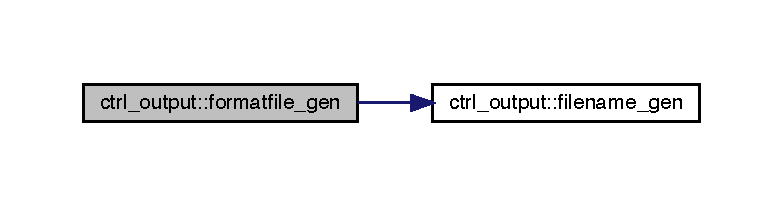
\includegraphics[width=350pt]{namespacectrl__output_a754f1fcb7692b22f531bcbd7fffd2634_cgraph}
\end{center}
\end{figure}
\mbox{\Hypertarget{namespacectrl__output_a7c804abccd932d50e4938262f22f586e}\label{namespacectrl__output_a7c804abccd932d50e4938262f22f586e}} 
\index{ctrl\+\_\+output@{ctrl\+\_\+output}!grid2mat@{grid2mat}}
\index{grid2mat@{grid2mat}!ctrl\+\_\+output@{ctrl\+\_\+output}}
\subsubsection{\texorpdfstring{grid2mat()}{grid2mat()}}
{\footnotesize\ttfamily subroutine ctrl\+\_\+output\+::grid2mat (\begin{DoxyParamCaption}\item[{integer, dimension(nrow$\ast$ncol)}]{seq\+Grid2\+Sort,  }\item[{integer, dimension(nrow$\ast$ncol)}]{seq\+Grid\+Sorted,  }\item[{integer, dimension(nrow,ncol)}]{mat\+Grid,  }\item[{integer}]{n\+Row,  }\item[{integer}]{n\+Col }\end{DoxyParamCaption})}



Definition at line 1213 of file S\+U\+E\+W\+S\+\_\+ctrl\+\_\+output.\+f95.

Here is the call graph for this function\+:\nopagebreak
\begin{figure}[H]
\begin{center}
\leavevmode
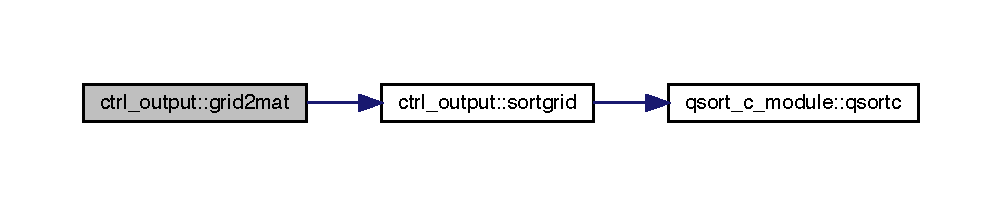
\includegraphics[width=350pt]{namespacectrl__output_a7c804abccd932d50e4938262f22f586e_cgraph}
\end{center}
\end{figure}
\mbox{\Hypertarget{namespacectrl__output_a06abc3039b8c610cb65b9cd42817d064}\label{namespacectrl__output_a06abc3039b8c610cb65b9cd42817d064}} 
\index{ctrl\+\_\+output@{ctrl\+\_\+output}!seq2mat@{seq2mat}}
\index{seq2mat@{seq2mat}!ctrl\+\_\+output@{ctrl\+\_\+output}}
\subsubsection{\texorpdfstring{seq2mat()}{seq2mat()}}
{\footnotesize\ttfamily subroutine ctrl\+\_\+output\+::seq2mat (\begin{DoxyParamCaption}\item[{real(kind(1d0)), dimension(nrow$\ast$ncol)}]{seq2\+Sort,  }\item[{real(kind(1d0)), dimension(nrow$\ast$ncol)}]{seq\+Sorted,  }\item[{real(kind(1d0)), dimension(nrow,ncol)}]{mat\+Grid,  }\item[{integer}]{n\+Row,  }\item[{integer}]{n\+Col }\end{DoxyParamCaption})}



Definition at line 1244 of file S\+U\+E\+W\+S\+\_\+ctrl\+\_\+output.\+f95.

Here is the call graph for this function\+:\nopagebreak
\begin{figure}[H]
\begin{center}
\leavevmode
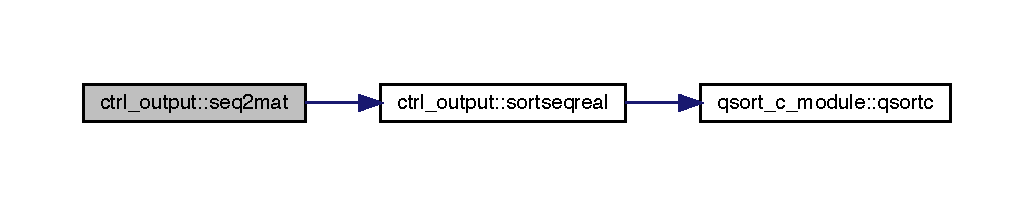
\includegraphics[width=350pt]{namespacectrl__output_a06abc3039b8c610cb65b9cd42817d064_cgraph}
\end{center}
\end{figure}
\mbox{\Hypertarget{namespacectrl__output_a1807dd1d886e5fd090461e140156758b}\label{namespacectrl__output_a1807dd1d886e5fd090461e140156758b}} 
\index{ctrl\+\_\+output@{ctrl\+\_\+output}!sortgrid@{sortgrid}}
\index{sortgrid@{sortgrid}!ctrl\+\_\+output@{ctrl\+\_\+output}}
\subsubsection{\texorpdfstring{sortgrid()}{sortgrid()}}
{\footnotesize\ttfamily subroutine ctrl\+\_\+output\+::sortgrid (\begin{DoxyParamCaption}\item[{integer, dimension(nrow$\ast$ncol), intent(in)}]{seq\+Grid2\+Sort,  }\item[{integer, dimension(nrow$\ast$ncol), intent(out)}]{seq\+Grid\+Sorted,  }\item[{integer}]{n\+Row,  }\item[{integer}]{n\+Col }\end{DoxyParamCaption})}



Definition at line 1271 of file S\+U\+E\+W\+S\+\_\+ctrl\+\_\+output.\+f95.

Here is the call graph for this function\+:\nopagebreak
\begin{figure}[H]
\begin{center}
\leavevmode
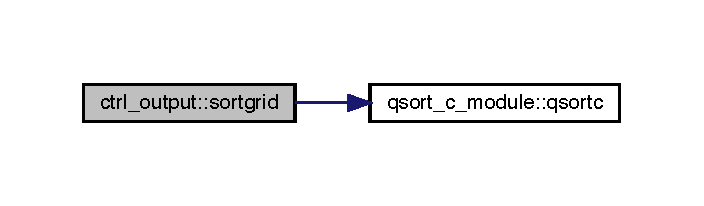
\includegraphics[width=338pt]{namespacectrl__output_a1807dd1d886e5fd090461e140156758b_cgraph}
\end{center}
\end{figure}
\mbox{\Hypertarget{namespacectrl__output_a093211a59ed2a27d1d853afc548146df}\label{namespacectrl__output_a093211a59ed2a27d1d853afc548146df}} 
\index{ctrl\+\_\+output@{ctrl\+\_\+output}!sortseqreal@{sortseqreal}}
\index{sortseqreal@{sortseqreal}!ctrl\+\_\+output@{ctrl\+\_\+output}}
\subsubsection{\texorpdfstring{sortseqreal()}{sortseqreal()}}
{\footnotesize\ttfamily subroutine ctrl\+\_\+output\+::sortseqreal (\begin{DoxyParamCaption}\item[{real(kind(1d0)), dimension(nrow$\ast$ncol), intent(in)}]{seq\+Real2\+Sort,  }\item[{real(kind(1d0)), dimension(nrow$\ast$ncol), intent(out)}]{seq\+Real\+Sorted,  }\item[{integer}]{n\+Row,  }\item[{integer}]{n\+Col }\end{DoxyParamCaption})}



Definition at line 1356 of file S\+U\+E\+W\+S\+\_\+ctrl\+\_\+output.\+f95.

Here is the call graph for this function\+:\nopagebreak
\begin{figure}[H]
\begin{center}
\leavevmode
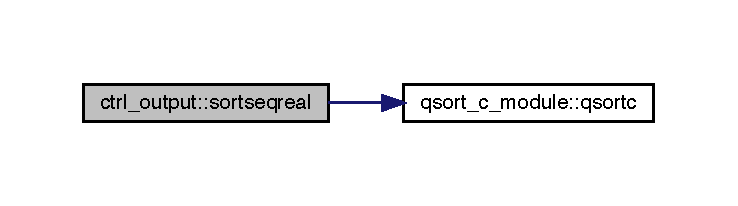
\includegraphics[width=350pt]{namespacectrl__output_a093211a59ed2a27d1d853afc548146df_cgraph}
\end{center}
\end{figure}
\mbox{\Hypertarget{namespacectrl__output_ae9a62c39f1b7598a639718dd95127977}\label{namespacectrl__output_ae9a62c39f1b7598a639718dd95127977}} 
\index{ctrl\+\_\+output@{ctrl\+\_\+output}!suews\+\_\+output\+\_\+agg@{suews\+\_\+output\+\_\+agg}}
\index{suews\+\_\+output\+\_\+agg@{suews\+\_\+output\+\_\+agg}!ctrl\+\_\+output@{ctrl\+\_\+output}}
\subsubsection{\texorpdfstring{suews\+\_\+output\+\_\+agg()}{suews\_output\_agg()}}
{\footnotesize\ttfamily subroutine ctrl\+\_\+output\+::suews\+\_\+output\+\_\+agg (\begin{DoxyParamCaption}\item[{real(kind(1d0)), dimension(\+:,\+:), intent(out), allocatable}]{data\+Out\+\_\+agg,  }\item[{real(kind(1d0)), dimension(\+:,\+:), intent(in)}]{data\+Out,  }\item[{type(\hyperlink{structctrl__output_1_1varattr}{varattr}), dimension(\+:), intent(in)}]{var\+List,  }\item[{integer, intent(in)}]{ir\+Max,  }\item[{integer, intent(in)}]{out\+Freq\+\_\+s }\end{DoxyParamCaption})}



Definition at line 648 of file S\+U\+E\+W\+S\+\_\+ctrl\+\_\+output.\+f95.

\mbox{\Hypertarget{namespacectrl__output_aa089b1e6d88c1556fb0d0f645face272}\label{namespacectrl__output_aa089b1e6d88c1556fb0d0f645face272}} 
\index{ctrl\+\_\+output@{ctrl\+\_\+output}!suews\+\_\+output\+\_\+init@{suews\+\_\+output\+\_\+init}}
\index{suews\+\_\+output\+\_\+init@{suews\+\_\+output\+\_\+init}!ctrl\+\_\+output@{ctrl\+\_\+output}}
\subsubsection{\texorpdfstring{suews\+\_\+output\+\_\+init()}{suews\_output\_init()}}
{\footnotesize\ttfamily subroutine ctrl\+\_\+output\+::suews\+\_\+output\+\_\+init (\begin{DoxyParamCaption}\item[{real(kind(1d0)), dimension(\+:,\+:), intent(in)}]{data\+Out,  }\item[{type(\hyperlink{structctrl__output_1_1varattr}{varattr}), dimension(\+:), intent(in)}]{var\+List,  }\item[{integer, intent(in)}]{Gridiv,  }\item[{integer, intent(in)}]{out\+Level }\end{DoxyParamCaption})}



Definition at line 475 of file S\+U\+E\+W\+S\+\_\+ctrl\+\_\+output.\+f95.

Here is the call graph for this function\+:\nopagebreak
\begin{figure}[H]
\begin{center}
\leavevmode
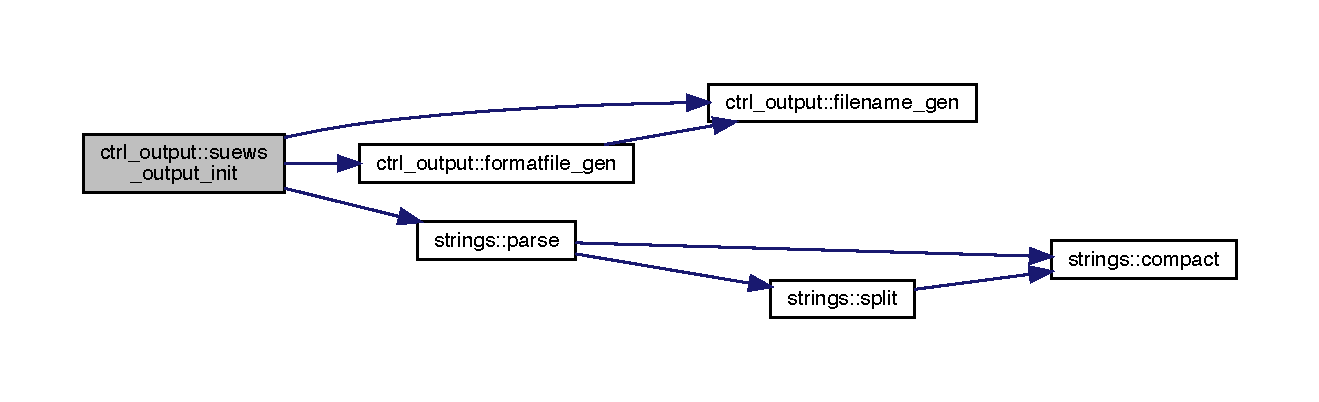
\includegraphics[width=350pt]{namespacectrl__output_aa089b1e6d88c1556fb0d0f645face272_cgraph}
\end{center}
\end{figure}
\mbox{\Hypertarget{namespacectrl__output_abe2b9152111665466982f35349bf24d8}\label{namespacectrl__output_abe2b9152111665466982f35349bf24d8}} 
\index{ctrl\+\_\+output@{ctrl\+\_\+output}!suews\+\_\+output\+\_\+nc@{suews\+\_\+output\+\_\+nc}}
\index{suews\+\_\+output\+\_\+nc@{suews\+\_\+output\+\_\+nc}!ctrl\+\_\+output@{ctrl\+\_\+output}}
\subsubsection{\texorpdfstring{suews\+\_\+output\+\_\+nc()}{suews\_output\_nc()}}
{\footnotesize\ttfamily subroutine ctrl\+\_\+output\+::suews\+\_\+output\+\_\+nc (\begin{DoxyParamCaption}\item[{integer, intent(in)}]{ir\+Max }\end{DoxyParamCaption})}



Definition at line 885 of file S\+U\+E\+W\+S\+\_\+ctrl\+\_\+output.\+f95.

Here is the call graph for this function\+:\nopagebreak
\begin{figure}[H]
\begin{center}
\leavevmode
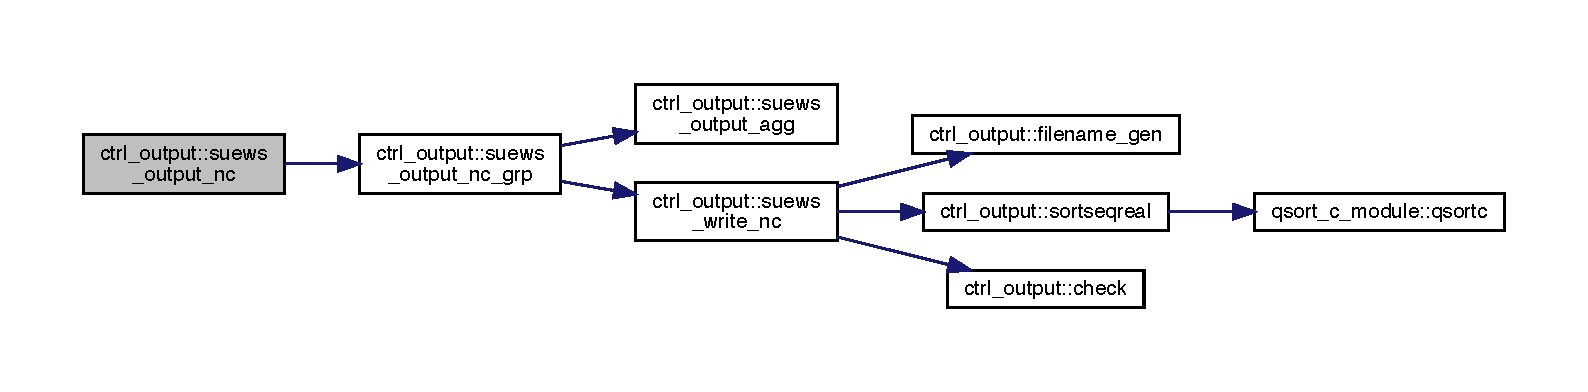
\includegraphics[width=350pt]{namespacectrl__output_abe2b9152111665466982f35349bf24d8_cgraph}
\end{center}
\end{figure}
\mbox{\Hypertarget{namespacectrl__output_a333bec5a308bd89762292b7f695bdb9b}\label{namespacectrl__output_a333bec5a308bd89762292b7f695bdb9b}} 
\index{ctrl\+\_\+output@{ctrl\+\_\+output}!suews\+\_\+output\+\_\+nc\+\_\+grp@{suews\+\_\+output\+\_\+nc\+\_\+grp}}
\index{suews\+\_\+output\+\_\+nc\+\_\+grp@{suews\+\_\+output\+\_\+nc\+\_\+grp}!ctrl\+\_\+output@{ctrl\+\_\+output}}
\subsubsection{\texorpdfstring{suews\+\_\+output\+\_\+nc\+\_\+grp()}{suews\_output\_nc\_grp()}}
{\footnotesize\ttfamily subroutine ctrl\+\_\+output\+::suews\+\_\+output\+\_\+nc\+\_\+grp (\begin{DoxyParamCaption}\item[{integer, intent(in)}]{ir\+Max,  }\item[{type(\hyperlink{structctrl__output_1_1varattr}{varattr}), dimension(\+:), intent(in)}]{var\+List,  }\item[{integer, intent(in)}]{out\+Level,  }\item[{integer, intent(in)}]{out\+Freq\+\_\+s }\end{DoxyParamCaption})}



Definition at line 959 of file S\+U\+E\+W\+S\+\_\+ctrl\+\_\+output.\+f95.

Here is the call graph for this function\+:\nopagebreak
\begin{figure}[H]
\begin{center}
\leavevmode
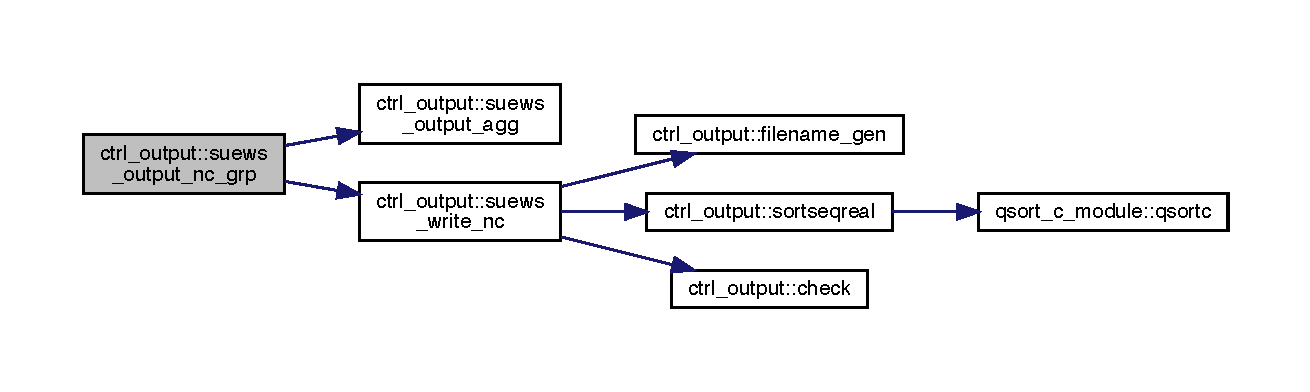
\includegraphics[width=350pt]{namespacectrl__output_a333bec5a308bd89762292b7f695bdb9b_cgraph}
\end{center}
\end{figure}
\mbox{\Hypertarget{namespacectrl__output_a33e3b788edad27be3211458c4388f8e5}\label{namespacectrl__output_a33e3b788edad27be3211458c4388f8e5}} 
\index{ctrl\+\_\+output@{ctrl\+\_\+output}!suews\+\_\+output\+\_\+txt@{suews\+\_\+output\+\_\+txt}}
\index{suews\+\_\+output\+\_\+txt@{suews\+\_\+output\+\_\+txt}!ctrl\+\_\+output@{ctrl\+\_\+output}}
\subsubsection{\texorpdfstring{suews\+\_\+output\+\_\+txt()}{suews\_output\_txt()}}
{\footnotesize\ttfamily subroutine ctrl\+\_\+output\+::suews\+\_\+output\+\_\+txt (\begin{DoxyParamCaption}\item[{integer, intent(in)}]{iv,  }\item[{integer, intent(in)}]{ir\+Max,  }\item[{integer, intent(in)}]{Gridiv }\end{DoxyParamCaption})}



Definition at line 346 of file S\+U\+E\+W\+S\+\_\+ctrl\+\_\+output.\+f95.

Here is the call graph for this function\+:\nopagebreak
\begin{figure}[H]
\begin{center}
\leavevmode
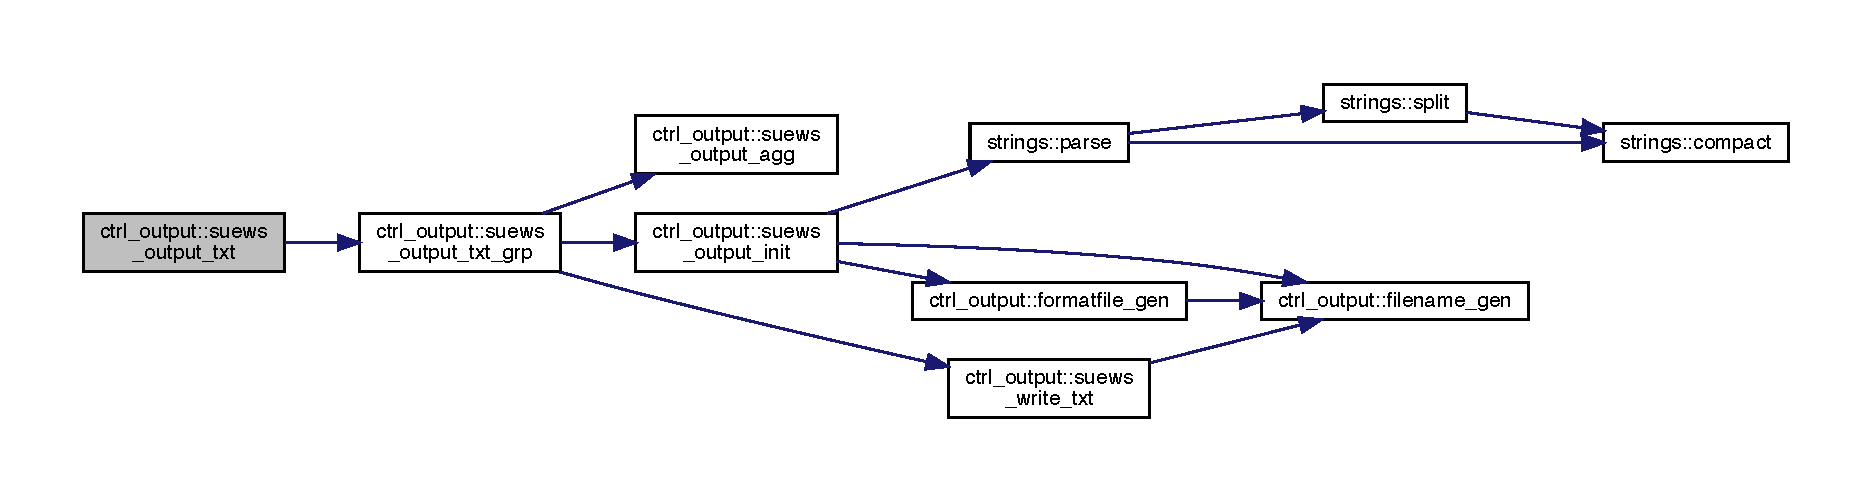
\includegraphics[width=350pt]{namespacectrl__output_a33e3b788edad27be3211458c4388f8e5_cgraph}
\end{center}
\end{figure}
\mbox{\Hypertarget{namespacectrl__output_ac3541cbdb88f9028bc3592ee65b64980}\label{namespacectrl__output_ac3541cbdb88f9028bc3592ee65b64980}} 
\index{ctrl\+\_\+output@{ctrl\+\_\+output}!suews\+\_\+output\+\_\+txt\+\_\+grp@{suews\+\_\+output\+\_\+txt\+\_\+grp}}
\index{suews\+\_\+output\+\_\+txt\+\_\+grp@{suews\+\_\+output\+\_\+txt\+\_\+grp}!ctrl\+\_\+output@{ctrl\+\_\+output}}
\subsubsection{\texorpdfstring{suews\+\_\+output\+\_\+txt\+\_\+grp()}{suews\_output\_txt\_grp()}}
{\footnotesize\ttfamily subroutine ctrl\+\_\+output\+::suews\+\_\+output\+\_\+txt\+\_\+grp (\begin{DoxyParamCaption}\item[{integer, intent(in)}]{iv,  }\item[{integer, intent(in)}]{ir\+Max,  }\item[{type(\hyperlink{structctrl__output_1_1varattr}{varattr}), dimension(\+:), intent(in)}]{var\+List,  }\item[{integer, intent(in)}]{Gridiv,  }\item[{integer, intent(in)}]{out\+Level,  }\item[{integer, intent(in)}]{out\+Freq\+\_\+s }\end{DoxyParamCaption})}



Definition at line 426 of file S\+U\+E\+W\+S\+\_\+ctrl\+\_\+output.\+f95.

Here is the call graph for this function\+:\nopagebreak
\begin{figure}[H]
\begin{center}
\leavevmode
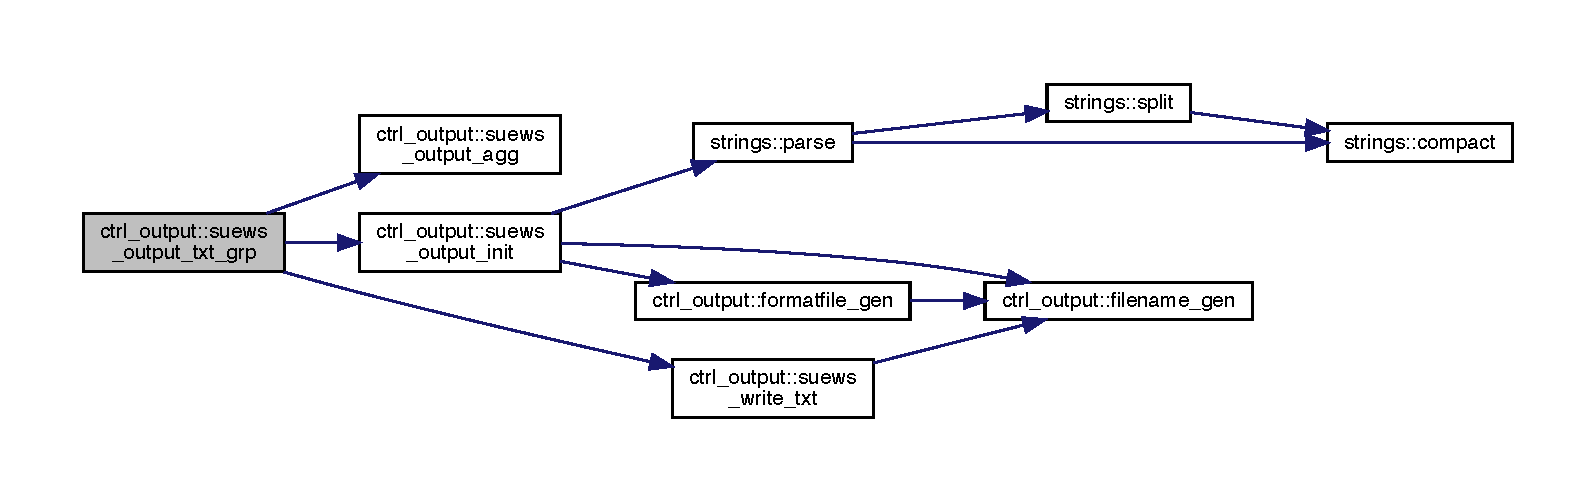
\includegraphics[width=350pt]{namespacectrl__output_ac3541cbdb88f9028bc3592ee65b64980_cgraph}
\end{center}
\end{figure}
\mbox{\Hypertarget{namespacectrl__output_a34f8d939c96cb60cdf1f9739e1ea4672}\label{namespacectrl__output_a34f8d939c96cb60cdf1f9739e1ea4672}} 
\index{ctrl\+\_\+output@{ctrl\+\_\+output}!suews\+\_\+write\+\_\+nc@{suews\+\_\+write\+\_\+nc}}
\index{suews\+\_\+write\+\_\+nc@{suews\+\_\+write\+\_\+nc}!ctrl\+\_\+output@{ctrl\+\_\+output}}
\subsubsection{\texorpdfstring{suews\+\_\+write\+\_\+nc()}{suews\_write\_nc()}}
{\footnotesize\ttfamily subroutine ctrl\+\_\+output\+::suews\+\_\+write\+\_\+nc (\begin{DoxyParamCaption}\item[{real(kind(1d0)), dimension(\+:,\+:,\+:), intent(in)}]{data\+Out,  }\item[{type(\hyperlink{structctrl__output_1_1varattr}{varattr}), dimension(\+:), intent(in)}]{var\+List,  }\item[{integer, intent(in)}]{out\+Level }\end{DoxyParamCaption})}



Definition at line 1006 of file S\+U\+E\+W\+S\+\_\+ctrl\+\_\+output.\+f95.

Here is the call graph for this function\+:\nopagebreak
\begin{figure}[H]
\begin{center}
\leavevmode
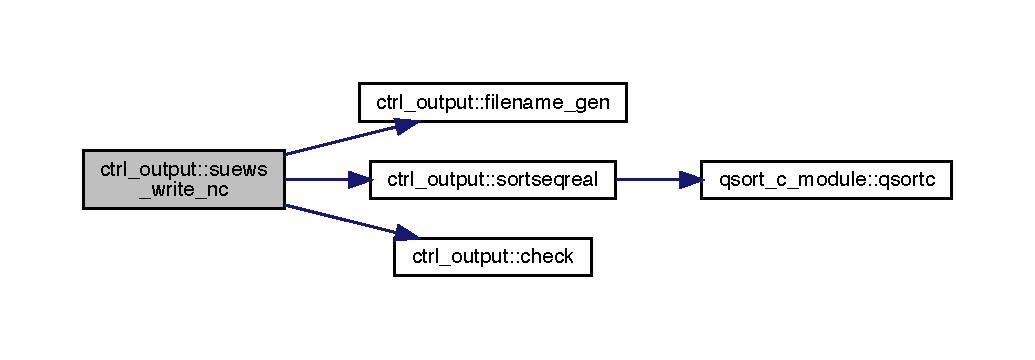
\includegraphics[width=350pt]{namespacectrl__output_a34f8d939c96cb60cdf1f9739e1ea4672_cgraph}
\end{center}
\end{figure}
\mbox{\Hypertarget{namespacectrl__output_a84e30d3564e406535ea078c470a62668}\label{namespacectrl__output_a84e30d3564e406535ea078c470a62668}} 
\index{ctrl\+\_\+output@{ctrl\+\_\+output}!suews\+\_\+write\+\_\+txt@{suews\+\_\+write\+\_\+txt}}
\index{suews\+\_\+write\+\_\+txt@{suews\+\_\+write\+\_\+txt}!ctrl\+\_\+output@{ctrl\+\_\+output}}
\subsubsection{\texorpdfstring{suews\+\_\+write\+\_\+txt()}{suews\_write\_txt()}}
{\footnotesize\ttfamily subroutine ctrl\+\_\+output\+::suews\+\_\+write\+\_\+txt (\begin{DoxyParamCaption}\item[{real(kind(1d0)), dimension(\+:,\+:), intent(in)}]{data\+Out,  }\item[{type(\hyperlink{structctrl__output_1_1varattr}{varattr}), dimension(\+:), intent(in)}]{var\+List,  }\item[{integer, intent(in)}]{Gridiv,  }\item[{integer, intent(in)}]{out\+Level }\end{DoxyParamCaption})}



Definition at line 697 of file S\+U\+E\+W\+S\+\_\+ctrl\+\_\+output.\+f95.

Here is the call graph for this function\+:\nopagebreak
\begin{figure}[H]
\begin{center}
\leavevmode
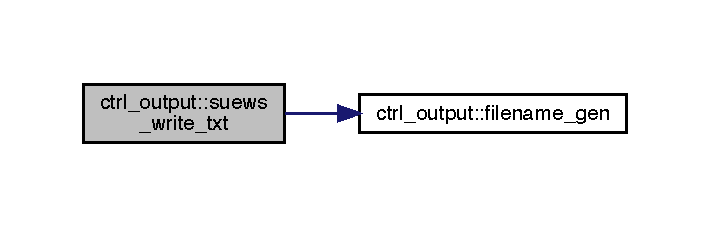
\includegraphics[width=341pt]{namespacectrl__output_a84e30d3564e406535ea078c470a62668_cgraph}
\end{center}
\end{figure}


\subsection{Variable Documentation}
\mbox{\Hypertarget{namespacectrl__output_a51a0e846694f677a954a439b2d0069ce}\label{namespacectrl__output_a51a0e846694f677a954a439b2d0069ce}} 
\index{ctrl\+\_\+output@{ctrl\+\_\+output}!aa@{aa}}
\index{aa@{aa}!ctrl\+\_\+output@{ctrl\+\_\+output}}
\subsubsection{\texorpdfstring{aa}{aa}}
{\footnotesize\ttfamily character(len= 1), parameter ctrl\+\_\+output\+::aa = \textquotesingle{}1\textquotesingle{}}



Definition at line 49 of file S\+U\+E\+W\+S\+\_\+ctrl\+\_\+output.\+f95.

\mbox{\Hypertarget{namespacectrl__output_a0cab13c6b1b664657d53f54bcaaf0b93}\label{namespacectrl__output_a0cab13c6b1b664657d53f54bcaaf0b93}} 
\index{ctrl\+\_\+output@{ctrl\+\_\+output}!al@{al}}
\index{al@{al}!ctrl\+\_\+output@{ctrl\+\_\+output}}
\subsubsection{\texorpdfstring{al}{al}}
{\footnotesize\ttfamily character(len= 1), parameter ctrl\+\_\+output\+::al = \textquotesingle{}3\textquotesingle{}}



Definition at line 49 of file S\+U\+E\+W\+S\+\_\+ctrl\+\_\+output.\+f95.

\mbox{\Hypertarget{namespacectrl__output_a27bc52c96e692d0dbe7f6f73a3aea7e7}\label{namespacectrl__output_a27bc52c96e692d0dbe7f6f73a3aea7e7}} 
\index{ctrl\+\_\+output@{ctrl\+\_\+output}!as@{as}}
\index{as@{as}!ctrl\+\_\+output@{ctrl\+\_\+output}}
\subsubsection{\texorpdfstring{as}{as}}
{\footnotesize\ttfamily character(len= 1), parameter ctrl\+\_\+output\+::as = \textquotesingle{}2\textquotesingle{}}



Definition at line 49 of file S\+U\+E\+W\+S\+\_\+ctrl\+\_\+output.\+f95.

\mbox{\Hypertarget{namespacectrl__output_a18321fc13d7efb9b006ac70cece45909}\label{namespacectrl__output_a18321fc13d7efb9b006ac70cece45909}} 
\index{ctrl\+\_\+output@{ctrl\+\_\+output}!at@{at}}
\index{at@{at}!ctrl\+\_\+output@{ctrl\+\_\+output}}
\subsubsection{\texorpdfstring{at}{at}}
{\footnotesize\ttfamily character(len= 1), parameter ctrl\+\_\+output\+::at = \textquotesingle{}0\textquotesingle{}}



Definition at line 49 of file S\+U\+E\+W\+S\+\_\+ctrl\+\_\+output.\+f95.

\mbox{\Hypertarget{namespacectrl__output_a8653fec4faca8b39551da13d93a3f223}\label{namespacectrl__output_a8653fec4faca8b39551da13d93a3f223}} 
\index{ctrl\+\_\+output@{ctrl\+\_\+output}!f104@{f104}}
\index{f104@{f104}!ctrl\+\_\+output@{ctrl\+\_\+output}}
\subsubsection{\texorpdfstring{f104}{f104}}
{\footnotesize\ttfamily character(len=10), parameter ctrl\+\_\+output\+::f104 = \textquotesingle{}(f10.\+4,1\+X)\textquotesingle{}}



Definition at line 40 of file S\+U\+E\+W\+S\+\_\+ctrl\+\_\+output.\+f95.

\mbox{\Hypertarget{namespacectrl__output_a191786067cffb2dc5dcfcafb12b2ead6}\label{namespacectrl__output_a191786067cffb2dc5dcfcafb12b2ead6}} 
\index{ctrl\+\_\+output@{ctrl\+\_\+output}!f106@{f106}}
\index{f106@{f106}!ctrl\+\_\+output@{ctrl\+\_\+output}}
\subsubsection{\texorpdfstring{f106}{f106}}
{\footnotesize\ttfamily character(len=10), parameter ctrl\+\_\+output\+::f106 = \textquotesingle{}(f10.\+6,1\+X)\textquotesingle{}}



Definition at line 40 of file S\+U\+E\+W\+S\+\_\+ctrl\+\_\+output.\+f95.

\mbox{\Hypertarget{namespacectrl__output_a524b25246e690cfbc8f75fe72938fb06}\label{namespacectrl__output_a524b25246e690cfbc8f75fe72938fb06}} 
\index{ctrl\+\_\+output@{ctrl\+\_\+output}!f146@{f146}}
\index{f146@{f146}!ctrl\+\_\+output@{ctrl\+\_\+output}}
\subsubsection{\texorpdfstring{f146}{f146}}
{\footnotesize\ttfamily character(len=10), parameter ctrl\+\_\+output\+::f146 = \textquotesingle{}(f14.\+6,1\+X)\textquotesingle{}}



Definition at line 40 of file S\+U\+E\+W\+S\+\_\+ctrl\+\_\+output.\+f95.

\mbox{\Hypertarget{namespacectrl__output_a11f0b66275fc65047967ff8b2050ad25}\label{namespacectrl__output_a11f0b66275fc65047967ff8b2050ad25}} 
\index{ctrl\+\_\+output@{ctrl\+\_\+output}!f94@{f94}}
\index{f94@{f94}!ctrl\+\_\+output@{ctrl\+\_\+output}}
\subsubsection{\texorpdfstring{f94}{f94}}
{\footnotesize\ttfamily character(len=10), parameter ctrl\+\_\+output\+::f94 = \textquotesingle{}(f09.\+4,1\+X)\textquotesingle{}}



Definition at line 40 of file S\+U\+E\+W\+S\+\_\+ctrl\+\_\+output.\+f95.

\mbox{\Hypertarget{namespacectrl__output_aa27783daf4b75a43cae98a60ce884744}\label{namespacectrl__output_aa27783daf4b75a43cae98a60ce884744}} 
\index{ctrl\+\_\+output@{ctrl\+\_\+output}!fd@{fd}}
\index{fd@{fd}!ctrl\+\_\+output@{ctrl\+\_\+output}}
\subsubsection{\texorpdfstring{fd}{fd}}
{\footnotesize\ttfamily character(len=10), parameter ctrl\+\_\+output\+::fd = \textquotesingle{}(f08.\+4,1\+X)\textquotesingle{}}



Definition at line 40 of file S\+U\+E\+W\+S\+\_\+ctrl\+\_\+output.\+f95.

\mbox{\Hypertarget{namespacectrl__output_a2b5a74f7a69e74fed45533d69b5fcf81}\label{namespacectrl__output_a2b5a74f7a69e74fed45533d69b5fcf81}} 
\index{ctrl\+\_\+output@{ctrl\+\_\+output}!ft@{ft}}
\index{ft@{ft}!ctrl\+\_\+output@{ctrl\+\_\+output}}
\subsubsection{\texorpdfstring{ft}{ft}}
{\footnotesize\ttfamily character(len=10), parameter ctrl\+\_\+output\+::ft = \textquotesingle{}(i0004,1\+X)\textquotesingle{}}



Definition at line 40 of file S\+U\+E\+W\+S\+\_\+ctrl\+\_\+output.\+f95.

\mbox{\Hypertarget{namespacectrl__output_a250aeaca42269ac3898762523ec86e22}\label{namespacectrl__output_a250aeaca42269ac3898762523ec86e22}} 
\index{ctrl\+\_\+output@{ctrl\+\_\+output}!fy@{fy}}
\index{fy@{fy}!ctrl\+\_\+output@{ctrl\+\_\+output}}
\subsubsection{\texorpdfstring{fy}{fy}}
{\footnotesize\ttfamily character(len=10), parameter ctrl\+\_\+output\+::fy = \textquotesingle{}(i0004,1\+X)\textquotesingle{}}



Definition at line 40 of file S\+U\+E\+W\+S\+\_\+ctrl\+\_\+output.\+f95.

\mbox{\Hypertarget{namespacectrl__output_a0e436b9299ebba225dbe6a2f4eff2eed}\label{namespacectrl__output_a0e436b9299ebba225dbe6a2f4eff2eed}} 
\index{ctrl\+\_\+output@{ctrl\+\_\+output}!i@{i}}
\index{i@{i}!ctrl\+\_\+output@{ctrl\+\_\+output}}
\subsubsection{\texorpdfstring{i}{i}}
{\footnotesize\ttfamily integer ctrl\+\_\+output\+::i}



Definition at line 38 of file S\+U\+E\+W\+S\+\_\+ctrl\+\_\+output.\+f95.

\mbox{\Hypertarget{namespacectrl__output_a4c25bfab41d6433c78b76c0a0d9c03b8}\label{namespacectrl__output_a4c25bfab41d6433c78b76c0a0d9c03b8}} 
\index{ctrl\+\_\+output@{ctrl\+\_\+output}!itext@{itext}}
\index{itext@{itext}!ctrl\+\_\+output@{ctrl\+\_\+output}}
\subsubsection{\texorpdfstring{itext}{itext}}
{\footnotesize\ttfamily character(len= 3) ctrl\+\_\+output\+::itext}



Definition at line 55 of file S\+U\+E\+W\+S\+\_\+ctrl\+\_\+output.\+f95.

\mbox{\Hypertarget{namespacectrl__output_abf54926f3da30aea81f0d2ddfc9f4649}\label{namespacectrl__output_abf54926f3da30aea81f0d2ddfc9f4649}} 
\index{ctrl\+\_\+output@{ctrl\+\_\+output}!varlist@{varlist}}
\index{varlist@{varlist}!ctrl\+\_\+output@{ctrl\+\_\+output}}
\subsubsection{\texorpdfstring{varlist}{varlist}}
{\footnotesize\ttfamily type(\hyperlink{structctrl__output_1_1varattr}{varattr}), dimension(300) ctrl\+\_\+output\+::varlist}



Definition at line 69 of file S\+U\+E\+W\+S\+\_\+ctrl\+\_\+output.\+f95.


\hypertarget{namespacedata__in}{}\section{data\+\_\+in Module Reference}
\label{namespacedata__in}\index{data\+\_\+in@{data\+\_\+in}}
\subsection*{Variables}
\begin{DoxyCompactItemize}
\item 
character(len=90) \hyperlink{namespacedata__in_a7dd6ee68e2bde1c81c0ed1b6a6e9061b}{progname} =\textquotesingle{}S\+U\+E\+WS V2017a\textquotesingle{}
\begin{DoxyCompactList}\small\item\em $<$$<$$<$$<$$<$$<$$<$$<$$<$$<$$<$$<$$<$$<$$<$$<$$<$ \end{DoxyCompactList}\item 
character(len=20) \hyperlink{namespacedata__in_a7f8949b7ebf799e7223eae9fd01a7749}{filecode}
\item 
character(len=150) \hyperlink{namespacedata__in_a67f60bb1f8edd3c6be5380ab655fe7f1}{fileinputpath}
\item 
character(len=150) \hyperlink{namespacedata__in_a62ca2dcc9ca96142df62a94056f96391}{fileoutputpath}
\item 
character(len=150) \hyperlink{namespacedata__in_ac2b450671084fe099a448b9041377812}{fileout}
\item 
character(len=150) \hyperlink{namespacedata__in_a06dcdca28402576db115b411e6a1f090}{filechoices}
\item 
character(len=150) \hyperlink{namespacedata__in_a47dbe76dba82734e5409c2ee5cc0a1d8}{filemet}
\item 
character(len=150) \hyperlink{namespacedata__in_aa954c0fba57d9145cc0c6336009d06bf}{fileorigmet}
\item 
character(len=150) \hyperlink{namespacedata__in_a9cc7b5d1b7fbb824210f4f81d0498bd0}{fileorigestm}
\item 
character(len=150) \hyperlink{namespacedata__in_ad0d0971b802f95d1a4fcc057771aee6b}{filedscdmet}
\item 
character(len=150) \hyperlink{namespacedata__in_aae47ad70ed5c4116cec7838aaaaa302a}{filedscdestm}
\item 
character(len=150) \hyperlink{namespacedata__in_a46e1032d2b5b787e36c022a180204a49}{filedaily}
\item 
character(len=150) \hyperlink{namespacedata__in_a01c2281eb3d97cb6f8fbd7b5e03d33e2}{fileestmts}
\item 
character(len=150) \hyperlink{namespacedata__in_a08b0a2fffc34dcaefd3ef81483777e4e}{solweigpoiout}
\item 
character(len=150) \hyperlink{namespacedata__in_ac7dd014c6f349ee2b4c385f79348fff4}{blout}
\item 
character(len=150) \hyperlink{namespacedata__in_a0bc6e84d091c3af529338729ef26182a}{fileout\+\_\+tt}
\item 
character(len=150) \hyperlink{namespacedata__in_ab3963c227716bf7ca52ecd4fcc7a8e67}{estmout\+\_\+tt}
\item 
integer \hyperlink{namespacedata__in_a964397f0f83d198e4f674a85b7be941a}{skipheadersiteinfo} = 2
\item 
integer \hyperlink{namespacedata__in_aea829593453d36d348e367b3238f63ea}{skipheadermet} = 1
\item 
integer \hyperlink{namespacedata__in_a2d5ce0a221d7ee5c42ab2bdb3bf06a8b}{anthropheatmethod}
\item 
integer \hyperlink{namespacedata__in_a6bf8149cf01d75c9bfb8b7aa575b98c3}{anthropco2method}
\item 
integer \hyperlink{namespacedata__in_a0baf7befb79fdeb3a9b4a5107f64d25c}{cbluse}
\item 
integer \hyperlink{namespacedata__in_a1de5c53755db8632301d4d1897f3ee8f}{multiplemetfiles}
\item 
integer \hyperlink{namespacedata__in_ab28ac9ca6b8ed723ce3e74496158c5c8}{multipleinitfiles}
\item 
integer \hyperlink{namespacedata__in_ad49de355a2aafe1ffbc40d2e91a12d87}{multipleestmfiles}
\item 
integer \hyperlink{namespacedata__in_a66e75b7142f8d93aecf0a9c94a8a25d9}{keeptstepfilesin}
\item 
integer \hyperlink{namespacedata__in_ab9a0f114993684cd73bedea082abe184}{keeptstepfilesout}
\item 
integer \hyperlink{namespacedata__in_a0dfb19ee9c3d77d6a086f17b231d65b8}{resolutionfilesin}
\item 
integer \hyperlink{namespacedata__in_a6ea370f15cdb7fab545340173792072a}{resolutionfilesout}
\item 
integer \hyperlink{namespacedata__in_a1babc329d678c128938354d4c21505b9}{resolutionfilesinestm}
\item 
integer \hyperlink{namespacedata__in_a902aee6a424a884da4775e7a40782896}{writeoutoption}
\item 
integer \hyperlink{namespacedata__in_a0b433ad2361360f657c537b128e4a5f7}{netradiationmethod}
\item 
integer \hyperlink{namespacedata__in_a27bd8e1db530bad815c128979003c184}{ohmincqf}
\item 
integer \hyperlink{namespacedata__in_aba572e9ad5577e14bcd393849b1fcdf3}{storageheatmethod}
\item 
integer \hyperlink{namespacedata__in_a43b72c0ea9c40a969cac5f758c240815}{snowuse}
\item 
integer \hyperlink{namespacedata__in_a6cc0dbee756c4ddc20f395bd37f7ad8f}{solweiguse}
\item 
integer \hyperlink{namespacedata__in_a306f10a44e3e8097152fc6a9c0403f6b}{smdmethod}
\item 
integer \hyperlink{namespacedata__in_ab3b82014d0bd4e04ce70642a274dd0dc}{waterusemethod}
\item 
integer \hyperlink{namespacedata__in_ae0baee62dbc6ad6a70c51f5eb1c1882b}{roughlenmommethod}
\item 
integer \hyperlink{namespacedata__in_acdfe353290d799264bab6281a87a1fa7}{disaggmethod}
\item 
integer \hyperlink{namespacedata__in_a672fba472da09ab270c02ec3e92ff9a3}{disaggmethodestm}
\item 
integer \hyperlink{namespacedata__in_ae443b92cf02ecc9331aa9f83b2101f90}{raindisaggmethod}
\item 
integer \hyperlink{namespacedata__in_ac8669fa345dd942fb34ee438634579a4}{rainamongn}
\item 
integer \hyperlink{namespacedata__in_ad7a96eb31a956b650073fc7135d307cd}{kdownzen}
\item 
integer \hyperlink{namespacedata__in_a70af1f33c9424336cb42b8c11bfdf51f}{suppresswarnings}
\item 
integer \hyperlink{namespacedata__in_aa277445969a4533d0db8452d45164762}{diagnose}
\item 
integer \hyperlink{namespacedata__in_a4083646fdfcd997307f15597aa4ec662}{diagnosedisagg}
\item 
integer \hyperlink{namespacedata__in_a8c3e4136805b6c64af2129539988ed09}{ncmode}
\item 
integer \hyperlink{namespacedata__in_ab7209967962bb333a35a29bb6a24eb36}{nrow}
\item 
integer \hyperlink{namespacedata__in_abcffd65e274aa3e20c73561543853e19}{ncol}
\item 
integer \hyperlink{namespacedata__in_ae4cd527d8942c93e41e59584292f2d9c}{diagnosedisaggestm}
\item 
integer \hyperlink{namespacedata__in_a2d6b128b5a2c8b851ee4fdd38204a18f}{diagqn}
\item 
integer \hyperlink{namespacedata__in_a2202e62dbdf6e4d935d472a09af97460}{diagqs}
\item 
integer, dimension(5) \hyperlink{namespacedata__in_a418fc51e58d7116a1764af37aba7b65f}{multrainamongn}
\item 
real(kind(1d0)), dimension(5) \hyperlink{namespacedata__in_a3473c34f53886b8fc852e23b09fc2add}{multrainamongnupperi}
\item 
integer \hyperlink{namespacedata__in_a95db274f3821ba4b3b2799481c2484f7}{albedochoice}
\item 
integer \hyperlink{namespacedata__in_a4abd9462bcbb39b3cab15d64ebe71995}{inputmetformat}
\item 
integer \hyperlink{namespacedata__in_a71e2da70dfd1593a6a4770f164bcc146}{ity}
\item 
integer \hyperlink{namespacedata__in_a3c3027e7975cd18122a58ae965ee0f86}{laicalcyes}
\item 
integer \hyperlink{namespacedata__in_adf35232d8407e784ed41dc8f09ffe171}{writedailystate}
\item 
integer \hyperlink{namespacedata__in_a7ee5c5c530300f6627f86b6cbde2d5b9}{ldown\+\_\+option}
\item 
integer \hyperlink{namespacedata__in_ad453037bad2cda84e61ec000bdd004aa}{lfnout}
\item 
integer \hyperlink{namespacedata__in_a0189adce2d060aee708a9216b5c771e2}{lfnoutc}
\item 
integer \hyperlink{namespacedata__in_a3b953424146f8076e9fec820cd6f31d2}{lfnold}
\item 
integer \hyperlink{namespacedata__in_afeae0c4bf24c4eea3af4a7fded472b26}{outputformats}
\item 
real(kind(1d0)) \hyperlink{namespacedata__in_ae7c74e8cbd3c208e00306eafe50a98c0}{timezone}
\item 
real(kind(1d0)) \hyperlink{namespacedata__in_a711f2f13bee1efd47bef091504e3621d}{ah\+\_\+min}
\item 
real(kind(1d0)) \hyperlink{namespacedata__in_ac10bf0a69520b391a81ee64742a4f6fd}{ah\+\_\+slope}
\item 
real(kind(1d0)) \hyperlink{namespacedata__in_a6ecf207ff2ecfcb35e223ad4e761ff9b}{alpha\+\_\+qhqe}
\item 
real(kind(1d0)) \hyperlink{namespacedata__in_a1f542f63d48efee0cd1e356f9f3ea1cf}{alt}
\item 
real(kind(1d0)) \hyperlink{namespacedata__in_abf271c3057b02dd9183e4442954c9577}{avdens}
\item 
real(kind(1d0)) \hyperlink{namespacedata__in_a8ac4d9de71d52d8c39e04c59635a5e3c}{avkdn}
\item 
real(kind(1d0)) \hyperlink{namespacedata__in_a2c6cba95e27ebb1dcb673c457b66325d}{avrh}
\item 
real(kind(1d0)) \hyperlink{namespacedata__in_ab6a63bf1eb3d5838645b22b8f26bc97c}{avts}
\item 
real(kind(1d0)) \hyperlink{namespacedata__in_abc95201410a9b25f8d1d2d5a063302c3}{avu1}
\item 
real(kind(1d0)) \hyperlink{namespacedata__in_ad753c5f26f6cfaac607edf93d4c2dd1d}{avu10\+\_\+ms}
\item 
real(kind(1d0)) \hyperlink{namespacedata__in_a0abb9aefbb8c1dc5ac6ff2f770da7faa}{azimuth}
\item 
real(kind(1d0)) \hyperlink{namespacedata__in_a1e8b73a7f5e115a447c6d8317490a479}{basethdd}
\item 
real(kind(1d0)) \hyperlink{namespacedata__in_a181898a3db2411958a2a0f484e50a9f1}{buildenergyuse}
\item 
real(kind(1d0)) \hyperlink{namespacedata__in_a737780f5cf53c9f2d3048bbfface32cd}{e\+\_\+mod}
\item 
real(kind(1d0)) \hyperlink{namespacedata__in_a262cd82bafaff209c3bca1c3b368931b}{emis\+\_\+snow}
\item 
real(kind(1d0)) \hyperlink{namespacedata__in_a8bc526d8d9a75c1ecef04817aac48046}{fc}
\item 
real(kind(1d0)) \hyperlink{namespacedata__in_ad77982daffd6bf19ea51d6635d9d2009}{fc\+\_\+anthro}
\item 
real(kind(1d0)) \hyperlink{namespacedata__in_a446b6dc73d9c2e2518917361d9b526b3}{fc\+\_\+biogen}
\item 
real(kind(1d0)) \hyperlink{namespacedata__in_a39642f3fc927b3a4394dda8fef2c193b}{fc\+\_\+photo}
\item 
real(kind(1d0)) \hyperlink{namespacedata__in_a5d6aae5bf11940a5ff7437dfec30cd4f}{fc\+\_\+respi}
\item 
real(kind(1d0)) \hyperlink{namespacedata__in_a8676790950975f07daf8d24b503ef952}{fc\+\_\+metab}
\item 
real(kind(1d0)) \hyperlink{namespacedata__in_a9fcca4951f8282ad10df290f8a025387}{fc\+\_\+traff}
\item 
real(kind(1d0)) \hyperlink{namespacedata__in_a3c13cce56632f598e61b00bccdc94e4a}{fc\+\_\+build}
\item 
real(kind(1d0)) \hyperlink{namespacedata__in_a8afa15b03c067e57c570544bd5562ac1}{fcld}
\item 
real(kind(1d0)) \hyperlink{namespacedata__in_a03109ad2e583af2eb4b59e2e95758a72}{fcld\+\_\+obs}
\item 
real(kind(1d0)) \hyperlink{namespacedata__in_aaa77ae828595f5b1e1bec4237020dfbc}{h\+\_\+mod}
\item 
real(kind(1d0)) \hyperlink{namespacedata__in_ab31fbd3fd9d4036fa930706c4de36397}{kclear}
\item 
real(kind(1d0)) \hyperlink{namespacedata__in_ab7baf80fc15ebb7a7b739d064226a548}{kdiff}
\item 
real(kind(1d0)) \hyperlink{namespacedata__in_a4e6bf95c9d5bb3ea152dc358ac818008}{kdir}
\item 
real(kind(1d0)) \hyperlink{namespacedata__in_a5d9f4f79563d2e000333219a4d2f4c99}{kup}
\item 
real(kind(1d0)) \hyperlink{namespacedata__in_af9683d39e50e85ff167afd46236c7643}{lai\+\_\+obs}
\item 
real(kind(1d0)) \hyperlink{namespacedata__in_a364ff1ce2a4c78ea431e4dacbd66d6b4}{lat}
\item 
real(kind(1d0)) \hyperlink{namespacedata__in_a7be43e97ab4efa32b57c8f6b6b5949b7}{ldown}
\item 
real(kind(1d0)) \hyperlink{namespacedata__in_ad5a6e580db1d91b3cbb617a2bbee8d93}{ldown\+\_\+obs}
\item 
real(kind(1d0)) \hyperlink{namespacedata__in_a3604b533bd06593307e185fbbee27efb}{lng}
\item 
real(kind(1d0)) \hyperlink{namespacedata__in_a5a2c23ecc11fe337a954cca86be6e0ce}{lup}
\item 
real(kind(1d0)) \hyperlink{namespacedata__in_a6121773c8a8acb40d4c9501422264e15}{numcapita}
\item 
real(kind(1d0)) \hyperlink{namespacedata__in_a444b978c1a82b3eac7148ef35e9769c9}{popdensdaytime}
\item 
real(kind(1d0)) \hyperlink{namespacedata__in_a6b29a851fa3dca9d854a9078a37ad349}{popdensnighttime}
\item 
real(kind(1d0)) \hyperlink{namespacedata__in_affc86dfcf91974ff6d1768ff3b4406c3}{precip}
\item 
real(kind(1d0)) \hyperlink{namespacedata__in_aa3e790835200b911e51eba62d37a0c43}{precip\+\_\+hr}
\item 
real(kind(1d0)) \hyperlink{namespacedata__in_a03eea39f7275fe19868636524b857b6d}{press\+\_\+hpa}
\item 
real(kind(1d0)) \hyperlink{namespacedata__in_a63dc6d1a7d5f10b5c3ebd45aaffb7150}{pres\+\_\+kpa}
\item 
real(kind(1d0)) \hyperlink{namespacedata__in_a56c3960c55d29dadfd4d6be5ec53cc3c}{q2\+\_\+gkg}
\item 
real(kind(1d0)) \hyperlink{namespacedata__in_a15dff170cc3ed5a26f5b095eebf80392}{qe}
\item 
real(kind(1d0)) \hyperlink{namespacedata__in_a89bbf8e5d0059c1005799182e4f5f703}{qe\+\_\+obs}
\item 
real(kind(1d0)) \hyperlink{namespacedata__in_a13eb3e18ed56b78668ba6c47d11ba155}{qf}
\item 
real(kind(1d0)) \hyperlink{namespacedata__in_a3bdf6ad52d92cd85f212cea607807601}{qf\+\_\+sahp}
\item 
real(kind(1d0)) \hyperlink{namespacedata__in_a717a1dc537f7b213fc70eb8f51819542}{qf\+\_\+sahp\+\_\+base}
\item 
real(kind(1d0)) \hyperlink{namespacedata__in_a3606d0dc641d4f68851d608bec320422}{qf\+\_\+sahp\+\_\+heat}
\item 
real(kind(1d0)) \hyperlink{namespacedata__in_ade512e4aad4c64404e1c974241c965e7}{qh}
\item 
real(kind(1d0)) \hyperlink{namespacedata__in_a333bca61a59b05a5a5db0c7bb9daa2b9}{qh\+\_\+obs}
\item 
real(kind(1d0)) \hyperlink{namespacedata__in_a7144dc07db9d95f72aedabd88c44bf99}{qh\+\_\+r}
\item 
real(kind(1d0)) \hyperlink{namespacedata__in_ae6fa09bb6b28e70653d0957e003b6f57}{qn1}
\item 
real(kind(1d0)) \hyperlink{namespacedata__in_a7c4bf0a5d9721f577e74c835d3513036}{qn1\+\_\+bup}
\item 
real(kind(1d0)) \hyperlink{namespacedata__in_ae357494342c4cf48a962c4361d7c4459}{qn1\+\_\+obs}
\item 
real(kind(1d0)) \hyperlink{namespacedata__in_ae21258de695f82699606f7ced498693d}{qn1\+\_\+s}
\item 
real(kind(1d0)) \hyperlink{namespacedata__in_af270ed598adad800b8338f7a0700183f}{qn1\+\_\+sf}
\item 
real(kind(1d0)) \hyperlink{namespacedata__in_aade22df4a22fe3872701ac9b6f7fed21}{qs}
\item 
real(kind(1d0)) \hyperlink{namespacedata__in_ac47d3ea5084c2019b69f3fe0b7ae4454}{qsanohm}
\item 
real(kind(1d0)) \hyperlink{namespacedata__in_a4c71a7e3c5a99b333e25a1876a3968b1}{qsestm}
\item 
real(kind(1d0)) \hyperlink{namespacedata__in_a4e7d05b463b07d80dfb5d3d65aea03e2}{snow}
\item 
real(kind(1d0)) \hyperlink{namespacedata__in_ac93d21776972756112d04651ac3cbb22}{snow\+\_\+obs}
\item 
real(kind(1d0)) \hyperlink{namespacedata__in_aafa124a0fedbdd3fd681dc1de7da58f1}{t\+\_\+critic}
\item 
real(kind(1d0)) \hyperlink{namespacedata__in_aaac1000f5b2d5c88466c307795518d4c}{temp\+\_\+c}
\item 
real(kind(1d0)) \hyperlink{namespacedata__in_a4bb1b5c9961c3b92df299792352bed5b}{t2\+\_\+c}
\item 
real(kind(1d0)) \hyperlink{namespacedata__in_a9c53dc9992f8f407198edbaea657599a}{trans\+\_\+site}
\item 
real(kind(1d0)) \hyperlink{namespacedata__in_aba0ff641b30b686cf5afdd358761c586}{trafficrate}
\item 
real(kind(1d0)) \hyperlink{namespacedata__in_a743440f75d11d6596e13e18b78d7f531}{tsurf}
\item 
real(kind(1d0)) \hyperlink{namespacedata__in_a42491a5943973e024de52949b4cdaa53}{wdir}
\item 
real(kind(1d0)) \hyperlink{namespacedata__in_ae8c7901bd4995fbdec3868c38d2101b1}{wu\+\_\+m3}
\item 
real(kind(1d0)) \hyperlink{namespacedata__in_a22f13004f0c25b6603cceb88897eaee5}{xsmd}
\item 
real(kind(1d0)) \hyperlink{namespacedata__in_a491ee3189141ae36fd29fde5cc020b53}{year}
\item 
real(kind(1d0)) \hyperlink{namespacedata__in_a332530944dd5c37316f92c3c74350e83}{zenith\+\_\+deg}
\item 
real(kind(1d0)), dimension(2) \hyperlink{namespacedata__in_a44d4947885c1f0f8cd0924c7147d084b}{qf\+\_\+a}
\item 
real(kind(1d0)), dimension(2) \hyperlink{namespacedata__in_ac8582577b56253d36f68dcc213c7bfa4}{qf\+\_\+b}
\item 
real(kind(1d0)), dimension(2) \hyperlink{namespacedata__in_aac91e60fdee7233d397c1fdbfcd65505}{qf\+\_\+c}
\item 
real(kind(1d0)), dimension(0\+:23, 2) \hyperlink{namespacedata__in_adacab1a738e29a24443b23231bf40111}{ahprof}
\item 
real(kind(1d0)), dimension(0\+:23, 2) \hyperlink{namespacedata__in_a3cb096487decd1f0cec9c289cba1eae6}{humactivityprof}
\item 
integer, dimension(2) \hyperlink{namespacedata__in_a0aac3556805fc05672641d8bb59558e2}{daylightsavingday}
\item 
integer \hyperlink{namespacedata__in_ad8e5dc33bb1aacb37406f71ac93929ba}{ncblstep}
\item 
real(kind(1d0)) \hyperlink{namespacedata__in_abc838b310998f8cef4246fd9d724e903}{drainrt}
\item 
real(kind(1d0)) \hyperlink{namespacedata__in_a959499405172092dfb8d49b61bfec809}{rainbucket}
\item 
real(kind(1d0)) \hyperlink{namespacedata__in_a8a79043a75a7cba200c72ec10044bcd3}{raincover}
\item 
real(kind(1d0)) \hyperlink{namespacedata__in_a2ea729731f7651be567d3392e184bf47}{rainmaxres}
\item 
real(kind(1d0)) \hyperlink{namespacedata__in_aaacec9be1e147ab0d69fee857ecd57cd}{rainres}
\item 
real(kind(1d0)) \hyperlink{namespacedata__in_afff1f4919ba95d947fa5e34493cc9fa3}{tempveg}
\item 
real(kind(1d0)) \hyperlink{namespacedata__in_a110ac150ce724bc8739056a64c759aa0}{absl}
\item 
real(kind(1d0)) \hyperlink{namespacedata__in_a3d4be49c81c1b70a22e0eee6d542cd59}{absk}
\item 
real(kind(1d0)) \hyperlink{namespacedata__in_a1d9097970f09654fb90ab93ffea8d0a6}{heightgravity}
\item 
real(kind(1d0)) \hyperlink{namespacedata__in_a41ecad1a8c8dc7524f1197ded67dd815}{transmin}
\item 
real(kind(1d0)) \hyperlink{namespacedata__in_a22d45e9410b8efdc18d68d246d3162ce}{transmax}
\item 
integer \hyperlink{namespacedata__in_acf23439514c76b06ead9eb622e0dde05}{posture}
\item 
integer \hyperlink{namespacedata__in_a0d727fe2b398f97607c4ef74b9277286}{usevegdem}
\item 
integer \hyperlink{namespacedata__in_adf1b4fbb82731352f1a733cb1824c4b6}{row}
\item 
integer \hyperlink{namespacedata__in_a14362e5d9e2032601b72e6b50e7a338c}{col}
\item 
integer \hyperlink{namespacedata__in_aa01c62f4d3c77eccd73d51c81438ac1a}{onlyglobal}
\item 
integer \hyperlink{namespacedata__in_add17d78f3c3ee4dde8d1a3d9630068ca}{solweigpoi\+\_\+out}
\item 
integer \hyperlink{namespacedata__in_ab2df8c3fb9195933d38aeda912642950}{tmrt\+\_\+out}
\item 
integer \hyperlink{namespacedata__in_a7a7382928accd01035de817c6e632b86}{lup2d\+\_\+out}
\item 
integer \hyperlink{namespacedata__in_a22e1d481d73a8409fc8c9df3ac03f209}{ldown2d\+\_\+out}
\item 
integer \hyperlink{namespacedata__in_acaad819231464876d06a326598caf5d1}{kup2d\+\_\+out}
\item 
integer \hyperlink{namespacedata__in_aca062f5e8ccbe43035af3dd5d7199ac4}{kdown2d\+\_\+out}
\item 
integer \hyperlink{namespacedata__in_a6e0cf4ed5e44b4ec04403466ed583117}{gvf\+\_\+out}
\item 
integer \hyperlink{namespacedata__in_ad47d3fca8d8d48dabc51d4838153fab9}{solweig\+\_\+ldown}
\item 
integer \hyperlink{namespacedata__in_aa192321c93659ded79b2485baaa901b3}{outinterval}
\item 
integer \hyperlink{namespacedata__in_ae2ab3d89e50ddafe5bdb6f79aeb6d690}{runforgrid}
\item 
character(len=150) \hyperlink{namespacedata__in_a682487b527aac38b57ec89a935d5c4bc}{dsmpath}
\item 
character(len=150) \hyperlink{namespacedata__in_a1d1b3d576c2ec06ca44f4ce7bbcd7532}{dsmname}
\item 
character(len=150) \hyperlink{namespacedata__in_adbc74fe8df00866071b1a4717dcd596c}{cdsmname}
\item 
character(len=150) \hyperlink{namespacedata__in_a3c00e15acbb88a04c775598e59d70f87}{tdsmname}
\item 
character(len=150) \hyperlink{namespacedata__in_a5e692de4d121a71a5a0fd4bcd9d640d2}{svfpath}
\item 
character(len=150) \hyperlink{namespacedata__in_a30a09c738fb29d9032e8a4cf1018b0d9}{svfsuffix}
\item 
character(len=150) \hyperlink{namespacedata__in_ab3871d34bee8f498572c4fae8900e97e}{buildingsname}
\end{DoxyCompactItemize}


\subsection{Variable Documentation}
\mbox{\Hypertarget{namespacedata__in_a3d4be49c81c1b70a22e0eee6d542cd59}\label{namespacedata__in_a3d4be49c81c1b70a22e0eee6d542cd59}} 
\index{data\+\_\+in@{data\+\_\+in}!absk@{absk}}
\index{absk@{absk}!data\+\_\+in@{data\+\_\+in}}
\subsubsection{\texorpdfstring{absk}{absk}}
{\footnotesize\ttfamily real(kind(1d0)) data\+\_\+in\+::absk}



Definition at line 1000 of file L\+U\+M\+P\+S\+\_\+\+Module\+\_\+constants.\+f95.

\mbox{\Hypertarget{namespacedata__in_a110ac150ce724bc8739056a64c759aa0}\label{namespacedata__in_a110ac150ce724bc8739056a64c759aa0}} 
\index{data\+\_\+in@{data\+\_\+in}!absl@{absl}}
\index{absl@{absl}!data\+\_\+in@{data\+\_\+in}}
\subsubsection{\texorpdfstring{absl}{absl}}
{\footnotesize\ttfamily real(kind(1d0)) data\+\_\+in\+::absl}



Definition at line 1000 of file L\+U\+M\+P\+S\+\_\+\+Module\+\_\+constants.\+f95.

\mbox{\Hypertarget{namespacedata__in_a711f2f13bee1efd47bef091504e3621d}\label{namespacedata__in_a711f2f13bee1efd47bef091504e3621d}} 
\index{data\+\_\+in@{data\+\_\+in}!ah\+\_\+min@{ah\+\_\+min}}
\index{ah\+\_\+min@{ah\+\_\+min}!data\+\_\+in@{data\+\_\+in}}
\subsubsection{\texorpdfstring{ah\+\_\+min}{ah\_min}}
{\footnotesize\ttfamily real (kind(1d0)) data\+\_\+in\+::ah\+\_\+min}



Definition at line 908 of file L\+U\+M\+P\+S\+\_\+\+Module\+\_\+constants.\+f95.

\mbox{\Hypertarget{namespacedata__in_ac10bf0a69520b391a81ee64742a4f6fd}\label{namespacedata__in_ac10bf0a69520b391a81ee64742a4f6fd}} 
\index{data\+\_\+in@{data\+\_\+in}!ah\+\_\+slope@{ah\+\_\+slope}}
\index{ah\+\_\+slope@{ah\+\_\+slope}!data\+\_\+in@{data\+\_\+in}}
\subsubsection{\texorpdfstring{ah\+\_\+slope}{ah\_slope}}
{\footnotesize\ttfamily real (kind(1d0)) data\+\_\+in\+::ah\+\_\+slope}



Definition at line 908 of file L\+U\+M\+P\+S\+\_\+\+Module\+\_\+constants.\+f95.

\mbox{\Hypertarget{namespacedata__in_adacab1a738e29a24443b23231bf40111}\label{namespacedata__in_adacab1a738e29a24443b23231bf40111}} 
\index{data\+\_\+in@{data\+\_\+in}!ahprof@{ahprof}}
\index{ahprof@{ahprof}!data\+\_\+in@{data\+\_\+in}}
\subsubsection{\texorpdfstring{ahprof}{ahprof}}
{\footnotesize\ttfamily real(kind(1d0)), dimension(0\+:23,2) data\+\_\+in\+::ahprof}



Definition at line 984 of file L\+U\+M\+P\+S\+\_\+\+Module\+\_\+constants.\+f95.

\mbox{\Hypertarget{namespacedata__in_a95db274f3821ba4b3b2799481c2484f7}\label{namespacedata__in_a95db274f3821ba4b3b2799481c2484f7}} 
\index{data\+\_\+in@{data\+\_\+in}!albedochoice@{albedochoice}}
\index{albedochoice@{albedochoice}!data\+\_\+in@{data\+\_\+in}}
\subsubsection{\texorpdfstring{albedochoice}{albedochoice}}
{\footnotesize\ttfamily integer data\+\_\+in\+::albedochoice}



Definition at line 881 of file L\+U\+M\+P\+S\+\_\+\+Module\+\_\+constants.\+f95.

\mbox{\Hypertarget{namespacedata__in_a6ecf207ff2ecfcb35e223ad4e761ff9b}\label{namespacedata__in_a6ecf207ff2ecfcb35e223ad4e761ff9b}} 
\index{data\+\_\+in@{data\+\_\+in}!alpha\+\_\+qhqe@{alpha\+\_\+qhqe}}
\index{alpha\+\_\+qhqe@{alpha\+\_\+qhqe}!data\+\_\+in@{data\+\_\+in}}
\subsubsection{\texorpdfstring{alpha\+\_\+qhqe}{alpha\_qhqe}}
{\footnotesize\ttfamily real (kind(1d0)) data\+\_\+in\+::alpha\+\_\+qhqe}



Definition at line 908 of file L\+U\+M\+P\+S\+\_\+\+Module\+\_\+constants.\+f95.

\mbox{\Hypertarget{namespacedata__in_a1f542f63d48efee0cd1e356f9f3ea1cf}\label{namespacedata__in_a1f542f63d48efee0cd1e356f9f3ea1cf}} 
\index{data\+\_\+in@{data\+\_\+in}!alt@{alt}}
\index{alt@{alt}!data\+\_\+in@{data\+\_\+in}}
\subsubsection{\texorpdfstring{alt}{alt}}
{\footnotesize\ttfamily real (kind(1d0)) data\+\_\+in\+::alt}



Definition at line 908 of file L\+U\+M\+P\+S\+\_\+\+Module\+\_\+constants.\+f95.

\mbox{\Hypertarget{namespacedata__in_a6bf8149cf01d75c9bfb8b7aa575b98c3}\label{namespacedata__in_a6bf8149cf01d75c9bfb8b7aa575b98c3}} 
\index{data\+\_\+in@{data\+\_\+in}!anthropco2method@{anthropco2method}}
\index{anthropco2method@{anthropco2method}!data\+\_\+in@{data\+\_\+in}}
\subsubsection{\texorpdfstring{anthropco2method}{anthropco2method}}
{\footnotesize\ttfamily integer data\+\_\+in\+::anthropco2method}



Definition at line 842 of file L\+U\+M\+P\+S\+\_\+\+Module\+\_\+constants.\+f95.

\mbox{\Hypertarget{namespacedata__in_a2d5ce0a221d7ee5c42ab2bdb3bf06a8b}\label{namespacedata__in_a2d5ce0a221d7ee5c42ab2bdb3bf06a8b}} 
\index{data\+\_\+in@{data\+\_\+in}!anthropheatmethod@{anthropheatmethod}}
\index{anthropheatmethod@{anthropheatmethod}!data\+\_\+in@{data\+\_\+in}}
\subsubsection{\texorpdfstring{anthropheatmethod}{anthropheatmethod}}
{\footnotesize\ttfamily integer data\+\_\+in\+::anthropheatmethod}



Definition at line 842 of file L\+U\+M\+P\+S\+\_\+\+Module\+\_\+constants.\+f95.

\mbox{\Hypertarget{namespacedata__in_abf271c3057b02dd9183e4442954c9577}\label{namespacedata__in_abf271c3057b02dd9183e4442954c9577}} 
\index{data\+\_\+in@{data\+\_\+in}!avdens@{avdens}}
\index{avdens@{avdens}!data\+\_\+in@{data\+\_\+in}}
\subsubsection{\texorpdfstring{avdens}{avdens}}
{\footnotesize\ttfamily real (kind(1d0)) data\+\_\+in\+::avdens}



Definition at line 908 of file L\+U\+M\+P\+S\+\_\+\+Module\+\_\+constants.\+f95.

\mbox{\Hypertarget{namespacedata__in_a8ac4d9de71d52d8c39e04c59635a5e3c}\label{namespacedata__in_a8ac4d9de71d52d8c39e04c59635a5e3c}} 
\index{data\+\_\+in@{data\+\_\+in}!avkdn@{avkdn}}
\index{avkdn@{avkdn}!data\+\_\+in@{data\+\_\+in}}
\subsubsection{\texorpdfstring{avkdn}{avkdn}}
{\footnotesize\ttfamily real (kind(1d0)) data\+\_\+in\+::avkdn}



Definition at line 908 of file L\+U\+M\+P\+S\+\_\+\+Module\+\_\+constants.\+f95.

\mbox{\Hypertarget{namespacedata__in_a2c6cba95e27ebb1dcb673c457b66325d}\label{namespacedata__in_a2c6cba95e27ebb1dcb673c457b66325d}} 
\index{data\+\_\+in@{data\+\_\+in}!avrh@{avrh}}
\index{avrh@{avrh}!data\+\_\+in@{data\+\_\+in}}
\subsubsection{\texorpdfstring{avrh}{avrh}}
{\footnotesize\ttfamily real (kind(1d0)) data\+\_\+in\+::avrh}



Definition at line 908 of file L\+U\+M\+P\+S\+\_\+\+Module\+\_\+constants.\+f95.

\mbox{\Hypertarget{namespacedata__in_ab6a63bf1eb3d5838645b22b8f26bc97c}\label{namespacedata__in_ab6a63bf1eb3d5838645b22b8f26bc97c}} 
\index{data\+\_\+in@{data\+\_\+in}!avts@{avts}}
\index{avts@{avts}!data\+\_\+in@{data\+\_\+in}}
\subsubsection{\texorpdfstring{avts}{avts}}
{\footnotesize\ttfamily real (kind(1d0)) data\+\_\+in\+::avts}



Definition at line 908 of file L\+U\+M\+P\+S\+\_\+\+Module\+\_\+constants.\+f95.

\mbox{\Hypertarget{namespacedata__in_abc95201410a9b25f8d1d2d5a063302c3}\label{namespacedata__in_abc95201410a9b25f8d1d2d5a063302c3}} 
\index{data\+\_\+in@{data\+\_\+in}!avu1@{avu1}}
\index{avu1@{avu1}!data\+\_\+in@{data\+\_\+in}}
\subsubsection{\texorpdfstring{avu1}{avu1}}
{\footnotesize\ttfamily real (kind(1d0)) data\+\_\+in\+::avu1}



Definition at line 908 of file L\+U\+M\+P\+S\+\_\+\+Module\+\_\+constants.\+f95.

\mbox{\Hypertarget{namespacedata__in_ad753c5f26f6cfaac607edf93d4c2dd1d}\label{namespacedata__in_ad753c5f26f6cfaac607edf93d4c2dd1d}} 
\index{data\+\_\+in@{data\+\_\+in}!avu10\+\_\+ms@{avu10\+\_\+ms}}
\index{avu10\+\_\+ms@{avu10\+\_\+ms}!data\+\_\+in@{data\+\_\+in}}
\subsubsection{\texorpdfstring{avu10\+\_\+ms}{avu10\_ms}}
{\footnotesize\ttfamily real (kind(1d0)) data\+\_\+in\+::avu10\+\_\+ms}



Definition at line 908 of file L\+U\+M\+P\+S\+\_\+\+Module\+\_\+constants.\+f95.

\mbox{\Hypertarget{namespacedata__in_a0abb9aefbb8c1dc5ac6ff2f770da7faa}\label{namespacedata__in_a0abb9aefbb8c1dc5ac6ff2f770da7faa}} 
\index{data\+\_\+in@{data\+\_\+in}!azimuth@{azimuth}}
\index{azimuth@{azimuth}!data\+\_\+in@{data\+\_\+in}}
\subsubsection{\texorpdfstring{azimuth}{azimuth}}
{\footnotesize\ttfamily real (kind(1d0)) data\+\_\+in\+::azimuth}



Definition at line 908 of file L\+U\+M\+P\+S\+\_\+\+Module\+\_\+constants.\+f95.

\mbox{\Hypertarget{namespacedata__in_a1e8b73a7f5e115a447c6d8317490a479}\label{namespacedata__in_a1e8b73a7f5e115a447c6d8317490a479}} 
\index{data\+\_\+in@{data\+\_\+in}!basethdd@{basethdd}}
\index{basethdd@{basethdd}!data\+\_\+in@{data\+\_\+in}}
\subsubsection{\texorpdfstring{basethdd}{basethdd}}
{\footnotesize\ttfamily real (kind(1d0)) data\+\_\+in\+::basethdd}



Definition at line 908 of file L\+U\+M\+P\+S\+\_\+\+Module\+\_\+constants.\+f95.

\mbox{\Hypertarget{namespacedata__in_ac7dd014c6f349ee2b4c385f79348fff4}\label{namespacedata__in_ac7dd014c6f349ee2b4c385f79348fff4}} 
\index{data\+\_\+in@{data\+\_\+in}!blout@{blout}}
\index{blout@{blout}!data\+\_\+in@{data\+\_\+in}}
\subsubsection{\texorpdfstring{blout}{blout}}
{\footnotesize\ttfamily character (len=150) data\+\_\+in\+::blout}



Definition at line 824 of file L\+U\+M\+P\+S\+\_\+\+Module\+\_\+constants.\+f95.

\mbox{\Hypertarget{namespacedata__in_a181898a3db2411958a2a0f484e50a9f1}\label{namespacedata__in_a181898a3db2411958a2a0f484e50a9f1}} 
\index{data\+\_\+in@{data\+\_\+in}!buildenergyuse@{buildenergyuse}}
\index{buildenergyuse@{buildenergyuse}!data\+\_\+in@{data\+\_\+in}}
\subsubsection{\texorpdfstring{buildenergyuse}{buildenergyuse}}
{\footnotesize\ttfamily real (kind(1d0)) data\+\_\+in\+::buildenergyuse}



Definition at line 908 of file L\+U\+M\+P\+S\+\_\+\+Module\+\_\+constants.\+f95.

\mbox{\Hypertarget{namespacedata__in_ab3871d34bee8f498572c4fae8900e97e}\label{namespacedata__in_ab3871d34bee8f498572c4fae8900e97e}} 
\index{data\+\_\+in@{data\+\_\+in}!buildingsname@{buildingsname}}
\index{buildingsname@{buildingsname}!data\+\_\+in@{data\+\_\+in}}
\subsubsection{\texorpdfstring{buildingsname}{buildingsname}}
{\footnotesize\ttfamily character (len=150) data\+\_\+in\+::buildingsname}



Definition at line 1022 of file L\+U\+M\+P\+S\+\_\+\+Module\+\_\+constants.\+f95.

\mbox{\Hypertarget{namespacedata__in_a0baf7befb79fdeb3a9b4a5107f64d25c}\label{namespacedata__in_a0baf7befb79fdeb3a9b4a5107f64d25c}} 
\index{data\+\_\+in@{data\+\_\+in}!cbluse@{cbluse}}
\index{cbluse@{cbluse}!data\+\_\+in@{data\+\_\+in}}
\subsubsection{\texorpdfstring{cbluse}{cbluse}}
{\footnotesize\ttfamily integer data\+\_\+in\+::cbluse}



Definition at line 842 of file L\+U\+M\+P\+S\+\_\+\+Module\+\_\+constants.\+f95.

\mbox{\Hypertarget{namespacedata__in_adbc74fe8df00866071b1a4717dcd596c}\label{namespacedata__in_adbc74fe8df00866071b1a4717dcd596c}} 
\index{data\+\_\+in@{data\+\_\+in}!cdsmname@{cdsmname}}
\index{cdsmname@{cdsmname}!data\+\_\+in@{data\+\_\+in}}
\subsubsection{\texorpdfstring{cdsmname}{cdsmname}}
{\footnotesize\ttfamily character (len=150) data\+\_\+in\+::cdsmname}



Definition at line 1022 of file L\+U\+M\+P\+S\+\_\+\+Module\+\_\+constants.\+f95.

\mbox{\Hypertarget{namespacedata__in_a14362e5d9e2032601b72e6b50e7a338c}\label{namespacedata__in_a14362e5d9e2032601b72e6b50e7a338c}} 
\index{data\+\_\+in@{data\+\_\+in}!col@{col}}
\index{col@{col}!data\+\_\+in@{data\+\_\+in}}
\subsubsection{\texorpdfstring{col}{col}}
{\footnotesize\ttfamily integer data\+\_\+in\+::col}



Definition at line 1006 of file L\+U\+M\+P\+S\+\_\+\+Module\+\_\+constants.\+f95.

\mbox{\Hypertarget{namespacedata__in_a0aac3556805fc05672641d8bb59558e2}\label{namespacedata__in_a0aac3556805fc05672641d8bb59558e2}} 
\index{data\+\_\+in@{data\+\_\+in}!daylightsavingday@{daylightsavingday}}
\index{daylightsavingday@{daylightsavingday}!data\+\_\+in@{data\+\_\+in}}
\subsubsection{\texorpdfstring{daylightsavingday}{daylightsavingday}}
{\footnotesize\ttfamily integer, dimension(2) data\+\_\+in\+::daylightsavingday}



Definition at line 987 of file L\+U\+M\+P\+S\+\_\+\+Module\+\_\+constants.\+f95.

\mbox{\Hypertarget{namespacedata__in_aa277445969a4533d0db8452d45164762}\label{namespacedata__in_aa277445969a4533d0db8452d45164762}} 
\index{data\+\_\+in@{data\+\_\+in}!diagnose@{diagnose}}
\index{diagnose@{diagnose}!data\+\_\+in@{data\+\_\+in}}
\subsubsection{\texorpdfstring{diagnose}{diagnose}}
{\footnotesize\ttfamily integer data\+\_\+in\+::diagnose}



Definition at line 842 of file L\+U\+M\+P\+S\+\_\+\+Module\+\_\+constants.\+f95.

\mbox{\Hypertarget{namespacedata__in_a4083646fdfcd997307f15597aa4ec662}\label{namespacedata__in_a4083646fdfcd997307f15597aa4ec662}} 
\index{data\+\_\+in@{data\+\_\+in}!diagnosedisagg@{diagnosedisagg}}
\index{diagnosedisagg@{diagnosedisagg}!data\+\_\+in@{data\+\_\+in}}
\subsubsection{\texorpdfstring{diagnosedisagg}{diagnosedisagg}}
{\footnotesize\ttfamily integer data\+\_\+in\+::diagnosedisagg}



Definition at line 842 of file L\+U\+M\+P\+S\+\_\+\+Module\+\_\+constants.\+f95.

\mbox{\Hypertarget{namespacedata__in_ae4cd527d8942c93e41e59584292f2d9c}\label{namespacedata__in_ae4cd527d8942c93e41e59584292f2d9c}} 
\index{data\+\_\+in@{data\+\_\+in}!diagnosedisaggestm@{diagnosedisaggestm}}
\index{diagnosedisaggestm@{diagnosedisaggestm}!data\+\_\+in@{data\+\_\+in}}
\subsubsection{\texorpdfstring{diagnosedisaggestm}{diagnosedisaggestm}}
{\footnotesize\ttfamily integer data\+\_\+in\+::diagnosedisaggestm}



Definition at line 842 of file L\+U\+M\+P\+S\+\_\+\+Module\+\_\+constants.\+f95.

\mbox{\Hypertarget{namespacedata__in_a2d6b128b5a2c8b851ee4fdd38204a18f}\label{namespacedata__in_a2d6b128b5a2c8b851ee4fdd38204a18f}} 
\index{data\+\_\+in@{data\+\_\+in}!diagqn@{diagqn}}
\index{diagqn@{diagqn}!data\+\_\+in@{data\+\_\+in}}
\subsubsection{\texorpdfstring{diagqn}{diagqn}}
{\footnotesize\ttfamily integer data\+\_\+in\+::diagqn}



Definition at line 842 of file L\+U\+M\+P\+S\+\_\+\+Module\+\_\+constants.\+f95.

\mbox{\Hypertarget{namespacedata__in_a2202e62dbdf6e4d935d472a09af97460}\label{namespacedata__in_a2202e62dbdf6e4d935d472a09af97460}} 
\index{data\+\_\+in@{data\+\_\+in}!diagqs@{diagqs}}
\index{diagqs@{diagqs}!data\+\_\+in@{data\+\_\+in}}
\subsubsection{\texorpdfstring{diagqs}{diagqs}}
{\footnotesize\ttfamily integer data\+\_\+in\+::diagqs}



Definition at line 842 of file L\+U\+M\+P\+S\+\_\+\+Module\+\_\+constants.\+f95.

\mbox{\Hypertarget{namespacedata__in_acdfe353290d799264bab6281a87a1fa7}\label{namespacedata__in_acdfe353290d799264bab6281a87a1fa7}} 
\index{data\+\_\+in@{data\+\_\+in}!disaggmethod@{disaggmethod}}
\index{disaggmethod@{disaggmethod}!data\+\_\+in@{data\+\_\+in}}
\subsubsection{\texorpdfstring{disaggmethod}{disaggmethod}}
{\footnotesize\ttfamily integer data\+\_\+in\+::disaggmethod}



Definition at line 842 of file L\+U\+M\+P\+S\+\_\+\+Module\+\_\+constants.\+f95.

\mbox{\Hypertarget{namespacedata__in_a672fba472da09ab270c02ec3e92ff9a3}\label{namespacedata__in_a672fba472da09ab270c02ec3e92ff9a3}} 
\index{data\+\_\+in@{data\+\_\+in}!disaggmethodestm@{disaggmethodestm}}
\index{disaggmethodestm@{disaggmethodestm}!data\+\_\+in@{data\+\_\+in}}
\subsubsection{\texorpdfstring{disaggmethodestm}{disaggmethodestm}}
{\footnotesize\ttfamily integer data\+\_\+in\+::disaggmethodestm}



Definition at line 842 of file L\+U\+M\+P\+S\+\_\+\+Module\+\_\+constants.\+f95.

\mbox{\Hypertarget{namespacedata__in_abc838b310998f8cef4246fd9d724e903}\label{namespacedata__in_abc838b310998f8cef4246fd9d724e903}} 
\index{data\+\_\+in@{data\+\_\+in}!drainrt@{drainrt}}
\index{drainrt@{drainrt}!data\+\_\+in@{data\+\_\+in}}
\subsubsection{\texorpdfstring{drainrt}{drainrt}}
{\footnotesize\ttfamily real (kind(1d0)) data\+\_\+in\+::drainrt}



Definition at line 992 of file L\+U\+M\+P\+S\+\_\+\+Module\+\_\+constants.\+f95.

\mbox{\Hypertarget{namespacedata__in_a1d1b3d576c2ec06ca44f4ce7bbcd7532}\label{namespacedata__in_a1d1b3d576c2ec06ca44f4ce7bbcd7532}} 
\index{data\+\_\+in@{data\+\_\+in}!dsmname@{dsmname}}
\index{dsmname@{dsmname}!data\+\_\+in@{data\+\_\+in}}
\subsubsection{\texorpdfstring{dsmname}{dsmname}}
{\footnotesize\ttfamily character (len=150) data\+\_\+in\+::dsmname}



Definition at line 1022 of file L\+U\+M\+P\+S\+\_\+\+Module\+\_\+constants.\+f95.

\mbox{\Hypertarget{namespacedata__in_a682487b527aac38b57ec89a935d5c4bc}\label{namespacedata__in_a682487b527aac38b57ec89a935d5c4bc}} 
\index{data\+\_\+in@{data\+\_\+in}!dsmpath@{dsmpath}}
\index{dsmpath@{dsmpath}!data\+\_\+in@{data\+\_\+in}}
\subsubsection{\texorpdfstring{dsmpath}{dsmpath}}
{\footnotesize\ttfamily character (len=150) data\+\_\+in\+::dsmpath}



Definition at line 1022 of file L\+U\+M\+P\+S\+\_\+\+Module\+\_\+constants.\+f95.

\mbox{\Hypertarget{namespacedata__in_a737780f5cf53c9f2d3048bbfface32cd}\label{namespacedata__in_a737780f5cf53c9f2d3048bbfface32cd}} 
\index{data\+\_\+in@{data\+\_\+in}!e\+\_\+mod@{e\+\_\+mod}}
\index{e\+\_\+mod@{e\+\_\+mod}!data\+\_\+in@{data\+\_\+in}}
\subsubsection{\texorpdfstring{e\+\_\+mod}{e\_mod}}
{\footnotesize\ttfamily real (kind(1d0)) data\+\_\+in\+::e\+\_\+mod}



Definition at line 908 of file L\+U\+M\+P\+S\+\_\+\+Module\+\_\+constants.\+f95.

\mbox{\Hypertarget{namespacedata__in_a262cd82bafaff209c3bca1c3b368931b}\label{namespacedata__in_a262cd82bafaff209c3bca1c3b368931b}} 
\index{data\+\_\+in@{data\+\_\+in}!emis\+\_\+snow@{emis\+\_\+snow}}
\index{emis\+\_\+snow@{emis\+\_\+snow}!data\+\_\+in@{data\+\_\+in}}
\subsubsection{\texorpdfstring{emis\+\_\+snow}{emis\_snow}}
{\footnotesize\ttfamily real (kind(1d0)) data\+\_\+in\+::emis\+\_\+snow}



Definition at line 908 of file L\+U\+M\+P\+S\+\_\+\+Module\+\_\+constants.\+f95.

\mbox{\Hypertarget{namespacedata__in_ab3963c227716bf7ca52ecd4fcc7a8e67}\label{namespacedata__in_ab3963c227716bf7ca52ecd4fcc7a8e67}} 
\index{data\+\_\+in@{data\+\_\+in}!estmout\+\_\+tt@{estmout\+\_\+tt}}
\index{estmout\+\_\+tt@{estmout\+\_\+tt}!data\+\_\+in@{data\+\_\+in}}
\subsubsection{\texorpdfstring{estmout\+\_\+tt}{estmout\_tt}}
{\footnotesize\ttfamily character (len=150) data\+\_\+in\+::estmout\+\_\+tt}



Definition at line 824 of file L\+U\+M\+P\+S\+\_\+\+Module\+\_\+constants.\+f95.

\mbox{\Hypertarget{namespacedata__in_a8bc526d8d9a75c1ecef04817aac48046}\label{namespacedata__in_a8bc526d8d9a75c1ecef04817aac48046}} 
\index{data\+\_\+in@{data\+\_\+in}!fc@{fc}}
\index{fc@{fc}!data\+\_\+in@{data\+\_\+in}}
\subsubsection{\texorpdfstring{fc}{fc}}
{\footnotesize\ttfamily real (kind(1d0)) data\+\_\+in\+::fc}



Definition at line 908 of file L\+U\+M\+P\+S\+\_\+\+Module\+\_\+constants.\+f95.

\mbox{\Hypertarget{namespacedata__in_ad77982daffd6bf19ea51d6635d9d2009}\label{namespacedata__in_ad77982daffd6bf19ea51d6635d9d2009}} 
\index{data\+\_\+in@{data\+\_\+in}!fc\+\_\+anthro@{fc\+\_\+anthro}}
\index{fc\+\_\+anthro@{fc\+\_\+anthro}!data\+\_\+in@{data\+\_\+in}}
\subsubsection{\texorpdfstring{fc\+\_\+anthro}{fc\_anthro}}
{\footnotesize\ttfamily real (kind(1d0)) data\+\_\+in\+::fc\+\_\+anthro}



Definition at line 908 of file L\+U\+M\+P\+S\+\_\+\+Module\+\_\+constants.\+f95.

\mbox{\Hypertarget{namespacedata__in_a446b6dc73d9c2e2518917361d9b526b3}\label{namespacedata__in_a446b6dc73d9c2e2518917361d9b526b3}} 
\index{data\+\_\+in@{data\+\_\+in}!fc\+\_\+biogen@{fc\+\_\+biogen}}
\index{fc\+\_\+biogen@{fc\+\_\+biogen}!data\+\_\+in@{data\+\_\+in}}
\subsubsection{\texorpdfstring{fc\+\_\+biogen}{fc\_biogen}}
{\footnotesize\ttfamily real (kind(1d0)) data\+\_\+in\+::fc\+\_\+biogen}



Definition at line 908 of file L\+U\+M\+P\+S\+\_\+\+Module\+\_\+constants.\+f95.

\mbox{\Hypertarget{namespacedata__in_a3c13cce56632f598e61b00bccdc94e4a}\label{namespacedata__in_a3c13cce56632f598e61b00bccdc94e4a}} 
\index{data\+\_\+in@{data\+\_\+in}!fc\+\_\+build@{fc\+\_\+build}}
\index{fc\+\_\+build@{fc\+\_\+build}!data\+\_\+in@{data\+\_\+in}}
\subsubsection{\texorpdfstring{fc\+\_\+build}{fc\_build}}
{\footnotesize\ttfamily real (kind(1d0)) data\+\_\+in\+::fc\+\_\+build}



Definition at line 908 of file L\+U\+M\+P\+S\+\_\+\+Module\+\_\+constants.\+f95.

\mbox{\Hypertarget{namespacedata__in_a8676790950975f07daf8d24b503ef952}\label{namespacedata__in_a8676790950975f07daf8d24b503ef952}} 
\index{data\+\_\+in@{data\+\_\+in}!fc\+\_\+metab@{fc\+\_\+metab}}
\index{fc\+\_\+metab@{fc\+\_\+metab}!data\+\_\+in@{data\+\_\+in}}
\subsubsection{\texorpdfstring{fc\+\_\+metab}{fc\_metab}}
{\footnotesize\ttfamily real (kind(1d0)) data\+\_\+in\+::fc\+\_\+metab}



Definition at line 908 of file L\+U\+M\+P\+S\+\_\+\+Module\+\_\+constants.\+f95.

\mbox{\Hypertarget{namespacedata__in_a39642f3fc927b3a4394dda8fef2c193b}\label{namespacedata__in_a39642f3fc927b3a4394dda8fef2c193b}} 
\index{data\+\_\+in@{data\+\_\+in}!fc\+\_\+photo@{fc\+\_\+photo}}
\index{fc\+\_\+photo@{fc\+\_\+photo}!data\+\_\+in@{data\+\_\+in}}
\subsubsection{\texorpdfstring{fc\+\_\+photo}{fc\_photo}}
{\footnotesize\ttfamily real (kind(1d0)) data\+\_\+in\+::fc\+\_\+photo}



Definition at line 908 of file L\+U\+M\+P\+S\+\_\+\+Module\+\_\+constants.\+f95.

\mbox{\Hypertarget{namespacedata__in_a5d6aae5bf11940a5ff7437dfec30cd4f}\label{namespacedata__in_a5d6aae5bf11940a5ff7437dfec30cd4f}} 
\index{data\+\_\+in@{data\+\_\+in}!fc\+\_\+respi@{fc\+\_\+respi}}
\index{fc\+\_\+respi@{fc\+\_\+respi}!data\+\_\+in@{data\+\_\+in}}
\subsubsection{\texorpdfstring{fc\+\_\+respi}{fc\_respi}}
{\footnotesize\ttfamily real (kind(1d0)) data\+\_\+in\+::fc\+\_\+respi}



Definition at line 908 of file L\+U\+M\+P\+S\+\_\+\+Module\+\_\+constants.\+f95.

\mbox{\Hypertarget{namespacedata__in_a9fcca4951f8282ad10df290f8a025387}\label{namespacedata__in_a9fcca4951f8282ad10df290f8a025387}} 
\index{data\+\_\+in@{data\+\_\+in}!fc\+\_\+traff@{fc\+\_\+traff}}
\index{fc\+\_\+traff@{fc\+\_\+traff}!data\+\_\+in@{data\+\_\+in}}
\subsubsection{\texorpdfstring{fc\+\_\+traff}{fc\_traff}}
{\footnotesize\ttfamily real (kind(1d0)) data\+\_\+in\+::fc\+\_\+traff}



Definition at line 908 of file L\+U\+M\+P\+S\+\_\+\+Module\+\_\+constants.\+f95.

\mbox{\Hypertarget{namespacedata__in_a8afa15b03c067e57c570544bd5562ac1}\label{namespacedata__in_a8afa15b03c067e57c570544bd5562ac1}} 
\index{data\+\_\+in@{data\+\_\+in}!fcld@{fcld}}
\index{fcld@{fcld}!data\+\_\+in@{data\+\_\+in}}
\subsubsection{\texorpdfstring{fcld}{fcld}}
{\footnotesize\ttfamily real (kind(1d0)) data\+\_\+in\+::fcld}



Definition at line 908 of file L\+U\+M\+P\+S\+\_\+\+Module\+\_\+constants.\+f95.

\mbox{\Hypertarget{namespacedata__in_a03109ad2e583af2eb4b59e2e95758a72}\label{namespacedata__in_a03109ad2e583af2eb4b59e2e95758a72}} 
\index{data\+\_\+in@{data\+\_\+in}!fcld\+\_\+obs@{fcld\+\_\+obs}}
\index{fcld\+\_\+obs@{fcld\+\_\+obs}!data\+\_\+in@{data\+\_\+in}}
\subsubsection{\texorpdfstring{fcld\+\_\+obs}{fcld\_obs}}
{\footnotesize\ttfamily real (kind(1d0)) data\+\_\+in\+::fcld\+\_\+obs}



Definition at line 908 of file L\+U\+M\+P\+S\+\_\+\+Module\+\_\+constants.\+f95.

\mbox{\Hypertarget{namespacedata__in_a06dcdca28402576db115b411e6a1f090}\label{namespacedata__in_a06dcdca28402576db115b411e6a1f090}} 
\index{data\+\_\+in@{data\+\_\+in}!filechoices@{filechoices}}
\index{filechoices@{filechoices}!data\+\_\+in@{data\+\_\+in}}
\subsubsection{\texorpdfstring{filechoices}{filechoices}}
{\footnotesize\ttfamily character (len=150) data\+\_\+in\+::filechoices}



Definition at line 824 of file L\+U\+M\+P\+S\+\_\+\+Module\+\_\+constants.\+f95.

\mbox{\Hypertarget{namespacedata__in_a7f8949b7ebf799e7223eae9fd01a7749}\label{namespacedata__in_a7f8949b7ebf799e7223eae9fd01a7749}} 
\index{data\+\_\+in@{data\+\_\+in}!filecode@{filecode}}
\index{filecode@{filecode}!data\+\_\+in@{data\+\_\+in}}
\subsubsection{\texorpdfstring{filecode}{filecode}}
{\footnotesize\ttfamily character (len=20) data\+\_\+in\+::filecode}



Definition at line 820 of file L\+U\+M\+P\+S\+\_\+\+Module\+\_\+constants.\+f95.

\mbox{\Hypertarget{namespacedata__in_a46e1032d2b5b787e36c022a180204a49}\label{namespacedata__in_a46e1032d2b5b787e36c022a180204a49}} 
\index{data\+\_\+in@{data\+\_\+in}!filedaily@{filedaily}}
\index{filedaily@{filedaily}!data\+\_\+in@{data\+\_\+in}}
\subsubsection{\texorpdfstring{filedaily}{filedaily}}
{\footnotesize\ttfamily character (len=150) data\+\_\+in\+::filedaily}



Definition at line 824 of file L\+U\+M\+P\+S\+\_\+\+Module\+\_\+constants.\+f95.

\mbox{\Hypertarget{namespacedata__in_aae47ad70ed5c4116cec7838aaaaa302a}\label{namespacedata__in_aae47ad70ed5c4116cec7838aaaaa302a}} 
\index{data\+\_\+in@{data\+\_\+in}!filedscdestm@{filedscdestm}}
\index{filedscdestm@{filedscdestm}!data\+\_\+in@{data\+\_\+in}}
\subsubsection{\texorpdfstring{filedscdestm}{filedscdestm}}
{\footnotesize\ttfamily character (len=150) data\+\_\+in\+::filedscdestm}



Definition at line 824 of file L\+U\+M\+P\+S\+\_\+\+Module\+\_\+constants.\+f95.

\mbox{\Hypertarget{namespacedata__in_ad0d0971b802f95d1a4fcc057771aee6b}\label{namespacedata__in_ad0d0971b802f95d1a4fcc057771aee6b}} 
\index{data\+\_\+in@{data\+\_\+in}!filedscdmet@{filedscdmet}}
\index{filedscdmet@{filedscdmet}!data\+\_\+in@{data\+\_\+in}}
\subsubsection{\texorpdfstring{filedscdmet}{filedscdmet}}
{\footnotesize\ttfamily character (len=150) data\+\_\+in\+::filedscdmet}



Definition at line 824 of file L\+U\+M\+P\+S\+\_\+\+Module\+\_\+constants.\+f95.

\mbox{\Hypertarget{namespacedata__in_a01c2281eb3d97cb6f8fbd7b5e03d33e2}\label{namespacedata__in_a01c2281eb3d97cb6f8fbd7b5e03d33e2}} 
\index{data\+\_\+in@{data\+\_\+in}!fileestmts@{fileestmts}}
\index{fileestmts@{fileestmts}!data\+\_\+in@{data\+\_\+in}}
\subsubsection{\texorpdfstring{fileestmts}{fileestmts}}
{\footnotesize\ttfamily character (len=150) data\+\_\+in\+::fileestmts}



Definition at line 824 of file L\+U\+M\+P\+S\+\_\+\+Module\+\_\+constants.\+f95.

\mbox{\Hypertarget{namespacedata__in_a67f60bb1f8edd3c6be5380ab655fe7f1}\label{namespacedata__in_a67f60bb1f8edd3c6be5380ab655fe7f1}} 
\index{data\+\_\+in@{data\+\_\+in}!fileinputpath@{fileinputpath}}
\index{fileinputpath@{fileinputpath}!data\+\_\+in@{data\+\_\+in}}
\subsubsection{\texorpdfstring{fileinputpath}{fileinputpath}}
{\footnotesize\ttfamily character (len=150) data\+\_\+in\+::fileinputpath}



Definition at line 821 of file L\+U\+M\+P\+S\+\_\+\+Module\+\_\+constants.\+f95.

\mbox{\Hypertarget{namespacedata__in_a47dbe76dba82734e5409c2ee5cc0a1d8}\label{namespacedata__in_a47dbe76dba82734e5409c2ee5cc0a1d8}} 
\index{data\+\_\+in@{data\+\_\+in}!filemet@{filemet}}
\index{filemet@{filemet}!data\+\_\+in@{data\+\_\+in}}
\subsubsection{\texorpdfstring{filemet}{filemet}}
{\footnotesize\ttfamily character (len=150) data\+\_\+in\+::filemet}



Definition at line 824 of file L\+U\+M\+P\+S\+\_\+\+Module\+\_\+constants.\+f95.

\mbox{\Hypertarget{namespacedata__in_a9cc7b5d1b7fbb824210f4f81d0498bd0}\label{namespacedata__in_a9cc7b5d1b7fbb824210f4f81d0498bd0}} 
\index{data\+\_\+in@{data\+\_\+in}!fileorigestm@{fileorigestm}}
\index{fileorigestm@{fileorigestm}!data\+\_\+in@{data\+\_\+in}}
\subsubsection{\texorpdfstring{fileorigestm}{fileorigestm}}
{\footnotesize\ttfamily character (len=150) data\+\_\+in\+::fileorigestm}



Definition at line 824 of file L\+U\+M\+P\+S\+\_\+\+Module\+\_\+constants.\+f95.

\mbox{\Hypertarget{namespacedata__in_aa954c0fba57d9145cc0c6336009d06bf}\label{namespacedata__in_aa954c0fba57d9145cc0c6336009d06bf}} 
\index{data\+\_\+in@{data\+\_\+in}!fileorigmet@{fileorigmet}}
\index{fileorigmet@{fileorigmet}!data\+\_\+in@{data\+\_\+in}}
\subsubsection{\texorpdfstring{fileorigmet}{fileorigmet}}
{\footnotesize\ttfamily character (len=150) data\+\_\+in\+::fileorigmet}



Definition at line 824 of file L\+U\+M\+P\+S\+\_\+\+Module\+\_\+constants.\+f95.

\mbox{\Hypertarget{namespacedata__in_ac2b450671084fe099a448b9041377812}\label{namespacedata__in_ac2b450671084fe099a448b9041377812}} 
\index{data\+\_\+in@{data\+\_\+in}!fileout@{fileout}}
\index{fileout@{fileout}!data\+\_\+in@{data\+\_\+in}}
\subsubsection{\texorpdfstring{fileout}{fileout}}
{\footnotesize\ttfamily character (len=150) data\+\_\+in\+::fileout}



Definition at line 824 of file L\+U\+M\+P\+S\+\_\+\+Module\+\_\+constants.\+f95.

\mbox{\Hypertarget{namespacedata__in_a0bc6e84d091c3af529338729ef26182a}\label{namespacedata__in_a0bc6e84d091c3af529338729ef26182a}} 
\index{data\+\_\+in@{data\+\_\+in}!fileout\+\_\+tt@{fileout\+\_\+tt}}
\index{fileout\+\_\+tt@{fileout\+\_\+tt}!data\+\_\+in@{data\+\_\+in}}
\subsubsection{\texorpdfstring{fileout\+\_\+tt}{fileout\_tt}}
{\footnotesize\ttfamily character (len=150) data\+\_\+in\+::fileout\+\_\+tt}



Definition at line 824 of file L\+U\+M\+P\+S\+\_\+\+Module\+\_\+constants.\+f95.

\mbox{\Hypertarget{namespacedata__in_a62ca2dcc9ca96142df62a94056f96391}\label{namespacedata__in_a62ca2dcc9ca96142df62a94056f96391}} 
\index{data\+\_\+in@{data\+\_\+in}!fileoutputpath@{fileoutputpath}}
\index{fileoutputpath@{fileoutputpath}!data\+\_\+in@{data\+\_\+in}}
\subsubsection{\texorpdfstring{fileoutputpath}{fileoutputpath}}
{\footnotesize\ttfamily character (len=150) data\+\_\+in\+::fileoutputpath}



Definition at line 821 of file L\+U\+M\+P\+S\+\_\+\+Module\+\_\+constants.\+f95.

\mbox{\Hypertarget{namespacedata__in_a6e0cf4ed5e44b4ec04403466ed583117}\label{namespacedata__in_a6e0cf4ed5e44b4ec04403466ed583117}} 
\index{data\+\_\+in@{data\+\_\+in}!gvf\+\_\+out@{gvf\+\_\+out}}
\index{gvf\+\_\+out@{gvf\+\_\+out}!data\+\_\+in@{data\+\_\+in}}
\subsubsection{\texorpdfstring{gvf\+\_\+out}{gvf\_out}}
{\footnotesize\ttfamily integer data\+\_\+in\+::gvf\+\_\+out}



Definition at line 1006 of file L\+U\+M\+P\+S\+\_\+\+Module\+\_\+constants.\+f95.

\mbox{\Hypertarget{namespacedata__in_aaa77ae828595f5b1e1bec4237020dfbc}\label{namespacedata__in_aaa77ae828595f5b1e1bec4237020dfbc}} 
\index{data\+\_\+in@{data\+\_\+in}!h\+\_\+mod@{h\+\_\+mod}}
\index{h\+\_\+mod@{h\+\_\+mod}!data\+\_\+in@{data\+\_\+in}}
\subsubsection{\texorpdfstring{h\+\_\+mod}{h\_mod}}
{\footnotesize\ttfamily real (kind(1d0)) data\+\_\+in\+::h\+\_\+mod}



Definition at line 908 of file L\+U\+M\+P\+S\+\_\+\+Module\+\_\+constants.\+f95.

\mbox{\Hypertarget{namespacedata__in_a1d9097970f09654fb90ab93ffea8d0a6}\label{namespacedata__in_a1d9097970f09654fb90ab93ffea8d0a6}} 
\index{data\+\_\+in@{data\+\_\+in}!heightgravity@{heightgravity}}
\index{heightgravity@{heightgravity}!data\+\_\+in@{data\+\_\+in}}
\subsubsection{\texorpdfstring{heightgravity}{heightgravity}}
{\footnotesize\ttfamily real(kind(1d0)) data\+\_\+in\+::heightgravity}



Definition at line 1000 of file L\+U\+M\+P\+S\+\_\+\+Module\+\_\+constants.\+f95.

\mbox{\Hypertarget{namespacedata__in_a3cb096487decd1f0cec9c289cba1eae6}\label{namespacedata__in_a3cb096487decd1f0cec9c289cba1eae6}} 
\index{data\+\_\+in@{data\+\_\+in}!humactivityprof@{humactivityprof}}
\index{humactivityprof@{humactivityprof}!data\+\_\+in@{data\+\_\+in}}
\subsubsection{\texorpdfstring{humactivityprof}{humactivityprof}}
{\footnotesize\ttfamily real(kind(1d0)), dimension(0\+:23,2) data\+\_\+in\+::humactivityprof}



Definition at line 985 of file L\+U\+M\+P\+S\+\_\+\+Module\+\_\+constants.\+f95.

\mbox{\Hypertarget{namespacedata__in_a4abd9462bcbb39b3cab15d64ebe71995}\label{namespacedata__in_a4abd9462bcbb39b3cab15d64ebe71995}} 
\index{data\+\_\+in@{data\+\_\+in}!inputmetformat@{inputmetformat}}
\index{inputmetformat@{inputmetformat}!data\+\_\+in@{data\+\_\+in}}
\subsubsection{\texorpdfstring{inputmetformat}{inputmetformat}}
{\footnotesize\ttfamily integer data\+\_\+in\+::inputmetformat}



Definition at line 881 of file L\+U\+M\+P\+S\+\_\+\+Module\+\_\+constants.\+f95.

\mbox{\Hypertarget{namespacedata__in_a71e2da70dfd1593a6a4770f164bcc146}\label{namespacedata__in_a71e2da70dfd1593a6a4770f164bcc146}} 
\index{data\+\_\+in@{data\+\_\+in}!ity@{ity}}
\index{ity@{ity}!data\+\_\+in@{data\+\_\+in}}
\subsubsection{\texorpdfstring{ity}{ity}}
{\footnotesize\ttfamily integer data\+\_\+in\+::ity}



Definition at line 881 of file L\+U\+M\+P\+S\+\_\+\+Module\+\_\+constants.\+f95.

\mbox{\Hypertarget{namespacedata__in_ab31fbd3fd9d4036fa930706c4de36397}\label{namespacedata__in_ab31fbd3fd9d4036fa930706c4de36397}} 
\index{data\+\_\+in@{data\+\_\+in}!kclear@{kclear}}
\index{kclear@{kclear}!data\+\_\+in@{data\+\_\+in}}
\subsubsection{\texorpdfstring{kclear}{kclear}}
{\footnotesize\ttfamily real (kind(1d0)) data\+\_\+in\+::kclear}



Definition at line 908 of file L\+U\+M\+P\+S\+\_\+\+Module\+\_\+constants.\+f95.

\mbox{\Hypertarget{namespacedata__in_ab7baf80fc15ebb7a7b739d064226a548}\label{namespacedata__in_ab7baf80fc15ebb7a7b739d064226a548}} 
\index{data\+\_\+in@{data\+\_\+in}!kdiff@{kdiff}}
\index{kdiff@{kdiff}!data\+\_\+in@{data\+\_\+in}}
\subsubsection{\texorpdfstring{kdiff}{kdiff}}
{\footnotesize\ttfamily real (kind(1d0)) data\+\_\+in\+::kdiff}



Definition at line 908 of file L\+U\+M\+P\+S\+\_\+\+Module\+\_\+constants.\+f95.

\mbox{\Hypertarget{namespacedata__in_a4e6bf95c9d5bb3ea152dc358ac818008}\label{namespacedata__in_a4e6bf95c9d5bb3ea152dc358ac818008}} 
\index{data\+\_\+in@{data\+\_\+in}!kdir@{kdir}}
\index{kdir@{kdir}!data\+\_\+in@{data\+\_\+in}}
\subsubsection{\texorpdfstring{kdir}{kdir}}
{\footnotesize\ttfamily real (kind(1d0)) data\+\_\+in\+::kdir}



Definition at line 908 of file L\+U\+M\+P\+S\+\_\+\+Module\+\_\+constants.\+f95.

\mbox{\Hypertarget{namespacedata__in_aca062f5e8ccbe43035af3dd5d7199ac4}\label{namespacedata__in_aca062f5e8ccbe43035af3dd5d7199ac4}} 
\index{data\+\_\+in@{data\+\_\+in}!kdown2d\+\_\+out@{kdown2d\+\_\+out}}
\index{kdown2d\+\_\+out@{kdown2d\+\_\+out}!data\+\_\+in@{data\+\_\+in}}
\subsubsection{\texorpdfstring{kdown2d\+\_\+out}{kdown2d\_out}}
{\footnotesize\ttfamily integer data\+\_\+in\+::kdown2d\+\_\+out}



Definition at line 1006 of file L\+U\+M\+P\+S\+\_\+\+Module\+\_\+constants.\+f95.

\mbox{\Hypertarget{namespacedata__in_ad7a96eb31a956b650073fc7135d307cd}\label{namespacedata__in_ad7a96eb31a956b650073fc7135d307cd}} 
\index{data\+\_\+in@{data\+\_\+in}!kdownzen@{kdownzen}}
\index{kdownzen@{kdownzen}!data\+\_\+in@{data\+\_\+in}}
\subsubsection{\texorpdfstring{kdownzen}{kdownzen}}
{\footnotesize\ttfamily integer data\+\_\+in\+::kdownzen}



Definition at line 842 of file L\+U\+M\+P\+S\+\_\+\+Module\+\_\+constants.\+f95.

\mbox{\Hypertarget{namespacedata__in_a66e75b7142f8d93aecf0a9c94a8a25d9}\label{namespacedata__in_a66e75b7142f8d93aecf0a9c94a8a25d9}} 
\index{data\+\_\+in@{data\+\_\+in}!keeptstepfilesin@{keeptstepfilesin}}
\index{keeptstepfilesin@{keeptstepfilesin}!data\+\_\+in@{data\+\_\+in}}
\subsubsection{\texorpdfstring{keeptstepfilesin}{keeptstepfilesin}}
{\footnotesize\ttfamily integer data\+\_\+in\+::keeptstepfilesin}



Definition at line 842 of file L\+U\+M\+P\+S\+\_\+\+Module\+\_\+constants.\+f95.

\mbox{\Hypertarget{namespacedata__in_ab9a0f114993684cd73bedea082abe184}\label{namespacedata__in_ab9a0f114993684cd73bedea082abe184}} 
\index{data\+\_\+in@{data\+\_\+in}!keeptstepfilesout@{keeptstepfilesout}}
\index{keeptstepfilesout@{keeptstepfilesout}!data\+\_\+in@{data\+\_\+in}}
\subsubsection{\texorpdfstring{keeptstepfilesout}{keeptstepfilesout}}
{\footnotesize\ttfamily integer data\+\_\+in\+::keeptstepfilesout}



Definition at line 842 of file L\+U\+M\+P\+S\+\_\+\+Module\+\_\+constants.\+f95.

\mbox{\Hypertarget{namespacedata__in_a5d9f4f79563d2e000333219a4d2f4c99}\label{namespacedata__in_a5d9f4f79563d2e000333219a4d2f4c99}} 
\index{data\+\_\+in@{data\+\_\+in}!kup@{kup}}
\index{kup@{kup}!data\+\_\+in@{data\+\_\+in}}
\subsubsection{\texorpdfstring{kup}{kup}}
{\footnotesize\ttfamily real (kind(1d0)) data\+\_\+in\+::kup}



Definition at line 908 of file L\+U\+M\+P\+S\+\_\+\+Module\+\_\+constants.\+f95.

\mbox{\Hypertarget{namespacedata__in_acaad819231464876d06a326598caf5d1}\label{namespacedata__in_acaad819231464876d06a326598caf5d1}} 
\index{data\+\_\+in@{data\+\_\+in}!kup2d\+\_\+out@{kup2d\+\_\+out}}
\index{kup2d\+\_\+out@{kup2d\+\_\+out}!data\+\_\+in@{data\+\_\+in}}
\subsubsection{\texorpdfstring{kup2d\+\_\+out}{kup2d\_out}}
{\footnotesize\ttfamily integer data\+\_\+in\+::kup2d\+\_\+out}



Definition at line 1006 of file L\+U\+M\+P\+S\+\_\+\+Module\+\_\+constants.\+f95.

\mbox{\Hypertarget{namespacedata__in_af9683d39e50e85ff167afd46236c7643}\label{namespacedata__in_af9683d39e50e85ff167afd46236c7643}} 
\index{data\+\_\+in@{data\+\_\+in}!lai\+\_\+obs@{lai\+\_\+obs}}
\index{lai\+\_\+obs@{lai\+\_\+obs}!data\+\_\+in@{data\+\_\+in}}
\subsubsection{\texorpdfstring{lai\+\_\+obs}{lai\_obs}}
{\footnotesize\ttfamily real (kind(1d0)) data\+\_\+in\+::lai\+\_\+obs}



Definition at line 908 of file L\+U\+M\+P\+S\+\_\+\+Module\+\_\+constants.\+f95.

\mbox{\Hypertarget{namespacedata__in_a3c3027e7975cd18122a58ae965ee0f86}\label{namespacedata__in_a3c3027e7975cd18122a58ae965ee0f86}} 
\index{data\+\_\+in@{data\+\_\+in}!laicalcyes@{laicalcyes}}
\index{laicalcyes@{laicalcyes}!data\+\_\+in@{data\+\_\+in}}
\subsubsection{\texorpdfstring{laicalcyes}{laicalcyes}}
{\footnotesize\ttfamily integer data\+\_\+in\+::laicalcyes}



Definition at line 881 of file L\+U\+M\+P\+S\+\_\+\+Module\+\_\+constants.\+f95.

\mbox{\Hypertarget{namespacedata__in_a364ff1ce2a4c78ea431e4dacbd66d6b4}\label{namespacedata__in_a364ff1ce2a4c78ea431e4dacbd66d6b4}} 
\index{data\+\_\+in@{data\+\_\+in}!lat@{lat}}
\index{lat@{lat}!data\+\_\+in@{data\+\_\+in}}
\subsubsection{\texorpdfstring{lat}{lat}}
{\footnotesize\ttfamily real (kind(1d0)) data\+\_\+in\+::lat}



Definition at line 908 of file L\+U\+M\+P\+S\+\_\+\+Module\+\_\+constants.\+f95.

\mbox{\Hypertarget{namespacedata__in_a7be43e97ab4efa32b57c8f6b6b5949b7}\label{namespacedata__in_a7be43e97ab4efa32b57c8f6b6b5949b7}} 
\index{data\+\_\+in@{data\+\_\+in}!ldown@{ldown}}
\index{ldown@{ldown}!data\+\_\+in@{data\+\_\+in}}
\subsubsection{\texorpdfstring{ldown}{ldown}}
{\footnotesize\ttfamily real (kind(1d0)) data\+\_\+in\+::ldown}



Definition at line 908 of file L\+U\+M\+P\+S\+\_\+\+Module\+\_\+constants.\+f95.

\mbox{\Hypertarget{namespacedata__in_a22e1d481d73a8409fc8c9df3ac03f209}\label{namespacedata__in_a22e1d481d73a8409fc8c9df3ac03f209}} 
\index{data\+\_\+in@{data\+\_\+in}!ldown2d\+\_\+out@{ldown2d\+\_\+out}}
\index{ldown2d\+\_\+out@{ldown2d\+\_\+out}!data\+\_\+in@{data\+\_\+in}}
\subsubsection{\texorpdfstring{ldown2d\+\_\+out}{ldown2d\_out}}
{\footnotesize\ttfamily integer data\+\_\+in\+::ldown2d\+\_\+out}



Definition at line 1006 of file L\+U\+M\+P\+S\+\_\+\+Module\+\_\+constants.\+f95.

\mbox{\Hypertarget{namespacedata__in_ad5a6e580db1d91b3cbb617a2bbee8d93}\label{namespacedata__in_ad5a6e580db1d91b3cbb617a2bbee8d93}} 
\index{data\+\_\+in@{data\+\_\+in}!ldown\+\_\+obs@{ldown\+\_\+obs}}
\index{ldown\+\_\+obs@{ldown\+\_\+obs}!data\+\_\+in@{data\+\_\+in}}
\subsubsection{\texorpdfstring{ldown\+\_\+obs}{ldown\_obs}}
{\footnotesize\ttfamily real (kind(1d0)) data\+\_\+in\+::ldown\+\_\+obs}



Definition at line 908 of file L\+U\+M\+P\+S\+\_\+\+Module\+\_\+constants.\+f95.

\mbox{\Hypertarget{namespacedata__in_a7ee5c5c530300f6627f86b6cbde2d5b9}\label{namespacedata__in_a7ee5c5c530300f6627f86b6cbde2d5b9}} 
\index{data\+\_\+in@{data\+\_\+in}!ldown\+\_\+option@{ldown\+\_\+option}}
\index{ldown\+\_\+option@{ldown\+\_\+option}!data\+\_\+in@{data\+\_\+in}}
\subsubsection{\texorpdfstring{ldown\+\_\+option}{ldown\_option}}
{\footnotesize\ttfamily integer data\+\_\+in\+::ldown\+\_\+option}



Definition at line 893 of file L\+U\+M\+P\+S\+\_\+\+Module\+\_\+constants.\+f95.

\mbox{\Hypertarget{namespacedata__in_a3b953424146f8076e9fec820cd6f31d2}\label{namespacedata__in_a3b953424146f8076e9fec820cd6f31d2}} 
\index{data\+\_\+in@{data\+\_\+in}!lfnold@{lfnold}}
\index{lfnold@{lfnold}!data\+\_\+in@{data\+\_\+in}}
\subsubsection{\texorpdfstring{lfnold}{lfnold}}
{\footnotesize\ttfamily integer data\+\_\+in\+::lfnold}



Definition at line 896 of file L\+U\+M\+P\+S\+\_\+\+Module\+\_\+constants.\+f95.

\mbox{\Hypertarget{namespacedata__in_ad453037bad2cda84e61ec000bdd004aa}\label{namespacedata__in_ad453037bad2cda84e61ec000bdd004aa}} 
\index{data\+\_\+in@{data\+\_\+in}!lfnout@{lfnout}}
\index{lfnout@{lfnout}!data\+\_\+in@{data\+\_\+in}}
\subsubsection{\texorpdfstring{lfnout}{lfnout}}
{\footnotesize\ttfamily integer data\+\_\+in\+::lfnout}



Definition at line 896 of file L\+U\+M\+P\+S\+\_\+\+Module\+\_\+constants.\+f95.

\mbox{\Hypertarget{namespacedata__in_a0189adce2d060aee708a9216b5c771e2}\label{namespacedata__in_a0189adce2d060aee708a9216b5c771e2}} 
\index{data\+\_\+in@{data\+\_\+in}!lfnoutc@{lfnoutc}}
\index{lfnoutc@{lfnoutc}!data\+\_\+in@{data\+\_\+in}}
\subsubsection{\texorpdfstring{lfnoutc}{lfnoutc}}
{\footnotesize\ttfamily integer data\+\_\+in\+::lfnoutc}



Definition at line 896 of file L\+U\+M\+P\+S\+\_\+\+Module\+\_\+constants.\+f95.

\mbox{\Hypertarget{namespacedata__in_a3604b533bd06593307e185fbbee27efb}\label{namespacedata__in_a3604b533bd06593307e185fbbee27efb}} 
\index{data\+\_\+in@{data\+\_\+in}!lng@{lng}}
\index{lng@{lng}!data\+\_\+in@{data\+\_\+in}}
\subsubsection{\texorpdfstring{lng}{lng}}
{\footnotesize\ttfamily real (kind(1d0)) data\+\_\+in\+::lng}



Definition at line 908 of file L\+U\+M\+P\+S\+\_\+\+Module\+\_\+constants.\+f95.

\mbox{\Hypertarget{namespacedata__in_a5a2c23ecc11fe337a954cca86be6e0ce}\label{namespacedata__in_a5a2c23ecc11fe337a954cca86be6e0ce}} 
\index{data\+\_\+in@{data\+\_\+in}!lup@{lup}}
\index{lup@{lup}!data\+\_\+in@{data\+\_\+in}}
\subsubsection{\texorpdfstring{lup}{lup}}
{\footnotesize\ttfamily real (kind(1d0)) data\+\_\+in\+::lup}



Definition at line 908 of file L\+U\+M\+P\+S\+\_\+\+Module\+\_\+constants.\+f95.

\mbox{\Hypertarget{namespacedata__in_a7a7382928accd01035de817c6e632b86}\label{namespacedata__in_a7a7382928accd01035de817c6e632b86}} 
\index{data\+\_\+in@{data\+\_\+in}!lup2d\+\_\+out@{lup2d\+\_\+out}}
\index{lup2d\+\_\+out@{lup2d\+\_\+out}!data\+\_\+in@{data\+\_\+in}}
\subsubsection{\texorpdfstring{lup2d\+\_\+out}{lup2d\_out}}
{\footnotesize\ttfamily integer data\+\_\+in\+::lup2d\+\_\+out}



Definition at line 1006 of file L\+U\+M\+P\+S\+\_\+\+Module\+\_\+constants.\+f95.

\mbox{\Hypertarget{namespacedata__in_ad49de355a2aafe1ffbc40d2e91a12d87}\label{namespacedata__in_ad49de355a2aafe1ffbc40d2e91a12d87}} 
\index{data\+\_\+in@{data\+\_\+in}!multipleestmfiles@{multipleestmfiles}}
\index{multipleestmfiles@{multipleestmfiles}!data\+\_\+in@{data\+\_\+in}}
\subsubsection{\texorpdfstring{multipleestmfiles}{multipleestmfiles}}
{\footnotesize\ttfamily integer data\+\_\+in\+::multipleestmfiles}



Definition at line 842 of file L\+U\+M\+P\+S\+\_\+\+Module\+\_\+constants.\+f95.

\mbox{\Hypertarget{namespacedata__in_ab28ac9ca6b8ed723ce3e74496158c5c8}\label{namespacedata__in_ab28ac9ca6b8ed723ce3e74496158c5c8}} 
\index{data\+\_\+in@{data\+\_\+in}!multipleinitfiles@{multipleinitfiles}}
\index{multipleinitfiles@{multipleinitfiles}!data\+\_\+in@{data\+\_\+in}}
\subsubsection{\texorpdfstring{multipleinitfiles}{multipleinitfiles}}
{\footnotesize\ttfamily integer data\+\_\+in\+::multipleinitfiles}



Definition at line 842 of file L\+U\+M\+P\+S\+\_\+\+Module\+\_\+constants.\+f95.

\mbox{\Hypertarget{namespacedata__in_a1de5c53755db8632301d4d1897f3ee8f}\label{namespacedata__in_a1de5c53755db8632301d4d1897f3ee8f}} 
\index{data\+\_\+in@{data\+\_\+in}!multiplemetfiles@{multiplemetfiles}}
\index{multiplemetfiles@{multiplemetfiles}!data\+\_\+in@{data\+\_\+in}}
\subsubsection{\texorpdfstring{multiplemetfiles}{multiplemetfiles}}
{\footnotesize\ttfamily integer data\+\_\+in\+::multiplemetfiles}



Definition at line 842 of file L\+U\+M\+P\+S\+\_\+\+Module\+\_\+constants.\+f95.

\mbox{\Hypertarget{namespacedata__in_a418fc51e58d7116a1764af37aba7b65f}\label{namespacedata__in_a418fc51e58d7116a1764af37aba7b65f}} 
\index{data\+\_\+in@{data\+\_\+in}!multrainamongn@{multrainamongn}}
\index{multrainamongn@{multrainamongn}!data\+\_\+in@{data\+\_\+in}}
\subsubsection{\texorpdfstring{multrainamongn}{multrainamongn}}
{\footnotesize\ttfamily integer, dimension(5) data\+\_\+in\+::multrainamongn}



Definition at line 877 of file L\+U\+M\+P\+S\+\_\+\+Module\+\_\+constants.\+f95.

\mbox{\Hypertarget{namespacedata__in_a3473c34f53886b8fc852e23b09fc2add}\label{namespacedata__in_a3473c34f53886b8fc852e23b09fc2add}} 
\index{data\+\_\+in@{data\+\_\+in}!multrainamongnupperi@{multrainamongnupperi}}
\index{multrainamongnupperi@{multrainamongnupperi}!data\+\_\+in@{data\+\_\+in}}
\subsubsection{\texorpdfstring{multrainamongnupperi}{multrainamongnupperi}}
{\footnotesize\ttfamily real(kind(1d0)), dimension(5) data\+\_\+in\+::multrainamongnupperi}



Definition at line 878 of file L\+U\+M\+P\+S\+\_\+\+Module\+\_\+constants.\+f95.

\mbox{\Hypertarget{namespacedata__in_ad8e5dc33bb1aacb37406f71ac93929ba}\label{namespacedata__in_ad8e5dc33bb1aacb37406f71ac93929ba}} 
\index{data\+\_\+in@{data\+\_\+in}!ncblstep@{ncblstep}}
\index{ncblstep@{ncblstep}!data\+\_\+in@{data\+\_\+in}}
\subsubsection{\texorpdfstring{ncblstep}{ncblstep}}
{\footnotesize\ttfamily integer data\+\_\+in\+::ncblstep}



Definition at line 989 of file L\+U\+M\+P\+S\+\_\+\+Module\+\_\+constants.\+f95.

\mbox{\Hypertarget{namespacedata__in_a8c3e4136805b6c64af2129539988ed09}\label{namespacedata__in_a8c3e4136805b6c64af2129539988ed09}} 
\index{data\+\_\+in@{data\+\_\+in}!ncmode@{ncmode}}
\index{ncmode@{ncmode}!data\+\_\+in@{data\+\_\+in}}
\subsubsection{\texorpdfstring{ncmode}{ncmode}}
{\footnotesize\ttfamily integer data\+\_\+in\+::ncmode}



Definition at line 842 of file L\+U\+M\+P\+S\+\_\+\+Module\+\_\+constants.\+f95.

\mbox{\Hypertarget{namespacedata__in_abcffd65e274aa3e20c73561543853e19}\label{namespacedata__in_abcffd65e274aa3e20c73561543853e19}} 
\index{data\+\_\+in@{data\+\_\+in}!ncol@{ncol}}
\index{ncol@{ncol}!data\+\_\+in@{data\+\_\+in}}
\subsubsection{\texorpdfstring{ncol}{ncol}}
{\footnotesize\ttfamily integer data\+\_\+in\+::ncol}



Definition at line 842 of file L\+U\+M\+P\+S\+\_\+\+Module\+\_\+constants.\+f95.

\mbox{\Hypertarget{namespacedata__in_a0b433ad2361360f657c537b128e4a5f7}\label{namespacedata__in_a0b433ad2361360f657c537b128e4a5f7}} 
\index{data\+\_\+in@{data\+\_\+in}!netradiationmethod@{netradiationmethod}}
\index{netradiationmethod@{netradiationmethod}!data\+\_\+in@{data\+\_\+in}}
\subsubsection{\texorpdfstring{netradiationmethod}{netradiationmethod}}
{\footnotesize\ttfamily integer data\+\_\+in\+::netradiationmethod}



Definition at line 842 of file L\+U\+M\+P\+S\+\_\+\+Module\+\_\+constants.\+f95.

\mbox{\Hypertarget{namespacedata__in_ab7209967962bb333a35a29bb6a24eb36}\label{namespacedata__in_ab7209967962bb333a35a29bb6a24eb36}} 
\index{data\+\_\+in@{data\+\_\+in}!nrow@{nrow}}
\index{nrow@{nrow}!data\+\_\+in@{data\+\_\+in}}
\subsubsection{\texorpdfstring{nrow}{nrow}}
{\footnotesize\ttfamily integer data\+\_\+in\+::nrow}



Definition at line 842 of file L\+U\+M\+P\+S\+\_\+\+Module\+\_\+constants.\+f95.

\mbox{\Hypertarget{namespacedata__in_a6121773c8a8acb40d4c9501422264e15}\label{namespacedata__in_a6121773c8a8acb40d4c9501422264e15}} 
\index{data\+\_\+in@{data\+\_\+in}!numcapita@{numcapita}}
\index{numcapita@{numcapita}!data\+\_\+in@{data\+\_\+in}}
\subsubsection{\texorpdfstring{numcapita}{numcapita}}
{\footnotesize\ttfamily real (kind(1d0)) data\+\_\+in\+::numcapita}



Definition at line 908 of file L\+U\+M\+P\+S\+\_\+\+Module\+\_\+constants.\+f95.

\mbox{\Hypertarget{namespacedata__in_a27bd8e1db530bad815c128979003c184}\label{namespacedata__in_a27bd8e1db530bad815c128979003c184}} 
\index{data\+\_\+in@{data\+\_\+in}!ohmincqf@{ohmincqf}}
\index{ohmincqf@{ohmincqf}!data\+\_\+in@{data\+\_\+in}}
\subsubsection{\texorpdfstring{ohmincqf}{ohmincqf}}
{\footnotesize\ttfamily integer data\+\_\+in\+::ohmincqf}



Definition at line 842 of file L\+U\+M\+P\+S\+\_\+\+Module\+\_\+constants.\+f95.

\mbox{\Hypertarget{namespacedata__in_aa01c62f4d3c77eccd73d51c81438ac1a}\label{namespacedata__in_aa01c62f4d3c77eccd73d51c81438ac1a}} 
\index{data\+\_\+in@{data\+\_\+in}!onlyglobal@{onlyglobal}}
\index{onlyglobal@{onlyglobal}!data\+\_\+in@{data\+\_\+in}}
\subsubsection{\texorpdfstring{onlyglobal}{onlyglobal}}
{\footnotesize\ttfamily integer data\+\_\+in\+::onlyglobal}



Definition at line 1006 of file L\+U\+M\+P\+S\+\_\+\+Module\+\_\+constants.\+f95.

\mbox{\Hypertarget{namespacedata__in_aa192321c93659ded79b2485baaa901b3}\label{namespacedata__in_aa192321c93659ded79b2485baaa901b3}} 
\index{data\+\_\+in@{data\+\_\+in}!outinterval@{outinterval}}
\index{outinterval@{outinterval}!data\+\_\+in@{data\+\_\+in}}
\subsubsection{\texorpdfstring{outinterval}{outinterval}}
{\footnotesize\ttfamily integer data\+\_\+in\+::outinterval}



Definition at line 1006 of file L\+U\+M\+P\+S\+\_\+\+Module\+\_\+constants.\+f95.

\mbox{\Hypertarget{namespacedata__in_afeae0c4bf24c4eea3af4a7fded472b26}\label{namespacedata__in_afeae0c4bf24c4eea3af4a7fded472b26}} 
\index{data\+\_\+in@{data\+\_\+in}!outputformats@{outputformats}}
\index{outputformats@{outputformats}!data\+\_\+in@{data\+\_\+in}}
\subsubsection{\texorpdfstring{outputformats}{outputformats}}
{\footnotesize\ttfamily integer data\+\_\+in\+::outputformats}



Definition at line 900 of file L\+U\+M\+P\+S\+\_\+\+Module\+\_\+constants.\+f95.

\mbox{\Hypertarget{namespacedata__in_a444b978c1a82b3eac7148ef35e9769c9}\label{namespacedata__in_a444b978c1a82b3eac7148ef35e9769c9}} 
\index{data\+\_\+in@{data\+\_\+in}!popdensdaytime@{popdensdaytime}}
\index{popdensdaytime@{popdensdaytime}!data\+\_\+in@{data\+\_\+in}}
\subsubsection{\texorpdfstring{popdensdaytime}{popdensdaytime}}
{\footnotesize\ttfamily real (kind(1d0)) data\+\_\+in\+::popdensdaytime}



Definition at line 908 of file L\+U\+M\+P\+S\+\_\+\+Module\+\_\+constants.\+f95.

\mbox{\Hypertarget{namespacedata__in_a6b29a851fa3dca9d854a9078a37ad349}\label{namespacedata__in_a6b29a851fa3dca9d854a9078a37ad349}} 
\index{data\+\_\+in@{data\+\_\+in}!popdensnighttime@{popdensnighttime}}
\index{popdensnighttime@{popdensnighttime}!data\+\_\+in@{data\+\_\+in}}
\subsubsection{\texorpdfstring{popdensnighttime}{popdensnighttime}}
{\footnotesize\ttfamily real (kind(1d0)) data\+\_\+in\+::popdensnighttime}



Definition at line 908 of file L\+U\+M\+P\+S\+\_\+\+Module\+\_\+constants.\+f95.

\mbox{\Hypertarget{namespacedata__in_acf23439514c76b06ead9eb622e0dde05}\label{namespacedata__in_acf23439514c76b06ead9eb622e0dde05}} 
\index{data\+\_\+in@{data\+\_\+in}!posture@{posture}}
\index{posture@{posture}!data\+\_\+in@{data\+\_\+in}}
\subsubsection{\texorpdfstring{posture}{posture}}
{\footnotesize\ttfamily integer data\+\_\+in\+::posture}



Definition at line 1006 of file L\+U\+M\+P\+S\+\_\+\+Module\+\_\+constants.\+f95.

\mbox{\Hypertarget{namespacedata__in_affc86dfcf91974ff6d1768ff3b4406c3}\label{namespacedata__in_affc86dfcf91974ff6d1768ff3b4406c3}} 
\index{data\+\_\+in@{data\+\_\+in}!precip@{precip}}
\index{precip@{precip}!data\+\_\+in@{data\+\_\+in}}
\subsubsection{\texorpdfstring{precip}{precip}}
{\footnotesize\ttfamily real (kind(1d0)) data\+\_\+in\+::precip}



Definition at line 908 of file L\+U\+M\+P\+S\+\_\+\+Module\+\_\+constants.\+f95.

\mbox{\Hypertarget{namespacedata__in_aa3e790835200b911e51eba62d37a0c43}\label{namespacedata__in_aa3e790835200b911e51eba62d37a0c43}} 
\index{data\+\_\+in@{data\+\_\+in}!precip\+\_\+hr@{precip\+\_\+hr}}
\index{precip\+\_\+hr@{precip\+\_\+hr}!data\+\_\+in@{data\+\_\+in}}
\subsubsection{\texorpdfstring{precip\+\_\+hr}{precip\_hr}}
{\footnotesize\ttfamily real (kind(1d0)) data\+\_\+in\+::precip\+\_\+hr}



Definition at line 908 of file L\+U\+M\+P\+S\+\_\+\+Module\+\_\+constants.\+f95.

\mbox{\Hypertarget{namespacedata__in_a63dc6d1a7d5f10b5c3ebd45aaffb7150}\label{namespacedata__in_a63dc6d1a7d5f10b5c3ebd45aaffb7150}} 
\index{data\+\_\+in@{data\+\_\+in}!pres\+\_\+kpa@{pres\+\_\+kpa}}
\index{pres\+\_\+kpa@{pres\+\_\+kpa}!data\+\_\+in@{data\+\_\+in}}
\subsubsection{\texorpdfstring{pres\+\_\+kpa}{pres\_kpa}}
{\footnotesize\ttfamily real (kind(1d0)) data\+\_\+in\+::pres\+\_\+kpa}



Definition at line 908 of file L\+U\+M\+P\+S\+\_\+\+Module\+\_\+constants.\+f95.

\mbox{\Hypertarget{namespacedata__in_a03eea39f7275fe19868636524b857b6d}\label{namespacedata__in_a03eea39f7275fe19868636524b857b6d}} 
\index{data\+\_\+in@{data\+\_\+in}!press\+\_\+hpa@{press\+\_\+hpa}}
\index{press\+\_\+hpa@{press\+\_\+hpa}!data\+\_\+in@{data\+\_\+in}}
\subsubsection{\texorpdfstring{press\+\_\+hpa}{press\_hpa}}
{\footnotesize\ttfamily real (kind(1d0)) data\+\_\+in\+::press\+\_\+hpa}



Definition at line 908 of file L\+U\+M\+P\+S\+\_\+\+Module\+\_\+constants.\+f95.

\mbox{\Hypertarget{namespacedata__in_a7dd6ee68e2bde1c81c0ed1b6a6e9061b}\label{namespacedata__in_a7dd6ee68e2bde1c81c0ed1b6a6e9061b}} 
\index{data\+\_\+in@{data\+\_\+in}!progname@{progname}}
\index{progname@{progname}!data\+\_\+in@{data\+\_\+in}}
\subsubsection{\texorpdfstring{progname}{progname}}
{\footnotesize\ttfamily character (len=90) data\+\_\+in\+::progname =\textquotesingle{}S\+U\+E\+WS V2017a\textquotesingle{}}



$<$$<$$<$$<$$<$$<$$<$$<$$<$$<$$<$$<$$<$$<$$<$$<$$<$ 



Definition at line 817 of file L\+U\+M\+P\+S\+\_\+\+Module\+\_\+constants.\+f95.

\mbox{\Hypertarget{namespacedata__in_a56c3960c55d29dadfd4d6be5ec53cc3c}\label{namespacedata__in_a56c3960c55d29dadfd4d6be5ec53cc3c}} 
\index{data\+\_\+in@{data\+\_\+in}!q2\+\_\+gkg@{q2\+\_\+gkg}}
\index{q2\+\_\+gkg@{q2\+\_\+gkg}!data\+\_\+in@{data\+\_\+in}}
\subsubsection{\texorpdfstring{q2\+\_\+gkg}{q2\_gkg}}
{\footnotesize\ttfamily real (kind(1d0)) data\+\_\+in\+::q2\+\_\+gkg}



Definition at line 908 of file L\+U\+M\+P\+S\+\_\+\+Module\+\_\+constants.\+f95.

\mbox{\Hypertarget{namespacedata__in_a15dff170cc3ed5a26f5b095eebf80392}\label{namespacedata__in_a15dff170cc3ed5a26f5b095eebf80392}} 
\index{data\+\_\+in@{data\+\_\+in}!qe@{qe}}
\index{qe@{qe}!data\+\_\+in@{data\+\_\+in}}
\subsubsection{\texorpdfstring{qe}{qe}}
{\footnotesize\ttfamily real (kind(1d0)) data\+\_\+in\+::qe}



Definition at line 908 of file L\+U\+M\+P\+S\+\_\+\+Module\+\_\+constants.\+f95.

\mbox{\Hypertarget{namespacedata__in_a89bbf8e5d0059c1005799182e4f5f703}\label{namespacedata__in_a89bbf8e5d0059c1005799182e4f5f703}} 
\index{data\+\_\+in@{data\+\_\+in}!qe\+\_\+obs@{qe\+\_\+obs}}
\index{qe\+\_\+obs@{qe\+\_\+obs}!data\+\_\+in@{data\+\_\+in}}
\subsubsection{\texorpdfstring{qe\+\_\+obs}{qe\_obs}}
{\footnotesize\ttfamily real (kind(1d0)) data\+\_\+in\+::qe\+\_\+obs}



Definition at line 908 of file L\+U\+M\+P\+S\+\_\+\+Module\+\_\+constants.\+f95.

\mbox{\Hypertarget{namespacedata__in_a13eb3e18ed56b78668ba6c47d11ba155}\label{namespacedata__in_a13eb3e18ed56b78668ba6c47d11ba155}} 
\index{data\+\_\+in@{data\+\_\+in}!qf@{qf}}
\index{qf@{qf}!data\+\_\+in@{data\+\_\+in}}
\subsubsection{\texorpdfstring{qf}{qf}}
{\footnotesize\ttfamily real (kind(1d0)) data\+\_\+in\+::qf}



Definition at line 908 of file L\+U\+M\+P\+S\+\_\+\+Module\+\_\+constants.\+f95.

\mbox{\Hypertarget{namespacedata__in_a44d4947885c1f0f8cd0924c7147d084b}\label{namespacedata__in_a44d4947885c1f0f8cd0924c7147d084b}} 
\index{data\+\_\+in@{data\+\_\+in}!qf\+\_\+a@{qf\+\_\+a}}
\index{qf\+\_\+a@{qf\+\_\+a}!data\+\_\+in@{data\+\_\+in}}
\subsubsection{\texorpdfstring{qf\+\_\+a}{qf\_a}}
{\footnotesize\ttfamily real(kind(1d0)), dimension(2) data\+\_\+in\+::qf\+\_\+a}



Definition at line 983 of file L\+U\+M\+P\+S\+\_\+\+Module\+\_\+constants.\+f95.

\mbox{\Hypertarget{namespacedata__in_ac8582577b56253d36f68dcc213c7bfa4}\label{namespacedata__in_ac8582577b56253d36f68dcc213c7bfa4}} 
\index{data\+\_\+in@{data\+\_\+in}!qf\+\_\+b@{qf\+\_\+b}}
\index{qf\+\_\+b@{qf\+\_\+b}!data\+\_\+in@{data\+\_\+in}}
\subsubsection{\texorpdfstring{qf\+\_\+b}{qf\_b}}
{\footnotesize\ttfamily real(kind(1d0)), dimension(2) data\+\_\+in\+::qf\+\_\+b}



Definition at line 983 of file L\+U\+M\+P\+S\+\_\+\+Module\+\_\+constants.\+f95.

\mbox{\Hypertarget{namespacedata__in_aac91e60fdee7233d397c1fdbfcd65505}\label{namespacedata__in_aac91e60fdee7233d397c1fdbfcd65505}} 
\index{data\+\_\+in@{data\+\_\+in}!qf\+\_\+c@{qf\+\_\+c}}
\index{qf\+\_\+c@{qf\+\_\+c}!data\+\_\+in@{data\+\_\+in}}
\subsubsection{\texorpdfstring{qf\+\_\+c}{qf\_c}}
{\footnotesize\ttfamily real(kind(1d0)), dimension(2) data\+\_\+in\+::qf\+\_\+c}



Definition at line 983 of file L\+U\+M\+P\+S\+\_\+\+Module\+\_\+constants.\+f95.

\mbox{\Hypertarget{namespacedata__in_a3bdf6ad52d92cd85f212cea607807601}\label{namespacedata__in_a3bdf6ad52d92cd85f212cea607807601}} 
\index{data\+\_\+in@{data\+\_\+in}!qf\+\_\+sahp@{qf\+\_\+sahp}}
\index{qf\+\_\+sahp@{qf\+\_\+sahp}!data\+\_\+in@{data\+\_\+in}}
\subsubsection{\texorpdfstring{qf\+\_\+sahp}{qf\_sahp}}
{\footnotesize\ttfamily real (kind(1d0)) data\+\_\+in\+::qf\+\_\+sahp}



Definition at line 908 of file L\+U\+M\+P\+S\+\_\+\+Module\+\_\+constants.\+f95.

\mbox{\Hypertarget{namespacedata__in_a717a1dc537f7b213fc70eb8f51819542}\label{namespacedata__in_a717a1dc537f7b213fc70eb8f51819542}} 
\index{data\+\_\+in@{data\+\_\+in}!qf\+\_\+sahp\+\_\+base@{qf\+\_\+sahp\+\_\+base}}
\index{qf\+\_\+sahp\+\_\+base@{qf\+\_\+sahp\+\_\+base}!data\+\_\+in@{data\+\_\+in}}
\subsubsection{\texorpdfstring{qf\+\_\+sahp\+\_\+base}{qf\_sahp\_base}}
{\footnotesize\ttfamily real (kind(1d0)) data\+\_\+in\+::qf\+\_\+sahp\+\_\+base}



Definition at line 908 of file L\+U\+M\+P\+S\+\_\+\+Module\+\_\+constants.\+f95.

\mbox{\Hypertarget{namespacedata__in_a3606d0dc641d4f68851d608bec320422}\label{namespacedata__in_a3606d0dc641d4f68851d608bec320422}} 
\index{data\+\_\+in@{data\+\_\+in}!qf\+\_\+sahp\+\_\+heat@{qf\+\_\+sahp\+\_\+heat}}
\index{qf\+\_\+sahp\+\_\+heat@{qf\+\_\+sahp\+\_\+heat}!data\+\_\+in@{data\+\_\+in}}
\subsubsection{\texorpdfstring{qf\+\_\+sahp\+\_\+heat}{qf\_sahp\_heat}}
{\footnotesize\ttfamily real (kind(1d0)) data\+\_\+in\+::qf\+\_\+sahp\+\_\+heat}



Definition at line 908 of file L\+U\+M\+P\+S\+\_\+\+Module\+\_\+constants.\+f95.

\mbox{\Hypertarget{namespacedata__in_ade512e4aad4c64404e1c974241c965e7}\label{namespacedata__in_ade512e4aad4c64404e1c974241c965e7}} 
\index{data\+\_\+in@{data\+\_\+in}!qh@{qh}}
\index{qh@{qh}!data\+\_\+in@{data\+\_\+in}}
\subsubsection{\texorpdfstring{qh}{qh}}
{\footnotesize\ttfamily real (kind(1d0)) data\+\_\+in\+::qh}



Definition at line 908 of file L\+U\+M\+P\+S\+\_\+\+Module\+\_\+constants.\+f95.

\mbox{\Hypertarget{namespacedata__in_a333bca61a59b05a5a5db0c7bb9daa2b9}\label{namespacedata__in_a333bca61a59b05a5a5db0c7bb9daa2b9}} 
\index{data\+\_\+in@{data\+\_\+in}!qh\+\_\+obs@{qh\+\_\+obs}}
\index{qh\+\_\+obs@{qh\+\_\+obs}!data\+\_\+in@{data\+\_\+in}}
\subsubsection{\texorpdfstring{qh\+\_\+obs}{qh\_obs}}
{\footnotesize\ttfamily real (kind(1d0)) data\+\_\+in\+::qh\+\_\+obs}



Definition at line 908 of file L\+U\+M\+P\+S\+\_\+\+Module\+\_\+constants.\+f95.

\mbox{\Hypertarget{namespacedata__in_a7144dc07db9d95f72aedabd88c44bf99}\label{namespacedata__in_a7144dc07db9d95f72aedabd88c44bf99}} 
\index{data\+\_\+in@{data\+\_\+in}!qh\+\_\+r@{qh\+\_\+r}}
\index{qh\+\_\+r@{qh\+\_\+r}!data\+\_\+in@{data\+\_\+in}}
\subsubsection{\texorpdfstring{qh\+\_\+r}{qh\_r}}
{\footnotesize\ttfamily real (kind(1d0)) data\+\_\+in\+::qh\+\_\+r}



Definition at line 908 of file L\+U\+M\+P\+S\+\_\+\+Module\+\_\+constants.\+f95.

\mbox{\Hypertarget{namespacedata__in_ae6fa09bb6b28e70653d0957e003b6f57}\label{namespacedata__in_ae6fa09bb6b28e70653d0957e003b6f57}} 
\index{data\+\_\+in@{data\+\_\+in}!qn1@{qn1}}
\index{qn1@{qn1}!data\+\_\+in@{data\+\_\+in}}
\subsubsection{\texorpdfstring{qn1}{qn1}}
{\footnotesize\ttfamily real (kind(1d0)) data\+\_\+in\+::qn1}



Definition at line 908 of file L\+U\+M\+P\+S\+\_\+\+Module\+\_\+constants.\+f95.

\mbox{\Hypertarget{namespacedata__in_a7c4bf0a5d9721f577e74c835d3513036}\label{namespacedata__in_a7c4bf0a5d9721f577e74c835d3513036}} 
\index{data\+\_\+in@{data\+\_\+in}!qn1\+\_\+bup@{qn1\+\_\+bup}}
\index{qn1\+\_\+bup@{qn1\+\_\+bup}!data\+\_\+in@{data\+\_\+in}}
\subsubsection{\texorpdfstring{qn1\+\_\+bup}{qn1\_bup}}
{\footnotesize\ttfamily real (kind(1d0)) data\+\_\+in\+::qn1\+\_\+bup}



Definition at line 908 of file L\+U\+M\+P\+S\+\_\+\+Module\+\_\+constants.\+f95.

\mbox{\Hypertarget{namespacedata__in_ae357494342c4cf48a962c4361d7c4459}\label{namespacedata__in_ae357494342c4cf48a962c4361d7c4459}} 
\index{data\+\_\+in@{data\+\_\+in}!qn1\+\_\+obs@{qn1\+\_\+obs}}
\index{qn1\+\_\+obs@{qn1\+\_\+obs}!data\+\_\+in@{data\+\_\+in}}
\subsubsection{\texorpdfstring{qn1\+\_\+obs}{qn1\_obs}}
{\footnotesize\ttfamily real (kind(1d0)) data\+\_\+in\+::qn1\+\_\+obs}



Definition at line 908 of file L\+U\+M\+P\+S\+\_\+\+Module\+\_\+constants.\+f95.

\mbox{\Hypertarget{namespacedata__in_ae21258de695f82699606f7ced498693d}\label{namespacedata__in_ae21258de695f82699606f7ced498693d}} 
\index{data\+\_\+in@{data\+\_\+in}!qn1\+\_\+s@{qn1\+\_\+s}}
\index{qn1\+\_\+s@{qn1\+\_\+s}!data\+\_\+in@{data\+\_\+in}}
\subsubsection{\texorpdfstring{qn1\+\_\+s}{qn1\_s}}
{\footnotesize\ttfamily real (kind(1d0)) data\+\_\+in\+::qn1\+\_\+s}



Definition at line 908 of file L\+U\+M\+P\+S\+\_\+\+Module\+\_\+constants.\+f95.

\mbox{\Hypertarget{namespacedata__in_af270ed598adad800b8338f7a0700183f}\label{namespacedata__in_af270ed598adad800b8338f7a0700183f}} 
\index{data\+\_\+in@{data\+\_\+in}!qn1\+\_\+sf@{qn1\+\_\+sf}}
\index{qn1\+\_\+sf@{qn1\+\_\+sf}!data\+\_\+in@{data\+\_\+in}}
\subsubsection{\texorpdfstring{qn1\+\_\+sf}{qn1\_sf}}
{\footnotesize\ttfamily real (kind(1d0)) data\+\_\+in\+::qn1\+\_\+sf}



Definition at line 908 of file L\+U\+M\+P\+S\+\_\+\+Module\+\_\+constants.\+f95.

\mbox{\Hypertarget{namespacedata__in_aade22df4a22fe3872701ac9b6f7fed21}\label{namespacedata__in_aade22df4a22fe3872701ac9b6f7fed21}} 
\index{data\+\_\+in@{data\+\_\+in}!qs@{qs}}
\index{qs@{qs}!data\+\_\+in@{data\+\_\+in}}
\subsubsection{\texorpdfstring{qs}{qs}}
{\footnotesize\ttfamily real (kind(1d0)) data\+\_\+in\+::qs}



Definition at line 908 of file L\+U\+M\+P\+S\+\_\+\+Module\+\_\+constants.\+f95.

\mbox{\Hypertarget{namespacedata__in_ac47d3ea5084c2019b69f3fe0b7ae4454}\label{namespacedata__in_ac47d3ea5084c2019b69f3fe0b7ae4454}} 
\index{data\+\_\+in@{data\+\_\+in}!qsanohm@{qsanohm}}
\index{qsanohm@{qsanohm}!data\+\_\+in@{data\+\_\+in}}
\subsubsection{\texorpdfstring{qsanohm}{qsanohm}}
{\footnotesize\ttfamily real (kind(1d0)) data\+\_\+in\+::qsanohm}



Definition at line 908 of file L\+U\+M\+P\+S\+\_\+\+Module\+\_\+constants.\+f95.

\mbox{\Hypertarget{namespacedata__in_a4c71a7e3c5a99b333e25a1876a3968b1}\label{namespacedata__in_a4c71a7e3c5a99b333e25a1876a3968b1}} 
\index{data\+\_\+in@{data\+\_\+in}!qsestm@{qsestm}}
\index{qsestm@{qsestm}!data\+\_\+in@{data\+\_\+in}}
\subsubsection{\texorpdfstring{qsestm}{qsestm}}
{\footnotesize\ttfamily real (kind(1d0)) data\+\_\+in\+::qsestm}



Definition at line 908 of file L\+U\+M\+P\+S\+\_\+\+Module\+\_\+constants.\+f95.

\mbox{\Hypertarget{namespacedata__in_ac8669fa345dd942fb34ee438634579a4}\label{namespacedata__in_ac8669fa345dd942fb34ee438634579a4}} 
\index{data\+\_\+in@{data\+\_\+in}!rainamongn@{rainamongn}}
\index{rainamongn@{rainamongn}!data\+\_\+in@{data\+\_\+in}}
\subsubsection{\texorpdfstring{rainamongn}{rainamongn}}
{\footnotesize\ttfamily integer data\+\_\+in\+::rainamongn}



Definition at line 842 of file L\+U\+M\+P\+S\+\_\+\+Module\+\_\+constants.\+f95.

\mbox{\Hypertarget{namespacedata__in_a959499405172092dfb8d49b61bfec809}\label{namespacedata__in_a959499405172092dfb8d49b61bfec809}} 
\index{data\+\_\+in@{data\+\_\+in}!rainbucket@{rainbucket}}
\index{rainbucket@{rainbucket}!data\+\_\+in@{data\+\_\+in}}
\subsubsection{\texorpdfstring{rainbucket}{rainbucket}}
{\footnotesize\ttfamily real (kind(1d0)) data\+\_\+in\+::rainbucket}



Definition at line 992 of file L\+U\+M\+P\+S\+\_\+\+Module\+\_\+constants.\+f95.

\mbox{\Hypertarget{namespacedata__in_a8a79043a75a7cba200c72ec10044bcd3}\label{namespacedata__in_a8a79043a75a7cba200c72ec10044bcd3}} 
\index{data\+\_\+in@{data\+\_\+in}!raincover@{raincover}}
\index{raincover@{raincover}!data\+\_\+in@{data\+\_\+in}}
\subsubsection{\texorpdfstring{raincover}{raincover}}
{\footnotesize\ttfamily real (kind(1d0)) data\+\_\+in\+::raincover}



Definition at line 992 of file L\+U\+M\+P\+S\+\_\+\+Module\+\_\+constants.\+f95.

\mbox{\Hypertarget{namespacedata__in_ae443b92cf02ecc9331aa9f83b2101f90}\label{namespacedata__in_ae443b92cf02ecc9331aa9f83b2101f90}} 
\index{data\+\_\+in@{data\+\_\+in}!raindisaggmethod@{raindisaggmethod}}
\index{raindisaggmethod@{raindisaggmethod}!data\+\_\+in@{data\+\_\+in}}
\subsubsection{\texorpdfstring{raindisaggmethod}{raindisaggmethod}}
{\footnotesize\ttfamily integer data\+\_\+in\+::raindisaggmethod}



Definition at line 842 of file L\+U\+M\+P\+S\+\_\+\+Module\+\_\+constants.\+f95.

\mbox{\Hypertarget{namespacedata__in_a2ea729731f7651be567d3392e184bf47}\label{namespacedata__in_a2ea729731f7651be567d3392e184bf47}} 
\index{data\+\_\+in@{data\+\_\+in}!rainmaxres@{rainmaxres}}
\index{rainmaxres@{rainmaxres}!data\+\_\+in@{data\+\_\+in}}
\subsubsection{\texorpdfstring{rainmaxres}{rainmaxres}}
{\footnotesize\ttfamily real (kind(1d0)) data\+\_\+in\+::rainmaxres}



Definition at line 992 of file L\+U\+M\+P\+S\+\_\+\+Module\+\_\+constants.\+f95.

\mbox{\Hypertarget{namespacedata__in_aaacec9be1e147ab0d69fee857ecd57cd}\label{namespacedata__in_aaacec9be1e147ab0d69fee857ecd57cd}} 
\index{data\+\_\+in@{data\+\_\+in}!rainres@{rainres}}
\index{rainres@{rainres}!data\+\_\+in@{data\+\_\+in}}
\subsubsection{\texorpdfstring{rainres}{rainres}}
{\footnotesize\ttfamily real (kind(1d0)) data\+\_\+in\+::rainres}



Definition at line 992 of file L\+U\+M\+P\+S\+\_\+\+Module\+\_\+constants.\+f95.

\mbox{\Hypertarget{namespacedata__in_a0dfb19ee9c3d77d6a086f17b231d65b8}\label{namespacedata__in_a0dfb19ee9c3d77d6a086f17b231d65b8}} 
\index{data\+\_\+in@{data\+\_\+in}!resolutionfilesin@{resolutionfilesin}}
\index{resolutionfilesin@{resolutionfilesin}!data\+\_\+in@{data\+\_\+in}}
\subsubsection{\texorpdfstring{resolutionfilesin}{resolutionfilesin}}
{\footnotesize\ttfamily integer data\+\_\+in\+::resolutionfilesin}



Definition at line 842 of file L\+U\+M\+P\+S\+\_\+\+Module\+\_\+constants.\+f95.

\mbox{\Hypertarget{namespacedata__in_a1babc329d678c128938354d4c21505b9}\label{namespacedata__in_a1babc329d678c128938354d4c21505b9}} 
\index{data\+\_\+in@{data\+\_\+in}!resolutionfilesinestm@{resolutionfilesinestm}}
\index{resolutionfilesinestm@{resolutionfilesinestm}!data\+\_\+in@{data\+\_\+in}}
\subsubsection{\texorpdfstring{resolutionfilesinestm}{resolutionfilesinestm}}
{\footnotesize\ttfamily integer data\+\_\+in\+::resolutionfilesinestm}



Definition at line 842 of file L\+U\+M\+P\+S\+\_\+\+Module\+\_\+constants.\+f95.

\mbox{\Hypertarget{namespacedata__in_a6ea370f15cdb7fab545340173792072a}\label{namespacedata__in_a6ea370f15cdb7fab545340173792072a}} 
\index{data\+\_\+in@{data\+\_\+in}!resolutionfilesout@{resolutionfilesout}}
\index{resolutionfilesout@{resolutionfilesout}!data\+\_\+in@{data\+\_\+in}}
\subsubsection{\texorpdfstring{resolutionfilesout}{resolutionfilesout}}
{\footnotesize\ttfamily integer data\+\_\+in\+::resolutionfilesout}



Definition at line 842 of file L\+U\+M\+P\+S\+\_\+\+Module\+\_\+constants.\+f95.

\mbox{\Hypertarget{namespacedata__in_ae0baee62dbc6ad6a70c51f5eb1c1882b}\label{namespacedata__in_ae0baee62dbc6ad6a70c51f5eb1c1882b}} 
\index{data\+\_\+in@{data\+\_\+in}!roughlenmommethod@{roughlenmommethod}}
\index{roughlenmommethod@{roughlenmommethod}!data\+\_\+in@{data\+\_\+in}}
\subsubsection{\texorpdfstring{roughlenmommethod}{roughlenmommethod}}
{\footnotesize\ttfamily integer data\+\_\+in\+::roughlenmommethod}



Definition at line 842 of file L\+U\+M\+P\+S\+\_\+\+Module\+\_\+constants.\+f95.

\mbox{\Hypertarget{namespacedata__in_adf1b4fbb82731352f1a733cb1824c4b6}\label{namespacedata__in_adf1b4fbb82731352f1a733cb1824c4b6}} 
\index{data\+\_\+in@{data\+\_\+in}!row@{row}}
\index{row@{row}!data\+\_\+in@{data\+\_\+in}}
\subsubsection{\texorpdfstring{row}{row}}
{\footnotesize\ttfamily integer data\+\_\+in\+::row}



Definition at line 1006 of file L\+U\+M\+P\+S\+\_\+\+Module\+\_\+constants.\+f95.

\mbox{\Hypertarget{namespacedata__in_ae2ab3d89e50ddafe5bdb6f79aeb6d690}\label{namespacedata__in_ae2ab3d89e50ddafe5bdb6f79aeb6d690}} 
\index{data\+\_\+in@{data\+\_\+in}!runforgrid@{runforgrid}}
\index{runforgrid@{runforgrid}!data\+\_\+in@{data\+\_\+in}}
\subsubsection{\texorpdfstring{runforgrid}{runforgrid}}
{\footnotesize\ttfamily integer data\+\_\+in\+::runforgrid}



Definition at line 1006 of file L\+U\+M\+P\+S\+\_\+\+Module\+\_\+constants.\+f95.

\mbox{\Hypertarget{namespacedata__in_aea829593453d36d348e367b3238f63ea}\label{namespacedata__in_aea829593453d36d348e367b3238f63ea}} 
\index{data\+\_\+in@{data\+\_\+in}!skipheadermet@{skipheadermet}}
\index{skipheadermet@{skipheadermet}!data\+\_\+in@{data\+\_\+in}}
\subsubsection{\texorpdfstring{skipheadermet}{skipheadermet}}
{\footnotesize\ttfamily integer data\+\_\+in\+::skipheadermet = 1}



Definition at line 839 of file L\+U\+M\+P\+S\+\_\+\+Module\+\_\+constants.\+f95.

\mbox{\Hypertarget{namespacedata__in_a964397f0f83d198e4f674a85b7be941a}\label{namespacedata__in_a964397f0f83d198e4f674a85b7be941a}} 
\index{data\+\_\+in@{data\+\_\+in}!skipheadersiteinfo@{skipheadersiteinfo}}
\index{skipheadersiteinfo@{skipheadersiteinfo}!data\+\_\+in@{data\+\_\+in}}
\subsubsection{\texorpdfstring{skipheadersiteinfo}{skipheadersiteinfo}}
{\footnotesize\ttfamily integer data\+\_\+in\+::skipheadersiteinfo = 2}



Definition at line 838 of file L\+U\+M\+P\+S\+\_\+\+Module\+\_\+constants.\+f95.

\mbox{\Hypertarget{namespacedata__in_a306f10a44e3e8097152fc6a9c0403f6b}\label{namespacedata__in_a306f10a44e3e8097152fc6a9c0403f6b}} 
\index{data\+\_\+in@{data\+\_\+in}!smdmethod@{smdmethod}}
\index{smdmethod@{smdmethod}!data\+\_\+in@{data\+\_\+in}}
\subsubsection{\texorpdfstring{smdmethod}{smdmethod}}
{\footnotesize\ttfamily integer data\+\_\+in\+::smdmethod}



Definition at line 842 of file L\+U\+M\+P\+S\+\_\+\+Module\+\_\+constants.\+f95.

\mbox{\Hypertarget{namespacedata__in_a4e7d05b463b07d80dfb5d3d65aea03e2}\label{namespacedata__in_a4e7d05b463b07d80dfb5d3d65aea03e2}} 
\index{data\+\_\+in@{data\+\_\+in}!snow@{snow}}
\index{snow@{snow}!data\+\_\+in@{data\+\_\+in}}
\subsubsection{\texorpdfstring{snow}{snow}}
{\footnotesize\ttfamily real (kind(1d0)) data\+\_\+in\+::snow}



Definition at line 908 of file L\+U\+M\+P\+S\+\_\+\+Module\+\_\+constants.\+f95.

\mbox{\Hypertarget{namespacedata__in_ac93d21776972756112d04651ac3cbb22}\label{namespacedata__in_ac93d21776972756112d04651ac3cbb22}} 
\index{data\+\_\+in@{data\+\_\+in}!snow\+\_\+obs@{snow\+\_\+obs}}
\index{snow\+\_\+obs@{snow\+\_\+obs}!data\+\_\+in@{data\+\_\+in}}
\subsubsection{\texorpdfstring{snow\+\_\+obs}{snow\_obs}}
{\footnotesize\ttfamily real (kind(1d0)) data\+\_\+in\+::snow\+\_\+obs}



Definition at line 908 of file L\+U\+M\+P\+S\+\_\+\+Module\+\_\+constants.\+f95.

\mbox{\Hypertarget{namespacedata__in_a43b72c0ea9c40a969cac5f758c240815}\label{namespacedata__in_a43b72c0ea9c40a969cac5f758c240815}} 
\index{data\+\_\+in@{data\+\_\+in}!snowuse@{snowuse}}
\index{snowuse@{snowuse}!data\+\_\+in@{data\+\_\+in}}
\subsubsection{\texorpdfstring{snowuse}{snowuse}}
{\footnotesize\ttfamily integer data\+\_\+in\+::snowuse}



Definition at line 842 of file L\+U\+M\+P\+S\+\_\+\+Module\+\_\+constants.\+f95.

\mbox{\Hypertarget{namespacedata__in_ad47d3fca8d8d48dabc51d4838153fab9}\label{namespacedata__in_ad47d3fca8d8d48dabc51d4838153fab9}} 
\index{data\+\_\+in@{data\+\_\+in}!solweig\+\_\+ldown@{solweig\+\_\+ldown}}
\index{solweig\+\_\+ldown@{solweig\+\_\+ldown}!data\+\_\+in@{data\+\_\+in}}
\subsubsection{\texorpdfstring{solweig\+\_\+ldown}{solweig\_ldown}}
{\footnotesize\ttfamily integer data\+\_\+in\+::solweig\+\_\+ldown}



Definition at line 1006 of file L\+U\+M\+P\+S\+\_\+\+Module\+\_\+constants.\+f95.

\mbox{\Hypertarget{namespacedata__in_add17d78f3c3ee4dde8d1a3d9630068ca}\label{namespacedata__in_add17d78f3c3ee4dde8d1a3d9630068ca}} 
\index{data\+\_\+in@{data\+\_\+in}!solweigpoi\+\_\+out@{solweigpoi\+\_\+out}}
\index{solweigpoi\+\_\+out@{solweigpoi\+\_\+out}!data\+\_\+in@{data\+\_\+in}}
\subsubsection{\texorpdfstring{solweigpoi\+\_\+out}{solweigpoi\_out}}
{\footnotesize\ttfamily integer data\+\_\+in\+::solweigpoi\+\_\+out}



Definition at line 1006 of file L\+U\+M\+P\+S\+\_\+\+Module\+\_\+constants.\+f95.

\mbox{\Hypertarget{namespacedata__in_a08b0a2fffc34dcaefd3ef81483777e4e}\label{namespacedata__in_a08b0a2fffc34dcaefd3ef81483777e4e}} 
\index{data\+\_\+in@{data\+\_\+in}!solweigpoiout@{solweigpoiout}}
\index{solweigpoiout@{solweigpoiout}!data\+\_\+in@{data\+\_\+in}}
\subsubsection{\texorpdfstring{solweigpoiout}{solweigpoiout}}
{\footnotesize\ttfamily character (len=150) data\+\_\+in\+::solweigpoiout}



Definition at line 824 of file L\+U\+M\+P\+S\+\_\+\+Module\+\_\+constants.\+f95.

\mbox{\Hypertarget{namespacedata__in_a6cc0dbee756c4ddc20f395bd37f7ad8f}\label{namespacedata__in_a6cc0dbee756c4ddc20f395bd37f7ad8f}} 
\index{data\+\_\+in@{data\+\_\+in}!solweiguse@{solweiguse}}
\index{solweiguse@{solweiguse}!data\+\_\+in@{data\+\_\+in}}
\subsubsection{\texorpdfstring{solweiguse}{solweiguse}}
{\footnotesize\ttfamily integer data\+\_\+in\+::solweiguse}



Definition at line 842 of file L\+U\+M\+P\+S\+\_\+\+Module\+\_\+constants.\+f95.

\mbox{\Hypertarget{namespacedata__in_aba572e9ad5577e14bcd393849b1fcdf3}\label{namespacedata__in_aba572e9ad5577e14bcd393849b1fcdf3}} 
\index{data\+\_\+in@{data\+\_\+in}!storageheatmethod@{storageheatmethod}}
\index{storageheatmethod@{storageheatmethod}!data\+\_\+in@{data\+\_\+in}}
\subsubsection{\texorpdfstring{storageheatmethod}{storageheatmethod}}
{\footnotesize\ttfamily integer data\+\_\+in\+::storageheatmethod}



Definition at line 842 of file L\+U\+M\+P\+S\+\_\+\+Module\+\_\+constants.\+f95.

\mbox{\Hypertarget{namespacedata__in_a70af1f33c9424336cb42b8c11bfdf51f}\label{namespacedata__in_a70af1f33c9424336cb42b8c11bfdf51f}} 
\index{data\+\_\+in@{data\+\_\+in}!suppresswarnings@{suppresswarnings}}
\index{suppresswarnings@{suppresswarnings}!data\+\_\+in@{data\+\_\+in}}
\subsubsection{\texorpdfstring{suppresswarnings}{suppresswarnings}}
{\footnotesize\ttfamily integer data\+\_\+in\+::suppresswarnings}



Definition at line 842 of file L\+U\+M\+P\+S\+\_\+\+Module\+\_\+constants.\+f95.

\mbox{\Hypertarget{namespacedata__in_a5e692de4d121a71a5a0fd4bcd9d640d2}\label{namespacedata__in_a5e692de4d121a71a5a0fd4bcd9d640d2}} 
\index{data\+\_\+in@{data\+\_\+in}!svfpath@{svfpath}}
\index{svfpath@{svfpath}!data\+\_\+in@{data\+\_\+in}}
\subsubsection{\texorpdfstring{svfpath}{svfpath}}
{\footnotesize\ttfamily character (len=150) data\+\_\+in\+::svfpath}



Definition at line 1022 of file L\+U\+M\+P\+S\+\_\+\+Module\+\_\+constants.\+f95.

\mbox{\Hypertarget{namespacedata__in_a30a09c738fb29d9032e8a4cf1018b0d9}\label{namespacedata__in_a30a09c738fb29d9032e8a4cf1018b0d9}} 
\index{data\+\_\+in@{data\+\_\+in}!svfsuffix@{svfsuffix}}
\index{svfsuffix@{svfsuffix}!data\+\_\+in@{data\+\_\+in}}
\subsubsection{\texorpdfstring{svfsuffix}{svfsuffix}}
{\footnotesize\ttfamily character (len=150) data\+\_\+in\+::svfsuffix}



Definition at line 1022 of file L\+U\+M\+P\+S\+\_\+\+Module\+\_\+constants.\+f95.

\mbox{\Hypertarget{namespacedata__in_a4bb1b5c9961c3b92df299792352bed5b}\label{namespacedata__in_a4bb1b5c9961c3b92df299792352bed5b}} 
\index{data\+\_\+in@{data\+\_\+in}!t2\+\_\+c@{t2\+\_\+c}}
\index{t2\+\_\+c@{t2\+\_\+c}!data\+\_\+in@{data\+\_\+in}}
\subsubsection{\texorpdfstring{t2\+\_\+c}{t2\_c}}
{\footnotesize\ttfamily real (kind(1d0)) data\+\_\+in\+::t2\+\_\+c}



Definition at line 908 of file L\+U\+M\+P\+S\+\_\+\+Module\+\_\+constants.\+f95.

\mbox{\Hypertarget{namespacedata__in_aafa124a0fedbdd3fd681dc1de7da58f1}\label{namespacedata__in_aafa124a0fedbdd3fd681dc1de7da58f1}} 
\index{data\+\_\+in@{data\+\_\+in}!t\+\_\+critic@{t\+\_\+critic}}
\index{t\+\_\+critic@{t\+\_\+critic}!data\+\_\+in@{data\+\_\+in}}
\subsubsection{\texorpdfstring{t\+\_\+critic}{t\_critic}}
{\footnotesize\ttfamily real (kind(1d0)) data\+\_\+in\+::t\+\_\+critic}



Definition at line 908 of file L\+U\+M\+P\+S\+\_\+\+Module\+\_\+constants.\+f95.

\mbox{\Hypertarget{namespacedata__in_a3c00e15acbb88a04c775598e59d70f87}\label{namespacedata__in_a3c00e15acbb88a04c775598e59d70f87}} 
\index{data\+\_\+in@{data\+\_\+in}!tdsmname@{tdsmname}}
\index{tdsmname@{tdsmname}!data\+\_\+in@{data\+\_\+in}}
\subsubsection{\texorpdfstring{tdsmname}{tdsmname}}
{\footnotesize\ttfamily character (len=150) data\+\_\+in\+::tdsmname}



Definition at line 1022 of file L\+U\+M\+P\+S\+\_\+\+Module\+\_\+constants.\+f95.

\mbox{\Hypertarget{namespacedata__in_aaac1000f5b2d5c88466c307795518d4c}\label{namespacedata__in_aaac1000f5b2d5c88466c307795518d4c}} 
\index{data\+\_\+in@{data\+\_\+in}!temp\+\_\+c@{temp\+\_\+c}}
\index{temp\+\_\+c@{temp\+\_\+c}!data\+\_\+in@{data\+\_\+in}}
\subsubsection{\texorpdfstring{temp\+\_\+c}{temp\_c}}
{\footnotesize\ttfamily real (kind(1d0)) data\+\_\+in\+::temp\+\_\+c}



Definition at line 908 of file L\+U\+M\+P\+S\+\_\+\+Module\+\_\+constants.\+f95.

\mbox{\Hypertarget{namespacedata__in_afff1f4919ba95d947fa5e34493cc9fa3}\label{namespacedata__in_afff1f4919ba95d947fa5e34493cc9fa3}} 
\index{data\+\_\+in@{data\+\_\+in}!tempveg@{tempveg}}
\index{tempveg@{tempveg}!data\+\_\+in@{data\+\_\+in}}
\subsubsection{\texorpdfstring{tempveg}{tempveg}}
{\footnotesize\ttfamily real (kind(1d0)) data\+\_\+in\+::tempveg}



Definition at line 992 of file L\+U\+M\+P\+S\+\_\+\+Module\+\_\+constants.\+f95.

\mbox{\Hypertarget{namespacedata__in_ae7c74e8cbd3c208e00306eafe50a98c0}\label{namespacedata__in_ae7c74e8cbd3c208e00306eafe50a98c0}} 
\index{data\+\_\+in@{data\+\_\+in}!timezone@{timezone}}
\index{timezone@{timezone}!data\+\_\+in@{data\+\_\+in}}
\subsubsection{\texorpdfstring{timezone}{timezone}}
{\footnotesize\ttfamily real (kind(1d0)) data\+\_\+in\+::timezone}



Definition at line 904 of file L\+U\+M\+P\+S\+\_\+\+Module\+\_\+constants.\+f95.

\mbox{\Hypertarget{namespacedata__in_ab2df8c3fb9195933d38aeda912642950}\label{namespacedata__in_ab2df8c3fb9195933d38aeda912642950}} 
\index{data\+\_\+in@{data\+\_\+in}!tmrt\+\_\+out@{tmrt\+\_\+out}}
\index{tmrt\+\_\+out@{tmrt\+\_\+out}!data\+\_\+in@{data\+\_\+in}}
\subsubsection{\texorpdfstring{tmrt\+\_\+out}{tmrt\_out}}
{\footnotesize\ttfamily integer data\+\_\+in\+::tmrt\+\_\+out}



Definition at line 1006 of file L\+U\+M\+P\+S\+\_\+\+Module\+\_\+constants.\+f95.

\mbox{\Hypertarget{namespacedata__in_aba0ff641b30b686cf5afdd358761c586}\label{namespacedata__in_aba0ff641b30b686cf5afdd358761c586}} 
\index{data\+\_\+in@{data\+\_\+in}!trafficrate@{trafficrate}}
\index{trafficrate@{trafficrate}!data\+\_\+in@{data\+\_\+in}}
\subsubsection{\texorpdfstring{trafficrate}{trafficrate}}
{\footnotesize\ttfamily real (kind(1d0)) data\+\_\+in\+::trafficrate}



Definition at line 908 of file L\+U\+M\+P\+S\+\_\+\+Module\+\_\+constants.\+f95.

\mbox{\Hypertarget{namespacedata__in_a9c53dc9992f8f407198edbaea657599a}\label{namespacedata__in_a9c53dc9992f8f407198edbaea657599a}} 
\index{data\+\_\+in@{data\+\_\+in}!trans\+\_\+site@{trans\+\_\+site}}
\index{trans\+\_\+site@{trans\+\_\+site}!data\+\_\+in@{data\+\_\+in}}
\subsubsection{\texorpdfstring{trans\+\_\+site}{trans\_site}}
{\footnotesize\ttfamily real (kind(1d0)) data\+\_\+in\+::trans\+\_\+site}



Definition at line 908 of file L\+U\+M\+P\+S\+\_\+\+Module\+\_\+constants.\+f95.

\mbox{\Hypertarget{namespacedata__in_a22d45e9410b8efdc18d68d246d3162ce}\label{namespacedata__in_a22d45e9410b8efdc18d68d246d3162ce}} 
\index{data\+\_\+in@{data\+\_\+in}!transmax@{transmax}}
\index{transmax@{transmax}!data\+\_\+in@{data\+\_\+in}}
\subsubsection{\texorpdfstring{transmax}{transmax}}
{\footnotesize\ttfamily real(kind(1d0)) data\+\_\+in\+::transmax}



Definition at line 1000 of file L\+U\+M\+P\+S\+\_\+\+Module\+\_\+constants.\+f95.

\mbox{\Hypertarget{namespacedata__in_a41ecad1a8c8dc7524f1197ded67dd815}\label{namespacedata__in_a41ecad1a8c8dc7524f1197ded67dd815}} 
\index{data\+\_\+in@{data\+\_\+in}!transmin@{transmin}}
\index{transmin@{transmin}!data\+\_\+in@{data\+\_\+in}}
\subsubsection{\texorpdfstring{transmin}{transmin}}
{\footnotesize\ttfamily real(kind(1d0)) data\+\_\+in\+::transmin}



Definition at line 1000 of file L\+U\+M\+P\+S\+\_\+\+Module\+\_\+constants.\+f95.

\mbox{\Hypertarget{namespacedata__in_a743440f75d11d6596e13e18b78d7f531}\label{namespacedata__in_a743440f75d11d6596e13e18b78d7f531}} 
\index{data\+\_\+in@{data\+\_\+in}!tsurf@{tsurf}}
\index{tsurf@{tsurf}!data\+\_\+in@{data\+\_\+in}}
\subsubsection{\texorpdfstring{tsurf}{tsurf}}
{\footnotesize\ttfamily real (kind(1d0)) data\+\_\+in\+::tsurf}



Definition at line 908 of file L\+U\+M\+P\+S\+\_\+\+Module\+\_\+constants.\+f95.

\mbox{\Hypertarget{namespacedata__in_a0d727fe2b398f97607c4ef74b9277286}\label{namespacedata__in_a0d727fe2b398f97607c4ef74b9277286}} 
\index{data\+\_\+in@{data\+\_\+in}!usevegdem@{usevegdem}}
\index{usevegdem@{usevegdem}!data\+\_\+in@{data\+\_\+in}}
\subsubsection{\texorpdfstring{usevegdem}{usevegdem}}
{\footnotesize\ttfamily integer data\+\_\+in\+::usevegdem}



Definition at line 1006 of file L\+U\+M\+P\+S\+\_\+\+Module\+\_\+constants.\+f95.

\mbox{\Hypertarget{namespacedata__in_ab3b82014d0bd4e04ce70642a274dd0dc}\label{namespacedata__in_ab3b82014d0bd4e04ce70642a274dd0dc}} 
\index{data\+\_\+in@{data\+\_\+in}!waterusemethod@{waterusemethod}}
\index{waterusemethod@{waterusemethod}!data\+\_\+in@{data\+\_\+in}}
\subsubsection{\texorpdfstring{waterusemethod}{waterusemethod}}
{\footnotesize\ttfamily integer data\+\_\+in\+::waterusemethod}



Definition at line 842 of file L\+U\+M\+P\+S\+\_\+\+Module\+\_\+constants.\+f95.

\mbox{\Hypertarget{namespacedata__in_a42491a5943973e024de52949b4cdaa53}\label{namespacedata__in_a42491a5943973e024de52949b4cdaa53}} 
\index{data\+\_\+in@{data\+\_\+in}!wdir@{wdir}}
\index{wdir@{wdir}!data\+\_\+in@{data\+\_\+in}}
\subsubsection{\texorpdfstring{wdir}{wdir}}
{\footnotesize\ttfamily real (kind(1d0)) data\+\_\+in\+::wdir}



Definition at line 908 of file L\+U\+M\+P\+S\+\_\+\+Module\+\_\+constants.\+f95.

\mbox{\Hypertarget{namespacedata__in_adf35232d8407e784ed41dc8f09ffe171}\label{namespacedata__in_adf35232d8407e784ed41dc8f09ffe171}} 
\index{data\+\_\+in@{data\+\_\+in}!writedailystate@{writedailystate}}
\index{writedailystate@{writedailystate}!data\+\_\+in@{data\+\_\+in}}
\subsubsection{\texorpdfstring{writedailystate}{writedailystate}}
{\footnotesize\ttfamily integer data\+\_\+in\+::writedailystate}



Definition at line 881 of file L\+U\+M\+P\+S\+\_\+\+Module\+\_\+constants.\+f95.

\mbox{\Hypertarget{namespacedata__in_a902aee6a424a884da4775e7a40782896}\label{namespacedata__in_a902aee6a424a884da4775e7a40782896}} 
\index{data\+\_\+in@{data\+\_\+in}!writeoutoption@{writeoutoption}}
\index{writeoutoption@{writeoutoption}!data\+\_\+in@{data\+\_\+in}}
\subsubsection{\texorpdfstring{writeoutoption}{writeoutoption}}
{\footnotesize\ttfamily integer data\+\_\+in\+::writeoutoption}



Definition at line 842 of file L\+U\+M\+P\+S\+\_\+\+Module\+\_\+constants.\+f95.

\mbox{\Hypertarget{namespacedata__in_ae8c7901bd4995fbdec3868c38d2101b1}\label{namespacedata__in_ae8c7901bd4995fbdec3868c38d2101b1}} 
\index{data\+\_\+in@{data\+\_\+in}!wu\+\_\+m3@{wu\+\_\+m3}}
\index{wu\+\_\+m3@{wu\+\_\+m3}!data\+\_\+in@{data\+\_\+in}}
\subsubsection{\texorpdfstring{wu\+\_\+m3}{wu\_m3}}
{\footnotesize\ttfamily real (kind(1d0)) data\+\_\+in\+::wu\+\_\+m3}



Definition at line 908 of file L\+U\+M\+P\+S\+\_\+\+Module\+\_\+constants.\+f95.

\mbox{\Hypertarget{namespacedata__in_a22f13004f0c25b6603cceb88897eaee5}\label{namespacedata__in_a22f13004f0c25b6603cceb88897eaee5}} 
\index{data\+\_\+in@{data\+\_\+in}!xsmd@{xsmd}}
\index{xsmd@{xsmd}!data\+\_\+in@{data\+\_\+in}}
\subsubsection{\texorpdfstring{xsmd}{xsmd}}
{\footnotesize\ttfamily real (kind(1d0)) data\+\_\+in\+::xsmd}



Definition at line 908 of file L\+U\+M\+P\+S\+\_\+\+Module\+\_\+constants.\+f95.

\mbox{\Hypertarget{namespacedata__in_a491ee3189141ae36fd29fde5cc020b53}\label{namespacedata__in_a491ee3189141ae36fd29fde5cc020b53}} 
\index{data\+\_\+in@{data\+\_\+in}!year@{year}}
\index{year@{year}!data\+\_\+in@{data\+\_\+in}}
\subsubsection{\texorpdfstring{year}{year}}
{\footnotesize\ttfamily real (kind(1d0)) data\+\_\+in\+::year}



Definition at line 908 of file L\+U\+M\+P\+S\+\_\+\+Module\+\_\+constants.\+f95.

\mbox{\Hypertarget{namespacedata__in_a332530944dd5c37316f92c3c74350e83}\label{namespacedata__in_a332530944dd5c37316f92c3c74350e83}} 
\index{data\+\_\+in@{data\+\_\+in}!zenith\+\_\+deg@{zenith\+\_\+deg}}
\index{zenith\+\_\+deg@{zenith\+\_\+deg}!data\+\_\+in@{data\+\_\+in}}
\subsubsection{\texorpdfstring{zenith\+\_\+deg}{zenith\_deg}}
{\footnotesize\ttfamily real (kind(1d0)) data\+\_\+in\+::zenith\+\_\+deg}



Definition at line 908 of file L\+U\+M\+P\+S\+\_\+\+Module\+\_\+constants.\+f95.


\hypertarget{namespacedefaultnotused}{}\section{defaultnotused Module Reference}
\label{namespacedefaultnotused}\index{defaultnotused@{defaultnotused}}
\subsection*{Variables}
\begin{DoxyCompactItemize}
\item 
real(kind(1d0)) \hyperlink{namespacedefaultnotused_a71e2d536a1c83e98103c3ed183c303cd}{notused} =-\/55.\+55
\item 
real(kind(1d0)) \hyperlink{namespacedefaultnotused_acc4adc83f26d421a6b79e44ae8a57896}{reall}
\item 
real(kind(1d0)) \hyperlink{namespacedefaultnotused_a9ad6683bfdf839485292f0be53501f07}{nan} =-\/999
\item 
real(kind(1d0)) \hyperlink{namespacedefaultnotused_abe169835df07a0da3ef05d9386ac49e8}{pnan} =999
\item 
integer \hyperlink{namespacedefaultnotused_afd5393d7b0bd5eadd9ebcf66bd974e0d}{notusedi} =-\/55
\item 
integer \hyperlink{namespacedefaultnotused_a94842c2506c0ba5662c919686e38efcc}{ios\+\_\+out}
\item 
integer \hyperlink{namespacedefaultnotused_ab415a3fec9b36b33c186cb4576c31730}{errorchoice}
\item 
integer \hyperlink{namespacedefaultnotused_afca6daa7573cc38632f70be01568f266}{warningchoice}
\end{DoxyCompactItemize}


\subsection{Variable Documentation}
\mbox{\Hypertarget{namespacedefaultnotused_ab415a3fec9b36b33c186cb4576c31730}\label{namespacedefaultnotused_ab415a3fec9b36b33c186cb4576c31730}} 
\index{defaultnotused@{defaultnotused}!errorchoice@{errorchoice}}
\index{errorchoice@{errorchoice}!defaultnotused@{defaultnotused}}
\subsubsection{\texorpdfstring{errorchoice}{errorchoice}}
{\footnotesize\ttfamily integer defaultnotused\+::errorchoice}



Definition at line 1141 of file L\+U\+M\+P\+S\+\_\+\+Module\+\_\+constants.\+f95.

\mbox{\Hypertarget{namespacedefaultnotused_a94842c2506c0ba5662c919686e38efcc}\label{namespacedefaultnotused_a94842c2506c0ba5662c919686e38efcc}} 
\index{defaultnotused@{defaultnotused}!ios\+\_\+out@{ios\+\_\+out}}
\index{ios\+\_\+out@{ios\+\_\+out}!defaultnotused@{defaultnotused}}
\subsubsection{\texorpdfstring{ios\+\_\+out}{ios\_out}}
{\footnotesize\ttfamily integer defaultnotused\+::ios\+\_\+out}



Definition at line 1140 of file L\+U\+M\+P\+S\+\_\+\+Module\+\_\+constants.\+f95.

\mbox{\Hypertarget{namespacedefaultnotused_a9ad6683bfdf839485292f0be53501f07}\label{namespacedefaultnotused_a9ad6683bfdf839485292f0be53501f07}} 
\index{defaultnotused@{defaultnotused}!nan@{nan}}
\index{nan@{nan}!defaultnotused@{defaultnotused}}
\subsubsection{\texorpdfstring{nan}{nan}}
{\footnotesize\ttfamily real (kind(1d0)) defaultnotused\+::nan =-\/999}



Definition at line 1139 of file L\+U\+M\+P\+S\+\_\+\+Module\+\_\+constants.\+f95.

\mbox{\Hypertarget{namespacedefaultnotused_a71e2d536a1c83e98103c3ed183c303cd}\label{namespacedefaultnotused_a71e2d536a1c83e98103c3ed183c303cd}} 
\index{defaultnotused@{defaultnotused}!notused@{notused}}
\index{notused@{notused}!defaultnotused@{defaultnotused}}
\subsubsection{\texorpdfstring{notused}{notused}}
{\footnotesize\ttfamily real (kind(1d0)) defaultnotused\+::notused =-\/55.\+55}



Definition at line 1139 of file L\+U\+M\+P\+S\+\_\+\+Module\+\_\+constants.\+f95.

\mbox{\Hypertarget{namespacedefaultnotused_afd5393d7b0bd5eadd9ebcf66bd974e0d}\label{namespacedefaultnotused_afd5393d7b0bd5eadd9ebcf66bd974e0d}} 
\index{defaultnotused@{defaultnotused}!notusedi@{notusedi}}
\index{notusedi@{notusedi}!defaultnotused@{defaultnotused}}
\subsubsection{\texorpdfstring{notusedi}{notusedi}}
{\footnotesize\ttfamily integer defaultnotused\+::notusedi =-\/55}



Definition at line 1140 of file L\+U\+M\+P\+S\+\_\+\+Module\+\_\+constants.\+f95.

\mbox{\Hypertarget{namespacedefaultnotused_abe169835df07a0da3ef05d9386ac49e8}\label{namespacedefaultnotused_abe169835df07a0da3ef05d9386ac49e8}} 
\index{defaultnotused@{defaultnotused}!pnan@{pnan}}
\index{pnan@{pnan}!defaultnotused@{defaultnotused}}
\subsubsection{\texorpdfstring{pnan}{pnan}}
{\footnotesize\ttfamily real (kind(1d0)) defaultnotused\+::pnan =999}



Definition at line 1139 of file L\+U\+M\+P\+S\+\_\+\+Module\+\_\+constants.\+f95.

\mbox{\Hypertarget{namespacedefaultnotused_acc4adc83f26d421a6b79e44ae8a57896}\label{namespacedefaultnotused_acc4adc83f26d421a6b79e44ae8a57896}} 
\index{defaultnotused@{defaultnotused}!reall@{reall}}
\index{reall@{reall}!defaultnotused@{defaultnotused}}
\subsubsection{\texorpdfstring{reall}{reall}}
{\footnotesize\ttfamily real (kind(1d0)) defaultnotused\+::reall}



Definition at line 1139 of file L\+U\+M\+P\+S\+\_\+\+Module\+\_\+constants.\+f95.

\mbox{\Hypertarget{namespacedefaultnotused_afca6daa7573cc38632f70be01568f266}\label{namespacedefaultnotused_afca6daa7573cc38632f70be01568f266}} 
\index{defaultnotused@{defaultnotused}!warningchoice@{warningchoice}}
\index{warningchoice@{warningchoice}!defaultnotused@{defaultnotused}}
\subsubsection{\texorpdfstring{warningchoice}{warningchoice}}
{\footnotesize\ttfamily integer defaultnotused\+::warningchoice}



Definition at line 1141 of file L\+U\+M\+P\+S\+\_\+\+Module\+\_\+constants.\+f95.


\hypertarget{namespaceestm__data}{}\section{estm\+\_\+data Module Reference}
\label{namespaceestm__data}\index{estm\+\_\+data@{estm\+\_\+data}}
\subsection*{Variables}
\begin{DoxyCompactItemize}
\item 
integer \hyperlink{namespaceestm__data_acff108926dd55ed2574e3a777fa82e03}{evolvetibld}
\item 
integer \hyperlink{namespaceestm__data_a006f7851647528d67a1663c4287987cb}{tsurfchoice}
\item 
integer \hyperlink{namespaceestm__data_acd010aa38e7e7891adb7711cc5b5944b}{ibldchmod}
\item 
real(kind(1d0)) \hyperlink{namespaceestm__data_a0bedfac15a2049f97e8e052918bdcf5a}{lbc\+\_\+soil}
\item 
real(kind(1d0)) \hyperlink{namespaceestm__data_afbff94a2d61692610e6181c1a557b1b6}{theat\+\_\+on}
\item 
real(kind(1d0)) \hyperlink{namespaceestm__data_a20d9fef092d33c94a656983052f17b8d}{theat\+\_\+off}
\item 
real(kind(1d0)) \hyperlink{namespaceestm__data_a0c35cb0c35299e4396912d865e3f8e99}{theat\+\_\+fix}
\item 
real(kind(1d0)) \hyperlink{namespaceestm__data_ace7c6cd6fc62d3dad2691279b6f7569c}{ivf\+\_\+iw}
\item 
real(kind(1d0)) \hyperlink{namespaceestm__data_ab659d135eedc3bab580f60e45e10ea7c}{ivf\+\_\+ir}
\item 
real(kind(1d0)) \hyperlink{namespaceestm__data_a1143a11453932046e1418817b274ca99}{ivf\+\_\+ii}
\item 
real(kind(1d0)) \hyperlink{namespaceestm__data_aa4a8abb93e606a189276a500f27cd503}{ivf\+\_\+if}
\item 
real(kind(1d0)) \hyperlink{namespaceestm__data_aae1ab3ae31af3a3a39bfc76c3ba8a3f1}{ivf\+\_\+ww}
\item 
real(kind(1d0)) \hyperlink{namespaceestm__data_ae31b6c07de2519af3d053132ab347cb4}{ivf\+\_\+wr}
\item 
real(kind(1d0)) \hyperlink{namespaceestm__data_a9d33b951364de9c96e2dfc357f5f05b6}{ivf\+\_\+wi}
\item 
real(kind(1d0)) \hyperlink{namespaceestm__data_a128bd45a4f54f0a88d5766f4279149b4}{ivf\+\_\+wf}
\item 
real(kind(1d0)) \hyperlink{namespaceestm__data_ad040589ab34bca345b5bc4004048bed1}{ivf\+\_\+rw}
\item 
real(kind(1d0)) \hyperlink{namespaceestm__data_a15423f952e1c9866ae15180ff4e08244}{ivf\+\_\+ri}
\item 
real(kind(1d0)) \hyperlink{namespaceestm__data_a3353758e0f87a694352d364605c265cd}{ivf\+\_\+rf}
\item 
real(kind(1d0)) \hyperlink{namespaceestm__data_a8076ec4c1665548b2e7641b569e39efc}{ivf\+\_\+fw}
\item 
real(kind(1d0)) \hyperlink{namespaceestm__data_a446124d1b0c7c3982f913863e8b118ac}{ivf\+\_\+fr}
\item 
real(kind(1d0)) \hyperlink{namespaceestm__data_aa3243d478e5262855b7f5a1eefdf2ab7}{ivf\+\_\+fi}
\item 
integer \hyperlink{namespaceestm__data_a2c79bef2a37b73c20e9e9531cc84f2a2}{nibld}
\item 
integer \hyperlink{namespaceestm__data_a736fcc4e8ebcaaebce24ee35abc0914e}{nwall}
\item 
integer \hyperlink{namespaceestm__data_a1510b42e476421a5d5e5bf62fcf78173}{nroof}
\item 
integer \hyperlink{namespaceestm__data_aa85aac6c0317e29416f627b48f11fb51}{nground}
\item 
real(kind(1d0)), dimension(5) \hyperlink{namespaceestm__data_a6268c5a8d9d7a6835ad2906f53730588}{zibld}
\item 
real(kind(1d0)), dimension(5) \hyperlink{namespaceestm__data_add3c8dfcc5a6e9e0a8aa1f9a6d88a50c}{zwall}
\item 
real(kind(1d0)), dimension(5) \hyperlink{namespaceestm__data_af768a9da8007b24ee18243e681fb9fa7}{zroof}
\item 
real(kind(1d0)), dimension(5) \hyperlink{namespaceestm__data_a0cf74171fd4626303e99a6ef657ae1c3}{zground}
\item 
real(kind(1d0)), dimension(5) \hyperlink{namespaceestm__data_ad62e9580ef44ce102500c1a5db394ca4}{kibld}
\item 
real(kind(1d0)), dimension(5) \hyperlink{namespaceestm__data_a47c95a7ea355103f96297323577342aa}{kwall}
\item 
real(kind(1d0)), dimension(5) \hyperlink{namespaceestm__data_a4a6dc37f5a42699f54da6bd130191c07}{kroof}
\item 
real(kind(1d0)), dimension(5) \hyperlink{namespaceestm__data_a4bc69fd9c3630659ed7aa78ab5218b3e}{kground}
\item 
real(kind(1d0)), dimension(5) \hyperlink{namespaceestm__data_aeec5613d21243119700929bc31e4bef4}{ribld}
\item 
real(kind(1d0)), dimension(5) \hyperlink{namespaceestm__data_a76d29d9454cc82038e887a185e8e0c08}{rwall}
\item 
real(kind(1d0)), dimension(5) \hyperlink{namespaceestm__data_aab36dbd44cebff7b2d6bf3c8c505eca9}{rroof}
\item 
real(kind(1d0)), dimension(5) \hyperlink{namespaceestm__data_ae940330d6806444c16f7c8a9195800cf}{rground}
\item 
real(kind(1d0)), dimension(5, 3) \hyperlink{namespaceestm__data_a76774423276b4ee98c2791e6f3c601e6}{zsurf\+\_\+paved}
\item 
real(kind(1d0)), dimension(5, 3) \hyperlink{namespaceestm__data_ad0be589bd6851290e89cc3c869fce8ee}{ksurf\+\_\+paved}
\item 
real(kind(1d0)), dimension(5, 3) \hyperlink{namespaceestm__data_a263d4ea8134834255e133ba3ba191efc}{rsurf\+\_\+paved}
\item 
real(kind(1d0)), dimension(5, 5) \hyperlink{namespaceestm__data_af0b3ee5c82caffde6cad59e53acf41a2}{zsurf\+\_\+bldgs}
\item 
real(kind(1d0)), dimension(5, 5) \hyperlink{namespaceestm__data_af810783ea0a93838a243c98f96300d07}{ksurf\+\_\+bldgs}
\item 
real(kind(1d0)), dimension(5, 5) \hyperlink{namespaceestm__data_ae021e526e3850da2a5683c8834e829e1}{rsurf\+\_\+bldgs}
\item 
real(kind(1d0)), dimension(5, 5) \hyperlink{namespaceestm__data_a8d30efb7069d9f6ffbca3a762b2ec9ef}{zwall\+\_\+bldgs}
\item 
real(kind(1d0)), dimension(5, 5) \hyperlink{namespaceestm__data_aa4f90c738693b129665f892f3eeb616c}{kwall\+\_\+bldgs}
\item 
real(kind(1d0)), dimension(5, 5) \hyperlink{namespaceestm__data_aba856f5539c396e0cf8f9b6fafef6511}{rwall\+\_\+bldgs}
\item 
real(kind(1d0)), dimension(5, 5) \hyperlink{namespaceestm__data_a67d990e0db5db8d922ab38d6f4c0ec70}{zibld\+\_\+bldgs}
\item 
real(kind(1d0)), dimension(5, 5) \hyperlink{namespaceestm__data_a77620242922d0fa7a2312ae03e464ce8}{kibld\+\_\+bldgs}
\item 
real(kind(1d0)), dimension(5, 5) \hyperlink{namespaceestm__data_a8ecb43f42e5bf6e0baa8109e38e010bd}{ribld\+\_\+bldgs}
\item 
real(kind(1d0)), dimension(5) \hyperlink{namespaceestm__data_aeae0b58494bd32de61b8f33c59ec8a35}{nroom\+\_\+bldgs}
\item 
real(kind(1d0)), dimension(5) \hyperlink{namespaceestm__data_a3663f0ff95c5090d9b5665e4bf5976e8}{alb\+\_\+ibld\+\_\+bldgs}
\item 
real(kind(1d0)), dimension(5) \hyperlink{namespaceestm__data_a0ae656fdc901e094138c7c01e556ab74}{em\+\_\+ibld\+\_\+bldgs}
\item 
real(kind(1d0)), dimension(5) \hyperlink{namespaceestm__data_a719d534316a73fc7012365ced77cfaa7}{ch\+\_\+iwall\+\_\+bldgs}
\item 
real(kind(1d0)), dimension(5) \hyperlink{namespaceestm__data_a7c4af2b5cebe1fd3c88b2c60f8064fd0}{ch\+\_\+iroof\+\_\+bldgs}
\item 
real(kind(1d0)), dimension(5) \hyperlink{namespaceestm__data_af2ac546e3106a586466309672adaf39d}{ch\+\_\+ibld\+\_\+bldgs}
\item 
real(kind(1d0)) \hyperlink{namespaceestm__data_a484d32bf82e9fbf6e99d5a867b09ebdf}{nroom}
\item 
real(kind(1d0)) \hyperlink{namespaceestm__data_a27342e25596431b642e42db136565905}{alb\+\_\+ibld}
\item 
real(kind(1d0)) \hyperlink{namespaceestm__data_aa8e01adad43973a11d6126e6c709092b}{em\+\_\+ibld}
\item 
real(kind(1d0)) \hyperlink{namespaceestm__data_aaad79d582a2d1bb00347adf79ad73de6}{ch\+\_\+iroof}
\item 
real(kind(1d0)) \hyperlink{namespaceestm__data_a3e846940895fc9898d7493ae053dae26}{ch\+\_\+iwall}
\item 
real(kind(1d0)) \hyperlink{namespaceestm__data_a9acac00707614f78bd70854d87bcc5de}{ch\+\_\+ibld}
\item 
real(kind(1d0)) \hyperlink{namespaceestm__data_a82d4728808abef718c63d66a77542383}{fwall}
\item 
real(kind(1d0)) \hyperlink{namespaceestm__data_a8537e873a1d20b585c3c9940de7645c7}{areawall}
\item 
real(kind(1d0)), dimension(\+:), allocatable \hyperlink{namespaceestm__data_ac5581091bba0f750cbe63327619693a5}{tibld}
\item 
real(kind(1d0)), dimension(\+:), allocatable \hyperlink{namespaceestm__data_a49312a4b669374fd5b4128e85f1d08b6}{twall}
\item 
real(kind(1d0)), dimension(\+:), allocatable \hyperlink{namespaceestm__data_a659039ba437449e2268beab9206c4bcf}{troof}
\item 
real(kind(1d0)), dimension(\+:), allocatable \hyperlink{namespaceestm__data_a31cf901029f7f3a0a3113c0e2dbd6d90}{tground}
\item 
real(kind(1d0)), dimension(\+:,\+:), allocatable \hyperlink{namespaceestm__data_a333d0455fbb31ea62671cae82d2f3da7}{tw\+\_\+4}
\item 
real(kind(1d0)), dimension(\+:,\+:), allocatable \hyperlink{namespaceestm__data_a0779bf7064e6250f2aecbe275a47b0d6}{tibld\+\_\+grids}
\item 
real(kind(1d0)), dimension(\+:,\+:), allocatable \hyperlink{namespaceestm__data_ac581f9c4ab011d112e60e855c575f705}{twall\+\_\+grids}
\item 
real(kind(1d0)), dimension(\+:,\+:), allocatable \hyperlink{namespaceestm__data_aae1edf5139be18aa0eb811a9ccc2985c}{troof\+\_\+grids}
\item 
real(kind(1d0)), dimension(\+:,\+:), allocatable \hyperlink{namespaceestm__data_a2c342d468651c63c5454191631e29c13}{tground\+\_\+grids}
\item 
real(kind(1d0)), dimension(\+:,\+:,\+:), allocatable \hyperlink{namespaceestm__data_a7efa720ab891f65c5700635a46075a0e}{tw\+\_\+4\+\_\+grids}
\item 
real(kind(1d0)) \hyperlink{namespaceestm__data_ae52a19020ba56298fe7780b3ff7b28ff}{alb\+\_\+avg}
\item 
real(kind(1d0)) \hyperlink{namespaceestm__data_a76a61e02b3dd21df95783beee654b5b8}{alb\+\_\+ground}
\item 
real(kind(1d0)) \hyperlink{namespaceestm__data_a3c6b8b304a766dc70d8ca7023dac26ce}{alb\+\_\+roof}
\item 
real(kind(1d0)) \hyperlink{namespaceestm__data_a0c172243ae014ca55f16cdf3fdc0b71e}{alb\+\_\+veg}
\item 
real(kind(1d0)) \hyperlink{namespaceestm__data_aa6d36cc9cf56237cb74ffdce30682dd7}{chair}
\item 
real(kind(1d0)) \hyperlink{namespaceestm__data_a4987b710091708bf51061f8edb66ce63}{chr}
\item 
real(kind(1d0)) \hyperlink{namespaceestm__data_a716c5a370f67397c5e89fdd89af8453d}{em\+\_\+ground}
\item 
real(kind(1d0)) \hyperlink{namespaceestm__data_ae1356a347d79ce36f41977294741499c}{em\+\_\+roof}
\item 
real(kind(1d0)) \hyperlink{namespaceestm__data_acea6bbd39e93113560e4a49945a8aac8}{em\+\_\+veg}
\item 
real(kind(1d0)) \hyperlink{namespaceestm__data_a05f990dc7554e916312b7c01b774956f}{em\+\_\+r}
\item 
real(kind(1d0)) \hyperlink{namespaceestm__data_a603b2198df6b2c26f5aabbec5b04ef72}{em\+\_\+w}
\item 
real(kind(1d0)) \hyperlink{namespaceestm__data_a8fd7327f01717b62ccea848081385634}{em\+\_\+i}
\item 
real(kind(1d0)) \hyperlink{namespaceestm__data_ab7d39c4c162023ce9dbe29351fc13f7c}{em\+\_\+f}
\item 
real(kind(1d0)) \hyperlink{namespaceestm__data_a350989730ec91fcf195ed06a6a7c4fa7}{fair}
\item 
real(kind(1d0)) \hyperlink{namespaceestm__data_a9b01f3d94dbedc581011bbcfc3a66f5a}{fground}
\item 
real(kind(1d0)) \hyperlink{namespaceestm__data_a7d50043d64fcdfb8c7d6ad60d17cf899}{fibld}
\item 
real(kind(1d0)) \hyperlink{namespaceestm__data_ab51560756cfb7c322c529a79e60c1e41}{finternal}
\item 
real(kind(1d0)) \hyperlink{namespaceestm__data_a1fd10be127e3b3f05b97d60a4942f5b9}{froof}
\item 
real(kind(1d0)) \hyperlink{namespaceestm__data_ae5a720a9242a6d2110418f2d946a2575}{fveg}
\item 
real(kind(1d0)) \hyperlink{namespaceestm__data_ae0ab410b6628c40338fc7cea2a358363}{hw}
\item 
real(kind(1d0)) \hyperlink{namespaceestm__data_a234bc794c013bfddb122adb36d66ccce}{lup\+\_\+ground}
\item 
real(kind(1d0)) \hyperlink{namespaceestm__data_a5558ed804a2422c76b44ba02ce96305b}{lup\+\_\+roof}
\item 
real(kind(1d0)) \hyperlink{namespaceestm__data_a94b51266617e7bd1ed54b5f0be2a6041}{lup\+\_\+veg}
\item 
real(kind(1d0)) \hyperlink{namespaceestm__data_a96c7c219d9a864a8ca953f76d071846e}{lup\+\_\+wall}
\item 
real(kind(1d0)) \hyperlink{namespaceestm__data_a4376f642f063a592c13354381436ceaa}{minshc\+\_\+airbld}
\item 
real(kind(1d0)), dimension(5) \hyperlink{namespaceestm__data_a7f399d89721620a96604b14fbbceb842}{pcoeff}
\item 
real(kind(1d0)) \hyperlink{namespaceestm__data_ab1d9bb697a8d9aa36c61f312c561e7f4}{qsground}
\item 
real(kind(1d0)) \hyperlink{namespaceestm__data_aa18b673d46a2acdcdbb40997a3ddab0b}{qsroof}
\item 
real(kind(1d0)) \hyperlink{namespaceestm__data_aafce9cf85961d2bdc97dcd69019884d6}{qswall}
\item 
real(kind(1d0)), dimension(4) \hyperlink{namespaceestm__data_a6e7238f21142ff1e6b7b2482ff279191}{qs\+\_\+4}
\item 
real(kind(1d0)) \hyperlink{namespaceestm__data_ae795d432550126e53ae2b5d23aa201ee}{qsair}
\item 
real(kind(1d0)) \hyperlink{namespaceestm__data_a8ff592c60b4e732443fd36c877a550bf}{qsibld}
\item 
real(kind(1d0)) \hyperlink{namespaceestm__data_a92e6dde87beb4b135989c014c954724d}{rvf\+\_\+ground}
\item 
real(kind(1d0)) \hyperlink{namespaceestm__data_afe15d5484c54bc270928313b67cd282f}{rvf\+\_\+wall}
\item 
real(kind(1d0)) \hyperlink{namespaceestm__data_a3501ea07273d6456cdc4fedd9b771d6d}{rvf\+\_\+roof}
\item 
real(kind(1d0)) \hyperlink{namespaceestm__data_aee07cb5c857d8a1e88758c8917f30a9d}{rvf\+\_\+canyon}
\item 
real(kind(1d0)) \hyperlink{namespaceestm__data_ab7bfb1808a01900faec78277f5baab8e}{rvf\+\_\+veg}
\item 
real(kind(1d0)) \hyperlink{namespaceestm__data_a7a061270d21a36b76485b8f10b9e2180}{shc\+\_\+air}
\item 
real(kind(1d0)) \hyperlink{namespaceestm__data_afd27c2534f1d97d23367fc2b4203e4f7}{svf\+\_\+ground}
\item 
real(kind(1d0)) \hyperlink{namespaceestm__data_ac1d0eaab6bd3fd1a3a65ad825490f404}{svf\+\_\+wall}
\item 
real(kind(1d0)) \hyperlink{namespaceestm__data_ae568b13ec9ad1aad863dfe2b54d4d695}{svf\+\_\+roof}
\item 
real(kind(1d0)) \hyperlink{namespaceestm__data_a6f163e79efdc616eef7a91dee109f9a0}{tanzenith}
\item 
real(kind(1d0)) \hyperlink{namespaceestm__data_a48baf6ba495e6fa5d691bb962487261e}{tair1}
\item 
real(kind(1d0)) \hyperlink{namespaceestm__data_abcdcb259b4b85afcdb4ff0adb03940ca}{tair2}
\item 
real(kind(1d0)) \hyperlink{namespaceestm__data_a7c4bbc32ea4b8646912a7418623e1522}{tairday}
\item 
real(kind(1d0)) \hyperlink{namespaceestm__data_aa876704e968921da60f59a48ed4b1280}{tfloor}
\item 
real(kind(1d0)) \hyperlink{namespaceestm__data_a687144263fbc75d151299c74dba252b9}{tievolve}
\item 
real(kind(1d0)) \hyperlink{namespaceestm__data_a50154a0f89e449784f754f7109a400a6}{tn\+\_\+roof}
\item 
real(kind(1d0)) \hyperlink{namespaceestm__data_a5a5ae17df9fbcfc4b4d7ce3510cff799}{tn\+\_\+wall}
\item 
real(kind(1d0)) \hyperlink{namespaceestm__data_aed2c55922d93ab016a0c88a5786c16c5}{t0\+\_\+wall}
\item 
real(kind(1d0)) \hyperlink{namespaceestm__data_a4d8c08047c27c858357a35947aa2cc8d}{t0\+\_\+roof}
\item 
real(kind(1d0)) \hyperlink{namespaceestm__data_a2dbe0d9dc5c526a806a724c6b200a172}{t0\+\_\+ground}
\item 
real(kind(1d0)) \hyperlink{namespaceestm__data_a37971a0ee2a83ac906b6ae92bfc91f7d}{t0\+\_\+ibld}
\item 
real(kind(1d0)) \hyperlink{namespaceestm__data_afbfac6ece52d6f190b854a3d3dd59631}{ws}
\item 
real(kind(1d0)) \hyperlink{namespaceestm__data_aea93574cedba3c739a606830f554c1c8}{xvf\+\_\+wall}
\item 
real(kind(1d0)) \hyperlink{namespaceestm__data_a7a588a40e148a295f285c787a02ade42}{zref}
\item 
real(kind(1d0)) \hyperlink{namespaceestm__data_a365fa91a213f8ebc878031e257ce4fd8}{zvf\+\_\+ground}
\item 
real(kind(1d0)) \hyperlink{namespaceestm__data_a6b3a0a92c8d41c4040f316204cd7a6ec}{zvf\+\_\+wall}
\item 
real(kind(1d0)), dimension(\+:), allocatable \hyperlink{namespaceestm__data_a748eeedc041c2a83b7242c1d000c349d}{tair2\+\_\+grids}
\item 
real(kind(1d0)), dimension(\+:), allocatable \hyperlink{namespaceestm__data_a977124a50a548296f4426725f2a326e2}{lup\+\_\+ground\+\_\+grids}
\item 
real(kind(1d0)), dimension(\+:), allocatable \hyperlink{namespaceestm__data_aad6c08dce02c049effc5aea3125cd83b}{lup\+\_\+wall\+\_\+grids}
\item 
real(kind(1d0)), dimension(\+:), allocatable \hyperlink{namespaceestm__data_a0086dd575cf8c39c41112cd3ce9ac5eb}{lup\+\_\+roof\+\_\+grids}
\item 
real(kind(1d0)), dimension(\+:), allocatable \hyperlink{namespaceestm__data_aea3b637710882c735bbac0ace538e0f4}{tievolve\+\_\+grids}
\item 
real(kind(1d0)), dimension(\+:), allocatable \hyperlink{namespaceestm__data_a0c43cee9369acd3b8e32a0bcdad1882c}{t0\+\_\+wall\+\_\+grids}
\item 
real(kind(1d0)), dimension(\+:), allocatable \hyperlink{namespaceestm__data_a78c65d6ac3d89929a7ca5e553a486600}{t0\+\_\+roof\+\_\+grids}
\item 
real(kind(1d0)), dimension(\+:), allocatable \hyperlink{namespaceestm__data_a140b49398b8c4930bdb307f71603c827}{t0\+\_\+ground\+\_\+grids}
\item 
real(kind(1d0)), dimension(\+:), allocatable \hyperlink{namespaceestm__data_a746501ddba4d45a49ef9a65f7e668cd8}{t0\+\_\+ibld\+\_\+grids}
\item 
real(kind(1d0)), dimension(\+:), allocatable \hyperlink{namespaceestm__data_acf62443d4b1f09aedd9a2a08c8a1d3b1}{tn\+\_\+roof\+\_\+grids}
\item 
real(kind(1d0)), dimension(\+:), allocatable \hyperlink{namespaceestm__data_a5aa42393956ede1855e258e1943f27a2}{tn\+\_\+wall\+\_\+grids}
\item 
real(kind(1d0)), dimension(3) \hyperlink{namespaceestm__data_ae476f025b928a0aa7b7a57df9f0b253f}{estmsfr\+\_\+paved}
\item 
real(kind(1d0)), dimension(5) \hyperlink{namespaceestm__data_a8b2fa2867ca58a77b5dc128d74407658}{estmsfr\+\_\+bldgs}
\item 
logical, dimension(2) \hyperlink{namespaceestm__data_afa9b834a7e0defc816bb595ace6791f4}{bctype}
\item 
logical \hyperlink{namespaceestm__data_ac47c8fc3c7284a3308fe6b69ee8a5cc5}{cflfail} =.F\+A\+L\+S\+E.
\item 
logical \hyperlink{namespaceestm__data_a38be752511b3e4dcbb87c6152885d83b}{diagnoseti} =.F\+A\+L\+S\+E.
\item 
logical \hyperlink{namespaceestm__data_a24d84ca68dce8c57c22e0d7861609274}{first}
\item 
logical \hyperlink{namespaceestm__data_a6280dc53c8da5314be8c10ef13ead25e}{hvac} =.F\+A\+L\+S\+E.
\item 
logical \hyperlink{namespaceestm__data_af824dcc2de6123a45bb4267b0c55c56c}{spindone} =.F\+A\+L\+S\+E.
\item 
real(kind(1d0)), parameter \hyperlink{namespaceestm__data_acdf885f5459c2301613674450cb0d4df}{alb\+\_\+wall} =0.\+23
\item 
real(kind(1d0)), parameter \hyperlink{namespaceestm__data_afe2e8c1c729a44384912e9085576bc4b}{em\+\_\+wall} =0.\+9
\item 
integer, parameter \hyperlink{namespaceestm__data_af2f45374dbd86a6f4a2a89914e3b17b1}{maxiter} =100
\item 
real(kind(1d0)), parameter \hyperlink{namespaceestm__data_adfd1d5673f5f4f967581cab77b4bc1ad}{conv} =0.\+0001
\item 
integer \hyperlink{namespaceestm__data_af0ef7f03ce2a913a43a1b3dcccc478f9}{nalb}
\item 
integer \hyperlink{namespaceestm__data_a781ad000e3af86859a4cba9329017189}{nemis}
\item 
real(kind(1d0)) \hyperlink{namespaceestm__data_af4bbbc09fb07fc02a62aa10ef9b0fc50}{sumalb}
\item 
real(kind(1d0)) \hyperlink{namespaceestm__data_ab6cbc4b326b1f0403459db52b8cf12dc}{sumemis}
\end{DoxyCompactItemize}


\subsection{Variable Documentation}
\mbox{\Hypertarget{namespaceestm__data_ae52a19020ba56298fe7780b3ff7b28ff}\label{namespaceestm__data_ae52a19020ba56298fe7780b3ff7b28ff}} 
\index{estm\+\_\+data@{estm\+\_\+data}!alb\+\_\+avg@{alb\+\_\+avg}}
\index{alb\+\_\+avg@{alb\+\_\+avg}!estm\+\_\+data@{estm\+\_\+data}}
\subsubsection{\texorpdfstring{alb\+\_\+avg}{alb\_avg}}
{\footnotesize\ttfamily real(kind(1d0)) estm\+\_\+data\+::alb\+\_\+avg}



Definition at line 2001 of file L\+U\+M\+P\+S\+\_\+\+Module\+\_\+constants.\+f95.

\mbox{\Hypertarget{namespaceestm__data_a76a61e02b3dd21df95783beee654b5b8}\label{namespaceestm__data_a76a61e02b3dd21df95783beee654b5b8}} 
\index{estm\+\_\+data@{estm\+\_\+data}!alb\+\_\+ground@{alb\+\_\+ground}}
\index{alb\+\_\+ground@{alb\+\_\+ground}!estm\+\_\+data@{estm\+\_\+data}}
\subsubsection{\texorpdfstring{alb\+\_\+ground}{alb\_ground}}
{\footnotesize\ttfamily real(kind(1d0)) estm\+\_\+data\+::alb\+\_\+ground}



Definition at line 2001 of file L\+U\+M\+P\+S\+\_\+\+Module\+\_\+constants.\+f95.

\mbox{\Hypertarget{namespaceestm__data_a27342e25596431b642e42db136565905}\label{namespaceestm__data_a27342e25596431b642e42db136565905}} 
\index{estm\+\_\+data@{estm\+\_\+data}!alb\+\_\+ibld@{alb\+\_\+ibld}}
\index{alb\+\_\+ibld@{alb\+\_\+ibld}!estm\+\_\+data@{estm\+\_\+data}}
\subsubsection{\texorpdfstring{alb\+\_\+ibld}{alb\_ibld}}
{\footnotesize\ttfamily real(kind(1d0)) estm\+\_\+data\+::alb\+\_\+ibld}



Definition at line 1984 of file L\+U\+M\+P\+S\+\_\+\+Module\+\_\+constants.\+f95.

\mbox{\Hypertarget{namespaceestm__data_a3663f0ff95c5090d9b5665e4bf5976e8}\label{namespaceestm__data_a3663f0ff95c5090d9b5665e4bf5976e8}} 
\index{estm\+\_\+data@{estm\+\_\+data}!alb\+\_\+ibld\+\_\+bldgs@{alb\+\_\+ibld\+\_\+bldgs}}
\index{alb\+\_\+ibld\+\_\+bldgs@{alb\+\_\+ibld\+\_\+bldgs}!estm\+\_\+data@{estm\+\_\+data}}
\subsubsection{\texorpdfstring{alb\+\_\+ibld\+\_\+bldgs}{alb\_ibld\_bldgs}}
{\footnotesize\ttfamily real(kind(1d0)), dimension(5) estm\+\_\+data\+::alb\+\_\+ibld\+\_\+bldgs}



Definition at line 1978 of file L\+U\+M\+P\+S\+\_\+\+Module\+\_\+constants.\+f95.

\mbox{\Hypertarget{namespaceestm__data_a3c6b8b304a766dc70d8ca7023dac26ce}\label{namespaceestm__data_a3c6b8b304a766dc70d8ca7023dac26ce}} 
\index{estm\+\_\+data@{estm\+\_\+data}!alb\+\_\+roof@{alb\+\_\+roof}}
\index{alb\+\_\+roof@{alb\+\_\+roof}!estm\+\_\+data@{estm\+\_\+data}}
\subsubsection{\texorpdfstring{alb\+\_\+roof}{alb\_roof}}
{\footnotesize\ttfamily real(kind(1d0)) estm\+\_\+data\+::alb\+\_\+roof}



Definition at line 2001 of file L\+U\+M\+P\+S\+\_\+\+Module\+\_\+constants.\+f95.

\mbox{\Hypertarget{namespaceestm__data_a0c172243ae014ca55f16cdf3fdc0b71e}\label{namespaceestm__data_a0c172243ae014ca55f16cdf3fdc0b71e}} 
\index{estm\+\_\+data@{estm\+\_\+data}!alb\+\_\+veg@{alb\+\_\+veg}}
\index{alb\+\_\+veg@{alb\+\_\+veg}!estm\+\_\+data@{estm\+\_\+data}}
\subsubsection{\texorpdfstring{alb\+\_\+veg}{alb\_veg}}
{\footnotesize\ttfamily real(kind(1d0)) estm\+\_\+data\+::alb\+\_\+veg}



Definition at line 2001 of file L\+U\+M\+P\+S\+\_\+\+Module\+\_\+constants.\+f95.

\mbox{\Hypertarget{namespaceestm__data_acdf885f5459c2301613674450cb0d4df}\label{namespaceestm__data_acdf885f5459c2301613674450cb0d4df}} 
\index{estm\+\_\+data@{estm\+\_\+data}!alb\+\_\+wall@{alb\+\_\+wall}}
\index{alb\+\_\+wall@{alb\+\_\+wall}!estm\+\_\+data@{estm\+\_\+data}}
\subsubsection{\texorpdfstring{alb\+\_\+wall}{alb\_wall}}
{\footnotesize\ttfamily real(kind(1d0)), parameter estm\+\_\+data\+::alb\+\_\+wall =0.\+23}



Definition at line 2084 of file L\+U\+M\+P\+S\+\_\+\+Module\+\_\+constants.\+f95.

\mbox{\Hypertarget{namespaceestm__data_a8537e873a1d20b585c3c9940de7645c7}\label{namespaceestm__data_a8537e873a1d20b585c3c9940de7645c7}} 
\index{estm\+\_\+data@{estm\+\_\+data}!areawall@{areawall}}
\index{areawall@{areawall}!estm\+\_\+data@{estm\+\_\+data}}
\subsubsection{\texorpdfstring{areawall}{areawall}}
{\footnotesize\ttfamily real(kind(1d0)) estm\+\_\+data\+::areawall}



Definition at line 1984 of file L\+U\+M\+P\+S\+\_\+\+Module\+\_\+constants.\+f95.

\mbox{\Hypertarget{namespaceestm__data_afa9b834a7e0defc816bb595ace6791f4}\label{namespaceestm__data_afa9b834a7e0defc816bb595ace6791f4}} 
\index{estm\+\_\+data@{estm\+\_\+data}!bctype@{bctype}}
\index{bctype@{bctype}!estm\+\_\+data@{estm\+\_\+data}}
\subsubsection{\texorpdfstring{bctype}{bctype}}
{\footnotesize\ttfamily logical, dimension(2) estm\+\_\+data\+::bctype}



Definition at line 2077 of file L\+U\+M\+P\+S\+\_\+\+Module\+\_\+constants.\+f95.

\mbox{\Hypertarget{namespaceestm__data_ac47c8fc3c7284a3308fe6b69ee8a5cc5}\label{namespaceestm__data_ac47c8fc3c7284a3308fe6b69ee8a5cc5}} 
\index{estm\+\_\+data@{estm\+\_\+data}!cflfail@{cflfail}}
\index{cflfail@{cflfail}!estm\+\_\+data@{estm\+\_\+data}}
\subsubsection{\texorpdfstring{cflfail}{cflfail}}
{\footnotesize\ttfamily logical estm\+\_\+data\+::cflfail =.F\+A\+L\+S\+E.}



Definition at line 2077 of file L\+U\+M\+P\+S\+\_\+\+Module\+\_\+constants.\+f95.

\mbox{\Hypertarget{namespaceestm__data_a9acac00707614f78bd70854d87bcc5de}\label{namespaceestm__data_a9acac00707614f78bd70854d87bcc5de}} 
\index{estm\+\_\+data@{estm\+\_\+data}!ch\+\_\+ibld@{ch\+\_\+ibld}}
\index{ch\+\_\+ibld@{ch\+\_\+ibld}!estm\+\_\+data@{estm\+\_\+data}}
\subsubsection{\texorpdfstring{ch\+\_\+ibld}{ch\_ibld}}
{\footnotesize\ttfamily real(kind(1d0)) estm\+\_\+data\+::ch\+\_\+ibld}



Definition at line 1984 of file L\+U\+M\+P\+S\+\_\+\+Module\+\_\+constants.\+f95.

\mbox{\Hypertarget{namespaceestm__data_af2ac546e3106a586466309672adaf39d}\label{namespaceestm__data_af2ac546e3106a586466309672adaf39d}} 
\index{estm\+\_\+data@{estm\+\_\+data}!ch\+\_\+ibld\+\_\+bldgs@{ch\+\_\+ibld\+\_\+bldgs}}
\index{ch\+\_\+ibld\+\_\+bldgs@{ch\+\_\+ibld\+\_\+bldgs}!estm\+\_\+data@{estm\+\_\+data}}
\subsubsection{\texorpdfstring{ch\+\_\+ibld\+\_\+bldgs}{ch\_ibld\_bldgs}}
{\footnotesize\ttfamily real(kind(1d0)), dimension(5) estm\+\_\+data\+::ch\+\_\+ibld\+\_\+bldgs}



Definition at line 1982 of file L\+U\+M\+P\+S\+\_\+\+Module\+\_\+constants.\+f95.

\mbox{\Hypertarget{namespaceestm__data_aaad79d582a2d1bb00347adf79ad73de6}\label{namespaceestm__data_aaad79d582a2d1bb00347adf79ad73de6}} 
\index{estm\+\_\+data@{estm\+\_\+data}!ch\+\_\+iroof@{ch\+\_\+iroof}}
\index{ch\+\_\+iroof@{ch\+\_\+iroof}!estm\+\_\+data@{estm\+\_\+data}}
\subsubsection{\texorpdfstring{ch\+\_\+iroof}{ch\_iroof}}
{\footnotesize\ttfamily real(kind(1d0)) estm\+\_\+data\+::ch\+\_\+iroof}



Definition at line 1984 of file L\+U\+M\+P\+S\+\_\+\+Module\+\_\+constants.\+f95.

\mbox{\Hypertarget{namespaceestm__data_a7c4af2b5cebe1fd3c88b2c60f8064fd0}\label{namespaceestm__data_a7c4af2b5cebe1fd3c88b2c60f8064fd0}} 
\index{estm\+\_\+data@{estm\+\_\+data}!ch\+\_\+iroof\+\_\+bldgs@{ch\+\_\+iroof\+\_\+bldgs}}
\index{ch\+\_\+iroof\+\_\+bldgs@{ch\+\_\+iroof\+\_\+bldgs}!estm\+\_\+data@{estm\+\_\+data}}
\subsubsection{\texorpdfstring{ch\+\_\+iroof\+\_\+bldgs}{ch\_iroof\_bldgs}}
{\footnotesize\ttfamily real(kind(1d0)), dimension(5) estm\+\_\+data\+::ch\+\_\+iroof\+\_\+bldgs}



Definition at line 1981 of file L\+U\+M\+P\+S\+\_\+\+Module\+\_\+constants.\+f95.

\mbox{\Hypertarget{namespaceestm__data_a3e846940895fc9898d7493ae053dae26}\label{namespaceestm__data_a3e846940895fc9898d7493ae053dae26}} 
\index{estm\+\_\+data@{estm\+\_\+data}!ch\+\_\+iwall@{ch\+\_\+iwall}}
\index{ch\+\_\+iwall@{ch\+\_\+iwall}!estm\+\_\+data@{estm\+\_\+data}}
\subsubsection{\texorpdfstring{ch\+\_\+iwall}{ch\_iwall}}
{\footnotesize\ttfamily real(kind(1d0)) estm\+\_\+data\+::ch\+\_\+iwall}



Definition at line 1984 of file L\+U\+M\+P\+S\+\_\+\+Module\+\_\+constants.\+f95.

\mbox{\Hypertarget{namespaceestm__data_a719d534316a73fc7012365ced77cfaa7}\label{namespaceestm__data_a719d534316a73fc7012365ced77cfaa7}} 
\index{estm\+\_\+data@{estm\+\_\+data}!ch\+\_\+iwall\+\_\+bldgs@{ch\+\_\+iwall\+\_\+bldgs}}
\index{ch\+\_\+iwall\+\_\+bldgs@{ch\+\_\+iwall\+\_\+bldgs}!estm\+\_\+data@{estm\+\_\+data}}
\subsubsection{\texorpdfstring{ch\+\_\+iwall\+\_\+bldgs}{ch\_iwall\_bldgs}}
{\footnotesize\ttfamily real(kind(1d0)), dimension(5) estm\+\_\+data\+::ch\+\_\+iwall\+\_\+bldgs}



Definition at line 1980 of file L\+U\+M\+P\+S\+\_\+\+Module\+\_\+constants.\+f95.

\mbox{\Hypertarget{namespaceestm__data_aa6d36cc9cf56237cb74ffdce30682dd7}\label{namespaceestm__data_aa6d36cc9cf56237cb74ffdce30682dd7}} 
\index{estm\+\_\+data@{estm\+\_\+data}!chair@{chair}}
\index{chair@{chair}!estm\+\_\+data@{estm\+\_\+data}}
\subsubsection{\texorpdfstring{chair}{chair}}
{\footnotesize\ttfamily real(kind(1d0)) estm\+\_\+data\+::chair}



Definition at line 2001 of file L\+U\+M\+P\+S\+\_\+\+Module\+\_\+constants.\+f95.

\mbox{\Hypertarget{namespaceestm__data_a4987b710091708bf51061f8edb66ce63}\label{namespaceestm__data_a4987b710091708bf51061f8edb66ce63}} 
\index{estm\+\_\+data@{estm\+\_\+data}!chr@{chr}}
\index{chr@{chr}!estm\+\_\+data@{estm\+\_\+data}}
\subsubsection{\texorpdfstring{chr}{chr}}
{\footnotesize\ttfamily real(kind(1d0)) estm\+\_\+data\+::chr}



Definition at line 2001 of file L\+U\+M\+P\+S\+\_\+\+Module\+\_\+constants.\+f95.

\mbox{\Hypertarget{namespaceestm__data_adfd1d5673f5f4f967581cab77b4bc1ad}\label{namespaceestm__data_adfd1d5673f5f4f967581cab77b4bc1ad}} 
\index{estm\+\_\+data@{estm\+\_\+data}!conv@{conv}}
\index{conv@{conv}!estm\+\_\+data@{estm\+\_\+data}}
\subsubsection{\texorpdfstring{conv}{conv}}
{\footnotesize\ttfamily real(kind(1d0)), parameter estm\+\_\+data\+::conv =0.\+0001}



Definition at line 2086 of file L\+U\+M\+P\+S\+\_\+\+Module\+\_\+constants.\+f95.

\mbox{\Hypertarget{namespaceestm__data_a38be752511b3e4dcbb87c6152885d83b}\label{namespaceestm__data_a38be752511b3e4dcbb87c6152885d83b}} 
\index{estm\+\_\+data@{estm\+\_\+data}!diagnoseti@{diagnoseti}}
\index{diagnoseti@{diagnoseti}!estm\+\_\+data@{estm\+\_\+data}}
\subsubsection{\texorpdfstring{diagnoseti}{diagnoseti}}
{\footnotesize\ttfamily logical estm\+\_\+data\+::diagnoseti =.F\+A\+L\+S\+E.}



Definition at line 2077 of file L\+U\+M\+P\+S\+\_\+\+Module\+\_\+constants.\+f95.

\mbox{\Hypertarget{namespaceestm__data_ab7d39c4c162023ce9dbe29351fc13f7c}\label{namespaceestm__data_ab7d39c4c162023ce9dbe29351fc13f7c}} 
\index{estm\+\_\+data@{estm\+\_\+data}!em\+\_\+f@{em\+\_\+f}}
\index{em\+\_\+f@{em\+\_\+f}!estm\+\_\+data@{estm\+\_\+data}}
\subsubsection{\texorpdfstring{em\+\_\+f}{em\_f}}
{\footnotesize\ttfamily real(kind(1d0)) estm\+\_\+data\+::em\+\_\+f}



Definition at line 2001 of file L\+U\+M\+P\+S\+\_\+\+Module\+\_\+constants.\+f95.

\mbox{\Hypertarget{namespaceestm__data_a716c5a370f67397c5e89fdd89af8453d}\label{namespaceestm__data_a716c5a370f67397c5e89fdd89af8453d}} 
\index{estm\+\_\+data@{estm\+\_\+data}!em\+\_\+ground@{em\+\_\+ground}}
\index{em\+\_\+ground@{em\+\_\+ground}!estm\+\_\+data@{estm\+\_\+data}}
\subsubsection{\texorpdfstring{em\+\_\+ground}{em\_ground}}
{\footnotesize\ttfamily real(kind(1d0)) estm\+\_\+data\+::em\+\_\+ground}



Definition at line 2001 of file L\+U\+M\+P\+S\+\_\+\+Module\+\_\+constants.\+f95.

\mbox{\Hypertarget{namespaceestm__data_a8fd7327f01717b62ccea848081385634}\label{namespaceestm__data_a8fd7327f01717b62ccea848081385634}} 
\index{estm\+\_\+data@{estm\+\_\+data}!em\+\_\+i@{em\+\_\+i}}
\index{em\+\_\+i@{em\+\_\+i}!estm\+\_\+data@{estm\+\_\+data}}
\subsubsection{\texorpdfstring{em\+\_\+i}{em\_i}}
{\footnotesize\ttfamily real(kind(1d0)) estm\+\_\+data\+::em\+\_\+i}



Definition at line 2001 of file L\+U\+M\+P\+S\+\_\+\+Module\+\_\+constants.\+f95.

\mbox{\Hypertarget{namespaceestm__data_aa8e01adad43973a11d6126e6c709092b}\label{namespaceestm__data_aa8e01adad43973a11d6126e6c709092b}} 
\index{estm\+\_\+data@{estm\+\_\+data}!em\+\_\+ibld@{em\+\_\+ibld}}
\index{em\+\_\+ibld@{em\+\_\+ibld}!estm\+\_\+data@{estm\+\_\+data}}
\subsubsection{\texorpdfstring{em\+\_\+ibld}{em\_ibld}}
{\footnotesize\ttfamily real(kind(1d0)) estm\+\_\+data\+::em\+\_\+ibld}



Definition at line 1984 of file L\+U\+M\+P\+S\+\_\+\+Module\+\_\+constants.\+f95.

\mbox{\Hypertarget{namespaceestm__data_a0ae656fdc901e094138c7c01e556ab74}\label{namespaceestm__data_a0ae656fdc901e094138c7c01e556ab74}} 
\index{estm\+\_\+data@{estm\+\_\+data}!em\+\_\+ibld\+\_\+bldgs@{em\+\_\+ibld\+\_\+bldgs}}
\index{em\+\_\+ibld\+\_\+bldgs@{em\+\_\+ibld\+\_\+bldgs}!estm\+\_\+data@{estm\+\_\+data}}
\subsubsection{\texorpdfstring{em\+\_\+ibld\+\_\+bldgs}{em\_ibld\_bldgs}}
{\footnotesize\ttfamily real(kind(1d0)), dimension(5) estm\+\_\+data\+::em\+\_\+ibld\+\_\+bldgs}



Definition at line 1979 of file L\+U\+M\+P\+S\+\_\+\+Module\+\_\+constants.\+f95.

\mbox{\Hypertarget{namespaceestm__data_a05f990dc7554e916312b7c01b774956f}\label{namespaceestm__data_a05f990dc7554e916312b7c01b774956f}} 
\index{estm\+\_\+data@{estm\+\_\+data}!em\+\_\+r@{em\+\_\+r}}
\index{em\+\_\+r@{em\+\_\+r}!estm\+\_\+data@{estm\+\_\+data}}
\subsubsection{\texorpdfstring{em\+\_\+r}{em\_r}}
{\footnotesize\ttfamily real(kind(1d0)) estm\+\_\+data\+::em\+\_\+r}



Definition at line 2001 of file L\+U\+M\+P\+S\+\_\+\+Module\+\_\+constants.\+f95.

\mbox{\Hypertarget{namespaceestm__data_ae1356a347d79ce36f41977294741499c}\label{namespaceestm__data_ae1356a347d79ce36f41977294741499c}} 
\index{estm\+\_\+data@{estm\+\_\+data}!em\+\_\+roof@{em\+\_\+roof}}
\index{em\+\_\+roof@{em\+\_\+roof}!estm\+\_\+data@{estm\+\_\+data}}
\subsubsection{\texorpdfstring{em\+\_\+roof}{em\_roof}}
{\footnotesize\ttfamily real(kind(1d0)) estm\+\_\+data\+::em\+\_\+roof}



Definition at line 2001 of file L\+U\+M\+P\+S\+\_\+\+Module\+\_\+constants.\+f95.

\mbox{\Hypertarget{namespaceestm__data_acea6bbd39e93113560e4a49945a8aac8}\label{namespaceestm__data_acea6bbd39e93113560e4a49945a8aac8}} 
\index{estm\+\_\+data@{estm\+\_\+data}!em\+\_\+veg@{em\+\_\+veg}}
\index{em\+\_\+veg@{em\+\_\+veg}!estm\+\_\+data@{estm\+\_\+data}}
\subsubsection{\texorpdfstring{em\+\_\+veg}{em\_veg}}
{\footnotesize\ttfamily real(kind(1d0)) estm\+\_\+data\+::em\+\_\+veg}



Definition at line 2001 of file L\+U\+M\+P\+S\+\_\+\+Module\+\_\+constants.\+f95.

\mbox{\Hypertarget{namespaceestm__data_a603b2198df6b2c26f5aabbec5b04ef72}\label{namespaceestm__data_a603b2198df6b2c26f5aabbec5b04ef72}} 
\index{estm\+\_\+data@{estm\+\_\+data}!em\+\_\+w@{em\+\_\+w}}
\index{em\+\_\+w@{em\+\_\+w}!estm\+\_\+data@{estm\+\_\+data}}
\subsubsection{\texorpdfstring{em\+\_\+w}{em\_w}}
{\footnotesize\ttfamily real(kind(1d0)) estm\+\_\+data\+::em\+\_\+w}



Definition at line 2001 of file L\+U\+M\+P\+S\+\_\+\+Module\+\_\+constants.\+f95.

\mbox{\Hypertarget{namespaceestm__data_afe2e8c1c729a44384912e9085576bc4b}\label{namespaceestm__data_afe2e8c1c729a44384912e9085576bc4b}} 
\index{estm\+\_\+data@{estm\+\_\+data}!em\+\_\+wall@{em\+\_\+wall}}
\index{em\+\_\+wall@{em\+\_\+wall}!estm\+\_\+data@{estm\+\_\+data}}
\subsubsection{\texorpdfstring{em\+\_\+wall}{em\_wall}}
{\footnotesize\ttfamily real(kind(1d0)), parameter estm\+\_\+data\+::em\+\_\+wall =0.\+9}



Definition at line 2084 of file L\+U\+M\+P\+S\+\_\+\+Module\+\_\+constants.\+f95.

\mbox{\Hypertarget{namespaceestm__data_a8b2fa2867ca58a77b5dc128d74407658}\label{namespaceestm__data_a8b2fa2867ca58a77b5dc128d74407658}} 
\index{estm\+\_\+data@{estm\+\_\+data}!estmsfr\+\_\+bldgs@{estmsfr\+\_\+bldgs}}
\index{estmsfr\+\_\+bldgs@{estmsfr\+\_\+bldgs}!estm\+\_\+data@{estm\+\_\+data}}
\subsubsection{\texorpdfstring{estmsfr\+\_\+bldgs}{estmsfr\_bldgs}}
{\footnotesize\ttfamily real(kind(1d0)), dimension(5) estm\+\_\+data\+::estmsfr\+\_\+bldgs}



Definition at line 2075 of file L\+U\+M\+P\+S\+\_\+\+Module\+\_\+constants.\+f95.

\mbox{\Hypertarget{namespaceestm__data_ae476f025b928a0aa7b7a57df9f0b253f}\label{namespaceestm__data_ae476f025b928a0aa7b7a57df9f0b253f}} 
\index{estm\+\_\+data@{estm\+\_\+data}!estmsfr\+\_\+paved@{estmsfr\+\_\+paved}}
\index{estmsfr\+\_\+paved@{estmsfr\+\_\+paved}!estm\+\_\+data@{estm\+\_\+data}}
\subsubsection{\texorpdfstring{estmsfr\+\_\+paved}{estmsfr\_paved}}
{\footnotesize\ttfamily real(kind(1d0)), dimension(3) estm\+\_\+data\+::estmsfr\+\_\+paved}



Definition at line 2074 of file L\+U\+M\+P\+S\+\_\+\+Module\+\_\+constants.\+f95.

\mbox{\Hypertarget{namespaceestm__data_acff108926dd55ed2574e3a777fa82e03}\label{namespaceestm__data_acff108926dd55ed2574e3a777fa82e03}} 
\index{estm\+\_\+data@{estm\+\_\+data}!evolvetibld@{evolvetibld}}
\index{evolvetibld@{evolvetibld}!estm\+\_\+data@{estm\+\_\+data}}
\subsubsection{\texorpdfstring{evolvetibld}{evolvetibld}}
{\footnotesize\ttfamily integer estm\+\_\+data\+::evolvetibld}



Definition at line 1919 of file L\+U\+M\+P\+S\+\_\+\+Module\+\_\+constants.\+f95.

\mbox{\Hypertarget{namespaceestm__data_a350989730ec91fcf195ed06a6a7c4fa7}\label{namespaceestm__data_a350989730ec91fcf195ed06a6a7c4fa7}} 
\index{estm\+\_\+data@{estm\+\_\+data}!fair@{fair}}
\index{fair@{fair}!estm\+\_\+data@{estm\+\_\+data}}
\subsubsection{\texorpdfstring{fair}{fair}}
{\footnotesize\ttfamily real(kind(1d0)) estm\+\_\+data\+::fair}



Definition at line 2001 of file L\+U\+M\+P\+S\+\_\+\+Module\+\_\+constants.\+f95.

\mbox{\Hypertarget{namespaceestm__data_a9b01f3d94dbedc581011bbcfc3a66f5a}\label{namespaceestm__data_a9b01f3d94dbedc581011bbcfc3a66f5a}} 
\index{estm\+\_\+data@{estm\+\_\+data}!fground@{fground}}
\index{fground@{fground}!estm\+\_\+data@{estm\+\_\+data}}
\subsubsection{\texorpdfstring{fground}{fground}}
{\footnotesize\ttfamily real(kind(1d0)) estm\+\_\+data\+::fground}



Definition at line 2001 of file L\+U\+M\+P\+S\+\_\+\+Module\+\_\+constants.\+f95.

\mbox{\Hypertarget{namespaceestm__data_a7d50043d64fcdfb8c7d6ad60d17cf899}\label{namespaceestm__data_a7d50043d64fcdfb8c7d6ad60d17cf899}} 
\index{estm\+\_\+data@{estm\+\_\+data}!fibld@{fibld}}
\index{fibld@{fibld}!estm\+\_\+data@{estm\+\_\+data}}
\subsubsection{\texorpdfstring{fibld}{fibld}}
{\footnotesize\ttfamily real(kind(1d0)) estm\+\_\+data\+::fibld}



Definition at line 2001 of file L\+U\+M\+P\+S\+\_\+\+Module\+\_\+constants.\+f95.

\mbox{\Hypertarget{namespaceestm__data_ab51560756cfb7c322c529a79e60c1e41}\label{namespaceestm__data_ab51560756cfb7c322c529a79e60c1e41}} 
\index{estm\+\_\+data@{estm\+\_\+data}!finternal@{finternal}}
\index{finternal@{finternal}!estm\+\_\+data@{estm\+\_\+data}}
\subsubsection{\texorpdfstring{finternal}{finternal}}
{\footnotesize\ttfamily real(kind(1d0)) estm\+\_\+data\+::finternal}



Definition at line 2001 of file L\+U\+M\+P\+S\+\_\+\+Module\+\_\+constants.\+f95.

\mbox{\Hypertarget{namespaceestm__data_a24d84ca68dce8c57c22e0d7861609274}\label{namespaceestm__data_a24d84ca68dce8c57c22e0d7861609274}} 
\index{estm\+\_\+data@{estm\+\_\+data}!first@{first}}
\index{first@{first}!estm\+\_\+data@{estm\+\_\+data}}
\subsubsection{\texorpdfstring{first}{first}}
{\footnotesize\ttfamily logical estm\+\_\+data\+::first}



Definition at line 2077 of file L\+U\+M\+P\+S\+\_\+\+Module\+\_\+constants.\+f95.

\mbox{\Hypertarget{namespaceestm__data_a1fd10be127e3b3f05b97d60a4942f5b9}\label{namespaceestm__data_a1fd10be127e3b3f05b97d60a4942f5b9}} 
\index{estm\+\_\+data@{estm\+\_\+data}!froof@{froof}}
\index{froof@{froof}!estm\+\_\+data@{estm\+\_\+data}}
\subsubsection{\texorpdfstring{froof}{froof}}
{\footnotesize\ttfamily real(kind(1d0)) estm\+\_\+data\+::froof}



Definition at line 2001 of file L\+U\+M\+P\+S\+\_\+\+Module\+\_\+constants.\+f95.

\mbox{\Hypertarget{namespaceestm__data_ae5a720a9242a6d2110418f2d946a2575}\label{namespaceestm__data_ae5a720a9242a6d2110418f2d946a2575}} 
\index{estm\+\_\+data@{estm\+\_\+data}!fveg@{fveg}}
\index{fveg@{fveg}!estm\+\_\+data@{estm\+\_\+data}}
\subsubsection{\texorpdfstring{fveg}{fveg}}
{\footnotesize\ttfamily real(kind(1d0)) estm\+\_\+data\+::fveg}



Definition at line 2001 of file L\+U\+M\+P\+S\+\_\+\+Module\+\_\+constants.\+f95.

\mbox{\Hypertarget{namespaceestm__data_a82d4728808abef718c63d66a77542383}\label{namespaceestm__data_a82d4728808abef718c63d66a77542383}} 
\index{estm\+\_\+data@{estm\+\_\+data}!fwall@{fwall}}
\index{fwall@{fwall}!estm\+\_\+data@{estm\+\_\+data}}
\subsubsection{\texorpdfstring{fwall}{fwall}}
{\footnotesize\ttfamily real(kind(1d0)) estm\+\_\+data\+::fwall}



Definition at line 1984 of file L\+U\+M\+P\+S\+\_\+\+Module\+\_\+constants.\+f95.

\mbox{\Hypertarget{namespaceestm__data_a6280dc53c8da5314be8c10ef13ead25e}\label{namespaceestm__data_a6280dc53c8da5314be8c10ef13ead25e}} 
\index{estm\+\_\+data@{estm\+\_\+data}!hvac@{hvac}}
\index{hvac@{hvac}!estm\+\_\+data@{estm\+\_\+data}}
\subsubsection{\texorpdfstring{hvac}{hvac}}
{\footnotesize\ttfamily logical estm\+\_\+data\+::hvac =.F\+A\+L\+S\+E.}



Definition at line 2077 of file L\+U\+M\+P\+S\+\_\+\+Module\+\_\+constants.\+f95.

\mbox{\Hypertarget{namespaceestm__data_ae0ab410b6628c40338fc7cea2a358363}\label{namespaceestm__data_ae0ab410b6628c40338fc7cea2a358363}} 
\index{estm\+\_\+data@{estm\+\_\+data}!hw@{hw}}
\index{hw@{hw}!estm\+\_\+data@{estm\+\_\+data}}
\subsubsection{\texorpdfstring{hw}{hw}}
{\footnotesize\ttfamily real(kind(1d0)) estm\+\_\+data\+::hw}



Definition at line 2001 of file L\+U\+M\+P\+S\+\_\+\+Module\+\_\+constants.\+f95.

\mbox{\Hypertarget{namespaceestm__data_acd010aa38e7e7891adb7711cc5b5944b}\label{namespaceestm__data_acd010aa38e7e7891adb7711cc5b5944b}} 
\index{estm\+\_\+data@{estm\+\_\+data}!ibldchmod@{ibldchmod}}
\index{ibldchmod@{ibldchmod}!estm\+\_\+data@{estm\+\_\+data}}
\subsubsection{\texorpdfstring{ibldchmod}{ibldchmod}}
{\footnotesize\ttfamily integer estm\+\_\+data\+::ibldchmod}



Definition at line 1919 of file L\+U\+M\+P\+S\+\_\+\+Module\+\_\+constants.\+f95.

\mbox{\Hypertarget{namespaceestm__data_aa3243d478e5262855b7f5a1eefdf2ab7}\label{namespaceestm__data_aa3243d478e5262855b7f5a1eefdf2ab7}} 
\index{estm\+\_\+data@{estm\+\_\+data}!ivf\+\_\+fi@{ivf\+\_\+fi}}
\index{ivf\+\_\+fi@{ivf\+\_\+fi}!estm\+\_\+data@{estm\+\_\+data}}
\subsubsection{\texorpdfstring{ivf\+\_\+fi}{ivf\_fi}}
{\footnotesize\ttfamily real(kind(1d0)) estm\+\_\+data\+::ivf\+\_\+fi}



Definition at line 1923 of file L\+U\+M\+P\+S\+\_\+\+Module\+\_\+constants.\+f95.

\mbox{\Hypertarget{namespaceestm__data_a446124d1b0c7c3982f913863e8b118ac}\label{namespaceestm__data_a446124d1b0c7c3982f913863e8b118ac}} 
\index{estm\+\_\+data@{estm\+\_\+data}!ivf\+\_\+fr@{ivf\+\_\+fr}}
\index{ivf\+\_\+fr@{ivf\+\_\+fr}!estm\+\_\+data@{estm\+\_\+data}}
\subsubsection{\texorpdfstring{ivf\+\_\+fr}{ivf\_fr}}
{\footnotesize\ttfamily real(kind(1d0)) estm\+\_\+data\+::ivf\+\_\+fr}



Definition at line 1923 of file L\+U\+M\+P\+S\+\_\+\+Module\+\_\+constants.\+f95.

\mbox{\Hypertarget{namespaceestm__data_a8076ec4c1665548b2e7641b569e39efc}\label{namespaceestm__data_a8076ec4c1665548b2e7641b569e39efc}} 
\index{estm\+\_\+data@{estm\+\_\+data}!ivf\+\_\+fw@{ivf\+\_\+fw}}
\index{ivf\+\_\+fw@{ivf\+\_\+fw}!estm\+\_\+data@{estm\+\_\+data}}
\subsubsection{\texorpdfstring{ivf\+\_\+fw}{ivf\_fw}}
{\footnotesize\ttfamily real(kind(1d0)) estm\+\_\+data\+::ivf\+\_\+fw}



Definition at line 1923 of file L\+U\+M\+P\+S\+\_\+\+Module\+\_\+constants.\+f95.

\mbox{\Hypertarget{namespaceestm__data_aa4a8abb93e606a189276a500f27cd503}\label{namespaceestm__data_aa4a8abb93e606a189276a500f27cd503}} 
\index{estm\+\_\+data@{estm\+\_\+data}!ivf\+\_\+if@{ivf\+\_\+if}}
\index{ivf\+\_\+if@{ivf\+\_\+if}!estm\+\_\+data@{estm\+\_\+data}}
\subsubsection{\texorpdfstring{ivf\+\_\+if}{ivf\_if}}
{\footnotesize\ttfamily real(kind(1d0)) estm\+\_\+data\+::ivf\+\_\+if}



Definition at line 1923 of file L\+U\+M\+P\+S\+\_\+\+Module\+\_\+constants.\+f95.

\mbox{\Hypertarget{namespaceestm__data_a1143a11453932046e1418817b274ca99}\label{namespaceestm__data_a1143a11453932046e1418817b274ca99}} 
\index{estm\+\_\+data@{estm\+\_\+data}!ivf\+\_\+ii@{ivf\+\_\+ii}}
\index{ivf\+\_\+ii@{ivf\+\_\+ii}!estm\+\_\+data@{estm\+\_\+data}}
\subsubsection{\texorpdfstring{ivf\+\_\+ii}{ivf\_ii}}
{\footnotesize\ttfamily real(kind(1d0)) estm\+\_\+data\+::ivf\+\_\+ii}



Definition at line 1923 of file L\+U\+M\+P\+S\+\_\+\+Module\+\_\+constants.\+f95.

\mbox{\Hypertarget{namespaceestm__data_ab659d135eedc3bab580f60e45e10ea7c}\label{namespaceestm__data_ab659d135eedc3bab580f60e45e10ea7c}} 
\index{estm\+\_\+data@{estm\+\_\+data}!ivf\+\_\+ir@{ivf\+\_\+ir}}
\index{ivf\+\_\+ir@{ivf\+\_\+ir}!estm\+\_\+data@{estm\+\_\+data}}
\subsubsection{\texorpdfstring{ivf\+\_\+ir}{ivf\_ir}}
{\footnotesize\ttfamily real(kind(1d0)) estm\+\_\+data\+::ivf\+\_\+ir}



Definition at line 1923 of file L\+U\+M\+P\+S\+\_\+\+Module\+\_\+constants.\+f95.

\mbox{\Hypertarget{namespaceestm__data_ace7c6cd6fc62d3dad2691279b6f7569c}\label{namespaceestm__data_ace7c6cd6fc62d3dad2691279b6f7569c}} 
\index{estm\+\_\+data@{estm\+\_\+data}!ivf\+\_\+iw@{ivf\+\_\+iw}}
\index{ivf\+\_\+iw@{ivf\+\_\+iw}!estm\+\_\+data@{estm\+\_\+data}}
\subsubsection{\texorpdfstring{ivf\+\_\+iw}{ivf\_iw}}
{\footnotesize\ttfamily real(kind(1d0)) estm\+\_\+data\+::ivf\+\_\+iw}



Definition at line 1923 of file L\+U\+M\+P\+S\+\_\+\+Module\+\_\+constants.\+f95.

\mbox{\Hypertarget{namespaceestm__data_a3353758e0f87a694352d364605c265cd}\label{namespaceestm__data_a3353758e0f87a694352d364605c265cd}} 
\index{estm\+\_\+data@{estm\+\_\+data}!ivf\+\_\+rf@{ivf\+\_\+rf}}
\index{ivf\+\_\+rf@{ivf\+\_\+rf}!estm\+\_\+data@{estm\+\_\+data}}
\subsubsection{\texorpdfstring{ivf\+\_\+rf}{ivf\_rf}}
{\footnotesize\ttfamily real(kind(1d0)) estm\+\_\+data\+::ivf\+\_\+rf}



Definition at line 1923 of file L\+U\+M\+P\+S\+\_\+\+Module\+\_\+constants.\+f95.

\mbox{\Hypertarget{namespaceestm__data_a15423f952e1c9866ae15180ff4e08244}\label{namespaceestm__data_a15423f952e1c9866ae15180ff4e08244}} 
\index{estm\+\_\+data@{estm\+\_\+data}!ivf\+\_\+ri@{ivf\+\_\+ri}}
\index{ivf\+\_\+ri@{ivf\+\_\+ri}!estm\+\_\+data@{estm\+\_\+data}}
\subsubsection{\texorpdfstring{ivf\+\_\+ri}{ivf\_ri}}
{\footnotesize\ttfamily real(kind(1d0)) estm\+\_\+data\+::ivf\+\_\+ri}



Definition at line 1923 of file L\+U\+M\+P\+S\+\_\+\+Module\+\_\+constants.\+f95.

\mbox{\Hypertarget{namespaceestm__data_ad040589ab34bca345b5bc4004048bed1}\label{namespaceestm__data_ad040589ab34bca345b5bc4004048bed1}} 
\index{estm\+\_\+data@{estm\+\_\+data}!ivf\+\_\+rw@{ivf\+\_\+rw}}
\index{ivf\+\_\+rw@{ivf\+\_\+rw}!estm\+\_\+data@{estm\+\_\+data}}
\subsubsection{\texorpdfstring{ivf\+\_\+rw}{ivf\_rw}}
{\footnotesize\ttfamily real(kind(1d0)) estm\+\_\+data\+::ivf\+\_\+rw}



Definition at line 1923 of file L\+U\+M\+P\+S\+\_\+\+Module\+\_\+constants.\+f95.

\mbox{\Hypertarget{namespaceestm__data_a128bd45a4f54f0a88d5766f4279149b4}\label{namespaceestm__data_a128bd45a4f54f0a88d5766f4279149b4}} 
\index{estm\+\_\+data@{estm\+\_\+data}!ivf\+\_\+wf@{ivf\+\_\+wf}}
\index{ivf\+\_\+wf@{ivf\+\_\+wf}!estm\+\_\+data@{estm\+\_\+data}}
\subsubsection{\texorpdfstring{ivf\+\_\+wf}{ivf\_wf}}
{\footnotesize\ttfamily real(kind(1d0)) estm\+\_\+data\+::ivf\+\_\+wf}



Definition at line 1923 of file L\+U\+M\+P\+S\+\_\+\+Module\+\_\+constants.\+f95.

\mbox{\Hypertarget{namespaceestm__data_a9d33b951364de9c96e2dfc357f5f05b6}\label{namespaceestm__data_a9d33b951364de9c96e2dfc357f5f05b6}} 
\index{estm\+\_\+data@{estm\+\_\+data}!ivf\+\_\+wi@{ivf\+\_\+wi}}
\index{ivf\+\_\+wi@{ivf\+\_\+wi}!estm\+\_\+data@{estm\+\_\+data}}
\subsubsection{\texorpdfstring{ivf\+\_\+wi}{ivf\_wi}}
{\footnotesize\ttfamily real(kind(1d0)) estm\+\_\+data\+::ivf\+\_\+wi}



Definition at line 1923 of file L\+U\+M\+P\+S\+\_\+\+Module\+\_\+constants.\+f95.

\mbox{\Hypertarget{namespaceestm__data_ae31b6c07de2519af3d053132ab347cb4}\label{namespaceestm__data_ae31b6c07de2519af3d053132ab347cb4}} 
\index{estm\+\_\+data@{estm\+\_\+data}!ivf\+\_\+wr@{ivf\+\_\+wr}}
\index{ivf\+\_\+wr@{ivf\+\_\+wr}!estm\+\_\+data@{estm\+\_\+data}}
\subsubsection{\texorpdfstring{ivf\+\_\+wr}{ivf\_wr}}
{\footnotesize\ttfamily real(kind(1d0)) estm\+\_\+data\+::ivf\+\_\+wr}



Definition at line 1923 of file L\+U\+M\+P\+S\+\_\+\+Module\+\_\+constants.\+f95.

\mbox{\Hypertarget{namespaceestm__data_aae1ab3ae31af3a3a39bfc76c3ba8a3f1}\label{namespaceestm__data_aae1ab3ae31af3a3a39bfc76c3ba8a3f1}} 
\index{estm\+\_\+data@{estm\+\_\+data}!ivf\+\_\+ww@{ivf\+\_\+ww}}
\index{ivf\+\_\+ww@{ivf\+\_\+ww}!estm\+\_\+data@{estm\+\_\+data}}
\subsubsection{\texorpdfstring{ivf\+\_\+ww}{ivf\_ww}}
{\footnotesize\ttfamily real(kind(1d0)) estm\+\_\+data\+::ivf\+\_\+ww}



Definition at line 1923 of file L\+U\+M\+P\+S\+\_\+\+Module\+\_\+constants.\+f95.

\mbox{\Hypertarget{namespaceestm__data_a4bc69fd9c3630659ed7aa78ab5218b3e}\label{namespaceestm__data_a4bc69fd9c3630659ed7aa78ab5218b3e}} 
\index{estm\+\_\+data@{estm\+\_\+data}!kground@{kground}}
\index{kground@{kground}!estm\+\_\+data@{estm\+\_\+data}}
\subsubsection{\texorpdfstring{kground}{kground}}
{\footnotesize\ttfamily real(kind(1d0)), dimension(5) estm\+\_\+data\+::kground}



Definition at line 1949 of file L\+U\+M\+P\+S\+\_\+\+Module\+\_\+constants.\+f95.

\mbox{\Hypertarget{namespaceestm__data_ad62e9580ef44ce102500c1a5db394ca4}\label{namespaceestm__data_ad62e9580ef44ce102500c1a5db394ca4}} 
\index{estm\+\_\+data@{estm\+\_\+data}!kibld@{kibld}}
\index{kibld@{kibld}!estm\+\_\+data@{estm\+\_\+data}}
\subsubsection{\texorpdfstring{kibld}{kibld}}
{\footnotesize\ttfamily real(kind(1d0)), dimension(5) estm\+\_\+data\+::kibld}



Definition at line 1949 of file L\+U\+M\+P\+S\+\_\+\+Module\+\_\+constants.\+f95.

\mbox{\Hypertarget{namespaceestm__data_a77620242922d0fa7a2312ae03e464ce8}\label{namespaceestm__data_a77620242922d0fa7a2312ae03e464ce8}} 
\index{estm\+\_\+data@{estm\+\_\+data}!kibld\+\_\+bldgs@{kibld\+\_\+bldgs}}
\index{kibld\+\_\+bldgs@{kibld\+\_\+bldgs}!estm\+\_\+data@{estm\+\_\+data}}
\subsubsection{\texorpdfstring{kibld\+\_\+bldgs}{kibld\_bldgs}}
{\footnotesize\ttfamily real(kind(1d0)), dimension(5,5) estm\+\_\+data\+::kibld\+\_\+bldgs}



Definition at line 1975 of file L\+U\+M\+P\+S\+\_\+\+Module\+\_\+constants.\+f95.

\mbox{\Hypertarget{namespaceestm__data_a4a6dc37f5a42699f54da6bd130191c07}\label{namespaceestm__data_a4a6dc37f5a42699f54da6bd130191c07}} 
\index{estm\+\_\+data@{estm\+\_\+data}!kroof@{kroof}}
\index{kroof@{kroof}!estm\+\_\+data@{estm\+\_\+data}}
\subsubsection{\texorpdfstring{kroof}{kroof}}
{\footnotesize\ttfamily real(kind(1d0)), dimension(5) estm\+\_\+data\+::kroof}



Definition at line 1949 of file L\+U\+M\+P\+S\+\_\+\+Module\+\_\+constants.\+f95.

\mbox{\Hypertarget{namespaceestm__data_af810783ea0a93838a243c98f96300d07}\label{namespaceestm__data_af810783ea0a93838a243c98f96300d07}} 
\index{estm\+\_\+data@{estm\+\_\+data}!ksurf\+\_\+bldgs@{ksurf\+\_\+bldgs}}
\index{ksurf\+\_\+bldgs@{ksurf\+\_\+bldgs}!estm\+\_\+data@{estm\+\_\+data}}
\subsubsection{\texorpdfstring{ksurf\+\_\+bldgs}{ksurf\_bldgs}}
{\footnotesize\ttfamily real(kind(1d0)), dimension(5,5) estm\+\_\+data\+::ksurf\+\_\+bldgs}



Definition at line 1969 of file L\+U\+M\+P\+S\+\_\+\+Module\+\_\+constants.\+f95.

\mbox{\Hypertarget{namespaceestm__data_ad0be589bd6851290e89cc3c869fce8ee}\label{namespaceestm__data_ad0be589bd6851290e89cc3c869fce8ee}} 
\index{estm\+\_\+data@{estm\+\_\+data}!ksurf\+\_\+paved@{ksurf\+\_\+paved}}
\index{ksurf\+\_\+paved@{ksurf\+\_\+paved}!estm\+\_\+data@{estm\+\_\+data}}
\subsubsection{\texorpdfstring{ksurf\+\_\+paved}{ksurf\_paved}}
{\footnotesize\ttfamily real(kind(1d0)), dimension(5,3) estm\+\_\+data\+::ksurf\+\_\+paved}



Definition at line 1965 of file L\+U\+M\+P\+S\+\_\+\+Module\+\_\+constants.\+f95.

\mbox{\Hypertarget{namespaceestm__data_a47c95a7ea355103f96297323577342aa}\label{namespaceestm__data_a47c95a7ea355103f96297323577342aa}} 
\index{estm\+\_\+data@{estm\+\_\+data}!kwall@{kwall}}
\index{kwall@{kwall}!estm\+\_\+data@{estm\+\_\+data}}
\subsubsection{\texorpdfstring{kwall}{kwall}}
{\footnotesize\ttfamily real(kind(1d0)), dimension(5) estm\+\_\+data\+::kwall}



Definition at line 1949 of file L\+U\+M\+P\+S\+\_\+\+Module\+\_\+constants.\+f95.

\mbox{\Hypertarget{namespaceestm__data_aa4f90c738693b129665f892f3eeb616c}\label{namespaceestm__data_aa4f90c738693b129665f892f3eeb616c}} 
\index{estm\+\_\+data@{estm\+\_\+data}!kwall\+\_\+bldgs@{kwall\+\_\+bldgs}}
\index{kwall\+\_\+bldgs@{kwall\+\_\+bldgs}!estm\+\_\+data@{estm\+\_\+data}}
\subsubsection{\texorpdfstring{kwall\+\_\+bldgs}{kwall\_bldgs}}
{\footnotesize\ttfamily real(kind(1d0)), dimension(5,5) estm\+\_\+data\+::kwall\+\_\+bldgs}



Definition at line 1972 of file L\+U\+M\+P\+S\+\_\+\+Module\+\_\+constants.\+f95.

\mbox{\Hypertarget{namespaceestm__data_a0bedfac15a2049f97e8e052918bdcf5a}\label{namespaceestm__data_a0bedfac15a2049f97e8e052918bdcf5a}} 
\index{estm\+\_\+data@{estm\+\_\+data}!lbc\+\_\+soil@{lbc\+\_\+soil}}
\index{lbc\+\_\+soil@{lbc\+\_\+soil}!estm\+\_\+data@{estm\+\_\+data}}
\subsubsection{\texorpdfstring{lbc\+\_\+soil}{lbc\_soil}}
{\footnotesize\ttfamily real(kind(1d0)) estm\+\_\+data\+::lbc\+\_\+soil}



Definition at line 1923 of file L\+U\+M\+P\+S\+\_\+\+Module\+\_\+constants.\+f95.

\mbox{\Hypertarget{namespaceestm__data_a234bc794c013bfddb122adb36d66ccce}\label{namespaceestm__data_a234bc794c013bfddb122adb36d66ccce}} 
\index{estm\+\_\+data@{estm\+\_\+data}!lup\+\_\+ground@{lup\+\_\+ground}}
\index{lup\+\_\+ground@{lup\+\_\+ground}!estm\+\_\+data@{estm\+\_\+data}}
\subsubsection{\texorpdfstring{lup\+\_\+ground}{lup\_ground}}
{\footnotesize\ttfamily real(kind(1d0)) estm\+\_\+data\+::lup\+\_\+ground}



Definition at line 2001 of file L\+U\+M\+P\+S\+\_\+\+Module\+\_\+constants.\+f95.

\mbox{\Hypertarget{namespaceestm__data_a977124a50a548296f4426725f2a326e2}\label{namespaceestm__data_a977124a50a548296f4426725f2a326e2}} 
\index{estm\+\_\+data@{estm\+\_\+data}!lup\+\_\+ground\+\_\+grids@{lup\+\_\+ground\+\_\+grids}}
\index{lup\+\_\+ground\+\_\+grids@{lup\+\_\+ground\+\_\+grids}!estm\+\_\+data@{estm\+\_\+data}}
\subsubsection{\texorpdfstring{lup\+\_\+ground\+\_\+grids}{lup\_ground\_grids}}
{\footnotesize\ttfamily real(kind(1d0)), dimension(\+:), allocatable estm\+\_\+data\+::lup\+\_\+ground\+\_\+grids}



Definition at line 2062 of file L\+U\+M\+P\+S\+\_\+\+Module\+\_\+constants.\+f95.

\mbox{\Hypertarget{namespaceestm__data_a5558ed804a2422c76b44ba02ce96305b}\label{namespaceestm__data_a5558ed804a2422c76b44ba02ce96305b}} 
\index{estm\+\_\+data@{estm\+\_\+data}!lup\+\_\+roof@{lup\+\_\+roof}}
\index{lup\+\_\+roof@{lup\+\_\+roof}!estm\+\_\+data@{estm\+\_\+data}}
\subsubsection{\texorpdfstring{lup\+\_\+roof}{lup\_roof}}
{\footnotesize\ttfamily real(kind(1d0)) estm\+\_\+data\+::lup\+\_\+roof}



Definition at line 2001 of file L\+U\+M\+P\+S\+\_\+\+Module\+\_\+constants.\+f95.

\mbox{\Hypertarget{namespaceestm__data_a0086dd575cf8c39c41112cd3ce9ac5eb}\label{namespaceestm__data_a0086dd575cf8c39c41112cd3ce9ac5eb}} 
\index{estm\+\_\+data@{estm\+\_\+data}!lup\+\_\+roof\+\_\+grids@{lup\+\_\+roof\+\_\+grids}}
\index{lup\+\_\+roof\+\_\+grids@{lup\+\_\+roof\+\_\+grids}!estm\+\_\+data@{estm\+\_\+data}}
\subsubsection{\texorpdfstring{lup\+\_\+roof\+\_\+grids}{lup\_roof\_grids}}
{\footnotesize\ttfamily real(kind(1d0)), dimension(\+:), allocatable estm\+\_\+data\+::lup\+\_\+roof\+\_\+grids}



Definition at line 2064 of file L\+U\+M\+P\+S\+\_\+\+Module\+\_\+constants.\+f95.

\mbox{\Hypertarget{namespaceestm__data_a94b51266617e7bd1ed54b5f0be2a6041}\label{namespaceestm__data_a94b51266617e7bd1ed54b5f0be2a6041}} 
\index{estm\+\_\+data@{estm\+\_\+data}!lup\+\_\+veg@{lup\+\_\+veg}}
\index{lup\+\_\+veg@{lup\+\_\+veg}!estm\+\_\+data@{estm\+\_\+data}}
\subsubsection{\texorpdfstring{lup\+\_\+veg}{lup\_veg}}
{\footnotesize\ttfamily real(kind(1d0)) estm\+\_\+data\+::lup\+\_\+veg}



Definition at line 2001 of file L\+U\+M\+P\+S\+\_\+\+Module\+\_\+constants.\+f95.

\mbox{\Hypertarget{namespaceestm__data_a96c7c219d9a864a8ca953f76d071846e}\label{namespaceestm__data_a96c7c219d9a864a8ca953f76d071846e}} 
\index{estm\+\_\+data@{estm\+\_\+data}!lup\+\_\+wall@{lup\+\_\+wall}}
\index{lup\+\_\+wall@{lup\+\_\+wall}!estm\+\_\+data@{estm\+\_\+data}}
\subsubsection{\texorpdfstring{lup\+\_\+wall}{lup\_wall}}
{\footnotesize\ttfamily real(kind(1d0)) estm\+\_\+data\+::lup\+\_\+wall}



Definition at line 2001 of file L\+U\+M\+P\+S\+\_\+\+Module\+\_\+constants.\+f95.

\mbox{\Hypertarget{namespaceestm__data_aad6c08dce02c049effc5aea3125cd83b}\label{namespaceestm__data_aad6c08dce02c049effc5aea3125cd83b}} 
\index{estm\+\_\+data@{estm\+\_\+data}!lup\+\_\+wall\+\_\+grids@{lup\+\_\+wall\+\_\+grids}}
\index{lup\+\_\+wall\+\_\+grids@{lup\+\_\+wall\+\_\+grids}!estm\+\_\+data@{estm\+\_\+data}}
\subsubsection{\texorpdfstring{lup\+\_\+wall\+\_\+grids}{lup\_wall\_grids}}
{\footnotesize\ttfamily real(kind(1d0)), dimension(\+:), allocatable estm\+\_\+data\+::lup\+\_\+wall\+\_\+grids}



Definition at line 2063 of file L\+U\+M\+P\+S\+\_\+\+Module\+\_\+constants.\+f95.

\mbox{\Hypertarget{namespaceestm__data_af2f45374dbd86a6f4a2a89914e3b17b1}\label{namespaceestm__data_af2f45374dbd86a6f4a2a89914e3b17b1}} 
\index{estm\+\_\+data@{estm\+\_\+data}!maxiter@{maxiter}}
\index{maxiter@{maxiter}!estm\+\_\+data@{estm\+\_\+data}}
\subsubsection{\texorpdfstring{maxiter}{maxiter}}
{\footnotesize\ttfamily integer, parameter estm\+\_\+data\+::maxiter =100}



Definition at line 2085 of file L\+U\+M\+P\+S\+\_\+\+Module\+\_\+constants.\+f95.

\mbox{\Hypertarget{namespaceestm__data_a4376f642f063a592c13354381436ceaa}\label{namespaceestm__data_a4376f642f063a592c13354381436ceaa}} 
\index{estm\+\_\+data@{estm\+\_\+data}!minshc\+\_\+airbld@{minshc\+\_\+airbld}}
\index{minshc\+\_\+airbld@{minshc\+\_\+airbld}!estm\+\_\+data@{estm\+\_\+data}}
\subsubsection{\texorpdfstring{minshc\+\_\+airbld}{minshc\_airbld}}
{\footnotesize\ttfamily real(kind(1d0)) estm\+\_\+data\+::minshc\+\_\+airbld}



Definition at line 2001 of file L\+U\+M\+P\+S\+\_\+\+Module\+\_\+constants.\+f95.

\mbox{\Hypertarget{namespaceestm__data_af0ef7f03ce2a913a43a1b3dcccc478f9}\label{namespaceestm__data_af0ef7f03ce2a913a43a1b3dcccc478f9}} 
\index{estm\+\_\+data@{estm\+\_\+data}!nalb@{nalb}}
\index{nalb@{nalb}!estm\+\_\+data@{estm\+\_\+data}}
\subsubsection{\texorpdfstring{nalb}{nalb}}
{\footnotesize\ttfamily integer estm\+\_\+data\+::nalb}



Definition at line 2089 of file L\+U\+M\+P\+S\+\_\+\+Module\+\_\+constants.\+f95.

\mbox{\Hypertarget{namespaceestm__data_a781ad000e3af86859a4cba9329017189}\label{namespaceestm__data_a781ad000e3af86859a4cba9329017189}} 
\index{estm\+\_\+data@{estm\+\_\+data}!nemis@{nemis}}
\index{nemis@{nemis}!estm\+\_\+data@{estm\+\_\+data}}
\subsubsection{\texorpdfstring{nemis}{nemis}}
{\footnotesize\ttfamily integer estm\+\_\+data\+::nemis}



Definition at line 2089 of file L\+U\+M\+P\+S\+\_\+\+Module\+\_\+constants.\+f95.

\mbox{\Hypertarget{namespaceestm__data_aa85aac6c0317e29416f627b48f11fb51}\label{namespaceestm__data_aa85aac6c0317e29416f627b48f11fb51}} 
\index{estm\+\_\+data@{estm\+\_\+data}!nground@{nground}}
\index{nground@{nground}!estm\+\_\+data@{estm\+\_\+data}}
\subsubsection{\texorpdfstring{nground}{nground}}
{\footnotesize\ttfamily integer estm\+\_\+data\+::nground}



Definition at line 1944 of file L\+U\+M\+P\+S\+\_\+\+Module\+\_\+constants.\+f95.

\mbox{\Hypertarget{namespaceestm__data_a2c79bef2a37b73c20e9e9531cc84f2a2}\label{namespaceestm__data_a2c79bef2a37b73c20e9e9531cc84f2a2}} 
\index{estm\+\_\+data@{estm\+\_\+data}!nibld@{nibld}}
\index{nibld@{nibld}!estm\+\_\+data@{estm\+\_\+data}}
\subsubsection{\texorpdfstring{nibld}{nibld}}
{\footnotesize\ttfamily integer estm\+\_\+data\+::nibld}



Definition at line 1944 of file L\+U\+M\+P\+S\+\_\+\+Module\+\_\+constants.\+f95.

\mbox{\Hypertarget{namespaceestm__data_a1510b42e476421a5d5e5bf62fcf78173}\label{namespaceestm__data_a1510b42e476421a5d5e5bf62fcf78173}} 
\index{estm\+\_\+data@{estm\+\_\+data}!nroof@{nroof}}
\index{nroof@{nroof}!estm\+\_\+data@{estm\+\_\+data}}
\subsubsection{\texorpdfstring{nroof}{nroof}}
{\footnotesize\ttfamily integer estm\+\_\+data\+::nroof}



Definition at line 1944 of file L\+U\+M\+P\+S\+\_\+\+Module\+\_\+constants.\+f95.

\mbox{\Hypertarget{namespaceestm__data_a484d32bf82e9fbf6e99d5a867b09ebdf}\label{namespaceestm__data_a484d32bf82e9fbf6e99d5a867b09ebdf}} 
\index{estm\+\_\+data@{estm\+\_\+data}!nroom@{nroom}}
\index{nroom@{nroom}!estm\+\_\+data@{estm\+\_\+data}}
\subsubsection{\texorpdfstring{nroom}{nroom}}
{\footnotesize\ttfamily real(kind(1d0)) estm\+\_\+data\+::nroom}



Definition at line 1984 of file L\+U\+M\+P\+S\+\_\+\+Module\+\_\+constants.\+f95.

\mbox{\Hypertarget{namespaceestm__data_aeae0b58494bd32de61b8f33c59ec8a35}\label{namespaceestm__data_aeae0b58494bd32de61b8f33c59ec8a35}} 
\index{estm\+\_\+data@{estm\+\_\+data}!nroom\+\_\+bldgs@{nroom\+\_\+bldgs}}
\index{nroom\+\_\+bldgs@{nroom\+\_\+bldgs}!estm\+\_\+data@{estm\+\_\+data}}
\subsubsection{\texorpdfstring{nroom\+\_\+bldgs}{nroom\_bldgs}}
{\footnotesize\ttfamily real(kind(1d0)), dimension(5) estm\+\_\+data\+::nroom\+\_\+bldgs}



Definition at line 1977 of file L\+U\+M\+P\+S\+\_\+\+Module\+\_\+constants.\+f95.

\mbox{\Hypertarget{namespaceestm__data_a736fcc4e8ebcaaebce24ee35abc0914e}\label{namespaceestm__data_a736fcc4e8ebcaaebce24ee35abc0914e}} 
\index{estm\+\_\+data@{estm\+\_\+data}!nwall@{nwall}}
\index{nwall@{nwall}!estm\+\_\+data@{estm\+\_\+data}}
\subsubsection{\texorpdfstring{nwall}{nwall}}
{\footnotesize\ttfamily integer estm\+\_\+data\+::nwall}



Definition at line 1944 of file L\+U\+M\+P\+S\+\_\+\+Module\+\_\+constants.\+f95.

\mbox{\Hypertarget{namespaceestm__data_a7f399d89721620a96604b14fbbceb842}\label{namespaceestm__data_a7f399d89721620a96604b14fbbceb842}} 
\index{estm\+\_\+data@{estm\+\_\+data}!pcoeff@{pcoeff}}
\index{pcoeff@{pcoeff}!estm\+\_\+data@{estm\+\_\+data}}
\subsubsection{\texorpdfstring{pcoeff}{pcoeff}}
{\footnotesize\ttfamily real(kind(1d0)), dimension(5) estm\+\_\+data\+::pcoeff}



Definition at line 2001 of file L\+U\+M\+P\+S\+\_\+\+Module\+\_\+constants.\+f95.

\mbox{\Hypertarget{namespaceestm__data_a6e7238f21142ff1e6b7b2482ff279191}\label{namespaceestm__data_a6e7238f21142ff1e6b7b2482ff279191}} 
\index{estm\+\_\+data@{estm\+\_\+data}!qs\+\_\+4@{qs\+\_\+4}}
\index{qs\+\_\+4@{qs\+\_\+4}!estm\+\_\+data@{estm\+\_\+data}}
\subsubsection{\texorpdfstring{qs\+\_\+4}{qs\_4}}
{\footnotesize\ttfamily real(kind(1d0)), dimension(4) estm\+\_\+data\+::qs\+\_\+4}



Definition at line 2001 of file L\+U\+M\+P\+S\+\_\+\+Module\+\_\+constants.\+f95.

\mbox{\Hypertarget{namespaceestm__data_ae795d432550126e53ae2b5d23aa201ee}\label{namespaceestm__data_ae795d432550126e53ae2b5d23aa201ee}} 
\index{estm\+\_\+data@{estm\+\_\+data}!qsair@{qsair}}
\index{qsair@{qsair}!estm\+\_\+data@{estm\+\_\+data}}
\subsubsection{\texorpdfstring{qsair}{qsair}}
{\footnotesize\ttfamily real(kind(1d0)) estm\+\_\+data\+::qsair}



Definition at line 2001 of file L\+U\+M\+P\+S\+\_\+\+Module\+\_\+constants.\+f95.

\mbox{\Hypertarget{namespaceestm__data_ab1d9bb697a8d9aa36c61f312c561e7f4}\label{namespaceestm__data_ab1d9bb697a8d9aa36c61f312c561e7f4}} 
\index{estm\+\_\+data@{estm\+\_\+data}!qsground@{qsground}}
\index{qsground@{qsground}!estm\+\_\+data@{estm\+\_\+data}}
\subsubsection{\texorpdfstring{qsground}{qsground}}
{\footnotesize\ttfamily real(kind(1d0)) estm\+\_\+data\+::qsground}



Definition at line 2001 of file L\+U\+M\+P\+S\+\_\+\+Module\+\_\+constants.\+f95.

\mbox{\Hypertarget{namespaceestm__data_a8ff592c60b4e732443fd36c877a550bf}\label{namespaceestm__data_a8ff592c60b4e732443fd36c877a550bf}} 
\index{estm\+\_\+data@{estm\+\_\+data}!qsibld@{qsibld}}
\index{qsibld@{qsibld}!estm\+\_\+data@{estm\+\_\+data}}
\subsubsection{\texorpdfstring{qsibld}{qsibld}}
{\footnotesize\ttfamily real(kind(1d0)) estm\+\_\+data\+::qsibld}



Definition at line 2001 of file L\+U\+M\+P\+S\+\_\+\+Module\+\_\+constants.\+f95.

\mbox{\Hypertarget{namespaceestm__data_aa18b673d46a2acdcdbb40997a3ddab0b}\label{namespaceestm__data_aa18b673d46a2acdcdbb40997a3ddab0b}} 
\index{estm\+\_\+data@{estm\+\_\+data}!qsroof@{qsroof}}
\index{qsroof@{qsroof}!estm\+\_\+data@{estm\+\_\+data}}
\subsubsection{\texorpdfstring{qsroof}{qsroof}}
{\footnotesize\ttfamily real(kind(1d0)) estm\+\_\+data\+::qsroof}



Definition at line 2001 of file L\+U\+M\+P\+S\+\_\+\+Module\+\_\+constants.\+f95.

\mbox{\Hypertarget{namespaceestm__data_aafce9cf85961d2bdc97dcd69019884d6}\label{namespaceestm__data_aafce9cf85961d2bdc97dcd69019884d6}} 
\index{estm\+\_\+data@{estm\+\_\+data}!qswall@{qswall}}
\index{qswall@{qswall}!estm\+\_\+data@{estm\+\_\+data}}
\subsubsection{\texorpdfstring{qswall}{qswall}}
{\footnotesize\ttfamily real(kind(1d0)) estm\+\_\+data\+::qswall}



Definition at line 2001 of file L\+U\+M\+P\+S\+\_\+\+Module\+\_\+constants.\+f95.

\mbox{\Hypertarget{namespaceestm__data_ae940330d6806444c16f7c8a9195800cf}\label{namespaceestm__data_ae940330d6806444c16f7c8a9195800cf}} 
\index{estm\+\_\+data@{estm\+\_\+data}!rground@{rground}}
\index{rground@{rground}!estm\+\_\+data@{estm\+\_\+data}}
\subsubsection{\texorpdfstring{rground}{rground}}
{\footnotesize\ttfamily real(kind(1d0)), dimension(5) estm\+\_\+data\+::rground}



Definition at line 1949 of file L\+U\+M\+P\+S\+\_\+\+Module\+\_\+constants.\+f95.

\mbox{\Hypertarget{namespaceestm__data_aeec5613d21243119700929bc31e4bef4}\label{namespaceestm__data_aeec5613d21243119700929bc31e4bef4}} 
\index{estm\+\_\+data@{estm\+\_\+data}!ribld@{ribld}}
\index{ribld@{ribld}!estm\+\_\+data@{estm\+\_\+data}}
\subsubsection{\texorpdfstring{ribld}{ribld}}
{\footnotesize\ttfamily real(kind(1d0)), dimension(5) estm\+\_\+data\+::ribld}



Definition at line 1949 of file L\+U\+M\+P\+S\+\_\+\+Module\+\_\+constants.\+f95.

\mbox{\Hypertarget{namespaceestm__data_a8ecb43f42e5bf6e0baa8109e38e010bd}\label{namespaceestm__data_a8ecb43f42e5bf6e0baa8109e38e010bd}} 
\index{estm\+\_\+data@{estm\+\_\+data}!ribld\+\_\+bldgs@{ribld\+\_\+bldgs}}
\index{ribld\+\_\+bldgs@{ribld\+\_\+bldgs}!estm\+\_\+data@{estm\+\_\+data}}
\subsubsection{\texorpdfstring{ribld\+\_\+bldgs}{ribld\_bldgs}}
{\footnotesize\ttfamily real(kind(1d0)), dimension(5,5) estm\+\_\+data\+::ribld\+\_\+bldgs}



Definition at line 1976 of file L\+U\+M\+P\+S\+\_\+\+Module\+\_\+constants.\+f95.

\mbox{\Hypertarget{namespaceestm__data_aab36dbd44cebff7b2d6bf3c8c505eca9}\label{namespaceestm__data_aab36dbd44cebff7b2d6bf3c8c505eca9}} 
\index{estm\+\_\+data@{estm\+\_\+data}!rroof@{rroof}}
\index{rroof@{rroof}!estm\+\_\+data@{estm\+\_\+data}}
\subsubsection{\texorpdfstring{rroof}{rroof}}
{\footnotesize\ttfamily real(kind(1d0)), dimension(5) estm\+\_\+data\+::rroof}



Definition at line 1949 of file L\+U\+M\+P\+S\+\_\+\+Module\+\_\+constants.\+f95.

\mbox{\Hypertarget{namespaceestm__data_ae021e526e3850da2a5683c8834e829e1}\label{namespaceestm__data_ae021e526e3850da2a5683c8834e829e1}} 
\index{estm\+\_\+data@{estm\+\_\+data}!rsurf\+\_\+bldgs@{rsurf\+\_\+bldgs}}
\index{rsurf\+\_\+bldgs@{rsurf\+\_\+bldgs}!estm\+\_\+data@{estm\+\_\+data}}
\subsubsection{\texorpdfstring{rsurf\+\_\+bldgs}{rsurf\_bldgs}}
{\footnotesize\ttfamily real(kind(1d0)), dimension(5,5) estm\+\_\+data\+::rsurf\+\_\+bldgs}



Definition at line 1970 of file L\+U\+M\+P\+S\+\_\+\+Module\+\_\+constants.\+f95.

\mbox{\Hypertarget{namespaceestm__data_a263d4ea8134834255e133ba3ba191efc}\label{namespaceestm__data_a263d4ea8134834255e133ba3ba191efc}} 
\index{estm\+\_\+data@{estm\+\_\+data}!rsurf\+\_\+paved@{rsurf\+\_\+paved}}
\index{rsurf\+\_\+paved@{rsurf\+\_\+paved}!estm\+\_\+data@{estm\+\_\+data}}
\subsubsection{\texorpdfstring{rsurf\+\_\+paved}{rsurf\_paved}}
{\footnotesize\ttfamily real(kind(1d0)), dimension(5,3) estm\+\_\+data\+::rsurf\+\_\+paved}



Definition at line 1966 of file L\+U\+M\+P\+S\+\_\+\+Module\+\_\+constants.\+f95.

\mbox{\Hypertarget{namespaceestm__data_aee07cb5c857d8a1e88758c8917f30a9d}\label{namespaceestm__data_aee07cb5c857d8a1e88758c8917f30a9d}} 
\index{estm\+\_\+data@{estm\+\_\+data}!rvf\+\_\+canyon@{rvf\+\_\+canyon}}
\index{rvf\+\_\+canyon@{rvf\+\_\+canyon}!estm\+\_\+data@{estm\+\_\+data}}
\subsubsection{\texorpdfstring{rvf\+\_\+canyon}{rvf\_canyon}}
{\footnotesize\ttfamily real(kind(1d0)) estm\+\_\+data\+::rvf\+\_\+canyon}



Definition at line 2001 of file L\+U\+M\+P\+S\+\_\+\+Module\+\_\+constants.\+f95.

\mbox{\Hypertarget{namespaceestm__data_a92e6dde87beb4b135989c014c954724d}\label{namespaceestm__data_a92e6dde87beb4b135989c014c954724d}} 
\index{estm\+\_\+data@{estm\+\_\+data}!rvf\+\_\+ground@{rvf\+\_\+ground}}
\index{rvf\+\_\+ground@{rvf\+\_\+ground}!estm\+\_\+data@{estm\+\_\+data}}
\subsubsection{\texorpdfstring{rvf\+\_\+ground}{rvf\_ground}}
{\footnotesize\ttfamily real(kind(1d0)) estm\+\_\+data\+::rvf\+\_\+ground}



Definition at line 2001 of file L\+U\+M\+P\+S\+\_\+\+Module\+\_\+constants.\+f95.

\mbox{\Hypertarget{namespaceestm__data_a3501ea07273d6456cdc4fedd9b771d6d}\label{namespaceestm__data_a3501ea07273d6456cdc4fedd9b771d6d}} 
\index{estm\+\_\+data@{estm\+\_\+data}!rvf\+\_\+roof@{rvf\+\_\+roof}}
\index{rvf\+\_\+roof@{rvf\+\_\+roof}!estm\+\_\+data@{estm\+\_\+data}}
\subsubsection{\texorpdfstring{rvf\+\_\+roof}{rvf\_roof}}
{\footnotesize\ttfamily real(kind(1d0)) estm\+\_\+data\+::rvf\+\_\+roof}



Definition at line 2001 of file L\+U\+M\+P\+S\+\_\+\+Module\+\_\+constants.\+f95.

\mbox{\Hypertarget{namespaceestm__data_ab7bfb1808a01900faec78277f5baab8e}\label{namespaceestm__data_ab7bfb1808a01900faec78277f5baab8e}} 
\index{estm\+\_\+data@{estm\+\_\+data}!rvf\+\_\+veg@{rvf\+\_\+veg}}
\index{rvf\+\_\+veg@{rvf\+\_\+veg}!estm\+\_\+data@{estm\+\_\+data}}
\subsubsection{\texorpdfstring{rvf\+\_\+veg}{rvf\_veg}}
{\footnotesize\ttfamily real(kind(1d0)) estm\+\_\+data\+::rvf\+\_\+veg}



Definition at line 2001 of file L\+U\+M\+P\+S\+\_\+\+Module\+\_\+constants.\+f95.

\mbox{\Hypertarget{namespaceestm__data_afe15d5484c54bc270928313b67cd282f}\label{namespaceestm__data_afe15d5484c54bc270928313b67cd282f}} 
\index{estm\+\_\+data@{estm\+\_\+data}!rvf\+\_\+wall@{rvf\+\_\+wall}}
\index{rvf\+\_\+wall@{rvf\+\_\+wall}!estm\+\_\+data@{estm\+\_\+data}}
\subsubsection{\texorpdfstring{rvf\+\_\+wall}{rvf\_wall}}
{\footnotesize\ttfamily real(kind(1d0)) estm\+\_\+data\+::rvf\+\_\+wall}



Definition at line 2001 of file L\+U\+M\+P\+S\+\_\+\+Module\+\_\+constants.\+f95.

\mbox{\Hypertarget{namespaceestm__data_a76d29d9454cc82038e887a185e8e0c08}\label{namespaceestm__data_a76d29d9454cc82038e887a185e8e0c08}} 
\index{estm\+\_\+data@{estm\+\_\+data}!rwall@{rwall}}
\index{rwall@{rwall}!estm\+\_\+data@{estm\+\_\+data}}
\subsubsection{\texorpdfstring{rwall}{rwall}}
{\footnotesize\ttfamily real(kind(1d0)), dimension(5) estm\+\_\+data\+::rwall}



Definition at line 1949 of file L\+U\+M\+P\+S\+\_\+\+Module\+\_\+constants.\+f95.

\mbox{\Hypertarget{namespaceestm__data_aba856f5539c396e0cf8f9b6fafef6511}\label{namespaceestm__data_aba856f5539c396e0cf8f9b6fafef6511}} 
\index{estm\+\_\+data@{estm\+\_\+data}!rwall\+\_\+bldgs@{rwall\+\_\+bldgs}}
\index{rwall\+\_\+bldgs@{rwall\+\_\+bldgs}!estm\+\_\+data@{estm\+\_\+data}}
\subsubsection{\texorpdfstring{rwall\+\_\+bldgs}{rwall\_bldgs}}
{\footnotesize\ttfamily real(kind(1d0)), dimension(5,5) estm\+\_\+data\+::rwall\+\_\+bldgs}



Definition at line 1973 of file L\+U\+M\+P\+S\+\_\+\+Module\+\_\+constants.\+f95.

\mbox{\Hypertarget{namespaceestm__data_a7a061270d21a36b76485b8f10b9e2180}\label{namespaceestm__data_a7a061270d21a36b76485b8f10b9e2180}} 
\index{estm\+\_\+data@{estm\+\_\+data}!shc\+\_\+air@{shc\+\_\+air}}
\index{shc\+\_\+air@{shc\+\_\+air}!estm\+\_\+data@{estm\+\_\+data}}
\subsubsection{\texorpdfstring{shc\+\_\+air}{shc\_air}}
{\footnotesize\ttfamily real(kind(1d0)) estm\+\_\+data\+::shc\+\_\+air}



Definition at line 2001 of file L\+U\+M\+P\+S\+\_\+\+Module\+\_\+constants.\+f95.

\mbox{\Hypertarget{namespaceestm__data_af824dcc2de6123a45bb4267b0c55c56c}\label{namespaceestm__data_af824dcc2de6123a45bb4267b0c55c56c}} 
\index{estm\+\_\+data@{estm\+\_\+data}!spindone@{spindone}}
\index{spindone@{spindone}!estm\+\_\+data@{estm\+\_\+data}}
\subsubsection{\texorpdfstring{spindone}{spindone}}
{\footnotesize\ttfamily logical estm\+\_\+data\+::spindone =.F\+A\+L\+S\+E.}



Definition at line 2077 of file L\+U\+M\+P\+S\+\_\+\+Module\+\_\+constants.\+f95.

\mbox{\Hypertarget{namespaceestm__data_af4bbbc09fb07fc02a62aa10ef9b0fc50}\label{namespaceestm__data_af4bbbc09fb07fc02a62aa10ef9b0fc50}} 
\index{estm\+\_\+data@{estm\+\_\+data}!sumalb@{sumalb}}
\index{sumalb@{sumalb}!estm\+\_\+data@{estm\+\_\+data}}
\subsubsection{\texorpdfstring{sumalb}{sumalb}}
{\footnotesize\ttfamily real(kind(1d0)) estm\+\_\+data\+::sumalb}



Definition at line 2091 of file L\+U\+M\+P\+S\+\_\+\+Module\+\_\+constants.\+f95.

\mbox{\Hypertarget{namespaceestm__data_ab6cbc4b326b1f0403459db52b8cf12dc}\label{namespaceestm__data_ab6cbc4b326b1f0403459db52b8cf12dc}} 
\index{estm\+\_\+data@{estm\+\_\+data}!sumemis@{sumemis}}
\index{sumemis@{sumemis}!estm\+\_\+data@{estm\+\_\+data}}
\subsubsection{\texorpdfstring{sumemis}{sumemis}}
{\footnotesize\ttfamily real(kind(1d0)) estm\+\_\+data\+::sumemis}



Definition at line 2091 of file L\+U\+M\+P\+S\+\_\+\+Module\+\_\+constants.\+f95.

\mbox{\Hypertarget{namespaceestm__data_afd27c2534f1d97d23367fc2b4203e4f7}\label{namespaceestm__data_afd27c2534f1d97d23367fc2b4203e4f7}} 
\index{estm\+\_\+data@{estm\+\_\+data}!svf\+\_\+ground@{svf\+\_\+ground}}
\index{svf\+\_\+ground@{svf\+\_\+ground}!estm\+\_\+data@{estm\+\_\+data}}
\subsubsection{\texorpdfstring{svf\+\_\+ground}{svf\_ground}}
{\footnotesize\ttfamily real(kind(1d0)) estm\+\_\+data\+::svf\+\_\+ground}



Definition at line 2001 of file L\+U\+M\+P\+S\+\_\+\+Module\+\_\+constants.\+f95.

\mbox{\Hypertarget{namespaceestm__data_ae568b13ec9ad1aad863dfe2b54d4d695}\label{namespaceestm__data_ae568b13ec9ad1aad863dfe2b54d4d695}} 
\index{estm\+\_\+data@{estm\+\_\+data}!svf\+\_\+roof@{svf\+\_\+roof}}
\index{svf\+\_\+roof@{svf\+\_\+roof}!estm\+\_\+data@{estm\+\_\+data}}
\subsubsection{\texorpdfstring{svf\+\_\+roof}{svf\_roof}}
{\footnotesize\ttfamily real(kind(1d0)) estm\+\_\+data\+::svf\+\_\+roof}



Definition at line 2001 of file L\+U\+M\+P\+S\+\_\+\+Module\+\_\+constants.\+f95.

\mbox{\Hypertarget{namespaceestm__data_ac1d0eaab6bd3fd1a3a65ad825490f404}\label{namespaceestm__data_ac1d0eaab6bd3fd1a3a65ad825490f404}} 
\index{estm\+\_\+data@{estm\+\_\+data}!svf\+\_\+wall@{svf\+\_\+wall}}
\index{svf\+\_\+wall@{svf\+\_\+wall}!estm\+\_\+data@{estm\+\_\+data}}
\subsubsection{\texorpdfstring{svf\+\_\+wall}{svf\_wall}}
{\footnotesize\ttfamily real(kind(1d0)) estm\+\_\+data\+::svf\+\_\+wall}



Definition at line 2001 of file L\+U\+M\+P\+S\+\_\+\+Module\+\_\+constants.\+f95.

\mbox{\Hypertarget{namespaceestm__data_a2dbe0d9dc5c526a806a724c6b200a172}\label{namespaceestm__data_a2dbe0d9dc5c526a806a724c6b200a172}} 
\index{estm\+\_\+data@{estm\+\_\+data}!t0\+\_\+ground@{t0\+\_\+ground}}
\index{t0\+\_\+ground@{t0\+\_\+ground}!estm\+\_\+data@{estm\+\_\+data}}
\subsubsection{\texorpdfstring{t0\+\_\+ground}{t0\_ground}}
{\footnotesize\ttfamily real(kind(1d0)) estm\+\_\+data\+::t0\+\_\+ground}



Definition at line 2001 of file L\+U\+M\+P\+S\+\_\+\+Module\+\_\+constants.\+f95.

\mbox{\Hypertarget{namespaceestm__data_a140b49398b8c4930bdb307f71603c827}\label{namespaceestm__data_a140b49398b8c4930bdb307f71603c827}} 
\index{estm\+\_\+data@{estm\+\_\+data}!t0\+\_\+ground\+\_\+grids@{t0\+\_\+ground\+\_\+grids}}
\index{t0\+\_\+ground\+\_\+grids@{t0\+\_\+ground\+\_\+grids}!estm\+\_\+data@{estm\+\_\+data}}
\subsubsection{\texorpdfstring{t0\+\_\+ground\+\_\+grids}{t0\_ground\_grids}}
{\footnotesize\ttfamily real(kind(1d0)), dimension(\+:), allocatable estm\+\_\+data\+::t0\+\_\+ground\+\_\+grids}



Definition at line 2068 of file L\+U\+M\+P\+S\+\_\+\+Module\+\_\+constants.\+f95.

\mbox{\Hypertarget{namespaceestm__data_a37971a0ee2a83ac906b6ae92bfc91f7d}\label{namespaceestm__data_a37971a0ee2a83ac906b6ae92bfc91f7d}} 
\index{estm\+\_\+data@{estm\+\_\+data}!t0\+\_\+ibld@{t0\+\_\+ibld}}
\index{t0\+\_\+ibld@{t0\+\_\+ibld}!estm\+\_\+data@{estm\+\_\+data}}
\subsubsection{\texorpdfstring{t0\+\_\+ibld}{t0\_ibld}}
{\footnotesize\ttfamily real(kind(1d0)) estm\+\_\+data\+::t0\+\_\+ibld}



Definition at line 2001 of file L\+U\+M\+P\+S\+\_\+\+Module\+\_\+constants.\+f95.

\mbox{\Hypertarget{namespaceestm__data_a746501ddba4d45a49ef9a65f7e668cd8}\label{namespaceestm__data_a746501ddba4d45a49ef9a65f7e668cd8}} 
\index{estm\+\_\+data@{estm\+\_\+data}!t0\+\_\+ibld\+\_\+grids@{t0\+\_\+ibld\+\_\+grids}}
\index{t0\+\_\+ibld\+\_\+grids@{t0\+\_\+ibld\+\_\+grids}!estm\+\_\+data@{estm\+\_\+data}}
\subsubsection{\texorpdfstring{t0\+\_\+ibld\+\_\+grids}{t0\_ibld\_grids}}
{\footnotesize\ttfamily real(kind(1d0)), dimension(\+:), allocatable estm\+\_\+data\+::t0\+\_\+ibld\+\_\+grids}



Definition at line 2069 of file L\+U\+M\+P\+S\+\_\+\+Module\+\_\+constants.\+f95.

\mbox{\Hypertarget{namespaceestm__data_a4d8c08047c27c858357a35947aa2cc8d}\label{namespaceestm__data_a4d8c08047c27c858357a35947aa2cc8d}} 
\index{estm\+\_\+data@{estm\+\_\+data}!t0\+\_\+roof@{t0\+\_\+roof}}
\index{t0\+\_\+roof@{t0\+\_\+roof}!estm\+\_\+data@{estm\+\_\+data}}
\subsubsection{\texorpdfstring{t0\+\_\+roof}{t0\_roof}}
{\footnotesize\ttfamily real(kind(1d0)) estm\+\_\+data\+::t0\+\_\+roof}



Definition at line 2001 of file L\+U\+M\+P\+S\+\_\+\+Module\+\_\+constants.\+f95.

\mbox{\Hypertarget{namespaceestm__data_a78c65d6ac3d89929a7ca5e553a486600}\label{namespaceestm__data_a78c65d6ac3d89929a7ca5e553a486600}} 
\index{estm\+\_\+data@{estm\+\_\+data}!t0\+\_\+roof\+\_\+grids@{t0\+\_\+roof\+\_\+grids}}
\index{t0\+\_\+roof\+\_\+grids@{t0\+\_\+roof\+\_\+grids}!estm\+\_\+data@{estm\+\_\+data}}
\subsubsection{\texorpdfstring{t0\+\_\+roof\+\_\+grids}{t0\_roof\_grids}}
{\footnotesize\ttfamily real(kind(1d0)), dimension(\+:), allocatable estm\+\_\+data\+::t0\+\_\+roof\+\_\+grids}



Definition at line 2067 of file L\+U\+M\+P\+S\+\_\+\+Module\+\_\+constants.\+f95.

\mbox{\Hypertarget{namespaceestm__data_aed2c55922d93ab016a0c88a5786c16c5}\label{namespaceestm__data_aed2c55922d93ab016a0c88a5786c16c5}} 
\index{estm\+\_\+data@{estm\+\_\+data}!t0\+\_\+wall@{t0\+\_\+wall}}
\index{t0\+\_\+wall@{t0\+\_\+wall}!estm\+\_\+data@{estm\+\_\+data}}
\subsubsection{\texorpdfstring{t0\+\_\+wall}{t0\_wall}}
{\footnotesize\ttfamily real(kind(1d0)) estm\+\_\+data\+::t0\+\_\+wall}



Definition at line 2001 of file L\+U\+M\+P\+S\+\_\+\+Module\+\_\+constants.\+f95.

\mbox{\Hypertarget{namespaceestm__data_a0c43cee9369acd3b8e32a0bcdad1882c}\label{namespaceestm__data_a0c43cee9369acd3b8e32a0bcdad1882c}} 
\index{estm\+\_\+data@{estm\+\_\+data}!t0\+\_\+wall\+\_\+grids@{t0\+\_\+wall\+\_\+grids}}
\index{t0\+\_\+wall\+\_\+grids@{t0\+\_\+wall\+\_\+grids}!estm\+\_\+data@{estm\+\_\+data}}
\subsubsection{\texorpdfstring{t0\+\_\+wall\+\_\+grids}{t0\_wall\_grids}}
{\footnotesize\ttfamily real(kind(1d0)), dimension(\+:), allocatable estm\+\_\+data\+::t0\+\_\+wall\+\_\+grids}



Definition at line 2066 of file L\+U\+M\+P\+S\+\_\+\+Module\+\_\+constants.\+f95.

\mbox{\Hypertarget{namespaceestm__data_a48baf6ba495e6fa5d691bb962487261e}\label{namespaceestm__data_a48baf6ba495e6fa5d691bb962487261e}} 
\index{estm\+\_\+data@{estm\+\_\+data}!tair1@{tair1}}
\index{tair1@{tair1}!estm\+\_\+data@{estm\+\_\+data}}
\subsubsection{\texorpdfstring{tair1}{tair1}}
{\footnotesize\ttfamily real(kind(1d0)) estm\+\_\+data\+::tair1}



Definition at line 2001 of file L\+U\+M\+P\+S\+\_\+\+Module\+\_\+constants.\+f95.

\mbox{\Hypertarget{namespaceestm__data_abcdcb259b4b85afcdb4ff0adb03940ca}\label{namespaceestm__data_abcdcb259b4b85afcdb4ff0adb03940ca}} 
\index{estm\+\_\+data@{estm\+\_\+data}!tair2@{tair2}}
\index{tair2@{tair2}!estm\+\_\+data@{estm\+\_\+data}}
\subsubsection{\texorpdfstring{tair2}{tair2}}
{\footnotesize\ttfamily real(kind(1d0)) estm\+\_\+data\+::tair2}



Definition at line 2001 of file L\+U\+M\+P\+S\+\_\+\+Module\+\_\+constants.\+f95.

\mbox{\Hypertarget{namespaceestm__data_a748eeedc041c2a83b7242c1d000c349d}\label{namespaceestm__data_a748eeedc041c2a83b7242c1d000c349d}} 
\index{estm\+\_\+data@{estm\+\_\+data}!tair2\+\_\+grids@{tair2\+\_\+grids}}
\index{tair2\+\_\+grids@{tair2\+\_\+grids}!estm\+\_\+data@{estm\+\_\+data}}
\subsubsection{\texorpdfstring{tair2\+\_\+grids}{tair2\_grids}}
{\footnotesize\ttfamily real(kind(1d0)), dimension(\+:), allocatable estm\+\_\+data\+::tair2\+\_\+grids}



Definition at line 2061 of file L\+U\+M\+P\+S\+\_\+\+Module\+\_\+constants.\+f95.

\mbox{\Hypertarget{namespaceestm__data_a7c4bbc32ea4b8646912a7418623e1522}\label{namespaceestm__data_a7c4bbc32ea4b8646912a7418623e1522}} 
\index{estm\+\_\+data@{estm\+\_\+data}!tairday@{tairday}}
\index{tairday@{tairday}!estm\+\_\+data@{estm\+\_\+data}}
\subsubsection{\texorpdfstring{tairday}{tairday}}
{\footnotesize\ttfamily real(kind(1d0)) estm\+\_\+data\+::tairday}



Definition at line 2001 of file L\+U\+M\+P\+S\+\_\+\+Module\+\_\+constants.\+f95.

\mbox{\Hypertarget{namespaceestm__data_a6f163e79efdc616eef7a91dee109f9a0}\label{namespaceestm__data_a6f163e79efdc616eef7a91dee109f9a0}} 
\index{estm\+\_\+data@{estm\+\_\+data}!tanzenith@{tanzenith}}
\index{tanzenith@{tanzenith}!estm\+\_\+data@{estm\+\_\+data}}
\subsubsection{\texorpdfstring{tanzenith}{tanzenith}}
{\footnotesize\ttfamily real(kind(1d0)) estm\+\_\+data\+::tanzenith}



Definition at line 2001 of file L\+U\+M\+P\+S\+\_\+\+Module\+\_\+constants.\+f95.

\mbox{\Hypertarget{namespaceestm__data_aa876704e968921da60f59a48ed4b1280}\label{namespaceestm__data_aa876704e968921da60f59a48ed4b1280}} 
\index{estm\+\_\+data@{estm\+\_\+data}!tfloor@{tfloor}}
\index{tfloor@{tfloor}!estm\+\_\+data@{estm\+\_\+data}}
\subsubsection{\texorpdfstring{tfloor}{tfloor}}
{\footnotesize\ttfamily real(kind(1d0)) estm\+\_\+data\+::tfloor}



Definition at line 2001 of file L\+U\+M\+P\+S\+\_\+\+Module\+\_\+constants.\+f95.

\mbox{\Hypertarget{namespaceestm__data_a31cf901029f7f3a0a3113c0e2dbd6d90}\label{namespaceestm__data_a31cf901029f7f3a0a3113c0e2dbd6d90}} 
\index{estm\+\_\+data@{estm\+\_\+data}!tground@{tground}}
\index{tground@{tground}!estm\+\_\+data@{estm\+\_\+data}}
\subsubsection{\texorpdfstring{tground}{tground}}
{\footnotesize\ttfamily real(kind(1d0)), dimension(\+:), allocatable estm\+\_\+data\+::tground}



Definition at line 1994 of file L\+U\+M\+P\+S\+\_\+\+Module\+\_\+constants.\+f95.

\mbox{\Hypertarget{namespaceestm__data_a2c342d468651c63c5454191631e29c13}\label{namespaceestm__data_a2c342d468651c63c5454191631e29c13}} 
\index{estm\+\_\+data@{estm\+\_\+data}!tground\+\_\+grids@{tground\+\_\+grids}}
\index{tground\+\_\+grids@{tground\+\_\+grids}!estm\+\_\+data@{estm\+\_\+data}}
\subsubsection{\texorpdfstring{tground\+\_\+grids}{tground\_grids}}
{\footnotesize\ttfamily real(kind(1d0)), dimension(\+:,\+:), allocatable estm\+\_\+data\+::tground\+\_\+grids}



Definition at line 1997 of file L\+U\+M\+P\+S\+\_\+\+Module\+\_\+constants.\+f95.

\mbox{\Hypertarget{namespaceestm__data_a0c35cb0c35299e4396912d865e3f8e99}\label{namespaceestm__data_a0c35cb0c35299e4396912d865e3f8e99}} 
\index{estm\+\_\+data@{estm\+\_\+data}!theat\+\_\+fix@{theat\+\_\+fix}}
\index{theat\+\_\+fix@{theat\+\_\+fix}!estm\+\_\+data@{estm\+\_\+data}}
\subsubsection{\texorpdfstring{theat\+\_\+fix}{theat\_fix}}
{\footnotesize\ttfamily real(kind(1d0)) estm\+\_\+data\+::theat\+\_\+fix}



Definition at line 1923 of file L\+U\+M\+P\+S\+\_\+\+Module\+\_\+constants.\+f95.

\mbox{\Hypertarget{namespaceestm__data_a20d9fef092d33c94a656983052f17b8d}\label{namespaceestm__data_a20d9fef092d33c94a656983052f17b8d}} 
\index{estm\+\_\+data@{estm\+\_\+data}!theat\+\_\+off@{theat\+\_\+off}}
\index{theat\+\_\+off@{theat\+\_\+off}!estm\+\_\+data@{estm\+\_\+data}}
\subsubsection{\texorpdfstring{theat\+\_\+off}{theat\_off}}
{\footnotesize\ttfamily real(kind(1d0)) estm\+\_\+data\+::theat\+\_\+off}



Definition at line 1923 of file L\+U\+M\+P\+S\+\_\+\+Module\+\_\+constants.\+f95.

\mbox{\Hypertarget{namespaceestm__data_afbff94a2d61692610e6181c1a557b1b6}\label{namespaceestm__data_afbff94a2d61692610e6181c1a557b1b6}} 
\index{estm\+\_\+data@{estm\+\_\+data}!theat\+\_\+on@{theat\+\_\+on}}
\index{theat\+\_\+on@{theat\+\_\+on}!estm\+\_\+data@{estm\+\_\+data}}
\subsubsection{\texorpdfstring{theat\+\_\+on}{theat\_on}}
{\footnotesize\ttfamily real(kind(1d0)) estm\+\_\+data\+::theat\+\_\+on}



Definition at line 1923 of file L\+U\+M\+P\+S\+\_\+\+Module\+\_\+constants.\+f95.

\mbox{\Hypertarget{namespaceestm__data_ac5581091bba0f750cbe63327619693a5}\label{namespaceestm__data_ac5581091bba0f750cbe63327619693a5}} 
\index{estm\+\_\+data@{estm\+\_\+data}!tibld@{tibld}}
\index{tibld@{tibld}!estm\+\_\+data@{estm\+\_\+data}}
\subsubsection{\texorpdfstring{tibld}{tibld}}
{\footnotesize\ttfamily real(kind(1d0)), dimension(\+:), allocatable estm\+\_\+data\+::tibld}



Definition at line 1994 of file L\+U\+M\+P\+S\+\_\+\+Module\+\_\+constants.\+f95.

\mbox{\Hypertarget{namespaceestm__data_a0779bf7064e6250f2aecbe275a47b0d6}\label{namespaceestm__data_a0779bf7064e6250f2aecbe275a47b0d6}} 
\index{estm\+\_\+data@{estm\+\_\+data}!tibld\+\_\+grids@{tibld\+\_\+grids}}
\index{tibld\+\_\+grids@{tibld\+\_\+grids}!estm\+\_\+data@{estm\+\_\+data}}
\subsubsection{\texorpdfstring{tibld\+\_\+grids}{tibld\_grids}}
{\footnotesize\ttfamily real(kind(1d0)), dimension(\+:,\+:), allocatable estm\+\_\+data\+::tibld\+\_\+grids}



Definition at line 1997 of file L\+U\+M\+P\+S\+\_\+\+Module\+\_\+constants.\+f95.

\mbox{\Hypertarget{namespaceestm__data_a687144263fbc75d151299c74dba252b9}\label{namespaceestm__data_a687144263fbc75d151299c74dba252b9}} 
\index{estm\+\_\+data@{estm\+\_\+data}!tievolve@{tievolve}}
\index{tievolve@{tievolve}!estm\+\_\+data@{estm\+\_\+data}}
\subsubsection{\texorpdfstring{tievolve}{tievolve}}
{\footnotesize\ttfamily real(kind(1d0)) estm\+\_\+data\+::tievolve}



Definition at line 2001 of file L\+U\+M\+P\+S\+\_\+\+Module\+\_\+constants.\+f95.

\mbox{\Hypertarget{namespaceestm__data_aea3b637710882c735bbac0ace538e0f4}\label{namespaceestm__data_aea3b637710882c735bbac0ace538e0f4}} 
\index{estm\+\_\+data@{estm\+\_\+data}!tievolve\+\_\+grids@{tievolve\+\_\+grids}}
\index{tievolve\+\_\+grids@{tievolve\+\_\+grids}!estm\+\_\+data@{estm\+\_\+data}}
\subsubsection{\texorpdfstring{tievolve\+\_\+grids}{tievolve\_grids}}
{\footnotesize\ttfamily real(kind(1d0)), dimension(\+:), allocatable estm\+\_\+data\+::tievolve\+\_\+grids}



Definition at line 2065 of file L\+U\+M\+P\+S\+\_\+\+Module\+\_\+constants.\+f95.

\mbox{\Hypertarget{namespaceestm__data_a50154a0f89e449784f754f7109a400a6}\label{namespaceestm__data_a50154a0f89e449784f754f7109a400a6}} 
\index{estm\+\_\+data@{estm\+\_\+data}!tn\+\_\+roof@{tn\+\_\+roof}}
\index{tn\+\_\+roof@{tn\+\_\+roof}!estm\+\_\+data@{estm\+\_\+data}}
\subsubsection{\texorpdfstring{tn\+\_\+roof}{tn\_roof}}
{\footnotesize\ttfamily real(kind(1d0)) estm\+\_\+data\+::tn\+\_\+roof}



Definition at line 2001 of file L\+U\+M\+P\+S\+\_\+\+Module\+\_\+constants.\+f95.

\mbox{\Hypertarget{namespaceestm__data_acf62443d4b1f09aedd9a2a08c8a1d3b1}\label{namespaceestm__data_acf62443d4b1f09aedd9a2a08c8a1d3b1}} 
\index{estm\+\_\+data@{estm\+\_\+data}!tn\+\_\+roof\+\_\+grids@{tn\+\_\+roof\+\_\+grids}}
\index{tn\+\_\+roof\+\_\+grids@{tn\+\_\+roof\+\_\+grids}!estm\+\_\+data@{estm\+\_\+data}}
\subsubsection{\texorpdfstring{tn\+\_\+roof\+\_\+grids}{tn\_roof\_grids}}
{\footnotesize\ttfamily real(kind(1d0)), dimension(\+:), allocatable estm\+\_\+data\+::tn\+\_\+roof\+\_\+grids}



Definition at line 2070 of file L\+U\+M\+P\+S\+\_\+\+Module\+\_\+constants.\+f95.

\mbox{\Hypertarget{namespaceestm__data_a5a5ae17df9fbcfc4b4d7ce3510cff799}\label{namespaceestm__data_a5a5ae17df9fbcfc4b4d7ce3510cff799}} 
\index{estm\+\_\+data@{estm\+\_\+data}!tn\+\_\+wall@{tn\+\_\+wall}}
\index{tn\+\_\+wall@{tn\+\_\+wall}!estm\+\_\+data@{estm\+\_\+data}}
\subsubsection{\texorpdfstring{tn\+\_\+wall}{tn\_wall}}
{\footnotesize\ttfamily real(kind(1d0)) estm\+\_\+data\+::tn\+\_\+wall}



Definition at line 2001 of file L\+U\+M\+P\+S\+\_\+\+Module\+\_\+constants.\+f95.

\mbox{\Hypertarget{namespaceestm__data_a5aa42393956ede1855e258e1943f27a2}\label{namespaceestm__data_a5aa42393956ede1855e258e1943f27a2}} 
\index{estm\+\_\+data@{estm\+\_\+data}!tn\+\_\+wall\+\_\+grids@{tn\+\_\+wall\+\_\+grids}}
\index{tn\+\_\+wall\+\_\+grids@{tn\+\_\+wall\+\_\+grids}!estm\+\_\+data@{estm\+\_\+data}}
\subsubsection{\texorpdfstring{tn\+\_\+wall\+\_\+grids}{tn\_wall\_grids}}
{\footnotesize\ttfamily real(kind(1d0)), dimension(\+:), allocatable estm\+\_\+data\+::tn\+\_\+wall\+\_\+grids}



Definition at line 2071 of file L\+U\+M\+P\+S\+\_\+\+Module\+\_\+constants.\+f95.

\mbox{\Hypertarget{namespaceestm__data_a659039ba437449e2268beab9206c4bcf}\label{namespaceestm__data_a659039ba437449e2268beab9206c4bcf}} 
\index{estm\+\_\+data@{estm\+\_\+data}!troof@{troof}}
\index{troof@{troof}!estm\+\_\+data@{estm\+\_\+data}}
\subsubsection{\texorpdfstring{troof}{troof}}
{\footnotesize\ttfamily real(kind(1d0)), dimension(\+:), allocatable estm\+\_\+data\+::troof}



Definition at line 1994 of file L\+U\+M\+P\+S\+\_\+\+Module\+\_\+constants.\+f95.

\mbox{\Hypertarget{namespaceestm__data_aae1edf5139be18aa0eb811a9ccc2985c}\label{namespaceestm__data_aae1edf5139be18aa0eb811a9ccc2985c}} 
\index{estm\+\_\+data@{estm\+\_\+data}!troof\+\_\+grids@{troof\+\_\+grids}}
\index{troof\+\_\+grids@{troof\+\_\+grids}!estm\+\_\+data@{estm\+\_\+data}}
\subsubsection{\texorpdfstring{troof\+\_\+grids}{troof\_grids}}
{\footnotesize\ttfamily real(kind(1d0)), dimension(\+:,\+:), allocatable estm\+\_\+data\+::troof\+\_\+grids}



Definition at line 1997 of file L\+U\+M\+P\+S\+\_\+\+Module\+\_\+constants.\+f95.

\mbox{\Hypertarget{namespaceestm__data_a006f7851647528d67a1663c4287987cb}\label{namespaceestm__data_a006f7851647528d67a1663c4287987cb}} 
\index{estm\+\_\+data@{estm\+\_\+data}!tsurfchoice@{tsurfchoice}}
\index{tsurfchoice@{tsurfchoice}!estm\+\_\+data@{estm\+\_\+data}}
\subsubsection{\texorpdfstring{tsurfchoice}{tsurfchoice}}
{\footnotesize\ttfamily integer estm\+\_\+data\+::tsurfchoice}



Definition at line 1919 of file L\+U\+M\+P\+S\+\_\+\+Module\+\_\+constants.\+f95.

\mbox{\Hypertarget{namespaceestm__data_a333d0455fbb31ea62671cae82d2f3da7}\label{namespaceestm__data_a333d0455fbb31ea62671cae82d2f3da7}} 
\index{estm\+\_\+data@{estm\+\_\+data}!tw\+\_\+4@{tw\+\_\+4}}
\index{tw\+\_\+4@{tw\+\_\+4}!estm\+\_\+data@{estm\+\_\+data}}
\subsubsection{\texorpdfstring{tw\+\_\+4}{tw\_4}}
{\footnotesize\ttfamily real(kind(1d0)), dimension(\+:,\+:), allocatable estm\+\_\+data\+::tw\+\_\+4}



Definition at line 1995 of file L\+U\+M\+P\+S\+\_\+\+Module\+\_\+constants.\+f95.

\mbox{\Hypertarget{namespaceestm__data_a7efa720ab891f65c5700635a46075a0e}\label{namespaceestm__data_a7efa720ab891f65c5700635a46075a0e}} 
\index{estm\+\_\+data@{estm\+\_\+data}!tw\+\_\+4\+\_\+grids@{tw\+\_\+4\+\_\+grids}}
\index{tw\+\_\+4\+\_\+grids@{tw\+\_\+4\+\_\+grids}!estm\+\_\+data@{estm\+\_\+data}}
\subsubsection{\texorpdfstring{tw\+\_\+4\+\_\+grids}{tw\_4\_grids}}
{\footnotesize\ttfamily real(kind(1d0)), dimension(\+:,\+:,\+:), allocatable estm\+\_\+data\+::tw\+\_\+4\+\_\+grids}



Definition at line 1998 of file L\+U\+M\+P\+S\+\_\+\+Module\+\_\+constants.\+f95.

\mbox{\Hypertarget{namespaceestm__data_a49312a4b669374fd5b4128e85f1d08b6}\label{namespaceestm__data_a49312a4b669374fd5b4128e85f1d08b6}} 
\index{estm\+\_\+data@{estm\+\_\+data}!twall@{twall}}
\index{twall@{twall}!estm\+\_\+data@{estm\+\_\+data}}
\subsubsection{\texorpdfstring{twall}{twall}}
{\footnotesize\ttfamily real(kind(1d0)), dimension(\+:), allocatable estm\+\_\+data\+::twall}



Definition at line 1994 of file L\+U\+M\+P\+S\+\_\+\+Module\+\_\+constants.\+f95.

\mbox{\Hypertarget{namespaceestm__data_ac581f9c4ab011d112e60e855c575f705}\label{namespaceestm__data_ac581f9c4ab011d112e60e855c575f705}} 
\index{estm\+\_\+data@{estm\+\_\+data}!twall\+\_\+grids@{twall\+\_\+grids}}
\index{twall\+\_\+grids@{twall\+\_\+grids}!estm\+\_\+data@{estm\+\_\+data}}
\subsubsection{\texorpdfstring{twall\+\_\+grids}{twall\_grids}}
{\footnotesize\ttfamily real(kind(1d0)), dimension(\+:,\+:), allocatable estm\+\_\+data\+::twall\+\_\+grids}



Definition at line 1997 of file L\+U\+M\+P\+S\+\_\+\+Module\+\_\+constants.\+f95.

\mbox{\Hypertarget{namespaceestm__data_afbfac6ece52d6f190b854a3d3dd59631}\label{namespaceestm__data_afbfac6ece52d6f190b854a3d3dd59631}} 
\index{estm\+\_\+data@{estm\+\_\+data}!ws@{ws}}
\index{ws@{ws}!estm\+\_\+data@{estm\+\_\+data}}
\subsubsection{\texorpdfstring{ws}{ws}}
{\footnotesize\ttfamily real(kind(1d0)) estm\+\_\+data\+::ws}



Definition at line 2001 of file L\+U\+M\+P\+S\+\_\+\+Module\+\_\+constants.\+f95.

\mbox{\Hypertarget{namespaceestm__data_aea93574cedba3c739a606830f554c1c8}\label{namespaceestm__data_aea93574cedba3c739a606830f554c1c8}} 
\index{estm\+\_\+data@{estm\+\_\+data}!xvf\+\_\+wall@{xvf\+\_\+wall}}
\index{xvf\+\_\+wall@{xvf\+\_\+wall}!estm\+\_\+data@{estm\+\_\+data}}
\subsubsection{\texorpdfstring{xvf\+\_\+wall}{xvf\_wall}}
{\footnotesize\ttfamily real(kind(1d0)) estm\+\_\+data\+::xvf\+\_\+wall}



Definition at line 2001 of file L\+U\+M\+P\+S\+\_\+\+Module\+\_\+constants.\+f95.

\mbox{\Hypertarget{namespaceestm__data_a0cf74171fd4626303e99a6ef657ae1c3}\label{namespaceestm__data_a0cf74171fd4626303e99a6ef657ae1c3}} 
\index{estm\+\_\+data@{estm\+\_\+data}!zground@{zground}}
\index{zground@{zground}!estm\+\_\+data@{estm\+\_\+data}}
\subsubsection{\texorpdfstring{zground}{zground}}
{\footnotesize\ttfamily real(kind(1d0)), dimension(5) estm\+\_\+data\+::zground}



Definition at line 1949 of file L\+U\+M\+P\+S\+\_\+\+Module\+\_\+constants.\+f95.

\mbox{\Hypertarget{namespaceestm__data_a6268c5a8d9d7a6835ad2906f53730588}\label{namespaceestm__data_a6268c5a8d9d7a6835ad2906f53730588}} 
\index{estm\+\_\+data@{estm\+\_\+data}!zibld@{zibld}}
\index{zibld@{zibld}!estm\+\_\+data@{estm\+\_\+data}}
\subsubsection{\texorpdfstring{zibld}{zibld}}
{\footnotesize\ttfamily real(kind(1d0)), dimension(5) estm\+\_\+data\+::zibld}



Definition at line 1949 of file L\+U\+M\+P\+S\+\_\+\+Module\+\_\+constants.\+f95.

\mbox{\Hypertarget{namespaceestm__data_a67d990e0db5db8d922ab38d6f4c0ec70}\label{namespaceestm__data_a67d990e0db5db8d922ab38d6f4c0ec70}} 
\index{estm\+\_\+data@{estm\+\_\+data}!zibld\+\_\+bldgs@{zibld\+\_\+bldgs}}
\index{zibld\+\_\+bldgs@{zibld\+\_\+bldgs}!estm\+\_\+data@{estm\+\_\+data}}
\subsubsection{\texorpdfstring{zibld\+\_\+bldgs}{zibld\_bldgs}}
{\footnotesize\ttfamily real(kind(1d0)), dimension(5,5) estm\+\_\+data\+::zibld\+\_\+bldgs}



Definition at line 1974 of file L\+U\+M\+P\+S\+\_\+\+Module\+\_\+constants.\+f95.

\mbox{\Hypertarget{namespaceestm__data_a7a588a40e148a295f285c787a02ade42}\label{namespaceestm__data_a7a588a40e148a295f285c787a02ade42}} 
\index{estm\+\_\+data@{estm\+\_\+data}!zref@{zref}}
\index{zref@{zref}!estm\+\_\+data@{estm\+\_\+data}}
\subsubsection{\texorpdfstring{zref}{zref}}
{\footnotesize\ttfamily real(kind(1d0)) estm\+\_\+data\+::zref}



Definition at line 2001 of file L\+U\+M\+P\+S\+\_\+\+Module\+\_\+constants.\+f95.

\mbox{\Hypertarget{namespaceestm__data_af768a9da8007b24ee18243e681fb9fa7}\label{namespaceestm__data_af768a9da8007b24ee18243e681fb9fa7}} 
\index{estm\+\_\+data@{estm\+\_\+data}!zroof@{zroof}}
\index{zroof@{zroof}!estm\+\_\+data@{estm\+\_\+data}}
\subsubsection{\texorpdfstring{zroof}{zroof}}
{\footnotesize\ttfamily real(kind(1d0)), dimension(5) estm\+\_\+data\+::zroof}



Definition at line 1949 of file L\+U\+M\+P\+S\+\_\+\+Module\+\_\+constants.\+f95.

\mbox{\Hypertarget{namespaceestm__data_af0b3ee5c82caffde6cad59e53acf41a2}\label{namespaceestm__data_af0b3ee5c82caffde6cad59e53acf41a2}} 
\index{estm\+\_\+data@{estm\+\_\+data}!zsurf\+\_\+bldgs@{zsurf\+\_\+bldgs}}
\index{zsurf\+\_\+bldgs@{zsurf\+\_\+bldgs}!estm\+\_\+data@{estm\+\_\+data}}
\subsubsection{\texorpdfstring{zsurf\+\_\+bldgs}{zsurf\_bldgs}}
{\footnotesize\ttfamily real(kind(1d0)), dimension(5,5) estm\+\_\+data\+::zsurf\+\_\+bldgs}



Definition at line 1968 of file L\+U\+M\+P\+S\+\_\+\+Module\+\_\+constants.\+f95.

\mbox{\Hypertarget{namespaceestm__data_a76774423276b4ee98c2791e6f3c601e6}\label{namespaceestm__data_a76774423276b4ee98c2791e6f3c601e6}} 
\index{estm\+\_\+data@{estm\+\_\+data}!zsurf\+\_\+paved@{zsurf\+\_\+paved}}
\index{zsurf\+\_\+paved@{zsurf\+\_\+paved}!estm\+\_\+data@{estm\+\_\+data}}
\subsubsection{\texorpdfstring{zsurf\+\_\+paved}{zsurf\_paved}}
{\footnotesize\ttfamily real(kind(1d0)), dimension(5,3) estm\+\_\+data\+::zsurf\+\_\+paved}



Definition at line 1964 of file L\+U\+M\+P\+S\+\_\+\+Module\+\_\+constants.\+f95.

\mbox{\Hypertarget{namespaceestm__data_a365fa91a213f8ebc878031e257ce4fd8}\label{namespaceestm__data_a365fa91a213f8ebc878031e257ce4fd8}} 
\index{estm\+\_\+data@{estm\+\_\+data}!zvf\+\_\+ground@{zvf\+\_\+ground}}
\index{zvf\+\_\+ground@{zvf\+\_\+ground}!estm\+\_\+data@{estm\+\_\+data}}
\subsubsection{\texorpdfstring{zvf\+\_\+ground}{zvf\_ground}}
{\footnotesize\ttfamily real(kind(1d0)) estm\+\_\+data\+::zvf\+\_\+ground}



Definition at line 2001 of file L\+U\+M\+P\+S\+\_\+\+Module\+\_\+constants.\+f95.

\mbox{\Hypertarget{namespaceestm__data_a6b3a0a92c8d41c4040f316204cd7a6ec}\label{namespaceestm__data_a6b3a0a92c8d41c4040f316204cd7a6ec}} 
\index{estm\+\_\+data@{estm\+\_\+data}!zvf\+\_\+wall@{zvf\+\_\+wall}}
\index{zvf\+\_\+wall@{zvf\+\_\+wall}!estm\+\_\+data@{estm\+\_\+data}}
\subsubsection{\texorpdfstring{zvf\+\_\+wall}{zvf\_wall}}
{\footnotesize\ttfamily real(kind(1d0)) estm\+\_\+data\+::zvf\+\_\+wall}



Definition at line 2001 of file L\+U\+M\+P\+S\+\_\+\+Module\+\_\+constants.\+f95.

\mbox{\Hypertarget{namespaceestm__data_add3c8dfcc5a6e9e0a8aa1f9a6d88a50c}\label{namespaceestm__data_add3c8dfcc5a6e9e0a8aa1f9a6d88a50c}} 
\index{estm\+\_\+data@{estm\+\_\+data}!zwall@{zwall}}
\index{zwall@{zwall}!estm\+\_\+data@{estm\+\_\+data}}
\subsubsection{\texorpdfstring{zwall}{zwall}}
{\footnotesize\ttfamily real(kind(1d0)), dimension(5) estm\+\_\+data\+::zwall}



Definition at line 1949 of file L\+U\+M\+P\+S\+\_\+\+Module\+\_\+constants.\+f95.

\mbox{\Hypertarget{namespaceestm__data_a8d30efb7069d9f6ffbca3a762b2ec9ef}\label{namespaceestm__data_a8d30efb7069d9f6ffbca3a762b2ec9ef}} 
\index{estm\+\_\+data@{estm\+\_\+data}!zwall\+\_\+bldgs@{zwall\+\_\+bldgs}}
\index{zwall\+\_\+bldgs@{zwall\+\_\+bldgs}!estm\+\_\+data@{estm\+\_\+data}}
\subsubsection{\texorpdfstring{zwall\+\_\+bldgs}{zwall\_bldgs}}
{\footnotesize\ttfamily real(kind(1d0)), dimension(5,5) estm\+\_\+data\+::zwall\+\_\+bldgs}



Definition at line 1971 of file L\+U\+M\+P\+S\+\_\+\+Module\+\_\+constants.\+f95.


\hypertarget{namespacefilename}{}\section{filename Module Reference}
\label{namespacefilename}\index{filename@{filename}}
\subsection*{Variables}
\begin{DoxyCompactItemize}
\item 
character(len=90) \hyperlink{namespacefilename_aa95ca3ddcb260b59335c2c461f1820d0}{smithfile}
\end{DoxyCompactItemize}


\subsection{Variable Documentation}
\mbox{\Hypertarget{namespacefilename_aa95ca3ddcb260b59335c2c461f1820d0}\label{namespacefilename_aa95ca3ddcb260b59335c2c461f1820d0}} 
\index{filename@{filename}!smithfile@{smithfile}}
\index{smithfile@{smithfile}!filename@{filename}}
\subsubsection{\texorpdfstring{smithfile}{smithfile}}
{\footnotesize\ttfamily character (len=90) filename\+::smithfile}



Definition at line 1438 of file L\+U\+M\+P\+S\+\_\+\+Module\+\_\+constants.\+f95.


\hypertarget{namespacegas}{}\section{gas Module Reference}
\label{namespacegas}\index{gas@{gas}}
\subsection*{Variables}
\begin{DoxyCompactItemize}
\item 
real(kind(1d0)) \hyperlink{namespacegas_a8d2291490d8d94a5eb49100ffd378b26}{comp} =0.\+9995
\item 
real(kind(1d0)) \hyperlink{namespacegas_afa96177c3b1c55a70edf05810d52f9f0}{epsil} =0.\+62197
\item 
real(kind(1d0)) \hyperlink{namespacegas_adba3767a875b8f50cfbb3e846eecb0fa}{epsil\+\_\+gkg} =621.\+97
\item 
real(kind(1d0)) \hyperlink{namespacegas_a380e25a8b858b684637ee899e03d39fe}{dry\+\_\+gas} =8.\+31451
\item 
real(kind(1d0)) \hyperlink{namespacegas_a5d7564fea612b3867805c157aff8acae}{gas\+\_\+ct\+\_\+wat} =461.\+05
\item 
real(kind(1d0)) \hyperlink{namespacegas_a32b7a8a8aa0b674522c67d4cec42218f}{molar} =0.\+028965
\item 
real(kind(1d0)) \hyperlink{namespacegas_ad10ab34d9d4d2e261f87f013d3822774}{molar\+\_\+wat\+\_\+vap} =0.\+0180153
\item 
real(kind(1d0)) \hyperlink{namespacegas_ac0aae13e9168fcb9f0f09f3559594b4d}{gas\+\_\+ct\+\_\+dry} =8.\+31451/0.\+028965
\item 
real(kind(1d0)) \hyperlink{namespacegas_af2886584ed51b7aeb801840825049d91}{gas\+\_\+ct\+\_\+wv} =8.\+31451/0.\+0180153
\end{DoxyCompactItemize}


\subsection{Variable Documentation}
\mbox{\Hypertarget{namespacegas_a8d2291490d8d94a5eb49100ffd378b26}\label{namespacegas_a8d2291490d8d94a5eb49100ffd378b26}} 
\index{gas@{gas}!comp@{comp}}
\index{comp@{comp}!gas@{gas}}
\subsubsection{\texorpdfstring{comp}{comp}}
{\footnotesize\ttfamily real (kind(1d0)) gas\+::comp =0.\+9995}



Definition at line 1185 of file L\+U\+M\+P\+S\+\_\+\+Module\+\_\+constants.\+f95.

\mbox{\Hypertarget{namespacegas_a380e25a8b858b684637ee899e03d39fe}\label{namespacegas_a380e25a8b858b684637ee899e03d39fe}} 
\index{gas@{gas}!dry\+\_\+gas@{dry\+\_\+gas}}
\index{dry\+\_\+gas@{dry\+\_\+gas}!gas@{gas}}
\subsubsection{\texorpdfstring{dry\+\_\+gas}{dry\_gas}}
{\footnotesize\ttfamily real (kind(1d0)) gas\+::dry\+\_\+gas =8.\+31451}



Definition at line 1188 of file L\+U\+M\+P\+S\+\_\+\+Module\+\_\+constants.\+f95.

\mbox{\Hypertarget{namespacegas_afa96177c3b1c55a70edf05810d52f9f0}\label{namespacegas_afa96177c3b1c55a70edf05810d52f9f0}} 
\index{gas@{gas}!epsil@{epsil}}
\index{epsil@{epsil}!gas@{gas}}
\subsubsection{\texorpdfstring{epsil}{epsil}}
{\footnotesize\ttfamily real (kind(1d0)) gas\+::epsil =0.\+62197}



Definition at line 1186 of file L\+U\+M\+P\+S\+\_\+\+Module\+\_\+constants.\+f95.

\mbox{\Hypertarget{namespacegas_adba3767a875b8f50cfbb3e846eecb0fa}\label{namespacegas_adba3767a875b8f50cfbb3e846eecb0fa}} 
\index{gas@{gas}!epsil\+\_\+gkg@{epsil\+\_\+gkg}}
\index{epsil\+\_\+gkg@{epsil\+\_\+gkg}!gas@{gas}}
\subsubsection{\texorpdfstring{epsil\+\_\+gkg}{epsil\_gkg}}
{\footnotesize\ttfamily real (kind(1d0)) gas\+::epsil\+\_\+gkg =621.\+97}



Definition at line 1187 of file L\+U\+M\+P\+S\+\_\+\+Module\+\_\+constants.\+f95.

\mbox{\Hypertarget{namespacegas_ac0aae13e9168fcb9f0f09f3559594b4d}\label{namespacegas_ac0aae13e9168fcb9f0f09f3559594b4d}} 
\index{gas@{gas}!gas\+\_\+ct\+\_\+dry@{gas\+\_\+ct\+\_\+dry}}
\index{gas\+\_\+ct\+\_\+dry@{gas\+\_\+ct\+\_\+dry}!gas@{gas}}
\subsubsection{\texorpdfstring{gas\+\_\+ct\+\_\+dry}{gas\_ct\_dry}}
{\footnotesize\ttfamily real (kind(1d0)) gas\+::gas\+\_\+ct\+\_\+dry =8.\+31451/0.\+028965}



Definition at line 1192 of file L\+U\+M\+P\+S\+\_\+\+Module\+\_\+constants.\+f95.

\mbox{\Hypertarget{namespacegas_a5d7564fea612b3867805c157aff8acae}\label{namespacegas_a5d7564fea612b3867805c157aff8acae}} 
\index{gas@{gas}!gas\+\_\+ct\+\_\+wat@{gas\+\_\+ct\+\_\+wat}}
\index{gas\+\_\+ct\+\_\+wat@{gas\+\_\+ct\+\_\+wat}!gas@{gas}}
\subsubsection{\texorpdfstring{gas\+\_\+ct\+\_\+wat}{gas\_ct\_wat}}
{\footnotesize\ttfamily real (kind(1d0)) gas\+::gas\+\_\+ct\+\_\+wat =461.\+05}



Definition at line 1189 of file L\+U\+M\+P\+S\+\_\+\+Module\+\_\+constants.\+f95.

\mbox{\Hypertarget{namespacegas_af2886584ed51b7aeb801840825049d91}\label{namespacegas_af2886584ed51b7aeb801840825049d91}} 
\index{gas@{gas}!gas\+\_\+ct\+\_\+wv@{gas\+\_\+ct\+\_\+wv}}
\index{gas\+\_\+ct\+\_\+wv@{gas\+\_\+ct\+\_\+wv}!gas@{gas}}
\subsubsection{\texorpdfstring{gas\+\_\+ct\+\_\+wv}{gas\_ct\_wv}}
{\footnotesize\ttfamily real (kind(1d0)) gas\+::gas\+\_\+ct\+\_\+wv =8.\+31451/0.\+0180153}



Definition at line 1193 of file L\+U\+M\+P\+S\+\_\+\+Module\+\_\+constants.\+f95.

\mbox{\Hypertarget{namespacegas_a32b7a8a8aa0b674522c67d4cec42218f}\label{namespacegas_a32b7a8a8aa0b674522c67d4cec42218f}} 
\index{gas@{gas}!molar@{molar}}
\index{molar@{molar}!gas@{gas}}
\subsubsection{\texorpdfstring{molar}{molar}}
{\footnotesize\ttfamily real (kind(1d0)) gas\+::molar =0.\+028965}



Definition at line 1190 of file L\+U\+M\+P\+S\+\_\+\+Module\+\_\+constants.\+f95.

\mbox{\Hypertarget{namespacegas_ad10ab34d9d4d2e261f87f013d3822774}\label{namespacegas_ad10ab34d9d4d2e261f87f013d3822774}} 
\index{gas@{gas}!molar\+\_\+wat\+\_\+vap@{molar\+\_\+wat\+\_\+vap}}
\index{molar\+\_\+wat\+\_\+vap@{molar\+\_\+wat\+\_\+vap}!gas@{gas}}
\subsubsection{\texorpdfstring{molar\+\_\+wat\+\_\+vap}{molar\_wat\_vap}}
{\footnotesize\ttfamily real (kind(1d0)) gas\+::molar\+\_\+wat\+\_\+vap =0.\+0180153}



Definition at line 1191 of file L\+U\+M\+P\+S\+\_\+\+Module\+\_\+constants.\+f95.


\hypertarget{namespacegis__data}{}\section{gis\+\_\+data Module Reference}
\label{namespacegis__data}\index{gis\+\_\+data@{gis\+\_\+data}}
\subsection*{Variables}
\begin{DoxyCompactItemize}
\item 
real(kind(1d0)) \hyperlink{namespacegis__data_aa03da52768d09c13ccfeb0d193f41b2e}{areaunir}
\item 
real(kind(1d0)) \hyperlink{namespacegis__data_ae687756bf9ebbc2a6b62812fa76ab008}{areair}
\item 
real(kind(1d0)) \hyperlink{namespacegis__data_a2a0cc85bf87fdf807e528acb5c7b0740}{bldgh}
\item 
real(kind(1d0)) \hyperlink{namespacegis__data_a23e18e9f568ef5a47ed3b37826c9f7f3}{faibldg}
\item 
real(kind(1d0)) \hyperlink{namespacegis__data_ae72d3a579ecf2a355591ca6eb2e69e7a}{faitree}
\item 
real(kind(1d0)) \hyperlink{namespacegis__data_a78a214dccb2ce0e8d532e514bd05927f}{faievetree}
\item 
real(kind(1d0)) \hyperlink{namespacegis__data_ae57a4a8a22280d3953006ba6e242c5be}{faidectree}
\item 
real(kind(1d0)) \hyperlink{namespacegis__data_afcf40b580d0a125cd6adbb7fd65be940}{grassfractionirrigated}
\item 
real(kind(1d0)) \hyperlink{namespacegis__data_a1eb73d51311f9f34a225b59c614c4829}{pavedfractionirrigated}
\item 
real(kind(1d0)) \hyperlink{namespacegis__data_a61372aae8e3ed0ee5389693466534169}{treeh}
\item 
real(kind(1d0)) \hyperlink{namespacegis__data_a2eab7550922ec226bac9160b71203e83}{evetreeh}
\item 
real(kind(1d0)) \hyperlink{namespacegis__data_a4f60c63599a3076e7b8ffabbcaa57405}{dectreeh}
\item 
real(kind(1d0)) \hyperlink{namespacegis__data_adf2d66b8c91265b1373f86153ba0a07c}{treefractionirrigated}
\item 
real(kind(1d0)) \hyperlink{namespacegis__data_a16985ccbad5040769f8cd039103c4f15}{veg\+\_\+fr}
\item 
real(kind(1d0)) \hyperlink{namespacegis__data_a092cc07d2d55535e1995ac1196dac36a}{vegfraction}
\item 
real(kind(1d0)) \hyperlink{namespacegis__data_af2e0c2e076d483696937dc3732bd0fc2}{impervfraction}
\item 
real(kind(1d0)) \hyperlink{namespacegis__data_aafb1e051dfaaf0a04760dc14acf4b053}{pervfraction}
\item 
real(kind(1d0)) \hyperlink{namespacegis__data_a33f200820c4bd251ccc75f2cf5ca8f04}{nonwaterfraction}
\item 
real(kind(1d0)) \hyperlink{namespacegis__data_a59a6c27dbdfd939e15369ac064221241}{areazh}
\item 
integer \hyperlink{namespacegis__data_ada1260f672e04bbd0157fc95c2e36b91}{idgis}
\item 
integer \hyperlink{namespacegis__data_aeaf96e2a9b1651309ef3645d9277a439}{itgis}
\item 
integer \hyperlink{namespacegis__data_a9cc38462906e83260e293f5b447c4374}{veg\+\_\+type} =1
\end{DoxyCompactItemize}


\subsection{Variable Documentation}
\mbox{\Hypertarget{namespacegis__data_ae687756bf9ebbc2a6b62812fa76ab008}\label{namespacegis__data_ae687756bf9ebbc2a6b62812fa76ab008}} 
\index{gis\+\_\+data@{gis\+\_\+data}!areair@{areair}}
\index{areair@{areair}!gis\+\_\+data@{gis\+\_\+data}}
\subsubsection{\texorpdfstring{areair}{areair}}
{\footnotesize\ttfamily real(kind(1d0)) gis\+\_\+data\+::areair}



Definition at line 1245 of file L\+U\+M\+P\+S\+\_\+\+Module\+\_\+constants.\+f95.

\mbox{\Hypertarget{namespacegis__data_aa03da52768d09c13ccfeb0d193f41b2e}\label{namespacegis__data_aa03da52768d09c13ccfeb0d193f41b2e}} 
\index{gis\+\_\+data@{gis\+\_\+data}!areaunir@{areaunir}}
\index{areaunir@{areaunir}!gis\+\_\+data@{gis\+\_\+data}}
\subsubsection{\texorpdfstring{areaunir}{areaunir}}
{\footnotesize\ttfamily real(kind(1d0)) gis\+\_\+data\+::areaunir}



Definition at line 1245 of file L\+U\+M\+P\+S\+\_\+\+Module\+\_\+constants.\+f95.

\mbox{\Hypertarget{namespacegis__data_a59a6c27dbdfd939e15369ac064221241}\label{namespacegis__data_a59a6c27dbdfd939e15369ac064221241}} 
\index{gis\+\_\+data@{gis\+\_\+data}!areazh@{areazh}}
\index{areazh@{areazh}!gis\+\_\+data@{gis\+\_\+data}}
\subsubsection{\texorpdfstring{areazh}{areazh}}
{\footnotesize\ttfamily real(kind(1d0)) gis\+\_\+data\+::areazh}



Definition at line 1245 of file L\+U\+M\+P\+S\+\_\+\+Module\+\_\+constants.\+f95.

\mbox{\Hypertarget{namespacegis__data_a2a0cc85bf87fdf807e528acb5c7b0740}\label{namespacegis__data_a2a0cc85bf87fdf807e528acb5c7b0740}} 
\index{gis\+\_\+data@{gis\+\_\+data}!bldgh@{bldgh}}
\index{bldgh@{bldgh}!gis\+\_\+data@{gis\+\_\+data}}
\subsubsection{\texorpdfstring{bldgh}{bldgh}}
{\footnotesize\ttfamily real(kind(1d0)) gis\+\_\+data\+::bldgh}



Definition at line 1245 of file L\+U\+M\+P\+S\+\_\+\+Module\+\_\+constants.\+f95.

\mbox{\Hypertarget{namespacegis__data_a4f60c63599a3076e7b8ffabbcaa57405}\label{namespacegis__data_a4f60c63599a3076e7b8ffabbcaa57405}} 
\index{gis\+\_\+data@{gis\+\_\+data}!dectreeh@{dectreeh}}
\index{dectreeh@{dectreeh}!gis\+\_\+data@{gis\+\_\+data}}
\subsubsection{\texorpdfstring{dectreeh}{dectreeh}}
{\footnotesize\ttfamily real(kind(1d0)) gis\+\_\+data\+::dectreeh}



Definition at line 1245 of file L\+U\+M\+P\+S\+\_\+\+Module\+\_\+constants.\+f95.

\mbox{\Hypertarget{namespacegis__data_a2eab7550922ec226bac9160b71203e83}\label{namespacegis__data_a2eab7550922ec226bac9160b71203e83}} 
\index{gis\+\_\+data@{gis\+\_\+data}!evetreeh@{evetreeh}}
\index{evetreeh@{evetreeh}!gis\+\_\+data@{gis\+\_\+data}}
\subsubsection{\texorpdfstring{evetreeh}{evetreeh}}
{\footnotesize\ttfamily real(kind(1d0)) gis\+\_\+data\+::evetreeh}



Definition at line 1245 of file L\+U\+M\+P\+S\+\_\+\+Module\+\_\+constants.\+f95.

\mbox{\Hypertarget{namespacegis__data_a23e18e9f568ef5a47ed3b37826c9f7f3}\label{namespacegis__data_a23e18e9f568ef5a47ed3b37826c9f7f3}} 
\index{gis\+\_\+data@{gis\+\_\+data}!faibldg@{faibldg}}
\index{faibldg@{faibldg}!gis\+\_\+data@{gis\+\_\+data}}
\subsubsection{\texorpdfstring{faibldg}{faibldg}}
{\footnotesize\ttfamily real(kind(1d0)) gis\+\_\+data\+::faibldg}



Definition at line 1245 of file L\+U\+M\+P\+S\+\_\+\+Module\+\_\+constants.\+f95.

\mbox{\Hypertarget{namespacegis__data_ae57a4a8a22280d3953006ba6e242c5be}\label{namespacegis__data_ae57a4a8a22280d3953006ba6e242c5be}} 
\index{gis\+\_\+data@{gis\+\_\+data}!faidectree@{faidectree}}
\index{faidectree@{faidectree}!gis\+\_\+data@{gis\+\_\+data}}
\subsubsection{\texorpdfstring{faidectree}{faidectree}}
{\footnotesize\ttfamily real(kind(1d0)) gis\+\_\+data\+::faidectree}



Definition at line 1245 of file L\+U\+M\+P\+S\+\_\+\+Module\+\_\+constants.\+f95.

\mbox{\Hypertarget{namespacegis__data_a78a214dccb2ce0e8d532e514bd05927f}\label{namespacegis__data_a78a214dccb2ce0e8d532e514bd05927f}} 
\index{gis\+\_\+data@{gis\+\_\+data}!faievetree@{faievetree}}
\index{faievetree@{faievetree}!gis\+\_\+data@{gis\+\_\+data}}
\subsubsection{\texorpdfstring{faievetree}{faievetree}}
{\footnotesize\ttfamily real(kind(1d0)) gis\+\_\+data\+::faievetree}



Definition at line 1245 of file L\+U\+M\+P\+S\+\_\+\+Module\+\_\+constants.\+f95.

\mbox{\Hypertarget{namespacegis__data_ae72d3a579ecf2a355591ca6eb2e69e7a}\label{namespacegis__data_ae72d3a579ecf2a355591ca6eb2e69e7a}} 
\index{gis\+\_\+data@{gis\+\_\+data}!faitree@{faitree}}
\index{faitree@{faitree}!gis\+\_\+data@{gis\+\_\+data}}
\subsubsection{\texorpdfstring{faitree}{faitree}}
{\footnotesize\ttfamily real(kind(1d0)) gis\+\_\+data\+::faitree}



Definition at line 1245 of file L\+U\+M\+P\+S\+\_\+\+Module\+\_\+constants.\+f95.

\mbox{\Hypertarget{namespacegis__data_afcf40b580d0a125cd6adbb7fd65be940}\label{namespacegis__data_afcf40b580d0a125cd6adbb7fd65be940}} 
\index{gis\+\_\+data@{gis\+\_\+data}!grassfractionirrigated@{grassfractionirrigated}}
\index{grassfractionirrigated@{grassfractionirrigated}!gis\+\_\+data@{gis\+\_\+data}}
\subsubsection{\texorpdfstring{grassfractionirrigated}{grassfractionirrigated}}
{\footnotesize\ttfamily real(kind(1d0)) gis\+\_\+data\+::grassfractionirrigated}



Definition at line 1245 of file L\+U\+M\+P\+S\+\_\+\+Module\+\_\+constants.\+f95.

\mbox{\Hypertarget{namespacegis__data_ada1260f672e04bbd0157fc95c2e36b91}\label{namespacegis__data_ada1260f672e04bbd0157fc95c2e36b91}} 
\index{gis\+\_\+data@{gis\+\_\+data}!idgis@{idgis}}
\index{idgis@{idgis}!gis\+\_\+data@{gis\+\_\+data}}
\subsubsection{\texorpdfstring{idgis}{idgis}}
{\footnotesize\ttfamily integer gis\+\_\+data\+::idgis}



Definition at line 1266 of file L\+U\+M\+P\+S\+\_\+\+Module\+\_\+constants.\+f95.

\mbox{\Hypertarget{namespacegis__data_af2e0c2e076d483696937dc3732bd0fc2}\label{namespacegis__data_af2e0c2e076d483696937dc3732bd0fc2}} 
\index{gis\+\_\+data@{gis\+\_\+data}!impervfraction@{impervfraction}}
\index{impervfraction@{impervfraction}!gis\+\_\+data@{gis\+\_\+data}}
\subsubsection{\texorpdfstring{impervfraction}{impervfraction}}
{\footnotesize\ttfamily real(kind(1d0)) gis\+\_\+data\+::impervfraction}



Definition at line 1245 of file L\+U\+M\+P\+S\+\_\+\+Module\+\_\+constants.\+f95.

\mbox{\Hypertarget{namespacegis__data_aeaf96e2a9b1651309ef3645d9277a439}\label{namespacegis__data_aeaf96e2a9b1651309ef3645d9277a439}} 
\index{gis\+\_\+data@{gis\+\_\+data}!itgis@{itgis}}
\index{itgis@{itgis}!gis\+\_\+data@{gis\+\_\+data}}
\subsubsection{\texorpdfstring{itgis}{itgis}}
{\footnotesize\ttfamily integer gis\+\_\+data\+::itgis}



Definition at line 1266 of file L\+U\+M\+P\+S\+\_\+\+Module\+\_\+constants.\+f95.

\mbox{\Hypertarget{namespacegis__data_a33f200820c4bd251ccc75f2cf5ca8f04}\label{namespacegis__data_a33f200820c4bd251ccc75f2cf5ca8f04}} 
\index{gis\+\_\+data@{gis\+\_\+data}!nonwaterfraction@{nonwaterfraction}}
\index{nonwaterfraction@{nonwaterfraction}!gis\+\_\+data@{gis\+\_\+data}}
\subsubsection{\texorpdfstring{nonwaterfraction}{nonwaterfraction}}
{\footnotesize\ttfamily real(kind(1d0)) gis\+\_\+data\+::nonwaterfraction}



Definition at line 1245 of file L\+U\+M\+P\+S\+\_\+\+Module\+\_\+constants.\+f95.

\mbox{\Hypertarget{namespacegis__data_a1eb73d51311f9f34a225b59c614c4829}\label{namespacegis__data_a1eb73d51311f9f34a225b59c614c4829}} 
\index{gis\+\_\+data@{gis\+\_\+data}!pavedfractionirrigated@{pavedfractionirrigated}}
\index{pavedfractionirrigated@{pavedfractionirrigated}!gis\+\_\+data@{gis\+\_\+data}}
\subsubsection{\texorpdfstring{pavedfractionirrigated}{pavedfractionirrigated}}
{\footnotesize\ttfamily real(kind(1d0)) gis\+\_\+data\+::pavedfractionirrigated}



Definition at line 1245 of file L\+U\+M\+P\+S\+\_\+\+Module\+\_\+constants.\+f95.

\mbox{\Hypertarget{namespacegis__data_aafb1e051dfaaf0a04760dc14acf4b053}\label{namespacegis__data_aafb1e051dfaaf0a04760dc14acf4b053}} 
\index{gis\+\_\+data@{gis\+\_\+data}!pervfraction@{pervfraction}}
\index{pervfraction@{pervfraction}!gis\+\_\+data@{gis\+\_\+data}}
\subsubsection{\texorpdfstring{pervfraction}{pervfraction}}
{\footnotesize\ttfamily real(kind(1d0)) gis\+\_\+data\+::pervfraction}



Definition at line 1245 of file L\+U\+M\+P\+S\+\_\+\+Module\+\_\+constants.\+f95.

\mbox{\Hypertarget{namespacegis__data_adf2d66b8c91265b1373f86153ba0a07c}\label{namespacegis__data_adf2d66b8c91265b1373f86153ba0a07c}} 
\index{gis\+\_\+data@{gis\+\_\+data}!treefractionirrigated@{treefractionirrigated}}
\index{treefractionirrigated@{treefractionirrigated}!gis\+\_\+data@{gis\+\_\+data}}
\subsubsection{\texorpdfstring{treefractionirrigated}{treefractionirrigated}}
{\footnotesize\ttfamily real(kind(1d0)) gis\+\_\+data\+::treefractionirrigated}



Definition at line 1245 of file L\+U\+M\+P\+S\+\_\+\+Module\+\_\+constants.\+f95.

\mbox{\Hypertarget{namespacegis__data_a61372aae8e3ed0ee5389693466534169}\label{namespacegis__data_a61372aae8e3ed0ee5389693466534169}} 
\index{gis\+\_\+data@{gis\+\_\+data}!treeh@{treeh}}
\index{treeh@{treeh}!gis\+\_\+data@{gis\+\_\+data}}
\subsubsection{\texorpdfstring{treeh}{treeh}}
{\footnotesize\ttfamily real(kind(1d0)) gis\+\_\+data\+::treeh}



Definition at line 1245 of file L\+U\+M\+P\+S\+\_\+\+Module\+\_\+constants.\+f95.

\mbox{\Hypertarget{namespacegis__data_a16985ccbad5040769f8cd039103c4f15}\label{namespacegis__data_a16985ccbad5040769f8cd039103c4f15}} 
\index{gis\+\_\+data@{gis\+\_\+data}!veg\+\_\+fr@{veg\+\_\+fr}}
\index{veg\+\_\+fr@{veg\+\_\+fr}!gis\+\_\+data@{gis\+\_\+data}}
\subsubsection{\texorpdfstring{veg\+\_\+fr}{veg\_fr}}
{\footnotesize\ttfamily real(kind(1d0)) gis\+\_\+data\+::veg\+\_\+fr}



Definition at line 1245 of file L\+U\+M\+P\+S\+\_\+\+Module\+\_\+constants.\+f95.

\mbox{\Hypertarget{namespacegis__data_a9cc38462906e83260e293f5b447c4374}\label{namespacegis__data_a9cc38462906e83260e293f5b447c4374}} 
\index{gis\+\_\+data@{gis\+\_\+data}!veg\+\_\+type@{veg\+\_\+type}}
\index{veg\+\_\+type@{veg\+\_\+type}!gis\+\_\+data@{gis\+\_\+data}}
\subsubsection{\texorpdfstring{veg\+\_\+type}{veg\_type}}
{\footnotesize\ttfamily integer gis\+\_\+data\+::veg\+\_\+type =1}



Definition at line 1266 of file L\+U\+M\+P\+S\+\_\+\+Module\+\_\+constants.\+f95.

\mbox{\Hypertarget{namespacegis__data_a092cc07d2d55535e1995ac1196dac36a}\label{namespacegis__data_a092cc07d2d55535e1995ac1196dac36a}} 
\index{gis\+\_\+data@{gis\+\_\+data}!vegfraction@{vegfraction}}
\index{vegfraction@{vegfraction}!gis\+\_\+data@{gis\+\_\+data}}
\subsubsection{\texorpdfstring{vegfraction}{vegfraction}}
{\footnotesize\ttfamily real(kind(1d0)) gis\+\_\+data\+::vegfraction}



Definition at line 1245 of file L\+U\+M\+P\+S\+\_\+\+Module\+\_\+constants.\+f95.


\hypertarget{namespaceheatflux}{}\section{heatflux Module Reference}
\label{namespaceheatflux}\index{heatflux@{heatflux}}
\subsection*{Functions/\+Subroutines}
\begin{DoxyCompactItemize}
\item 
subroutine \hyperlink{namespaceheatflux_a44a99e2a4ba173804ec1adf16608a8b2}{heatcond1d} (T, Qs, dx, dt, k, rhocp, bc, bctype)
\end{DoxyCompactItemize}


\subsection{Function/\+Subroutine Documentation}
\mbox{\Hypertarget{namespaceheatflux_a44a99e2a4ba173804ec1adf16608a8b2}\label{namespaceheatflux_a44a99e2a4ba173804ec1adf16608a8b2}} 
\index{heatflux@{heatflux}!heatcond1d@{heatcond1d}}
\index{heatcond1d@{heatcond1d}!heatflux@{heatflux}}
\subsubsection{\texorpdfstring{heatcond1d()}{heatcond1d()}}
{\footnotesize\ttfamily subroutine heatflux\+::heatcond1d (\begin{DoxyParamCaption}\item[{real(8), dimension(\+:), intent(inout)}]{T,  }\item[{real(8), intent(out)}]{Qs,  }\item[{real(8), dimension(\+:), intent(in)}]{dx,  }\item[{real(8), intent(in)}]{dt,  }\item[{real(8), dimension(\+:), intent(in)}]{k,  }\item[{real(8), dimension(\+:), intent(in)}]{rhocp,  }\item[{real(8), dimension(2), intent(in)}]{bc,  }\item[{logical, dimension(2), intent(in)}]{bctype }\end{DoxyParamCaption})}



Definition at line 318 of file S\+U\+E\+W\+S\+\_\+\+E\+S\+T\+M\+\_\+functions.\+f95.


\hypertarget{namespaceinitial}{}\section{initial Module Reference}
\label{namespaceinitial}\index{initial@{initial}}
\subsection*{Variables}
\begin{DoxyCompactItemize}
\item 
integer \hyperlink{namespaceinitial_abea65826f68b663575b9a8373cce36e6}{firstyear}
\item 
integer \hyperlink{namespaceinitial_aacf5b4e12c32955da088ba130fe9588a}{lastyear}
\item 
integer \hyperlink{namespaceinitial_aa3cbd56e6d33e03dc03b7b5fd49b98f6}{firstgrid}
\item 
integer \hyperlink{namespaceinitial_a247bedafc3b9e5b5074be3df3c622439}{lastgrid}
\item 
integer \hyperlink{namespaceinitial_a8b597530437378547375fd052f654b6d}{numberofgrids}
\item 
integer \hyperlink{namespaceinitial_a285aa78da8f73cb954b61021b9761efc}{gridcounter}
\item 
integer \hyperlink{namespaceinitial_a54d1c6370c32660f5e42047474ab1aa8}{readblocksmetdata}
\item 
integer \hyperlink{namespaceinitial_aff81954b2154ea7014aad6d95ef548f9}{readblocksorigmetdata}
\item 
integer \hyperlink{namespaceinitial_a15660cbc94e90ad74cdc75f0c1e9fb14}{readlinesmetdata}
\item 
integer \hyperlink{namespaceinitial_ace32d965c8c765abd9b056bff91a8f87}{readlinesorigmetdata}
\item 
integer \hyperlink{namespaceinitial_ad6e88b75e3208b4d643379dddca2a642}{readlinesorigestmdata}
\item 
integer \hyperlink{namespaceinitial_ad101a761c07af352d00a800877772fd7}{readlinesorigmetdatamax}
\item 
integer \hyperlink{namespaceinitial_acae158b3f7e930f70e6dd66bfc155993}{readlinesorigestmdatamax}
\item 
integer \hyperlink{namespaceinitial_a6340087c9b63ab9063c64b890941fabd}{nlinesorigmetdata}
\item 
integer \hyperlink{namespaceinitial_aa63293cecb7c4a1c022b040f9e01e949}{nlinesorigestmdata}
\item 
integer \hyperlink{namespaceinitial_add0284c6ac01e5faf6465d5f7888b82e}{nlinesmetdata}
\item 
integer \hyperlink{namespaceinitial_a60bf0e6edcda66939777e00a471d6441}{nlinesestmdata}
\item 
integer \hyperlink{namespaceinitial_a3e3aa2dac6195f74548fffbcb36e70a9}{nlinessiteselect}
\item 
integer \hyperlink{namespaceinitial_afaaf24e20f8673a6c00a7b282fdccb59}{nlinesnonveg}
\item 
integer \hyperlink{namespaceinitial_a40dff61f79d7b5523ba09cd9d74903aa}{nlinesveg}
\item 
integer \hyperlink{namespaceinitial_aaea90ff1bd06bb3df87ea523480ef5e3}{nlineswater}
\item 
integer \hyperlink{namespaceinitial_ae61ba75b9e7367f983d542386c9f0674}{nlinessnow}
\item 
integer \hyperlink{namespaceinitial_acdc8f5cc81a9f02b6b481ef8d4619400}{nlinessoil}
\item 
integer \hyperlink{namespaceinitial_ab8823ecdd51c6ba0d2a52a111a1c95f4}{nlinesconductance}
\item 
integer \hyperlink{namespaceinitial_a24ff42afc93b609bca01fc9f83884f41}{nlinesohmcoefficients}
\item 
integer \hyperlink{namespaceinitial_ab25a9647691a26042f69a1cd4c71dbc5}{nlinesestmcoefficients}
\item 
integer \hyperlink{namespaceinitial_a0f40beedf8434899dcbdd965487411c4}{nlinesanthropogenicheat}
\item 
integer \hyperlink{namespaceinitial_a06034898c756c3397298055a77d34c08}{nlinesirrigation}
\item 
integer \hyperlink{namespaceinitial_a50fc08b99235baf0ef2959b630731ab7}{nlinesprofiles}
\item 
integer \hyperlink{namespaceinitial_aa6972faf65c690ae7dcd1d0273db5e5c}{nlineswgwaterdist}
\item 
integer \hyperlink{namespaceinitial_a866c6f9bce6417b259081b34ebbd9f4c}{nlines}
\item 
integer \hyperlink{namespaceinitial_ac8bbf58d250949afdd410ea446af2672}{skippedlines}
\item 
integer \hyperlink{namespaceinitial_a10df3f69c115c80116ea720242fc42f0}{skippedlinesorig}
\item 
integer \hyperlink{namespaceinitial_add6dafb7b5eb7b3be03f1ef5ea9ee0c7}{skippedlinesorigestm}
\item 
integer \hyperlink{namespaceinitial_ac0085ee292167191015e55edc224e2d7}{iv5}
\end{DoxyCompactItemize}


\subsection{Variable Documentation}
\mbox{\Hypertarget{namespaceinitial_aa3cbd56e6d33e03dc03b7b5fd49b98f6}\label{namespaceinitial_aa3cbd56e6d33e03dc03b7b5fd49b98f6}} 
\index{initial@{initial}!firstgrid@{firstgrid}}
\index{firstgrid@{firstgrid}!initial@{initial}}
\subsubsection{\texorpdfstring{firstgrid}{firstgrid}}
{\footnotesize\ttfamily integer initial\+::firstgrid}



Definition at line 772 of file L\+U\+M\+P\+S\+\_\+\+Module\+\_\+constants.\+f95.

\mbox{\Hypertarget{namespaceinitial_abea65826f68b663575b9a8373cce36e6}\label{namespaceinitial_abea65826f68b663575b9a8373cce36e6}} 
\index{initial@{initial}!firstyear@{firstyear}}
\index{firstyear@{firstyear}!initial@{initial}}
\subsubsection{\texorpdfstring{firstyear}{firstyear}}
{\footnotesize\ttfamily integer initial\+::firstyear}



Definition at line 772 of file L\+U\+M\+P\+S\+\_\+\+Module\+\_\+constants.\+f95.

\mbox{\Hypertarget{namespaceinitial_a285aa78da8f73cb954b61021b9761efc}\label{namespaceinitial_a285aa78da8f73cb954b61021b9761efc}} 
\index{initial@{initial}!gridcounter@{gridcounter}}
\index{gridcounter@{gridcounter}!initial@{initial}}
\subsubsection{\texorpdfstring{gridcounter}{gridcounter}}
{\footnotesize\ttfamily integer initial\+::gridcounter}



Definition at line 772 of file L\+U\+M\+P\+S\+\_\+\+Module\+\_\+constants.\+f95.

\mbox{\Hypertarget{namespaceinitial_ac0085ee292167191015e55edc224e2d7}\label{namespaceinitial_ac0085ee292167191015e55edc224e2d7}} 
\index{initial@{initial}!iv5@{iv5}}
\index{iv5@{iv5}!initial@{initial}}
\subsubsection{\texorpdfstring{iv5}{iv5}}
{\footnotesize\ttfamily integer initial\+::iv5}



Definition at line 772 of file L\+U\+M\+P\+S\+\_\+\+Module\+\_\+constants.\+f95.

\mbox{\Hypertarget{namespaceinitial_a247bedafc3b9e5b5074be3df3c622439}\label{namespaceinitial_a247bedafc3b9e5b5074be3df3c622439}} 
\index{initial@{initial}!lastgrid@{lastgrid}}
\index{lastgrid@{lastgrid}!initial@{initial}}
\subsubsection{\texorpdfstring{lastgrid}{lastgrid}}
{\footnotesize\ttfamily integer initial\+::lastgrid}



Definition at line 772 of file L\+U\+M\+P\+S\+\_\+\+Module\+\_\+constants.\+f95.

\mbox{\Hypertarget{namespaceinitial_aacf5b4e12c32955da088ba130fe9588a}\label{namespaceinitial_aacf5b4e12c32955da088ba130fe9588a}} 
\index{initial@{initial}!lastyear@{lastyear}}
\index{lastyear@{lastyear}!initial@{initial}}
\subsubsection{\texorpdfstring{lastyear}{lastyear}}
{\footnotesize\ttfamily integer initial\+::lastyear}



Definition at line 772 of file L\+U\+M\+P\+S\+\_\+\+Module\+\_\+constants.\+f95.

\mbox{\Hypertarget{namespaceinitial_a866c6f9bce6417b259081b34ebbd9f4c}\label{namespaceinitial_a866c6f9bce6417b259081b34ebbd9f4c}} 
\index{initial@{initial}!nlines@{nlines}}
\index{nlines@{nlines}!initial@{initial}}
\subsubsection{\texorpdfstring{nlines}{nlines}}
{\footnotesize\ttfamily integer initial\+::nlines}



Definition at line 772 of file L\+U\+M\+P\+S\+\_\+\+Module\+\_\+constants.\+f95.

\mbox{\Hypertarget{namespaceinitial_a0f40beedf8434899dcbdd965487411c4}\label{namespaceinitial_a0f40beedf8434899dcbdd965487411c4}} 
\index{initial@{initial}!nlinesanthropogenicheat@{nlinesanthropogenicheat}}
\index{nlinesanthropogenicheat@{nlinesanthropogenicheat}!initial@{initial}}
\subsubsection{\texorpdfstring{nlinesanthropogenicheat}{nlinesanthropogenicheat}}
{\footnotesize\ttfamily integer initial\+::nlinesanthropogenicheat}



Definition at line 772 of file L\+U\+M\+P\+S\+\_\+\+Module\+\_\+constants.\+f95.

\mbox{\Hypertarget{namespaceinitial_ab8823ecdd51c6ba0d2a52a111a1c95f4}\label{namespaceinitial_ab8823ecdd51c6ba0d2a52a111a1c95f4}} 
\index{initial@{initial}!nlinesconductance@{nlinesconductance}}
\index{nlinesconductance@{nlinesconductance}!initial@{initial}}
\subsubsection{\texorpdfstring{nlinesconductance}{nlinesconductance}}
{\footnotesize\ttfamily integer initial\+::nlinesconductance}



Definition at line 772 of file L\+U\+M\+P\+S\+\_\+\+Module\+\_\+constants.\+f95.

\mbox{\Hypertarget{namespaceinitial_ab25a9647691a26042f69a1cd4c71dbc5}\label{namespaceinitial_ab25a9647691a26042f69a1cd4c71dbc5}} 
\index{initial@{initial}!nlinesestmcoefficients@{nlinesestmcoefficients}}
\index{nlinesestmcoefficients@{nlinesestmcoefficients}!initial@{initial}}
\subsubsection{\texorpdfstring{nlinesestmcoefficients}{nlinesestmcoefficients}}
{\footnotesize\ttfamily integer initial\+::nlinesestmcoefficients}



Definition at line 772 of file L\+U\+M\+P\+S\+\_\+\+Module\+\_\+constants.\+f95.

\mbox{\Hypertarget{namespaceinitial_a60bf0e6edcda66939777e00a471d6441}\label{namespaceinitial_a60bf0e6edcda66939777e00a471d6441}} 
\index{initial@{initial}!nlinesestmdata@{nlinesestmdata}}
\index{nlinesestmdata@{nlinesestmdata}!initial@{initial}}
\subsubsection{\texorpdfstring{nlinesestmdata}{nlinesestmdata}}
{\footnotesize\ttfamily integer initial\+::nlinesestmdata}



Definition at line 772 of file L\+U\+M\+P\+S\+\_\+\+Module\+\_\+constants.\+f95.

\mbox{\Hypertarget{namespaceinitial_a06034898c756c3397298055a77d34c08}\label{namespaceinitial_a06034898c756c3397298055a77d34c08}} 
\index{initial@{initial}!nlinesirrigation@{nlinesirrigation}}
\index{nlinesirrigation@{nlinesirrigation}!initial@{initial}}
\subsubsection{\texorpdfstring{nlinesirrigation}{nlinesirrigation}}
{\footnotesize\ttfamily integer initial\+::nlinesirrigation}



Definition at line 772 of file L\+U\+M\+P\+S\+\_\+\+Module\+\_\+constants.\+f95.

\mbox{\Hypertarget{namespaceinitial_add0284c6ac01e5faf6465d5f7888b82e}\label{namespaceinitial_add0284c6ac01e5faf6465d5f7888b82e}} 
\index{initial@{initial}!nlinesmetdata@{nlinesmetdata}}
\index{nlinesmetdata@{nlinesmetdata}!initial@{initial}}
\subsubsection{\texorpdfstring{nlinesmetdata}{nlinesmetdata}}
{\footnotesize\ttfamily integer initial\+::nlinesmetdata}



Definition at line 772 of file L\+U\+M\+P\+S\+\_\+\+Module\+\_\+constants.\+f95.

\mbox{\Hypertarget{namespaceinitial_afaaf24e20f8673a6c00a7b282fdccb59}\label{namespaceinitial_afaaf24e20f8673a6c00a7b282fdccb59}} 
\index{initial@{initial}!nlinesnonveg@{nlinesnonveg}}
\index{nlinesnonveg@{nlinesnonveg}!initial@{initial}}
\subsubsection{\texorpdfstring{nlinesnonveg}{nlinesnonveg}}
{\footnotesize\ttfamily integer initial\+::nlinesnonveg}



Definition at line 772 of file L\+U\+M\+P\+S\+\_\+\+Module\+\_\+constants.\+f95.

\mbox{\Hypertarget{namespaceinitial_a24ff42afc93b609bca01fc9f83884f41}\label{namespaceinitial_a24ff42afc93b609bca01fc9f83884f41}} 
\index{initial@{initial}!nlinesohmcoefficients@{nlinesohmcoefficients}}
\index{nlinesohmcoefficients@{nlinesohmcoefficients}!initial@{initial}}
\subsubsection{\texorpdfstring{nlinesohmcoefficients}{nlinesohmcoefficients}}
{\footnotesize\ttfamily integer initial\+::nlinesohmcoefficients}



Definition at line 772 of file L\+U\+M\+P\+S\+\_\+\+Module\+\_\+constants.\+f95.

\mbox{\Hypertarget{namespaceinitial_aa63293cecb7c4a1c022b040f9e01e949}\label{namespaceinitial_aa63293cecb7c4a1c022b040f9e01e949}} 
\index{initial@{initial}!nlinesorigestmdata@{nlinesorigestmdata}}
\index{nlinesorigestmdata@{nlinesorigestmdata}!initial@{initial}}
\subsubsection{\texorpdfstring{nlinesorigestmdata}{nlinesorigestmdata}}
{\footnotesize\ttfamily integer initial\+::nlinesorigestmdata}



Definition at line 772 of file L\+U\+M\+P\+S\+\_\+\+Module\+\_\+constants.\+f95.

\mbox{\Hypertarget{namespaceinitial_a6340087c9b63ab9063c64b890941fabd}\label{namespaceinitial_a6340087c9b63ab9063c64b890941fabd}} 
\index{initial@{initial}!nlinesorigmetdata@{nlinesorigmetdata}}
\index{nlinesorigmetdata@{nlinesorigmetdata}!initial@{initial}}
\subsubsection{\texorpdfstring{nlinesorigmetdata}{nlinesorigmetdata}}
{\footnotesize\ttfamily integer initial\+::nlinesorigmetdata}



Definition at line 772 of file L\+U\+M\+P\+S\+\_\+\+Module\+\_\+constants.\+f95.

\mbox{\Hypertarget{namespaceinitial_a50fc08b99235baf0ef2959b630731ab7}\label{namespaceinitial_a50fc08b99235baf0ef2959b630731ab7}} 
\index{initial@{initial}!nlinesprofiles@{nlinesprofiles}}
\index{nlinesprofiles@{nlinesprofiles}!initial@{initial}}
\subsubsection{\texorpdfstring{nlinesprofiles}{nlinesprofiles}}
{\footnotesize\ttfamily integer initial\+::nlinesprofiles}



Definition at line 772 of file L\+U\+M\+P\+S\+\_\+\+Module\+\_\+constants.\+f95.

\mbox{\Hypertarget{namespaceinitial_a3e3aa2dac6195f74548fffbcb36e70a9}\label{namespaceinitial_a3e3aa2dac6195f74548fffbcb36e70a9}} 
\index{initial@{initial}!nlinessiteselect@{nlinessiteselect}}
\index{nlinessiteselect@{nlinessiteselect}!initial@{initial}}
\subsubsection{\texorpdfstring{nlinessiteselect}{nlinessiteselect}}
{\footnotesize\ttfamily integer initial\+::nlinessiteselect}



Definition at line 772 of file L\+U\+M\+P\+S\+\_\+\+Module\+\_\+constants.\+f95.

\mbox{\Hypertarget{namespaceinitial_ae61ba75b9e7367f983d542386c9f0674}\label{namespaceinitial_ae61ba75b9e7367f983d542386c9f0674}} 
\index{initial@{initial}!nlinessnow@{nlinessnow}}
\index{nlinessnow@{nlinessnow}!initial@{initial}}
\subsubsection{\texorpdfstring{nlinessnow}{nlinessnow}}
{\footnotesize\ttfamily integer initial\+::nlinessnow}



Definition at line 772 of file L\+U\+M\+P\+S\+\_\+\+Module\+\_\+constants.\+f95.

\mbox{\Hypertarget{namespaceinitial_acdc8f5cc81a9f02b6b481ef8d4619400}\label{namespaceinitial_acdc8f5cc81a9f02b6b481ef8d4619400}} 
\index{initial@{initial}!nlinessoil@{nlinessoil}}
\index{nlinessoil@{nlinessoil}!initial@{initial}}
\subsubsection{\texorpdfstring{nlinessoil}{nlinessoil}}
{\footnotesize\ttfamily integer initial\+::nlinessoil}



Definition at line 772 of file L\+U\+M\+P\+S\+\_\+\+Module\+\_\+constants.\+f95.

\mbox{\Hypertarget{namespaceinitial_a40dff61f79d7b5523ba09cd9d74903aa}\label{namespaceinitial_a40dff61f79d7b5523ba09cd9d74903aa}} 
\index{initial@{initial}!nlinesveg@{nlinesveg}}
\index{nlinesveg@{nlinesveg}!initial@{initial}}
\subsubsection{\texorpdfstring{nlinesveg}{nlinesveg}}
{\footnotesize\ttfamily integer initial\+::nlinesveg}



Definition at line 772 of file L\+U\+M\+P\+S\+\_\+\+Module\+\_\+constants.\+f95.

\mbox{\Hypertarget{namespaceinitial_aaea90ff1bd06bb3df87ea523480ef5e3}\label{namespaceinitial_aaea90ff1bd06bb3df87ea523480ef5e3}} 
\index{initial@{initial}!nlineswater@{nlineswater}}
\index{nlineswater@{nlineswater}!initial@{initial}}
\subsubsection{\texorpdfstring{nlineswater}{nlineswater}}
{\footnotesize\ttfamily integer initial\+::nlineswater}



Definition at line 772 of file L\+U\+M\+P\+S\+\_\+\+Module\+\_\+constants.\+f95.

\mbox{\Hypertarget{namespaceinitial_aa6972faf65c690ae7dcd1d0273db5e5c}\label{namespaceinitial_aa6972faf65c690ae7dcd1d0273db5e5c}} 
\index{initial@{initial}!nlineswgwaterdist@{nlineswgwaterdist}}
\index{nlineswgwaterdist@{nlineswgwaterdist}!initial@{initial}}
\subsubsection{\texorpdfstring{nlineswgwaterdist}{nlineswgwaterdist}}
{\footnotesize\ttfamily integer initial\+::nlineswgwaterdist}



Definition at line 772 of file L\+U\+M\+P\+S\+\_\+\+Module\+\_\+constants.\+f95.

\mbox{\Hypertarget{namespaceinitial_a8b597530437378547375fd052f654b6d}\label{namespaceinitial_a8b597530437378547375fd052f654b6d}} 
\index{initial@{initial}!numberofgrids@{numberofgrids}}
\index{numberofgrids@{numberofgrids}!initial@{initial}}
\subsubsection{\texorpdfstring{numberofgrids}{numberofgrids}}
{\footnotesize\ttfamily integer initial\+::numberofgrids}



Definition at line 772 of file L\+U\+M\+P\+S\+\_\+\+Module\+\_\+constants.\+f95.

\mbox{\Hypertarget{namespaceinitial_a54d1c6370c32660f5e42047474ab1aa8}\label{namespaceinitial_a54d1c6370c32660f5e42047474ab1aa8}} 
\index{initial@{initial}!readblocksmetdata@{readblocksmetdata}}
\index{readblocksmetdata@{readblocksmetdata}!initial@{initial}}
\subsubsection{\texorpdfstring{readblocksmetdata}{readblocksmetdata}}
{\footnotesize\ttfamily integer initial\+::readblocksmetdata}



Definition at line 772 of file L\+U\+M\+P\+S\+\_\+\+Module\+\_\+constants.\+f95.

\mbox{\Hypertarget{namespaceinitial_aff81954b2154ea7014aad6d95ef548f9}\label{namespaceinitial_aff81954b2154ea7014aad6d95ef548f9}} 
\index{initial@{initial}!readblocksorigmetdata@{readblocksorigmetdata}}
\index{readblocksorigmetdata@{readblocksorigmetdata}!initial@{initial}}
\subsubsection{\texorpdfstring{readblocksorigmetdata}{readblocksorigmetdata}}
{\footnotesize\ttfamily integer initial\+::readblocksorigmetdata}



Definition at line 772 of file L\+U\+M\+P\+S\+\_\+\+Module\+\_\+constants.\+f95.

\mbox{\Hypertarget{namespaceinitial_a15660cbc94e90ad74cdc75f0c1e9fb14}\label{namespaceinitial_a15660cbc94e90ad74cdc75f0c1e9fb14}} 
\index{initial@{initial}!readlinesmetdata@{readlinesmetdata}}
\index{readlinesmetdata@{readlinesmetdata}!initial@{initial}}
\subsubsection{\texorpdfstring{readlinesmetdata}{readlinesmetdata}}
{\footnotesize\ttfamily integer initial\+::readlinesmetdata}



Definition at line 772 of file L\+U\+M\+P\+S\+\_\+\+Module\+\_\+constants.\+f95.

\mbox{\Hypertarget{namespaceinitial_ad6e88b75e3208b4d643379dddca2a642}\label{namespaceinitial_ad6e88b75e3208b4d643379dddca2a642}} 
\index{initial@{initial}!readlinesorigestmdata@{readlinesorigestmdata}}
\index{readlinesorigestmdata@{readlinesorigestmdata}!initial@{initial}}
\subsubsection{\texorpdfstring{readlinesorigestmdata}{readlinesorigestmdata}}
{\footnotesize\ttfamily integer initial\+::readlinesorigestmdata}



Definition at line 772 of file L\+U\+M\+P\+S\+\_\+\+Module\+\_\+constants.\+f95.

\mbox{\Hypertarget{namespaceinitial_acae158b3f7e930f70e6dd66bfc155993}\label{namespaceinitial_acae158b3f7e930f70e6dd66bfc155993}} 
\index{initial@{initial}!readlinesorigestmdatamax@{readlinesorigestmdatamax}}
\index{readlinesorigestmdatamax@{readlinesorigestmdatamax}!initial@{initial}}
\subsubsection{\texorpdfstring{readlinesorigestmdatamax}{readlinesorigestmdatamax}}
{\footnotesize\ttfamily integer initial\+::readlinesorigestmdatamax}



Definition at line 772 of file L\+U\+M\+P\+S\+\_\+\+Module\+\_\+constants.\+f95.

\mbox{\Hypertarget{namespaceinitial_ace32d965c8c765abd9b056bff91a8f87}\label{namespaceinitial_ace32d965c8c765abd9b056bff91a8f87}} 
\index{initial@{initial}!readlinesorigmetdata@{readlinesorigmetdata}}
\index{readlinesorigmetdata@{readlinesorigmetdata}!initial@{initial}}
\subsubsection{\texorpdfstring{readlinesorigmetdata}{readlinesorigmetdata}}
{\footnotesize\ttfamily integer initial\+::readlinesorigmetdata}



Definition at line 772 of file L\+U\+M\+P\+S\+\_\+\+Module\+\_\+constants.\+f95.

\mbox{\Hypertarget{namespaceinitial_ad101a761c07af352d00a800877772fd7}\label{namespaceinitial_ad101a761c07af352d00a800877772fd7}} 
\index{initial@{initial}!readlinesorigmetdatamax@{readlinesorigmetdatamax}}
\index{readlinesorigmetdatamax@{readlinesorigmetdatamax}!initial@{initial}}
\subsubsection{\texorpdfstring{readlinesorigmetdatamax}{readlinesorigmetdatamax}}
{\footnotesize\ttfamily integer initial\+::readlinesorigmetdatamax}



Definition at line 772 of file L\+U\+M\+P\+S\+\_\+\+Module\+\_\+constants.\+f95.

\mbox{\Hypertarget{namespaceinitial_ac8bbf58d250949afdd410ea446af2672}\label{namespaceinitial_ac8bbf58d250949afdd410ea446af2672}} 
\index{initial@{initial}!skippedlines@{skippedlines}}
\index{skippedlines@{skippedlines}!initial@{initial}}
\subsubsection{\texorpdfstring{skippedlines}{skippedlines}}
{\footnotesize\ttfamily integer initial\+::skippedlines}



Definition at line 772 of file L\+U\+M\+P\+S\+\_\+\+Module\+\_\+constants.\+f95.

\mbox{\Hypertarget{namespaceinitial_a10df3f69c115c80116ea720242fc42f0}\label{namespaceinitial_a10df3f69c115c80116ea720242fc42f0}} 
\index{initial@{initial}!skippedlinesorig@{skippedlinesorig}}
\index{skippedlinesorig@{skippedlinesorig}!initial@{initial}}
\subsubsection{\texorpdfstring{skippedlinesorig}{skippedlinesorig}}
{\footnotesize\ttfamily integer initial\+::skippedlinesorig}



Definition at line 772 of file L\+U\+M\+P\+S\+\_\+\+Module\+\_\+constants.\+f95.

\mbox{\Hypertarget{namespaceinitial_add6dafb7b5eb7b3be03f1ef5ea9ee0c7}\label{namespaceinitial_add6dafb7b5eb7b3be03f1ef5ea9ee0c7}} 
\index{initial@{initial}!skippedlinesorigestm@{skippedlinesorigestm}}
\index{skippedlinesorigestm@{skippedlinesorigestm}!initial@{initial}}
\subsubsection{\texorpdfstring{skippedlinesorigestm}{skippedlinesorigestm}}
{\footnotesize\ttfamily integer initial\+::skippedlinesorigestm}



Definition at line 772 of file L\+U\+M\+P\+S\+\_\+\+Module\+\_\+constants.\+f95.


\hypertarget{namespaceinitialcond}{}\section{initialcond Module Reference}
\label{namespaceinitialcond}\index{initialcond@{initialcond}}
\subsection*{Variables}
\begin{DoxyCompactItemize}
\item 
real(kind(1d0)) \hyperlink{namespaceinitialcond_a8c1600d5904472dceded21c657d2e5f9}{laiinitialevetr}
\item 
real(kind(1d0)) \hyperlink{namespaceinitialcond_a709658b9104b286e2b94a4235cd99d1e}{laiinitialdectr}
\item 
real(kind(1d0)) \hyperlink{namespaceinitialcond_a5af43c64376b810daa4dce52bcea767b}{laiinitialgrass}
\item 
real(kind(1d0)) \hyperlink{namespaceinitialcond_a9c4cad07b3a26a8a84712c2e39ec57d1}{porosity0}
\item 
real(kind(1d0)) \hyperlink{namespaceinitialcond_a09a143cb4c78f0b46e310f6eed172727}{decidcap0}
\item 
real(kind(1d0)) \hyperlink{namespaceinitialcond_a4adfa02ebcb41c5e25a3afaa2fbc79bd}{albdectr0}
\item 
real(kind(1d0)) \hyperlink{namespaceinitialcond_ad69d04d9c931b44b5494a8ca83f02a17}{albevetr0}
\item 
real(kind(1d0)) \hyperlink{namespaceinitialcond_a1690b92f7ee51436213bdce6c0d70dc2}{albgrass0}
\item 
real(kind(1d0)) \hyperlink{namespaceinitialcond_a61adf7674cde4a05c39ceaaecac23076}{temp\+\_\+c0}
\item 
real(kind(1d0)) \hyperlink{namespaceinitialcond_a2d30ed9339c2a7ee9a08bd15cb04e6a4}{gdd\+\_\+1\+\_\+0}
\item 
real(kind(1d0)) \hyperlink{namespaceinitialcond_a7f2ecdcc8fa8441223d109c577f7ce40}{gdd\+\_\+2\+\_\+0}
\item 
real(kind(1d0)) \hyperlink{namespaceinitialcond_aeefca775739fc6fb0d57b02d5ba9c49f}{soilstorepavedstate}
\item 
real(kind(1d0)) \hyperlink{namespaceinitialcond_af657c0f9875b9819e2d30a94b1fa4775}{soilstorebldgsstate}
\item 
real(kind(1d0)) \hyperlink{namespaceinitialcond_a8d369e85991a26996ec9d7b226047194}{soilstoreevetrstate}
\item 
real(kind(1d0)) \hyperlink{namespaceinitialcond_afeaa0ac5f4a21ca31fd443227c408360}{soilstoredectrstate}
\item 
real(kind(1d0)) \hyperlink{namespaceinitialcond_ac44c5ebd71aa0e5742ac992047c0ab9c}{soilstoregrassstate}
\item 
real(kind(1d0)) \hyperlink{namespaceinitialcond_a5d2a214e9dff8eb0fcb911d705d71684}{soilstorebsoilstate}
\item 
real(kind(1d0)) \hyperlink{namespaceinitialcond_af36f3c934c44327d689b18eb9026b813}{snowwaterpavedstate}
\item 
real(kind(1d0)) \hyperlink{namespaceinitialcond_afbba2830d10fca6c2e2a8ea93e8c9a38}{snowwaterbldgsstate}
\item 
real(kind(1d0)) \hyperlink{namespaceinitialcond_a276984b02077d85421623a51cf86ad6f}{snowwaterevetrstate}
\item 
real(kind(1d0)) \hyperlink{namespaceinitialcond_a65a1391e82bed313d590fb746fc28b09}{snowwaterdectrstate}
\item 
real(kind(1d0)) \hyperlink{namespaceinitialcond_a6fa88050456f833f1937cdc877b87605}{snowwatergrassstate}
\item 
real(kind(1d0)) \hyperlink{namespaceinitialcond_aa0f1d30ee29cd34825ab00ee65ea1739}{snowwaterbsoilstate}
\item 
real(kind(1d0)) \hyperlink{namespaceinitialcond_a665ef7ff3d3626422d630673de6c82cb}{snowwaterwaterstate}
\item 
real(kind(1d0)) \hyperlink{namespaceinitialcond_a032f3141b27c4888091a5d8ce505f6cb}{snowpackpaved}
\item 
real(kind(1d0)) \hyperlink{namespaceinitialcond_a9a868a739685083b0593be6dbe85a45e}{snowpackbldgs}
\item 
real(kind(1d0)) \hyperlink{namespaceinitialcond_a05602f6c4a611d494dd26c2f617307be}{snowpackevetr}
\item 
real(kind(1d0)) \hyperlink{namespaceinitialcond_ac930faf4b87e883e788bb46e4e495bdb}{snowpackdectr}
\item 
real(kind(1d0)) \hyperlink{namespaceinitialcond_a99c6060a146af926b3c850a3ff3e521d}{snowpackgrass}
\item 
real(kind(1d0)) \hyperlink{namespaceinitialcond_ab04d6bfb1300cff5f2870d1a66d86058}{snowpackbsoil}
\item 
real(kind(1d0)) \hyperlink{namespaceinitialcond_a392484bbee039fe1f1fcf3a3e972254d}{snowpackwater}
\item 
real(kind(1d0)) \hyperlink{namespaceinitialcond_a645991fe3858b2fa2ecc195ca83e624c}{snowalb0}
\item 
real(kind(1d0)) \hyperlink{namespaceinitialcond_a85ca43d1e5c8bfe458e5e9d0e806f672}{boinit}
\item 
integer \hyperlink{namespaceinitialcond_ab4535354b38e73f2157ff80353984f72}{id\+\_\+prev}
\end{DoxyCompactItemize}


\subsection{Variable Documentation}
\mbox{\Hypertarget{namespaceinitialcond_a4adfa02ebcb41c5e25a3afaa2fbc79bd}\label{namespaceinitialcond_a4adfa02ebcb41c5e25a3afaa2fbc79bd}} 
\index{initialcond@{initialcond}!albdectr0@{albdectr0}}
\index{albdectr0@{albdectr0}!initialcond@{initialcond}}
\subsubsection{\texorpdfstring{albdectr0}{albdectr0}}
{\footnotesize\ttfamily real (kind(1d0)) initialcond\+::albdectr0}



Definition at line 1444 of file L\+U\+M\+P\+S\+\_\+\+Module\+\_\+constants.\+f95.

\mbox{\Hypertarget{namespaceinitialcond_ad69d04d9c931b44b5494a8ca83f02a17}\label{namespaceinitialcond_ad69d04d9c931b44b5494a8ca83f02a17}} 
\index{initialcond@{initialcond}!albevetr0@{albevetr0}}
\index{albevetr0@{albevetr0}!initialcond@{initialcond}}
\subsubsection{\texorpdfstring{albevetr0}{albevetr0}}
{\footnotesize\ttfamily real (kind(1d0)) initialcond\+::albevetr0}



Definition at line 1444 of file L\+U\+M\+P\+S\+\_\+\+Module\+\_\+constants.\+f95.

\mbox{\Hypertarget{namespaceinitialcond_a1690b92f7ee51436213bdce6c0d70dc2}\label{namespaceinitialcond_a1690b92f7ee51436213bdce6c0d70dc2}} 
\index{initialcond@{initialcond}!albgrass0@{albgrass0}}
\index{albgrass0@{albgrass0}!initialcond@{initialcond}}
\subsubsection{\texorpdfstring{albgrass0}{albgrass0}}
{\footnotesize\ttfamily real (kind(1d0)) initialcond\+::albgrass0}



Definition at line 1444 of file L\+U\+M\+P\+S\+\_\+\+Module\+\_\+constants.\+f95.

\mbox{\Hypertarget{namespaceinitialcond_a85ca43d1e5c8bfe458e5e9d0e806f672}\label{namespaceinitialcond_a85ca43d1e5c8bfe458e5e9d0e806f672}} 
\index{initialcond@{initialcond}!boinit@{boinit}}
\index{boinit@{boinit}!initialcond@{initialcond}}
\subsubsection{\texorpdfstring{boinit}{boinit}}
{\footnotesize\ttfamily real (kind(1d0)) initialcond\+::boinit}



Definition at line 1444 of file L\+U\+M\+P\+S\+\_\+\+Module\+\_\+constants.\+f95.

\mbox{\Hypertarget{namespaceinitialcond_a09a143cb4c78f0b46e310f6eed172727}\label{namespaceinitialcond_a09a143cb4c78f0b46e310f6eed172727}} 
\index{initialcond@{initialcond}!decidcap0@{decidcap0}}
\index{decidcap0@{decidcap0}!initialcond@{initialcond}}
\subsubsection{\texorpdfstring{decidcap0}{decidcap0}}
{\footnotesize\ttfamily real (kind(1d0)) initialcond\+::decidcap0}



Definition at line 1444 of file L\+U\+M\+P\+S\+\_\+\+Module\+\_\+constants.\+f95.

\mbox{\Hypertarget{namespaceinitialcond_a2d30ed9339c2a7ee9a08bd15cb04e6a4}\label{namespaceinitialcond_a2d30ed9339c2a7ee9a08bd15cb04e6a4}} 
\index{initialcond@{initialcond}!gdd\+\_\+1\+\_\+0@{gdd\+\_\+1\+\_\+0}}
\index{gdd\+\_\+1\+\_\+0@{gdd\+\_\+1\+\_\+0}!initialcond@{initialcond}}
\subsubsection{\texorpdfstring{gdd\+\_\+1\+\_\+0}{gdd\_1\_0}}
{\footnotesize\ttfamily real (kind(1d0)) initialcond\+::gdd\+\_\+1\+\_\+0}



Definition at line 1444 of file L\+U\+M\+P\+S\+\_\+\+Module\+\_\+constants.\+f95.

\mbox{\Hypertarget{namespaceinitialcond_a7f2ecdcc8fa8441223d109c577f7ce40}\label{namespaceinitialcond_a7f2ecdcc8fa8441223d109c577f7ce40}} 
\index{initialcond@{initialcond}!gdd\+\_\+2\+\_\+0@{gdd\+\_\+2\+\_\+0}}
\index{gdd\+\_\+2\+\_\+0@{gdd\+\_\+2\+\_\+0}!initialcond@{initialcond}}
\subsubsection{\texorpdfstring{gdd\+\_\+2\+\_\+0}{gdd\_2\_0}}
{\footnotesize\ttfamily real (kind(1d0)) initialcond\+::gdd\+\_\+2\+\_\+0}



Definition at line 1444 of file L\+U\+M\+P\+S\+\_\+\+Module\+\_\+constants.\+f95.

\mbox{\Hypertarget{namespaceinitialcond_ab4535354b38e73f2157ff80353984f72}\label{namespaceinitialcond_ab4535354b38e73f2157ff80353984f72}} 
\index{initialcond@{initialcond}!id\+\_\+prev@{id\+\_\+prev}}
\index{id\+\_\+prev@{id\+\_\+prev}!initialcond@{initialcond}}
\subsubsection{\texorpdfstring{id\+\_\+prev}{id\_prev}}
{\footnotesize\ttfamily integer initialcond\+::id\+\_\+prev}



Definition at line 1478 of file L\+U\+M\+P\+S\+\_\+\+Module\+\_\+constants.\+f95.

\mbox{\Hypertarget{namespaceinitialcond_a709658b9104b286e2b94a4235cd99d1e}\label{namespaceinitialcond_a709658b9104b286e2b94a4235cd99d1e}} 
\index{initialcond@{initialcond}!laiinitialdectr@{laiinitialdectr}}
\index{laiinitialdectr@{laiinitialdectr}!initialcond@{initialcond}}
\subsubsection{\texorpdfstring{laiinitialdectr}{laiinitialdectr}}
{\footnotesize\ttfamily real (kind(1d0)) initialcond\+::laiinitialdectr}



Definition at line 1444 of file L\+U\+M\+P\+S\+\_\+\+Module\+\_\+constants.\+f95.

\mbox{\Hypertarget{namespaceinitialcond_a8c1600d5904472dceded21c657d2e5f9}\label{namespaceinitialcond_a8c1600d5904472dceded21c657d2e5f9}} 
\index{initialcond@{initialcond}!laiinitialevetr@{laiinitialevetr}}
\index{laiinitialevetr@{laiinitialevetr}!initialcond@{initialcond}}
\subsubsection{\texorpdfstring{laiinitialevetr}{laiinitialevetr}}
{\footnotesize\ttfamily real (kind(1d0)) initialcond\+::laiinitialevetr}



Definition at line 1444 of file L\+U\+M\+P\+S\+\_\+\+Module\+\_\+constants.\+f95.

\mbox{\Hypertarget{namespaceinitialcond_a5af43c64376b810daa4dce52bcea767b}\label{namespaceinitialcond_a5af43c64376b810daa4dce52bcea767b}} 
\index{initialcond@{initialcond}!laiinitialgrass@{laiinitialgrass}}
\index{laiinitialgrass@{laiinitialgrass}!initialcond@{initialcond}}
\subsubsection{\texorpdfstring{laiinitialgrass}{laiinitialgrass}}
{\footnotesize\ttfamily real (kind(1d0)) initialcond\+::laiinitialgrass}



Definition at line 1444 of file L\+U\+M\+P\+S\+\_\+\+Module\+\_\+constants.\+f95.

\mbox{\Hypertarget{namespaceinitialcond_a9c4cad07b3a26a8a84712c2e39ec57d1}\label{namespaceinitialcond_a9c4cad07b3a26a8a84712c2e39ec57d1}} 
\index{initialcond@{initialcond}!porosity0@{porosity0}}
\index{porosity0@{porosity0}!initialcond@{initialcond}}
\subsubsection{\texorpdfstring{porosity0}{porosity0}}
{\footnotesize\ttfamily real (kind(1d0)) initialcond\+::porosity0}



Definition at line 1444 of file L\+U\+M\+P\+S\+\_\+\+Module\+\_\+constants.\+f95.

\mbox{\Hypertarget{namespaceinitialcond_a645991fe3858b2fa2ecc195ca83e624c}\label{namespaceinitialcond_a645991fe3858b2fa2ecc195ca83e624c}} 
\index{initialcond@{initialcond}!snowalb0@{snowalb0}}
\index{snowalb0@{snowalb0}!initialcond@{initialcond}}
\subsubsection{\texorpdfstring{snowalb0}{snowalb0}}
{\footnotesize\ttfamily real (kind(1d0)) initialcond\+::snowalb0}



Definition at line 1444 of file L\+U\+M\+P\+S\+\_\+\+Module\+\_\+constants.\+f95.

\mbox{\Hypertarget{namespaceinitialcond_a9a868a739685083b0593be6dbe85a45e}\label{namespaceinitialcond_a9a868a739685083b0593be6dbe85a45e}} 
\index{initialcond@{initialcond}!snowpackbldgs@{snowpackbldgs}}
\index{snowpackbldgs@{snowpackbldgs}!initialcond@{initialcond}}
\subsubsection{\texorpdfstring{snowpackbldgs}{snowpackbldgs}}
{\footnotesize\ttfamily real (kind(1d0)) initialcond\+::snowpackbldgs}



Definition at line 1444 of file L\+U\+M\+P\+S\+\_\+\+Module\+\_\+constants.\+f95.

\mbox{\Hypertarget{namespaceinitialcond_ab04d6bfb1300cff5f2870d1a66d86058}\label{namespaceinitialcond_ab04d6bfb1300cff5f2870d1a66d86058}} 
\index{initialcond@{initialcond}!snowpackbsoil@{snowpackbsoil}}
\index{snowpackbsoil@{snowpackbsoil}!initialcond@{initialcond}}
\subsubsection{\texorpdfstring{snowpackbsoil}{snowpackbsoil}}
{\footnotesize\ttfamily real (kind(1d0)) initialcond\+::snowpackbsoil}



Definition at line 1444 of file L\+U\+M\+P\+S\+\_\+\+Module\+\_\+constants.\+f95.

\mbox{\Hypertarget{namespaceinitialcond_ac930faf4b87e883e788bb46e4e495bdb}\label{namespaceinitialcond_ac930faf4b87e883e788bb46e4e495bdb}} 
\index{initialcond@{initialcond}!snowpackdectr@{snowpackdectr}}
\index{snowpackdectr@{snowpackdectr}!initialcond@{initialcond}}
\subsubsection{\texorpdfstring{snowpackdectr}{snowpackdectr}}
{\footnotesize\ttfamily real (kind(1d0)) initialcond\+::snowpackdectr}



Definition at line 1444 of file L\+U\+M\+P\+S\+\_\+\+Module\+\_\+constants.\+f95.

\mbox{\Hypertarget{namespaceinitialcond_a05602f6c4a611d494dd26c2f617307be}\label{namespaceinitialcond_a05602f6c4a611d494dd26c2f617307be}} 
\index{initialcond@{initialcond}!snowpackevetr@{snowpackevetr}}
\index{snowpackevetr@{snowpackevetr}!initialcond@{initialcond}}
\subsubsection{\texorpdfstring{snowpackevetr}{snowpackevetr}}
{\footnotesize\ttfamily real (kind(1d0)) initialcond\+::snowpackevetr}



Definition at line 1444 of file L\+U\+M\+P\+S\+\_\+\+Module\+\_\+constants.\+f95.

\mbox{\Hypertarget{namespaceinitialcond_a99c6060a146af926b3c850a3ff3e521d}\label{namespaceinitialcond_a99c6060a146af926b3c850a3ff3e521d}} 
\index{initialcond@{initialcond}!snowpackgrass@{snowpackgrass}}
\index{snowpackgrass@{snowpackgrass}!initialcond@{initialcond}}
\subsubsection{\texorpdfstring{snowpackgrass}{snowpackgrass}}
{\footnotesize\ttfamily real (kind(1d0)) initialcond\+::snowpackgrass}



Definition at line 1444 of file L\+U\+M\+P\+S\+\_\+\+Module\+\_\+constants.\+f95.

\mbox{\Hypertarget{namespaceinitialcond_a032f3141b27c4888091a5d8ce505f6cb}\label{namespaceinitialcond_a032f3141b27c4888091a5d8ce505f6cb}} 
\index{initialcond@{initialcond}!snowpackpaved@{snowpackpaved}}
\index{snowpackpaved@{snowpackpaved}!initialcond@{initialcond}}
\subsubsection{\texorpdfstring{snowpackpaved}{snowpackpaved}}
{\footnotesize\ttfamily real (kind(1d0)) initialcond\+::snowpackpaved}



Definition at line 1444 of file L\+U\+M\+P\+S\+\_\+\+Module\+\_\+constants.\+f95.

\mbox{\Hypertarget{namespaceinitialcond_a392484bbee039fe1f1fcf3a3e972254d}\label{namespaceinitialcond_a392484bbee039fe1f1fcf3a3e972254d}} 
\index{initialcond@{initialcond}!snowpackwater@{snowpackwater}}
\index{snowpackwater@{snowpackwater}!initialcond@{initialcond}}
\subsubsection{\texorpdfstring{snowpackwater}{snowpackwater}}
{\footnotesize\ttfamily real (kind(1d0)) initialcond\+::snowpackwater}



Definition at line 1444 of file L\+U\+M\+P\+S\+\_\+\+Module\+\_\+constants.\+f95.

\mbox{\Hypertarget{namespaceinitialcond_afbba2830d10fca6c2e2a8ea93e8c9a38}\label{namespaceinitialcond_afbba2830d10fca6c2e2a8ea93e8c9a38}} 
\index{initialcond@{initialcond}!snowwaterbldgsstate@{snowwaterbldgsstate}}
\index{snowwaterbldgsstate@{snowwaterbldgsstate}!initialcond@{initialcond}}
\subsubsection{\texorpdfstring{snowwaterbldgsstate}{snowwaterbldgsstate}}
{\footnotesize\ttfamily real (kind(1d0)) initialcond\+::snowwaterbldgsstate}



Definition at line 1444 of file L\+U\+M\+P\+S\+\_\+\+Module\+\_\+constants.\+f95.

\mbox{\Hypertarget{namespaceinitialcond_aa0f1d30ee29cd34825ab00ee65ea1739}\label{namespaceinitialcond_aa0f1d30ee29cd34825ab00ee65ea1739}} 
\index{initialcond@{initialcond}!snowwaterbsoilstate@{snowwaterbsoilstate}}
\index{snowwaterbsoilstate@{snowwaterbsoilstate}!initialcond@{initialcond}}
\subsubsection{\texorpdfstring{snowwaterbsoilstate}{snowwaterbsoilstate}}
{\footnotesize\ttfamily real (kind(1d0)) initialcond\+::snowwaterbsoilstate}



Definition at line 1444 of file L\+U\+M\+P\+S\+\_\+\+Module\+\_\+constants.\+f95.

\mbox{\Hypertarget{namespaceinitialcond_a65a1391e82bed313d590fb746fc28b09}\label{namespaceinitialcond_a65a1391e82bed313d590fb746fc28b09}} 
\index{initialcond@{initialcond}!snowwaterdectrstate@{snowwaterdectrstate}}
\index{snowwaterdectrstate@{snowwaterdectrstate}!initialcond@{initialcond}}
\subsubsection{\texorpdfstring{snowwaterdectrstate}{snowwaterdectrstate}}
{\footnotesize\ttfamily real (kind(1d0)) initialcond\+::snowwaterdectrstate}



Definition at line 1444 of file L\+U\+M\+P\+S\+\_\+\+Module\+\_\+constants.\+f95.

\mbox{\Hypertarget{namespaceinitialcond_a276984b02077d85421623a51cf86ad6f}\label{namespaceinitialcond_a276984b02077d85421623a51cf86ad6f}} 
\index{initialcond@{initialcond}!snowwaterevetrstate@{snowwaterevetrstate}}
\index{snowwaterevetrstate@{snowwaterevetrstate}!initialcond@{initialcond}}
\subsubsection{\texorpdfstring{snowwaterevetrstate}{snowwaterevetrstate}}
{\footnotesize\ttfamily real (kind(1d0)) initialcond\+::snowwaterevetrstate}



Definition at line 1444 of file L\+U\+M\+P\+S\+\_\+\+Module\+\_\+constants.\+f95.

\mbox{\Hypertarget{namespaceinitialcond_a6fa88050456f833f1937cdc877b87605}\label{namespaceinitialcond_a6fa88050456f833f1937cdc877b87605}} 
\index{initialcond@{initialcond}!snowwatergrassstate@{snowwatergrassstate}}
\index{snowwatergrassstate@{snowwatergrassstate}!initialcond@{initialcond}}
\subsubsection{\texorpdfstring{snowwatergrassstate}{snowwatergrassstate}}
{\footnotesize\ttfamily real (kind(1d0)) initialcond\+::snowwatergrassstate}



Definition at line 1444 of file L\+U\+M\+P\+S\+\_\+\+Module\+\_\+constants.\+f95.

\mbox{\Hypertarget{namespaceinitialcond_af36f3c934c44327d689b18eb9026b813}\label{namespaceinitialcond_af36f3c934c44327d689b18eb9026b813}} 
\index{initialcond@{initialcond}!snowwaterpavedstate@{snowwaterpavedstate}}
\index{snowwaterpavedstate@{snowwaterpavedstate}!initialcond@{initialcond}}
\subsubsection{\texorpdfstring{snowwaterpavedstate}{snowwaterpavedstate}}
{\footnotesize\ttfamily real (kind(1d0)) initialcond\+::snowwaterpavedstate}



Definition at line 1444 of file L\+U\+M\+P\+S\+\_\+\+Module\+\_\+constants.\+f95.

\mbox{\Hypertarget{namespaceinitialcond_a665ef7ff3d3626422d630673de6c82cb}\label{namespaceinitialcond_a665ef7ff3d3626422d630673de6c82cb}} 
\index{initialcond@{initialcond}!snowwaterwaterstate@{snowwaterwaterstate}}
\index{snowwaterwaterstate@{snowwaterwaterstate}!initialcond@{initialcond}}
\subsubsection{\texorpdfstring{snowwaterwaterstate}{snowwaterwaterstate}}
{\footnotesize\ttfamily real (kind(1d0)) initialcond\+::snowwaterwaterstate}



Definition at line 1444 of file L\+U\+M\+P\+S\+\_\+\+Module\+\_\+constants.\+f95.

\mbox{\Hypertarget{namespaceinitialcond_af657c0f9875b9819e2d30a94b1fa4775}\label{namespaceinitialcond_af657c0f9875b9819e2d30a94b1fa4775}} 
\index{initialcond@{initialcond}!soilstorebldgsstate@{soilstorebldgsstate}}
\index{soilstorebldgsstate@{soilstorebldgsstate}!initialcond@{initialcond}}
\subsubsection{\texorpdfstring{soilstorebldgsstate}{soilstorebldgsstate}}
{\footnotesize\ttfamily real (kind(1d0)) initialcond\+::soilstorebldgsstate}



Definition at line 1444 of file L\+U\+M\+P\+S\+\_\+\+Module\+\_\+constants.\+f95.

\mbox{\Hypertarget{namespaceinitialcond_a5d2a214e9dff8eb0fcb911d705d71684}\label{namespaceinitialcond_a5d2a214e9dff8eb0fcb911d705d71684}} 
\index{initialcond@{initialcond}!soilstorebsoilstate@{soilstorebsoilstate}}
\index{soilstorebsoilstate@{soilstorebsoilstate}!initialcond@{initialcond}}
\subsubsection{\texorpdfstring{soilstorebsoilstate}{soilstorebsoilstate}}
{\footnotesize\ttfamily real (kind(1d0)) initialcond\+::soilstorebsoilstate}



Definition at line 1444 of file L\+U\+M\+P\+S\+\_\+\+Module\+\_\+constants.\+f95.

\mbox{\Hypertarget{namespaceinitialcond_afeaa0ac5f4a21ca31fd443227c408360}\label{namespaceinitialcond_afeaa0ac5f4a21ca31fd443227c408360}} 
\index{initialcond@{initialcond}!soilstoredectrstate@{soilstoredectrstate}}
\index{soilstoredectrstate@{soilstoredectrstate}!initialcond@{initialcond}}
\subsubsection{\texorpdfstring{soilstoredectrstate}{soilstoredectrstate}}
{\footnotesize\ttfamily real (kind(1d0)) initialcond\+::soilstoredectrstate}



Definition at line 1444 of file L\+U\+M\+P\+S\+\_\+\+Module\+\_\+constants.\+f95.

\mbox{\Hypertarget{namespaceinitialcond_a8d369e85991a26996ec9d7b226047194}\label{namespaceinitialcond_a8d369e85991a26996ec9d7b226047194}} 
\index{initialcond@{initialcond}!soilstoreevetrstate@{soilstoreevetrstate}}
\index{soilstoreevetrstate@{soilstoreevetrstate}!initialcond@{initialcond}}
\subsubsection{\texorpdfstring{soilstoreevetrstate}{soilstoreevetrstate}}
{\footnotesize\ttfamily real (kind(1d0)) initialcond\+::soilstoreevetrstate}



Definition at line 1444 of file L\+U\+M\+P\+S\+\_\+\+Module\+\_\+constants.\+f95.

\mbox{\Hypertarget{namespaceinitialcond_ac44c5ebd71aa0e5742ac992047c0ab9c}\label{namespaceinitialcond_ac44c5ebd71aa0e5742ac992047c0ab9c}} 
\index{initialcond@{initialcond}!soilstoregrassstate@{soilstoregrassstate}}
\index{soilstoregrassstate@{soilstoregrassstate}!initialcond@{initialcond}}
\subsubsection{\texorpdfstring{soilstoregrassstate}{soilstoregrassstate}}
{\footnotesize\ttfamily real (kind(1d0)) initialcond\+::soilstoregrassstate}



Definition at line 1444 of file L\+U\+M\+P\+S\+\_\+\+Module\+\_\+constants.\+f95.

\mbox{\Hypertarget{namespaceinitialcond_aeefca775739fc6fb0d57b02d5ba9c49f}\label{namespaceinitialcond_aeefca775739fc6fb0d57b02d5ba9c49f}} 
\index{initialcond@{initialcond}!soilstorepavedstate@{soilstorepavedstate}}
\index{soilstorepavedstate@{soilstorepavedstate}!initialcond@{initialcond}}
\subsubsection{\texorpdfstring{soilstorepavedstate}{soilstorepavedstate}}
{\footnotesize\ttfamily real (kind(1d0)) initialcond\+::soilstorepavedstate}



Definition at line 1444 of file L\+U\+M\+P\+S\+\_\+\+Module\+\_\+constants.\+f95.

\mbox{\Hypertarget{namespaceinitialcond_a61adf7674cde4a05c39ceaaecac23076}\label{namespaceinitialcond_a61adf7674cde4a05c39ceaaecac23076}} 
\index{initialcond@{initialcond}!temp\+\_\+c0@{temp\+\_\+c0}}
\index{temp\+\_\+c0@{temp\+\_\+c0}!initialcond@{initialcond}}
\subsubsection{\texorpdfstring{temp\+\_\+c0}{temp\_c0}}
{\footnotesize\ttfamily real (kind(1d0)) initialcond\+::temp\+\_\+c0}



Definition at line 1444 of file L\+U\+M\+P\+S\+\_\+\+Module\+\_\+constants.\+f95.


\hypertarget{namespacemathconstants}{}\section{mathconstants Module Reference}
\label{namespacemathconstants}\index{mathconstants@{mathconstants}}
\subsection*{Variables}
\begin{DoxyCompactItemize}
\item 
real(kind(1d0)), parameter \hyperlink{namespacemathconstants_a31c67c4b97732eec2768d395e451a82c}{pi} =3.\+14159265359
\item 
real(kind(1d0)), parameter \hyperlink{namespacemathconstants_a3260b589a8581f09677797307607cbbf}{dtr} =0.\+0174532925
\item 
real(kind(1d0)), parameter \hyperlink{namespacemathconstants_a9e7d0779306b0fa5ccd63d7c7fea37c0}{rtd} =57.\+2957795
\end{DoxyCompactItemize}


\subsection{Variable Documentation}
\mbox{\Hypertarget{namespacemathconstants_a3260b589a8581f09677797307607cbbf}\label{namespacemathconstants_a3260b589a8581f09677797307607cbbf}} 
\index{mathconstants@{mathconstants}!dtr@{dtr}}
\index{dtr@{dtr}!mathconstants@{mathconstants}}
\subsubsection{\texorpdfstring{dtr}{dtr}}
{\footnotesize\ttfamily real (kind(1d0)), parameter mathconstants\+::dtr =0.\+0174532925}



Definition at line 2110 of file L\+U\+M\+P\+S\+\_\+\+Module\+\_\+constants.\+f95.

\mbox{\Hypertarget{namespacemathconstants_a31c67c4b97732eec2768d395e451a82c}\label{namespacemathconstants_a31c67c4b97732eec2768d395e451a82c}} 
\index{mathconstants@{mathconstants}!pi@{pi}}
\index{pi@{pi}!mathconstants@{mathconstants}}
\subsubsection{\texorpdfstring{pi}{pi}}
{\footnotesize\ttfamily real (kind(1d0)), parameter mathconstants\+::pi =3.\+14159265359}



Definition at line 2109 of file L\+U\+M\+P\+S\+\_\+\+Module\+\_\+constants.\+f95.

\mbox{\Hypertarget{namespacemathconstants_a9e7d0779306b0fa5ccd63d7c7fea37c0}\label{namespacemathconstants_a9e7d0779306b0fa5ccd63d7c7fea37c0}} 
\index{mathconstants@{mathconstants}!rtd@{rtd}}
\index{rtd@{rtd}!mathconstants@{mathconstants}}
\subsubsection{\texorpdfstring{rtd}{rtd}}
{\footnotesize\ttfamily real (kind(1d0)), parameter mathconstants\+::rtd =57.\+2957795}



Definition at line 2110 of file L\+U\+M\+P\+S\+\_\+\+Module\+\_\+constants.\+f95.


\hypertarget{namespacematsize}{}\section{matsize Module Reference}
\label{namespacematsize}\index{matsize@{matsize}}
\subsection*{Variables}
\begin{DoxyCompactItemize}
\item 
integer \hyperlink{namespacematsize_ab94e75e382a77f33021c061c1fd031ba}{sizex}
\item 
integer \hyperlink{namespacematsize_a2e4c4ca15fba50043654eaca59568a8f}{sizey}
\item 
real(kind(1d0)), dimension(\+:,\+:), allocatable \hyperlink{namespacematsize_ac6b0576a44123086ec1fcb4fd07ae0cf}{a}
\item 
real(kind(1d0)), dimension(\+:,\+:), allocatable \hyperlink{namespacematsize_a8646e77bed1b06a41e4d3d230df88854}{sh}
\item 
real(kind(1d0)), dimension(\+:,\+:), allocatable \hyperlink{namespacematsize_a9f51b3ddaf5ee62ef1f8ded44384e64a}{vbshvegsh}
\item 
real(kind(1d0)), dimension(\+:,\+:), allocatable \hyperlink{namespacematsize_ae17419ca9fd6657bfc2f993e9caa074e}{vegsh}
\item 
real(kind(1d0)), dimension(\+:,\+:), allocatable \hyperlink{namespacematsize_a3891f5a70b2d3e3f1ce049f9ab702e87}{bush}
\item 
real(kind(1d0)), dimension(\+:,\+:), allocatable \hyperlink{namespacematsize_a0be49d58735406c79599404544199438}{vegdem}
\item 
real(kind(1d0)), dimension(\+:,\+:), allocatable \hyperlink{namespacematsize_a2265584cbc20b4787247165648ac5fdc}{vegdem2}
\item 
real(kind(1d0)), dimension(\+:,\+:), allocatable \hyperlink{namespacematsize_aabcb952c227c31fd4f5f61afd2fd52cd}{tempgrid}
\item 
real(kind(1d0)), dimension(\+:,\+:), allocatable \hyperlink{namespacematsize_a2787e88d9e90f148065c39be4439c550}{buildings}
\item 
real(kind(1d0)), dimension(\+:,\+:), allocatable \hyperlink{namespacematsize_a94334e57071e6a8dc83f66b04f8ea8fe}{svf}
\item 
real(kind(1d0)), dimension(\+:,\+:), allocatable \hyperlink{namespacematsize_a890ca1fcc0cc7dce50caad1a19886268}{svfe}
\item 
real(kind(1d0)), dimension(\+:,\+:), allocatable \hyperlink{namespacematsize_a13810d151375d64bd53a45cd89fad066}{svfs}
\item 
real(kind(1d0)), dimension(\+:,\+:), allocatable \hyperlink{namespacematsize_a2741fe4703b92bb6ec505998bace4876}{svfw}
\item 
real(kind(1d0)), dimension(\+:,\+:), allocatable \hyperlink{namespacematsize_a9be189162686f197e78ed45b00840619}{svfn}
\item 
real(kind(1d0)), dimension(\+:,\+:), allocatable \hyperlink{namespacematsize_a6017bc4aa42fb2d8ee48357bcdfe5cc0}{svfveg}
\item 
real(kind(1d0)), dimension(\+:,\+:), allocatable \hyperlink{namespacematsize_a0f7143b0902f59ee105a54c791da8bae}{svfeveg}
\item 
real(kind(1d0)), dimension(\+:,\+:), allocatable \hyperlink{namespacematsize_abb71084c2bde226d0a5b7227fd1fc5ce}{svfsveg}
\item 
real(kind(1d0)), dimension(\+:,\+:), allocatable \hyperlink{namespacematsize_ae38605d352d15e1892af2d300eed4767}{svfwveg}
\item 
real(kind(1d0)), dimension(\+:,\+:), allocatable \hyperlink{namespacematsize_a7bfc9412546968d3a74b4956b47c8b44}{svfnveg}
\item 
real(kind(1d0)), dimension(\+:,\+:), allocatable \hyperlink{namespacematsize_a8d3d2ca849f0c0098a529191de39e6e2}{svfaveg}
\item 
real(kind(1d0)), dimension(\+:,\+:), allocatable \hyperlink{namespacematsize_abd5b108fa6d58f69e170177ddc18ee1e}{svfeaveg}
\item 
real(kind(1d0)), dimension(\+:,\+:), allocatable \hyperlink{namespacematsize_adecb9ebed13e9583195d044af20c81c6}{svfsaveg}
\item 
real(kind(1d0)), dimension(\+:,\+:), allocatable \hyperlink{namespacematsize_a3633eecab7a13f6237b02654e68b38be}{svfwaveg}
\item 
real(kind(1d0)), dimension(\+:,\+:), allocatable \hyperlink{namespacematsize_a258fb6132f8bd0d53c601353e796c424}{svfnaveg}
\item 
real(kind(1d0)), dimension(\+:,\+:), allocatable \hyperlink{namespacematsize_ab5b5bdd8732edafafedd05776e25e011}{last}
\item 
real(kind(1d0)), dimension(\+:,\+:), allocatable \hyperlink{namespacematsize_a965c1a4db75855ca038aef657921cec9}{kdown2d}
\item 
real(kind(1d0)), dimension(\+:,\+:), allocatable \hyperlink{namespacematsize_a27c05e9fb7688530f45b12163914f2f4}{keast}
\item 
real(kind(1d0)), dimension(\+:,\+:), allocatable \hyperlink{namespacematsize_aeee3798c5f6672da6ea25aa8787b4ab4}{knorth}
\item 
real(kind(1d0)), dimension(\+:,\+:), allocatable \hyperlink{namespacematsize_ad03d6ca2c8d26a947785c9dc94aa61db}{ksouth}
\item 
real(kind(1d0)), dimension(\+:,\+:), allocatable \hyperlink{namespacematsize_a6f666c13da51f22100a0043f53e724ca}{kup2d}
\item 
real(kind(1d0)), dimension(\+:,\+:), allocatable \hyperlink{namespacematsize_ac52a8cfa3a58b4aff078294cbdb70ed5}{kwest}
\item 
real(kind(1d0)), dimension(\+:,\+:), allocatable \hyperlink{namespacematsize_aaf966c70b77fe5646eb3ca89701232e8}{ldown2d}
\item 
real(kind(1d0)), dimension(\+:,\+:), allocatable \hyperlink{namespacematsize_aa87a43379aac21f08eec99b01c93823a}{least}
\item 
real(kind(1d0)), dimension(\+:,\+:), allocatable \hyperlink{namespacematsize_a5adfcfca2aa462e55a6ed15deb4c0138}{lnorth}
\item 
real(kind(1d0)), dimension(\+:,\+:), allocatable \hyperlink{namespacematsize_aa28ab3bf60483b5f18b3785b75b8f859}{lsouth}
\item 
real(kind(1d0)), dimension(\+:,\+:), allocatable \hyperlink{namespacematsize_a3337225f5c7bd795ed48fc7811611a59}{lup2d}
\item 
real(kind(1d0)), dimension(\+:,\+:), allocatable \hyperlink{namespacematsize_a8fe9b02501cb74972025943f45f742b1}{lwest}
\item 
real(kind(1d0)), dimension(\+:,\+:), allocatable \hyperlink{namespacematsize_a30597ac2227214d3724f34f551f3c904}{gvf}
\item 
real(kind(1d0)), dimension(\+:,\+:), allocatable \hyperlink{namespacematsize_a9154a4703b2d439f695e33201e46f231}{tmrt}
\item 
real(kind(1d0)), dimension(\+:,\+:), allocatable \hyperlink{namespacematsize_a3d9d89d00fce455db2334993b50c5e74}{shadow}
\item 
real(kind(1d0)), dimension(\+:,\+:), allocatable \hyperlink{namespacematsize_acd84773bbc050ab317186fe55d403afe}{sstr}
\item 
real(kind(1d0)), dimension(\+:,\+:), allocatable \hyperlink{namespacematsize_a6ab950e24bfe92c823016e8ed6e52873}{f\+\_\+sh}
\item 
real(kind(1d0)), dimension(\+:,\+:), allocatable \hyperlink{namespacematsize_acb0719b5e8d656e7faaac0470f8b9008}{sunwall}
\item 
real(kind(1d0)), dimension(\+:,\+:), allocatable \hyperlink{namespacematsize_a8fd9348664bd661da87ca40af12bed50}{svfalfa}
\item 
real(kind(1d0)), dimension(\+:,\+:), allocatable \hyperlink{namespacematsize_a1449eeb1e7360b8c66d2b3d039acf99b}{sos}
\item 
real(kind(1d0)), dimension(\+:,\+:), allocatable \hyperlink{namespacematsize_a86f180bc19d9a733d20cd41559fc9c15}{tgmap1}
\item 
real(kind(1d0)), dimension(\+:,\+:), allocatable \hyperlink{namespacematsize_ad54fb3efcdbb5a40c1d00fb2795c4482}{viktveg}
\item 
real(kind(1d0)), dimension(\+:,\+:), allocatable \hyperlink{namespacematsize_a0e44ed5f655a5ed08b631369eee6d6e6}{viktsky}
\item 
real(kind(1d0)), dimension(\+:,\+:), allocatable \hyperlink{namespacematsize_ab651f44e70ead8097cd71733bf545246}{viktrefl}
\item 
real(kind(1d0)), dimension(\+:,\+:), allocatable \hyperlink{namespacematsize_a2268200b373b89fec089619c8f9d777e}{viktwall}
\item 
real(kind(1d0)), dimension(\+:,\+:), allocatable \hyperlink{namespacematsize_a955b428c1737be712b663eeca12e7446}{savegrid}
\end{DoxyCompactItemize}


\subsection{Variable Documentation}
\mbox{\Hypertarget{namespacematsize_ac6b0576a44123086ec1fcb4fd07ae0cf}\label{namespacematsize_ac6b0576a44123086ec1fcb4fd07ae0cf}} 
\index{matsize@{matsize}!a@{a}}
\index{a@{a}!matsize@{matsize}}
\subsubsection{\texorpdfstring{a}{a}}
{\footnotesize\ttfamily real(kind(1d0)), dimension(\+:,\+:), allocatable matsize\+::a}



Definition at line 7 of file S\+O\+L\+W\+E\+I\+G\+\_\+modules.\+f95.

\mbox{\Hypertarget{namespacematsize_a2787e88d9e90f148065c39be4439c550}\label{namespacematsize_a2787e88d9e90f148065c39be4439c550}} 
\index{matsize@{matsize}!buildings@{buildings}}
\index{buildings@{buildings}!matsize@{matsize}}
\subsubsection{\texorpdfstring{buildings}{buildings}}
{\footnotesize\ttfamily real(kind(1d0)), dimension(\+:,\+:), allocatable matsize\+::buildings}



Definition at line 9 of file S\+O\+L\+W\+E\+I\+G\+\_\+modules.\+f95.

\mbox{\Hypertarget{namespacematsize_a3891f5a70b2d3e3f1ce049f9ab702e87}\label{namespacematsize_a3891f5a70b2d3e3f1ce049f9ab702e87}} 
\index{matsize@{matsize}!bush@{bush}}
\index{bush@{bush}!matsize@{matsize}}
\subsubsection{\texorpdfstring{bush}{bush}}
{\footnotesize\ttfamily real(kind(1d0)), dimension(\+:,\+:), allocatable matsize\+::bush}



Definition at line 8 of file S\+O\+L\+W\+E\+I\+G\+\_\+modules.\+f95.

\mbox{\Hypertarget{namespacematsize_a6ab950e24bfe92c823016e8ed6e52873}\label{namespacematsize_a6ab950e24bfe92c823016e8ed6e52873}} 
\index{matsize@{matsize}!f\+\_\+sh@{f\+\_\+sh}}
\index{f\+\_\+sh@{f\+\_\+sh}!matsize@{matsize}}
\subsubsection{\texorpdfstring{f\+\_\+sh}{f\_sh}}
{\footnotesize\ttfamily real(kind(1d0)), dimension(\+:,\+:), allocatable matsize\+::f\+\_\+sh}



Definition at line 14 of file S\+O\+L\+W\+E\+I\+G\+\_\+modules.\+f95.

\mbox{\Hypertarget{namespacematsize_a30597ac2227214d3724f34f551f3c904}\label{namespacematsize_a30597ac2227214d3724f34f551f3c904}} 
\index{matsize@{matsize}!gvf@{gvf}}
\index{gvf@{gvf}!matsize@{matsize}}
\subsubsection{\texorpdfstring{gvf}{gvf}}
{\footnotesize\ttfamily real(kind(1d0)), dimension(\+:,\+:), allocatable matsize\+::gvf}



Definition at line 14 of file S\+O\+L\+W\+E\+I\+G\+\_\+modules.\+f95.

\mbox{\Hypertarget{namespacematsize_a965c1a4db75855ca038aef657921cec9}\label{namespacematsize_a965c1a4db75855ca038aef657921cec9}} 
\index{matsize@{matsize}!kdown2d@{kdown2d}}
\index{kdown2d@{kdown2d}!matsize@{matsize}}
\subsubsection{\texorpdfstring{kdown2d}{kdown2d}}
{\footnotesize\ttfamily real(kind(1d0)), dimension(\+:,\+:), allocatable matsize\+::kdown2d}



Definition at line 12 of file S\+O\+L\+W\+E\+I\+G\+\_\+modules.\+f95.

\mbox{\Hypertarget{namespacematsize_a27c05e9fb7688530f45b12163914f2f4}\label{namespacematsize_a27c05e9fb7688530f45b12163914f2f4}} 
\index{matsize@{matsize}!keast@{keast}}
\index{keast@{keast}!matsize@{matsize}}
\subsubsection{\texorpdfstring{keast}{keast}}
{\footnotesize\ttfamily real(kind(1d0)), dimension(\+:,\+:), allocatable matsize\+::keast}



Definition at line 12 of file S\+O\+L\+W\+E\+I\+G\+\_\+modules.\+f95.

\mbox{\Hypertarget{namespacematsize_aeee3798c5f6672da6ea25aa8787b4ab4}\label{namespacematsize_aeee3798c5f6672da6ea25aa8787b4ab4}} 
\index{matsize@{matsize}!knorth@{knorth}}
\index{knorth@{knorth}!matsize@{matsize}}
\subsubsection{\texorpdfstring{knorth}{knorth}}
{\footnotesize\ttfamily real(kind(1d0)), dimension(\+:,\+:), allocatable matsize\+::knorth}



Definition at line 12 of file S\+O\+L\+W\+E\+I\+G\+\_\+modules.\+f95.

\mbox{\Hypertarget{namespacematsize_ad03d6ca2c8d26a947785c9dc94aa61db}\label{namespacematsize_ad03d6ca2c8d26a947785c9dc94aa61db}} 
\index{matsize@{matsize}!ksouth@{ksouth}}
\index{ksouth@{ksouth}!matsize@{matsize}}
\subsubsection{\texorpdfstring{ksouth}{ksouth}}
{\footnotesize\ttfamily real(kind(1d0)), dimension(\+:,\+:), allocatable matsize\+::ksouth}



Definition at line 12 of file S\+O\+L\+W\+E\+I\+G\+\_\+modules.\+f95.

\mbox{\Hypertarget{namespacematsize_a6f666c13da51f22100a0043f53e724ca}\label{namespacematsize_a6f666c13da51f22100a0043f53e724ca}} 
\index{matsize@{matsize}!kup2d@{kup2d}}
\index{kup2d@{kup2d}!matsize@{matsize}}
\subsubsection{\texorpdfstring{kup2d}{kup2d}}
{\footnotesize\ttfamily real(kind(1d0)), dimension(\+:,\+:), allocatable matsize\+::kup2d}



Definition at line 12 of file S\+O\+L\+W\+E\+I\+G\+\_\+modules.\+f95.

\mbox{\Hypertarget{namespacematsize_ac52a8cfa3a58b4aff078294cbdb70ed5}\label{namespacematsize_ac52a8cfa3a58b4aff078294cbdb70ed5}} 
\index{matsize@{matsize}!kwest@{kwest}}
\index{kwest@{kwest}!matsize@{matsize}}
\subsubsection{\texorpdfstring{kwest}{kwest}}
{\footnotesize\ttfamily real(kind(1d0)), dimension(\+:,\+:), allocatable matsize\+::kwest}



Definition at line 12 of file S\+O\+L\+W\+E\+I\+G\+\_\+modules.\+f95.

\mbox{\Hypertarget{namespacematsize_ab5b5bdd8732edafafedd05776e25e011}\label{namespacematsize_ab5b5bdd8732edafafedd05776e25e011}} 
\index{matsize@{matsize}!last@{last}}
\index{last@{last}!matsize@{matsize}}
\subsubsection{\texorpdfstring{last}{last}}
{\footnotesize\ttfamily real(kind(1d0)), dimension(\+:,\+:), allocatable matsize\+::last}



Definition at line 11 of file S\+O\+L\+W\+E\+I\+G\+\_\+modules.\+f95.

\mbox{\Hypertarget{namespacematsize_aaf966c70b77fe5646eb3ca89701232e8}\label{namespacematsize_aaf966c70b77fe5646eb3ca89701232e8}} 
\index{matsize@{matsize}!ldown2d@{ldown2d}}
\index{ldown2d@{ldown2d}!matsize@{matsize}}
\subsubsection{\texorpdfstring{ldown2d}{ldown2d}}
{\footnotesize\ttfamily real(kind(1d0)), dimension(\+:,\+:), allocatable matsize\+::ldown2d}



Definition at line 13 of file S\+O\+L\+W\+E\+I\+G\+\_\+modules.\+f95.

\mbox{\Hypertarget{namespacematsize_aa87a43379aac21f08eec99b01c93823a}\label{namespacematsize_aa87a43379aac21f08eec99b01c93823a}} 
\index{matsize@{matsize}!least@{least}}
\index{least@{least}!matsize@{matsize}}
\subsubsection{\texorpdfstring{least}{least}}
{\footnotesize\ttfamily real(kind(1d0)), dimension(\+:,\+:), allocatable matsize\+::least}



Definition at line 13 of file S\+O\+L\+W\+E\+I\+G\+\_\+modules.\+f95.

\mbox{\Hypertarget{namespacematsize_a5adfcfca2aa462e55a6ed15deb4c0138}\label{namespacematsize_a5adfcfca2aa462e55a6ed15deb4c0138}} 
\index{matsize@{matsize}!lnorth@{lnorth}}
\index{lnorth@{lnorth}!matsize@{matsize}}
\subsubsection{\texorpdfstring{lnorth}{lnorth}}
{\footnotesize\ttfamily real(kind(1d0)), dimension(\+:,\+:), allocatable matsize\+::lnorth}



Definition at line 13 of file S\+O\+L\+W\+E\+I\+G\+\_\+modules.\+f95.

\mbox{\Hypertarget{namespacematsize_aa28ab3bf60483b5f18b3785b75b8f859}\label{namespacematsize_aa28ab3bf60483b5f18b3785b75b8f859}} 
\index{matsize@{matsize}!lsouth@{lsouth}}
\index{lsouth@{lsouth}!matsize@{matsize}}
\subsubsection{\texorpdfstring{lsouth}{lsouth}}
{\footnotesize\ttfamily real(kind(1d0)), dimension(\+:,\+:), allocatable matsize\+::lsouth}



Definition at line 13 of file S\+O\+L\+W\+E\+I\+G\+\_\+modules.\+f95.

\mbox{\Hypertarget{namespacematsize_a3337225f5c7bd795ed48fc7811611a59}\label{namespacematsize_a3337225f5c7bd795ed48fc7811611a59}} 
\index{matsize@{matsize}!lup2d@{lup2d}}
\index{lup2d@{lup2d}!matsize@{matsize}}
\subsubsection{\texorpdfstring{lup2d}{lup2d}}
{\footnotesize\ttfamily real(kind(1d0)), dimension(\+:,\+:), allocatable matsize\+::lup2d}



Definition at line 13 of file S\+O\+L\+W\+E\+I\+G\+\_\+modules.\+f95.

\mbox{\Hypertarget{namespacematsize_a8fe9b02501cb74972025943f45f742b1}\label{namespacematsize_a8fe9b02501cb74972025943f45f742b1}} 
\index{matsize@{matsize}!lwest@{lwest}}
\index{lwest@{lwest}!matsize@{matsize}}
\subsubsection{\texorpdfstring{lwest}{lwest}}
{\footnotesize\ttfamily real(kind(1d0)), dimension(\+:,\+:), allocatable matsize\+::lwest}



Definition at line 13 of file S\+O\+L\+W\+E\+I\+G\+\_\+modules.\+f95.

\mbox{\Hypertarget{namespacematsize_a955b428c1737be712b663eeca12e7446}\label{namespacematsize_a955b428c1737be712b663eeca12e7446}} 
\index{matsize@{matsize}!savegrid@{savegrid}}
\index{savegrid@{savegrid}!matsize@{matsize}}
\subsubsection{\texorpdfstring{savegrid}{savegrid}}
{\footnotesize\ttfamily real(kind(1d0)), dimension(\+:,\+:), allocatable matsize\+::savegrid}



Definition at line 16 of file S\+O\+L\+W\+E\+I\+G\+\_\+modules.\+f95.

\mbox{\Hypertarget{namespacematsize_a8646e77bed1b06a41e4d3d230df88854}\label{namespacematsize_a8646e77bed1b06a41e4d3d230df88854}} 
\index{matsize@{matsize}!sh@{sh}}
\index{sh@{sh}!matsize@{matsize}}
\subsubsection{\texorpdfstring{sh}{sh}}
{\footnotesize\ttfamily real(kind(1d0)), dimension(\+:,\+:), allocatable matsize\+::sh}



Definition at line 7 of file S\+O\+L\+W\+E\+I\+G\+\_\+modules.\+f95.

\mbox{\Hypertarget{namespacematsize_a3d9d89d00fce455db2334993b50c5e74}\label{namespacematsize_a3d9d89d00fce455db2334993b50c5e74}} 
\index{matsize@{matsize}!shadow@{shadow}}
\index{shadow@{shadow}!matsize@{matsize}}
\subsubsection{\texorpdfstring{shadow}{shadow}}
{\footnotesize\ttfamily real(kind(1d0)), dimension(\+:,\+:), allocatable matsize\+::shadow}



Definition at line 14 of file S\+O\+L\+W\+E\+I\+G\+\_\+modules.\+f95.

\mbox{\Hypertarget{namespacematsize_ab94e75e382a77f33021c061c1fd031ba}\label{namespacematsize_ab94e75e382a77f33021c061c1fd031ba}} 
\index{matsize@{matsize}!sizex@{sizex}}
\index{sizex@{sizex}!matsize@{matsize}}
\subsubsection{\texorpdfstring{sizex}{sizex}}
{\footnotesize\ttfamily integer matsize\+::sizex}



Definition at line 6 of file S\+O\+L\+W\+E\+I\+G\+\_\+modules.\+f95.

\mbox{\Hypertarget{namespacematsize_a2e4c4ca15fba50043654eaca59568a8f}\label{namespacematsize_a2e4c4ca15fba50043654eaca59568a8f}} 
\index{matsize@{matsize}!sizey@{sizey}}
\index{sizey@{sizey}!matsize@{matsize}}
\subsubsection{\texorpdfstring{sizey}{sizey}}
{\footnotesize\ttfamily integer matsize\+::sizey}



Definition at line 6 of file S\+O\+L\+W\+E\+I\+G\+\_\+modules.\+f95.

\mbox{\Hypertarget{namespacematsize_a1449eeb1e7360b8c66d2b3d039acf99b}\label{namespacematsize_a1449eeb1e7360b8c66d2b3d039acf99b}} 
\index{matsize@{matsize}!sos@{sos}}
\index{sos@{sos}!matsize@{matsize}}
\subsubsection{\texorpdfstring{sos}{sos}}
{\footnotesize\ttfamily real(kind(1d0)), dimension(\+:,\+:), allocatable matsize\+::sos}



Definition at line 15 of file S\+O\+L\+W\+E\+I\+G\+\_\+modules.\+f95.

\mbox{\Hypertarget{namespacematsize_acd84773bbc050ab317186fe55d403afe}\label{namespacematsize_acd84773bbc050ab317186fe55d403afe}} 
\index{matsize@{matsize}!sstr@{sstr}}
\index{sstr@{sstr}!matsize@{matsize}}
\subsubsection{\texorpdfstring{sstr}{sstr}}
{\footnotesize\ttfamily real(kind(1d0)), dimension(\+:,\+:), allocatable matsize\+::sstr}



Definition at line 14 of file S\+O\+L\+W\+E\+I\+G\+\_\+modules.\+f95.

\mbox{\Hypertarget{namespacematsize_acb0719b5e8d656e7faaac0470f8b9008}\label{namespacematsize_acb0719b5e8d656e7faaac0470f8b9008}} 
\index{matsize@{matsize}!sunwall@{sunwall}}
\index{sunwall@{sunwall}!matsize@{matsize}}
\subsubsection{\texorpdfstring{sunwall}{sunwall}}
{\footnotesize\ttfamily real(kind(1d0)), dimension(\+:,\+:), allocatable matsize\+::sunwall}



Definition at line 14 of file S\+O\+L\+W\+E\+I\+G\+\_\+modules.\+f95.

\mbox{\Hypertarget{namespacematsize_a94334e57071e6a8dc83f66b04f8ea8fe}\label{namespacematsize_a94334e57071e6a8dc83f66b04f8ea8fe}} 
\index{matsize@{matsize}!svf@{svf}}
\index{svf@{svf}!matsize@{matsize}}
\subsubsection{\texorpdfstring{svf}{svf}}
{\footnotesize\ttfamily real(kind(1d0)), dimension(\+:,\+:), allocatable matsize\+::svf}



Definition at line 9 of file S\+O\+L\+W\+E\+I\+G\+\_\+modules.\+f95.

\mbox{\Hypertarget{namespacematsize_a8fd9348664bd661da87ca40af12bed50}\label{namespacematsize_a8fd9348664bd661da87ca40af12bed50}} 
\index{matsize@{matsize}!svfalfa@{svfalfa}}
\index{svfalfa@{svfalfa}!matsize@{matsize}}
\subsubsection{\texorpdfstring{svfalfa}{svfalfa}}
{\footnotesize\ttfamily real(kind(1d0)), dimension(\+:,\+:), allocatable matsize\+::svfalfa}



Definition at line 15 of file S\+O\+L\+W\+E\+I\+G\+\_\+modules.\+f95.

\mbox{\Hypertarget{namespacematsize_a8d3d2ca849f0c0098a529191de39e6e2}\label{namespacematsize_a8d3d2ca849f0c0098a529191de39e6e2}} 
\index{matsize@{matsize}!svfaveg@{svfaveg}}
\index{svfaveg@{svfaveg}!matsize@{matsize}}
\subsubsection{\texorpdfstring{svfaveg}{svfaveg}}
{\footnotesize\ttfamily real(kind(1d0)), dimension(\+:,\+:), allocatable matsize\+::svfaveg}



Definition at line 11 of file S\+O\+L\+W\+E\+I\+G\+\_\+modules.\+f95.

\mbox{\Hypertarget{namespacematsize_a890ca1fcc0cc7dce50caad1a19886268}\label{namespacematsize_a890ca1fcc0cc7dce50caad1a19886268}} 
\index{matsize@{matsize}!svfe@{svfe}}
\index{svfe@{svfe}!matsize@{matsize}}
\subsubsection{\texorpdfstring{svfe}{svfe}}
{\footnotesize\ttfamily real(kind(1d0)), dimension(\+:,\+:), allocatable matsize\+::svfe}



Definition at line 9 of file S\+O\+L\+W\+E\+I\+G\+\_\+modules.\+f95.

\mbox{\Hypertarget{namespacematsize_abd5b108fa6d58f69e170177ddc18ee1e}\label{namespacematsize_abd5b108fa6d58f69e170177ddc18ee1e}} 
\index{matsize@{matsize}!svfeaveg@{svfeaveg}}
\index{svfeaveg@{svfeaveg}!matsize@{matsize}}
\subsubsection{\texorpdfstring{svfeaveg}{svfeaveg}}
{\footnotesize\ttfamily real(kind(1d0)), dimension(\+:,\+:), allocatable matsize\+::svfeaveg}



Definition at line 11 of file S\+O\+L\+W\+E\+I\+G\+\_\+modules.\+f95.

\mbox{\Hypertarget{namespacematsize_a0f7143b0902f59ee105a54c791da8bae}\label{namespacematsize_a0f7143b0902f59ee105a54c791da8bae}} 
\index{matsize@{matsize}!svfeveg@{svfeveg}}
\index{svfeveg@{svfeveg}!matsize@{matsize}}
\subsubsection{\texorpdfstring{svfeveg}{svfeveg}}
{\footnotesize\ttfamily real(kind(1d0)), dimension(\+:,\+:), allocatable matsize\+::svfeveg}



Definition at line 10 of file S\+O\+L\+W\+E\+I\+G\+\_\+modules.\+f95.

\mbox{\Hypertarget{namespacematsize_a9be189162686f197e78ed45b00840619}\label{namespacematsize_a9be189162686f197e78ed45b00840619}} 
\index{matsize@{matsize}!svfn@{svfn}}
\index{svfn@{svfn}!matsize@{matsize}}
\subsubsection{\texorpdfstring{svfn}{svfn}}
{\footnotesize\ttfamily real(kind(1d0)), dimension(\+:,\+:), allocatable matsize\+::svfn}



Definition at line 9 of file S\+O\+L\+W\+E\+I\+G\+\_\+modules.\+f95.

\mbox{\Hypertarget{namespacematsize_a258fb6132f8bd0d53c601353e796c424}\label{namespacematsize_a258fb6132f8bd0d53c601353e796c424}} 
\index{matsize@{matsize}!svfnaveg@{svfnaveg}}
\index{svfnaveg@{svfnaveg}!matsize@{matsize}}
\subsubsection{\texorpdfstring{svfnaveg}{svfnaveg}}
{\footnotesize\ttfamily real(kind(1d0)), dimension(\+:,\+:), allocatable matsize\+::svfnaveg}



Definition at line 11 of file S\+O\+L\+W\+E\+I\+G\+\_\+modules.\+f95.

\mbox{\Hypertarget{namespacematsize_a7bfc9412546968d3a74b4956b47c8b44}\label{namespacematsize_a7bfc9412546968d3a74b4956b47c8b44}} 
\index{matsize@{matsize}!svfnveg@{svfnveg}}
\index{svfnveg@{svfnveg}!matsize@{matsize}}
\subsubsection{\texorpdfstring{svfnveg}{svfnveg}}
{\footnotesize\ttfamily real(kind(1d0)), dimension(\+:,\+:), allocatable matsize\+::svfnveg}



Definition at line 10 of file S\+O\+L\+W\+E\+I\+G\+\_\+modules.\+f95.

\mbox{\Hypertarget{namespacematsize_a13810d151375d64bd53a45cd89fad066}\label{namespacematsize_a13810d151375d64bd53a45cd89fad066}} 
\index{matsize@{matsize}!svfs@{svfs}}
\index{svfs@{svfs}!matsize@{matsize}}
\subsubsection{\texorpdfstring{svfs}{svfs}}
{\footnotesize\ttfamily real(kind(1d0)), dimension(\+:,\+:), allocatable matsize\+::svfs}



Definition at line 9 of file S\+O\+L\+W\+E\+I\+G\+\_\+modules.\+f95.

\mbox{\Hypertarget{namespacematsize_adecb9ebed13e9583195d044af20c81c6}\label{namespacematsize_adecb9ebed13e9583195d044af20c81c6}} 
\index{matsize@{matsize}!svfsaveg@{svfsaveg}}
\index{svfsaveg@{svfsaveg}!matsize@{matsize}}
\subsubsection{\texorpdfstring{svfsaveg}{svfsaveg}}
{\footnotesize\ttfamily real(kind(1d0)), dimension(\+:,\+:), allocatable matsize\+::svfsaveg}



Definition at line 11 of file S\+O\+L\+W\+E\+I\+G\+\_\+modules.\+f95.

\mbox{\Hypertarget{namespacematsize_abb71084c2bde226d0a5b7227fd1fc5ce}\label{namespacematsize_abb71084c2bde226d0a5b7227fd1fc5ce}} 
\index{matsize@{matsize}!svfsveg@{svfsveg}}
\index{svfsveg@{svfsveg}!matsize@{matsize}}
\subsubsection{\texorpdfstring{svfsveg}{svfsveg}}
{\footnotesize\ttfamily real(kind(1d0)), dimension(\+:,\+:), allocatable matsize\+::svfsveg}



Definition at line 10 of file S\+O\+L\+W\+E\+I\+G\+\_\+modules.\+f95.

\mbox{\Hypertarget{namespacematsize_a6017bc4aa42fb2d8ee48357bcdfe5cc0}\label{namespacematsize_a6017bc4aa42fb2d8ee48357bcdfe5cc0}} 
\index{matsize@{matsize}!svfveg@{svfveg}}
\index{svfveg@{svfveg}!matsize@{matsize}}
\subsubsection{\texorpdfstring{svfveg}{svfveg}}
{\footnotesize\ttfamily real(kind(1d0)), dimension(\+:,\+:), allocatable matsize\+::svfveg}



Definition at line 10 of file S\+O\+L\+W\+E\+I\+G\+\_\+modules.\+f95.

\mbox{\Hypertarget{namespacematsize_a2741fe4703b92bb6ec505998bace4876}\label{namespacematsize_a2741fe4703b92bb6ec505998bace4876}} 
\index{matsize@{matsize}!svfw@{svfw}}
\index{svfw@{svfw}!matsize@{matsize}}
\subsubsection{\texorpdfstring{svfw}{svfw}}
{\footnotesize\ttfamily real(kind(1d0)), dimension(\+:,\+:), allocatable matsize\+::svfw}



Definition at line 9 of file S\+O\+L\+W\+E\+I\+G\+\_\+modules.\+f95.

\mbox{\Hypertarget{namespacematsize_a3633eecab7a13f6237b02654e68b38be}\label{namespacematsize_a3633eecab7a13f6237b02654e68b38be}} 
\index{matsize@{matsize}!svfwaveg@{svfwaveg}}
\index{svfwaveg@{svfwaveg}!matsize@{matsize}}
\subsubsection{\texorpdfstring{svfwaveg}{svfwaveg}}
{\footnotesize\ttfamily real(kind(1d0)), dimension(\+:,\+:), allocatable matsize\+::svfwaveg}



Definition at line 11 of file S\+O\+L\+W\+E\+I\+G\+\_\+modules.\+f95.

\mbox{\Hypertarget{namespacematsize_ae38605d352d15e1892af2d300eed4767}\label{namespacematsize_ae38605d352d15e1892af2d300eed4767}} 
\index{matsize@{matsize}!svfwveg@{svfwveg}}
\index{svfwveg@{svfwveg}!matsize@{matsize}}
\subsubsection{\texorpdfstring{svfwveg}{svfwveg}}
{\footnotesize\ttfamily real(kind(1d0)), dimension(\+:,\+:), allocatable matsize\+::svfwveg}



Definition at line 10 of file S\+O\+L\+W\+E\+I\+G\+\_\+modules.\+f95.

\mbox{\Hypertarget{namespacematsize_aabcb952c227c31fd4f5f61afd2fd52cd}\label{namespacematsize_aabcb952c227c31fd4f5f61afd2fd52cd}} 
\index{matsize@{matsize}!tempgrid@{tempgrid}}
\index{tempgrid@{tempgrid}!matsize@{matsize}}
\subsubsection{\texorpdfstring{tempgrid}{tempgrid}}
{\footnotesize\ttfamily real(kind(1d0)), dimension(\+:,\+:), allocatable matsize\+::tempgrid}



Definition at line 8 of file S\+O\+L\+W\+E\+I\+G\+\_\+modules.\+f95.

\mbox{\Hypertarget{namespacematsize_a86f180bc19d9a733d20cd41559fc9c15}\label{namespacematsize_a86f180bc19d9a733d20cd41559fc9c15}} 
\index{matsize@{matsize}!tgmap1@{tgmap1}}
\index{tgmap1@{tgmap1}!matsize@{matsize}}
\subsubsection{\texorpdfstring{tgmap1}{tgmap1}}
{\footnotesize\ttfamily real(kind(1d0)), dimension(\+:,\+:), allocatable matsize\+::tgmap1}



Definition at line 15 of file S\+O\+L\+W\+E\+I\+G\+\_\+modules.\+f95.

\mbox{\Hypertarget{namespacematsize_a9154a4703b2d439f695e33201e46f231}\label{namespacematsize_a9154a4703b2d439f695e33201e46f231}} 
\index{matsize@{matsize}!tmrt@{tmrt}}
\index{tmrt@{tmrt}!matsize@{matsize}}
\subsubsection{\texorpdfstring{tmrt}{tmrt}}
{\footnotesize\ttfamily real(kind(1d0)), dimension(\+:,\+:), allocatable matsize\+::tmrt}



Definition at line 14 of file S\+O\+L\+W\+E\+I\+G\+\_\+modules.\+f95.

\mbox{\Hypertarget{namespacematsize_a9f51b3ddaf5ee62ef1f8ded44384e64a}\label{namespacematsize_a9f51b3ddaf5ee62ef1f8ded44384e64a}} 
\index{matsize@{matsize}!vbshvegsh@{vbshvegsh}}
\index{vbshvegsh@{vbshvegsh}!matsize@{matsize}}
\subsubsection{\texorpdfstring{vbshvegsh}{vbshvegsh}}
{\footnotesize\ttfamily real(kind(1d0)), dimension(\+:,\+:), allocatable matsize\+::vbshvegsh}



Definition at line 7 of file S\+O\+L\+W\+E\+I\+G\+\_\+modules.\+f95.

\mbox{\Hypertarget{namespacematsize_a0be49d58735406c79599404544199438}\label{namespacematsize_a0be49d58735406c79599404544199438}} 
\index{matsize@{matsize}!vegdem@{vegdem}}
\index{vegdem@{vegdem}!matsize@{matsize}}
\subsubsection{\texorpdfstring{vegdem}{vegdem}}
{\footnotesize\ttfamily real(kind(1d0)), dimension(\+:,\+:), allocatable matsize\+::vegdem}



Definition at line 8 of file S\+O\+L\+W\+E\+I\+G\+\_\+modules.\+f95.

\mbox{\Hypertarget{namespacematsize_a2265584cbc20b4787247165648ac5fdc}\label{namespacematsize_a2265584cbc20b4787247165648ac5fdc}} 
\index{matsize@{matsize}!vegdem2@{vegdem2}}
\index{vegdem2@{vegdem2}!matsize@{matsize}}
\subsubsection{\texorpdfstring{vegdem2}{vegdem2}}
{\footnotesize\ttfamily real(kind(1d0)), dimension(\+:,\+:), allocatable matsize\+::vegdem2}



Definition at line 8 of file S\+O\+L\+W\+E\+I\+G\+\_\+modules.\+f95.

\mbox{\Hypertarget{namespacematsize_ae17419ca9fd6657bfc2f993e9caa074e}\label{namespacematsize_ae17419ca9fd6657bfc2f993e9caa074e}} 
\index{matsize@{matsize}!vegsh@{vegsh}}
\index{vegsh@{vegsh}!matsize@{matsize}}
\subsubsection{\texorpdfstring{vegsh}{vegsh}}
{\footnotesize\ttfamily real(kind(1d0)), dimension(\+:,\+:), allocatable matsize\+::vegsh}



Definition at line 7 of file S\+O\+L\+W\+E\+I\+G\+\_\+modules.\+f95.

\mbox{\Hypertarget{namespacematsize_ab651f44e70ead8097cd71733bf545246}\label{namespacematsize_ab651f44e70ead8097cd71733bf545246}} 
\index{matsize@{matsize}!viktrefl@{viktrefl}}
\index{viktrefl@{viktrefl}!matsize@{matsize}}
\subsubsection{\texorpdfstring{viktrefl}{viktrefl}}
{\footnotesize\ttfamily real(kind(1d0)), dimension(\+:,\+:), allocatable matsize\+::viktrefl}



Definition at line 16 of file S\+O\+L\+W\+E\+I\+G\+\_\+modules.\+f95.

\mbox{\Hypertarget{namespacematsize_a0e44ed5f655a5ed08b631369eee6d6e6}\label{namespacematsize_a0e44ed5f655a5ed08b631369eee6d6e6}} 
\index{matsize@{matsize}!viktsky@{viktsky}}
\index{viktsky@{viktsky}!matsize@{matsize}}
\subsubsection{\texorpdfstring{viktsky}{viktsky}}
{\footnotesize\ttfamily real(kind(1d0)), dimension(\+:,\+:), allocatable matsize\+::viktsky}



Definition at line 16 of file S\+O\+L\+W\+E\+I\+G\+\_\+modules.\+f95.

\mbox{\Hypertarget{namespacematsize_ad54fb3efcdbb5a40c1d00fb2795c4482}\label{namespacematsize_ad54fb3efcdbb5a40c1d00fb2795c4482}} 
\index{matsize@{matsize}!viktveg@{viktveg}}
\index{viktveg@{viktveg}!matsize@{matsize}}
\subsubsection{\texorpdfstring{viktveg}{viktveg}}
{\footnotesize\ttfamily real(kind(1d0)), dimension(\+:,\+:), allocatable matsize\+::viktveg}



Definition at line 16 of file S\+O\+L\+W\+E\+I\+G\+\_\+modules.\+f95.

\mbox{\Hypertarget{namespacematsize_a2268200b373b89fec089619c8f9d777e}\label{namespacematsize_a2268200b373b89fec089619c8f9d777e}} 
\index{matsize@{matsize}!viktwall@{viktwall}}
\index{viktwall@{viktwall}!matsize@{matsize}}
\subsubsection{\texorpdfstring{viktwall}{viktwall}}
{\footnotesize\ttfamily real(kind(1d0)), dimension(\+:,\+:), allocatable matsize\+::viktwall}



Definition at line 16 of file S\+O\+L\+W\+E\+I\+G\+\_\+modules.\+f95.


\hypertarget{namespacemetdisagg}{}\section{metdisagg Module Reference}
\label{namespacemetdisagg}\index{metdisagg@{metdisagg}}
\subsection*{Functions/\+Subroutines}
\begin{DoxyCompactItemize}
\item 
subroutine \hyperlink{namespacemetdisagg_a9b4db8548b33c73cf14f7280cb8de1b6}{disaggregatemet} (i\+Block, igrid)
\item 
subroutine \hyperlink{namespacemetdisagg_a67b638fd95044f06d411c6866ea8b2be}{disaggregateestm} (i\+Block)
\item 
real(kind(1d0)) function, dimension(readlinesorig\+\_\+loc $\ast$nper\+\_\+loc) \hyperlink{namespacemetdisagg_a8ad05f5320b2c1380934b4fbd591bbb9}{disagg\+\_\+lin} (Slow, Slow\+Prev, Slow\+Next, Disagg\+Type, Nper\+\_\+loc, Read\+Lines\+Orig\+\_\+loc, Read\+Lines\+Orig\+Max\+\_\+loc, i\+Block)
\item 
real(kind(1d0)) function, dimension(readlinesorig\+\_\+loc $\ast$nper\+\_\+loc) \hyperlink{namespacemetdisagg_a68fe3bfaf0b4ea325a7560e9c5ed518a}{disaggp\+\_\+amongn} (Slow, amongN, Nper\+\_\+loc, Read\+Lines\+Orig\+\_\+loc, Read\+Lines\+Orig\+Max\+\_\+loc)
\item 
real(kind(1d0)) function, dimension(readlinesorig\+\_\+loc $\ast$nper\+\_\+loc) \hyperlink{namespacemetdisagg_aba0eed0257bc8f0ce67fac76eae7375b}{disaggp\+\_\+amongnmult} (Slow, multupperI, multamongN, Nper\+\_\+loc, Read\+Lines\+Orig\+\_\+loc, Read\+Lines\+Orig\+Max\+\_\+loc)
\item 
integer function, dimension(\+:), allocatable \hyperlink{namespacemetdisagg_a23b40d11c1242cb3e4fc0dff94f960db}{randomsamples} (N, Out\+Of)
\end{DoxyCompactItemize}


\subsection{Function/\+Subroutine Documentation}
\mbox{\Hypertarget{namespacemetdisagg_a8ad05f5320b2c1380934b4fbd591bbb9}\label{namespacemetdisagg_a8ad05f5320b2c1380934b4fbd591bbb9}} 
\index{metdisagg@{metdisagg}!disagg\+\_\+lin@{disagg\+\_\+lin}}
\index{disagg\+\_\+lin@{disagg\+\_\+lin}!metdisagg@{metdisagg}}
\subsubsection{\texorpdfstring{disagg\+\_\+lin()}{disagg\_lin()}}
{\footnotesize\ttfamily real(kind(1d0)) function, dimension(readlinesorig\+\_\+loc$\ast$nper\+\_\+loc) metdisagg\+::disagg\+\_\+lin (\begin{DoxyParamCaption}\item[{real(kind(1d0)), dimension(readlinesorig\+\_\+loc)}]{Slow,  }\item[{real(kind(1d0))}]{Slow\+Prev,  }\item[{real(kind(1d0))}]{Slow\+Next,  }\item[{integer}]{Disagg\+Type,  }\item[{integer}]{Nper\+\_\+loc,  }\item[{integer}]{Read\+Lines\+Orig\+\_\+loc,  }\item[{integer}]{Read\+Lines\+Orig\+Max\+\_\+loc,  }\item[{integer}]{i\+Block }\end{DoxyParamCaption})}



Definition at line 541 of file S\+U\+E\+W\+S\+\_\+\+Met\+Disagg.\+f95.

Here is the call graph for this function\+:\nopagebreak
\begin{figure}[H]
\begin{center}
\leavevmode
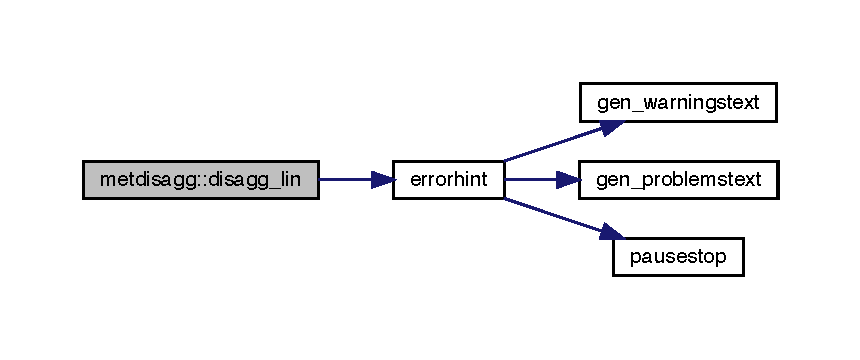
\includegraphics[width=350pt]{namespacemetdisagg_a8ad05f5320b2c1380934b4fbd591bbb9_cgraph}
\end{center}
\end{figure}
\mbox{\Hypertarget{namespacemetdisagg_a68fe3bfaf0b4ea325a7560e9c5ed518a}\label{namespacemetdisagg_a68fe3bfaf0b4ea325a7560e9c5ed518a}} 
\index{metdisagg@{metdisagg}!disaggp\+\_\+amongn@{disaggp\+\_\+amongn}}
\index{disaggp\+\_\+amongn@{disaggp\+\_\+amongn}!metdisagg@{metdisagg}}
\subsubsection{\texorpdfstring{disaggp\+\_\+amongn()}{disaggp\_amongn()}}
{\footnotesize\ttfamily real(kind(1d0)) function, dimension(readlinesorig\+\_\+loc$\ast$nper\+\_\+loc) metdisagg\+::disaggp\+\_\+amongn (\begin{DoxyParamCaption}\item[{real(kind(1d0)), dimension(readlinesorig\+\_\+loc)}]{Slow,  }\item[{integer}]{amongN,  }\item[{integer}]{Nper\+\_\+loc,  }\item[{integer}]{Read\+Lines\+Orig\+\_\+loc,  }\item[{integer}]{Read\+Lines\+Orig\+Max\+\_\+loc }\end{DoxyParamCaption})}



Definition at line 644 of file S\+U\+E\+W\+S\+\_\+\+Met\+Disagg.\+f95.

Here is the call graph for this function\+:\nopagebreak
\begin{figure}[H]
\begin{center}
\leavevmode
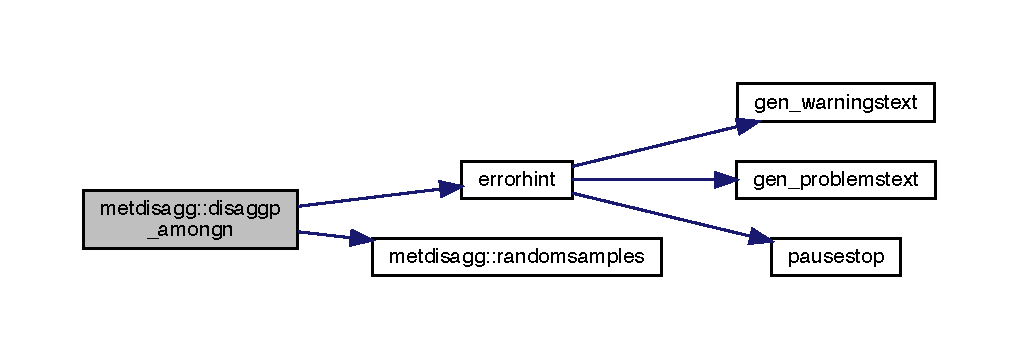
\includegraphics[width=350pt]{namespacemetdisagg_a68fe3bfaf0b4ea325a7560e9c5ed518a_cgraph}
\end{center}
\end{figure}
\mbox{\Hypertarget{namespacemetdisagg_aba0eed0257bc8f0ce67fac76eae7375b}\label{namespacemetdisagg_aba0eed0257bc8f0ce67fac76eae7375b}} 
\index{metdisagg@{metdisagg}!disaggp\+\_\+amongnmult@{disaggp\+\_\+amongnmult}}
\index{disaggp\+\_\+amongnmult@{disaggp\+\_\+amongnmult}!metdisagg@{metdisagg}}
\subsubsection{\texorpdfstring{disaggp\+\_\+amongnmult()}{disaggp\_amongnmult()}}
{\footnotesize\ttfamily real(kind(1d0)) function, dimension(readlinesorig\+\_\+loc$\ast$nper\+\_\+loc) metdisagg\+::disaggp\+\_\+amongnmult (\begin{DoxyParamCaption}\item[{real(kind(1d0)), dimension(readlinesorig\+\_\+loc)}]{Slow,  }\item[{real(kind(1d0)), dimension(5)}]{multupperI,  }\item[{integer, dimension(5)}]{multamongN,  }\item[{integer}]{Nper\+\_\+loc,  }\item[{integer}]{Read\+Lines\+Orig\+\_\+loc,  }\item[{integer}]{Read\+Lines\+Orig\+Max\+\_\+loc }\end{DoxyParamCaption})}



Definition at line 702 of file S\+U\+E\+W\+S\+\_\+\+Met\+Disagg.\+f95.

Here is the call graph for this function\+:\nopagebreak
\begin{figure}[H]
\begin{center}
\leavevmode
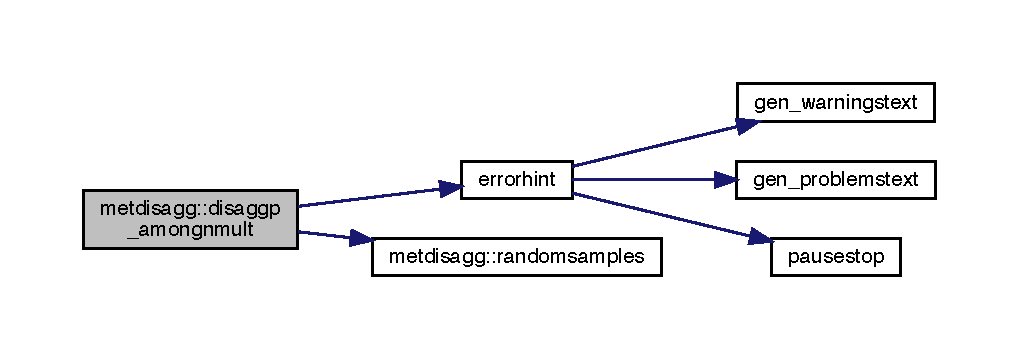
\includegraphics[width=350pt]{namespacemetdisagg_aba0eed0257bc8f0ce67fac76eae7375b_cgraph}
\end{center}
\end{figure}
\mbox{\Hypertarget{namespacemetdisagg_a67b638fd95044f06d411c6866ea8b2be}\label{namespacemetdisagg_a67b638fd95044f06d411c6866ea8b2be}} 
\index{metdisagg@{metdisagg}!disaggregateestm@{disaggregateestm}}
\index{disaggregateestm@{disaggregateestm}!metdisagg@{metdisagg}}
\subsubsection{\texorpdfstring{disaggregateestm()}{disaggregateestm()}}
{\footnotesize\ttfamily subroutine metdisagg\+::disaggregateestm (\begin{DoxyParamCaption}\item[{integer}]{i\+Block }\end{DoxyParamCaption})}



Definition at line 337 of file S\+U\+E\+W\+S\+\_\+\+Met\+Disagg.\+f95.

Here is the call graph for this function\+:\nopagebreak
\begin{figure}[H]
\begin{center}
\leavevmode
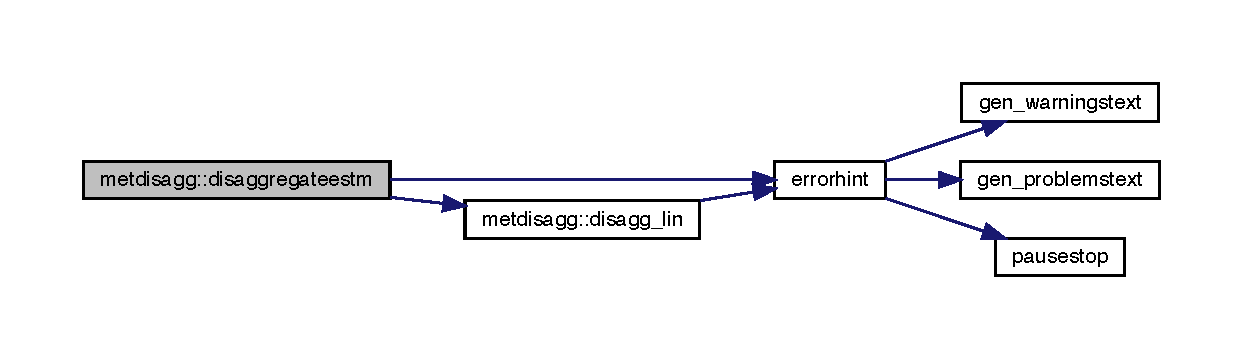
\includegraphics[width=350pt]{namespacemetdisagg_a67b638fd95044f06d411c6866ea8b2be_cgraph}
\end{center}
\end{figure}
\mbox{\Hypertarget{namespacemetdisagg_a9b4db8548b33c73cf14f7280cb8de1b6}\label{namespacemetdisagg_a9b4db8548b33c73cf14f7280cb8de1b6}} 
\index{metdisagg@{metdisagg}!disaggregatemet@{disaggregatemet}}
\index{disaggregatemet@{disaggregatemet}!metdisagg@{metdisagg}}
\subsubsection{\texorpdfstring{disaggregatemet()}{disaggregatemet()}}
{\footnotesize\ttfamily subroutine metdisagg\+::disaggregatemet (\begin{DoxyParamCaption}\item[{integer}]{i\+Block,  }\item[{integer}]{igrid }\end{DoxyParamCaption})}



Definition at line 30 of file S\+U\+E\+W\+S\+\_\+\+Met\+Disagg.\+f95.

Here is the call graph for this function\+:\nopagebreak
\begin{figure}[H]
\begin{center}
\leavevmode
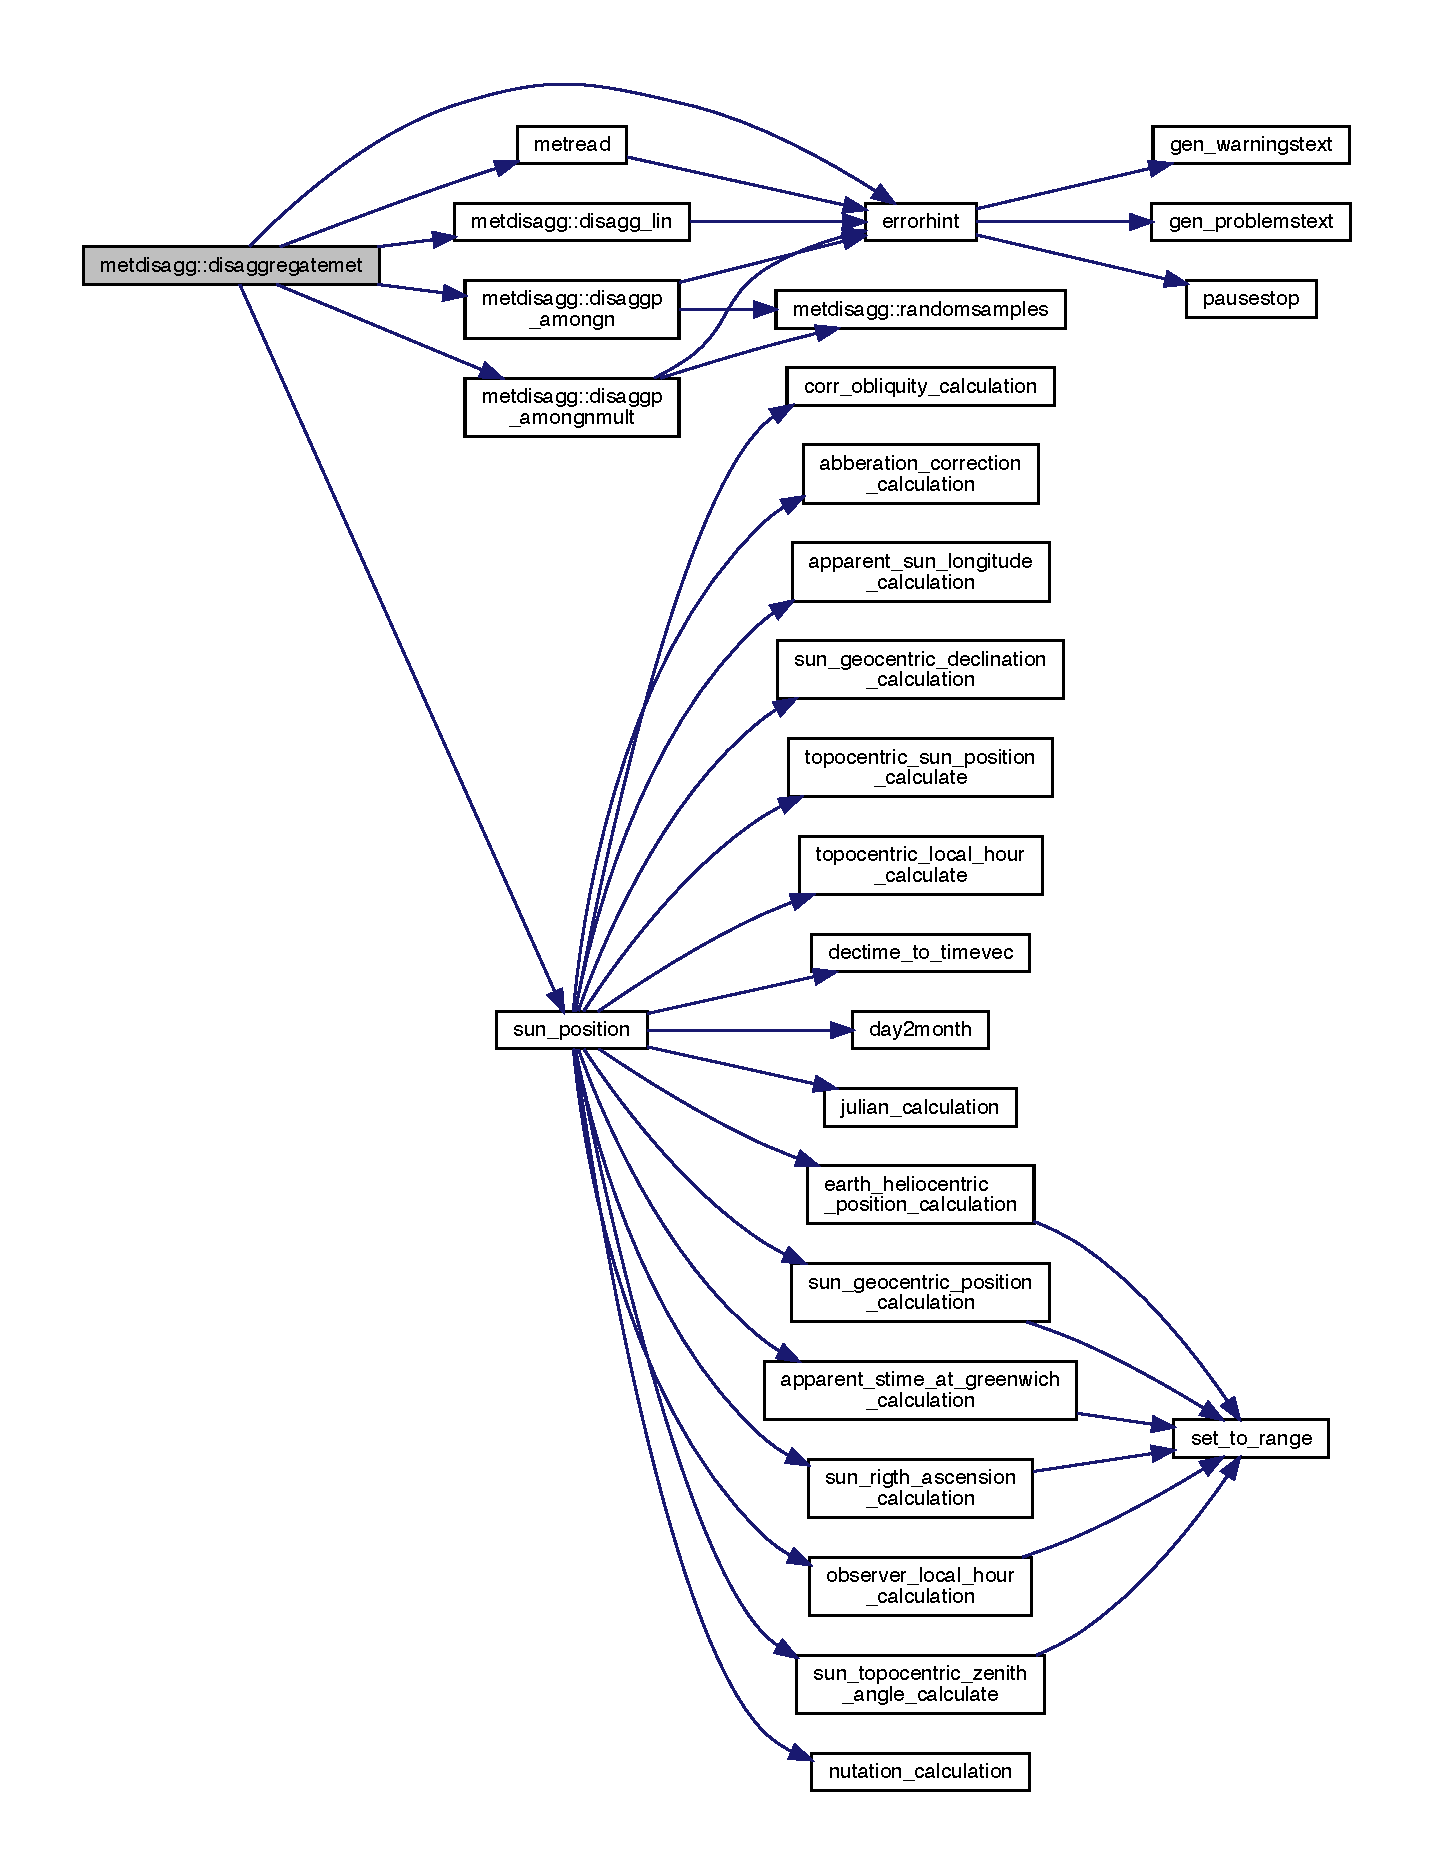
\includegraphics[width=350pt]{namespacemetdisagg_a9b4db8548b33c73cf14f7280cb8de1b6_cgraph}
\end{center}
\end{figure}
\mbox{\Hypertarget{namespacemetdisagg_a23b40d11c1242cb3e4fc0dff94f960db}\label{namespacemetdisagg_a23b40d11c1242cb3e4fc0dff94f960db}} 
\index{metdisagg@{metdisagg}!randomsamples@{randomsamples}}
\index{randomsamples@{randomsamples}!metdisagg@{metdisagg}}
\subsubsection{\texorpdfstring{randomsamples()}{randomsamples()}}
{\footnotesize\ttfamily integer function, dimension(\+:), allocatable metdisagg\+::randomsamples (\begin{DoxyParamCaption}\item[{integer}]{N,  }\item[{integer}]{Out\+Of }\end{DoxyParamCaption})}



Definition at line 778 of file S\+U\+E\+W\+S\+\_\+\+Met\+Disagg.\+f95.


\hypertarget{namespacemeteo}{}\section{meteo Module Reference}
\label{namespacemeteo}\index{meteo@{meteo}}
\subsection*{Functions/\+Subroutines}
\begin{DoxyCompactItemize}
\item 
real(8) function \hyperlink{namespacemeteo_a6777852efdfd10f05bb7467fd99f03ec}{sat\+\_\+vap\+\_\+press} (TK, P)
\item 
real(8) function \hyperlink{namespacemeteo_a799c55d98d43606ee55dfcb2ed973c02}{sos\+\_\+dryair} (TK)
\item 
real(8) function \hyperlink{namespacemeteo_a537068a2255cff524747621cd522b93a}{potential\+\_\+temp} (TK, P)
\item 
real(8) function \hyperlink{namespacemeteo_afaaf9cd39b3f9994813ea6197d3a74bf}{latentheat\+\_\+v} (TK)
\item 
real(8) function \hyperlink{namespacemeteo_a57634c251a493116d57d49865d95c7a6}{latentheat\+\_\+m} (TK)
\item 
real(8) function \hyperlink{namespacemeteo_a1db0e89d35e5eae20acb839111603927}{spec\+\_\+heat\+\_\+dryair} (TK)
\item 
real(8) function \hyperlink{namespacemeteo_a2458549db90b31c67886950a36fe2370}{spec\+\_\+heat\+\_\+vapor} (TK, RH)
\item 
real(8) function \hyperlink{namespacemeteo_a1c0a3877fc85ffd63bbf91b3e710b602}{heatcapacity\+\_\+air} (TK, RH, P)
\item 
real(8) function \hyperlink{namespacemeteo_afeb4cd9d5827418a587e1b78093b08f5}{density\+\_\+moist} (T\+VK, P)
\item 
real(8) function \hyperlink{namespacemeteo_a4a51e0e5cdc190c3e5eccdb69c267382}{density\+\_\+vapor} (TK, RH, P)
\item 
real(8) function \hyperlink{namespacemeteo_a2d3b6838da7330c4e146845991c0bc8a}{density\+\_\+dryair} (TK, P)
\item 
real(8) function \hyperlink{namespacemeteo_a5c26a948b622d4d5ffd1f16f755e3c96}{density\+\_\+gas} (TK, PP, M\+O\+L\+M\+A\+SS)
\item 
real(8) function \hyperlink{namespacemeteo_a0171c7d6a68810bdaa89cb39c92ee96f}{partial\+\_\+pressure} (TK, N)
\item 
real(8) function \hyperlink{namespacemeteo_ad07039dc16c44b421a37a93ec073d7ac}{scale\+\_\+height} (TK)
\item 
real(8) function \hyperlink{namespacemeteo_a60b3a3a3f1d7b40ed8b9fd4b55a9e06b}{vaisala\+\_\+brunt\+\_\+f} (TK)
\end{DoxyCompactItemize}
\subsection*{Variables}
\begin{DoxyCompactItemize}
\item 
real(kind(1d0)), parameter \hyperlink{namespacemeteo_ae4e33b320117dc89986bd1d37a18ae74}{rad2deg} =57.\+29577951
\item 
real(kind(1d0)), parameter \hyperlink{namespacemeteo_a6acb74c9a7ddfe85ba69112897754791}{deg2rad} =0.\+017453292
\item 
real(kind(1d0)), parameter \hyperlink{namespacemeteo_a54b7cd84df1d97cb79965d43460ad694}{molmass\+\_\+air} =0.\+028965
\item 
real(kind(1d0)), parameter \hyperlink{namespacemeteo_acb7ea078c76c3b3d8eed2c1f1df3f6ba}{molmass\+\_\+co2} =0.\+04401
\item 
real(kind(1d0)), parameter \hyperlink{namespacemeteo_aae3f90f9d5c4581ccb0a05acee54f2ac}{molmass\+\_\+h2o} =0.\+0180153
\item 
real(kind(1d0)), parameter \hyperlink{namespacemeteo_ac6780e7f2432c338fc92d3ef2eca5089}{mu\+\_\+h2o} =M\+O\+L\+M\+A\+S\+S\+\_\+\+A\+IR/M\+O\+L\+M\+A\+S\+S\+\_\+\+H2O
\item 
real(kind(1d0)), parameter \hyperlink{namespacemeteo_a5e25bc167da1551976c0f934a28b9c41}{mu\+\_\+co2} =M\+O\+L\+M\+A\+S\+S\+\_\+\+A\+IR/M\+O\+L\+M\+A\+S\+S\+\_\+\+C\+O2
\item 
real(kind(1d0)), parameter \hyperlink{namespacemeteo_a6b0124b140e3a372291310b9c292ceda}{r\+\_\+dry\+\_\+mol} =8.\+31451
\item 
real(kind(1d0)), parameter \hyperlink{namespacemeteo_aeb38e2ee75a5100806164ecfd458a956}{r\+\_\+dry\+\_\+mass} =R\+\_\+\+D\+R\+Y\+\_\+\+M\+OL/M\+O\+L\+M\+A\+S\+S\+\_\+\+A\+IR
\item 
real(kind(1d0)), parameter \hyperlink{namespacemeteo_a63de0dfce55a22ba48600ea13d0e216d}{epsil} =0.\+62197
\item 
real(kind(1d0)), parameter \hyperlink{namespacemeteo_a4ac27cf4384cebc39c7c0ec998ec5579}{kb} =1.\+3807\+E-\/25
\item 
real(kind(1d0)), parameter \hyperlink{namespacemeteo_aaf725e1853e17e82e0db242dcf619c15}{avogadro} =6.\+02252\+E23
\end{DoxyCompactItemize}


\subsection{Function/\+Subroutine Documentation}
\mbox{\Hypertarget{namespacemeteo_a2d3b6838da7330c4e146845991c0bc8a}\label{namespacemeteo_a2d3b6838da7330c4e146845991c0bc8a}} 
\index{meteo@{meteo}!density\+\_\+dryair@{density\+\_\+dryair}}
\index{density\+\_\+dryair@{density\+\_\+dryair}!meteo@{meteo}}
\subsubsection{\texorpdfstring{density\+\_\+dryair()}{density\_dryair()}}
{\footnotesize\ttfamily real(8) function meteo\+::density\+\_\+dryair (\begin{DoxyParamCaption}\item[{real(8)}]{TK,  }\item[{real(8)}]{P }\end{DoxyParamCaption})}



Definition at line 461 of file S\+U\+E\+W\+S\+\_\+\+E\+S\+T\+M\+\_\+functions.\+f95.

\mbox{\Hypertarget{namespacemeteo_a5c26a948b622d4d5ffd1f16f755e3c96}\label{namespacemeteo_a5c26a948b622d4d5ffd1f16f755e3c96}} 
\index{meteo@{meteo}!density\+\_\+gas@{density\+\_\+gas}}
\index{density\+\_\+gas@{density\+\_\+gas}!meteo@{meteo}}
\subsubsection{\texorpdfstring{density\+\_\+gas()}{density\_gas()}}
{\footnotesize\ttfamily real(8) function meteo\+::density\+\_\+gas (\begin{DoxyParamCaption}\item[{real(8)}]{TK,  }\item[{real(8)}]{PP,  }\item[{real(8)}]{M\+O\+L\+M\+A\+SS }\end{DoxyParamCaption})}



Definition at line 466 of file S\+U\+E\+W\+S\+\_\+\+E\+S\+T\+M\+\_\+functions.\+f95.

\mbox{\Hypertarget{namespacemeteo_afeb4cd9d5827418a587e1b78093b08f5}\label{namespacemeteo_afeb4cd9d5827418a587e1b78093b08f5}} 
\index{meteo@{meteo}!density\+\_\+moist@{density\+\_\+moist}}
\index{density\+\_\+moist@{density\+\_\+moist}!meteo@{meteo}}
\subsubsection{\texorpdfstring{density\+\_\+moist()}{density\_moist()}}
{\footnotesize\ttfamily real(8) function meteo\+::density\+\_\+moist (\begin{DoxyParamCaption}\item[{real(8)}]{T\+VK,  }\item[{real(8)}]{P }\end{DoxyParamCaption})}



Definition at line 446 of file S\+U\+E\+W\+S\+\_\+\+E\+S\+T\+M\+\_\+functions.\+f95.

\mbox{\Hypertarget{namespacemeteo_a4a51e0e5cdc190c3e5eccdb69c267382}\label{namespacemeteo_a4a51e0e5cdc190c3e5eccdb69c267382}} 
\index{meteo@{meteo}!density\+\_\+vapor@{density\+\_\+vapor}}
\index{density\+\_\+vapor@{density\+\_\+vapor}!meteo@{meteo}}
\subsubsection{\texorpdfstring{density\+\_\+vapor()}{density\_vapor()}}
{\footnotesize\ttfamily real(8) function meteo\+::density\+\_\+vapor (\begin{DoxyParamCaption}\item[{real(8)}]{TK,  }\item[{real(8)}]{RH,  }\item[{real(8)}]{P }\end{DoxyParamCaption})}



Definition at line 454 of file S\+U\+E\+W\+S\+\_\+\+E\+S\+T\+M\+\_\+functions.\+f95.

Here is the call graph for this function\+:\nopagebreak
\begin{figure}[H]
\begin{center}
\leavevmode
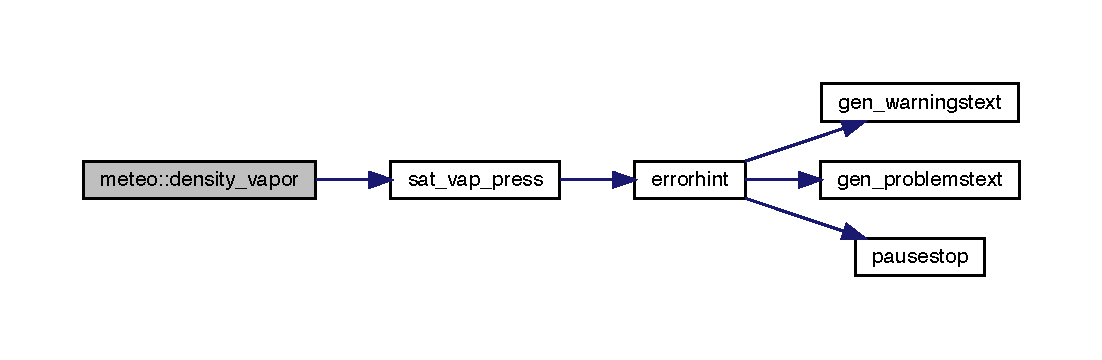
\includegraphics[width=350pt]{namespacemeteo_a4a51e0e5cdc190c3e5eccdb69c267382_cgraph}
\end{center}
\end{figure}
\mbox{\Hypertarget{namespacemeteo_a1c0a3877fc85ffd63bbf91b3e710b602}\label{namespacemeteo_a1c0a3877fc85ffd63bbf91b3e710b602}} 
\index{meteo@{meteo}!heatcapacity\+\_\+air@{heatcapacity\+\_\+air}}
\index{heatcapacity\+\_\+air@{heatcapacity\+\_\+air}!meteo@{meteo}}
\subsubsection{\texorpdfstring{heatcapacity\+\_\+air()}{heatcapacity\_air()}}
{\footnotesize\ttfamily real(8) function meteo\+::heatcapacity\+\_\+air (\begin{DoxyParamCaption}\item[{real(8)}]{TK,  }\item[{real(8)}]{RH,  }\item[{real(8)}]{P }\end{DoxyParamCaption})}



Definition at line 435 of file S\+U\+E\+W\+S\+\_\+\+E\+S\+T\+M\+\_\+functions.\+f95.

Here is the call graph for this function\+:\nopagebreak
\begin{figure}[H]
\begin{center}
\leavevmode
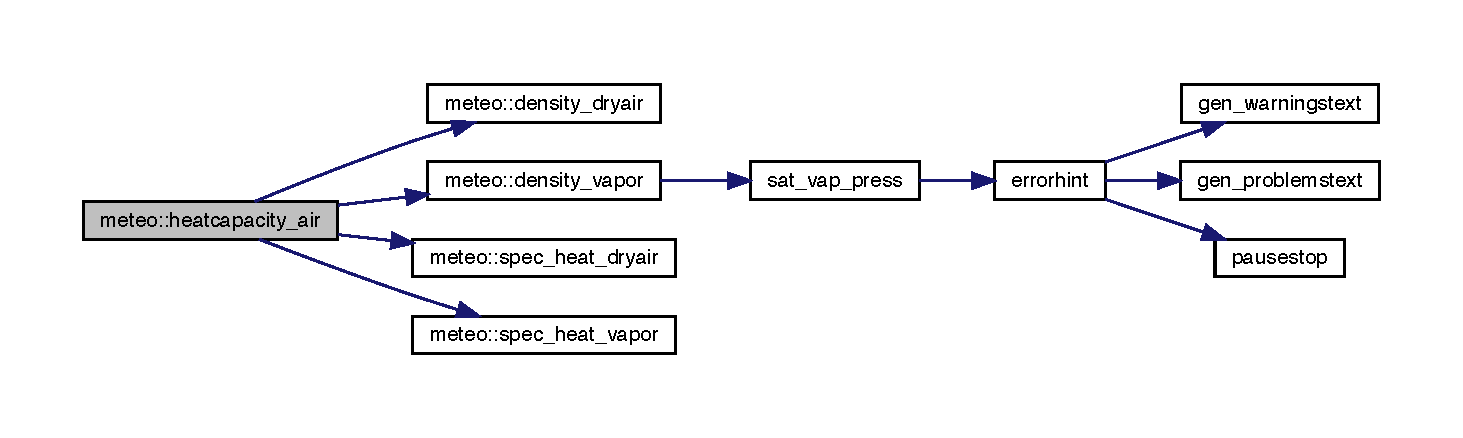
\includegraphics[width=350pt]{namespacemeteo_a1c0a3877fc85ffd63bbf91b3e710b602_cgraph}
\end{center}
\end{figure}
\mbox{\Hypertarget{namespacemeteo_a57634c251a493116d57d49865d95c7a6}\label{namespacemeteo_a57634c251a493116d57d49865d95c7a6}} 
\index{meteo@{meteo}!latentheat\+\_\+m@{latentheat\+\_\+m}}
\index{latentheat\+\_\+m@{latentheat\+\_\+m}!meteo@{meteo}}
\subsubsection{\texorpdfstring{latentheat\+\_\+m()}{latentheat\_m()}}
{\footnotesize\ttfamily real(8) function meteo\+::latentheat\+\_\+m (\begin{DoxyParamCaption}\item[{real(8)}]{TK }\end{DoxyParamCaption})}



Definition at line 413 of file S\+U\+E\+W\+S\+\_\+\+E\+S\+T\+M\+\_\+functions.\+f95.

\mbox{\Hypertarget{namespacemeteo_afaaf9cd39b3f9994813ea6197d3a74bf}\label{namespacemeteo_afaaf9cd39b3f9994813ea6197d3a74bf}} 
\index{meteo@{meteo}!latentheat\+\_\+v@{latentheat\+\_\+v}}
\index{latentheat\+\_\+v@{latentheat\+\_\+v}!meteo@{meteo}}
\subsubsection{\texorpdfstring{latentheat\+\_\+v()}{latentheat\_v()}}
{\footnotesize\ttfamily real(8) function meteo\+::latentheat\+\_\+v (\begin{DoxyParamCaption}\item[{real(8)}]{TK }\end{DoxyParamCaption})}



Definition at line 406 of file S\+U\+E\+W\+S\+\_\+\+E\+S\+T\+M\+\_\+functions.\+f95.

\mbox{\Hypertarget{namespacemeteo_a0171c7d6a68810bdaa89cb39c92ee96f}\label{namespacemeteo_a0171c7d6a68810bdaa89cb39c92ee96f}} 
\index{meteo@{meteo}!partial\+\_\+pressure@{partial\+\_\+pressure}}
\index{partial\+\_\+pressure@{partial\+\_\+pressure}!meteo@{meteo}}
\subsubsection{\texorpdfstring{partial\+\_\+pressure()}{partial\_pressure()}}
{\footnotesize\ttfamily real(8) function meteo\+::partial\+\_\+pressure (\begin{DoxyParamCaption}\item[{real(8)}]{TK,  }\item[{real(8)}]{N }\end{DoxyParamCaption})}



Definition at line 472 of file S\+U\+E\+W\+S\+\_\+\+E\+S\+T\+M\+\_\+functions.\+f95.

\mbox{\Hypertarget{namespacemeteo_a537068a2255cff524747621cd522b93a}\label{namespacemeteo_a537068a2255cff524747621cd522b93a}} 
\index{meteo@{meteo}!potential\+\_\+temp@{potential\+\_\+temp}}
\index{potential\+\_\+temp@{potential\+\_\+temp}!meteo@{meteo}}
\subsubsection{\texorpdfstring{potential\+\_\+temp()}{potential\_temp()}}
{\footnotesize\ttfamily real(8) function meteo\+::potential\+\_\+temp (\begin{DoxyParamCaption}\item[{real(8)}]{TK,  }\item[{real(8)}]{P }\end{DoxyParamCaption})}



Definition at line 399 of file S\+U\+E\+W\+S\+\_\+\+E\+S\+T\+M\+\_\+functions.\+f95.

\mbox{\Hypertarget{namespacemeteo_a6777852efdfd10f05bb7467fd99f03ec}\label{namespacemeteo_a6777852efdfd10f05bb7467fd99f03ec}} 
\index{meteo@{meteo}!sat\+\_\+vap\+\_\+press@{sat\+\_\+vap\+\_\+press}}
\index{sat\+\_\+vap\+\_\+press@{sat\+\_\+vap\+\_\+press}!meteo@{meteo}}
\subsubsection{\texorpdfstring{sat\+\_\+vap\+\_\+press()}{sat\_vap\_press()}}
{\footnotesize\ttfamily real(8) function meteo\+::sat\+\_\+vap\+\_\+press (\begin{DoxyParamCaption}\item[{real(8)}]{TK,  }\item[{real(8)}]{P }\end{DoxyParamCaption})}



Definition at line 377 of file S\+U\+E\+W\+S\+\_\+\+E\+S\+T\+M\+\_\+functions.\+f95.

\mbox{\Hypertarget{namespacemeteo_ad07039dc16c44b421a37a93ec073d7ac}\label{namespacemeteo_ad07039dc16c44b421a37a93ec073d7ac}} 
\index{meteo@{meteo}!scale\+\_\+height@{scale\+\_\+height}}
\index{scale\+\_\+height@{scale\+\_\+height}!meteo@{meteo}}
\subsubsection{\texorpdfstring{scale\+\_\+height()}{scale\_height()}}
{\footnotesize\ttfamily real(8) function meteo\+::scale\+\_\+height (\begin{DoxyParamCaption}\item[{real(8)}]{TK }\end{DoxyParamCaption})}



Definition at line 478 of file S\+U\+E\+W\+S\+\_\+\+E\+S\+T\+M\+\_\+functions.\+f95.

\mbox{\Hypertarget{namespacemeteo_a799c55d98d43606ee55dfcb2ed973c02}\label{namespacemeteo_a799c55d98d43606ee55dfcb2ed973c02}} 
\index{meteo@{meteo}!sos\+\_\+dryair@{sos\+\_\+dryair}}
\index{sos\+\_\+dryair@{sos\+\_\+dryair}!meteo@{meteo}}
\subsubsection{\texorpdfstring{sos\+\_\+dryair()}{sos\_dryair()}}
{\footnotesize\ttfamily real(8) function meteo\+::sos\+\_\+dryair (\begin{DoxyParamCaption}\item[{real(8)}]{TK }\end{DoxyParamCaption})}



Definition at line 393 of file S\+U\+E\+W\+S\+\_\+\+E\+S\+T\+M\+\_\+functions.\+f95.

\mbox{\Hypertarget{namespacemeteo_a1db0e89d35e5eae20acb839111603927}\label{namespacemeteo_a1db0e89d35e5eae20acb839111603927}} 
\index{meteo@{meteo}!spec\+\_\+heat\+\_\+dryair@{spec\+\_\+heat\+\_\+dryair}}
\index{spec\+\_\+heat\+\_\+dryair@{spec\+\_\+heat\+\_\+dryair}!meteo@{meteo}}
\subsubsection{\texorpdfstring{spec\+\_\+heat\+\_\+dryair()}{spec\_heat\_dryair()}}
{\footnotesize\ttfamily real(8) function meteo\+::spec\+\_\+heat\+\_\+dryair (\begin{DoxyParamCaption}\item[{real(8)}]{TK }\end{DoxyParamCaption})}



Definition at line 421 of file S\+U\+E\+W\+S\+\_\+\+E\+S\+T\+M\+\_\+functions.\+f95.

\mbox{\Hypertarget{namespacemeteo_a2458549db90b31c67886950a36fe2370}\label{namespacemeteo_a2458549db90b31c67886950a36fe2370}} 
\index{meteo@{meteo}!spec\+\_\+heat\+\_\+vapor@{spec\+\_\+heat\+\_\+vapor}}
\index{spec\+\_\+heat\+\_\+vapor@{spec\+\_\+heat\+\_\+vapor}!meteo@{meteo}}
\subsubsection{\texorpdfstring{spec\+\_\+heat\+\_\+vapor()}{spec\_heat\_vapor()}}
{\footnotesize\ttfamily real(8) function meteo\+::spec\+\_\+heat\+\_\+vapor (\begin{DoxyParamCaption}\item[{real(8)}]{TK,  }\item[{real(8)}]{RH }\end{DoxyParamCaption})}



Definition at line 428 of file S\+U\+E\+W\+S\+\_\+\+E\+S\+T\+M\+\_\+functions.\+f95.

\mbox{\Hypertarget{namespacemeteo_a60b3a3a3f1d7b40ed8b9fd4b55a9e06b}\label{namespacemeteo_a60b3a3a3f1d7b40ed8b9fd4b55a9e06b}} 
\index{meteo@{meteo}!vaisala\+\_\+brunt\+\_\+f@{vaisala\+\_\+brunt\+\_\+f}}
\index{vaisala\+\_\+brunt\+\_\+f@{vaisala\+\_\+brunt\+\_\+f}!meteo@{meteo}}
\subsubsection{\texorpdfstring{vaisala\+\_\+brunt\+\_\+f()}{vaisala\_brunt\_f()}}
{\footnotesize\ttfamily real(8) function meteo\+::vaisala\+\_\+brunt\+\_\+f (\begin{DoxyParamCaption}\item[{real(8)}]{TK }\end{DoxyParamCaption})}



Definition at line 484 of file S\+U\+E\+W\+S\+\_\+\+E\+S\+T\+M\+\_\+functions.\+f95.

Here is the call graph for this function\+:\nopagebreak
\begin{figure}[H]
\begin{center}
\leavevmode
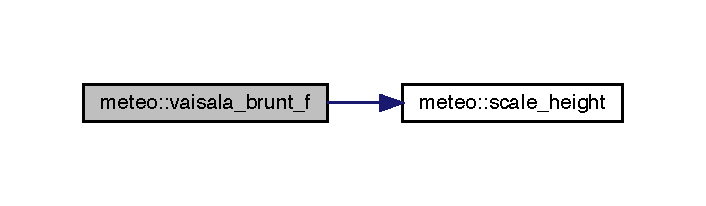
\includegraphics[width=339pt]{namespacemeteo_a60b3a3a3f1d7b40ed8b9fd4b55a9e06b_cgraph}
\end{center}
\end{figure}


\subsection{Variable Documentation}
\mbox{\Hypertarget{namespacemeteo_aaf725e1853e17e82e0db242dcf619c15}\label{namespacemeteo_aaf725e1853e17e82e0db242dcf619c15}} 
\index{meteo@{meteo}!avogadro@{avogadro}}
\index{avogadro@{avogadro}!meteo@{meteo}}
\subsubsection{\texorpdfstring{avogadro}{avogadro}}
{\footnotesize\ttfamily real (kind(1d0)), parameter meteo\+::avogadro =6.\+02252\+E23}



Definition at line 371 of file S\+U\+E\+W\+S\+\_\+\+E\+S\+T\+M\+\_\+functions.\+f95.

\mbox{\Hypertarget{namespacemeteo_a6acb74c9a7ddfe85ba69112897754791}\label{namespacemeteo_a6acb74c9a7ddfe85ba69112897754791}} 
\index{meteo@{meteo}!deg2rad@{deg2rad}}
\index{deg2rad@{deg2rad}!meteo@{meteo}}
\subsubsection{\texorpdfstring{deg2rad}{deg2rad}}
{\footnotesize\ttfamily real (kind(1d0)), parameter meteo\+::deg2rad =0.\+017453292}



Definition at line 359 of file S\+U\+E\+W\+S\+\_\+\+E\+S\+T\+M\+\_\+functions.\+f95.

\mbox{\Hypertarget{namespacemeteo_a63de0dfce55a22ba48600ea13d0e216d}\label{namespacemeteo_a63de0dfce55a22ba48600ea13d0e216d}} 
\index{meteo@{meteo}!epsil@{epsil}}
\index{epsil@{epsil}!meteo@{meteo}}
\subsubsection{\texorpdfstring{epsil}{epsil}}
{\footnotesize\ttfamily real (kind(1d0)), parameter meteo\+::epsil =0.\+62197}



Definition at line 369 of file S\+U\+E\+W\+S\+\_\+\+E\+S\+T\+M\+\_\+functions.\+f95.

\mbox{\Hypertarget{namespacemeteo_a4ac27cf4384cebc39c7c0ec998ec5579}\label{namespacemeteo_a4ac27cf4384cebc39c7c0ec998ec5579}} 
\index{meteo@{meteo}!kb@{kb}}
\index{kb@{kb}!meteo@{meteo}}
\subsubsection{\texorpdfstring{kb}{kb}}
{\footnotesize\ttfamily real (kind(1d0)), parameter meteo\+::kb =1.\+3807\+E-\/25}



Definition at line 370 of file S\+U\+E\+W\+S\+\_\+\+E\+S\+T\+M\+\_\+functions.\+f95.

\mbox{\Hypertarget{namespacemeteo_a54b7cd84df1d97cb79965d43460ad694}\label{namespacemeteo_a54b7cd84df1d97cb79965d43460ad694}} 
\index{meteo@{meteo}!molmass\+\_\+air@{molmass\+\_\+air}}
\index{molmass\+\_\+air@{molmass\+\_\+air}!meteo@{meteo}}
\subsubsection{\texorpdfstring{molmass\+\_\+air}{molmass\_air}}
{\footnotesize\ttfamily real (kind(1d0)), parameter meteo\+::molmass\+\_\+air =0.\+028965}



Definition at line 361 of file S\+U\+E\+W\+S\+\_\+\+E\+S\+T\+M\+\_\+functions.\+f95.

\mbox{\Hypertarget{namespacemeteo_acb7ea078c76c3b3d8eed2c1f1df3f6ba}\label{namespacemeteo_acb7ea078c76c3b3d8eed2c1f1df3f6ba}} 
\index{meteo@{meteo}!molmass\+\_\+co2@{molmass\+\_\+co2}}
\index{molmass\+\_\+co2@{molmass\+\_\+co2}!meteo@{meteo}}
\subsubsection{\texorpdfstring{molmass\+\_\+co2}{molmass\_co2}}
{\footnotesize\ttfamily real (kind(1d0)), parameter meteo\+::molmass\+\_\+co2 =0.\+04401}



Definition at line 362 of file S\+U\+E\+W\+S\+\_\+\+E\+S\+T\+M\+\_\+functions.\+f95.

\mbox{\Hypertarget{namespacemeteo_aae3f90f9d5c4581ccb0a05acee54f2ac}\label{namespacemeteo_aae3f90f9d5c4581ccb0a05acee54f2ac}} 
\index{meteo@{meteo}!molmass\+\_\+h2o@{molmass\+\_\+h2o}}
\index{molmass\+\_\+h2o@{molmass\+\_\+h2o}!meteo@{meteo}}
\subsubsection{\texorpdfstring{molmass\+\_\+h2o}{molmass\_h2o}}
{\footnotesize\ttfamily real (kind(1d0)), parameter meteo\+::molmass\+\_\+h2o =0.\+0180153}



Definition at line 363 of file S\+U\+E\+W\+S\+\_\+\+E\+S\+T\+M\+\_\+functions.\+f95.

\mbox{\Hypertarget{namespacemeteo_a5e25bc167da1551976c0f934a28b9c41}\label{namespacemeteo_a5e25bc167da1551976c0f934a28b9c41}} 
\index{meteo@{meteo}!mu\+\_\+co2@{mu\+\_\+co2}}
\index{mu\+\_\+co2@{mu\+\_\+co2}!meteo@{meteo}}
\subsubsection{\texorpdfstring{mu\+\_\+co2}{mu\_co2}}
{\footnotesize\ttfamily real (kind(1d0)), parameter meteo\+::mu\+\_\+co2 =M\+O\+L\+M\+A\+S\+S\+\_\+\+A\+IR/M\+O\+L\+M\+A\+S\+S\+\_\+\+C\+O2}



Definition at line 365 of file S\+U\+E\+W\+S\+\_\+\+E\+S\+T\+M\+\_\+functions.\+f95.

\mbox{\Hypertarget{namespacemeteo_ac6780e7f2432c338fc92d3ef2eca5089}\label{namespacemeteo_ac6780e7f2432c338fc92d3ef2eca5089}} 
\index{meteo@{meteo}!mu\+\_\+h2o@{mu\+\_\+h2o}}
\index{mu\+\_\+h2o@{mu\+\_\+h2o}!meteo@{meteo}}
\subsubsection{\texorpdfstring{mu\+\_\+h2o}{mu\_h2o}}
{\footnotesize\ttfamily real (kind(1d0)), parameter meteo\+::mu\+\_\+h2o =M\+O\+L\+M\+A\+S\+S\+\_\+\+A\+IR/M\+O\+L\+M\+A\+S\+S\+\_\+\+H2O}



Definition at line 364 of file S\+U\+E\+W\+S\+\_\+\+E\+S\+T\+M\+\_\+functions.\+f95.

\mbox{\Hypertarget{namespacemeteo_aeb38e2ee75a5100806164ecfd458a956}\label{namespacemeteo_aeb38e2ee75a5100806164ecfd458a956}} 
\index{meteo@{meteo}!r\+\_\+dry\+\_\+mass@{r\+\_\+dry\+\_\+mass}}
\index{r\+\_\+dry\+\_\+mass@{r\+\_\+dry\+\_\+mass}!meteo@{meteo}}
\subsubsection{\texorpdfstring{r\+\_\+dry\+\_\+mass}{r\_dry\_mass}}
{\footnotesize\ttfamily real (kind(1d0)), parameter meteo\+::r\+\_\+dry\+\_\+mass =R\+\_\+\+D\+R\+Y\+\_\+\+M\+OL/M\+O\+L\+M\+A\+S\+S\+\_\+\+A\+IR}



Definition at line 367 of file S\+U\+E\+W\+S\+\_\+\+E\+S\+T\+M\+\_\+functions.\+f95.

\mbox{\Hypertarget{namespacemeteo_a6b0124b140e3a372291310b9c292ceda}\label{namespacemeteo_a6b0124b140e3a372291310b9c292ceda}} 
\index{meteo@{meteo}!r\+\_\+dry\+\_\+mol@{r\+\_\+dry\+\_\+mol}}
\index{r\+\_\+dry\+\_\+mol@{r\+\_\+dry\+\_\+mol}!meteo@{meteo}}
\subsubsection{\texorpdfstring{r\+\_\+dry\+\_\+mol}{r\_dry\_mol}}
{\footnotesize\ttfamily real (kind(1d0)), parameter meteo\+::r\+\_\+dry\+\_\+mol =8.\+31451}



Definition at line 366 of file S\+U\+E\+W\+S\+\_\+\+E\+S\+T\+M\+\_\+functions.\+f95.

\mbox{\Hypertarget{namespacemeteo_ae4e33b320117dc89986bd1d37a18ae74}\label{namespacemeteo_ae4e33b320117dc89986bd1d37a18ae74}} 
\index{meteo@{meteo}!rad2deg@{rad2deg}}
\index{rad2deg@{rad2deg}!meteo@{meteo}}
\subsubsection{\texorpdfstring{rad2deg}{rad2deg}}
{\footnotesize\ttfamily real (kind(1d0)), parameter meteo\+::rad2deg =57.\+29577951}



Definition at line 358 of file S\+U\+E\+W\+S\+\_\+\+E\+S\+T\+M\+\_\+functions.\+f95.


\hypertarget{namespacemod__grav}{}\section{mod\+\_\+grav Module Reference}
\label{namespacemod__grav}\index{mod\+\_\+grav@{mod\+\_\+grav}}
\subsection*{Variables}
\begin{DoxyCompactItemize}
\item 
real(kind(1d0)) \hyperlink{namespacemod__grav_a582b71e075d46273d35f8b2f62ae8aec}{grav} =9.\+80665
\end{DoxyCompactItemize}


\subsection{Variable Documentation}
\mbox{\Hypertarget{namespacemod__grav_a582b71e075d46273d35f8b2f62ae8aec}\label{namespacemod__grav_a582b71e075d46273d35f8b2f62ae8aec}} 
\index{mod\+\_\+grav@{mod\+\_\+grav}!grav@{grav}}
\index{grav@{grav}!mod\+\_\+grav@{mod\+\_\+grav}}
\subsubsection{\texorpdfstring{grav}{grav}}
{\footnotesize\ttfamily real (kind(1d0)) mod\+\_\+grav\+::grav =9.\+80665}



Definition at line 1164 of file L\+U\+M\+P\+S\+\_\+\+Module\+\_\+constants.\+f95.


\hypertarget{namespacemod__interp}{}\section{mod\+\_\+interp Module Reference}
\label{namespacemod__interp}\index{mod\+\_\+interp@{mod\+\_\+interp}}
\subsection*{Functions/\+Subroutines}
\begin{DoxyCompactItemize}
\item 
elemental real(8) function \hyperlink{namespacemod__interp_aa2652ff1ded2f432b31108bd81c6dbd6}{interp1d} (x1, x2, y1, y2, xi)
\end{DoxyCompactItemize}


\subsection{Function/\+Subroutine Documentation}
\mbox{\Hypertarget{namespacemod__interp_aa2652ff1ded2f432b31108bd81c6dbd6}\label{namespacemod__interp_aa2652ff1ded2f432b31108bd81c6dbd6}} 
\index{mod\+\_\+interp@{mod\+\_\+interp}!interp1d@{interp1d}}
\index{interp1d@{interp1d}!mod\+\_\+interp@{mod\+\_\+interp}}
\subsubsection{\texorpdfstring{interp1d()}{interp1d()}}
{\footnotesize\ttfamily elemental real(8) function mod\+\_\+interp\+::interp1d (\begin{DoxyParamCaption}\item[{real(8), intent(in)}]{x1,  }\item[{real(8), intent(in)}]{x2,  }\item[{real(8), intent(in)}]{y1,  }\item[{real(8), intent(in)}]{y2,  }\item[{real(8), intent(in)}]{xi }\end{DoxyParamCaption})}



Definition at line 26 of file S\+U\+E\+W\+S\+\_\+\+E\+S\+T\+M\+\_\+functions.\+f95.


\hypertarget{namespacemod__k}{}\section{mod\+\_\+k Module Reference}
\label{namespacemod__k}\index{mod\+\_\+k@{mod\+\_\+k}}
\subsection*{Variables}
\begin{DoxyCompactItemize}
\item 
real(kind(1d0)) \hyperlink{namespacemod__k_a75bb9b4e883eadeb3233662441943aaf}{k} =0.\+4
\item 
real(kind(1d0)) \hyperlink{namespacemod__k_a85838ba0577d2383b8c545d028333e48}{k2} =0.\+16
\item 
real(kind(1d0)) \hyperlink{namespacemod__k_a22d2aee55ef526b3cae06021044b7ae0}{neut\+\_\+limit} =0.\+001000
\end{DoxyCompactItemize}


\subsection{Variable Documentation}
\mbox{\Hypertarget{namespacemod__k_a75bb9b4e883eadeb3233662441943aaf}\label{namespacemod__k_a75bb9b4e883eadeb3233662441943aaf}} 
\index{mod\+\_\+k@{mod\+\_\+k}!k@{k}}
\index{k@{k}!mod\+\_\+k@{mod\+\_\+k}}
\subsubsection{\texorpdfstring{k}{k}}
{\footnotesize\ttfamily real(kind(1d0)) mod\+\_\+k\+::k =0.\+4}



Definition at line 1169 of file L\+U\+M\+P\+S\+\_\+\+Module\+\_\+constants.\+f95.

\mbox{\Hypertarget{namespacemod__k_a85838ba0577d2383b8c545d028333e48}\label{namespacemod__k_a85838ba0577d2383b8c545d028333e48}} 
\index{mod\+\_\+k@{mod\+\_\+k}!k2@{k2}}
\index{k2@{k2}!mod\+\_\+k@{mod\+\_\+k}}
\subsubsection{\texorpdfstring{k2}{k2}}
{\footnotesize\ttfamily real(kind(1d0)) mod\+\_\+k\+::k2 =0.\+16}



Definition at line 1169 of file L\+U\+M\+P\+S\+\_\+\+Module\+\_\+constants.\+f95.

\mbox{\Hypertarget{namespacemod__k_a22d2aee55ef526b3cae06021044b7ae0}\label{namespacemod__k_a22d2aee55ef526b3cae06021044b7ae0}} 
\index{mod\+\_\+k@{mod\+\_\+k}!neut\+\_\+limit@{neut\+\_\+limit}}
\index{neut\+\_\+limit@{neut\+\_\+limit}!mod\+\_\+k@{mod\+\_\+k}}
\subsubsection{\texorpdfstring{neut\+\_\+limit}{neut\_limit}}
{\footnotesize\ttfamily real(kind(1d0)) mod\+\_\+k\+::neut\+\_\+limit =0.\+001000}



Definition at line 1169 of file L\+U\+M\+P\+S\+\_\+\+Module\+\_\+constants.\+f95.


\hypertarget{namespacemod__solver}{}\section{mod\+\_\+solver Module Reference}
\label{namespacemod__solver}\index{mod\+\_\+solver@{mod\+\_\+solver}}
\subsection*{Functions/\+Subroutines}
\begin{DoxyCompactItemize}
\item 
real(8) function \hyperlink{namespacemod__solver_a7906d5a56feebc123a09f0898a0a54e5}{newtonpolynomial} (x0, Pcoeff, conv, maxiter)
\end{DoxyCompactItemize}


\subsection{Function/\+Subroutine Documentation}
\mbox{\Hypertarget{namespacemod__solver_a7906d5a56feebc123a09f0898a0a54e5}\label{namespacemod__solver_a7906d5a56feebc123a09f0898a0a54e5}} 
\index{mod\+\_\+solver@{mod\+\_\+solver}!newtonpolynomial@{newtonpolynomial}}
\index{newtonpolynomial@{newtonpolynomial}!mod\+\_\+solver@{mod\+\_\+solver}}
\subsubsection{\texorpdfstring{newtonpolynomial()}{newtonpolynomial()}}
{\footnotesize\ttfamily real(8) function mod\+\_\+solver\+::newtonpolynomial (\begin{DoxyParamCaption}\item[{real(8)}]{x0,  }\item[{real(8), dimension(\+:)}]{Pcoeff,  }\item[{real(8)}]{conv,  }\item[{integer}]{maxiter }\end{DoxyParamCaption})}



Definition at line 47 of file S\+U\+E\+W\+S\+\_\+\+E\+S\+T\+M\+\_\+functions.\+f95.


\hypertarget{namespacemod__z}{}\section{mod\+\_\+z Module Reference}
\label{namespacemod__z}\index{mod\+\_\+z@{mod\+\_\+z}}
\subsection*{Variables}
\begin{DoxyCompactItemize}
\item 
real(kind(1d0)) \hyperlink{namespacemod__z_ac1314dbe1ed7b4c92c501ced67f725c3}{zzd}
\item 
real(kind(1d0)) \hyperlink{namespacemod__z_afd15a8bab419b8b576ccd3fa639d546f}{z0m}
\item 
real(kind(1d0)) \hyperlink{namespacemod__z_a85318ac2a4eb1313fc10432ff860214e}{zdm}
\item 
real(kind(1d0)) \hyperlink{namespacemod__z_a64eb68f633930155dd1415ee7f3e9d5c}{z}
\item 
real(kind(1e10)) \hyperlink{namespacemod__z_a62697e7e7a6c6a41258386a4a26ec1a7}{z0v}
\end{DoxyCompactItemize}


\subsection{Variable Documentation}
\mbox{\Hypertarget{namespacemod__z_a64eb68f633930155dd1415ee7f3e9d5c}\label{namespacemod__z_a64eb68f633930155dd1415ee7f3e9d5c}} 
\index{mod\+\_\+z@{mod\+\_\+z}!z@{z}}
\index{z@{z}!mod\+\_\+z@{mod\+\_\+z}}
\subsubsection{\texorpdfstring{z}{z}}
{\footnotesize\ttfamily real (kind(1d0)) mod\+\_\+z\+::z}



Definition at line 1198 of file L\+U\+M\+P\+S\+\_\+\+Module\+\_\+constants.\+f95.

\mbox{\Hypertarget{namespacemod__z_afd15a8bab419b8b576ccd3fa639d546f}\label{namespacemod__z_afd15a8bab419b8b576ccd3fa639d546f}} 
\index{mod\+\_\+z@{mod\+\_\+z}!z0m@{z0m}}
\index{z0m@{z0m}!mod\+\_\+z@{mod\+\_\+z}}
\subsubsection{\texorpdfstring{z0m}{z0m}}
{\footnotesize\ttfamily real (kind(1d0)) mod\+\_\+z\+::z0m}



Definition at line 1198 of file L\+U\+M\+P\+S\+\_\+\+Module\+\_\+constants.\+f95.

\mbox{\Hypertarget{namespacemod__z_a62697e7e7a6c6a41258386a4a26ec1a7}\label{namespacemod__z_a62697e7e7a6c6a41258386a4a26ec1a7}} 
\index{mod\+\_\+z@{mod\+\_\+z}!z0v@{z0v}}
\index{z0v@{z0v}!mod\+\_\+z@{mod\+\_\+z}}
\subsubsection{\texorpdfstring{z0v}{z0v}}
{\footnotesize\ttfamily real(kind(1e10)) mod\+\_\+z\+::z0v}



Definition at line 1202 of file L\+U\+M\+P\+S\+\_\+\+Module\+\_\+constants.\+f95.

\mbox{\Hypertarget{namespacemod__z_a85318ac2a4eb1313fc10432ff860214e}\label{namespacemod__z_a85318ac2a4eb1313fc10432ff860214e}} 
\index{mod\+\_\+z@{mod\+\_\+z}!zdm@{zdm}}
\index{zdm@{zdm}!mod\+\_\+z@{mod\+\_\+z}}
\subsubsection{\texorpdfstring{zdm}{zdm}}
{\footnotesize\ttfamily real (kind(1d0)) mod\+\_\+z\+::zdm}



Definition at line 1198 of file L\+U\+M\+P\+S\+\_\+\+Module\+\_\+constants.\+f95.

\mbox{\Hypertarget{namespacemod__z_ac1314dbe1ed7b4c92c501ced67f725c3}\label{namespacemod__z_ac1314dbe1ed7b4c92c501ced67f725c3}} 
\index{mod\+\_\+z@{mod\+\_\+z}!zzd@{zzd}}
\index{zzd@{zzd}!mod\+\_\+z@{mod\+\_\+z}}
\subsubsection{\texorpdfstring{zzd}{zzd}}
{\footnotesize\ttfamily real (kind(1d0)) mod\+\_\+z\+::zzd}



Definition at line 1198 of file L\+U\+M\+P\+S\+\_\+\+Module\+\_\+constants.\+f95.


\hypertarget{namespacemodsolarcalc}{}\section{modsolarcalc Module Reference}
\label{namespacemodsolarcalc}\index{modsolarcalc@{modsolarcalc}}
\subsection*{Functions/\+Subroutines}
\begin{DoxyCompactItemize}
\item 
real(8) function \hyperlink{namespacemodsolarcalc_adfed66792e245bded2293250a0436520}{min\+\_\+zenith} (lat, doy)
\item 
real(8) function \hyperlink{namespacemodsolarcalc_a9ea53ee8fa5b7be8f0e7d919cc846182}{local\+\_\+apparent\+\_\+time} (lng, dectime)
\item 
subroutine \hyperlink{namespacemodsolarcalc_a6f49f02608586154b6a3b3cddcd6aa5e}{solar\+\_\+angles} (lat, lng, timezone, dectime, decl, zenith, azimuth)
\item 
subroutine \hyperlink{namespacemodsolarcalc_a2fbd1d33b3bd03fd930a2a3d93b83599}{solar\+\_\+times} (lat, lng, timezone, dectime, sunrise, sunset, snoon)
\item 
real(8) function \hyperlink{namespacemodsolarcalc_af8c3c752c506d880efae84070a189a71}{kdown\+\_\+surface} (doy, zenith)
\item 
real function, dimension(365) \hyperlink{namespacemodsolarcalc_abf0aac3f480ad1b6dbfdac598c453fa5}{smithlambda} (lat)
\item 
real(8) function \hyperlink{namespacemodsolarcalc_ad567772df0c379c013b1bec090be214a}{transmissivity\+\_\+cd} (P, Td, G, zenith)
\item 
real function \hyperlink{namespacemodsolarcalc_aaddec454c9882fef35b57ee1fa6206b2}{kdown\+\_\+niemala} (S0, vap\+\_\+press, Tk)
\item 
subroutine \hyperlink{namespacemodsolarcalc_a8e5e61f1a3537693aa4ca5527f74233e}{transmissivity} (vap\+\_\+press, Tk, theta, tr, tg, tw, ta, toz)
\item 
real(8) function \hyperlink{namespacemodsolarcalc_a17e233516e1b3514fd9d46a9ebe44e5e}{solar\+\_\+esdist} (doy)
\end{DoxyCompactItemize}


\subsection{Function/\+Subroutine Documentation}
\mbox{\Hypertarget{namespacemodsolarcalc_aaddec454c9882fef35b57ee1fa6206b2}\label{namespacemodsolarcalc_aaddec454c9882fef35b57ee1fa6206b2}} 
\index{modsolarcalc@{modsolarcalc}!kdown\+\_\+niemala@{kdown\+\_\+niemala}}
\index{kdown\+\_\+niemala@{kdown\+\_\+niemala}!modsolarcalc@{modsolarcalc}}
\subsubsection{\texorpdfstring{kdown\+\_\+niemala()}{kdown\_niemala()}}
{\footnotesize\ttfamily real function modsolarcalc\+::kdown\+\_\+niemala (\begin{DoxyParamCaption}\item[{real}]{S0,  }\item[{real}]{vap\+\_\+press,  }\item[{real}]{Tk }\end{DoxyParamCaption})}



Definition at line 250 of file S\+U\+E\+W\+S\+\_\+\+E\+S\+T\+M\+\_\+functions.\+f95.

Here is the call graph for this function\+:\nopagebreak
\begin{figure}[H]
\begin{center}
\leavevmode
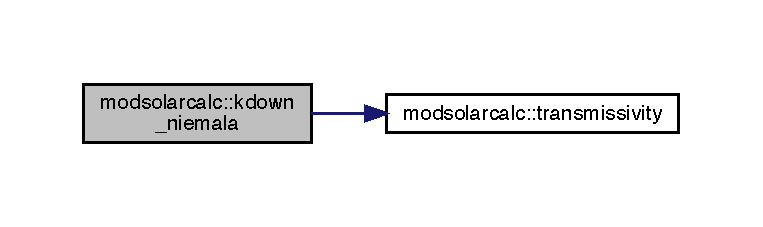
\includegraphics[width=350pt]{namespacemodsolarcalc_aaddec454c9882fef35b57ee1fa6206b2_cgraph}
\end{center}
\end{figure}
\mbox{\Hypertarget{namespacemodsolarcalc_af8c3c752c506d880efae84070a189a71}\label{namespacemodsolarcalc_af8c3c752c506d880efae84070a189a71}} 
\index{modsolarcalc@{modsolarcalc}!kdown\+\_\+surface@{kdown\+\_\+surface}}
\index{kdown\+\_\+surface@{kdown\+\_\+surface}!modsolarcalc@{modsolarcalc}}
\subsubsection{\texorpdfstring{kdown\+\_\+surface()}{kdown\_surface()}}
{\footnotesize\ttfamily real(8) function modsolarcalc\+::kdown\+\_\+surface (\begin{DoxyParamCaption}\item[{integer}]{doy,  }\item[{real(8)}]{zenith }\end{DoxyParamCaption})}



Definition at line 185 of file S\+U\+E\+W\+S\+\_\+\+E\+S\+T\+M\+\_\+functions.\+f95.

Here is the call graph for this function\+:\nopagebreak
\begin{figure}[H]
\begin{center}
\leavevmode
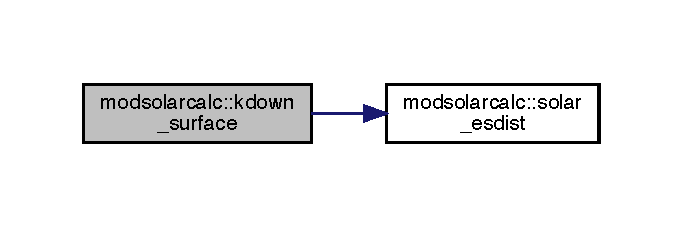
\includegraphics[width=328pt]{namespacemodsolarcalc_af8c3c752c506d880efae84070a189a71_cgraph}
\end{center}
\end{figure}
\mbox{\Hypertarget{namespacemodsolarcalc_a9ea53ee8fa5b7be8f0e7d919cc846182}\label{namespacemodsolarcalc_a9ea53ee8fa5b7be8f0e7d919cc846182}} 
\index{modsolarcalc@{modsolarcalc}!local\+\_\+apparent\+\_\+time@{local\+\_\+apparent\+\_\+time}}
\index{local\+\_\+apparent\+\_\+time@{local\+\_\+apparent\+\_\+time}!modsolarcalc@{modsolarcalc}}
\subsubsection{\texorpdfstring{local\+\_\+apparent\+\_\+time()}{local\_apparent\_time()}}
{\footnotesize\ttfamily real(8) function modsolarcalc\+::local\+\_\+apparent\+\_\+time (\begin{DoxyParamCaption}\item[{real(8)}]{lng,  }\item[{real(8)}]{dectime }\end{DoxyParamCaption})}



Definition at line 116 of file S\+U\+E\+W\+S\+\_\+\+E\+S\+T\+M\+\_\+functions.\+f95.

\mbox{\Hypertarget{namespacemodsolarcalc_adfed66792e245bded2293250a0436520}\label{namespacemodsolarcalc_adfed66792e245bded2293250a0436520}} 
\index{modsolarcalc@{modsolarcalc}!min\+\_\+zenith@{min\+\_\+zenith}}
\index{min\+\_\+zenith@{min\+\_\+zenith}!modsolarcalc@{modsolarcalc}}
\subsubsection{\texorpdfstring{min\+\_\+zenith()}{min\_zenith()}}
{\footnotesize\ttfamily real(8) function modsolarcalc\+::min\+\_\+zenith (\begin{DoxyParamCaption}\item[{real(8)}]{lat,  }\item[{integer}]{doy }\end{DoxyParamCaption})}



Definition at line 102 of file S\+U\+E\+W\+S\+\_\+\+E\+S\+T\+M\+\_\+functions.\+f95.

\mbox{\Hypertarget{namespacemodsolarcalc_abf0aac3f480ad1b6dbfdac598c453fa5}\label{namespacemodsolarcalc_abf0aac3f480ad1b6dbfdac598c453fa5}} 
\index{modsolarcalc@{modsolarcalc}!smithlambda@{smithlambda}}
\index{smithlambda@{smithlambda}!modsolarcalc@{modsolarcalc}}
\subsubsection{\texorpdfstring{smithlambda()}{smithlambda()}}
{\footnotesize\ttfamily real function, dimension(365) modsolarcalc\+::smithlambda (\begin{DoxyParamCaption}\item[{integer}]{lat }\end{DoxyParamCaption})}



Definition at line 206 of file S\+U\+E\+W\+S\+\_\+\+E\+S\+T\+M\+\_\+functions.\+f95.

\mbox{\Hypertarget{namespacemodsolarcalc_a6f49f02608586154b6a3b3cddcd6aa5e}\label{namespacemodsolarcalc_a6f49f02608586154b6a3b3cddcd6aa5e}} 
\index{modsolarcalc@{modsolarcalc}!solar\+\_\+angles@{solar\+\_\+angles}}
\index{solar\+\_\+angles@{solar\+\_\+angles}!modsolarcalc@{modsolarcalc}}
\subsubsection{\texorpdfstring{solar\+\_\+angles()}{solar\_angles()}}
{\footnotesize\ttfamily subroutine modsolarcalc\+::solar\+\_\+angles (\begin{DoxyParamCaption}\item[{real, intent(in)}]{lat,  }\item[{real, intent(in)}]{lng,  }\item[{real, intent(in)}]{timezone,  }\item[{real, intent(in)}]{dectime,  }\item[{real(8), intent(out)}]{decl,  }\item[{real(8), intent(out)}]{zenith,  }\item[{real(8), intent(out)}]{azimuth }\end{DoxyParamCaption})}



Definition at line 129 of file S\+U\+E\+W\+S\+\_\+\+E\+S\+T\+M\+\_\+functions.\+f95.

\mbox{\Hypertarget{namespacemodsolarcalc_a17e233516e1b3514fd9d46a9ebe44e5e}\label{namespacemodsolarcalc_a17e233516e1b3514fd9d46a9ebe44e5e}} 
\index{modsolarcalc@{modsolarcalc}!solar\+\_\+esdist@{solar\+\_\+esdist}}
\index{solar\+\_\+esdist@{solar\+\_\+esdist}!modsolarcalc@{modsolarcalc}}
\subsubsection{\texorpdfstring{solar\+\_\+esdist()}{solar\_esdist()}}
{\footnotesize\ttfamily real(8) function modsolarcalc\+::solar\+\_\+esdist (\begin{DoxyParamCaption}\item[{integer}]{doy }\end{DoxyParamCaption})}



Definition at line 295 of file S\+U\+E\+W\+S\+\_\+\+E\+S\+T\+M\+\_\+functions.\+f95.

\mbox{\Hypertarget{namespacemodsolarcalc_a2fbd1d33b3bd03fd930a2a3d93b83599}\label{namespacemodsolarcalc_a2fbd1d33b3bd03fd930a2a3d93b83599}} 
\index{modsolarcalc@{modsolarcalc}!solar\+\_\+times@{solar\+\_\+times}}
\index{solar\+\_\+times@{solar\+\_\+times}!modsolarcalc@{modsolarcalc}}
\subsubsection{\texorpdfstring{solar\+\_\+times()}{solar\_times()}}
{\footnotesize\ttfamily subroutine modsolarcalc\+::solar\+\_\+times (\begin{DoxyParamCaption}\item[{real(8), intent(in)}]{lat,  }\item[{real(8), intent(in)}]{lng,  }\item[{real(8), intent(in)}]{timezone,  }\item[{real(8), intent(in)}]{dectime,  }\item[{real(8), intent(out)}]{sunrise,  }\item[{real(8), intent(out)}]{sunset,  }\item[{real(8), intent(out)}]{snoon }\end{DoxyParamCaption})}



Definition at line 160 of file S\+U\+E\+W\+S\+\_\+\+E\+S\+T\+M\+\_\+functions.\+f95.

\mbox{\Hypertarget{namespacemodsolarcalc_a8e5e61f1a3537693aa4ca5527f74233e}\label{namespacemodsolarcalc_a8e5e61f1a3537693aa4ca5527f74233e}} 
\index{modsolarcalc@{modsolarcalc}!transmissivity@{transmissivity}}
\index{transmissivity@{transmissivity}!modsolarcalc@{modsolarcalc}}
\subsubsection{\texorpdfstring{transmissivity()}{transmissivity()}}
{\footnotesize\ttfamily subroutine modsolarcalc\+::transmissivity (\begin{DoxyParamCaption}\item[{real}]{vap\+\_\+press,  }\item[{real}]{Tk,  }\item[{real}]{theta,  }\item[{real}]{tr,  }\item[{real}]{tg,  }\item[{real}]{tw,  }\item[{real}]{ta,  }\item[{real}]{toz }\end{DoxyParamCaption})}



Definition at line 276 of file S\+U\+E\+W\+S\+\_\+\+E\+S\+T\+M\+\_\+functions.\+f95.

\mbox{\Hypertarget{namespacemodsolarcalc_ad567772df0c379c013b1bec090be214a}\label{namespacemodsolarcalc_ad567772df0c379c013b1bec090be214a}} 
\index{modsolarcalc@{modsolarcalc}!transmissivity\+\_\+cd@{transmissivity\+\_\+cd}}
\index{transmissivity\+\_\+cd@{transmissivity\+\_\+cd}!modsolarcalc@{modsolarcalc}}
\subsubsection{\texorpdfstring{transmissivity\+\_\+cd()}{transmissivity\_cd()}}
{\footnotesize\ttfamily real(8) function modsolarcalc\+::transmissivity\+\_\+cd (\begin{DoxyParamCaption}\item[{real(8)}]{P,  }\item[{real(8)}]{Td,  }\item[{real(8)}]{G,  }\item[{real(8)}]{zenith }\end{DoxyParamCaption})}



Definition at line 221 of file S\+U\+E\+W\+S\+\_\+\+E\+S\+T\+M\+\_\+functions.\+f95.


\hypertarget{namespacemoist}{}\section{moist Module Reference}
\label{namespacemoist}\index{moist@{moist}}
\subsection*{Variables}
\begin{DoxyCompactItemize}
\item 
real(kind(1d0)) \hyperlink{namespacemoist_ab97dbf8fcbd5d11d712712430254200c}{avcp}
\item 
real(kind(1d0)) \hyperlink{namespacemoist_a86e17481beeffe41b498ff747fc52360}{dens\+\_\+dry}
\item 
real(kind(1d0)) \hyperlink{namespacemoist_ac54b9750ff8d2f544e3706dc3c7ea73d}{dq}
\item 
real(kind(1d0)) \hyperlink{namespacemoist_a19f55d056cfde820ca8beafe774a0688}{ea\+\_\+hpa}
\item 
real(kind(1d0)) \hyperlink{namespacemoist_a711adf6d19a4bb7b9a6c55d39dd5357b}{es\+\_\+hpa}
\item 
real(kind(1d0)) \hyperlink{namespacemoist_a59a8f410cf3ebfe343d9c01b5dbb2cf8}{lv\+\_\+j\+\_\+kg}
\item 
real(kind(1d0)) \hyperlink{namespacemoist_a4572c899e5e83d9647c7ed9f16901c24}{tlv}
\item 
real(kind(1d0)) \hyperlink{namespacemoist_a8a8d0c665be356954056ed6c102b953b}{psyc\+\_\+hpa}
\item 
real(kind(1d0)) \hyperlink{namespacemoist_a6c83d3efeb2f1e2423e18064a8935c6e}{psycice\+\_\+hpa}
\item 
real(kind(1d0)) \hyperlink{namespacemoist_aa7e2596730c9a1b91e912106c46d11fe}{s\+\_\+pa}
\item 
real(kind(1d0)) \hyperlink{namespacemoist_ab898e28f0ece3e6a2c1852fd8fe61bc1}{s\+\_\+hpa}
\item 
real(kind(1d0)) \hyperlink{namespacemoist_a38df7531f904d511b341f35b56ab56f3}{sice\+\_\+hpa}
\item 
real(kind(1d0)) \hyperlink{namespacemoist_aad393ebb822062a86d42176ac76b30ad}{vpd\+\_\+hpa}
\item 
real(kind(1d0)) \hyperlink{namespacemoist_a86ab3b130c4af24cd94e0859a73c58e6}{vpd\+\_\+pa}
\item 
real(kind(1d0)) \hyperlink{namespacemoist_a7d9cfae074d81f978b44ac92bf94b32b}{waterdens} =999.\+8395
\end{DoxyCompactItemize}


\subsection{Variable Documentation}
\mbox{\Hypertarget{namespacemoist_ab97dbf8fcbd5d11d712712430254200c}\label{namespacemoist_ab97dbf8fcbd5d11d712712430254200c}} 
\index{moist@{moist}!avcp@{avcp}}
\index{avcp@{avcp}!moist@{moist}}
\subsubsection{\texorpdfstring{avcp}{avcp}}
{\footnotesize\ttfamily real (kind(1d0)) moist\+::avcp}



Definition at line 1222 of file L\+U\+M\+P\+S\+\_\+\+Module\+\_\+constants.\+f95.

\mbox{\Hypertarget{namespacemoist_a86e17481beeffe41b498ff747fc52360}\label{namespacemoist_a86e17481beeffe41b498ff747fc52360}} 
\index{moist@{moist}!dens\+\_\+dry@{dens\+\_\+dry}}
\index{dens\+\_\+dry@{dens\+\_\+dry}!moist@{moist}}
\subsubsection{\texorpdfstring{dens\+\_\+dry}{dens\_dry}}
{\footnotesize\ttfamily real (kind(1d0)) moist\+::dens\+\_\+dry}



Definition at line 1222 of file L\+U\+M\+P\+S\+\_\+\+Module\+\_\+constants.\+f95.

\mbox{\Hypertarget{namespacemoist_ac54b9750ff8d2f544e3706dc3c7ea73d}\label{namespacemoist_ac54b9750ff8d2f544e3706dc3c7ea73d}} 
\index{moist@{moist}!dq@{dq}}
\index{dq@{dq}!moist@{moist}}
\subsubsection{\texorpdfstring{dq}{dq}}
{\footnotesize\ttfamily real (kind(1d0)) moist\+::dq}



Definition at line 1222 of file L\+U\+M\+P\+S\+\_\+\+Module\+\_\+constants.\+f95.

\mbox{\Hypertarget{namespacemoist_a19f55d056cfde820ca8beafe774a0688}\label{namespacemoist_a19f55d056cfde820ca8beafe774a0688}} 
\index{moist@{moist}!ea\+\_\+hpa@{ea\+\_\+hpa}}
\index{ea\+\_\+hpa@{ea\+\_\+hpa}!moist@{moist}}
\subsubsection{\texorpdfstring{ea\+\_\+hpa}{ea\_hpa}}
{\footnotesize\ttfamily real (kind(1d0)) moist\+::ea\+\_\+hpa}



Definition at line 1222 of file L\+U\+M\+P\+S\+\_\+\+Module\+\_\+constants.\+f95.

\mbox{\Hypertarget{namespacemoist_a711adf6d19a4bb7b9a6c55d39dd5357b}\label{namespacemoist_a711adf6d19a4bb7b9a6c55d39dd5357b}} 
\index{moist@{moist}!es\+\_\+hpa@{es\+\_\+hpa}}
\index{es\+\_\+hpa@{es\+\_\+hpa}!moist@{moist}}
\subsubsection{\texorpdfstring{es\+\_\+hpa}{es\_hpa}}
{\footnotesize\ttfamily real (kind(1d0)) moist\+::es\+\_\+hpa}



Definition at line 1222 of file L\+U\+M\+P\+S\+\_\+\+Module\+\_\+constants.\+f95.

\mbox{\Hypertarget{namespacemoist_a59a8f410cf3ebfe343d9c01b5dbb2cf8}\label{namespacemoist_a59a8f410cf3ebfe343d9c01b5dbb2cf8}} 
\index{moist@{moist}!lv\+\_\+j\+\_\+kg@{lv\+\_\+j\+\_\+kg}}
\index{lv\+\_\+j\+\_\+kg@{lv\+\_\+j\+\_\+kg}!moist@{moist}}
\subsubsection{\texorpdfstring{lv\+\_\+j\+\_\+kg}{lv\_j\_kg}}
{\footnotesize\ttfamily real (kind(1d0)) moist\+::lv\+\_\+j\+\_\+kg}



Definition at line 1222 of file L\+U\+M\+P\+S\+\_\+\+Module\+\_\+constants.\+f95.

\mbox{\Hypertarget{namespacemoist_a8a8d0c665be356954056ed6c102b953b}\label{namespacemoist_a8a8d0c665be356954056ed6c102b953b}} 
\index{moist@{moist}!psyc\+\_\+hpa@{psyc\+\_\+hpa}}
\index{psyc\+\_\+hpa@{psyc\+\_\+hpa}!moist@{moist}}
\subsubsection{\texorpdfstring{psyc\+\_\+hpa}{psyc\_hpa}}
{\footnotesize\ttfamily real (kind(1d0)) moist\+::psyc\+\_\+hpa}



Definition at line 1222 of file L\+U\+M\+P\+S\+\_\+\+Module\+\_\+constants.\+f95.

\mbox{\Hypertarget{namespacemoist_a6c83d3efeb2f1e2423e18064a8935c6e}\label{namespacemoist_a6c83d3efeb2f1e2423e18064a8935c6e}} 
\index{moist@{moist}!psycice\+\_\+hpa@{psycice\+\_\+hpa}}
\index{psycice\+\_\+hpa@{psycice\+\_\+hpa}!moist@{moist}}
\subsubsection{\texorpdfstring{psycice\+\_\+hpa}{psycice\_hpa}}
{\footnotesize\ttfamily real (kind(1d0)) moist\+::psycice\+\_\+hpa}



Definition at line 1222 of file L\+U\+M\+P\+S\+\_\+\+Module\+\_\+constants.\+f95.

\mbox{\Hypertarget{namespacemoist_ab898e28f0ece3e6a2c1852fd8fe61bc1}\label{namespacemoist_ab898e28f0ece3e6a2c1852fd8fe61bc1}} 
\index{moist@{moist}!s\+\_\+hpa@{s\+\_\+hpa}}
\index{s\+\_\+hpa@{s\+\_\+hpa}!moist@{moist}}
\subsubsection{\texorpdfstring{s\+\_\+hpa}{s\_hpa}}
{\footnotesize\ttfamily real (kind(1d0)) moist\+::s\+\_\+hpa}



Definition at line 1222 of file L\+U\+M\+P\+S\+\_\+\+Module\+\_\+constants.\+f95.

\mbox{\Hypertarget{namespacemoist_aa7e2596730c9a1b91e912106c46d11fe}\label{namespacemoist_aa7e2596730c9a1b91e912106c46d11fe}} 
\index{moist@{moist}!s\+\_\+pa@{s\+\_\+pa}}
\index{s\+\_\+pa@{s\+\_\+pa}!moist@{moist}}
\subsubsection{\texorpdfstring{s\+\_\+pa}{s\_pa}}
{\footnotesize\ttfamily real (kind(1d0)) moist\+::s\+\_\+pa}



Definition at line 1222 of file L\+U\+M\+P\+S\+\_\+\+Module\+\_\+constants.\+f95.

\mbox{\Hypertarget{namespacemoist_a38df7531f904d511b341f35b56ab56f3}\label{namespacemoist_a38df7531f904d511b341f35b56ab56f3}} 
\index{moist@{moist}!sice\+\_\+hpa@{sice\+\_\+hpa}}
\index{sice\+\_\+hpa@{sice\+\_\+hpa}!moist@{moist}}
\subsubsection{\texorpdfstring{sice\+\_\+hpa}{sice\_hpa}}
{\footnotesize\ttfamily real (kind(1d0)) moist\+::sice\+\_\+hpa}



Definition at line 1222 of file L\+U\+M\+P\+S\+\_\+\+Module\+\_\+constants.\+f95.

\mbox{\Hypertarget{namespacemoist_a4572c899e5e83d9647c7ed9f16901c24}\label{namespacemoist_a4572c899e5e83d9647c7ed9f16901c24}} 
\index{moist@{moist}!tlv@{tlv}}
\index{tlv@{tlv}!moist@{moist}}
\subsubsection{\texorpdfstring{tlv}{tlv}}
{\footnotesize\ttfamily real (kind(1d0)) moist\+::tlv}



Definition at line 1222 of file L\+U\+M\+P\+S\+\_\+\+Module\+\_\+constants.\+f95.

\mbox{\Hypertarget{namespacemoist_aad393ebb822062a86d42176ac76b30ad}\label{namespacemoist_aad393ebb822062a86d42176ac76b30ad}} 
\index{moist@{moist}!vpd\+\_\+hpa@{vpd\+\_\+hpa}}
\index{vpd\+\_\+hpa@{vpd\+\_\+hpa}!moist@{moist}}
\subsubsection{\texorpdfstring{vpd\+\_\+hpa}{vpd\_hpa}}
{\footnotesize\ttfamily real (kind(1d0)) moist\+::vpd\+\_\+hpa}



Definition at line 1222 of file L\+U\+M\+P\+S\+\_\+\+Module\+\_\+constants.\+f95.

\mbox{\Hypertarget{namespacemoist_a86ab3b130c4af24cd94e0859a73c58e6}\label{namespacemoist_a86ab3b130c4af24cd94e0859a73c58e6}} 
\index{moist@{moist}!vpd\+\_\+pa@{vpd\+\_\+pa}}
\index{vpd\+\_\+pa@{vpd\+\_\+pa}!moist@{moist}}
\subsubsection{\texorpdfstring{vpd\+\_\+pa}{vpd\_pa}}
{\footnotesize\ttfamily real (kind(1d0)) moist\+::vpd\+\_\+pa}



Definition at line 1222 of file L\+U\+M\+P\+S\+\_\+\+Module\+\_\+constants.\+f95.

\mbox{\Hypertarget{namespacemoist_a7d9cfae074d81f978b44ac92bf94b32b}\label{namespacemoist_a7d9cfae074d81f978b44ac92bf94b32b}} 
\index{moist@{moist}!waterdens@{waterdens}}
\index{waterdens@{waterdens}!moist@{moist}}
\subsubsection{\texorpdfstring{waterdens}{waterdens}}
{\footnotesize\ttfamily real (kind(1d0)) moist\+::waterdens =999.\+8395}



Definition at line 1222 of file L\+U\+M\+P\+S\+\_\+\+Module\+\_\+constants.\+f95.


\hypertarget{namespacenarp__module}{}\section{narp\+\_\+module Module Reference}
\label{namespacenarp__module}\index{narp\+\_\+module@{narp\+\_\+module}}
\subsection*{Functions/\+Subroutines}
\begin{DoxyCompactItemize}
\item 
subroutine \hyperlink{namespacenarp__module_ac480c3115a6413b9e79770f601e68895}{narp} (D\+T\+I\+ME, Z\+E\+N\+I\+T\+H\+\_\+deg, kdown, Temp\+\_\+C, RH, Press\+\_\+h\+Pa, qn1\+\_\+obs, Snow\+Alb, Albedo\+Choice, ldown\+\_\+option, Net\+Radiation\+Method, Diag\+QN, Q\+S\+T\+A\+Rall, Q\+S\+T\+A\+R\+\_\+\+SF, Q\+S\+T\+A\+R\+\_\+S, kclear, K\+U\+Pall, L\+Down, L\+U\+Pall, fcld, T\+S\+U\+R\+Fall)
\item 
real(kind(1d0)) function \hyperlink{namespacenarp__module_a29289ed438f8c8f40bb9cafd90c8f87c}{dewpoint} (Temp\+\_\+C, rh)
\item 
real(kind(1d0)) function \hyperlink{namespacenarp__module_acfe7f0cf64c053bc528f54bde3ce8194}{prata\+\_\+emis} (Temp\+\_\+K, E\+A\+\_\+h\+Pa)
\item 
real(kind(1d0)) function \hyperlink{namespacenarp__module_aa7b0905bdc9e31e2a01ef14da0f281d5}{emis\+\_\+cloud} (E\+M\+I\+S\+\_\+A, F\+C\+LD)
\item 
real(kind(1d0)) function \hyperlink{namespacenarp__module_a51caa7fe09922df4896ec5e4b7c564a8}{emis\+\_\+cloud\+\_\+sq} (E\+M\+I\+S\+\_\+A, F\+C\+LD)
\item 
real(kind(1d0)) function \hyperlink{namespacenarp__module_a94b9c5403af8719752cf8b8f995cd207}{cloud\+\_\+fraction} (K\+D\+O\+WN, K\+C\+L\+E\+AR)
\item 
real(kind(1d0)) function \hyperlink{namespacenarp__module_a1774d32db350c89aad964f2f45ceb46e}{wc\+\_\+fraction} (RH, Temp)
\item 
real(kind(1d0)) function \hyperlink{namespacenarp__module_a67c38c5ffd466f983c36961a978ca980}{isurface} (doy, zenith)
\item 
real(kind(1d0)) function \hyperlink{namespacenarp__module_ada3ea94f7e9dc6f9fc5bc22c4b1d8a68}{solar\+\_\+esdist} (doy)
\item 
real(kind(1d0)) function, dimension(365) \hyperlink{namespacenarp__module_a2855b93202c40f690a05a6febcdc8067}{smithlambda} (lat)
\item 
real(kind(1d0)) function \hyperlink{namespacenarp__module_aeae3a1e345682a38338ecdf71bcf1c8e}{transmissivity} (Press\+\_\+h\+Pa, Temp\+\_\+\+C\+\_\+dew, G, zenith)
\end{DoxyCompactItemize}


\subsection{Function/\+Subroutine Documentation}
\mbox{\Hypertarget{namespacenarp__module_a94b9c5403af8719752cf8b8f995cd207}\label{namespacenarp__module_a94b9c5403af8719752cf8b8f995cd207}} 
\index{narp\+\_\+module@{narp\+\_\+module}!cloud\+\_\+fraction@{cloud\+\_\+fraction}}
\index{cloud\+\_\+fraction@{cloud\+\_\+fraction}!narp\+\_\+module@{narp\+\_\+module}}
\subsubsection{\texorpdfstring{cloud\+\_\+fraction()}{cloud\_fraction()}}
{\footnotesize\ttfamily real(kind(1d0)) function narp\+\_\+module\+::cloud\+\_\+fraction (\begin{DoxyParamCaption}\item[{real(kind(1d0))}]{K\+D\+O\+WN,  }\item[{real(kind(1d0))}]{K\+C\+L\+E\+AR }\end{DoxyParamCaption})}



Definition at line 358 of file L\+U\+M\+P\+S\+\_\+\+N\+A\+R\+P\+\_\+v3.\+f95.

\mbox{\Hypertarget{namespacenarp__module_a29289ed438f8c8f40bb9cafd90c8f87c}\label{namespacenarp__module_a29289ed438f8c8f40bb9cafd90c8f87c}} 
\index{narp\+\_\+module@{narp\+\_\+module}!dewpoint@{dewpoint}}
\index{dewpoint@{dewpoint}!narp\+\_\+module@{narp\+\_\+module}}
\subsubsection{\texorpdfstring{dewpoint()}{dewpoint()}}
{\footnotesize\ttfamily real(kind(1d0)) function narp\+\_\+module\+::dewpoint (\begin{DoxyParamCaption}\item[{real(kind(1d0))}]{Temp\+\_\+C,  }\item[{real(kind(1d0))}]{rh }\end{DoxyParamCaption})}



Definition at line 321 of file L\+U\+M\+P\+S\+\_\+\+N\+A\+R\+P\+\_\+v3.\+f95.

\mbox{\Hypertarget{namespacenarp__module_aa7b0905bdc9e31e2a01ef14da0f281d5}\label{namespacenarp__module_aa7b0905bdc9e31e2a01ef14da0f281d5}} 
\index{narp\+\_\+module@{narp\+\_\+module}!emis\+\_\+cloud@{emis\+\_\+cloud}}
\index{emis\+\_\+cloud@{emis\+\_\+cloud}!narp\+\_\+module@{narp\+\_\+module}}
\subsubsection{\texorpdfstring{emis\+\_\+cloud()}{emis\_cloud()}}
{\footnotesize\ttfamily real(kind(1d0)) function narp\+\_\+module\+::emis\+\_\+cloud (\begin{DoxyParamCaption}\item[{real(kind(1d0))}]{E\+M\+I\+S\+\_\+A,  }\item[{real(kind(1d0))}]{F\+C\+LD }\end{DoxyParamCaption})}



Definition at line 344 of file L\+U\+M\+P\+S\+\_\+\+N\+A\+R\+P\+\_\+v3.\+f95.

\mbox{\Hypertarget{namespacenarp__module_a51caa7fe09922df4896ec5e4b7c564a8}\label{namespacenarp__module_a51caa7fe09922df4896ec5e4b7c564a8}} 
\index{narp\+\_\+module@{narp\+\_\+module}!emis\+\_\+cloud\+\_\+sq@{emis\+\_\+cloud\+\_\+sq}}
\index{emis\+\_\+cloud\+\_\+sq@{emis\+\_\+cloud\+\_\+sq}!narp\+\_\+module@{narp\+\_\+module}}
\subsubsection{\texorpdfstring{emis\+\_\+cloud\+\_\+sq()}{emis\_cloud\_sq()}}
{\footnotesize\ttfamily real(kind(1d0)) function narp\+\_\+module\+::emis\+\_\+cloud\+\_\+sq (\begin{DoxyParamCaption}\item[{real(kind(1d0))}]{E\+M\+I\+S\+\_\+A,  }\item[{real(kind(1d0))}]{F\+C\+LD }\end{DoxyParamCaption})}



Definition at line 352 of file L\+U\+M\+P\+S\+\_\+\+N\+A\+R\+P\+\_\+v3.\+f95.

\mbox{\Hypertarget{namespacenarp__module_a67c38c5ffd466f983c36961a978ca980}\label{namespacenarp__module_a67c38c5ffd466f983c36961a978ca980}} 
\index{narp\+\_\+module@{narp\+\_\+module}!isurface@{isurface}}
\index{isurface@{isurface}!narp\+\_\+module@{narp\+\_\+module}}
\subsubsection{\texorpdfstring{isurface()}{isurface()}}
{\footnotesize\ttfamily real(kind(1d0)) function narp\+\_\+module\+::isurface (\begin{DoxyParamCaption}\item[{integer}]{doy,  }\item[{real(kind(1d0))}]{zenith }\end{DoxyParamCaption})}



Definition at line 409 of file L\+U\+M\+P\+S\+\_\+\+N\+A\+R\+P\+\_\+v3.\+f95.

Here is the call graph for this function\+:\nopagebreak
\begin{figure}[H]
\begin{center}
\leavevmode
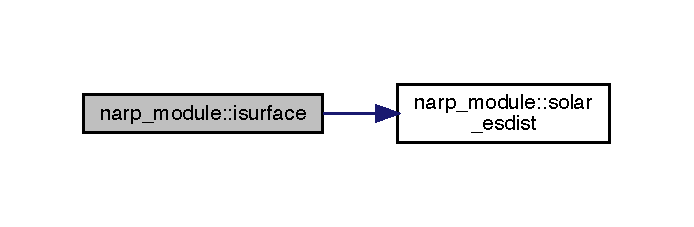
\includegraphics[width=333pt]{namespacenarp__module_a67c38c5ffd466f983c36961a978ca980_cgraph}
\end{center}
\end{figure}
\mbox{\Hypertarget{namespacenarp__module_ac480c3115a6413b9e79770f601e68895}\label{namespacenarp__module_ac480c3115a6413b9e79770f601e68895}} 
\index{narp\+\_\+module@{narp\+\_\+module}!narp@{narp}}
\index{narp@{narp}!narp\+\_\+module@{narp\+\_\+module}}
\subsubsection{\texorpdfstring{narp()}{narp()}}
{\footnotesize\ttfamily subroutine narp\+\_\+module\+::narp (\begin{DoxyParamCaption}\item[{real(kind(1d0)), intent(in)}]{D\+T\+I\+ME,  }\item[{real(kind(1d0)), intent(in)}]{Z\+E\+N\+I\+T\+H\+\_\+deg,  }\item[{real(kind(1d0)), intent(in)}]{kdown,  }\item[{real(kind(1d0)), intent(in)}]{Temp\+\_\+C,  }\item[{real(kind(1d0)), intent(in)}]{RH,  }\item[{real(kind(1d0)), intent(in)}]{Press\+\_\+h\+Pa,  }\item[{real(kind(1d0)), intent(in)}]{qn1\+\_\+obs,  }\item[{real(kind(1d0)), intent(in)}]{Snow\+Alb,  }\item[{integer, intent(in)}]{Albedo\+Choice,  }\item[{integer, intent(in)}]{ldown\+\_\+option,  }\item[{integer, intent(in)}]{Net\+Radiation\+Method,  }\item[{integer, intent(in)}]{Diag\+QN,  }\item[{real(kind(1d0)), intent(out)}]{Q\+S\+T\+A\+Rall,  }\item[{real(kind(1d0)), intent(out)}]{Q\+S\+T\+A\+R\+\_\+\+SF,  }\item[{real(kind(1d0)), intent(out)}]{Q\+S\+T\+A\+R\+\_\+S,  }\item[{real(kind(1d0)), intent(out)}]{kclear,  }\item[{real(kind(1d0)), intent(out)}]{K\+U\+Pall,  }\item[{real(kind(1d0)), intent(out)}]{L\+Down,  }\item[{real(kind(1d0)), intent(out)}]{L\+U\+Pall,  }\item[{real(kind(1d0)), intent(out)}]{fcld,  }\item[{real(kind(1d0)), intent(out)}]{T\+S\+U\+R\+Fall }\end{DoxyParamCaption})}



Definition at line 51 of file L\+U\+M\+P\+S\+\_\+\+N\+A\+R\+P\+\_\+v3.\+f95.

Here is the call graph for this function\+:\nopagebreak
\begin{figure}[H]
\begin{center}
\leavevmode
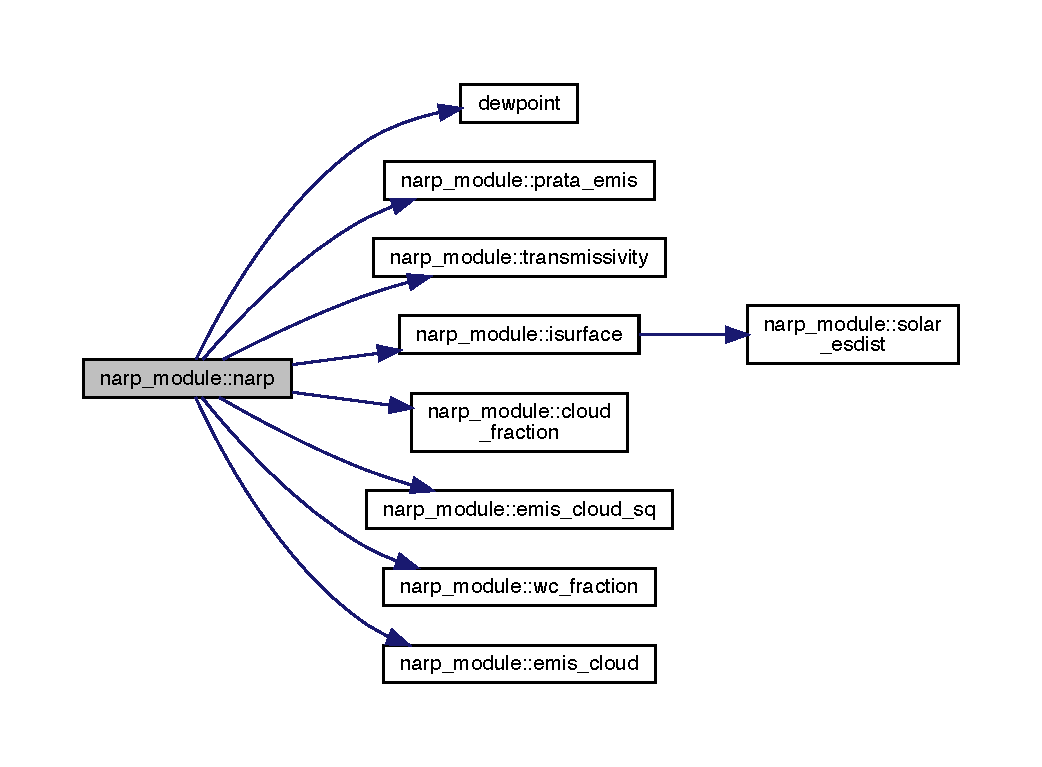
\includegraphics[width=350pt]{namespacenarp__module_ac480c3115a6413b9e79770f601e68895_cgraph}
\end{center}
\end{figure}
\mbox{\Hypertarget{namespacenarp__module_acfe7f0cf64c053bc528f54bde3ce8194}\label{namespacenarp__module_acfe7f0cf64c053bc528f54bde3ce8194}} 
\index{narp\+\_\+module@{narp\+\_\+module}!prata\+\_\+emis@{prata\+\_\+emis}}
\index{prata\+\_\+emis@{prata\+\_\+emis}!narp\+\_\+module@{narp\+\_\+module}}
\subsubsection{\texorpdfstring{prata\+\_\+emis()}{prata\_emis()}}
{\footnotesize\ttfamily real(kind(1d0)) function narp\+\_\+module\+::prata\+\_\+emis (\begin{DoxyParamCaption}\item[{real(kind(1d0))}]{Temp\+\_\+K,  }\item[{real(kind(1d0))}]{E\+A\+\_\+h\+Pa }\end{DoxyParamCaption})}



Definition at line 335 of file L\+U\+M\+P\+S\+\_\+\+N\+A\+R\+P\+\_\+v3.\+f95.

\mbox{\Hypertarget{namespacenarp__module_a2855b93202c40f690a05a6febcdc8067}\label{namespacenarp__module_a2855b93202c40f690a05a6febcdc8067}} 
\index{narp\+\_\+module@{narp\+\_\+module}!smithlambda@{smithlambda}}
\index{smithlambda@{smithlambda}!narp\+\_\+module@{narp\+\_\+module}}
\subsubsection{\texorpdfstring{smithlambda()}{smithlambda()}}
{\footnotesize\ttfamily real(kind(1d0)) function, dimension(365) narp\+\_\+module\+::smithlambda (\begin{DoxyParamCaption}\item[{integer}]{lat }\end{DoxyParamCaption})}



Definition at line 446 of file L\+U\+M\+P\+S\+\_\+\+N\+A\+R\+P\+\_\+v3.\+f95.

Here is the call graph for this function\+:\nopagebreak
\begin{figure}[H]
\begin{center}
\leavevmode
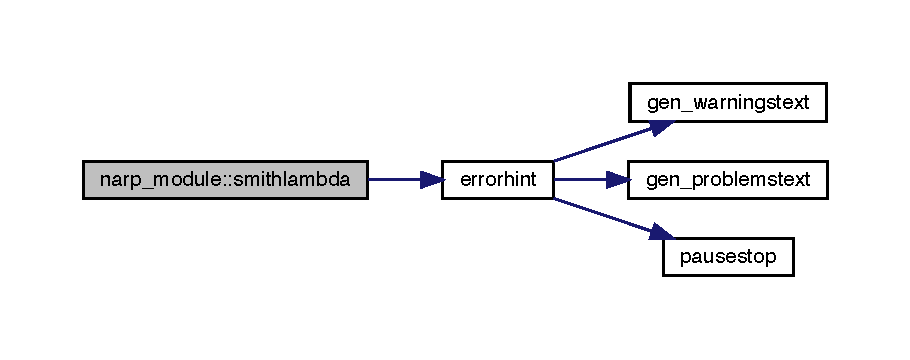
\includegraphics[width=350pt]{namespacenarp__module_a2855b93202c40f690a05a6febcdc8067_cgraph}
\end{center}
\end{figure}
\mbox{\Hypertarget{namespacenarp__module_ada3ea94f7e9dc6f9fc5bc22c4b1d8a68}\label{namespacenarp__module_ada3ea94f7e9dc6f9fc5bc22c4b1d8a68}} 
\index{narp\+\_\+module@{narp\+\_\+module}!solar\+\_\+esdist@{solar\+\_\+esdist}}
\index{solar\+\_\+esdist@{solar\+\_\+esdist}!narp\+\_\+module@{narp\+\_\+module}}
\subsubsection{\texorpdfstring{solar\+\_\+esdist()}{solar\_esdist()}}
{\footnotesize\ttfamily real(kind(1d0)) function narp\+\_\+module\+::solar\+\_\+esdist (\begin{DoxyParamCaption}\item[{integer}]{doy }\end{DoxyParamCaption})}



Definition at line 430 of file L\+U\+M\+P\+S\+\_\+\+N\+A\+R\+P\+\_\+v3.\+f95.

\mbox{\Hypertarget{namespacenarp__module_aeae3a1e345682a38338ecdf71bcf1c8e}\label{namespacenarp__module_aeae3a1e345682a38338ecdf71bcf1c8e}} 
\index{narp\+\_\+module@{narp\+\_\+module}!transmissivity@{transmissivity}}
\index{transmissivity@{transmissivity}!narp\+\_\+module@{narp\+\_\+module}}
\subsubsection{\texorpdfstring{transmissivity()}{transmissivity()}}
{\footnotesize\ttfamily real(kind(1d0)) function narp\+\_\+module\+::transmissivity (\begin{DoxyParamCaption}\item[{real(kind(1d0))}]{Press\+\_\+h\+Pa,  }\item[{real(kind(1d0))}]{Temp\+\_\+\+C\+\_\+dew,  }\item[{real(kind(1d0))}]{G,  }\item[{real(kind(1d0))}]{zenith }\end{DoxyParamCaption})}



Definition at line 467 of file L\+U\+M\+P\+S\+\_\+\+N\+A\+R\+P\+\_\+v3.\+f95.

\mbox{\Hypertarget{namespacenarp__module_a1774d32db350c89aad964f2f45ceb46e}\label{namespacenarp__module_a1774d32db350c89aad964f2f45ceb46e}} 
\index{narp\+\_\+module@{narp\+\_\+module}!wc\+\_\+fraction@{wc\+\_\+fraction}}
\index{wc\+\_\+fraction@{wc\+\_\+fraction}!narp\+\_\+module@{narp\+\_\+module}}
\subsubsection{\texorpdfstring{wc\+\_\+fraction()}{wc\_fraction()}}
{\footnotesize\ttfamily real(kind(1d0)) function narp\+\_\+module\+::wc\+\_\+fraction (\begin{DoxyParamCaption}\item[{real(kind(1d0)), intent(in)}]{RH,  }\item[{real(kind(1d0)), intent(in)}]{Temp }\end{DoxyParamCaption})}



Definition at line 366 of file L\+U\+M\+P\+S\+\_\+\+N\+A\+R\+P\+\_\+v3.\+f95.


\hypertarget{namespacephysconstants}{}\section{physconstants Module Reference}
\label{namespacephysconstants}\index{physconstants@{physconstants}}
\subsection*{Variables}
\begin{DoxyCompactItemize}
\item 
real(kind(1d0)), parameter \hyperlink{namespacephysconstants_a3440be0c8f808e005a3f8400ebe8ea07}{c2k} = 273.\+15
\item 
real(kind(1d0)), parameter \hyperlink{namespacephysconstants_ace6c4e6b3043559bb2ee21b5f4c2cc8e}{sbconst} = 5.\+67051e-\/8
\item 
real(kind(1d0)), parameter \hyperlink{namespacephysconstants_a73315ec4406d89b720497281c9353eb2}{jtoumolpar} = 4.\+6
\end{DoxyCompactItemize}


\subsection{Variable Documentation}
\mbox{\Hypertarget{namespacephysconstants_a3440be0c8f808e005a3f8400ebe8ea07}\label{namespacephysconstants_a3440be0c8f808e005a3f8400ebe8ea07}} 
\index{physconstants@{physconstants}!c2k@{c2k}}
\index{c2k@{c2k}!physconstants@{physconstants}}
\subsubsection{\texorpdfstring{c2k}{c2k}}
{\footnotesize\ttfamily real (kind(1d0)), parameter physconstants\+::c2k = 273.\+15}



Definition at line 2117 of file L\+U\+M\+P\+S\+\_\+\+Module\+\_\+constants.\+f95.

\mbox{\Hypertarget{namespacephysconstants_a73315ec4406d89b720497281c9353eb2}\label{namespacephysconstants_a73315ec4406d89b720497281c9353eb2}} 
\index{physconstants@{physconstants}!jtoumolpar@{jtoumolpar}}
\index{jtoumolpar@{jtoumolpar}!physconstants@{physconstants}}
\subsubsection{\texorpdfstring{jtoumolpar}{jtoumolpar}}
{\footnotesize\ttfamily real (kind(1d0)), parameter physconstants\+::jtoumolpar = 4.\+6}



Definition at line 2119 of file L\+U\+M\+P\+S\+\_\+\+Module\+\_\+constants.\+f95.

\mbox{\Hypertarget{namespacephysconstants_ace6c4e6b3043559bb2ee21b5f4c2cc8e}\label{namespacephysconstants_ace6c4e6b3043559bb2ee21b5f4c2cc8e}} 
\index{physconstants@{physconstants}!sbconst@{sbconst}}
\index{sbconst@{sbconst}!physconstants@{physconstants}}
\subsubsection{\texorpdfstring{sbconst}{sbconst}}
{\footnotesize\ttfamily real (kind(1d0)), parameter physconstants\+::sbconst = 5.\+67051e-\/8}



Definition at line 2118 of file L\+U\+M\+P\+S\+\_\+\+Module\+\_\+constants.\+f95.


\hypertarget{namespaceprecision}{}\section{precision Module Reference}
\label{namespaceprecision}\index{precision@{precision}}
\subsection*{Variables}
\begin{DoxyCompactItemize}
\item 
integer, parameter \hyperlink{namespaceprecision_ae184f50eb0c9c763233e9c5d34b8034a}{kr4} = selected\+\_\+real\+\_\+kind(6, 37)
\item 
integer, parameter \hyperlink{namespaceprecision_a4b30cd5919aba1303b7b752110b57254}{kr8} = selected\+\_\+real\+\_\+kind(15, 307)
\item 
integer, parameter \hyperlink{namespaceprecision_a7b97657c46b1524ed5f73ffc1226dc08}{ki4} = selected\+\_\+int\+\_\+kind(9)
\item 
integer, parameter \hyperlink{namespaceprecision_a25d156062c1ee160ed75a5a6dced7ceb}{ki8} = selected\+\_\+int\+\_\+kind(18)
\item 
integer, parameter \hyperlink{namespaceprecision_a6a58f4fab509ea84cc60d30e25bcb1ca}{kc4} = \hyperlink{namespaceprecision_ae184f50eb0c9c763233e9c5d34b8034a}{kr4}
\item 
integer, parameter \hyperlink{namespaceprecision_a2093064d9b44820731402869509b1a0d}{kc8} = \hyperlink{namespaceprecision_a4b30cd5919aba1303b7b752110b57254}{kr8}
\end{DoxyCompactItemize}


\subsection{Variable Documentation}
\mbox{\Hypertarget{namespaceprecision_a6a58f4fab509ea84cc60d30e25bcb1ca}\label{namespaceprecision_a6a58f4fab509ea84cc60d30e25bcb1ca}} 
\index{precision@{precision}!kc4@{kc4}}
\index{kc4@{kc4}!precision@{precision}}
\subsubsection{\texorpdfstring{kc4}{kc4}}
{\footnotesize\ttfamily integer, parameter precision\+::kc4 = \hyperlink{namespaceprecision_ae184f50eb0c9c763233e9c5d34b8034a}{kr4}}



Definition at line 16 of file precmod.\+f95.

\mbox{\Hypertarget{namespaceprecision_a2093064d9b44820731402869509b1a0d}\label{namespaceprecision_a2093064d9b44820731402869509b1a0d}} 
\index{precision@{precision}!kc8@{kc8}}
\index{kc8@{kc8}!precision@{precision}}
\subsubsection{\texorpdfstring{kc8}{kc8}}
{\footnotesize\ttfamily integer, parameter precision\+::kc8 = \hyperlink{namespaceprecision_a4b30cd5919aba1303b7b752110b57254}{kr8}}



Definition at line 17 of file precmod.\+f95.

\mbox{\Hypertarget{namespaceprecision_a7b97657c46b1524ed5f73ffc1226dc08}\label{namespaceprecision_a7b97657c46b1524ed5f73ffc1226dc08}} 
\index{precision@{precision}!ki4@{ki4}}
\index{ki4@{ki4}!precision@{precision}}
\subsubsection{\texorpdfstring{ki4}{ki4}}
{\footnotesize\ttfamily integer, parameter precision\+::ki4 = selected\+\_\+int\+\_\+kind(9)}



Definition at line 11 of file precmod.\+f95.

\mbox{\Hypertarget{namespaceprecision_a25d156062c1ee160ed75a5a6dced7ceb}\label{namespaceprecision_a25d156062c1ee160ed75a5a6dced7ceb}} 
\index{precision@{precision}!ki8@{ki8}}
\index{ki8@{ki8}!precision@{precision}}
\subsubsection{\texorpdfstring{ki8}{ki8}}
{\footnotesize\ttfamily integer, parameter precision\+::ki8 = selected\+\_\+int\+\_\+kind(18)}



Definition at line 12 of file precmod.\+f95.

\mbox{\Hypertarget{namespaceprecision_ae184f50eb0c9c763233e9c5d34b8034a}\label{namespaceprecision_ae184f50eb0c9c763233e9c5d34b8034a}} 
\index{precision@{precision}!kr4@{kr4}}
\index{kr4@{kr4}!precision@{precision}}
\subsubsection{\texorpdfstring{kr4}{kr4}}
{\footnotesize\ttfamily integer, parameter precision\+::kr4 = selected\+\_\+real\+\_\+kind(6, 37)}



Definition at line 6 of file precmod.\+f95.

\mbox{\Hypertarget{namespaceprecision_a4b30cd5919aba1303b7b752110b57254}\label{namespaceprecision_a4b30cd5919aba1303b7b752110b57254}} 
\index{precision@{precision}!kr8@{kr8}}
\index{kr8@{kr8}!precision@{precision}}
\subsubsection{\texorpdfstring{kr8}{kr8}}
{\footnotesize\ttfamily integer, parameter precision\+::kr8 = selected\+\_\+real\+\_\+kind(15, 307)}



Definition at line 7 of file precmod.\+f95.


\hypertarget{namespaceqsort__c__module}{}\section{qsort\+\_\+c\+\_\+module Module Reference}
\label{namespaceqsort__c__module}\index{qsort\+\_\+c\+\_\+module@{qsort\+\_\+c\+\_\+module}}
\subsection*{Functions/\+Subroutines}
\begin{DoxyCompactItemize}
\item 
recursive subroutine, public \hyperlink{namespaceqsort__c__module_a7e39c2068ea2fa39ea9aa0d7757ceb58}{qsortc} (A)
\end{DoxyCompactItemize}


\subsection{Function/\+Subroutine Documentation}
\mbox{\Hypertarget{namespaceqsort__c__module_a7e39c2068ea2fa39ea9aa0d7757ceb58}\label{namespaceqsort__c__module_a7e39c2068ea2fa39ea9aa0d7757ceb58}} 
\index{qsort\+\_\+c\+\_\+module@{qsort\+\_\+c\+\_\+module}!qsortc@{qsortc}}
\index{qsortc@{qsortc}!qsort\+\_\+c\+\_\+module@{qsort\+\_\+c\+\_\+module}}
\subsubsection{\texorpdfstring{qsortc()}{qsortc()}}
{\footnotesize\ttfamily recursive subroutine, public qsort\+\_\+c\+\_\+module\+::qsortc (\begin{DoxyParamCaption}\item[{real, dimension(\+:), intent(inout)}]{A }\end{DoxyParamCaption})}



Definition at line 19 of file qsort\+\_\+c\+\_\+module.\+f95.


\hypertarget{namespaceresist}{}\section{resist Module Reference}
\label{namespaceresist}\index{resist@{resist}}
\subsection*{Variables}
\begin{DoxyCompactItemize}
\item 
real(kind(1d0)) \hyperlink{namespaceresist_a4a4f565342a527412998f585a5c126be}{th}
\item 
real(kind(1d0)) \hyperlink{namespaceresist_ac5a785e8c6079704fe779baff78c5c54}{tl}
\item 
real(kind(1d0)) \hyperlink{namespaceresist_ab582d1ab5eac071afaba0e8b351311ff}{kmax}
\item 
real(kind(1d0)) \hyperlink{namespaceresist_a55e0021876c70be1f609dc187f92f705}{g1}
\item 
real(kind(1d0)) \hyperlink{namespaceresist_a98bae857808870e126fd947cdb3b9b14}{g2}
\item 
real(kind(1d0)) \hyperlink{namespaceresist_a35b3f7080e2cc3d5883dbd59f8cfb21b}{g3}
\item 
real(kind(1d0)) \hyperlink{namespaceresist_a9d34a5c68ab32cd207e570225330120b}{g4}
\item 
real(kind(1d0)) \hyperlink{namespaceresist_aca3b131857592b71ec28cce48a2fb0ee}{g5}
\item 
real(kind(1d0)) \hyperlink{namespaceresist_a7ad9926600ac79377439521a837b21de}{g6}
\item 
real(kind(1d0)) \hyperlink{namespaceresist_a8ce25344e41b31f4da68572adc0b8391}{s1}
\item 
real(kind(1d0)) \hyperlink{namespaceresist_a0edd3d2ed03de65fa65ffe839661d97c}{s2}
\item 
real(kind(1d0)) \hyperlink{namespaceresist_a018715832aa4e47e3fd4deb59e413da1}{tc}
\item 
real(kind(1d0)) \hyperlink{namespaceresist_a39c5aa18f024567bd7365dbdfe6c7216}{tc2}
\item 
integer \hyperlink{namespaceresist_a89895984ab23ef2627cb851eadd8b858}{gsmodel}
\end{DoxyCompactItemize}


\subsection{Variable Documentation}
\mbox{\Hypertarget{namespaceresist_a55e0021876c70be1f609dc187f92f705}\label{namespaceresist_a55e0021876c70be1f609dc187f92f705}} 
\index{resist@{resist}!g1@{g1}}
\index{g1@{g1}!resist@{resist}}
\subsubsection{\texorpdfstring{g1}{g1}}
{\footnotesize\ttfamily real (kind(1d0)) resist\+::g1}



Definition at line 1208 of file L\+U\+M\+P\+S\+\_\+\+Module\+\_\+constants.\+f95.

\mbox{\Hypertarget{namespaceresist_a98bae857808870e126fd947cdb3b9b14}\label{namespaceresist_a98bae857808870e126fd947cdb3b9b14}} 
\index{resist@{resist}!g2@{g2}}
\index{g2@{g2}!resist@{resist}}
\subsubsection{\texorpdfstring{g2}{g2}}
{\footnotesize\ttfamily real (kind(1d0)) resist\+::g2}



Definition at line 1208 of file L\+U\+M\+P\+S\+\_\+\+Module\+\_\+constants.\+f95.

\mbox{\Hypertarget{namespaceresist_a35b3f7080e2cc3d5883dbd59f8cfb21b}\label{namespaceresist_a35b3f7080e2cc3d5883dbd59f8cfb21b}} 
\index{resist@{resist}!g3@{g3}}
\index{g3@{g3}!resist@{resist}}
\subsubsection{\texorpdfstring{g3}{g3}}
{\footnotesize\ttfamily real (kind(1d0)) resist\+::g3}



Definition at line 1208 of file L\+U\+M\+P\+S\+\_\+\+Module\+\_\+constants.\+f95.

\mbox{\Hypertarget{namespaceresist_a9d34a5c68ab32cd207e570225330120b}\label{namespaceresist_a9d34a5c68ab32cd207e570225330120b}} 
\index{resist@{resist}!g4@{g4}}
\index{g4@{g4}!resist@{resist}}
\subsubsection{\texorpdfstring{g4}{g4}}
{\footnotesize\ttfamily real (kind(1d0)) resist\+::g4}



Definition at line 1208 of file L\+U\+M\+P\+S\+\_\+\+Module\+\_\+constants.\+f95.

\mbox{\Hypertarget{namespaceresist_aca3b131857592b71ec28cce48a2fb0ee}\label{namespaceresist_aca3b131857592b71ec28cce48a2fb0ee}} 
\index{resist@{resist}!g5@{g5}}
\index{g5@{g5}!resist@{resist}}
\subsubsection{\texorpdfstring{g5}{g5}}
{\footnotesize\ttfamily real (kind(1d0)) resist\+::g5}



Definition at line 1208 of file L\+U\+M\+P\+S\+\_\+\+Module\+\_\+constants.\+f95.

\mbox{\Hypertarget{namespaceresist_a7ad9926600ac79377439521a837b21de}\label{namespaceresist_a7ad9926600ac79377439521a837b21de}} 
\index{resist@{resist}!g6@{g6}}
\index{g6@{g6}!resist@{resist}}
\subsubsection{\texorpdfstring{g6}{g6}}
{\footnotesize\ttfamily real (kind(1d0)) resist\+::g6}



Definition at line 1208 of file L\+U\+M\+P\+S\+\_\+\+Module\+\_\+constants.\+f95.

\mbox{\Hypertarget{namespaceresist_a89895984ab23ef2627cb851eadd8b858}\label{namespaceresist_a89895984ab23ef2627cb851eadd8b858}} 
\index{resist@{resist}!gsmodel@{gsmodel}}
\index{gsmodel@{gsmodel}!resist@{resist}}
\subsubsection{\texorpdfstring{gsmodel}{gsmodel}}
{\footnotesize\ttfamily integer resist\+::gsmodel}



Definition at line 1215 of file L\+U\+M\+P\+S\+\_\+\+Module\+\_\+constants.\+f95.

\mbox{\Hypertarget{namespaceresist_ab582d1ab5eac071afaba0e8b351311ff}\label{namespaceresist_ab582d1ab5eac071afaba0e8b351311ff}} 
\index{resist@{resist}!kmax@{kmax}}
\index{kmax@{kmax}!resist@{resist}}
\subsubsection{\texorpdfstring{kmax}{kmax}}
{\footnotesize\ttfamily real (kind(1d0)) resist\+::kmax}



Definition at line 1208 of file L\+U\+M\+P\+S\+\_\+\+Module\+\_\+constants.\+f95.

\mbox{\Hypertarget{namespaceresist_a8ce25344e41b31f4da68572adc0b8391}\label{namespaceresist_a8ce25344e41b31f4da68572adc0b8391}} 
\index{resist@{resist}!s1@{s1}}
\index{s1@{s1}!resist@{resist}}
\subsubsection{\texorpdfstring{s1}{s1}}
{\footnotesize\ttfamily real (kind(1d0)) resist\+::s1}



Definition at line 1208 of file L\+U\+M\+P\+S\+\_\+\+Module\+\_\+constants.\+f95.

\mbox{\Hypertarget{namespaceresist_a0edd3d2ed03de65fa65ffe839661d97c}\label{namespaceresist_a0edd3d2ed03de65fa65ffe839661d97c}} 
\index{resist@{resist}!s2@{s2}}
\index{s2@{s2}!resist@{resist}}
\subsubsection{\texorpdfstring{s2}{s2}}
{\footnotesize\ttfamily real (kind(1d0)) resist\+::s2}



Definition at line 1208 of file L\+U\+M\+P\+S\+\_\+\+Module\+\_\+constants.\+f95.

\mbox{\Hypertarget{namespaceresist_a018715832aa4e47e3fd4deb59e413da1}\label{namespaceresist_a018715832aa4e47e3fd4deb59e413da1}} 
\index{resist@{resist}!tc@{tc}}
\index{tc@{tc}!resist@{resist}}
\subsubsection{\texorpdfstring{tc}{tc}}
{\footnotesize\ttfamily real (kind(1d0)) resist\+::tc}



Definition at line 1208 of file L\+U\+M\+P\+S\+\_\+\+Module\+\_\+constants.\+f95.

\mbox{\Hypertarget{namespaceresist_a39c5aa18f024567bd7365dbdfe6c7216}\label{namespaceresist_a39c5aa18f024567bd7365dbdfe6c7216}} 
\index{resist@{resist}!tc2@{tc2}}
\index{tc2@{tc2}!resist@{resist}}
\subsubsection{\texorpdfstring{tc2}{tc2}}
{\footnotesize\ttfamily real (kind(1d0)) resist\+::tc2}



Definition at line 1208 of file L\+U\+M\+P\+S\+\_\+\+Module\+\_\+constants.\+f95.

\mbox{\Hypertarget{namespaceresist_a4a4f565342a527412998f585a5c126be}\label{namespaceresist_a4a4f565342a527412998f585a5c126be}} 
\index{resist@{resist}!th@{th}}
\index{th@{th}!resist@{resist}}
\subsubsection{\texorpdfstring{th}{th}}
{\footnotesize\ttfamily real (kind(1d0)) resist\+::th}



Definition at line 1208 of file L\+U\+M\+P\+S\+\_\+\+Module\+\_\+constants.\+f95.

\mbox{\Hypertarget{namespaceresist_ac5a785e8c6079704fe779baff78c5c54}\label{namespaceresist_ac5a785e8c6079704fe779baff78c5c54}} 
\index{resist@{resist}!tl@{tl}}
\index{tl@{tl}!resist@{resist}}
\subsubsection{\texorpdfstring{tl}{tl}}
{\footnotesize\ttfamily real (kind(1d0)) resist\+::tl}



Definition at line 1208 of file L\+U\+M\+P\+S\+\_\+\+Module\+\_\+constants.\+f95.


\hypertarget{namespacerun__info}{}\section{run\+\_\+info Module Reference}
\label{namespacerun__info}\index{run\+\_\+info@{run\+\_\+info}}
\subsection*{Variables}
\begin{DoxyCompactItemize}
\item 
character(len=90), dimension(14) \hyperlink{namespacerun__info_a7ebcc0191b287ed4b8f80e6080cc1dc8}{text}
\item 
integer \hyperlink{namespacerun__info_a4406caf0abae1b67ad05c7ed0c7904c0}{lim0} =0
\item 
integer \hyperlink{namespacerun__info_adc3a55251266df823d3449b67005bade}{lim1} =1
\item 
integer \hyperlink{namespacerun__info_af89da03470d913f288c8deaa72c81e98}{lim2} =2
\item 
integer \hyperlink{namespacerun__info_a776a112d5d931e6d58195aac621d98c8}{lim4} =4
\item 
integer \hyperlink{namespacerun__info_ad7a71d5b6da02d9fe343cf50247e63f1}{lim3} =3
\item 
integer \hyperlink{namespacerun__info_a30737240d73cc13facaa16e6234df127}{lim6} =6
\item 
integer \hyperlink{namespacerun__info_a541da993ba7c0323fde4a512605bbe8f}{lim8} =8
\item 
integer \hyperlink{namespacerun__info_a635c9fcab621a64612a513a423762d84}{lim12} =12
\item 
integer \hyperlink{namespacerun__info_ab21dc24ae87c9094754723447a6c94e5}{lfn\+\_\+us}
\item 
logical \hyperlink{namespacerun__info_a0ccca59a580a8242d13b9e96cc6d1d4d}{file\+\_\+qs}
\end{DoxyCompactItemize}


\subsection{Variable Documentation}
\mbox{\Hypertarget{namespacerun__info_a0ccca59a580a8242d13b9e96cc6d1d4d}\label{namespacerun__info_a0ccca59a580a8242d13b9e96cc6d1d4d}} 
\index{run\+\_\+info@{run\+\_\+info}!file\+\_\+qs@{file\+\_\+qs}}
\index{file\+\_\+qs@{file\+\_\+qs}!run\+\_\+info@{run\+\_\+info}}
\subsubsection{\texorpdfstring{file\+\_\+qs}{file\_qs}}
{\footnotesize\ttfamily logical run\+\_\+info\+::file\+\_\+qs}



Definition at line 13 of file S\+U\+E\+W\+S\+\_\+\+Files\+\_\+run\+\_\+\+Control.\+f95.

\mbox{\Hypertarget{namespacerun__info_ab21dc24ae87c9094754723447a6c94e5}\label{namespacerun__info_ab21dc24ae87c9094754723447a6c94e5}} 
\index{run\+\_\+info@{run\+\_\+info}!lfn\+\_\+us@{lfn\+\_\+us}}
\index{lfn\+\_\+us@{lfn\+\_\+us}!run\+\_\+info@{run\+\_\+info}}
\subsubsection{\texorpdfstring{lfn\+\_\+us}{lfn\_us}}
{\footnotesize\ttfamily integer run\+\_\+info\+::lfn\+\_\+us}



Definition at line 12 of file S\+U\+E\+W\+S\+\_\+\+Files\+\_\+run\+\_\+\+Control.\+f95.

\mbox{\Hypertarget{namespacerun__info_a4406caf0abae1b67ad05c7ed0c7904c0}\label{namespacerun__info_a4406caf0abae1b67ad05c7ed0c7904c0}} 
\index{run\+\_\+info@{run\+\_\+info}!lim0@{lim0}}
\index{lim0@{lim0}!run\+\_\+info@{run\+\_\+info}}
\subsubsection{\texorpdfstring{lim0}{lim0}}
{\footnotesize\ttfamily integer run\+\_\+info\+::lim0 =0}



Definition at line 12 of file S\+U\+E\+W\+S\+\_\+\+Files\+\_\+run\+\_\+\+Control.\+f95.

\mbox{\Hypertarget{namespacerun__info_adc3a55251266df823d3449b67005bade}\label{namespacerun__info_adc3a55251266df823d3449b67005bade}} 
\index{run\+\_\+info@{run\+\_\+info}!lim1@{lim1}}
\index{lim1@{lim1}!run\+\_\+info@{run\+\_\+info}}
\subsubsection{\texorpdfstring{lim1}{lim1}}
{\footnotesize\ttfamily integer run\+\_\+info\+::lim1 =1}



Definition at line 12 of file S\+U\+E\+W\+S\+\_\+\+Files\+\_\+run\+\_\+\+Control.\+f95.

\mbox{\Hypertarget{namespacerun__info_a635c9fcab621a64612a513a423762d84}\label{namespacerun__info_a635c9fcab621a64612a513a423762d84}} 
\index{run\+\_\+info@{run\+\_\+info}!lim12@{lim12}}
\index{lim12@{lim12}!run\+\_\+info@{run\+\_\+info}}
\subsubsection{\texorpdfstring{lim12}{lim12}}
{\footnotesize\ttfamily integer run\+\_\+info\+::lim12 =12}



Definition at line 12 of file S\+U\+E\+W\+S\+\_\+\+Files\+\_\+run\+\_\+\+Control.\+f95.

\mbox{\Hypertarget{namespacerun__info_af89da03470d913f288c8deaa72c81e98}\label{namespacerun__info_af89da03470d913f288c8deaa72c81e98}} 
\index{run\+\_\+info@{run\+\_\+info}!lim2@{lim2}}
\index{lim2@{lim2}!run\+\_\+info@{run\+\_\+info}}
\subsubsection{\texorpdfstring{lim2}{lim2}}
{\footnotesize\ttfamily integer run\+\_\+info\+::lim2 =2}



Definition at line 12 of file S\+U\+E\+W\+S\+\_\+\+Files\+\_\+run\+\_\+\+Control.\+f95.

\mbox{\Hypertarget{namespacerun__info_ad7a71d5b6da02d9fe343cf50247e63f1}\label{namespacerun__info_ad7a71d5b6da02d9fe343cf50247e63f1}} 
\index{run\+\_\+info@{run\+\_\+info}!lim3@{lim3}}
\index{lim3@{lim3}!run\+\_\+info@{run\+\_\+info}}
\subsubsection{\texorpdfstring{lim3}{lim3}}
{\footnotesize\ttfamily integer run\+\_\+info\+::lim3 =3}



Definition at line 12 of file S\+U\+E\+W\+S\+\_\+\+Files\+\_\+run\+\_\+\+Control.\+f95.

\mbox{\Hypertarget{namespacerun__info_a776a112d5d931e6d58195aac621d98c8}\label{namespacerun__info_a776a112d5d931e6d58195aac621d98c8}} 
\index{run\+\_\+info@{run\+\_\+info}!lim4@{lim4}}
\index{lim4@{lim4}!run\+\_\+info@{run\+\_\+info}}
\subsubsection{\texorpdfstring{lim4}{lim4}}
{\footnotesize\ttfamily integer run\+\_\+info\+::lim4 =4}



Definition at line 12 of file S\+U\+E\+W\+S\+\_\+\+Files\+\_\+run\+\_\+\+Control.\+f95.

\mbox{\Hypertarget{namespacerun__info_a30737240d73cc13facaa16e6234df127}\label{namespacerun__info_a30737240d73cc13facaa16e6234df127}} 
\index{run\+\_\+info@{run\+\_\+info}!lim6@{lim6}}
\index{lim6@{lim6}!run\+\_\+info@{run\+\_\+info}}
\subsubsection{\texorpdfstring{lim6}{lim6}}
{\footnotesize\ttfamily integer run\+\_\+info\+::lim6 =6}



Definition at line 12 of file S\+U\+E\+W\+S\+\_\+\+Files\+\_\+run\+\_\+\+Control.\+f95.

\mbox{\Hypertarget{namespacerun__info_a541da993ba7c0323fde4a512605bbe8f}\label{namespacerun__info_a541da993ba7c0323fde4a512605bbe8f}} 
\index{run\+\_\+info@{run\+\_\+info}!lim8@{lim8}}
\index{lim8@{lim8}!run\+\_\+info@{run\+\_\+info}}
\subsubsection{\texorpdfstring{lim8}{lim8}}
{\footnotesize\ttfamily integer run\+\_\+info\+::lim8 =8}



Definition at line 12 of file S\+U\+E\+W\+S\+\_\+\+Files\+\_\+run\+\_\+\+Control.\+f95.

\mbox{\Hypertarget{namespacerun__info_a7ebcc0191b287ed4b8f80e6080cc1dc8}\label{namespacerun__info_a7ebcc0191b287ed4b8f80e6080cc1dc8}} 
\index{run\+\_\+info@{run\+\_\+info}!text@{text}}
\index{text@{text}!run\+\_\+info@{run\+\_\+info}}
\subsubsection{\texorpdfstring{text}{text}}
{\footnotesize\ttfamily character (len=90), dimension(14) run\+\_\+info\+::text}



Definition at line 11 of file S\+U\+E\+W\+S\+\_\+\+Files\+\_\+run\+\_\+\+Control.\+f95.


\hypertarget{namespacesnowmod}{}\section{snowmod Module Reference}
\label{namespacesnowmod}\index{snowmod@{snowmod}}
\subsection*{Variables}
\begin{DoxyCompactItemize}
\item 
real(kind(1d0)) \hyperlink{namespacesnowmod_a5c337bba47f88549ed03afb42d5d097d}{adjmeltfact}
\item 
real(kind(1d0)) \hyperlink{namespacesnowmod_a78e0393f653cfdebf0ccab83abc0b800}{cumsnowfall}
\item 
real(kind(1d0)) \hyperlink{namespacesnowmod_a67018a3202a62ad0d4e7715dbfcf5e50}{fwh}
\item 
real(kind(1d0)) \hyperlink{namespacesnowmod_aa988f82274f056c6d2f7ed3d37457b24}{lvs\+\_\+j\+\_\+kg}
\item 
real(kind(1d0)) \hyperlink{namespacesnowmod_a7e8123e5b32bedfb676ea5c6ca62272a}{mwh}
\item 
real(kind(1d0)) \hyperlink{namespacesnowmod_affe56e4e5f1d5df5d7f4bbae7ae22541}{mwstore}
\item 
real(kind(1d0)) \hyperlink{namespacesnowmod_a9e24791cb966600bc8e20739bc1f36b3}{preciplimit}
\item 
real(kind(1d0)) \hyperlink{namespacesnowmod_a5dcda7794eeea3753a3f14cd6fdf47b8}{preciplimitalb}
\item 
real(kind(1d0)) \hyperlink{namespacesnowmod_a1d7e7d0b8974783e0320cde393e09594}{qm}
\item 
real(kind(1d0)) \hyperlink{namespacesnowmod_adbb58215814d438f2486f880958737be}{qmfreez}
\item 
real(kind(1d0)) \hyperlink{namespacesnowmod_a35fe883b6ebd9767f44c27354160afd3}{qmrain}
\item 
real(kind(1d0)) \hyperlink{namespacesnowmod_ad0e97f4f3c91c80ab519eab77750a5c0}{qn1\+\_\+snow}
\item 
real(kind(1d0)) \hyperlink{namespacesnowmod_adfca55100f9a2262f228ea1e39d61271}{qn1\+\_\+nosnow}
\item 
real(kind(1d0)) \hyperlink{namespacesnowmod_abb043edcfd004e81969e16e07ed0d646}{radmeltfact}
\item 
real(kind(1d0)) \hyperlink{namespacesnowmod_a269fc9eb4dcd8dc77888c370c046a3c2}{snowalb}
\item 
real(kind(1d0)) \hyperlink{namespacesnowmod_a96e2ce7900b7310542876993d72547ef}{snowalbmin}
\item 
real(kind(1d0)) \hyperlink{namespacesnowmod_abce33f4b342130e8ac52ef51369bc801}{snowalbmax}
\item 
real(kind(1d0)) \hyperlink{namespacesnowmod_a4b6de2a8e2186c8f314bbbfe6e78d345}{snowdensmin}
\item 
real(kind(1d0)) \hyperlink{namespacesnowmod_a8a8b8429973d4227f3f1af64ebce2e79}{snowdensmax}
\item 
real(kind(1d0)) \hyperlink{namespacesnowmod_a0462c0f187d9c6a590598f728f776991}{snowlimbuild}
\item 
real(kind(1d0)) \hyperlink{namespacesnowmod_a7e327a63642bd081c76b33340881ae7b}{snowlimpaved}
\item 
real(kind(1d0)) \hyperlink{namespacesnowmod_a216f7ed83c0474b708443eddfa6c574e}{swe}
\item 
real(kind(1d0)) \hyperlink{namespacesnowmod_a98e11e8fda25e951b1c7a65ec1d36e9f}{tau\+\_\+a}
\item 
real(kind(1d0)) \hyperlink{namespacesnowmod_adcf5755398c1385d35ef29e6f780ff9c}{tau\+\_\+f}
\item 
real(kind(1d0)) \hyperlink{namespacesnowmod_aaf08f7c00b0d87b2135341ca3f63f0d7}{tau\+\_\+r}
\item 
real(kind(1d0)) \hyperlink{namespacesnowmod_a963e4ef23aef666f3afb12096ef952b8}{tempmeltfact}
\item 
real(kind(1d0)) \hyperlink{namespacesnowmod_aef00a57fa640ad627fb60de11644e20d}{volday}
\item 
real(kind(1d0)) \hyperlink{namespacesnowmod_ab1cf232aa719c4c447ac11c210889e66}{zf}
\item 
real(kind(1d0)) \hyperlink{namespacesnowmod_a8cda7b30a924d03ee30f2bde6c9e41bc}{waterholdcapfrac}
\item 
real(kind(1d0)) \hyperlink{namespacesnowmod_ab2e9b89164bc8dd89eadb546e3ef57fa}{crwmin}
\item 
real(kind(1d0)) \hyperlink{namespacesnowmod_adec694ca0cbc2092f2c5d16238b4d0a9}{crwmax}
\item 
real(kind(1d0)), dimension(2) \hyperlink{namespacesnowmod_a9c7d574d109596d16542b38123065e66}{snowremoval} =0
\item 
real(kind(1d0)), dimension(0\+:23, 2) \hyperlink{namespacesnowmod_a1c6363fdf19c43957a62d24fa22ea25e}{snowprof}
\item 
integer \hyperlink{namespacesnowmod_afb1d5c1c466c1cb87fcf8548322581a1}{snowfractionchoice} =2
\end{DoxyCompactItemize}


\subsection{Variable Documentation}
\mbox{\Hypertarget{namespacesnowmod_a5c337bba47f88549ed03afb42d5d097d}\label{namespacesnowmod_a5c337bba47f88549ed03afb42d5d097d}} 
\index{snowmod@{snowmod}!adjmeltfact@{adjmeltfact}}
\index{adjmeltfact@{adjmeltfact}!snowmod@{snowmod}}
\subsubsection{\texorpdfstring{adjmeltfact}{adjmeltfact}}
{\footnotesize\ttfamily real (kind(1d0)) snowmod\+::adjmeltfact}



Definition at line 1096 of file L\+U\+M\+P\+S\+\_\+\+Module\+\_\+constants.\+f95.

\mbox{\Hypertarget{namespacesnowmod_adec694ca0cbc2092f2c5d16238b4d0a9}\label{namespacesnowmod_adec694ca0cbc2092f2c5d16238b4d0a9}} 
\index{snowmod@{snowmod}!crwmax@{crwmax}}
\index{crwmax@{crwmax}!snowmod@{snowmod}}
\subsubsection{\texorpdfstring{crwmax}{crwmax}}
{\footnotesize\ttfamily real (kind(1d0)) snowmod\+::crwmax}



Definition at line 1096 of file L\+U\+M\+P\+S\+\_\+\+Module\+\_\+constants.\+f95.

\mbox{\Hypertarget{namespacesnowmod_ab2e9b89164bc8dd89eadb546e3ef57fa}\label{namespacesnowmod_ab2e9b89164bc8dd89eadb546e3ef57fa}} 
\index{snowmod@{snowmod}!crwmin@{crwmin}}
\index{crwmin@{crwmin}!snowmod@{snowmod}}
\subsubsection{\texorpdfstring{crwmin}{crwmin}}
{\footnotesize\ttfamily real (kind(1d0)) snowmod\+::crwmin}



Definition at line 1096 of file L\+U\+M\+P\+S\+\_\+\+Module\+\_\+constants.\+f95.

\mbox{\Hypertarget{namespacesnowmod_a78e0393f653cfdebf0ccab83abc0b800}\label{namespacesnowmod_a78e0393f653cfdebf0ccab83abc0b800}} 
\index{snowmod@{snowmod}!cumsnowfall@{cumsnowfall}}
\index{cumsnowfall@{cumsnowfall}!snowmod@{snowmod}}
\subsubsection{\texorpdfstring{cumsnowfall}{cumsnowfall}}
{\footnotesize\ttfamily real (kind(1d0)) snowmod\+::cumsnowfall}



Definition at line 1096 of file L\+U\+M\+P\+S\+\_\+\+Module\+\_\+constants.\+f95.

\mbox{\Hypertarget{namespacesnowmod_a67018a3202a62ad0d4e7715dbfcf5e50}\label{namespacesnowmod_a67018a3202a62ad0d4e7715dbfcf5e50}} 
\index{snowmod@{snowmod}!fwh@{fwh}}
\index{fwh@{fwh}!snowmod@{snowmod}}
\subsubsection{\texorpdfstring{fwh}{fwh}}
{\footnotesize\ttfamily real (kind(1d0)) snowmod\+::fwh}



Definition at line 1096 of file L\+U\+M\+P\+S\+\_\+\+Module\+\_\+constants.\+f95.

\mbox{\Hypertarget{namespacesnowmod_aa988f82274f056c6d2f7ed3d37457b24}\label{namespacesnowmod_aa988f82274f056c6d2f7ed3d37457b24}} 
\index{snowmod@{snowmod}!lvs\+\_\+j\+\_\+kg@{lvs\+\_\+j\+\_\+kg}}
\index{lvs\+\_\+j\+\_\+kg@{lvs\+\_\+j\+\_\+kg}!snowmod@{snowmod}}
\subsubsection{\texorpdfstring{lvs\+\_\+j\+\_\+kg}{lvs\_j\_kg}}
{\footnotesize\ttfamily real (kind(1d0)) snowmod\+::lvs\+\_\+j\+\_\+kg}



Definition at line 1096 of file L\+U\+M\+P\+S\+\_\+\+Module\+\_\+constants.\+f95.

\mbox{\Hypertarget{namespacesnowmod_a7e8123e5b32bedfb676ea5c6ca62272a}\label{namespacesnowmod_a7e8123e5b32bedfb676ea5c6ca62272a}} 
\index{snowmod@{snowmod}!mwh@{mwh}}
\index{mwh@{mwh}!snowmod@{snowmod}}
\subsubsection{\texorpdfstring{mwh}{mwh}}
{\footnotesize\ttfamily real (kind(1d0)) snowmod\+::mwh}



Definition at line 1096 of file L\+U\+M\+P\+S\+\_\+\+Module\+\_\+constants.\+f95.

\mbox{\Hypertarget{namespacesnowmod_affe56e4e5f1d5df5d7f4bbae7ae22541}\label{namespacesnowmod_affe56e4e5f1d5df5d7f4bbae7ae22541}} 
\index{snowmod@{snowmod}!mwstore@{mwstore}}
\index{mwstore@{mwstore}!snowmod@{snowmod}}
\subsubsection{\texorpdfstring{mwstore}{mwstore}}
{\footnotesize\ttfamily real (kind(1d0)) snowmod\+::mwstore}



Definition at line 1096 of file L\+U\+M\+P\+S\+\_\+\+Module\+\_\+constants.\+f95.

\mbox{\Hypertarget{namespacesnowmod_a9e24791cb966600bc8e20739bc1f36b3}\label{namespacesnowmod_a9e24791cb966600bc8e20739bc1f36b3}} 
\index{snowmod@{snowmod}!preciplimit@{preciplimit}}
\index{preciplimit@{preciplimit}!snowmod@{snowmod}}
\subsubsection{\texorpdfstring{preciplimit}{preciplimit}}
{\footnotesize\ttfamily real (kind(1d0)) snowmod\+::preciplimit}



Definition at line 1096 of file L\+U\+M\+P\+S\+\_\+\+Module\+\_\+constants.\+f95.

\mbox{\Hypertarget{namespacesnowmod_a5dcda7794eeea3753a3f14cd6fdf47b8}\label{namespacesnowmod_a5dcda7794eeea3753a3f14cd6fdf47b8}} 
\index{snowmod@{snowmod}!preciplimitalb@{preciplimitalb}}
\index{preciplimitalb@{preciplimitalb}!snowmod@{snowmod}}
\subsubsection{\texorpdfstring{preciplimitalb}{preciplimitalb}}
{\footnotesize\ttfamily real (kind(1d0)) snowmod\+::preciplimitalb}



Definition at line 1096 of file L\+U\+M\+P\+S\+\_\+\+Module\+\_\+constants.\+f95.

\mbox{\Hypertarget{namespacesnowmod_a1d7e7d0b8974783e0320cde393e09594}\label{namespacesnowmod_a1d7e7d0b8974783e0320cde393e09594}} 
\index{snowmod@{snowmod}!qm@{qm}}
\index{qm@{qm}!snowmod@{snowmod}}
\subsubsection{\texorpdfstring{qm}{qm}}
{\footnotesize\ttfamily real (kind(1d0)) snowmod\+::qm}



Definition at line 1096 of file L\+U\+M\+P\+S\+\_\+\+Module\+\_\+constants.\+f95.

\mbox{\Hypertarget{namespacesnowmod_adbb58215814d438f2486f880958737be}\label{namespacesnowmod_adbb58215814d438f2486f880958737be}} 
\index{snowmod@{snowmod}!qmfreez@{qmfreez}}
\index{qmfreez@{qmfreez}!snowmod@{snowmod}}
\subsubsection{\texorpdfstring{qmfreez}{qmfreez}}
{\footnotesize\ttfamily real (kind(1d0)) snowmod\+::qmfreez}



Definition at line 1096 of file L\+U\+M\+P\+S\+\_\+\+Module\+\_\+constants.\+f95.

\mbox{\Hypertarget{namespacesnowmod_a35fe883b6ebd9767f44c27354160afd3}\label{namespacesnowmod_a35fe883b6ebd9767f44c27354160afd3}} 
\index{snowmod@{snowmod}!qmrain@{qmrain}}
\index{qmrain@{qmrain}!snowmod@{snowmod}}
\subsubsection{\texorpdfstring{qmrain}{qmrain}}
{\footnotesize\ttfamily real (kind(1d0)) snowmod\+::qmrain}



Definition at line 1096 of file L\+U\+M\+P\+S\+\_\+\+Module\+\_\+constants.\+f95.

\mbox{\Hypertarget{namespacesnowmod_adfca55100f9a2262f228ea1e39d61271}\label{namespacesnowmod_adfca55100f9a2262f228ea1e39d61271}} 
\index{snowmod@{snowmod}!qn1\+\_\+nosnow@{qn1\+\_\+nosnow}}
\index{qn1\+\_\+nosnow@{qn1\+\_\+nosnow}!snowmod@{snowmod}}
\subsubsection{\texorpdfstring{qn1\+\_\+nosnow}{qn1\_nosnow}}
{\footnotesize\ttfamily real (kind(1d0)) snowmod\+::qn1\+\_\+nosnow}



Definition at line 1096 of file L\+U\+M\+P\+S\+\_\+\+Module\+\_\+constants.\+f95.

\mbox{\Hypertarget{namespacesnowmod_ad0e97f4f3c91c80ab519eab77750a5c0}\label{namespacesnowmod_ad0e97f4f3c91c80ab519eab77750a5c0}} 
\index{snowmod@{snowmod}!qn1\+\_\+snow@{qn1\+\_\+snow}}
\index{qn1\+\_\+snow@{qn1\+\_\+snow}!snowmod@{snowmod}}
\subsubsection{\texorpdfstring{qn1\+\_\+snow}{qn1\_snow}}
{\footnotesize\ttfamily real (kind(1d0)) snowmod\+::qn1\+\_\+snow}



Definition at line 1096 of file L\+U\+M\+P\+S\+\_\+\+Module\+\_\+constants.\+f95.

\mbox{\Hypertarget{namespacesnowmod_abb043edcfd004e81969e16e07ed0d646}\label{namespacesnowmod_abb043edcfd004e81969e16e07ed0d646}} 
\index{snowmod@{snowmod}!radmeltfact@{radmeltfact}}
\index{radmeltfact@{radmeltfact}!snowmod@{snowmod}}
\subsubsection{\texorpdfstring{radmeltfact}{radmeltfact}}
{\footnotesize\ttfamily real (kind(1d0)) snowmod\+::radmeltfact}



Definition at line 1096 of file L\+U\+M\+P\+S\+\_\+\+Module\+\_\+constants.\+f95.

\mbox{\Hypertarget{namespacesnowmod_a269fc9eb4dcd8dc77888c370c046a3c2}\label{namespacesnowmod_a269fc9eb4dcd8dc77888c370c046a3c2}} 
\index{snowmod@{snowmod}!snowalb@{snowalb}}
\index{snowalb@{snowalb}!snowmod@{snowmod}}
\subsubsection{\texorpdfstring{snowalb}{snowalb}}
{\footnotesize\ttfamily real (kind(1d0)) snowmod\+::snowalb}



Definition at line 1096 of file L\+U\+M\+P\+S\+\_\+\+Module\+\_\+constants.\+f95.

\mbox{\Hypertarget{namespacesnowmod_abce33f4b342130e8ac52ef51369bc801}\label{namespacesnowmod_abce33f4b342130e8ac52ef51369bc801}} 
\index{snowmod@{snowmod}!snowalbmax@{snowalbmax}}
\index{snowalbmax@{snowalbmax}!snowmod@{snowmod}}
\subsubsection{\texorpdfstring{snowalbmax}{snowalbmax}}
{\footnotesize\ttfamily real (kind(1d0)) snowmod\+::snowalbmax}



Definition at line 1096 of file L\+U\+M\+P\+S\+\_\+\+Module\+\_\+constants.\+f95.

\mbox{\Hypertarget{namespacesnowmod_a96e2ce7900b7310542876993d72547ef}\label{namespacesnowmod_a96e2ce7900b7310542876993d72547ef}} 
\index{snowmod@{snowmod}!snowalbmin@{snowalbmin}}
\index{snowalbmin@{snowalbmin}!snowmod@{snowmod}}
\subsubsection{\texorpdfstring{snowalbmin}{snowalbmin}}
{\footnotesize\ttfamily real (kind(1d0)) snowmod\+::snowalbmin}



Definition at line 1096 of file L\+U\+M\+P\+S\+\_\+\+Module\+\_\+constants.\+f95.

\mbox{\Hypertarget{namespacesnowmod_a8a8b8429973d4227f3f1af64ebce2e79}\label{namespacesnowmod_a8a8b8429973d4227f3f1af64ebce2e79}} 
\index{snowmod@{snowmod}!snowdensmax@{snowdensmax}}
\index{snowdensmax@{snowdensmax}!snowmod@{snowmod}}
\subsubsection{\texorpdfstring{snowdensmax}{snowdensmax}}
{\footnotesize\ttfamily real (kind(1d0)) snowmod\+::snowdensmax}



Definition at line 1096 of file L\+U\+M\+P\+S\+\_\+\+Module\+\_\+constants.\+f95.

\mbox{\Hypertarget{namespacesnowmod_a4b6de2a8e2186c8f314bbbfe6e78d345}\label{namespacesnowmod_a4b6de2a8e2186c8f314bbbfe6e78d345}} 
\index{snowmod@{snowmod}!snowdensmin@{snowdensmin}}
\index{snowdensmin@{snowdensmin}!snowmod@{snowmod}}
\subsubsection{\texorpdfstring{snowdensmin}{snowdensmin}}
{\footnotesize\ttfamily real (kind(1d0)) snowmod\+::snowdensmin}



Definition at line 1096 of file L\+U\+M\+P\+S\+\_\+\+Module\+\_\+constants.\+f95.

\mbox{\Hypertarget{namespacesnowmod_afb1d5c1c466c1cb87fcf8548322581a1}\label{namespacesnowmod_afb1d5c1c466c1cb87fcf8548322581a1}} 
\index{snowmod@{snowmod}!snowfractionchoice@{snowfractionchoice}}
\index{snowfractionchoice@{snowfractionchoice}!snowmod@{snowmod}}
\subsubsection{\texorpdfstring{snowfractionchoice}{snowfractionchoice}}
{\footnotesize\ttfamily integer snowmod\+::snowfractionchoice =2}



Definition at line 1131 of file L\+U\+M\+P\+S\+\_\+\+Module\+\_\+constants.\+f95.

\mbox{\Hypertarget{namespacesnowmod_a0462c0f187d9c6a590598f728f776991}\label{namespacesnowmod_a0462c0f187d9c6a590598f728f776991}} 
\index{snowmod@{snowmod}!snowlimbuild@{snowlimbuild}}
\index{snowlimbuild@{snowlimbuild}!snowmod@{snowmod}}
\subsubsection{\texorpdfstring{snowlimbuild}{snowlimbuild}}
{\footnotesize\ttfamily real (kind(1d0)) snowmod\+::snowlimbuild}



Definition at line 1096 of file L\+U\+M\+P\+S\+\_\+\+Module\+\_\+constants.\+f95.

\mbox{\Hypertarget{namespacesnowmod_a7e327a63642bd081c76b33340881ae7b}\label{namespacesnowmod_a7e327a63642bd081c76b33340881ae7b}} 
\index{snowmod@{snowmod}!snowlimpaved@{snowlimpaved}}
\index{snowlimpaved@{snowlimpaved}!snowmod@{snowmod}}
\subsubsection{\texorpdfstring{snowlimpaved}{snowlimpaved}}
{\footnotesize\ttfamily real (kind(1d0)) snowmod\+::snowlimpaved}



Definition at line 1096 of file L\+U\+M\+P\+S\+\_\+\+Module\+\_\+constants.\+f95.

\mbox{\Hypertarget{namespacesnowmod_a1c6363fdf19c43957a62d24fa22ea25e}\label{namespacesnowmod_a1c6363fdf19c43957a62d24fa22ea25e}} 
\index{snowmod@{snowmod}!snowprof@{snowprof}}
\index{snowprof@{snowprof}!snowmod@{snowmod}}
\subsubsection{\texorpdfstring{snowprof}{snowprof}}
{\footnotesize\ttfamily real(kind(1d0)), dimension(0\+:23,2) snowmod\+::snowprof}



Definition at line 1129 of file L\+U\+M\+P\+S\+\_\+\+Module\+\_\+constants.\+f95.

\mbox{\Hypertarget{namespacesnowmod_a9c7d574d109596d16542b38123065e66}\label{namespacesnowmod_a9c7d574d109596d16542b38123065e66}} 
\index{snowmod@{snowmod}!snowremoval@{snowremoval}}
\index{snowremoval@{snowremoval}!snowmod@{snowmod}}
\subsubsection{\texorpdfstring{snowremoval}{snowremoval}}
{\footnotesize\ttfamily real(kind(1d0)), dimension(2) snowmod\+::snowremoval =0}



Definition at line 1128 of file L\+U\+M\+P\+S\+\_\+\+Module\+\_\+constants.\+f95.

\mbox{\Hypertarget{namespacesnowmod_a216f7ed83c0474b708443eddfa6c574e}\label{namespacesnowmod_a216f7ed83c0474b708443eddfa6c574e}} 
\index{snowmod@{snowmod}!swe@{swe}}
\index{swe@{swe}!snowmod@{snowmod}}
\subsubsection{\texorpdfstring{swe}{swe}}
{\footnotesize\ttfamily real (kind(1d0)) snowmod\+::swe}



Definition at line 1096 of file L\+U\+M\+P\+S\+\_\+\+Module\+\_\+constants.\+f95.

\mbox{\Hypertarget{namespacesnowmod_a98e11e8fda25e951b1c7a65ec1d36e9f}\label{namespacesnowmod_a98e11e8fda25e951b1c7a65ec1d36e9f}} 
\index{snowmod@{snowmod}!tau\+\_\+a@{tau\+\_\+a}}
\index{tau\+\_\+a@{tau\+\_\+a}!snowmod@{snowmod}}
\subsubsection{\texorpdfstring{tau\+\_\+a}{tau\_a}}
{\footnotesize\ttfamily real (kind(1d0)) snowmod\+::tau\+\_\+a}



Definition at line 1096 of file L\+U\+M\+P\+S\+\_\+\+Module\+\_\+constants.\+f95.

\mbox{\Hypertarget{namespacesnowmod_adcf5755398c1385d35ef29e6f780ff9c}\label{namespacesnowmod_adcf5755398c1385d35ef29e6f780ff9c}} 
\index{snowmod@{snowmod}!tau\+\_\+f@{tau\+\_\+f}}
\index{tau\+\_\+f@{tau\+\_\+f}!snowmod@{snowmod}}
\subsubsection{\texorpdfstring{tau\+\_\+f}{tau\_f}}
{\footnotesize\ttfamily real (kind(1d0)) snowmod\+::tau\+\_\+f}



Definition at line 1096 of file L\+U\+M\+P\+S\+\_\+\+Module\+\_\+constants.\+f95.

\mbox{\Hypertarget{namespacesnowmod_aaf08f7c00b0d87b2135341ca3f63f0d7}\label{namespacesnowmod_aaf08f7c00b0d87b2135341ca3f63f0d7}} 
\index{snowmod@{snowmod}!tau\+\_\+r@{tau\+\_\+r}}
\index{tau\+\_\+r@{tau\+\_\+r}!snowmod@{snowmod}}
\subsubsection{\texorpdfstring{tau\+\_\+r}{tau\_r}}
{\footnotesize\ttfamily real (kind(1d0)) snowmod\+::tau\+\_\+r}



Definition at line 1096 of file L\+U\+M\+P\+S\+\_\+\+Module\+\_\+constants.\+f95.

\mbox{\Hypertarget{namespacesnowmod_a963e4ef23aef666f3afb12096ef952b8}\label{namespacesnowmod_a963e4ef23aef666f3afb12096ef952b8}} 
\index{snowmod@{snowmod}!tempmeltfact@{tempmeltfact}}
\index{tempmeltfact@{tempmeltfact}!snowmod@{snowmod}}
\subsubsection{\texorpdfstring{tempmeltfact}{tempmeltfact}}
{\footnotesize\ttfamily real (kind(1d0)) snowmod\+::tempmeltfact}



Definition at line 1096 of file L\+U\+M\+P\+S\+\_\+\+Module\+\_\+constants.\+f95.

\mbox{\Hypertarget{namespacesnowmod_aef00a57fa640ad627fb60de11644e20d}\label{namespacesnowmod_aef00a57fa640ad627fb60de11644e20d}} 
\index{snowmod@{snowmod}!volday@{volday}}
\index{volday@{volday}!snowmod@{snowmod}}
\subsubsection{\texorpdfstring{volday}{volday}}
{\footnotesize\ttfamily real (kind(1d0)) snowmod\+::volday}



Definition at line 1096 of file L\+U\+M\+P\+S\+\_\+\+Module\+\_\+constants.\+f95.

\mbox{\Hypertarget{namespacesnowmod_a8cda7b30a924d03ee30f2bde6c9e41bc}\label{namespacesnowmod_a8cda7b30a924d03ee30f2bde6c9e41bc}} 
\index{snowmod@{snowmod}!waterholdcapfrac@{waterholdcapfrac}}
\index{waterholdcapfrac@{waterholdcapfrac}!snowmod@{snowmod}}
\subsubsection{\texorpdfstring{waterholdcapfrac}{waterholdcapfrac}}
{\footnotesize\ttfamily real (kind(1d0)) snowmod\+::waterholdcapfrac}



Definition at line 1096 of file L\+U\+M\+P\+S\+\_\+\+Module\+\_\+constants.\+f95.

\mbox{\Hypertarget{namespacesnowmod_ab1cf232aa719c4c447ac11c210889e66}\label{namespacesnowmod_ab1cf232aa719c4c447ac11c210889e66}} 
\index{snowmod@{snowmod}!zf@{zf}}
\index{zf@{zf}!snowmod@{snowmod}}
\subsubsection{\texorpdfstring{zf}{zf}}
{\footnotesize\ttfamily real (kind(1d0)) snowmod\+::zf}



Definition at line 1096 of file L\+U\+M\+P\+S\+\_\+\+Module\+\_\+constants.\+f95.


\hypertarget{namespacesolweig__module}{}\section{solweig\+\_\+module Module Reference}
\label{namespacesolweig__module}\index{solweig\+\_\+module@{solweig\+\_\+module}}
\subsection*{Variables}
\begin{DoxyCompactItemize}
\item 
real(kind(1d0)) \hyperlink{namespacesolweig__module_a322c7874b1f125d732948c1ea203d2e3}{timestepdec}
\item 
real(kind(1d0)) \hyperlink{namespacesolweig__module_a4339bc64ae33d2ff852f5281224a4954}{cilatenight}
\item 
real(kind(1d0)) \hyperlink{namespacesolweig__module_a0e622f7be5cb292d0a8df052b0810910}{timeadd}
\item 
real(kind(1d0)) \hyperlink{namespacesolweig__module_a55653ebd3344c1899b9d5ab2b9975142}{firstdaytime}
\item 
real(kind(1d0)) \hyperlink{namespacesolweig__module_a1ad38870ebe29d6487113345dd9f16ae}{fside}
\item 
real(kind(1d0)) \hyperlink{namespacesolweig__module_a432f39e2ce08b7a5a5ae823cd0b1b3f9}{fup}
\item 
real(kind(1d0)) \hyperlink{namespacesolweig__module_a5ab819878e67cce03ccd8ee36f20acf3}{scale}
\item 
real(kind(1d0)) \hyperlink{namespacesolweig__module_a0455899b7ac1e0dcf212eab8b302276e}{amaxvalue}
\item 
real(kind(1d0)) \hyperlink{namespacesolweig__module_af7c3a5fbe4297a3e22af0e2b350c0311}{trans}
\item 
real(kind(1d0)) \hyperlink{namespacesolweig__module_abd04dc024e2ed4adfe36e165d6e5a92e}{transperlai}
\item 
real(kind(1d0)) \hyperlink{namespacesolweig__module_aa077076360ddac9784d30693f88a4fc8}{xllcorner}
\item 
real(kind(1d0)) \hyperlink{namespacesolweig__module_ac214a03385acfaa638e2a31c58f182ee}{yllcorner}
\item 
real(kind(1d0)) \hyperlink{namespacesolweig__module_a0792a6e09bd22061b90eb624cd50e765}{nodata}
\item 
real(kind(1d0)) \hyperlink{namespacesolweig__module_a8e19893b8a4fa33e4a195d94a8aba8e2}{cellsize}
\item 
integer \hyperlink{namespacesolweig__module_a466d8cf9dd423b05c00deaf1ac231f2c}{solweigcount}
\end{DoxyCompactItemize}


\subsection{Variable Documentation}
\mbox{\Hypertarget{namespacesolweig__module_a0455899b7ac1e0dcf212eab8b302276e}\label{namespacesolweig__module_a0455899b7ac1e0dcf212eab8b302276e}} 
\index{solweig\+\_\+module@{solweig\+\_\+module}!amaxvalue@{amaxvalue}}
\index{amaxvalue@{amaxvalue}!solweig\+\_\+module@{solweig\+\_\+module}}
\subsubsection{\texorpdfstring{amaxvalue}{amaxvalue}}
{\footnotesize\ttfamily real(kind(1d0)) solweig\+\_\+module\+::amaxvalue}



Definition at line 32 of file S\+O\+L\+W\+E\+I\+G\+\_\+modules.\+f95.

\mbox{\Hypertarget{namespacesolweig__module_a8e19893b8a4fa33e4a195d94a8aba8e2}\label{namespacesolweig__module_a8e19893b8a4fa33e4a195d94a8aba8e2}} 
\index{solweig\+\_\+module@{solweig\+\_\+module}!cellsize@{cellsize}}
\index{cellsize@{cellsize}!solweig\+\_\+module@{solweig\+\_\+module}}
\subsubsection{\texorpdfstring{cellsize}{cellsize}}
{\footnotesize\ttfamily real(kind(1d0)) solweig\+\_\+module\+::cellsize}



Definition at line 32 of file S\+O\+L\+W\+E\+I\+G\+\_\+modules.\+f95.

\mbox{\Hypertarget{namespacesolweig__module_a4339bc64ae33d2ff852f5281224a4954}\label{namespacesolweig__module_a4339bc64ae33d2ff852f5281224a4954}} 
\index{solweig\+\_\+module@{solweig\+\_\+module}!cilatenight@{cilatenight}}
\index{cilatenight@{cilatenight}!solweig\+\_\+module@{solweig\+\_\+module}}
\subsubsection{\texorpdfstring{cilatenight}{cilatenight}}
{\footnotesize\ttfamily real(kind(1d0)) solweig\+\_\+module\+::cilatenight}



Definition at line 32 of file S\+O\+L\+W\+E\+I\+G\+\_\+modules.\+f95.

\mbox{\Hypertarget{namespacesolweig__module_a55653ebd3344c1899b9d5ab2b9975142}\label{namespacesolweig__module_a55653ebd3344c1899b9d5ab2b9975142}} 
\index{solweig\+\_\+module@{solweig\+\_\+module}!firstdaytime@{firstdaytime}}
\index{firstdaytime@{firstdaytime}!solweig\+\_\+module@{solweig\+\_\+module}}
\subsubsection{\texorpdfstring{firstdaytime}{firstdaytime}}
{\footnotesize\ttfamily real(kind(1d0)) solweig\+\_\+module\+::firstdaytime}



Definition at line 32 of file S\+O\+L\+W\+E\+I\+G\+\_\+modules.\+f95.

\mbox{\Hypertarget{namespacesolweig__module_a1ad38870ebe29d6487113345dd9f16ae}\label{namespacesolweig__module_a1ad38870ebe29d6487113345dd9f16ae}} 
\index{solweig\+\_\+module@{solweig\+\_\+module}!fside@{fside}}
\index{fside@{fside}!solweig\+\_\+module@{solweig\+\_\+module}}
\subsubsection{\texorpdfstring{fside}{fside}}
{\footnotesize\ttfamily real(kind(1d0)) solweig\+\_\+module\+::fside}



Definition at line 32 of file S\+O\+L\+W\+E\+I\+G\+\_\+modules.\+f95.

\mbox{\Hypertarget{namespacesolweig__module_a432f39e2ce08b7a5a5ae823cd0b1b3f9}\label{namespacesolweig__module_a432f39e2ce08b7a5a5ae823cd0b1b3f9}} 
\index{solweig\+\_\+module@{solweig\+\_\+module}!fup@{fup}}
\index{fup@{fup}!solweig\+\_\+module@{solweig\+\_\+module}}
\subsubsection{\texorpdfstring{fup}{fup}}
{\footnotesize\ttfamily real(kind(1d0)) solweig\+\_\+module\+::fup}



Definition at line 32 of file S\+O\+L\+W\+E\+I\+G\+\_\+modules.\+f95.

\mbox{\Hypertarget{namespacesolweig__module_a0792a6e09bd22061b90eb624cd50e765}\label{namespacesolweig__module_a0792a6e09bd22061b90eb624cd50e765}} 
\index{solweig\+\_\+module@{solweig\+\_\+module}!nodata@{nodata}}
\index{nodata@{nodata}!solweig\+\_\+module@{solweig\+\_\+module}}
\subsubsection{\texorpdfstring{nodata}{nodata}}
{\footnotesize\ttfamily real(kind(1d0)) solweig\+\_\+module\+::nodata}



Definition at line 32 of file S\+O\+L\+W\+E\+I\+G\+\_\+modules.\+f95.

\mbox{\Hypertarget{namespacesolweig__module_a5ab819878e67cce03ccd8ee36f20acf3}\label{namespacesolweig__module_a5ab819878e67cce03ccd8ee36f20acf3}} 
\index{solweig\+\_\+module@{solweig\+\_\+module}!scale@{scale}}
\index{scale@{scale}!solweig\+\_\+module@{solweig\+\_\+module}}
\subsubsection{\texorpdfstring{scale}{scale}}
{\footnotesize\ttfamily real(kind(1d0)) solweig\+\_\+module\+::scale}



Definition at line 32 of file S\+O\+L\+W\+E\+I\+G\+\_\+modules.\+f95.

\mbox{\Hypertarget{namespacesolweig__module_a466d8cf9dd423b05c00deaf1ac231f2c}\label{namespacesolweig__module_a466d8cf9dd423b05c00deaf1ac231f2c}} 
\index{solweig\+\_\+module@{solweig\+\_\+module}!solweigcount@{solweigcount}}
\index{solweigcount@{solweigcount}!solweig\+\_\+module@{solweig\+\_\+module}}
\subsubsection{\texorpdfstring{solweigcount}{solweigcount}}
{\footnotesize\ttfamily integer solweig\+\_\+module\+::solweigcount}



Definition at line 46 of file S\+O\+L\+W\+E\+I\+G\+\_\+modules.\+f95.

\mbox{\Hypertarget{namespacesolweig__module_a0e622f7be5cb292d0a8df052b0810910}\label{namespacesolweig__module_a0e622f7be5cb292d0a8df052b0810910}} 
\index{solweig\+\_\+module@{solweig\+\_\+module}!timeadd@{timeadd}}
\index{timeadd@{timeadd}!solweig\+\_\+module@{solweig\+\_\+module}}
\subsubsection{\texorpdfstring{timeadd}{timeadd}}
{\footnotesize\ttfamily real(kind(1d0)) solweig\+\_\+module\+::timeadd}



Definition at line 32 of file S\+O\+L\+W\+E\+I\+G\+\_\+modules.\+f95.

\mbox{\Hypertarget{namespacesolweig__module_a322c7874b1f125d732948c1ea203d2e3}\label{namespacesolweig__module_a322c7874b1f125d732948c1ea203d2e3}} 
\index{solweig\+\_\+module@{solweig\+\_\+module}!timestepdec@{timestepdec}}
\index{timestepdec@{timestepdec}!solweig\+\_\+module@{solweig\+\_\+module}}
\subsubsection{\texorpdfstring{timestepdec}{timestepdec}}
{\footnotesize\ttfamily real(kind(1d0)) solweig\+\_\+module\+::timestepdec}



Definition at line 32 of file S\+O\+L\+W\+E\+I\+G\+\_\+modules.\+f95.

\mbox{\Hypertarget{namespacesolweig__module_af7c3a5fbe4297a3e22af0e2b350c0311}\label{namespacesolweig__module_af7c3a5fbe4297a3e22af0e2b350c0311}} 
\index{solweig\+\_\+module@{solweig\+\_\+module}!trans@{trans}}
\index{trans@{trans}!solweig\+\_\+module@{solweig\+\_\+module}}
\subsubsection{\texorpdfstring{trans}{trans}}
{\footnotesize\ttfamily real(kind(1d0)) solweig\+\_\+module\+::trans}



Definition at line 32 of file S\+O\+L\+W\+E\+I\+G\+\_\+modules.\+f95.

\mbox{\Hypertarget{namespacesolweig__module_abd04dc024e2ed4adfe36e165d6e5a92e}\label{namespacesolweig__module_abd04dc024e2ed4adfe36e165d6e5a92e}} 
\index{solweig\+\_\+module@{solweig\+\_\+module}!transperlai@{transperlai}}
\index{transperlai@{transperlai}!solweig\+\_\+module@{solweig\+\_\+module}}
\subsubsection{\texorpdfstring{transperlai}{transperlai}}
{\footnotesize\ttfamily real(kind(1d0)) solweig\+\_\+module\+::transperlai}



Definition at line 32 of file S\+O\+L\+W\+E\+I\+G\+\_\+modules.\+f95.

\mbox{\Hypertarget{namespacesolweig__module_aa077076360ddac9784d30693f88a4fc8}\label{namespacesolweig__module_aa077076360ddac9784d30693f88a4fc8}} 
\index{solweig\+\_\+module@{solweig\+\_\+module}!xllcorner@{xllcorner}}
\index{xllcorner@{xllcorner}!solweig\+\_\+module@{solweig\+\_\+module}}
\subsubsection{\texorpdfstring{xllcorner}{xllcorner}}
{\footnotesize\ttfamily real(kind(1d0)) solweig\+\_\+module\+::xllcorner}



Definition at line 32 of file S\+O\+L\+W\+E\+I\+G\+\_\+modules.\+f95.

\mbox{\Hypertarget{namespacesolweig__module_ac214a03385acfaa638e2a31c58f182ee}\label{namespacesolweig__module_ac214a03385acfaa638e2a31c58f182ee}} 
\index{solweig\+\_\+module@{solweig\+\_\+module}!yllcorner@{yllcorner}}
\index{yllcorner@{yllcorner}!solweig\+\_\+module@{solweig\+\_\+module}}
\subsubsection{\texorpdfstring{yllcorner}{yllcorner}}
{\footnotesize\ttfamily real(kind(1d0)) solweig\+\_\+module\+::yllcorner}



Definition at line 32 of file S\+O\+L\+W\+E\+I\+G\+\_\+modules.\+f95.


\hypertarget{namespacestrings}{}\section{strings Module Reference}
\label{namespacestrings}\index{strings@{strings}}
\subsection*{Data Types}
\begin{DoxyCompactItemize}
\item 
interface \hyperlink{interfacestrings_1_1value}{value}
\item 
interface \hyperlink{interfacestrings_1_1writenum}{writenum}
\item 
interface \hyperlink{interfacestrings_1_1writeq}{writeq}
\end{DoxyCompactItemize}
\subsection*{Functions/\+Subroutines}
\begin{DoxyCompactItemize}
\item 
subroutine \hyperlink{namespacestrings_a6905131fa6e36e7e719b2f3c5f499d93}{parse} (\hyperlink{_s_o_l_w_e_i_g__misc_8f95_a77a2ca74046c88062aa8333bf1eaca05}{str}, delims, args, nargs)
\item 
subroutine \hyperlink{namespacestrings_a31b0ac7636006c8c80397649219c6eaf}{compact} (\hyperlink{_s_o_l_w_e_i_g__misc_8f95_a77a2ca74046c88062aa8333bf1eaca05}{str})
\item 
subroutine \hyperlink{namespacestrings_a15595b232883855ee75d1044d27694bd}{removesp} (\hyperlink{_s_o_l_w_e_i_g__misc_8f95_a77a2ca74046c88062aa8333bf1eaca05}{str})
\item 
subroutine \hyperlink{namespacestrings_a351d6a37fa1a55733a40b8c1b0dd686e}{shiftstr} (\hyperlink{_s_o_l_w_e_i_g__misc_8f95_a77a2ca74046c88062aa8333bf1eaca05}{str}, n)
\item 
subroutine \hyperlink{namespacestrings_a088c9da339db232b73bcb1f4da4fe5a2}{insertstr} (\hyperlink{_s_o_l_w_e_i_g__misc_8f95_a77a2ca74046c88062aa8333bf1eaca05}{str}, strins, loc)
\item 
subroutine \hyperlink{namespacestrings_ae1241e2ce69da61233e5dd7d98418d21}{delsubstr} (\hyperlink{_s_o_l_w_e_i_g__misc_8f95_a77a2ca74046c88062aa8333bf1eaca05}{str}, substr)
\item 
subroutine \hyperlink{namespacestrings_a453a1e27838f7417c0ea98cb36ebd9d7}{delall} (\hyperlink{_s_o_l_w_e_i_g__misc_8f95_a77a2ca74046c88062aa8333bf1eaca05}{str}, substr)
\item 
character(len=len\+\_\+trim(\hyperlink{_s_o_l_w_e_i_g__misc_8f95_a77a2ca74046c88062aa8333bf1eaca05}{str})) function \hyperlink{namespacestrings_a9e805cff1c9339d9c7e7d10808a97e62}{uppercase} (\hyperlink{_s_o_l_w_e_i_g__misc_8f95_a77a2ca74046c88062aa8333bf1eaca05}{str})
\item 
character(len=len\+\_\+trim(\hyperlink{_s_o_l_w_e_i_g__misc_8f95_a77a2ca74046c88062aa8333bf1eaca05}{str})) function \hyperlink{namespacestrings_ad5a1054d696063fbd4e11ad636796226}{lowercase} (\hyperlink{_s_o_l_w_e_i_g__misc_8f95_a77a2ca74046c88062aa8333bf1eaca05}{str})
\item 
subroutine \hyperlink{namespacestrings_a6c26fe0ca9e11a3ca296f1c350f54f42}{readline} (nunitr, line, ios)
\item 
subroutine \hyperlink{namespacestrings_ad5ead0bc741b619b8e30528ccebbd057}{match} (\hyperlink{_s_o_l_w_e_i_g__misc_8f95_a77a2ca74046c88062aa8333bf1eaca05}{str}, ipos, imatch)
\item 
subroutine \hyperlink{namespacestrings_a18777b9741e00afdfe3ec5f5fa16ca46}{trimzero} (\hyperlink{_s_o_l_w_e_i_g__misc_8f95_a77a2ca74046c88062aa8333bf1eaca05}{str})
\item 
logical function \hyperlink{namespacestrings_a3b44a9a233716da3271b645eee79d8f0}{is\+\_\+letter} (ch)
\item 
logical function \hyperlink{namespacestrings_a91d4d50cfe3e624152f5234d89aa6dc5}{is\+\_\+digit} (ch)
\item 
subroutine \hyperlink{namespacestrings_a12ec697adfa3201deadb7777456db11c}{split} (\hyperlink{_s_o_l_w_e_i_g__misc_8f95_a77a2ca74046c88062aa8333bf1eaca05}{str}, delims, before, sep)
\end{DoxyCompactItemize}


\subsection{Function/\+Subroutine Documentation}
\mbox{\Hypertarget{namespacestrings_a31b0ac7636006c8c80397649219c6eaf}\label{namespacestrings_a31b0ac7636006c8c80397649219c6eaf}} 
\index{strings@{strings}!compact@{compact}}
\index{compact@{compact}!strings@{strings}}
\subsubsection{\texorpdfstring{compact()}{compact()}}
{\footnotesize\ttfamily subroutine strings\+::compact (\begin{DoxyParamCaption}\item[{character(len=$\ast$)}]{str }\end{DoxyParamCaption})}



Definition at line 87 of file stringmod.\+f95.

\mbox{\Hypertarget{namespacestrings_a453a1e27838f7417c0ea98cb36ebd9d7}\label{namespacestrings_a453a1e27838f7417c0ea98cb36ebd9d7}} 
\index{strings@{strings}!delall@{delall}}
\index{delall@{delall}!strings@{strings}}
\subsubsection{\texorpdfstring{delall()}{delall()}}
{\footnotesize\ttfamily subroutine strings\+::delall (\begin{DoxyParamCaption}\item[{character(len=$\ast$)}]{str,  }\item[{character(len=$\ast$)}]{substr }\end{DoxyParamCaption})}



Definition at line 305 of file stringmod.\+f95.

\mbox{\Hypertarget{namespacestrings_ae1241e2ce69da61233e5dd7d98418d21}\label{namespacestrings_ae1241e2ce69da61233e5dd7d98418d21}} 
\index{strings@{strings}!delsubstr@{delsubstr}}
\index{delsubstr@{delsubstr}!strings@{strings}}
\subsubsection{\texorpdfstring{delsubstr()}{delsubstr()}}
{\footnotesize\ttfamily subroutine strings\+::delsubstr (\begin{DoxyParamCaption}\item[{character(len=$\ast$)}]{str,  }\item[{character(len=$\ast$)}]{substr }\end{DoxyParamCaption})}



Definition at line 283 of file stringmod.\+f95.

\mbox{\Hypertarget{namespacestrings_a088c9da339db232b73bcb1f4da4fe5a2}\label{namespacestrings_a088c9da339db232b73bcb1f4da4fe5a2}} 
\index{strings@{strings}!insertstr@{insertstr}}
\index{insertstr@{insertstr}!strings@{strings}}
\subsubsection{\texorpdfstring{insertstr()}{insertstr()}}
{\footnotesize\ttfamily subroutine strings\+::insertstr (\begin{DoxyParamCaption}\item[{character(len=$\ast$)}]{str,  }\item[{character(len=$\ast$)}]{strins,  }\item[{}]{loc }\end{DoxyParamCaption})}



Definition at line 262 of file stringmod.\+f95.

Here is the call graph for this function\+:\nopagebreak
\begin{figure}[H]
\begin{center}
\leavevmode
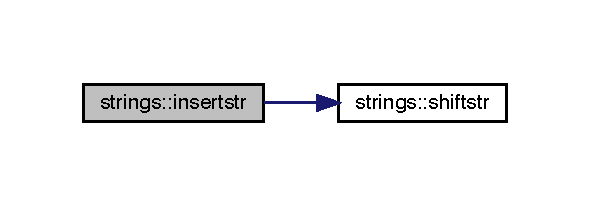
\includegraphics[width=283pt]{namespacestrings_a088c9da339db232b73bcb1f4da4fe5a2_cgraph}
\end{center}
\end{figure}
\mbox{\Hypertarget{namespacestrings_a91d4d50cfe3e624152f5234d89aa6dc5}\label{namespacestrings_a91d4d50cfe3e624152f5234d89aa6dc5}} 
\index{strings@{strings}!is\+\_\+digit@{is\+\_\+digit}}
\index{is\+\_\+digit@{is\+\_\+digit}!strings@{strings}}
\subsubsection{\texorpdfstring{is\+\_\+digit()}{is\_digit()}}
{\footnotesize\ttfamily logical function strings\+::is\+\_\+digit (\begin{DoxyParamCaption}\item[{character}]{ch }\end{DoxyParamCaption})}



Definition at line 662 of file stringmod.\+f95.

\mbox{\Hypertarget{namespacestrings_a3b44a9a233716da3271b645eee79d8f0}\label{namespacestrings_a3b44a9a233716da3271b645eee79d8f0}} 
\index{strings@{strings}!is\+\_\+letter@{is\+\_\+letter}}
\index{is\+\_\+letter@{is\+\_\+letter}!strings@{strings}}
\subsubsection{\texorpdfstring{is\+\_\+letter()}{is\_letter()}}
{\footnotesize\ttfamily logical function strings\+::is\+\_\+letter (\begin{DoxyParamCaption}\item[{character}]{ch }\end{DoxyParamCaption})}



Definition at line 643 of file stringmod.\+f95.

\mbox{\Hypertarget{namespacestrings_ad5a1054d696063fbd4e11ad636796226}\label{namespacestrings_ad5a1054d696063fbd4e11ad636796226}} 
\index{strings@{strings}!lowercase@{lowercase}}
\index{lowercase@{lowercase}!strings@{strings}}
\subsubsection{\texorpdfstring{lowercase()}{lowercase()}}
{\footnotesize\ttfamily character (len=len\+\_\+trim(\hyperlink{_s_o_l_w_e_i_g__misc_8f95_a77a2ca74046c88062aa8333bf1eaca05}{str})) function strings\+::lowercase (\begin{DoxyParamCaption}\item[{character (len=$\ast$)}]{str }\end{DoxyParamCaption})}



Definition at line 363 of file stringmod.\+f95.

\mbox{\Hypertarget{namespacestrings_ad5ead0bc741b619b8e30528ccebbd057}\label{namespacestrings_ad5ead0bc741b619b8e30528ccebbd057}} 
\index{strings@{strings}!match@{match}}
\index{match@{match}!strings@{strings}}
\subsubsection{\texorpdfstring{match()}{match()}}
{\footnotesize\ttfamily subroutine strings\+::match (\begin{DoxyParamCaption}\item[{character(len=$\ast$)}]{str,  }\item[{}]{ipos,  }\item[{}]{imatch }\end{DoxyParamCaption})}



Definition at line 420 of file stringmod.\+f95.

\mbox{\Hypertarget{namespacestrings_a6905131fa6e36e7e719b2f3c5f499d93}\label{namespacestrings_a6905131fa6e36e7e719b2f3c5f499d93}} 
\index{strings@{strings}!parse@{parse}}
\index{parse@{parse}!strings@{strings}}
\subsubsection{\texorpdfstring{parse()}{parse()}}
{\footnotesize\ttfamily subroutine strings\+::parse (\begin{DoxyParamCaption}\item[{character(len=$\ast$)}]{str,  }\item[{character(len=$\ast$)}]{delims,  }\item[{character(len=$\ast$), dimension(\+:)}]{args,  }\item[{}]{nargs }\end{DoxyParamCaption})}



Definition at line 53 of file stringmod.\+f95.

Here is the call graph for this function\+:\nopagebreak
\begin{figure}[H]
\begin{center}
\leavevmode
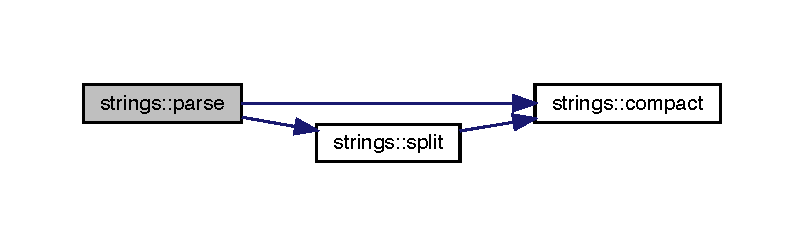
\includegraphics[width=350pt]{namespacestrings_a6905131fa6e36e7e719b2f3c5f499d93_cgraph}
\end{center}
\end{figure}
\mbox{\Hypertarget{namespacestrings_a6c26fe0ca9e11a3ca296f1c350f54f42}\label{namespacestrings_a6c26fe0ca9e11a3ca296f1c350f54f42}} 
\index{strings@{strings}!readline@{readline}}
\index{readline@{readline}!strings@{strings}}
\subsubsection{\texorpdfstring{readline()}{readline()}}
{\footnotesize\ttfamily subroutine strings\+::readline (\begin{DoxyParamCaption}\item[{}]{nunitr,  }\item[{character (len=$\ast$)}]{line,  }\item[{}]{ios }\end{DoxyParamCaption})}



Definition at line 398 of file stringmod.\+f95.

\mbox{\Hypertarget{namespacestrings_a15595b232883855ee75d1044d27694bd}\label{namespacestrings_a15595b232883855ee75d1044d27694bd}} 
\index{strings@{strings}!removesp@{removesp}}
\index{removesp@{removesp}!strings@{strings}}
\subsubsection{\texorpdfstring{removesp()}{removesp()}}
{\footnotesize\ttfamily subroutine strings\+::removesp (\begin{DoxyParamCaption}\item[{character(len=$\ast$)}]{str }\end{DoxyParamCaption})}



Definition at line 130 of file stringmod.\+f95.

\mbox{\Hypertarget{namespacestrings_a351d6a37fa1a55733a40b8c1b0dd686e}\label{namespacestrings_a351d6a37fa1a55733a40b8c1b0dd686e}} 
\index{strings@{strings}!shiftstr@{shiftstr}}
\index{shiftstr@{shiftstr}!strings@{strings}}
\subsubsection{\texorpdfstring{shiftstr()}{shiftstr()}}
{\footnotesize\ttfamily subroutine strings\+::shiftstr (\begin{DoxyParamCaption}\item[{character(len=$\ast$)}]{str,  }\item[{}]{n }\end{DoxyParamCaption})}



Definition at line 239 of file stringmod.\+f95.

\mbox{\Hypertarget{namespacestrings_a12ec697adfa3201deadb7777456db11c}\label{namespacestrings_a12ec697adfa3201deadb7777456db11c}} 
\index{strings@{strings}!split@{split}}
\index{split@{split}!strings@{strings}}
\subsubsection{\texorpdfstring{split()}{split()}}
{\footnotesize\ttfamily subroutine strings\+::split (\begin{DoxyParamCaption}\item[{character(len=$\ast$)}]{str,  }\item[{character(len=$\ast$)}]{delims,  }\item[{character(len=$\ast$)}]{before,  }\item[{character, optional}]{sep }\end{DoxyParamCaption})}



Definition at line 681 of file stringmod.\+f95.

Here is the call graph for this function\+:\nopagebreak
\begin{figure}[H]
\begin{center}
\leavevmode
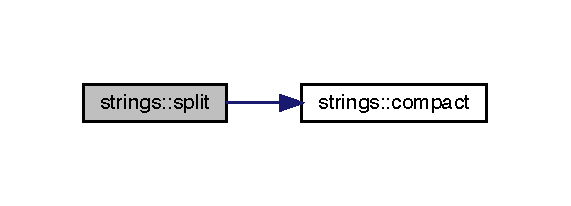
\includegraphics[width=274pt]{namespacestrings_a12ec697adfa3201deadb7777456db11c_cgraph}
\end{center}
\end{figure}
\mbox{\Hypertarget{namespacestrings_a18777b9741e00afdfe3ec5f5fa16ca46}\label{namespacestrings_a18777b9741e00afdfe3ec5f5fa16ca46}} 
\index{strings@{strings}!trimzero@{trimzero}}
\index{trimzero@{trimzero}!strings@{strings}}
\subsubsection{\texorpdfstring{trimzero()}{trimzero()}}
{\footnotesize\ttfamily subroutine strings\+::trimzero (\begin{DoxyParamCaption}\item[{character(len=$\ast$)}]{str }\end{DoxyParamCaption})}



Definition at line 545 of file stringmod.\+f95.

\mbox{\Hypertarget{namespacestrings_a9e805cff1c9339d9c7e7d10808a97e62}\label{namespacestrings_a9e805cff1c9339d9c7e7d10808a97e62}} 
\index{strings@{strings}!uppercase@{uppercase}}
\index{uppercase@{uppercase}!strings@{strings}}
\subsubsection{\texorpdfstring{uppercase()}{uppercase()}}
{\footnotesize\ttfamily character (len=len\+\_\+trim(\hyperlink{_s_o_l_w_e_i_g__misc_8f95_a77a2ca74046c88062aa8333bf1eaca05}{str})) function strings\+::uppercase (\begin{DoxyParamCaption}\item[{character (len=$\ast$)}]{str }\end{DoxyParamCaption})}



Definition at line 328 of file stringmod.\+f95.


\hypertarget{namespacesues__data}{}\section{sues\+\_\+data Module Reference}
\label{namespacesues__data}\index{sues\+\_\+data@{sues\+\_\+data}}
\subsection*{Variables}
\begin{DoxyCompactItemize}
\item 
integer \hyperlink{namespacesues__data_ac6af955be55f5fe026b4ba1ab6ec480e}{tstep}
\item 
integer \hyperlink{namespacesues__data_ab28124e60c813d253c9b095050fe3ebe}{nsh}
\item 
integer \hyperlink{namespacesues__data_a1fd9bd64afb3354e7e90260d0f0c6e94}{nsd}
\item 
integer \hyperlink{namespacesues__data_aa6fc5b2432c730d5b950fa2b37ac4630}{nsdorig}
\item 
integer \hyperlink{namespacesues__data_a91f69564eaa9aa824c0043d532502229}{t\+\_\+interval}
\item 
integer \hyperlink{namespacesues__data_aee4c8e6d4c94a2af0599fb1cd40f51ed}{nper}
\item 
integer \hyperlink{namespacesues__data_a699b9583b9326461b9220d76056b85b5}{nperestm}
\item 
real(kind(1d0)) \hyperlink{namespacesues__data_ab2070158f8b88b8f7835232841061718}{nsh\+\_\+real}
\item 
real(kind(1d0)) \hyperlink{namespacesues__data_a81a241a978fdd040dee716c4e68dc786}{tstep\+\_\+real}
\item 
real(kind(1d0)) \hyperlink{namespacesues__data_a130a64aeadd8ca145f5ec2d1416174f5}{nper\+\_\+real}
\item 
real(kind(1d0)) \hyperlink{namespacesues__data_aad88365e0d1f6430e9ac39dd331048c1}{nperestm\+\_\+real}
\item 
real(kind(1d0)) \hyperlink{namespacesues__data_a6e2f669999914372fd2de922c917e6dc}{halftimestep}
\item 
integer \hyperlink{namespacesues__data_a1005846b0d388b51d731e6d5e404e2d6}{stabilitymethod}
\item 
integer \hyperlink{namespacesues__data_a9dff10e1f001cc8241e5d1d72a4beeb2}{roughlenheatmethod}
\item 
integer \hyperlink{namespacesues__data_ae5a31f2a4addf36e077f1e18eabf6052}{in}
\item 
integer \hyperlink{namespacesues__data_a38a6478771abe06a6cf4334fe858c0ef}{is}
\item 
integer \hyperlink{namespacesues__data_a1780a57f30571faa7263e9cd248a8dd0}{aerodynamicresistancemethod} =2
\item 
integer \hyperlink{namespacesues__data_a64de572d5505a9ff4174a4703db24a9e}{ie\+\_\+start}
\item 
integer \hyperlink{namespacesues__data_a7f97cb4ce39cccee777bae8977654da7}{ie\+\_\+end}
\item 
real(kind(1d0)), dimension(2) \hyperlink{namespacesues__data_a08d117cca68ee0e84a8b286a038434c6}{surplusevap}
\item 
real(kind(1d0)) \hyperlink{namespacesues__data_aafb79a529ff89254c1399e96d77a5fe0}{flowchange}
\item 
real(kind(1d0)) \hyperlink{namespacesues__data_ab2dc1363710dd5d250384fe643279fd7}{pipecapacity}
\item 
real(kind(1d0)) \hyperlink{namespacesues__data_a92f648948ca3627c9bc8442568c4bba1}{runofftowater}
\item 
real(kind(1d0)) \hyperlink{namespacesues__data_a08339a22d19b4766db4ad302512459ba}{smcap}
\item 
real(kind(1d0)) \hyperlink{namespacesues__data_ac26ae7a72cca3b9be662578e90231c4a}{soildensity}
\item 
real(kind(1d0)) \hyperlink{namespacesues__data_ac09e3f2b843f21d26f4f106cb450df06}{soildepthmeas}
\item 
real(kind(1d0)) \hyperlink{namespacesues__data_a5eb41bdf4cc30812b303de4d2acceb67}{soilrocks}
\item 
real(kind(1d0)) \hyperlink{namespacesues__data_a9d6a1e2ae7fe7c36fb4aaa9e2e3c2137}{surfacearea}
\item 
real(kind(1d0)) \hyperlink{namespacesues__data_a77ef6a343e9a419577fa473535ab3c16}{surfacearea\+\_\+ha}
\item 
real(kind(1d0)) \hyperlink{namespacesues__data_a6433e676b899356c4023713d7a5ab589}{waterbodytype}
\item 
real(kind(1d0)) \hyperlink{namespacesues__data_adf49f9058cfb8894abba11870ace90bf}{waterstorcap}
\item 
real(kind(1d0)) \hyperlink{namespacesues__data_a167fa54ed7df9e23b3dac81232961fa3}{wuareaevetr\+\_\+m2}
\item 
real(kind(1d0)) \hyperlink{namespacesues__data_a3dd16ee1aeeae265f322b0982f33a321}{wuareadectr\+\_\+m2}
\item 
real(kind(1d0)) \hyperlink{namespacesues__data_a9d58cea1a78af7ae81ee097bde9e0ef4}{wuareagrass\+\_\+m2}
\item 
real(kind(1d0)) \hyperlink{namespacesues__data_a4145456981d7aaa8f5b19ab3ea5f1781}{wuareatotal\+\_\+m2}
\item 
real(kind(1d0)) \hyperlink{namespacesues__data_a6aa0ce59c7eee4b94b9ee86ac5b555d0}{wu\+\_\+evetr}
\item 
real(kind(1d0)) \hyperlink{namespacesues__data_a087f298012279c621f24a283b360d592}{wu\+\_\+dectr}
\item 
real(kind(1d0)) \hyperlink{namespacesues__data_a56315a7303bf70155e92ead9b64493c2}{wu\+\_\+grass}
\item 
real(kind(1d0)) \hyperlink{namespacesues__data_a2c84a8e635e90b198dc0fd4c93c51ba4}{additionalwater}
\item 
real(kind(1d0)) \hyperlink{namespacesues__data_a79ed0c9098d69fcbc6ad9a95fddaf013}{ch\+\_\+per\+\_\+interval}
\item 
real(kind(1d0)) \hyperlink{namespacesues__data_af62ec721dfd084ec5bce9224750e1330}{chsnow\+\_\+per\+\_\+interval}
\item 
real(kind(1d0)) \hyperlink{namespacesues__data_a6f3357b61d4b1a639e99356c6a49ea6e}{di\+\_\+dt}
\item 
real(kind(1d0)) \hyperlink{namespacesues__data_aad693b9bca68a54522874f01bd0f2a18}{dr\+\_\+per\+\_\+interval}
\item 
real(kind(1d0)) \hyperlink{namespacesues__data_ac9d7bd8852ff457c5d8dd2588910ebf3}{ev\+\_\+per\+\_\+interval}
\item 
real(kind(1d0)) \hyperlink{namespacesues__data_a1848f093a3dd5ebdc1da775e9cda8509}{surf\+\_\+chang\+\_\+per\+\_\+tstep}
\item 
real(kind(1d0)) \hyperlink{namespacesues__data_a82ac11b95b008fb43921aac3b503efad}{tot\+\_\+chang\+\_\+per\+\_\+tstep}
\item 
real(kind(1d0)) \hyperlink{namespacesues__data_a9a093b62067234bd553e776c06ac4df9}{nwstate\+\_\+per\+\_\+tstep}
\item 
real(kind(1d0)) \hyperlink{namespacesues__data_abdb761c4b6b03cace33c5c54eb3607b2}{state\+\_\+per\+\_\+tstep}
\item 
real(kind(1d0)) \hyperlink{namespacesues__data_a96e76d9edd6c97fcdbc8f73047e189f3}{drain\+\_\+per\+\_\+tstep}
\item 
real(kind(1d0)) \hyperlink{namespacesues__data_a15eb03975ee429099b923fc02a2577ca}{runoff\+\_\+per\+\_\+tstep}
\item 
real(kind(1d0)) \hyperlink{namespacesues__data_a3b42551207483efdea0f50bba253afe4}{runoffsoil\+\_\+per\+\_\+tstep}
\item 
real(kind(1d0)) \hyperlink{namespacesues__data_a11bc80be13a121686d39d355d6c98aa9}{ev\+\_\+per\+\_\+tstep}
\item 
real(kind(1d0)) \hyperlink{namespacesues__data_a8506404b27e8b0ded77802f2ab475928}{qe\+\_\+per\+\_\+tstep}
\item 
real(kind(1d0)) \hyperlink{namespacesues__data_a9ddcc1842e650815dfc06fa4a3bf6a78}{p\+\_\+mm}
\item 
real(kind(1d0)) \hyperlink{namespacesues__data_aa2d35158f50e5437170a36712c99a891}{pin}
\item 
real(kind(1d0)) \hyperlink{namespacesues__data_a0489c46c970c2dd6ecdf0af0e11dee21}{planf}
\item 
real(kind(1d0)) \hyperlink{namespacesues__data_a90293da57db1b1a3a4bc0979d2005640}{rb}
\item 
real(kind(1d0)) \hyperlink{namespacesues__data_ac376fe6389c7367c307fce12d816009c}{runoffagimpervious}
\item 
real(kind(1d0)) \hyperlink{namespacesues__data_ac2654954c97c2cbba667e51f44850250}{runoffagveg}
\item 
real(kind(1d0)) \hyperlink{namespacesues__data_a0fce415bc7210db0cfe37ded2d8c1ef5}{runoffwaterbody}
\item 
real(kind(1d0)) \hyperlink{namespacesues__data_a20b9d66de8207bb6709f620aebc98b17}{runoffpipes}
\item 
real(kind(1d0)) \hyperlink{namespacesues__data_a56bf7a98188b09dfcd2c9daed991f1b0}{runoffagimpervious\+\_\+m3}
\item 
real(kind(1d0)) \hyperlink{namespacesues__data_a030c38cf6a2cc1b2121491399a0353a5}{runoffagveg\+\_\+m3}
\item 
real(kind(1d0)) \hyperlink{namespacesues__data_abc5b5ae18f30abb3a858e2e24e1e99d7}{runoffwaterbody\+\_\+m3}
\item 
real(kind(1d0)) \hyperlink{namespacesues__data_ac5a856a3cdf4ba0b3a9150f2a08bb13d}{runoffpipes\+\_\+m3}
\item 
real(kind(1d0)) \hyperlink{namespacesues__data_a3e74512061da577d1697d50324b5ea28}{runoff\+\_\+per\+\_\+interval}
\item 
real(kind(1d0)) \hyperlink{namespacesues__data_af0fed458b1eefc0164c4ffb6d6e2d1a2}{addimpervious}
\item 
real(kind(1d0)) \hyperlink{namespacesues__data_a2553d0e5b7218422246f2078b379fed5}{addveg}
\item 
real(kind(1d0)) \hyperlink{namespacesues__data_aa314ccdf6d41a3901fa922504f030203}{addwaterbody}
\item 
real(kind(1d0)) \hyperlink{namespacesues__data_a58a8108dff93f602ad2ef840fef9395f}{addpipes}
\item 
real(kind(1d0)) \hyperlink{namespacesues__data_ae3658e6cd4c5115a1a9f8ea57cf6f6b1}{runoffsoil\+\_\+per\+\_\+interval}
\item 
real(kind(1d0)) \hyperlink{namespacesues__data_a63a7c6317d6086404efee7da0d9be4da}{qe\+\_\+per\+\_\+interval}
\item 
real(kind(1d0)) \hyperlink{namespacesues__data_ada5a214d0c4d5da587baa5f8de1da6d9}{soilmoistcap}
\item 
real(kind(1d0)) \hyperlink{namespacesues__data_afa546047f4e8bd032736a6915fe1cffd}{soilstate}
\item 
real(kind(1d0)) \hyperlink{namespacesues__data_a2de83c53a6d33bd6f917cf0418fe3d50}{st\+\_\+per\+\_\+interval}
\item 
real(kind(1d0)) \hyperlink{namespacesues__data_ac93567a8ca56d05105523626613f5cc4}{surpluswaterbody}
\item 
real(kind(1d0)) \hyperlink{namespacesues__data_a45028b146a251db48e2682b486211654}{tlv\+\_\+sub}
\item 
real(kind(1d0)) \hyperlink{namespacesues__data_aa663cd30d361709a541de0a9d406557e}{overuse} =0
\item 
real(kind(1d0)) \hyperlink{namespacesues__data_a738f60744a0e91f90a050542ad946898}{zh}
\item 
real(kind(1d0)) \hyperlink{namespacesues__data_ae76235b1ac6a388886f63eb27a0905dd}{h}
\item 
real(kind(1d0)) \hyperlink{namespacesues__data_a7623dce80601c63b78d744b4a5036ad2}{l\+\_\+mod}
\item 
real(kind(1d0)) \hyperlink{namespacesues__data_ab35a12f588d9dfb72d0ec039e806d3bb}{psim}
\item 
real(kind(1d0)) \hyperlink{namespacesues__data_a6d5d62e6767411fff0b1641fe6cbf1f9}{psyh}
\item 
real(kind(1d0)) \hyperlink{namespacesues__data_aafce3a183c34dd4df5268cdbfc8aea24}{ra}
\item 
real(kind(1d0)) \hyperlink{namespacesues__data_a2a84935439f246e72f5de7bd752888f1}{rasnow}
\item 
real(kind(1d0)) \hyperlink{namespacesues__data_a6d0dd8d535aa36ca406b9c4ba99caef6}{tstar}
\item 
real(kind(1d0)) \hyperlink{namespacesues__data_a3422c30d52ea500ca138d13670403a50}{ustar}
\item 
real(kind(1d0)) \hyperlink{namespacesues__data_a7c7f724d95b99e3b5ff7e350e70f1fb1}{z0\+\_\+gis}
\item 
real(kind(1d0)) \hyperlink{namespacesues__data_a678cac1e19ddb70f811693772c031f0c}{resistsurf}
\item 
real(kind(1d0)) \hyperlink{namespacesues__data_a7ef0beda82e8b6758f37961b50f91b8a}{gdq}
\item 
real(kind(1d0)) \hyperlink{namespacesues__data_aa14586435e8c54f775a51aa1dd21ef28}{qnm}
\item 
real(kind(1d0)) \hyperlink{namespacesues__data_a3ad79feef0770aefcae45775fa0c22c8}{gq}
\item 
real(kind(1d0)) \hyperlink{namespacesues__data_afdcda32590540b1055ac240cd92e9325}{gtemp}
\item 
real(kind(1d0)) \hyperlink{namespacesues__data_a4206a1be622f71796ce77db00ec3d459}{gl}
\item 
real(kind(1d0)) \hyperlink{namespacesues__data_a435acd94af1e3a271f4ee348ac811ad4}{sdp}
\item 
real(kind(1d0)) \hyperlink{namespacesues__data_ac73de7c829233718bfd143f4346adf70}{smd}
\item 
real(kind(1d0)) \hyperlink{namespacesues__data_adfce8b9e1538d8a1629df9963a7a6df0}{vsmd}
\item 
real(kind(1d0)) \hyperlink{namespacesues__data_a5eb7587d26ec3542141102660d22dd33}{gs}
\item 
real(kind(1d0)) \hyperlink{namespacesues__data_a0aca98063df71052382d5ab58c2f0d19}{gsc}
\item 
real(kind(1d0)) \hyperlink{namespacesues__data_ae3375f2161517eabda778cd0642076c5}{rss}
\item 
real(kind(1d0)) \hyperlink{namespacesues__data_a79ee74466d17ed05bb20f195934f383b}{vdrc}
\item 
real(kind(1d0)) \hyperlink{namespacesues__data_a06a4500745768a4bcf4886312a028e0c}{numpm}
\item 
real(kind(1d0)) \hyperlink{namespacesues__data_a77243f6b1c7d2baecb0d13f5d98b4318}{sp}
\item 
real(kind(1d0)) \hyperlink{namespacesues__data_ade8fa0a70d4bdc01712ae9438602f21e}{sae}
\item 
real(kind(1d0)) \hyperlink{namespacesues__data_a879c9f9f7cf8597fe30edea62a95bcdd}{ev}
\item 
real(kind(1d0)) \hyperlink{namespacesues__data_a590af4833961785e70adbad8cec1aa66}{rst}
\item 
real(kind(1d0)) \hyperlink{namespacesues__data_a9dfa646ad79f2eadc90c544d5ad4462c}{qeph}
\item 
real(kind(1d0)) \hyperlink{namespacesues__data_ae467db694bf0c56a1afbee403a0d8907}{qeout}
\item 
real(kind(1d0)), dimension(\+:), allocatable \hyperlink{namespacesues__data_a891cda3d0ef1f628e7dd9a185f00fc6c}{qhforcbl}
\item 
real(kind(1d0)), dimension(\+:), allocatable \hyperlink{namespacesues__data_a08451f44609cb386788368a9136432c7}{qeforcbl}
\item 
integer \hyperlink{namespacesues__data_a2333d97226ad99ef4b17125ad7c3b205}{qh\+\_\+choice}
\item 
real(kind(1d0)) \hyperlink{namespacesues__data_ad2e4c4ffe627921b28183c9f4d8789fd}{ext\+\_\+wu}
\item 
real(kind(1d0)) \hyperlink{namespacesues__data_abc299ffec1296474197ca5a9afb4b254}{faut}
\item 
real(kind(1d0)) \hyperlink{namespacesues__data_affbedb6f34d747605bf529fd2d80d4c7}{int\+\_\+wu}
\item 
real(kind(1d0)) \hyperlink{namespacesues__data_aec92653b01eece5fbbb4f1cdfa3575cf}{irrfracconif}
\item 
real(kind(1d0)) \hyperlink{namespacesues__data_aa6d49b1ef69f02f3bd0334c0d50d9a30}{irrfracdecid}
\item 
real(kind(1d0)) \hyperlink{namespacesues__data_ac09560182eb4e8e83479a33c9ea2f52b}{irrfracgrass}
\item 
real(kind(1d0)) \hyperlink{namespacesues__data_aaec40541d3458d50a5e554aa1ca0848b}{internalwateruse\+\_\+h}
\item 
real(kind(1d0)), dimension(7) \hyperlink{namespacesues__data_aaf929b9a25878b781ca0c2069b3e9468}{daywatper}
\item 
real(kind(1d0)), dimension(7) \hyperlink{namespacesues__data_a55dbeb9abd22aa41d295c4348a2fb6de}{daywat}
\item 
real(kind(1d0)), dimension(0\+:23, 2) \hyperlink{namespacesues__data_a5926d0d936d383d4f839d9e7bcc65f48}{wuprofm}
\item 
real(kind(1d0)), dimension(0\+:23, 2) \hyperlink{namespacesues__data_a8b58e7f44021d419ca3e9da1c2a8db49}{wuprofa}
\item 
real(kind(1d0)), dimension(3) \hyperlink{namespacesues__data_a1ddda58bf0af48716e6e89efefa42b47}{ie\+\_\+a}
\item 
real(kind(1d0)), dimension(3) \hyperlink{namespacesues__data_acc07bf45b728dde4f2c1e0063f79808e}{ie\+\_\+m}
\end{DoxyCompactItemize}


\subsection{Variable Documentation}
\mbox{\Hypertarget{namespacesues__data_af0fed458b1eefc0164c4ffb6d6e2d1a2}\label{namespacesues__data_af0fed458b1eefc0164c4ffb6d6e2d1a2}} 
\index{sues\+\_\+data@{sues\+\_\+data}!addimpervious@{addimpervious}}
\index{addimpervious@{addimpervious}!sues\+\_\+data@{sues\+\_\+data}}
\subsubsection{\texorpdfstring{addimpervious}{addimpervious}}
{\footnotesize\ttfamily real (kind(1d0)) sues\+\_\+data\+::addimpervious}



Definition at line 1327 of file L\+U\+M\+P\+S\+\_\+\+Module\+\_\+constants.\+f95.

\mbox{\Hypertarget{namespacesues__data_a2c84a8e635e90b198dc0fd4c93c51ba4}\label{namespacesues__data_a2c84a8e635e90b198dc0fd4c93c51ba4}} 
\index{sues\+\_\+data@{sues\+\_\+data}!additionalwater@{additionalwater}}
\index{additionalwater@{additionalwater}!sues\+\_\+data@{sues\+\_\+data}}
\subsubsection{\texorpdfstring{additionalwater}{additionalwater}}
{\footnotesize\ttfamily real (kind(1d0)) sues\+\_\+data\+::additionalwater}



Definition at line 1327 of file L\+U\+M\+P\+S\+\_\+\+Module\+\_\+constants.\+f95.

\mbox{\Hypertarget{namespacesues__data_a58a8108dff93f602ad2ef840fef9395f}\label{namespacesues__data_a58a8108dff93f602ad2ef840fef9395f}} 
\index{sues\+\_\+data@{sues\+\_\+data}!addpipes@{addpipes}}
\index{addpipes@{addpipes}!sues\+\_\+data@{sues\+\_\+data}}
\subsubsection{\texorpdfstring{addpipes}{addpipes}}
{\footnotesize\ttfamily real (kind(1d0)) sues\+\_\+data\+::addpipes}



Definition at line 1327 of file L\+U\+M\+P\+S\+\_\+\+Module\+\_\+constants.\+f95.

\mbox{\Hypertarget{namespacesues__data_a2553d0e5b7218422246f2078b379fed5}\label{namespacesues__data_a2553d0e5b7218422246f2078b379fed5}} 
\index{sues\+\_\+data@{sues\+\_\+data}!addveg@{addveg}}
\index{addveg@{addveg}!sues\+\_\+data@{sues\+\_\+data}}
\subsubsection{\texorpdfstring{addveg}{addveg}}
{\footnotesize\ttfamily real (kind(1d0)) sues\+\_\+data\+::addveg}



Definition at line 1327 of file L\+U\+M\+P\+S\+\_\+\+Module\+\_\+constants.\+f95.

\mbox{\Hypertarget{namespacesues__data_aa314ccdf6d41a3901fa922504f030203}\label{namespacesues__data_aa314ccdf6d41a3901fa922504f030203}} 
\index{sues\+\_\+data@{sues\+\_\+data}!addwaterbody@{addwaterbody}}
\index{addwaterbody@{addwaterbody}!sues\+\_\+data@{sues\+\_\+data}}
\subsubsection{\texorpdfstring{addwaterbody}{addwaterbody}}
{\footnotesize\ttfamily real (kind(1d0)) sues\+\_\+data\+::addwaterbody}



Definition at line 1327 of file L\+U\+M\+P\+S\+\_\+\+Module\+\_\+constants.\+f95.

\mbox{\Hypertarget{namespacesues__data_a1780a57f30571faa7263e9cd248a8dd0}\label{namespacesues__data_a1780a57f30571faa7263e9cd248a8dd0}} 
\index{sues\+\_\+data@{sues\+\_\+data}!aerodynamicresistancemethod@{aerodynamicresistancemethod}}
\index{aerodynamicresistancemethod@{aerodynamicresistancemethod}!sues\+\_\+data@{sues\+\_\+data}}
\subsubsection{\texorpdfstring{aerodynamicresistancemethod}{aerodynamicresistancemethod}}
{\footnotesize\ttfamily integer sues\+\_\+data\+::aerodynamicresistancemethod =2}



Definition at line 1298 of file L\+U\+M\+P\+S\+\_\+\+Module\+\_\+constants.\+f95.

\mbox{\Hypertarget{namespacesues__data_a79ed0c9098d69fcbc6ad9a95fddaf013}\label{namespacesues__data_a79ed0c9098d69fcbc6ad9a95fddaf013}} 
\index{sues\+\_\+data@{sues\+\_\+data}!ch\+\_\+per\+\_\+interval@{ch\+\_\+per\+\_\+interval}}
\index{ch\+\_\+per\+\_\+interval@{ch\+\_\+per\+\_\+interval}!sues\+\_\+data@{sues\+\_\+data}}
\subsubsection{\texorpdfstring{ch\+\_\+per\+\_\+interval}{ch\_per\_interval}}
{\footnotesize\ttfamily real (kind(1d0)) sues\+\_\+data\+::ch\+\_\+per\+\_\+interval}



Definition at line 1327 of file L\+U\+M\+P\+S\+\_\+\+Module\+\_\+constants.\+f95.

\mbox{\Hypertarget{namespacesues__data_af62ec721dfd084ec5bce9224750e1330}\label{namespacesues__data_af62ec721dfd084ec5bce9224750e1330}} 
\index{sues\+\_\+data@{sues\+\_\+data}!chsnow\+\_\+per\+\_\+interval@{chsnow\+\_\+per\+\_\+interval}}
\index{chsnow\+\_\+per\+\_\+interval@{chsnow\+\_\+per\+\_\+interval}!sues\+\_\+data@{sues\+\_\+data}}
\subsubsection{\texorpdfstring{chsnow\+\_\+per\+\_\+interval}{chsnow\_per\_interval}}
{\footnotesize\ttfamily real (kind(1d0)) sues\+\_\+data\+::chsnow\+\_\+per\+\_\+interval}



Definition at line 1327 of file L\+U\+M\+P\+S\+\_\+\+Module\+\_\+constants.\+f95.

\mbox{\Hypertarget{namespacesues__data_a55dbeb9abd22aa41d295c4348a2fb6de}\label{namespacesues__data_a55dbeb9abd22aa41d295c4348a2fb6de}} 
\index{sues\+\_\+data@{sues\+\_\+data}!daywat@{daywat}}
\index{daywat@{daywat}!sues\+\_\+data@{sues\+\_\+data}}
\subsubsection{\texorpdfstring{daywat}{daywat}}
{\footnotesize\ttfamily real(kind(1d0)), dimension(7) sues\+\_\+data\+::daywat}



Definition at line 1420 of file L\+U\+M\+P\+S\+\_\+\+Module\+\_\+constants.\+f95.

\mbox{\Hypertarget{namespacesues__data_aaf929b9a25878b781ca0c2069b3e9468}\label{namespacesues__data_aaf929b9a25878b781ca0c2069b3e9468}} 
\index{sues\+\_\+data@{sues\+\_\+data}!daywatper@{daywatper}}
\index{daywatper@{daywatper}!sues\+\_\+data@{sues\+\_\+data}}
\subsubsection{\texorpdfstring{daywatper}{daywatper}}
{\footnotesize\ttfamily real(kind(1d0)), dimension(7) sues\+\_\+data\+::daywatper}



Definition at line 1420 of file L\+U\+M\+P\+S\+\_\+\+Module\+\_\+constants.\+f95.

\mbox{\Hypertarget{namespacesues__data_a6f3357b61d4b1a639e99356c6a49ea6e}\label{namespacesues__data_a6f3357b61d4b1a639e99356c6a49ea6e}} 
\index{sues\+\_\+data@{sues\+\_\+data}!di\+\_\+dt@{di\+\_\+dt}}
\index{di\+\_\+dt@{di\+\_\+dt}!sues\+\_\+data@{sues\+\_\+data}}
\subsubsection{\texorpdfstring{di\+\_\+dt}{di\_dt}}
{\footnotesize\ttfamily real (kind(1d0)) sues\+\_\+data\+::di\+\_\+dt}



Definition at line 1327 of file L\+U\+M\+P\+S\+\_\+\+Module\+\_\+constants.\+f95.

\mbox{\Hypertarget{namespacesues__data_aad693b9bca68a54522874f01bd0f2a18}\label{namespacesues__data_aad693b9bca68a54522874f01bd0f2a18}} 
\index{sues\+\_\+data@{sues\+\_\+data}!dr\+\_\+per\+\_\+interval@{dr\+\_\+per\+\_\+interval}}
\index{dr\+\_\+per\+\_\+interval@{dr\+\_\+per\+\_\+interval}!sues\+\_\+data@{sues\+\_\+data}}
\subsubsection{\texorpdfstring{dr\+\_\+per\+\_\+interval}{dr\_per\_interval}}
{\footnotesize\ttfamily real (kind(1d0)) sues\+\_\+data\+::dr\+\_\+per\+\_\+interval}



Definition at line 1327 of file L\+U\+M\+P\+S\+\_\+\+Module\+\_\+constants.\+f95.

\mbox{\Hypertarget{namespacesues__data_a96e76d9edd6c97fcdbc8f73047e189f3}\label{namespacesues__data_a96e76d9edd6c97fcdbc8f73047e189f3}} 
\index{sues\+\_\+data@{sues\+\_\+data}!drain\+\_\+per\+\_\+tstep@{drain\+\_\+per\+\_\+tstep}}
\index{drain\+\_\+per\+\_\+tstep@{drain\+\_\+per\+\_\+tstep}!sues\+\_\+data@{sues\+\_\+data}}
\subsubsection{\texorpdfstring{drain\+\_\+per\+\_\+tstep}{drain\_per\_tstep}}
{\footnotesize\ttfamily real (kind(1d0)) sues\+\_\+data\+::drain\+\_\+per\+\_\+tstep}



Definition at line 1327 of file L\+U\+M\+P\+S\+\_\+\+Module\+\_\+constants.\+f95.

\mbox{\Hypertarget{namespacesues__data_a879c9f9f7cf8597fe30edea62a95bcdd}\label{namespacesues__data_a879c9f9f7cf8597fe30edea62a95bcdd}} 
\index{sues\+\_\+data@{sues\+\_\+data}!ev@{ev}}
\index{ev@{ev}!sues\+\_\+data@{sues\+\_\+data}}
\subsubsection{\texorpdfstring{ev}{ev}}
{\footnotesize\ttfamily real (kind(1d0)) sues\+\_\+data\+::ev}



Definition at line 1398 of file L\+U\+M\+P\+S\+\_\+\+Module\+\_\+constants.\+f95.

\mbox{\Hypertarget{namespacesues__data_ac9d7bd8852ff457c5d8dd2588910ebf3}\label{namespacesues__data_ac9d7bd8852ff457c5d8dd2588910ebf3}} 
\index{sues\+\_\+data@{sues\+\_\+data}!ev\+\_\+per\+\_\+interval@{ev\+\_\+per\+\_\+interval}}
\index{ev\+\_\+per\+\_\+interval@{ev\+\_\+per\+\_\+interval}!sues\+\_\+data@{sues\+\_\+data}}
\subsubsection{\texorpdfstring{ev\+\_\+per\+\_\+interval}{ev\_per\_interval}}
{\footnotesize\ttfamily real (kind(1d0)) sues\+\_\+data\+::ev\+\_\+per\+\_\+interval}



Definition at line 1327 of file L\+U\+M\+P\+S\+\_\+\+Module\+\_\+constants.\+f95.

\mbox{\Hypertarget{namespacesues__data_a11bc80be13a121686d39d355d6c98aa9}\label{namespacesues__data_a11bc80be13a121686d39d355d6c98aa9}} 
\index{sues\+\_\+data@{sues\+\_\+data}!ev\+\_\+per\+\_\+tstep@{ev\+\_\+per\+\_\+tstep}}
\index{ev\+\_\+per\+\_\+tstep@{ev\+\_\+per\+\_\+tstep}!sues\+\_\+data@{sues\+\_\+data}}
\subsubsection{\texorpdfstring{ev\+\_\+per\+\_\+tstep}{ev\_per\_tstep}}
{\footnotesize\ttfamily real (kind(1d0)) sues\+\_\+data\+::ev\+\_\+per\+\_\+tstep}



Definition at line 1327 of file L\+U\+M\+P\+S\+\_\+\+Module\+\_\+constants.\+f95.

\mbox{\Hypertarget{namespacesues__data_ad2e4c4ffe627921b28183c9f4d8789fd}\label{namespacesues__data_ad2e4c4ffe627921b28183c9f4d8789fd}} 
\index{sues\+\_\+data@{sues\+\_\+data}!ext\+\_\+wu@{ext\+\_\+wu}}
\index{ext\+\_\+wu@{ext\+\_\+wu}!sues\+\_\+data@{sues\+\_\+data}}
\subsubsection{\texorpdfstring{ext\+\_\+wu}{ext\_wu}}
{\footnotesize\ttfamily real (kind(1d0)) sues\+\_\+data\+::ext\+\_\+wu}



Definition at line 1411 of file L\+U\+M\+P\+S\+\_\+\+Module\+\_\+constants.\+f95.

\mbox{\Hypertarget{namespacesues__data_abc299ffec1296474197ca5a9afb4b254}\label{namespacesues__data_abc299ffec1296474197ca5a9afb4b254}} 
\index{sues\+\_\+data@{sues\+\_\+data}!faut@{faut}}
\index{faut@{faut}!sues\+\_\+data@{sues\+\_\+data}}
\subsubsection{\texorpdfstring{faut}{faut}}
{\footnotesize\ttfamily real (kind(1d0)) sues\+\_\+data\+::faut}



Definition at line 1411 of file L\+U\+M\+P\+S\+\_\+\+Module\+\_\+constants.\+f95.

\mbox{\Hypertarget{namespacesues__data_aafb79a529ff89254c1399e96d77a5fe0}\label{namespacesues__data_aafb79a529ff89254c1399e96d77a5fe0}} 
\index{sues\+\_\+data@{sues\+\_\+data}!flowchange@{flowchange}}
\index{flowchange@{flowchange}!sues\+\_\+data@{sues\+\_\+data}}
\subsubsection{\texorpdfstring{flowchange}{flowchange}}
{\footnotesize\ttfamily real (kind(1d0)) sues\+\_\+data\+::flowchange}



Definition at line 1307 of file L\+U\+M\+P\+S\+\_\+\+Module\+\_\+constants.\+f95.

\mbox{\Hypertarget{namespacesues__data_a7ef0beda82e8b6758f37961b50f91b8a}\label{namespacesues__data_a7ef0beda82e8b6758f37961b50f91b8a}} 
\index{sues\+\_\+data@{sues\+\_\+data}!gdq@{gdq}}
\index{gdq@{gdq}!sues\+\_\+data@{sues\+\_\+data}}
\subsubsection{\texorpdfstring{gdq}{gdq}}
{\footnotesize\ttfamily real (kind(1d0)) sues\+\_\+data\+::gdq}



Definition at line 1384 of file L\+U\+M\+P\+S\+\_\+\+Module\+\_\+constants.\+f95.

\mbox{\Hypertarget{namespacesues__data_a4206a1be622f71796ce77db00ec3d459}\label{namespacesues__data_a4206a1be622f71796ce77db00ec3d459}} 
\index{sues\+\_\+data@{sues\+\_\+data}!gl@{gl}}
\index{gl@{gl}!sues\+\_\+data@{sues\+\_\+data}}
\subsubsection{\texorpdfstring{gl}{gl}}
{\footnotesize\ttfamily real (kind(1d0)) sues\+\_\+data\+::gl}



Definition at line 1384 of file L\+U\+M\+P\+S\+\_\+\+Module\+\_\+constants.\+f95.

\mbox{\Hypertarget{namespacesues__data_a3ad79feef0770aefcae45775fa0c22c8}\label{namespacesues__data_a3ad79feef0770aefcae45775fa0c22c8}} 
\index{sues\+\_\+data@{sues\+\_\+data}!gq@{gq}}
\index{gq@{gq}!sues\+\_\+data@{sues\+\_\+data}}
\subsubsection{\texorpdfstring{gq}{gq}}
{\footnotesize\ttfamily real (kind(1d0)) sues\+\_\+data\+::gq}



Definition at line 1384 of file L\+U\+M\+P\+S\+\_\+\+Module\+\_\+constants.\+f95.

\mbox{\Hypertarget{namespacesues__data_a5eb7587d26ec3542141102660d22dd33}\label{namespacesues__data_a5eb7587d26ec3542141102660d22dd33}} 
\index{sues\+\_\+data@{sues\+\_\+data}!gs@{gs}}
\index{gs@{gs}!sues\+\_\+data@{sues\+\_\+data}}
\subsubsection{\texorpdfstring{gs}{gs}}
{\footnotesize\ttfamily real (kind(1d0)) sues\+\_\+data\+::gs}



Definition at line 1384 of file L\+U\+M\+P\+S\+\_\+\+Module\+\_\+constants.\+f95.

\mbox{\Hypertarget{namespacesues__data_a0aca98063df71052382d5ab58c2f0d19}\label{namespacesues__data_a0aca98063df71052382d5ab58c2f0d19}} 
\index{sues\+\_\+data@{sues\+\_\+data}!gsc@{gsc}}
\index{gsc@{gsc}!sues\+\_\+data@{sues\+\_\+data}}
\subsubsection{\texorpdfstring{gsc}{gsc}}
{\footnotesize\ttfamily real (kind(1d0)) sues\+\_\+data\+::gsc}



Definition at line 1384 of file L\+U\+M\+P\+S\+\_\+\+Module\+\_\+constants.\+f95.

\mbox{\Hypertarget{namespacesues__data_afdcda32590540b1055ac240cd92e9325}\label{namespacesues__data_afdcda32590540b1055ac240cd92e9325}} 
\index{sues\+\_\+data@{sues\+\_\+data}!gtemp@{gtemp}}
\index{gtemp@{gtemp}!sues\+\_\+data@{sues\+\_\+data}}
\subsubsection{\texorpdfstring{gtemp}{gtemp}}
{\footnotesize\ttfamily real (kind(1d0)) sues\+\_\+data\+::gtemp}



Definition at line 1384 of file L\+U\+M\+P\+S\+\_\+\+Module\+\_\+constants.\+f95.

\mbox{\Hypertarget{namespacesues__data_ae76235b1ac6a388886f63eb27a0905dd}\label{namespacesues__data_ae76235b1ac6a388886f63eb27a0905dd}} 
\index{sues\+\_\+data@{sues\+\_\+data}!h@{h}}
\index{h@{h}!sues\+\_\+data@{sues\+\_\+data}}
\subsubsection{\texorpdfstring{h}{h}}
{\footnotesize\ttfamily real (kind(1d0)) sues\+\_\+data\+::h}



Definition at line 1373 of file L\+U\+M\+P\+S\+\_\+\+Module\+\_\+constants.\+f95.

\mbox{\Hypertarget{namespacesues__data_a6e2f669999914372fd2de922c917e6dc}\label{namespacesues__data_a6e2f669999914372fd2de922c917e6dc}} 
\index{sues\+\_\+data@{sues\+\_\+data}!halftimestep@{halftimestep}}
\index{halftimestep@{halftimestep}!sues\+\_\+data@{sues\+\_\+data}}
\subsubsection{\texorpdfstring{halftimestep}{halftimestep}}
{\footnotesize\ttfamily real(kind(1d0)) sues\+\_\+data\+::halftimestep}



Definition at line 1287 of file L\+U\+M\+P\+S\+\_\+\+Module\+\_\+constants.\+f95.

\mbox{\Hypertarget{namespacesues__data_a1ddda58bf0af48716e6e89efefa42b47}\label{namespacesues__data_a1ddda58bf0af48716e6e89efefa42b47}} 
\index{sues\+\_\+data@{sues\+\_\+data}!ie\+\_\+a@{ie\+\_\+a}}
\index{ie\+\_\+a@{ie\+\_\+a}!sues\+\_\+data@{sues\+\_\+data}}
\subsubsection{\texorpdfstring{ie\+\_\+a}{ie\_a}}
{\footnotesize\ttfamily real (kind(1d0)), dimension(3) sues\+\_\+data\+::ie\+\_\+a}



Definition at line 1426 of file L\+U\+M\+P\+S\+\_\+\+Module\+\_\+constants.\+f95.

\mbox{\Hypertarget{namespacesues__data_a7f97cb4ce39cccee777bae8977654da7}\label{namespacesues__data_a7f97cb4ce39cccee777bae8977654da7}} 
\index{sues\+\_\+data@{sues\+\_\+data}!ie\+\_\+end@{ie\+\_\+end}}
\index{ie\+\_\+end@{ie\+\_\+end}!sues\+\_\+data@{sues\+\_\+data}}
\subsubsection{\texorpdfstring{ie\+\_\+end}{ie\_end}}
{\footnotesize\ttfamily integer sues\+\_\+data\+::ie\+\_\+end}



Definition at line 1300 of file L\+U\+M\+P\+S\+\_\+\+Module\+\_\+constants.\+f95.

\mbox{\Hypertarget{namespacesues__data_acc07bf45b728dde4f2c1e0063f79808e}\label{namespacesues__data_acc07bf45b728dde4f2c1e0063f79808e}} 
\index{sues\+\_\+data@{sues\+\_\+data}!ie\+\_\+m@{ie\+\_\+m}}
\index{ie\+\_\+m@{ie\+\_\+m}!sues\+\_\+data@{sues\+\_\+data}}
\subsubsection{\texorpdfstring{ie\+\_\+m}{ie\_m}}
{\footnotesize\ttfamily real (kind(1d0)), dimension(3) sues\+\_\+data\+::ie\+\_\+m}



Definition at line 1426 of file L\+U\+M\+P\+S\+\_\+\+Module\+\_\+constants.\+f95.

\mbox{\Hypertarget{namespacesues__data_a64de572d5505a9ff4174a4703db24a9e}\label{namespacesues__data_a64de572d5505a9ff4174a4703db24a9e}} 
\index{sues\+\_\+data@{sues\+\_\+data}!ie\+\_\+start@{ie\+\_\+start}}
\index{ie\+\_\+start@{ie\+\_\+start}!sues\+\_\+data@{sues\+\_\+data}}
\subsubsection{\texorpdfstring{ie\+\_\+start}{ie\_start}}
{\footnotesize\ttfamily integer sues\+\_\+data\+::ie\+\_\+start}



Definition at line 1300 of file L\+U\+M\+P\+S\+\_\+\+Module\+\_\+constants.\+f95.

\mbox{\Hypertarget{namespacesues__data_ae5a31f2a4addf36e077f1e18eabf6052}\label{namespacesues__data_ae5a31f2a4addf36e077f1e18eabf6052}} 
\index{sues\+\_\+data@{sues\+\_\+data}!in@{in}}
\index{in@{in}!sues\+\_\+data@{sues\+\_\+data}}
\subsubsection{\texorpdfstring{in}{in}}
{\footnotesize\ttfamily integer sues\+\_\+data\+::in}



Definition at line 1294 of file L\+U\+M\+P\+S\+\_\+\+Module\+\_\+constants.\+f95.

\mbox{\Hypertarget{namespacesues__data_affbedb6f34d747605bf529fd2d80d4c7}\label{namespacesues__data_affbedb6f34d747605bf529fd2d80d4c7}} 
\index{sues\+\_\+data@{sues\+\_\+data}!int\+\_\+wu@{int\+\_\+wu}}
\index{int\+\_\+wu@{int\+\_\+wu}!sues\+\_\+data@{sues\+\_\+data}}
\subsubsection{\texorpdfstring{int\+\_\+wu}{int\_wu}}
{\footnotesize\ttfamily real (kind(1d0)) sues\+\_\+data\+::int\+\_\+wu}



Definition at line 1411 of file L\+U\+M\+P\+S\+\_\+\+Module\+\_\+constants.\+f95.

\mbox{\Hypertarget{namespacesues__data_aaec40541d3458d50a5e554aa1ca0848b}\label{namespacesues__data_aaec40541d3458d50a5e554aa1ca0848b}} 
\index{sues\+\_\+data@{sues\+\_\+data}!internalwateruse\+\_\+h@{internalwateruse\+\_\+h}}
\index{internalwateruse\+\_\+h@{internalwateruse\+\_\+h}!sues\+\_\+data@{sues\+\_\+data}}
\subsubsection{\texorpdfstring{internalwateruse\+\_\+h}{internalwateruse\_h}}
{\footnotesize\ttfamily real (kind(1d0)) sues\+\_\+data\+::internalwateruse\+\_\+h}



Definition at line 1411 of file L\+U\+M\+P\+S\+\_\+\+Module\+\_\+constants.\+f95.

\mbox{\Hypertarget{namespacesues__data_aec92653b01eece5fbbb4f1cdfa3575cf}\label{namespacesues__data_aec92653b01eece5fbbb4f1cdfa3575cf}} 
\index{sues\+\_\+data@{sues\+\_\+data}!irrfracconif@{irrfracconif}}
\index{irrfracconif@{irrfracconif}!sues\+\_\+data@{sues\+\_\+data}}
\subsubsection{\texorpdfstring{irrfracconif}{irrfracconif}}
{\footnotesize\ttfamily real (kind(1d0)) sues\+\_\+data\+::irrfracconif}



Definition at line 1411 of file L\+U\+M\+P\+S\+\_\+\+Module\+\_\+constants.\+f95.

\mbox{\Hypertarget{namespacesues__data_aa6d49b1ef69f02f3bd0334c0d50d9a30}\label{namespacesues__data_aa6d49b1ef69f02f3bd0334c0d50d9a30}} 
\index{sues\+\_\+data@{sues\+\_\+data}!irrfracdecid@{irrfracdecid}}
\index{irrfracdecid@{irrfracdecid}!sues\+\_\+data@{sues\+\_\+data}}
\subsubsection{\texorpdfstring{irrfracdecid}{irrfracdecid}}
{\footnotesize\ttfamily real (kind(1d0)) sues\+\_\+data\+::irrfracdecid}



Definition at line 1411 of file L\+U\+M\+P\+S\+\_\+\+Module\+\_\+constants.\+f95.

\mbox{\Hypertarget{namespacesues__data_ac09560182eb4e8e83479a33c9ea2f52b}\label{namespacesues__data_ac09560182eb4e8e83479a33c9ea2f52b}} 
\index{sues\+\_\+data@{sues\+\_\+data}!irrfracgrass@{irrfracgrass}}
\index{irrfracgrass@{irrfracgrass}!sues\+\_\+data@{sues\+\_\+data}}
\subsubsection{\texorpdfstring{irrfracgrass}{irrfracgrass}}
{\footnotesize\ttfamily real (kind(1d0)) sues\+\_\+data\+::irrfracgrass}



Definition at line 1411 of file L\+U\+M\+P\+S\+\_\+\+Module\+\_\+constants.\+f95.

\mbox{\Hypertarget{namespacesues__data_a38a6478771abe06a6cf4334fe858c0ef}\label{namespacesues__data_a38a6478771abe06a6cf4334fe858c0ef}} 
\index{sues\+\_\+data@{sues\+\_\+data}!is@{is}}
\index{is@{is}!sues\+\_\+data@{sues\+\_\+data}}
\subsubsection{\texorpdfstring{is}{is}}
{\footnotesize\ttfamily integer sues\+\_\+data\+::is}



Definition at line 1295 of file L\+U\+M\+P\+S\+\_\+\+Module\+\_\+constants.\+f95.

\mbox{\Hypertarget{namespacesues__data_a7623dce80601c63b78d744b4a5036ad2}\label{namespacesues__data_a7623dce80601c63b78d744b4a5036ad2}} 
\index{sues\+\_\+data@{sues\+\_\+data}!l\+\_\+mod@{l\+\_\+mod}}
\index{l\+\_\+mod@{l\+\_\+mod}!sues\+\_\+data@{sues\+\_\+data}}
\subsubsection{\texorpdfstring{l\+\_\+mod}{l\_mod}}
{\footnotesize\ttfamily real (kind(1d0)) sues\+\_\+data\+::l\+\_\+mod}



Definition at line 1373 of file L\+U\+M\+P\+S\+\_\+\+Module\+\_\+constants.\+f95.

\mbox{\Hypertarget{namespacesues__data_aee4c8e6d4c94a2af0599fb1cd40f51ed}\label{namespacesues__data_aee4c8e6d4c94a2af0599fb1cd40f51ed}} 
\index{sues\+\_\+data@{sues\+\_\+data}!nper@{nper}}
\index{nper@{nper}!sues\+\_\+data@{sues\+\_\+data}}
\subsubsection{\texorpdfstring{nper}{nper}}
{\footnotesize\ttfamily integer sues\+\_\+data\+::nper}



Definition at line 1276 of file L\+U\+M\+P\+S\+\_\+\+Module\+\_\+constants.\+f95.

\mbox{\Hypertarget{namespacesues__data_a130a64aeadd8ca145f5ec2d1416174f5}\label{namespacesues__data_a130a64aeadd8ca145f5ec2d1416174f5}} 
\index{sues\+\_\+data@{sues\+\_\+data}!nper\+\_\+real@{nper\+\_\+real}}
\index{nper\+\_\+real@{nper\+\_\+real}!sues\+\_\+data@{sues\+\_\+data}}
\subsubsection{\texorpdfstring{nper\+\_\+real}{nper\_real}}
{\footnotesize\ttfamily real(kind(1d0)) sues\+\_\+data\+::nper\+\_\+real}



Definition at line 1283 of file L\+U\+M\+P\+S\+\_\+\+Module\+\_\+constants.\+f95.

\mbox{\Hypertarget{namespacesues__data_a699b9583b9326461b9220d76056b85b5}\label{namespacesues__data_a699b9583b9326461b9220d76056b85b5}} 
\index{sues\+\_\+data@{sues\+\_\+data}!nperestm@{nperestm}}
\index{nperestm@{nperestm}!sues\+\_\+data@{sues\+\_\+data}}
\subsubsection{\texorpdfstring{nperestm}{nperestm}}
{\footnotesize\ttfamily integer sues\+\_\+data\+::nperestm}



Definition at line 1276 of file L\+U\+M\+P\+S\+\_\+\+Module\+\_\+constants.\+f95.

\mbox{\Hypertarget{namespacesues__data_aad88365e0d1f6430e9ac39dd331048c1}\label{namespacesues__data_aad88365e0d1f6430e9ac39dd331048c1}} 
\index{sues\+\_\+data@{sues\+\_\+data}!nperestm\+\_\+real@{nperestm\+\_\+real}}
\index{nperestm\+\_\+real@{nperestm\+\_\+real}!sues\+\_\+data@{sues\+\_\+data}}
\subsubsection{\texorpdfstring{nperestm\+\_\+real}{nperestm\_real}}
{\footnotesize\ttfamily real(kind(1d0)) sues\+\_\+data\+::nperestm\+\_\+real}



Definition at line 1283 of file L\+U\+M\+P\+S\+\_\+\+Module\+\_\+constants.\+f95.

\mbox{\Hypertarget{namespacesues__data_a1fd9bd64afb3354e7e90260d0f0c6e94}\label{namespacesues__data_a1fd9bd64afb3354e7e90260d0f0c6e94}} 
\index{sues\+\_\+data@{sues\+\_\+data}!nsd@{nsd}}
\index{nsd@{nsd}!sues\+\_\+data@{sues\+\_\+data}}
\subsubsection{\texorpdfstring{nsd}{nsd}}
{\footnotesize\ttfamily integer sues\+\_\+data\+::nsd}



Definition at line 1276 of file L\+U\+M\+P\+S\+\_\+\+Module\+\_\+constants.\+f95.

\mbox{\Hypertarget{namespacesues__data_aa6fc5b2432c730d5b950fa2b37ac4630}\label{namespacesues__data_aa6fc5b2432c730d5b950fa2b37ac4630}} 
\index{sues\+\_\+data@{sues\+\_\+data}!nsdorig@{nsdorig}}
\index{nsdorig@{nsdorig}!sues\+\_\+data@{sues\+\_\+data}}
\subsubsection{\texorpdfstring{nsdorig}{nsdorig}}
{\footnotesize\ttfamily integer sues\+\_\+data\+::nsdorig}



Definition at line 1276 of file L\+U\+M\+P\+S\+\_\+\+Module\+\_\+constants.\+f95.

\mbox{\Hypertarget{namespacesues__data_ab28124e60c813d253c9b095050fe3ebe}\label{namespacesues__data_ab28124e60c813d253c9b095050fe3ebe}} 
\index{sues\+\_\+data@{sues\+\_\+data}!nsh@{nsh}}
\index{nsh@{nsh}!sues\+\_\+data@{sues\+\_\+data}}
\subsubsection{\texorpdfstring{nsh}{nsh}}
{\footnotesize\ttfamily integer sues\+\_\+data\+::nsh}



Definition at line 1276 of file L\+U\+M\+P\+S\+\_\+\+Module\+\_\+constants.\+f95.

\mbox{\Hypertarget{namespacesues__data_ab2070158f8b88b8f7835232841061718}\label{namespacesues__data_ab2070158f8b88b8f7835232841061718}} 
\index{sues\+\_\+data@{sues\+\_\+data}!nsh\+\_\+real@{nsh\+\_\+real}}
\index{nsh\+\_\+real@{nsh\+\_\+real}!sues\+\_\+data@{sues\+\_\+data}}
\subsubsection{\texorpdfstring{nsh\+\_\+real}{nsh\_real}}
{\footnotesize\ttfamily real(kind(1d0)) sues\+\_\+data\+::nsh\+\_\+real}



Definition at line 1283 of file L\+U\+M\+P\+S\+\_\+\+Module\+\_\+constants.\+f95.

\mbox{\Hypertarget{namespacesues__data_a06a4500745768a4bcf4886312a028e0c}\label{namespacesues__data_a06a4500745768a4bcf4886312a028e0c}} 
\index{sues\+\_\+data@{sues\+\_\+data}!numpm@{numpm}}
\index{numpm@{numpm}!sues\+\_\+data@{sues\+\_\+data}}
\subsubsection{\texorpdfstring{numpm}{numpm}}
{\footnotesize\ttfamily real (kind(1d0)) sues\+\_\+data\+::numpm}



Definition at line 1398 of file L\+U\+M\+P\+S\+\_\+\+Module\+\_\+constants.\+f95.

\mbox{\Hypertarget{namespacesues__data_a9a093b62067234bd553e776c06ac4df9}\label{namespacesues__data_a9a093b62067234bd553e776c06ac4df9}} 
\index{sues\+\_\+data@{sues\+\_\+data}!nwstate\+\_\+per\+\_\+tstep@{nwstate\+\_\+per\+\_\+tstep}}
\index{nwstate\+\_\+per\+\_\+tstep@{nwstate\+\_\+per\+\_\+tstep}!sues\+\_\+data@{sues\+\_\+data}}
\subsubsection{\texorpdfstring{nwstate\+\_\+per\+\_\+tstep}{nwstate\_per\_tstep}}
{\footnotesize\ttfamily real (kind(1d0)) sues\+\_\+data\+::nwstate\+\_\+per\+\_\+tstep}



Definition at line 1327 of file L\+U\+M\+P\+S\+\_\+\+Module\+\_\+constants.\+f95.

\mbox{\Hypertarget{namespacesues__data_aa663cd30d361709a541de0a9d406557e}\label{namespacesues__data_aa663cd30d361709a541de0a9d406557e}} 
\index{sues\+\_\+data@{sues\+\_\+data}!overuse@{overuse}}
\index{overuse@{overuse}!sues\+\_\+data@{sues\+\_\+data}}
\subsubsection{\texorpdfstring{overuse}{overuse}}
{\footnotesize\ttfamily real (kind(1d0)) sues\+\_\+data\+::overuse =0}



Definition at line 1327 of file L\+U\+M\+P\+S\+\_\+\+Module\+\_\+constants.\+f95.

\mbox{\Hypertarget{namespacesues__data_a9ddcc1842e650815dfc06fa4a3bf6a78}\label{namespacesues__data_a9ddcc1842e650815dfc06fa4a3bf6a78}} 
\index{sues\+\_\+data@{sues\+\_\+data}!p\+\_\+mm@{p\+\_\+mm}}
\index{p\+\_\+mm@{p\+\_\+mm}!sues\+\_\+data@{sues\+\_\+data}}
\subsubsection{\texorpdfstring{p\+\_\+mm}{p\_mm}}
{\footnotesize\ttfamily real (kind(1d0)) sues\+\_\+data\+::p\+\_\+mm}



Definition at line 1327 of file L\+U\+M\+P\+S\+\_\+\+Module\+\_\+constants.\+f95.

\mbox{\Hypertarget{namespacesues__data_aa2d35158f50e5437170a36712c99a891}\label{namespacesues__data_aa2d35158f50e5437170a36712c99a891}} 
\index{sues\+\_\+data@{sues\+\_\+data}!pin@{pin}}
\index{pin@{pin}!sues\+\_\+data@{sues\+\_\+data}}
\subsubsection{\texorpdfstring{pin}{pin}}
{\footnotesize\ttfamily real (kind(1d0)) sues\+\_\+data\+::pin}



Definition at line 1327 of file L\+U\+M\+P\+S\+\_\+\+Module\+\_\+constants.\+f95.

\mbox{\Hypertarget{namespacesues__data_ab2dc1363710dd5d250384fe643279fd7}\label{namespacesues__data_ab2dc1363710dd5d250384fe643279fd7}} 
\index{sues\+\_\+data@{sues\+\_\+data}!pipecapacity@{pipecapacity}}
\index{pipecapacity@{pipecapacity}!sues\+\_\+data@{sues\+\_\+data}}
\subsubsection{\texorpdfstring{pipecapacity}{pipecapacity}}
{\footnotesize\ttfamily real (kind(1d0)) sues\+\_\+data\+::pipecapacity}



Definition at line 1307 of file L\+U\+M\+P\+S\+\_\+\+Module\+\_\+constants.\+f95.

\mbox{\Hypertarget{namespacesues__data_a0489c46c970c2dd6ecdf0af0e11dee21}\label{namespacesues__data_a0489c46c970c2dd6ecdf0af0e11dee21}} 
\index{sues\+\_\+data@{sues\+\_\+data}!planf@{planf}}
\index{planf@{planf}!sues\+\_\+data@{sues\+\_\+data}}
\subsubsection{\texorpdfstring{planf}{planf}}
{\footnotesize\ttfamily real (kind(1d0)) sues\+\_\+data\+::planf}



Definition at line 1327 of file L\+U\+M\+P\+S\+\_\+\+Module\+\_\+constants.\+f95.

\mbox{\Hypertarget{namespacesues__data_ab35a12f588d9dfb72d0ec039e806d3bb}\label{namespacesues__data_ab35a12f588d9dfb72d0ec039e806d3bb}} 
\index{sues\+\_\+data@{sues\+\_\+data}!psim@{psim}}
\index{psim@{psim}!sues\+\_\+data@{sues\+\_\+data}}
\subsubsection{\texorpdfstring{psim}{psim}}
{\footnotesize\ttfamily real (kind(1d0)) sues\+\_\+data\+::psim}



Definition at line 1373 of file L\+U\+M\+P\+S\+\_\+\+Module\+\_\+constants.\+f95.

\mbox{\Hypertarget{namespacesues__data_a6d5d62e6767411fff0b1641fe6cbf1f9}\label{namespacesues__data_a6d5d62e6767411fff0b1641fe6cbf1f9}} 
\index{sues\+\_\+data@{sues\+\_\+data}!psyh@{psyh}}
\index{psyh@{psyh}!sues\+\_\+data@{sues\+\_\+data}}
\subsubsection{\texorpdfstring{psyh}{psyh}}
{\footnotesize\ttfamily real (kind(1d0)) sues\+\_\+data\+::psyh}



Definition at line 1373 of file L\+U\+M\+P\+S\+\_\+\+Module\+\_\+constants.\+f95.

\mbox{\Hypertarget{namespacesues__data_a63a7c6317d6086404efee7da0d9be4da}\label{namespacesues__data_a63a7c6317d6086404efee7da0d9be4da}} 
\index{sues\+\_\+data@{sues\+\_\+data}!qe\+\_\+per\+\_\+interval@{qe\+\_\+per\+\_\+interval}}
\index{qe\+\_\+per\+\_\+interval@{qe\+\_\+per\+\_\+interval}!sues\+\_\+data@{sues\+\_\+data}}
\subsubsection{\texorpdfstring{qe\+\_\+per\+\_\+interval}{qe\_per\_interval}}
{\footnotesize\ttfamily real (kind(1d0)) sues\+\_\+data\+::qe\+\_\+per\+\_\+interval}



Definition at line 1327 of file L\+U\+M\+P\+S\+\_\+\+Module\+\_\+constants.\+f95.

\mbox{\Hypertarget{namespacesues__data_a8506404b27e8b0ded77802f2ab475928}\label{namespacesues__data_a8506404b27e8b0ded77802f2ab475928}} 
\index{sues\+\_\+data@{sues\+\_\+data}!qe\+\_\+per\+\_\+tstep@{qe\+\_\+per\+\_\+tstep}}
\index{qe\+\_\+per\+\_\+tstep@{qe\+\_\+per\+\_\+tstep}!sues\+\_\+data@{sues\+\_\+data}}
\subsubsection{\texorpdfstring{qe\+\_\+per\+\_\+tstep}{qe\_per\_tstep}}
{\footnotesize\ttfamily real (kind(1d0)) sues\+\_\+data\+::qe\+\_\+per\+\_\+tstep}



Definition at line 1327 of file L\+U\+M\+P\+S\+\_\+\+Module\+\_\+constants.\+f95.

\mbox{\Hypertarget{namespacesues__data_a08451f44609cb386788368a9136432c7}\label{namespacesues__data_a08451f44609cb386788368a9136432c7}} 
\index{sues\+\_\+data@{sues\+\_\+data}!qeforcbl@{qeforcbl}}
\index{qeforcbl@{qeforcbl}!sues\+\_\+data@{sues\+\_\+data}}
\subsubsection{\texorpdfstring{qeforcbl}{qeforcbl}}
{\footnotesize\ttfamily real(kind(1d0)), dimension(\+:), allocatable sues\+\_\+data\+::qeforcbl}



Definition at line 1407 of file L\+U\+M\+P\+S\+\_\+\+Module\+\_\+constants.\+f95.

\mbox{\Hypertarget{namespacesues__data_ae467db694bf0c56a1afbee403a0d8907}\label{namespacesues__data_ae467db694bf0c56a1afbee403a0d8907}} 
\index{sues\+\_\+data@{sues\+\_\+data}!qeout@{qeout}}
\index{qeout@{qeout}!sues\+\_\+data@{sues\+\_\+data}}
\subsubsection{\texorpdfstring{qeout}{qeout}}
{\footnotesize\ttfamily real (kind(1d0)) sues\+\_\+data\+::qeout}



Definition at line 1398 of file L\+U\+M\+P\+S\+\_\+\+Module\+\_\+constants.\+f95.

\mbox{\Hypertarget{namespacesues__data_a9dfa646ad79f2eadc90c544d5ad4462c}\label{namespacesues__data_a9dfa646ad79f2eadc90c544d5ad4462c}} 
\index{sues\+\_\+data@{sues\+\_\+data}!qeph@{qeph}}
\index{qeph@{qeph}!sues\+\_\+data@{sues\+\_\+data}}
\subsubsection{\texorpdfstring{qeph}{qeph}}
{\footnotesize\ttfamily real (kind(1d0)) sues\+\_\+data\+::qeph}



Definition at line 1398 of file L\+U\+M\+P\+S\+\_\+\+Module\+\_\+constants.\+f95.

\mbox{\Hypertarget{namespacesues__data_a2333d97226ad99ef4b17125ad7c3b205}\label{namespacesues__data_a2333d97226ad99ef4b17125ad7c3b205}} 
\index{sues\+\_\+data@{sues\+\_\+data}!qh\+\_\+choice@{qh\+\_\+choice}}
\index{qh\+\_\+choice@{qh\+\_\+choice}!sues\+\_\+data@{sues\+\_\+data}}
\subsubsection{\texorpdfstring{qh\+\_\+choice}{qh\_choice}}
{\footnotesize\ttfamily integer sues\+\_\+data\+::qh\+\_\+choice}



Definition at line 1408 of file L\+U\+M\+P\+S\+\_\+\+Module\+\_\+constants.\+f95.

\mbox{\Hypertarget{namespacesues__data_a891cda3d0ef1f628e7dd9a185f00fc6c}\label{namespacesues__data_a891cda3d0ef1f628e7dd9a185f00fc6c}} 
\index{sues\+\_\+data@{sues\+\_\+data}!qhforcbl@{qhforcbl}}
\index{qhforcbl@{qhforcbl}!sues\+\_\+data@{sues\+\_\+data}}
\subsubsection{\texorpdfstring{qhforcbl}{qhforcbl}}
{\footnotesize\ttfamily real(kind(1d0)), dimension(\+:), allocatable sues\+\_\+data\+::qhforcbl}



Definition at line 1407 of file L\+U\+M\+P\+S\+\_\+\+Module\+\_\+constants.\+f95.

\mbox{\Hypertarget{namespacesues__data_aa14586435e8c54f775a51aa1dd21ef28}\label{namespacesues__data_aa14586435e8c54f775a51aa1dd21ef28}} 
\index{sues\+\_\+data@{sues\+\_\+data}!qnm@{qnm}}
\index{qnm@{qnm}!sues\+\_\+data@{sues\+\_\+data}}
\subsubsection{\texorpdfstring{qnm}{qnm}}
{\footnotesize\ttfamily real (kind(1d0)) sues\+\_\+data\+::qnm}



Definition at line 1384 of file L\+U\+M\+P\+S\+\_\+\+Module\+\_\+constants.\+f95.

\mbox{\Hypertarget{namespacesues__data_aafce3a183c34dd4df5268cdbfc8aea24}\label{namespacesues__data_aafce3a183c34dd4df5268cdbfc8aea24}} 
\index{sues\+\_\+data@{sues\+\_\+data}!ra@{ra}}
\index{ra@{ra}!sues\+\_\+data@{sues\+\_\+data}}
\subsubsection{\texorpdfstring{ra}{ra}}
{\footnotesize\ttfamily real (kind(1d0)) sues\+\_\+data\+::ra}



Definition at line 1373 of file L\+U\+M\+P\+S\+\_\+\+Module\+\_\+constants.\+f95.

\mbox{\Hypertarget{namespacesues__data_a2a84935439f246e72f5de7bd752888f1}\label{namespacesues__data_a2a84935439f246e72f5de7bd752888f1}} 
\index{sues\+\_\+data@{sues\+\_\+data}!rasnow@{rasnow}}
\index{rasnow@{rasnow}!sues\+\_\+data@{sues\+\_\+data}}
\subsubsection{\texorpdfstring{rasnow}{rasnow}}
{\footnotesize\ttfamily real (kind(1d0)) sues\+\_\+data\+::rasnow}



Definition at line 1373 of file L\+U\+M\+P\+S\+\_\+\+Module\+\_\+constants.\+f95.

\mbox{\Hypertarget{namespacesues__data_a90293da57db1b1a3a4bc0979d2005640}\label{namespacesues__data_a90293da57db1b1a3a4bc0979d2005640}} 
\index{sues\+\_\+data@{sues\+\_\+data}!rb@{rb}}
\index{rb@{rb}!sues\+\_\+data@{sues\+\_\+data}}
\subsubsection{\texorpdfstring{rb}{rb}}
{\footnotesize\ttfamily real (kind(1d0)) sues\+\_\+data\+::rb}



Definition at line 1327 of file L\+U\+M\+P\+S\+\_\+\+Module\+\_\+constants.\+f95.

\mbox{\Hypertarget{namespacesues__data_a678cac1e19ddb70f811693772c031f0c}\label{namespacesues__data_a678cac1e19ddb70f811693772c031f0c}} 
\index{sues\+\_\+data@{sues\+\_\+data}!resistsurf@{resistsurf}}
\index{resistsurf@{resistsurf}!sues\+\_\+data@{sues\+\_\+data}}
\subsubsection{\texorpdfstring{resistsurf}{resistsurf}}
{\footnotesize\ttfamily real (kind(1d0)) sues\+\_\+data\+::resistsurf}



Definition at line 1384 of file L\+U\+M\+P\+S\+\_\+\+Module\+\_\+constants.\+f95.

\mbox{\Hypertarget{namespacesues__data_a9dff10e1f001cc8241e5d1d72a4beeb2}\label{namespacesues__data_a9dff10e1f001cc8241e5d1d72a4beeb2}} 
\index{sues\+\_\+data@{sues\+\_\+data}!roughlenheatmethod@{roughlenheatmethod}}
\index{roughlenheatmethod@{roughlenheatmethod}!sues\+\_\+data@{sues\+\_\+data}}
\subsubsection{\texorpdfstring{roughlenheatmethod}{roughlenheatmethod}}
{\footnotesize\ttfamily integer sues\+\_\+data\+::roughlenheatmethod}



Definition at line 1290 of file L\+U\+M\+P\+S\+\_\+\+Module\+\_\+constants.\+f95.

\mbox{\Hypertarget{namespacesues__data_ae3375f2161517eabda778cd0642076c5}\label{namespacesues__data_ae3375f2161517eabda778cd0642076c5}} 
\index{sues\+\_\+data@{sues\+\_\+data}!rss@{rss}}
\index{rss@{rss}!sues\+\_\+data@{sues\+\_\+data}}
\subsubsection{\texorpdfstring{rss}{rss}}
{\footnotesize\ttfamily real (kind(1d0)) sues\+\_\+data\+::rss}



Definition at line 1384 of file L\+U\+M\+P\+S\+\_\+\+Module\+\_\+constants.\+f95.

\mbox{\Hypertarget{namespacesues__data_a590af4833961785e70adbad8cec1aa66}\label{namespacesues__data_a590af4833961785e70adbad8cec1aa66}} 
\index{sues\+\_\+data@{sues\+\_\+data}!rst@{rst}}
\index{rst@{rst}!sues\+\_\+data@{sues\+\_\+data}}
\subsubsection{\texorpdfstring{rst}{rst}}
{\footnotesize\ttfamily real (kind(1d0)) sues\+\_\+data\+::rst}



Definition at line 1398 of file L\+U\+M\+P\+S\+\_\+\+Module\+\_\+constants.\+f95.

\mbox{\Hypertarget{namespacesues__data_a3e74512061da577d1697d50324b5ea28}\label{namespacesues__data_a3e74512061da577d1697d50324b5ea28}} 
\index{sues\+\_\+data@{sues\+\_\+data}!runoff\+\_\+per\+\_\+interval@{runoff\+\_\+per\+\_\+interval}}
\index{runoff\+\_\+per\+\_\+interval@{runoff\+\_\+per\+\_\+interval}!sues\+\_\+data@{sues\+\_\+data}}
\subsubsection{\texorpdfstring{runoff\+\_\+per\+\_\+interval}{runoff\_per\_interval}}
{\footnotesize\ttfamily real (kind(1d0)) sues\+\_\+data\+::runoff\+\_\+per\+\_\+interval}



Definition at line 1327 of file L\+U\+M\+P\+S\+\_\+\+Module\+\_\+constants.\+f95.

\mbox{\Hypertarget{namespacesues__data_a15eb03975ee429099b923fc02a2577ca}\label{namespacesues__data_a15eb03975ee429099b923fc02a2577ca}} 
\index{sues\+\_\+data@{sues\+\_\+data}!runoff\+\_\+per\+\_\+tstep@{runoff\+\_\+per\+\_\+tstep}}
\index{runoff\+\_\+per\+\_\+tstep@{runoff\+\_\+per\+\_\+tstep}!sues\+\_\+data@{sues\+\_\+data}}
\subsubsection{\texorpdfstring{runoff\+\_\+per\+\_\+tstep}{runoff\_per\_tstep}}
{\footnotesize\ttfamily real (kind(1d0)) sues\+\_\+data\+::runoff\+\_\+per\+\_\+tstep}



Definition at line 1327 of file L\+U\+M\+P\+S\+\_\+\+Module\+\_\+constants.\+f95.

\mbox{\Hypertarget{namespacesues__data_ac376fe6389c7367c307fce12d816009c}\label{namespacesues__data_ac376fe6389c7367c307fce12d816009c}} 
\index{sues\+\_\+data@{sues\+\_\+data}!runoffagimpervious@{runoffagimpervious}}
\index{runoffagimpervious@{runoffagimpervious}!sues\+\_\+data@{sues\+\_\+data}}
\subsubsection{\texorpdfstring{runoffagimpervious}{runoffagimpervious}}
{\footnotesize\ttfamily real (kind(1d0)) sues\+\_\+data\+::runoffagimpervious}



Definition at line 1327 of file L\+U\+M\+P\+S\+\_\+\+Module\+\_\+constants.\+f95.

\mbox{\Hypertarget{namespacesues__data_a56bf7a98188b09dfcd2c9daed991f1b0}\label{namespacesues__data_a56bf7a98188b09dfcd2c9daed991f1b0}} 
\index{sues\+\_\+data@{sues\+\_\+data}!runoffagimpervious\+\_\+m3@{runoffagimpervious\+\_\+m3}}
\index{runoffagimpervious\+\_\+m3@{runoffagimpervious\+\_\+m3}!sues\+\_\+data@{sues\+\_\+data}}
\subsubsection{\texorpdfstring{runoffagimpervious\+\_\+m3}{runoffagimpervious\_m3}}
{\footnotesize\ttfamily real (kind(1d0)) sues\+\_\+data\+::runoffagimpervious\+\_\+m3}



Definition at line 1327 of file L\+U\+M\+P\+S\+\_\+\+Module\+\_\+constants.\+f95.

\mbox{\Hypertarget{namespacesues__data_ac2654954c97c2cbba667e51f44850250}\label{namespacesues__data_ac2654954c97c2cbba667e51f44850250}} 
\index{sues\+\_\+data@{sues\+\_\+data}!runoffagveg@{runoffagveg}}
\index{runoffagveg@{runoffagveg}!sues\+\_\+data@{sues\+\_\+data}}
\subsubsection{\texorpdfstring{runoffagveg}{runoffagveg}}
{\footnotesize\ttfamily real (kind(1d0)) sues\+\_\+data\+::runoffagveg}



Definition at line 1327 of file L\+U\+M\+P\+S\+\_\+\+Module\+\_\+constants.\+f95.

\mbox{\Hypertarget{namespacesues__data_a030c38cf6a2cc1b2121491399a0353a5}\label{namespacesues__data_a030c38cf6a2cc1b2121491399a0353a5}} 
\index{sues\+\_\+data@{sues\+\_\+data}!runoffagveg\+\_\+m3@{runoffagveg\+\_\+m3}}
\index{runoffagveg\+\_\+m3@{runoffagveg\+\_\+m3}!sues\+\_\+data@{sues\+\_\+data}}
\subsubsection{\texorpdfstring{runoffagveg\+\_\+m3}{runoffagveg\_m3}}
{\footnotesize\ttfamily real (kind(1d0)) sues\+\_\+data\+::runoffagveg\+\_\+m3}



Definition at line 1327 of file L\+U\+M\+P\+S\+\_\+\+Module\+\_\+constants.\+f95.

\mbox{\Hypertarget{namespacesues__data_a20b9d66de8207bb6709f620aebc98b17}\label{namespacesues__data_a20b9d66de8207bb6709f620aebc98b17}} 
\index{sues\+\_\+data@{sues\+\_\+data}!runoffpipes@{runoffpipes}}
\index{runoffpipes@{runoffpipes}!sues\+\_\+data@{sues\+\_\+data}}
\subsubsection{\texorpdfstring{runoffpipes}{runoffpipes}}
{\footnotesize\ttfamily real (kind(1d0)) sues\+\_\+data\+::runoffpipes}



Definition at line 1327 of file L\+U\+M\+P\+S\+\_\+\+Module\+\_\+constants.\+f95.

\mbox{\Hypertarget{namespacesues__data_ac5a856a3cdf4ba0b3a9150f2a08bb13d}\label{namespacesues__data_ac5a856a3cdf4ba0b3a9150f2a08bb13d}} 
\index{sues\+\_\+data@{sues\+\_\+data}!runoffpipes\+\_\+m3@{runoffpipes\+\_\+m3}}
\index{runoffpipes\+\_\+m3@{runoffpipes\+\_\+m3}!sues\+\_\+data@{sues\+\_\+data}}
\subsubsection{\texorpdfstring{runoffpipes\+\_\+m3}{runoffpipes\_m3}}
{\footnotesize\ttfamily real (kind(1d0)) sues\+\_\+data\+::runoffpipes\+\_\+m3}



Definition at line 1327 of file L\+U\+M\+P\+S\+\_\+\+Module\+\_\+constants.\+f95.

\mbox{\Hypertarget{namespacesues__data_ae3658e6cd4c5115a1a9f8ea57cf6f6b1}\label{namespacesues__data_ae3658e6cd4c5115a1a9f8ea57cf6f6b1}} 
\index{sues\+\_\+data@{sues\+\_\+data}!runoffsoil\+\_\+per\+\_\+interval@{runoffsoil\+\_\+per\+\_\+interval}}
\index{runoffsoil\+\_\+per\+\_\+interval@{runoffsoil\+\_\+per\+\_\+interval}!sues\+\_\+data@{sues\+\_\+data}}
\subsubsection{\texorpdfstring{runoffsoil\+\_\+per\+\_\+interval}{runoffsoil\_per\_interval}}
{\footnotesize\ttfamily real (kind(1d0)) sues\+\_\+data\+::runoffsoil\+\_\+per\+\_\+interval}



Definition at line 1327 of file L\+U\+M\+P\+S\+\_\+\+Module\+\_\+constants.\+f95.

\mbox{\Hypertarget{namespacesues__data_a3b42551207483efdea0f50bba253afe4}\label{namespacesues__data_a3b42551207483efdea0f50bba253afe4}} 
\index{sues\+\_\+data@{sues\+\_\+data}!runoffsoil\+\_\+per\+\_\+tstep@{runoffsoil\+\_\+per\+\_\+tstep}}
\index{runoffsoil\+\_\+per\+\_\+tstep@{runoffsoil\+\_\+per\+\_\+tstep}!sues\+\_\+data@{sues\+\_\+data}}
\subsubsection{\texorpdfstring{runoffsoil\+\_\+per\+\_\+tstep}{runoffsoil\_per\_tstep}}
{\footnotesize\ttfamily real (kind(1d0)) sues\+\_\+data\+::runoffsoil\+\_\+per\+\_\+tstep}



Definition at line 1327 of file L\+U\+M\+P\+S\+\_\+\+Module\+\_\+constants.\+f95.

\mbox{\Hypertarget{namespacesues__data_a92f648948ca3627c9bc8442568c4bba1}\label{namespacesues__data_a92f648948ca3627c9bc8442568c4bba1}} 
\index{sues\+\_\+data@{sues\+\_\+data}!runofftowater@{runofftowater}}
\index{runofftowater@{runofftowater}!sues\+\_\+data@{sues\+\_\+data}}
\subsubsection{\texorpdfstring{runofftowater}{runofftowater}}
{\footnotesize\ttfamily real (kind(1d0)) sues\+\_\+data\+::runofftowater}



Definition at line 1307 of file L\+U\+M\+P\+S\+\_\+\+Module\+\_\+constants.\+f95.

\mbox{\Hypertarget{namespacesues__data_a0fce415bc7210db0cfe37ded2d8c1ef5}\label{namespacesues__data_a0fce415bc7210db0cfe37ded2d8c1ef5}} 
\index{sues\+\_\+data@{sues\+\_\+data}!runoffwaterbody@{runoffwaterbody}}
\index{runoffwaterbody@{runoffwaterbody}!sues\+\_\+data@{sues\+\_\+data}}
\subsubsection{\texorpdfstring{runoffwaterbody}{runoffwaterbody}}
{\footnotesize\ttfamily real (kind(1d0)) sues\+\_\+data\+::runoffwaterbody}



Definition at line 1327 of file L\+U\+M\+P\+S\+\_\+\+Module\+\_\+constants.\+f95.

\mbox{\Hypertarget{namespacesues__data_abc5b5ae18f30abb3a858e2e24e1e99d7}\label{namespacesues__data_abc5b5ae18f30abb3a858e2e24e1e99d7}} 
\index{sues\+\_\+data@{sues\+\_\+data}!runoffwaterbody\+\_\+m3@{runoffwaterbody\+\_\+m3}}
\index{runoffwaterbody\+\_\+m3@{runoffwaterbody\+\_\+m3}!sues\+\_\+data@{sues\+\_\+data}}
\subsubsection{\texorpdfstring{runoffwaterbody\+\_\+m3}{runoffwaterbody\_m3}}
{\footnotesize\ttfamily real (kind(1d0)) sues\+\_\+data\+::runoffwaterbody\+\_\+m3}



Definition at line 1327 of file L\+U\+M\+P\+S\+\_\+\+Module\+\_\+constants.\+f95.

\mbox{\Hypertarget{namespacesues__data_ade8fa0a70d4bdc01712ae9438602f21e}\label{namespacesues__data_ade8fa0a70d4bdc01712ae9438602f21e}} 
\index{sues\+\_\+data@{sues\+\_\+data}!sae@{sae}}
\index{sae@{sae}!sues\+\_\+data@{sues\+\_\+data}}
\subsubsection{\texorpdfstring{sae}{sae}}
{\footnotesize\ttfamily real (kind(1d0)) sues\+\_\+data\+::sae}



Definition at line 1398 of file L\+U\+M\+P\+S\+\_\+\+Module\+\_\+constants.\+f95.

\mbox{\Hypertarget{namespacesues__data_a435acd94af1e3a271f4ee348ac811ad4}\label{namespacesues__data_a435acd94af1e3a271f4ee348ac811ad4}} 
\index{sues\+\_\+data@{sues\+\_\+data}!sdp@{sdp}}
\index{sdp@{sdp}!sues\+\_\+data@{sues\+\_\+data}}
\subsubsection{\texorpdfstring{sdp}{sdp}}
{\footnotesize\ttfamily real (kind(1d0)) sues\+\_\+data\+::sdp}



Definition at line 1384 of file L\+U\+M\+P\+S\+\_\+\+Module\+\_\+constants.\+f95.

\mbox{\Hypertarget{namespacesues__data_a08339a22d19b4766db4ad302512459ba}\label{namespacesues__data_a08339a22d19b4766db4ad302512459ba}} 
\index{sues\+\_\+data@{sues\+\_\+data}!smcap@{smcap}}
\index{smcap@{smcap}!sues\+\_\+data@{sues\+\_\+data}}
\subsubsection{\texorpdfstring{smcap}{smcap}}
{\footnotesize\ttfamily real (kind(1d0)) sues\+\_\+data\+::smcap}



Definition at line 1307 of file L\+U\+M\+P\+S\+\_\+\+Module\+\_\+constants.\+f95.

\mbox{\Hypertarget{namespacesues__data_ac73de7c829233718bfd143f4346adf70}\label{namespacesues__data_ac73de7c829233718bfd143f4346adf70}} 
\index{sues\+\_\+data@{sues\+\_\+data}!smd@{smd}}
\index{smd@{smd}!sues\+\_\+data@{sues\+\_\+data}}
\subsubsection{\texorpdfstring{smd}{smd}}
{\footnotesize\ttfamily real (kind(1d0)) sues\+\_\+data\+::smd}



Definition at line 1384 of file L\+U\+M\+P\+S\+\_\+\+Module\+\_\+constants.\+f95.

\mbox{\Hypertarget{namespacesues__data_ac26ae7a72cca3b9be662578e90231c4a}\label{namespacesues__data_ac26ae7a72cca3b9be662578e90231c4a}} 
\index{sues\+\_\+data@{sues\+\_\+data}!soildensity@{soildensity}}
\index{soildensity@{soildensity}!sues\+\_\+data@{sues\+\_\+data}}
\subsubsection{\texorpdfstring{soildensity}{soildensity}}
{\footnotesize\ttfamily real (kind(1d0)) sues\+\_\+data\+::soildensity}



Definition at line 1307 of file L\+U\+M\+P\+S\+\_\+\+Module\+\_\+constants.\+f95.

\mbox{\Hypertarget{namespacesues__data_ac09e3f2b843f21d26f4f106cb450df06}\label{namespacesues__data_ac09e3f2b843f21d26f4f106cb450df06}} 
\index{sues\+\_\+data@{sues\+\_\+data}!soildepthmeas@{soildepthmeas}}
\index{soildepthmeas@{soildepthmeas}!sues\+\_\+data@{sues\+\_\+data}}
\subsubsection{\texorpdfstring{soildepthmeas}{soildepthmeas}}
{\footnotesize\ttfamily real (kind(1d0)) sues\+\_\+data\+::soildepthmeas}



Definition at line 1307 of file L\+U\+M\+P\+S\+\_\+\+Module\+\_\+constants.\+f95.

\mbox{\Hypertarget{namespacesues__data_ada5a214d0c4d5da587baa5f8de1da6d9}\label{namespacesues__data_ada5a214d0c4d5da587baa5f8de1da6d9}} 
\index{sues\+\_\+data@{sues\+\_\+data}!soilmoistcap@{soilmoistcap}}
\index{soilmoistcap@{soilmoistcap}!sues\+\_\+data@{sues\+\_\+data}}
\subsubsection{\texorpdfstring{soilmoistcap}{soilmoistcap}}
{\footnotesize\ttfamily real (kind(1d0)) sues\+\_\+data\+::soilmoistcap}



Definition at line 1327 of file L\+U\+M\+P\+S\+\_\+\+Module\+\_\+constants.\+f95.

\mbox{\Hypertarget{namespacesues__data_a5eb41bdf4cc30812b303de4d2acceb67}\label{namespacesues__data_a5eb41bdf4cc30812b303de4d2acceb67}} 
\index{sues\+\_\+data@{sues\+\_\+data}!soilrocks@{soilrocks}}
\index{soilrocks@{soilrocks}!sues\+\_\+data@{sues\+\_\+data}}
\subsubsection{\texorpdfstring{soilrocks}{soilrocks}}
{\footnotesize\ttfamily real (kind(1d0)) sues\+\_\+data\+::soilrocks}



Definition at line 1307 of file L\+U\+M\+P\+S\+\_\+\+Module\+\_\+constants.\+f95.

\mbox{\Hypertarget{namespacesues__data_afa546047f4e8bd032736a6915fe1cffd}\label{namespacesues__data_afa546047f4e8bd032736a6915fe1cffd}} 
\index{sues\+\_\+data@{sues\+\_\+data}!soilstate@{soilstate}}
\index{soilstate@{soilstate}!sues\+\_\+data@{sues\+\_\+data}}
\subsubsection{\texorpdfstring{soilstate}{soilstate}}
{\footnotesize\ttfamily real (kind(1d0)) sues\+\_\+data\+::soilstate}



Definition at line 1327 of file L\+U\+M\+P\+S\+\_\+\+Module\+\_\+constants.\+f95.

\mbox{\Hypertarget{namespacesues__data_a77243f6b1c7d2baecb0d13f5d98b4318}\label{namespacesues__data_a77243f6b1c7d2baecb0d13f5d98b4318}} 
\index{sues\+\_\+data@{sues\+\_\+data}!sp@{sp}}
\index{sp@{sp}!sues\+\_\+data@{sues\+\_\+data}}
\subsubsection{\texorpdfstring{sp}{sp}}
{\footnotesize\ttfamily real (kind(1d0)) sues\+\_\+data\+::sp}



Definition at line 1398 of file L\+U\+M\+P\+S\+\_\+\+Module\+\_\+constants.\+f95.

\mbox{\Hypertarget{namespacesues__data_a2de83c53a6d33bd6f917cf0418fe3d50}\label{namespacesues__data_a2de83c53a6d33bd6f917cf0418fe3d50}} 
\index{sues\+\_\+data@{sues\+\_\+data}!st\+\_\+per\+\_\+interval@{st\+\_\+per\+\_\+interval}}
\index{st\+\_\+per\+\_\+interval@{st\+\_\+per\+\_\+interval}!sues\+\_\+data@{sues\+\_\+data}}
\subsubsection{\texorpdfstring{st\+\_\+per\+\_\+interval}{st\_per\_interval}}
{\footnotesize\ttfamily real (kind(1d0)) sues\+\_\+data\+::st\+\_\+per\+\_\+interval}



Definition at line 1327 of file L\+U\+M\+P\+S\+\_\+\+Module\+\_\+constants.\+f95.

\mbox{\Hypertarget{namespacesues__data_a1005846b0d388b51d731e6d5e404e2d6}\label{namespacesues__data_a1005846b0d388b51d731e6d5e404e2d6}} 
\index{sues\+\_\+data@{sues\+\_\+data}!stabilitymethod@{stabilitymethod}}
\index{stabilitymethod@{stabilitymethod}!sues\+\_\+data@{sues\+\_\+data}}
\subsubsection{\texorpdfstring{stabilitymethod}{stabilitymethod}}
{\footnotesize\ttfamily integer sues\+\_\+data\+::stabilitymethod}



Definition at line 1290 of file L\+U\+M\+P\+S\+\_\+\+Module\+\_\+constants.\+f95.

\mbox{\Hypertarget{namespacesues__data_abdb761c4b6b03cace33c5c54eb3607b2}\label{namespacesues__data_abdb761c4b6b03cace33c5c54eb3607b2}} 
\index{sues\+\_\+data@{sues\+\_\+data}!state\+\_\+per\+\_\+tstep@{state\+\_\+per\+\_\+tstep}}
\index{state\+\_\+per\+\_\+tstep@{state\+\_\+per\+\_\+tstep}!sues\+\_\+data@{sues\+\_\+data}}
\subsubsection{\texorpdfstring{state\+\_\+per\+\_\+tstep}{state\_per\_tstep}}
{\footnotesize\ttfamily real (kind(1d0)) sues\+\_\+data\+::state\+\_\+per\+\_\+tstep}



Definition at line 1327 of file L\+U\+M\+P\+S\+\_\+\+Module\+\_\+constants.\+f95.

\mbox{\Hypertarget{namespacesues__data_a1848f093a3dd5ebdc1da775e9cda8509}\label{namespacesues__data_a1848f093a3dd5ebdc1da775e9cda8509}} 
\index{sues\+\_\+data@{sues\+\_\+data}!surf\+\_\+chang\+\_\+per\+\_\+tstep@{surf\+\_\+chang\+\_\+per\+\_\+tstep}}
\index{surf\+\_\+chang\+\_\+per\+\_\+tstep@{surf\+\_\+chang\+\_\+per\+\_\+tstep}!sues\+\_\+data@{sues\+\_\+data}}
\subsubsection{\texorpdfstring{surf\+\_\+chang\+\_\+per\+\_\+tstep}{surf\_chang\_per\_tstep}}
{\footnotesize\ttfamily real (kind(1d0)) sues\+\_\+data\+::surf\+\_\+chang\+\_\+per\+\_\+tstep}



Definition at line 1327 of file L\+U\+M\+P\+S\+\_\+\+Module\+\_\+constants.\+f95.

\mbox{\Hypertarget{namespacesues__data_a9d6a1e2ae7fe7c36fb4aaa9e2e3c2137}\label{namespacesues__data_a9d6a1e2ae7fe7c36fb4aaa9e2e3c2137}} 
\index{sues\+\_\+data@{sues\+\_\+data}!surfacearea@{surfacearea}}
\index{surfacearea@{surfacearea}!sues\+\_\+data@{sues\+\_\+data}}
\subsubsection{\texorpdfstring{surfacearea}{surfacearea}}
{\footnotesize\ttfamily real (kind(1d0)) sues\+\_\+data\+::surfacearea}



Definition at line 1307 of file L\+U\+M\+P\+S\+\_\+\+Module\+\_\+constants.\+f95.

\mbox{\Hypertarget{namespacesues__data_a77ef6a343e9a419577fa473535ab3c16}\label{namespacesues__data_a77ef6a343e9a419577fa473535ab3c16}} 
\index{sues\+\_\+data@{sues\+\_\+data}!surfacearea\+\_\+ha@{surfacearea\+\_\+ha}}
\index{surfacearea\+\_\+ha@{surfacearea\+\_\+ha}!sues\+\_\+data@{sues\+\_\+data}}
\subsubsection{\texorpdfstring{surfacearea\+\_\+ha}{surfacearea\_ha}}
{\footnotesize\ttfamily real (kind(1d0)) sues\+\_\+data\+::surfacearea\+\_\+ha}



Definition at line 1307 of file L\+U\+M\+P\+S\+\_\+\+Module\+\_\+constants.\+f95.

\mbox{\Hypertarget{namespacesues__data_a08d117cca68ee0e84a8b286a038434c6}\label{namespacesues__data_a08d117cca68ee0e84a8b286a038434c6}} 
\index{sues\+\_\+data@{sues\+\_\+data}!surplusevap@{surplusevap}}
\index{surplusevap@{surplusevap}!sues\+\_\+data@{sues\+\_\+data}}
\subsubsection{\texorpdfstring{surplusevap}{surplusevap}}
{\footnotesize\ttfamily real(kind(1d0)), dimension(2) sues\+\_\+data\+::surplusevap}



Definition at line 1303 of file L\+U\+M\+P\+S\+\_\+\+Module\+\_\+constants.\+f95.

\mbox{\Hypertarget{namespacesues__data_ac93567a8ca56d05105523626613f5cc4}\label{namespacesues__data_ac93567a8ca56d05105523626613f5cc4}} 
\index{sues\+\_\+data@{sues\+\_\+data}!surpluswaterbody@{surpluswaterbody}}
\index{surpluswaterbody@{surpluswaterbody}!sues\+\_\+data@{sues\+\_\+data}}
\subsubsection{\texorpdfstring{surpluswaterbody}{surpluswaterbody}}
{\footnotesize\ttfamily real (kind(1d0)) sues\+\_\+data\+::surpluswaterbody}



Definition at line 1327 of file L\+U\+M\+P\+S\+\_\+\+Module\+\_\+constants.\+f95.

\mbox{\Hypertarget{namespacesues__data_a91f69564eaa9aa824c0043d532502229}\label{namespacesues__data_a91f69564eaa9aa824c0043d532502229}} 
\index{sues\+\_\+data@{sues\+\_\+data}!t\+\_\+interval@{t\+\_\+interval}}
\index{t\+\_\+interval@{t\+\_\+interval}!sues\+\_\+data@{sues\+\_\+data}}
\subsubsection{\texorpdfstring{t\+\_\+interval}{t\_interval}}
{\footnotesize\ttfamily integer sues\+\_\+data\+::t\+\_\+interval}



Definition at line 1276 of file L\+U\+M\+P\+S\+\_\+\+Module\+\_\+constants.\+f95.

\mbox{\Hypertarget{namespacesues__data_a45028b146a251db48e2682b486211654}\label{namespacesues__data_a45028b146a251db48e2682b486211654}} 
\index{sues\+\_\+data@{sues\+\_\+data}!tlv\+\_\+sub@{tlv\+\_\+sub}}
\index{tlv\+\_\+sub@{tlv\+\_\+sub}!sues\+\_\+data@{sues\+\_\+data}}
\subsubsection{\texorpdfstring{tlv\+\_\+sub}{tlv\_sub}}
{\footnotesize\ttfamily real (kind(1d0)) sues\+\_\+data\+::tlv\+\_\+sub}



Definition at line 1327 of file L\+U\+M\+P\+S\+\_\+\+Module\+\_\+constants.\+f95.

\mbox{\Hypertarget{namespacesues__data_a82ac11b95b008fb43921aac3b503efad}\label{namespacesues__data_a82ac11b95b008fb43921aac3b503efad}} 
\index{sues\+\_\+data@{sues\+\_\+data}!tot\+\_\+chang\+\_\+per\+\_\+tstep@{tot\+\_\+chang\+\_\+per\+\_\+tstep}}
\index{tot\+\_\+chang\+\_\+per\+\_\+tstep@{tot\+\_\+chang\+\_\+per\+\_\+tstep}!sues\+\_\+data@{sues\+\_\+data}}
\subsubsection{\texorpdfstring{tot\+\_\+chang\+\_\+per\+\_\+tstep}{tot\_chang\_per\_tstep}}
{\footnotesize\ttfamily real (kind(1d0)) sues\+\_\+data\+::tot\+\_\+chang\+\_\+per\+\_\+tstep}



Definition at line 1327 of file L\+U\+M\+P\+S\+\_\+\+Module\+\_\+constants.\+f95.

\mbox{\Hypertarget{namespacesues__data_a6d0dd8d535aa36ca406b9c4ba99caef6}\label{namespacesues__data_a6d0dd8d535aa36ca406b9c4ba99caef6}} 
\index{sues\+\_\+data@{sues\+\_\+data}!tstar@{tstar}}
\index{tstar@{tstar}!sues\+\_\+data@{sues\+\_\+data}}
\subsubsection{\texorpdfstring{tstar}{tstar}}
{\footnotesize\ttfamily real (kind(1d0)) sues\+\_\+data\+::tstar}



Definition at line 1373 of file L\+U\+M\+P\+S\+\_\+\+Module\+\_\+constants.\+f95.

\mbox{\Hypertarget{namespacesues__data_ac6af955be55f5fe026b4ba1ab6ec480e}\label{namespacesues__data_ac6af955be55f5fe026b4ba1ab6ec480e}} 
\index{sues\+\_\+data@{sues\+\_\+data}!tstep@{tstep}}
\index{tstep@{tstep}!sues\+\_\+data@{sues\+\_\+data}}
\subsubsection{\texorpdfstring{tstep}{tstep}}
{\footnotesize\ttfamily integer sues\+\_\+data\+::tstep}



Definition at line 1276 of file L\+U\+M\+P\+S\+\_\+\+Module\+\_\+constants.\+f95.

\mbox{\Hypertarget{namespacesues__data_a81a241a978fdd040dee716c4e68dc786}\label{namespacesues__data_a81a241a978fdd040dee716c4e68dc786}} 
\index{sues\+\_\+data@{sues\+\_\+data}!tstep\+\_\+real@{tstep\+\_\+real}}
\index{tstep\+\_\+real@{tstep\+\_\+real}!sues\+\_\+data@{sues\+\_\+data}}
\subsubsection{\texorpdfstring{tstep\+\_\+real}{tstep\_real}}
{\footnotesize\ttfamily real(kind(1d0)) sues\+\_\+data\+::tstep\+\_\+real}



Definition at line 1283 of file L\+U\+M\+P\+S\+\_\+\+Module\+\_\+constants.\+f95.

\mbox{\Hypertarget{namespacesues__data_a3422c30d52ea500ca138d13670403a50}\label{namespacesues__data_a3422c30d52ea500ca138d13670403a50}} 
\index{sues\+\_\+data@{sues\+\_\+data}!ustar@{ustar}}
\index{ustar@{ustar}!sues\+\_\+data@{sues\+\_\+data}}
\subsubsection{\texorpdfstring{ustar}{ustar}}
{\footnotesize\ttfamily real (kind(1d0)) sues\+\_\+data\+::ustar}



Definition at line 1373 of file L\+U\+M\+P\+S\+\_\+\+Module\+\_\+constants.\+f95.

\mbox{\Hypertarget{namespacesues__data_a79ee74466d17ed05bb20f195934f383b}\label{namespacesues__data_a79ee74466d17ed05bb20f195934f383b}} 
\index{sues\+\_\+data@{sues\+\_\+data}!vdrc@{vdrc}}
\index{vdrc@{vdrc}!sues\+\_\+data@{sues\+\_\+data}}
\subsubsection{\texorpdfstring{vdrc}{vdrc}}
{\footnotesize\ttfamily real (kind(1d0)) sues\+\_\+data\+::vdrc}



Definition at line 1398 of file L\+U\+M\+P\+S\+\_\+\+Module\+\_\+constants.\+f95.

\mbox{\Hypertarget{namespacesues__data_adfce8b9e1538d8a1629df9963a7a6df0}\label{namespacesues__data_adfce8b9e1538d8a1629df9963a7a6df0}} 
\index{sues\+\_\+data@{sues\+\_\+data}!vsmd@{vsmd}}
\index{vsmd@{vsmd}!sues\+\_\+data@{sues\+\_\+data}}
\subsubsection{\texorpdfstring{vsmd}{vsmd}}
{\footnotesize\ttfamily real (kind(1d0)) sues\+\_\+data\+::vsmd}



Definition at line 1384 of file L\+U\+M\+P\+S\+\_\+\+Module\+\_\+constants.\+f95.

\mbox{\Hypertarget{namespacesues__data_a6433e676b899356c4023713d7a5ab589}\label{namespacesues__data_a6433e676b899356c4023713d7a5ab589}} 
\index{sues\+\_\+data@{sues\+\_\+data}!waterbodytype@{waterbodytype}}
\index{waterbodytype@{waterbodytype}!sues\+\_\+data@{sues\+\_\+data}}
\subsubsection{\texorpdfstring{waterbodytype}{waterbodytype}}
{\footnotesize\ttfamily real (kind(1d0)) sues\+\_\+data\+::waterbodytype}



Definition at line 1307 of file L\+U\+M\+P\+S\+\_\+\+Module\+\_\+constants.\+f95.

\mbox{\Hypertarget{namespacesues__data_adf49f9058cfb8894abba11870ace90bf}\label{namespacesues__data_adf49f9058cfb8894abba11870ace90bf}} 
\index{sues\+\_\+data@{sues\+\_\+data}!waterstorcap@{waterstorcap}}
\index{waterstorcap@{waterstorcap}!sues\+\_\+data@{sues\+\_\+data}}
\subsubsection{\texorpdfstring{waterstorcap}{waterstorcap}}
{\footnotesize\ttfamily real (kind(1d0)) sues\+\_\+data\+::waterstorcap}



Definition at line 1307 of file L\+U\+M\+P\+S\+\_\+\+Module\+\_\+constants.\+f95.

\mbox{\Hypertarget{namespacesues__data_a087f298012279c621f24a283b360d592}\label{namespacesues__data_a087f298012279c621f24a283b360d592}} 
\index{sues\+\_\+data@{sues\+\_\+data}!wu\+\_\+dectr@{wu\+\_\+dectr}}
\index{wu\+\_\+dectr@{wu\+\_\+dectr}!sues\+\_\+data@{sues\+\_\+data}}
\subsubsection{\texorpdfstring{wu\+\_\+dectr}{wu\_dectr}}
{\footnotesize\ttfamily real (kind(1d0)) sues\+\_\+data\+::wu\+\_\+dectr}



Definition at line 1307 of file L\+U\+M\+P\+S\+\_\+\+Module\+\_\+constants.\+f95.

\mbox{\Hypertarget{namespacesues__data_a6aa0ce59c7eee4b94b9ee86ac5b555d0}\label{namespacesues__data_a6aa0ce59c7eee4b94b9ee86ac5b555d0}} 
\index{sues\+\_\+data@{sues\+\_\+data}!wu\+\_\+evetr@{wu\+\_\+evetr}}
\index{wu\+\_\+evetr@{wu\+\_\+evetr}!sues\+\_\+data@{sues\+\_\+data}}
\subsubsection{\texorpdfstring{wu\+\_\+evetr}{wu\_evetr}}
{\footnotesize\ttfamily real (kind(1d0)) sues\+\_\+data\+::wu\+\_\+evetr}



Definition at line 1307 of file L\+U\+M\+P\+S\+\_\+\+Module\+\_\+constants.\+f95.

\mbox{\Hypertarget{namespacesues__data_a56315a7303bf70155e92ead9b64493c2}\label{namespacesues__data_a56315a7303bf70155e92ead9b64493c2}} 
\index{sues\+\_\+data@{sues\+\_\+data}!wu\+\_\+grass@{wu\+\_\+grass}}
\index{wu\+\_\+grass@{wu\+\_\+grass}!sues\+\_\+data@{sues\+\_\+data}}
\subsubsection{\texorpdfstring{wu\+\_\+grass}{wu\_grass}}
{\footnotesize\ttfamily real (kind(1d0)) sues\+\_\+data\+::wu\+\_\+grass}



Definition at line 1307 of file L\+U\+M\+P\+S\+\_\+\+Module\+\_\+constants.\+f95.

\mbox{\Hypertarget{namespacesues__data_a3dd16ee1aeeae265f322b0982f33a321}\label{namespacesues__data_a3dd16ee1aeeae265f322b0982f33a321}} 
\index{sues\+\_\+data@{sues\+\_\+data}!wuareadectr\+\_\+m2@{wuareadectr\+\_\+m2}}
\index{wuareadectr\+\_\+m2@{wuareadectr\+\_\+m2}!sues\+\_\+data@{sues\+\_\+data}}
\subsubsection{\texorpdfstring{wuareadectr\+\_\+m2}{wuareadectr\_m2}}
{\footnotesize\ttfamily real (kind(1d0)) sues\+\_\+data\+::wuareadectr\+\_\+m2}



Definition at line 1307 of file L\+U\+M\+P\+S\+\_\+\+Module\+\_\+constants.\+f95.

\mbox{\Hypertarget{namespacesues__data_a167fa54ed7df9e23b3dac81232961fa3}\label{namespacesues__data_a167fa54ed7df9e23b3dac81232961fa3}} 
\index{sues\+\_\+data@{sues\+\_\+data}!wuareaevetr\+\_\+m2@{wuareaevetr\+\_\+m2}}
\index{wuareaevetr\+\_\+m2@{wuareaevetr\+\_\+m2}!sues\+\_\+data@{sues\+\_\+data}}
\subsubsection{\texorpdfstring{wuareaevetr\+\_\+m2}{wuareaevetr\_m2}}
{\footnotesize\ttfamily real (kind(1d0)) sues\+\_\+data\+::wuareaevetr\+\_\+m2}



Definition at line 1307 of file L\+U\+M\+P\+S\+\_\+\+Module\+\_\+constants.\+f95.

\mbox{\Hypertarget{namespacesues__data_a9d58cea1a78af7ae81ee097bde9e0ef4}\label{namespacesues__data_a9d58cea1a78af7ae81ee097bde9e0ef4}} 
\index{sues\+\_\+data@{sues\+\_\+data}!wuareagrass\+\_\+m2@{wuareagrass\+\_\+m2}}
\index{wuareagrass\+\_\+m2@{wuareagrass\+\_\+m2}!sues\+\_\+data@{sues\+\_\+data}}
\subsubsection{\texorpdfstring{wuareagrass\+\_\+m2}{wuareagrass\_m2}}
{\footnotesize\ttfamily real (kind(1d0)) sues\+\_\+data\+::wuareagrass\+\_\+m2}



Definition at line 1307 of file L\+U\+M\+P\+S\+\_\+\+Module\+\_\+constants.\+f95.

\mbox{\Hypertarget{namespacesues__data_a4145456981d7aaa8f5b19ab3ea5f1781}\label{namespacesues__data_a4145456981d7aaa8f5b19ab3ea5f1781}} 
\index{sues\+\_\+data@{sues\+\_\+data}!wuareatotal\+\_\+m2@{wuareatotal\+\_\+m2}}
\index{wuareatotal\+\_\+m2@{wuareatotal\+\_\+m2}!sues\+\_\+data@{sues\+\_\+data}}
\subsubsection{\texorpdfstring{wuareatotal\+\_\+m2}{wuareatotal\_m2}}
{\footnotesize\ttfamily real (kind(1d0)) sues\+\_\+data\+::wuareatotal\+\_\+m2}



Definition at line 1307 of file L\+U\+M\+P\+S\+\_\+\+Module\+\_\+constants.\+f95.

\mbox{\Hypertarget{namespacesues__data_a8b58e7f44021d419ca3e9da1c2a8db49}\label{namespacesues__data_a8b58e7f44021d419ca3e9da1c2a8db49}} 
\index{sues\+\_\+data@{sues\+\_\+data}!wuprofa@{wuprofa}}
\index{wuprofa@{wuprofa}!sues\+\_\+data@{sues\+\_\+data}}
\subsubsection{\texorpdfstring{wuprofa}{wuprofa}}
{\footnotesize\ttfamily real(kind(1d0)), dimension(0\+:23,2) sues\+\_\+data\+::wuprofa}



Definition at line 1422 of file L\+U\+M\+P\+S\+\_\+\+Module\+\_\+constants.\+f95.

\mbox{\Hypertarget{namespacesues__data_a5926d0d936d383d4f839d9e7bcc65f48}\label{namespacesues__data_a5926d0d936d383d4f839d9e7bcc65f48}} 
\index{sues\+\_\+data@{sues\+\_\+data}!wuprofm@{wuprofm}}
\index{wuprofm@{wuprofm}!sues\+\_\+data@{sues\+\_\+data}}
\subsubsection{\texorpdfstring{wuprofm}{wuprofm}}
{\footnotesize\ttfamily real(kind(1d0)), dimension(0\+:23,2) sues\+\_\+data\+::wuprofm}



Definition at line 1422 of file L\+U\+M\+P\+S\+\_\+\+Module\+\_\+constants.\+f95.

\mbox{\Hypertarget{namespacesues__data_a7c7f724d95b99e3b5ff7e350e70f1fb1}\label{namespacesues__data_a7c7f724d95b99e3b5ff7e350e70f1fb1}} 
\index{sues\+\_\+data@{sues\+\_\+data}!z0\+\_\+gis@{z0\+\_\+gis}}
\index{z0\+\_\+gis@{z0\+\_\+gis}!sues\+\_\+data@{sues\+\_\+data}}
\subsubsection{\texorpdfstring{z0\+\_\+gis}{z0\_gis}}
{\footnotesize\ttfamily real (kind(1d0)) sues\+\_\+data\+::z0\+\_\+gis}



Definition at line 1373 of file L\+U\+M\+P\+S\+\_\+\+Module\+\_\+constants.\+f95.

\mbox{\Hypertarget{namespacesues__data_a738f60744a0e91f90a050542ad946898}\label{namespacesues__data_a738f60744a0e91f90a050542ad946898}} 
\index{sues\+\_\+data@{sues\+\_\+data}!zh@{zh}}
\index{zh@{zh}!sues\+\_\+data@{sues\+\_\+data}}
\subsubsection{\texorpdfstring{zh}{zh}}
{\footnotesize\ttfamily real (kind(1d0)) sues\+\_\+data\+::zh}



Definition at line 1327 of file L\+U\+M\+P\+S\+\_\+\+Module\+\_\+constants.\+f95.


\hypertarget{namespacethresh}{}\section{thresh Module Reference}
\label{namespacethresh}\index{thresh@{thresh}}
\subsection*{Variables}
\begin{DoxyCompactItemize}
\item 
real(kind(1d0)) \hyperlink{namespacethresh_ac4cb55bd42fcf4d309abae98b5e7ae49}{ipthreshold\+\_\+mmhr} = 10
\end{DoxyCompactItemize}


\subsection{Variable Documentation}
\mbox{\Hypertarget{namespacethresh_ac4cb55bd42fcf4d309abae98b5e7ae49}\label{namespacethresh_ac4cb55bd42fcf4d309abae98b5e7ae49}} 
\index{thresh@{thresh}!ipthreshold\+\_\+mmhr@{ipthreshold\+\_\+mmhr}}
\index{ipthreshold\+\_\+mmhr@{ipthreshold\+\_\+mmhr}!thresh@{thresh}}
\subsubsection{\texorpdfstring{ipthreshold\+\_\+mmhr}{ipthreshold\_mmhr}}
{\footnotesize\ttfamily real(kind(1d0)) thresh\+::ipthreshold\+\_\+mmhr = 10}



Definition at line 1176 of file L\+U\+M\+P\+S\+\_\+\+Module\+\_\+constants.\+f95.


\hypertarget{namespacetime}{}\section{time Module Reference}
\label{namespacetime}\index{time@{time}}
\subsection*{Variables}
\begin{DoxyCompactItemize}
\item 
integer \hyperlink{namespacetime_a7dd4adda8e1403aee1caa796036c7204}{iy}
\item 
integer \hyperlink{namespacetime_abc3475e9770d0639f41dad7382bcb6d0}{id}
\item 
integer \hyperlink{namespacetime_a88a6c141593462330d65da0397b9b71d}{it}
\item 
integer \hyperlink{namespacetime_a9be08cae4e706325fe3524f4370754cc}{imin}
\item 
integer \hyperlink{namespacetime_a0985b09f5d79535bd56787cb3c82cfd0}{dls}
\item 
real(kind(1d0)) \hyperlink{namespacetime_acf0bd1b102769fcbe36a171b4b9e2a25}{dectime}
\item 
real(kind(1d0)) \hyperlink{namespacetime_a1e5711f85b68a21c078ff31788e419a8}{tstepcount}
\item 
integer \hyperlink{namespacetime_a2fa97bd4906ad27fe47d4699afc88fe2}{nofdaysthisyear}
\item 
integer \hyperlink{namespacetime_a6c4033d0e3f01ba6ea142f00749d0e4e}{iy\+\_\+prev\+\_\+t}
\item 
integer \hyperlink{namespacetime_a12b68236a1014f7a9cee2fac8b4aa5f0}{id\+\_\+prev\+\_\+t}
\end{DoxyCompactItemize}


\subsection{Variable Documentation}
\mbox{\Hypertarget{namespacetime_acf0bd1b102769fcbe36a171b4b9e2a25}\label{namespacetime_acf0bd1b102769fcbe36a171b4b9e2a25}} 
\index{time@{time}!dectime@{dectime}}
\index{dectime@{dectime}!time@{time}}
\subsubsection{\texorpdfstring{dectime}{dectime}}
{\footnotesize\ttfamily real(kind(1d0)) time\+::dectime}



Definition at line 1153 of file L\+U\+M\+P\+S\+\_\+\+Module\+\_\+constants.\+f95.

\mbox{\Hypertarget{namespacetime_a0985b09f5d79535bd56787cb3c82cfd0}\label{namespacetime_a0985b09f5d79535bd56787cb3c82cfd0}} 
\index{time@{time}!dls@{dls}}
\index{dls@{dls}!time@{time}}
\subsubsection{\texorpdfstring{dls}{dls}}
{\footnotesize\ttfamily integer time\+::dls}



Definition at line 1147 of file L\+U\+M\+P\+S\+\_\+\+Module\+\_\+constants.\+f95.

\mbox{\Hypertarget{namespacetime_abc3475e9770d0639f41dad7382bcb6d0}\label{namespacetime_abc3475e9770d0639f41dad7382bcb6d0}} 
\index{time@{time}!id@{id}}
\index{id@{id}!time@{time}}
\subsubsection{\texorpdfstring{id}{id}}
{\footnotesize\ttfamily integer time\+::id}



Definition at line 1147 of file L\+U\+M\+P\+S\+\_\+\+Module\+\_\+constants.\+f95.

\mbox{\Hypertarget{namespacetime_a12b68236a1014f7a9cee2fac8b4aa5f0}\label{namespacetime_a12b68236a1014f7a9cee2fac8b4aa5f0}} 
\index{time@{time}!id\+\_\+prev\+\_\+t@{id\+\_\+prev\+\_\+t}}
\index{id\+\_\+prev\+\_\+t@{id\+\_\+prev\+\_\+t}!time@{time}}
\subsubsection{\texorpdfstring{id\+\_\+prev\+\_\+t}{id\_prev\_t}}
{\footnotesize\ttfamily integer time\+::id\+\_\+prev\+\_\+t}



Definition at line 1157 of file L\+U\+M\+P\+S\+\_\+\+Module\+\_\+constants.\+f95.

\mbox{\Hypertarget{namespacetime_a9be08cae4e706325fe3524f4370754cc}\label{namespacetime_a9be08cae4e706325fe3524f4370754cc}} 
\index{time@{time}!imin@{imin}}
\index{imin@{imin}!time@{time}}
\subsubsection{\texorpdfstring{imin}{imin}}
{\footnotesize\ttfamily integer time\+::imin}



Definition at line 1147 of file L\+U\+M\+P\+S\+\_\+\+Module\+\_\+constants.\+f95.

\mbox{\Hypertarget{namespacetime_a88a6c141593462330d65da0397b9b71d}\label{namespacetime_a88a6c141593462330d65da0397b9b71d}} 
\index{time@{time}!it@{it}}
\index{it@{it}!time@{time}}
\subsubsection{\texorpdfstring{it}{it}}
{\footnotesize\ttfamily integer time\+::it}



Definition at line 1147 of file L\+U\+M\+P\+S\+\_\+\+Module\+\_\+constants.\+f95.

\mbox{\Hypertarget{namespacetime_a7dd4adda8e1403aee1caa796036c7204}\label{namespacetime_a7dd4adda8e1403aee1caa796036c7204}} 
\index{time@{time}!iy@{iy}}
\index{iy@{iy}!time@{time}}
\subsubsection{\texorpdfstring{iy}{iy}}
{\footnotesize\ttfamily integer time\+::iy}



Definition at line 1147 of file L\+U\+M\+P\+S\+\_\+\+Module\+\_\+constants.\+f95.

\mbox{\Hypertarget{namespacetime_a6c4033d0e3f01ba6ea142f00749d0e4e}\label{namespacetime_a6c4033d0e3f01ba6ea142f00749d0e4e}} 
\index{time@{time}!iy\+\_\+prev\+\_\+t@{iy\+\_\+prev\+\_\+t}}
\index{iy\+\_\+prev\+\_\+t@{iy\+\_\+prev\+\_\+t}!time@{time}}
\subsubsection{\texorpdfstring{iy\+\_\+prev\+\_\+t}{iy\_prev\_t}}
{\footnotesize\ttfamily integer time\+::iy\+\_\+prev\+\_\+t}



Definition at line 1157 of file L\+U\+M\+P\+S\+\_\+\+Module\+\_\+constants.\+f95.

\mbox{\Hypertarget{namespacetime_a2fa97bd4906ad27fe47d4699afc88fe2}\label{namespacetime_a2fa97bd4906ad27fe47d4699afc88fe2}} 
\index{time@{time}!nofdaysthisyear@{nofdaysthisyear}}
\index{nofdaysthisyear@{nofdaysthisyear}!time@{time}}
\subsubsection{\texorpdfstring{nofdaysthisyear}{nofdaysthisyear}}
{\footnotesize\ttfamily integer time\+::nofdaysthisyear}



Definition at line 1155 of file L\+U\+M\+P\+S\+\_\+\+Module\+\_\+constants.\+f95.

\mbox{\Hypertarget{namespacetime_a1e5711f85b68a21c078ff31788e419a8}\label{namespacetime_a1e5711f85b68a21c078ff31788e419a8}} 
\index{time@{time}!tstepcount@{tstepcount}}
\index{tstepcount@{tstepcount}!time@{time}}
\subsubsection{\texorpdfstring{tstepcount}{tstepcount}}
{\footnotesize\ttfamily real (kind(1d0)) time\+::tstepcount}



Definition at line 1154 of file L\+U\+M\+P\+S\+\_\+\+Module\+\_\+constants.\+f95.


\hypertarget{namespacevegphenogy}{}\section{vegphenogy Module Reference}
\label{namespacevegphenogy}\index{vegphenogy@{vegphenogy}}
\subsection*{Variables}
\begin{DoxyCompactItemize}
\item 
real(kind(1d0)) \hyperlink{namespacevegphenogy_a05592f6d02152feabac40f31a5c9fd61}{vegphenlumps}
\item 
real(kind(1d0)) \hyperlink{namespacevegphenogy_a4eb57eeebce5733b3d0392c0de2d5c73}{deltalai}
\end{DoxyCompactItemize}


\subsection{Variable Documentation}
\mbox{\Hypertarget{namespacevegphenogy_a4eb57eeebce5733b3d0392c0de2d5c73}\label{namespacevegphenogy_a4eb57eeebce5733b3d0392c0de2d5c73}} 
\index{vegphenogy@{vegphenogy}!deltalai@{deltalai}}
\index{deltalai@{deltalai}!vegphenogy@{vegphenogy}}
\subsubsection{\texorpdfstring{deltalai}{deltalai}}
{\footnotesize\ttfamily real (kind(1d0)) vegphenogy\+::deltalai}



Definition at line 1434 of file L\+U\+M\+P\+S\+\_\+\+Module\+\_\+constants.\+f95.

\mbox{\Hypertarget{namespacevegphenogy_a05592f6d02152feabac40f31a5c9fd61}\label{namespacevegphenogy_a05592f6d02152feabac40f31a5c9fd61}} 
\index{vegphenogy@{vegphenogy}!vegphenlumps@{vegphenlumps}}
\index{vegphenlumps@{vegphenlumps}!vegphenogy@{vegphenogy}}
\subsubsection{\texorpdfstring{vegphenlumps}{vegphenlumps}}
{\footnotesize\ttfamily real (kind(1d0)) vegphenogy\+::vegphenlumps}



Definition at line 1434 of file L\+U\+M\+P\+S\+\_\+\+Module\+\_\+constants.\+f95.


\hypertarget{namespacewherewhen}{}\section{wherewhen Module Reference}
\label{namespacewherewhen}\index{wherewhen@{wherewhen}}
\subsection*{Variables}
\begin{DoxyCompactItemize}
\item 
integer(kind(1d0)) \hyperlink{namespacewherewhen_aad33529a6810bf6472d7734b51625654}{gridid}
\item 
character(len=10) \hyperlink{namespacewherewhen_a68eaceec6f42308af79f51f3c7cc76db}{gridid\+\_\+text}
\item 
character(len=15) \hyperlink{namespacewherewhen_afc93ac6f8f3cf65be44806bc77ba2597}{datetime}
\end{DoxyCompactItemize}


\subsection{Variable Documentation}
\mbox{\Hypertarget{namespacewherewhen_afc93ac6f8f3cf65be44806bc77ba2597}\label{namespacewherewhen_afc93ac6f8f3cf65be44806bc77ba2597}} 
\index{wherewhen@{wherewhen}!datetime@{datetime}}
\index{datetime@{datetime}!wherewhen@{wherewhen}}
\subsubsection{\texorpdfstring{datetime}{datetime}}
{\footnotesize\ttfamily character(len=15) wherewhen\+::datetime}



Definition at line 2102 of file L\+U\+M\+P\+S\+\_\+\+Module\+\_\+constants.\+f95.

\mbox{\Hypertarget{namespacewherewhen_aad33529a6810bf6472d7734b51625654}\label{namespacewherewhen_aad33529a6810bf6472d7734b51625654}} 
\index{wherewhen@{wherewhen}!gridid@{gridid}}
\index{gridid@{gridid}!wherewhen@{wherewhen}}
\subsubsection{\texorpdfstring{gridid}{gridid}}
{\footnotesize\ttfamily integer(kind(1d0)) wherewhen\+::gridid}



Definition at line 2100 of file L\+U\+M\+P\+S\+\_\+\+Module\+\_\+constants.\+f95.

\mbox{\Hypertarget{namespacewherewhen_a68eaceec6f42308af79f51f3c7cc76db}\label{namespacewherewhen_a68eaceec6f42308af79f51f3c7cc76db}} 
\index{wherewhen@{wherewhen}!gridid\+\_\+text@{gridid\+\_\+text}}
\index{gridid\+\_\+text@{gridid\+\_\+text}!wherewhen@{wherewhen}}
\subsubsection{\texorpdfstring{gridid\+\_\+text}{gridid\_text}}
{\footnotesize\ttfamily character(len=10) wherewhen\+::gridid\+\_\+text}



Definition at line 2101 of file L\+U\+M\+P\+S\+\_\+\+Module\+\_\+constants.\+f95.


\chapter{Data Type Documentation}
\hypertarget{interfacestrings_1_1value}{}\section{strings\+:\+:value Interface Reference}
\label{interfacestrings_1_1value}\index{strings\+::value@{strings\+::value}}
\subsection*{Public Member Functions}
\begin{DoxyCompactItemize}
\item 
subroutine \hyperlink{interfacestrings_1_1value_a8c03ca7c04583872ec5501088bea2e5b}{value\+\_\+dr} (\hyperlink{_s_o_l_w_e_i_g__misc_8f95_a77a2ca74046c88062aa8333bf1eaca05}{str}, rnum, ios)
\item 
subroutine \hyperlink{interfacestrings_1_1value_a5e6f162c9e02b46a92d20e9e65c9fc36}{value\+\_\+sr} (\hyperlink{_s_o_l_w_e_i_g__misc_8f95_a77a2ca74046c88062aa8333bf1eaca05}{str}, rnum, ios)
\item 
subroutine \hyperlink{interfacestrings_1_1value_ac548c5842293d23f557f4cdb4ae1c7a0}{value\+\_\+di} (\hyperlink{_s_o_l_w_e_i_g__misc_8f95_a77a2ca74046c88062aa8333bf1eaca05}{str}, inum, ios)
\item 
subroutine \hyperlink{interfacestrings_1_1value_a702d7223cac0986148075c7e9c889fb8}{value\+\_\+si} (\hyperlink{_s_o_l_w_e_i_g__misc_8f95_a77a2ca74046c88062aa8333bf1eaca05}{str}, inum, ios)
\end{DoxyCompactItemize}


\subsection{Detailed Description}


Definition at line 11 of file stringmod.\+f95.



\subsection{Member Function/\+Subroutine Documentation}
\mbox{\Hypertarget{interfacestrings_1_1value_ac548c5842293d23f557f4cdb4ae1c7a0}\label{interfacestrings_1_1value_ac548c5842293d23f557f4cdb4ae1c7a0}} 
\index{strings\+::value@{strings\+::value}!value\+\_\+di@{value\+\_\+di}}
\index{value\+\_\+di@{value\+\_\+di}!strings\+::value@{strings\+::value}}
\subsubsection{\texorpdfstring{value\+\_\+di()}{value\_di()}}
{\footnotesize\ttfamily subroutine strings\+::value\+::value\+\_\+di (\begin{DoxyParamCaption}\item[{character(len=$\ast$)}]{str,  }\item[{integer(ki8)}]{inum,  }\item[{}]{ios }\end{DoxyParamCaption})}



Definition at line 201 of file stringmod.\+f95.

\mbox{\Hypertarget{interfacestrings_1_1value_a8c03ca7c04583872ec5501088bea2e5b}\label{interfacestrings_1_1value_a8c03ca7c04583872ec5501088bea2e5b}} 
\index{strings\+::value@{strings\+::value}!value\+\_\+dr@{value\+\_\+dr}}
\index{value\+\_\+dr@{value\+\_\+dr}!strings\+::value@{strings\+::value}}
\subsubsection{\texorpdfstring{value\+\_\+dr()}{value\_dr()}}
{\footnotesize\ttfamily subroutine strings\+::value\+::value\+\_\+dr (\begin{DoxyParamCaption}\item[{character(len=$\ast$)}]{str,  }\item[{real(kr8)}]{rnum,  }\item[{integer}]{ios }\end{DoxyParamCaption})}



Definition at line 161 of file stringmod.\+f95.

Here is the call graph for this function\+:\nopagebreak
\begin{figure}[H]
\begin{center}
\leavevmode
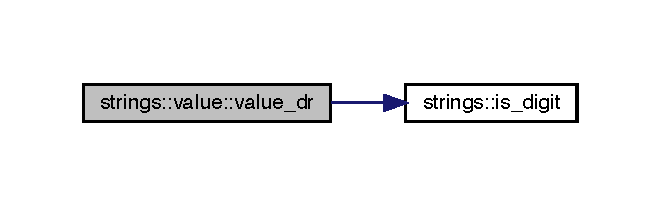
\includegraphics[width=317pt]{interfacestrings_1_1value_a8c03ca7c04583872ec5501088bea2e5b_cgraph}
\end{center}
\end{figure}
\mbox{\Hypertarget{interfacestrings_1_1value_a702d7223cac0986148075c7e9c889fb8}\label{interfacestrings_1_1value_a702d7223cac0986148075c7e9c889fb8}} 
\index{strings\+::value@{strings\+::value}!value\+\_\+si@{value\+\_\+si}}
\index{value\+\_\+si@{value\+\_\+si}!strings\+::value@{strings\+::value}}
\subsubsection{\texorpdfstring{value\+\_\+si()}{value\_si()}}
{\footnotesize\ttfamily subroutine strings\+::value\+::value\+\_\+si (\begin{DoxyParamCaption}\item[{character(len=$\ast$)}]{str,  }\item[{integer(ki4)}]{inum,  }\item[{}]{ios }\end{DoxyParamCaption})}



Definition at line 220 of file stringmod.\+f95.

\mbox{\Hypertarget{interfacestrings_1_1value_a5e6f162c9e02b46a92d20e9e65c9fc36}\label{interfacestrings_1_1value_a5e6f162c9e02b46a92d20e9e65c9fc36}} 
\index{strings\+::value@{strings\+::value}!value\+\_\+sr@{value\+\_\+sr}}
\index{value\+\_\+sr@{value\+\_\+sr}!strings\+::value@{strings\+::value}}
\subsubsection{\texorpdfstring{value\+\_\+sr()}{value\_sr()}}
{\footnotesize\ttfamily subroutine strings\+::value\+::value\+\_\+sr (\begin{DoxyParamCaption}\item[{character(len=$\ast$)}]{str,  }\item[{real(kr4)}]{rnum,  }\item[{}]{ios }\end{DoxyParamCaption})}



Definition at line 181 of file stringmod.\+f95.



The documentation for this interface was generated from the following file\+:\begin{DoxyCompactItemize}
\item 
\hyperlink{stringmod_8f95}{stringmod.\+f95}\end{DoxyCompactItemize}

\hypertarget{structctrl__output_1_1varattr}{}\section{ctrl\+\_\+output\+:\+:varattr Type Reference}
\label{structctrl__output_1_1varattr}\index{ctrl\+\_\+output\+::varattr@{ctrl\+\_\+output\+::varattr}}
\subsection*{Public Attributes}
\begin{DoxyCompactItemize}
\item 
character(len=15) \hyperlink{structctrl__output_1_1varattr_ac5d564a1b51aca6652ee5999d86ee3c5}{header}
\item 
character(len=12) \hyperlink{structctrl__output_1_1varattr_aa0d2944f6f1767e7e856831c96f4dffb}{unit}
\item 
character(len=14) \hyperlink{structctrl__output_1_1varattr_a1939d217311a5e0fb5571efdc8df0f42}{fmt}
\item 
character(len=50) \hyperlink{structctrl__output_1_1varattr_ad9c9880260734807056c2bc27806a5ec}{longnm}
\item 
character(len=1) \hyperlink{structctrl__output_1_1varattr_aa72f69bfd2f35d9815ceb0bcaf344f5c}{aggreg}
\item 
character(len=10) \hyperlink{structctrl__output_1_1varattr_af5c0a029bc5b7de926c9f771ecbaa16e}{group}
\item 
integer \hyperlink{structctrl__output_1_1varattr_a0b8734fea9cd4b6406b8faf8dc16c6d8}{level}
\end{DoxyCompactItemize}


\subsection{Detailed Description}


Definition at line 58 of file S\+U\+E\+W\+S\+\_\+ctrl\+\_\+output.\+f95.



\subsection{Member Data Documentation}
\mbox{\Hypertarget{structctrl__output_1_1varattr_aa72f69bfd2f35d9815ceb0bcaf344f5c}\label{structctrl__output_1_1varattr_aa72f69bfd2f35d9815ceb0bcaf344f5c}} 
\index{ctrl\+\_\+output\+::varattr@{ctrl\+\_\+output\+::varattr}!aggreg@{aggreg}}
\index{aggreg@{aggreg}!ctrl\+\_\+output\+::varattr@{ctrl\+\_\+output\+::varattr}}
\subsubsection{\texorpdfstring{aggreg}{aggreg}}
{\footnotesize\ttfamily character(len = 1) ctrl\+\_\+output\+::varattr\+::aggreg}



Definition at line 63 of file S\+U\+E\+W\+S\+\_\+ctrl\+\_\+output.\+f95.

\mbox{\Hypertarget{structctrl__output_1_1varattr_a1939d217311a5e0fb5571efdc8df0f42}\label{structctrl__output_1_1varattr_a1939d217311a5e0fb5571efdc8df0f42}} 
\index{ctrl\+\_\+output\+::varattr@{ctrl\+\_\+output\+::varattr}!fmt@{fmt}}
\index{fmt@{fmt}!ctrl\+\_\+output\+::varattr@{ctrl\+\_\+output\+::varattr}}
\subsubsection{\texorpdfstring{fmt}{fmt}}
{\footnotesize\ttfamily character(len = 14) ctrl\+\_\+output\+::varattr\+::fmt}



Definition at line 61 of file S\+U\+E\+W\+S\+\_\+ctrl\+\_\+output.\+f95.

\mbox{\Hypertarget{structctrl__output_1_1varattr_af5c0a029bc5b7de926c9f771ecbaa16e}\label{structctrl__output_1_1varattr_af5c0a029bc5b7de926c9f771ecbaa16e}} 
\index{ctrl\+\_\+output\+::varattr@{ctrl\+\_\+output\+::varattr}!group@{group}}
\index{group@{group}!ctrl\+\_\+output\+::varattr@{ctrl\+\_\+output\+::varattr}}
\subsubsection{\texorpdfstring{group}{group}}
{\footnotesize\ttfamily character(len = 10) ctrl\+\_\+output\+::varattr\+::group}



Definition at line 64 of file S\+U\+E\+W\+S\+\_\+ctrl\+\_\+output.\+f95.

\mbox{\Hypertarget{structctrl__output_1_1varattr_ac5d564a1b51aca6652ee5999d86ee3c5}\label{structctrl__output_1_1varattr_ac5d564a1b51aca6652ee5999d86ee3c5}} 
\index{ctrl\+\_\+output\+::varattr@{ctrl\+\_\+output\+::varattr}!header@{header}}
\index{header@{header}!ctrl\+\_\+output\+::varattr@{ctrl\+\_\+output\+::varattr}}
\subsubsection{\texorpdfstring{header}{header}}
{\footnotesize\ttfamily character(len = 15) ctrl\+\_\+output\+::varattr\+::header}



Definition at line 59 of file S\+U\+E\+W\+S\+\_\+ctrl\+\_\+output.\+f95.

\mbox{\Hypertarget{structctrl__output_1_1varattr_a0b8734fea9cd4b6406b8faf8dc16c6d8}\label{structctrl__output_1_1varattr_a0b8734fea9cd4b6406b8faf8dc16c6d8}} 
\index{ctrl\+\_\+output\+::varattr@{ctrl\+\_\+output\+::varattr}!level@{level}}
\index{level@{level}!ctrl\+\_\+output\+::varattr@{ctrl\+\_\+output\+::varattr}}
\subsubsection{\texorpdfstring{level}{level}}
{\footnotesize\ttfamily integer ctrl\+\_\+output\+::varattr\+::level}



Definition at line 65 of file S\+U\+E\+W\+S\+\_\+ctrl\+\_\+output.\+f95.

\mbox{\Hypertarget{structctrl__output_1_1varattr_ad9c9880260734807056c2bc27806a5ec}\label{structctrl__output_1_1varattr_ad9c9880260734807056c2bc27806a5ec}} 
\index{ctrl\+\_\+output\+::varattr@{ctrl\+\_\+output\+::varattr}!longnm@{longnm}}
\index{longnm@{longnm}!ctrl\+\_\+output\+::varattr@{ctrl\+\_\+output\+::varattr}}
\subsubsection{\texorpdfstring{longnm}{longnm}}
{\footnotesize\ttfamily character(len = 50) ctrl\+\_\+output\+::varattr\+::longnm}



Definition at line 62 of file S\+U\+E\+W\+S\+\_\+ctrl\+\_\+output.\+f95.

\mbox{\Hypertarget{structctrl__output_1_1varattr_aa0d2944f6f1767e7e856831c96f4dffb}\label{structctrl__output_1_1varattr_aa0d2944f6f1767e7e856831c96f4dffb}} 
\index{ctrl\+\_\+output\+::varattr@{ctrl\+\_\+output\+::varattr}!unit@{unit}}
\index{unit@{unit}!ctrl\+\_\+output\+::varattr@{ctrl\+\_\+output\+::varattr}}
\subsubsection{\texorpdfstring{unit}{unit}}
{\footnotesize\ttfamily character(len = 12) ctrl\+\_\+output\+::varattr\+::unit}



Definition at line 60 of file S\+U\+E\+W\+S\+\_\+ctrl\+\_\+output.\+f95.



The documentation for this type was generated from the following file\+:\begin{DoxyCompactItemize}
\item 
\hyperlink{_s_u_e_w_s__ctrl__output_8f95}{S\+U\+E\+W\+S\+\_\+ctrl\+\_\+output.\+f95}\end{DoxyCompactItemize}

\hypertarget{interfacestrings_1_1writenum}{}\section{strings\+:\+:writenum Interface Reference}
\label{interfacestrings_1_1writenum}\index{strings\+::writenum@{strings\+::writenum}}
\subsection*{Public Member Functions}
\begin{DoxyCompactItemize}
\item 
subroutine \hyperlink{interfacestrings_1_1writenum_a41519a1d4a27d51318cbdbd6c02ada41}{write\+\_\+dr} (rnum, \hyperlink{_s_o_l_w_e_i_g__misc_8f95_a77a2ca74046c88062aa8333bf1eaca05}{str}, fmt)
\item 
subroutine \hyperlink{interfacestrings_1_1writenum_a057712cfbe8449b5c0f9ccb80a50c68e}{write\+\_\+sr} (rnum, \hyperlink{_s_o_l_w_e_i_g__misc_8f95_a77a2ca74046c88062aa8333bf1eaca05}{str}, fmt)
\item 
subroutine \hyperlink{interfacestrings_1_1writenum_a23cc22768358f32dca2eca631aca318d}{write\+\_\+di} (inum, \hyperlink{_s_o_l_w_e_i_g__misc_8f95_a77a2ca74046c88062aa8333bf1eaca05}{str}, fmt)
\item 
subroutine \hyperlink{interfacestrings_1_1writenum_a7cd46c3fce679fe99b15b5f38cda22c5}{write\+\_\+si} (inum, \hyperlink{_s_o_l_w_e_i_g__misc_8f95_a77a2ca74046c88062aa8333bf1eaca05}{str}, fmt)
\end{DoxyCompactItemize}


\subsection{Detailed Description}


Definition at line 21 of file stringmod.\+f95.



\subsection{Member Function/\+Subroutine Documentation}
\mbox{\Hypertarget{interfacestrings_1_1writenum_a23cc22768358f32dca2eca631aca318d}\label{interfacestrings_1_1writenum_a23cc22768358f32dca2eca631aca318d}} 
\index{strings\+::writenum@{strings\+::writenum}!write\+\_\+di@{write\+\_\+di}}
\index{write\+\_\+di@{write\+\_\+di}!strings\+::writenum@{strings\+::writenum}}
\subsubsection{\texorpdfstring{write\+\_\+di()}{write\_di()}}
{\footnotesize\ttfamily subroutine strings\+::writenum\+::write\+\_\+di (\begin{DoxyParamCaption}\item[{integer(ki8)}]{inum,  }\item[{character(len=$\ast$)}]{str,  }\item[{character(len=$\ast$)}]{fmt }\end{DoxyParamCaption})}



Definition at line 513 of file stringmod.\+f95.

\mbox{\Hypertarget{interfacestrings_1_1writenum_a41519a1d4a27d51318cbdbd6c02ada41}\label{interfacestrings_1_1writenum_a41519a1d4a27d51318cbdbd6c02ada41}} 
\index{strings\+::writenum@{strings\+::writenum}!write\+\_\+dr@{write\+\_\+dr}}
\index{write\+\_\+dr@{write\+\_\+dr}!strings\+::writenum@{strings\+::writenum}}
\subsubsection{\texorpdfstring{write\+\_\+dr()}{write\_dr()}}
{\footnotesize\ttfamily subroutine strings\+::writenum\+::write\+\_\+dr (\begin{DoxyParamCaption}\item[{real(kr8)}]{rnum,  }\item[{character(len=$\ast$)}]{str,  }\item[{character(len=$\ast$)}]{fmt }\end{DoxyParamCaption})}



Definition at line 481 of file stringmod.\+f95.

\mbox{\Hypertarget{interfacestrings_1_1writenum_a7cd46c3fce679fe99b15b5f38cda22c5}\label{interfacestrings_1_1writenum_a7cd46c3fce679fe99b15b5f38cda22c5}} 
\index{strings\+::writenum@{strings\+::writenum}!write\+\_\+si@{write\+\_\+si}}
\index{write\+\_\+si@{write\+\_\+si}!strings\+::writenum@{strings\+::writenum}}
\subsubsection{\texorpdfstring{write\+\_\+si()}{write\_si()}}
{\footnotesize\ttfamily subroutine strings\+::writenum\+::write\+\_\+si (\begin{DoxyParamCaption}\item[{integer(ki4)}]{inum,  }\item[{character(len=$\ast$)}]{str,  }\item[{character(len=$\ast$)}]{fmt }\end{DoxyParamCaption})}



Definition at line 529 of file stringmod.\+f95.

\mbox{\Hypertarget{interfacestrings_1_1writenum_a057712cfbe8449b5c0f9ccb80a50c68e}\label{interfacestrings_1_1writenum_a057712cfbe8449b5c0f9ccb80a50c68e}} 
\index{strings\+::writenum@{strings\+::writenum}!write\+\_\+sr@{write\+\_\+sr}}
\index{write\+\_\+sr@{write\+\_\+sr}!strings\+::writenum@{strings\+::writenum}}
\subsubsection{\texorpdfstring{write\+\_\+sr()}{write\_sr()}}
{\footnotesize\ttfamily subroutine strings\+::writenum\+::write\+\_\+sr (\begin{DoxyParamCaption}\item[{real(kr4)}]{rnum,  }\item[{character(len=$\ast$)}]{str,  }\item[{character(len=$\ast$)}]{fmt }\end{DoxyParamCaption})}



Definition at line 497 of file stringmod.\+f95.



The documentation for this interface was generated from the following file\+:\begin{DoxyCompactItemize}
\item 
\hyperlink{stringmod_8f95}{stringmod.\+f95}\end{DoxyCompactItemize}

\hypertarget{interfacestrings_1_1writeq}{}\section{strings\+:\+:writeq Interface Reference}
\label{interfacestrings_1_1writeq}\index{strings\+::writeq@{strings\+::writeq}}
\subsection*{Public Member Functions}
\begin{DoxyCompactItemize}
\item 
subroutine \hyperlink{interfacestrings_1_1writeq_a141904a2ffb98125035f6ce0944ffd4c}{writeq\+\_\+dr} (unit, namestr, \hyperlink{interfacestrings_1_1value}{value}, fmt)
\item 
subroutine \hyperlink{interfacestrings_1_1writeq_a2c9743fd678c7eb3387f7acae35de200}{writeq\+\_\+sr} (unit, namestr, \hyperlink{interfacestrings_1_1value}{value}, fmt)
\item 
subroutine \hyperlink{interfacestrings_1_1writeq_a19d50dea30fcb08479b3ec0626c58f69}{writeq\+\_\+di} (unit, namestr, ivalue, fmt)
\item 
subroutine \hyperlink{interfacestrings_1_1writeq_af7f414c54607f15965a0e67c7702aa9c}{writeq\+\_\+si} (unit, namestr, ivalue, fmt)
\end{DoxyCompactItemize}


\subsection{Detailed Description}


Definition at line 33 of file stringmod.\+f95.



\subsection{Member Function/\+Subroutine Documentation}
\mbox{\Hypertarget{interfacestrings_1_1writeq_a19d50dea30fcb08479b3ec0626c58f69}\label{interfacestrings_1_1writeq_a19d50dea30fcb08479b3ec0626c58f69}} 
\index{strings\+::writeq@{strings\+::writeq}!writeq\+\_\+di@{writeq\+\_\+di}}
\index{writeq\+\_\+di@{writeq\+\_\+di}!strings\+::writeq@{strings\+::writeq}}
\subsubsection{\texorpdfstring{writeq\+\_\+di()}{writeq\_di()}}
{\footnotesize\ttfamily subroutine strings\+::writeq\+::writeq\+\_\+di (\begin{DoxyParamCaption}\item[{integer}]{unit,  }\item[{character(len=$\ast$)}]{namestr,  }\item[{integer(ki8)}]{ivalue,  }\item[{character(len=$\ast$)}]{fmt }\end{DoxyParamCaption})}



Definition at line 611 of file stringmod.\+f95.

Here is the call graph for this function\+:\nopagebreak
\begin{figure}[H]
\begin{center}
\leavevmode
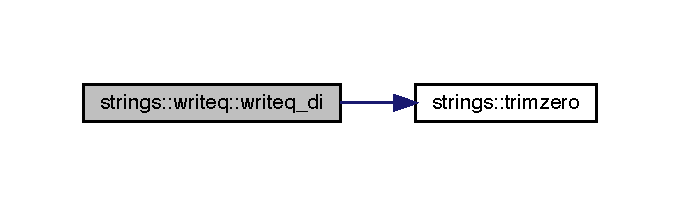
\includegraphics[width=326pt]{interfacestrings_1_1writeq_a19d50dea30fcb08479b3ec0626c58f69_cgraph}
\end{center}
\end{figure}
\mbox{\Hypertarget{interfacestrings_1_1writeq_a141904a2ffb98125035f6ce0944ffd4c}\label{interfacestrings_1_1writeq_a141904a2ffb98125035f6ce0944ffd4c}} 
\index{strings\+::writeq@{strings\+::writeq}!writeq\+\_\+dr@{writeq\+\_\+dr}}
\index{writeq\+\_\+dr@{writeq\+\_\+dr}!strings\+::writeq@{strings\+::writeq}}
\subsubsection{\texorpdfstring{writeq\+\_\+dr()}{writeq\_dr()}}
{\footnotesize\ttfamily subroutine strings\+::writeq\+::writeq\+\_\+dr (\begin{DoxyParamCaption}\item[{integer}]{unit,  }\item[{character(len=$\ast$)}]{namestr,  }\item[{real(kr8)}]{value,  }\item[{character(len=$\ast$)}]{fmt }\end{DoxyParamCaption})}



Definition at line 577 of file stringmod.\+f95.

Here is the call graph for this function\+:\nopagebreak
\begin{figure}[H]
\begin{center}
\leavevmode
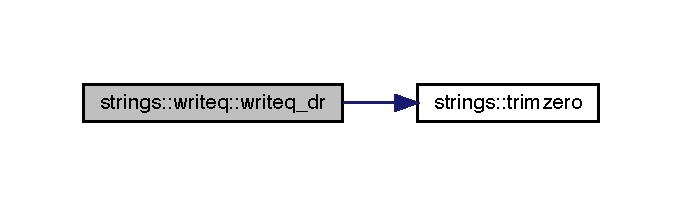
\includegraphics[width=327pt]{interfacestrings_1_1writeq_a141904a2ffb98125035f6ce0944ffd4c_cgraph}
\end{center}
\end{figure}
\mbox{\Hypertarget{interfacestrings_1_1writeq_af7f414c54607f15965a0e67c7702aa9c}\label{interfacestrings_1_1writeq_af7f414c54607f15965a0e67c7702aa9c}} 
\index{strings\+::writeq@{strings\+::writeq}!writeq\+\_\+si@{writeq\+\_\+si}}
\index{writeq\+\_\+si@{writeq\+\_\+si}!strings\+::writeq@{strings\+::writeq}}
\subsubsection{\texorpdfstring{writeq\+\_\+si()}{writeq\_si()}}
{\footnotesize\ttfamily subroutine strings\+::writeq\+::writeq\+\_\+si (\begin{DoxyParamCaption}\item[{integer}]{unit,  }\item[{character(len=$\ast$)}]{namestr,  }\item[{integer(ki4)}]{ivalue,  }\item[{character(len=$\ast$)}]{fmt }\end{DoxyParamCaption})}



Definition at line 627 of file stringmod.\+f95.

Here is the call graph for this function\+:\nopagebreak
\begin{figure}[H]
\begin{center}
\leavevmode
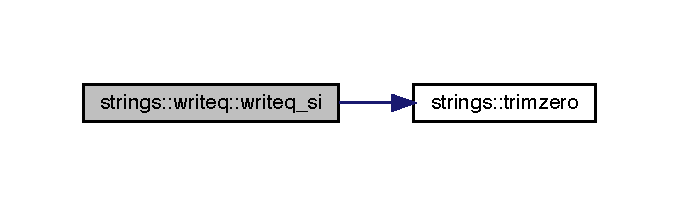
\includegraphics[width=326pt]{interfacestrings_1_1writeq_af7f414c54607f15965a0e67c7702aa9c_cgraph}
\end{center}
\end{figure}
\mbox{\Hypertarget{interfacestrings_1_1writeq_a2c9743fd678c7eb3387f7acae35de200}\label{interfacestrings_1_1writeq_a2c9743fd678c7eb3387f7acae35de200}} 
\index{strings\+::writeq@{strings\+::writeq}!writeq\+\_\+sr@{writeq\+\_\+sr}}
\index{writeq\+\_\+sr@{writeq\+\_\+sr}!strings\+::writeq@{strings\+::writeq}}
\subsubsection{\texorpdfstring{writeq\+\_\+sr()}{writeq\_sr()}}
{\footnotesize\ttfamily subroutine strings\+::writeq\+::writeq\+\_\+sr (\begin{DoxyParamCaption}\item[{integer}]{unit,  }\item[{character(len=$\ast$)}]{namestr,  }\item[{real(kr4)}]{value,  }\item[{character(len=$\ast$)}]{fmt }\end{DoxyParamCaption})}



Definition at line 594 of file stringmod.\+f95.

Here is the call graph for this function\+:\nopagebreak
\begin{figure}[H]
\begin{center}
\leavevmode
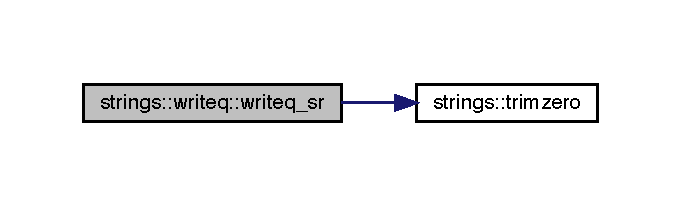
\includegraphics[width=327pt]{interfacestrings_1_1writeq_a2c9743fd678c7eb3387f7acae35de200_cgraph}
\end{center}
\end{figure}


The documentation for this interface was generated from the following file\+:\begin{DoxyCompactItemize}
\item 
\hyperlink{stringmod_8f95}{stringmod.\+f95}\end{DoxyCompactItemize}

\chapter{File Documentation}
\hypertarget{_b_l_u_e_w_s___c_b_l_8f95}{}\section{B\+L\+U\+E\+W\+S\+\_\+\+C\+B\+L.\+f95 File Reference}
\label{_b_l_u_e_w_s___c_b_l_8f95}\index{B\+L\+U\+E\+W\+S\+\_\+\+C\+B\+L.\+f95@{B\+L\+U\+E\+W\+S\+\_\+\+C\+B\+L.\+f95}}
\subsection*{Functions/\+Subroutines}
\begin{DoxyCompactItemize}
\item 
subroutine \hyperlink{_b_l_u_e_w_s___c_b_l_8f95_acde23a276c692f0ec2a493dc9720471c}{cbl} (ifirst, i\+MB, Gridiv)
\item 
subroutine \hyperlink{_b_l_u_e_w_s___c_b_l_8f95_a2b7c9b5778366f3415268e6939cab229}{cbl\+\_\+readinputdata}
\item 
subroutine \hyperlink{_b_l_u_e_w_s___c_b_l_8f95_a2070c594a28f66b5ee4b95cd0251621e}{cbl\+\_\+initial} (qh\+\_\+use, qe\+\_\+use, tm\+\_\+\+K\+\_\+zm, qm\+\_\+gkg\+\_\+zm, startflag, i\+MB, Gridiv)
\item 
subroutine \hyperlink{_b_l_u_e_w_s___c_b_l_8f95_ada6e5e5cd6b578659b196bb8c26bd98c}{nbl} (qh\+\_\+use, qe\+\_\+use, tm\+\_\+\+K\+\_\+zm, qm\+\_\+gkg\+\_\+zm, startflag, i\+Mb, Gridiv)
\item 
real(kind(1d0)) function \hyperlink{_b_l_u_e_w_s___c_b_l_8f95_a67036afb2f40fef682aefc6df6d0c311}{qsatf} (T, P\+MB)
\end{DoxyCompactItemize}


\subsection{Function/\+Subroutine Documentation}
\mbox{\Hypertarget{_b_l_u_e_w_s___c_b_l_8f95_acde23a276c692f0ec2a493dc9720471c}\label{_b_l_u_e_w_s___c_b_l_8f95_acde23a276c692f0ec2a493dc9720471c}} 
\index{B\+L\+U\+E\+W\+S\+\_\+\+C\+B\+L.\+f95@{B\+L\+U\+E\+W\+S\+\_\+\+C\+B\+L.\+f95}!cbl@{cbl}}
\index{cbl@{cbl}!B\+L\+U\+E\+W\+S\+\_\+\+C\+B\+L.\+f95@{B\+L\+U\+E\+W\+S\+\_\+\+C\+B\+L.\+f95}}
\subsubsection{\texorpdfstring{cbl()}{cbl()}}
{\footnotesize\ttfamily subroutine cbl (\begin{DoxyParamCaption}\item[{integer}]{ifirst,  }\item[{integer}]{i\+MB,  }\item[{integer}]{Gridiv }\end{DoxyParamCaption})}



Definition at line 9 of file B\+L\+U\+E\+W\+S\+\_\+\+C\+B\+L.\+f95.

Here is the call graph for this function\+:\nopagebreak
\begin{figure}[H]
\begin{center}
\leavevmode
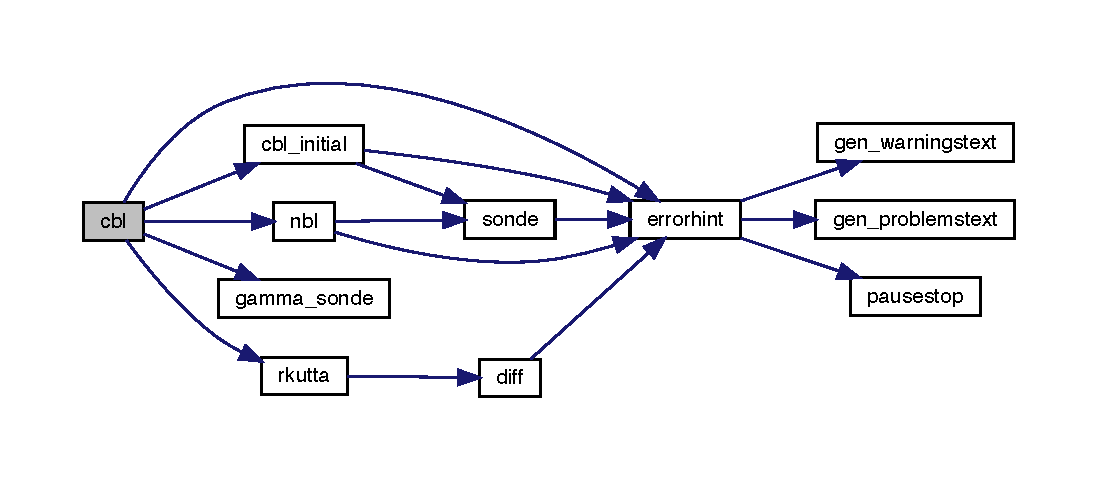
\includegraphics[width=350pt]{_b_l_u_e_w_s___c_b_l_8f95_acde23a276c692f0ec2a493dc9720471c_cgraph}
\end{center}
\end{figure}
\mbox{\Hypertarget{_b_l_u_e_w_s___c_b_l_8f95_a2070c594a28f66b5ee4b95cd0251621e}\label{_b_l_u_e_w_s___c_b_l_8f95_a2070c594a28f66b5ee4b95cd0251621e}} 
\index{B\+L\+U\+E\+W\+S\+\_\+\+C\+B\+L.\+f95@{B\+L\+U\+E\+W\+S\+\_\+\+C\+B\+L.\+f95}!cbl\+\_\+initial@{cbl\+\_\+initial}}
\index{cbl\+\_\+initial@{cbl\+\_\+initial}!B\+L\+U\+E\+W\+S\+\_\+\+C\+B\+L.\+f95@{B\+L\+U\+E\+W\+S\+\_\+\+C\+B\+L.\+f95}}
\subsubsection{\texorpdfstring{cbl\+\_\+initial()}{cbl\_initial()}}
{\footnotesize\ttfamily subroutine cbl\+\_\+initial (\begin{DoxyParamCaption}\item[{real(kind(1d0))}]{qh\+\_\+use,  }\item[{real(kind(1d0))}]{qe\+\_\+use,  }\item[{real(kind(1d0))}]{tm\+\_\+\+K\+\_\+zm,  }\item[{real(kind(1d0))}]{qm\+\_\+gkg\+\_\+zm,  }\item[{integer}]{startflag,  }\item[{integer}]{i\+MB,  }\item[{integer}]{Gridiv }\end{DoxyParamCaption})}



Definition at line 277 of file B\+L\+U\+E\+W\+S\+\_\+\+C\+B\+L.\+f95.

Here is the call graph for this function\+:\nopagebreak
\begin{figure}[H]
\begin{center}
\leavevmode
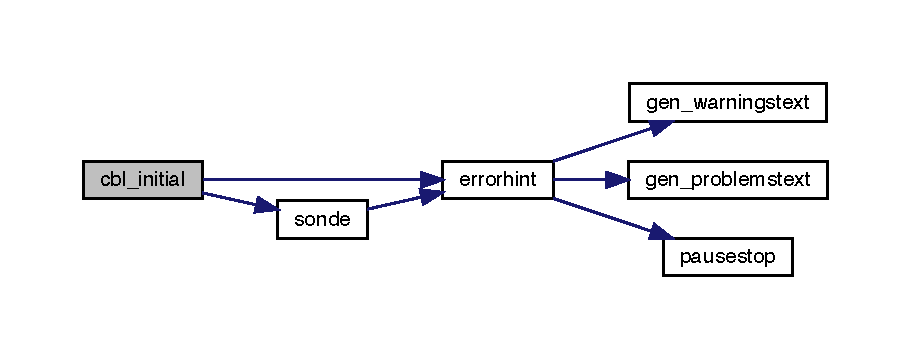
\includegraphics[width=350pt]{_b_l_u_e_w_s___c_b_l_8f95_a2070c594a28f66b5ee4b95cd0251621e_cgraph}
\end{center}
\end{figure}
\mbox{\Hypertarget{_b_l_u_e_w_s___c_b_l_8f95_a2b7c9b5778366f3415268e6939cab229}\label{_b_l_u_e_w_s___c_b_l_8f95_a2b7c9b5778366f3415268e6939cab229}} 
\index{B\+L\+U\+E\+W\+S\+\_\+\+C\+B\+L.\+f95@{B\+L\+U\+E\+W\+S\+\_\+\+C\+B\+L.\+f95}!cbl\+\_\+readinputdata@{cbl\+\_\+readinputdata}}
\index{cbl\+\_\+readinputdata@{cbl\+\_\+readinputdata}!B\+L\+U\+E\+W\+S\+\_\+\+C\+B\+L.\+f95@{B\+L\+U\+E\+W\+S\+\_\+\+C\+B\+L.\+f95}}
\subsubsection{\texorpdfstring{cbl\+\_\+readinputdata()}{cbl\_readinputdata()}}
{\footnotesize\ttfamily subroutine cbl\+\_\+readinputdata (\begin{DoxyParamCaption}{ }\end{DoxyParamCaption})}



Definition at line 212 of file B\+L\+U\+E\+W\+S\+\_\+\+C\+B\+L.\+f95.

Here is the call graph for this function\+:\nopagebreak
\begin{figure}[H]
\begin{center}
\leavevmode
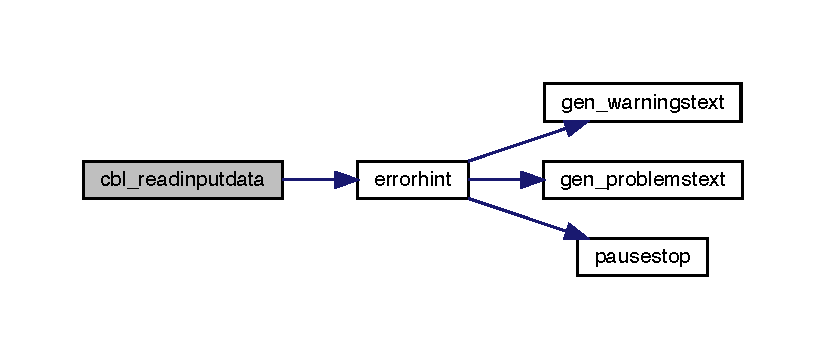
\includegraphics[width=350pt]{_b_l_u_e_w_s___c_b_l_8f95_a2b7c9b5778366f3415268e6939cab229_cgraph}
\end{center}
\end{figure}
\mbox{\Hypertarget{_b_l_u_e_w_s___c_b_l_8f95_ada6e5e5cd6b578659b196bb8c26bd98c}\label{_b_l_u_e_w_s___c_b_l_8f95_ada6e5e5cd6b578659b196bb8c26bd98c}} 
\index{B\+L\+U\+E\+W\+S\+\_\+\+C\+B\+L.\+f95@{B\+L\+U\+E\+W\+S\+\_\+\+C\+B\+L.\+f95}!nbl@{nbl}}
\index{nbl@{nbl}!B\+L\+U\+E\+W\+S\+\_\+\+C\+B\+L.\+f95@{B\+L\+U\+E\+W\+S\+\_\+\+C\+B\+L.\+f95}}
\subsubsection{\texorpdfstring{nbl()}{nbl()}}
{\footnotesize\ttfamily subroutine nbl (\begin{DoxyParamCaption}\item[{real(kind(1d0))}]{qh\+\_\+use,  }\item[{real(kind(1d0))}]{qe\+\_\+use,  }\item[{real(kind(1d0))}]{tm\+\_\+\+K\+\_\+zm,  }\item[{real(kind(1d0))}]{qm\+\_\+gkg\+\_\+zm,  }\item[{integer}]{startflag,  }\item[{integer}]{i\+Mb,  }\item[{integer}]{Gridiv }\end{DoxyParamCaption})}



Definition at line 401 of file B\+L\+U\+E\+W\+S\+\_\+\+C\+B\+L.\+f95.

Here is the call graph for this function\+:\nopagebreak
\begin{figure}[H]
\begin{center}
\leavevmode
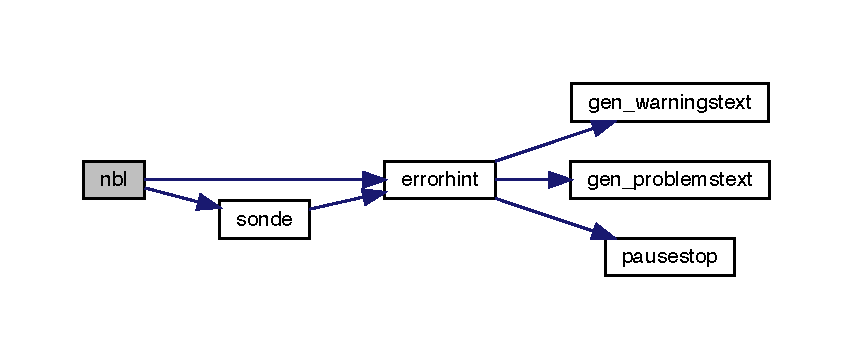
\includegraphics[width=350pt]{_b_l_u_e_w_s___c_b_l_8f95_ada6e5e5cd6b578659b196bb8c26bd98c_cgraph}
\end{center}
\end{figure}
\mbox{\Hypertarget{_b_l_u_e_w_s___c_b_l_8f95_a67036afb2f40fef682aefc6df6d0c311}\label{_b_l_u_e_w_s___c_b_l_8f95_a67036afb2f40fef682aefc6df6d0c311}} 
\index{B\+L\+U\+E\+W\+S\+\_\+\+C\+B\+L.\+f95@{B\+L\+U\+E\+W\+S\+\_\+\+C\+B\+L.\+f95}!qsatf@{qsatf}}
\index{qsatf@{qsatf}!B\+L\+U\+E\+W\+S\+\_\+\+C\+B\+L.\+f95@{B\+L\+U\+E\+W\+S\+\_\+\+C\+B\+L.\+f95}}
\subsubsection{\texorpdfstring{qsatf()}{qsatf()}}
{\footnotesize\ttfamily real (kind(1d0)) function qsatf (\begin{DoxyParamCaption}\item[{real (kind(1d0))}]{T,  }\item[{real (kind(1d0))}]{P\+MB }\end{DoxyParamCaption})}



Definition at line 538 of file B\+L\+U\+E\+W\+S\+\_\+\+C\+B\+L.\+f95.

Here is the call graph for this function\+:\nopagebreak
\begin{figure}[H]
\begin{center}
\leavevmode
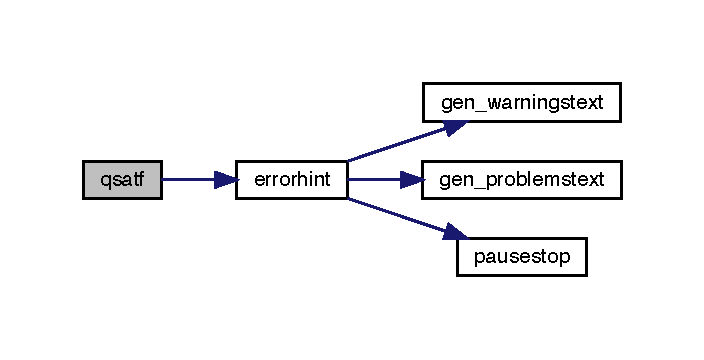
\includegraphics[width=338pt]{_b_l_u_e_w_s___c_b_l_8f95_a67036afb2f40fef682aefc6df6d0c311_cgraph}
\end{center}
\end{figure}

\hypertarget{_b_l_u_e_w_s___diff_8f95}{}\section{B\+L\+U\+E\+W\+S\+\_\+\+Diff.\+f95 File Reference}
\label{_b_l_u_e_w_s___diff_8f95}\index{B\+L\+U\+E\+W\+S\+\_\+\+Diff.\+f95@{B\+L\+U\+E\+W\+S\+\_\+\+Diff.\+f95}}
\subsection*{Functions/\+Subroutines}
\begin{DoxyCompactItemize}
\item 
subroutine \hyperlink{_b_l_u_e_w_s___diff_8f95_aa6b01ddf379446848f8a822a7918fcd0}{rkutta} (neqn, XA, XB, Y, N\+S\+T\+E\+PS)
\item 
subroutine \hyperlink{_b_l_u_e_w_s___diff_8f95_ac594a7935b340caab469006de9da9358}{diff} (s, y1, dyds)
\item 
subroutine \hyperlink{_b_l_u_e_w_s___diff_8f95_a63eab50bdd789005154d787035910277}{sonde} (id)
\item 
subroutine \hyperlink{_b_l_u_e_w_s___diff_8f95_a27fc32bfb9bfb2d6e21511c2e8c9bfed}{gamma\+\_\+sonde}
\end{DoxyCompactItemize}


\subsection{Function/\+Subroutine Documentation}
\mbox{\Hypertarget{_b_l_u_e_w_s___diff_8f95_ac594a7935b340caab469006de9da9358}\label{_b_l_u_e_w_s___diff_8f95_ac594a7935b340caab469006de9da9358}} 
\index{B\+L\+U\+E\+W\+S\+\_\+\+Diff.\+f95@{B\+L\+U\+E\+W\+S\+\_\+\+Diff.\+f95}!diff@{diff}}
\index{diff@{diff}!B\+L\+U\+E\+W\+S\+\_\+\+Diff.\+f95@{B\+L\+U\+E\+W\+S\+\_\+\+Diff.\+f95}}
\subsubsection{\texorpdfstring{diff()}{diff()}}
{\footnotesize\ttfamily subroutine diff (\begin{DoxyParamCaption}\item[{real(kind(1d0))}]{s,  }\item[{real(kind(1d0)), dimension(neqn)}]{y1,  }\item[{real(kind(1d0)), dimension(neqn)}]{dyds }\end{DoxyParamCaption})}



Definition at line 84 of file B\+L\+U\+E\+W\+S\+\_\+\+Diff.\+f95.

Here is the call graph for this function\+:\nopagebreak
\begin{figure}[H]
\begin{center}
\leavevmode
\includegraphics[width=330pt]{_b_l_u_e_w_s___diff_8f95_ac594a7935b340caab469006de9da9358_cgraph}
\end{center}
\end{figure}
\mbox{\Hypertarget{_b_l_u_e_w_s___diff_8f95_a27fc32bfb9bfb2d6e21511c2e8c9bfed}\label{_b_l_u_e_w_s___diff_8f95_a27fc32bfb9bfb2d6e21511c2e8c9bfed}} 
\index{B\+L\+U\+E\+W\+S\+\_\+\+Diff.\+f95@{B\+L\+U\+E\+W\+S\+\_\+\+Diff.\+f95}!gamma\+\_\+sonde@{gamma\+\_\+sonde}}
\index{gamma\+\_\+sonde@{gamma\+\_\+sonde}!B\+L\+U\+E\+W\+S\+\_\+\+Diff.\+f95@{B\+L\+U\+E\+W\+S\+\_\+\+Diff.\+f95}}
\subsubsection{\texorpdfstring{gamma\+\_\+sonde()}{gamma\_sonde()}}
{\footnotesize\ttfamily subroutine gamma\+\_\+sonde (\begin{DoxyParamCaption}{ }\end{DoxyParamCaption})}



Definition at line 263 of file B\+L\+U\+E\+W\+S\+\_\+\+Diff.\+f95.

\mbox{\Hypertarget{_b_l_u_e_w_s___diff_8f95_aa6b01ddf379446848f8a822a7918fcd0}\label{_b_l_u_e_w_s___diff_8f95_aa6b01ddf379446848f8a822a7918fcd0}} 
\index{B\+L\+U\+E\+W\+S\+\_\+\+Diff.\+f95@{B\+L\+U\+E\+W\+S\+\_\+\+Diff.\+f95}!rkutta@{rkutta}}
\index{rkutta@{rkutta}!B\+L\+U\+E\+W\+S\+\_\+\+Diff.\+f95@{B\+L\+U\+E\+W\+S\+\_\+\+Diff.\+f95}}
\subsubsection{\texorpdfstring{rkutta()}{rkutta()}}
{\footnotesize\ttfamily subroutine rkutta (\begin{DoxyParamCaption}\item[{integer}]{neqn,  }\item[{real (kind(1d0))}]{XA,  }\item[{real (kind(1d0))}]{XB,  }\item[{real(kind(1d0)), dimension (neqn)}]{Y,  }\item[{integer}]{N\+S\+T\+E\+PS }\end{DoxyParamCaption})}



Definition at line 7 of file B\+L\+U\+E\+W\+S\+\_\+\+Diff.\+f95.

Here is the call graph for this function\+:\nopagebreak
\begin{figure}[H]
\begin{center}
\leavevmode
\includegraphics[width=350pt]{_b_l_u_e_w_s___diff_8f95_aa6b01ddf379446848f8a822a7918fcd0_cgraph}
\end{center}
\end{figure}
\mbox{\Hypertarget{_b_l_u_e_w_s___diff_8f95_a63eab50bdd789005154d787035910277}\label{_b_l_u_e_w_s___diff_8f95_a63eab50bdd789005154d787035910277}} 
\index{B\+L\+U\+E\+W\+S\+\_\+\+Diff.\+f95@{B\+L\+U\+E\+W\+S\+\_\+\+Diff.\+f95}!sonde@{sonde}}
\index{sonde@{sonde}!B\+L\+U\+E\+W\+S\+\_\+\+Diff.\+f95@{B\+L\+U\+E\+W\+S\+\_\+\+Diff.\+f95}}
\subsubsection{\texorpdfstring{sonde()}{sonde()}}
{\footnotesize\ttfamily subroutine sonde (\begin{DoxyParamCaption}\item[{integer}]{id }\end{DoxyParamCaption})}



Definition at line 229 of file B\+L\+U\+E\+W\+S\+\_\+\+Diff.\+f95.

Here is the call graph for this function\+:\nopagebreak
\begin{figure}[H]
\begin{center}
\leavevmode
\includegraphics[width=344pt]{_b_l_u_e_w_s___diff_8f95_a63eab50bdd789005154d787035910277_cgraph}
\end{center}
\end{figure}

\hypertarget{_l_u_m_p_s__atmos__functions__moist_8f95}{}\section{L\+U\+M\+P\+S\+\_\+atmos\+\_\+functions\+\_\+moist.\+f95 File Reference}
\label{_l_u_m_p_s__atmos__functions__moist_8f95}\index{L\+U\+M\+P\+S\+\_\+atmos\+\_\+functions\+\_\+moist.\+f95@{L\+U\+M\+P\+S\+\_\+atmos\+\_\+functions\+\_\+moist.\+f95}}
\subsection*{Functions/\+Subroutines}
\begin{DoxyCompactItemize}
\item 
subroutine \hyperlink{_l_u_m_p_s__atmos__functions__moist_8f95_ae6aae41b4a8fe866a54025d8fbc439d2}{atmos\+\_\+moist\+\_\+lumps} (Temp\+\_\+C, Press\+\_\+h\+Pa, av\+Rh, dectime, lv\+\_\+\+J\+\_\+kg, lv\+S\+\_\+\+J\+\_\+kg, es\+\_\+h\+Pa, Ea\+\_\+h\+Pa, V\+Pd\+\_\+hpa, V\+P\+D\+\_\+\+Pa, dq, dens\+\_\+dry, avcp, air\+\_\+dens)
\item 
real(kind(1d0)) function \hyperlink{_l_u_m_p_s__atmos__functions__moist_8f95_a634f4cc5a636b7b311a16a1eb64e133e}{sat\+\_\+vap\+\_\+press} (Temp\+\_\+c, P\+R\+E\+S\+S\+\_\+h\+Pa, from, dectime)
\item 
real(kind(1d0)) function \hyperlink{_l_u_m_p_s__atmos__functions__moist_8f95_a8e723cdd557d577e5e646808dc572dc1}{sat\+\_\+vap\+\_\+pressice} (Temp\+\_\+c, P\+R\+E\+S\+S\+\_\+h\+Pa, from, dectime)
\item 
real(kind(1d0)) function \hyperlink{_l_u_m_p_s__atmos__functions__moist_8f95_a23dfe0352f06dab2858ae44f81b54a89}{spec\+\_\+hum\+\_\+def} (vpd\+\_\+h\+Pa, press\+\_\+h\+Pa)
\item 
real(kind(1d0)) function \hyperlink{_l_u_m_p_s__atmos__functions__moist_8f95_ad67fce32939b8349b7af6a3aa30d2d5b}{spec\+\_\+heat\+\_\+beer} (Temp\+\_\+C, rh, rho\+\_\+v, rho\+\_\+d)
\item 
real(kind(1d0)) function \hyperlink{_l_u_m_p_s__atmos__functions__moist_8f95_a8101e1e156dd288914e76a4dccb1a08d}{lat\+\_\+vap} (Temp\+\_\+C, Ea\+\_\+h\+Pa, Press\+\_\+h\+Pa, cp, dectime)
\item 
real(kind(1d0)) function \hyperlink{_l_u_m_p_s__atmos__functions__moist_8f95_ab3e9a8945e4ba8d534a51c3df7aa7948}{lat\+\_\+vapsublim} (Temp\+\_\+C, Ea\+\_\+h\+Pa, Press\+\_\+h\+Pa, cp, dectime)
\item 
real(kind(1d0)) function \hyperlink{_l_u_m_p_s__atmos__functions__moist_8f95_aca3cbb873a6638e6d630d35e0133d1dc}{psyc\+\_\+const} (cp, Press\+\_\+h\+Pa, lv\+\_\+\+J\+\_\+kg)
\item 
real(kind(1d0)) function \hyperlink{_l_u_m_p_s__atmos__functions__moist_8f95_afee63d3fd27358ee600477b7e71802ca}{dewpoint} (ea\+\_\+h\+Pa)
\item 
real(kind(1d0)) function \hyperlink{_l_u_m_p_s__atmos__functions__moist_8f95_ad8313c7c7528e6b2fad62cfa62efc4eb}{slope\+\_\+svp} (temp\+\_\+C)
\item 
real(kind(1d0)) function \hyperlink{_l_u_m_p_s__atmos__functions__moist_8f95_a80c8af865285c09ca0cc2de78ec85cb9}{slopeice\+\_\+svp} (temp\+\_\+C)
\end{DoxyCompactItemize}


\subsection{Function/\+Subroutine Documentation}
\mbox{\Hypertarget{_l_u_m_p_s__atmos__functions__moist_8f95_ae6aae41b4a8fe866a54025d8fbc439d2}\label{_l_u_m_p_s__atmos__functions__moist_8f95_ae6aae41b4a8fe866a54025d8fbc439d2}} 
\index{L\+U\+M\+P\+S\+\_\+atmos\+\_\+functions\+\_\+moist.\+f95@{L\+U\+M\+P\+S\+\_\+atmos\+\_\+functions\+\_\+moist.\+f95}!atmos\+\_\+moist\+\_\+lumps@{atmos\+\_\+moist\+\_\+lumps}}
\index{atmos\+\_\+moist\+\_\+lumps@{atmos\+\_\+moist\+\_\+lumps}!L\+U\+M\+P\+S\+\_\+atmos\+\_\+functions\+\_\+moist.\+f95@{L\+U\+M\+P\+S\+\_\+atmos\+\_\+functions\+\_\+moist.\+f95}}
\subsubsection{\texorpdfstring{atmos\+\_\+moist\+\_\+lumps()}{atmos\_moist\_lumps()}}
{\footnotesize\ttfamily subroutine atmos\+\_\+moist\+\_\+lumps (\begin{DoxyParamCaption}\item[{real(kind(1d0)), intent(in)}]{Temp\+\_\+C,  }\item[{real(kind(1d0)), intent(in)}]{Press\+\_\+h\+Pa,  }\item[{real(kind(1d0)), intent(in)}]{av\+Rh,  }\item[{real(kind(1d0)), intent(in)}]{dectime,  }\item[{real(kind(1d0)), intent(out)}]{lv\+\_\+\+J\+\_\+kg,  }\item[{real(kind(1d0)), intent(out)}]{lv\+S\+\_\+\+J\+\_\+kg,  }\item[{real(kind(1d0)), intent(out)}]{es\+\_\+h\+Pa,  }\item[{real(kind(1d0)), intent(out)}]{Ea\+\_\+h\+Pa,  }\item[{real(kind(1d0)), intent(out)}]{V\+Pd\+\_\+hpa,  }\item[{real(kind(1d0)), intent(out)}]{V\+P\+D\+\_\+\+Pa,  }\item[{real(kind(1d0)), intent(out)}]{dq,  }\item[{real(kind(1d0)), intent(out)}]{dens\+\_\+dry,  }\item[{real(kind(1d0)), intent(out)}]{avcp,  }\item[{real(kind(1d0)), intent(out)}]{air\+\_\+dens }\end{DoxyParamCaption})}



Definition at line 17 of file L\+U\+M\+P\+S\+\_\+atmos\+\_\+functions\+\_\+moist.\+f95.

Here is the call graph for this function\+:\nopagebreak
\begin{figure}[H]
\begin{center}
\leavevmode
\includegraphics[width=350pt]{_l_u_m_p_s__atmos__functions__moist_8f95_ae6aae41b4a8fe866a54025d8fbc439d2_cgraph}
\end{center}
\end{figure}
\mbox{\Hypertarget{_l_u_m_p_s__atmos__functions__moist_8f95_afee63d3fd27358ee600477b7e71802ca}\label{_l_u_m_p_s__atmos__functions__moist_8f95_afee63d3fd27358ee600477b7e71802ca}} 
\index{L\+U\+M\+P\+S\+\_\+atmos\+\_\+functions\+\_\+moist.\+f95@{L\+U\+M\+P\+S\+\_\+atmos\+\_\+functions\+\_\+moist.\+f95}!dewpoint@{dewpoint}}
\index{dewpoint@{dewpoint}!L\+U\+M\+P\+S\+\_\+atmos\+\_\+functions\+\_\+moist.\+f95@{L\+U\+M\+P\+S\+\_\+atmos\+\_\+functions\+\_\+moist.\+f95}}
\subsubsection{\texorpdfstring{dewpoint()}{dewpoint()}}
{\footnotesize\ttfamily real(kind(1d0)) function dewpoint (\begin{DoxyParamCaption}\item[{real(kind(1d0))}]{ea\+\_\+h\+Pa }\end{DoxyParamCaption})}



Definition at line 394 of file L\+U\+M\+P\+S\+\_\+atmos\+\_\+functions\+\_\+moist.\+f95.

\mbox{\Hypertarget{_l_u_m_p_s__atmos__functions__moist_8f95_a8101e1e156dd288914e76a4dccb1a08d}\label{_l_u_m_p_s__atmos__functions__moist_8f95_a8101e1e156dd288914e76a4dccb1a08d}} 
\index{L\+U\+M\+P\+S\+\_\+atmos\+\_\+functions\+\_\+moist.\+f95@{L\+U\+M\+P\+S\+\_\+atmos\+\_\+functions\+\_\+moist.\+f95}!lat\+\_\+vap@{lat\+\_\+vap}}
\index{lat\+\_\+vap@{lat\+\_\+vap}!L\+U\+M\+P\+S\+\_\+atmos\+\_\+functions\+\_\+moist.\+f95@{L\+U\+M\+P\+S\+\_\+atmos\+\_\+functions\+\_\+moist.\+f95}}
\subsubsection{\texorpdfstring{lat\+\_\+vap()}{lat\_vap()}}
{\footnotesize\ttfamily real(kind(1d0)) function lat\+\_\+vap (\begin{DoxyParamCaption}\item[{real(kind(1d0))}]{Temp\+\_\+C,  }\item[{real(kind(1d0))}]{Ea\+\_\+h\+Pa,  }\item[{real(kind(1d0))}]{Press\+\_\+h\+Pa,  }\item[{real(kind(1d0))}]{cp,  }\item[{real(kind(1d0))}]{dectime }\end{DoxyParamCaption})}



Definition at line 235 of file L\+U\+M\+P\+S\+\_\+atmos\+\_\+functions\+\_\+moist.\+f95.

Here is the call graph for this function\+:\nopagebreak
\begin{figure}[H]
\begin{center}
\leavevmode
\includegraphics[width=349pt]{_l_u_m_p_s__atmos__functions__moist_8f95_a8101e1e156dd288914e76a4dccb1a08d_cgraph}
\end{center}
\end{figure}
\mbox{\Hypertarget{_l_u_m_p_s__atmos__functions__moist_8f95_ab3e9a8945e4ba8d534a51c3df7aa7948}\label{_l_u_m_p_s__atmos__functions__moist_8f95_ab3e9a8945e4ba8d534a51c3df7aa7948}} 
\index{L\+U\+M\+P\+S\+\_\+atmos\+\_\+functions\+\_\+moist.\+f95@{L\+U\+M\+P\+S\+\_\+atmos\+\_\+functions\+\_\+moist.\+f95}!lat\+\_\+vapsublim@{lat\+\_\+vapsublim}}
\index{lat\+\_\+vapsublim@{lat\+\_\+vapsublim}!L\+U\+M\+P\+S\+\_\+atmos\+\_\+functions\+\_\+moist.\+f95@{L\+U\+M\+P\+S\+\_\+atmos\+\_\+functions\+\_\+moist.\+f95}}
\subsubsection{\texorpdfstring{lat\+\_\+vapsublim()}{lat\_vapsublim()}}
{\footnotesize\ttfamily real(kind(1d0)) function lat\+\_\+vapsublim (\begin{DoxyParamCaption}\item[{real(kind(1d0))}]{Temp\+\_\+C,  }\item[{real(kind(1d0))}]{Ea\+\_\+h\+Pa,  }\item[{real(kind(1d0))}]{Press\+\_\+h\+Pa,  }\item[{real(kind(1d0))}]{cp,  }\item[{real(kind(1d0))}]{dectime }\end{DoxyParamCaption})}



Definition at line 308 of file L\+U\+M\+P\+S\+\_\+atmos\+\_\+functions\+\_\+moist.\+f95.

\mbox{\Hypertarget{_l_u_m_p_s__atmos__functions__moist_8f95_aca3cbb873a6638e6d630d35e0133d1dc}\label{_l_u_m_p_s__atmos__functions__moist_8f95_aca3cbb873a6638e6d630d35e0133d1dc}} 
\index{L\+U\+M\+P\+S\+\_\+atmos\+\_\+functions\+\_\+moist.\+f95@{L\+U\+M\+P\+S\+\_\+atmos\+\_\+functions\+\_\+moist.\+f95}!psyc\+\_\+const@{psyc\+\_\+const}}
\index{psyc\+\_\+const@{psyc\+\_\+const}!L\+U\+M\+P\+S\+\_\+atmos\+\_\+functions\+\_\+moist.\+f95@{L\+U\+M\+P\+S\+\_\+atmos\+\_\+functions\+\_\+moist.\+f95}}
\subsubsection{\texorpdfstring{psyc\+\_\+const()}{psyc\_const()}}
{\footnotesize\ttfamily real (kind(1d0)) function psyc\+\_\+const (\begin{DoxyParamCaption}\item[{real (kind(1d0))}]{cp,  }\item[{real (kind(1d0))}]{Press\+\_\+h\+Pa,  }\item[{real (kind(1d0))}]{lv\+\_\+\+J\+\_\+kg }\end{DoxyParamCaption})}



Definition at line 372 of file L\+U\+M\+P\+S\+\_\+atmos\+\_\+functions\+\_\+moist.\+f95.

Here is the call graph for this function\+:\nopagebreak
\begin{figure}[H]
\begin{center}
\leavevmode
\includegraphics[width=350pt]{_l_u_m_p_s__atmos__functions__moist_8f95_aca3cbb873a6638e6d630d35e0133d1dc_cgraph}
\end{center}
\end{figure}
\mbox{\Hypertarget{_l_u_m_p_s__atmos__functions__moist_8f95_a634f4cc5a636b7b311a16a1eb64e133e}\label{_l_u_m_p_s__atmos__functions__moist_8f95_a634f4cc5a636b7b311a16a1eb64e133e}} 
\index{L\+U\+M\+P\+S\+\_\+atmos\+\_\+functions\+\_\+moist.\+f95@{L\+U\+M\+P\+S\+\_\+atmos\+\_\+functions\+\_\+moist.\+f95}!sat\+\_\+vap\+\_\+press@{sat\+\_\+vap\+\_\+press}}
\index{sat\+\_\+vap\+\_\+press@{sat\+\_\+vap\+\_\+press}!L\+U\+M\+P\+S\+\_\+atmos\+\_\+functions\+\_\+moist.\+f95@{L\+U\+M\+P\+S\+\_\+atmos\+\_\+functions\+\_\+moist.\+f95}}
\subsubsection{\texorpdfstring{sat\+\_\+vap\+\_\+press()}{sat\_vap\_press()}}
{\footnotesize\ttfamily real(kind(1d0)) function sat\+\_\+vap\+\_\+press (\begin{DoxyParamCaption}\item[{real(kind(1d0))}]{Temp\+\_\+c,  }\item[{real(kind(1d0))}]{P\+R\+E\+S\+S\+\_\+h\+Pa,  }\item[{integer}]{from,  }\item[{real(kind(1d0))}]{dectime }\end{DoxyParamCaption})}



Definition at line 110 of file L\+U\+M\+P\+S\+\_\+atmos\+\_\+functions\+\_\+moist.\+f95.

Here is the call graph for this function\+:\nopagebreak
\begin{figure}[H]
\begin{center}
\leavevmode
\includegraphics[width=350pt]{_l_u_m_p_s__atmos__functions__moist_8f95_a634f4cc5a636b7b311a16a1eb64e133e_cgraph}
\end{center}
\end{figure}
\mbox{\Hypertarget{_l_u_m_p_s__atmos__functions__moist_8f95_a8e723cdd557d577e5e646808dc572dc1}\label{_l_u_m_p_s__atmos__functions__moist_8f95_a8e723cdd557d577e5e646808dc572dc1}} 
\index{L\+U\+M\+P\+S\+\_\+atmos\+\_\+functions\+\_\+moist.\+f95@{L\+U\+M\+P\+S\+\_\+atmos\+\_\+functions\+\_\+moist.\+f95}!sat\+\_\+vap\+\_\+pressice@{sat\+\_\+vap\+\_\+pressice}}
\index{sat\+\_\+vap\+\_\+pressice@{sat\+\_\+vap\+\_\+pressice}!L\+U\+M\+P\+S\+\_\+atmos\+\_\+functions\+\_\+moist.\+f95@{L\+U\+M\+P\+S\+\_\+atmos\+\_\+functions\+\_\+moist.\+f95}}
\subsubsection{\texorpdfstring{sat\+\_\+vap\+\_\+pressice()}{sat\_vap\_pressice()}}
{\footnotesize\ttfamily real(kind(1d0)) function sat\+\_\+vap\+\_\+pressice (\begin{DoxyParamCaption}\item[{real(kind(1d0))}]{Temp\+\_\+c,  }\item[{real(kind(1d0))}]{P\+R\+E\+S\+S\+\_\+h\+Pa,  }\item[{integer}]{from,  }\item[{real(kind(1d0))}]{dectime }\end{DoxyParamCaption})}



Definition at line 156 of file L\+U\+M\+P\+S\+\_\+atmos\+\_\+functions\+\_\+moist.\+f95.

Here is the call graph for this function\+:\nopagebreak
\begin{figure}[H]
\begin{center}
\leavevmode
\includegraphics[width=350pt]{_l_u_m_p_s__atmos__functions__moist_8f95_a8e723cdd557d577e5e646808dc572dc1_cgraph}
\end{center}
\end{figure}
\mbox{\Hypertarget{_l_u_m_p_s__atmos__functions__moist_8f95_ad8313c7c7528e6b2fad62cfa62efc4eb}\label{_l_u_m_p_s__atmos__functions__moist_8f95_ad8313c7c7528e6b2fad62cfa62efc4eb}} 
\index{L\+U\+M\+P\+S\+\_\+atmos\+\_\+functions\+\_\+moist.\+f95@{L\+U\+M\+P\+S\+\_\+atmos\+\_\+functions\+\_\+moist.\+f95}!slope\+\_\+svp@{slope\+\_\+svp}}
\index{slope\+\_\+svp@{slope\+\_\+svp}!L\+U\+M\+P\+S\+\_\+atmos\+\_\+functions\+\_\+moist.\+f95@{L\+U\+M\+P\+S\+\_\+atmos\+\_\+functions\+\_\+moist.\+f95}}
\subsubsection{\texorpdfstring{slope\+\_\+svp()}{slope\_svp()}}
{\footnotesize\ttfamily real (kind(1d0)) function slope\+\_\+svp (\begin{DoxyParamCaption}\item[{real (kind(1d0))}]{temp\+\_\+C }\end{DoxyParamCaption})}



Definition at line 405 of file L\+U\+M\+P\+S\+\_\+atmos\+\_\+functions\+\_\+moist.\+f95.

\mbox{\Hypertarget{_l_u_m_p_s__atmos__functions__moist_8f95_a80c8af865285c09ca0cc2de78ec85cb9}\label{_l_u_m_p_s__atmos__functions__moist_8f95_a80c8af865285c09ca0cc2de78ec85cb9}} 
\index{L\+U\+M\+P\+S\+\_\+atmos\+\_\+functions\+\_\+moist.\+f95@{L\+U\+M\+P\+S\+\_\+atmos\+\_\+functions\+\_\+moist.\+f95}!slopeice\+\_\+svp@{slopeice\+\_\+svp}}
\index{slopeice\+\_\+svp@{slopeice\+\_\+svp}!L\+U\+M\+P\+S\+\_\+atmos\+\_\+functions\+\_\+moist.\+f95@{L\+U\+M\+P\+S\+\_\+atmos\+\_\+functions\+\_\+moist.\+f95}}
\subsubsection{\texorpdfstring{slopeice\+\_\+svp()}{slopeice\_svp()}}
{\footnotesize\ttfamily real (kind(1d0)) function slopeice\+\_\+svp (\begin{DoxyParamCaption}\item[{real (kind(1d0))}]{temp\+\_\+C }\end{DoxyParamCaption})}



Definition at line 432 of file L\+U\+M\+P\+S\+\_\+atmos\+\_\+functions\+\_\+moist.\+f95.

\mbox{\Hypertarget{_l_u_m_p_s__atmos__functions__moist_8f95_ad67fce32939b8349b7af6a3aa30d2d5b}\label{_l_u_m_p_s__atmos__functions__moist_8f95_ad67fce32939b8349b7af6a3aa30d2d5b}} 
\index{L\+U\+M\+P\+S\+\_\+atmos\+\_\+functions\+\_\+moist.\+f95@{L\+U\+M\+P\+S\+\_\+atmos\+\_\+functions\+\_\+moist.\+f95}!spec\+\_\+heat\+\_\+beer@{spec\+\_\+heat\+\_\+beer}}
\index{spec\+\_\+heat\+\_\+beer@{spec\+\_\+heat\+\_\+beer}!L\+U\+M\+P\+S\+\_\+atmos\+\_\+functions\+\_\+moist.\+f95@{L\+U\+M\+P\+S\+\_\+atmos\+\_\+functions\+\_\+moist.\+f95}}
\subsubsection{\texorpdfstring{spec\+\_\+heat\+\_\+beer()}{spec\_heat\_beer()}}
{\footnotesize\ttfamily real(kind(1d0)) function spec\+\_\+heat\+\_\+beer (\begin{DoxyParamCaption}\item[{real(kind(1d0))}]{Temp\+\_\+C,  }\item[{real(kind(1d0))}]{rh,  }\item[{real(kind(1d0))}]{rho\+\_\+v,  }\item[{real(kind(1d0))}]{rho\+\_\+d }\end{DoxyParamCaption})}



Definition at line 202 of file L\+U\+M\+P\+S\+\_\+atmos\+\_\+functions\+\_\+moist.\+f95.

Here is the call graph for this function\+:\nopagebreak
\begin{figure}[H]
\begin{center}
\leavevmode
\includegraphics[width=350pt]{_l_u_m_p_s__atmos__functions__moist_8f95_ad67fce32939b8349b7af6a3aa30d2d5b_cgraph}
\end{center}
\end{figure}
\mbox{\Hypertarget{_l_u_m_p_s__atmos__functions__moist_8f95_a23dfe0352f06dab2858ae44f81b54a89}\label{_l_u_m_p_s__atmos__functions__moist_8f95_a23dfe0352f06dab2858ae44f81b54a89}} 
\index{L\+U\+M\+P\+S\+\_\+atmos\+\_\+functions\+\_\+moist.\+f95@{L\+U\+M\+P\+S\+\_\+atmos\+\_\+functions\+\_\+moist.\+f95}!spec\+\_\+hum\+\_\+def@{spec\+\_\+hum\+\_\+def}}
\index{spec\+\_\+hum\+\_\+def@{spec\+\_\+hum\+\_\+def}!L\+U\+M\+P\+S\+\_\+atmos\+\_\+functions\+\_\+moist.\+f95@{L\+U\+M\+P\+S\+\_\+atmos\+\_\+functions\+\_\+moist.\+f95}}
\subsubsection{\texorpdfstring{spec\+\_\+hum\+\_\+def()}{spec\_hum\_def()}}
{\footnotesize\ttfamily real(kind(1d0)) function spec\+\_\+hum\+\_\+def (\begin{DoxyParamCaption}\item[{real(kind(1d0))}]{vpd\+\_\+h\+Pa,  }\item[{real(kind(1d0))}]{press\+\_\+h\+Pa }\end{DoxyParamCaption})}



Definition at line 193 of file L\+U\+M\+P\+S\+\_\+atmos\+\_\+functions\+\_\+moist.\+f95.


\hypertarget{_l_u_m_p_s__atmos__functions__stab_8f95}{}\section{L\+U\+M\+P\+S\+\_\+atmos\+\_\+functions\+\_\+stab.\+f95 File Reference}
\label{_l_u_m_p_s__atmos__functions__stab_8f95}\index{L\+U\+M\+P\+S\+\_\+atmos\+\_\+functions\+\_\+stab.\+f95@{L\+U\+M\+P\+S\+\_\+atmos\+\_\+functions\+\_\+stab.\+f95}}
\subsection*{Functions/\+Subroutines}
\begin{DoxyCompactItemize}
\item 
subroutine \hyperlink{_l_u_m_p_s__atmos__functions__stab_8f95_a1783dde883ce9c28084bad6ce0af4b7d}{stab\+\_\+lumps} (Stability\+Method, dectime, zzd, z0M, zdm, av\+U1, Temp\+\_\+C, L, Tstar, U\+S\+T\+AR, h, psim)
\item 
real(kind(1d0)) function \hyperlink{_l_u_m_p_s__atmos__functions__stab_8f95_a4747157b11ced3df83f22e214a254047}{stab\+\_\+fn\+\_\+mom} (Stability\+Method, ZL, zl\+\_\+f)
\item 
real(kind(1d0)) function \hyperlink{_l_u_m_p_s__atmos__functions__stab_8f95_a1a003755868a85b5befce4b5fb537bf6}{stab\+\_\+fn\+\_\+heat} (Stability\+Method, ZL, zl\+\_\+f)
\item 
real(kind(1d0)) function \hyperlink{_l_u_m_p_s__atmos__functions__stab_8f95_a0fea4a2d8a629eb786f16e661f9973a6}{stab\+\_\+fn\+\_\+rou} (z, zstar)
\end{DoxyCompactItemize}


\subsection{Function/\+Subroutine Documentation}
\mbox{\Hypertarget{_l_u_m_p_s__atmos__functions__stab_8f95_a1a003755868a85b5befce4b5fb537bf6}\label{_l_u_m_p_s__atmos__functions__stab_8f95_a1a003755868a85b5befce4b5fb537bf6}} 
\index{L\+U\+M\+P\+S\+\_\+atmos\+\_\+functions\+\_\+stab.\+f95@{L\+U\+M\+P\+S\+\_\+atmos\+\_\+functions\+\_\+stab.\+f95}!stab\+\_\+fn\+\_\+heat@{stab\+\_\+fn\+\_\+heat}}
\index{stab\+\_\+fn\+\_\+heat@{stab\+\_\+fn\+\_\+heat}!L\+U\+M\+P\+S\+\_\+atmos\+\_\+functions\+\_\+stab.\+f95@{L\+U\+M\+P\+S\+\_\+atmos\+\_\+functions\+\_\+stab.\+f95}}
\subsubsection{\texorpdfstring{stab\+\_\+fn\+\_\+heat()}{stab\_fn\_heat()}}
{\footnotesize\ttfamily real (kind(1d0)) function stab\+\_\+fn\+\_\+heat (\begin{DoxyParamCaption}\item[{integer}]{Stability\+Method,  }\item[{real (kind(1d0))}]{ZL,  }\item[{real (kind(1d0))}]{zl\+\_\+f }\end{DoxyParamCaption})}



Definition at line 215 of file L\+U\+M\+P\+S\+\_\+atmos\+\_\+functions\+\_\+stab.\+f95.

\mbox{\Hypertarget{_l_u_m_p_s__atmos__functions__stab_8f95_a4747157b11ced3df83f22e214a254047}\label{_l_u_m_p_s__atmos__functions__stab_8f95_a4747157b11ced3df83f22e214a254047}} 
\index{L\+U\+M\+P\+S\+\_\+atmos\+\_\+functions\+\_\+stab.\+f95@{L\+U\+M\+P\+S\+\_\+atmos\+\_\+functions\+\_\+stab.\+f95}!stab\+\_\+fn\+\_\+mom@{stab\+\_\+fn\+\_\+mom}}
\index{stab\+\_\+fn\+\_\+mom@{stab\+\_\+fn\+\_\+mom}!L\+U\+M\+P\+S\+\_\+atmos\+\_\+functions\+\_\+stab.\+f95@{L\+U\+M\+P\+S\+\_\+atmos\+\_\+functions\+\_\+stab.\+f95}}
\subsubsection{\texorpdfstring{stab\+\_\+fn\+\_\+mom()}{stab\_fn\_mom()}}
{\footnotesize\ttfamily real (kind(1d0)) function stab\+\_\+fn\+\_\+mom (\begin{DoxyParamCaption}\item[{integer}]{Stability\+Method,  }\item[{real (kind(1d0))}]{ZL,  }\item[{real (kind(1d0))}]{zl\+\_\+f }\end{DoxyParamCaption})}



Definition at line 132 of file L\+U\+M\+P\+S\+\_\+atmos\+\_\+functions\+\_\+stab.\+f95.

\mbox{\Hypertarget{_l_u_m_p_s__atmos__functions__stab_8f95_a0fea4a2d8a629eb786f16e661f9973a6}\label{_l_u_m_p_s__atmos__functions__stab_8f95_a0fea4a2d8a629eb786f16e661f9973a6}} 
\index{L\+U\+M\+P\+S\+\_\+atmos\+\_\+functions\+\_\+stab.\+f95@{L\+U\+M\+P\+S\+\_\+atmos\+\_\+functions\+\_\+stab.\+f95}!stab\+\_\+fn\+\_\+rou@{stab\+\_\+fn\+\_\+rou}}
\index{stab\+\_\+fn\+\_\+rou@{stab\+\_\+fn\+\_\+rou}!L\+U\+M\+P\+S\+\_\+atmos\+\_\+functions\+\_\+stab.\+f95@{L\+U\+M\+P\+S\+\_\+atmos\+\_\+functions\+\_\+stab.\+f95}}
\subsubsection{\texorpdfstring{stab\+\_\+fn\+\_\+rou()}{stab\_fn\_rou()}}
{\footnotesize\ttfamily real(kind(1d0)) function stab\+\_\+fn\+\_\+rou (\begin{DoxyParamCaption}\item[{real(kind(1d0))}]{z,  }\item[{real(kind(1d0))}]{zstar }\end{DoxyParamCaption})}



Definition at line 271 of file L\+U\+M\+P\+S\+\_\+atmos\+\_\+functions\+\_\+stab.\+f95.

\mbox{\Hypertarget{_l_u_m_p_s__atmos__functions__stab_8f95_a1783dde883ce9c28084bad6ce0af4b7d}\label{_l_u_m_p_s__atmos__functions__stab_8f95_a1783dde883ce9c28084bad6ce0af4b7d}} 
\index{L\+U\+M\+P\+S\+\_\+atmos\+\_\+functions\+\_\+stab.\+f95@{L\+U\+M\+P\+S\+\_\+atmos\+\_\+functions\+\_\+stab.\+f95}!stab\+\_\+lumps@{stab\+\_\+lumps}}
\index{stab\+\_\+lumps@{stab\+\_\+lumps}!L\+U\+M\+P\+S\+\_\+atmos\+\_\+functions\+\_\+stab.\+f95@{L\+U\+M\+P\+S\+\_\+atmos\+\_\+functions\+\_\+stab.\+f95}}
\subsubsection{\texorpdfstring{stab\+\_\+lumps()}{stab\_lumps()}}
{\footnotesize\ttfamily subroutine stab\+\_\+lumps (\begin{DoxyParamCaption}\item[{integer, intent(in)}]{Stability\+Method,  }\item[{real(kind(1d0)), intent(in)}]{dectime,  }\item[{real(kind(1d0)), intent(in)}]{zzd,  }\item[{real(kind(1d0)), intent(in)}]{z0M,  }\item[{real(kind(1d0)), intent(in)}]{zdm,  }\item[{real(kind(1d0)), intent(in)}]{av\+U1,  }\item[{real(kind(1d0)), intent(in)}]{Temp\+\_\+C,  }\item[{real(kind(1d0)), intent(out)}]{L,  }\item[{real(kind(1d0)), intent(out)}]{Tstar,  }\item[{real(kind(1d0)), intent(out)}]{U\+S\+T\+AR,  }\item[{real(kind(1d0)), intent(out)}]{h,  }\item[{real(kind(1d0)), intent(out)}]{psim }\end{DoxyParamCaption})}



Definition at line 31 of file L\+U\+M\+P\+S\+\_\+atmos\+\_\+functions\+\_\+stab.\+f95.

Here is the call graph for this function\+:\nopagebreak
\begin{figure}[H]
\begin{center}
\leavevmode
\includegraphics[width=350pt]{_l_u_m_p_s__atmos__functions__stab_8f95_a1783dde883ce9c28084bad6ce0af4b7d_cgraph}
\end{center}
\end{figure}

\hypertarget{_l_u_m_p_s__met_read_8f95}{}\section{L\+U\+M\+P\+S\+\_\+met\+Read.\+f95 File Reference}
\label{_l_u_m_p_s__met_read_8f95}\index{L\+U\+M\+P\+S\+\_\+met\+Read.\+f95@{L\+U\+M\+P\+S\+\_\+met\+Read.\+f95}}
\subsection*{Functions/\+Subroutines}
\begin{DoxyCompactItemize}
\item 
subroutine \hyperlink{_l_u_m_p_s__met_read_8f95_ad4740b76978a7e0fd6b2370afa3aeaa8}{metread} (lfn, Met\+Array, Inputmet\+Format, ldown\+\_\+option, Net\+Radiation\+Method, snow\+Use, S\+M\+D\+Method, Soil\+Depth\+Meas, Soil\+Rocks, Soil\+Density, Sm\+Cap)
\end{DoxyCompactItemize}


\subsection{Function/\+Subroutine Documentation}
\mbox{\Hypertarget{_l_u_m_p_s__met_read_8f95_ad4740b76978a7e0fd6b2370afa3aeaa8}\label{_l_u_m_p_s__met_read_8f95_ad4740b76978a7e0fd6b2370afa3aeaa8}} 
\index{L\+U\+M\+P\+S\+\_\+met\+Read.\+f95@{L\+U\+M\+P\+S\+\_\+met\+Read.\+f95}!metread@{metread}}
\index{metread@{metread}!L\+U\+M\+P\+S\+\_\+met\+Read.\+f95@{L\+U\+M\+P\+S\+\_\+met\+Read.\+f95}}
\subsubsection{\texorpdfstring{metread()}{metread()}}
{\footnotesize\ttfamily subroutine metread (\begin{DoxyParamCaption}\item[{integer}]{lfn,  }\item[{real (kind(1d0)), dimension(24)}]{Met\+Array,  }\item[{integer}]{Inputmet\+Format,  }\item[{integer}]{ldown\+\_\+option,  }\item[{integer}]{Net\+Radiation\+Method,  }\item[{integer}]{snow\+Use,  }\item[{integer}]{S\+M\+D\+Method,  }\item[{real (kind(1d0))}]{Soil\+Depth\+Meas,  }\item[{real (kind(1d0))}]{Soil\+Rocks,  }\item[{real (kind(1d0))}]{Soil\+Density,  }\item[{real (kind(1d0))}]{Sm\+Cap }\end{DoxyParamCaption})}



Definition at line 14 of file L\+U\+M\+P\+S\+\_\+met\+Read.\+f95.

Here is the call graph for this function\+:\nopagebreak
\begin{figure}[H]
\begin{center}
\leavevmode
\includegraphics[width=350pt]{_l_u_m_p_s__met_read_8f95_ad4740b76978a7e0fd6b2370afa3aeaa8_cgraph}
\end{center}
\end{figure}

\hypertarget{_l_u_m_p_s___module__constants_8f95}{}\section{L\+U\+M\+P\+S\+\_\+\+Module\+\_\+constants.\+f95 File Reference}
\label{_l_u_m_p_s___module__constants_8f95}\index{L\+U\+M\+P\+S\+\_\+\+Module\+\_\+constants.\+f95@{L\+U\+M\+P\+S\+\_\+\+Module\+\_\+constants.\+f95}}
\subsection*{Modules}
\begin{DoxyCompactItemize}
\item 
module \hyperlink{namespaceallocatearray}{allocatearray}
\item 
module \hyperlink{namespaceinitial}{initial}
\item 
module \hyperlink{namespacedata__in}{data\+\_\+in}
\item 
module \hyperlink{namespacecbl__module}{cbl\+\_\+module}
\item 
module \hyperlink{namespacesnowmod}{snowmod}
\item 
module \hyperlink{namespacedefaultnotused}{defaultnotused}
\item 
module \hyperlink{namespacetime}{time}
\item 
module \hyperlink{namespacemod__grav}{mod\+\_\+grav}
\item 
module \hyperlink{namespacemod__k}{mod\+\_\+k}
\item 
module \hyperlink{namespacethresh}{thresh}
\item 
module \hyperlink{namespacegas}{gas}
\item 
module \hyperlink{namespacemod__z}{mod\+\_\+z}
\item 
module \hyperlink{namespaceresist}{resist}
\item 
module \hyperlink{namespacemoist}{moist}
\item 
module \hyperlink{namespacegis__data}{gis\+\_\+data}
\item 
module \hyperlink{namespacesues__data}{sues\+\_\+data}
\item 
module \hyperlink{namespacevegphenogy}{vegphenogy}
\item 
module \hyperlink{namespacefilename}{filename}
\item 
module \hyperlink{namespaceinitialcond}{initialcond}
\item 
module \hyperlink{namespacecolnamesmodeldailystate}{colnamesmodeldailystate}
\item 
module \hyperlink{namespacecolnamesinputfiles}{colnamesinputfiles}
\item 
module \hyperlink{namespaceestm__data}{estm\+\_\+data}
\item 
module \hyperlink{namespacewherewhen}{wherewhen}
\item 
module \hyperlink{namespacemathconstants}{mathconstants}
\item 
module \hyperlink{namespacephysconstants}{physconstants}
\end{DoxyCompactItemize}
\subsection*{Variables}
\begin{DoxyCompactItemize}
\item 
integer, parameter \hyperlink{namespaceallocatearray_a45073e6d9fc2dcbf2ca53fceaec41888}{allocatearray\+::maxnumberofgrids} =2000
\item 
integer, parameter \hyperlink{namespaceallocatearray_af1e1f509de59466fc7517530d095f3c0}{allocatearray\+::maxlinesmet} =8640
\item 
integer, parameter \hyperlink{namespaceallocatearray_a0fc6d13698e2122d715ea6e5758194d9}{allocatearray\+::ncolumnssiteselect} =103
\item 
integer, parameter \hyperlink{namespaceallocatearray_a820ebcf66504982dee392a9c3a224fe2}{allocatearray\+::ncolumnsnonveg} =24
\item 
integer, parameter \hyperlink{namespaceallocatearray_a6b492adaf9d6e5563a21d571d5b8f6ec}{allocatearray\+::ncolumnsveg} =37
\item 
integer, parameter \hyperlink{namespaceallocatearray_a58f6aaf0837a4d8d3383254237a26732}{allocatearray\+::ncolumnswater} =22
\item 
integer, parameter \hyperlink{namespaceallocatearray_af347c941e3c24ef04005876d0d351505}{allocatearray\+::ncolumnssnow} =25
\item 
integer, parameter \hyperlink{namespaceallocatearray_a0e0e9877b1623ca21932a4793c7b8641}{allocatearray\+::ncolumnssoil} =9
\item 
integer, parameter \hyperlink{namespaceallocatearray_a2830c674e41c46900c1088c40baef680}{allocatearray\+::ncolumnsconductance} =13
\item 
integer, parameter \hyperlink{namespaceallocatearray_a290704d8211d9850cffa53e494c6821e}{allocatearray\+::ncolumnsohmcoefficients} =4
\item 
integer, parameter \hyperlink{namespaceallocatearray_ab6963e51ec24ecb58c1ee21fd8a70654}{allocatearray\+::ncolumnsestmcoefficients} =52
\item 
integer, parameter \hyperlink{namespaceallocatearray_aa1105086801cd6c5c6be1d9563c93341}{allocatearray\+::ncolumnsanthropogenicheat} =11
\item 
integer, parameter \hyperlink{namespaceallocatearray_ae577fdefdd007ae24a4d46e52bbcd217}{allocatearray\+::ncolumnsirrigation} =25
\item 
integer, parameter \hyperlink{namespaceallocatearray_a505dab229d9725bdbe44d06de37dceba}{allocatearray\+::ncolumnsprofiles} =25
\item 
integer, parameter \hyperlink{namespaceallocatearray_a85d1a0c9782006900e2d2a379ba269c8}{allocatearray\+::ncolumnswgwaterdist} =10
\item 
integer, parameter \hyperlink{namespaceallocatearray_a4e277be816ec99df48ea96cc54eb4f62}{allocatearray\+::ncolumnsmetforcingdata} =24
\item 
integer, parameter \hyperlink{namespaceallocatearray_a19316fda887ef62f890249051fdaa79f}{allocatearray\+::ncolsestmdata} =13
\item 
integer, parameter \hyperlink{namespaceallocatearray_a9408900bed6c87ed095d2c688c1506a0}{allocatearray\+::ncolumnsdataout} =84
\item 
integer, parameter \hyperlink{namespaceallocatearray_ab4a2c7e53ba41245b200baa41aed6137}{allocatearray\+::ncolumnsdataoutsnow} =102
\item 
integer, parameter \hyperlink{namespaceallocatearray_a3fbe7b1c5c42eb749b860207893f16cd}{allocatearray\+::ncolumnsdataoutsol} =28
\item 
integer, parameter \hyperlink{namespaceallocatearray_a45295cba02de86a1053db4c80f07ec19}{allocatearray\+::ncolumnsdataoutbl} =22
\item 
character(len=20), dimension(ncolumnssiteselect) \hyperlink{namespaceallocatearray_ad113ac656f4ca34ffd377081c3d86d54}{allocatearray\+::headersiteselect\+\_\+file}
\item 
character(len=20), dimension(ncolumnsnonveg) \hyperlink{namespaceallocatearray_a1acf417768a18d09c33f89053383fd90}{allocatearray\+::headernonveg\+\_\+file}
\item 
character(len=20), dimension(ncolumnsnonveg) \hyperlink{namespaceallocatearray_a13ad90de9ec05be3e8fcce9b8dd62155}{allocatearray\+::headernonveg\+\_\+reqd}
\item 
character(len=20), dimension(ncolumnsveg) \hyperlink{namespaceallocatearray_a48a3f0534f696697267a63f0173f3f23}{allocatearray\+::headerveg\+\_\+file}
\item 
character(len=20), dimension(ncolumnsveg) \hyperlink{namespaceallocatearray_ab4bd7d25443d66ffc38582ff46579d6e}{allocatearray\+::headerveg\+\_\+reqd}
\item 
character(len=20), dimension(ncolumnswater) \hyperlink{namespaceallocatearray_a39b586061937f9441f9d0b7288a71133}{allocatearray\+::headerwater\+\_\+file}
\item 
character(len=20), dimension(ncolumnswater) \hyperlink{namespaceallocatearray_a20a8727d12f806e513fcdbb3ebdc1482}{allocatearray\+::headerwater\+\_\+reqd}
\item 
character(len=20), dimension(ncolumnssnow) \hyperlink{namespaceallocatearray_a3aa165ae073295417f62462fa15676da}{allocatearray\+::headersnow\+\_\+file}
\item 
character(len=20), dimension(ncolumnssnow) \hyperlink{namespaceallocatearray_a582758673cb4b699f9845aa05dc3d3b0}{allocatearray\+::headersnow\+\_\+reqd}
\item 
character(len=20), dimension(ncolumnssoil) \hyperlink{namespaceallocatearray_a9031fbce0a0f6d10e36ea7ff3ae3f49b}{allocatearray\+::headersoil\+\_\+file}
\item 
character(len=20), dimension(ncolumnssoil) \hyperlink{namespaceallocatearray_ae457c859ad17442ce09399707fecd342}{allocatearray\+::headersoil\+\_\+reqd}
\item 
character(len=20), dimension(ncolumnsconductance) \hyperlink{namespaceallocatearray_adabcfce2cc166c20164de6589b4402f1}{allocatearray\+::headercond\+\_\+file}
\item 
character(len=20), dimension(ncolumnsconductance) \hyperlink{namespaceallocatearray_ab87870fe28357b94254d1d6c35e06290}{allocatearray\+::headercond\+\_\+reqd}
\item 
character(len=20), dimension(ncolumnsohmcoefficients) \hyperlink{namespaceallocatearray_ab57027814b6b042a4069c3a133738d76}{allocatearray\+::headerohmcoefficients\+\_\+file}
\item 
character(len=20), dimension(ncolumnsohmcoefficients) \hyperlink{namespaceallocatearray_a7a6f653f2a1b5e347b03dd6b859f1ff5}{allocatearray\+::headerohmcoefficients\+\_\+reqd}
\item 
character(len=20), dimension(ncolumnsestmcoefficients) \hyperlink{namespaceallocatearray_ae482241585a630ce1c579f7016feaa72}{allocatearray\+::headerestmcoefficients\+\_\+file}
\item 
character(len=20), dimension(ncolumnsestmcoefficients) \hyperlink{namespaceallocatearray_ae236b7dc5f2a5772c73b7f382f618cb5}{allocatearray\+::headerestmcoefficients\+\_\+reqd}
\item 
character(len=20), dimension(ncolumnsanthropogenicheat) \hyperlink{namespaceallocatearray_a79c2984467ad2372c14bf2b1bab91392}{allocatearray\+::headeranthropogenicheat\+\_\+file}
\item 
character(len=20), dimension(ncolumnsanthropogenicheat) \hyperlink{namespaceallocatearray_aa4b6448bbb7e330b4d44bedbc6ca04fd}{allocatearray\+::headeranthropogenicheat\+\_\+reqd}
\item 
character(len=20), dimension(ncolumnsirrigation) \hyperlink{namespaceallocatearray_abdd6fb7f3cb84c748a69991e7238514b}{allocatearray\+::headerirrigation\+\_\+file}
\item 
character(len=20), dimension(ncolumnsirrigation) \hyperlink{namespaceallocatearray_a954868db4fef915c78d7daa2ba68e8dc}{allocatearray\+::headerirrigation\+\_\+reqd}
\item 
character(len=20), dimension(ncolumnsprofiles) \hyperlink{namespaceallocatearray_ab80c29dab9c61373913b3adab5decbc9}{allocatearray\+::headerprofiles\+\_\+file}
\item 
character(len=20), dimension(ncolumnsprofiles) \hyperlink{namespaceallocatearray_a54f6a31f434560c3e13bd7835a1bffd8}{allocatearray\+::headerprofiles\+\_\+reqd}
\item 
character(len=20), dimension(ncolumnswgwaterdist) \hyperlink{namespaceallocatearray_a1dc4be815337cd033a0c06090ecd9d45}{allocatearray\+::headerwgwaterdist\+\_\+file}
\item 
character(len=20), dimension(ncolumnswgwaterdist) \hyperlink{namespaceallocatearray_af07ba3471074023fae170857b69c2a4e}{allocatearray\+::headerwgwaterdist\+\_\+reqd}
\item 
integer, dimension(\+:), allocatable \hyperlink{namespaceallocatearray_a66aee2b0878cf1d1cc5502cef18967b4}{allocatearray\+::usecolumnsdataout}
\item 
character(len=14 $\ast$ncolumnsdataout) \hyperlink{namespaceallocatearray_a62706bdf1d2b60377a7e57313210e520}{allocatearray\+::headeruse}
\item 
character(len=14 $\ast$ncolumnsdataout) \hyperlink{namespaceallocatearray_ab9823e63bd1fbe6b3a03661b3f184848}{allocatearray\+::formatuse}
\item 
character(len=14 $\ast$ncolumnsdataout) \hyperlink{namespaceallocatearray_a3c51b4919b1d1ad3e56560fc4409aa43}{allocatearray\+::headerusenosep}
\item 
character(len=14 $\ast$ncolumnsdataout) \hyperlink{namespaceallocatearray_a0e59779b2c97266957b8575e9b411e97}{allocatearray\+::formatusenosep}
\item 
character(len=52 $\ast$ncolumnsdataout) \hyperlink{namespaceallocatearray_a3f68661e372f6193bcfd35d4e245b3bb}{allocatearray\+::longnmuse}
\item 
character(len=14 $\ast$ncolumnsdataout) \hyperlink{namespaceallocatearray_aa6d822a82ea3e0af76f519705a452b0e}{allocatearray\+::unitsuse}
\item 
character(len=3 $\ast$ncolumnsdataout) \hyperlink{namespaceallocatearray_a809990af6a37f51ec5b65de594ab5895}{allocatearray\+::aggreguse}
\item 
character(len=4 $\ast$ncolumnsdataout) \hyperlink{namespaceallocatearray_a8aab8dd16a4f4d4cbc17b0057b356ccb}{allocatearray\+::colnosuse}
\item 
real(kind(1d0)), dimension(\+:,\+:), allocatable \hyperlink{namespaceallocatearray_a08dfc69cdb208d383ab68d12d7424eb9}{allocatearray\+::siteselect}
\item 
real(kind(1d0)), dimension(\+:,\+:), allocatable \hyperlink{namespaceallocatearray_a3bc78607c50c9b5b7ce41298703bb51a}{allocatearray\+::nonveg\+\_\+coeff}
\item 
real(kind(1d0)), dimension(\+:,\+:), allocatable \hyperlink{namespaceallocatearray_ae6d924183e0a7e4015250d825d997423}{allocatearray\+::veg\+\_\+coeff}
\item 
real(kind(1d0)), dimension(\+:,\+:), allocatable \hyperlink{namespaceallocatearray_ad52819ac6636f70c1067c6d2e645e542}{allocatearray\+::water\+\_\+coeff}
\item 
real(kind(1d0)), dimension(\+:,\+:), allocatable \hyperlink{namespaceallocatearray_aacffb567ae9e14682180226d82bc8c62}{allocatearray\+::snow\+\_\+coeff}
\item 
real(kind(1d0)), dimension(\+:,\+:), allocatable \hyperlink{namespaceallocatearray_a61ef42dc2ae8e0b11fe76576d463f176}{allocatearray\+::soil\+\_\+coeff}
\item 
real(kind(1d0)), dimension(\+:,\+:), allocatable \hyperlink{namespaceallocatearray_a71b336f3aa2b306302e6bde6181deffc}{allocatearray\+::conductance\+\_\+coeff}
\item 
real(kind(1d0)), dimension(\+:,\+:), allocatable \hyperlink{namespaceallocatearray_ac7142ba3662e197598dceb16e1cc01be}{allocatearray\+::ohmcoefficients\+\_\+coeff}
\item 
real(kind(1d0)), dimension(\+:,\+:), allocatable \hyperlink{namespaceallocatearray_a7d74d9d08873f1a7215ac88608434548}{allocatearray\+::estmcoefficients\+\_\+coeff}
\item 
real(kind(1d0)), dimension(\+:,\+:), allocatable \hyperlink{namespaceallocatearray_a5288a5b9849ea3c057ec815db0858a9e}{allocatearray\+::anthropogenicheat\+\_\+coeff}
\item 
real(kind(1d0)), dimension(\+:,\+:), allocatable \hyperlink{namespaceallocatearray_ad5f029a4d718b470c2e33f000bde77f5}{allocatearray\+::irrigation\+\_\+coeff}
\item 
real(kind(1d0)), dimension(\+:,\+:), allocatable \hyperlink{namespaceallocatearray_afdc7bc9e6e97bc7071ef1fc93ea78856}{allocatearray\+::profiles\+\_\+coeff}
\item 
real(kind(1d0)), dimension(\+:,\+:), allocatable \hyperlink{namespaceallocatearray_a87e57bcd0e82e8977342bdfd009ffd37}{allocatearray\+::wgwaterdist\+\_\+coeff}
\item 
integer, dimension(\+:), allocatable \hyperlink{namespaceallocatearray_aaa33b997b1acf75030be64062214ccca}{allocatearray\+::grididmatrix}
\item 
integer, dimension(\+:), allocatable \hyperlink{namespaceallocatearray_a603f404abac892ea63b945352623553e}{allocatearray\+::grididmatrix0}
\item 
real(kind(1d0)), dimension(\+:,\+:), allocatable \hyperlink{namespaceallocatearray_a2949f0a79f6170fceeef0c4b023e219d}{allocatearray\+::surfacechar}
\item 
real(kind(1d0)), dimension(\+:,\+:,\+:), allocatable \hyperlink{namespaceallocatearray_aa263d396297f85dc10ee06a484ffcde6}{allocatearray\+::metforcingdata}
\item 
real(kind(1d0)), dimension(\+:,\+:,\+:), allocatable \hyperlink{namespaceallocatearray_aa23b27435b5039423f72672a260b1482}{allocatearray\+::estmforcingdata}
\item 
real(kind(1d0)), dimension(\+:,\+:), allocatable \hyperlink{namespaceallocatearray_aa7293bcc78f5a7d94634e14eeabaa810}{allocatearray\+::modeldailystate}
\item 
real(kind(1d0)), dimension(\+:), allocatable \hyperlink{namespaceallocatearray_a17d36472decf8d3a565e2fa091414748}{allocatearray\+::dailystatefirstopen}
\item 
real(kind(1d0)), dimension(\+:,\+:,\+:), allocatable \hyperlink{namespaceallocatearray_a24801c67e9fc5e31774d0495327b964a}{allocatearray\+::modeloutputdata}
\item 
real(kind(1d0)), dimension(\+:,\+:,\+:), allocatable \hyperlink{namespaceallocatearray_ac655e803ebc3ca4bbd2e53835293f4f2}{allocatearray\+::dataout}
\item 
real(kind(1d0)), dimension(\+:,\+:,\+:), allocatable \hyperlink{namespaceallocatearray_a668365934e66c156613eaf3027add7a4}{allocatearray\+::dataoutbl}
\item 
real(kind(1d0)), dimension(\+:,\+:,\+:), allocatable \hyperlink{namespaceallocatearray_a54b22af9df4a501bb6faf47c84186071}{allocatearray\+::dataoutsol}
\item 
real(kind(1d0)), dimension(\+:,\+:,\+:), allocatable \hyperlink{namespaceallocatearray_a7e6a4164edb43537d8e21816ee3e33e9}{allocatearray\+::dataoutsnow}
\item 
real(kind(1d0)), dimension(\+:,\+:,\+:), allocatable \hyperlink{namespaceallocatearray_a2eb31590a1528d550321d141efaf4c4b}{allocatearray\+::dataoutestm}
\item 
real(kind(1d0)), dimension(\+:,\+:), allocatable \hyperlink{namespaceallocatearray_ae588d006cad6ab7a599dc52e5b1c1a53}{allocatearray\+::metfordisagg}
\item 
real(kind(1d0)), dimension(\+:), allocatable \hyperlink{namespaceallocatearray_a6bed79ef5fd9afaa05e43813c8bdee75}{allocatearray\+::metfordisaggprev}
\item 
real(kind(1d0)), dimension(\+:), allocatable \hyperlink{namespaceallocatearray_a4b44069fec13b7332a28f5fc6958a273}{allocatearray\+::metfordisaggnext}
\item 
real(kind(1d0)), dimension(\+:,\+:), allocatable \hyperlink{namespaceallocatearray_a04e38e0bbfe4006aeadc08af89caa7be}{allocatearray\+::estmfordisagg}
\item 
real(kind(1d0)), dimension(\+:), allocatable \hyperlink{namespaceallocatearray_a394a7e4ca5cd90520c9f11e395eaa1c5}{allocatearray\+::estmfordisaggprev}
\item 
real(kind(1d0)), dimension(\+:), allocatable \hyperlink{namespaceallocatearray_ab6944a9a020ecb9ba0d067278abfcf85}{allocatearray\+::estmfordisaggnext}
\item 
real(kind(1d0)), dimension(\+:,\+:,\+:), allocatable \hyperlink{namespaceallocatearray_a55a6f7a4814f569e03bd6f5fd947f6b2}{allocatearray\+::tstepprofiles}
\item 
real(kind(1d0)), dimension(\+:,\+:), allocatable \hyperlink{namespaceallocatearray_af89bfe5fa1931abd777949bfe250cbd8}{allocatearray\+::ahprof\+\_\+tstep}
\item 
real(kind(1d0)), dimension(\+:,\+:), allocatable \hyperlink{namespaceallocatearray_adb237729df78f011f8ea814ee43f1703}{allocatearray\+::wuprofm\+\_\+tstep}
\item 
real(kind(1d0)), dimension(\+:,\+:), allocatable \hyperlink{namespaceallocatearray_ab6f942b1808c9a62a4628cbd9e7e34a1}{allocatearray\+::wuprofa\+\_\+tstep}
\item 
real(kind(1d0)), dimension(\+:,\+:), allocatable \hyperlink{namespaceallocatearray_ae27c6668e2bfb798c38cf0e347949fde}{allocatearray\+::humactivity\+\_\+tstep}
\item 
real(kind(1d0)), dimension(\+:,\+:), allocatable \hyperlink{namespaceallocatearray_a79aa4fab4188b3e6b7a24b64220153e2}{allocatearray\+::ts5mindata}
\item 
real(kind(1d0)), dimension(\+:), allocatable \hyperlink{namespaceallocatearray_a763b6159cb62d3d9bdba9505d8729007}{allocatearray\+::tair24hr}
\item 
integer \hyperlink{namespaceallocatearray_aab05a44c46e86871314b22e0ef8b7cd8}{allocatearray\+::ctp\+\_\+enusewd} = 1
\item 
integer \hyperlink{namespaceallocatearray_a8600e309a5cc40b15e9d6ed59234d88c}{allocatearray\+::ctp\+\_\+enusewe} = 2
\item 
integer \hyperlink{namespaceallocatearray_a653dc317607ec2d3939d4d43ca19f3ab}{allocatearray\+::ctp\+\_\+wumanuwd} = 3
\item 
integer \hyperlink{namespaceallocatearray_ad3747ba618ea8936638fd9932176d53b}{allocatearray\+::ctp\+\_\+wumanuwe} = 4
\item 
integer \hyperlink{namespaceallocatearray_ac4f67ea2cde8a8c62674b569206a23f4}{allocatearray\+::ctp\+\_\+wuautowd} = 5
\item 
integer \hyperlink{namespaceallocatearray_aa11b207d82e90d48132f6fece7b41b0b}{allocatearray\+::ctp\+\_\+wuautowe} = 6
\item 
integer \hyperlink{namespaceallocatearray_a71f069bc1dc0c9fbbd2f1d41c52e680e}{allocatearray\+::ctp\+\_\+snowcwd} = 7
\item 
integer \hyperlink{namespaceallocatearray_abeccf0f1712b43060c7f0ceb1bc242da}{allocatearray\+::ctp\+\_\+snowcwe} = 8
\item 
integer \hyperlink{namespaceallocatearray_a6f461398489aaac2f0d3bbeccfaf9b50}{allocatearray\+::ctp\+\_\+humactivitywd} = 9
\item 
integer \hyperlink{namespaceallocatearray_ac3cf90e10de86031186d0234e35581e2}{allocatearray\+::ctp\+\_\+humactivitywe} = 10
\item 
integer, parameter \hyperlink{namespaceallocatearray_acd22f92a06f7e9a2a91426b3dc99fdb0}{allocatearray\+::nsurf} =7
\item 
integer, parameter \hyperlink{namespaceallocatearray_abb987c3b35dd321963fd53d38f10236f}{allocatearray\+::nvegsurf} =3
\item 
integer, parameter \hyperlink{namespaceallocatearray_af4d113f332b6759cfa22271140c9162d}{allocatearray\+::nsurfincsnow} =nsurf+1
\item 
integer \hyperlink{namespaceallocatearray_a5a6ce5dda0d024d7333d95ba544f38c9}{allocatearray\+::pavsurf} = 1
\item 
integer \hyperlink{namespaceallocatearray_afbbcbdfd67c32839a537f74d1bc6ff5a}{allocatearray\+::bldgsurf} = 2
\item 
integer \hyperlink{namespaceallocatearray_a459c0f2a9b9bf9bf8924b97f81b774b6}{allocatearray\+::conifsurf} = 3
\item 
integer \hyperlink{namespaceallocatearray_a7d7cb2bf89442acf85652779a9f82c2d}{allocatearray\+::decidsurf} = 4
\item 
integer \hyperlink{namespaceallocatearray_a414bbbb4213968c827d816bf384610ed}{allocatearray\+::grasssurf} = 5
\item 
integer \hyperlink{namespaceallocatearray_a570d73b34ec4b42f6f6075640a282619}{allocatearray\+::bsoilsurf} = 6
\item 
integer \hyperlink{namespaceallocatearray_ae2de5706788fcce82e02bb4d8f512988}{allocatearray\+::watersurf} = 7
\item 
integer \hyperlink{namespaceallocatearray_a4cc417e12e2821c143a2687fd02be496}{allocatearray\+::excesssurf} = 8
\item 
integer \hyperlink{namespaceallocatearray_af43f469ef09aa8c607146cf31d4c6eaf}{allocatearray\+::nsurfdonotreceivedrainage} =0
\item 
integer \hyperlink{namespaceallocatearray_a808db51d4a8ed78af7b4ea759da827a2}{allocatearray\+::ivconif} = 1
\item 
integer \hyperlink{namespaceallocatearray_a2cb5a7a20d0709bae84bb2339bb5d38f}{allocatearray\+::ivdecid} = 2
\item 
integer \hyperlink{namespaceallocatearray_a4f4900cf0725d3239c9973fc7c48e5ba}{allocatearray\+::ivgrass} = 3
\item 
real(kind(1d0)), dimension(nsurf) \hyperlink{namespaceallocatearray_a22ef94e8f1becc739e9945560050c844}{allocatearray\+::sfr}
\item 
real(kind(1d0)), dimension(nsurf) \hyperlink{namespaceallocatearray_a01b956e9e6112af17136ffd957d4c481}{allocatearray\+::addwater}
\item 
real(kind(1d0)), dimension(nsurf) \hyperlink{namespaceallocatearray_aa390fe06fd3fcecf38ff94ac0367e04c}{allocatearray\+::addwaterrunoff}
\item 
real(kind(1d0)), dimension(nsurf) \hyperlink{namespaceallocatearray_a2c176341a882c22aab3f1b01844f4fa0}{allocatearray\+::chang}
\item 
real(kind(1d0)), dimension(nsurf) \hyperlink{namespaceallocatearray_aeaa22bcbc221cc3e0ca82aa0ac739fd3}{allocatearray\+::drain}
\item 
real(kind(1d0)), dimension(nsurf) \hyperlink{namespaceallocatearray_a91095edf69a936902a3586fe9ef958a3}{allocatearray\+::evap}
\item 
real(kind(1d0)), dimension(nsurf) \hyperlink{namespaceallocatearray_abf84199761d02e1a9304d1d7a2c00eba}{allocatearray\+::runoff}
\item 
real(kind(1d0)), dimension(nsurf) \hyperlink{namespaceallocatearray_a56dec28d9173b960574b82696b82f7a2}{allocatearray\+::runoffsoil}
\item 
real(kind(1d0)), dimension(nsurf) \hyperlink{namespaceallocatearray_a1dcc99b13956867bdc2a58c234193a2e}{allocatearray\+::smd\+\_\+nsurf}
\item 
real(kind(1d0)), dimension(nsurf) \hyperlink{namespaceallocatearray_a332b5e58530f77936db6b394822768c9}{allocatearray\+::smd\+\_\+nsurfout}
\item 
real(kind(1d0)), dimension(nsurf) \hyperlink{namespaceallocatearray_ae688a4f5497c961baf9c8eecae674ec4}{allocatearray\+::soilmoist}
\item 
real(kind(1d0)), dimension(nsurf) \hyperlink{namespaceallocatearray_a21359b000cf1cea64f86412e4336b957}{allocatearray\+::soilmoistold}
\item 
real(kind(1d0)), dimension(nsurf) \hyperlink{namespaceallocatearray_a1573a7ac84781a2f33ba27e9b4fd7fc4}{allocatearray\+::state}
\item 
real(kind(1d0)), dimension(nsurf) \hyperlink{namespaceallocatearray_ac4a521fdb896dece1a1412de6892e77c}{allocatearray\+::stateout}
\item 
real(kind(1d0)), dimension(nsurf) \hyperlink{namespaceallocatearray_a417b9ff3eb6479963b494b8c50d661c2}{allocatearray\+::stateold}
\item 
real(kind(1d0)), dimension(nsurf) \hyperlink{namespaceallocatearray_ac0727c70a30d09ad8597e7b6456b619f}{allocatearray\+::rss\+\_\+nsurf}
\item 
real(kind(1d0)), dimension(nsurf) \hyperlink{namespaceallocatearray_ade77725040669c18c67ee2a4891b2711}{allocatearray\+::wetthresh}
\item 
real(kind(1d0)), dimension(nsurf) \hyperlink{namespaceallocatearray_a66a859de2b0cea378b18814cdb0438ba}{allocatearray\+::statelimit}
\item 
real(kind(1d0)), dimension(1) \hyperlink{namespaceallocatearray_a1b3be466e275395a0ce613feb29c678d}{allocatearray\+::waterdepth}
\item 
real(kind(1d0)), dimension(nsurf) \hyperlink{namespaceallocatearray_a7a8427e580d0969440e13673f28c5104}{allocatearray\+::sathydraulicconduct}
\item 
real(kind(1d0)), dimension(nsurf) \hyperlink{namespaceallocatearray_a243033c7c16c825a30417c6bd4ea9f4e}{allocatearray\+::soildepth}
\item 
real(kind(1d0)), dimension(nsurf) \hyperlink{namespaceallocatearray_a1c0a391fbf8e63a46d93cae2c6c11049}{allocatearray\+::soilstorecap}
\item 
real(kind(1d0)), dimension(nsurf+1, nsurf-\/1) \hyperlink{namespaceallocatearray_a7d0c9b91506a6be29f8c45bbb9a0411c}{allocatearray\+::waterdist}
\item 
real(kind(1d0)), dimension(6, nsurf) \hyperlink{namespaceallocatearray_a25ebdf393dee2419f983b4ac7d2bf2e9}{allocatearray\+::surf}
\item 
integer, parameter \hyperlink{namespaceallocatearray_ad1f75258d3afd41ea7c941d35561665b}{allocatearray\+::ndays} = 366
\item 
real(kind(1d0)), dimension(0\+:ndays, 5) \hyperlink{namespaceallocatearray_a75b46c8914271b763866d92533f09b19}{allocatearray\+::gdd}
\item 
real(kind(1d0)), dimension(-\/4\+:ndays, 6) \hyperlink{namespaceallocatearray_aae45e57c1b2d211392c5f98300524ee8}{allocatearray\+::hdd}
\item 
real(kind(1d0)), dimension(0\+:ndays, 9) \hyperlink{namespaceallocatearray_a5a9854768fde92cc3ec838f8729f5d42}{allocatearray\+::wu\+\_\+day}
\item 
real(kind(1d0)), dimension(-\/4\+:ndays, nvegsurf) \hyperlink{namespaceallocatearray_ab660d7e4ca340b0b677a74ecb8bb34f4}{allocatearray\+::lai}
\item 
real(kind(1d0)), dimension(0\+:ndays) \hyperlink{namespaceallocatearray_a73c64b6d041d6c9bb27a54bd87fcb9b9}{allocatearray\+::decidcap}
\item 
real(kind(1d0)), dimension(0\+:ndays) \hyperlink{namespaceallocatearray_ad6779574483b9977e34962301653f997}{allocatearray\+::porosity}
\item 
real(kind(1d0)), dimension(0\+:ndays) \hyperlink{namespaceallocatearray_ac2b3eb71556f66b5cb4a91b0b0e8d6d3}{allocatearray\+::albdectr}
\item 
real(kind(1d0)), dimension(0\+:ndays) \hyperlink{namespaceallocatearray_a55c401506715656db25c4f3ea8d44956}{allocatearray\+::albevetr}
\item 
real(kind(1d0)), dimension(0\+:ndays) \hyperlink{namespaceallocatearray_af087b466573effc0552f0a3b2d367db3}{allocatearray\+::albgrass}
\item 
real(kind(1d0)) \hyperlink{namespaceallocatearray_ab492b6627f6d8d971ea232940929793e}{allocatearray\+::albmin\+\_\+dectr}
\item 
real(kind(1d0)) \hyperlink{namespaceallocatearray_ab001abfda12eff772a5f95a8c6ac08ec}{allocatearray\+::albmax\+\_\+dectr}
\item 
real(kind(1d0)) \hyperlink{namespaceallocatearray_a618a159ee64457fbf327e9bed8a0f942}{allocatearray\+::capmin\+\_\+dec}
\item 
real(kind(1d0)) \hyperlink{namespaceallocatearray_a9efd342ce550303baf767c606737959f}{allocatearray\+::capmax\+\_\+dec}
\item 
real(kind(1d0)) \hyperlink{namespaceallocatearray_ac4df536a53bb496d38aca9441ccf18f6}{allocatearray\+::pormin\+\_\+dec}
\item 
real(kind(1d0)) \hyperlink{namespaceallocatearray_a077f163b1bb6fc5d136d362575a1294e}{allocatearray\+::pormax\+\_\+dec}
\item 
real(kind(1d0)) \hyperlink{namespaceallocatearray_afcc1bdcc6f5b7852565fb1489a7c4580}{allocatearray\+::albmin\+\_\+evetr}
\item 
real(kind(1d0)) \hyperlink{namespaceallocatearray_ad0dd8a369c80ba1304fb195ba4fc0ec6}{allocatearray\+::albmax\+\_\+evetr}
\item 
real(kind(1d0)) \hyperlink{namespaceallocatearray_a1dd0b37af5b6a2ba51c098d07cb6a3bc}{allocatearray\+::albmin\+\_\+grass}
\item 
real(kind(1d0)) \hyperlink{namespaceallocatearray_ac423a128522b5c306be8442abe8257cd}{allocatearray\+::albmax\+\_\+grass}
\item 
real(kind(1d0)), dimension(0\+:ndays, 5, maxnumberofgrids) \hyperlink{namespaceallocatearray_a8102d2a0006650f97b2b240a515fffac}{allocatearray\+::gdd\+\_\+grids}
\item 
real(kind(1d0)), dimension(-\/4\+:ndays, 6, maxnumberofgrids) \hyperlink{namespaceallocatearray_a611f940db5f9be9de91624d968683688}{allocatearray\+::hdd\+\_\+grids}
\item 
real(kind(1d0)), dimension(0\+:ndays, 9, maxnumberofgrids) \hyperlink{namespaceallocatearray_a979667a8feb8a3b2e63bedfbb7e25972}{allocatearray\+::wu\+\_\+day\+\_\+grids}
\item 
real(kind(1d0)), dimension(-\/4\+:ndays, nvegsurf, maxnumberofgrids) \hyperlink{namespaceallocatearray_a03eaebbd64063714bff3eaac0920e483}{allocatearray\+::lai\+\_\+grids}
\item 
real(kind(1d0)), dimension(0\+:ndays, maxnumberofgrids) \hyperlink{namespaceallocatearray_a1aa983c3d70fa00f3ff15a9eee247852}{allocatearray\+::albdectr\+\_\+grids}
\item 
real(kind(1d0)), dimension(0\+:ndays, maxnumberofgrids) \hyperlink{namespaceallocatearray_a346cb07a7ef17556940b2325e8d43cf5}{allocatearray\+::decidcap\+\_\+grids}
\item 
real(kind(1d0)), dimension(0\+:ndays, maxnumberofgrids) \hyperlink{namespaceallocatearray_a904d246737e2626f58f7392e4c610372}{allocatearray\+::porosity\+\_\+grids}
\item 
real(kind(1d0)), dimension(0\+:ndays, maxnumberofgrids) \hyperlink{namespaceallocatearray_a052b2b45bd4ba25496922415f3af59b3}{allocatearray\+::albevetr\+\_\+grids}
\item 
real(kind(1d0)), dimension(0\+:ndays, maxnumberofgrids) \hyperlink{namespaceallocatearray_ab69cb9f5e7236e8417d44a2b47a543d5}{allocatearray\+::albgrass\+\_\+grids}
\item 
real(kind(1d0)), dimension(0\+:ndays, maxnumberofgrids) \hyperlink{namespaceallocatearray_ace47843655c90683e7e9d552fe6d16df}{allocatearray\+::bo\+\_\+grids}
\item 
real(kind(1d0)), dimension(0\+:ndays, maxnumberofgrids) \hyperlink{namespaceallocatearray_a3726b9b257444736e7319b5fe72dbb90}{allocatearray\+::mah\+\_\+grids}
\item 
real(kind(1d0)), dimension(0\+:ndays, maxnumberofgrids) \hyperlink{namespaceallocatearray_a7ee45a16de162e892800412aaf12860f}{allocatearray\+::a1anohm\+\_\+grids}
\item 
real(kind(1d0)), dimension(0\+:ndays, maxnumberofgrids) \hyperlink{namespaceallocatearray_acf7a96adc3b69c60d4ce6e7dfc650d84}{allocatearray\+::a2anohm\+\_\+grids}
\item 
real(kind(1d0)), dimension(0\+:ndays, maxnumberofgrids) \hyperlink{namespaceallocatearray_a2b748c97acf1e59645afb30c49a9ef9a}{allocatearray\+::a3anohm\+\_\+grids}
\item 
real(kind(1d0)), dimension(0\+:ndays, maxnumberofgrids, nsurf, 3) \hyperlink{namespaceallocatearray_a90def3338a21c4f1e7411ed20b48521f}{allocatearray\+::a123anohm\+\_\+gs}
\item 
integer, dimension(0\+:ndays, 3) \hyperlink{namespaceallocatearray_a7bc9ecd33459d391cf70ea0bb83dce0f}{allocatearray\+::dayofweek}
\item 
real(kind(1d0)), dimension(nvegsurf) \hyperlink{namespaceallocatearray_a49f3ef4737336da78b6aaacae1084644}{allocatearray\+::baset}
\item 
real(kind(1d0)), dimension(nvegsurf) \hyperlink{namespaceallocatearray_a25e6bb019be7fb8c46aa2c0b067ff289}{allocatearray\+::basete}
\item 
real(kind(1d0)), dimension(nvegsurf) \hyperlink{namespaceallocatearray_ae49dddcd41fe5e50e947da3ecdfeae49}{allocatearray\+::gddfull}
\item 
real(kind(1d0)), dimension(nvegsurf) \hyperlink{namespaceallocatearray_ab1f90daea4da5dc0660d0ce9aec88a4a}{allocatearray\+::sddfull}
\item 
real(kind(1d0)), dimension(nvegsurf) \hyperlink{namespaceallocatearray_ab3f65c4c4c46b200d0e63121b457d7c4}{allocatearray\+::laimin}
\item 
real(kind(1d0)), dimension(nvegsurf) \hyperlink{namespaceallocatearray_a535874e25b1042564b17301e8d84147b}{allocatearray\+::laimax}
\item 
real(kind(1d0)), dimension(nvegsurf) \hyperlink{namespaceallocatearray_aded55272c7c08e6a254c7a9d70546d69}{allocatearray\+::maxconductance}
\item 
real(kind(1d0)), dimension(4, nvegsurf) \hyperlink{namespaceallocatearray_a223428e8ad63f23758c195a04032b6cc}{allocatearray\+::laipower}
\item 
integer, dimension(nvegsurf) \hyperlink{namespaceallocatearray_a6f2feef0f1dc416e159eaa33bf07019e}{allocatearray\+::laitype}
\item 
real(kind(1d0)), dimension(nsurf) \hyperlink{namespaceallocatearray_ad49963261e823b38b1d9e6dad29978bd}{allocatearray\+::alb}
\item 
real(kind(1d0)), dimension(nsurf) \hyperlink{namespaceallocatearray_a5780572b4c9bdc7bbf20e4ee9d72010e}{allocatearray\+::emis}
\item 
real(kind(1d0)) \hyperlink{namespaceallocatearray_a7ded7a35772c822d536989835435a474}{allocatearray\+::bulkalbedo}
\item 
real(kind(1d0)), dimension(nsurf) \hyperlink{namespaceallocatearray_a8ff59bff050fb421cbb0626422a102c6}{allocatearray\+::tsurf\+\_\+ind}
\item 
real(kind(1d0)), dimension(nsurf) \hyperlink{namespaceallocatearray_a7594c0064ddb78e02668b1562fc0a06d}{allocatearray\+::tsurf\+\_\+ind\+\_\+snow}
\item 
real(kind(1d0)), dimension(nsurf) \hyperlink{namespaceallocatearray_a18f9679fabfeae9ce40c8f9778d6fa0f}{allocatearray\+::tsurf\+\_\+ind\+\_\+nosnow}
\item 
real(kind(1d0)), dimension(nsurf) \hyperlink{namespaceallocatearray_ad56cceda5c3f4f010df2d55ce5a8e031}{allocatearray\+::kup\+\_\+ind}
\item 
real(kind(1d0)), dimension(nsurf) \hyperlink{namespaceallocatearray_a853e1d6db3b8879d2d7657e6e2df0685}{allocatearray\+::kup\+\_\+ind\+\_\+snow}
\item 
real(kind(1d0)), dimension(nsurf) \hyperlink{namespaceallocatearray_a83fb7e3559abcc7dbd5eb41bea6b25d0}{allocatearray\+::kup\+\_\+ind\+\_\+nosnow}
\item 
real(kind(1d0)), dimension(nsurf) \hyperlink{namespaceallocatearray_abe02f0b83f99a74be1c1133b86872599}{allocatearray\+::lup\+\_\+ind}
\item 
real(kind(1d0)), dimension(nsurf) \hyperlink{namespaceallocatearray_ac854cc7121610eee303aafda55092b55}{allocatearray\+::lup\+\_\+ind\+\_\+snow}
\item 
real(kind(1d0)), dimension(nsurf) \hyperlink{namespaceallocatearray_a99b72c6fb88f3204dc332f38601a92fb}{allocatearray\+::lup\+\_\+ind\+\_\+nosnow}
\item 
real(kind(1d0)), dimension(nsurf) \hyperlink{namespaceallocatearray_ae1c8dcf595053e7c0c88f68acf975058}{allocatearray\+::qn1\+\_\+ind}
\item 
real(kind(1d0)), dimension(nsurf) \hyperlink{namespaceallocatearray_aa0f581ad59f5d12178c78ed717aa0cdf}{allocatearray\+::qn1\+\_\+ind\+\_\+snow}
\item 
real(kind(1d0)), dimension(nsurf) \hyperlink{namespaceallocatearray_a098df5ee70b2d0e75e10d6a2af40b6a2}{allocatearray\+::qn1\+\_\+ind\+\_\+nosnow}
\item 
real(kind(1d0)) \hyperlink{namespaceallocatearray_a7b5080e39a3fff641d0430e27a214f73}{allocatearray\+::narp\+\_\+lat}
\item 
real(kind(1d0)) \hyperlink{namespaceallocatearray_a4cead817e8c2a1093714592c8fd4647c}{allocatearray\+::narp\+\_\+long}
\item 
real(kind(1d0)) \hyperlink{namespaceallocatearray_abd08fc8e7202cd8df8d0989842b0b5a6}{allocatearray\+::narp\+\_\+year}
\item 
real(kind(1d0)) \hyperlink{namespaceallocatearray_a273ce22e21b65f11ee34d94178fb83d8}{allocatearray\+::narp\+\_\+tz}
\item 
real(kind(1d0)) \hyperlink{namespaceallocatearray_a74f3fec744807c8f27837cb556e268ee}{allocatearray\+::narp\+\_\+alb\+\_\+snow}
\item 
real(kind(1d0)) \hyperlink{namespaceallocatearray_a87a39d461e1ca42ee5eec5e53f9be96c}{allocatearray\+::narp\+\_\+emis\+\_\+snow}
\item 
real(kind(1d0)) \hyperlink{namespaceallocatearray_aa57823a8cf6ecf5dd9831b5e713405a5}{allocatearray\+::narp\+\_\+trans\+\_\+site}
\item 
real(kind(1d0)), dimension(365) \hyperlink{namespaceallocatearray_a8c88a2f2cc3c9a8e17a46321db44dda9}{allocatearray\+::narp\+\_\+g}
\item 
integer \hyperlink{namespaceallocatearray_a4ade212246deb8928d13ab60941f568d}{allocatearray\+::narp\+\_\+nperhour}
\item 
real(kind(1d0)), dimension(\+:), allocatable \hyperlink{namespaceallocatearray_a4866b7da54272d82fa9edc9ae61e1ea8}{allocatearray\+::narp\+\_\+kdown\+\_\+hr}
\item 
real(kind(1d0)), parameter \hyperlink{namespaceallocatearray_a2e733560c2b2c287dce276bfb7eb32db}{allocatearray\+::deg2rad} =0.\+017453292
\item 
real(kind(1d0)), parameter \hyperlink{namespaceallocatearray_a7d3aff15bbe8e1dec4e224f4fa5b244f}{allocatearray\+::rad2deg} =57.\+29577951
\item 
real(kind(1d0)), parameter \hyperlink{namespaceallocatearray_a91279585f00cf4382f539354751bf02f}{allocatearray\+::sigma\+\_\+sb} =5.\+67\+E-\/8
\item 
real(kind(1d0)), dimension(9, 4, 3) \hyperlink{namespaceallocatearray_aa455ec06de0d5f8b24b5a991a07b32c1}{allocatearray\+::ohm\+\_\+coef}
\item 
real(kind(1d0)), dimension(9) \hyperlink{namespaceallocatearray_a8b9a218b05df6fa11170f787d62e5ed4}{allocatearray\+::ohm\+\_\+threshsw}
\item 
real(kind(1d0)), dimension(9) \hyperlink{namespaceallocatearray_a138caba870c7f698f4b833e019b2c794}{allocatearray\+::ohm\+\_\+threshwd}
\item 
real(kind(1d0)) \hyperlink{namespaceallocatearray_ad46985325048552753cfa81641ff8b0f}{allocatearray\+::a1}
\item 
real(kind(1d0)) \hyperlink{namespaceallocatearray_a0cad51c36be0d8e5f907e24f9c391e4e}{allocatearray\+::a2}
\item 
real(kind(1d0)) \hyperlink{namespaceallocatearray_ac17d9365b9163e951de7ce3f5fa21897}{allocatearray\+::a3}
\item 
real(kind(1d0)), dimension(\+:,\+:), allocatable \hyperlink{namespaceallocatearray_aef0f065addcafc27e8adbf9c9f9f867f}{allocatearray\+::qn1\+\_\+store}
\item 
real(kind(1d0)), dimension(\+:,\+:), allocatable \hyperlink{namespaceallocatearray_a29c0ea0741af8fff0b282998c49da9a1}{allocatearray\+::qn1\+\_\+s\+\_\+store}
\item 
real(kind(1d0)), dimension(\+:,\+:), allocatable \hyperlink{namespaceallocatearray_ad5f385f647d84ed863fbfe5ae0754b28}{allocatearray\+::qn1\+\_\+av\+\_\+store}
\item 
real(kind(1d0)), dimension(\+:,\+:), allocatable \hyperlink{namespaceallocatearray_a7d2779bd8ecaa17c3f07c18a936d2150}{allocatearray\+::qn1\+\_\+s\+\_\+av\+\_\+store}
\item 
real(kind(1d0)), dimension(nsurf) \hyperlink{namespaceallocatearray_a215dffcb1ced9f49787128f695cbf8d7}{allocatearray\+::changsnow}
\item 
real(kind(1d0)), dimension(nsurf) \hyperlink{namespaceallocatearray_aec874041558b5b832c4ebefb21848bef}{allocatearray\+::maxsnowvol}
\item 
real(kind(1d0)), dimension(nsurf) \hyperlink{namespaceallocatearray_acb39841a5a6d5dbe37a556535c505311}{allocatearray\+::meltwaterstore}
\item 
real(kind(1d0)), dimension(nsurf) \hyperlink{namespaceallocatearray_a6bf4d6d59ed380463ac60fb9d4f382b6}{allocatearray\+::ev\+\_\+snow}
\item 
real(kind(1d0)), dimension(nsurf) \hyperlink{namespaceallocatearray_aa072ff6c84e33695ad3f23bc7608a022}{allocatearray\+::mw\+\_\+ind}
\item 
real(kind(1d0)), dimension(nsurf) \hyperlink{namespaceallocatearray_a8352821f2496bf32d16cadfd727d69a2}{allocatearray\+::mw\+\_\+indday}
\item 
real(kind(1d0)), dimension(nsurf) \hyperlink{namespaceallocatearray_ad99e95bac5bad1e8fd7ae73daf74933e}{allocatearray\+::runoffsnow}
\item 
real(kind(1d0)), dimension(nsurf) \hyperlink{namespaceallocatearray_ac7b06ad52874f40a2c456863ffa3d262}{allocatearray\+::snowdens}
\item 
real(kind(1d0)), dimension(nsurf) \hyperlink{namespaceallocatearray_afddcfa297d34e2f62378a4de75940afb}{allocatearray\+::snowfrac}
\item 
real(kind(1d0)), dimension(nsurf) \hyperlink{namespaceallocatearray_af9cf09d85fc9f2037dbfffabb0a6dd8c}{allocatearray\+::icefrac}
\item 
real(kind(1d0)), dimension(nsurf) \hyperlink{namespaceallocatearray_af7e6a5b3ee785c8dda0fa0dc4c1ceb69}{allocatearray\+::snowinit}
\item 
real(kind(1d0)), dimension(nsurf) \hyperlink{namespaceallocatearray_a2aa940f81b7bfe5c4815dd2d15e5c734}{allocatearray\+::snowdepth}
\item 
real(kind(1d0)), dimension(nsurf) \hyperlink{namespaceallocatearray_aeddb481b8d76a9bd63fcc32506360636}{allocatearray\+::snowtosurf}
\item 
real(kind(1d0)), dimension(nsurf) \hyperlink{namespaceallocatearray_a69a92d219248dd5badf19a6cbcdfb372}{allocatearray\+::volswe}
\item 
real(kind(1d0)), dimension(nsurf) \hyperlink{namespaceallocatearray_a4ff0bd306cbe29d16f46ecdd19327b61}{allocatearray\+::statefraction}
\item 
real(kind(1d0)), dimension(nsurf) \hyperlink{namespaceallocatearray_a165ac402a66632f6391621809d9f4e06}{allocatearray\+::freezmelt}
\item 
real(kind(1d0)), dimension(nsurf) \hyperlink{namespaceallocatearray_a8a4eb23995f7afa0230b8afc6fefd81d}{allocatearray\+::qm\+\_\+freezstate}
\item 
real(kind(1d0)), dimension(nsurf) \hyperlink{namespaceallocatearray_af5b993a8153934d57f5a466152bdd625}{allocatearray\+::freezstate}
\item 
real(kind(1d0)), dimension(nsurf) \hyperlink{namespaceallocatearray_aaace92afa1f3dd88d1517345cbc9faba}{allocatearray\+::freezstatevol}
\item 
real(kind(1d0)), dimension(nsurf) \hyperlink{namespaceallocatearray_ad91b6e6a19469cd5c3a450fa56b031fa}{allocatearray\+::qm\+\_\+melt}
\item 
real(kind(1d0)), dimension(nsurf) \hyperlink{namespaceallocatearray_af875c3c6d435a8f1c4c5590f22d5ac61}{allocatearray\+::qm\+\_\+rain}
\item 
real(kind(1d0)), dimension(nsurf) \hyperlink{namespaceallocatearray_a7cebe6a894aabf8474a3a9d98dada68d}{allocatearray\+::rainonsnow}
\item 
real(kind(1d0)), dimension(nsurf) \hyperlink{namespaceallocatearray_af472b50234fe5d6af80ebf8a3b2a1863}{allocatearray\+::snowd}
\item 
real(kind(1d0)), dimension(nsurf) \hyperlink{namespaceallocatearray_aca62321fa80aef03d41d2ed66f3ade3a}{allocatearray\+::deltaqi}
\item 
real(kind(1d0)), dimension(nsurf) \hyperlink{namespaceallocatearray_a0c3675a79f0c6c3921beb95eb4d9d48f}{allocatearray\+::snowpack}
\item 
real(kind(1d0)), dimension(nsurf) \hyperlink{namespaceallocatearray_a57efc99803853059b05e3ad2f8c7b369}{allocatearray\+::snowpackold}
\item 
integer, dimension(nsurf) \hyperlink{namespaceallocatearray_a0d080c680eb400a8742276b57c625224}{allocatearray\+::heig}
\item 
integer, dimension(nsurf) \hyperlink{namespaceallocatearray_aa5bce865502bab8845c8ce638efee764}{allocatearray\+::snowcoverforms}
\item 
integer, dimension(nsurf) \hyperlink{namespaceallocatearray_ae1fb990049408fe1fa4f557577937ed6}{allocatearray\+::snowcalcswitch} =0
\item 
integer, parameter \hyperlink{namespaceallocatearray_a420c0415ef0d070ce0b1c598ace0b0a4}{allocatearray\+::nconns} = 8
\item 
real(kind(1d0)), dimension(nconns) \hyperlink{namespaceallocatearray_a07eae9a32f308646702ed56a2d5c345a}{allocatearray\+::gridtofrac}
\item 
real(kind(1d0)), dimension(nconns) \hyperlink{namespaceallocatearray_a48e0ebcd7ec31deaddaf32352c02e180}{allocatearray\+::gridto}
\item 
real(kind(1d0)), dimension(maxnumberofgrids) \hyperlink{namespaceallocatearray_a9f0b71fb7110ca245554e33daaead7b9}{allocatearray\+::a1anohm}
\item 
real(kind(1d0)), dimension(maxnumberofgrids) \hyperlink{namespaceallocatearray_a4e8efd0e638a21f7639966960c6464cd}{allocatearray\+::a2anohm}
\item 
real(kind(1d0)), dimension(maxnumberofgrids) \hyperlink{namespaceallocatearray_ae979608ee97f9eb1ab20cfd2bef838db}{allocatearray\+::a3anohm}
\item 
real(kind(1d0)), dimension(maxnumberofgrids) \hyperlink{namespaceallocatearray_afab50b58dfb4bad7d0078ba26cfabb41}{allocatearray\+::mahanohm}
\item 
real(kind(1d0)), dimension(maxnumberofgrids) \hyperlink{namespaceallocatearray_a2f2000b6fe2d48ee6df98331bd186501}{allocatearray\+::boanohmstart}
\item 
real(kind(1d0)), dimension(maxnumberofgrids) \hyperlink{namespaceallocatearray_a69fef98bd89eb5bb96f19caf0e300cb2}{allocatearray\+::boanohmend}
\item 
real(kind(1d0)), dimension(nsurf) \hyperlink{namespaceallocatearray_a24bcde513a65db1cd23573a243901f6a}{allocatearray\+::cpanohm}
\item 
real(kind(1d0)), dimension(nsurf) \hyperlink{namespaceallocatearray_a8055e207eb40afdc658bde6493ab319e}{allocatearray\+::kkanohm}
\item 
real(kind(1d0)), dimension(nsurf) \hyperlink{namespaceallocatearray_a10d39115371a0bd3c9a9fc9d4bc7fb2f}{allocatearray\+::chanohm}
\item 
real(kind(1d0)), dimension(5, nsurfincsnow) \hyperlink{namespaceallocatearray_a082c4e8a9d0c63a3a4cef12491a00e0f}{allocatearray\+::zsurf\+\_\+suewssurfs}
\item 
real(kind(1d0)), dimension(5, nsurfincsnow) \hyperlink{namespaceallocatearray_ab18052a7670fb2dcb20cee408efee503}{allocatearray\+::ksurf\+\_\+suewssurfs}
\item 
real(kind(1d0)), dimension(5, nsurfincsnow) \hyperlink{namespaceallocatearray_a9e55bcf0c5382bbe3fc4267c8f6869f3}{allocatearray\+::rsurf\+\_\+suewssurfs}
\item 
integer \hyperlink{namespaceallocatearray_ac863c81704eb507dee10f5e10741e10c}{allocatearray\+::cc}
\item 
integer, parameter \hyperlink{namespaceallocatearray_a5f0294ee2fa3b1d82be15cd51d1673f9}{allocatearray\+::ccendsi} =ncolumns\+Site\+Select
\item 
integer, dimension(nsurf) \hyperlink{namespaceallocatearray_a91ee5bc5a0b80fc80743025448cf3317}{allocatearray\+::c\+\_\+albmin} = (/(cc, cc=cc\+End\+SI+ 0$\ast$nsurf+1,cc\+End\+SI+ 0$\ast$nsurf+nsurf, 1)/)
\item 
integer, dimension(nsurf) \hyperlink{namespaceallocatearray_af832f9ed003852e1fcd849c6de9196fd}{allocatearray\+::c\+\_\+albmax} = (/(cc, cc=cc\+End\+SI+ 1$\ast$nsurf+1,cc\+End\+SI+ 1$\ast$nsurf+nsurf, 1)/)
\item 
integer, dimension(nsurf) \hyperlink{namespaceallocatearray_aaf59aa57c3692da64fc1105b477d5f05}{allocatearray\+::c\+\_\+emis} = (/(cc, cc=cc\+End\+SI+ 2$\ast$nsurf+1,cc\+End\+SI+ 2$\ast$nsurf+nsurf, 1)/)
\item 
integer, dimension(nsurf) \hyperlink{namespaceallocatearray_a56107e49d611ea80b3d07961c776361f}{allocatearray\+::c\+\_\+stormin} = (/(cc, cc=cc\+End\+SI+ 3$\ast$nsurf+1,cc\+End\+SI+ 3$\ast$nsurf+nsurf, 1)/)
\item 
integer, dimension(nsurf) \hyperlink{namespaceallocatearray_aa6246aa1e26939ed7e752b7722b0be8c}{allocatearray\+::c\+\_\+stormax} = (/(cc, cc=cc\+End\+SI+ 4$\ast$nsurf+1,cc\+End\+SI+ 4$\ast$nsurf+nsurf, 1)/)
\item 
integer, dimension(nsurf) \hyperlink{namespaceallocatearray_aef6324b6203130643705c7932a3c2d1a}{allocatearray\+::c\+\_\+wetthresh} = (/(cc, cc=cc\+End\+SI+ 5$\ast$nsurf+1,cc\+End\+SI+ 5$\ast$nsurf+nsurf, 1)/)
\item 
integer, dimension(nsurf) \hyperlink{namespaceallocatearray_a3b5275837de2a17f3a3529a9a5a38434}{allocatearray\+::c\+\_\+statelimit} = (/(cc, cc=cc\+End\+SI+ 6$\ast$nsurf+1,cc\+End\+SI+ 6$\ast$nsurf+nsurf, 1)/)
\item 
integer, dimension(nsurf) \hyperlink{namespaceallocatearray_af742d3cef3891253138814e948cfcaa8}{allocatearray\+::c\+\_\+dreq} = (/(cc, cc=cc\+End\+SI+ 7$\ast$nsurf+1,cc\+End\+SI+ 7$\ast$nsurf+nsurf, 1)/)
\item 
integer, dimension(nsurf) \hyperlink{namespaceallocatearray_afb48307997ff358fb5efa3ed4bafa42e}{allocatearray\+::c\+\_\+drcoef1} = (/(cc, cc=cc\+End\+SI+ 8$\ast$nsurf+1,cc\+End\+SI+ 8$\ast$nsurf+nsurf, 1)/)
\item 
integer, dimension(nsurf) \hyperlink{namespaceallocatearray_a46a4f5cd68febccee03e1360787b9e78}{allocatearray\+::c\+\_\+drcoef2} = (/(cc, cc=cc\+End\+SI+ 9$\ast$nsurf+1,cc\+End\+SI+ 9$\ast$nsurf+nsurf, 1)/)
\item 
integer, dimension(nsurf) \hyperlink{namespaceallocatearray_acb3f02c069d894cd2ddc73a5e4f0b1b5}{allocatearray\+::c\+\_\+soiltcode} = (/(cc, cc=cc\+End\+SI+10$\ast$nsurf+1,cc\+End\+SI+10$\ast$nsurf+nsurf, 1)/)
\item 
integer, dimension(nsurf) \hyperlink{namespaceallocatearray_a530b446aad98c04f5e7999ac4a5e6c9e}{allocatearray\+::c\+\_\+snowlimpat} =(/(cc, cc=cc\+End\+SI+11$\ast$nsurf+1,cc\+End\+SI+11$\ast$nsurf+nsurf, 1)/)
\item 
integer, dimension(nsurf) \hyperlink{namespaceallocatearray_aabfc6114ca3ad63415f899086be4f8ed}{allocatearray\+::c\+\_\+snowlimrem} =(/(cc, cc=cc\+End\+SI+12$\ast$nsurf+1,cc\+End\+SI+12$\ast$nsurf+nsurf, 1)/)
\item 
integer, dimension(nsurf) \hyperlink{namespaceallocatearray_a1327a23cdaae83ba7b37451d97284802}{allocatearray\+::c\+\_\+cpanohm} = (/(cc, cc=cc\+End\+SI+13$\ast$nsurf+1,cc\+End\+SI+13$\ast$nsurf+nsurf, 1)/)
\item 
integer, dimension(nsurf) \hyperlink{namespaceallocatearray_a0d728974695e05ee49baca0830e3f97d}{allocatearray\+::c\+\_\+kkanohm} = (/(cc, cc=cc\+End\+SI+14$\ast$nsurf+1,cc\+End\+SI+14$\ast$nsurf+nsurf, 1)/)
\item 
integer, dimension(nsurf) \hyperlink{namespaceallocatearray_a4ceb63320f23499a78df99d33a600cda}{allocatearray\+::c\+\_\+chanohm} = (/(cc, cc=cc\+End\+SI+15$\ast$nsurf+1,cc\+End\+SI+15$\ast$nsurf+nsurf, 1)/)
\item 
integer, parameter \hyperlink{namespaceallocatearray_af9ae03fc712bb619c65cb29844048e33}{allocatearray\+::ccendi} = (cc\+End\+SI+15$\ast$nsurf+nsurf)
\item 
integer, dimension(nvegsurf) \hyperlink{namespaceallocatearray_aae3a05a05214369ae0e7293efe27aded}{allocatearray\+::c\+\_\+baset} =(/(cc, cc=cc\+EndI+ 0$\ast$nvegsurf+1,cc\+EndI+ 0$\ast$nvegsurf+nvegsurf, 1)/)
\item 
integer, dimension(nvegsurf) \hyperlink{namespaceallocatearray_afd2a7a91940e16c0cb922eb9bfd9469e}{allocatearray\+::c\+\_\+basete} =(/(cc, cc=cc\+EndI+ 1$\ast$nvegsurf+1,cc\+EndI+ 1$\ast$nvegsurf+nvegsurf, 1)/)
\item 
integer, dimension(nvegsurf) \hyperlink{namespaceallocatearray_a0539fd468872f90f631dfbdb953a6806}{allocatearray\+::c\+\_\+gddfull} =(/(cc, cc=cc\+EndI+ 2$\ast$nvegsurf+1,cc\+EndI+ 2$\ast$nvegsurf+nvegsurf, 1)/)
\item 
integer, dimension(nvegsurf) \hyperlink{namespaceallocatearray_a207aa7370094486a8891ef23c877fa52}{allocatearray\+::c\+\_\+sddfull} =(/(cc, cc=cc\+EndI+ 3$\ast$nvegsurf+1,cc\+EndI+ 3$\ast$nvegsurf+nvegsurf, 1)/)
\item 
integer, dimension(nvegsurf) \hyperlink{namespaceallocatearray_a76848439645a7bb8eb68647882c6b41a}{allocatearray\+::c\+\_\+laimin} =(/(cc, cc=cc\+EndI+ 4$\ast$nvegsurf+1,cc\+EndI+ 4$\ast$nvegsurf+nvegsurf, 1)/)
\item 
integer, dimension(nvegsurf) \hyperlink{namespaceallocatearray_a3879c23638459d93fbf49398238d480d}{allocatearray\+::c\+\_\+laimax} =(/(cc, cc=cc\+EndI+ 5$\ast$nvegsurf+1,cc\+EndI+ 5$\ast$nvegsurf+nvegsurf, 1)/)
\item 
integer, dimension(nvegsurf) \hyperlink{namespaceallocatearray_ad1692d16ac9e6c1a290140e7e6472a33}{allocatearray\+::c\+\_\+porositymin} =(/(cc, cc=cc\+EndI+ 6$\ast$nvegsurf+1,cc\+EndI+ 6$\ast$nvegsurf+nvegsurf, 1)/)
\item 
integer, dimension(nvegsurf) \hyperlink{namespaceallocatearray_acd03bda7378d9fdd4799f1e67d4ea05c}{allocatearray\+::c\+\_\+porositymax} =(/(cc, cc=cc\+EndI+ 7$\ast$nvegsurf+1,cc\+EndI+ 7$\ast$nvegsurf+nvegsurf, 1)/)
\item 
integer, dimension(nvegsurf) \hyperlink{namespaceallocatearray_a298574bfb3fe39217e94ca3a41541a29}{allocatearray\+::c\+\_\+gsmax} =(/(cc, cc=cc\+EndI+ 8$\ast$nvegsurf+1,cc\+EndI+ 8$\ast$nvegsurf+nvegsurf, 1)/)
\item 
integer, dimension(nvegsurf) \hyperlink{namespaceallocatearray_ae56916b143641c9b88a8877a6efd23d9}{allocatearray\+::c\+\_\+laieq} =(/(cc, cc=cc\+EndI+ 9$\ast$nvegsurf+1,cc\+EndI+ 9$\ast$nvegsurf+nvegsurf, 1)/)
\item 
integer, dimension(nvegsurf) \hyperlink{namespaceallocatearray_ad2db44e21325d357681aede71f6ceba1}{allocatearray\+::c\+\_\+leafgp1} =(/(cc, cc=cc\+EndI+10$\ast$nvegsurf+1,cc\+EndI+10$\ast$nvegsurf+nvegsurf, 1)/)
\item 
integer, dimension(nvegsurf) \hyperlink{namespaceallocatearray_a4c3400e16d4412563d86fb86ca9fd369}{allocatearray\+::c\+\_\+leafgp2} =(/(cc, cc=cc\+EndI+11$\ast$nvegsurf+1,cc\+EndI+11$\ast$nvegsurf+nvegsurf, 1)/)
\item 
integer, dimension(nvegsurf) \hyperlink{namespaceallocatearray_aebfaf59540cf6f07c6a4e31ba8300bda}{allocatearray\+::c\+\_\+leafop1} =(/(cc, cc=cc\+EndI+12$\ast$nvegsurf+1,cc\+EndI+12$\ast$nvegsurf+nvegsurf, 1)/)
\item 
integer, dimension(nvegsurf) \hyperlink{namespaceallocatearray_af3a3b26a0669c8172211b1f09b34e9fa}{allocatearray\+::c\+\_\+leafop2} =(/(cc, cc=cc\+EndI+13$\ast$nvegsurf+1,cc\+EndI+13$\ast$nvegsurf+nvegsurf, 1)/)
\item 
integer, parameter \hyperlink{namespaceallocatearray_ae2a7ed1b10fa2033873854a4ea5c91e5}{allocatearray\+::ccendp} = (cc\+EndI+13$\ast$nvegsurf+nvegsurf)
\item 
integer \hyperlink{namespaceallocatearray_a6a3bb31820fe8c29a52acb94877f5cae}{allocatearray\+::c\+\_\+waterdepth} = (cc\+EndP+1)
\item 
integer, parameter \hyperlink{namespaceallocatearray_a2390a4cc2be9de4c4617bd8d62d3fec5}{allocatearray\+::ccendw} = (cc\+EndP+1)
\item 
integer \hyperlink{namespaceallocatearray_acfdafb59cd575be2fd9b042c4960250c}{allocatearray\+::c\+\_\+snowrmfactor} = (cc\+EndW+ 1)
\item 
integer \hyperlink{namespaceallocatearray_ab9775d921ab8069a25db5abdd6016153}{allocatearray\+::c\+\_\+snowtmfactor} = (cc\+EndW+ 2)
\item 
integer \hyperlink{namespaceallocatearray_adaf3092de4c0d3a58b29d1d1bb2120d8}{allocatearray\+::c\+\_\+snowalbmin} = (cc\+EndW+ 3)
\item 
integer \hyperlink{namespaceallocatearray_a2293a566f60b8c13fa4dfa83609d4f8a}{allocatearray\+::c\+\_\+snowalbmax} = (cc\+EndW+ 4)
\item 
integer \hyperlink{namespaceallocatearray_ae99fe2af29160de023e0a5f25ad4452e}{allocatearray\+::c\+\_\+snowemis} = (cc\+EndW+ 6)
\item 
integer \hyperlink{namespaceallocatearray_a8798dff47bfb8c70e2366c6009fa3511}{allocatearray\+::c\+\_\+snowtau\+\_\+a} = (cc\+EndW+ 7)
\item 
integer \hyperlink{namespaceallocatearray_a69df173e9777ee44bef7a9ffe6254b33}{allocatearray\+::c\+\_\+snowtau\+\_\+f} = (cc\+EndW+ 8)
\item 
integer \hyperlink{namespaceallocatearray_a29849c819c360ae6df83cd8bd1a15b69}{allocatearray\+::c\+\_\+snowplimalb} = (cc\+EndW+ 9)
\item 
integer \hyperlink{namespaceallocatearray_a9e036260613b3816f415963f40cb52ed}{allocatearray\+::c\+\_\+snowsdmin} = (cc\+EndW+10)
\item 
integer \hyperlink{namespaceallocatearray_a162466ba880bbb5e5ad214b1a9db1c47}{allocatearray\+::c\+\_\+snowsdmax} = (cc\+EndW+11)
\item 
integer \hyperlink{namespaceallocatearray_a3ca258b93aa4dd7d60ffad4b6f975f84}{allocatearray\+::c\+\_\+snowtau\+\_\+r} = (cc\+EndW+12)
\item 
integer \hyperlink{namespaceallocatearray_a8594b1be384b1a335f6908d383946f28}{allocatearray\+::c\+\_\+snowcrwmin} = (cc\+EndW+13)
\item 
integer \hyperlink{namespaceallocatearray_a401fe8a789d9f33b9a9d3d1423c789cd}{allocatearray\+::c\+\_\+snowcrwmax} = (cc\+EndW+14)
\item 
integer \hyperlink{namespaceallocatearray_a1a9bfdeb2c6ae724ce49d9bb942e84bb}{allocatearray\+::c\+\_\+snowplimsnow} = (cc\+EndW+15)
\item 
integer, parameter \hyperlink{namespaceallocatearray_a397127ec5c2e34ea6ca3aa06564180b2}{allocatearray\+::ccendsn} = (cc\+EndW+15)
\item 
integer, dimension(nsurf) \hyperlink{namespaceallocatearray_a2cc3fd64e8be89aafe99172acbb85c29}{allocatearray\+::c\+\_\+soildepth} = (/(cc, cc=cc\+End\+Sn+ 0$\ast$nsurf+1,cc\+End\+Sn+ 0$\ast$nsurf+nsurf, 1)/)
\item 
integer, dimension(nsurf) \hyperlink{namespaceallocatearray_a29f130b20ba3693a1f9e7340d53a96c2}{allocatearray\+::c\+\_\+soilstcap} = (/(cc, cc=cc\+End\+Sn+ 1$\ast$nsurf+1,cc\+End\+Sn+ 1$\ast$nsurf+nsurf, 1)/)
\item 
integer, dimension(nsurf) \hyperlink{namespaceallocatearray_a47724ffebb2294115eade5c48938816b}{allocatearray\+::c\+\_\+ksat} = (/(cc, cc=cc\+End\+Sn+ 2$\ast$nsurf+1,cc\+End\+Sn+ 2$\ast$nsurf+nsurf, 1)/)
\item 
integer, dimension(nsurf) \hyperlink{namespaceallocatearray_a2a4db756af0dc3a2e28d82b831ee94bd}{allocatearray\+::c\+\_\+soildens} = (/(cc, cc=cc\+End\+Sn+ 3$\ast$nsurf+1,cc\+End\+Sn+ 3$\ast$nsurf+nsurf, 1)/)
\item 
integer, dimension(nsurf) \hyperlink{namespaceallocatearray_a3405541f33797c10f2aaa4a78c66cc80}{allocatearray\+::c\+\_\+soilinfrate} = (/(cc, cc=cc\+End\+Sn+ 4$\ast$nsurf+1,cc\+End\+Sn+ 4$\ast$nsurf+nsurf, 1)/)
\item 
integer, dimension(nsurf) \hyperlink{namespaceallocatearray_a9b49ada474982a9b6ff4af05c6541e16}{allocatearray\+::c\+\_\+obssmdepth} = (/(cc, cc=cc\+End\+Sn+ 5$\ast$nsurf+1,cc\+End\+Sn+ 5$\ast$nsurf+nsurf, 1)/)
\item 
integer, dimension(nsurf) \hyperlink{namespaceallocatearray_a4bd2ca130f4137bcec05fc943934d533}{allocatearray\+::c\+\_\+obssmmax} = (/(cc, cc=cc\+End\+Sn+ 6$\ast$nsurf+1,cc\+End\+Sn+ 6$\ast$nsurf+nsurf, 1)/)
\item 
integer, dimension(nsurf) \hyperlink{namespaceallocatearray_ad7ba2314a385ef6eacbe331dc96b909b}{allocatearray\+::c\+\_\+obssnrfrac} = (/(cc, cc=cc\+End\+Sn+ 7$\ast$nsurf+1,cc\+End\+Sn+ 7$\ast$nsurf+nsurf, 1)/)
\item 
integer, parameter \hyperlink{namespaceallocatearray_a922755b4a31be9cf5aacb0c3ce37aa10}{allocatearray\+::ccendso} = (cc\+End\+Sn+ 7$\ast$nsurf+nsurf)
\item 
integer \hyperlink{namespaceallocatearray_a10397ddbe69224c2751100ffad7d60ed}{allocatearray\+::c\+\_\+gsg1} = (cc\+End\+So+ 1)
\item 
integer \hyperlink{namespaceallocatearray_a2b115354208d6b09535bda0cee499316}{allocatearray\+::c\+\_\+gsg2} = (cc\+End\+So+ 2)
\item 
integer \hyperlink{namespaceallocatearray_a70972d48cf32e2ae2f264134371657eb}{allocatearray\+::c\+\_\+gsg3} = (cc\+End\+So+ 3)
\item 
integer \hyperlink{namespaceallocatearray_ade39cdbf936049001075bb06589629d8}{allocatearray\+::c\+\_\+gsg4} = (cc\+End\+So+ 4)
\item 
integer \hyperlink{namespaceallocatearray_a1b25f9c9a9281958b7ed21d0bb85dde1}{allocatearray\+::c\+\_\+gsg5} = (cc\+End\+So+ 5)
\item 
integer \hyperlink{namespaceallocatearray_ab8971a61a031605df883466bf12f9c11}{allocatearray\+::c\+\_\+gsg6} = (cc\+End\+So+ 6)
\item 
integer \hyperlink{namespaceallocatearray_abf62bf3e83784366ed95fdfaae1f1d92}{allocatearray\+::c\+\_\+gsth} = (cc\+End\+So+ 7)
\item 
integer \hyperlink{namespaceallocatearray_aa11ae08cca1b320e3e176e06ac0daa50}{allocatearray\+::c\+\_\+gstl} = (cc\+End\+So+ 8)
\item 
integer \hyperlink{namespaceallocatearray_aee67f7f4bcae37b7727fdeeb7570e7de}{allocatearray\+::c\+\_\+gss1} = (cc\+End\+So+ 9)
\item 
integer \hyperlink{namespaceallocatearray_af79468bbe3d4485e8a4f27d33c674864}{allocatearray\+::c\+\_\+gss2} = (cc\+End\+So+10)
\item 
integer \hyperlink{namespaceallocatearray_a69cae8cc47b53e83d621a7abe318ff14}{allocatearray\+::c\+\_\+gskmax} = (cc\+End\+So+11)
\item 
integer \hyperlink{namespaceallocatearray_a0372ecc61cfb88ee683fac861aab87ac}{allocatearray\+::c\+\_\+gsmodel} = (cc\+End\+So+12)
\item 
integer, parameter \hyperlink{namespaceallocatearray_a58b7fd051dfe010900cccf4da1dd09c0}{allocatearray\+::ccendgs} = (cc\+End\+So+12)
\item 
integer, dimension(nsurfincsnow) \hyperlink{namespaceallocatearray_a2b9b6b72c78faf563c2341e3e9d5e93d}{allocatearray\+::c\+\_\+ohmcode\+\_\+swet} =(/(cc, cc=cc\+End\+Gs+ 0$\ast$nsurf\+Inc\+Snow+1, cc\+End\+Gs+ 0$\ast$nsurf\+Inc\+Snow+nsurf\+Inc\+Snow, 1)/)
\item 
integer, dimension(nsurfincsnow) \hyperlink{namespaceallocatearray_a22d9674e6c45c469b459ce0ac39d6320}{allocatearray\+::c\+\_\+ohmcode\+\_\+sdry} =(/(cc, cc=cc\+End\+Gs+ 1$\ast$nsurf\+Inc\+Snow+1, cc\+End\+Gs+ 1$\ast$nsurf\+Inc\+Snow+nsurf\+Inc\+Snow, 1)/)
\item 
integer, dimension(nsurfincsnow) \hyperlink{namespaceallocatearray_a1333996a9ed29e913c8a79212a5aa7df}{allocatearray\+::c\+\_\+ohmcode\+\_\+wwet} =(/(cc, cc=cc\+End\+Gs+ 2$\ast$nsurf\+Inc\+Snow+1, cc\+End\+Gs+ 2$\ast$nsurf\+Inc\+Snow+nsurf\+Inc\+Snow, 1)/)
\item 
integer, dimension(nsurfincsnow) \hyperlink{namespaceallocatearray_a7021ab6b2b0a892263e2bea80216dd42}{allocatearray\+::c\+\_\+ohmcode\+\_\+wdry} =(/(cc, cc=cc\+End\+Gs+ 3$\ast$nsurf\+Inc\+Snow+1, cc\+End\+Gs+ 3$\ast$nsurf\+Inc\+Snow+nsurf\+Inc\+Snow, 1)/)
\item 
integer, dimension(nsurfincsnow) \hyperlink{namespaceallocatearray_a2af0ac8edfec0bc48cfe96430b85f9af}{allocatearray\+::c\+\_\+a1\+\_\+swet} =(/(cc, cc=cc\+End\+Gs+ 4$\ast$nsurf\+Inc\+Snow+1, cc\+End\+Gs+ 4$\ast$nsurf\+Inc\+Snow+nsurf\+Inc\+Snow, 1)/)
\item 
integer, dimension(nsurfincsnow) \hyperlink{namespaceallocatearray_a23f88d3f042915af31a77a23e34ac954}{allocatearray\+::c\+\_\+a2\+\_\+swet} =(/(cc, cc=cc\+End\+Gs+ 5$\ast$nsurf\+Inc\+Snow+1, cc\+End\+Gs+ 5$\ast$nsurf\+Inc\+Snow+nsurf\+Inc\+Snow, 1)/)
\item 
integer, dimension(nsurfincsnow) \hyperlink{namespaceallocatearray_aa37a60646d2e216c6ef174a9d3d937e0}{allocatearray\+::c\+\_\+a3\+\_\+swet} =(/(cc, cc=cc\+End\+Gs+ 6$\ast$nsurf\+Inc\+Snow+1, cc\+End\+Gs+ 6$\ast$nsurf\+Inc\+Snow+nsurf\+Inc\+Snow, 1)/)
\item 
integer, dimension(nsurfincsnow) \hyperlink{namespaceallocatearray_aeb286eaa02498b48dc4c2ecaf21d7af5}{allocatearray\+::c\+\_\+a1\+\_\+sdry} =(/(cc, cc=cc\+End\+Gs+ 7$\ast$nsurf\+Inc\+Snow+1, cc\+End\+Gs+ 7$\ast$nsurf\+Inc\+Snow+nsurf\+Inc\+Snow, 1)/)
\item 
integer, dimension(nsurfincsnow) \hyperlink{namespaceallocatearray_a3ab2ec26537a6dfb7dd41c567553aa9e}{allocatearray\+::c\+\_\+a2\+\_\+sdry} =(/(cc, cc=cc\+End\+Gs+ 8$\ast$nsurf\+Inc\+Snow+1, cc\+End\+Gs+ 8$\ast$nsurf\+Inc\+Snow+nsurf\+Inc\+Snow, 1)/)
\item 
integer, dimension(nsurfincsnow) \hyperlink{namespaceallocatearray_a61e51307f223225bb90ad6bd605f016f}{allocatearray\+::c\+\_\+a3\+\_\+sdry} =(/(cc, cc=cc\+End\+Gs+ 9$\ast$nsurf\+Inc\+Snow+1, cc\+End\+Gs+ 9$\ast$nsurf\+Inc\+Snow+nsurf\+Inc\+Snow, 1)/)
\item 
integer, dimension(nsurfincsnow) \hyperlink{namespaceallocatearray_a259bdea5ff3b256a8d42eed33dd787f6}{allocatearray\+::c\+\_\+a1\+\_\+wwet} =(/(cc, cc=cc\+End\+Gs+10$\ast$nsurf\+Inc\+Snow+1, cc\+End\+Gs+10$\ast$nsurf\+Inc\+Snow+nsurf\+Inc\+Snow, 1)/)
\item 
integer, dimension(nsurfincsnow) \hyperlink{namespaceallocatearray_af34e6c63b5df6dcc656b4434f8e6790f}{allocatearray\+::c\+\_\+a2\+\_\+wwet} =(/(cc, cc=cc\+End\+Gs+11$\ast$nsurf\+Inc\+Snow+1, cc\+End\+Gs+11$\ast$nsurf\+Inc\+Snow+nsurf\+Inc\+Snow, 1)/)
\item 
integer, dimension(nsurfincsnow) \hyperlink{namespaceallocatearray_a53b87e670c605abe2161e0fdc25f87fd}{allocatearray\+::c\+\_\+a3\+\_\+wwet} =(/(cc, cc=cc\+End\+Gs+12$\ast$nsurf\+Inc\+Snow+1, cc\+End\+Gs+12$\ast$nsurf\+Inc\+Snow+nsurf\+Inc\+Snow, 1)/)
\item 
integer, dimension(nsurfincsnow) \hyperlink{namespaceallocatearray_ae30c247162a61d3f6feb20ef75f9c046}{allocatearray\+::c\+\_\+a1\+\_\+wdry} =(/(cc, cc=cc\+End\+Gs+13$\ast$nsurf\+Inc\+Snow+1, cc\+End\+Gs+13$\ast$nsurf\+Inc\+Snow+nsurf\+Inc\+Snow, 1)/)
\item 
integer, dimension(nsurfincsnow) \hyperlink{namespaceallocatearray_ae537fc0a303aa7ab49bd478a2cdd9798}{allocatearray\+::c\+\_\+a2\+\_\+wdry} =(/(cc, cc=cc\+End\+Gs+14$\ast$nsurf\+Inc\+Snow+1, cc\+End\+Gs+14$\ast$nsurf\+Inc\+Snow+nsurf\+Inc\+Snow, 1)/)
\item 
integer, dimension(nsurfincsnow) \hyperlink{namespaceallocatearray_a8bcd3cee05059ebc666f6d534190375c}{allocatearray\+::c\+\_\+a3\+\_\+wdry} =(/(cc, cc=cc\+End\+Gs+15$\ast$nsurf\+Inc\+Snow+1, cc\+End\+Gs+15$\ast$nsurf\+Inc\+Snow+nsurf\+Inc\+Snow, 1)/)
\item 
integer, dimension(nsurfincsnow) \hyperlink{namespaceallocatearray_a1797c2a2276d91be8028454587aeac96}{allocatearray\+::c\+\_\+ohmthresh\+\_\+sw} =(/(cc, cc=cc\+End\+Gs+ 16$\ast$nsurf\+Inc\+Snow+1, cc\+End\+Gs+ 16$\ast$nsurf\+Inc\+Snow+nsurf\+Inc\+Snow, 1)/)
\item 
integer, dimension(nsurfincsnow) \hyperlink{namespaceallocatearray_a535607f7b8841709da7652a90a12067a}{allocatearray\+::c\+\_\+ohmthresh\+\_\+wd} =(/(cc, cc=cc\+End\+Gs+ 17$\ast$nsurf\+Inc\+Snow+1, cc\+End\+Gs+ 17$\ast$nsurf\+Inc\+Snow+nsurf\+Inc\+Snow, 1)/)
\item 
integer, dimension(nsurfincsnow) \hyperlink{namespaceallocatearray_abae147fda5b19fe8fc0944b217968bf8}{allocatearray\+::c\+\_\+estmcode} = (/(cc, cc=cc\+End\+Gs+18$\ast$nsurf\+Inc\+Snow+1, cc\+End\+Gs+18$\ast$nsurf\+Inc\+Snow+nsurf\+Inc\+Snow, 1)/)
\item 
integer, parameter \hyperlink{namespaceallocatearray_a5faced76ae500e1295bf6364fd110bd1}{allocatearray\+::ccendo} = (cc\+End\+Gs+18$\ast$nsurf\+Inc\+Snow+nsurf\+Inc\+Snow)
\item 
integer \hyperlink{namespaceallocatearray_aa77a8cbacfed015c662b9225f95325cf}{allocatearray\+::c\+\_\+basethdd} = (cc\+EndO+ 1)
\item 
integer \hyperlink{namespaceallocatearray_af23df58aebe7b1273ec66a6e9f9a3310}{allocatearray\+::c\+\_\+qf\+\_\+a1} = (cc\+EndO+ 2)
\item 
integer \hyperlink{namespaceallocatearray_a5dac1791d2320a56ba97265778353290}{allocatearray\+::c\+\_\+qf\+\_\+b1} = (cc\+EndO+ 3)
\item 
integer \hyperlink{namespaceallocatearray_a17cce5e7c3e285684d0237da33d9147d}{allocatearray\+::c\+\_\+qf\+\_\+c1} = (cc\+EndO+ 4)
\item 
integer \hyperlink{namespaceallocatearray_a447c1747b013dfc70d3428e9decd1118}{allocatearray\+::c\+\_\+qf\+\_\+a2} = (cc\+EndO+ 5)
\item 
integer \hyperlink{namespaceallocatearray_a2ce50744f82721acb57ca92da1352f3d}{allocatearray\+::c\+\_\+qf\+\_\+b2} = (cc\+EndO+ 6)
\item 
integer \hyperlink{namespaceallocatearray_a8e5d39962fa81f4e9eeb4c4e8d80b5c7}{allocatearray\+::c\+\_\+qf\+\_\+c2} = (cc\+EndO+ 7)
\item 
integer \hyperlink{namespaceallocatearray_ae9a2fabfb3c96a65abc7658a20cc96e4}{allocatearray\+::c\+\_\+ahmin} = (cc\+EndO+ 8)
\item 
integer \hyperlink{namespaceallocatearray_a7ec4c5b36ffc6e561a665ed0610bcfdc}{allocatearray\+::c\+\_\+ahslope} = (cc\+EndO+ 9)
\item 
integer \hyperlink{namespaceallocatearray_abe5ad402b720ef5716ceb8120aca3611}{allocatearray\+::c\+\_\+tcritic} = (cc\+EndO+10)
\item 
integer, parameter \hyperlink{namespaceallocatearray_a46bae68e8ba9e3b02713186773f60f5c}{allocatearray\+::ccenda} = (cc\+EndO+10)
\item 
integer \hyperlink{namespaceallocatearray_a843f1c5df3eceab017e76237dbd6f89f}{allocatearray\+::c\+\_\+iestart} = (cc\+EndA+ 1)
\item 
integer \hyperlink{namespaceallocatearray_aac513d5c2f6bd570ee8ece0bd5d55d11}{allocatearray\+::c\+\_\+ieend} = (cc\+EndA+ 2)
\item 
integer \hyperlink{namespaceallocatearray_a924d021792ec209f52debd87b3b234f7}{allocatearray\+::c\+\_\+intwu} = (cc\+EndA+ 3)
\item 
integer \hyperlink{namespaceallocatearray_afe130fb4e5703304158597061af686f9}{allocatearray\+::c\+\_\+faut} = (cc\+EndA+ 4)
\item 
integer, dimension(3) \hyperlink{namespaceallocatearray_a1c539078b4e93d885bf9e49a3908c552}{allocatearray\+::c\+\_\+ie\+\_\+a} = (/(cc, cc=cc\+EndA+4+ 0$\ast$3+1, cc\+EndA+4 + 0$\ast$3+3, 1)/)
\item 
integer, dimension(3) \hyperlink{namespaceallocatearray_a3f96e74f855b27cc4f66bac31735ba2b}{allocatearray\+::c\+\_\+ie\+\_\+m} = (/(cc, cc=cc\+EndA+4+ 1$\ast$3+1, cc\+EndA+4 + 1$\ast$3+3, 1)/)
\item 
integer, dimension(7) \hyperlink{namespaceallocatearray_a5740982b90c4175594f06cec32d0c8d7}{allocatearray\+::c\+\_\+daywat} = (/(cc, cc=cc\+EndA+10+ 0$\ast$7+1,cc\+EndA+10+ 0$\ast$7+7, 1)/)
\item 
integer, dimension(7) \hyperlink{namespaceallocatearray_a3222aa35653c2b388e922ec6f5dde9f1}{allocatearray\+::c\+\_\+daywatper} = (/(cc, cc=cc\+EndA+10+ 1$\ast$7+1,cc\+EndA+10+ 1$\ast$7+7, 1)/)
\item 
integer, parameter \hyperlink{namespaceallocatearray_a1e276529754e8a86220ffbb33ed42104}{allocatearray\+::ccendir} = (cc\+EndA+10+ 1$\ast$7+7)
\item 
integer, dimension(24) \hyperlink{namespaceallocatearray_af7360c52bc2192621d817bdbc4d60a9c}{allocatearray\+::c\+\_\+hrprofenusewd} = (/(cc, cc=cc\+End\+Ir+ 0$\ast$24+1, cc\+End\+Ir+ 0$\ast$24+24, 1)/)
\item 
integer, dimension(24) \hyperlink{namespaceallocatearray_a318c5a0cfc33bb9e3dcfa2eb8f18efec}{allocatearray\+::c\+\_\+hrprofenusewe} = (/(cc, cc=cc\+End\+Ir+ 1$\ast$24+1, cc\+End\+Ir+ 1$\ast$24+24, 1)/)
\item 
integer, dimension(24) \hyperlink{namespaceallocatearray_aa110accf8ca7f9ce8f65084bb3dfaf2d}{allocatearray\+::c\+\_\+hrprofwumanuwd} = (/(cc, cc=cc\+End\+Ir+ 2$\ast$24+1, cc\+End\+Ir+ 2$\ast$24+24, 1)/)
\item 
integer, dimension(24) \hyperlink{namespaceallocatearray_a8c6488d8e54bce9b139d4a7a755da8aa}{allocatearray\+::c\+\_\+hrprofwumanuwe} = (/(cc, cc=cc\+End\+Ir+ 3$\ast$24+1, cc\+End\+Ir+ 3$\ast$24+24, 1)/)
\item 
integer, dimension(24) \hyperlink{namespaceallocatearray_a374cc489abdda983951d0906c58b8577}{allocatearray\+::c\+\_\+hrprofwuautowd} = (/(cc, cc=cc\+End\+Ir+ 4$\ast$24+1, cc\+End\+Ir+ 4$\ast$24+24, 1)/)
\item 
integer, dimension(24) \hyperlink{namespaceallocatearray_ada575a8a824d37b4f6d017091a08376d}{allocatearray\+::c\+\_\+hrprofwuautowe} = (/(cc, cc=cc\+End\+Ir+ 5$\ast$24+1, cc\+End\+Ir+ 5$\ast$24+24, 1)/)
\item 
integer, dimension(24) \hyperlink{namespaceallocatearray_a5bb712bf9b293e1fe78c4c1391d770a1}{allocatearray\+::c\+\_\+hrprofsnowcwd} = (/(cc, cc=cc\+End\+Ir+ 6$\ast$24+1, cc\+End\+Ir+ 6$\ast$24+24, 1)/)
\item 
integer, dimension(24) \hyperlink{namespaceallocatearray_a16a857c23efefa766fbf96ce2b908860}{allocatearray\+::c\+\_\+hrprofsnowcwe} = (/(cc, cc=cc\+End\+Ir+ 7$\ast$24+1, cc\+End\+Ir+ 7$\ast$24+24, 1)/)
\item 
integer, dimension(24) \hyperlink{namespaceallocatearray_adf1fb00d1eea9cc75400669bc0428fae}{allocatearray\+::c\+\_\+hrprofhumactivitywd} = (/(cc, cc=cc\+End\+Ir+ 8$\ast$24+1, cc\+End\+Ir+ 8$\ast$24+24, 1)/)
\item 
integer, dimension(24) \hyperlink{namespaceallocatearray_ab556a4e4364d70401d2935d489772462}{allocatearray\+::c\+\_\+hrprofhumactivitywe} = (/(cc, cc=cc\+End\+Ir+ 9$\ast$24+1, cc\+End\+Ir+ 9$\ast$24+24, 1)/)
\item 
integer, parameter \hyperlink{namespaceallocatearray_a2186173f8e0c5718ab0b784ad2afea3c}{allocatearray\+::ccendpr} = (cc\+End\+Ir+ 9$\ast$24+24)
\item 
integer, dimension(nsurf) \hyperlink{namespaceallocatearray_a87dc79c99be72e47ace7d44501611752}{allocatearray\+::c\+\_\+wgtopaved} = (/(cc, cc=cc\+End\+Pr+ 0$\ast$nsurf+1,cc\+End\+Pr+ 0$\ast$nsurf+nsurf, 1)/)
\item 
integer, dimension(nsurf) \hyperlink{namespaceallocatearray_a24a9961978da1f3a08895f0bc9b22c74}{allocatearray\+::c\+\_\+wgtobldgs} = (/(cc, cc=cc\+End\+Pr+ 1$\ast$nsurf+1,cc\+End\+Pr+ 1$\ast$nsurf+nsurf, 1)/)
\item 
integer, dimension(nsurf) \hyperlink{namespaceallocatearray_a2f086ee120f80bc2dd2b68722d62a881}{allocatearray\+::c\+\_\+wgtoevetr} = (/(cc, cc=cc\+End\+Pr+ 2$\ast$nsurf+1,cc\+End\+Pr+ 2$\ast$nsurf+nsurf, 1)/)
\item 
integer, dimension(nsurf) \hyperlink{namespaceallocatearray_aca67856d1d3a2188f5e3c08c9524b38e}{allocatearray\+::c\+\_\+wgtodectr} = (/(cc, cc=cc\+End\+Pr+ 3$\ast$nsurf+1,cc\+End\+Pr+ 3$\ast$nsurf+nsurf, 1)/)
\item 
integer, dimension(nsurf) \hyperlink{namespaceallocatearray_a2380302825185573946e16feb348a938}{allocatearray\+::c\+\_\+wgtograss} = (/(cc, cc=cc\+End\+Pr+ 4$\ast$nsurf+1,cc\+End\+Pr+ 4$\ast$nsurf+nsurf, 1)/)
\item 
integer, dimension(nsurf) \hyperlink{namespaceallocatearray_ae0f6317a690754ae6dd059071d328cf0}{allocatearray\+::c\+\_\+wgtobsoil} = (/(cc, cc=cc\+End\+Pr+ 5$\ast$nsurf+1,cc\+End\+Pr+ 5$\ast$nsurf+nsurf, 1)/)
\item 
integer, dimension(nsurf) \hyperlink{namespaceallocatearray_a6cd7170de2066ae2e7f5a86d11d95c78}{allocatearray\+::c\+\_\+wgtowater} = (/(cc, cc=cc\+End\+Pr+ 6$\ast$nsurf+1,cc\+End\+Pr+ 6$\ast$nsurf+nsurf, 1)/)
\item 
integer, dimension(nsurf) \hyperlink{namespaceallocatearray_a2288eb0b49a484223ef14c79fd697a6a}{allocatearray\+::c\+\_\+wgtorunoff} = (/(cc, cc=cc\+End\+Pr+ 7$\ast$nsurf+1,cc\+End\+Pr+ 7$\ast$nsurf+nsurf, 1)/)
\item 
integer, dimension(nsurf) \hyperlink{namespaceallocatearray_a758dfb9cf7decebcf5cebad33671966a}{allocatearray\+::c\+\_\+wgtosoilstore} = (/(cc, cc=cc\+End\+Pr+ 8$\ast$nsurf+1,cc\+End\+Pr+ 8$\ast$nsurf+nsurf, 1)/)
\item 
integer, parameter \hyperlink{namespaceallocatearray_a8a78b81f97b58eabdf3093c545cbd9f5}{allocatearray\+::ccendwg} = (cc\+End\+Pr+ 8$\ast$nsurf+nsurf)
\item 
integer, dimension(nsurfincsnow) \hyperlink{namespaceallocatearray_a866c8ff557fab63314fe0c293b2d1782}{allocatearray\+::c\+\_\+surf\+\_\+thick1} = (/(cc, cc=cc\+End\+WG+ 0$\ast$nsurf\+Inc\+Snow+1,cc\+End\+WG+ 0$\ast$nsurf\+Inc\+Snow+nsurf\+Inc\+Snow, 1)/)
\item 
integer, dimension(nsurfincsnow) \hyperlink{namespaceallocatearray_a19301e431885ac6ef6524c2bf4e0829c}{allocatearray\+::c\+\_\+surf\+\_\+k1} = (/(cc, cc=cc\+End\+WG+ 1$\ast$nsurf\+Inc\+Snow+1,cc\+End\+WG+ 1$\ast$nsurf\+Inc\+Snow+nsurf\+Inc\+Snow, 1)/)
\item 
integer, dimension(nsurfincsnow) \hyperlink{namespaceallocatearray_addb0a760e3ebe1883e253698960a3075}{allocatearray\+::c\+\_\+surf\+\_\+rhocp1} = (/(cc, cc=cc\+End\+WG+ 2$\ast$nsurf\+Inc\+Snow+1,cc\+End\+WG+ 2$\ast$nsurf\+Inc\+Snow+nsurf\+Inc\+Snow, 1)/)
\item 
integer, dimension(nsurfincsnow) \hyperlink{namespaceallocatearray_ab0c34bdf07a4bcc153b9821464d45a3e}{allocatearray\+::c\+\_\+surf\+\_\+thick2} = (/(cc, cc=cc\+End\+WG+ 3$\ast$nsurf\+Inc\+Snow+1,cc\+End\+WG+ 3$\ast$nsurf\+Inc\+Snow+nsurf\+Inc\+Snow, 1)/)
\item 
integer, dimension(nsurfincsnow) \hyperlink{namespaceallocatearray_ac896b61bac1cd4d2eea1332e3c5b18e6}{allocatearray\+::c\+\_\+surf\+\_\+k2} = (/(cc, cc=cc\+End\+WG+ 4$\ast$nsurf\+Inc\+Snow+1,cc\+End\+WG+ 4$\ast$nsurf\+Inc\+Snow+nsurf\+Inc\+Snow, 1)/)
\item 
integer, dimension(nsurfincsnow) \hyperlink{namespaceallocatearray_a11520098b1a1428ee68c6a7a1b292b53}{allocatearray\+::c\+\_\+surf\+\_\+rhocp2} = (/(cc, cc=cc\+End\+WG+ 5$\ast$nsurf\+Inc\+Snow+1,cc\+End\+WG+ 5$\ast$nsurf\+Inc\+Snow+nsurf\+Inc\+Snow, 1)/)
\item 
integer, dimension(nsurfincsnow) \hyperlink{namespaceallocatearray_a6e64c0458fe3780a6b81c02c9c18c87f}{allocatearray\+::c\+\_\+surf\+\_\+thick3} = (/(cc, cc=cc\+End\+WG+ 6$\ast$nsurf\+Inc\+Snow+1,cc\+End\+WG+ 6$\ast$nsurf\+Inc\+Snow+nsurf\+Inc\+Snow, 1)/)
\item 
integer, dimension(nsurfincsnow) \hyperlink{namespaceallocatearray_abd4d53cdda7a49efd6e747ac3c599869}{allocatearray\+::c\+\_\+surf\+\_\+k3} = (/(cc, cc=cc\+End\+WG+ 7$\ast$nsurf\+Inc\+Snow+1,cc\+End\+WG+ 7$\ast$nsurf\+Inc\+Snow+nsurf\+Inc\+Snow, 1)/)
\item 
integer, dimension(nsurfincsnow) \hyperlink{namespaceallocatearray_aa72f745011098db1badf39ab33cea273}{allocatearray\+::c\+\_\+surf\+\_\+rhocp3} = (/(cc, cc=cc\+End\+WG+ 8$\ast$nsurf\+Inc\+Snow+1,cc\+End\+WG+ 8$\ast$nsurf\+Inc\+Snow+nsurf\+Inc\+Snow, 1)/)
\item 
integer, dimension(nsurfincsnow) \hyperlink{namespaceallocatearray_a1d34ddb04c02fc201a2a1f467ab5afe0}{allocatearray\+::c\+\_\+surf\+\_\+thick4} = (/(cc, cc=cc\+End\+WG+ 9$\ast$nsurf\+Inc\+Snow+1,cc\+End\+WG+ 9$\ast$nsurf\+Inc\+Snow+nsurf\+Inc\+Snow, 1)/)
\item 
integer, dimension(nsurfincsnow) \hyperlink{namespaceallocatearray_ad37f821b9c923544adca4561e173b0ec}{allocatearray\+::c\+\_\+surf\+\_\+k4} = (/(cc, cc=cc\+End\+WG+10$\ast$nsurf\+Inc\+Snow+1,cc\+End\+WG+10$\ast$nsurf\+Inc\+Snow+nsurf\+Inc\+Snow, 1)/)
\item 
integer, dimension(nsurfincsnow) \hyperlink{namespaceallocatearray_aeb83627142153ed809b4e704bd02f508}{allocatearray\+::c\+\_\+surf\+\_\+rhocp4} = (/(cc, cc=cc\+End\+WG+11$\ast$nsurf\+Inc\+Snow+1,cc\+End\+WG+11$\ast$nsurf\+Inc\+Snow+nsurf\+Inc\+Snow, 1)/)
\item 
integer, dimension(nsurfincsnow) \hyperlink{namespaceallocatearray_a0c826a9f4443bc7d56a37347a79fd81d}{allocatearray\+::c\+\_\+surf\+\_\+thick5} = (/(cc, cc=cc\+End\+WG+12$\ast$nsurf\+Inc\+Snow+1,cc\+End\+WG+12$\ast$nsurf\+Inc\+Snow+nsurf\+Inc\+Snow, 1)/)
\item 
integer, dimension(nsurfincsnow) \hyperlink{namespaceallocatearray_a690e080a92d241ea4f662cecb4f923de}{allocatearray\+::c\+\_\+surf\+\_\+k5} = (/(cc, cc=cc\+End\+WG+13$\ast$nsurf\+Inc\+Snow+1,cc\+End\+WG+13$\ast$nsurf\+Inc\+Snow+nsurf\+Inc\+Snow, 1)/)
\item 
integer, dimension(nsurfincsnow) \hyperlink{namespaceallocatearray_aca21486cca8b4e96b0e6015c03f7a2dc}{allocatearray\+::c\+\_\+surf\+\_\+rhocp5} = (/(cc, cc=cc\+End\+WG+14$\ast$nsurf\+Inc\+Snow+1,cc\+End\+WG+14$\ast$nsurf\+Inc\+Snow+nsurf\+Inc\+Snow, 1)/)
\item 
integer, parameter \hyperlink{namespaceallocatearray_a4a8540d91a102b456a0b5064dcf32db1}{allocatearray\+::ccendestmb} = (cc\+End\+WG+14$\ast$nsurf\+Inc\+Snow+nsurf\+Inc\+Snow)
\item 
integer \hyperlink{namespaceallocatearray_a9fa538a9bf9934baec62b04d2254711b}{allocatearray\+::c\+\_\+wall\+\_\+thick1} = (cc\+End\+E\+S\+T\+MB+ 1)
\item 
integer \hyperlink{namespaceallocatearray_ac46d57de0eb86fe7eef4d466bbfabf40}{allocatearray\+::c\+\_\+wall\+\_\+k1} = (cc\+End\+E\+S\+T\+MB+ 2)
\item 
integer \hyperlink{namespaceallocatearray_a7df439fa2fe23b75ee91c800a099e0ea}{allocatearray\+::c\+\_\+wall\+\_\+rhocp1} = (cc\+End\+E\+S\+T\+MB+ 3)
\item 
integer \hyperlink{namespaceallocatearray_a20f484b05dbdface58628f54a4c31343}{allocatearray\+::c\+\_\+wall\+\_\+thick2} = (cc\+End\+E\+S\+T\+MB+ 4)
\item 
integer \hyperlink{namespaceallocatearray_adff19937786a50cb75fdd721405f84f4}{allocatearray\+::c\+\_\+wall\+\_\+k2} = (cc\+End\+E\+S\+T\+MB+ 5)
\item 
integer \hyperlink{namespaceallocatearray_af2c229fa0f3dc62614415cf32458b8a2}{allocatearray\+::c\+\_\+wall\+\_\+rhocp2} = (cc\+End\+E\+S\+T\+MB+ 6)
\item 
integer \hyperlink{namespaceallocatearray_ad6febb7b97a4695b1b6e64af1d01b39d}{allocatearray\+::c\+\_\+wall\+\_\+thick3} = (cc\+End\+E\+S\+T\+MB+ 7)
\item 
integer \hyperlink{namespaceallocatearray_ab7912b232fb3b39abf37efdcb2b7906c}{allocatearray\+::c\+\_\+wall\+\_\+k3} = (cc\+End\+E\+S\+T\+MB+ 8)
\item 
integer \hyperlink{namespaceallocatearray_ad97c8838bb89895527b446537b3ea2d1}{allocatearray\+::c\+\_\+wall\+\_\+rhocp3} = (cc\+End\+E\+S\+T\+MB+ 9)
\item 
integer \hyperlink{namespaceallocatearray_a00d3e8b6807cad69955658722fb6dc73}{allocatearray\+::c\+\_\+wall\+\_\+thick4} = (cc\+End\+E\+S\+T\+MB+10)
\item 
integer \hyperlink{namespaceallocatearray_ae4f8b8b11060d80676b09002f11a32fe}{allocatearray\+::c\+\_\+wall\+\_\+k4} = (cc\+End\+E\+S\+T\+MB+11)
\item 
integer \hyperlink{namespaceallocatearray_aa36297cd251e35b468d761ad93c91fa3}{allocatearray\+::c\+\_\+wall\+\_\+rhocp4} = (cc\+End\+E\+S\+T\+MB+12)
\item 
integer \hyperlink{namespaceallocatearray_a5730c33e608715fe74f0b0f0549c1634}{allocatearray\+::c\+\_\+wall\+\_\+thick5} = (cc\+End\+E\+S\+T\+MB+13)
\item 
integer \hyperlink{namespaceallocatearray_a5b98b9215a2082f2d78493729899d3f8}{allocatearray\+::c\+\_\+wall\+\_\+k5} = (cc\+End\+E\+S\+T\+MB+14)
\item 
integer \hyperlink{namespaceallocatearray_a37f84d7ca6d321296dc94474f3083069}{allocatearray\+::c\+\_\+wall\+\_\+rhocp5} = (cc\+End\+E\+S\+T\+MB+15)
\item 
integer \hyperlink{namespaceallocatearray_ac1b54a91457a92d6eb98b0ef303110b1}{allocatearray\+::c\+\_\+internal\+\_\+thick1} = (cc\+End\+E\+S\+T\+MB+16)
\item 
integer \hyperlink{namespaceallocatearray_a3bf034676d212cb2195d9a262c49554a}{allocatearray\+::c\+\_\+internal\+\_\+k1} = (cc\+End\+E\+S\+T\+MB+17)
\item 
integer \hyperlink{namespaceallocatearray_ab53123d58659c938997ac4cafa354b59}{allocatearray\+::c\+\_\+internal\+\_\+rhocp1} = (cc\+End\+E\+S\+T\+MB+18)
\item 
integer \hyperlink{namespaceallocatearray_a025160042f9583347ec34744280846ef}{allocatearray\+::c\+\_\+internal\+\_\+thick2} = (cc\+End\+E\+S\+T\+MB+19)
\item 
integer \hyperlink{namespaceallocatearray_ac07e6d3eb8a34554cf3e72d8aaf64393}{allocatearray\+::c\+\_\+internal\+\_\+k2} = (cc\+End\+E\+S\+T\+MB+20)
\item 
integer \hyperlink{namespaceallocatearray_a1f3c275526104fca707a950b63b52287}{allocatearray\+::c\+\_\+internal\+\_\+rhocp2} = (cc\+End\+E\+S\+T\+MB+21)
\item 
integer \hyperlink{namespaceallocatearray_a5948fd07dadcd73d96ce4235456b468d}{allocatearray\+::c\+\_\+internal\+\_\+thick3} = (cc\+End\+E\+S\+T\+MB+22)
\item 
integer \hyperlink{namespaceallocatearray_a452b162600f15987ceaa36c9a01186b0}{allocatearray\+::c\+\_\+internal\+\_\+k3} = (cc\+End\+E\+S\+T\+MB+23)
\item 
integer \hyperlink{namespaceallocatearray_aab52371de295d084f7c7c2e80eeeafeb}{allocatearray\+::c\+\_\+internal\+\_\+rhocp3} = (cc\+End\+E\+S\+T\+MB+24)
\item 
integer \hyperlink{namespaceallocatearray_a9f1c0ff39a8c3c66f6c9faeb7bb341d1}{allocatearray\+::c\+\_\+internal\+\_\+thick4} = (cc\+End\+E\+S\+T\+MB+25)
\item 
integer \hyperlink{namespaceallocatearray_a3c230d3db37cc9e9049260266500c799}{allocatearray\+::c\+\_\+internal\+\_\+k4} = (cc\+End\+E\+S\+T\+MB+26)
\item 
integer \hyperlink{namespaceallocatearray_a1fd0fd9b11afc790bcbd29f2ecab1ba2}{allocatearray\+::c\+\_\+internal\+\_\+rhocp4} = (cc\+End\+E\+S\+T\+MB+27)
\item 
integer \hyperlink{namespaceallocatearray_a6b14bf47c27bd742277d65f2f6623ae4}{allocatearray\+::c\+\_\+internal\+\_\+thick5} = (cc\+End\+E\+S\+T\+MB+28)
\item 
integer \hyperlink{namespaceallocatearray_ae5939d57a10a1bdad70a9a8db727ce15}{allocatearray\+::c\+\_\+internal\+\_\+k5} = (cc\+End\+E\+S\+T\+MB+29)
\item 
integer \hyperlink{namespaceallocatearray_a00074a8f0a1de06747dd7c674cea09a6}{allocatearray\+::c\+\_\+internal\+\_\+rhocp5} = (cc\+End\+E\+S\+T\+MB+30)
\item 
integer \hyperlink{namespaceallocatearray_a40863099afa066fca952f172e733261c}{allocatearray\+::c\+\_\+nroom} = (cc\+End\+E\+S\+T\+MB+31)
\item 
integer \hyperlink{namespaceallocatearray_ad603c0d1d8d800628db261e14e19a9fb}{allocatearray\+::c\+\_\+alb\+\_\+ibld} = (cc\+End\+E\+S\+T\+MB+32)
\item 
integer \hyperlink{namespaceallocatearray_ac7604ddd8f3d387cfcb277d2576a5374}{allocatearray\+::c\+\_\+em\+\_\+ibld} = (cc\+End\+E\+S\+T\+MB+33)
\item 
integer \hyperlink{namespaceallocatearray_aba6715fe7d1cb112ef0eeb20541af378}{allocatearray\+::c\+\_\+ch\+\_\+iwall} = (cc\+End\+E\+S\+T\+MB+34)
\item 
integer \hyperlink{namespaceallocatearray_a695a45e540039b9484c1069b77d4068a}{allocatearray\+::c\+\_\+ch\+\_\+iroof} = (cc\+End\+E\+S\+T\+MB+35)
\item 
integer \hyperlink{namespaceallocatearray_ad5777b07403358943c3689a37f74bda7}{allocatearray\+::c\+\_\+ch\+\_\+ibld} = (cc\+End\+E\+S\+T\+MB+36)
\item 
integer, parameter \hyperlink{namespaceallocatearray_a97f946b42822d53377b7f67e337eac42}{allocatearray\+::ccendestmm} = (cc\+End\+E\+S\+T\+MB+36)
\item 
integer, dimension(3) \hyperlink{namespaceallocatearray_ab7f395250f896fcc5d16741a18d89d89}{allocatearray\+::c\+\_\+surf\+\_\+thick1\+\_\+paved} = (/(cc, cc=cc\+End\+E\+S\+T\+MM+ 0$\ast$3+1,cc\+End\+E\+S\+T\+MM+ 0$\ast$3+3, 1)/)
\item 
integer, dimension(3) \hyperlink{namespaceallocatearray_a70f82bab4ca451d3736e29ea97681c8e}{allocatearray\+::c\+\_\+surf\+\_\+k1\+\_\+paved} = (/(cc, cc=cc\+End\+E\+S\+T\+MM+ 1$\ast$3+1,cc\+End\+E\+S\+T\+MM+ 1$\ast$3+3, 1)/)
\item 
integer, dimension(3) \hyperlink{namespaceallocatearray_aad671adcddf83ad0ed699852d5d0a824}{allocatearray\+::c\+\_\+surf\+\_\+rhocp1\+\_\+paved} = (/(cc, cc=cc\+End\+E\+S\+T\+MM+ 2$\ast$3+1,cc\+End\+E\+S\+T\+MM+ 2$\ast$3+3, 1)/)
\item 
integer, dimension(3) \hyperlink{namespaceallocatearray_ac2c0390dbe3932c5ec8dfd22768a7e13}{allocatearray\+::c\+\_\+surf\+\_\+thick2\+\_\+paved} = (/(cc, cc=cc\+End\+E\+S\+T\+MM+ 3$\ast$3+1,cc\+End\+E\+S\+T\+MM+ 3$\ast$3+3, 1)/)
\item 
integer, dimension(3) \hyperlink{namespaceallocatearray_af9655c312046a7961c47c6ef2b8903b5}{allocatearray\+::c\+\_\+surf\+\_\+k2\+\_\+paved} = (/(cc, cc=cc\+End\+E\+S\+T\+MM+ 4$\ast$3+1,cc\+End\+E\+S\+T\+MM+ 4$\ast$3+3, 1)/)
\item 
integer, dimension(3) \hyperlink{namespaceallocatearray_a20107aaba9ae2f761b47e50002d54c19}{allocatearray\+::c\+\_\+surf\+\_\+rhocp2\+\_\+paved} = (/(cc, cc=cc\+End\+E\+S\+T\+MM+ 5$\ast$3+1,cc\+End\+E\+S\+T\+MM+ 5$\ast$3+3, 1)/)
\item 
integer, dimension(3) \hyperlink{namespaceallocatearray_adc3c9e44723c88e7ec4732af652dd5eb}{allocatearray\+::c\+\_\+surf\+\_\+thick3\+\_\+paved} = (/(cc, cc=cc\+End\+E\+S\+T\+MM+ 6$\ast$3+1,cc\+End\+E\+S\+T\+MM+ 6$\ast$3+3, 1)/)
\item 
integer, dimension(3) \hyperlink{namespaceallocatearray_acf3af91d0a1eb59078343da9f4395d34}{allocatearray\+::c\+\_\+surf\+\_\+k3\+\_\+paved} = (/(cc, cc=cc\+End\+E\+S\+T\+MM+ 7$\ast$3+1,cc\+End\+E\+S\+T\+MM+ 7$\ast$3+3, 1)/)
\item 
integer, dimension(3) \hyperlink{namespaceallocatearray_ac9b0852b6692a5ef0caef755e260fa5a}{allocatearray\+::c\+\_\+surf\+\_\+rhocp3\+\_\+paved} = (/(cc, cc=cc\+End\+E\+S\+T\+MM+ 8$\ast$3+1,cc\+End\+E\+S\+T\+MM+ 8$\ast$3+3, 1)/)
\item 
integer, dimension(3) \hyperlink{namespaceallocatearray_aa58317ae249f058a9b33be35a803a68e}{allocatearray\+::c\+\_\+surf\+\_\+thick4\+\_\+paved} = (/(cc, cc=cc\+End\+E\+S\+T\+MM+ 9$\ast$3+1,cc\+End\+E\+S\+T\+MM+ 9$\ast$3+3, 1)/)
\item 
integer, dimension(3) \hyperlink{namespaceallocatearray_a43ae20538128d75655c3b8dd31374e0c}{allocatearray\+::c\+\_\+surf\+\_\+k4\+\_\+paved} = (/(cc, cc=cc\+End\+E\+S\+T\+MM+10$\ast$3+1,cc\+End\+E\+S\+T\+MM+10$\ast$3+3, 1)/)
\item 
integer, dimension(3) \hyperlink{namespaceallocatearray_a77b35184224cfedd443821142679b770}{allocatearray\+::c\+\_\+surf\+\_\+rhocp4\+\_\+paved} = (/(cc, cc=cc\+End\+E\+S\+T\+MM+11$\ast$3+1,cc\+End\+E\+S\+T\+MM+11$\ast$3+3, 1)/)
\item 
integer, dimension(3) \hyperlink{namespaceallocatearray_ad328a4dec64b7d341695bbd0dec3d28f}{allocatearray\+::c\+\_\+surf\+\_\+thick5\+\_\+paved} = (/(cc, cc=cc\+End\+E\+S\+T\+MM+12$\ast$3+1,cc\+End\+E\+S\+T\+MM+12$\ast$3+3, 1)/)
\item 
integer, dimension(3) \hyperlink{namespaceallocatearray_a55ea661a6311737a605a66ff4d0686bb}{allocatearray\+::c\+\_\+surf\+\_\+k5\+\_\+paved} = (/(cc, cc=cc\+End\+E\+S\+T\+MM+13$\ast$3+1,cc\+End\+E\+S\+T\+MM+13$\ast$3+3, 1)/)
\item 
integer, dimension(3) \hyperlink{namespaceallocatearray_abfdcde71bd1c263d5cf829353a897407}{allocatearray\+::c\+\_\+surf\+\_\+rhocp5\+\_\+paved} = (/(cc, cc=cc\+End\+E\+S\+T\+MM+14$\ast$3+1,cc\+End\+E\+S\+T\+MM+14$\ast$3+3, 1)/)
\item 
integer, parameter \hyperlink{namespaceallocatearray_aea45a9a70b07fc8b92b8946a2b41e299}{allocatearray\+::ccendestmmp} = (cc\+End\+E\+S\+T\+MM+14$\ast$3+3)
\item 
integer, dimension(5) \hyperlink{namespaceallocatearray_ac6eb5a733ab48407dd1b0cd5d0bf4780}{allocatearray\+::c\+\_\+surf\+\_\+thick1\+\_\+bldgs} = (/(cc, cc=cc\+End\+E\+S\+T\+M\+MP+ 0$\ast$5+1,cc\+End\+E\+S\+T\+M\+MP+ 0$\ast$5+5, 1)/)
\item 
integer, dimension(5) \hyperlink{namespaceallocatearray_a24292d640a153248dd27a9d46e279457}{allocatearray\+::c\+\_\+surf\+\_\+k1\+\_\+bldgs} = (/(cc, cc=cc\+End\+E\+S\+T\+M\+MP+ 1$\ast$5+1,cc\+End\+E\+S\+T\+M\+MP+ 1$\ast$5+5, 1)/)
\item 
integer, dimension(5) \hyperlink{namespaceallocatearray_a54737eb445f1177103369c151c2c7116}{allocatearray\+::c\+\_\+surf\+\_\+rhocp1\+\_\+bldgs} = (/(cc, cc=cc\+End\+E\+S\+T\+M\+MP+ 2$\ast$5+1,cc\+End\+E\+S\+T\+M\+MP+ 2$\ast$5+5, 1)/)
\item 
integer, dimension(5) \hyperlink{namespaceallocatearray_a4d869e9f6bbea24bd21da74dc1adc704}{allocatearray\+::c\+\_\+surf\+\_\+thick2\+\_\+bldgs} = (/(cc, cc=cc\+End\+E\+S\+T\+M\+MP+ 3$\ast$5+1,cc\+End\+E\+S\+T\+M\+MP+ 3$\ast$5+5, 1)/)
\item 
integer, dimension(5) \hyperlink{namespaceallocatearray_a68884558810ea3ed48c5955a3fa9424f}{allocatearray\+::c\+\_\+surf\+\_\+k2\+\_\+bldgs} = (/(cc, cc=cc\+End\+E\+S\+T\+M\+MP+ 4$\ast$5+1,cc\+End\+E\+S\+T\+M\+MP+ 4$\ast$5+5, 1)/)
\item 
integer, dimension(5) \hyperlink{namespaceallocatearray_a2f5bad25e3bd8e03f5a04b8227c01703}{allocatearray\+::c\+\_\+surf\+\_\+rhocp2\+\_\+bldgs} = (/(cc, cc=cc\+End\+E\+S\+T\+M\+MP+ 5$\ast$5+1,cc\+End\+E\+S\+T\+M\+MP+ 5$\ast$5+5, 1)/)
\item 
integer, dimension(5) \hyperlink{namespaceallocatearray_a2cd78a5f2dd77b5bb37d6c6ced2829b5}{allocatearray\+::c\+\_\+surf\+\_\+thick3\+\_\+bldgs} = (/(cc, cc=cc\+End\+E\+S\+T\+M\+MP+ 6$\ast$5+1,cc\+End\+E\+S\+T\+M\+MP+ 6$\ast$5+5, 1)/)
\item 
integer, dimension(5) \hyperlink{namespaceallocatearray_a0dde0883f6fd035daedd64579708e13d}{allocatearray\+::c\+\_\+surf\+\_\+k3\+\_\+bldgs} = (/(cc, cc=cc\+End\+E\+S\+T\+M\+MP+ 7$\ast$5+1,cc\+End\+E\+S\+T\+M\+MP+ 7$\ast$5+5, 1)/)
\item 
integer, dimension(5) \hyperlink{namespaceallocatearray_aef54fff4822161f28c6c3da862df5520}{allocatearray\+::c\+\_\+surf\+\_\+rhocp3\+\_\+bldgs} = (/(cc, cc=cc\+End\+E\+S\+T\+M\+MP+ 8$\ast$5+1,cc\+End\+E\+S\+T\+M\+MP+ 8$\ast$5+5, 1)/)
\item 
integer, dimension(5) \hyperlink{namespaceallocatearray_ac2194bcb7399903732a361af05dd38b7}{allocatearray\+::c\+\_\+surf\+\_\+thick4\+\_\+bldgs} = (/(cc, cc=cc\+End\+E\+S\+T\+M\+MP+ 9$\ast$5+1,cc\+End\+E\+S\+T\+M\+MP+ 9$\ast$5+5, 1)/)
\item 
integer, dimension(5) \hyperlink{namespaceallocatearray_ab35400b9c31346e3dd010b2e83f542be}{allocatearray\+::c\+\_\+surf\+\_\+k4\+\_\+bldgs} = (/(cc, cc=cc\+End\+E\+S\+T\+M\+MP+10$\ast$5+1,cc\+End\+E\+S\+T\+M\+MP+10$\ast$5+5, 1)/)
\item 
integer, dimension(5) \hyperlink{namespaceallocatearray_a35c52b98a58d78f88b187f33aed86b06}{allocatearray\+::c\+\_\+surf\+\_\+rhocp4\+\_\+bldgs} = (/(cc, cc=cc\+End\+E\+S\+T\+M\+MP+11$\ast$5+1,cc\+End\+E\+S\+T\+M\+MP+11$\ast$5+5, 1)/)
\item 
integer, dimension(5) \hyperlink{namespaceallocatearray_aa1c4374aa923231385e3fa68751e42a0}{allocatearray\+::c\+\_\+surf\+\_\+thick5\+\_\+bldgs} = (/(cc, cc=cc\+End\+E\+S\+T\+M\+MP+12$\ast$5+1,cc\+End\+E\+S\+T\+M\+MP+12$\ast$5+5, 1)/)
\item 
integer, dimension(5) \hyperlink{namespaceallocatearray_a746e5ac0eb74cd9430f4a2b86879b70a}{allocatearray\+::c\+\_\+surf\+\_\+k5\+\_\+bldgs} = (/(cc, cc=cc\+End\+E\+S\+T\+M\+MP+13$\ast$5+1,cc\+End\+E\+S\+T\+M\+MP+13$\ast$5+5, 1)/)
\item 
integer, dimension(5) \hyperlink{namespaceallocatearray_a32c00f0a86e011490cbd416daad75789}{allocatearray\+::c\+\_\+surf\+\_\+rhocp5\+\_\+bldgs} = (/(cc, cc=cc\+End\+E\+S\+T\+M\+MP+14$\ast$5+1,cc\+End\+E\+S\+T\+M\+MP+14$\ast$5+5, 1)/)
\item 
integer, dimension(5) \hyperlink{namespaceallocatearray_a1061e11bf9a6d6a6a63b9388a8a43270}{allocatearray\+::c\+\_\+wall\+\_\+thick1\+\_\+bldgs} = (/(cc, cc=cc\+End\+E\+S\+T\+M\+MP+15$\ast$5+1,cc\+End\+E\+S\+T\+M\+MP+15$\ast$5+5, 1)/)
\item 
integer, dimension(5) \hyperlink{namespaceallocatearray_a1777db63886a4bf072822bbc13c75d48}{allocatearray\+::c\+\_\+wall\+\_\+k1\+\_\+bldgs} = (/(cc, cc=cc\+End\+E\+S\+T\+M\+MP+16$\ast$5+1,cc\+End\+E\+S\+T\+M\+MP+16$\ast$5+5, 1)/)
\item 
integer, dimension(5) \hyperlink{namespaceallocatearray_a5824f50ff58d28c3b0b4326a2ccfe541}{allocatearray\+::c\+\_\+wall\+\_\+rhocp1\+\_\+bldgs} = (/(cc, cc=cc\+End\+E\+S\+T\+M\+MP+17$\ast$5+1,cc\+End\+E\+S\+T\+M\+MP+17$\ast$5+5, 1)/)
\item 
integer, dimension(5) \hyperlink{namespaceallocatearray_afa52a2b3030dd70bca77ed4c1a0d4717}{allocatearray\+::c\+\_\+wall\+\_\+thick2\+\_\+bldgs} = (/(cc, cc=cc\+End\+E\+S\+T\+M\+MP+18$\ast$5+1,cc\+End\+E\+S\+T\+M\+MP+18$\ast$5+5, 1)/)
\item 
integer, dimension(5) \hyperlink{namespaceallocatearray_aa1c4bb9d1b4557d6980c73a3c27feba8}{allocatearray\+::c\+\_\+wall\+\_\+k2\+\_\+bldgs} = (/(cc, cc=cc\+End\+E\+S\+T\+M\+MP+19$\ast$5+1,cc\+End\+E\+S\+T\+M\+MP+19$\ast$5+5, 1)/)
\item 
integer, dimension(5) \hyperlink{namespaceallocatearray_af8543b34d920034e2761a01b4e6f1db5}{allocatearray\+::c\+\_\+wall\+\_\+rhocp2\+\_\+bldgs} = (/(cc, cc=cc\+End\+E\+S\+T\+M\+MP+20$\ast$5+1,cc\+End\+E\+S\+T\+M\+MP+20$\ast$5+5, 1)/)
\item 
integer, dimension(5) \hyperlink{namespaceallocatearray_afeb16544bc15664add2e4c9c69fff38a}{allocatearray\+::c\+\_\+wall\+\_\+thick3\+\_\+bldgs} = (/(cc, cc=cc\+End\+E\+S\+T\+M\+MP+21$\ast$5+1,cc\+End\+E\+S\+T\+M\+MP+21$\ast$5+5, 1)/)
\item 
integer, dimension(5) \hyperlink{namespaceallocatearray_a50381945e556319590186a7bd7c04cd6}{allocatearray\+::c\+\_\+wall\+\_\+k3\+\_\+bldgs} = (/(cc, cc=cc\+End\+E\+S\+T\+M\+MP+22$\ast$5+1,cc\+End\+E\+S\+T\+M\+MP+22$\ast$5+5, 1)/)
\item 
integer, dimension(5) \hyperlink{namespaceallocatearray_a60eaef231cee8d3b58a1c5284dd51d4c}{allocatearray\+::c\+\_\+wall\+\_\+rhocp3\+\_\+bldgs} = (/(cc, cc=cc\+End\+E\+S\+T\+M\+MP+23$\ast$5+1,cc\+End\+E\+S\+T\+M\+MP+23$\ast$5+5, 1)/)
\item 
integer, dimension(5) \hyperlink{namespaceallocatearray_a044a0c470735dd407e5d5fb0a536540a}{allocatearray\+::c\+\_\+wall\+\_\+thick4\+\_\+bldgs} = (/(cc, cc=cc\+End\+E\+S\+T\+M\+MP+24$\ast$5+1,cc\+End\+E\+S\+T\+M\+MP+24$\ast$5+5, 1)/)
\item 
integer, dimension(5) \hyperlink{namespaceallocatearray_ae9a73533916e4cc62f3cec0c85f0d985}{allocatearray\+::c\+\_\+wall\+\_\+k4\+\_\+bldgs} = (/(cc, cc=cc\+End\+E\+S\+T\+M\+MP+25$\ast$5+1,cc\+End\+E\+S\+T\+M\+MP+25$\ast$5+5, 1)/)
\item 
integer, dimension(5) \hyperlink{namespaceallocatearray_ae0bee70a024e2e4204e3c0e2ea43fe0c}{allocatearray\+::c\+\_\+wall\+\_\+rhocp4\+\_\+bldgs} = (/(cc, cc=cc\+End\+E\+S\+T\+M\+MP+26$\ast$5+1,cc\+End\+E\+S\+T\+M\+MP+26$\ast$5+5, 1)/)
\item 
integer, dimension(5) \hyperlink{namespaceallocatearray_ad95655da9944167e0208bf8454674fb6}{allocatearray\+::c\+\_\+wall\+\_\+thick5\+\_\+bldgs} = (/(cc, cc=cc\+End\+E\+S\+T\+M\+MP+27$\ast$5+1,cc\+End\+E\+S\+T\+M\+MP+27$\ast$5+5, 1)/)
\item 
integer, dimension(5) \hyperlink{namespaceallocatearray_a53001a7584fdc2aafd07c9e6809df27f}{allocatearray\+::c\+\_\+wall\+\_\+k5\+\_\+bldgs} = (/(cc, cc=cc\+End\+E\+S\+T\+M\+MP+28$\ast$5+1,cc\+End\+E\+S\+T\+M\+MP+28$\ast$5+5, 1)/)
\item 
integer, dimension(5) \hyperlink{namespaceallocatearray_a9fd17628369d7e612fbb9190cf2c92f2}{allocatearray\+::c\+\_\+wall\+\_\+rhocp5\+\_\+bldgs} = (/(cc, cc=cc\+End\+E\+S\+T\+M\+MP+29$\ast$5+1,cc\+End\+E\+S\+T\+M\+MP+29$\ast$5+5, 1)/)
\item 
integer, dimension(5) \hyperlink{namespaceallocatearray_a36130c9abba030f79380a76d8a252f2a}{allocatearray\+::c\+\_\+internal\+\_\+thick1\+\_\+bldgs} = (/(cc, cc=cc\+End\+E\+S\+T\+M\+MP+30$\ast$5+1,cc\+End\+E\+S\+T\+M\+MP+30$\ast$5+5, 1)/)
\item 
integer, dimension(5) \hyperlink{namespaceallocatearray_af2158ba2afb645dfef8aeb1a93a1dec7}{allocatearray\+::c\+\_\+internal\+\_\+k1\+\_\+bldgs} = (/(cc, cc=cc\+End\+E\+S\+T\+M\+MP+31$\ast$5+1,cc\+End\+E\+S\+T\+M\+MP+31$\ast$5+5, 1)/)
\item 
integer, dimension(5) \hyperlink{namespaceallocatearray_a1592e6ac2bce2d65c9e0ebe0e5c97122}{allocatearray\+::c\+\_\+internal\+\_\+rhocp1\+\_\+bldgs} = (/(cc, cc=cc\+End\+E\+S\+T\+M\+MP+32$\ast$5+1,cc\+End\+E\+S\+T\+M\+MP+32$\ast$5+5, 1)/)
\item 
integer, dimension(5) \hyperlink{namespaceallocatearray_af11e6ee064aaacc4d28820ad00309f0d}{allocatearray\+::c\+\_\+internal\+\_\+thick2\+\_\+bldgs} = (/(cc, cc=cc\+End\+E\+S\+T\+M\+MP+33$\ast$5+1,cc\+End\+E\+S\+T\+M\+MP+33$\ast$5+5, 1)/)
\item 
integer, dimension(5) \hyperlink{namespaceallocatearray_ab244f908ab9c1ad7b312e932bb423acc}{allocatearray\+::c\+\_\+internal\+\_\+k2\+\_\+bldgs} = (/(cc, cc=cc\+End\+E\+S\+T\+M\+MP+34$\ast$5+1,cc\+End\+E\+S\+T\+M\+MP+34$\ast$5+5, 1)/)
\item 
integer, dimension(5) \hyperlink{namespaceallocatearray_a4ec1b8fb02c4b559c4fb8d8b82b800fb}{allocatearray\+::c\+\_\+internal\+\_\+rhocp2\+\_\+bldgs} = (/(cc, cc=cc\+End\+E\+S\+T\+M\+MP+35$\ast$5+1,cc\+End\+E\+S\+T\+M\+MP+35$\ast$5+5, 1)/)
\item 
integer, dimension(5) \hyperlink{namespaceallocatearray_a1d2cef0d909c186f48abcaac79286f29}{allocatearray\+::c\+\_\+internal\+\_\+thick3\+\_\+bldgs} = (/(cc, cc=cc\+End\+E\+S\+T\+M\+MP+36$\ast$5+1,cc\+End\+E\+S\+T\+M\+MP+36$\ast$5+5, 1)/)
\item 
integer, dimension(5) \hyperlink{namespaceallocatearray_a1eb952a71026325d2a811a547008ca14}{allocatearray\+::c\+\_\+internal\+\_\+k3\+\_\+bldgs} = (/(cc, cc=cc\+End\+E\+S\+T\+M\+MP+37$\ast$5+1,cc\+End\+E\+S\+T\+M\+MP+37$\ast$5+5, 1)/)
\item 
integer, dimension(5) \hyperlink{namespaceallocatearray_acb2bd7717c5f5c616bed1e3e845d7622}{allocatearray\+::c\+\_\+internal\+\_\+rhocp3\+\_\+bldgs} = (/(cc, cc=cc\+End\+E\+S\+T\+M\+MP+38$\ast$5+1,cc\+End\+E\+S\+T\+M\+MP+38$\ast$5+5, 1)/)
\item 
integer, dimension(5) \hyperlink{namespaceallocatearray_a896a292ac04d4a5d5bf5622279d45b16}{allocatearray\+::c\+\_\+internal\+\_\+thick4\+\_\+bldgs} = (/(cc, cc=cc\+End\+E\+S\+T\+M\+MP+39$\ast$5+1,cc\+End\+E\+S\+T\+M\+MP+39$\ast$5+5, 1)/)
\item 
integer, dimension(5) \hyperlink{namespaceallocatearray_ab282d65ad07ad23a979bed1bb5e4e688}{allocatearray\+::c\+\_\+internal\+\_\+k4\+\_\+bldgs} = (/(cc, cc=cc\+End\+E\+S\+T\+M\+MP+40$\ast$5+1,cc\+End\+E\+S\+T\+M\+MP+40$\ast$5+5, 1)/)
\item 
integer, dimension(5) \hyperlink{namespaceallocatearray_a089e481a4c0e27082406ebae70f79099}{allocatearray\+::c\+\_\+internal\+\_\+rhocp4\+\_\+bldgs} = (/(cc, cc=cc\+End\+E\+S\+T\+M\+MP+41$\ast$5+1,cc\+End\+E\+S\+T\+M\+MP+41$\ast$5+5, 1)/)
\item 
integer, dimension(5) \hyperlink{namespaceallocatearray_af4fbd7daacbc3f20dc51eae71cce01af}{allocatearray\+::c\+\_\+internal\+\_\+thick5\+\_\+bldgs} = (/(cc, cc=cc\+End\+E\+S\+T\+M\+MP+42$\ast$5+1,cc\+End\+E\+S\+T\+M\+MP+42$\ast$5+5, 1)/)
\item 
integer, dimension(5) \hyperlink{namespaceallocatearray_a929dafc0dac03e78c84c0a23d926aea8}{allocatearray\+::c\+\_\+internal\+\_\+k5\+\_\+bldgs} = (/(cc, cc=cc\+End\+E\+S\+T\+M\+MP+43$\ast$5+1,cc\+End\+E\+S\+T\+M\+MP+43$\ast$5+5, 1)/)
\item 
integer, dimension(5) \hyperlink{namespaceallocatearray_a910f0bcc144af81c13e0a44c1ed408fb}{allocatearray\+::c\+\_\+internal\+\_\+rhocp5\+\_\+bldgs} = (/(cc, cc=cc\+End\+E\+S\+T\+M\+MP+44$\ast$5+1,cc\+End\+E\+S\+T\+M\+MP+44$\ast$5+5, 1)/)
\item 
integer, dimension(5) \hyperlink{namespaceallocatearray_ab1dd7a48c1507d9047274aaa6099894a}{allocatearray\+::c\+\_\+nroom\+\_\+bldgs} = (cc\+End\+E\+S\+T\+M\+MP+44$\ast$5+5+ 1)
\item 
integer, dimension(5) \hyperlink{namespaceallocatearray_ada09598f015c239e9865188f8d58d9af}{allocatearray\+::c\+\_\+alb\+\_\+ibld\+\_\+bldgs} = (cc\+End\+E\+S\+T\+M\+MP+44$\ast$5+5+ 2)
\item 
integer, dimension(5) \hyperlink{namespaceallocatearray_ace6f070ae177c567fe76c17bb91034ef}{allocatearray\+::c\+\_\+em\+\_\+ibld\+\_\+bldgs} = (cc\+End\+E\+S\+T\+M\+MP+44$\ast$5+5+ 3)
\item 
integer, dimension(5) \hyperlink{namespaceallocatearray_a156720ee5527b3a9701d9ad18698e8b6}{allocatearray\+::c\+\_\+ch\+\_\+iwall\+\_\+bldgs} = (cc\+End\+E\+S\+T\+M\+MP+44$\ast$5+5+ 4)
\item 
integer, dimension(5) \hyperlink{namespaceallocatearray_a46eeb6c1e9d75b2402799845e833d5e7}{allocatearray\+::c\+\_\+ch\+\_\+iroof\+\_\+bldgs} = (cc\+End\+E\+S\+T\+M\+MP+44$\ast$5+5+ 5)
\item 
integer, dimension(5) \hyperlink{namespaceallocatearray_a35459b33135ea1d0051778a726c8e1e9}{allocatearray\+::c\+\_\+ch\+\_\+ibld\+\_\+bldgs} = (cc\+End\+E\+S\+T\+M\+MP+44$\ast$5+5+ 6)
\item 
integer, parameter \hyperlink{namespaceallocatearray_a733b5ec7d7c0cf4c5407515ed555251f}{allocatearray\+::maxncols\+\_\+c} = (cc\+End\+E\+S\+T\+M\+MP+44$\ast$5+5+ 6)
\item 
integer, parameter \hyperlink{namespaceallocatearray_a93cbccce6abf3ac7e437099b001937d2}{allocatearray\+::ccmod} = 32
\item 
integer, dimension(nsurf) \hyperlink{namespaceallocatearray_ada5fca539fc9eb27ca314e4c9994c4dd}{allocatearray\+::cmod\+\_\+state} =(/(cc, cc=cc\+M\+OD+ 0$\ast$nsurf+1,cc\+M\+OD+ 0$\ast$nsurf+nsurf, 1)/)
\item 
integer, dimension(nsurf) \hyperlink{namespaceallocatearray_abc11b77f7e2b79059d31a63ef02209f7}{allocatearray\+::cmod\+\_\+soilstate} =(/(cc, cc=cc\+M\+OD+ 1$\ast$nsurf+1,cc\+M\+OD+ 1$\ast$nsurf+nsurf, 1)/)
\item 
integer, dimension(nsurf) \hyperlink{namespaceallocatearray_a7444244e175c845f71646708c7fc0f00}{allocatearray\+::cmod\+\_\+snowwaterstate} =(/(cc, cc=cc\+M\+OD+ 2$\ast$nsurf+1,cc\+M\+OD+ 2$\ast$nsurf+nsurf, 1)/)
\item 
integer, dimension(nsurf) \hyperlink{namespaceallocatearray_aa3c37a930996b3a000e908072c505001}{allocatearray\+::cmod\+\_\+snowpack} =(/(cc, cc=cc\+M\+OD+ 3$\ast$nsurf+1,cc\+M\+OD+ 3$\ast$nsurf+nsurf, 1)/)
\item 
integer, dimension(nsurf) \hyperlink{namespaceallocatearray_a6e9e5b824a22feef38fdf8f241394d5e}{allocatearray\+::cmod\+\_\+snowfrac} =(/(cc, cc=cc\+M\+OD+ 4$\ast$nsurf+1,cc\+M\+OD+ 4$\ast$nsurf+nsurf, 1)/)
\item 
integer, dimension(nsurf) \hyperlink{namespaceallocatearray_a8c1534662d6320cff6200cb5f241b500}{allocatearray\+::cmod\+\_\+snowdens} =(/(cc, cc=cc\+M\+OD+ 5$\ast$nsurf+1,cc\+M\+OD+ 5$\ast$nsurf+nsurf, 1)/)
\item 
integer, parameter \hyperlink{namespaceallocatearray_a1f140f40b2405f3685b595a167d59b2e}{allocatearray\+::maxncols\+\_\+cmod} = cc\+M\+OD+ 5$\ast$nsurf+nsurf
\item 
integer, parameter \hyperlink{namespaceallocatearray_abfa2ffdfa390b59bfba25c0870b6da2c}{allocatearray\+::ccmds} = 30
\item 
integer, dimension(nsurf) \hyperlink{namespaceallocatearray_a6fba2ffdba3b558c1dc85a829631f700}{allocatearray\+::cmds\+\_\+snowdens} =(/(cc, cc=cc\+M\+DS+ 0$\ast$nsurf+1,cc\+M\+DS+ 0$\ast$nsurf+nsurf, 1)/)
\item 
integer, parameter \hyperlink{namespaceallocatearray_ac7c54d53f039b450b99ecd7eab5ab826}{allocatearray\+::maxncols\+\_\+cmds} = cc\+M\+DS+ 0$\ast$nsurf+nsurf
\item 
integer, parameter \hyperlink{namespaceallocatearray_a165cbd46d15b1be6549629fe4eb6a19b}{allocatearray\+::cts\+\_\+iy} = 1
\item 
integer, parameter \hyperlink{namespaceallocatearray_a6285a744db8c15d81b15f57a83d1f8ca}{allocatearray\+::cts\+\_\+id} = 2
\item 
integer, parameter \hyperlink{namespaceallocatearray_a4690f68ad73fabe21fba5fc6e6931f79}{allocatearray\+::cts\+\_\+it} = 3
\item 
integer, parameter \hyperlink{namespaceallocatearray_a99b48eb99410f19ee1b4a36b352375d4}{allocatearray\+::cts\+\_\+imin} = 4
\item 
integer, parameter \hyperlink{namespaceallocatearray_ae57700f7e469dcff88a8171f36d6fa99}{allocatearray\+::cts\+\_\+tiair} = 5
\item 
integer, parameter \hyperlink{namespaceallocatearray_ad02b4cda49767ea25a5e15fb67d4602a}{allocatearray\+::cts\+\_\+tsurf} = 6
\item 
integer, parameter \hyperlink{namespaceallocatearray_afddbb695f2997c5edb8390f3caa3b9fa}{allocatearray\+::cts\+\_\+troof} = 7
\item 
integer, parameter \hyperlink{namespaceallocatearray_a4cbae097c6099b5e1325f2e2a2cbc440}{allocatearray\+::cts\+\_\+troad} = 8
\item 
integer, parameter \hyperlink{namespaceallocatearray_a2881a82b636f70de7b82aa51e82d6fb0}{allocatearray\+::cts\+\_\+twall} = 9
\item 
integer, parameter \hyperlink{namespaceallocatearray_ad25c481cef6252cfd83ea4e9d509d1b7}{allocatearray\+::cts\+\_\+twall\+\_\+n} = 10
\item 
integer, parameter \hyperlink{namespaceallocatearray_ae2581683485a569595575e0e0edffd2e}{allocatearray\+::cts\+\_\+twall\+\_\+e} = 11
\item 
integer, parameter \hyperlink{namespaceallocatearray_afbc71d1cf394bfc96dc3c764f54430b8}{allocatearray\+::cts\+\_\+twall\+\_\+s} = 12
\item 
integer, parameter \hyperlink{namespaceallocatearray_a475efb928bb522ce93cf701e18cd74f9}{allocatearray\+::cts\+\_\+twall\+\_\+w} = 13
\item 
integer \hyperlink{namespaceinitial_abea65826f68b663575b9a8373cce36e6}{initial\+::firstyear}
\item 
integer \hyperlink{namespaceinitial_aacf5b4e12c32955da088ba130fe9588a}{initial\+::lastyear}
\item 
integer \hyperlink{namespaceinitial_aa3cbd56e6d33e03dc03b7b5fd49b98f6}{initial\+::firstgrid}
\item 
integer \hyperlink{namespaceinitial_a247bedafc3b9e5b5074be3df3c622439}{initial\+::lastgrid}
\item 
integer \hyperlink{namespaceinitial_a8b597530437378547375fd052f654b6d}{initial\+::numberofgrids}
\item 
integer \hyperlink{namespaceinitial_a285aa78da8f73cb954b61021b9761efc}{initial\+::gridcounter}
\item 
integer \hyperlink{namespaceinitial_a54d1c6370c32660f5e42047474ab1aa8}{initial\+::readblocksmetdata}
\item 
integer \hyperlink{namespaceinitial_aff81954b2154ea7014aad6d95ef548f9}{initial\+::readblocksorigmetdata}
\item 
integer \hyperlink{namespaceinitial_a15660cbc94e90ad74cdc75f0c1e9fb14}{initial\+::readlinesmetdata}
\item 
integer \hyperlink{namespaceinitial_ace32d965c8c765abd9b056bff91a8f87}{initial\+::readlinesorigmetdata}
\item 
integer \hyperlink{namespaceinitial_ad6e88b75e3208b4d643379dddca2a642}{initial\+::readlinesorigestmdata}
\item 
integer \hyperlink{namespaceinitial_ad101a761c07af352d00a800877772fd7}{initial\+::readlinesorigmetdatamax}
\item 
integer \hyperlink{namespaceinitial_acae158b3f7e930f70e6dd66bfc155993}{initial\+::readlinesorigestmdatamax}
\item 
integer \hyperlink{namespaceinitial_a6340087c9b63ab9063c64b890941fabd}{initial\+::nlinesorigmetdata}
\item 
integer \hyperlink{namespaceinitial_aa63293cecb7c4a1c022b040f9e01e949}{initial\+::nlinesorigestmdata}
\item 
integer \hyperlink{namespaceinitial_add0284c6ac01e5faf6465d5f7888b82e}{initial\+::nlinesmetdata}
\item 
integer \hyperlink{namespaceinitial_a60bf0e6edcda66939777e00a471d6441}{initial\+::nlinesestmdata}
\item 
integer \hyperlink{namespaceinitial_a3e3aa2dac6195f74548fffbcb36e70a9}{initial\+::nlinessiteselect}
\item 
integer \hyperlink{namespaceinitial_afaaf24e20f8673a6c00a7b282fdccb59}{initial\+::nlinesnonveg}
\item 
integer \hyperlink{namespaceinitial_a40dff61f79d7b5523ba09cd9d74903aa}{initial\+::nlinesveg}
\item 
integer \hyperlink{namespaceinitial_aaea90ff1bd06bb3df87ea523480ef5e3}{initial\+::nlineswater}
\item 
integer \hyperlink{namespaceinitial_ae61ba75b9e7367f983d542386c9f0674}{initial\+::nlinessnow}
\item 
integer \hyperlink{namespaceinitial_acdc8f5cc81a9f02b6b481ef8d4619400}{initial\+::nlinessoil}
\item 
integer \hyperlink{namespaceinitial_ab8823ecdd51c6ba0d2a52a111a1c95f4}{initial\+::nlinesconductance}
\item 
integer \hyperlink{namespaceinitial_a24ff42afc93b609bca01fc9f83884f41}{initial\+::nlinesohmcoefficients}
\item 
integer \hyperlink{namespaceinitial_ab25a9647691a26042f69a1cd4c71dbc5}{initial\+::nlinesestmcoefficients}
\item 
integer \hyperlink{namespaceinitial_a0f40beedf8434899dcbdd965487411c4}{initial\+::nlinesanthropogenicheat}
\item 
integer \hyperlink{namespaceinitial_a06034898c756c3397298055a77d34c08}{initial\+::nlinesirrigation}
\item 
integer \hyperlink{namespaceinitial_a50fc08b99235baf0ef2959b630731ab7}{initial\+::nlinesprofiles}
\item 
integer \hyperlink{namespaceinitial_aa6972faf65c690ae7dcd1d0273db5e5c}{initial\+::nlineswgwaterdist}
\item 
integer \hyperlink{namespaceinitial_a866c6f9bce6417b259081b34ebbd9f4c}{initial\+::nlines}
\item 
integer \hyperlink{namespaceinitial_ac8bbf58d250949afdd410ea446af2672}{initial\+::skippedlines}
\item 
integer \hyperlink{namespaceinitial_a10df3f69c115c80116ea720242fc42f0}{initial\+::skippedlinesorig}
\item 
integer \hyperlink{namespaceinitial_add6dafb7b5eb7b3be03f1ef5ea9ee0c7}{initial\+::skippedlinesorigestm}
\item 
integer \hyperlink{namespaceinitial_ac0085ee292167191015e55edc224e2d7}{initial\+::iv5}
\item 
character(len=90) \hyperlink{namespacedata__in_a7dd6ee68e2bde1c81c0ed1b6a6e9061b}{data\+\_\+in\+::progname} =\textquotesingle{}S\+U\+E\+WS V2017a\textquotesingle{}
\begin{DoxyCompactList}\small\item\em $<$$<$$<$$<$$<$$<$$<$$<$$<$$<$$<$$<$$<$$<$$<$$<$$<$ \end{DoxyCompactList}\item 
character(len=20) \hyperlink{namespacedata__in_a7f8949b7ebf799e7223eae9fd01a7749}{data\+\_\+in\+::filecode}
\item 
character(len=150) \hyperlink{namespacedata__in_a67f60bb1f8edd3c6be5380ab655fe7f1}{data\+\_\+in\+::fileinputpath}
\item 
character(len=150) \hyperlink{namespacedata__in_a62ca2dcc9ca96142df62a94056f96391}{data\+\_\+in\+::fileoutputpath}
\item 
character(len=150) \hyperlink{namespacedata__in_ac2b450671084fe099a448b9041377812}{data\+\_\+in\+::fileout}
\item 
character(len=150) \hyperlink{namespacedata__in_a06dcdca28402576db115b411e6a1f090}{data\+\_\+in\+::filechoices}
\item 
character(len=150) \hyperlink{namespacedata__in_a47dbe76dba82734e5409c2ee5cc0a1d8}{data\+\_\+in\+::filemet}
\item 
character(len=150) \hyperlink{namespacedata__in_aa954c0fba57d9145cc0c6336009d06bf}{data\+\_\+in\+::fileorigmet}
\item 
character(len=150) \hyperlink{namespacedata__in_a9cc7b5d1b7fbb824210f4f81d0498bd0}{data\+\_\+in\+::fileorigestm}
\item 
character(len=150) \hyperlink{namespacedata__in_ad0d0971b802f95d1a4fcc057771aee6b}{data\+\_\+in\+::filedscdmet}
\item 
character(len=150) \hyperlink{namespacedata__in_aae47ad70ed5c4116cec7838aaaaa302a}{data\+\_\+in\+::filedscdestm}
\item 
character(len=150) \hyperlink{namespacedata__in_a46e1032d2b5b787e36c022a180204a49}{data\+\_\+in\+::filedaily}
\item 
character(len=150) \hyperlink{namespacedata__in_a01c2281eb3d97cb6f8fbd7b5e03d33e2}{data\+\_\+in\+::fileestmts}
\item 
character(len=150) \hyperlink{namespacedata__in_a08b0a2fffc34dcaefd3ef81483777e4e}{data\+\_\+in\+::solweigpoiout}
\item 
character(len=150) \hyperlink{namespacedata__in_ac7dd014c6f349ee2b4c385f79348fff4}{data\+\_\+in\+::blout}
\item 
character(len=150) \hyperlink{namespacedata__in_a0bc6e84d091c3af529338729ef26182a}{data\+\_\+in\+::fileout\+\_\+tt}
\item 
character(len=150) \hyperlink{namespacedata__in_ab3963c227716bf7ca52ecd4fcc7a8e67}{data\+\_\+in\+::estmout\+\_\+tt}
\item 
integer \hyperlink{namespacedata__in_a964397f0f83d198e4f674a85b7be941a}{data\+\_\+in\+::skipheadersiteinfo} = 2
\item 
integer \hyperlink{namespacedata__in_aea829593453d36d348e367b3238f63ea}{data\+\_\+in\+::skipheadermet} = 1
\item 
integer \hyperlink{namespacedata__in_a2d5ce0a221d7ee5c42ab2bdb3bf06a8b}{data\+\_\+in\+::anthropheatmethod}
\item 
integer \hyperlink{namespacedata__in_a6bf8149cf01d75c9bfb8b7aa575b98c3}{data\+\_\+in\+::anthropco2method}
\item 
integer \hyperlink{namespacedata__in_a0baf7befb79fdeb3a9b4a5107f64d25c}{data\+\_\+in\+::cbluse}
\item 
integer \hyperlink{namespacedata__in_a1de5c53755db8632301d4d1897f3ee8f}{data\+\_\+in\+::multiplemetfiles}
\item 
integer \hyperlink{namespacedata__in_ab28ac9ca6b8ed723ce3e74496158c5c8}{data\+\_\+in\+::multipleinitfiles}
\item 
integer \hyperlink{namespacedata__in_ad49de355a2aafe1ffbc40d2e91a12d87}{data\+\_\+in\+::multipleestmfiles}
\item 
integer \hyperlink{namespacedata__in_a66e75b7142f8d93aecf0a9c94a8a25d9}{data\+\_\+in\+::keeptstepfilesin}
\item 
integer \hyperlink{namespacedata__in_ab9a0f114993684cd73bedea082abe184}{data\+\_\+in\+::keeptstepfilesout}
\item 
integer \hyperlink{namespacedata__in_a0dfb19ee9c3d77d6a086f17b231d65b8}{data\+\_\+in\+::resolutionfilesin}
\item 
integer \hyperlink{namespacedata__in_a6ea370f15cdb7fab545340173792072a}{data\+\_\+in\+::resolutionfilesout}
\item 
integer \hyperlink{namespacedata__in_a1babc329d678c128938354d4c21505b9}{data\+\_\+in\+::resolutionfilesinestm}
\item 
integer \hyperlink{namespacedata__in_a902aee6a424a884da4775e7a40782896}{data\+\_\+in\+::writeoutoption}
\item 
integer \hyperlink{namespacedata__in_a0b433ad2361360f657c537b128e4a5f7}{data\+\_\+in\+::netradiationmethod}
\item 
integer \hyperlink{namespacedata__in_a27bd8e1db530bad815c128979003c184}{data\+\_\+in\+::ohmincqf}
\item 
integer \hyperlink{namespacedata__in_aba572e9ad5577e14bcd393849b1fcdf3}{data\+\_\+in\+::storageheatmethod}
\item 
integer \hyperlink{namespacedata__in_a43b72c0ea9c40a969cac5f758c240815}{data\+\_\+in\+::snowuse}
\item 
integer \hyperlink{namespacedata__in_a6cc0dbee756c4ddc20f395bd37f7ad8f}{data\+\_\+in\+::solweiguse}
\item 
integer \hyperlink{namespacedata__in_a306f10a44e3e8097152fc6a9c0403f6b}{data\+\_\+in\+::smdmethod}
\item 
integer \hyperlink{namespacedata__in_ab3b82014d0bd4e04ce70642a274dd0dc}{data\+\_\+in\+::waterusemethod}
\item 
integer \hyperlink{namespacedata__in_ae0baee62dbc6ad6a70c51f5eb1c1882b}{data\+\_\+in\+::roughlenmommethod}
\item 
integer \hyperlink{namespacedata__in_acdfe353290d799264bab6281a87a1fa7}{data\+\_\+in\+::disaggmethod}
\item 
integer \hyperlink{namespacedata__in_a672fba472da09ab270c02ec3e92ff9a3}{data\+\_\+in\+::disaggmethodestm}
\item 
integer \hyperlink{namespacedata__in_ae443b92cf02ecc9331aa9f83b2101f90}{data\+\_\+in\+::raindisaggmethod}
\item 
integer \hyperlink{namespacedata__in_ac8669fa345dd942fb34ee438634579a4}{data\+\_\+in\+::rainamongn}
\item 
integer \hyperlink{namespacedata__in_ad7a96eb31a956b650073fc7135d307cd}{data\+\_\+in\+::kdownzen}
\item 
integer \hyperlink{namespacedata__in_a70af1f33c9424336cb42b8c11bfdf51f}{data\+\_\+in\+::suppresswarnings}
\item 
integer \hyperlink{namespacedata__in_aa277445969a4533d0db8452d45164762}{data\+\_\+in\+::diagnose}
\item 
integer \hyperlink{namespacedata__in_a4083646fdfcd997307f15597aa4ec662}{data\+\_\+in\+::diagnosedisagg}
\item 
integer \hyperlink{namespacedata__in_a8c3e4136805b6c64af2129539988ed09}{data\+\_\+in\+::ncmode}
\item 
integer \hyperlink{namespacedata__in_ab7209967962bb333a35a29bb6a24eb36}{data\+\_\+in\+::nrow}
\item 
integer \hyperlink{namespacedata__in_abcffd65e274aa3e20c73561543853e19}{data\+\_\+in\+::ncol}
\item 
integer \hyperlink{namespacedata__in_ae4cd527d8942c93e41e59584292f2d9c}{data\+\_\+in\+::diagnosedisaggestm}
\item 
integer \hyperlink{namespacedata__in_a2d6b128b5a2c8b851ee4fdd38204a18f}{data\+\_\+in\+::diagqn}
\item 
integer \hyperlink{namespacedata__in_a2202e62dbdf6e4d935d472a09af97460}{data\+\_\+in\+::diagqs}
\item 
integer, dimension(5) \hyperlink{namespacedata__in_a418fc51e58d7116a1764af37aba7b65f}{data\+\_\+in\+::multrainamongn}
\item 
real(kind(1d0)), dimension(5) \hyperlink{namespacedata__in_a3473c34f53886b8fc852e23b09fc2add}{data\+\_\+in\+::multrainamongnupperi}
\item 
integer \hyperlink{namespacedata__in_a95db274f3821ba4b3b2799481c2484f7}{data\+\_\+in\+::albedochoice}
\item 
integer \hyperlink{namespacedata__in_a4abd9462bcbb39b3cab15d64ebe71995}{data\+\_\+in\+::inputmetformat}
\item 
integer \hyperlink{namespacedata__in_a71e2da70dfd1593a6a4770f164bcc146}{data\+\_\+in\+::ity}
\item 
integer \hyperlink{namespacedata__in_a3c3027e7975cd18122a58ae965ee0f86}{data\+\_\+in\+::laicalcyes}
\item 
integer \hyperlink{namespacedata__in_adf35232d8407e784ed41dc8f09ffe171}{data\+\_\+in\+::writedailystate}
\item 
integer \hyperlink{namespacedata__in_a7ee5c5c530300f6627f86b6cbde2d5b9}{data\+\_\+in\+::ldown\+\_\+option}
\item 
integer \hyperlink{namespacedata__in_ad453037bad2cda84e61ec000bdd004aa}{data\+\_\+in\+::lfnout}
\item 
integer \hyperlink{namespacedata__in_a0189adce2d060aee708a9216b5c771e2}{data\+\_\+in\+::lfnoutc}
\item 
integer \hyperlink{namespacedata__in_a3b953424146f8076e9fec820cd6f31d2}{data\+\_\+in\+::lfnold}
\item 
integer \hyperlink{namespacedata__in_afeae0c4bf24c4eea3af4a7fded472b26}{data\+\_\+in\+::outputformats}
\item 
real(kind(1d0)) \hyperlink{namespacedata__in_ae7c74e8cbd3c208e00306eafe50a98c0}{data\+\_\+in\+::timezone}
\item 
real(kind(1d0)) \hyperlink{namespacedata__in_a711f2f13bee1efd47bef091504e3621d}{data\+\_\+in\+::ah\+\_\+min}
\item 
real(kind(1d0)) \hyperlink{namespacedata__in_ac10bf0a69520b391a81ee64742a4f6fd}{data\+\_\+in\+::ah\+\_\+slope}
\item 
real(kind(1d0)) \hyperlink{namespacedata__in_a6ecf207ff2ecfcb35e223ad4e761ff9b}{data\+\_\+in\+::alpha\+\_\+qhqe}
\item 
real(kind(1d0)) \hyperlink{namespacedata__in_a1f542f63d48efee0cd1e356f9f3ea1cf}{data\+\_\+in\+::alt}
\item 
real(kind(1d0)) \hyperlink{namespacedata__in_abf271c3057b02dd9183e4442954c9577}{data\+\_\+in\+::avdens}
\item 
real(kind(1d0)) \hyperlink{namespacedata__in_a8ac4d9de71d52d8c39e04c59635a5e3c}{data\+\_\+in\+::avkdn}
\item 
real(kind(1d0)) \hyperlink{namespacedata__in_a2c6cba95e27ebb1dcb673c457b66325d}{data\+\_\+in\+::avrh}
\item 
real(kind(1d0)) \hyperlink{namespacedata__in_ab6a63bf1eb3d5838645b22b8f26bc97c}{data\+\_\+in\+::avts}
\item 
real(kind(1d0)) \hyperlink{namespacedata__in_abc95201410a9b25f8d1d2d5a063302c3}{data\+\_\+in\+::avu1}
\item 
real(kind(1d0)) \hyperlink{namespacedata__in_ad753c5f26f6cfaac607edf93d4c2dd1d}{data\+\_\+in\+::avu10\+\_\+ms}
\item 
real(kind(1d0)) \hyperlink{namespacedata__in_a0abb9aefbb8c1dc5ac6ff2f770da7faa}{data\+\_\+in\+::azimuth}
\item 
real(kind(1d0)) \hyperlink{namespacedata__in_a1e8b73a7f5e115a447c6d8317490a479}{data\+\_\+in\+::basethdd}
\item 
real(kind(1d0)) \hyperlink{namespacedata__in_a181898a3db2411958a2a0f484e50a9f1}{data\+\_\+in\+::buildenergyuse}
\item 
real(kind(1d0)) \hyperlink{namespacedata__in_a737780f5cf53c9f2d3048bbfface32cd}{data\+\_\+in\+::e\+\_\+mod}
\item 
real(kind(1d0)) \hyperlink{namespacedata__in_a262cd82bafaff209c3bca1c3b368931b}{data\+\_\+in\+::emis\+\_\+snow}
\item 
real(kind(1d0)) \hyperlink{namespacedata__in_a8bc526d8d9a75c1ecef04817aac48046}{data\+\_\+in\+::fc}
\item 
real(kind(1d0)) \hyperlink{namespacedata__in_ad77982daffd6bf19ea51d6635d9d2009}{data\+\_\+in\+::fc\+\_\+anthro}
\item 
real(kind(1d0)) \hyperlink{namespacedata__in_a446b6dc73d9c2e2518917361d9b526b3}{data\+\_\+in\+::fc\+\_\+biogen}
\item 
real(kind(1d0)) \hyperlink{namespacedata__in_a39642f3fc927b3a4394dda8fef2c193b}{data\+\_\+in\+::fc\+\_\+photo}
\item 
real(kind(1d0)) \hyperlink{namespacedata__in_a5d6aae5bf11940a5ff7437dfec30cd4f}{data\+\_\+in\+::fc\+\_\+respi}
\item 
real(kind(1d0)) \hyperlink{namespacedata__in_a8676790950975f07daf8d24b503ef952}{data\+\_\+in\+::fc\+\_\+metab}
\item 
real(kind(1d0)) \hyperlink{namespacedata__in_a9fcca4951f8282ad10df290f8a025387}{data\+\_\+in\+::fc\+\_\+traff}
\item 
real(kind(1d0)) \hyperlink{namespacedata__in_a3c13cce56632f598e61b00bccdc94e4a}{data\+\_\+in\+::fc\+\_\+build}
\item 
real(kind(1d0)) \hyperlink{namespacedata__in_a8afa15b03c067e57c570544bd5562ac1}{data\+\_\+in\+::fcld}
\item 
real(kind(1d0)) \hyperlink{namespacedata__in_a03109ad2e583af2eb4b59e2e95758a72}{data\+\_\+in\+::fcld\+\_\+obs}
\item 
real(kind(1d0)) \hyperlink{namespacedata__in_aaa77ae828595f5b1e1bec4237020dfbc}{data\+\_\+in\+::h\+\_\+mod}
\item 
real(kind(1d0)) \hyperlink{namespacedata__in_ab31fbd3fd9d4036fa930706c4de36397}{data\+\_\+in\+::kclear}
\item 
real(kind(1d0)) \hyperlink{namespacedata__in_ab7baf80fc15ebb7a7b739d064226a548}{data\+\_\+in\+::kdiff}
\item 
real(kind(1d0)) \hyperlink{namespacedata__in_a4e6bf95c9d5bb3ea152dc358ac818008}{data\+\_\+in\+::kdir}
\item 
real(kind(1d0)) \hyperlink{namespacedata__in_a5d9f4f79563d2e000333219a4d2f4c99}{data\+\_\+in\+::kup}
\item 
real(kind(1d0)) \hyperlink{namespacedata__in_af9683d39e50e85ff167afd46236c7643}{data\+\_\+in\+::lai\+\_\+obs}
\item 
real(kind(1d0)) \hyperlink{namespacedata__in_a364ff1ce2a4c78ea431e4dacbd66d6b4}{data\+\_\+in\+::lat}
\item 
real(kind(1d0)) \hyperlink{namespacedata__in_a7be43e97ab4efa32b57c8f6b6b5949b7}{data\+\_\+in\+::ldown}
\item 
real(kind(1d0)) \hyperlink{namespacedata__in_ad5a6e580db1d91b3cbb617a2bbee8d93}{data\+\_\+in\+::ldown\+\_\+obs}
\item 
real(kind(1d0)) \hyperlink{namespacedata__in_a3604b533bd06593307e185fbbee27efb}{data\+\_\+in\+::lng}
\item 
real(kind(1d0)) \hyperlink{namespacedata__in_a5a2c23ecc11fe337a954cca86be6e0ce}{data\+\_\+in\+::lup}
\item 
real(kind(1d0)) \hyperlink{namespacedata__in_a6121773c8a8acb40d4c9501422264e15}{data\+\_\+in\+::numcapita}
\item 
real(kind(1d0)) \hyperlink{namespacedata__in_a444b978c1a82b3eac7148ef35e9769c9}{data\+\_\+in\+::popdensdaytime}
\item 
real(kind(1d0)) \hyperlink{namespacedata__in_a6b29a851fa3dca9d854a9078a37ad349}{data\+\_\+in\+::popdensnighttime}
\item 
real(kind(1d0)) \hyperlink{namespacedata__in_affc86dfcf91974ff6d1768ff3b4406c3}{data\+\_\+in\+::precip}
\item 
real(kind(1d0)) \hyperlink{namespacedata__in_aa3e790835200b911e51eba62d37a0c43}{data\+\_\+in\+::precip\+\_\+hr}
\item 
real(kind(1d0)) \hyperlink{namespacedata__in_a03eea39f7275fe19868636524b857b6d}{data\+\_\+in\+::press\+\_\+hpa}
\item 
real(kind(1d0)) \hyperlink{namespacedata__in_a63dc6d1a7d5f10b5c3ebd45aaffb7150}{data\+\_\+in\+::pres\+\_\+kpa}
\item 
real(kind(1d0)) \hyperlink{namespacedata__in_a56c3960c55d29dadfd4d6be5ec53cc3c}{data\+\_\+in\+::q2\+\_\+gkg}
\item 
real(kind(1d0)) \hyperlink{namespacedata__in_a15dff170cc3ed5a26f5b095eebf80392}{data\+\_\+in\+::qe}
\item 
real(kind(1d0)) \hyperlink{namespacedata__in_a89bbf8e5d0059c1005799182e4f5f703}{data\+\_\+in\+::qe\+\_\+obs}
\item 
real(kind(1d0)) \hyperlink{namespacedata__in_a13eb3e18ed56b78668ba6c47d11ba155}{data\+\_\+in\+::qf}
\item 
real(kind(1d0)) \hyperlink{namespacedata__in_a3bdf6ad52d92cd85f212cea607807601}{data\+\_\+in\+::qf\+\_\+sahp}
\item 
real(kind(1d0)) \hyperlink{namespacedata__in_a717a1dc537f7b213fc70eb8f51819542}{data\+\_\+in\+::qf\+\_\+sahp\+\_\+base}
\item 
real(kind(1d0)) \hyperlink{namespacedata__in_a3606d0dc641d4f68851d608bec320422}{data\+\_\+in\+::qf\+\_\+sahp\+\_\+heat}
\item 
real(kind(1d0)) \hyperlink{namespacedata__in_ade512e4aad4c64404e1c974241c965e7}{data\+\_\+in\+::qh}
\item 
real(kind(1d0)) \hyperlink{namespacedata__in_a333bca61a59b05a5a5db0c7bb9daa2b9}{data\+\_\+in\+::qh\+\_\+obs}
\item 
real(kind(1d0)) \hyperlink{namespacedata__in_a7144dc07db9d95f72aedabd88c44bf99}{data\+\_\+in\+::qh\+\_\+r}
\item 
real(kind(1d0)) \hyperlink{namespacedata__in_ae6fa09bb6b28e70653d0957e003b6f57}{data\+\_\+in\+::qn1}
\item 
real(kind(1d0)) \hyperlink{namespacedata__in_a7c4bf0a5d9721f577e74c835d3513036}{data\+\_\+in\+::qn1\+\_\+bup}
\item 
real(kind(1d0)) \hyperlink{namespacedata__in_ae357494342c4cf48a962c4361d7c4459}{data\+\_\+in\+::qn1\+\_\+obs}
\item 
real(kind(1d0)) \hyperlink{namespacedata__in_ae21258de695f82699606f7ced498693d}{data\+\_\+in\+::qn1\+\_\+s}
\item 
real(kind(1d0)) \hyperlink{namespacedata__in_af270ed598adad800b8338f7a0700183f}{data\+\_\+in\+::qn1\+\_\+sf}
\item 
real(kind(1d0)) \hyperlink{namespacedata__in_aade22df4a22fe3872701ac9b6f7fed21}{data\+\_\+in\+::qs}
\item 
real(kind(1d0)) \hyperlink{namespacedata__in_ac47d3ea5084c2019b69f3fe0b7ae4454}{data\+\_\+in\+::qsanohm}
\item 
real(kind(1d0)) \hyperlink{namespacedata__in_a4c71a7e3c5a99b333e25a1876a3968b1}{data\+\_\+in\+::qsestm}
\item 
real(kind(1d0)) \hyperlink{namespacedata__in_a4e7d05b463b07d80dfb5d3d65aea03e2}{data\+\_\+in\+::snow}
\item 
real(kind(1d0)) \hyperlink{namespacedata__in_ac93d21776972756112d04651ac3cbb22}{data\+\_\+in\+::snow\+\_\+obs}
\item 
real(kind(1d0)) \hyperlink{namespacedata__in_aafa124a0fedbdd3fd681dc1de7da58f1}{data\+\_\+in\+::t\+\_\+critic}
\item 
real(kind(1d0)) \hyperlink{namespacedata__in_aaac1000f5b2d5c88466c307795518d4c}{data\+\_\+in\+::temp\+\_\+c}
\item 
real(kind(1d0)) \hyperlink{namespacedata__in_a4bb1b5c9961c3b92df299792352bed5b}{data\+\_\+in\+::t2\+\_\+c}
\item 
real(kind(1d0)) \hyperlink{namespacedata__in_a9c53dc9992f8f407198edbaea657599a}{data\+\_\+in\+::trans\+\_\+site}
\item 
real(kind(1d0)) \hyperlink{namespacedata__in_aba0ff641b30b686cf5afdd358761c586}{data\+\_\+in\+::trafficrate}
\item 
real(kind(1d0)) \hyperlink{namespacedata__in_a743440f75d11d6596e13e18b78d7f531}{data\+\_\+in\+::tsurf}
\item 
real(kind(1d0)) \hyperlink{namespacedata__in_a42491a5943973e024de52949b4cdaa53}{data\+\_\+in\+::wdir}
\item 
real(kind(1d0)) \hyperlink{namespacedata__in_ae8c7901bd4995fbdec3868c38d2101b1}{data\+\_\+in\+::wu\+\_\+m3}
\item 
real(kind(1d0)) \hyperlink{namespacedata__in_a22f13004f0c25b6603cceb88897eaee5}{data\+\_\+in\+::xsmd}
\item 
real(kind(1d0)) \hyperlink{namespacedata__in_a491ee3189141ae36fd29fde5cc020b53}{data\+\_\+in\+::year}
\item 
real(kind(1d0)) \hyperlink{namespacedata__in_a332530944dd5c37316f92c3c74350e83}{data\+\_\+in\+::zenith\+\_\+deg}
\item 
real(kind(1d0)), dimension(2) \hyperlink{namespacedata__in_a44d4947885c1f0f8cd0924c7147d084b}{data\+\_\+in\+::qf\+\_\+a}
\item 
real(kind(1d0)), dimension(2) \hyperlink{namespacedata__in_ac8582577b56253d36f68dcc213c7bfa4}{data\+\_\+in\+::qf\+\_\+b}
\item 
real(kind(1d0)), dimension(2) \hyperlink{namespacedata__in_aac91e60fdee7233d397c1fdbfcd65505}{data\+\_\+in\+::qf\+\_\+c}
\item 
real(kind(1d0)), dimension(0\+:23, 2) \hyperlink{namespacedata__in_adacab1a738e29a24443b23231bf40111}{data\+\_\+in\+::ahprof}
\item 
real(kind(1d0)), dimension(0\+:23, 2) \hyperlink{namespacedata__in_a3cb096487decd1f0cec9c289cba1eae6}{data\+\_\+in\+::humactivityprof}
\item 
integer, dimension(2) \hyperlink{namespacedata__in_a0aac3556805fc05672641d8bb59558e2}{data\+\_\+in\+::daylightsavingday}
\item 
integer \hyperlink{namespacedata__in_ad8e5dc33bb1aacb37406f71ac93929ba}{data\+\_\+in\+::ncblstep}
\item 
real(kind(1d0)) \hyperlink{namespacedata__in_abc838b310998f8cef4246fd9d724e903}{data\+\_\+in\+::drainrt}
\item 
real(kind(1d0)) \hyperlink{namespacedata__in_a959499405172092dfb8d49b61bfec809}{data\+\_\+in\+::rainbucket}
\item 
real(kind(1d0)) \hyperlink{namespacedata__in_a8a79043a75a7cba200c72ec10044bcd3}{data\+\_\+in\+::raincover}
\item 
real(kind(1d0)) \hyperlink{namespacedata__in_a2ea729731f7651be567d3392e184bf47}{data\+\_\+in\+::rainmaxres}
\item 
real(kind(1d0)) \hyperlink{namespacedata__in_aaacec9be1e147ab0d69fee857ecd57cd}{data\+\_\+in\+::rainres}
\item 
real(kind(1d0)) \hyperlink{namespacedata__in_afff1f4919ba95d947fa5e34493cc9fa3}{data\+\_\+in\+::tempveg}
\item 
real(kind(1d0)) \hyperlink{namespacedata__in_a110ac150ce724bc8739056a64c759aa0}{data\+\_\+in\+::absl}
\item 
real(kind(1d0)) \hyperlink{namespacedata__in_a3d4be49c81c1b70a22e0eee6d542cd59}{data\+\_\+in\+::absk}
\item 
real(kind(1d0)) \hyperlink{namespacedata__in_a1d9097970f09654fb90ab93ffea8d0a6}{data\+\_\+in\+::heightgravity}
\item 
real(kind(1d0)) \hyperlink{namespacedata__in_a41ecad1a8c8dc7524f1197ded67dd815}{data\+\_\+in\+::transmin}
\item 
real(kind(1d0)) \hyperlink{namespacedata__in_a22d45e9410b8efdc18d68d246d3162ce}{data\+\_\+in\+::transmax}
\item 
integer \hyperlink{namespacedata__in_acf23439514c76b06ead9eb622e0dde05}{data\+\_\+in\+::posture}
\item 
integer \hyperlink{namespacedata__in_a0d727fe2b398f97607c4ef74b9277286}{data\+\_\+in\+::usevegdem}
\item 
integer \hyperlink{namespacedata__in_adf1b4fbb82731352f1a733cb1824c4b6}{data\+\_\+in\+::row}
\item 
integer \hyperlink{namespacedata__in_a14362e5d9e2032601b72e6b50e7a338c}{data\+\_\+in\+::col}
\item 
integer \hyperlink{namespacedata__in_aa01c62f4d3c77eccd73d51c81438ac1a}{data\+\_\+in\+::onlyglobal}
\item 
integer \hyperlink{namespacedata__in_add17d78f3c3ee4dde8d1a3d9630068ca}{data\+\_\+in\+::solweigpoi\+\_\+out}
\item 
integer \hyperlink{namespacedata__in_ab2df8c3fb9195933d38aeda912642950}{data\+\_\+in\+::tmrt\+\_\+out}
\item 
integer \hyperlink{namespacedata__in_a7a7382928accd01035de817c6e632b86}{data\+\_\+in\+::lup2d\+\_\+out}
\item 
integer \hyperlink{namespacedata__in_a22e1d481d73a8409fc8c9df3ac03f209}{data\+\_\+in\+::ldown2d\+\_\+out}
\item 
integer \hyperlink{namespacedata__in_acaad819231464876d06a326598caf5d1}{data\+\_\+in\+::kup2d\+\_\+out}
\item 
integer \hyperlink{namespacedata__in_aca062f5e8ccbe43035af3dd5d7199ac4}{data\+\_\+in\+::kdown2d\+\_\+out}
\item 
integer \hyperlink{namespacedata__in_a6e0cf4ed5e44b4ec04403466ed583117}{data\+\_\+in\+::gvf\+\_\+out}
\item 
integer \hyperlink{namespacedata__in_ad47d3fca8d8d48dabc51d4838153fab9}{data\+\_\+in\+::solweig\+\_\+ldown}
\item 
integer \hyperlink{namespacedata__in_aa192321c93659ded79b2485baaa901b3}{data\+\_\+in\+::outinterval}
\item 
integer \hyperlink{namespacedata__in_ae2ab3d89e50ddafe5bdb6f79aeb6d690}{data\+\_\+in\+::runforgrid}
\item 
character(len=150) \hyperlink{namespacedata__in_a682487b527aac38b57ec89a935d5c4bc}{data\+\_\+in\+::dsmpath}
\item 
character(len=150) \hyperlink{namespacedata__in_a1d1b3d576c2ec06ca44f4ce7bbcd7532}{data\+\_\+in\+::dsmname}
\item 
character(len=150) \hyperlink{namespacedata__in_adbc74fe8df00866071b1a4717dcd596c}{data\+\_\+in\+::cdsmname}
\item 
character(len=150) \hyperlink{namespacedata__in_a3c00e15acbb88a04c775598e59d70f87}{data\+\_\+in\+::tdsmname}
\item 
character(len=150) \hyperlink{namespacedata__in_a5e692de4d121a71a5a0fd4bcd9d640d2}{data\+\_\+in\+::svfpath}
\item 
character(len=150) \hyperlink{namespacedata__in_a30a09c738fb29d9032e8a4cf1018b0d9}{data\+\_\+in\+::svfsuffix}
\item 
character(len=150) \hyperlink{namespacedata__in_ab3871d34bee8f498572c4fae8900e97e}{data\+\_\+in\+::buildingsname}
\item 
integer \hyperlink{namespacecbl__module_a904519e3dcaa1592e2506c840b8cc7e4}{cbl\+\_\+module\+::entrainmenttype}
\item 
integer \hyperlink{namespacecbl__module_a1fe4af3f4b8ea35de69189177bcc9d5d}{cbl\+\_\+module\+::co2\+\_\+included}
\item 
integer \hyperlink{namespacecbl__module_ad06cbd2f8723521c7d20e7d57ebe0f9c}{cbl\+\_\+module\+::initialdata\+\_\+use}
\item 
integer \hyperlink{namespacecbl__module_a546f4ac8b1d6305356caf940d8e8e342}{cbl\+\_\+module\+::sondeflag}
\item 
integer \hyperlink{namespacecbl__module_a0140016345794a8912c00aafaf50fe1e}{cbl\+\_\+module\+::isubs}
\item 
integer, dimension(366) \hyperlink{namespacecbl__module_a5901bc487fe54be32f04988c42ab7443}{cbl\+\_\+module\+::cblday} =0
\item 
character(len=200), dimension(366) \hyperlink{namespacecbl__module_a810011542edd41ab403379b2004c84ab}{cbl\+\_\+module\+::filesonde} =\char`\"{}\char`\"{}
\item 
character(len=200) \hyperlink{namespacecbl__module_add8682c29dcc92f528e2894dd1e16f39}{cbl\+\_\+module\+::initialdatafilename}
\item 
real(kind(1d0)) \hyperlink{namespacecbl__module_acdfa6106091fdfa93a6cab25af3d0f1a}{cbl\+\_\+module\+::wsb}
\item 
real(kind(1d0)), dimension(1\+:10) \hyperlink{namespacecbl__module_aae12ee171bb6806332a07b9300284693}{cbl\+\_\+module\+::cbldata}
\item 
real(kind(1d0)), dimension(\+:,\+:), allocatable \hyperlink{namespacecbl__module_ae82d92a08db006da8495afa687a74c6c}{cbl\+\_\+module\+::inicbldata}
\item 
integer \hyperlink{namespacecbl__module_ad6ee0356644a1bc5acc13c4dc71ad4f9}{cbl\+\_\+module\+::zmax}
\item 
integer \hyperlink{namespacecbl__module_a52c76c9e4368adec7890e95932374f73}{cbl\+\_\+module\+::neqn} =6
\item 
integer \hyperlink{namespacecbl__module_a105bb269b58c37d9b6170f7aa3a74fbe}{cbl\+\_\+module\+::icblcount}
\item 
integer \hyperlink{namespacecbl__module_a5f768f5aae74fa7b0c2d66118fc71ba5}{cbl\+\_\+module\+::nlineindata}
\item 
real(kind(1d0)) \hyperlink{namespacecbl__module_a295b5b9a6a2d8808cba5c386dd4ed2e6}{cbl\+\_\+module\+::c2k} =273.\+16
\item 
real(kind(1d0)) \hyperlink{namespacecbl__module_ac165fc78c97d6f5f81b06c8282165aa0}{cbl\+\_\+module\+::usbl}
\item 
real(kind(1d0)) \hyperlink{namespacecbl__module_a9096ed1c586fe2526affe44bdc6a3506}{cbl\+\_\+module\+::ftbl}
\item 
real(kind(1d0)) \hyperlink{namespacecbl__module_a976e376b24178298356c3ffba35082f8}{cbl\+\_\+module\+::fqbl}
\item 
real(kind(1d0)) \hyperlink{namespacecbl__module_abece0fd4503899af7cb75b51be8b5e63}{cbl\+\_\+module\+::fcbl}
\item 
real(kind(1d0)) \hyperlink{namespacecbl__module_ab55715333b9dc4e5699d418ce9aa6eca}{cbl\+\_\+module\+::gamt}
\item 
real(kind(1d0)) \hyperlink{namespacecbl__module_a2f0b130ab9a329454293c11707b4f89f}{cbl\+\_\+module\+::gamq}
\item 
real(kind(1d0)) \hyperlink{namespacecbl__module_a999c82d729d623cf9e734d5b8f60413b}{cbl\+\_\+module\+::gamc}
\item 
real(kind(1d0)) \hyperlink{namespacecbl__module_a32c6cd32a6011ce9ce3536df1935b6ba}{cbl\+\_\+module\+::tpp}
\item 
real(kind(1d0)) \hyperlink{namespacecbl__module_a532658820cffbe2b75b727fb9e55d779}{cbl\+\_\+module\+::qpp}
\item 
real(kind(1d0)) \hyperlink{namespacecbl__module_a01651700bba3680529190559891e308f}{cbl\+\_\+module\+::cp0}
\item 
real(kind(1d0)) \hyperlink{namespacecbl__module_ab09c1f0f6b67d7bdf17278e617fc35ba}{cbl\+\_\+module\+::alpha3}
\item 
real(kind(1d0)) \hyperlink{namespacecbl__module_a20477a72c625deb14eccf5e2cd767d95}{cbl\+\_\+module\+::blh\+\_\+m}
\item 
real(kind(1d0)) \hyperlink{namespacecbl__module_a19dd722436e710830c7ff6b961753c62}{cbl\+\_\+module\+::blh1\+\_\+m}
\item 
real(kind(1d0)) \hyperlink{namespacecbl__module_ab5d6f31d2f9b523336fb0947a1e53707}{cbl\+\_\+module\+::cm}
\item 
real(kind(1d0)) \hyperlink{namespacecbl__module_a86a03f05040f82f59951951ed8feb92d}{cbl\+\_\+module\+::gamt\+\_\+km}
\item 
real(kind(1d0)) \hyperlink{namespacecbl__module_a6aab251dd8f51c9cd6a8dc723a99fdf3}{cbl\+\_\+module\+::gamq\+\_\+gkgm}
\item 
real(kind(1d0)) \hyperlink{namespacecbl__module_a1ce0de96513d92e7be4a7b0318a7102a}{cbl\+\_\+module\+::gamq\+\_\+kgkgm}
\item 
real(kind(1d0)) \hyperlink{namespacecbl__module_a9981080497583b5953927b0a2bbdcde8}{cbl\+\_\+module\+::tm\+\_\+c}
\item 
real(kind(1d0)) \hyperlink{namespacecbl__module_afb21accdfbc0b24e12b24a44ffd9d6d1}{cbl\+\_\+module\+::tm\+\_\+k}
\item 
real(kind(1d0)) \hyperlink{namespacecbl__module_a8cbccf2c4274c8e254bdd331947d39b8}{cbl\+\_\+module\+::tmp\+\_\+k}
\item 
real(kind(1d0)) \hyperlink{namespacecbl__module_a7b92d87a613cb13145b7c84beced7f67}{cbl\+\_\+module\+::tp\+\_\+c}
\item 
real(kind(1d0)) \hyperlink{namespacecbl__module_af9b1b9c8cf1a15dca9b8750920a048c3}{cbl\+\_\+module\+::tp\+\_\+k}
\item 
real(kind(1d0)) \hyperlink{namespacecbl__module_a63c8fb6ebf38a621ec616ddb04445f03}{cbl\+\_\+module\+::tpp\+\_\+k}
\item 
real(kind(1d0)) \hyperlink{namespacecbl__module_a5b2329a6a103326f5fa08282787d83aa}{cbl\+\_\+module\+::febl\+\_\+kgkgms}
\item 
real(kind(1d0)) \hyperlink{namespacecbl__module_a3bb0811c2c1eb194eff7132bb1a906ef}{cbl\+\_\+module\+::fhbl\+\_\+kms}
\item 
real(kind(1d0)) \hyperlink{namespacecbl__module_a652625bc960f05e00df2f7bf48cb7444}{cbl\+\_\+module\+::qm\+\_\+gkg}
\item 
real(kind(1d0)) \hyperlink{namespacecbl__module_aa9e98a57d9be62a92919841c4ad428b9}{cbl\+\_\+module\+::qm\+\_\+kgkg}
\item 
real(kind(1d0)) \hyperlink{namespacecbl__module_a45208115b84dad98c55d11cf93307c0c}{cbl\+\_\+module\+::qp\+\_\+gkg}
\item 
real(kind(1d0)) \hyperlink{namespacecbl__module_a19585b12b6f9726bfbda1954703b7b4d}{cbl\+\_\+module\+::qp\+\_\+kgkg}
\item 
real(kind(1d0)) \hyperlink{namespacecbl__module_a9698f773fdba998c463aa4dad50675a6}{cbl\+\_\+module\+::qpp\+\_\+kgkg}
\item 
real(kind(1d0)), dimension(0\+:500, 2) \hyperlink{namespacecbl__module_aa6c88eb40ac8bd6e5a7df04080288218}{cbl\+\_\+module\+::gtheta}
\item 
real(kind(1d0)), dimension(0\+:500, 2) \hyperlink{namespacecbl__module_a2c8e164b18520600e084ab16825b7996}{cbl\+\_\+module\+::ghum}
\item 
real(kind(1d0)), dimension(6) \hyperlink{namespacecbl__module_a3d7f7d5671cd679f69c81da2fbf797e2}{cbl\+\_\+module\+::y}
\item 
real(kind(1d0)) \hyperlink{namespacesnowmod_a5c337bba47f88549ed03afb42d5d097d}{snowmod\+::adjmeltfact}
\item 
real(kind(1d0)) \hyperlink{namespacesnowmod_a78e0393f653cfdebf0ccab83abc0b800}{snowmod\+::cumsnowfall}
\item 
real(kind(1d0)) \hyperlink{namespacesnowmod_a67018a3202a62ad0d4e7715dbfcf5e50}{snowmod\+::fwh}
\item 
real(kind(1d0)) \hyperlink{namespacesnowmod_aa988f82274f056c6d2f7ed3d37457b24}{snowmod\+::lvs\+\_\+j\+\_\+kg}
\item 
real(kind(1d0)) \hyperlink{namespacesnowmod_a7e8123e5b32bedfb676ea5c6ca62272a}{snowmod\+::mwh}
\item 
real(kind(1d0)) \hyperlink{namespacesnowmod_affe56e4e5f1d5df5d7f4bbae7ae22541}{snowmod\+::mwstore}
\item 
real(kind(1d0)) \hyperlink{namespacesnowmod_a9e24791cb966600bc8e20739bc1f36b3}{snowmod\+::preciplimit}
\item 
real(kind(1d0)) \hyperlink{namespacesnowmod_a5dcda7794eeea3753a3f14cd6fdf47b8}{snowmod\+::preciplimitalb}
\item 
real(kind(1d0)) \hyperlink{namespacesnowmod_a1d7e7d0b8974783e0320cde393e09594}{snowmod\+::qm}
\item 
real(kind(1d0)) \hyperlink{namespacesnowmod_adbb58215814d438f2486f880958737be}{snowmod\+::qmfreez}
\item 
real(kind(1d0)) \hyperlink{namespacesnowmod_a35fe883b6ebd9767f44c27354160afd3}{snowmod\+::qmrain}
\item 
real(kind(1d0)) \hyperlink{namespacesnowmod_ad0e97f4f3c91c80ab519eab77750a5c0}{snowmod\+::qn1\+\_\+snow}
\item 
real(kind(1d0)) \hyperlink{namespacesnowmod_adfca55100f9a2262f228ea1e39d61271}{snowmod\+::qn1\+\_\+nosnow}
\item 
real(kind(1d0)) \hyperlink{namespacesnowmod_abb043edcfd004e81969e16e07ed0d646}{snowmod\+::radmeltfact}
\item 
real(kind(1d0)) \hyperlink{namespacesnowmod_a269fc9eb4dcd8dc77888c370c046a3c2}{snowmod\+::snowalb}
\item 
real(kind(1d0)) \hyperlink{namespacesnowmod_a96e2ce7900b7310542876993d72547ef}{snowmod\+::snowalbmin}
\item 
real(kind(1d0)) \hyperlink{namespacesnowmod_abce33f4b342130e8ac52ef51369bc801}{snowmod\+::snowalbmax}
\item 
real(kind(1d0)) \hyperlink{namespacesnowmod_a4b6de2a8e2186c8f314bbbfe6e78d345}{snowmod\+::snowdensmin}
\item 
real(kind(1d0)) \hyperlink{namespacesnowmod_a8a8b8429973d4227f3f1af64ebce2e79}{snowmod\+::snowdensmax}
\item 
real(kind(1d0)) \hyperlink{namespacesnowmod_a0462c0f187d9c6a590598f728f776991}{snowmod\+::snowlimbuild}
\item 
real(kind(1d0)) \hyperlink{namespacesnowmod_a7e327a63642bd081c76b33340881ae7b}{snowmod\+::snowlimpaved}
\item 
real(kind(1d0)) \hyperlink{namespacesnowmod_a216f7ed83c0474b708443eddfa6c574e}{snowmod\+::swe}
\item 
real(kind(1d0)) \hyperlink{namespacesnowmod_a98e11e8fda25e951b1c7a65ec1d36e9f}{snowmod\+::tau\+\_\+a}
\item 
real(kind(1d0)) \hyperlink{namespacesnowmod_adcf5755398c1385d35ef29e6f780ff9c}{snowmod\+::tau\+\_\+f}
\item 
real(kind(1d0)) \hyperlink{namespacesnowmod_aaf08f7c00b0d87b2135341ca3f63f0d7}{snowmod\+::tau\+\_\+r}
\item 
real(kind(1d0)) \hyperlink{namespacesnowmod_a963e4ef23aef666f3afb12096ef952b8}{snowmod\+::tempmeltfact}
\item 
real(kind(1d0)) \hyperlink{namespacesnowmod_aef00a57fa640ad627fb60de11644e20d}{snowmod\+::volday}
\item 
real(kind(1d0)) \hyperlink{namespacesnowmod_ab1cf232aa719c4c447ac11c210889e66}{snowmod\+::zf}
\item 
real(kind(1d0)) \hyperlink{namespacesnowmod_a8cda7b30a924d03ee30f2bde6c9e41bc}{snowmod\+::waterholdcapfrac}
\item 
real(kind(1d0)) \hyperlink{namespacesnowmod_ab2e9b89164bc8dd89eadb546e3ef57fa}{snowmod\+::crwmin}
\item 
real(kind(1d0)) \hyperlink{namespacesnowmod_adec694ca0cbc2092f2c5d16238b4d0a9}{snowmod\+::crwmax}
\item 
real(kind(1d0)), dimension(2) \hyperlink{namespacesnowmod_a9c7d574d109596d16542b38123065e66}{snowmod\+::snowremoval} =0
\item 
real(kind(1d0)), dimension(0\+:23, 2) \hyperlink{namespacesnowmod_a1c6363fdf19c43957a62d24fa22ea25e}{snowmod\+::snowprof}
\item 
integer \hyperlink{namespacesnowmod_afb1d5c1c466c1cb87fcf8548322581a1}{snowmod\+::snowfractionchoice} =2
\item 
real(kind(1d0)) \hyperlink{namespacedefaultnotused_a71e2d536a1c83e98103c3ed183c303cd}{defaultnotused\+::notused} =-\/55.\+55
\item 
real(kind(1d0)) \hyperlink{namespacedefaultnotused_acc4adc83f26d421a6b79e44ae8a57896}{defaultnotused\+::reall}
\item 
real(kind(1d0)) \hyperlink{namespacedefaultnotused_a9ad6683bfdf839485292f0be53501f07}{defaultnotused\+::nan} =-\/999
\item 
real(kind(1d0)) \hyperlink{namespacedefaultnotused_abe169835df07a0da3ef05d9386ac49e8}{defaultnotused\+::pnan} =999
\item 
integer \hyperlink{namespacedefaultnotused_afd5393d7b0bd5eadd9ebcf66bd974e0d}{defaultnotused\+::notusedi} =-\/55
\item 
integer \hyperlink{namespacedefaultnotused_a94842c2506c0ba5662c919686e38efcc}{defaultnotused\+::ios\+\_\+out}
\item 
integer \hyperlink{namespacedefaultnotused_ab415a3fec9b36b33c186cb4576c31730}{defaultnotused\+::errorchoice}
\item 
integer \hyperlink{namespacedefaultnotused_afca6daa7573cc38632f70be01568f266}{defaultnotused\+::warningchoice}
\item 
integer \hyperlink{namespacetime_a7dd4adda8e1403aee1caa796036c7204}{time\+::iy}
\item 
integer \hyperlink{namespacetime_abc3475e9770d0639f41dad7382bcb6d0}{time\+::id}
\item 
integer \hyperlink{namespacetime_a88a6c141593462330d65da0397b9b71d}{time\+::it}
\item 
integer \hyperlink{namespacetime_a9be08cae4e706325fe3524f4370754cc}{time\+::imin}
\item 
integer \hyperlink{namespacetime_a0985b09f5d79535bd56787cb3c82cfd0}{time\+::dls}
\item 
real(kind(1d0)) \hyperlink{namespacetime_acf0bd1b102769fcbe36a171b4b9e2a25}{time\+::dectime}
\item 
real(kind(1d0)) \hyperlink{namespacetime_a1e5711f85b68a21c078ff31788e419a8}{time\+::tstepcount}
\item 
integer \hyperlink{namespacetime_a2fa97bd4906ad27fe47d4699afc88fe2}{time\+::nofdaysthisyear}
\item 
integer \hyperlink{namespacetime_a6c4033d0e3f01ba6ea142f00749d0e4e}{time\+::iy\+\_\+prev\+\_\+t}
\item 
integer \hyperlink{namespacetime_a12b68236a1014f7a9cee2fac8b4aa5f0}{time\+::id\+\_\+prev\+\_\+t}
\item 
real(kind(1d0)) \hyperlink{namespacemod__grav_a582b71e075d46273d35f8b2f62ae8aec}{mod\+\_\+grav\+::grav} =9.\+80665
\item 
real(kind(1d0)) \hyperlink{namespacemod__k_a75bb9b4e883eadeb3233662441943aaf}{mod\+\_\+k\+::k} =0.\+4
\item 
real(kind(1d0)) \hyperlink{namespacemod__k_a85838ba0577d2383b8c545d028333e48}{mod\+\_\+k\+::k2} =0.\+16
\item 
real(kind(1d0)) \hyperlink{namespacemod__k_a22d2aee55ef526b3cae06021044b7ae0}{mod\+\_\+k\+::neut\+\_\+limit} =0.\+001000
\item 
real(kind(1d0)) \hyperlink{namespacethresh_ac4cb55bd42fcf4d309abae98b5e7ae49}{thresh\+::ipthreshold\+\_\+mmhr} = 10
\item 
real(kind(1d0)) \hyperlink{namespacegas_a8d2291490d8d94a5eb49100ffd378b26}{gas\+::comp} =0.\+9995
\item 
real(kind(1d0)) \hyperlink{namespacegas_afa96177c3b1c55a70edf05810d52f9f0}{gas\+::epsil} =0.\+62197
\item 
real(kind(1d0)) \hyperlink{namespacegas_adba3767a875b8f50cfbb3e846eecb0fa}{gas\+::epsil\+\_\+gkg} =621.\+97
\item 
real(kind(1d0)) \hyperlink{namespacegas_a380e25a8b858b684637ee899e03d39fe}{gas\+::dry\+\_\+gas} =8.\+31451
\item 
real(kind(1d0)) \hyperlink{namespacegas_a5d7564fea612b3867805c157aff8acae}{gas\+::gas\+\_\+ct\+\_\+wat} =461.\+05
\item 
real(kind(1d0)) \hyperlink{namespacegas_a32b7a8a8aa0b674522c67d4cec42218f}{gas\+::molar} =0.\+028965
\item 
real(kind(1d0)) \hyperlink{namespacegas_ad10ab34d9d4d2e261f87f013d3822774}{gas\+::molar\+\_\+wat\+\_\+vap} =0.\+0180153
\item 
real(kind(1d0)) \hyperlink{namespacegas_ac0aae13e9168fcb9f0f09f3559594b4d}{gas\+::gas\+\_\+ct\+\_\+dry} =8.\+31451/0.\+028965
\item 
real(kind(1d0)) \hyperlink{namespacegas_af2886584ed51b7aeb801840825049d91}{gas\+::gas\+\_\+ct\+\_\+wv} =8.\+31451/0.\+0180153
\item 
real(kind(1d0)) \hyperlink{namespacemod__z_ac1314dbe1ed7b4c92c501ced67f725c3}{mod\+\_\+z\+::zzd}
\item 
real(kind(1d0)) \hyperlink{namespacemod__z_afd15a8bab419b8b576ccd3fa639d546f}{mod\+\_\+z\+::z0m}
\item 
real(kind(1d0)) \hyperlink{namespacemod__z_a85318ac2a4eb1313fc10432ff860214e}{mod\+\_\+z\+::zdm}
\item 
real(kind(1d0)) \hyperlink{namespacemod__z_a64eb68f633930155dd1415ee7f3e9d5c}{mod\+\_\+z\+::z}
\item 
real(kind(1e10)) \hyperlink{namespacemod__z_a62697e7e7a6c6a41258386a4a26ec1a7}{mod\+\_\+z\+::z0v}
\item 
real(kind(1d0)) \hyperlink{namespaceresist_a4a4f565342a527412998f585a5c126be}{resist\+::th}
\item 
real(kind(1d0)) \hyperlink{namespaceresist_ac5a785e8c6079704fe779baff78c5c54}{resist\+::tl}
\item 
real(kind(1d0)) \hyperlink{namespaceresist_ab582d1ab5eac071afaba0e8b351311ff}{resist\+::kmax}
\item 
real(kind(1d0)) \hyperlink{namespaceresist_a55e0021876c70be1f609dc187f92f705}{resist\+::g1}
\item 
real(kind(1d0)) \hyperlink{namespaceresist_a98bae857808870e126fd947cdb3b9b14}{resist\+::g2}
\item 
real(kind(1d0)) \hyperlink{namespaceresist_a35b3f7080e2cc3d5883dbd59f8cfb21b}{resist\+::g3}
\item 
real(kind(1d0)) \hyperlink{namespaceresist_a9d34a5c68ab32cd207e570225330120b}{resist\+::g4}
\item 
real(kind(1d0)) \hyperlink{namespaceresist_aca3b131857592b71ec28cce48a2fb0ee}{resist\+::g5}
\item 
real(kind(1d0)) \hyperlink{namespaceresist_a7ad9926600ac79377439521a837b21de}{resist\+::g6}
\item 
real(kind(1d0)) \hyperlink{namespaceresist_a8ce25344e41b31f4da68572adc0b8391}{resist\+::s1}
\item 
real(kind(1d0)) \hyperlink{namespaceresist_a0edd3d2ed03de65fa65ffe839661d97c}{resist\+::s2}
\item 
real(kind(1d0)) \hyperlink{namespaceresist_a018715832aa4e47e3fd4deb59e413da1}{resist\+::tc}
\item 
real(kind(1d0)) \hyperlink{namespaceresist_a39c5aa18f024567bd7365dbdfe6c7216}{resist\+::tc2}
\item 
integer \hyperlink{namespaceresist_a89895984ab23ef2627cb851eadd8b858}{resist\+::gsmodel}
\item 
real(kind(1d0)) \hyperlink{namespacemoist_ab97dbf8fcbd5d11d712712430254200c}{moist\+::avcp}
\item 
real(kind(1d0)) \hyperlink{namespacemoist_a86e17481beeffe41b498ff747fc52360}{moist\+::dens\+\_\+dry}
\item 
real(kind(1d0)) \hyperlink{namespacemoist_ac54b9750ff8d2f544e3706dc3c7ea73d}{moist\+::dq}
\item 
real(kind(1d0)) \hyperlink{namespacemoist_a19f55d056cfde820ca8beafe774a0688}{moist\+::ea\+\_\+hpa}
\item 
real(kind(1d0)) \hyperlink{namespacemoist_a711adf6d19a4bb7b9a6c55d39dd5357b}{moist\+::es\+\_\+hpa}
\item 
real(kind(1d0)) \hyperlink{namespacemoist_a59a8f410cf3ebfe343d9c01b5dbb2cf8}{moist\+::lv\+\_\+j\+\_\+kg}
\item 
real(kind(1d0)) \hyperlink{namespacemoist_a4572c899e5e83d9647c7ed9f16901c24}{moist\+::tlv}
\item 
real(kind(1d0)) \hyperlink{namespacemoist_a8a8d0c665be356954056ed6c102b953b}{moist\+::psyc\+\_\+hpa}
\item 
real(kind(1d0)) \hyperlink{namespacemoist_a6c83d3efeb2f1e2423e18064a8935c6e}{moist\+::psycice\+\_\+hpa}
\item 
real(kind(1d0)) \hyperlink{namespacemoist_aa7e2596730c9a1b91e912106c46d11fe}{moist\+::s\+\_\+pa}
\item 
real(kind(1d0)) \hyperlink{namespacemoist_ab898e28f0ece3e6a2c1852fd8fe61bc1}{moist\+::s\+\_\+hpa}
\item 
real(kind(1d0)) \hyperlink{namespacemoist_a38df7531f904d511b341f35b56ab56f3}{moist\+::sice\+\_\+hpa}
\item 
real(kind(1d0)) \hyperlink{namespacemoist_aad393ebb822062a86d42176ac76b30ad}{moist\+::vpd\+\_\+hpa}
\item 
real(kind(1d0)) \hyperlink{namespacemoist_a86ab3b130c4af24cd94e0859a73c58e6}{moist\+::vpd\+\_\+pa}
\item 
real(kind(1d0)) \hyperlink{namespacemoist_a7d9cfae074d81f978b44ac92bf94b32b}{moist\+::waterdens} =999.\+8395
\item 
real(kind(1d0)) \hyperlink{namespacegis__data_aa03da52768d09c13ccfeb0d193f41b2e}{gis\+\_\+data\+::areaunir}
\item 
real(kind(1d0)) \hyperlink{namespacegis__data_ae687756bf9ebbc2a6b62812fa76ab008}{gis\+\_\+data\+::areair}
\item 
real(kind(1d0)) \hyperlink{namespacegis__data_a2a0cc85bf87fdf807e528acb5c7b0740}{gis\+\_\+data\+::bldgh}
\item 
real(kind(1d0)) \hyperlink{namespacegis__data_a23e18e9f568ef5a47ed3b37826c9f7f3}{gis\+\_\+data\+::faibldg}
\item 
real(kind(1d0)) \hyperlink{namespacegis__data_ae72d3a579ecf2a355591ca6eb2e69e7a}{gis\+\_\+data\+::faitree}
\item 
real(kind(1d0)) \hyperlink{namespacegis__data_a78a214dccb2ce0e8d532e514bd05927f}{gis\+\_\+data\+::faievetree}
\item 
real(kind(1d0)) \hyperlink{namespacegis__data_ae57a4a8a22280d3953006ba6e242c5be}{gis\+\_\+data\+::faidectree}
\item 
real(kind(1d0)) \hyperlink{namespacegis__data_afcf40b580d0a125cd6adbb7fd65be940}{gis\+\_\+data\+::grassfractionirrigated}
\item 
real(kind(1d0)) \hyperlink{namespacegis__data_a1eb73d51311f9f34a225b59c614c4829}{gis\+\_\+data\+::pavedfractionirrigated}
\item 
real(kind(1d0)) \hyperlink{namespacegis__data_a61372aae8e3ed0ee5389693466534169}{gis\+\_\+data\+::treeh}
\item 
real(kind(1d0)) \hyperlink{namespacegis__data_a2eab7550922ec226bac9160b71203e83}{gis\+\_\+data\+::evetreeh}
\item 
real(kind(1d0)) \hyperlink{namespacegis__data_a4f60c63599a3076e7b8ffabbcaa57405}{gis\+\_\+data\+::dectreeh}
\item 
real(kind(1d0)) \hyperlink{namespacegis__data_adf2d66b8c91265b1373f86153ba0a07c}{gis\+\_\+data\+::treefractionirrigated}
\item 
real(kind(1d0)) \hyperlink{namespacegis__data_a16985ccbad5040769f8cd039103c4f15}{gis\+\_\+data\+::veg\+\_\+fr}
\item 
real(kind(1d0)) \hyperlink{namespacegis__data_a092cc07d2d55535e1995ac1196dac36a}{gis\+\_\+data\+::vegfraction}
\item 
real(kind(1d0)) \hyperlink{namespacegis__data_af2e0c2e076d483696937dc3732bd0fc2}{gis\+\_\+data\+::impervfraction}
\item 
real(kind(1d0)) \hyperlink{namespacegis__data_aafb1e051dfaaf0a04760dc14acf4b053}{gis\+\_\+data\+::pervfraction}
\item 
real(kind(1d0)) \hyperlink{namespacegis__data_a33f200820c4bd251ccc75f2cf5ca8f04}{gis\+\_\+data\+::nonwaterfraction}
\item 
real(kind(1d0)) \hyperlink{namespacegis__data_a59a6c27dbdfd939e15369ac064221241}{gis\+\_\+data\+::areazh}
\item 
integer \hyperlink{namespacegis__data_ada1260f672e04bbd0157fc95c2e36b91}{gis\+\_\+data\+::idgis}
\item 
integer \hyperlink{namespacegis__data_aeaf96e2a9b1651309ef3645d9277a439}{gis\+\_\+data\+::itgis}
\item 
integer \hyperlink{namespacegis__data_a9cc38462906e83260e293f5b447c4374}{gis\+\_\+data\+::veg\+\_\+type} =1
\item 
integer \hyperlink{namespacesues__data_ac6af955be55f5fe026b4ba1ab6ec480e}{sues\+\_\+data\+::tstep}
\item 
integer \hyperlink{namespacesues__data_ab28124e60c813d253c9b095050fe3ebe}{sues\+\_\+data\+::nsh}
\item 
integer \hyperlink{namespacesues__data_a1fd9bd64afb3354e7e90260d0f0c6e94}{sues\+\_\+data\+::nsd}
\item 
integer \hyperlink{namespacesues__data_aa6fc5b2432c730d5b950fa2b37ac4630}{sues\+\_\+data\+::nsdorig}
\item 
integer \hyperlink{namespacesues__data_a91f69564eaa9aa824c0043d532502229}{sues\+\_\+data\+::t\+\_\+interval}
\item 
integer \hyperlink{namespacesues__data_aee4c8e6d4c94a2af0599fb1cd40f51ed}{sues\+\_\+data\+::nper}
\item 
integer \hyperlink{namespacesues__data_a699b9583b9326461b9220d76056b85b5}{sues\+\_\+data\+::nperestm}
\item 
real(kind(1d0)) \hyperlink{namespacesues__data_ab2070158f8b88b8f7835232841061718}{sues\+\_\+data\+::nsh\+\_\+real}
\item 
real(kind(1d0)) \hyperlink{namespacesues__data_a81a241a978fdd040dee716c4e68dc786}{sues\+\_\+data\+::tstep\+\_\+real}
\item 
real(kind(1d0)) \hyperlink{namespacesues__data_a130a64aeadd8ca145f5ec2d1416174f5}{sues\+\_\+data\+::nper\+\_\+real}
\item 
real(kind(1d0)) \hyperlink{namespacesues__data_aad88365e0d1f6430e9ac39dd331048c1}{sues\+\_\+data\+::nperestm\+\_\+real}
\item 
real(kind(1d0)) \hyperlink{namespacesues__data_a6e2f669999914372fd2de922c917e6dc}{sues\+\_\+data\+::halftimestep}
\item 
integer \hyperlink{namespacesues__data_a1005846b0d388b51d731e6d5e404e2d6}{sues\+\_\+data\+::stabilitymethod}
\item 
integer \hyperlink{namespacesues__data_a9dff10e1f001cc8241e5d1d72a4beeb2}{sues\+\_\+data\+::roughlenheatmethod}
\item 
integer \hyperlink{namespacesues__data_ae5a31f2a4addf36e077f1e18eabf6052}{sues\+\_\+data\+::in}
\item 
integer \hyperlink{namespacesues__data_a38a6478771abe06a6cf4334fe858c0ef}{sues\+\_\+data\+::is}
\item 
integer \hyperlink{namespacesues__data_a1780a57f30571faa7263e9cd248a8dd0}{sues\+\_\+data\+::aerodynamicresistancemethod} =2
\item 
integer \hyperlink{namespacesues__data_a64de572d5505a9ff4174a4703db24a9e}{sues\+\_\+data\+::ie\+\_\+start}
\item 
integer \hyperlink{namespacesues__data_a7f97cb4ce39cccee777bae8977654da7}{sues\+\_\+data\+::ie\+\_\+end}
\item 
real(kind(1d0)), dimension(2) \hyperlink{namespacesues__data_a08d117cca68ee0e84a8b286a038434c6}{sues\+\_\+data\+::surplusevap}
\item 
real(kind(1d0)) \hyperlink{namespacesues__data_aafb79a529ff89254c1399e96d77a5fe0}{sues\+\_\+data\+::flowchange}
\item 
real(kind(1d0)) \hyperlink{namespacesues__data_ab2dc1363710dd5d250384fe643279fd7}{sues\+\_\+data\+::pipecapacity}
\item 
real(kind(1d0)) \hyperlink{namespacesues__data_a92f648948ca3627c9bc8442568c4bba1}{sues\+\_\+data\+::runofftowater}
\item 
real(kind(1d0)) \hyperlink{namespacesues__data_a08339a22d19b4766db4ad302512459ba}{sues\+\_\+data\+::smcap}
\item 
real(kind(1d0)) \hyperlink{namespacesues__data_ac26ae7a72cca3b9be662578e90231c4a}{sues\+\_\+data\+::soildensity}
\item 
real(kind(1d0)) \hyperlink{namespacesues__data_ac09e3f2b843f21d26f4f106cb450df06}{sues\+\_\+data\+::soildepthmeas}
\item 
real(kind(1d0)) \hyperlink{namespacesues__data_a5eb41bdf4cc30812b303de4d2acceb67}{sues\+\_\+data\+::soilrocks}
\item 
real(kind(1d0)) \hyperlink{namespacesues__data_a9d6a1e2ae7fe7c36fb4aaa9e2e3c2137}{sues\+\_\+data\+::surfacearea}
\item 
real(kind(1d0)) \hyperlink{namespacesues__data_a77ef6a343e9a419577fa473535ab3c16}{sues\+\_\+data\+::surfacearea\+\_\+ha}
\item 
real(kind(1d0)) \hyperlink{namespacesues__data_a6433e676b899356c4023713d7a5ab589}{sues\+\_\+data\+::waterbodytype}
\item 
real(kind(1d0)) \hyperlink{namespacesues__data_adf49f9058cfb8894abba11870ace90bf}{sues\+\_\+data\+::waterstorcap}
\item 
real(kind(1d0)) \hyperlink{namespacesues__data_a167fa54ed7df9e23b3dac81232961fa3}{sues\+\_\+data\+::wuareaevetr\+\_\+m2}
\item 
real(kind(1d0)) \hyperlink{namespacesues__data_a3dd16ee1aeeae265f322b0982f33a321}{sues\+\_\+data\+::wuareadectr\+\_\+m2}
\item 
real(kind(1d0)) \hyperlink{namespacesues__data_a9d58cea1a78af7ae81ee097bde9e0ef4}{sues\+\_\+data\+::wuareagrass\+\_\+m2}
\item 
real(kind(1d0)) \hyperlink{namespacesues__data_a4145456981d7aaa8f5b19ab3ea5f1781}{sues\+\_\+data\+::wuareatotal\+\_\+m2}
\item 
real(kind(1d0)) \hyperlink{namespacesues__data_a6aa0ce59c7eee4b94b9ee86ac5b555d0}{sues\+\_\+data\+::wu\+\_\+evetr}
\item 
real(kind(1d0)) \hyperlink{namespacesues__data_a087f298012279c621f24a283b360d592}{sues\+\_\+data\+::wu\+\_\+dectr}
\item 
real(kind(1d0)) \hyperlink{namespacesues__data_a56315a7303bf70155e92ead9b64493c2}{sues\+\_\+data\+::wu\+\_\+grass}
\item 
real(kind(1d0)) \hyperlink{namespacesues__data_a2c84a8e635e90b198dc0fd4c93c51ba4}{sues\+\_\+data\+::additionalwater}
\item 
real(kind(1d0)) \hyperlink{namespacesues__data_a79ed0c9098d69fcbc6ad9a95fddaf013}{sues\+\_\+data\+::ch\+\_\+per\+\_\+interval}
\item 
real(kind(1d0)) \hyperlink{namespacesues__data_af62ec721dfd084ec5bce9224750e1330}{sues\+\_\+data\+::chsnow\+\_\+per\+\_\+interval}
\item 
real(kind(1d0)) \hyperlink{namespacesues__data_a6f3357b61d4b1a639e99356c6a49ea6e}{sues\+\_\+data\+::di\+\_\+dt}
\item 
real(kind(1d0)) \hyperlink{namespacesues__data_aad693b9bca68a54522874f01bd0f2a18}{sues\+\_\+data\+::dr\+\_\+per\+\_\+interval}
\item 
real(kind(1d0)) \hyperlink{namespacesues__data_ac9d7bd8852ff457c5d8dd2588910ebf3}{sues\+\_\+data\+::ev\+\_\+per\+\_\+interval}
\item 
real(kind(1d0)) \hyperlink{namespacesues__data_a1848f093a3dd5ebdc1da775e9cda8509}{sues\+\_\+data\+::surf\+\_\+chang\+\_\+per\+\_\+tstep}
\item 
real(kind(1d0)) \hyperlink{namespacesues__data_a82ac11b95b008fb43921aac3b503efad}{sues\+\_\+data\+::tot\+\_\+chang\+\_\+per\+\_\+tstep}
\item 
real(kind(1d0)) \hyperlink{namespacesues__data_a9a093b62067234bd553e776c06ac4df9}{sues\+\_\+data\+::nwstate\+\_\+per\+\_\+tstep}
\item 
real(kind(1d0)) \hyperlink{namespacesues__data_abdb761c4b6b03cace33c5c54eb3607b2}{sues\+\_\+data\+::state\+\_\+per\+\_\+tstep}
\item 
real(kind(1d0)) \hyperlink{namespacesues__data_a96e76d9edd6c97fcdbc8f73047e189f3}{sues\+\_\+data\+::drain\+\_\+per\+\_\+tstep}
\item 
real(kind(1d0)) \hyperlink{namespacesues__data_a15eb03975ee429099b923fc02a2577ca}{sues\+\_\+data\+::runoff\+\_\+per\+\_\+tstep}
\item 
real(kind(1d0)) \hyperlink{namespacesues__data_a3b42551207483efdea0f50bba253afe4}{sues\+\_\+data\+::runoffsoil\+\_\+per\+\_\+tstep}
\item 
real(kind(1d0)) \hyperlink{namespacesues__data_a11bc80be13a121686d39d355d6c98aa9}{sues\+\_\+data\+::ev\+\_\+per\+\_\+tstep}
\item 
real(kind(1d0)) \hyperlink{namespacesues__data_a8506404b27e8b0ded77802f2ab475928}{sues\+\_\+data\+::qe\+\_\+per\+\_\+tstep}
\item 
real(kind(1d0)) \hyperlink{namespacesues__data_a9ddcc1842e650815dfc06fa4a3bf6a78}{sues\+\_\+data\+::p\+\_\+mm}
\item 
real(kind(1d0)) \hyperlink{namespacesues__data_aa2d35158f50e5437170a36712c99a891}{sues\+\_\+data\+::pin}
\item 
real(kind(1d0)) \hyperlink{namespacesues__data_a0489c46c970c2dd6ecdf0af0e11dee21}{sues\+\_\+data\+::planf}
\item 
real(kind(1d0)) \hyperlink{namespacesues__data_a90293da57db1b1a3a4bc0979d2005640}{sues\+\_\+data\+::rb}
\item 
real(kind(1d0)) \hyperlink{namespacesues__data_ac376fe6389c7367c307fce12d816009c}{sues\+\_\+data\+::runoffagimpervious}
\item 
real(kind(1d0)) \hyperlink{namespacesues__data_ac2654954c97c2cbba667e51f44850250}{sues\+\_\+data\+::runoffagveg}
\item 
real(kind(1d0)) \hyperlink{namespacesues__data_a0fce415bc7210db0cfe37ded2d8c1ef5}{sues\+\_\+data\+::runoffwaterbody}
\item 
real(kind(1d0)) \hyperlink{namespacesues__data_a20b9d66de8207bb6709f620aebc98b17}{sues\+\_\+data\+::runoffpipes}
\item 
real(kind(1d0)) \hyperlink{namespacesues__data_a56bf7a98188b09dfcd2c9daed991f1b0}{sues\+\_\+data\+::runoffagimpervious\+\_\+m3}
\item 
real(kind(1d0)) \hyperlink{namespacesues__data_a030c38cf6a2cc1b2121491399a0353a5}{sues\+\_\+data\+::runoffagveg\+\_\+m3}
\item 
real(kind(1d0)) \hyperlink{namespacesues__data_abc5b5ae18f30abb3a858e2e24e1e99d7}{sues\+\_\+data\+::runoffwaterbody\+\_\+m3}
\item 
real(kind(1d0)) \hyperlink{namespacesues__data_ac5a856a3cdf4ba0b3a9150f2a08bb13d}{sues\+\_\+data\+::runoffpipes\+\_\+m3}
\item 
real(kind(1d0)) \hyperlink{namespacesues__data_a3e74512061da577d1697d50324b5ea28}{sues\+\_\+data\+::runoff\+\_\+per\+\_\+interval}
\item 
real(kind(1d0)) \hyperlink{namespacesues__data_af0fed458b1eefc0164c4ffb6d6e2d1a2}{sues\+\_\+data\+::addimpervious}
\item 
real(kind(1d0)) \hyperlink{namespacesues__data_a2553d0e5b7218422246f2078b379fed5}{sues\+\_\+data\+::addveg}
\item 
real(kind(1d0)) \hyperlink{namespacesues__data_aa314ccdf6d41a3901fa922504f030203}{sues\+\_\+data\+::addwaterbody}
\item 
real(kind(1d0)) \hyperlink{namespacesues__data_a58a8108dff93f602ad2ef840fef9395f}{sues\+\_\+data\+::addpipes}
\item 
real(kind(1d0)) \hyperlink{namespacesues__data_ae3658e6cd4c5115a1a9f8ea57cf6f6b1}{sues\+\_\+data\+::runoffsoil\+\_\+per\+\_\+interval}
\item 
real(kind(1d0)) \hyperlink{namespacesues__data_a63a7c6317d6086404efee7da0d9be4da}{sues\+\_\+data\+::qe\+\_\+per\+\_\+interval}
\item 
real(kind(1d0)) \hyperlink{namespacesues__data_ada5a214d0c4d5da587baa5f8de1da6d9}{sues\+\_\+data\+::soilmoistcap}
\item 
real(kind(1d0)) \hyperlink{namespacesues__data_afa546047f4e8bd032736a6915fe1cffd}{sues\+\_\+data\+::soilstate}
\item 
real(kind(1d0)) \hyperlink{namespacesues__data_a2de83c53a6d33bd6f917cf0418fe3d50}{sues\+\_\+data\+::st\+\_\+per\+\_\+interval}
\item 
real(kind(1d0)) \hyperlink{namespacesues__data_ac93567a8ca56d05105523626613f5cc4}{sues\+\_\+data\+::surpluswaterbody}
\item 
real(kind(1d0)) \hyperlink{namespacesues__data_a45028b146a251db48e2682b486211654}{sues\+\_\+data\+::tlv\+\_\+sub}
\item 
real(kind(1d0)) \hyperlink{namespacesues__data_aa663cd30d361709a541de0a9d406557e}{sues\+\_\+data\+::overuse} =0
\item 
real(kind(1d0)) \hyperlink{namespacesues__data_a738f60744a0e91f90a050542ad946898}{sues\+\_\+data\+::zh}
\item 
real(kind(1d0)) \hyperlink{namespacesues__data_ae76235b1ac6a388886f63eb27a0905dd}{sues\+\_\+data\+::h}
\item 
real(kind(1d0)) \hyperlink{namespacesues__data_a7623dce80601c63b78d744b4a5036ad2}{sues\+\_\+data\+::l\+\_\+mod}
\item 
real(kind(1d0)) \hyperlink{namespacesues__data_ab35a12f588d9dfb72d0ec039e806d3bb}{sues\+\_\+data\+::psim}
\item 
real(kind(1d0)) \hyperlink{namespacesues__data_a6d5d62e6767411fff0b1641fe6cbf1f9}{sues\+\_\+data\+::psyh}
\item 
real(kind(1d0)) \hyperlink{namespacesues__data_aafce3a183c34dd4df5268cdbfc8aea24}{sues\+\_\+data\+::ra}
\item 
real(kind(1d0)) \hyperlink{namespacesues__data_a2a84935439f246e72f5de7bd752888f1}{sues\+\_\+data\+::rasnow}
\item 
real(kind(1d0)) \hyperlink{namespacesues__data_a6d0dd8d535aa36ca406b9c4ba99caef6}{sues\+\_\+data\+::tstar}
\item 
real(kind(1d0)) \hyperlink{namespacesues__data_a3422c30d52ea500ca138d13670403a50}{sues\+\_\+data\+::ustar}
\item 
real(kind(1d0)) \hyperlink{namespacesues__data_a7c7f724d95b99e3b5ff7e350e70f1fb1}{sues\+\_\+data\+::z0\+\_\+gis}
\item 
real(kind(1d0)) \hyperlink{namespacesues__data_a678cac1e19ddb70f811693772c031f0c}{sues\+\_\+data\+::resistsurf}
\item 
real(kind(1d0)) \hyperlink{namespacesues__data_a7ef0beda82e8b6758f37961b50f91b8a}{sues\+\_\+data\+::gdq}
\item 
real(kind(1d0)) \hyperlink{namespacesues__data_aa14586435e8c54f775a51aa1dd21ef28}{sues\+\_\+data\+::qnm}
\item 
real(kind(1d0)) \hyperlink{namespacesues__data_a3ad79feef0770aefcae45775fa0c22c8}{sues\+\_\+data\+::gq}
\item 
real(kind(1d0)) \hyperlink{namespacesues__data_afdcda32590540b1055ac240cd92e9325}{sues\+\_\+data\+::gtemp}
\item 
real(kind(1d0)) \hyperlink{namespacesues__data_a4206a1be622f71796ce77db00ec3d459}{sues\+\_\+data\+::gl}
\item 
real(kind(1d0)) \hyperlink{namespacesues__data_a435acd94af1e3a271f4ee348ac811ad4}{sues\+\_\+data\+::sdp}
\item 
real(kind(1d0)) \hyperlink{namespacesues__data_ac73de7c829233718bfd143f4346adf70}{sues\+\_\+data\+::smd}
\item 
real(kind(1d0)) \hyperlink{namespacesues__data_adfce8b9e1538d8a1629df9963a7a6df0}{sues\+\_\+data\+::vsmd}
\item 
real(kind(1d0)) \hyperlink{namespacesues__data_a5eb7587d26ec3542141102660d22dd33}{sues\+\_\+data\+::gs}
\item 
real(kind(1d0)) \hyperlink{namespacesues__data_a0aca98063df71052382d5ab58c2f0d19}{sues\+\_\+data\+::gsc}
\item 
real(kind(1d0)) \hyperlink{namespacesues__data_ae3375f2161517eabda778cd0642076c5}{sues\+\_\+data\+::rss}
\item 
real(kind(1d0)) \hyperlink{namespacesues__data_a79ee74466d17ed05bb20f195934f383b}{sues\+\_\+data\+::vdrc}
\item 
real(kind(1d0)) \hyperlink{namespacesues__data_a06a4500745768a4bcf4886312a028e0c}{sues\+\_\+data\+::numpm}
\item 
real(kind(1d0)) \hyperlink{namespacesues__data_a77243f6b1c7d2baecb0d13f5d98b4318}{sues\+\_\+data\+::sp}
\item 
real(kind(1d0)) \hyperlink{namespacesues__data_ade8fa0a70d4bdc01712ae9438602f21e}{sues\+\_\+data\+::sae}
\item 
real(kind(1d0)) \hyperlink{namespacesues__data_a879c9f9f7cf8597fe30edea62a95bcdd}{sues\+\_\+data\+::ev}
\item 
real(kind(1d0)) \hyperlink{namespacesues__data_a590af4833961785e70adbad8cec1aa66}{sues\+\_\+data\+::rst}
\item 
real(kind(1d0)) \hyperlink{namespacesues__data_a9dfa646ad79f2eadc90c544d5ad4462c}{sues\+\_\+data\+::qeph}
\item 
real(kind(1d0)) \hyperlink{namespacesues__data_ae467db694bf0c56a1afbee403a0d8907}{sues\+\_\+data\+::qeout}
\item 
real(kind(1d0)), dimension(\+:), allocatable \hyperlink{namespacesues__data_a891cda3d0ef1f628e7dd9a185f00fc6c}{sues\+\_\+data\+::qhforcbl}
\item 
real(kind(1d0)), dimension(\+:), allocatable \hyperlink{namespacesues__data_a08451f44609cb386788368a9136432c7}{sues\+\_\+data\+::qeforcbl}
\item 
integer \hyperlink{namespacesues__data_a2333d97226ad99ef4b17125ad7c3b205}{sues\+\_\+data\+::qh\+\_\+choice}
\item 
real(kind(1d0)) \hyperlink{namespacesues__data_ad2e4c4ffe627921b28183c9f4d8789fd}{sues\+\_\+data\+::ext\+\_\+wu}
\item 
real(kind(1d0)) \hyperlink{namespacesues__data_abc299ffec1296474197ca5a9afb4b254}{sues\+\_\+data\+::faut}
\item 
real(kind(1d0)) \hyperlink{namespacesues__data_affbedb6f34d747605bf529fd2d80d4c7}{sues\+\_\+data\+::int\+\_\+wu}
\item 
real(kind(1d0)) \hyperlink{namespacesues__data_aec92653b01eece5fbbb4f1cdfa3575cf}{sues\+\_\+data\+::irrfracconif}
\item 
real(kind(1d0)) \hyperlink{namespacesues__data_aa6d49b1ef69f02f3bd0334c0d50d9a30}{sues\+\_\+data\+::irrfracdecid}
\item 
real(kind(1d0)) \hyperlink{namespacesues__data_ac09560182eb4e8e83479a33c9ea2f52b}{sues\+\_\+data\+::irrfracgrass}
\item 
real(kind(1d0)) \hyperlink{namespacesues__data_aaec40541d3458d50a5e554aa1ca0848b}{sues\+\_\+data\+::internalwateruse\+\_\+h}
\item 
real(kind(1d0)), dimension(7) \hyperlink{namespacesues__data_aaf929b9a25878b781ca0c2069b3e9468}{sues\+\_\+data\+::daywatper}
\item 
real(kind(1d0)), dimension(7) \hyperlink{namespacesues__data_a55dbeb9abd22aa41d295c4348a2fb6de}{sues\+\_\+data\+::daywat}
\item 
real(kind(1d0)), dimension(0\+:23, 2) \hyperlink{namespacesues__data_a5926d0d936d383d4f839d9e7bcc65f48}{sues\+\_\+data\+::wuprofm}
\item 
real(kind(1d0)), dimension(0\+:23, 2) \hyperlink{namespacesues__data_a8b58e7f44021d419ca3e9da1c2a8db49}{sues\+\_\+data\+::wuprofa}
\item 
real(kind(1d0)), dimension(3) \hyperlink{namespacesues__data_a1ddda58bf0af48716e6e89efefa42b47}{sues\+\_\+data\+::ie\+\_\+a}
\item 
real(kind(1d0)), dimension(3) \hyperlink{namespacesues__data_acc07bf45b728dde4f2c1e0063f79808e}{sues\+\_\+data\+::ie\+\_\+m}
\item 
real(kind(1d0)) \hyperlink{namespacevegphenogy_a05592f6d02152feabac40f31a5c9fd61}{vegphenogy\+::vegphenlumps}
\item 
real(kind(1d0)) \hyperlink{namespacevegphenogy_a4eb57eeebce5733b3d0392c0de2d5c73}{vegphenogy\+::deltalai}
\item 
character(len=90) \hyperlink{namespacefilename_aa95ca3ddcb260b59335c2c461f1820d0}{filename\+::smithfile}
\item 
real(kind(1d0)) \hyperlink{namespaceinitialcond_a8c1600d5904472dceded21c657d2e5f9}{initialcond\+::laiinitialevetr}
\item 
real(kind(1d0)) \hyperlink{namespaceinitialcond_a709658b9104b286e2b94a4235cd99d1e}{initialcond\+::laiinitialdectr}
\item 
real(kind(1d0)) \hyperlink{namespaceinitialcond_a5af43c64376b810daa4dce52bcea767b}{initialcond\+::laiinitialgrass}
\item 
real(kind(1d0)) \hyperlink{namespaceinitialcond_a9c4cad07b3a26a8a84712c2e39ec57d1}{initialcond\+::porosity0}
\item 
real(kind(1d0)) \hyperlink{namespaceinitialcond_a09a143cb4c78f0b46e310f6eed172727}{initialcond\+::decidcap0}
\item 
real(kind(1d0)) \hyperlink{namespaceinitialcond_a4adfa02ebcb41c5e25a3afaa2fbc79bd}{initialcond\+::albdectr0}
\item 
real(kind(1d0)) \hyperlink{namespaceinitialcond_ad69d04d9c931b44b5494a8ca83f02a17}{initialcond\+::albevetr0}
\item 
real(kind(1d0)) \hyperlink{namespaceinitialcond_a1690b92f7ee51436213bdce6c0d70dc2}{initialcond\+::albgrass0}
\item 
real(kind(1d0)) \hyperlink{namespaceinitialcond_a61adf7674cde4a05c39ceaaecac23076}{initialcond\+::temp\+\_\+c0}
\item 
real(kind(1d0)) \hyperlink{namespaceinitialcond_a2d30ed9339c2a7ee9a08bd15cb04e6a4}{initialcond\+::gdd\+\_\+1\+\_\+0}
\item 
real(kind(1d0)) \hyperlink{namespaceinitialcond_a7f2ecdcc8fa8441223d109c577f7ce40}{initialcond\+::gdd\+\_\+2\+\_\+0}
\item 
real(kind(1d0)) \hyperlink{namespaceinitialcond_aeefca775739fc6fb0d57b02d5ba9c49f}{initialcond\+::soilstorepavedstate}
\item 
real(kind(1d0)) \hyperlink{namespaceinitialcond_af657c0f9875b9819e2d30a94b1fa4775}{initialcond\+::soilstorebldgsstate}
\item 
real(kind(1d0)) \hyperlink{namespaceinitialcond_a8d369e85991a26996ec9d7b226047194}{initialcond\+::soilstoreevetrstate}
\item 
real(kind(1d0)) \hyperlink{namespaceinitialcond_afeaa0ac5f4a21ca31fd443227c408360}{initialcond\+::soilstoredectrstate}
\item 
real(kind(1d0)) \hyperlink{namespaceinitialcond_ac44c5ebd71aa0e5742ac992047c0ab9c}{initialcond\+::soilstoregrassstate}
\item 
real(kind(1d0)) \hyperlink{namespaceinitialcond_a5d2a214e9dff8eb0fcb911d705d71684}{initialcond\+::soilstorebsoilstate}
\item 
real(kind(1d0)) \hyperlink{namespaceinitialcond_af36f3c934c44327d689b18eb9026b813}{initialcond\+::snowwaterpavedstate}
\item 
real(kind(1d0)) \hyperlink{namespaceinitialcond_afbba2830d10fca6c2e2a8ea93e8c9a38}{initialcond\+::snowwaterbldgsstate}
\item 
real(kind(1d0)) \hyperlink{namespaceinitialcond_a276984b02077d85421623a51cf86ad6f}{initialcond\+::snowwaterevetrstate}
\item 
real(kind(1d0)) \hyperlink{namespaceinitialcond_a65a1391e82bed313d590fb746fc28b09}{initialcond\+::snowwaterdectrstate}
\item 
real(kind(1d0)) \hyperlink{namespaceinitialcond_a6fa88050456f833f1937cdc877b87605}{initialcond\+::snowwatergrassstate}
\item 
real(kind(1d0)) \hyperlink{namespaceinitialcond_aa0f1d30ee29cd34825ab00ee65ea1739}{initialcond\+::snowwaterbsoilstate}
\item 
real(kind(1d0)) \hyperlink{namespaceinitialcond_a665ef7ff3d3626422d630673de6c82cb}{initialcond\+::snowwaterwaterstate}
\item 
real(kind(1d0)) \hyperlink{namespaceinitialcond_a032f3141b27c4888091a5d8ce505f6cb}{initialcond\+::snowpackpaved}
\item 
real(kind(1d0)) \hyperlink{namespaceinitialcond_a9a868a739685083b0593be6dbe85a45e}{initialcond\+::snowpackbldgs}
\item 
real(kind(1d0)) \hyperlink{namespaceinitialcond_a05602f6c4a611d494dd26c2f617307be}{initialcond\+::snowpackevetr}
\item 
real(kind(1d0)) \hyperlink{namespaceinitialcond_ac930faf4b87e883e788bb46e4e495bdb}{initialcond\+::snowpackdectr}
\item 
real(kind(1d0)) \hyperlink{namespaceinitialcond_a99c6060a146af926b3c850a3ff3e521d}{initialcond\+::snowpackgrass}
\item 
real(kind(1d0)) \hyperlink{namespaceinitialcond_ab04d6bfb1300cff5f2870d1a66d86058}{initialcond\+::snowpackbsoil}
\item 
real(kind(1d0)) \hyperlink{namespaceinitialcond_a392484bbee039fe1f1fcf3a3e972254d}{initialcond\+::snowpackwater}
\item 
real(kind(1d0)) \hyperlink{namespaceinitialcond_a645991fe3858b2fa2ecc195ca83e624c}{initialcond\+::snowalb0}
\item 
real(kind(1d0)) \hyperlink{namespaceinitialcond_a85ca43d1e5c8bfe458e5e9d0e806f672}{initialcond\+::boinit}
\item 
integer \hyperlink{namespaceinitialcond_ab4535354b38e73f2157ff80353984f72}{initialcond\+::id\+\_\+prev}
\item 
integer \hyperlink{namespacecolnamesmodeldailystate_a335cf41e0a1c85c5c2fed9ef1d49f614}{colnamesmodeldailystate\+::cmds\+\_\+id\+\_\+prev} = 3
\item 
integer \hyperlink{namespacecolnamesmodeldailystate_a066a4d377151c681eaf60edda9bea9f7}{colnamesmodeldailystate\+::cmds\+\_\+hdd1} = 4
\item 
integer \hyperlink{namespacecolnamesmodeldailystate_aa76bc4be1b7d076d0130aa43bdd879e3}{colnamesmodeldailystate\+::cmds\+\_\+hdd2} = 5
\item 
integer \hyperlink{namespacecolnamesmodeldailystate_a0c3257aec7f5bbd0c9b19c6ce253b4e9}{colnamesmodeldailystate\+::cmds\+\_\+tempc} = 6
\item 
integer \hyperlink{namespacecolnamesmodeldailystate_a953f3684887b76a61b94852e3f5af136}{colnamesmodeldailystate\+::cmds\+\_\+tempcrm} = 7
\item 
integer \hyperlink{namespacecolnamesmodeldailystate_a26b2e557c09f0e303cd47ce11fc6f1fd}{colnamesmodeldailystate\+::cmds\+\_\+precip} = 8
\item 
integer \hyperlink{namespacecolnamesmodeldailystate_a6862cbb0931e20815992cc1185267c44}{colnamesmodeldailystate\+::cmds\+\_\+dayssincerain} = 9
\item 
integer \hyperlink{namespacecolnamesmodeldailystate_a0e35922fff6c3bf5f04bcc40a503dff1}{colnamesmodeldailystate\+::cmds\+\_\+tempcold1} = 10
\item 
integer \hyperlink{namespacecolnamesmodeldailystate_ac8218de315f15aff2dee7df1fd7d9a0a}{colnamesmodeldailystate\+::cmds\+\_\+tempcold2} = 11
\item 
integer \hyperlink{namespacecolnamesmodeldailystate_ac06601f1cc10c6db54d31dbd32095df6}{colnamesmodeldailystate\+::cmds\+\_\+tempcold3} = 12
\item 
integer \hyperlink{namespacecolnamesmodeldailystate_abcedf7efc1a3412f948b812e450ed2a5}{colnamesmodeldailystate\+::cmds\+\_\+gddmin} = 13
\item 
integer \hyperlink{namespacecolnamesmodeldailystate_aa084d67416748ce2d9c312f3adefdbb8}{colnamesmodeldailystate\+::cmds\+\_\+gddmax} = 14
\item 
integer \hyperlink{namespacecolnamesmodeldailystate_a7d365d809a7adfa1569d1b95c4542c6c}{colnamesmodeldailystate\+::cmds\+\_\+gdd1\+\_\+0} = 15
\item 
integer \hyperlink{namespacecolnamesmodeldailystate_a21dad7f8e9809f4bc008d481ca7baae6}{colnamesmodeldailystate\+::cmds\+\_\+gdd2\+\_\+0} = 16
\item 
integer \hyperlink{namespacecolnamesmodeldailystate_a5777d9b190fac1cf9aa6ecfb89885689}{colnamesmodeldailystate\+::cmds\+\_\+laiinitialevetr} = 17
\item 
integer \hyperlink{namespacecolnamesmodeldailystate_aa66f874f1b30cb2d8b55d103df157ca4}{colnamesmodeldailystate\+::cmds\+\_\+laiinitialdectr} = 18
\item 
integer \hyperlink{namespacecolnamesmodeldailystate_a09bb2691e70be909f17a634e348c8d06}{colnamesmodeldailystate\+::cmds\+\_\+laiinitialgrass} = 19
\item 
integer \hyperlink{namespacecolnamesmodeldailystate_a957bd1ccda6eb2f03bf72168b553d9dd}{colnamesmodeldailystate\+::cmds\+\_\+porosity} = 20
\item 
integer \hyperlink{namespacecolnamesmodeldailystate_af2fc190d2d8dff609b707af93fdbac86}{colnamesmodeldailystate\+::cmds\+\_\+albevetr} = 21
\item 
integer \hyperlink{namespacecolnamesmodeldailystate_a7215ae93ab4bad6d2f013107f3ab2a06}{colnamesmodeldailystate\+::cmds\+\_\+albdectr} = 22
\item 
integer \hyperlink{namespacecolnamesmodeldailystate_a53c82f7ef580a1b1a4310bab3f415d51}{colnamesmodeldailystate\+::cmds\+\_\+albgrass} = 23
\item 
integer \hyperlink{namespacecolnamesmodeldailystate_a7be9d6e61475f041e0d57ec9e05d689a}{colnamesmodeldailystate\+::cmds\+\_\+decidcap} = 24
\item 
integer \hyperlink{namespacecolnamesmodeldailystate_ac757dc9bd818fb0023473fdb2a740424}{colnamesmodeldailystate\+::cmds\+\_\+cumsnowfall} = 25
\item 
integer \hyperlink{namespacecolnamesmodeldailystate_aca4aea86be7b7a39ac147f1de44ef31d}{colnamesmodeldailystate\+::cmds\+\_\+laievetr} = 26
\item 
integer \hyperlink{namespacecolnamesmodeldailystate_a9fcf1fdba9e943f4f175afa5fe21e775}{colnamesmodeldailystate\+::cmds\+\_\+laidectr} = 27
\item 
integer \hyperlink{namespacecolnamesmodeldailystate_a304310c2408ada88dda0f8ced7fc92eb}{colnamesmodeldailystate\+::cmds\+\_\+laigrass} = 28
\item 
integer \hyperlink{namespacecolnamesmodeldailystate_ae49ae7c1f8b6c90134157a353a0a346d}{colnamesmodeldailystate\+::cmds\+\_\+snowalb} = 29
\item 
integer \hyperlink{namespacecolnamesmodeldailystate_abdab4968466e793575f276e13794bc31}{colnamesmodeldailystate\+::cmds\+\_\+boratio} = 30
\item 
integer \hyperlink{namespacecolnamesmodeldailystate_af1ef06d721d861a48a69d2e6188d9466}{colnamesmodeldailystate\+::cmds\+\_\+a1anohm} = 31
\item 
integer \hyperlink{namespacecolnamesmodeldailystate_a4450888ab830733b52d6b0d2c8832223}{colnamesmodeldailystate\+::cmds\+\_\+a2anohm} = 32
\item 
integer \hyperlink{namespacecolnamesmodeldailystate_a3d5abb7056671ea99f913a8956ceef91}{colnamesmodeldailystate\+::cmds\+\_\+a3anohm} = 33
\item 
integer \hyperlink{namespacecolnamesinputfiles_adb0ede73a6346d7e8fd56b1f1e3d1fc4}{colnamesinputfiles\+::ccc}
\item 
integer \hyperlink{namespacecolnamesinputfiles_a334c7aef52fe2d0196e09b041ef19c9a}{colnamesinputfiles\+::c\+\_\+grid} = 1
\item 
integer \hyperlink{namespacecolnamesinputfiles_a5d453725b0ca2cbc00c9b7a5026d8e2b}{colnamesinputfiles\+::c\+\_\+year} = 2
\item 
integer \hyperlink{namespacecolnamesinputfiles_a654ffd5c6d266efea6259fbea77c8ef1}{colnamesinputfiles\+::c\+\_\+startdls} = 3
\item 
integer \hyperlink{namespacecolnamesinputfiles_af8181e64694030ff21479a0517c9e34c}{colnamesinputfiles\+::c\+\_\+enddls} = 4
\item 
integer \hyperlink{namespacecolnamesinputfiles_ac8c590f73817d76bf8bc5a3112849469}{colnamesinputfiles\+::c\+\_\+lat} = 5
\item 
integer \hyperlink{namespacecolnamesinputfiles_a0bb41b0e2c57e9d0de720760f8032531}{colnamesinputfiles\+::c\+\_\+lng} = 6
\item 
integer \hyperlink{namespacecolnamesinputfiles_a180027882e04f8ca091e0e9560408c66}{colnamesinputfiles\+::c\+\_\+tz} = 7
\item 
integer \hyperlink{namespacecolnamesinputfiles_ab046741b2639e30b8e2ca22061ed6711}{colnamesinputfiles\+::c\+\_\+area} = 8
\item 
integer \hyperlink{namespacecolnamesinputfiles_adebe514d38a358892ea83a34e671956b}{colnamesinputfiles\+::c\+\_\+alt} = 9
\item 
integer \hyperlink{namespacecolnamesinputfiles_af04de24c8940348bbdc10a583bbf396d}{colnamesinputfiles\+::c\+\_\+z} = 10
\item 
integer \hyperlink{namespacecolnamesinputfiles_a060322ec717b9accb785ec79a50c5cd9}{colnamesinputfiles\+::c\+\_\+id} = 11
\item 
integer \hyperlink{namespacecolnamesinputfiles_a63b7102a0bfb2990c3d9ef7d9f3e7a76}{colnamesinputfiles\+::c\+\_\+it} = 12
\item 
integer \hyperlink{namespacecolnamesinputfiles_af4f7bc5a0ee3a5b751aac8da4bd0dbd2}{colnamesinputfiles\+::c\+\_\+imin} = 13
\item 
integer \hyperlink{namespacecolnamesinputfiles_a2f12104ba45c0ff7053d2d7f851ed000}{colnamesinputfiles\+::c\+\_\+frpaved} = 14
\item 
integer \hyperlink{namespacecolnamesinputfiles_a7868294c7f97248046b0a6047dd4f753}{colnamesinputfiles\+::c\+\_\+frbldgs} = 15
\item 
integer \hyperlink{namespacecolnamesinputfiles_a565e5f16a20642fda72028b34cb88bb3}{colnamesinputfiles\+::c\+\_\+frevetr} = 16
\item 
integer \hyperlink{namespacecolnamesinputfiles_a1ebacc2fbd10cdf035cf02a06f33c944}{colnamesinputfiles\+::c\+\_\+frdectr} = 17
\item 
integer \hyperlink{namespacecolnamesinputfiles_ac80dd753bc392e8f2439fcca47c72354}{colnamesinputfiles\+::c\+\_\+frgrass} = 18
\item 
integer \hyperlink{namespacecolnamesinputfiles_abc5659ccd0e939172ca714548673744e}{colnamesinputfiles\+::c\+\_\+frbsoil} = 19
\item 
integer \hyperlink{namespacecolnamesinputfiles_a0bc8de048554a16cdf597d25115bbfce}{colnamesinputfiles\+::c\+\_\+frwater} = 20
\item 
integer \hyperlink{namespacecolnamesinputfiles_a469c588da4e0ea1e93f676a96c2b3f0d}{colnamesinputfiles\+::c\+\_\+irrevetrfrac} = 21
\item 
integer \hyperlink{namespacecolnamesinputfiles_a9ed1b8e9314a06c21406c39846ac6b62}{colnamesinputfiles\+::c\+\_\+irrdectrfrac} = 22
\item 
integer \hyperlink{namespacecolnamesinputfiles_ad67f646a9794ac7f54a585a7f2d7b8d8}{colnamesinputfiles\+::c\+\_\+irrgrassfrac} = 23
\item 
integer \hyperlink{namespacecolnamesinputfiles_a0a459714bacb89b022263b1964a22404}{colnamesinputfiles\+::c\+\_\+hbldgs} = 24
\item 
integer \hyperlink{namespacecolnamesinputfiles_a79064204a1b04b9ab7750b534ca759fe}{colnamesinputfiles\+::c\+\_\+hevetr} = 25
\item 
integer \hyperlink{namespacecolnamesinputfiles_a37ecd1e64187c3e98ac5e4d4c08e1180}{colnamesinputfiles\+::c\+\_\+hdectr} = 26
\item 
integer \hyperlink{namespacecolnamesinputfiles_a62828c78b2fe19453ad737c07573f84f}{colnamesinputfiles\+::c\+\_\+z0m} = 27
\item 
integer \hyperlink{namespacecolnamesinputfiles_a74c3c42fe4df332569127f74ce478491}{colnamesinputfiles\+::c\+\_\+zdm} = 28
\item 
integer \hyperlink{namespacecolnamesinputfiles_a876e123c3e15a3a07545672dc4bfafe4}{colnamesinputfiles\+::c\+\_\+faibldgs} = 29
\item 
integer \hyperlink{namespacecolnamesinputfiles_acfe649c237ebb0719e7397cfaf736d72}{colnamesinputfiles\+::c\+\_\+faievetr} = 30
\item 
integer \hyperlink{namespacecolnamesinputfiles_aa3d9641334a3ef6ad84b50559eb8b91c}{colnamesinputfiles\+::c\+\_\+faidectr} = 31
\item 
integer \hyperlink{namespacecolnamesinputfiles_a7c717cd50c52eddd44eac4a880ba08c1}{colnamesinputfiles\+::c\+\_\+popdensday} = 32
\item 
integer \hyperlink{namespacecolnamesinputfiles_a3f73646adefaa458f5320fb1cb3808d6}{colnamesinputfiles\+::c\+\_\+popdensnight} = 33
\item 
integer \hyperlink{namespacecolnamesinputfiles_a1313118ff1eaf23efd4bd5404c07ca1b}{colnamesinputfiles\+::c\+\_\+trafficrate} = 34
\item 
integer \hyperlink{namespacecolnamesinputfiles_a811f7d78ee35342f1708073383f4da17}{colnamesinputfiles\+::c\+\_\+buildenergyuse} = 35
\item 
integer \hyperlink{namespacecolnamesinputfiles_aa6cbac2a118fa736e41076c46c1e9a78}{colnamesinputfiles\+::c\+\_\+pavedcode} = 36
\item 
integer \hyperlink{namespacecolnamesinputfiles_a0155665a9c028c6e9ed4d42703f96b7e}{colnamesinputfiles\+::c\+\_\+bldgscode} = 37
\item 
integer \hyperlink{namespacecolnamesinputfiles_ab5729e8368a3611c6361ecd0a74b0e27}{colnamesinputfiles\+::c\+\_\+evetrcode} = 38
\item 
integer \hyperlink{namespacecolnamesinputfiles_a2ad32fd4b205fb9b641e07196a382951}{colnamesinputfiles\+::c\+\_\+dectrcode} = 39
\item 
integer \hyperlink{namespacecolnamesinputfiles_a4be2d6d7d3ca63a7e9edbd87dbc5cb6a}{colnamesinputfiles\+::c\+\_\+grasscode} = 40
\item 
integer \hyperlink{namespacecolnamesinputfiles_ab3c7d949c11126cfbb605bb3fbeeffea}{colnamesinputfiles\+::c\+\_\+bsoilcode} = 41
\item 
integer \hyperlink{namespacecolnamesinputfiles_a38ff6513e7e6bb0b350213936967f86a}{colnamesinputfiles\+::c\+\_\+watercode} = 42
\item 
integer \hyperlink{namespacecolnamesinputfiles_a93d199d7ce0bbedc87456becfe2dd3c4}{colnamesinputfiles\+::c\+\_\+lumpsdr} = 43
\item 
integer \hyperlink{namespacecolnamesinputfiles_a639190b378d3266fe7f888278247d979}{colnamesinputfiles\+::c\+\_\+lumpscover} = 44
\item 
integer \hyperlink{namespacecolnamesinputfiles_ad466968b4cdd794a5eb6b62e072bcbdb}{colnamesinputfiles\+::c\+\_\+lumpsmaxres} = 45
\item 
integer \hyperlink{namespacecolnamesinputfiles_a2f7a919691e19ab3b4530964bb7d59ba}{colnamesinputfiles\+::c\+\_\+narptrans} = 46
\item 
integer \hyperlink{namespacecolnamesinputfiles_aeade668094b48396c577d712f18cddef}{colnamesinputfiles\+::c\+\_\+condcode} = 47
\item 
integer \hyperlink{namespacecolnamesinputfiles_abf3957da7f8fa068b2bff815f8e9b7aa}{colnamesinputfiles\+::c\+\_\+snowcode} = 48
\item 
integer \hyperlink{namespacecolnamesinputfiles_aecda68bffb8b94e304d69078f616d05a}{colnamesinputfiles\+::c\+\_\+snowprofwd} = 49
\item 
integer \hyperlink{namespacecolnamesinputfiles_a251ecc3acc1ca0dcae1be9dbc9885baf}{colnamesinputfiles\+::c\+\_\+snowprofwe} = 50
\item 
integer \hyperlink{namespacecolnamesinputfiles_a9c2f084e29ab3253aba16f25f6f57e6d}{colnamesinputfiles\+::c\+\_\+qfcode} = 51
\item 
integer \hyperlink{namespacecolnamesinputfiles_a30f510fdf83f7dfd68c79200fc219f72}{colnamesinputfiles\+::c\+\_\+enprofwd} = 52
\item 
integer \hyperlink{namespacecolnamesinputfiles_a760f8b98c76316c68bc97fcfd4acd92a}{colnamesinputfiles\+::c\+\_\+enprofwe} = 53
\item 
integer \hyperlink{namespacecolnamesinputfiles_a458ceb8fda92721080e551c95622d355}{colnamesinputfiles\+::c\+\_\+co2mwd} = 54
\item 
integer \hyperlink{namespacecolnamesinputfiles_aab9a964f8a068c45d8e4eb0bde1733ca}{colnamesinputfiles\+::c\+\_\+co2mwe} = 55
\item 
integer \hyperlink{namespacecolnamesinputfiles_a334ff4db36344c4e3aebd61f59639481}{colnamesinputfiles\+::c\+\_\+irrcode} = 56
\item 
integer \hyperlink{namespacecolnamesinputfiles_a8801ad8f0d01b5ecf6ffcbb91d2d1dc8}{colnamesinputfiles\+::c\+\_\+wprofmanuwd} = 57
\item 
integer \hyperlink{namespacecolnamesinputfiles_aa817b7d7af9c9c5cc29439f3da74e223}{colnamesinputfiles\+::c\+\_\+wprofmanuwe} = 58
\item 
integer \hyperlink{namespacecolnamesinputfiles_a0e3d887c82c9d58aa3907e3d53adbc74}{colnamesinputfiles\+::c\+\_\+wprofautowd} = 59
\item 
integer \hyperlink{namespacecolnamesinputfiles_a294f4adfdd15bb75ea3188f7fc150ab7}{colnamesinputfiles\+::c\+\_\+wprofautowe} = 60
\item 
integer \hyperlink{namespacecolnamesinputfiles_a9204c1d2e3a2d060af53f0ab1abacd16}{colnamesinputfiles\+::c\+\_\+flowchange} =61
\item 
integer \hyperlink{namespacecolnamesinputfiles_ad42336bef58759c0095ebca5fa4a45dd}{colnamesinputfiles\+::c\+\_\+runofftowater} =62
\item 
integer \hyperlink{namespacecolnamesinputfiles_a0c69a490bdd7669556955c9bbb07f185}{colnamesinputfiles\+::c\+\_\+pipecapacity} =63
\item 
integer \hyperlink{namespacecolnamesinputfiles_a2ea9c9a2febca1f86790acc7c1204557}{colnamesinputfiles\+::c\+\_\+gridconnection1of8} = 64
\item 
integer \hyperlink{namespacecolnamesinputfiles_ac2b1ccc8ae6ee69034ca23703f5557be}{colnamesinputfiles\+::c\+\_\+fraction1of8} = 65
\item 
integer \hyperlink{namespacecolnamesinputfiles_ab7547e93170074b4d8a1f092873025d7}{colnamesinputfiles\+::c\+\_\+gridconnection2of8} = 66
\item 
integer \hyperlink{namespacecolnamesinputfiles_a9e8fc5ec0c0d392b768329df0ba35ae8}{colnamesinputfiles\+::c\+\_\+fraction2of8} = 67
\item 
integer \hyperlink{namespacecolnamesinputfiles_a0a5d0387553b34f4035c1a5492b2b708}{colnamesinputfiles\+::c\+\_\+gridconnection3of8} = 68
\item 
integer \hyperlink{namespacecolnamesinputfiles_a7dc4f8fad3fcfba44f0c11887c982d0a}{colnamesinputfiles\+::c\+\_\+fraction3of8} = 69
\item 
integer \hyperlink{namespacecolnamesinputfiles_a94605351c2bc647a9ab4b50d7ba81e1c}{colnamesinputfiles\+::c\+\_\+gridconnection4of8} = 70
\item 
integer \hyperlink{namespacecolnamesinputfiles_a092d6542451ef7d49fb50b3504355de5}{colnamesinputfiles\+::c\+\_\+fraction4of8} = 71
\item 
integer \hyperlink{namespacecolnamesinputfiles_a09cb69ff74d4afb51c51777f9fccff6b}{colnamesinputfiles\+::c\+\_\+gridconnection5of8} = 72
\item 
integer \hyperlink{namespacecolnamesinputfiles_abc1fddbcf2bc7e7888dff943c4a34d25}{colnamesinputfiles\+::c\+\_\+fraction5of8} = 73
\item 
integer \hyperlink{namespacecolnamesinputfiles_acae555cfa7c96195f0f67c38e46b7871}{colnamesinputfiles\+::c\+\_\+gridconnection6of8} = 74
\item 
integer \hyperlink{namespacecolnamesinputfiles_a23cba8a25cd6aeafcb11be5adfa89e21}{colnamesinputfiles\+::c\+\_\+fraction6of8} = 75
\item 
integer \hyperlink{namespacecolnamesinputfiles_a749a3e57d412ea8b71e6e7a1cbddd11d}{colnamesinputfiles\+::c\+\_\+gridconnection7of8} = 76
\item 
integer \hyperlink{namespacecolnamesinputfiles_a92a1fd944f732b14683407980521496e}{colnamesinputfiles\+::c\+\_\+fraction7of8} = 77
\item 
integer \hyperlink{namespacecolnamesinputfiles_acf30958a5c5ea1ff51ecae398f3ebf4e}{colnamesinputfiles\+::c\+\_\+gridconnection8of8} = 78
\item 
integer \hyperlink{namespacecolnamesinputfiles_ac1ff83c3a5cb074f626d5c76e069a319}{colnamesinputfiles\+::c\+\_\+fraction8of8} = 79
\item 
integer \hyperlink{namespacecolnamesinputfiles_a594c158d8ed907d4e8ede7a8d0fc9240}{colnamesinputfiles\+::c\+\_\+wgpavedcode} = 80
\item 
integer \hyperlink{namespacecolnamesinputfiles_ab4583c3dc51d01a6708d3728f2d0bbed}{colnamesinputfiles\+::c\+\_\+wgbldgscode} = 81
\item 
integer \hyperlink{namespacecolnamesinputfiles_acd1aae2c74f1010dc8e96721d060ee2f}{colnamesinputfiles\+::c\+\_\+wgevetrcode} = 82
\item 
integer \hyperlink{namespacecolnamesinputfiles_a89c3978f772cf69717e7c3805a77546e}{colnamesinputfiles\+::c\+\_\+wgdectrcode} = 83
\item 
integer \hyperlink{namespacecolnamesinputfiles_ac42a1208e0193748f986358d69a536db}{colnamesinputfiles\+::c\+\_\+wggrasscode} = 84
\item 
integer \hyperlink{namespacecolnamesinputfiles_a1432fa29b516a47ff8bc0fc6afdcced2}{colnamesinputfiles\+::c\+\_\+wgbsoilcode} = 85
\item 
integer \hyperlink{namespacecolnamesinputfiles_ab1a74354fafd9099312c05386e7028c1}{colnamesinputfiles\+::c\+\_\+wgwatercode} = 86
\item 
integer \hyperlink{namespacecolnamesinputfiles_a363a58a1c4bf6e08cfc5567f4dab0754}{colnamesinputfiles\+::c\+\_\+areawall} = 87
\item 
integer, dimension(3) \hyperlink{namespacecolnamesinputfiles_ae645bd421cc1a42b61bf2534373660e5}{colnamesinputfiles\+::c\+\_\+fr\+\_\+estmclass\+\_\+paved} = (/(ccc,ccc=88,90,1)/)
\item 
integer, dimension(3) \hyperlink{namespacecolnamesinputfiles_a52858a619825d8cd3e612737eedfcbdb}{colnamesinputfiles\+::c\+\_\+code\+\_\+estmclass\+\_\+paved} = (/(ccc,ccc=91,93,1)/)
\item 
integer, dimension(5) \hyperlink{namespacecolnamesinputfiles_a8f2409ed101c2c4017086ab28b8d234a}{colnamesinputfiles\+::c\+\_\+fr\+\_\+estmclass\+\_\+bldgs} = (/(ccc,ccc=94,98,1)/)
\item 
integer, dimension(5) \hyperlink{namespacecolnamesinputfiles_a504446b38136e15c388676ef3df18a09}{colnamesinputfiles\+::c\+\_\+code\+\_\+estmclass\+\_\+bldgs} = (/(ccc,ccc=99,103,1)/)
\item 
integer \hyperlink{namespacecolnamesinputfiles_a0abf7a2adf2e8ef2d2b9b37c03042dbd}{colnamesinputfiles\+::ci\+\_\+code} = 1
\item 
integer \hyperlink{namespacecolnamesinputfiles_a4884dcd754a8bb891465ea1cece47110}{colnamesinputfiles\+::ci\+\_\+albmin} = 2
\item 
integer \hyperlink{namespacecolnamesinputfiles_a573484a89e964235e17ae21b8fbea499}{colnamesinputfiles\+::ci\+\_\+albmax} = 3
\item 
integer \hyperlink{namespacecolnamesinputfiles_a1359ce05f67a356edfb639bcf6e5031b}{colnamesinputfiles\+::ci\+\_\+emis} = 4
\item 
integer \hyperlink{namespacecolnamesinputfiles_af7cb4615904fedf637c4334138af6310}{colnamesinputfiles\+::ci\+\_\+stormin} = 5
\item 
integer \hyperlink{namespacecolnamesinputfiles_a2424fca1c17546928c24b46c5469d261}{colnamesinputfiles\+::ci\+\_\+stormax} = 6
\item 
integer \hyperlink{namespacecolnamesinputfiles_af0008ac036ba147383062dec2ade17af}{colnamesinputfiles\+::ci\+\_\+wetthresh} = 7
\item 
integer \hyperlink{namespacecolnamesinputfiles_aff71fdcb640704a6ec1a7931417cf3cf}{colnamesinputfiles\+::ci\+\_\+statelimit} = 8
\item 
integer \hyperlink{namespacecolnamesinputfiles_a5e12cb1fe7d90fe5fa48c25c829202cb}{colnamesinputfiles\+::ci\+\_\+dreq} = 9
\item 
integer \hyperlink{namespacecolnamesinputfiles_adcf82346df376a809e080d0363fc4a87}{colnamesinputfiles\+::ci\+\_\+drcoef1} = 10
\item 
integer \hyperlink{namespacecolnamesinputfiles_acf63a0051e57c26036b890c525d7e99c}{colnamesinputfiles\+::ci\+\_\+drcoef2} = 11
\item 
integer \hyperlink{namespacecolnamesinputfiles_a2042a989056f7623004717542ff037d8}{colnamesinputfiles\+::ci\+\_\+soiltcode} = 12
\item 
integer \hyperlink{namespacecolnamesinputfiles_ab1c12541bcccc9353623fabff4a91d03}{colnamesinputfiles\+::ci\+\_\+snowlimpat} = 13
\item 
integer \hyperlink{namespacecolnamesinputfiles_ac0a61cb76247bffcbe0170dc9f89a4f5}{colnamesinputfiles\+::ci\+\_\+snowlimrem} = 14
\item 
integer \hyperlink{namespacecolnamesinputfiles_a343a0b3e17205259dfd194ad71de4f57}{colnamesinputfiles\+::ci\+\_\+ohmcode\+\_\+swet} = 15
\item 
integer \hyperlink{namespacecolnamesinputfiles_ad5b0b592418fbd15f3a77fef9385728e}{colnamesinputfiles\+::ci\+\_\+ohmcode\+\_\+sdry} = 16
\item 
integer \hyperlink{namespacecolnamesinputfiles_a7fadeb3f54b31cc1fb7ed6612ebf4336}{colnamesinputfiles\+::ci\+\_\+ohmcode\+\_\+wwet} = 17
\item 
integer \hyperlink{namespacecolnamesinputfiles_a62b48f3cc7c912282406d028654618b3}{colnamesinputfiles\+::ci\+\_\+ohmcode\+\_\+wdry} = 18
\item 
integer \hyperlink{namespacecolnamesinputfiles_a8c093c3054c5b97cfd48aa5a2643eccd}{colnamesinputfiles\+::ci\+\_\+ohmthresh\+\_\+sw} = 19
\item 
integer \hyperlink{namespacecolnamesinputfiles_af2567526f99cc8ea7b6408d4725041f3}{colnamesinputfiles\+::ci\+\_\+ohmthresh\+\_\+wd} = 20
\item 
integer \hyperlink{namespacecolnamesinputfiles_a20ecd4ea66a4c0db6adf4c07786ed888}{colnamesinputfiles\+::ci\+\_\+estmcode} = 21
\item 
integer \hyperlink{namespacecolnamesinputfiles_ac575448f7cd32bb1c4f0498c6ad06ce2}{colnamesinputfiles\+::ci\+\_\+cpanohm} = 22
\item 
integer \hyperlink{namespacecolnamesinputfiles_a03e019e33b459e1ec60dac2b255e855f}{colnamesinputfiles\+::ci\+\_\+kkanohm} = 23
\item 
integer \hyperlink{namespacecolnamesinputfiles_ac9bea22a1fcf8544d503fd4844d70c89}{colnamesinputfiles\+::ci\+\_\+chanohm} = 24
\item 
integer \hyperlink{namespacecolnamesinputfiles_ab2ca2803ce3dfc8561661c95706214f3}{colnamesinputfiles\+::cp\+\_\+code} = 1
\item 
integer \hyperlink{namespacecolnamesinputfiles_aab15b20d4124b71f85c7a104e53bea16}{colnamesinputfiles\+::cp\+\_\+albmin} = 2
\item 
integer \hyperlink{namespacecolnamesinputfiles_a85b7aae31305b8708ef744a4b85b09a7}{colnamesinputfiles\+::cp\+\_\+albmax} = 3
\item 
integer \hyperlink{namespacecolnamesinputfiles_a22912542114e1af66f477bf7fa7cb5fb}{colnamesinputfiles\+::cp\+\_\+emis} = 4
\item 
integer \hyperlink{namespacecolnamesinputfiles_a5503aa0af956bc5f68cf462e5b70a7f4}{colnamesinputfiles\+::cp\+\_\+stormin} = 5
\item 
integer \hyperlink{namespacecolnamesinputfiles_a3e39597df40b3e58c35082b381dddbac}{colnamesinputfiles\+::cp\+\_\+stormax} = 6
\item 
integer \hyperlink{namespacecolnamesinputfiles_a8e548544469fb8f359551f0aea2d2069}{colnamesinputfiles\+::cp\+\_\+wetthresh} = 7
\item 
integer \hyperlink{namespacecolnamesinputfiles_a06581c0ce3961889b7b9f77b1a490c5d}{colnamesinputfiles\+::cp\+\_\+statelimit} = 8
\item 
integer \hyperlink{namespacecolnamesinputfiles_a725b7724166ff38221e454e7eae16f13}{colnamesinputfiles\+::cp\+\_\+dreq} = 9
\item 
integer \hyperlink{namespacecolnamesinputfiles_a455b13d56e3208b142276baeae8a7809}{colnamesinputfiles\+::cp\+\_\+drcoef1} = 10
\item 
integer \hyperlink{namespacecolnamesinputfiles_ae88715acb6cf39ee3799b87791a64048}{colnamesinputfiles\+::cp\+\_\+drcoef2} = 11
\item 
integer \hyperlink{namespacecolnamesinputfiles_adb82da2e8ebded2ece6d2004655f1ecb}{colnamesinputfiles\+::cp\+\_\+soiltcode} = 12
\item 
integer \hyperlink{namespacecolnamesinputfiles_a6ddb8f287fb7a2cb41191c76325b5753}{colnamesinputfiles\+::cp\+\_\+snowlimpat} = 13
\item 
integer \hyperlink{namespacecolnamesinputfiles_aa6e8702ebc154e97146143ca01742cde}{colnamesinputfiles\+::cp\+\_\+baset} = 14
\item 
integer \hyperlink{namespacecolnamesinputfiles_a582abac43ac49e891a2878897f233d3b}{colnamesinputfiles\+::cp\+\_\+basete} = 15
\item 
integer \hyperlink{namespacecolnamesinputfiles_adec15ce8b05af8e73e70f6b580302216}{colnamesinputfiles\+::cp\+\_\+gddfull} = 16
\item 
integer \hyperlink{namespacecolnamesinputfiles_a8ababcab7676d23c4e8d33b9f8e01054}{colnamesinputfiles\+::cp\+\_\+sddfull} = 17
\item 
integer \hyperlink{namespacecolnamesinputfiles_ac8da6b1293c69ebfd34fb7d4128a1937}{colnamesinputfiles\+::cp\+\_\+laimin} = 18
\item 
integer \hyperlink{namespacecolnamesinputfiles_a6ad16e2a1d9f4a362e883add83a2f494}{colnamesinputfiles\+::cp\+\_\+laimax} = 19
\item 
integer \hyperlink{namespacecolnamesinputfiles_a37ff540870751b79aa26de640778fe4b}{colnamesinputfiles\+::cp\+\_\+porositymin} = 20
\item 
integer \hyperlink{namespacecolnamesinputfiles_a15109f5dcc029ed739bc985f30f555b3}{colnamesinputfiles\+::cp\+\_\+porositymax} = 21
\item 
integer \hyperlink{namespacecolnamesinputfiles_a0d5b92d88004a89290246da71f7158e6}{colnamesinputfiles\+::cp\+\_\+gsmax} = 22
\item 
integer \hyperlink{namespacecolnamesinputfiles_a895f6b4a3919ed0d2952c7d4f3952157}{colnamesinputfiles\+::cp\+\_\+laieq} = 23
\item 
integer \hyperlink{namespacecolnamesinputfiles_a159509b5d3aebdce404c1d633c77cc54}{colnamesinputfiles\+::cp\+\_\+leafgp1} = 24
\item 
integer \hyperlink{namespacecolnamesinputfiles_a394613531ccbb0e41502c17f17435c8b}{colnamesinputfiles\+::cp\+\_\+leafgp2} = 25
\item 
integer \hyperlink{namespacecolnamesinputfiles_a67a5fa87c0166fbdc3010b66754ebe05}{colnamesinputfiles\+::cp\+\_\+leafop1} = 26
\item 
integer \hyperlink{namespacecolnamesinputfiles_a2fe4a932f4a108d334a97a126858d0f9}{colnamesinputfiles\+::cp\+\_\+leafop2} = 27
\item 
integer \hyperlink{namespacecolnamesinputfiles_adfd708c99602ed3e4eb07b89fbf62318}{colnamesinputfiles\+::cp\+\_\+ohmcode\+\_\+swet} = 28
\item 
integer \hyperlink{namespacecolnamesinputfiles_aff9e0357ee213040201012147abcecac}{colnamesinputfiles\+::cp\+\_\+ohmcode\+\_\+sdry} = 29
\item 
integer \hyperlink{namespacecolnamesinputfiles_a92936eff685e2832c5c41afed024b7b9}{colnamesinputfiles\+::cp\+\_\+ohmcode\+\_\+wwet} = 30
\item 
integer \hyperlink{namespacecolnamesinputfiles_aaaa9971efe84bc6052765ab7ce221748}{colnamesinputfiles\+::cp\+\_\+ohmcode\+\_\+wdry} = 31
\item 
integer \hyperlink{namespacecolnamesinputfiles_ad9ce7d210b2b7e49fea86542362b5ab2}{colnamesinputfiles\+::cp\+\_\+ohmthresh\+\_\+sw} = 32
\item 
integer \hyperlink{namespacecolnamesinputfiles_a813cd1538cabdd1fad4f6ae8bc896f19}{colnamesinputfiles\+::cp\+\_\+ohmthresh\+\_\+wd} = 33
\item 
integer \hyperlink{namespacecolnamesinputfiles_a9d8a7aee77237f63b58fe379accd6ca9}{colnamesinputfiles\+::cp\+\_\+estmcode} = 34
\item 
integer \hyperlink{namespacecolnamesinputfiles_a20049a097f86cbe9cf312c3d3878d599}{colnamesinputfiles\+::cp\+\_\+cpanohm} = 35
\item 
integer \hyperlink{namespacecolnamesinputfiles_aa1d94ae99499960a4112975fef2b8461}{colnamesinputfiles\+::cp\+\_\+kkanohm} = 36
\item 
integer \hyperlink{namespacecolnamesinputfiles_a99f7646fb532e72d0b9ee394a0c6b959}{colnamesinputfiles\+::cp\+\_\+chanohm} = 37
\item 
integer \hyperlink{namespacecolnamesinputfiles_a6bfc20ed12c3fa0314aba2ba9a1bb72d}{colnamesinputfiles\+::cw\+\_\+code} = 1
\item 
integer \hyperlink{namespacecolnamesinputfiles_a3e2bab3cbac3f65034190eb40a6a720d}{colnamesinputfiles\+::cw\+\_\+albmin} = 2
\item 
integer \hyperlink{namespacecolnamesinputfiles_af2bcac281281f5be23251704befc41d6}{colnamesinputfiles\+::cw\+\_\+albmax} = 3
\item 
integer \hyperlink{namespacecolnamesinputfiles_a242bb5c78651ec63ffdb8d8ce1fb4803}{colnamesinputfiles\+::cw\+\_\+emis} = 4
\item 
integer \hyperlink{namespacecolnamesinputfiles_ab9b7bbe6f000d46892c066dc0586a9b3}{colnamesinputfiles\+::cw\+\_\+stormin} = 5
\item 
integer \hyperlink{namespacecolnamesinputfiles_afdb6de5a5e1d3f406ad7cfd67ef16f42}{colnamesinputfiles\+::cw\+\_\+stormax} = 6
\item 
integer \hyperlink{namespacecolnamesinputfiles_ae8900c6d6e9eb550cf1c702acb65dc20}{colnamesinputfiles\+::cw\+\_\+wetthresh} = 7
\item 
integer \hyperlink{namespacecolnamesinputfiles_a34c411defdc0da75fe0d6854e45b266a}{colnamesinputfiles\+::cw\+\_\+statelimit} = 8
\item 
integer \hyperlink{namespacecolnamesinputfiles_add367c34c8e4c7d6b2e3e6a1cea6d4cb}{colnamesinputfiles\+::cw\+\_\+waterdepth} = 9
\item 
integer \hyperlink{namespacecolnamesinputfiles_acf7a03c96513d8c30d986353cab6f4e4}{colnamesinputfiles\+::cw\+\_\+dreq} = 10
\item 
integer \hyperlink{namespacecolnamesinputfiles_ac4a304c5958bff88e372fa04cc7b2ed6}{colnamesinputfiles\+::cw\+\_\+drcoef1} = 11
\item 
integer \hyperlink{namespacecolnamesinputfiles_ac3abc75f657224540af00dce3e12c31a}{colnamesinputfiles\+::cw\+\_\+drcoef2} = 12
\item 
integer \hyperlink{namespacecolnamesinputfiles_af211aa34f46a1305707228ac39d36336}{colnamesinputfiles\+::cw\+\_\+ohmcode\+\_\+swet} = 13
\item 
integer \hyperlink{namespacecolnamesinputfiles_a5499ae70b69ed930772225c25bdbfda9}{colnamesinputfiles\+::cw\+\_\+ohmcode\+\_\+sdry} = 14
\item 
integer \hyperlink{namespacecolnamesinputfiles_ac191b5dba5f66714b5462d9b0f224a12}{colnamesinputfiles\+::cw\+\_\+ohmcode\+\_\+wwet} = 15
\item 
integer \hyperlink{namespacecolnamesinputfiles_ab05531176915209690e2e250c5628930}{colnamesinputfiles\+::cw\+\_\+ohmcode\+\_\+wdry} = 16
\item 
integer \hyperlink{namespacecolnamesinputfiles_a91c1cfc11c36cc14dc389c3664349b80}{colnamesinputfiles\+::cw\+\_\+ohmthresh\+\_\+sw} = 17
\item 
integer \hyperlink{namespacecolnamesinputfiles_a7c61afe733a883743d6acd47ad304165}{colnamesinputfiles\+::cw\+\_\+ohmthresh\+\_\+wd} = 18
\item 
integer \hyperlink{namespacecolnamesinputfiles_ab2ef5113c4b88c851e8380f8ba776c9f}{colnamesinputfiles\+::cw\+\_\+estmcode} = 19
\item 
integer \hyperlink{namespacecolnamesinputfiles_a72895e9c084cfee18f83ca866ff41964}{colnamesinputfiles\+::cw\+\_\+cpanohm} = 20
\item 
integer \hyperlink{namespacecolnamesinputfiles_aa5a9a495f9118eac239b3ab993cd3a0a}{colnamesinputfiles\+::cw\+\_\+kkanohm} = 21
\item 
integer \hyperlink{namespacecolnamesinputfiles_a3d8db86209697e2247d1053c33bbd801}{colnamesinputfiles\+::cw\+\_\+chanohm} = 22
\item 
integer \hyperlink{namespacecolnamesinputfiles_a1252e22c70ac9a8361c876e3a670d98b}{colnamesinputfiles\+::cs\+\_\+code} = 1
\item 
integer \hyperlink{namespacecolnamesinputfiles_a40dacb0faac015e28c7aca1d922a2573}{colnamesinputfiles\+::cs\+\_\+snowrmfactor} = 2
\item 
integer \hyperlink{namespacecolnamesinputfiles_a5b893589e831ca1ee86ff6450bc194b7}{colnamesinputfiles\+::cs\+\_\+snowtmfactor} = 3
\item 
integer \hyperlink{namespacecolnamesinputfiles_a6a42003295839c9ac986d8d3dc5f0f8f}{colnamesinputfiles\+::cs\+\_\+snowalbmin} = 4
\item 
integer \hyperlink{namespacecolnamesinputfiles_a77a8855e90b784c501216ca710b7ad17}{colnamesinputfiles\+::cs\+\_\+snowalbmax} = 5
\item 
integer \hyperlink{namespacecolnamesinputfiles_a9978a0f122304a4b30c14876c95ff5c8}{colnamesinputfiles\+::cs\+\_\+snowemis} = 6
\item 
integer \hyperlink{namespacecolnamesinputfiles_aea5e42e1d69a641bb42d77a33d715624}{colnamesinputfiles\+::cs\+\_\+snowtau\+\_\+a} = 7
\item 
integer \hyperlink{namespacecolnamesinputfiles_a9c63b9dd71fdf3284587e06e17216808}{colnamesinputfiles\+::cs\+\_\+snowtau\+\_\+f} = 8
\item 
integer \hyperlink{namespacecolnamesinputfiles_a4d946b1a7c6e10bb47990af08034d91d}{colnamesinputfiles\+::cs\+\_\+snowplimalb} = 9
\item 
integer \hyperlink{namespacecolnamesinputfiles_a527f1adfa8ec04c88f77c6331a0fa3e3}{colnamesinputfiles\+::cs\+\_\+snowsdmin} = 10
\item 
integer \hyperlink{namespacecolnamesinputfiles_a0d7e04ea2aa9c4c1942bec1b07aa8c2b}{colnamesinputfiles\+::cs\+\_\+snowsdmax} = 11
\item 
integer \hyperlink{namespacecolnamesinputfiles_a499961ef44ea0d56e53b8b62d78b4c54}{colnamesinputfiles\+::cs\+\_\+snowtau\+\_\+r} = 12
\item 
integer \hyperlink{namespacecolnamesinputfiles_a4ed5aa735a6c288a3fee77c1acdac986}{colnamesinputfiles\+::cs\+\_\+snowcrwmin} = 13
\item 
integer \hyperlink{namespacecolnamesinputfiles_ad582e1a28ee160f5284d28f4e812b789}{colnamesinputfiles\+::cs\+\_\+snowcrwmax} = 14
\item 
integer \hyperlink{namespacecolnamesinputfiles_a43f09364a800feba853b60bf242eb294}{colnamesinputfiles\+::cs\+\_\+snowplimsnow} = 15
\item 
integer \hyperlink{namespacecolnamesinputfiles_af52bb9fada406f3a3df73885970550a3}{colnamesinputfiles\+::cs\+\_\+ohmcode\+\_\+swet} = 16
\item 
integer \hyperlink{namespacecolnamesinputfiles_aac0a74a601839badabaea7de54b70a14}{colnamesinputfiles\+::cs\+\_\+ohmcode\+\_\+sdry} = 17
\item 
integer \hyperlink{namespacecolnamesinputfiles_adc4f1ba02ae2dca54b27ca13a5b3f09c}{colnamesinputfiles\+::cs\+\_\+ohmcode\+\_\+wwet} = 18
\item 
integer \hyperlink{namespacecolnamesinputfiles_ac9094a91e567542360bcf0cc0c082a7e}{colnamesinputfiles\+::cs\+\_\+ohmcode\+\_\+wdry} = 19
\item 
integer \hyperlink{namespacecolnamesinputfiles_a3ab24828e348ec0efcec26ea92db540f}{colnamesinputfiles\+::cs\+\_\+ohmthresh\+\_\+sw} = 20
\item 
integer \hyperlink{namespacecolnamesinputfiles_a1ade5e515336fe9240bf46c18760cc8b}{colnamesinputfiles\+::cs\+\_\+ohmthresh\+\_\+wd} = 21
\item 
integer \hyperlink{namespacecolnamesinputfiles_a9ec8d7169edb6eb99d629d83b0fd180f}{colnamesinputfiles\+::cs\+\_\+estmcode} = 22
\item 
integer \hyperlink{namespacecolnamesinputfiles_a703943b50c9fca1069fb4bf8dc1a1938}{colnamesinputfiles\+::cs\+\_\+cpanohm} = 23
\item 
integer \hyperlink{namespacecolnamesinputfiles_a03022e15ff7b5ee61681506cf7c51a2d}{colnamesinputfiles\+::cs\+\_\+kkanohm} = 24
\item 
integer \hyperlink{namespacecolnamesinputfiles_a002123e1a4d6e3102987980f56dacdd9}{colnamesinputfiles\+::cs\+\_\+chanohm} = 25
\item 
integer \hyperlink{namespacecolnamesinputfiles_a750911cb1a69d2d28f3b97ca1e8d40af}{colnamesinputfiles\+::cso\+\_\+code} = 1
\item 
integer \hyperlink{namespacecolnamesinputfiles_a8f92572bd1ed479f68b9c79308114583}{colnamesinputfiles\+::cso\+\_\+soildepth} = 2
\item 
integer \hyperlink{namespacecolnamesinputfiles_a762c09efd81c2a0789867996f250d528}{colnamesinputfiles\+::cso\+\_\+soilstcap} = 3
\item 
integer \hyperlink{namespacecolnamesinputfiles_abc296ff8b879ee72ed27a26ba0e2a402}{colnamesinputfiles\+::cso\+\_\+ksat} = 4
\item 
integer \hyperlink{namespacecolnamesinputfiles_aabee2fa19a7eb7a83e16ea233911bad0}{colnamesinputfiles\+::cso\+\_\+soildens} = 5
\item 
integer \hyperlink{namespacecolnamesinputfiles_a2223751db40afad6708ef049a89a74d0}{colnamesinputfiles\+::cso\+\_\+soilinfrate} = 6
\item 
integer \hyperlink{namespacecolnamesinputfiles_a5f5d0391da71a109ac38812b9cfcb09c}{colnamesinputfiles\+::cso\+\_\+obssmdepth} = 7
\item 
integer \hyperlink{namespacecolnamesinputfiles_a99244bb6c133e30d823031ec8c1f7067}{colnamesinputfiles\+::cso\+\_\+obssmmax} = 8
\item 
integer \hyperlink{namespacecolnamesinputfiles_ad5679a32c978e147737a5d21fa736281}{colnamesinputfiles\+::cso\+\_\+obssnrfrac} = 9
\item 
integer \hyperlink{namespacecolnamesinputfiles_a365c5f4e9d5796fd3c43ffc1886ecf74}{colnamesinputfiles\+::cc\+\_\+code} = 1
\item 
integer \hyperlink{namespacecolnamesinputfiles_a90e929109e7a8cd08df95f99f2561cd1}{colnamesinputfiles\+::cc\+\_\+gsg1} = 2
\item 
integer \hyperlink{namespacecolnamesinputfiles_a614110f82a823e6142965db6efb55168}{colnamesinputfiles\+::cc\+\_\+gsg2} = 3
\item 
integer \hyperlink{namespacecolnamesinputfiles_a1a8c73a721f0366e832c7786efdc3941}{colnamesinputfiles\+::cc\+\_\+gsg3} = 4
\item 
integer \hyperlink{namespacecolnamesinputfiles_ab4b1e0fe0864334d7bcb1e4b07c3107f}{colnamesinputfiles\+::cc\+\_\+gsg4} = 5
\item 
integer \hyperlink{namespacecolnamesinputfiles_a71e9d63ba438f0913267aae404e38818}{colnamesinputfiles\+::cc\+\_\+gsg5} = 6
\item 
integer \hyperlink{namespacecolnamesinputfiles_aeaa624e5754e91d47966ba69ffc751ae}{colnamesinputfiles\+::cc\+\_\+gsg6} = 7
\item 
integer \hyperlink{namespacecolnamesinputfiles_a18fd573ea9a56a00bf52ded29be82113}{colnamesinputfiles\+::cc\+\_\+gsth} = 8
\item 
integer \hyperlink{namespacecolnamesinputfiles_a833936ceec60218a6b417edf5c1663eb}{colnamesinputfiles\+::cc\+\_\+gstl} = 9
\item 
integer \hyperlink{namespacecolnamesinputfiles_a921bc2e1949846db1a24b63e10326fb7}{colnamesinputfiles\+::cc\+\_\+gss1} = 10
\item 
integer \hyperlink{namespacecolnamesinputfiles_ae18f5dc0d06b71aac4b8b8d19c52c3d5}{colnamesinputfiles\+::cc\+\_\+gss2} = 11
\item 
integer \hyperlink{namespacecolnamesinputfiles_ab4dc64070726bebc6213f7d260ba52c3}{colnamesinputfiles\+::cc\+\_\+gskmax} = 12
\item 
integer \hyperlink{namespacecolnamesinputfiles_a107f2511e805ced3a88b5459b10cfbd3}{colnamesinputfiles\+::cc\+\_\+gsmodel} = 13
\item 
integer \hyperlink{namespacecolnamesinputfiles_a8126a74952ead81f96e91826ab641bed}{colnamesinputfiles\+::co\+\_\+code} = 1
\item 
integer \hyperlink{namespacecolnamesinputfiles_a639ab40155d861a89b4cda9091589c11}{colnamesinputfiles\+::co\+\_\+a1} = 2
\item 
integer \hyperlink{namespacecolnamesinputfiles_a4ab300855bf4009fd3c3f2c5cd60d114}{colnamesinputfiles\+::co\+\_\+a2} = 3
\item 
integer \hyperlink{namespacecolnamesinputfiles_a67f915a871a5baf877ec2a672756f3bd}{colnamesinputfiles\+::co\+\_\+a3} = 4
\item 
integer \hyperlink{namespacecolnamesinputfiles_a799f8e8515ced689357a0f69d0e9a099}{colnamesinputfiles\+::ce\+\_\+code} = 1
\item 
integer \hyperlink{namespacecolnamesinputfiles_a153c060f5889a5409df7478a24790c57}{colnamesinputfiles\+::ce\+\_\+surf\+\_\+thick1} = 2
\item 
integer \hyperlink{namespacecolnamesinputfiles_a31aa551bebd47492d96ee41765b13b4c}{colnamesinputfiles\+::ce\+\_\+surf\+\_\+k1} = 3
\item 
integer \hyperlink{namespacecolnamesinputfiles_a9271ff7b1339135ae95c5d9f44301d27}{colnamesinputfiles\+::ce\+\_\+surf\+\_\+rhocp1} = 4
\item 
integer \hyperlink{namespacecolnamesinputfiles_adaa231ca48757a635b47d5486a5b755c}{colnamesinputfiles\+::ce\+\_\+surf\+\_\+thick2} = 5
\item 
integer \hyperlink{namespacecolnamesinputfiles_ad10ebeecf8dc5db61a34743fab8f32c7}{colnamesinputfiles\+::ce\+\_\+surf\+\_\+k2} = 6
\item 
integer \hyperlink{namespacecolnamesinputfiles_a0f5afdb74317344d39f3dd416f1248c0}{colnamesinputfiles\+::ce\+\_\+surf\+\_\+rhocp2} = 7
\item 
integer \hyperlink{namespacecolnamesinputfiles_a9cb2fcbad1aaf1ade909fb24cd396c32}{colnamesinputfiles\+::ce\+\_\+surf\+\_\+thick3} = 8
\item 
integer \hyperlink{namespacecolnamesinputfiles_a623769edc0d32bef8eab4a0025402f28}{colnamesinputfiles\+::ce\+\_\+surf\+\_\+k3} = 9
\item 
integer \hyperlink{namespacecolnamesinputfiles_a9c670c6cf85f64e4c5b61a0209cacb30}{colnamesinputfiles\+::ce\+\_\+surf\+\_\+rhocp3} = 10
\item 
integer \hyperlink{namespacecolnamesinputfiles_acbb118b6dc2c3dc14466f731864bee59}{colnamesinputfiles\+::ce\+\_\+surf\+\_\+thick4} = 11
\item 
integer \hyperlink{namespacecolnamesinputfiles_a93e5f09a71dccea7f06face041ff36b4}{colnamesinputfiles\+::ce\+\_\+surf\+\_\+k4} = 12
\item 
integer \hyperlink{namespacecolnamesinputfiles_a4f0e75fde03b6e6bff1b827c31e1c5bb}{colnamesinputfiles\+::ce\+\_\+surf\+\_\+rhocp4} = 13
\item 
integer \hyperlink{namespacecolnamesinputfiles_a4f79d61f519bb49ecc390e2c0f49b191}{colnamesinputfiles\+::ce\+\_\+surf\+\_\+thick5} = 14
\item 
integer \hyperlink{namespacecolnamesinputfiles_adeeb66b92b53599afbf7da1794c9430b}{colnamesinputfiles\+::ce\+\_\+surf\+\_\+k5} = 15
\item 
integer \hyperlink{namespacecolnamesinputfiles_a75aa30718f45e14f8d00c610f774f855}{colnamesinputfiles\+::ce\+\_\+surf\+\_\+rhocp5} = 16
\item 
integer \hyperlink{namespacecolnamesinputfiles_a9a74b41366de2662467abd8bc37dc81a}{colnamesinputfiles\+::ce\+\_\+wall\+\_\+thick1} = 17
\item 
integer \hyperlink{namespacecolnamesinputfiles_a3679e3ae276d6f4c22a89150d9f41a94}{colnamesinputfiles\+::ce\+\_\+wall\+\_\+k1} = 18
\item 
integer \hyperlink{namespacecolnamesinputfiles_a82e9323d2bc27d098e0411095b87a4fc}{colnamesinputfiles\+::ce\+\_\+wall\+\_\+rhocp1} = 19
\item 
integer \hyperlink{namespacecolnamesinputfiles_a48a640eafb5884a4d027889e5263e54d}{colnamesinputfiles\+::ce\+\_\+wall\+\_\+thick2} = 20
\item 
integer \hyperlink{namespacecolnamesinputfiles_acb05c213823b9b789818112daa485bb3}{colnamesinputfiles\+::ce\+\_\+wall\+\_\+k2} = 21
\item 
integer \hyperlink{namespacecolnamesinputfiles_ab962fb70fd00cc5b904e6a0c6820c15e}{colnamesinputfiles\+::ce\+\_\+wall\+\_\+rhocp2} = 22
\item 
integer \hyperlink{namespacecolnamesinputfiles_af5d49c62769ff9de6925eef9bcf1659a}{colnamesinputfiles\+::ce\+\_\+wall\+\_\+thick3} = 23
\item 
integer \hyperlink{namespacecolnamesinputfiles_a485c8e1bb067002bd9cdcc2ab9a025f5}{colnamesinputfiles\+::ce\+\_\+wall\+\_\+k3} = 24
\item 
integer \hyperlink{namespacecolnamesinputfiles_acecd5e35f648e623c67c755a16c81146}{colnamesinputfiles\+::ce\+\_\+wall\+\_\+rhocp3} = 25
\item 
integer \hyperlink{namespacecolnamesinputfiles_aa12b6be437a155499a81d68a25e63447}{colnamesinputfiles\+::ce\+\_\+wall\+\_\+thick4} = 26
\item 
integer \hyperlink{namespacecolnamesinputfiles_a52cea3d437fe4a2fbec39729693a7fa3}{colnamesinputfiles\+::ce\+\_\+wall\+\_\+k4} = 27
\item 
integer \hyperlink{namespacecolnamesinputfiles_a247ca03139e0f643e0fab6825f9bedc5}{colnamesinputfiles\+::ce\+\_\+wall\+\_\+rhocp4} = 28
\item 
integer \hyperlink{namespacecolnamesinputfiles_ade732387f6c5d5707bcfb29a36e9203f}{colnamesinputfiles\+::ce\+\_\+wall\+\_\+thick5} = 29
\item 
integer \hyperlink{namespacecolnamesinputfiles_aacda4c041fea54bf341a9e4916b71859}{colnamesinputfiles\+::ce\+\_\+wall\+\_\+k5} = 30
\item 
integer \hyperlink{namespacecolnamesinputfiles_ab0c099062633c353168b90905febfdcf}{colnamesinputfiles\+::ce\+\_\+wall\+\_\+rhocp5} = 31
\item 
integer \hyperlink{namespacecolnamesinputfiles_ab457b5625ff240f1f5f71cfda7a1c8c1}{colnamesinputfiles\+::ce\+\_\+internal\+\_\+thick1} = 32
\item 
integer \hyperlink{namespacecolnamesinputfiles_af7d4ccd873926b02dcb3ba262c3e2938}{colnamesinputfiles\+::ce\+\_\+internal\+\_\+k1} = 33
\item 
integer \hyperlink{namespacecolnamesinputfiles_a0a1ae13f900f9f991dd32b852e09ac85}{colnamesinputfiles\+::ce\+\_\+internal\+\_\+rhocp1} = 34
\item 
integer \hyperlink{namespacecolnamesinputfiles_ad505e7f33449caafe5d2dd32f66f2772}{colnamesinputfiles\+::ce\+\_\+internal\+\_\+thick2} = 35
\item 
integer \hyperlink{namespacecolnamesinputfiles_a9728065468298189ef5292b3dd006e70}{colnamesinputfiles\+::ce\+\_\+internal\+\_\+k2} = 36
\item 
integer \hyperlink{namespacecolnamesinputfiles_a9796b80c2df6508bc71243ddb0a76714}{colnamesinputfiles\+::ce\+\_\+internal\+\_\+rhocp2} = 37
\item 
integer \hyperlink{namespacecolnamesinputfiles_aa82cab095df0aee6ab3810d139463b12}{colnamesinputfiles\+::ce\+\_\+internal\+\_\+thick3} = 38
\item 
integer \hyperlink{namespacecolnamesinputfiles_aceb4df3d050c89160719c73160ce2cda}{colnamesinputfiles\+::ce\+\_\+internal\+\_\+k3} = 39
\item 
integer \hyperlink{namespacecolnamesinputfiles_a3515c594820c96b260a5c002e4dc61aa}{colnamesinputfiles\+::ce\+\_\+internal\+\_\+rhocp3} = 40
\item 
integer \hyperlink{namespacecolnamesinputfiles_a865378b6c8d636ee64e56ad2234ab0c4}{colnamesinputfiles\+::ce\+\_\+internal\+\_\+thick4} = 41
\item 
integer \hyperlink{namespacecolnamesinputfiles_a77b6ef5e92eaabd3d4218a8de201302c}{colnamesinputfiles\+::ce\+\_\+internal\+\_\+k4} = 42
\item 
integer \hyperlink{namespacecolnamesinputfiles_aa4d07e2c01fd5991a4502bd448d98050}{colnamesinputfiles\+::ce\+\_\+internal\+\_\+rhocp4} = 43
\item 
integer \hyperlink{namespacecolnamesinputfiles_a9b26465fd0e44d505eeba2967606804b}{colnamesinputfiles\+::ce\+\_\+internal\+\_\+thick5} = 44
\item 
integer \hyperlink{namespacecolnamesinputfiles_a448515ea207dd758aae53bd3b8b7604e}{colnamesinputfiles\+::ce\+\_\+internal\+\_\+k5} = 45
\item 
integer \hyperlink{namespacecolnamesinputfiles_a57e4661a3ca89751e4161e0add0fd701}{colnamesinputfiles\+::ce\+\_\+internal\+\_\+rhocp5} = 46
\item 
integer \hyperlink{namespacecolnamesinputfiles_a31500220a4a78b3e50e91b013569210a}{colnamesinputfiles\+::ce\+\_\+nroom} = 47
\item 
integer \hyperlink{namespacecolnamesinputfiles_ac99323dfe4f8220ceeeb6b4ef688912f}{colnamesinputfiles\+::ce\+\_\+alb\+\_\+ibld} = 48
\item 
integer \hyperlink{namespacecolnamesinputfiles_a36f00f5d675752bbd02cbd68d7841cb3}{colnamesinputfiles\+::ce\+\_\+em\+\_\+ibld} = 49
\item 
integer \hyperlink{namespacecolnamesinputfiles_a3c2f42c2b37b0bc609433059d9ce61f7}{colnamesinputfiles\+::ce\+\_\+ch\+\_\+iwall} = 50
\item 
integer \hyperlink{namespacecolnamesinputfiles_adc6090c20e009cceb9b732914e8112a3}{colnamesinputfiles\+::ce\+\_\+ch\+\_\+iroof} = 51
\item 
integer \hyperlink{namespacecolnamesinputfiles_aacf87521cff3cfe8225e058d87b8f3b1}{colnamesinputfiles\+::ce\+\_\+ch\+\_\+ibld} = 52
\item 
integer \hyperlink{namespacecolnamesinputfiles_a1a7e8bd4476814a4d4f952d2e1d7675f}{colnamesinputfiles\+::ca\+\_\+code} = 1
\item 
integer \hyperlink{namespacecolnamesinputfiles_ac69ac056fe76740c2ac86d2c55abdfe2}{colnamesinputfiles\+::ca\+\_\+basethdd} = 2
\item 
integer \hyperlink{namespacecolnamesinputfiles_a583d3666cb8c402df5ddac03a9cb3f3b}{colnamesinputfiles\+::ca\+\_\+qf\+\_\+a1} = 3
\item 
integer \hyperlink{namespacecolnamesinputfiles_a60c5a9e124e782290b151fe2c63403c5}{colnamesinputfiles\+::ca\+\_\+qf\+\_\+b1} = 4
\item 
integer \hyperlink{namespacecolnamesinputfiles_a0d5c9b53eab6ffe4cc1e25df034a9069}{colnamesinputfiles\+::ca\+\_\+qf\+\_\+c1} = 5
\item 
integer \hyperlink{namespacecolnamesinputfiles_af534cd6645265bff4b5f26561527d7ed}{colnamesinputfiles\+::ca\+\_\+qf\+\_\+a2} = 6
\item 
integer \hyperlink{namespacecolnamesinputfiles_afde76e64c191866b804e0a485fc87f2d}{colnamesinputfiles\+::ca\+\_\+qf\+\_\+b2} = 7
\item 
integer \hyperlink{namespacecolnamesinputfiles_a49e95edece4086849309f99d0ed5744a}{colnamesinputfiles\+::ca\+\_\+qf\+\_\+c2} = 8
\item 
integer \hyperlink{namespacecolnamesinputfiles_a73c71630c8ad18282f722f78f0a6ee4d}{colnamesinputfiles\+::ca\+\_\+ahmin} = 9
\item 
integer \hyperlink{namespacecolnamesinputfiles_a58e571a78d341b303b8c948394e48315}{colnamesinputfiles\+::ca\+\_\+ahslope} = 10
\item 
integer \hyperlink{namespacecolnamesinputfiles_a46c2c3ee0fbe4520e0cd9965d04b5cad}{colnamesinputfiles\+::ca\+\_\+tcritic} = 11
\item 
integer \hyperlink{namespacecolnamesinputfiles_adea45bfc33129bf5236443899c32e784}{colnamesinputfiles\+::cir\+\_\+code} = 1
\item 
integer \hyperlink{namespacecolnamesinputfiles_aedb1a2816a743764a73427bebd396973}{colnamesinputfiles\+::cir\+\_\+iestart} = 2
\item 
integer \hyperlink{namespacecolnamesinputfiles_acd2a0cdb974d5b4d63f7f502d9f78541}{colnamesinputfiles\+::cir\+\_\+ieend} = 3
\item 
integer \hyperlink{namespacecolnamesinputfiles_afef2e6dbaa8a252249969847ad5858dd}{colnamesinputfiles\+::cir\+\_\+intwu} = 4
\item 
integer \hyperlink{namespacecolnamesinputfiles_a4be0e9c615eba874ad22cea1543dff7a}{colnamesinputfiles\+::cir\+\_\+faut} = 5
\item 
integer \hyperlink{namespacecolnamesinputfiles_ab603d829133c1cbc38395ecdace35747}{colnamesinputfiles\+::cir\+\_\+ie\+\_\+a1} = 6
\item 
integer \hyperlink{namespacecolnamesinputfiles_aef7752d703d6602e820229e44f312161}{colnamesinputfiles\+::cir\+\_\+ie\+\_\+a2} = 7
\item 
integer \hyperlink{namespacecolnamesinputfiles_a0b02c3639d0a4abfd4c56c80c591333f}{colnamesinputfiles\+::cir\+\_\+ie\+\_\+a3} = 8
\item 
integer \hyperlink{namespacecolnamesinputfiles_a5164fb838099ea449da9a7e488b7650d}{colnamesinputfiles\+::cir\+\_\+ie\+\_\+m1} = 9
\item 
integer \hyperlink{namespacecolnamesinputfiles_ac9392fc0678571c139cd8ce7c88fdf33}{colnamesinputfiles\+::cir\+\_\+ie\+\_\+m2} = 10
\item 
integer \hyperlink{namespacecolnamesinputfiles_ae68119ffcd136b14e9080045063bef16}{colnamesinputfiles\+::cir\+\_\+ie\+\_\+m3} = 11
\item 
integer \hyperlink{namespacecolnamesinputfiles_ae366ea7f91d46d7ae02adbaa72c69fc7}{colnamesinputfiles\+::cir\+\_\+daywat1} = 12
\item 
integer \hyperlink{namespacecolnamesinputfiles_a46ac814b1f9e3860eda8b2d3f8b98022}{colnamesinputfiles\+::cir\+\_\+daywat2} = 13
\item 
integer \hyperlink{namespacecolnamesinputfiles_a5fdc3e0318cb70a593a401c15baedb7a}{colnamesinputfiles\+::cir\+\_\+daywat3} = 14
\item 
integer \hyperlink{namespacecolnamesinputfiles_aa29df165330619d23581d35254047bc7}{colnamesinputfiles\+::cir\+\_\+daywat4} = 15
\item 
integer \hyperlink{namespacecolnamesinputfiles_a7943b96a6ee53979d0394d5eefea95ed}{colnamesinputfiles\+::cir\+\_\+daywat5} = 16
\item 
integer \hyperlink{namespacecolnamesinputfiles_a1a09101de13db7f85453c989a9a891fc}{colnamesinputfiles\+::cir\+\_\+daywat6} = 17
\item 
integer \hyperlink{namespacecolnamesinputfiles_a8f31fe6755d7d8f089c4b244fd4b3115}{colnamesinputfiles\+::cir\+\_\+daywat7} = 18
\item 
integer \hyperlink{namespacecolnamesinputfiles_a3a96967e254f5137681427f9c99465eb}{colnamesinputfiles\+::cir\+\_\+daywatper1} = 19
\item 
integer \hyperlink{namespacecolnamesinputfiles_a80dbec2d6698a9ca1109bf06273aea49}{colnamesinputfiles\+::cir\+\_\+daywatper2} = 20
\item 
integer \hyperlink{namespacecolnamesinputfiles_aa686ddadbda26b6dd5198ef4f429e2ab}{colnamesinputfiles\+::cir\+\_\+daywatper3} = 21
\item 
integer \hyperlink{namespacecolnamesinputfiles_a7cc2b6bb7cb07b32eca0c822a6ff2d17}{colnamesinputfiles\+::cir\+\_\+daywatper4} = 22
\item 
integer \hyperlink{namespacecolnamesinputfiles_ac15044187066dced13198e564a45738d}{colnamesinputfiles\+::cir\+\_\+daywatper5} = 23
\item 
integer \hyperlink{namespacecolnamesinputfiles_acb2c6c0689b539ea0304aafc097df6b2}{colnamesinputfiles\+::cir\+\_\+daywatper6} = 24
\item 
integer \hyperlink{namespacecolnamesinputfiles_a99f8b756b8f4523b745b30592b1a9090}{colnamesinputfiles\+::cir\+\_\+daywatper7} = 25
\item 
integer \hyperlink{namespacecolnamesinputfiles_aee7fac5f3ecf99c110512bc11d4cd8a4}{colnamesinputfiles\+::cc}
\item 
integer \hyperlink{namespacecolnamesinputfiles_aa372231915b61eaf06a35e9f62426c61}{colnamesinputfiles\+::cpr\+\_\+code} = 1
\item 
integer, dimension(24) \hyperlink{namespacecolnamesinputfiles_a36cac26a00244cef8f0f55f3c6769bf0}{colnamesinputfiles\+::cpr\+\_\+hours} = (/(cc, cc=2,25, 1)/)
\item 
integer \hyperlink{namespacecolnamesinputfiles_a64bfff0bf57d14dd835e873f6f3167d8}{colnamesinputfiles\+::cwg\+\_\+code} = 1
\item 
integer \hyperlink{namespacecolnamesinputfiles_a2dd0d1d55401afccfbcce4af42d45dc6}{colnamesinputfiles\+::cwg\+\_\+topaved} = 2
\item 
integer \hyperlink{namespacecolnamesinputfiles_ae40f13debc20fc4d369d7be6089d29fe}{colnamesinputfiles\+::cwg\+\_\+tobldgs} = 3
\item 
integer \hyperlink{namespacecolnamesinputfiles_adef6bd71d6aaf94c2fbcfd4759cd10cc}{colnamesinputfiles\+::cwg\+\_\+toevetr} = 4
\item 
integer \hyperlink{namespacecolnamesinputfiles_a078d0b487d6d85f408d287eaaafad86e}{colnamesinputfiles\+::cwg\+\_\+todectr} = 5
\item 
integer \hyperlink{namespacecolnamesinputfiles_a26de107a7c31bec02c878c95fa12afaf}{colnamesinputfiles\+::cwg\+\_\+tograss} = 6
\item 
integer \hyperlink{namespacecolnamesinputfiles_ad640d67e5e4caa9de24c0a8f1dd14823}{colnamesinputfiles\+::cwg\+\_\+tobsoil} = 7
\item 
integer \hyperlink{namespacecolnamesinputfiles_a5d8e3bc52b4085fc02c87b72863097fc}{colnamesinputfiles\+::cwg\+\_\+towater} = 8
\item 
integer \hyperlink{namespacecolnamesinputfiles_acc2373562aba09ce4159c84e13cffde9}{colnamesinputfiles\+::cwg\+\_\+torunoff} = 9
\item 
integer \hyperlink{namespacecolnamesinputfiles_a00e15e85f40dc69c021c7686e37a496a}{colnamesinputfiles\+::cwg\+\_\+tosoilstore} = 10
\item 
integer \hyperlink{namespaceestm__data_acff108926dd55ed2574e3a777fa82e03}{estm\+\_\+data\+::evolvetibld}
\item 
integer \hyperlink{namespaceestm__data_a006f7851647528d67a1663c4287987cb}{estm\+\_\+data\+::tsurfchoice}
\item 
integer \hyperlink{namespaceestm__data_acd010aa38e7e7891adb7711cc5b5944b}{estm\+\_\+data\+::ibldchmod}
\item 
real(kind(1d0)) \hyperlink{namespaceestm__data_a0bedfac15a2049f97e8e052918bdcf5a}{estm\+\_\+data\+::lbc\+\_\+soil}
\item 
real(kind(1d0)) \hyperlink{namespaceestm__data_afbff94a2d61692610e6181c1a557b1b6}{estm\+\_\+data\+::theat\+\_\+on}
\item 
real(kind(1d0)) \hyperlink{namespaceestm__data_a20d9fef092d33c94a656983052f17b8d}{estm\+\_\+data\+::theat\+\_\+off}
\item 
real(kind(1d0)) \hyperlink{namespaceestm__data_a0c35cb0c35299e4396912d865e3f8e99}{estm\+\_\+data\+::theat\+\_\+fix}
\item 
real(kind(1d0)) \hyperlink{namespaceestm__data_ace7c6cd6fc62d3dad2691279b6f7569c}{estm\+\_\+data\+::ivf\+\_\+iw}
\item 
real(kind(1d0)) \hyperlink{namespaceestm__data_ab659d135eedc3bab580f60e45e10ea7c}{estm\+\_\+data\+::ivf\+\_\+ir}
\item 
real(kind(1d0)) \hyperlink{namespaceestm__data_a1143a11453932046e1418817b274ca99}{estm\+\_\+data\+::ivf\+\_\+ii}
\item 
real(kind(1d0)) \hyperlink{namespaceestm__data_aa4a8abb93e606a189276a500f27cd503}{estm\+\_\+data\+::ivf\+\_\+if}
\item 
real(kind(1d0)) \hyperlink{namespaceestm__data_aae1ab3ae31af3a3a39bfc76c3ba8a3f1}{estm\+\_\+data\+::ivf\+\_\+ww}
\item 
real(kind(1d0)) \hyperlink{namespaceestm__data_ae31b6c07de2519af3d053132ab347cb4}{estm\+\_\+data\+::ivf\+\_\+wr}
\item 
real(kind(1d0)) \hyperlink{namespaceestm__data_a9d33b951364de9c96e2dfc357f5f05b6}{estm\+\_\+data\+::ivf\+\_\+wi}
\item 
real(kind(1d0)) \hyperlink{namespaceestm__data_a128bd45a4f54f0a88d5766f4279149b4}{estm\+\_\+data\+::ivf\+\_\+wf}
\item 
real(kind(1d0)) \hyperlink{namespaceestm__data_ad040589ab34bca345b5bc4004048bed1}{estm\+\_\+data\+::ivf\+\_\+rw}
\item 
real(kind(1d0)) \hyperlink{namespaceestm__data_a15423f952e1c9866ae15180ff4e08244}{estm\+\_\+data\+::ivf\+\_\+ri}
\item 
real(kind(1d0)) \hyperlink{namespaceestm__data_a3353758e0f87a694352d364605c265cd}{estm\+\_\+data\+::ivf\+\_\+rf}
\item 
real(kind(1d0)) \hyperlink{namespaceestm__data_a8076ec4c1665548b2e7641b569e39efc}{estm\+\_\+data\+::ivf\+\_\+fw}
\item 
real(kind(1d0)) \hyperlink{namespaceestm__data_a446124d1b0c7c3982f913863e8b118ac}{estm\+\_\+data\+::ivf\+\_\+fr}
\item 
real(kind(1d0)) \hyperlink{namespaceestm__data_aa3243d478e5262855b7f5a1eefdf2ab7}{estm\+\_\+data\+::ivf\+\_\+fi}
\item 
integer \hyperlink{namespaceestm__data_a2c79bef2a37b73c20e9e9531cc84f2a2}{estm\+\_\+data\+::nibld}
\item 
integer \hyperlink{namespaceestm__data_a736fcc4e8ebcaaebce24ee35abc0914e}{estm\+\_\+data\+::nwall}
\item 
integer \hyperlink{namespaceestm__data_a1510b42e476421a5d5e5bf62fcf78173}{estm\+\_\+data\+::nroof}
\item 
integer \hyperlink{namespaceestm__data_aa85aac6c0317e29416f627b48f11fb51}{estm\+\_\+data\+::nground}
\item 
real(kind(1d0)), dimension(5) \hyperlink{namespaceestm__data_a6268c5a8d9d7a6835ad2906f53730588}{estm\+\_\+data\+::zibld}
\item 
real(kind(1d0)), dimension(5) \hyperlink{namespaceestm__data_add3c8dfcc5a6e9e0a8aa1f9a6d88a50c}{estm\+\_\+data\+::zwall}
\item 
real(kind(1d0)), dimension(5) \hyperlink{namespaceestm__data_af768a9da8007b24ee18243e681fb9fa7}{estm\+\_\+data\+::zroof}
\item 
real(kind(1d0)), dimension(5) \hyperlink{namespaceestm__data_a0cf74171fd4626303e99a6ef657ae1c3}{estm\+\_\+data\+::zground}
\item 
real(kind(1d0)), dimension(5) \hyperlink{namespaceestm__data_ad62e9580ef44ce102500c1a5db394ca4}{estm\+\_\+data\+::kibld}
\item 
real(kind(1d0)), dimension(5) \hyperlink{namespaceestm__data_a47c95a7ea355103f96297323577342aa}{estm\+\_\+data\+::kwall}
\item 
real(kind(1d0)), dimension(5) \hyperlink{namespaceestm__data_a4a6dc37f5a42699f54da6bd130191c07}{estm\+\_\+data\+::kroof}
\item 
real(kind(1d0)), dimension(5) \hyperlink{namespaceestm__data_a4bc69fd9c3630659ed7aa78ab5218b3e}{estm\+\_\+data\+::kground}
\item 
real(kind(1d0)), dimension(5) \hyperlink{namespaceestm__data_aeec5613d21243119700929bc31e4bef4}{estm\+\_\+data\+::ribld}
\item 
real(kind(1d0)), dimension(5) \hyperlink{namespaceestm__data_a76d29d9454cc82038e887a185e8e0c08}{estm\+\_\+data\+::rwall}
\item 
real(kind(1d0)), dimension(5) \hyperlink{namespaceestm__data_aab36dbd44cebff7b2d6bf3c8c505eca9}{estm\+\_\+data\+::rroof}
\item 
real(kind(1d0)), dimension(5) \hyperlink{namespaceestm__data_ae940330d6806444c16f7c8a9195800cf}{estm\+\_\+data\+::rground}
\item 
real(kind(1d0)), dimension(5, 3) \hyperlink{namespaceestm__data_a76774423276b4ee98c2791e6f3c601e6}{estm\+\_\+data\+::zsurf\+\_\+paved}
\item 
real(kind(1d0)), dimension(5, 3) \hyperlink{namespaceestm__data_ad0be589bd6851290e89cc3c869fce8ee}{estm\+\_\+data\+::ksurf\+\_\+paved}
\item 
real(kind(1d0)), dimension(5, 3) \hyperlink{namespaceestm__data_a263d4ea8134834255e133ba3ba191efc}{estm\+\_\+data\+::rsurf\+\_\+paved}
\item 
real(kind(1d0)), dimension(5, 5) \hyperlink{namespaceestm__data_af0b3ee5c82caffde6cad59e53acf41a2}{estm\+\_\+data\+::zsurf\+\_\+bldgs}
\item 
real(kind(1d0)), dimension(5, 5) \hyperlink{namespaceestm__data_af810783ea0a93838a243c98f96300d07}{estm\+\_\+data\+::ksurf\+\_\+bldgs}
\item 
real(kind(1d0)), dimension(5, 5) \hyperlink{namespaceestm__data_ae021e526e3850da2a5683c8834e829e1}{estm\+\_\+data\+::rsurf\+\_\+bldgs}
\item 
real(kind(1d0)), dimension(5, 5) \hyperlink{namespaceestm__data_a8d30efb7069d9f6ffbca3a762b2ec9ef}{estm\+\_\+data\+::zwall\+\_\+bldgs}
\item 
real(kind(1d0)), dimension(5, 5) \hyperlink{namespaceestm__data_aa4f90c738693b129665f892f3eeb616c}{estm\+\_\+data\+::kwall\+\_\+bldgs}
\item 
real(kind(1d0)), dimension(5, 5) \hyperlink{namespaceestm__data_aba856f5539c396e0cf8f9b6fafef6511}{estm\+\_\+data\+::rwall\+\_\+bldgs}
\item 
real(kind(1d0)), dimension(5, 5) \hyperlink{namespaceestm__data_a67d990e0db5db8d922ab38d6f4c0ec70}{estm\+\_\+data\+::zibld\+\_\+bldgs}
\item 
real(kind(1d0)), dimension(5, 5) \hyperlink{namespaceestm__data_a77620242922d0fa7a2312ae03e464ce8}{estm\+\_\+data\+::kibld\+\_\+bldgs}
\item 
real(kind(1d0)), dimension(5, 5) \hyperlink{namespaceestm__data_a8ecb43f42e5bf6e0baa8109e38e010bd}{estm\+\_\+data\+::ribld\+\_\+bldgs}
\item 
real(kind(1d0)), dimension(5) \hyperlink{namespaceestm__data_aeae0b58494bd32de61b8f33c59ec8a35}{estm\+\_\+data\+::nroom\+\_\+bldgs}
\item 
real(kind(1d0)), dimension(5) \hyperlink{namespaceestm__data_a3663f0ff95c5090d9b5665e4bf5976e8}{estm\+\_\+data\+::alb\+\_\+ibld\+\_\+bldgs}
\item 
real(kind(1d0)), dimension(5) \hyperlink{namespaceestm__data_a0ae656fdc901e094138c7c01e556ab74}{estm\+\_\+data\+::em\+\_\+ibld\+\_\+bldgs}
\item 
real(kind(1d0)), dimension(5) \hyperlink{namespaceestm__data_a719d534316a73fc7012365ced77cfaa7}{estm\+\_\+data\+::ch\+\_\+iwall\+\_\+bldgs}
\item 
real(kind(1d0)), dimension(5) \hyperlink{namespaceestm__data_a7c4af2b5cebe1fd3c88b2c60f8064fd0}{estm\+\_\+data\+::ch\+\_\+iroof\+\_\+bldgs}
\item 
real(kind(1d0)), dimension(5) \hyperlink{namespaceestm__data_af2ac546e3106a586466309672adaf39d}{estm\+\_\+data\+::ch\+\_\+ibld\+\_\+bldgs}
\item 
real(kind(1d0)) \hyperlink{namespaceestm__data_a484d32bf82e9fbf6e99d5a867b09ebdf}{estm\+\_\+data\+::nroom}
\item 
real(kind(1d0)) \hyperlink{namespaceestm__data_a27342e25596431b642e42db136565905}{estm\+\_\+data\+::alb\+\_\+ibld}
\item 
real(kind(1d0)) \hyperlink{namespaceestm__data_aa8e01adad43973a11d6126e6c709092b}{estm\+\_\+data\+::em\+\_\+ibld}
\item 
real(kind(1d0)) \hyperlink{namespaceestm__data_aaad79d582a2d1bb00347adf79ad73de6}{estm\+\_\+data\+::ch\+\_\+iroof}
\item 
real(kind(1d0)) \hyperlink{namespaceestm__data_a3e846940895fc9898d7493ae053dae26}{estm\+\_\+data\+::ch\+\_\+iwall}
\item 
real(kind(1d0)) \hyperlink{namespaceestm__data_a9acac00707614f78bd70854d87bcc5de}{estm\+\_\+data\+::ch\+\_\+ibld}
\item 
real(kind(1d0)) \hyperlink{namespaceestm__data_a82d4728808abef718c63d66a77542383}{estm\+\_\+data\+::fwall}
\item 
real(kind(1d0)) \hyperlink{namespaceestm__data_a8537e873a1d20b585c3c9940de7645c7}{estm\+\_\+data\+::areawall}
\item 
real(kind(1d0)), dimension(\+:), allocatable \hyperlink{namespaceestm__data_ac5581091bba0f750cbe63327619693a5}{estm\+\_\+data\+::tibld}
\item 
real(kind(1d0)), dimension(\+:), allocatable \hyperlink{namespaceestm__data_a49312a4b669374fd5b4128e85f1d08b6}{estm\+\_\+data\+::twall}
\item 
real(kind(1d0)), dimension(\+:), allocatable \hyperlink{namespaceestm__data_a659039ba437449e2268beab9206c4bcf}{estm\+\_\+data\+::troof}
\item 
real(kind(1d0)), dimension(\+:), allocatable \hyperlink{namespaceestm__data_a31cf901029f7f3a0a3113c0e2dbd6d90}{estm\+\_\+data\+::tground}
\item 
real(kind(1d0)), dimension(\+:,\+:), allocatable \hyperlink{namespaceestm__data_a333d0455fbb31ea62671cae82d2f3da7}{estm\+\_\+data\+::tw\+\_\+4}
\item 
real(kind(1d0)), dimension(\+:,\+:), allocatable \hyperlink{namespaceestm__data_a0779bf7064e6250f2aecbe275a47b0d6}{estm\+\_\+data\+::tibld\+\_\+grids}
\item 
real(kind(1d0)), dimension(\+:,\+:), allocatable \hyperlink{namespaceestm__data_ac581f9c4ab011d112e60e855c575f705}{estm\+\_\+data\+::twall\+\_\+grids}
\item 
real(kind(1d0)), dimension(\+:,\+:), allocatable \hyperlink{namespaceestm__data_aae1edf5139be18aa0eb811a9ccc2985c}{estm\+\_\+data\+::troof\+\_\+grids}
\item 
real(kind(1d0)), dimension(\+:,\+:), allocatable \hyperlink{namespaceestm__data_a2c342d468651c63c5454191631e29c13}{estm\+\_\+data\+::tground\+\_\+grids}
\item 
real(kind(1d0)), dimension(\+:,\+:,\+:), allocatable \hyperlink{namespaceestm__data_a7efa720ab891f65c5700635a46075a0e}{estm\+\_\+data\+::tw\+\_\+4\+\_\+grids}
\item 
real(kind(1d0)) \hyperlink{namespaceestm__data_ae52a19020ba56298fe7780b3ff7b28ff}{estm\+\_\+data\+::alb\+\_\+avg}
\item 
real(kind(1d0)) \hyperlink{namespaceestm__data_a76a61e02b3dd21df95783beee654b5b8}{estm\+\_\+data\+::alb\+\_\+ground}
\item 
real(kind(1d0)) \hyperlink{namespaceestm__data_a3c6b8b304a766dc70d8ca7023dac26ce}{estm\+\_\+data\+::alb\+\_\+roof}
\item 
real(kind(1d0)) \hyperlink{namespaceestm__data_a0c172243ae014ca55f16cdf3fdc0b71e}{estm\+\_\+data\+::alb\+\_\+veg}
\item 
real(kind(1d0)) \hyperlink{namespaceestm__data_aa6d36cc9cf56237cb74ffdce30682dd7}{estm\+\_\+data\+::chair}
\item 
real(kind(1d0)) \hyperlink{namespaceestm__data_a4987b710091708bf51061f8edb66ce63}{estm\+\_\+data\+::chr}
\item 
real(kind(1d0)) \hyperlink{namespaceestm__data_a716c5a370f67397c5e89fdd89af8453d}{estm\+\_\+data\+::em\+\_\+ground}
\item 
real(kind(1d0)) \hyperlink{namespaceestm__data_ae1356a347d79ce36f41977294741499c}{estm\+\_\+data\+::em\+\_\+roof}
\item 
real(kind(1d0)) \hyperlink{namespaceestm__data_acea6bbd39e93113560e4a49945a8aac8}{estm\+\_\+data\+::em\+\_\+veg}
\item 
real(kind(1d0)) \hyperlink{namespaceestm__data_a05f990dc7554e916312b7c01b774956f}{estm\+\_\+data\+::em\+\_\+r}
\item 
real(kind(1d0)) \hyperlink{namespaceestm__data_a603b2198df6b2c26f5aabbec5b04ef72}{estm\+\_\+data\+::em\+\_\+w}
\item 
real(kind(1d0)) \hyperlink{namespaceestm__data_a8fd7327f01717b62ccea848081385634}{estm\+\_\+data\+::em\+\_\+i}
\item 
real(kind(1d0)) \hyperlink{namespaceestm__data_ab7d39c4c162023ce9dbe29351fc13f7c}{estm\+\_\+data\+::em\+\_\+f}
\item 
real(kind(1d0)) \hyperlink{namespaceestm__data_a350989730ec91fcf195ed06a6a7c4fa7}{estm\+\_\+data\+::fair}
\item 
real(kind(1d0)) \hyperlink{namespaceestm__data_a9b01f3d94dbedc581011bbcfc3a66f5a}{estm\+\_\+data\+::fground}
\item 
real(kind(1d0)) \hyperlink{namespaceestm__data_a7d50043d64fcdfb8c7d6ad60d17cf899}{estm\+\_\+data\+::fibld}
\item 
real(kind(1d0)) \hyperlink{namespaceestm__data_ab51560756cfb7c322c529a79e60c1e41}{estm\+\_\+data\+::finternal}
\item 
real(kind(1d0)) \hyperlink{namespaceestm__data_a1fd10be127e3b3f05b97d60a4942f5b9}{estm\+\_\+data\+::froof}
\item 
real(kind(1d0)) \hyperlink{namespaceestm__data_ae5a720a9242a6d2110418f2d946a2575}{estm\+\_\+data\+::fveg}
\item 
real(kind(1d0)) \hyperlink{namespaceestm__data_ae0ab410b6628c40338fc7cea2a358363}{estm\+\_\+data\+::hw}
\item 
real(kind(1d0)) \hyperlink{namespaceestm__data_a234bc794c013bfddb122adb36d66ccce}{estm\+\_\+data\+::lup\+\_\+ground}
\item 
real(kind(1d0)) \hyperlink{namespaceestm__data_a5558ed804a2422c76b44ba02ce96305b}{estm\+\_\+data\+::lup\+\_\+roof}
\item 
real(kind(1d0)) \hyperlink{namespaceestm__data_a94b51266617e7bd1ed54b5f0be2a6041}{estm\+\_\+data\+::lup\+\_\+veg}
\item 
real(kind(1d0)) \hyperlink{namespaceestm__data_a96c7c219d9a864a8ca953f76d071846e}{estm\+\_\+data\+::lup\+\_\+wall}
\item 
real(kind(1d0)) \hyperlink{namespaceestm__data_a4376f642f063a592c13354381436ceaa}{estm\+\_\+data\+::minshc\+\_\+airbld}
\item 
real(kind(1d0)), dimension(5) \hyperlink{namespaceestm__data_a7f399d89721620a96604b14fbbceb842}{estm\+\_\+data\+::pcoeff}
\item 
real(kind(1d0)) \hyperlink{namespaceestm__data_ab1d9bb697a8d9aa36c61f312c561e7f4}{estm\+\_\+data\+::qsground}
\item 
real(kind(1d0)) \hyperlink{namespaceestm__data_aa18b673d46a2acdcdbb40997a3ddab0b}{estm\+\_\+data\+::qsroof}
\item 
real(kind(1d0)) \hyperlink{namespaceestm__data_aafce9cf85961d2bdc97dcd69019884d6}{estm\+\_\+data\+::qswall}
\item 
real(kind(1d0)), dimension(4) \hyperlink{namespaceestm__data_a6e7238f21142ff1e6b7b2482ff279191}{estm\+\_\+data\+::qs\+\_\+4}
\item 
real(kind(1d0)) \hyperlink{namespaceestm__data_ae795d432550126e53ae2b5d23aa201ee}{estm\+\_\+data\+::qsair}
\item 
real(kind(1d0)) \hyperlink{namespaceestm__data_a8ff592c60b4e732443fd36c877a550bf}{estm\+\_\+data\+::qsibld}
\item 
real(kind(1d0)) \hyperlink{namespaceestm__data_a92e6dde87beb4b135989c014c954724d}{estm\+\_\+data\+::rvf\+\_\+ground}
\item 
real(kind(1d0)) \hyperlink{namespaceestm__data_afe15d5484c54bc270928313b67cd282f}{estm\+\_\+data\+::rvf\+\_\+wall}
\item 
real(kind(1d0)) \hyperlink{namespaceestm__data_a3501ea07273d6456cdc4fedd9b771d6d}{estm\+\_\+data\+::rvf\+\_\+roof}
\item 
real(kind(1d0)) \hyperlink{namespaceestm__data_aee07cb5c857d8a1e88758c8917f30a9d}{estm\+\_\+data\+::rvf\+\_\+canyon}
\item 
real(kind(1d0)) \hyperlink{namespaceestm__data_ab7bfb1808a01900faec78277f5baab8e}{estm\+\_\+data\+::rvf\+\_\+veg}
\item 
real(kind(1d0)) \hyperlink{namespaceestm__data_a7a061270d21a36b76485b8f10b9e2180}{estm\+\_\+data\+::shc\+\_\+air}
\item 
real(kind(1d0)) \hyperlink{namespaceestm__data_afd27c2534f1d97d23367fc2b4203e4f7}{estm\+\_\+data\+::svf\+\_\+ground}
\item 
real(kind(1d0)) \hyperlink{namespaceestm__data_ac1d0eaab6bd3fd1a3a65ad825490f404}{estm\+\_\+data\+::svf\+\_\+wall}
\item 
real(kind(1d0)) \hyperlink{namespaceestm__data_ae568b13ec9ad1aad863dfe2b54d4d695}{estm\+\_\+data\+::svf\+\_\+roof}
\item 
real(kind(1d0)) \hyperlink{namespaceestm__data_a6f163e79efdc616eef7a91dee109f9a0}{estm\+\_\+data\+::tanzenith}
\item 
real(kind(1d0)) \hyperlink{namespaceestm__data_a48baf6ba495e6fa5d691bb962487261e}{estm\+\_\+data\+::tair1}
\item 
real(kind(1d0)) \hyperlink{namespaceestm__data_abcdcb259b4b85afcdb4ff0adb03940ca}{estm\+\_\+data\+::tair2}
\item 
real(kind(1d0)) \hyperlink{namespaceestm__data_a7c4bbc32ea4b8646912a7418623e1522}{estm\+\_\+data\+::tairday}
\item 
real(kind(1d0)) \hyperlink{namespaceestm__data_aa876704e968921da60f59a48ed4b1280}{estm\+\_\+data\+::tfloor}
\item 
real(kind(1d0)) \hyperlink{namespaceestm__data_a687144263fbc75d151299c74dba252b9}{estm\+\_\+data\+::tievolve}
\item 
real(kind(1d0)) \hyperlink{namespaceestm__data_a50154a0f89e449784f754f7109a400a6}{estm\+\_\+data\+::tn\+\_\+roof}
\item 
real(kind(1d0)) \hyperlink{namespaceestm__data_a5a5ae17df9fbcfc4b4d7ce3510cff799}{estm\+\_\+data\+::tn\+\_\+wall}
\item 
real(kind(1d0)) \hyperlink{namespaceestm__data_aed2c55922d93ab016a0c88a5786c16c5}{estm\+\_\+data\+::t0\+\_\+wall}
\item 
real(kind(1d0)) \hyperlink{namespaceestm__data_a4d8c08047c27c858357a35947aa2cc8d}{estm\+\_\+data\+::t0\+\_\+roof}
\item 
real(kind(1d0)) \hyperlink{namespaceestm__data_a2dbe0d9dc5c526a806a724c6b200a172}{estm\+\_\+data\+::t0\+\_\+ground}
\item 
real(kind(1d0)) \hyperlink{namespaceestm__data_a37971a0ee2a83ac906b6ae92bfc91f7d}{estm\+\_\+data\+::t0\+\_\+ibld}
\item 
real(kind(1d0)) \hyperlink{namespaceestm__data_afbfac6ece52d6f190b854a3d3dd59631}{estm\+\_\+data\+::ws}
\item 
real(kind(1d0)) \hyperlink{namespaceestm__data_aea93574cedba3c739a606830f554c1c8}{estm\+\_\+data\+::xvf\+\_\+wall}
\item 
real(kind(1d0)) \hyperlink{namespaceestm__data_a7a588a40e148a295f285c787a02ade42}{estm\+\_\+data\+::zref}
\item 
real(kind(1d0)) \hyperlink{namespaceestm__data_a365fa91a213f8ebc878031e257ce4fd8}{estm\+\_\+data\+::zvf\+\_\+ground}
\item 
real(kind(1d0)) \hyperlink{namespaceestm__data_a6b3a0a92c8d41c4040f316204cd7a6ec}{estm\+\_\+data\+::zvf\+\_\+wall}
\item 
real(kind(1d0)), dimension(\+:), allocatable \hyperlink{namespaceestm__data_a748eeedc041c2a83b7242c1d000c349d}{estm\+\_\+data\+::tair2\+\_\+grids}
\item 
real(kind(1d0)), dimension(\+:), allocatable \hyperlink{namespaceestm__data_a977124a50a548296f4426725f2a326e2}{estm\+\_\+data\+::lup\+\_\+ground\+\_\+grids}
\item 
real(kind(1d0)), dimension(\+:), allocatable \hyperlink{namespaceestm__data_aad6c08dce02c049effc5aea3125cd83b}{estm\+\_\+data\+::lup\+\_\+wall\+\_\+grids}
\item 
real(kind(1d0)), dimension(\+:), allocatable \hyperlink{namespaceestm__data_a0086dd575cf8c39c41112cd3ce9ac5eb}{estm\+\_\+data\+::lup\+\_\+roof\+\_\+grids}
\item 
real(kind(1d0)), dimension(\+:), allocatable \hyperlink{namespaceestm__data_aea3b637710882c735bbac0ace538e0f4}{estm\+\_\+data\+::tievolve\+\_\+grids}
\item 
real(kind(1d0)), dimension(\+:), allocatable \hyperlink{namespaceestm__data_a0c43cee9369acd3b8e32a0bcdad1882c}{estm\+\_\+data\+::t0\+\_\+wall\+\_\+grids}
\item 
real(kind(1d0)), dimension(\+:), allocatable \hyperlink{namespaceestm__data_a78c65d6ac3d89929a7ca5e553a486600}{estm\+\_\+data\+::t0\+\_\+roof\+\_\+grids}
\item 
real(kind(1d0)), dimension(\+:), allocatable \hyperlink{namespaceestm__data_a140b49398b8c4930bdb307f71603c827}{estm\+\_\+data\+::t0\+\_\+ground\+\_\+grids}
\item 
real(kind(1d0)), dimension(\+:), allocatable \hyperlink{namespaceestm__data_a746501ddba4d45a49ef9a65f7e668cd8}{estm\+\_\+data\+::t0\+\_\+ibld\+\_\+grids}
\item 
real(kind(1d0)), dimension(\+:), allocatable \hyperlink{namespaceestm__data_acf62443d4b1f09aedd9a2a08c8a1d3b1}{estm\+\_\+data\+::tn\+\_\+roof\+\_\+grids}
\item 
real(kind(1d0)), dimension(\+:), allocatable \hyperlink{namespaceestm__data_a5aa42393956ede1855e258e1943f27a2}{estm\+\_\+data\+::tn\+\_\+wall\+\_\+grids}
\item 
real(kind(1d0)), dimension(3) \hyperlink{namespaceestm__data_ae476f025b928a0aa7b7a57df9f0b253f}{estm\+\_\+data\+::estmsfr\+\_\+paved}
\item 
real(kind(1d0)), dimension(5) \hyperlink{namespaceestm__data_a8b2fa2867ca58a77b5dc128d74407658}{estm\+\_\+data\+::estmsfr\+\_\+bldgs}
\item 
logical, dimension(2) \hyperlink{namespaceestm__data_afa9b834a7e0defc816bb595ace6791f4}{estm\+\_\+data\+::bctype}
\item 
logical \hyperlink{namespaceestm__data_ac47c8fc3c7284a3308fe6b69ee8a5cc5}{estm\+\_\+data\+::cflfail} =.F\+A\+L\+S\+E.
\item 
logical \hyperlink{namespaceestm__data_a38be752511b3e4dcbb87c6152885d83b}{estm\+\_\+data\+::diagnoseti} =.F\+A\+L\+S\+E.
\item 
logical \hyperlink{namespaceestm__data_a24d84ca68dce8c57c22e0d7861609274}{estm\+\_\+data\+::first}
\item 
logical \hyperlink{namespaceestm__data_a6280dc53c8da5314be8c10ef13ead25e}{estm\+\_\+data\+::hvac} =.F\+A\+L\+S\+E.
\item 
logical \hyperlink{namespaceestm__data_af824dcc2de6123a45bb4267b0c55c56c}{estm\+\_\+data\+::spindone} =.F\+A\+L\+S\+E.
\item 
real(kind(1d0)), parameter \hyperlink{namespaceestm__data_acdf885f5459c2301613674450cb0d4df}{estm\+\_\+data\+::alb\+\_\+wall} =0.\+23
\item 
real(kind(1d0)), parameter \hyperlink{namespaceestm__data_afe2e8c1c729a44384912e9085576bc4b}{estm\+\_\+data\+::em\+\_\+wall} =0.\+9
\item 
integer, parameter \hyperlink{namespaceestm__data_af2f45374dbd86a6f4a2a89914e3b17b1}{estm\+\_\+data\+::maxiter} =100
\item 
real(kind(1d0)), parameter \hyperlink{namespaceestm__data_adfd1d5673f5f4f967581cab77b4bc1ad}{estm\+\_\+data\+::conv} =0.\+0001
\item 
integer \hyperlink{namespaceestm__data_af0ef7f03ce2a913a43a1b3dcccc478f9}{estm\+\_\+data\+::nalb}
\item 
integer \hyperlink{namespaceestm__data_a781ad000e3af86859a4cba9329017189}{estm\+\_\+data\+::nemis}
\item 
real(kind(1d0)) \hyperlink{namespaceestm__data_af4bbbc09fb07fc02a62aa10ef9b0fc50}{estm\+\_\+data\+::sumalb}
\item 
real(kind(1d0)) \hyperlink{namespaceestm__data_ab6cbc4b326b1f0403459db52b8cf12dc}{estm\+\_\+data\+::sumemis}
\item 
integer(kind(1d0)) \hyperlink{namespacewherewhen_aad33529a6810bf6472d7734b51625654}{wherewhen\+::gridid}
\item 
character(len=10) \hyperlink{namespacewherewhen_a68eaceec6f42308af79f51f3c7cc76db}{wherewhen\+::gridid\+\_\+text}
\item 
character(len=15) \hyperlink{namespacewherewhen_afc93ac6f8f3cf65be44806bc77ba2597}{wherewhen\+::datetime}
\item 
real(kind(1d0)), parameter \hyperlink{namespacemathconstants_a31c67c4b97732eec2768d395e451a82c}{mathconstants\+::pi} =3.\+14159265359
\item 
real(kind(1d0)), parameter \hyperlink{namespacemathconstants_a3260b589a8581f09677797307607cbbf}{mathconstants\+::dtr} =0.\+0174532925
\item 
real(kind(1d0)), parameter \hyperlink{namespacemathconstants_a9e7d0779306b0fa5ccd63d7c7fea37c0}{mathconstants\+::rtd} =57.\+2957795
\item 
real(kind(1d0)), parameter \hyperlink{namespacephysconstants_a3440be0c8f808e005a3f8400ebe8ea07}{physconstants\+::c2k} = 273.\+15
\item 
real(kind(1d0)), parameter \hyperlink{namespacephysconstants_ace6c4e6b3043559bb2ee21b5f4c2cc8e}{physconstants\+::sbconst} = 5.\+67051e-\/8
\item 
real(kind(1d0)), parameter \hyperlink{namespacephysconstants_a73315ec4406d89b720497281c9353eb2}{physconstants\+::jtoumolpar} = 4.\+6
\end{DoxyCompactItemize}

\hypertarget{_l_u_m_p_s___n_a_r_p__v3_8f95}{}\section{L\+U\+M\+P\+S\+\_\+\+N\+A\+R\+P\+\_\+v3.\+f95 File Reference}
\label{_l_u_m_p_s___n_a_r_p__v3_8f95}\index{L\+U\+M\+P\+S\+\_\+\+N\+A\+R\+P\+\_\+v3.\+f95@{L\+U\+M\+P\+S\+\_\+\+N\+A\+R\+P\+\_\+v3.\+f95}}
\subsection*{Modules}
\begin{DoxyCompactItemize}
\item 
module \hyperlink{namespacenarp__module}{narp\+\_\+module}
\end{DoxyCompactItemize}
\subsection*{Functions/\+Subroutines}
\begin{DoxyCompactItemize}
\item 
subroutine \hyperlink{namespacenarp__module_ac480c3115a6413b9e79770f601e68895}{narp\+\_\+module\+::narp} (D\+T\+I\+ME, Z\+E\+N\+I\+T\+H\+\_\+deg, kdown, Temp\+\_\+C, RH, Press\+\_\+h\+Pa, qn1\+\_\+obs, Snow\+Alb, Albedo\+Choice, ldown\+\_\+option, Net\+Radiation\+Method, Diag\+QN, Q\+S\+T\+A\+Rall, Q\+S\+T\+A\+R\+\_\+\+SF, Q\+S\+T\+A\+R\+\_\+S, kclear, K\+U\+Pall, L\+Down, L\+U\+Pall, fcld, T\+S\+U\+R\+Fall)
\item 
real(kind(1d0)) function \hyperlink{namespacenarp__module_a29289ed438f8c8f40bb9cafd90c8f87c}{narp\+\_\+module\+::dewpoint} (Temp\+\_\+C, rh)
\item 
real(kind(1d0)) function \hyperlink{namespacenarp__module_acfe7f0cf64c053bc528f54bde3ce8194}{narp\+\_\+module\+::prata\+\_\+emis} (Temp\+\_\+K, E\+A\+\_\+h\+Pa)
\item 
real(kind(1d0)) function \hyperlink{namespacenarp__module_aa7b0905bdc9e31e2a01ef14da0f281d5}{narp\+\_\+module\+::emis\+\_\+cloud} (E\+M\+I\+S\+\_\+A, F\+C\+LD)
\item 
real(kind(1d0)) function \hyperlink{namespacenarp__module_a51caa7fe09922df4896ec5e4b7c564a8}{narp\+\_\+module\+::emis\+\_\+cloud\+\_\+sq} (E\+M\+I\+S\+\_\+A, F\+C\+LD)
\item 
real(kind(1d0)) function \hyperlink{namespacenarp__module_a94b9c5403af8719752cf8b8f995cd207}{narp\+\_\+module\+::cloud\+\_\+fraction} (K\+D\+O\+WN, K\+C\+L\+E\+AR)
\item 
real(kind(1d0)) function \hyperlink{namespacenarp__module_a1774d32db350c89aad964f2f45ceb46e}{narp\+\_\+module\+::wc\+\_\+fraction} (RH, Temp)
\item 
real(kind(1d0)) function \hyperlink{namespacenarp__module_a67c38c5ffd466f983c36961a978ca980}{narp\+\_\+module\+::isurface} (doy, zenith)
\item 
real(kind(1d0)) function \hyperlink{namespacenarp__module_ada3ea94f7e9dc6f9fc5bc22c4b1d8a68}{narp\+\_\+module\+::solar\+\_\+esdist} (doy)
\item 
real(kind(1d0)) function, dimension(365) \hyperlink{namespacenarp__module_a2855b93202c40f690a05a6febcdc8067}{narp\+\_\+module\+::smithlambda} (lat)
\item 
real(kind(1d0)) function \hyperlink{namespacenarp__module_aeae3a1e345682a38338ecdf71bcf1c8e}{narp\+\_\+module\+::transmissivity} (Press\+\_\+h\+Pa, Temp\+\_\+\+C\+\_\+dew, G, zenith)
\end{DoxyCompactItemize}

\hypertarget{_l_u_m_p_s___output_headers_8f95}{}\section{L\+U\+M\+P\+S\+\_\+\+Output\+Headers.\+f95 File Reference}
\label{_l_u_m_p_s___output_headers_8f95}\index{L\+U\+M\+P\+S\+\_\+\+Output\+Headers.\+f95@{L\+U\+M\+P\+S\+\_\+\+Output\+Headers.\+f95}}
\subsection*{Functions/\+Subroutines}
\begin{DoxyCompactItemize}
\item 
subroutine \hyperlink{_l_u_m_p_s___output_headers_8f95_a1cf843850f106c955116b8e377798152}{outputheaders} (Prog\+Name, lfn\+OutC, text, veg\+\_\+type, ldown\+\_\+option, select\+Header)
\end{DoxyCompactItemize}


\subsection{Function/\+Subroutine Documentation}
\mbox{\Hypertarget{_l_u_m_p_s___output_headers_8f95_a1cf843850f106c955116b8e377798152}\label{_l_u_m_p_s___output_headers_8f95_a1cf843850f106c955116b8e377798152}} 
\index{L\+U\+M\+P\+S\+\_\+\+Output\+Headers.\+f95@{L\+U\+M\+P\+S\+\_\+\+Output\+Headers.\+f95}!outputheaders@{outputheaders}}
\index{outputheaders@{outputheaders}!L\+U\+M\+P\+S\+\_\+\+Output\+Headers.\+f95@{L\+U\+M\+P\+S\+\_\+\+Output\+Headers.\+f95}}
\subsubsection{\texorpdfstring{outputheaders()}{outputheaders()}}
{\footnotesize\ttfamily subroutine outputheaders (\begin{DoxyParamCaption}\item[{character(len=90)}]{Prog\+Name,  }\item[{integer}]{lfn\+OutC,  }\item[{character (len=90), dimension(14)}]{text,  }\item[{integer}]{veg\+\_\+type,  }\item[{integer}]{ldown\+\_\+option,  }\item[{integer}]{select\+Header }\end{DoxyParamCaption})}



Definition at line 2 of file L\+U\+M\+P\+S\+\_\+\+Output\+Headers.\+f95.


\hypertarget{_l_u_m_p_s___q_h_q_e_8f95}{}\section{L\+U\+M\+P\+S\+\_\+\+Q\+H\+Q\+E.\+f95 File Reference}
\label{_l_u_m_p_s___q_h_q_e_8f95}\index{L\+U\+M\+P\+S\+\_\+\+Q\+H\+Q\+E.\+f95@{L\+U\+M\+P\+S\+\_\+\+Q\+H\+Q\+E.\+f95}}
\subsection*{Functions/\+Subroutines}
\begin{DoxyCompactItemize}
\item 
subroutine \hyperlink{_l_u_m_p_s___q_h_q_e_8f95_af6b781cbbc71c67d4bb5de9dcb066b01}{lumps\+\_\+qhqe} (qn1, qf, qs, Qm, Temp\+\_\+C, avcp, Press\+\_\+h\+Pa, lv\+\_\+\+J\+\_\+kg, tlv, D\+R\+A\+I\+N\+RT, Precip, Rain\+Bucket, Rain\+Max\+Res, R\+A\+I\+N\+C\+O\+V\+ER, Veg\+\_\+\+Fr, sfr\+Veg, lai\+Day, L\+A\+Imax, L\+A\+Imin, nsh\+\_\+real, veg\+\_\+type, snow\+Use, H\+\_\+mod, E\+\_\+mod, psyc\+\_\+h\+Pa, s\+\_\+h\+Pa, s\+Ice\+\_\+hpa, Temp\+Veg)
\end{DoxyCompactItemize}


\subsection{Function/\+Subroutine Documentation}
\mbox{\Hypertarget{_l_u_m_p_s___q_h_q_e_8f95_af6b781cbbc71c67d4bb5de9dcb066b01}\label{_l_u_m_p_s___q_h_q_e_8f95_af6b781cbbc71c67d4bb5de9dcb066b01}} 
\index{L\+U\+M\+P\+S\+\_\+\+Q\+H\+Q\+E.\+f95@{L\+U\+M\+P\+S\+\_\+\+Q\+H\+Q\+E.\+f95}!lumps\+\_\+qhqe@{lumps\+\_\+qhqe}}
\index{lumps\+\_\+qhqe@{lumps\+\_\+qhqe}!L\+U\+M\+P\+S\+\_\+\+Q\+H\+Q\+E.\+f95@{L\+U\+M\+P\+S\+\_\+\+Q\+H\+Q\+E.\+f95}}
\subsubsection{\texorpdfstring{lumps\+\_\+qhqe()}{lumps\_qhqe()}}
{\footnotesize\ttfamily subroutine lumps\+\_\+qhqe (\begin{DoxyParamCaption}\item[{real(kind(1d0)), intent(in)}]{qn1,  }\item[{real(kind(1d0)), intent(in)}]{qf,  }\item[{real(kind(1d0)), intent(in)}]{qs,  }\item[{real(kind(1d0)), intent(in)}]{Qm,  }\item[{real(kind(1d0)), intent(in)}]{Temp\+\_\+C,  }\item[{real(kind(1d0)), intent(in)}]{avcp,  }\item[{real(kind(1d0)), intent(in)}]{Press\+\_\+h\+Pa,  }\item[{real(kind(1d0)), intent(in)}]{lv\+\_\+\+J\+\_\+kg,  }\item[{real(kind(1d0)), intent(in)}]{tlv,  }\item[{real(kind(1d0)), intent(in)}]{D\+R\+A\+I\+N\+RT,  }\item[{real(kind(1d0)), intent(in)}]{Precip,  }\item[{real(kind(1d0)), intent(inout)}]{Rain\+Bucket,  }\item[{real(kind(1d0)), intent(in)}]{Rain\+Max\+Res,  }\item[{real(kind(1d0)), intent(in)}]{R\+A\+I\+N\+C\+O\+V\+ER,  }\item[{real(kind(1d0)), intent(in)}]{Veg\+\_\+\+Fr,  }\item[{real(kind(1d0)), dimension(3), intent(in)}]{sfr\+Veg,  }\item[{real(kind(1d0)), dimension(3), intent(in)}]{lai\+Day,  }\item[{real(kind(1d0)), dimension(3), intent(in)}]{L\+A\+Imax,  }\item[{real(kind(1d0)), dimension(3), intent(in)}]{L\+A\+Imin,  }\item[{real(kind(1d0)), intent(in)}]{nsh\+\_\+real,  }\item[{integer, intent(in)}]{veg\+\_\+type,  }\item[{integer, intent(in)}]{snow\+Use,  }\item[{real(kind(1d0)), intent(out)}]{H\+\_\+mod,  }\item[{real(kind(1d0)), intent(out)}]{E\+\_\+mod,  }\item[{real(kind(1d0)), intent(out)}]{psyc\+\_\+h\+Pa,  }\item[{real(kind(1d0)), intent(out)}]{s\+\_\+h\+Pa,  }\item[{real(kind(1d0)), intent(out)}]{s\+Ice\+\_\+hpa,  }\item[{real(kind(1d0)), intent(out)}]{Temp\+Veg }\end{DoxyParamCaption})}



Definition at line 11 of file L\+U\+M\+P\+S\+\_\+\+Q\+H\+Q\+E.\+f95.


\hypertarget{minpack_8f95}{}\section{minpack.\+f95 File Reference}
\label{minpack_8f95}\index{minpack.\+f95@{minpack.\+f95}}
\subsection*{Functions/\+Subroutines}
\begin{DoxyCompactItemize}
\item 
subroutine \hyperlink{minpack_8f95_a0850d60ecd544bc0acd3fc391ff375ac}{chkder} (m, n, x, fvec, fjac, ldfjac, xp, fvecp, mode, err)
\item 
subroutine \hyperlink{minpack_8f95_ab5a1319962e4855e0a2b7a7431085275}{dogleg} (n, r, lr, diag, qtb, delta, x)
\item 
real(kind=8) function \hyperlink{minpack_8f95_a77bab828c23542feaca9eb2756475b89}{enorm} (n, x)
\item 
real(kind=8) function \hyperlink{minpack_8f95_a83e8b436deaf6a3de9bdf38fc2962d9a}{enorm2} (n, x)
\item 
subroutine \hyperlink{minpack_8f95_a327303574ddecf90e74bf7aaa64b5509}{fdjac1} (fcn, n, x, fvec, fjac, ldfjac, iflag, ml, mu, epsfcn)
\item 
subroutine \hyperlink{minpack_8f95_a49e6c47697604e26b8f5aae0c4fd9aef}{fdjac2} (fcn, m, n, x, xdat, ydat, fvec, fjac, ldfjac, iflag, epsfcn)
\item 
subroutine \hyperlink{minpack_8f95_a1e525d0d69e43bfda5f82e3bc4745b2f}{hybrd} (fcn, n, x, fvec, xtol, maxfev, ml, mu, epsfcn, diag, mode, factor, nprint, info, nfev, fjac, ldfjac, r, lr, qtf)
\item 
subroutine \hyperlink{minpack_8f95_a314aebdd90b16a874c0879d291a2190d}{hybrd1} (fcn, n, x, fvec, tol, info)
\item 
subroutine \hyperlink{minpack_8f95_a53ab26dfa98e1e91ba7a8c3e5f83ad13}{hybrj} (fcn, n, x, fvec, fjac, ldfjac, xtol, maxfev, diag, mode, factor, nprint, info, nfev, njev, r, lr, qtf)
\item 
subroutine \hyperlink{minpack_8f95_afefee19843910dca7f59c228bf69749d}{hybrj1} (fcn, n, x, fvec, fjac, ldfjac, tol, info)
\item 
subroutine \hyperlink{minpack_8f95_a29cf549303bc0ced9cb2e1ef2da0234b}{lmder} (fcn, m, n, x, fvec, fjac, ldfjac, ftol, xtol, gtol, maxfev, diag, mode, factor, nprint, info, nfev, njev, ipvt, qtf)
\item 
subroutine \hyperlink{minpack_8f95_ab4dbf9a20a957dfb72d70219dd6ad6d4}{lmder1} (fcn, m, n, x, fvec, fjac, ldfjac, tol, info)
\item 
subroutine \hyperlink{minpack_8f95_a4689c4ce455cf0795081e88c004b48ff}{lmdif} (fcn, m, n, x, xdat, ydat, fvec, ftol, xtol, gtol, maxfev, epsfcn, diag, mode, factor, nprint, info, nfev, fjac, ldfjac, ipvt, qtf)
\item 
subroutine \hyperlink{minpack_8f95_a700bf6f1bdcace537df37252fd26c723}{lmdif1} (fcn, m, n, x, xdat, ydat, fvec, tol, info)
\item 
subroutine \hyperlink{minpack_8f95_a1dc1e9adda30350383f28f6cc6361365}{lmpar} (n, r, ldr, ipvt, diag, qtb, delta, par, x, sdiag)
\item 
subroutine \hyperlink{minpack_8f95_a178ff688f77b7192504790b6741ecd4d}{lmstr} (fcn, m, n, x, fvec, fjac, ldfjac, ftol, xtol, gtol, maxfev, diag, mode, factor, nprint, info, nfev, njev, ipvt, qtf)
\item 
subroutine \hyperlink{minpack_8f95_acee42ee803b3870261fa529dc123a892}{lmstr1} (fcn, m, n, x, fvec, fjac, ldfjac, tol, info)
\item 
subroutine \hyperlink{minpack_8f95_a12e8db1e181463d5c3af21f2b1b6b5a7}{qform} (m, n, q, ldq)
\item 
subroutine \hyperlink{minpack_8f95_a64d35f73f2a85378c24dd7b99ddb0c0f}{qrfac} (m, n, a, lda, pivot, ipvt, lipvt, rdiag, acnorm)
\item 
subroutine \hyperlink{minpack_8f95_a0dd208e826a2526722a40eab1724ac83}{qrsolv} (n, r, ldr, ipvt, diag, qtb, x, sdiag)
\item 
subroutine \hyperlink{minpack_8f95_ab7f6e61d92cfd9ea516435ad523b989b}{r1mpyq} (m, n, a, lda, v, w)
\item 
subroutine \hyperlink{minpack_8f95_a8ff726029b3ff9037b390910744ee58b}{r1updt} (m, n, s, ls, u, v, w, sing)
\item 
subroutine \hyperlink{minpack_8f95_adc196cc5030b2eb1660c061fd85bfe0a}{r8vec\+\_\+print} (n, a, title)
\item 
subroutine \hyperlink{minpack_8f95_adbcfef20d552d8c5e7dc5925c975eb23}{rwupdt} (n, r, ldr, w, b, alpha, c, s)
\item 
subroutine \hyperlink{minpack_8f95_a44fdaa08281ed3009542bc9257fa965d}{timestamp} ()
\end{DoxyCompactItemize}


\subsection{Function/\+Subroutine Documentation}
\mbox{\Hypertarget{minpack_8f95_a0850d60ecd544bc0acd3fc391ff375ac}\label{minpack_8f95_a0850d60ecd544bc0acd3fc391ff375ac}} 
\index{minpack.\+f95@{minpack.\+f95}!chkder@{chkder}}
\index{chkder@{chkder}!minpack.\+f95@{minpack.\+f95}}
\subsubsection{\texorpdfstring{chkder()}{chkder()}}
{\footnotesize\ttfamily subroutine chkder (\begin{DoxyParamCaption}\item[{integer ( kind = 4 )}]{m,  }\item[{integer ( kind = 4 )}]{n,  }\item[{real ( kind = 8 ), dimension(n)}]{x,  }\item[{real ( kind = 8 ), dimension(m)}]{fvec,  }\item[{real ( kind = 8 ), dimension(ldfjac,n)}]{fjac,  }\item[{integer ( kind = 4 )}]{ldfjac,  }\item[{real ( kind = 8 ), dimension(n)}]{xp,  }\item[{real ( kind = 8 ), dimension(m)}]{fvecp,  }\item[{integer ( kind = 4 )}]{mode,  }\item[{real ( kind = 8 ), dimension(m)}]{err }\end{DoxyParamCaption})}



Definition at line 2 of file minpack.\+f95.

\mbox{\Hypertarget{minpack_8f95_ab5a1319962e4855e0a2b7a7431085275}\label{minpack_8f95_ab5a1319962e4855e0a2b7a7431085275}} 
\index{minpack.\+f95@{minpack.\+f95}!dogleg@{dogleg}}
\index{dogleg@{dogleg}!minpack.\+f95@{minpack.\+f95}}
\subsubsection{\texorpdfstring{dogleg()}{dogleg()}}
{\footnotesize\ttfamily subroutine dogleg (\begin{DoxyParamCaption}\item[{integer ( kind = 4 )}]{n,  }\item[{real ( kind = 8 ), dimension(lr)}]{r,  }\item[{integer ( kind = 4 )}]{lr,  }\item[{real ( kind = 8 ), dimension(n)}]{diag,  }\item[{real ( kind = 8 ), dimension(n)}]{qtb,  }\item[{real ( kind = 8 )}]{delta,  }\item[{real ( kind = 8 ), dimension(n)}]{x }\end{DoxyParamCaption})}



Definition at line 172 of file minpack.\+f95.

\mbox{\Hypertarget{minpack_8f95_a77bab828c23542feaca9eb2756475b89}\label{minpack_8f95_a77bab828c23542feaca9eb2756475b89}} 
\index{minpack.\+f95@{minpack.\+f95}!enorm@{enorm}}
\index{enorm@{enorm}!minpack.\+f95@{minpack.\+f95}}
\subsubsection{\texorpdfstring{enorm()}{enorm()}}
{\footnotesize\ttfamily real ( kind = 8 ) function enorm (\begin{DoxyParamCaption}\item[{integer ( kind = 4 )}]{n,  }\item[{real ( kind = 8 ), dimension(n)}]{x }\end{DoxyParamCaption})}



Definition at line 382 of file minpack.\+f95.

\mbox{\Hypertarget{minpack_8f95_a83e8b436deaf6a3de9bdf38fc2962d9a}\label{minpack_8f95_a83e8b436deaf6a3de9bdf38fc2962d9a}} 
\index{minpack.\+f95@{minpack.\+f95}!enorm2@{enorm2}}
\index{enorm2@{enorm2}!minpack.\+f95@{minpack.\+f95}}
\subsubsection{\texorpdfstring{enorm2()}{enorm2()}}
{\footnotesize\ttfamily real ( kind = 8 ) function enorm2 (\begin{DoxyParamCaption}\item[{integer ( kind = 4 )}]{n,  }\item[{real ( kind = 8 ), dimension(n)}]{x }\end{DoxyParamCaption})}



Definition at line 431 of file minpack.\+f95.

\mbox{\Hypertarget{minpack_8f95_a327303574ddecf90e74bf7aaa64b5509}\label{minpack_8f95_a327303574ddecf90e74bf7aaa64b5509}} 
\index{minpack.\+f95@{minpack.\+f95}!fdjac1@{fdjac1}}
\index{fdjac1@{fdjac1}!minpack.\+f95@{minpack.\+f95}}
\subsubsection{\texorpdfstring{fdjac1()}{fdjac1()}}
{\footnotesize\ttfamily subroutine fdjac1 (\begin{DoxyParamCaption}\item[{external}]{fcn,  }\item[{integer ( kind = 4 )}]{n,  }\item[{real ( kind = 8 ), dimension(n)}]{x,  }\item[{real ( kind = 8 ), dimension(n)}]{fvec,  }\item[{real ( kind = 8 ), dimension(ldfjac,n)}]{fjac,  }\item[{integer ( kind = 4 )}]{ldfjac,  }\item[{integer ( kind = 4 )}]{iflag,  }\item[{integer ( kind = 4 )}]{ml,  }\item[{integer ( kind = 4 )}]{mu,  }\item[{real ( kind = 8 )}]{epsfcn }\end{DoxyParamCaption})}



Definition at line 561 of file minpack.\+f95.

\mbox{\Hypertarget{minpack_8f95_a49e6c47697604e26b8f5aae0c4fd9aef}\label{minpack_8f95_a49e6c47697604e26b8f5aae0c4fd9aef}} 
\index{minpack.\+f95@{minpack.\+f95}!fdjac2@{fdjac2}}
\index{fdjac2@{fdjac2}!minpack.\+f95@{minpack.\+f95}}
\subsubsection{\texorpdfstring{fdjac2()}{fdjac2()}}
{\footnotesize\ttfamily subroutine fdjac2 (\begin{DoxyParamCaption}\item[{external}]{fcn,  }\item[{integer ( kind = 4 )}]{m,  }\item[{integer ( kind = 4 )}]{n,  }\item[{real ( kind = 8 ), dimension(n)}]{x,  }\item[{real ( kind = 8 ), dimension(m)}]{xdat,  }\item[{real ( kind = 8 ), dimension(m)}]{ydat,  }\item[{real ( kind = 8 ), dimension(m)}]{fvec,  }\item[{real ( kind = 8 ), dimension(ldfjac,n)}]{fjac,  }\item[{integer ( kind = 4 )}]{ldfjac,  }\item[{integer ( kind = 4 )}]{iflag,  }\item[{real ( kind = 8 )}]{epsfcn }\end{DoxyParamCaption})}



Definition at line 738 of file minpack.\+f95.

\mbox{\Hypertarget{minpack_8f95_a1e525d0d69e43bfda5f82e3bc4745b2f}\label{minpack_8f95_a1e525d0d69e43bfda5f82e3bc4745b2f}} 
\index{minpack.\+f95@{minpack.\+f95}!hybrd@{hybrd}}
\index{hybrd@{hybrd}!minpack.\+f95@{minpack.\+f95}}
\subsubsection{\texorpdfstring{hybrd()}{hybrd()}}
{\footnotesize\ttfamily subroutine hybrd (\begin{DoxyParamCaption}\item[{external}]{fcn,  }\item[{integer ( kind = 4 )}]{n,  }\item[{real ( kind = 8 ), dimension(n)}]{x,  }\item[{real ( kind = 8 ), dimension(n)}]{fvec,  }\item[{real ( kind = 8 )}]{xtol,  }\item[{integer ( kind = 4 )}]{maxfev,  }\item[{integer ( kind = 4 )}]{ml,  }\item[{integer ( kind = 4 )}]{mu,  }\item[{real ( kind = 8 )}]{epsfcn,  }\item[{real ( kind = 8 ), dimension(n)}]{diag,  }\item[{integer ( kind = 4 )}]{mode,  }\item[{real ( kind = 8 )}]{factor,  }\item[{integer ( kind = 4 )}]{nprint,  }\item[{integer ( kind = 4 )}]{info,  }\item[{integer ( kind = 4 )}]{nfev,  }\item[{real ( kind = 8 ), dimension(ldfjac,n)}]{fjac,  }\item[{integer ( kind = 4 )}]{ldfjac,  }\item[{real ( kind = 8 ), dimension(lr)}]{r,  }\item[{integer ( kind = 4 )}]{lr,  }\item[{real ( kind = 8 ), dimension(n)}]{qtf }\end{DoxyParamCaption})}



Definition at line 860 of file minpack.\+f95.

Here is the call graph for this function\+:\nopagebreak
\begin{figure}[H]
\begin{center}
\leavevmode
\includegraphics[width=206pt]{minpack_8f95_a1e525d0d69e43bfda5f82e3bc4745b2f_cgraph}
\end{center}
\end{figure}
\mbox{\Hypertarget{minpack_8f95_a314aebdd90b16a874c0879d291a2190d}\label{minpack_8f95_a314aebdd90b16a874c0879d291a2190d}} 
\index{minpack.\+f95@{minpack.\+f95}!hybrd1@{hybrd1}}
\index{hybrd1@{hybrd1}!minpack.\+f95@{minpack.\+f95}}
\subsubsection{\texorpdfstring{hybrd1()}{hybrd1()}}
{\footnotesize\ttfamily subroutine hybrd1 (\begin{DoxyParamCaption}\item[{external}]{fcn,  }\item[{integer ( kind = 4 )}]{n,  }\item[{real ( kind = 8 ), dimension(n)}]{x,  }\item[{real ( kind = 8 ), dimension(n)}]{fvec,  }\item[{real ( kind = 8 )}]{tol,  }\item[{integer ( kind = 4 )}]{info }\end{DoxyParamCaption})}



Definition at line 1407 of file minpack.\+f95.

Here is the call graph for this function\+:\nopagebreak
\begin{figure}[H]
\begin{center}
\leavevmode
\includegraphics[width=289pt]{minpack_8f95_a314aebdd90b16a874c0879d291a2190d_cgraph}
\end{center}
\end{figure}
\mbox{\Hypertarget{minpack_8f95_a53ab26dfa98e1e91ba7a8c3e5f83ad13}\label{minpack_8f95_a53ab26dfa98e1e91ba7a8c3e5f83ad13}} 
\index{minpack.\+f95@{minpack.\+f95}!hybrj@{hybrj}}
\index{hybrj@{hybrj}!minpack.\+f95@{minpack.\+f95}}
\subsubsection{\texorpdfstring{hybrj()}{hybrj()}}
{\footnotesize\ttfamily subroutine hybrj (\begin{DoxyParamCaption}\item[{external}]{fcn,  }\item[{integer ( kind = 4 )}]{n,  }\item[{real ( kind = 8 ), dimension(n)}]{x,  }\item[{real ( kind = 8 ), dimension(n)}]{fvec,  }\item[{real ( kind = 8 ), dimension(ldfjac,n)}]{fjac,  }\item[{integer ( kind = 4 )}]{ldfjac,  }\item[{real ( kind = 8 )}]{xtol,  }\item[{integer ( kind = 4 )}]{maxfev,  }\item[{real ( kind = 8 ), dimension(n)}]{diag,  }\item[{integer ( kind = 4 )}]{mode,  }\item[{real ( kind = 8 )}]{factor,  }\item[{integer ( kind = 4 )}]{nprint,  }\item[{integer ( kind = 4 )}]{info,  }\item[{integer ( kind = 4 )}]{nfev,  }\item[{integer ( kind = 4 )}]{njev,  }\item[{real ( kind = 8 ), dimension(lr)}]{r,  }\item[{integer ( kind = 4 )}]{lr,  }\item[{real ( kind = 8 ), dimension(n)}]{qtf }\end{DoxyParamCaption})}



Definition at line 1544 of file minpack.\+f95.

Here is the call graph for this function\+:\nopagebreak
\begin{figure}[H]
\begin{center}
\leavevmode
\includegraphics[width=203pt]{minpack_8f95_a53ab26dfa98e1e91ba7a8c3e5f83ad13_cgraph}
\end{center}
\end{figure}
\mbox{\Hypertarget{minpack_8f95_afefee19843910dca7f59c228bf69749d}\label{minpack_8f95_afefee19843910dca7f59c228bf69749d}} 
\index{minpack.\+f95@{minpack.\+f95}!hybrj1@{hybrj1}}
\index{hybrj1@{hybrj1}!minpack.\+f95@{minpack.\+f95}}
\subsubsection{\texorpdfstring{hybrj1()}{hybrj1()}}
{\footnotesize\ttfamily subroutine hybrj1 (\begin{DoxyParamCaption}\item[{external}]{fcn,  }\item[{integer ( kind = 4 )}]{n,  }\item[{real ( kind = 8 ), dimension(n)}]{x,  }\item[{real ( kind = 8 ), dimension(n)}]{fvec,  }\item[{real ( kind = 8 ), dimension(ldfjac,n)}]{fjac,  }\item[{integer ( kind = 4 )}]{ldfjac,  }\item[{real ( kind = 8 )}]{tol,  }\item[{integer ( kind = 4 )}]{info }\end{DoxyParamCaption})}



Definition at line 2112 of file minpack.\+f95.

Here is the call graph for this function\+:\nopagebreak
\begin{figure}[H]
\begin{center}
\leavevmode
\includegraphics[width=282pt]{minpack_8f95_afefee19843910dca7f59c228bf69749d_cgraph}
\end{center}
\end{figure}
\mbox{\Hypertarget{minpack_8f95_a29cf549303bc0ced9cb2e1ef2da0234b}\label{minpack_8f95_a29cf549303bc0ced9cb2e1ef2da0234b}} 
\index{minpack.\+f95@{minpack.\+f95}!lmder@{lmder}}
\index{lmder@{lmder}!minpack.\+f95@{minpack.\+f95}}
\subsubsection{\texorpdfstring{lmder()}{lmder()}}
{\footnotesize\ttfamily subroutine lmder (\begin{DoxyParamCaption}\item[{external}]{fcn,  }\item[{integer ( kind = 4 )}]{m,  }\item[{integer ( kind = 4 )}]{n,  }\item[{real ( kind = 8 ), dimension(n)}]{x,  }\item[{real ( kind = 8 ), dimension(m)}]{fvec,  }\item[{real ( kind = 8 ), dimension(ldfjac,n)}]{fjac,  }\item[{integer ( kind = 4 )}]{ldfjac,  }\item[{real ( kind = 8 )}]{ftol,  }\item[{real ( kind = 8 )}]{xtol,  }\item[{real ( kind = 8 )}]{gtol,  }\item[{integer ( kind = 4 )}]{maxfev,  }\item[{real ( kind = 8 ), dimension(n)}]{diag,  }\item[{integer ( kind = 4 )}]{mode,  }\item[{real ( kind = 8 )}]{factor,  }\item[{integer ( kind = 4 )}]{nprint,  }\item[{integer ( kind = 4 )}]{info,  }\item[{integer ( kind = 4 )}]{nfev,  }\item[{integer ( kind = 4 )}]{njev,  }\item[{integer ( kind = 4 ), dimension(n)}]{ipvt,  }\item[{real ( kind = 8 ), dimension(n)}]{qtf }\end{DoxyParamCaption})}



Definition at line 2248 of file minpack.\+f95.

Here is the call graph for this function\+:\nopagebreak
\begin{figure}[H]
\begin{center}
\leavevmode
\includegraphics[width=277pt]{minpack_8f95_a29cf549303bc0ced9cb2e1ef2da0234b_cgraph}
\end{center}
\end{figure}
\mbox{\Hypertarget{minpack_8f95_ab4dbf9a20a957dfb72d70219dd6ad6d4}\label{minpack_8f95_ab4dbf9a20a957dfb72d70219dd6ad6d4}} 
\index{minpack.\+f95@{minpack.\+f95}!lmder1@{lmder1}}
\index{lmder1@{lmder1}!minpack.\+f95@{minpack.\+f95}}
\subsubsection{\texorpdfstring{lmder1()}{lmder1()}}
{\footnotesize\ttfamily subroutine lmder1 (\begin{DoxyParamCaption}\item[{external}]{fcn,  }\item[{integer ( kind = 4 )}]{m,  }\item[{integer ( kind = 4 )}]{n,  }\item[{real ( kind = 8 ), dimension(n)}]{x,  }\item[{real ( kind = 8 ), dimension(m)}]{fvec,  }\item[{real ( kind = 8 ), dimension(ldfjac,n)}]{fjac,  }\item[{integer ( kind = 4 )}]{ldfjac,  }\item[{real ( kind = 8 )}]{tol,  }\item[{integer ( kind = 4 )}]{info }\end{DoxyParamCaption})}



Definition at line 2775 of file minpack.\+f95.

Here is the call graph for this function\+:\nopagebreak
\begin{figure}[H]
\begin{center}
\leavevmode
\includegraphics[width=350pt]{minpack_8f95_ab4dbf9a20a957dfb72d70219dd6ad6d4_cgraph}
\end{center}
\end{figure}
\mbox{\Hypertarget{minpack_8f95_a4689c4ce455cf0795081e88c004b48ff}\label{minpack_8f95_a4689c4ce455cf0795081e88c004b48ff}} 
\index{minpack.\+f95@{minpack.\+f95}!lmdif@{lmdif}}
\index{lmdif@{lmdif}!minpack.\+f95@{minpack.\+f95}}
\subsubsection{\texorpdfstring{lmdif()}{lmdif()}}
{\footnotesize\ttfamily subroutine lmdif (\begin{DoxyParamCaption}\item[{external}]{fcn,  }\item[{integer ( kind = 4 )}]{m,  }\item[{integer ( kind = 4 )}]{n,  }\item[{real ( kind = 8 ), dimension(n)}]{x,  }\item[{real ( kind = 8 ), dimension(m)}]{xdat,  }\item[{real ( kind = 8 ), dimension(m)}]{ydat,  }\item[{real ( kind = 8 ), dimension(m)}]{fvec,  }\item[{real ( kind = 8 )}]{ftol,  }\item[{real ( kind = 8 )}]{xtol,  }\item[{real ( kind = 8 )}]{gtol,  }\item[{integer ( kind = 4 )}]{maxfev,  }\item[{real ( kind = 8 )}]{epsfcn,  }\item[{real ( kind = 8 ), dimension(n)}]{diag,  }\item[{integer ( kind = 4 )}]{mode,  }\item[{real ( kind = 8 )}]{factor,  }\item[{integer ( kind = 4 )}]{nprint,  }\item[{integer ( kind = 4 )}]{info,  }\item[{integer ( kind = 4 )}]{nfev,  }\item[{real ( kind = 8 ), dimension(ldfjac,n)}]{fjac,  }\item[{integer ( kind = 4 )}]{ldfjac,  }\item[{integer ( kind = 4 ), dimension(n)}]{ipvt,  }\item[{real ( kind = 8 ), dimension(n)}]{qtf }\end{DoxyParamCaption})}



Definition at line 2928 of file minpack.\+f95.

Here is the call graph for this function\+:\nopagebreak
\begin{figure}[H]
\begin{center}
\leavevmode
\includegraphics[width=274pt]{minpack_8f95_a4689c4ce455cf0795081e88c004b48ff_cgraph}
\end{center}
\end{figure}
\mbox{\Hypertarget{minpack_8f95_a700bf6f1bdcace537df37252fd26c723}\label{minpack_8f95_a700bf6f1bdcace537df37252fd26c723}} 
\index{minpack.\+f95@{minpack.\+f95}!lmdif1@{lmdif1}}
\index{lmdif1@{lmdif1}!minpack.\+f95@{minpack.\+f95}}
\subsubsection{\texorpdfstring{lmdif1()}{lmdif1()}}
{\footnotesize\ttfamily subroutine lmdif1 (\begin{DoxyParamCaption}\item[{external}]{fcn,  }\item[{integer ( kind = 4 )}]{m,  }\item[{integer ( kind = 4 )}]{n,  }\item[{real ( kind = 8 ), dimension(n)}]{x,  }\item[{real ( kind = 8 ), dimension(m)}]{xdat,  }\item[{real ( kind = 8 ), dimension(m)}]{ydat,  }\item[{real ( kind = 8 ), dimension(m)}]{fvec,  }\item[{real ( kind = 8 )}]{tol,  }\item[{integer ( kind = 4 )}]{info }\end{DoxyParamCaption})}



Definition at line 3462 of file minpack.\+f95.

Here is the call graph for this function\+:\nopagebreak
\begin{figure}[H]
\begin{center}
\leavevmode
\includegraphics[width=350pt]{minpack_8f95_a700bf6f1bdcace537df37252fd26c723_cgraph}
\end{center}
\end{figure}
\mbox{\Hypertarget{minpack_8f95_a1dc1e9adda30350383f28f6cc6361365}\label{minpack_8f95_a1dc1e9adda30350383f28f6cc6361365}} 
\index{minpack.\+f95@{minpack.\+f95}!lmpar@{lmpar}}
\index{lmpar@{lmpar}!minpack.\+f95@{minpack.\+f95}}
\subsubsection{\texorpdfstring{lmpar()}{lmpar()}}
{\footnotesize\ttfamily subroutine lmpar (\begin{DoxyParamCaption}\item[{integer ( kind = 4 )}]{n,  }\item[{real ( kind = 8 ), dimension(ldr,n)}]{r,  }\item[{integer ( kind = 4 )}]{ldr,  }\item[{integer ( kind = 4 ), dimension(n)}]{ipvt,  }\item[{real ( kind = 8 ), dimension(n)}]{diag,  }\item[{real ( kind = 8 ), dimension(n)}]{qtb,  }\item[{real ( kind = 8 )}]{delta,  }\item[{real ( kind = 8 )}]{par,  }\item[{real ( kind = 8 ), dimension(n)}]{x,  }\item[{real ( kind = 8 ), dimension(n)}]{sdiag }\end{DoxyParamCaption})}



Definition at line 3602 of file minpack.\+f95.

Here is the call graph for this function\+:\nopagebreak
\begin{figure}[H]
\begin{center}
\leavevmode
\includegraphics[width=200pt]{minpack_8f95_a1dc1e9adda30350383f28f6cc6361365_cgraph}
\end{center}
\end{figure}
\mbox{\Hypertarget{minpack_8f95_a178ff688f77b7192504790b6741ecd4d}\label{minpack_8f95_a178ff688f77b7192504790b6741ecd4d}} 
\index{minpack.\+f95@{minpack.\+f95}!lmstr@{lmstr}}
\index{lmstr@{lmstr}!minpack.\+f95@{minpack.\+f95}}
\subsubsection{\texorpdfstring{lmstr()}{lmstr()}}
{\footnotesize\ttfamily subroutine lmstr (\begin{DoxyParamCaption}\item[{external}]{fcn,  }\item[{integer ( kind = 4 )}]{m,  }\item[{integer ( kind = 4 )}]{n,  }\item[{real ( kind = 8 ), dimension(n)}]{x,  }\item[{real ( kind = 8 ), dimension(m)}]{fvec,  }\item[{real ( kind = 8 ), dimension(ldfjac,n)}]{fjac,  }\item[{integer ( kind = 4 )}]{ldfjac,  }\item[{real ( kind = 8 )}]{ftol,  }\item[{real ( kind = 8 )}]{xtol,  }\item[{real ( kind = 8 )}]{gtol,  }\item[{integer ( kind = 4 )}]{maxfev,  }\item[{real ( kind = 8 ), dimension(n)}]{diag,  }\item[{integer ( kind = 4 )}]{mode,  }\item[{real ( kind = 8 )}]{factor,  }\item[{integer ( kind = 4 )}]{nprint,  }\item[{integer ( kind = 4 )}]{info,  }\item[{integer ( kind = 4 )}]{nfev,  }\item[{integer ( kind = 4 )}]{njev,  }\item[{integer ( kind = 4 ), dimension(n)}]{ipvt,  }\item[{real ( kind = 8 ), dimension(n)}]{qtf }\end{DoxyParamCaption})}



Definition at line 3907 of file minpack.\+f95.

Here is the call graph for this function\+:\nopagebreak
\begin{figure}[H]
\begin{center}
\leavevmode
\includegraphics[width=278pt]{minpack_8f95_a178ff688f77b7192504790b6741ecd4d_cgraph}
\end{center}
\end{figure}
\mbox{\Hypertarget{minpack_8f95_acee42ee803b3870261fa529dc123a892}\label{minpack_8f95_acee42ee803b3870261fa529dc123a892}} 
\index{minpack.\+f95@{minpack.\+f95}!lmstr1@{lmstr1}}
\index{lmstr1@{lmstr1}!minpack.\+f95@{minpack.\+f95}}
\subsubsection{\texorpdfstring{lmstr1()}{lmstr1()}}
{\footnotesize\ttfamily subroutine lmstr1 (\begin{DoxyParamCaption}\item[{external}]{fcn,  }\item[{integer ( kind = 4 )}]{m,  }\item[{integer ( kind = 4 )}]{n,  }\item[{real ( kind = 8 ), dimension(n)}]{x,  }\item[{real ( kind = 8 ), dimension(m)}]{fvec,  }\item[{real ( kind = 8 ), dimension(ldfjac,n)}]{fjac,  }\item[{integer ( kind = 4 )}]{ldfjac,  }\item[{real ( kind = 8 )}]{tol,  }\item[{integer ( kind = 4 )}]{info }\end{DoxyParamCaption})}



Definition at line 4455 of file minpack.\+f95.

Here is the call graph for this function\+:\nopagebreak
\begin{figure}[H]
\begin{center}
\leavevmode
\includegraphics[width=350pt]{minpack_8f95_acee42ee803b3870261fa529dc123a892_cgraph}
\end{center}
\end{figure}
\mbox{\Hypertarget{minpack_8f95_a12e8db1e181463d5c3af21f2b1b6b5a7}\label{minpack_8f95_a12e8db1e181463d5c3af21f2b1b6b5a7}} 
\index{minpack.\+f95@{minpack.\+f95}!qform@{qform}}
\index{qform@{qform}!minpack.\+f95@{minpack.\+f95}}
\subsubsection{\texorpdfstring{qform()}{qform()}}
{\footnotesize\ttfamily subroutine qform (\begin{DoxyParamCaption}\item[{integer ( kind = 4 )}]{m,  }\item[{integer ( kind = 4 )}]{n,  }\item[{real ( kind = 8 ), dimension(ldq,m)}]{q,  }\item[{integer ( kind = 4 )}]{ldq }\end{DoxyParamCaption})}



Definition at line 4626 of file minpack.\+f95.

\mbox{\Hypertarget{minpack_8f95_a64d35f73f2a85378c24dd7b99ddb0c0f}\label{minpack_8f95_a64d35f73f2a85378c24dd7b99ddb0c0f}} 
\index{minpack.\+f95@{minpack.\+f95}!qrfac@{qrfac}}
\index{qrfac@{qrfac}!minpack.\+f95@{minpack.\+f95}}
\subsubsection{\texorpdfstring{qrfac()}{qrfac()}}
{\footnotesize\ttfamily subroutine qrfac (\begin{DoxyParamCaption}\item[{integer ( kind = 4 )}]{m,  }\item[{integer ( kind = 4 )}]{n,  }\item[{real ( kind = 8 ), dimension(lda,n)}]{a,  }\item[{integer ( kind = 4 )}]{lda,  }\item[{logical}]{pivot,  }\item[{integer ( kind = 4 ), dimension(lipvt)}]{ipvt,  }\item[{integer ( kind = 4 )}]{lipvt,  }\item[{real ( kind = 8 ), dimension(n)}]{rdiag,  }\item[{real ( kind = 8 ), dimension(n)}]{acnorm }\end{DoxyParamCaption})}



Definition at line 4727 of file minpack.\+f95.

\mbox{\Hypertarget{minpack_8f95_a0dd208e826a2526722a40eab1724ac83}\label{minpack_8f95_a0dd208e826a2526722a40eab1724ac83}} 
\index{minpack.\+f95@{minpack.\+f95}!qrsolv@{qrsolv}}
\index{qrsolv@{qrsolv}!minpack.\+f95@{minpack.\+f95}}
\subsubsection{\texorpdfstring{qrsolv()}{qrsolv()}}
{\footnotesize\ttfamily subroutine qrsolv (\begin{DoxyParamCaption}\item[{integer ( kind = 4 )}]{n,  }\item[{real ( kind = 8 ), dimension(ldr,n)}]{r,  }\item[{integer ( kind = 4 )}]{ldr,  }\item[{integer ( kind = 4 ), dimension(n)}]{ipvt,  }\item[{real ( kind = 8 ), dimension(n)}]{diag,  }\item[{real ( kind = 8 ), dimension(n)}]{qtb,  }\item[{real ( kind = 8 ), dimension(n)}]{x,  }\item[{real ( kind = 8 ), dimension(n)}]{sdiag }\end{DoxyParamCaption})}



Definition at line 4921 of file minpack.\+f95.

\mbox{\Hypertarget{minpack_8f95_ab7f6e61d92cfd9ea516435ad523b989b}\label{minpack_8f95_ab7f6e61d92cfd9ea516435ad523b989b}} 
\index{minpack.\+f95@{minpack.\+f95}!r1mpyq@{r1mpyq}}
\index{r1mpyq@{r1mpyq}!minpack.\+f95@{minpack.\+f95}}
\subsubsection{\texorpdfstring{r1mpyq()}{r1mpyq()}}
{\footnotesize\ttfamily subroutine r1mpyq (\begin{DoxyParamCaption}\item[{integer ( kind = 4 )}]{m,  }\item[{integer ( kind = 4 )}]{n,  }\item[{real ( kind = 8 ), dimension(lda,n)}]{a,  }\item[{integer ( kind = 4 )}]{lda,  }\item[{real ( kind = 8 ), dimension(n)}]{v,  }\item[{real ( kind = 8 ), dimension(n)}]{w }\end{DoxyParamCaption})}



Definition at line 5139 of file minpack.\+f95.

\mbox{\Hypertarget{minpack_8f95_a8ff726029b3ff9037b390910744ee58b}\label{minpack_8f95_a8ff726029b3ff9037b390910744ee58b}} 
\index{minpack.\+f95@{minpack.\+f95}!r1updt@{r1updt}}
\index{r1updt@{r1updt}!minpack.\+f95@{minpack.\+f95}}
\subsubsection{\texorpdfstring{r1updt()}{r1updt()}}
{\footnotesize\ttfamily subroutine r1updt (\begin{DoxyParamCaption}\item[{integer ( kind = 4 )}]{m,  }\item[{integer ( kind = 4 )}]{n,  }\item[{real ( kind = 8 ), dimension(ls)}]{s,  }\item[{integer ( kind = 4 )}]{ls,  }\item[{real ( kind = 8 ), dimension(m)}]{u,  }\item[{real ( kind = 8 ), dimension(n)}]{v,  }\item[{real ( kind = 8 ), dimension(m)}]{w,  }\item[{logical}]{sing }\end{DoxyParamCaption})}



Definition at line 5250 of file minpack.\+f95.

\mbox{\Hypertarget{minpack_8f95_adc196cc5030b2eb1660c061fd85bfe0a}\label{minpack_8f95_adc196cc5030b2eb1660c061fd85bfe0a}} 
\index{minpack.\+f95@{minpack.\+f95}!r8vec\+\_\+print@{r8vec\+\_\+print}}
\index{r8vec\+\_\+print@{r8vec\+\_\+print}!minpack.\+f95@{minpack.\+f95}}
\subsubsection{\texorpdfstring{r8vec\+\_\+print()}{r8vec\_print()}}
{\footnotesize\ttfamily subroutine r8vec\+\_\+print (\begin{DoxyParamCaption}\item[{integer ( kind = 4 )}]{n,  }\item[{real ( kind = 8 ), dimension(n)}]{a,  }\item[{character ( len = $\ast$ )}]{title }\end{DoxyParamCaption})}



Definition at line 5484 of file minpack.\+f95.

\mbox{\Hypertarget{minpack_8f95_adbcfef20d552d8c5e7dc5925c975eb23}\label{minpack_8f95_adbcfef20d552d8c5e7dc5925c975eb23}} 
\index{minpack.\+f95@{minpack.\+f95}!rwupdt@{rwupdt}}
\index{rwupdt@{rwupdt}!minpack.\+f95@{minpack.\+f95}}
\subsubsection{\texorpdfstring{rwupdt()}{rwupdt()}}
{\footnotesize\ttfamily subroutine rwupdt (\begin{DoxyParamCaption}\item[{integer ( kind = 4 )}]{n,  }\item[{real ( kind = 8 ), dimension(ldr,n)}]{r,  }\item[{integer ( kind = 4 )}]{ldr,  }\item[{real ( kind = 8 ), dimension(n)}]{w,  }\item[{real ( kind = 8 ), dimension(n)}]{b,  }\item[{real ( kind = 8 )}]{alpha,  }\item[{real ( kind = 8 ), dimension(n)}]{c,  }\item[{real ( kind = 8 ), dimension(n)}]{s }\end{DoxyParamCaption})}



Definition at line 5531 of file minpack.\+f95.

\mbox{\Hypertarget{minpack_8f95_a44fdaa08281ed3009542bc9257fa965d}\label{minpack_8f95_a44fdaa08281ed3009542bc9257fa965d}} 
\index{minpack.\+f95@{minpack.\+f95}!timestamp@{timestamp}}
\index{timestamp@{timestamp}!minpack.\+f95@{minpack.\+f95}}
\subsubsection{\texorpdfstring{timestamp()}{timestamp()}}
{\footnotesize\ttfamily subroutine timestamp (\begin{DoxyParamCaption}{ }\end{DoxyParamCaption})}



Definition at line 5657 of file minpack.\+f95.


\hypertarget{_n_a_r_p__sun__position__v2_8f95}{}\section{N\+A\+R\+P\+\_\+sun\+\_\+position\+\_\+v2.\+f95 File Reference}
\label{_n_a_r_p__sun__position__v2_8f95}\index{N\+A\+R\+P\+\_\+sun\+\_\+position\+\_\+v2.\+f95@{N\+A\+R\+P\+\_\+sun\+\_\+position\+\_\+v2.\+f95}}
\subsection*{Functions/\+Subroutines}
\begin{DoxyCompactItemize}
\item 
subroutine \hyperlink{_n_a_r_p__sun__position__v2_8f95_a2b388ff5a9cd5447020b0ef32065c86b}{sun\+\_\+position} (year, idectime, U\+TC, locationlatitude, locationlongitude, locationaltitude, sunazimuth, sunzenith)
\item 
subroutine \hyperlink{_n_a_r_p__sun__position__v2_8f95_abca94c8e1d4fac1a6f3d41cb0f89157f}{julian\+\_\+calculation} (year, month, day, hour, min, sec, U\+TC, juliancentury, julianday, julianephemeris\+\_\+century, julianephemeris\+\_\+day, julianephemeris\+\_\+millenium)
\item 
subroutine \hyperlink{_n_a_r_p__sun__position__v2_8f95_a92e554f1813215c40dce31d2ce961649}{earth\+\_\+heliocentric\+\_\+position\+\_\+calculation} (julianephemeris\+\_\+millenium, earth\+\_\+heliocentric\+\_\+positionlatitude, earth\+\_\+heliocentric\+\_\+positionlongitude, earth\+\_\+heliocentric\+\_\+positionradius)
\item 
subroutine \hyperlink{_n_a_r_p__sun__position__v2_8f95_a86f9dbc3900dfe3ace869bf59bc6de68}{sun\+\_\+geocentric\+\_\+position\+\_\+calculation} (earth\+\_\+heliocentric\+\_\+positionlongitude, earth\+\_\+heliocentric\+\_\+positionlatitude, sun\+\_\+geocentric\+\_\+positionlatitude, sun\+\_\+geocentric\+\_\+positionlongitude)
\item 
subroutine \hyperlink{_n_a_r_p__sun__position__v2_8f95_afd4a13d3b6e58ce419603face1516751}{nutation\+\_\+calculation} (julianephemeris\+\_\+century, nutationlongitude, nutationobliquity)
\item 
subroutine \hyperlink{_n_a_r_p__sun__position__v2_8f95_ac86a544be72626a952ea0d3f32e1a2e6}{corr\+\_\+obliquity\+\_\+calculation} (julianephemeris\+\_\+millenium, nutationobliquity, corr\+\_\+obliquity)
\item 
subroutine \hyperlink{_n_a_r_p__sun__position__v2_8f95_ade6217dd76a6d6c6b714ece4c7d3d3e3}{abberation\+\_\+correction\+\_\+calculation} (earth\+\_\+heliocentric\+\_\+positionradius, aberration\+\_\+correction)
\item 
subroutine \hyperlink{_n_a_r_p__sun__position__v2_8f95_acff843ecba5d172c4f05df7eede5ac9e}{apparent\+\_\+sun\+\_\+longitude\+\_\+calculation} (sun\+\_\+geocentric\+\_\+positionlongitude, nutationlongitude, aberration\+\_\+correction, apparent\+\_\+sun\+\_\+longitude)
\item 
subroutine \hyperlink{_n_a_r_p__sun__position__v2_8f95_a0ed15a11ed5c5996a2c4fbe71b31d52d}{apparent\+\_\+stime\+\_\+at\+\_\+greenwich\+\_\+calculation} (julianday, juliancentury, nutationlongitude, corr\+\_\+obliquity, apparent\+\_\+stime\+\_\+at\+\_\+greenwich)
\item 
subroutine \hyperlink{_n_a_r_p__sun__position__v2_8f95_a2f8a78070378bcea144d0fac36d574f6}{sun\+\_\+rigth\+\_\+ascension\+\_\+calculation} (apparent\+\_\+sun\+\_\+longitude, corr\+\_\+obliquity, sun\+\_\+geocentric\+\_\+positionlatitude, sun\+\_\+rigth\+\_\+ascension)
\item 
subroutine \hyperlink{_n_a_r_p__sun__position__v2_8f95_a481de193e415240af11e74ec22e50570}{sun\+\_\+geocentric\+\_\+declination\+\_\+calculation} (apparent\+\_\+sun\+\_\+longitude, corr\+\_\+obliquity, sun\+\_\+geocentric\+\_\+positionlatitude, sun\+\_\+geocentric\+\_\+declination)
\item 
subroutine \hyperlink{_n_a_r_p__sun__position__v2_8f95_a424caca5b8ba1c7b5f230c2808d623bd}{observer\+\_\+local\+\_\+hour\+\_\+calculation} (apparent\+\_\+stime\+\_\+at\+\_\+greenwich, locationlongitude, sun\+\_\+rigth\+\_\+ascension, observer\+\_\+local\+\_\+hour)
\item 
subroutine \hyperlink{_n_a_r_p__sun__position__v2_8f95_ace8944aaa83c0cdac9ffc5bf8569f2fe}{topocentric\+\_\+sun\+\_\+position\+\_\+calculate} (topocentric\+\_\+sun\+\_\+positionrigth\+\_\+ascension, topocentric\+\_\+sun\+\_\+positionrigth\+\_\+ascension\+\_\+parallax, topocentric\+\_\+sun\+\_\+positiondeclination, locationaltitude, locationlatitude, observer\+\_\+local\+\_\+hour, sun\+\_\+rigth\+\_\+ascension, sun\+\_\+geocentric\+\_\+declination, earth\+\_\+heliocentric\+\_\+positionradius)
\item 
subroutine \hyperlink{_n_a_r_p__sun__position__v2_8f95_ae9ec08d0b901309126e9f9750f1beaf5}{topocentric\+\_\+local\+\_\+hour\+\_\+calculate} (observer\+\_\+local\+\_\+hour, topocentric\+\_\+sun\+\_\+positionrigth\+\_\+ascension\+\_\+parallax, topocentric\+\_\+local\+\_\+hour)
\item 
subroutine \hyperlink{_n_a_r_p__sun__position__v2_8f95_a71be86eba8ca05519a30c0544be877e8}{sun\+\_\+topocentric\+\_\+zenith\+\_\+angle\+\_\+calculate} (locationlatitude, topocentric\+\_\+sun\+\_\+positiondeclination, topocentric\+\_\+local\+\_\+hour, sunazimuth, sunzenith)
\item 
real(kind(1d0)) function \hyperlink{_n_a_r_p__sun__position__v2_8f95_a000bdf57aa5a15bc65fc0b3521f461e7}{set\+\_\+to\+\_\+range} (var)
\end{DoxyCompactItemize}


\subsection{Function/\+Subroutine Documentation}
\mbox{\Hypertarget{_n_a_r_p__sun__position__v2_8f95_ade6217dd76a6d6c6b714ece4c7d3d3e3}\label{_n_a_r_p__sun__position__v2_8f95_ade6217dd76a6d6c6b714ece4c7d3d3e3}} 
\index{N\+A\+R\+P\+\_\+sun\+\_\+position\+\_\+v2.\+f95@{N\+A\+R\+P\+\_\+sun\+\_\+position\+\_\+v2.\+f95}!abberation\+\_\+correction\+\_\+calculation@{abberation\+\_\+correction\+\_\+calculation}}
\index{abberation\+\_\+correction\+\_\+calculation@{abberation\+\_\+correction\+\_\+calculation}!N\+A\+R\+P\+\_\+sun\+\_\+position\+\_\+v2.\+f95@{N\+A\+R\+P\+\_\+sun\+\_\+position\+\_\+v2.\+f95}}
\subsubsection{\texorpdfstring{abberation\+\_\+correction\+\_\+calculation()}{abberation\_correction\_calculation()}}
{\footnotesize\ttfamily subroutine sun\+\_\+position\+::abberation\+\_\+correction\+\_\+calculation (\begin{DoxyParamCaption}\item[{real(kind(1d0)), intent(in)}]{earth\+\_\+heliocentric\+\_\+positionradius,  }\item[{real(kind(1d0)), intent(out)}]{aberration\+\_\+correction }\end{DoxyParamCaption})}



Definition at line 503 of file N\+A\+R\+P\+\_\+sun\+\_\+position\+\_\+v2.\+f95.

\mbox{\Hypertarget{_n_a_r_p__sun__position__v2_8f95_a0ed15a11ed5c5996a2c4fbe71b31d52d}\label{_n_a_r_p__sun__position__v2_8f95_a0ed15a11ed5c5996a2c4fbe71b31d52d}} 
\index{N\+A\+R\+P\+\_\+sun\+\_\+position\+\_\+v2.\+f95@{N\+A\+R\+P\+\_\+sun\+\_\+position\+\_\+v2.\+f95}!apparent\+\_\+stime\+\_\+at\+\_\+greenwich\+\_\+calculation@{apparent\+\_\+stime\+\_\+at\+\_\+greenwich\+\_\+calculation}}
\index{apparent\+\_\+stime\+\_\+at\+\_\+greenwich\+\_\+calculation@{apparent\+\_\+stime\+\_\+at\+\_\+greenwich\+\_\+calculation}!N\+A\+R\+P\+\_\+sun\+\_\+position\+\_\+v2.\+f95@{N\+A\+R\+P\+\_\+sun\+\_\+position\+\_\+v2.\+f95}}
\subsubsection{\texorpdfstring{apparent\+\_\+stime\+\_\+at\+\_\+greenwich\+\_\+calculation()}{apparent\_stime\_at\_greenwich\_calculation()}}
{\footnotesize\ttfamily subroutine sun\+\_\+position\+::apparent\+\_\+stime\+\_\+at\+\_\+greenwich\+\_\+calculation (\begin{DoxyParamCaption}\item[{real(kind(1d0)), intent(in)}]{julianday,  }\item[{real(kind(1d0)), intent(in)}]{juliancentury,  }\item[{real(kind(1d0)), intent(in)}]{nutationlongitude,  }\item[{real(kind(1d0)), intent(in)}]{corr\+\_\+obliquity,  }\item[{real(kind(1d0)), intent(out)}]{apparent\+\_\+stime\+\_\+at\+\_\+greenwich }\end{DoxyParamCaption})}



Definition at line 532 of file N\+A\+R\+P\+\_\+sun\+\_\+position\+\_\+v2.\+f95.

Here is the call graph for this function\+:\nopagebreak
\begin{figure}[H]
\begin{center}
\leavevmode
\includegraphics[width=340pt]{_n_a_r_p__sun__position__v2_8f95_a0ed15a11ed5c5996a2c4fbe71b31d52d_cgraph}
\end{center}
\end{figure}
\mbox{\Hypertarget{_n_a_r_p__sun__position__v2_8f95_acff843ecba5d172c4f05df7eede5ac9e}\label{_n_a_r_p__sun__position__v2_8f95_acff843ecba5d172c4f05df7eede5ac9e}} 
\index{N\+A\+R\+P\+\_\+sun\+\_\+position\+\_\+v2.\+f95@{N\+A\+R\+P\+\_\+sun\+\_\+position\+\_\+v2.\+f95}!apparent\+\_\+sun\+\_\+longitude\+\_\+calculation@{apparent\+\_\+sun\+\_\+longitude\+\_\+calculation}}
\index{apparent\+\_\+sun\+\_\+longitude\+\_\+calculation@{apparent\+\_\+sun\+\_\+longitude\+\_\+calculation}!N\+A\+R\+P\+\_\+sun\+\_\+position\+\_\+v2.\+f95@{N\+A\+R\+P\+\_\+sun\+\_\+position\+\_\+v2.\+f95}}
\subsubsection{\texorpdfstring{apparent\+\_\+sun\+\_\+longitude\+\_\+calculation()}{apparent\_sun\_longitude\_calculation()}}
{\footnotesize\ttfamily subroutine sun\+\_\+position\+::apparent\+\_\+sun\+\_\+longitude\+\_\+calculation (\begin{DoxyParamCaption}\item[{real(kind(1d0)), intent(in)}]{sun\+\_\+geocentric\+\_\+positionlongitude,  }\item[{real(kind(1d0)), intent(in)}]{nutationlongitude,  }\item[{real(kind(1d0)), intent(in)}]{aberration\+\_\+correction,  }\item[{real(kind(1d0)), intent(out)}]{apparent\+\_\+sun\+\_\+longitude }\end{DoxyParamCaption})}



Definition at line 517 of file N\+A\+R\+P\+\_\+sun\+\_\+position\+\_\+v2.\+f95.

\mbox{\Hypertarget{_n_a_r_p__sun__position__v2_8f95_ac86a544be72626a952ea0d3f32e1a2e6}\label{_n_a_r_p__sun__position__v2_8f95_ac86a544be72626a952ea0d3f32e1a2e6}} 
\index{N\+A\+R\+P\+\_\+sun\+\_\+position\+\_\+v2.\+f95@{N\+A\+R\+P\+\_\+sun\+\_\+position\+\_\+v2.\+f95}!corr\+\_\+obliquity\+\_\+calculation@{corr\+\_\+obliquity\+\_\+calculation}}
\index{corr\+\_\+obliquity\+\_\+calculation@{corr\+\_\+obliquity\+\_\+calculation}!N\+A\+R\+P\+\_\+sun\+\_\+position\+\_\+v2.\+f95@{N\+A\+R\+P\+\_\+sun\+\_\+position\+\_\+v2.\+f95}}
\subsubsection{\texorpdfstring{corr\+\_\+obliquity\+\_\+calculation()}{corr\_obliquity\_calculation()}}
{\footnotesize\ttfamily subroutine sun\+\_\+position\+::corr\+\_\+obliquity\+\_\+calculation (\begin{DoxyParamCaption}\item[{real(kind(1d0)), intent(in)}]{julianephemeris\+\_\+millenium,  }\item[{real(kind(1d0)), intent(in)}]{nutationobliquity,  }\item[{real(kind(1d0)), intent(out)}]{corr\+\_\+obliquity }\end{DoxyParamCaption})}



Definition at line 479 of file N\+A\+R\+P\+\_\+sun\+\_\+position\+\_\+v2.\+f95.

\mbox{\Hypertarget{_n_a_r_p__sun__position__v2_8f95_a92e554f1813215c40dce31d2ce961649}\label{_n_a_r_p__sun__position__v2_8f95_a92e554f1813215c40dce31d2ce961649}} 
\index{N\+A\+R\+P\+\_\+sun\+\_\+position\+\_\+v2.\+f95@{N\+A\+R\+P\+\_\+sun\+\_\+position\+\_\+v2.\+f95}!earth\+\_\+heliocentric\+\_\+position\+\_\+calculation@{earth\+\_\+heliocentric\+\_\+position\+\_\+calculation}}
\index{earth\+\_\+heliocentric\+\_\+position\+\_\+calculation@{earth\+\_\+heliocentric\+\_\+position\+\_\+calculation}!N\+A\+R\+P\+\_\+sun\+\_\+position\+\_\+v2.\+f95@{N\+A\+R\+P\+\_\+sun\+\_\+position\+\_\+v2.\+f95}}
\subsubsection{\texorpdfstring{earth\+\_\+heliocentric\+\_\+position\+\_\+calculation()}{earth\_heliocentric\_position\_calculation()}}
{\footnotesize\ttfamily subroutine sun\+\_\+position\+::earth\+\_\+heliocentric\+\_\+position\+\_\+calculation (\begin{DoxyParamCaption}\item[{real(kind(1d0))}]{julianephemeris\+\_\+millenium,  }\item[{real(kind(1d0))}]{earth\+\_\+heliocentric\+\_\+positionlatitude,  }\item[{real(kind(1d0))}]{earth\+\_\+heliocentric\+\_\+positionlongitude,  }\item[{real(kind(1d0))}]{earth\+\_\+heliocentric\+\_\+positionradius }\end{DoxyParamCaption})}



Definition at line 182 of file N\+A\+R\+P\+\_\+sun\+\_\+position\+\_\+v2.\+f95.

Here is the call graph for this function\+:\nopagebreak
\begin{figure}[H]
\begin{center}
\leavevmode
\includegraphics[width=299pt]{_n_a_r_p__sun__position__v2_8f95_a92e554f1813215c40dce31d2ce961649_cgraph}
\end{center}
\end{figure}
\mbox{\Hypertarget{_n_a_r_p__sun__position__v2_8f95_abca94c8e1d4fac1a6f3d41cb0f89157f}\label{_n_a_r_p__sun__position__v2_8f95_abca94c8e1d4fac1a6f3d41cb0f89157f}} 
\index{N\+A\+R\+P\+\_\+sun\+\_\+position\+\_\+v2.\+f95@{N\+A\+R\+P\+\_\+sun\+\_\+position\+\_\+v2.\+f95}!julian\+\_\+calculation@{julian\+\_\+calculation}}
\index{julian\+\_\+calculation@{julian\+\_\+calculation}!N\+A\+R\+P\+\_\+sun\+\_\+position\+\_\+v2.\+f95@{N\+A\+R\+P\+\_\+sun\+\_\+position\+\_\+v2.\+f95}}
\subsubsection{\texorpdfstring{julian\+\_\+calculation()}{julian\_calculation()}}
{\footnotesize\ttfamily subroutine sun\+\_\+position\+::julian\+\_\+calculation (\begin{DoxyParamCaption}\item[{real(kind(1d0))}]{year,  }\item[{integer}]{month,  }\item[{integer}]{day,  }\item[{integer}]{hour,  }\item[{integer}]{min,  }\item[{real(kind(1d0))}]{sec,  }\item[{real(kind(1d0))}]{U\+TC,  }\item[{real(kind(1d0))}]{juliancentury,  }\item[{real(kind(1d0))}]{julianday,  }\item[{real(kind(1d0))}]{julianephemeris\+\_\+century,  }\item[{real(kind(1d0))}]{julianephemeris\+\_\+day,  }\item[{real(kind(1d0))}]{julianephemeris\+\_\+millenium }\end{DoxyParamCaption})}



Definition at line 112 of file N\+A\+R\+P\+\_\+sun\+\_\+position\+\_\+v2.\+f95.

\mbox{\Hypertarget{_n_a_r_p__sun__position__v2_8f95_afd4a13d3b6e58ce419603face1516751}\label{_n_a_r_p__sun__position__v2_8f95_afd4a13d3b6e58ce419603face1516751}} 
\index{N\+A\+R\+P\+\_\+sun\+\_\+position\+\_\+v2.\+f95@{N\+A\+R\+P\+\_\+sun\+\_\+position\+\_\+v2.\+f95}!nutation\+\_\+calculation@{nutation\+\_\+calculation}}
\index{nutation\+\_\+calculation@{nutation\+\_\+calculation}!N\+A\+R\+P\+\_\+sun\+\_\+position\+\_\+v2.\+f95@{N\+A\+R\+P\+\_\+sun\+\_\+position\+\_\+v2.\+f95}}
\subsubsection{\texorpdfstring{nutation\+\_\+calculation()}{nutation\_calculation()}}
{\footnotesize\ttfamily subroutine sun\+\_\+position\+::nutation\+\_\+calculation (\begin{DoxyParamCaption}\item[{real(kind(1d0)), intent(in)}]{julianephemeris\+\_\+century,  }\item[{real(kind(1d0))}]{nutationlongitude,  }\item[{real(kind(1d0))}]{nutationobliquity }\end{DoxyParamCaption})}



Definition at line 383 of file N\+A\+R\+P\+\_\+sun\+\_\+position\+\_\+v2.\+f95.

\mbox{\Hypertarget{_n_a_r_p__sun__position__v2_8f95_a424caca5b8ba1c7b5f230c2808d623bd}\label{_n_a_r_p__sun__position__v2_8f95_a424caca5b8ba1c7b5f230c2808d623bd}} 
\index{N\+A\+R\+P\+\_\+sun\+\_\+position\+\_\+v2.\+f95@{N\+A\+R\+P\+\_\+sun\+\_\+position\+\_\+v2.\+f95}!observer\+\_\+local\+\_\+hour\+\_\+calculation@{observer\+\_\+local\+\_\+hour\+\_\+calculation}}
\index{observer\+\_\+local\+\_\+hour\+\_\+calculation@{observer\+\_\+local\+\_\+hour\+\_\+calculation}!N\+A\+R\+P\+\_\+sun\+\_\+position\+\_\+v2.\+f95@{N\+A\+R\+P\+\_\+sun\+\_\+position\+\_\+v2.\+f95}}
\subsubsection{\texorpdfstring{observer\+\_\+local\+\_\+hour\+\_\+calculation()}{observer\_local\_hour\_calculation()}}
{\footnotesize\ttfamily subroutine sun\+\_\+position\+::observer\+\_\+local\+\_\+hour\+\_\+calculation (\begin{DoxyParamCaption}\item[{real(kind(1d0)), intent(in)}]{apparent\+\_\+stime\+\_\+at\+\_\+greenwich,  }\item[{real(kind(1d0)), intent(in)}]{locationlongitude,  }\item[{real(kind(1d0)), intent(in)}]{sun\+\_\+rigth\+\_\+ascension,  }\item[{real(kind(1d0)), intent(out)}]{observer\+\_\+local\+\_\+hour }\end{DoxyParamCaption})}



Definition at line 600 of file N\+A\+R\+P\+\_\+sun\+\_\+position\+\_\+v2.\+f95.

Here is the call graph for this function\+:\nopagebreak
\begin{figure}[H]
\begin{center}
\leavevmode
\includegraphics[width=297pt]{_n_a_r_p__sun__position__v2_8f95_a424caca5b8ba1c7b5f230c2808d623bd_cgraph}
\end{center}
\end{figure}
\mbox{\Hypertarget{_n_a_r_p__sun__position__v2_8f95_a000bdf57aa5a15bc65fc0b3521f461e7}\label{_n_a_r_p__sun__position__v2_8f95_a000bdf57aa5a15bc65fc0b3521f461e7}} 
\index{N\+A\+R\+P\+\_\+sun\+\_\+position\+\_\+v2.\+f95@{N\+A\+R\+P\+\_\+sun\+\_\+position\+\_\+v2.\+f95}!set\+\_\+to\+\_\+range@{set\+\_\+to\+\_\+range}}
\index{set\+\_\+to\+\_\+range@{set\+\_\+to\+\_\+range}!N\+A\+R\+P\+\_\+sun\+\_\+position\+\_\+v2.\+f95@{N\+A\+R\+P\+\_\+sun\+\_\+position\+\_\+v2.\+f95}}
\subsubsection{\texorpdfstring{set\+\_\+to\+\_\+range()}{set\_to\_range()}}
{\footnotesize\ttfamily real(kind(1d0)) function sun\+\_\+position\+::set\+\_\+to\+\_\+range (\begin{DoxyParamCaption}\item[{real(kind(1d0))}]{var }\end{DoxyParamCaption})}



Definition at line 737 of file N\+A\+R\+P\+\_\+sun\+\_\+position\+\_\+v2.\+f95.

\mbox{\Hypertarget{_n_a_r_p__sun__position__v2_8f95_a481de193e415240af11e74ec22e50570}\label{_n_a_r_p__sun__position__v2_8f95_a481de193e415240af11e74ec22e50570}} 
\index{N\+A\+R\+P\+\_\+sun\+\_\+position\+\_\+v2.\+f95@{N\+A\+R\+P\+\_\+sun\+\_\+position\+\_\+v2.\+f95}!sun\+\_\+geocentric\+\_\+declination\+\_\+calculation@{sun\+\_\+geocentric\+\_\+declination\+\_\+calculation}}
\index{sun\+\_\+geocentric\+\_\+declination\+\_\+calculation@{sun\+\_\+geocentric\+\_\+declination\+\_\+calculation}!N\+A\+R\+P\+\_\+sun\+\_\+position\+\_\+v2.\+f95@{N\+A\+R\+P\+\_\+sun\+\_\+position\+\_\+v2.\+f95}}
\subsubsection{\texorpdfstring{sun\+\_\+geocentric\+\_\+declination\+\_\+calculation()}{sun\_geocentric\_declination\_calculation()}}
{\footnotesize\ttfamily subroutine sun\+\_\+position\+::sun\+\_\+geocentric\+\_\+declination\+\_\+calculation (\begin{DoxyParamCaption}\item[{real(kind(1d0)), intent(in)}]{apparent\+\_\+sun\+\_\+longitude,  }\item[{real(kind(1d0)), intent(in)}]{corr\+\_\+obliquity,  }\item[{real(kind(1d0)), intent(in)}]{sun\+\_\+geocentric\+\_\+positionlatitude,  }\item[{real(kind(1d0)), intent(out)}]{sun\+\_\+geocentric\+\_\+declination }\end{DoxyParamCaption})}



Definition at line 583 of file N\+A\+R\+P\+\_\+sun\+\_\+position\+\_\+v2.\+f95.

\mbox{\Hypertarget{_n_a_r_p__sun__position__v2_8f95_a86f9dbc3900dfe3ace869bf59bc6de68}\label{_n_a_r_p__sun__position__v2_8f95_a86f9dbc3900dfe3ace869bf59bc6de68}} 
\index{N\+A\+R\+P\+\_\+sun\+\_\+position\+\_\+v2.\+f95@{N\+A\+R\+P\+\_\+sun\+\_\+position\+\_\+v2.\+f95}!sun\+\_\+geocentric\+\_\+position\+\_\+calculation@{sun\+\_\+geocentric\+\_\+position\+\_\+calculation}}
\index{sun\+\_\+geocentric\+\_\+position\+\_\+calculation@{sun\+\_\+geocentric\+\_\+position\+\_\+calculation}!N\+A\+R\+P\+\_\+sun\+\_\+position\+\_\+v2.\+f95@{N\+A\+R\+P\+\_\+sun\+\_\+position\+\_\+v2.\+f95}}
\subsubsection{\texorpdfstring{sun\+\_\+geocentric\+\_\+position\+\_\+calculation()}{sun\_geocentric\_position\_calculation()}}
{\footnotesize\ttfamily subroutine sun\+\_\+position\+::sun\+\_\+geocentric\+\_\+position\+\_\+calculation (\begin{DoxyParamCaption}\item[{real(kind(1d0)), intent(in)}]{earth\+\_\+heliocentric\+\_\+positionlongitude,  }\item[{real(kind(1d0)), intent(in)}]{earth\+\_\+heliocentric\+\_\+positionlatitude,  }\item[{real(kind(1d0))}]{sun\+\_\+geocentric\+\_\+positionlatitude,  }\item[{real(kind(1d0))}]{sun\+\_\+geocentric\+\_\+positionlongitude }\end{DoxyParamCaption})}



Definition at line 364 of file N\+A\+R\+P\+\_\+sun\+\_\+position\+\_\+v2.\+f95.

Here is the call graph for this function\+:\nopagebreak
\begin{figure}[H]
\begin{center}
\leavevmode
\includegraphics[width=314pt]{_n_a_r_p__sun__position__v2_8f95_a86f9dbc3900dfe3ace869bf59bc6de68_cgraph}
\end{center}
\end{figure}
\mbox{\Hypertarget{_n_a_r_p__sun__position__v2_8f95_a2b388ff5a9cd5447020b0ef32065c86b}\label{_n_a_r_p__sun__position__v2_8f95_a2b388ff5a9cd5447020b0ef32065c86b}} 
\index{N\+A\+R\+P\+\_\+sun\+\_\+position\+\_\+v2.\+f95@{N\+A\+R\+P\+\_\+sun\+\_\+position\+\_\+v2.\+f95}!sun\+\_\+position@{sun\+\_\+position}}
\index{sun\+\_\+position@{sun\+\_\+position}!N\+A\+R\+P\+\_\+sun\+\_\+position\+\_\+v2.\+f95@{N\+A\+R\+P\+\_\+sun\+\_\+position\+\_\+v2.\+f95}}
\subsubsection{\texorpdfstring{sun\+\_\+position()}{sun\_position()}}
{\footnotesize\ttfamily subroutine sun\+\_\+position (\begin{DoxyParamCaption}\item[{real(kind(1d0)), intent(in)}]{year,  }\item[{real(kind(1d0)), intent(in)}]{idectime,  }\item[{real(kind(1d0)), intent(in)}]{U\+TC,  }\item[{real(kind(1d0)), intent(in)}]{locationlatitude,  }\item[{real(kind(1d0)), intent(in)}]{locationlongitude,  }\item[{real(kind(1d0)), intent(in)}]{locationaltitude,  }\item[{real(kind(1d0)), intent(out)}]{sunazimuth,  }\item[{real(kind(1d0)), intent(out)}]{sunzenith }\end{DoxyParamCaption})}



Definition at line 2 of file N\+A\+R\+P\+\_\+sun\+\_\+position\+\_\+v2.\+f95.

Here is the call graph for this function\+:\nopagebreak
\begin{figure}[H]
\begin{center}
\leavevmode
\includegraphics[height=550pt]{_n_a_r_p__sun__position__v2_8f95_a2b388ff5a9cd5447020b0ef32065c86b_cgraph}
\end{center}
\end{figure}
\mbox{\Hypertarget{_n_a_r_p__sun__position__v2_8f95_a2f8a78070378bcea144d0fac36d574f6}\label{_n_a_r_p__sun__position__v2_8f95_a2f8a78070378bcea144d0fac36d574f6}} 
\index{N\+A\+R\+P\+\_\+sun\+\_\+position\+\_\+v2.\+f95@{N\+A\+R\+P\+\_\+sun\+\_\+position\+\_\+v2.\+f95}!sun\+\_\+rigth\+\_\+ascension\+\_\+calculation@{sun\+\_\+rigth\+\_\+ascension\+\_\+calculation}}
\index{sun\+\_\+rigth\+\_\+ascension\+\_\+calculation@{sun\+\_\+rigth\+\_\+ascension\+\_\+calculation}!N\+A\+R\+P\+\_\+sun\+\_\+position\+\_\+v2.\+f95@{N\+A\+R\+P\+\_\+sun\+\_\+position\+\_\+v2.\+f95}}
\subsubsection{\texorpdfstring{sun\+\_\+rigth\+\_\+ascension\+\_\+calculation()}{sun\_rigth\_ascension\_calculation()}}
{\footnotesize\ttfamily subroutine sun\+\_\+position\+::sun\+\_\+rigth\+\_\+ascension\+\_\+calculation (\begin{DoxyParamCaption}\item[{real(kind(1d0)), intent(in)}]{apparent\+\_\+sun\+\_\+longitude,  }\item[{real(kind(1d0)), intent(in)}]{corr\+\_\+obliquity,  }\item[{real(kind(1d0)), intent(in)}]{sun\+\_\+geocentric\+\_\+positionlatitude,  }\item[{real(kind(1d0)), intent(out)}]{sun\+\_\+rigth\+\_\+ascension }\end{DoxyParamCaption})}



Definition at line 560 of file N\+A\+R\+P\+\_\+sun\+\_\+position\+\_\+v2.\+f95.

Here is the call graph for this function\+:\nopagebreak
\begin{figure}[H]
\begin{center}
\leavevmode
\includegraphics[width=298pt]{_n_a_r_p__sun__position__v2_8f95_a2f8a78070378bcea144d0fac36d574f6_cgraph}
\end{center}
\end{figure}
\mbox{\Hypertarget{_n_a_r_p__sun__position__v2_8f95_a71be86eba8ca05519a30c0544be877e8}\label{_n_a_r_p__sun__position__v2_8f95_a71be86eba8ca05519a30c0544be877e8}} 
\index{N\+A\+R\+P\+\_\+sun\+\_\+position\+\_\+v2.\+f95@{N\+A\+R\+P\+\_\+sun\+\_\+position\+\_\+v2.\+f95}!sun\+\_\+topocentric\+\_\+zenith\+\_\+angle\+\_\+calculate@{sun\+\_\+topocentric\+\_\+zenith\+\_\+angle\+\_\+calculate}}
\index{sun\+\_\+topocentric\+\_\+zenith\+\_\+angle\+\_\+calculate@{sun\+\_\+topocentric\+\_\+zenith\+\_\+angle\+\_\+calculate}!N\+A\+R\+P\+\_\+sun\+\_\+position\+\_\+v2.\+f95@{N\+A\+R\+P\+\_\+sun\+\_\+position\+\_\+v2.\+f95}}
\subsubsection{\texorpdfstring{sun\+\_\+topocentric\+\_\+zenith\+\_\+angle\+\_\+calculate()}{sun\_topocentric\_zenith\_angle\_calculate()}}
{\footnotesize\ttfamily subroutine sun\+\_\+position\+::sun\+\_\+topocentric\+\_\+zenith\+\_\+angle\+\_\+calculate (\begin{DoxyParamCaption}\item[{real(kind(1d0)), intent(in)}]{locationlatitude,  }\item[{real(kind(1d0)), intent(in)}]{topocentric\+\_\+sun\+\_\+positiondeclination,  }\item[{real(kind(1d0)), intent(in)}]{topocentric\+\_\+local\+\_\+hour,  }\item[{real(kind(1d0))}]{sunazimuth,  }\item[{real(kind(1d0))}]{sunzenith }\end{DoxyParamCaption})}



Definition at line 687 of file N\+A\+R\+P\+\_\+sun\+\_\+position\+\_\+v2.\+f95.

Here is the call graph for this function\+:\nopagebreak
\begin{figure}[H]
\begin{center}
\leavevmode
\includegraphics[width=309pt]{_n_a_r_p__sun__position__v2_8f95_a71be86eba8ca05519a30c0544be877e8_cgraph}
\end{center}
\end{figure}
\mbox{\Hypertarget{_n_a_r_p__sun__position__v2_8f95_ae9ec08d0b901309126e9f9750f1beaf5}\label{_n_a_r_p__sun__position__v2_8f95_ae9ec08d0b901309126e9f9750f1beaf5}} 
\index{N\+A\+R\+P\+\_\+sun\+\_\+position\+\_\+v2.\+f95@{N\+A\+R\+P\+\_\+sun\+\_\+position\+\_\+v2.\+f95}!topocentric\+\_\+local\+\_\+hour\+\_\+calculate@{topocentric\+\_\+local\+\_\+hour\+\_\+calculate}}
\index{topocentric\+\_\+local\+\_\+hour\+\_\+calculate@{topocentric\+\_\+local\+\_\+hour\+\_\+calculate}!N\+A\+R\+P\+\_\+sun\+\_\+position\+\_\+v2.\+f95@{N\+A\+R\+P\+\_\+sun\+\_\+position\+\_\+v2.\+f95}}
\subsubsection{\texorpdfstring{topocentric\+\_\+local\+\_\+hour\+\_\+calculate()}{topocentric\_local\_hour\_calculate()}}
{\footnotesize\ttfamily subroutine sun\+\_\+position\+::topocentric\+\_\+local\+\_\+hour\+\_\+calculate (\begin{DoxyParamCaption}\item[{real(kind(1d0)), intent(in)}]{observer\+\_\+local\+\_\+hour,  }\item[{real(kind(1d0)), intent(in)}]{topocentric\+\_\+sun\+\_\+positionrigth\+\_\+ascension\+\_\+parallax,  }\item[{real(kind(1d0)), intent(out)}]{topocentric\+\_\+local\+\_\+hour }\end{DoxyParamCaption})}



Definition at line 674 of file N\+A\+R\+P\+\_\+sun\+\_\+position\+\_\+v2.\+f95.

\mbox{\Hypertarget{_n_a_r_p__sun__position__v2_8f95_ace8944aaa83c0cdac9ffc5bf8569f2fe}\label{_n_a_r_p__sun__position__v2_8f95_ace8944aaa83c0cdac9ffc5bf8569f2fe}} 
\index{N\+A\+R\+P\+\_\+sun\+\_\+position\+\_\+v2.\+f95@{N\+A\+R\+P\+\_\+sun\+\_\+position\+\_\+v2.\+f95}!topocentric\+\_\+sun\+\_\+position\+\_\+calculate@{topocentric\+\_\+sun\+\_\+position\+\_\+calculate}}
\index{topocentric\+\_\+sun\+\_\+position\+\_\+calculate@{topocentric\+\_\+sun\+\_\+position\+\_\+calculate}!N\+A\+R\+P\+\_\+sun\+\_\+position\+\_\+v2.\+f95@{N\+A\+R\+P\+\_\+sun\+\_\+position\+\_\+v2.\+f95}}
\subsubsection{\texorpdfstring{topocentric\+\_\+sun\+\_\+position\+\_\+calculate()}{topocentric\_sun\_position\_calculate()}}
{\footnotesize\ttfamily subroutine sun\+\_\+position\+::topocentric\+\_\+sun\+\_\+position\+\_\+calculate (\begin{DoxyParamCaption}\item[{real(kind(1d0))}]{topocentric\+\_\+sun\+\_\+positionrigth\+\_\+ascension,  }\item[{real(kind(1d0))}]{topocentric\+\_\+sun\+\_\+positionrigth\+\_\+ascension\+\_\+parallax,  }\item[{real(kind(1d0))}]{topocentric\+\_\+sun\+\_\+positiondeclination,  }\item[{real(kind(1d0)), intent(in)}]{locationaltitude,  }\item[{real(kind(1d0)), intent(in)}]{locationlatitude,  }\item[{real(kind(1d0)), intent(in)}]{observer\+\_\+local\+\_\+hour,  }\item[{real(kind(1d0)), intent(in)}]{sun\+\_\+rigth\+\_\+ascension,  }\item[{real(kind(1d0)), intent(in)}]{sun\+\_\+geocentric\+\_\+declination,  }\item[{real(kind(1d0)), intent(in)}]{earth\+\_\+heliocentric\+\_\+positionradius }\end{DoxyParamCaption})}



Definition at line 617 of file N\+A\+R\+P\+\_\+sun\+\_\+position\+\_\+v2.\+f95.


\hypertarget{precmod_8f95}{}\section{precmod.\+f95 File Reference}
\label{precmod_8f95}\index{precmod.\+f95@{precmod.\+f95}}
\subsection*{Modules}
\begin{DoxyCompactItemize}
\item 
module \hyperlink{namespaceprecision}{precision}
\end{DoxyCompactItemize}
\subsection*{Variables}
\begin{DoxyCompactItemize}
\item 
integer, parameter \hyperlink{namespaceprecision_ae184f50eb0c9c763233e9c5d34b8034a}{precision\+::kr4} = selected\+\_\+real\+\_\+kind(6, 37)
\item 
integer, parameter \hyperlink{namespaceprecision_a4b30cd5919aba1303b7b752110b57254}{precision\+::kr8} = selected\+\_\+real\+\_\+kind(15, 307)
\item 
integer, parameter \hyperlink{namespaceprecision_a7b97657c46b1524ed5f73ffc1226dc08}{precision\+::ki4} = selected\+\_\+int\+\_\+kind(9)
\item 
integer, parameter \hyperlink{namespaceprecision_a25d156062c1ee160ed75a5a6dced7ceb}{precision\+::ki8} = selected\+\_\+int\+\_\+kind(18)
\item 
integer, parameter \hyperlink{namespaceprecision_a6a58f4fab509ea84cc60d30e25bcb1ca}{precision\+::kc4} = kr4
\item 
integer, parameter \hyperlink{namespaceprecision_a2093064d9b44820731402869509b1a0d}{precision\+::kc8} = kr8
\end{DoxyCompactItemize}

\hypertarget{qsort__c__module_8f95}{}\section{qsort\+\_\+c\+\_\+module.\+f95 File Reference}
\label{qsort__c__module_8f95}\index{qsort\+\_\+c\+\_\+module.\+f95@{qsort\+\_\+c\+\_\+module.\+f95}}
\subsection*{Modules}
\begin{DoxyCompactItemize}
\item 
module \hyperlink{namespaceqsort__c__module}{qsort\+\_\+c\+\_\+module}
\end{DoxyCompactItemize}
\subsection*{Functions/\+Subroutines}
\begin{DoxyCompactItemize}
\item 
recursive subroutine, public \hyperlink{namespaceqsort__c__module_a7e39c2068ea2fa39ea9aa0d7757ceb58}{qsort\+\_\+c\+\_\+module\+::qsortc} (A)
\end{DoxyCompactItemize}

\hypertarget{_r_e_a_d_m_e_8md}{}\section{R\+E\+A\+D\+M\+E.\+md File Reference}
\label{_r_e_a_d_m_e_8md}\index{R\+E\+A\+D\+M\+E.\+md@{R\+E\+A\+D\+M\+E.\+md}}

\hypertarget{_s_o_l_w_e_i_g__2014a__core_8f95}{}\section{S\+O\+L\+W\+E\+I\+G\+\_\+2014a\+\_\+core.\+f95 File Reference}
\label{_s_o_l_w_e_i_g__2014a__core_8f95}\index{S\+O\+L\+W\+E\+I\+G\+\_\+2014a\+\_\+core.\+f95@{S\+O\+L\+W\+E\+I\+G\+\_\+2014a\+\_\+core.\+f95}}
\subsection*{Functions/\+Subroutines}
\begin{DoxyCompactItemize}
\item 
subroutine \hyperlink{_s_o_l_w_e_i_g__2014a__core_8f95_a16c0a3ea3be2afe58b9d3308aa479d8f}{solweig\+\_\+2014a\+\_\+core} (i\+M\+Bi)
\end{DoxyCompactItemize}


\subsection{Function/\+Subroutine Documentation}
\mbox{\Hypertarget{_s_o_l_w_e_i_g__2014a__core_8f95_a16c0a3ea3be2afe58b9d3308aa479d8f}\label{_s_o_l_w_e_i_g__2014a__core_8f95_a16c0a3ea3be2afe58b9d3308aa479d8f}} 
\index{S\+O\+L\+W\+E\+I\+G\+\_\+2014a\+\_\+core.\+f95@{S\+O\+L\+W\+E\+I\+G\+\_\+2014a\+\_\+core.\+f95}!solweig\+\_\+2014a\+\_\+core@{solweig\+\_\+2014a\+\_\+core}}
\index{solweig\+\_\+2014a\+\_\+core@{solweig\+\_\+2014a\+\_\+core}!S\+O\+L\+W\+E\+I\+G\+\_\+2014a\+\_\+core.\+f95@{S\+O\+L\+W\+E\+I\+G\+\_\+2014a\+\_\+core.\+f95}}
\subsubsection{\texorpdfstring{solweig\+\_\+2014a\+\_\+core()}{solweig\_2014a\_core()}}
{\footnotesize\ttfamily subroutine solweig\+\_\+2014a\+\_\+core (\begin{DoxyParamCaption}\item[{integer}]{i\+M\+Bi }\end{DoxyParamCaption})}



Definition at line 12 of file S\+O\+L\+W\+E\+I\+G\+\_\+2014a\+\_\+core.\+f95.

Here is the call graph for this function\+:\nopagebreak
\begin{figure}[H]
\begin{center}
\leavevmode
\includegraphics[width=350pt]{_s_o_l_w_e_i_g__2014a__core_8f95_a16c0a3ea3be2afe58b9d3308aa479d8f_cgraph}
\end{center}
\end{figure}

\hypertarget{_s_o_l_w_e_i_g__clearnessindex__2013b_8f95}{}\section{S\+O\+L\+W\+E\+I\+G\+\_\+clearnessindex\+\_\+2013b.\+f95 File Reference}
\label{_s_o_l_w_e_i_g__clearnessindex__2013b_8f95}\index{S\+O\+L\+W\+E\+I\+G\+\_\+clearnessindex\+\_\+2013b.\+f95@{S\+O\+L\+W\+E\+I\+G\+\_\+clearnessindex\+\_\+2013b.\+f95}}
\subsection*{Functions/\+Subroutines}
\begin{DoxyCompactItemize}
\item 
subroutine \hyperlink{_s_o_l_w_e_i_g__clearnessindex__2013b_8f95_a258ef96aee5783c494f7167ead080555}{clearnessindex\+\_\+2013b} (zen, jday, Ta, RH, radG, lat, P, I0, CI, Kt, I0et, C\+Iuncorr)
\item 
subroutine \hyperlink{_s_o_l_w_e_i_g__clearnessindex__2013b_8f95_a75e96c888db31101f20ca8790e5e9c13}{sun\+\_\+distance} (jday, D)
\end{DoxyCompactItemize}


\subsection{Function/\+Subroutine Documentation}
\mbox{\Hypertarget{_s_o_l_w_e_i_g__clearnessindex__2013b_8f95_a258ef96aee5783c494f7167ead080555}\label{_s_o_l_w_e_i_g__clearnessindex__2013b_8f95_a258ef96aee5783c494f7167ead080555}} 
\index{S\+O\+L\+W\+E\+I\+G\+\_\+clearnessindex\+\_\+2013b.\+f95@{S\+O\+L\+W\+E\+I\+G\+\_\+clearnessindex\+\_\+2013b.\+f95}!clearnessindex\+\_\+2013b@{clearnessindex\+\_\+2013b}}
\index{clearnessindex\+\_\+2013b@{clearnessindex\+\_\+2013b}!S\+O\+L\+W\+E\+I\+G\+\_\+clearnessindex\+\_\+2013b.\+f95@{S\+O\+L\+W\+E\+I\+G\+\_\+clearnessindex\+\_\+2013b.\+f95}}
\subsubsection{\texorpdfstring{clearnessindex\+\_\+2013b()}{clearnessindex\_2013b()}}
{\footnotesize\ttfamily subroutine clearnessindex\+\_\+2013b (\begin{DoxyParamCaption}\item[{real(kind(1d0))}]{zen,  }\item[{integer}]{jday,  }\item[{real(kind(1d0))}]{Ta,  }\item[{real(kind(1d0))}]{RH,  }\item[{real(kind(1d0))}]{radG,  }\item[{real(kind(1d0))}]{lat,  }\item[{real(kind(1d0))}]{P,  }\item[{real(kind(1d0))}]{I0,  }\item[{real(kind(1d0))}]{CI,  }\item[{real(kind(1d0))}]{Kt,  }\item[{real(kind(1d0))}]{I0et,  }\item[{real(kind(1d0))}]{C\+Iuncorr }\end{DoxyParamCaption})}



Definition at line 3 of file S\+O\+L\+W\+E\+I\+G\+\_\+clearnessindex\+\_\+2013b.\+f95.

Here is the call graph for this function\+:\nopagebreak
\begin{figure}[H]
\begin{center}
\leavevmode
\includegraphics[width=307pt]{_s_o_l_w_e_i_g__clearnessindex__2013b_8f95_a258ef96aee5783c494f7167ead080555_cgraph}
\end{center}
\end{figure}
\mbox{\Hypertarget{_s_o_l_w_e_i_g__clearnessindex__2013b_8f95_a75e96c888db31101f20ca8790e5e9c13}\label{_s_o_l_w_e_i_g__clearnessindex__2013b_8f95_a75e96c888db31101f20ca8790e5e9c13}} 
\index{S\+O\+L\+W\+E\+I\+G\+\_\+clearnessindex\+\_\+2013b.\+f95@{S\+O\+L\+W\+E\+I\+G\+\_\+clearnessindex\+\_\+2013b.\+f95}!sun\+\_\+distance@{sun\+\_\+distance}}
\index{sun\+\_\+distance@{sun\+\_\+distance}!S\+O\+L\+W\+E\+I\+G\+\_\+clearnessindex\+\_\+2013b.\+f95@{S\+O\+L\+W\+E\+I\+G\+\_\+clearnessindex\+\_\+2013b.\+f95}}
\subsubsection{\texorpdfstring{sun\+\_\+distance()}{sun\_distance()}}
{\footnotesize\ttfamily subroutine sun\+\_\+distance (\begin{DoxyParamCaption}\item[{integer}]{jday,  }\item[{real(kind(1d0))}]{D }\end{DoxyParamCaption})}



Definition at line 107 of file S\+O\+L\+W\+E\+I\+G\+\_\+clearnessindex\+\_\+2013b.\+f95.


\hypertarget{_s_o_l_w_e_i_g__cylindric__wedge_8f95}{}\section{S\+O\+L\+W\+E\+I\+G\+\_\+cylindric\+\_\+wedge.\+f95 File Reference}
\label{_s_o_l_w_e_i_g__cylindric__wedge_8f95}\index{S\+O\+L\+W\+E\+I\+G\+\_\+cylindric\+\_\+wedge.\+f95@{S\+O\+L\+W\+E\+I\+G\+\_\+cylindric\+\_\+wedge.\+f95}}
\subsection*{Functions/\+Subroutines}
\begin{DoxyCompactItemize}
\item 
subroutine \hyperlink{_s_o_l_w_e_i_g__cylindric__wedge_8f95_adecf9b94909b1f587fda42045ec08188}{cylindric\+\_\+wedge} (zen)
\end{DoxyCompactItemize}


\subsection{Function/\+Subroutine Documentation}
\mbox{\Hypertarget{_s_o_l_w_e_i_g__cylindric__wedge_8f95_adecf9b94909b1f587fda42045ec08188}\label{_s_o_l_w_e_i_g__cylindric__wedge_8f95_adecf9b94909b1f587fda42045ec08188}} 
\index{S\+O\+L\+W\+E\+I\+G\+\_\+cylindric\+\_\+wedge.\+f95@{S\+O\+L\+W\+E\+I\+G\+\_\+cylindric\+\_\+wedge.\+f95}!cylindric\+\_\+wedge@{cylindric\+\_\+wedge}}
\index{cylindric\+\_\+wedge@{cylindric\+\_\+wedge}!S\+O\+L\+W\+E\+I\+G\+\_\+cylindric\+\_\+wedge.\+f95@{S\+O\+L\+W\+E\+I\+G\+\_\+cylindric\+\_\+wedge.\+f95}}
\subsubsection{\texorpdfstring{cylindric\+\_\+wedge()}{cylindric\_wedge()}}
{\footnotesize\ttfamily subroutine cylindric\+\_\+wedge (\begin{DoxyParamCaption}\item[{real(kind(1d0))}]{zen }\end{DoxyParamCaption})}



Definition at line 2 of file S\+O\+L\+W\+E\+I\+G\+\_\+cylindric\+\_\+wedge.\+f95.


\hypertarget{_s_o_l_w_e_i_g__diffusefraction_8f95}{}\section{S\+O\+L\+W\+E\+I\+G\+\_\+diffusefraction.\+f95 File Reference}
\label{_s_o_l_w_e_i_g__diffusefraction_8f95}\index{S\+O\+L\+W\+E\+I\+G\+\_\+diffusefraction.\+f95@{S\+O\+L\+W\+E\+I\+G\+\_\+diffusefraction.\+f95}}
\subsection*{Functions/\+Subroutines}
\begin{DoxyCompactItemize}
\item 
subroutine \hyperlink{_s_o_l_w_e_i_g__diffusefraction_8f95_ad7b7378ec2c1f4136543280f64bd1f8d}{diffusefraction} (radG, altitude, Kt, Ta, RH, radI, radD)
\end{DoxyCompactItemize}


\subsection{Function/\+Subroutine Documentation}
\mbox{\Hypertarget{_s_o_l_w_e_i_g__diffusefraction_8f95_ad7b7378ec2c1f4136543280f64bd1f8d}\label{_s_o_l_w_e_i_g__diffusefraction_8f95_ad7b7378ec2c1f4136543280f64bd1f8d}} 
\index{S\+O\+L\+W\+E\+I\+G\+\_\+diffusefraction.\+f95@{S\+O\+L\+W\+E\+I\+G\+\_\+diffusefraction.\+f95}!diffusefraction@{diffusefraction}}
\index{diffusefraction@{diffusefraction}!S\+O\+L\+W\+E\+I\+G\+\_\+diffusefraction.\+f95@{S\+O\+L\+W\+E\+I\+G\+\_\+diffusefraction.\+f95}}
\subsubsection{\texorpdfstring{diffusefraction()}{diffusefraction()}}
{\footnotesize\ttfamily subroutine diffusefraction (\begin{DoxyParamCaption}\item[{real(kind(1d0))}]{radG,  }\item[{real(kind(1d0))}]{altitude,  }\item[{real(kind(1d0))}]{Kt,  }\item[{real(kind(1d0))}]{Ta,  }\item[{real(kind(1d0))}]{RH,  }\item[{real(kind(1d0))}]{radI,  }\item[{real(kind(1d0))}]{radD }\end{DoxyParamCaption})}



Definition at line 4 of file S\+O\+L\+W\+E\+I\+G\+\_\+diffusefraction.\+f95.


\hypertarget{_s_o_l_w_e_i_g___esri_ascii_grid_8f95}{}\section{S\+O\+L\+W\+E\+I\+G\+\_\+\+Esri\+Ascii\+Grid.\+f95 File Reference}
\label{_s_o_l_w_e_i_g___esri_ascii_grid_8f95}\index{S\+O\+L\+W\+E\+I\+G\+\_\+\+Esri\+Ascii\+Grid.\+f95@{S\+O\+L\+W\+E\+I\+G\+\_\+\+Esri\+Ascii\+Grid.\+f95}}
\subsection*{Functions/\+Subroutines}
\begin{DoxyCompactItemize}
\item 
subroutine \hyperlink{_s_o_l_w_e_i_g___esri_ascii_grid_8f95_ac37f664443300ece9cc0c2682843415f}{loadesriasciigrid} (Grid\+Path, Grid\+Name, xllcornerlo, yllcornerlo, cellsizelo, No\+Datalo)
\item 
subroutine \hyperlink{_s_o_l_w_e_i_g___esri_ascii_grid_8f95_a3489cd5023a70f0232cc533e6daa3884}{saveesriasciigrid} (Grid\+Path, Grid\+Name, xllcornerlo, yllcornerlo, cellsizelo, No\+Datalo)
\end{DoxyCompactItemize}


\subsection{Function/\+Subroutine Documentation}
\mbox{\Hypertarget{_s_o_l_w_e_i_g___esri_ascii_grid_8f95_ac37f664443300ece9cc0c2682843415f}\label{_s_o_l_w_e_i_g___esri_ascii_grid_8f95_ac37f664443300ece9cc0c2682843415f}} 
\index{S\+O\+L\+W\+E\+I\+G\+\_\+\+Esri\+Ascii\+Grid.\+f95@{S\+O\+L\+W\+E\+I\+G\+\_\+\+Esri\+Ascii\+Grid.\+f95}!loadesriasciigrid@{loadesriasciigrid}}
\index{loadesriasciigrid@{loadesriasciigrid}!S\+O\+L\+W\+E\+I\+G\+\_\+\+Esri\+Ascii\+Grid.\+f95@{S\+O\+L\+W\+E\+I\+G\+\_\+\+Esri\+Ascii\+Grid.\+f95}}
\subsubsection{\texorpdfstring{loadesriasciigrid()}{loadesriasciigrid()}}
{\footnotesize\ttfamily subroutine loadesriasciigrid (\begin{DoxyParamCaption}\item[{character(len=100)}]{Grid\+Path,  }\item[{character(len=100)}]{Grid\+Name,  }\item[{real(kind(1d0))}]{xllcornerlo,  }\item[{real(kind(1d0))}]{yllcornerlo,  }\item[{real(kind(1d0))}]{cellsizelo,  }\item[{real(kind(1d0))}]{No\+Datalo }\end{DoxyParamCaption})}



Definition at line 6 of file S\+O\+L\+W\+E\+I\+G\+\_\+\+Esri\+Ascii\+Grid.\+f95.

\mbox{\Hypertarget{_s_o_l_w_e_i_g___esri_ascii_grid_8f95_a3489cd5023a70f0232cc533e6daa3884}\label{_s_o_l_w_e_i_g___esri_ascii_grid_8f95_a3489cd5023a70f0232cc533e6daa3884}} 
\index{S\+O\+L\+W\+E\+I\+G\+\_\+\+Esri\+Ascii\+Grid.\+f95@{S\+O\+L\+W\+E\+I\+G\+\_\+\+Esri\+Ascii\+Grid.\+f95}!saveesriasciigrid@{saveesriasciigrid}}
\index{saveesriasciigrid@{saveesriasciigrid}!S\+O\+L\+W\+E\+I\+G\+\_\+\+Esri\+Ascii\+Grid.\+f95@{S\+O\+L\+W\+E\+I\+G\+\_\+\+Esri\+Ascii\+Grid.\+f95}}
\subsubsection{\texorpdfstring{saveesriasciigrid()}{saveesriasciigrid()}}
{\footnotesize\ttfamily subroutine saveesriasciigrid (\begin{DoxyParamCaption}\item[{character(len=100)}]{Grid\+Path,  }\item[{character(len=100)}]{Grid\+Name,  }\item[{real(kind(1d0))}]{xllcornerlo,  }\item[{real(kind(1d0))}]{yllcornerlo,  }\item[{real(kind(1d0))}]{cellsizelo,  }\item[{real(kind(1d0))}]{No\+Datalo }\end{DoxyParamCaption})}



Definition at line 43 of file S\+O\+L\+W\+E\+I\+G\+\_\+\+Esri\+Ascii\+Grid.\+f95.


\hypertarget{_s_o_l_w_e_i_g___initial_8f95}{}\section{S\+O\+L\+W\+E\+I\+G\+\_\+\+Initial.\+f95 File Reference}
\label{_s_o_l_w_e_i_g___initial_8f95}\index{S\+O\+L\+W\+E\+I\+G\+\_\+\+Initial.\+f95@{S\+O\+L\+W\+E\+I\+G\+\_\+\+Initial.\+f95}}
\subsection*{Functions/\+Subroutines}
\begin{DoxyCompactItemize}
\item 
subroutine \hyperlink{_s_o_l_w_e_i_g___initial_8f95_a38ebc8b428ced6cac2d455130e1400f7}{solweig\+\_\+initial}
\end{DoxyCompactItemize}


\subsection{Function/\+Subroutine Documentation}
\mbox{\Hypertarget{_s_o_l_w_e_i_g___initial_8f95_a38ebc8b428ced6cac2d455130e1400f7}\label{_s_o_l_w_e_i_g___initial_8f95_a38ebc8b428ced6cac2d455130e1400f7}} 
\index{S\+O\+L\+W\+E\+I\+G\+\_\+\+Initial.\+f95@{S\+O\+L\+W\+E\+I\+G\+\_\+\+Initial.\+f95}!solweig\+\_\+initial@{solweig\+\_\+initial}}
\index{solweig\+\_\+initial@{solweig\+\_\+initial}!S\+O\+L\+W\+E\+I\+G\+\_\+\+Initial.\+f95@{S\+O\+L\+W\+E\+I\+G\+\_\+\+Initial.\+f95}}
\subsubsection{\texorpdfstring{solweig\+\_\+initial()}{solweig\_initial()}}
{\footnotesize\ttfamily subroutine solweig\+\_\+initial (\begin{DoxyParamCaption}{ }\end{DoxyParamCaption})}



Definition at line 4 of file S\+O\+L\+W\+E\+I\+G\+\_\+\+Initial.\+f95.

Here is the call graph for this function\+:\nopagebreak
\begin{figure}[H]
\begin{center}
\leavevmode
\includegraphics[width=350pt]{_s_o_l_w_e_i_g___initial_8f95_a38ebc8b428ced6cac2d455130e1400f7_cgraph}
\end{center}
\end{figure}

\hypertarget{_s_o_l_w_e_i_g___kside__veg__v24_8f95}{}\section{S\+O\+L\+W\+E\+I\+G\+\_\+\+Kside\+\_\+veg\+\_\+v24.\+f95 File Reference}
\label{_s_o_l_w_e_i_g___kside__veg__v24_8f95}\index{S\+O\+L\+W\+E\+I\+G\+\_\+\+Kside\+\_\+veg\+\_\+v24.\+f95@{S\+O\+L\+W\+E\+I\+G\+\_\+\+Kside\+\_\+veg\+\_\+v24.\+f95}}
\subsection*{Functions/\+Subroutines}
\begin{DoxyCompactItemize}
\item 
subroutine \hyperlink{_s_o_l_w_e_i_g___kside__veg__v24_8f95_a3e008823145af180ffc924782b480545}{kside\+\_\+veg\+\_\+v24} (radI, radG, radD, azimuth, altitude, psi, t, albedo)
\item 
subroutine \hyperlink{_s_o_l_w_e_i_g___kside__veg__v24_8f95_a9ed9001e5e9b8790be486a97a1cde4f9}{kvikt\+\_\+veg} (isvf, isvfveg, vikttot)
\end{DoxyCompactItemize}


\subsection{Function/\+Subroutine Documentation}
\mbox{\Hypertarget{_s_o_l_w_e_i_g___kside__veg__v24_8f95_a3e008823145af180ffc924782b480545}\label{_s_o_l_w_e_i_g___kside__veg__v24_8f95_a3e008823145af180ffc924782b480545}} 
\index{S\+O\+L\+W\+E\+I\+G\+\_\+\+Kside\+\_\+veg\+\_\+v24.\+f95@{S\+O\+L\+W\+E\+I\+G\+\_\+\+Kside\+\_\+veg\+\_\+v24.\+f95}!kside\+\_\+veg\+\_\+v24@{kside\+\_\+veg\+\_\+v24}}
\index{kside\+\_\+veg\+\_\+v24@{kside\+\_\+veg\+\_\+v24}!S\+O\+L\+W\+E\+I\+G\+\_\+\+Kside\+\_\+veg\+\_\+v24.\+f95@{S\+O\+L\+W\+E\+I\+G\+\_\+\+Kside\+\_\+veg\+\_\+v24.\+f95}}
\subsubsection{\texorpdfstring{kside\+\_\+veg\+\_\+v24()}{kside\_veg\_v24()}}
{\footnotesize\ttfamily subroutine kside\+\_\+veg\+\_\+v24 (\begin{DoxyParamCaption}\item[{real(kind(1d0))}]{radI,  }\item[{real(kind(1d0))}]{radG,  }\item[{real(kind(1d0))}]{radD,  }\item[{real(kind(1d0))}]{azimuth,  }\item[{real(kind(1d0))}]{altitude,  }\item[{real(kind(1d0))}]{psi,  }\item[{real(kind(1d0))}]{t,  }\item[{real(kind(1d0))}]{albedo }\end{DoxyParamCaption})}



Definition at line 2 of file S\+O\+L\+W\+E\+I\+G\+\_\+\+Kside\+\_\+veg\+\_\+v24.\+f95.

Here is the call graph for this function\+:\nopagebreak
\begin{figure}[H]
\begin{center}
\leavevmode
\includegraphics[width=256pt]{_s_o_l_w_e_i_g___kside__veg__v24_8f95_a3e008823145af180ffc924782b480545_cgraph}
\end{center}
\end{figure}
\mbox{\Hypertarget{_s_o_l_w_e_i_g___kside__veg__v24_8f95_a9ed9001e5e9b8790be486a97a1cde4f9}\label{_s_o_l_w_e_i_g___kside__veg__v24_8f95_a9ed9001e5e9b8790be486a97a1cde4f9}} 
\index{S\+O\+L\+W\+E\+I\+G\+\_\+\+Kside\+\_\+veg\+\_\+v24.\+f95@{S\+O\+L\+W\+E\+I\+G\+\_\+\+Kside\+\_\+veg\+\_\+v24.\+f95}!kvikt\+\_\+veg@{kvikt\+\_\+veg}}
\index{kvikt\+\_\+veg@{kvikt\+\_\+veg}!S\+O\+L\+W\+E\+I\+G\+\_\+\+Kside\+\_\+veg\+\_\+v24.\+f95@{S\+O\+L\+W\+E\+I\+G\+\_\+\+Kside\+\_\+veg\+\_\+v24.\+f95}}
\subsubsection{\texorpdfstring{kvikt\+\_\+veg()}{kvikt\_veg()}}
{\footnotesize\ttfamily subroutine kvikt\+\_\+veg (\begin{DoxyParamCaption}\item[{real(kind(1d0)), dimension(sizey,sizex)}]{isvf,  }\item[{real(kind(1d0)), dimension(sizey,sizex)}]{isvfveg,  }\item[{real(kind(1d0))}]{vikttot }\end{DoxyParamCaption})}



Definition at line 64 of file S\+O\+L\+W\+E\+I\+G\+\_\+\+Kside\+\_\+veg\+\_\+v24.\+f95.


\hypertarget{_s_o_l_w_e_i_g___lside__veg__v2_8f95}{}\section{S\+O\+L\+W\+E\+I\+G\+\_\+\+Lside\+\_\+veg\+\_\+v2.\+f95 File Reference}
\label{_s_o_l_w_e_i_g___lside__veg__v2_8f95}\index{S\+O\+L\+W\+E\+I\+G\+\_\+\+Lside\+\_\+veg\+\_\+v2.\+f95@{S\+O\+L\+W\+E\+I\+G\+\_\+\+Lside\+\_\+veg\+\_\+v2.\+f95}}
\subsection*{Functions/\+Subroutines}
\begin{DoxyCompactItemize}
\item 
subroutine \hyperlink{_s_o_l_w_e_i_g___lside__veg__v2_8f95_a5ee1707001cdd556fc8bd619efaf7610}{lside\+\_\+veg\+\_\+v2} (altitude, Ta, Tw, S\+BC, ewall, esky, t, CI)
\end{DoxyCompactItemize}


\subsection{Function/\+Subroutine Documentation}
\mbox{\Hypertarget{_s_o_l_w_e_i_g___lside__veg__v2_8f95_a5ee1707001cdd556fc8bd619efaf7610}\label{_s_o_l_w_e_i_g___lside__veg__v2_8f95_a5ee1707001cdd556fc8bd619efaf7610}} 
\index{S\+O\+L\+W\+E\+I\+G\+\_\+\+Lside\+\_\+veg\+\_\+v2.\+f95@{S\+O\+L\+W\+E\+I\+G\+\_\+\+Lside\+\_\+veg\+\_\+v2.\+f95}!lside\+\_\+veg\+\_\+v2@{lside\+\_\+veg\+\_\+v2}}
\index{lside\+\_\+veg\+\_\+v2@{lside\+\_\+veg\+\_\+v2}!S\+O\+L\+W\+E\+I\+G\+\_\+\+Lside\+\_\+veg\+\_\+v2.\+f95@{S\+O\+L\+W\+E\+I\+G\+\_\+\+Lside\+\_\+veg\+\_\+v2.\+f95}}
\subsubsection{\texorpdfstring{lside\+\_\+veg\+\_\+v2()}{lside\_veg\_v2()}}
{\footnotesize\ttfamily subroutine lside\+\_\+veg\+\_\+v2 (\begin{DoxyParamCaption}\item[{real(kind(1d0))}]{altitude,  }\item[{real(kind(1d0))}]{Ta,  }\item[{real(kind(1d0))}]{Tw,  }\item[{real(kind(1d0))}]{S\+BC,  }\item[{real(kind(1d0))}]{ewall,  }\item[{real(kind(1d0))}]{esky,  }\item[{real(kind(1d0))}]{t,  }\item[{real(kind(1d0))}]{CI }\end{DoxyParamCaption})}



Definition at line 2 of file S\+O\+L\+W\+E\+I\+G\+\_\+\+Lside\+\_\+veg\+\_\+v2.\+f95.

Here is the call graph for this function\+:\nopagebreak
\begin{figure}[H]
\begin{center}
\leavevmode
\includegraphics[width=245pt]{_s_o_l_w_e_i_g___lside__veg__v2_8f95_a5ee1707001cdd556fc8bd619efaf7610_cgraph}
\end{center}
\end{figure}

\hypertarget{_s_o_l_w_e_i_g___lvikt__veg_8f95}{}\section{S\+O\+L\+W\+E\+I\+G\+\_\+\+Lvikt\+\_\+veg.\+f95 File Reference}
\label{_s_o_l_w_e_i_g___lvikt__veg_8f95}\index{S\+O\+L\+W\+E\+I\+G\+\_\+\+Lvikt\+\_\+veg.\+f95@{S\+O\+L\+W\+E\+I\+G\+\_\+\+Lvikt\+\_\+veg.\+f95}}
\subsection*{Functions/\+Subroutines}
\begin{DoxyCompactItemize}
\item 
subroutine \hyperlink{_s_o_l_w_e_i_g___lvikt__veg_8f95_a74f067d7dbe5ab845f83f3ba109a0b62}{lvikt\+\_\+veg} (isvf, isvfveg, isvfaveg, vikttot)
\end{DoxyCompactItemize}


\subsection{Function/\+Subroutine Documentation}
\mbox{\Hypertarget{_s_o_l_w_e_i_g___lvikt__veg_8f95_a74f067d7dbe5ab845f83f3ba109a0b62}\label{_s_o_l_w_e_i_g___lvikt__veg_8f95_a74f067d7dbe5ab845f83f3ba109a0b62}} 
\index{S\+O\+L\+W\+E\+I\+G\+\_\+\+Lvikt\+\_\+veg.\+f95@{S\+O\+L\+W\+E\+I\+G\+\_\+\+Lvikt\+\_\+veg.\+f95}!lvikt\+\_\+veg@{lvikt\+\_\+veg}}
\index{lvikt\+\_\+veg@{lvikt\+\_\+veg}!S\+O\+L\+W\+E\+I\+G\+\_\+\+Lvikt\+\_\+veg.\+f95@{S\+O\+L\+W\+E\+I\+G\+\_\+\+Lvikt\+\_\+veg.\+f95}}
\subsubsection{\texorpdfstring{lvikt\+\_\+veg()}{lvikt\_veg()}}
{\footnotesize\ttfamily subroutine lvikt\+\_\+veg (\begin{DoxyParamCaption}\item[{real(kind(1d0)), dimension(sizey,sizex)}]{isvf,  }\item[{real(kind(1d0)), dimension(sizey,sizex)}]{isvfveg,  }\item[{real(kind(1d0)), dimension(sizey,sizex)}]{isvfaveg,  }\item[{real(kind(1d0))}]{vikttot }\end{DoxyParamCaption})}



Definition at line 2 of file S\+O\+L\+W\+E\+I\+G\+\_\+\+Lvikt\+\_\+veg.\+f95.


\hypertarget{_s_o_l_w_e_i_g__misc_8f95}{}\section{S\+O\+L\+W\+E\+I\+G\+\_\+misc.\+f95 File Reference}
\label{_s_o_l_w_e_i_g__misc_8f95}\index{S\+O\+L\+W\+E\+I\+G\+\_\+misc.\+f95@{S\+O\+L\+W\+E\+I\+G\+\_\+misc.\+f95}}
\subsection*{Functions/\+Subroutines}
\begin{DoxyCompactItemize}
\item 
subroutine \hyperlink{_s_o_l_w_e_i_g__misc_8f95_a4ea16a6e1a516e5c90786bcf2007885a}{issign} (IX, M\+A\+X\+P\+OS, I\+S\+I\+G\+NM)
\item 
character(len=20) function \hyperlink{_s_o_l_w_e_i_g__misc_8f95_a77a2ca74046c88062aa8333bf1eaca05}{str} (k)
\item 
subroutine \hyperlink{_s_o_l_w_e_i_g__misc_8f95_a941631427d9d11a73344f3d18d18193f}{savegrids}
\end{DoxyCompactItemize}


\subsection{Function/\+Subroutine Documentation}
\mbox{\Hypertarget{_s_o_l_w_e_i_g__misc_8f95_a4ea16a6e1a516e5c90786bcf2007885a}\label{_s_o_l_w_e_i_g__misc_8f95_a4ea16a6e1a516e5c90786bcf2007885a}} 
\index{S\+O\+L\+W\+E\+I\+G\+\_\+misc.\+f95@{S\+O\+L\+W\+E\+I\+G\+\_\+misc.\+f95}!issign@{issign}}
\index{issign@{issign}!S\+O\+L\+W\+E\+I\+G\+\_\+misc.\+f95@{S\+O\+L\+W\+E\+I\+G\+\_\+misc.\+f95}}
\subsubsection{\texorpdfstring{issign()}{issign()}}
{\footnotesize\ttfamily subroutine issign (\begin{DoxyParamCaption}\item[{real(kind(1d0))}]{IX,  }\item[{real(kind(1d0))}]{M\+A\+X\+P\+OS,  }\item[{real(kind(1d0))}]{I\+S\+I\+G\+NM }\end{DoxyParamCaption})}



Definition at line 4 of file S\+O\+L\+W\+E\+I\+G\+\_\+misc.\+f95.

\mbox{\Hypertarget{_s_o_l_w_e_i_g__misc_8f95_a941631427d9d11a73344f3d18d18193f}\label{_s_o_l_w_e_i_g__misc_8f95_a941631427d9d11a73344f3d18d18193f}} 
\index{S\+O\+L\+W\+E\+I\+G\+\_\+misc.\+f95@{S\+O\+L\+W\+E\+I\+G\+\_\+misc.\+f95}!savegrids@{savegrids}}
\index{savegrids@{savegrids}!S\+O\+L\+W\+E\+I\+G\+\_\+misc.\+f95@{S\+O\+L\+W\+E\+I\+G\+\_\+misc.\+f95}}
\subsubsection{\texorpdfstring{savegrids()}{savegrids()}}
{\footnotesize\ttfamily subroutine savegrids (\begin{DoxyParamCaption}{ }\end{DoxyParamCaption})}



Definition at line 22 of file S\+O\+L\+W\+E\+I\+G\+\_\+misc.\+f95.

Here is the call graph for this function\+:\nopagebreak
\begin{figure}[H]
\begin{center}
\leavevmode
\includegraphics[width=265pt]{_s_o_l_w_e_i_g__misc_8f95_a941631427d9d11a73344f3d18d18193f_cgraph}
\end{center}
\end{figure}
\mbox{\Hypertarget{_s_o_l_w_e_i_g__misc_8f95_a77a2ca74046c88062aa8333bf1eaca05}\label{_s_o_l_w_e_i_g__misc_8f95_a77a2ca74046c88062aa8333bf1eaca05}} 
\index{S\+O\+L\+W\+E\+I\+G\+\_\+misc.\+f95@{S\+O\+L\+W\+E\+I\+G\+\_\+misc.\+f95}!str@{str}}
\index{str@{str}!S\+O\+L\+W\+E\+I\+G\+\_\+misc.\+f95@{S\+O\+L\+W\+E\+I\+G\+\_\+misc.\+f95}}
\subsubsection{\texorpdfstring{str()}{str()}}
{\footnotesize\ttfamily character(len=20) function str (\begin{DoxyParamCaption}\item[{integer, intent(in)}]{k }\end{DoxyParamCaption})}



Definition at line 15 of file S\+O\+L\+W\+E\+I\+G\+\_\+misc.\+f95.


\hypertarget{_s_o_l_w_e_i_g__modules_8f95}{}\section{S\+O\+L\+W\+E\+I\+G\+\_\+modules.\+f95 File Reference}
\label{_s_o_l_w_e_i_g__modules_8f95}\index{S\+O\+L\+W\+E\+I\+G\+\_\+modules.\+f95@{S\+O\+L\+W\+E\+I\+G\+\_\+modules.\+f95}}
\subsection*{Modules}
\begin{DoxyCompactItemize}
\item 
module \hyperlink{namespacematsize}{matsize}
\item 
module \hyperlink{namespacesolweig__module}{solweig\+\_\+module}
\end{DoxyCompactItemize}
\subsection*{Variables}
\begin{DoxyCompactItemize}
\item 
integer \hyperlink{namespacematsize_ab94e75e382a77f33021c061c1fd031ba}{matsize\+::sizex}
\item 
integer \hyperlink{namespacematsize_a2e4c4ca15fba50043654eaca59568a8f}{matsize\+::sizey}
\item 
real(kind(1d0)), dimension(\+:,\+:), allocatable \hyperlink{namespacematsize_ac6b0576a44123086ec1fcb4fd07ae0cf}{matsize\+::a}
\item 
real(kind(1d0)), dimension(\+:,\+:), allocatable \hyperlink{namespacematsize_a8646e77bed1b06a41e4d3d230df88854}{matsize\+::sh}
\item 
real(kind(1d0)), dimension(\+:,\+:), allocatable \hyperlink{namespacematsize_a9f51b3ddaf5ee62ef1f8ded44384e64a}{matsize\+::vbshvegsh}
\item 
real(kind(1d0)), dimension(\+:,\+:), allocatable \hyperlink{namespacematsize_ae17419ca9fd6657bfc2f993e9caa074e}{matsize\+::vegsh}
\item 
real(kind(1d0)), dimension(\+:,\+:), allocatable \hyperlink{namespacematsize_a3891f5a70b2d3e3f1ce049f9ab702e87}{matsize\+::bush}
\item 
real(kind(1d0)), dimension(\+:,\+:), allocatable \hyperlink{namespacematsize_a0be49d58735406c79599404544199438}{matsize\+::vegdem}
\item 
real(kind(1d0)), dimension(\+:,\+:), allocatable \hyperlink{namespacematsize_a2265584cbc20b4787247165648ac5fdc}{matsize\+::vegdem2}
\item 
real(kind(1d0)), dimension(\+:,\+:), allocatable \hyperlink{namespacematsize_aabcb952c227c31fd4f5f61afd2fd52cd}{matsize\+::tempgrid}
\item 
real(kind(1d0)), dimension(\+:,\+:), allocatable \hyperlink{namespacematsize_a2787e88d9e90f148065c39be4439c550}{matsize\+::buildings}
\item 
real(kind(1d0)), dimension(\+:,\+:), allocatable \hyperlink{namespacematsize_a94334e57071e6a8dc83f66b04f8ea8fe}{matsize\+::svf}
\item 
real(kind(1d0)), dimension(\+:,\+:), allocatable \hyperlink{namespacematsize_a890ca1fcc0cc7dce50caad1a19886268}{matsize\+::svfe}
\item 
real(kind(1d0)), dimension(\+:,\+:), allocatable \hyperlink{namespacematsize_a13810d151375d64bd53a45cd89fad066}{matsize\+::svfs}
\item 
real(kind(1d0)), dimension(\+:,\+:), allocatable \hyperlink{namespacematsize_a2741fe4703b92bb6ec505998bace4876}{matsize\+::svfw}
\item 
real(kind(1d0)), dimension(\+:,\+:), allocatable \hyperlink{namespacematsize_a9be189162686f197e78ed45b00840619}{matsize\+::svfn}
\item 
real(kind(1d0)), dimension(\+:,\+:), allocatable \hyperlink{namespacematsize_a6017bc4aa42fb2d8ee48357bcdfe5cc0}{matsize\+::svfveg}
\item 
real(kind(1d0)), dimension(\+:,\+:), allocatable \hyperlink{namespacematsize_a0f7143b0902f59ee105a54c791da8bae}{matsize\+::svfeveg}
\item 
real(kind(1d0)), dimension(\+:,\+:), allocatable \hyperlink{namespacematsize_abb71084c2bde226d0a5b7227fd1fc5ce}{matsize\+::svfsveg}
\item 
real(kind(1d0)), dimension(\+:,\+:), allocatable \hyperlink{namespacematsize_ae38605d352d15e1892af2d300eed4767}{matsize\+::svfwveg}
\item 
real(kind(1d0)), dimension(\+:,\+:), allocatable \hyperlink{namespacematsize_a7bfc9412546968d3a74b4956b47c8b44}{matsize\+::svfnveg}
\item 
real(kind(1d0)), dimension(\+:,\+:), allocatable \hyperlink{namespacematsize_a8d3d2ca849f0c0098a529191de39e6e2}{matsize\+::svfaveg}
\item 
real(kind(1d0)), dimension(\+:,\+:), allocatable \hyperlink{namespacematsize_abd5b108fa6d58f69e170177ddc18ee1e}{matsize\+::svfeaveg}
\item 
real(kind(1d0)), dimension(\+:,\+:), allocatable \hyperlink{namespacematsize_adecb9ebed13e9583195d044af20c81c6}{matsize\+::svfsaveg}
\item 
real(kind(1d0)), dimension(\+:,\+:), allocatable \hyperlink{namespacematsize_a3633eecab7a13f6237b02654e68b38be}{matsize\+::svfwaveg}
\item 
real(kind(1d0)), dimension(\+:,\+:), allocatable \hyperlink{namespacematsize_a258fb6132f8bd0d53c601353e796c424}{matsize\+::svfnaveg}
\item 
real(kind(1d0)), dimension(\+:,\+:), allocatable \hyperlink{namespacematsize_ab5b5bdd8732edafafedd05776e25e011}{matsize\+::last}
\item 
real(kind(1d0)), dimension(\+:,\+:), allocatable \hyperlink{namespacematsize_a965c1a4db75855ca038aef657921cec9}{matsize\+::kdown2d}
\item 
real(kind(1d0)), dimension(\+:,\+:), allocatable \hyperlink{namespacematsize_a27c05e9fb7688530f45b12163914f2f4}{matsize\+::keast}
\item 
real(kind(1d0)), dimension(\+:,\+:), allocatable \hyperlink{namespacematsize_aeee3798c5f6672da6ea25aa8787b4ab4}{matsize\+::knorth}
\item 
real(kind(1d0)), dimension(\+:,\+:), allocatable \hyperlink{namespacematsize_ad03d6ca2c8d26a947785c9dc94aa61db}{matsize\+::ksouth}
\item 
real(kind(1d0)), dimension(\+:,\+:), allocatable \hyperlink{namespacematsize_a6f666c13da51f22100a0043f53e724ca}{matsize\+::kup2d}
\item 
real(kind(1d0)), dimension(\+:,\+:), allocatable \hyperlink{namespacematsize_ac52a8cfa3a58b4aff078294cbdb70ed5}{matsize\+::kwest}
\item 
real(kind(1d0)), dimension(\+:,\+:), allocatable \hyperlink{namespacematsize_aaf966c70b77fe5646eb3ca89701232e8}{matsize\+::ldown2d}
\item 
real(kind(1d0)), dimension(\+:,\+:), allocatable \hyperlink{namespacematsize_aa87a43379aac21f08eec99b01c93823a}{matsize\+::least}
\item 
real(kind(1d0)), dimension(\+:,\+:), allocatable \hyperlink{namespacematsize_a5adfcfca2aa462e55a6ed15deb4c0138}{matsize\+::lnorth}
\item 
real(kind(1d0)), dimension(\+:,\+:), allocatable \hyperlink{namespacematsize_aa28ab3bf60483b5f18b3785b75b8f859}{matsize\+::lsouth}
\item 
real(kind(1d0)), dimension(\+:,\+:), allocatable \hyperlink{namespacematsize_a3337225f5c7bd795ed48fc7811611a59}{matsize\+::lup2d}
\item 
real(kind(1d0)), dimension(\+:,\+:), allocatable \hyperlink{namespacematsize_a8fe9b02501cb74972025943f45f742b1}{matsize\+::lwest}
\item 
real(kind(1d0)), dimension(\+:,\+:), allocatable \hyperlink{namespacematsize_a30597ac2227214d3724f34f551f3c904}{matsize\+::gvf}
\item 
real(kind(1d0)), dimension(\+:,\+:), allocatable \hyperlink{namespacematsize_a9154a4703b2d439f695e33201e46f231}{matsize\+::tmrt}
\item 
real(kind(1d0)), dimension(\+:,\+:), allocatable \hyperlink{namespacematsize_a3d9d89d00fce455db2334993b50c5e74}{matsize\+::shadow}
\item 
real(kind(1d0)), dimension(\+:,\+:), allocatable \hyperlink{namespacematsize_acd84773bbc050ab317186fe55d403afe}{matsize\+::sstr}
\item 
real(kind(1d0)), dimension(\+:,\+:), allocatable \hyperlink{namespacematsize_a6ab950e24bfe92c823016e8ed6e52873}{matsize\+::f\+\_\+sh}
\item 
real(kind(1d0)), dimension(\+:,\+:), allocatable \hyperlink{namespacematsize_acb0719b5e8d656e7faaac0470f8b9008}{matsize\+::sunwall}
\item 
real(kind(1d0)), dimension(\+:,\+:), allocatable \hyperlink{namespacematsize_a8fd9348664bd661da87ca40af12bed50}{matsize\+::svfalfa}
\item 
real(kind(1d0)), dimension(\+:,\+:), allocatable \hyperlink{namespacematsize_a1449eeb1e7360b8c66d2b3d039acf99b}{matsize\+::sos}
\item 
real(kind(1d0)), dimension(\+:,\+:), allocatable \hyperlink{namespacematsize_a86f180bc19d9a733d20cd41559fc9c15}{matsize\+::tgmap1}
\item 
real(kind(1d0)), dimension(\+:,\+:), allocatable \hyperlink{namespacematsize_ad54fb3efcdbb5a40c1d00fb2795c4482}{matsize\+::viktveg}
\item 
real(kind(1d0)), dimension(\+:,\+:), allocatable \hyperlink{namespacematsize_a0e44ed5f655a5ed08b631369eee6d6e6}{matsize\+::viktsky}
\item 
real(kind(1d0)), dimension(\+:,\+:), allocatable \hyperlink{namespacematsize_ab651f44e70ead8097cd71733bf545246}{matsize\+::viktrefl}
\item 
real(kind(1d0)), dimension(\+:,\+:), allocatable \hyperlink{namespacematsize_a2268200b373b89fec089619c8f9d777e}{matsize\+::viktwall}
\item 
real(kind(1d0)), dimension(\+:,\+:), allocatable \hyperlink{namespacematsize_a955b428c1737be712b663eeca12e7446}{matsize\+::savegrid}
\item 
real(kind(1d0)) \hyperlink{namespacesolweig__module_a322c7874b1f125d732948c1ea203d2e3}{solweig\+\_\+module\+::timestepdec}
\item 
real(kind(1d0)) \hyperlink{namespacesolweig__module_a4339bc64ae33d2ff852f5281224a4954}{solweig\+\_\+module\+::cilatenight}
\item 
real(kind(1d0)) \hyperlink{namespacesolweig__module_a0e622f7be5cb292d0a8df052b0810910}{solweig\+\_\+module\+::timeadd}
\item 
real(kind(1d0)) \hyperlink{namespacesolweig__module_a55653ebd3344c1899b9d5ab2b9975142}{solweig\+\_\+module\+::firstdaytime}
\item 
real(kind(1d0)) \hyperlink{namespacesolweig__module_a1ad38870ebe29d6487113345dd9f16ae}{solweig\+\_\+module\+::fside}
\item 
real(kind(1d0)) \hyperlink{namespacesolweig__module_a432f39e2ce08b7a5a5ae823cd0b1b3f9}{solweig\+\_\+module\+::fup}
\item 
real(kind(1d0)) \hyperlink{namespacesolweig__module_a5ab819878e67cce03ccd8ee36f20acf3}{solweig\+\_\+module\+::scale}
\item 
real(kind(1d0)) \hyperlink{namespacesolweig__module_a0455899b7ac1e0dcf212eab8b302276e}{solweig\+\_\+module\+::amaxvalue}
\item 
real(kind(1d0)) \hyperlink{namespacesolweig__module_af7c3a5fbe4297a3e22af0e2b350c0311}{solweig\+\_\+module\+::trans}
\item 
real(kind(1d0)) \hyperlink{namespacesolweig__module_abd04dc024e2ed4adfe36e165d6e5a92e}{solweig\+\_\+module\+::transperlai}
\item 
real(kind(1d0)) \hyperlink{namespacesolweig__module_aa077076360ddac9784d30693f88a4fc8}{solweig\+\_\+module\+::xllcorner}
\item 
real(kind(1d0)) \hyperlink{namespacesolweig__module_ac214a03385acfaa638e2a31c58f182ee}{solweig\+\_\+module\+::yllcorner}
\item 
real(kind(1d0)) \hyperlink{namespacesolweig__module_a0792a6e09bd22061b90eb624cd50e765}{solweig\+\_\+module\+::nodata}
\item 
real(kind(1d0)) \hyperlink{namespacesolweig__module_a8e19893b8a4fa33e4a195d94a8aba8e2}{solweig\+\_\+module\+::cellsize}
\item 
integer \hyperlink{namespacesolweig__module_a466d8cf9dd423b05c00deaf1ac231f2c}{solweig\+\_\+module\+::solweigcount}
\end{DoxyCompactItemize}

\hypertarget{_s_o_l_w_e_i_g__shadowingfunction__10_8f95}{}\section{S\+O\+L\+W\+E\+I\+G\+\_\+shadowingfunction\+\_\+10.\+f95 File Reference}
\label{_s_o_l_w_e_i_g__shadowingfunction__10_8f95}\index{S\+O\+L\+W\+E\+I\+G\+\_\+shadowingfunction\+\_\+10.\+f95@{S\+O\+L\+W\+E\+I\+G\+\_\+shadowingfunction\+\_\+10.\+f95}}
\subsection*{Functions/\+Subroutines}
\begin{DoxyCompactItemize}
\item 
subroutine \hyperlink{_s_o_l_w_e_i_g__shadowingfunction__10_8f95_ae06b795b97e146140690c35b203db434}{shadowingfunction\+\_\+10} (azimuth, altitude, scale)
\end{DoxyCompactItemize}


\subsection{Function/\+Subroutine Documentation}
\mbox{\Hypertarget{_s_o_l_w_e_i_g__shadowingfunction__10_8f95_ae06b795b97e146140690c35b203db434}\label{_s_o_l_w_e_i_g__shadowingfunction__10_8f95_ae06b795b97e146140690c35b203db434}} 
\index{S\+O\+L\+W\+E\+I\+G\+\_\+shadowingfunction\+\_\+10.\+f95@{S\+O\+L\+W\+E\+I\+G\+\_\+shadowingfunction\+\_\+10.\+f95}!shadowingfunction\+\_\+10@{shadowingfunction\+\_\+10}}
\index{shadowingfunction\+\_\+10@{shadowingfunction\+\_\+10}!S\+O\+L\+W\+E\+I\+G\+\_\+shadowingfunction\+\_\+10.\+f95@{S\+O\+L\+W\+E\+I\+G\+\_\+shadowingfunction\+\_\+10.\+f95}}
\subsubsection{\texorpdfstring{shadowingfunction\+\_\+10()}{shadowingfunction\_10()}}
{\footnotesize\ttfamily subroutine shadowingfunction\+\_\+10 (\begin{DoxyParamCaption}\item[{real(kind(1d0))}]{azimuth,  }\item[{real(kind(1d0))}]{altitude,  }\item[{real(kind(1d0))}]{scale }\end{DoxyParamCaption})}



Definition at line 5 of file S\+O\+L\+W\+E\+I\+G\+\_\+shadowingfunction\+\_\+10.\+f95.

Here is the call graph for this function\+:\nopagebreak
\begin{figure}[H]
\begin{center}
\leavevmode
\includegraphics[width=273pt]{_s_o_l_w_e_i_g__shadowingfunction__10_8f95_ae06b795b97e146140690c35b203db434_cgraph}
\end{center}
\end{figure}

\hypertarget{_s_o_l_w_e_i_g__shadowingfunction__20_8f95}{}\section{S\+O\+L\+W\+E\+I\+G\+\_\+shadowingfunction\+\_\+20.\+f95 File Reference}
\label{_s_o_l_w_e_i_g__shadowingfunction__20_8f95}\index{S\+O\+L\+W\+E\+I\+G\+\_\+shadowingfunction\+\_\+20.\+f95@{S\+O\+L\+W\+E\+I\+G\+\_\+shadowingfunction\+\_\+20.\+f95}}
\subsection*{Functions/\+Subroutines}
\begin{DoxyCompactItemize}
\item 
subroutine \hyperlink{_s_o_l_w_e_i_g__shadowingfunction__20_8f95_a7bdc758721fd0ff5725789e037ea7469}{shadowingfunction\+\_\+20} (azimuth, altitude, scale, amaxvalue)
\end{DoxyCompactItemize}


\subsection{Function/\+Subroutine Documentation}
\mbox{\Hypertarget{_s_o_l_w_e_i_g__shadowingfunction__20_8f95_a7bdc758721fd0ff5725789e037ea7469}\label{_s_o_l_w_e_i_g__shadowingfunction__20_8f95_a7bdc758721fd0ff5725789e037ea7469}} 
\index{S\+O\+L\+W\+E\+I\+G\+\_\+shadowingfunction\+\_\+20.\+f95@{S\+O\+L\+W\+E\+I\+G\+\_\+shadowingfunction\+\_\+20.\+f95}!shadowingfunction\+\_\+20@{shadowingfunction\+\_\+20}}
\index{shadowingfunction\+\_\+20@{shadowingfunction\+\_\+20}!S\+O\+L\+W\+E\+I\+G\+\_\+shadowingfunction\+\_\+20.\+f95@{S\+O\+L\+W\+E\+I\+G\+\_\+shadowingfunction\+\_\+20.\+f95}}
\subsubsection{\texorpdfstring{shadowingfunction\+\_\+20()}{shadowingfunction\_20()}}
{\footnotesize\ttfamily subroutine shadowingfunction\+\_\+20 (\begin{DoxyParamCaption}\item[{real(kind(1d0))}]{azimuth,  }\item[{real(kind(1d0))}]{altitude,  }\item[{real(kind(1d0))}]{scale,  }\item[{real(kind(1d0))}]{amaxvalue }\end{DoxyParamCaption})}



Definition at line 6 of file S\+O\+L\+W\+E\+I\+G\+\_\+shadowingfunction\+\_\+20.\+f95.

Here is the call graph for this function\+:\nopagebreak
\begin{figure}[H]
\begin{center}
\leavevmode
\includegraphics[width=273pt]{_s_o_l_w_e_i_g__shadowingfunction__20_8f95_a7bdc758721fd0ff5725789e037ea7469_cgraph}
\end{center}
\end{figure}

\hypertarget{_s_o_l_w_e_i_g__sunonsurface__veg_8f95}{}\section{S\+O\+L\+W\+E\+I\+G\+\_\+sunonsurface\+\_\+veg.\+f95 File Reference}
\label{_s_o_l_w_e_i_g__sunonsurface__veg_8f95}\index{S\+O\+L\+W\+E\+I\+G\+\_\+sunonsurface\+\_\+veg.\+f95@{S\+O\+L\+W\+E\+I\+G\+\_\+sunonsurface\+\_\+veg.\+f95}}
\subsection*{Functions/\+Subroutines}
\begin{DoxyCompactItemize}
\item 
subroutine \hyperlink{_s_o_l_w_e_i_g__sunonsurface__veg_8f95_ace4703fb49ca4327e73e8070420cd8ad}{sunonsurface\+\_\+veg} (iazimuthA, scale, first, second, psi)
\end{DoxyCompactItemize}


\subsection{Function/\+Subroutine Documentation}
\mbox{\Hypertarget{_s_o_l_w_e_i_g__sunonsurface__veg_8f95_ace4703fb49ca4327e73e8070420cd8ad}\label{_s_o_l_w_e_i_g__sunonsurface__veg_8f95_ace4703fb49ca4327e73e8070420cd8ad}} 
\index{S\+O\+L\+W\+E\+I\+G\+\_\+sunonsurface\+\_\+veg.\+f95@{S\+O\+L\+W\+E\+I\+G\+\_\+sunonsurface\+\_\+veg.\+f95}!sunonsurface\+\_\+veg@{sunonsurface\+\_\+veg}}
\index{sunonsurface\+\_\+veg@{sunonsurface\+\_\+veg}!S\+O\+L\+W\+E\+I\+G\+\_\+sunonsurface\+\_\+veg.\+f95@{S\+O\+L\+W\+E\+I\+G\+\_\+sunonsurface\+\_\+veg.\+f95}}
\subsubsection{\texorpdfstring{sunonsurface\+\_\+veg()}{sunonsurface\_veg()}}
{\footnotesize\ttfamily subroutine sunonsurface\+\_\+veg (\begin{DoxyParamCaption}\item[{real(kind(1d0))}]{iazimuthA,  }\item[{real(kind(1d0))}]{scale,  }\item[{integer}]{first,  }\item[{integer}]{second,  }\item[{real(kind(1d0))}]{psi }\end{DoxyParamCaption})}



Definition at line 2 of file S\+O\+L\+W\+E\+I\+G\+\_\+sunonsurface\+\_\+veg.\+f95.

Here is the call graph for this function\+:\nopagebreak
\begin{figure}[H]
\begin{center}
\leavevmode
\includegraphics[width=255pt]{_s_o_l_w_e_i_g__sunonsurface__veg_8f95_ace4703fb49ca4327e73e8070420cd8ad_cgraph}
\end{center}
\end{figure}

\hypertarget{_s_o_l_w_e_i_g__wallinsun__veg_8f95}{}\section{S\+O\+L\+W\+E\+I\+G\+\_\+wallinsun\+\_\+veg.\+f95 File Reference}
\label{_s_o_l_w_e_i_g__wallinsun__veg_8f95}\index{S\+O\+L\+W\+E\+I\+G\+\_\+wallinsun\+\_\+veg.\+f95@{S\+O\+L\+W\+E\+I\+G\+\_\+wallinsun\+\_\+veg.\+f95}}
\subsection*{Functions/\+Subroutines}
\begin{DoxyCompactItemize}
\item 
subroutine \hyperlink{_s_o_l_w_e_i_g__wallinsun__veg_8f95_ac197cb187740efb6d1753ae49cfbc632}{wallinsun\+\_\+veg} (azimuth)
\end{DoxyCompactItemize}


\subsection{Function/\+Subroutine Documentation}
\mbox{\Hypertarget{_s_o_l_w_e_i_g__wallinsun__veg_8f95_ac197cb187740efb6d1753ae49cfbc632}\label{_s_o_l_w_e_i_g__wallinsun__veg_8f95_ac197cb187740efb6d1753ae49cfbc632}} 
\index{S\+O\+L\+W\+E\+I\+G\+\_\+wallinsun\+\_\+veg.\+f95@{S\+O\+L\+W\+E\+I\+G\+\_\+wallinsun\+\_\+veg.\+f95}!wallinsun\+\_\+veg@{wallinsun\+\_\+veg}}
\index{wallinsun\+\_\+veg@{wallinsun\+\_\+veg}!S\+O\+L\+W\+E\+I\+G\+\_\+wallinsun\+\_\+veg.\+f95@{S\+O\+L\+W\+E\+I\+G\+\_\+wallinsun\+\_\+veg.\+f95}}
\subsubsection{\texorpdfstring{wallinsun\+\_\+veg()}{wallinsun\_veg()}}
{\footnotesize\ttfamily subroutine wallinsun\+\_\+veg (\begin{DoxyParamCaption}\item[{real(kind(1d0))}]{azimuth }\end{DoxyParamCaption})}



Definition at line 3 of file S\+O\+L\+W\+E\+I\+G\+\_\+wallinsun\+\_\+veg.\+f95.

Here is the call graph for this function\+:\nopagebreak
\begin{figure}[H]
\begin{center}
\leavevmode
\includegraphics[width=236pt]{_s_o_l_w_e_i_g__wallinsun__veg_8f95_ac197cb187740efb6d1753ae49cfbc632_cgraph}
\end{center}
\end{figure}

\hypertarget{stringmod_8f95}{}\section{stringmod.\+f95 File Reference}
\label{stringmod_8f95}\index{stringmod.\+f95@{stringmod.\+f95}}
\subsection*{Data Types}
\begin{DoxyCompactItemize}
\item 
interface \hyperlink{interfacestrings_1_1value}{strings\+::value}
\item 
interface \hyperlink{interfacestrings_1_1writenum}{strings\+::writenum}
\item 
interface \hyperlink{interfacestrings_1_1writeq}{strings\+::writeq}
\end{DoxyCompactItemize}
\subsection*{Modules}
\begin{DoxyCompactItemize}
\item 
module \hyperlink{namespacestrings}{strings}
\end{DoxyCompactItemize}
\subsection*{Functions/\+Subroutines}
\begin{DoxyCompactItemize}
\item 
subroutine \hyperlink{namespacestrings_a6905131fa6e36e7e719b2f3c5f499d93}{strings\+::parse} (\hyperlink{_s_o_l_w_e_i_g__misc_8f95_a77a2ca74046c88062aa8333bf1eaca05}{str}, delims, args, nargs)
\item 
subroutine \hyperlink{namespacestrings_a31b0ac7636006c8c80397649219c6eaf}{strings\+::compact} (\hyperlink{_s_o_l_w_e_i_g__misc_8f95_a77a2ca74046c88062aa8333bf1eaca05}{str})
\item 
subroutine \hyperlink{namespacestrings_a15595b232883855ee75d1044d27694bd}{strings\+::removesp} (\hyperlink{_s_o_l_w_e_i_g__misc_8f95_a77a2ca74046c88062aa8333bf1eaca05}{str})
\item 
subroutine \hyperlink{namespacestrings_a351d6a37fa1a55733a40b8c1b0dd686e}{strings\+::shiftstr} (\hyperlink{_s_o_l_w_e_i_g__misc_8f95_a77a2ca74046c88062aa8333bf1eaca05}{str}, n)
\item 
subroutine \hyperlink{namespacestrings_a088c9da339db232b73bcb1f4da4fe5a2}{strings\+::insertstr} (\hyperlink{_s_o_l_w_e_i_g__misc_8f95_a77a2ca74046c88062aa8333bf1eaca05}{str}, strins, loc)
\item 
subroutine \hyperlink{namespacestrings_ae1241e2ce69da61233e5dd7d98418d21}{strings\+::delsubstr} (\hyperlink{_s_o_l_w_e_i_g__misc_8f95_a77a2ca74046c88062aa8333bf1eaca05}{str}, substr)
\item 
subroutine \hyperlink{namespacestrings_a453a1e27838f7417c0ea98cb36ebd9d7}{strings\+::delall} (\hyperlink{_s_o_l_w_e_i_g__misc_8f95_a77a2ca74046c88062aa8333bf1eaca05}{str}, substr)
\item 
character(len=len\+\_\+trim(\hyperlink{_s_o_l_w_e_i_g__misc_8f95_a77a2ca74046c88062aa8333bf1eaca05}{str})) function \hyperlink{namespacestrings_a9e805cff1c9339d9c7e7d10808a97e62}{strings\+::uppercase} (\hyperlink{_s_o_l_w_e_i_g__misc_8f95_a77a2ca74046c88062aa8333bf1eaca05}{str})
\item 
character(len=len\+\_\+trim(\hyperlink{_s_o_l_w_e_i_g__misc_8f95_a77a2ca74046c88062aa8333bf1eaca05}{str})) function \hyperlink{namespacestrings_ad5a1054d696063fbd4e11ad636796226}{strings\+::lowercase} (\hyperlink{_s_o_l_w_e_i_g__misc_8f95_a77a2ca74046c88062aa8333bf1eaca05}{str})
\item 
subroutine \hyperlink{namespacestrings_a6c26fe0ca9e11a3ca296f1c350f54f42}{strings\+::readline} (nunitr, line, ios)
\item 
subroutine \hyperlink{namespacestrings_ad5ead0bc741b619b8e30528ccebbd057}{strings\+::match} (\hyperlink{_s_o_l_w_e_i_g__misc_8f95_a77a2ca74046c88062aa8333bf1eaca05}{str}, ipos, imatch)
\item 
subroutine \hyperlink{namespacestrings_a18777b9741e00afdfe3ec5f5fa16ca46}{strings\+::trimzero} (\hyperlink{_s_o_l_w_e_i_g__misc_8f95_a77a2ca74046c88062aa8333bf1eaca05}{str})
\item 
logical function \hyperlink{namespacestrings_a3b44a9a233716da3271b645eee79d8f0}{strings\+::is\+\_\+letter} (ch)
\item 
logical function \hyperlink{namespacestrings_a91d4d50cfe3e624152f5234d89aa6dc5}{strings\+::is\+\_\+digit} (ch)
\item 
subroutine \hyperlink{namespacestrings_a12ec697adfa3201deadb7777456db11c}{strings\+::split} (\hyperlink{_s_o_l_w_e_i_g__misc_8f95_a77a2ca74046c88062aa8333bf1eaca05}{str}, delims, before, sep)
\end{DoxyCompactItemize}

\hypertarget{_s_u_e_w_s___aerodynamic_resistance_8f95}{}\section{S\+U\+E\+W\+S\+\_\+\+Aerodynamic\+Resistance.\+f95 File Reference}
\label{_s_u_e_w_s___aerodynamic_resistance_8f95}\index{S\+U\+E\+W\+S\+\_\+\+Aerodynamic\+Resistance.\+f95@{S\+U\+E\+W\+S\+\_\+\+Aerodynamic\+Resistance.\+f95}}
\subsection*{Functions/\+Subroutines}
\begin{DoxyCompactItemize}
\item 
subroutine \hyperlink{_s_u_e_w_s___aerodynamic_resistance_8f95_a04f1fea7666166223b4895686e96bcbf}{aerodynamicresistance} (Z\+ZD, z0m, A\+V\+U1, L\+\_\+mod, Ustar, Veg\+Fraction, Aerodynamic\+Resistance\+Method, Stability\+Method, Rough\+Len\+Heat\+Method, RA)
\end{DoxyCompactItemize}


\subsection{Function/\+Subroutine Documentation}
\mbox{\Hypertarget{_s_u_e_w_s___aerodynamic_resistance_8f95_a04f1fea7666166223b4895686e96bcbf}\label{_s_u_e_w_s___aerodynamic_resistance_8f95_a04f1fea7666166223b4895686e96bcbf}} 
\index{S\+U\+E\+W\+S\+\_\+\+Aerodynamic\+Resistance.\+f95@{S\+U\+E\+W\+S\+\_\+\+Aerodynamic\+Resistance.\+f95}!aerodynamicresistance@{aerodynamicresistance}}
\index{aerodynamicresistance@{aerodynamicresistance}!S\+U\+E\+W\+S\+\_\+\+Aerodynamic\+Resistance.\+f95@{S\+U\+E\+W\+S\+\_\+\+Aerodynamic\+Resistance.\+f95}}
\subsubsection{\texorpdfstring{aerodynamicresistance()}{aerodynamicresistance()}}
{\footnotesize\ttfamily subroutine aerodynamicresistance (\begin{DoxyParamCaption}\item[{real(kind(1d0)), intent(in)}]{Z\+ZD,  }\item[{real(kind(1d0)), intent(in)}]{z0m,  }\item[{real(kind(1d0)), intent(in)}]{A\+V\+U1,  }\item[{real(kind(1d0)), intent(in)}]{L\+\_\+mod,  }\item[{real(kind(1d0)), intent(in)}]{Ustar,  }\item[{real(kind(1d0)), intent(in)}]{Veg\+Fraction,  }\item[{integer, intent(in)}]{Aerodynamic\+Resistance\+Method,  }\item[{integer, intent(in)}]{Stability\+Method,  }\item[{integer, intent(in)}]{Rough\+Len\+Heat\+Method,  }\item[{real(kind(1d0)), intent(out)}]{RA }\end{DoxyParamCaption})}



Definition at line 15 of file S\+U\+E\+W\+S\+\_\+\+Aerodynamic\+Resistance.\+f95.

Here is the call graph for this function\+:\nopagebreak
\begin{figure}[H]
\begin{center}
\leavevmode
\includegraphics[width=350pt]{_s_u_e_w_s___aerodynamic_resistance_8f95_a04f1fea7666166223b4895686e96bcbf_cgraph}
\end{center}
\end{figure}

\hypertarget{_s_u_e_w_s___an_o_h_m_8f95}{}\section{S\+U\+E\+W\+S\+\_\+\+An\+O\+H\+M.\+f95 File Reference}
\label{_s_u_e_w_s___an_o_h_m_8f95}\index{S\+U\+E\+W\+S\+\_\+\+An\+O\+H\+M.\+f95@{S\+U\+E\+W\+S\+\_\+\+An\+O\+H\+M.\+f95}}
\subsection*{Modules}
\begin{DoxyCompactItemize}
\item 
module \hyperlink{namespaceanohm__module}{anohm\+\_\+module}
\begin{DoxyCompactList}\small\item\em An\+O\+HM\+: Analytical Objective Hysteresis Model. \end{DoxyCompactList}\end{DoxyCompactItemize}
\subsection*{Functions/\+Subroutines}
\begin{DoxyCompactItemize}
\item 
subroutine \hyperlink{namespaceanohm__module_a12150b343f1a4a8c3210e499cb9db9d9}{anohm\+\_\+module\+::anohm} (qn1, qn1\+\_\+store, qn1\+\_\+av\+\_\+store, Met\+Forcing\+Data\+\_\+grid, moist\+\_\+surf, alb, emis, cp, kk, ch, sfr, nsurf, nsh, Anthrop\+Heat\+Method, id, a1, a2, a3, qs)
\begin{DoxyCompactList}\small\item\em High level wrapper for An\+O\+HM calculation. \end{DoxyCompactList}\item 
subroutine \hyperlink{namespaceanohm__module_a5aa773c6b5c4a66155eaeb1c86c70471}{anohm\+\_\+module\+::anohm\+\_\+coef} (sfc\+\_\+typ, xid, xgrid, Met\+Forcing\+Data\+\_\+grid, moist\+\_\+surf, Anthrop\+Heat\+Method, alb, emis, cp, kk, ch, xa1, xa2, xa3)
\begin{DoxyCompactList}\small\item\em High level wrapper for An\+O\+HM coefficients calculation. \end{DoxyCompactList}\item 
subroutine \hyperlink{namespaceanohm__module_abe3a233f6e7d95775554ccc25e1cac45}{anohm\+\_\+module\+::anohm\+\_\+coef\+\_\+land} (sfc\+\_\+typ, xid, Met\+Forcing\+Data\+\_\+grid, Anthrop\+Heat\+Method, moist\+\_\+surf, alb, emis, cp, kk, ch, xa1, xa2, xa3)
\begin{DoxyCompactList}\small\item\em a procedure for calculating An\+O\+HM coefficients of land surfaces \end{DoxyCompactList}\item 
subroutine \hyperlink{namespaceanohm__module_a20235f7bc1aada21135014d0e942e59f}{anohm\+\_\+module\+::anohm\+\_\+coef\+\_\+land\+\_\+cal} (A\+Sd, m\+Sd, A\+Ta, m\+Ta, tau, m\+WS, m\+WF, m\+AH, xalb, xemis, xcp, xk, xch, x\+Bo, xa1, xa2, xa3)
\begin{DoxyCompactList}\small\item\em a wrapper for retrieving An\+O\+HM coefficients \end{DoxyCompactList}\item 
subroutine \hyperlink{namespaceanohm__module_a3f1a576bdde691f251c98f56d28b6c5e}{anohm\+\_\+module\+::anohm\+\_\+tsurf\+\_\+land\+\_\+cal} (A\+Sd, m\+Sd, A\+Ta, m\+Ta, tau, m\+WS, m\+WF, m\+AH, xalb, xemis, xcp, xk, xch, x\+Bo, A\+Ts, m\+Ts, gamma)
\begin{DoxyCompactList}\small\item\em a wrapper for calculating surface temperature scales \end{DoxyCompactList}\item 
subroutine \hyperlink{namespaceanohm__module_a54c27af87baa1736fd40590bed6c081e}{anohm\+\_\+module\+::anohm\+\_\+xts} (A\+Sd, m\+Sd, A\+Ta, m\+Ta, tau, m\+WS, m\+WF, m\+AH, xalb, xemis, xcp, xk, xch, x\+Bo, t\+Sd, x\+T\+Hr, x\+Ts)
\begin{DoxyCompactList}\small\item\em calculate the surface temperature related parameters (A\+Ts, m\+Ts, gamma) based on forcings and sfc. conditions \end{DoxyCompactList}\item 
subroutine \hyperlink{namespaceanohm__module_ab96821e3f733aae01d895aa8830085b7}{anohm\+\_\+module\+::anohm\+\_\+coef\+\_\+land\+\_\+cal\+\_\+extra} (A\+Sd, m\+Sd, A\+Ta, m\+Ta, tau, m\+WS, m\+WF, m\+AH, xalb, xemis, xcp, xk, xch, x\+Bo, xa1, xa2, xa3, A\+Ts, m\+Ts, gamma)
\item 
subroutine \hyperlink{namespaceanohm__module_a5b0b99ebb9db9ec50d904cc7a9802779}{anohm\+\_\+module\+::anohm\+\_\+coef\+\_\+water} (sfc\+\_\+typ, xid, Met\+Forcing\+Data\+\_\+grid, Anthrop\+Heat\+Method, moist\+\_\+surf, alb, emis, cp, kk, ch, xa1, xa2, xa3)
\begin{DoxyCompactList}\small\item\em a procedure for calculating An\+O\+HM coefficients of water body based on forcings and sfc. conditions \end{DoxyCompactList}\item 
subroutine \hyperlink{namespaceanohm__module_aeb16132909e9aae5549d9ce6adcf389f}{anohm\+\_\+module\+::anohm\+\_\+coef\+\_\+water\+\_\+cal} (A\+Sd, m\+Sd, A\+Ta, m\+Ta, tau, m\+WS, m\+WF, m\+AH, xalb, xemis, xcp, xk, xch, x\+Bo, xeta, xmu, xa1, xa2, xa3)
\begin{DoxyCompactList}\small\item\em a wrapper for retrieving An\+O\+HM coefficients of water body \end{DoxyCompactList}\item 
subroutine \hyperlink{namespaceanohm__module_aeb3eededd40f7c2bb12213c747c93513}{anohm\+\_\+module\+::anohm\+\_\+fc} (xid, Met\+Forcing\+Data\+\_\+grid, Anthrop\+Heat\+Method, A\+Sd, m\+Sd, t\+Sd, A\+Ta, m\+Ta, t\+Ta, tau, m\+WS, m\+WF, m\+AH)
\item 
subroutine \hyperlink{namespaceanohm__module_ae189523211fd4b943a0e75cbc1e7b7d1}{anohm\+\_\+module\+::anohm\+\_\+fcload} (xid, Met\+Forcing\+Data\+\_\+grid, Anthrop\+Heat\+Method, Sd, Ta, RH, pres, WS, WF, AH, t\+Hr)
\begin{DoxyCompactList}\small\item\em load forcing series for An\+O\+H\+M\+\_\+\+Fc\+Cal \end{DoxyCompactList}\item 
subroutine \hyperlink{namespaceanohm__module_afed396f8cec94d18f3c6bec4a2a879eb}{anohm\+\_\+module\+::anohm\+\_\+fccal} (Sd, Ta, WS, WF, AH, t\+Hr, A\+Sd, m\+Sd, t\+Sd, A\+Ta, m\+Ta, t\+Ta, tau, m\+WS, m\+WF, m\+AH)
\begin{DoxyCompactList}\small\item\em calculate the key parameters of a sinusoidal curve for An\+O\+HM forcings i.\+e., a, b, c in a$\ast$\+Sin(Pi/12$\ast$t+b)+c \end{DoxyCompactList}\item 
subroutine \hyperlink{namespaceanohm__module_aec263fe8fda2e14111cd3f27a607cff0}{anohm\+\_\+module\+::anohm\+\_\+shapefit} (t\+Hr, obs, amp, mean, tpeak)
\begin{DoxyCompactList}\small\item\em calculate the key parameters of a sinusoidal curve for An\+O\+HM forcings i.\+e., a, b, c in a$\ast$\+Sin(Pi/12$\ast$t+b)+c, where t is in hour \end{DoxyCompactList}\item 
subroutine \hyperlink{namespaceanohm__module_a8d56836cb99e49028266fac2beaf5b95}{anohm\+\_\+module\+::fsin} (m, n, x, xdat, ydat, fvec, iflag)
\begin{DoxyCompactList}\small\item\em sinusoidal function f(t) for fitting\+: f(t) = mean+amp$\ast$\+Sin(Pi/12(t-\/delta)) x = (/mean,amp,delta/) contains the fitting parameters \end{DoxyCompactList}\item 
subroutine \hyperlink{namespaceanohm__module_aa417a23b56e0ed503452ac26f3de9886}{anohm\+\_\+module\+::anohm\+\_\+sfcload} (sfc\+\_\+typ, alb, emis, cp, kk, ch, xalb, xemis, xcp, xk, xch, x\+Bo)
\begin{DoxyCompactList}\small\item\em load surface properties. \end{DoxyCompactList}\item 
subroutine \hyperlink{namespaceanohm__module_a7c747a2204089f0681ae47c92bf7d1e0}{anohm\+\_\+module\+::anohm\+\_\+bo\+\_\+cal} (Ta, RH, pres, t\+Hr, A\+Sd, m\+Sd, A\+Ta, m\+Ta, tau, m\+WS, m\+WF, m\+AH, xalb, xemis, xcp, xk, xch, x\+SM, t\+Sd, x\+Bo)
\begin{DoxyCompactList}\small\item\em estimate daytime Bowen ratio for calculation of An\+O\+HM coefficients \end{DoxyCompactList}\item 
subroutine \hyperlink{namespaceanohm__module_a6111dd73f21e92071faa29d426ae84f9}{anohm\+\_\+module\+::fcnbo} (n, x, fvec, iflag)
\begin{DoxyCompactList}\small\item\em this fucntion will construct an equaiton for Bo calculation \end{DoxyCompactList}\item 
real(kind(1d0)) function \hyperlink{namespaceanohm__module_a0db1439a632619dd005b69ce0fcb9cbe}{anohm\+\_\+module\+::qsat\+\_\+fn} (Ta, pres)
\begin{DoxyCompactList}\small\item\em calculate saturation specific humidity (qsat) at air temperature (Ta) and atmospheric pressure (pres) \end{DoxyCompactList}\item 
real(kind(1d0)) function \hyperlink{namespaceanohm__module_ac9feb33254cb5595d19ad7f8a012ef92}{anohm\+\_\+module\+::qa\+\_\+fn} (Ta, RH, pres)
\begin{DoxyCompactList}\small\item\em convert relative humidity (RH) to specific humidity (qa) at air temperature (Ta) and atmospheric pressure (pres) \end{DoxyCompactList}\end{DoxyCompactItemize}

\hypertarget{_s_u_e_w_s___b_l___resist_8f95}{}\section{S\+U\+E\+W\+S\+\_\+\+B\+L\+\_\+\+Resist.\+f95 File Reference}
\label{_s_u_e_w_s___b_l___resist_8f95}\index{S\+U\+E\+W\+S\+\_\+\+B\+L\+\_\+\+Resist.\+f95@{S\+U\+E\+W\+S\+\_\+\+B\+L\+\_\+\+Resist.\+f95}}
\subsection*{Functions/\+Subroutines}
\begin{DoxyCompactItemize}
\item 
subroutine \hyperlink{_s_u_e_w_s___b_l___resist_8f95_a1892d7a5ef6383934b4530b744268d15}{boundarylayerresistance} (zzd, z0M, av\+U1, U\+S\+T\+AR, rb)
\end{DoxyCompactItemize}


\subsection{Function/\+Subroutine Documentation}
\mbox{\Hypertarget{_s_u_e_w_s___b_l___resist_8f95_a1892d7a5ef6383934b4530b744268d15}\label{_s_u_e_w_s___b_l___resist_8f95_a1892d7a5ef6383934b4530b744268d15}} 
\index{S\+U\+E\+W\+S\+\_\+\+B\+L\+\_\+\+Resist.\+f95@{S\+U\+E\+W\+S\+\_\+\+B\+L\+\_\+\+Resist.\+f95}!boundarylayerresistance@{boundarylayerresistance}}
\index{boundarylayerresistance@{boundarylayerresistance}!S\+U\+E\+W\+S\+\_\+\+B\+L\+\_\+\+Resist.\+f95@{S\+U\+E\+W\+S\+\_\+\+B\+L\+\_\+\+Resist.\+f95}}
\subsubsection{\texorpdfstring{boundarylayerresistance()}{boundarylayerresistance()}}
{\footnotesize\ttfamily subroutine boundarylayerresistance (\begin{DoxyParamCaption}\item[{real(kind(1d0)), intent(in)}]{zzd,  }\item[{real(kind(1d0)), intent(in)}]{z0M,  }\item[{real(kind(1d0)), intent(in)}]{av\+U1,  }\item[{real(kind(1d0)), intent(inout)}]{U\+S\+T\+AR,  }\item[{real(kind(1d0)), intent(out)}]{rb }\end{DoxyParamCaption})}



Definition at line 11 of file S\+U\+E\+W\+S\+\_\+\+B\+L\+\_\+\+Resist.\+f95.


\hypertarget{_s_u_e_w_s___calculations_8f95}{}\section{S\+U\+E\+W\+S\+\_\+\+Calculations.\+f95 File Reference}
\label{_s_u_e_w_s___calculations_8f95}\index{S\+U\+E\+W\+S\+\_\+\+Calculations.\+f95@{S\+U\+E\+W\+S\+\_\+\+Calculations.\+f95}}
\subsection*{Functions/\+Subroutines}
\begin{DoxyCompactItemize}
\item 
subroutine \hyperlink{_s_u_e_w_s___calculations_8f95_a178f1acf059ccbc65e48be6eb7f37baf}{suews\+\_\+calculations} (Gridiv, ir, i\+MB, ir\+Max)
\end{DoxyCompactItemize}


\subsection{Function/\+Subroutine Documentation}
\mbox{\Hypertarget{_s_u_e_w_s___calculations_8f95_a178f1acf059ccbc65e48be6eb7f37baf}\label{_s_u_e_w_s___calculations_8f95_a178f1acf059ccbc65e48be6eb7f37baf}} 
\index{S\+U\+E\+W\+S\+\_\+\+Calculations.\+f95@{S\+U\+E\+W\+S\+\_\+\+Calculations.\+f95}!suews\+\_\+calculations@{suews\+\_\+calculations}}
\index{suews\+\_\+calculations@{suews\+\_\+calculations}!S\+U\+E\+W\+S\+\_\+\+Calculations.\+f95@{S\+U\+E\+W\+S\+\_\+\+Calculations.\+f95}}
\subsubsection{\texorpdfstring{suews\+\_\+calculations()}{suews\_calculations()}}
{\footnotesize\ttfamily subroutine suews\+\_\+calculations (\begin{DoxyParamCaption}\item[{integer}]{Gridiv,  }\item[{integer}]{ir,  }\item[{integer}]{i\+MB,  }\item[{integer}]{ir\+Max }\end{DoxyParamCaption})}



Definition at line 36 of file S\+U\+E\+W\+S\+\_\+\+Calculations.\+f95.

Here is the call graph for this function\+:\nopagebreak
\begin{figure}[H]
\begin{center}
\leavevmode
\includegraphics[height=550pt]{_s_u_e_w_s___calculations_8f95_a178f1acf059ccbc65e48be6eb7f37baf_cgraph}
\end{center}
\end{figure}

\hypertarget{_s_u_e_w_s___c_o2_8f95}{}\section{S\+U\+E\+W\+S\+\_\+\+C\+O2.\+f95 File Reference}
\label{_s_u_e_w_s___c_o2_8f95}\index{S\+U\+E\+W\+S\+\_\+\+C\+O2.\+f95@{S\+U\+E\+W\+S\+\_\+\+C\+O2.\+f95}}
\subsection*{Functions/\+Subroutines}
\begin{DoxyCompactItemize}
\item 
subroutine \hyperlink{_s_u_e_w_s___c_o2_8f95_a32784914a86ccd9e508a6f20eff62b59}{co2\+\_\+biogen}
\item 
subroutine \hyperlink{_s_u_e_w_s___c_o2_8f95_a3d08af1e9ac16a2e04534ba1a9018988}{co2\+\_\+anthro} (id, ih, imin)
\end{DoxyCompactItemize}


\subsection{Function/\+Subroutine Documentation}
\mbox{\Hypertarget{_s_u_e_w_s___c_o2_8f95_a3d08af1e9ac16a2e04534ba1a9018988}\label{_s_u_e_w_s___c_o2_8f95_a3d08af1e9ac16a2e04534ba1a9018988}} 
\index{S\+U\+E\+W\+S\+\_\+\+C\+O2.\+f95@{S\+U\+E\+W\+S\+\_\+\+C\+O2.\+f95}!co2\+\_\+anthro@{co2\+\_\+anthro}}
\index{co2\+\_\+anthro@{co2\+\_\+anthro}!S\+U\+E\+W\+S\+\_\+\+C\+O2.\+f95@{S\+U\+E\+W\+S\+\_\+\+C\+O2.\+f95}}
\subsubsection{\texorpdfstring{co2\+\_\+anthro()}{co2\_anthro()}}
{\footnotesize\ttfamily subroutine co2\+\_\+anthro (\begin{DoxyParamCaption}\item[{integer}]{id,  }\item[{integer}]{ih,  }\item[{integer}]{imin }\end{DoxyParamCaption})}



Definition at line 145 of file S\+U\+E\+W\+S\+\_\+\+C\+O2.\+f95.

Here is the call graph for this function\+:\nopagebreak
\begin{figure}[H]
\begin{center}
\leavevmode
\includegraphics[width=350pt]{_s_u_e_w_s___c_o2_8f95_a3d08af1e9ac16a2e04534ba1a9018988_cgraph}
\end{center}
\end{figure}
\mbox{\Hypertarget{_s_u_e_w_s___c_o2_8f95_a32784914a86ccd9e508a6f20eff62b59}\label{_s_u_e_w_s___c_o2_8f95_a32784914a86ccd9e508a6f20eff62b59}} 
\index{S\+U\+E\+W\+S\+\_\+\+C\+O2.\+f95@{S\+U\+E\+W\+S\+\_\+\+C\+O2.\+f95}!co2\+\_\+biogen@{co2\+\_\+biogen}}
\index{co2\+\_\+biogen@{co2\+\_\+biogen}!S\+U\+E\+W\+S\+\_\+\+C\+O2.\+f95@{S\+U\+E\+W\+S\+\_\+\+C\+O2.\+f95}}
\subsubsection{\texorpdfstring{co2\+\_\+biogen()}{co2\_biogen()}}
{\footnotesize\ttfamily subroutine co2\+\_\+biogen (\begin{DoxyParamCaption}{ }\end{DoxyParamCaption})}



Definition at line 3 of file S\+U\+E\+W\+S\+\_\+\+C\+O2.\+f95.


\hypertarget{_s_u_e_w_s___code_match_8f95}{}\section{S\+U\+E\+W\+S\+\_\+\+Code\+Match.\+f95 File Reference}
\label{_s_u_e_w_s___code_match_8f95}\index{S\+U\+E\+W\+S\+\_\+\+Code\+Match.\+f95@{S\+U\+E\+W\+S\+\_\+\+Code\+Match.\+f95}}
\subsection*{Functions/\+Subroutines}
\begin{DoxyCompactItemize}
\item 
subroutine \hyperlink{_s_u_e_w_s___code_match_8f95_a18fb6403f079ac99af5a646b8f01e05e}{codematchohm} (Gridiv, is, S\+W\+WD)
\item 
subroutine \hyperlink{_s_u_e_w_s___code_match_8f95_a690f98a34f5c8427a5f02571b24de6fe}{codematchestm} (Gridiv, is)
\item 
subroutine \hyperlink{_s_u_e_w_s___code_match_8f95_a63ba5e040a6e29f1f36d27ca207f02ae}{codematchestm\+\_\+class} (Gridiv, is, ii)
\item 
subroutine \hyperlink{_s_u_e_w_s___code_match_8f95_a835fa5788ff93415350c246bf2f11f2b}{codematchprof} (rr, Code\+Col)
\item 
subroutine \hyperlink{_s_u_e_w_s___code_match_8f95_a3f7412f2da32ab288c3abca74c45c840}{codematchdist} (rr, Code\+Col, code\+Col\+Same\+Surf)
\item 
subroutine \hyperlink{_s_u_e_w_s___code_match_8f95_a368250cd24c62a2bf3f524dbca0b1da4}{codematchnonveg} (rr, Code\+Col)
\item 
subroutine \hyperlink{_s_u_e_w_s___code_match_8f95_ac0f963de4bead7bb4cd003951e8b3592}{codematchveg} (rr, Code\+Col)
\item 
subroutine \hyperlink{_s_u_e_w_s___code_match_8f95_a2b4b50652851ddf7481abfb1e983f637}{codematchwater} (rr, Code\+Col)
\item 
subroutine \hyperlink{_s_u_e_w_s___code_match_8f95_abd63f392ad47ccd2ff25c6065b26779e}{codematchsnow} (rr, Code\+Col)
\item 
subroutine \hyperlink{_s_u_e_w_s___code_match_8f95_aefda6b5266c1784a23433fde9d10cd84}{codematchconductance} (rr, Code\+Col)
\item 
subroutine \hyperlink{_s_u_e_w_s___code_match_8f95_aaf3ba8548fd920324ef2fd7f86e0e0f0}{codematchanthropogenicheat} (rr, Code\+Col)
\item 
subroutine \hyperlink{_s_u_e_w_s___code_match_8f95_a12555b3358f6f448544804f70ba4a8d7}{codematchirrigation} (rr, Code\+Col)
\item 
subroutine \hyperlink{_s_u_e_w_s___code_match_8f95_a2121726d61441ffb4d7f4cfb991b3e48}{codematchsoil} (Gridiv, Surface\+Char\+Code\+Col)
\end{DoxyCompactItemize}


\subsection{Function/\+Subroutine Documentation}
\mbox{\Hypertarget{_s_u_e_w_s___code_match_8f95_aaf3ba8548fd920324ef2fd7f86e0e0f0}\label{_s_u_e_w_s___code_match_8f95_aaf3ba8548fd920324ef2fd7f86e0e0f0}} 
\index{S\+U\+E\+W\+S\+\_\+\+Code\+Match.\+f95@{S\+U\+E\+W\+S\+\_\+\+Code\+Match.\+f95}!codematchanthropogenicheat@{codematchanthropogenicheat}}
\index{codematchanthropogenicheat@{codematchanthropogenicheat}!S\+U\+E\+W\+S\+\_\+\+Code\+Match.\+f95@{S\+U\+E\+W\+S\+\_\+\+Code\+Match.\+f95}}
\subsubsection{\texorpdfstring{codematchanthropogenicheat()}{codematchanthropogenicheat()}}
{\footnotesize\ttfamily subroutine codematchanthropogenicheat (\begin{DoxyParamCaption}\item[{integer}]{rr,  }\item[{integer}]{Code\+Col }\end{DoxyParamCaption})}



Definition at line 406 of file S\+U\+E\+W\+S\+\_\+\+Code\+Match.\+f95.

Here is the call graph for this function\+:\nopagebreak
\begin{figure}[H]
\begin{center}
\leavevmode
\includegraphics[width=350pt]{_s_u_e_w_s___code_match_8f95_aaf3ba8548fd920324ef2fd7f86e0e0f0_cgraph}
\end{center}
\end{figure}
\mbox{\Hypertarget{_s_u_e_w_s___code_match_8f95_aefda6b5266c1784a23433fde9d10cd84}\label{_s_u_e_w_s___code_match_8f95_aefda6b5266c1784a23433fde9d10cd84}} 
\index{S\+U\+E\+W\+S\+\_\+\+Code\+Match.\+f95@{S\+U\+E\+W\+S\+\_\+\+Code\+Match.\+f95}!codematchconductance@{codematchconductance}}
\index{codematchconductance@{codematchconductance}!S\+U\+E\+W\+S\+\_\+\+Code\+Match.\+f95@{S\+U\+E\+W\+S\+\_\+\+Code\+Match.\+f95}}
\subsubsection{\texorpdfstring{codematchconductance()}{codematchconductance()}}
{\footnotesize\ttfamily subroutine codematchconductance (\begin{DoxyParamCaption}\item[{integer}]{rr,  }\item[{integer}]{Code\+Col }\end{DoxyParamCaption})}



Definition at line 375 of file S\+U\+E\+W\+S\+\_\+\+Code\+Match.\+f95.

Here is the call graph for this function\+:\nopagebreak
\begin{figure}[H]
\begin{center}
\leavevmode
\includegraphics[width=350pt]{_s_u_e_w_s___code_match_8f95_aefda6b5266c1784a23433fde9d10cd84_cgraph}
\end{center}
\end{figure}
\mbox{\Hypertarget{_s_u_e_w_s___code_match_8f95_a3f7412f2da32ab288c3abca74c45c840}\label{_s_u_e_w_s___code_match_8f95_a3f7412f2da32ab288c3abca74c45c840}} 
\index{S\+U\+E\+W\+S\+\_\+\+Code\+Match.\+f95@{S\+U\+E\+W\+S\+\_\+\+Code\+Match.\+f95}!codematchdist@{codematchdist}}
\index{codematchdist@{codematchdist}!S\+U\+E\+W\+S\+\_\+\+Code\+Match.\+f95@{S\+U\+E\+W\+S\+\_\+\+Code\+Match.\+f95}}
\subsubsection{\texorpdfstring{codematchdist()}{codematchdist()}}
{\footnotesize\ttfamily subroutine codematchdist (\begin{DoxyParamCaption}\item[{integer}]{rr,  }\item[{integer}]{Code\+Col,  }\item[{integer}]{code\+Col\+Same\+Surf }\end{DoxyParamCaption})}



Definition at line 192 of file S\+U\+E\+W\+S\+\_\+\+Code\+Match.\+f95.

Here is the call graph for this function\+:\nopagebreak
\begin{figure}[H]
\begin{center}
\leavevmode
\includegraphics[width=350pt]{_s_u_e_w_s___code_match_8f95_a3f7412f2da32ab288c3abca74c45c840_cgraph}
\end{center}
\end{figure}
\mbox{\Hypertarget{_s_u_e_w_s___code_match_8f95_a690f98a34f5c8427a5f02571b24de6fe}\label{_s_u_e_w_s___code_match_8f95_a690f98a34f5c8427a5f02571b24de6fe}} 
\index{S\+U\+E\+W\+S\+\_\+\+Code\+Match.\+f95@{S\+U\+E\+W\+S\+\_\+\+Code\+Match.\+f95}!codematchestm@{codematchestm}}
\index{codematchestm@{codematchestm}!S\+U\+E\+W\+S\+\_\+\+Code\+Match.\+f95@{S\+U\+E\+W\+S\+\_\+\+Code\+Match.\+f95}}
\subsubsection{\texorpdfstring{codematchestm()}{codematchestm()}}
{\footnotesize\ttfamily subroutine codematchestm (\begin{DoxyParamCaption}\item[{integer}]{Gridiv,  }\item[{integer}]{is }\end{DoxyParamCaption})}



Definition at line 82 of file S\+U\+E\+W\+S\+\_\+\+Code\+Match.\+f95.

Here is the call graph for this function\+:\nopagebreak
\begin{figure}[H]
\begin{center}
\leavevmode
\includegraphics[width=350pt]{_s_u_e_w_s___code_match_8f95_a690f98a34f5c8427a5f02571b24de6fe_cgraph}
\end{center}
\end{figure}
\mbox{\Hypertarget{_s_u_e_w_s___code_match_8f95_a63ba5e040a6e29f1f36d27ca207f02ae}\label{_s_u_e_w_s___code_match_8f95_a63ba5e040a6e29f1f36d27ca207f02ae}} 
\index{S\+U\+E\+W\+S\+\_\+\+Code\+Match.\+f95@{S\+U\+E\+W\+S\+\_\+\+Code\+Match.\+f95}!codematchestm\+\_\+class@{codematchestm\+\_\+class}}
\index{codematchestm\+\_\+class@{codematchestm\+\_\+class}!S\+U\+E\+W\+S\+\_\+\+Code\+Match.\+f95@{S\+U\+E\+W\+S\+\_\+\+Code\+Match.\+f95}}
\subsubsection{\texorpdfstring{codematchestm\+\_\+class()}{codematchestm\_class()}}
{\footnotesize\ttfamily subroutine codematchestm\+\_\+class (\begin{DoxyParamCaption}\item[{integer}]{Gridiv,  }\item[{integer}]{is,  }\item[{integer}]{ii }\end{DoxyParamCaption})}



Definition at line 115 of file S\+U\+E\+W\+S\+\_\+\+Code\+Match.\+f95.

Here is the call graph for this function\+:\nopagebreak
\begin{figure}[H]
\begin{center}
\leavevmode
\includegraphics[width=350pt]{_s_u_e_w_s___code_match_8f95_a63ba5e040a6e29f1f36d27ca207f02ae_cgraph}
\end{center}
\end{figure}
\mbox{\Hypertarget{_s_u_e_w_s___code_match_8f95_a12555b3358f6f448544804f70ba4a8d7}\label{_s_u_e_w_s___code_match_8f95_a12555b3358f6f448544804f70ba4a8d7}} 
\index{S\+U\+E\+W\+S\+\_\+\+Code\+Match.\+f95@{S\+U\+E\+W\+S\+\_\+\+Code\+Match.\+f95}!codematchirrigation@{codematchirrigation}}
\index{codematchirrigation@{codematchirrigation}!S\+U\+E\+W\+S\+\_\+\+Code\+Match.\+f95@{S\+U\+E\+W\+S\+\_\+\+Code\+Match.\+f95}}
\subsubsection{\texorpdfstring{codematchirrigation()}{codematchirrigation()}}
{\footnotesize\ttfamily subroutine codematchirrigation (\begin{DoxyParamCaption}\item[{integer}]{rr,  }\item[{integer}]{Code\+Col }\end{DoxyParamCaption})}



Definition at line 437 of file S\+U\+E\+W\+S\+\_\+\+Code\+Match.\+f95.

Here is the call graph for this function\+:\nopagebreak
\begin{figure}[H]
\begin{center}
\leavevmode
\includegraphics[width=350pt]{_s_u_e_w_s___code_match_8f95_a12555b3358f6f448544804f70ba4a8d7_cgraph}
\end{center}
\end{figure}
\mbox{\Hypertarget{_s_u_e_w_s___code_match_8f95_a368250cd24c62a2bf3f524dbca0b1da4}\label{_s_u_e_w_s___code_match_8f95_a368250cd24c62a2bf3f524dbca0b1da4}} 
\index{S\+U\+E\+W\+S\+\_\+\+Code\+Match.\+f95@{S\+U\+E\+W\+S\+\_\+\+Code\+Match.\+f95}!codematchnonveg@{codematchnonveg}}
\index{codematchnonveg@{codematchnonveg}!S\+U\+E\+W\+S\+\_\+\+Code\+Match.\+f95@{S\+U\+E\+W\+S\+\_\+\+Code\+Match.\+f95}}
\subsubsection{\texorpdfstring{codematchnonveg()}{codematchnonveg()}}
{\footnotesize\ttfamily subroutine codematchnonveg (\begin{DoxyParamCaption}\item[{integer}]{rr,  }\item[{integer}]{Code\+Col }\end{DoxyParamCaption})}



Definition at line 252 of file S\+U\+E\+W\+S\+\_\+\+Code\+Match.\+f95.

Here is the call graph for this function\+:\nopagebreak
\begin{figure}[H]
\begin{center}
\leavevmode
\includegraphics[width=350pt]{_s_u_e_w_s___code_match_8f95_a368250cd24c62a2bf3f524dbca0b1da4_cgraph}
\end{center}
\end{figure}
\mbox{\Hypertarget{_s_u_e_w_s___code_match_8f95_a18fb6403f079ac99af5a646b8f01e05e}\label{_s_u_e_w_s___code_match_8f95_a18fb6403f079ac99af5a646b8f01e05e}} 
\index{S\+U\+E\+W\+S\+\_\+\+Code\+Match.\+f95@{S\+U\+E\+W\+S\+\_\+\+Code\+Match.\+f95}!codematchohm@{codematchohm}}
\index{codematchohm@{codematchohm}!S\+U\+E\+W\+S\+\_\+\+Code\+Match.\+f95@{S\+U\+E\+W\+S\+\_\+\+Code\+Match.\+f95}}
\subsubsection{\texorpdfstring{codematchohm()}{codematchohm()}}
{\footnotesize\ttfamily subroutine codematchohm (\begin{DoxyParamCaption}\item[{integer}]{Gridiv,  }\item[{integer}]{is,  }\item[{character(len=4)}]{S\+W\+WD }\end{DoxyParamCaption})}



Definition at line 5 of file S\+U\+E\+W\+S\+\_\+\+Code\+Match.\+f95.

Here is the call graph for this function\+:\nopagebreak
\begin{figure}[H]
\begin{center}
\leavevmode
\includegraphics[width=350pt]{_s_u_e_w_s___code_match_8f95_a18fb6403f079ac99af5a646b8f01e05e_cgraph}
\end{center}
\end{figure}
\mbox{\Hypertarget{_s_u_e_w_s___code_match_8f95_a835fa5788ff93415350c246bf2f11f2b}\label{_s_u_e_w_s___code_match_8f95_a835fa5788ff93415350c246bf2f11f2b}} 
\index{S\+U\+E\+W\+S\+\_\+\+Code\+Match.\+f95@{S\+U\+E\+W\+S\+\_\+\+Code\+Match.\+f95}!codematchprof@{codematchprof}}
\index{codematchprof@{codematchprof}!S\+U\+E\+W\+S\+\_\+\+Code\+Match.\+f95@{S\+U\+E\+W\+S\+\_\+\+Code\+Match.\+f95}}
\subsubsection{\texorpdfstring{codematchprof()}{codematchprof()}}
{\footnotesize\ttfamily subroutine codematchprof (\begin{DoxyParamCaption}\item[{integer}]{rr,  }\item[{integer}]{Code\+Col }\end{DoxyParamCaption})}



Definition at line 161 of file S\+U\+E\+W\+S\+\_\+\+Code\+Match.\+f95.

Here is the call graph for this function\+:\nopagebreak
\begin{figure}[H]
\begin{center}
\leavevmode
\includegraphics[width=350pt]{_s_u_e_w_s___code_match_8f95_a835fa5788ff93415350c246bf2f11f2b_cgraph}
\end{center}
\end{figure}
\mbox{\Hypertarget{_s_u_e_w_s___code_match_8f95_abd63f392ad47ccd2ff25c6065b26779e}\label{_s_u_e_w_s___code_match_8f95_abd63f392ad47ccd2ff25c6065b26779e}} 
\index{S\+U\+E\+W\+S\+\_\+\+Code\+Match.\+f95@{S\+U\+E\+W\+S\+\_\+\+Code\+Match.\+f95}!codematchsnow@{codematchsnow}}
\index{codematchsnow@{codematchsnow}!S\+U\+E\+W\+S\+\_\+\+Code\+Match.\+f95@{S\+U\+E\+W\+S\+\_\+\+Code\+Match.\+f95}}
\subsubsection{\texorpdfstring{codematchsnow()}{codematchsnow()}}
{\footnotesize\ttfamily subroutine codematchsnow (\begin{DoxyParamCaption}\item[{integer}]{rr,  }\item[{integer}]{Code\+Col }\end{DoxyParamCaption})}



Definition at line 345 of file S\+U\+E\+W\+S\+\_\+\+Code\+Match.\+f95.

Here is the call graph for this function\+:\nopagebreak
\begin{figure}[H]
\begin{center}
\leavevmode
\includegraphics[width=350pt]{_s_u_e_w_s___code_match_8f95_abd63f392ad47ccd2ff25c6065b26779e_cgraph}
\end{center}
\end{figure}
\mbox{\Hypertarget{_s_u_e_w_s___code_match_8f95_a2121726d61441ffb4d7f4cfb991b3e48}\label{_s_u_e_w_s___code_match_8f95_a2121726d61441ffb4d7f4cfb991b3e48}} 
\index{S\+U\+E\+W\+S\+\_\+\+Code\+Match.\+f95@{S\+U\+E\+W\+S\+\_\+\+Code\+Match.\+f95}!codematchsoil@{codematchsoil}}
\index{codematchsoil@{codematchsoil}!S\+U\+E\+W\+S\+\_\+\+Code\+Match.\+f95@{S\+U\+E\+W\+S\+\_\+\+Code\+Match.\+f95}}
\subsubsection{\texorpdfstring{codematchsoil()}{codematchsoil()}}
{\footnotesize\ttfamily subroutine codematchsoil (\begin{DoxyParamCaption}\item[{integer}]{Gridiv,  }\item[{integer}]{Surface\+Char\+Code\+Col }\end{DoxyParamCaption})}



Definition at line 467 of file S\+U\+E\+W\+S\+\_\+\+Code\+Match.\+f95.

Here is the call graph for this function\+:\nopagebreak
\begin{figure}[H]
\begin{center}
\leavevmode
\includegraphics[width=350pt]{_s_u_e_w_s___code_match_8f95_a2121726d61441ffb4d7f4cfb991b3e48_cgraph}
\end{center}
\end{figure}
\mbox{\Hypertarget{_s_u_e_w_s___code_match_8f95_ac0f963de4bead7bb4cd003951e8b3592}\label{_s_u_e_w_s___code_match_8f95_ac0f963de4bead7bb4cd003951e8b3592}} 
\index{S\+U\+E\+W\+S\+\_\+\+Code\+Match.\+f95@{S\+U\+E\+W\+S\+\_\+\+Code\+Match.\+f95}!codematchveg@{codematchveg}}
\index{codematchveg@{codematchveg}!S\+U\+E\+W\+S\+\_\+\+Code\+Match.\+f95@{S\+U\+E\+W\+S\+\_\+\+Code\+Match.\+f95}}
\subsubsection{\texorpdfstring{codematchveg()}{codematchveg()}}
{\footnotesize\ttfamily subroutine codematchveg (\begin{DoxyParamCaption}\item[{integer}]{rr,  }\item[{integer}]{Code\+Col }\end{DoxyParamCaption})}



Definition at line 283 of file S\+U\+E\+W\+S\+\_\+\+Code\+Match.\+f95.

Here is the call graph for this function\+:\nopagebreak
\begin{figure}[H]
\begin{center}
\leavevmode
\includegraphics[width=350pt]{_s_u_e_w_s___code_match_8f95_ac0f963de4bead7bb4cd003951e8b3592_cgraph}
\end{center}
\end{figure}
\mbox{\Hypertarget{_s_u_e_w_s___code_match_8f95_a2b4b50652851ddf7481abfb1e983f637}\label{_s_u_e_w_s___code_match_8f95_a2b4b50652851ddf7481abfb1e983f637}} 
\index{S\+U\+E\+W\+S\+\_\+\+Code\+Match.\+f95@{S\+U\+E\+W\+S\+\_\+\+Code\+Match.\+f95}!codematchwater@{codematchwater}}
\index{codematchwater@{codematchwater}!S\+U\+E\+W\+S\+\_\+\+Code\+Match.\+f95@{S\+U\+E\+W\+S\+\_\+\+Code\+Match.\+f95}}
\subsubsection{\texorpdfstring{codematchwater()}{codematchwater()}}
{\footnotesize\ttfamily subroutine codematchwater (\begin{DoxyParamCaption}\item[{integer}]{rr,  }\item[{integer}]{Code\+Col }\end{DoxyParamCaption})}



Definition at line 314 of file S\+U\+E\+W\+S\+\_\+\+Code\+Match.\+f95.

Here is the call graph for this function\+:\nopagebreak
\begin{figure}[H]
\begin{center}
\leavevmode
\includegraphics[width=350pt]{_s_u_e_w_s___code_match_8f95_a2b4b50652851ddf7481abfb1e983f637_cgraph}
\end{center}
\end{figure}

\hypertarget{_s_u_e_w_s__ctrl__output_8f95}{}\section{S\+U\+E\+W\+S\+\_\+ctrl\+\_\+output.\+f95 File Reference}
\label{_s_u_e_w_s__ctrl__output_8f95}\index{S\+U\+E\+W\+S\+\_\+ctrl\+\_\+output.\+f95@{S\+U\+E\+W\+S\+\_\+ctrl\+\_\+output.\+f95}}
\subsection*{Data Types}
\begin{DoxyCompactItemize}
\item 
type \hyperlink{structctrl__output_1_1varattr}{ctrl\+\_\+output\+::varattr}
\end{DoxyCompactItemize}
\subsection*{Modules}
\begin{DoxyCompactItemize}
\item 
module \hyperlink{namespacectrl__output}{ctrl\+\_\+output}
\end{DoxyCompactItemize}
\subsection*{Functions/\+Subroutines}
\begin{DoxyCompactItemize}
\item 
subroutine \hyperlink{namespacectrl__output_a33e3b788edad27be3211458c4388f8e5}{ctrl\+\_\+output\+::suews\+\_\+output\+\_\+txt} (iv, ir\+Max, Gridiv)
\item 
subroutine \hyperlink{namespacectrl__output_ac3541cbdb88f9028bc3592ee65b64980}{ctrl\+\_\+output\+::suews\+\_\+output\+\_\+txt\+\_\+grp} (iv, ir\+Max, var\+List, Gridiv, out\+Level, out\+Freq\+\_\+s)
\item 
subroutine \hyperlink{namespacectrl__output_aa089b1e6d88c1556fb0d0f645face272}{ctrl\+\_\+output\+::suews\+\_\+output\+\_\+init} (data\+Out, var\+List, Gridiv, out\+Level)
\item 
subroutine \hyperlink{namespacectrl__output_a754f1fcb7692b22f531bcbd7fffd2634}{ctrl\+\_\+output\+::formatfile\+\_\+gen} (data\+Out, var\+List, Gridiv, out\+Level)
\item 
subroutine \hyperlink{namespacectrl__output_ae9a62c39f1b7598a639718dd95127977}{ctrl\+\_\+output\+::suews\+\_\+output\+\_\+agg} (data\+Out\+\_\+agg, data\+Out, var\+List, ir\+Max, out\+Freq\+\_\+s)
\item 
subroutine \hyperlink{namespacectrl__output_a84e30d3564e406535ea078c470a62668}{ctrl\+\_\+output\+::suews\+\_\+write\+\_\+txt} (data\+Out, var\+List, Gridiv, out\+Level)
\item 
subroutine \hyperlink{namespacectrl__output_a01d8b0b36afd96d4fe5ff45436e13782}{ctrl\+\_\+output\+::filename\+\_\+gen} (data\+Out, var\+List, Gridiv, File\+Out, opt\+\_\+fmt)
\item 
integer function \hyperlink{namespacectrl__output_ad7bc76aa43873e663835c8d008f7d548}{ctrl\+\_\+output\+::count\+\_\+lines} (filename)
\item 
subroutine \hyperlink{namespacectrl__output_abe2b9152111665466982f35349bf24d8}{ctrl\+\_\+output\+::suews\+\_\+output\+\_\+nc} (ir\+Max)
\item 
subroutine \hyperlink{namespacectrl__output_a333bec5a308bd89762292b7f695bdb9b}{ctrl\+\_\+output\+::suews\+\_\+output\+\_\+nc\+\_\+grp} (ir\+Max, var\+List, out\+Level, out\+Freq\+\_\+s)
\item 
subroutine \hyperlink{namespacectrl__output_a34f8d939c96cb60cdf1f9739e1ea4672}{ctrl\+\_\+output\+::suews\+\_\+write\+\_\+nc} (data\+Out, var\+List, out\+Level)
\item 
subroutine \hyperlink{namespacectrl__output_a7c804abccd932d50e4938262f22f586e}{ctrl\+\_\+output\+::grid2mat} (seq\+Grid2\+Sort, seq\+Grid\+Sorted, mat\+Grid, n\+Row, n\+Col)
\item 
subroutine \hyperlink{namespacectrl__output_a06abc3039b8c610cb65b9cd42817d064}{ctrl\+\_\+output\+::seq2mat} (seq2\+Sort, seq\+Sorted, mat\+Grid, n\+Row, n\+Col)
\item 
subroutine \hyperlink{namespacectrl__output_a1807dd1d886e5fd090461e140156758b}{ctrl\+\_\+output\+::sortgrid} (seq\+Grid2\+Sort, seq\+Grid\+Sorted, n\+Row, n\+Col)
\item 
subroutine \hyperlink{namespacectrl__output_a093211a59ed2a27d1d853afc548146df}{ctrl\+\_\+output\+::sortseqreal} (seq\+Real2\+Sort, seq\+Real\+Sorted, n\+Row, n\+Col)
\item 
subroutine \hyperlink{namespacectrl__output_a0fbef481d73d1ca11f59121aadf9cb87}{ctrl\+\_\+output\+::check} (status)
\end{DoxyCompactItemize}
\subsection*{Variables}
\begin{DoxyCompactItemize}
\item 
integer \hyperlink{namespacectrl__output_a0e436b9299ebba225dbe6a2f4eff2eed}{ctrl\+\_\+output\+::i}
\item 
character(len=10), parameter \hyperlink{namespacectrl__output_a250aeaca42269ac3898762523ec86e22}{ctrl\+\_\+output\+::fy} = \textquotesingle{}(i0004,1\+X)\textquotesingle{}
\item 
character(len=10), parameter \hyperlink{namespacectrl__output_a2b5a74f7a69e74fed45533d69b5fcf81}{ctrl\+\_\+output\+::ft} = \textquotesingle{}(i0004,1\+X)\textquotesingle{}
\item 
character(len=10), parameter \hyperlink{namespacectrl__output_aa27783daf4b75a43cae98a60ce884744}{ctrl\+\_\+output\+::fd} = \textquotesingle{}(f08.\+4,1\+X)\textquotesingle{}
\item 
character(len=10), parameter \hyperlink{namespacectrl__output_a11f0b66275fc65047967ff8b2050ad25}{ctrl\+\_\+output\+::f94} = \textquotesingle{}(f09.\+4,1\+X)\textquotesingle{}
\item 
character(len=10), parameter \hyperlink{namespacectrl__output_a8653fec4faca8b39551da13d93a3f223}{ctrl\+\_\+output\+::f104} = \textquotesingle{}(f10.\+4,1\+X)\textquotesingle{}
\item 
character(len=10), parameter \hyperlink{namespacectrl__output_a191786067cffb2dc5dcfcafb12b2ead6}{ctrl\+\_\+output\+::f106} = \textquotesingle{}(f10.\+6,1\+X)\textquotesingle{}
\item 
character(len=10), parameter \hyperlink{namespacectrl__output_a524b25246e690cfbc8f75fe72938fb06}{ctrl\+\_\+output\+::f146} = \textquotesingle{}(f14.\+6,1\+X)\textquotesingle{}
\item 
character(len=1), parameter \hyperlink{namespacectrl__output_a18321fc13d7efb9b006ac70cece45909}{ctrl\+\_\+output\+::at} = \textquotesingle{}0\textquotesingle{}
\item 
character(len=1), parameter \hyperlink{namespacectrl__output_a51a0e846694f677a954a439b2d0069ce}{ctrl\+\_\+output\+::aa} = \textquotesingle{}1\textquotesingle{}
\item 
character(len=1), parameter \hyperlink{namespacectrl__output_a27bc52c96e692d0dbe7f6f73a3aea7e7}{ctrl\+\_\+output\+::as} = \textquotesingle{}2\textquotesingle{}
\item 
character(len=1), parameter \hyperlink{namespacectrl__output_a0cab13c6b1b664657d53f54bcaaf0b93}{ctrl\+\_\+output\+::al} = \textquotesingle{}3\textquotesingle{}
\item 
character(len=3) \hyperlink{namespacectrl__output_a4c25bfab41d6433c78b76c0a0d9c03b8}{ctrl\+\_\+output\+::itext}
\item 
type(varattr), dimension(300) \hyperlink{namespacectrl__output_abf54926f3da30aea81f0d2ddfc9f4649}{ctrl\+\_\+output\+::varlist}
\end{DoxyCompactItemize}

\hypertarget{_s_u_e_w_s___daily_state_8f95}{}\section{S\+U\+E\+W\+S\+\_\+\+Daily\+State.\+f95 File Reference}
\label{_s_u_e_w_s___daily_state_8f95}\index{S\+U\+E\+W\+S\+\_\+\+Daily\+State.\+f95@{S\+U\+E\+W\+S\+\_\+\+Daily\+State.\+f95}}
\subsection*{Functions/\+Subroutines}
\begin{DoxyCompactItemize}
\item 
subroutine \hyperlink{_s_u_e_w_s___daily_state_8f95_a29739ac43530dcb073d83e8c57f81778}{dailystate} (Gridiv)
\end{DoxyCompactItemize}


\subsection{Function/\+Subroutine Documentation}
\mbox{\Hypertarget{_s_u_e_w_s___daily_state_8f95_a29739ac43530dcb073d83e8c57f81778}\label{_s_u_e_w_s___daily_state_8f95_a29739ac43530dcb073d83e8c57f81778}} 
\index{S\+U\+E\+W\+S\+\_\+\+Daily\+State.\+f95@{S\+U\+E\+W\+S\+\_\+\+Daily\+State.\+f95}!dailystate@{dailystate}}
\index{dailystate@{dailystate}!S\+U\+E\+W\+S\+\_\+\+Daily\+State.\+f95@{S\+U\+E\+W\+S\+\_\+\+Daily\+State.\+f95}}
\subsubsection{\texorpdfstring{dailystate()}{dailystate()}}
{\footnotesize\ttfamily subroutine dailystate (\begin{DoxyParamCaption}\item[{integer}]{Gridiv }\end{DoxyParamCaption})}



Definition at line 45 of file S\+U\+E\+W\+S\+\_\+\+Daily\+State.\+f95.

Here is the call graph for this function\+:\nopagebreak
\begin{figure}[H]
\begin{center}
\leavevmode
\includegraphics[width=249pt]{_s_u_e_w_s___daily_state_8f95_a29739ac43530dcb073d83e8c57f81778_cgraph}
\end{center}
\end{figure}

\hypertarget{_s_u_e_w_s___diagnostics_8f95}{}\section{S\+U\+E\+W\+S\+\_\+\+Diagnostics.\+f95 File Reference}
\label{_s_u_e_w_s___diagnostics_8f95}\index{S\+U\+E\+W\+S\+\_\+\+Diagnostics.\+f95@{S\+U\+E\+W\+S\+\_\+\+Diagnostics.\+f95}}
\subsection*{Functions/\+Subroutines}
\begin{DoxyCompactItemize}
\item 
subroutine \hyperlink{_s_u_e_w_s___diagnostics_8f95_aebc4694f2c98d834f1b236f7b49cb4b7}{diagsfc} (x\+Surf, x\+Flux, us, Veg\+Fraction, x\+Diag, opt)
\end{DoxyCompactItemize}


\subsection{Function/\+Subroutine Documentation}
\mbox{\Hypertarget{_s_u_e_w_s___diagnostics_8f95_aebc4694f2c98d834f1b236f7b49cb4b7}\label{_s_u_e_w_s___diagnostics_8f95_aebc4694f2c98d834f1b236f7b49cb4b7}} 
\index{S\+U\+E\+W\+S\+\_\+\+Diagnostics.\+f95@{S\+U\+E\+W\+S\+\_\+\+Diagnostics.\+f95}!diagsfc@{diagsfc}}
\index{diagsfc@{diagsfc}!S\+U\+E\+W\+S\+\_\+\+Diagnostics.\+f95@{S\+U\+E\+W\+S\+\_\+\+Diagnostics.\+f95}}
\subsubsection{\texorpdfstring{diagsfc()}{diagsfc()}}
{\footnotesize\ttfamily subroutine diagsfc (\begin{DoxyParamCaption}\item[{real(kind(1d0)), intent(in)}]{x\+Surf,  }\item[{real(kind(1d0)), intent(in)}]{x\+Flux,  }\item[{real(kind(1d0)), intent(in)}]{us,  }\item[{real(kind(1d0)), intent(in)}]{Veg\+Fraction,  }\item[{real(kind(1d0)), intent(out)}]{x\+Diag,  }\item[{integer, intent(in)}]{opt }\end{DoxyParamCaption})}



Definition at line 2 of file S\+U\+E\+W\+S\+\_\+\+Diagnostics.\+f95.

Here is the call graph for this function\+:\nopagebreak
\begin{figure}[H]
\begin{center}
\leavevmode
\includegraphics[width=240pt]{_s_u_e_w_s___diagnostics_8f95_aebc4694f2c98d834f1b236f7b49cb4b7_cgraph}
\end{center}
\end{figure}

\hypertarget{_s_u_e_w_s__drain_8f95}{}\section{S\+U\+E\+W\+S\+\_\+drain.\+f95 File Reference}
\label{_s_u_e_w_s__drain_8f95}\index{S\+U\+E\+W\+S\+\_\+drain.\+f95@{S\+U\+E\+W\+S\+\_\+drain.\+f95}}
\subsection*{Functions/\+Subroutines}
\begin{DoxyCompactItemize}
\item 
subroutine \hyperlink{_s_u_e_w_s__drain_8f95_ad457462534fc9fec206ac998199dcb8d}{drainage} (is, state\+\_\+is, Stor\+Cap, Drain\+Eq, Drain\+Coef1, Drain\+Coef2, nsh\+\_\+real, drain\+\_\+is)
\end{DoxyCompactItemize}


\subsection{Function/\+Subroutine Documentation}
\mbox{\Hypertarget{_s_u_e_w_s__drain_8f95_ad457462534fc9fec206ac998199dcb8d}\label{_s_u_e_w_s__drain_8f95_ad457462534fc9fec206ac998199dcb8d}} 
\index{S\+U\+E\+W\+S\+\_\+drain.\+f95@{S\+U\+E\+W\+S\+\_\+drain.\+f95}!drainage@{drainage}}
\index{drainage@{drainage}!S\+U\+E\+W\+S\+\_\+drain.\+f95@{S\+U\+E\+W\+S\+\_\+drain.\+f95}}
\subsubsection{\texorpdfstring{drainage()}{drainage()}}
{\footnotesize\ttfamily subroutine drainage (\begin{DoxyParamCaption}\item[{integer, intent(in)}]{is,  }\item[{real (kind(1d0)), intent(in)}]{state\+\_\+is,  }\item[{real (kind(1d0)), intent(in)}]{Stor\+Cap,  }\item[{real (kind(1d0)), intent(in)}]{Drain\+Eq,  }\item[{real (kind(1d0)), intent(in)}]{Drain\+Coef1,  }\item[{real (kind(1d0)), intent(in)}]{Drain\+Coef2,  }\item[{real (kind(1d0)), intent(in)}]{nsh\+\_\+real,  }\item[{real (kind(1d0)), intent(out)}]{drain\+\_\+is }\end{DoxyParamCaption})}



Definition at line 14 of file S\+U\+E\+W\+S\+\_\+drain.\+f95.

Here is the call graph for this function\+:\nopagebreak
\begin{figure}[H]
\begin{center}
\leavevmode
\includegraphics[width=350pt]{_s_u_e_w_s__drain_8f95_ad457462534fc9fec206ac998199dcb8d_cgraph}
\end{center}
\end{figure}

\hypertarget{_s_u_e_w_s__error_8f95}{}\section{S\+U\+E\+W\+S\+\_\+error.\+f95 File Reference}
\label{_s_u_e_w_s__error_8f95}\index{S\+U\+E\+W\+S\+\_\+error.\+f95@{S\+U\+E\+W\+S\+\_\+error.\+f95}}
\subsection*{Functions/\+Subroutines}
\begin{DoxyCompactItemize}
\item 
subroutine \hyperlink{_s_u_e_w_s__error_8f95_ac54090fb3ca221d8f45ec0a2a714e6c9}{errorhint} (errh, Problem\+File, V\+A\+L\+UE, value2, valueI)
\item 
subroutine \hyperlink{_s_u_e_w_s__error_8f95_a94f39ecfb93ed25b35ef27d1467e9a5f}{gen\+\_\+warningstext} (Problem\+File)
\item 
subroutine \hyperlink{_s_u_e_w_s__error_8f95_a36739091b898d2822d0668fb68791963}{gen\+\_\+problemstext} (Problem\+File)
\item 
subroutine \hyperlink{_s_u_e_w_s__error_8f95_a4b8296fcae72f02e79743ba9e6b75619}{pausestop} (Problem\+File)
\end{DoxyCompactItemize}


\subsection{Function/\+Subroutine Documentation}
\mbox{\Hypertarget{_s_u_e_w_s__error_8f95_ac54090fb3ca221d8f45ec0a2a714e6c9}\label{_s_u_e_w_s__error_8f95_ac54090fb3ca221d8f45ec0a2a714e6c9}} 
\index{S\+U\+E\+W\+S\+\_\+error.\+f95@{S\+U\+E\+W\+S\+\_\+error.\+f95}!errorhint@{errorhint}}
\index{errorhint@{errorhint}!S\+U\+E\+W\+S\+\_\+error.\+f95@{S\+U\+E\+W\+S\+\_\+error.\+f95}}
\subsubsection{\texorpdfstring{errorhint()}{errorhint()}}
{\footnotesize\ttfamily subroutine errorhint (\begin{DoxyParamCaption}\item[{integer}]{errh,  }\item[{character (len=$\ast$)}]{Problem\+File,  }\item[{real(kind(1d0))}]{V\+A\+L\+UE,  }\item[{real(kind(1d0))}]{value2,  }\item[{integer}]{valueI }\end{DoxyParamCaption})}



Definition at line 2 of file S\+U\+E\+W\+S\+\_\+error.\+f95.

Here is the call graph for this function\+:\nopagebreak
\begin{figure}[H]
\begin{center}
\leavevmode
\includegraphics[width=265pt]{_s_u_e_w_s__error_8f95_ac54090fb3ca221d8f45ec0a2a714e6c9_cgraph}
\end{center}
\end{figure}
\mbox{\Hypertarget{_s_u_e_w_s__error_8f95_a36739091b898d2822d0668fb68791963}\label{_s_u_e_w_s__error_8f95_a36739091b898d2822d0668fb68791963}} 
\index{S\+U\+E\+W\+S\+\_\+error.\+f95@{S\+U\+E\+W\+S\+\_\+error.\+f95}!gen\+\_\+problemstext@{gen\+\_\+problemstext}}
\index{gen\+\_\+problemstext@{gen\+\_\+problemstext}!S\+U\+E\+W\+S\+\_\+error.\+f95@{S\+U\+E\+W\+S\+\_\+error.\+f95}}
\subsubsection{\texorpdfstring{gen\+\_\+problemstext()}{gen\_problemstext()}}
{\footnotesize\ttfamily subroutine gen\+\_\+problemstext (\begin{DoxyParamCaption}\item[{character (len=$\ast$)}]{Problem\+File }\end{DoxyParamCaption})}



Definition at line 387 of file S\+U\+E\+W\+S\+\_\+error.\+f95.

\mbox{\Hypertarget{_s_u_e_w_s__error_8f95_a94f39ecfb93ed25b35ef27d1467e9a5f}\label{_s_u_e_w_s__error_8f95_a94f39ecfb93ed25b35ef27d1467e9a5f}} 
\index{S\+U\+E\+W\+S\+\_\+error.\+f95@{S\+U\+E\+W\+S\+\_\+error.\+f95}!gen\+\_\+warningstext@{gen\+\_\+warningstext}}
\index{gen\+\_\+warningstext@{gen\+\_\+warningstext}!S\+U\+E\+W\+S\+\_\+error.\+f95@{S\+U\+E\+W\+S\+\_\+error.\+f95}}
\subsubsection{\texorpdfstring{gen\+\_\+warningstext()}{gen\_warningstext()}}
{\footnotesize\ttfamily subroutine gen\+\_\+warningstext (\begin{DoxyParamCaption}\item[{character (len=$\ast$)}]{Problem\+File }\end{DoxyParamCaption})}



Definition at line 363 of file S\+U\+E\+W\+S\+\_\+error.\+f95.

\mbox{\Hypertarget{_s_u_e_w_s__error_8f95_a4b8296fcae72f02e79743ba9e6b75619}\label{_s_u_e_w_s__error_8f95_a4b8296fcae72f02e79743ba9e6b75619}} 
\index{S\+U\+E\+W\+S\+\_\+error.\+f95@{S\+U\+E\+W\+S\+\_\+error.\+f95}!pausestop@{pausestop}}
\index{pausestop@{pausestop}!S\+U\+E\+W\+S\+\_\+error.\+f95@{S\+U\+E\+W\+S\+\_\+error.\+f95}}
\subsubsection{\texorpdfstring{pausestop()}{pausestop()}}
{\footnotesize\ttfamily subroutine pausestop (\begin{DoxyParamCaption}\item[{character (len=$\ast$)}]{Problem\+File }\end{DoxyParamCaption})}



Definition at line 411 of file S\+U\+E\+W\+S\+\_\+error.\+f95.


\hypertarget{_s_u_e_w_s___e_s_t_m__functions_8f95}{}\section{S\+U\+E\+W\+S\+\_\+\+E\+S\+T\+M\+\_\+functions.\+f95 File Reference}
\label{_s_u_e_w_s___e_s_t_m__functions_8f95}\index{S\+U\+E\+W\+S\+\_\+\+E\+S\+T\+M\+\_\+functions.\+f95@{S\+U\+E\+W\+S\+\_\+\+E\+S\+T\+M\+\_\+functions.\+f95}}
\subsection*{Modules}
\begin{DoxyCompactItemize}
\item 
module \hyperlink{namespacemod__interp}{mod\+\_\+interp}
\item 
module \hyperlink{namespacemod__solver}{mod\+\_\+solver}
\item 
module \hyperlink{namespacemodsolarcalc}{modsolarcalc}
\item 
module \hyperlink{namespaceheatflux}{heatflux}
\item 
module \hyperlink{namespacemeteo}{meteo}
\end{DoxyCompactItemize}
\subsection*{Functions/\+Subroutines}
\begin{DoxyCompactItemize}
\item 
elemental real(8) function \hyperlink{namespacemod__interp_aa2652ff1ded2f432b31108bd81c6dbd6}{mod\+\_\+interp\+::interp1d} (x1, x2, y1, y2, xi)
\item 
real(8) function \hyperlink{namespacemod__solver_a7906d5a56feebc123a09f0898a0a54e5}{mod\+\_\+solver\+::newtonpolynomial} (x0, Pcoeff, conv, maxiter)
\item 
real(8) function \hyperlink{namespacemodsolarcalc_adfed66792e245bded2293250a0436520}{modsolarcalc\+::min\+\_\+zenith} (lat, doy)
\item 
real(8) function \hyperlink{namespacemodsolarcalc_a9ea53ee8fa5b7be8f0e7d919cc846182}{modsolarcalc\+::local\+\_\+apparent\+\_\+time} (lng, dectime)
\item 
subroutine \hyperlink{namespacemodsolarcalc_a6f49f02608586154b6a3b3cddcd6aa5e}{modsolarcalc\+::solar\+\_\+angles} (lat, lng, timezone, dectime, decl, zenith, azimuth)
\item 
subroutine \hyperlink{namespacemodsolarcalc_a2fbd1d33b3bd03fd930a2a3d93b83599}{modsolarcalc\+::solar\+\_\+times} (lat, lng, timezone, dectime, sunrise, sunset, snoon)
\item 
real(8) function \hyperlink{namespacemodsolarcalc_af8c3c752c506d880efae84070a189a71}{modsolarcalc\+::kdown\+\_\+surface} (doy, zenith)
\item 
real function, dimension(365) \hyperlink{namespacemodsolarcalc_abf0aac3f480ad1b6dbfdac598c453fa5}{modsolarcalc\+::smithlambda} (lat)
\item 
real(8) function \hyperlink{namespacemodsolarcalc_ad567772df0c379c013b1bec090be214a}{modsolarcalc\+::transmissivity\+\_\+cd} (P, Td, G, zenith)
\item 
real function \hyperlink{namespacemodsolarcalc_aaddec454c9882fef35b57ee1fa6206b2}{modsolarcalc\+::kdown\+\_\+niemala} (S0, vap\+\_\+press, Tk)
\item 
subroutine \hyperlink{namespacemodsolarcalc_a8e5e61f1a3537693aa4ca5527f74233e}{modsolarcalc\+::transmissivity} (vap\+\_\+press, Tk, theta, tr, tg, tw, ta, toz)
\item 
real(8) function \hyperlink{namespacemodsolarcalc_a17e233516e1b3514fd9d46a9ebe44e5e}{modsolarcalc\+::solar\+\_\+esdist} (doy)
\item 
subroutine \hyperlink{namespaceheatflux_a44a99e2a4ba173804ec1adf16608a8b2}{heatflux\+::heatcond1d} (T, Qs, dx, dt, k, rhocp, bc, bctype)
\item 
real(8) function \hyperlink{namespacemeteo_a6777852efdfd10f05bb7467fd99f03ec}{meteo\+::sat\+\_\+vap\+\_\+press} (TK, P)
\item 
real(8) function \hyperlink{namespacemeteo_a799c55d98d43606ee55dfcb2ed973c02}{meteo\+::sos\+\_\+dryair} (TK)
\item 
real(8) function \hyperlink{namespacemeteo_a537068a2255cff524747621cd522b93a}{meteo\+::potential\+\_\+temp} (TK, P)
\item 
real(8) function \hyperlink{namespacemeteo_afaaf9cd39b3f9994813ea6197d3a74bf}{meteo\+::latentheat\+\_\+v} (TK)
\item 
real(8) function \hyperlink{namespacemeteo_a57634c251a493116d57d49865d95c7a6}{meteo\+::latentheat\+\_\+m} (TK)
\item 
real(8) function \hyperlink{namespacemeteo_a1db0e89d35e5eae20acb839111603927}{meteo\+::spec\+\_\+heat\+\_\+dryair} (TK)
\item 
real(8) function \hyperlink{namespacemeteo_a2458549db90b31c67886950a36fe2370}{meteo\+::spec\+\_\+heat\+\_\+vapor} (TK, RH)
\item 
real(8) function \hyperlink{namespacemeteo_a1c0a3877fc85ffd63bbf91b3e710b602}{meteo\+::heatcapacity\+\_\+air} (TK, RH, P)
\item 
real(8) function \hyperlink{namespacemeteo_afeb4cd9d5827418a587e1b78093b08f5}{meteo\+::density\+\_\+moist} (T\+VK, P)
\item 
real(8) function \hyperlink{namespacemeteo_a4a51e0e5cdc190c3e5eccdb69c267382}{meteo\+::density\+\_\+vapor} (TK, RH, P)
\item 
real(8) function \hyperlink{namespacemeteo_a2d3b6838da7330c4e146845991c0bc8a}{meteo\+::density\+\_\+dryair} (TK, P)
\item 
real(8) function \hyperlink{namespacemeteo_a5c26a948b622d4d5ffd1f16f755e3c96}{meteo\+::density\+\_\+gas} (TK, PP, M\+O\+L\+M\+A\+SS)
\item 
real(8) function \hyperlink{namespacemeteo_a0171c7d6a68810bdaa89cb39c92ee96f}{meteo\+::partial\+\_\+pressure} (TK, N)
\item 
real(8) function \hyperlink{namespacemeteo_ad07039dc16c44b421a37a93ec073d7ac}{meteo\+::scale\+\_\+height} (TK)
\item 
real(8) function \hyperlink{namespacemeteo_a60b3a3a3f1d7b40ed8b9fd4b55a9e06b}{meteo\+::vaisala\+\_\+brunt\+\_\+f} (TK)
\end{DoxyCompactItemize}
\subsection*{Variables}
\begin{DoxyCompactItemize}
\item 
real(kind(1d0)), parameter \hyperlink{namespacemeteo_ae4e33b320117dc89986bd1d37a18ae74}{meteo\+::rad2deg} =57.\+29577951
\item 
real(kind(1d0)), parameter \hyperlink{namespacemeteo_a6acb74c9a7ddfe85ba69112897754791}{meteo\+::deg2rad} =0.\+017453292
\item 
real(kind(1d0)), parameter \hyperlink{namespacemeteo_a54b7cd84df1d97cb79965d43460ad694}{meteo\+::molmass\+\_\+air} =0.\+028965
\item 
real(kind(1d0)), parameter \hyperlink{namespacemeteo_acb7ea078c76c3b3d8eed2c1f1df3f6ba}{meteo\+::molmass\+\_\+co2} =0.\+04401
\item 
real(kind(1d0)), parameter \hyperlink{namespacemeteo_aae3f90f9d5c4581ccb0a05acee54f2ac}{meteo\+::molmass\+\_\+h2o} =0.\+0180153
\item 
real(kind(1d0)), parameter \hyperlink{namespacemeteo_ac6780e7f2432c338fc92d3ef2eca5089}{meteo\+::mu\+\_\+h2o} =M\+O\+L\+M\+A\+S\+S\+\_\+\+A\+IR/M\+O\+L\+M\+A\+S\+S\+\_\+\+H2O
\item 
real(kind(1d0)), parameter \hyperlink{namespacemeteo_a5e25bc167da1551976c0f934a28b9c41}{meteo\+::mu\+\_\+co2} =M\+O\+L\+M\+A\+S\+S\+\_\+\+A\+IR/M\+O\+L\+M\+A\+S\+S\+\_\+\+C\+O2
\item 
real(kind(1d0)), parameter \hyperlink{namespacemeteo_a6b0124b140e3a372291310b9c292ceda}{meteo\+::r\+\_\+dry\+\_\+mol} =8.\+31451
\item 
real(kind(1d0)), parameter \hyperlink{namespacemeteo_aeb38e2ee75a5100806164ecfd458a956}{meteo\+::r\+\_\+dry\+\_\+mass} =R\+\_\+\+D\+R\+Y\+\_\+\+M\+OL/M\+O\+L\+M\+A\+S\+S\+\_\+\+A\+IR
\item 
real(kind(1d0)), parameter \hyperlink{namespacemeteo_a63de0dfce55a22ba48600ea13d0e216d}{meteo\+::epsil} =0.\+62197
\item 
real(kind(1d0)), parameter \hyperlink{namespacemeteo_a4ac27cf4384cebc39c7c0ec998ec5579}{meteo\+::kb} =1.\+3807\+E-\/25
\item 
real(kind(1d0)), parameter \hyperlink{namespacemeteo_aaf725e1853e17e82e0db242dcf619c15}{meteo\+::avogadro} =6.\+02252\+E23
\end{DoxyCompactItemize}

\hypertarget{_s_u_e_w_s___e_s_t_m__initials_8f95}{}\section{S\+U\+E\+W\+S\+\_\+\+E\+S\+T\+M\+\_\+initials.\+f95 File Reference}
\label{_s_u_e_w_s___e_s_t_m__initials_8f95}\index{S\+U\+E\+W\+S\+\_\+\+E\+S\+T\+M\+\_\+initials.\+f95@{S\+U\+E\+W\+S\+\_\+\+E\+S\+T\+M\+\_\+initials.\+f95}}
\subsection*{Functions/\+Subroutines}
\begin{DoxyCompactItemize}
\item 
subroutine \hyperlink{_s_u_e_w_s___e_s_t_m__initials_8f95_afc2c99adf0020c7992fb803d9d9f1c45}{suews\+\_\+getestmdata} (lunit)
\item 
subroutine \hyperlink{_s_u_e_w_s___e_s_t_m__initials_8f95_a749f9226b64e6390fb32175d58ca1d1a}{estm\+\_\+initials}
\item 
subroutine \hyperlink{_s_u_e_w_s___e_s_t_m__initials_8f95_a64bd0feca17210d10f1019b759141cfb}{estm\+\_\+translate} (Gridiv)
\end{DoxyCompactItemize}


\subsection{Function/\+Subroutine Documentation}
\mbox{\Hypertarget{_s_u_e_w_s___e_s_t_m__initials_8f95_a749f9226b64e6390fb32175d58ca1d1a}\label{_s_u_e_w_s___e_s_t_m__initials_8f95_a749f9226b64e6390fb32175d58ca1d1a}} 
\index{S\+U\+E\+W\+S\+\_\+\+E\+S\+T\+M\+\_\+initials.\+f95@{S\+U\+E\+W\+S\+\_\+\+E\+S\+T\+M\+\_\+initials.\+f95}!estm\+\_\+initials@{estm\+\_\+initials}}
\index{estm\+\_\+initials@{estm\+\_\+initials}!S\+U\+E\+W\+S\+\_\+\+E\+S\+T\+M\+\_\+initials.\+f95@{S\+U\+E\+W\+S\+\_\+\+E\+S\+T\+M\+\_\+initials.\+f95}}
\subsubsection{\texorpdfstring{estm\+\_\+initials()}{estm\_initials()}}
{\footnotesize\ttfamily subroutine estm\+\_\+initials (\begin{DoxyParamCaption}{ }\end{DoxyParamCaption})}



Definition at line 63 of file S\+U\+E\+W\+S\+\_\+\+E\+S\+T\+M\+\_\+initials.\+f95.

\mbox{\Hypertarget{_s_u_e_w_s___e_s_t_m__initials_8f95_a64bd0feca17210d10f1019b759141cfb}\label{_s_u_e_w_s___e_s_t_m__initials_8f95_a64bd0feca17210d10f1019b759141cfb}} 
\index{S\+U\+E\+W\+S\+\_\+\+E\+S\+T\+M\+\_\+initials.\+f95@{S\+U\+E\+W\+S\+\_\+\+E\+S\+T\+M\+\_\+initials.\+f95}!estm\+\_\+translate@{estm\+\_\+translate}}
\index{estm\+\_\+translate@{estm\+\_\+translate}!S\+U\+E\+W\+S\+\_\+\+E\+S\+T\+M\+\_\+initials.\+f95@{S\+U\+E\+W\+S\+\_\+\+E\+S\+T\+M\+\_\+initials.\+f95}}
\subsubsection{\texorpdfstring{estm\+\_\+translate()}{estm\_translate()}}
{\footnotesize\ttfamily subroutine estm\+\_\+translate (\begin{DoxyParamCaption}\item[{integer}]{Gridiv }\end{DoxyParamCaption})}



Definition at line 120 of file S\+U\+E\+W\+S\+\_\+\+E\+S\+T\+M\+\_\+initials.\+f95.

\mbox{\Hypertarget{_s_u_e_w_s___e_s_t_m__initials_8f95_afc2c99adf0020c7992fb803d9d9f1c45}\label{_s_u_e_w_s___e_s_t_m__initials_8f95_afc2c99adf0020c7992fb803d9d9f1c45}} 
\index{S\+U\+E\+W\+S\+\_\+\+E\+S\+T\+M\+\_\+initials.\+f95@{S\+U\+E\+W\+S\+\_\+\+E\+S\+T\+M\+\_\+initials.\+f95}!suews\+\_\+getestmdata@{suews\+\_\+getestmdata}}
\index{suews\+\_\+getestmdata@{suews\+\_\+getestmdata}!S\+U\+E\+W\+S\+\_\+\+E\+S\+T\+M\+\_\+initials.\+f95@{S\+U\+E\+W\+S\+\_\+\+E\+S\+T\+M\+\_\+initials.\+f95}}
\subsubsection{\texorpdfstring{suews\+\_\+getestmdata()}{suews\_getestmdata()}}
{\footnotesize\ttfamily subroutine suews\+\_\+getestmdata (\begin{DoxyParamCaption}\item[{integer}]{lunit }\end{DoxyParamCaption})}



Definition at line 5 of file S\+U\+E\+W\+S\+\_\+\+E\+S\+T\+M\+\_\+initials.\+f95.

Here is the call graph for this function\+:\nopagebreak
\begin{figure}[H]
\begin{center}
\leavevmode
\includegraphics[width=350pt]{_s_u_e_w_s___e_s_t_m__initials_8f95_afc2c99adf0020c7992fb803d9d9f1c45_cgraph}
\end{center}
\end{figure}

\hypertarget{_s_u_e_w_s___e_s_t_m__v2016_8f95}{}\section{S\+U\+E\+W\+S\+\_\+\+E\+S\+T\+M\+\_\+v2016.\+f95 File Reference}
\label{_s_u_e_w_s___e_s_t_m__v2016_8f95}\index{S\+U\+E\+W\+S\+\_\+\+E\+S\+T\+M\+\_\+v2016.\+f95@{S\+U\+E\+W\+S\+\_\+\+E\+S\+T\+M\+\_\+v2016.\+f95}}
\subsection*{Functions/\+Subroutines}
\begin{DoxyCompactItemize}
\item 
subroutine \hyperlink{_s_u_e_w_s___e_s_t_m__v2016_8f95_a76f075c3b84d1ab8aac9844ba11dbd3e}{estm\+\_\+v2016} (Q\+Snet, Gridiv, ir)
\end{DoxyCompactItemize}


\subsection{Function/\+Subroutine Documentation}
\mbox{\Hypertarget{_s_u_e_w_s___e_s_t_m__v2016_8f95_a76f075c3b84d1ab8aac9844ba11dbd3e}\label{_s_u_e_w_s___e_s_t_m__v2016_8f95_a76f075c3b84d1ab8aac9844ba11dbd3e}} 
\index{S\+U\+E\+W\+S\+\_\+\+E\+S\+T\+M\+\_\+v2016.\+f95@{S\+U\+E\+W\+S\+\_\+\+E\+S\+T\+M\+\_\+v2016.\+f95}!estm\+\_\+v2016@{estm\+\_\+v2016}}
\index{estm\+\_\+v2016@{estm\+\_\+v2016}!S\+U\+E\+W\+S\+\_\+\+E\+S\+T\+M\+\_\+v2016.\+f95@{S\+U\+E\+W\+S\+\_\+\+E\+S\+T\+M\+\_\+v2016.\+f95}}
\subsubsection{\texorpdfstring{estm\+\_\+v2016()}{estm\_v2016()}}
{\footnotesize\ttfamily subroutine estm\+\_\+v2016 (\begin{DoxyParamCaption}\item[{real(kind(1d0)), intent(out)}]{Q\+Snet,  }\item[{integer, intent(in)}]{Gridiv,  }\item[{integer, intent(in)}]{ir }\end{DoxyParamCaption})}



Definition at line 3 of file S\+U\+E\+W\+S\+\_\+\+E\+S\+T\+M\+\_\+v2016.\+f95.

Here is the call graph for this function\+:\nopagebreak
\begin{figure}[H]
\begin{center}
\leavevmode
\includegraphics[width=350pt]{_s_u_e_w_s___e_s_t_m__v2016_8f95_a76f075c3b84d1ab8aac9844ba11dbd3e_cgraph}
\end{center}
\end{figure}

\hypertarget{_s_u_e_w_s__evap_8f95}{}\section{S\+U\+E\+W\+S\+\_\+evap.\+f95 File Reference}
\label{_s_u_e_w_s__evap_8f95}\index{S\+U\+E\+W\+S\+\_\+evap.\+f95@{S\+U\+E\+W\+S\+\_\+evap.\+f95}}
\subsection*{Functions/\+Subroutines}
\begin{DoxyCompactItemize}
\item 
subroutine \hyperlink{_s_u_e_w_s__evap_8f95_abb65abdb24905224cba51fe03f61809c}{evap\+\_\+suews} (ity, state\+\_\+is, Wet\+Thresh\+\_\+is, cap\+Store, num\+PM, s\+\_\+h\+Pa, psyc\+\_\+h\+Pa, Resist\+Surf, sp, ra, rb, tlv, rss, ev, qe)
\end{DoxyCompactItemize}


\subsection{Function/\+Subroutine Documentation}
\mbox{\Hypertarget{_s_u_e_w_s__evap_8f95_abb65abdb24905224cba51fe03f61809c}\label{_s_u_e_w_s__evap_8f95_abb65abdb24905224cba51fe03f61809c}} 
\index{S\+U\+E\+W\+S\+\_\+evap.\+f95@{S\+U\+E\+W\+S\+\_\+evap.\+f95}!evap\+\_\+suews@{evap\+\_\+suews}}
\index{evap\+\_\+suews@{evap\+\_\+suews}!S\+U\+E\+W\+S\+\_\+evap.\+f95@{S\+U\+E\+W\+S\+\_\+evap.\+f95}}
\subsubsection{\texorpdfstring{evap\+\_\+suews()}{evap\_suews()}}
{\footnotesize\ttfamily subroutine evap\+\_\+suews (\begin{DoxyParamCaption}\item[{integer, intent(in)}]{ity,  }\item[{real (kind(1d0)), intent(in)}]{state\+\_\+is,  }\item[{real (kind(1d0)), intent(in)}]{Wet\+Thresh\+\_\+is,  }\item[{real (kind(1d0)), intent(in)}]{cap\+Store,  }\item[{real (kind(1d0)), intent(in)}]{num\+PM,  }\item[{real (kind(1d0)), intent(in)}]{s\+\_\+h\+Pa,  }\item[{real (kind(1d0)), intent(in)}]{psyc\+\_\+h\+Pa,  }\item[{real (kind(1d0)), intent(in)}]{Resist\+Surf,  }\item[{real (kind(1d0)), intent(in)}]{sp,  }\item[{real (kind(1d0)), intent(in)}]{ra,  }\item[{real (kind(1d0)), intent(in)}]{rb,  }\item[{real (kind(1d0)), intent(in)}]{tlv,  }\item[{real (kind(1d0)), intent(out)}]{rss,  }\item[{real (kind(1d0)), intent(out)}]{ev,  }\item[{real (kind(1d0)), intent(out)}]{qe }\end{DoxyParamCaption})}



Definition at line 22 of file S\+U\+E\+W\+S\+\_\+evap.\+f95.


\hypertarget{_s_u_e_w_s___files__run___control_8f95}{}\section{S\+U\+E\+W\+S\+\_\+\+Files\+\_\+run\+\_\+\+Control.\+f95 File Reference}
\label{_s_u_e_w_s___files__run___control_8f95}\index{S\+U\+E\+W\+S\+\_\+\+Files\+\_\+run\+\_\+\+Control.\+f95@{S\+U\+E\+W\+S\+\_\+\+Files\+\_\+run\+\_\+\+Control.\+f95}}
\subsection*{Modules}
\begin{DoxyCompactItemize}
\item 
module \hyperlink{namespacerun__info}{run\+\_\+info}
\end{DoxyCompactItemize}
\subsection*{Functions/\+Subroutines}
\begin{DoxyCompactItemize}
\item 
subroutine \hyperlink{_s_u_e_w_s___files__run___control_8f95_a4bb61265b8cfc958fdf7228bba82a224}{run\+\_\+control} (eval, Lower\+Limit, Upperlimit)
\item 
subroutine \hyperlink{_s_u_e_w_s___files__run___control_8f95_ae44cbbd569ec2cdbd9f3c93b9a353ade}{skipheader} (lfn, skip)
\end{DoxyCompactItemize}
\subsection*{Variables}
\begin{DoxyCompactItemize}
\item 
character(len=90), dimension(14) \hyperlink{namespacerun__info_a7ebcc0191b287ed4b8f80e6080cc1dc8}{run\+\_\+info\+::text}
\item 
integer \hyperlink{namespacerun__info_a4406caf0abae1b67ad05c7ed0c7904c0}{run\+\_\+info\+::lim0} =0
\item 
integer \hyperlink{namespacerun__info_adc3a55251266df823d3449b67005bade}{run\+\_\+info\+::lim1} =1
\item 
integer \hyperlink{namespacerun__info_af89da03470d913f288c8deaa72c81e98}{run\+\_\+info\+::lim2} =2
\item 
integer \hyperlink{namespacerun__info_a776a112d5d931e6d58195aac621d98c8}{run\+\_\+info\+::lim4} =4
\item 
integer \hyperlink{namespacerun__info_ad7a71d5b6da02d9fe343cf50247e63f1}{run\+\_\+info\+::lim3} =3
\item 
integer \hyperlink{namespacerun__info_a30737240d73cc13facaa16e6234df127}{run\+\_\+info\+::lim6} =6
\item 
integer \hyperlink{namespacerun__info_a541da993ba7c0323fde4a512605bbe8f}{run\+\_\+info\+::lim8} =8
\item 
integer \hyperlink{namespacerun__info_a635c9fcab621a64612a513a423762d84}{run\+\_\+info\+::lim12} =12
\item 
integer \hyperlink{namespacerun__info_ab21dc24ae87c9094754723447a6c94e5}{run\+\_\+info\+::lfn\+\_\+us}
\item 
logical \hyperlink{namespacerun__info_a0ccca59a580a8242d13b9e96cc6d1d4d}{run\+\_\+info\+::file\+\_\+qs}
\end{DoxyCompactItemize}


\subsection{Function/\+Subroutine Documentation}
\mbox{\Hypertarget{_s_u_e_w_s___files__run___control_8f95_a4bb61265b8cfc958fdf7228bba82a224}\label{_s_u_e_w_s___files__run___control_8f95_a4bb61265b8cfc958fdf7228bba82a224}} 
\index{S\+U\+E\+W\+S\+\_\+\+Files\+\_\+run\+\_\+\+Control.\+f95@{S\+U\+E\+W\+S\+\_\+\+Files\+\_\+run\+\_\+\+Control.\+f95}!run\+\_\+control@{run\+\_\+control}}
\index{run\+\_\+control@{run\+\_\+control}!S\+U\+E\+W\+S\+\_\+\+Files\+\_\+run\+\_\+\+Control.\+f95@{S\+U\+E\+W\+S\+\_\+\+Files\+\_\+run\+\_\+\+Control.\+f95}}
\subsubsection{\texorpdfstring{run\+\_\+control()}{run\_control()}}
{\footnotesize\ttfamily subroutine run\+\_\+control (\begin{DoxyParamCaption}\item[{integer}]{eval,  }\item[{integer}]{Lower\+Limit,  }\item[{integer}]{Upperlimit }\end{DoxyParamCaption})}



Definition at line 20 of file S\+U\+E\+W\+S\+\_\+\+Files\+\_\+run\+\_\+\+Control.\+f95.

\mbox{\Hypertarget{_s_u_e_w_s___files__run___control_8f95_ae44cbbd569ec2cdbd9f3c93b9a353ade}\label{_s_u_e_w_s___files__run___control_8f95_ae44cbbd569ec2cdbd9f3c93b9a353ade}} 
\index{S\+U\+E\+W\+S\+\_\+\+Files\+\_\+run\+\_\+\+Control.\+f95@{S\+U\+E\+W\+S\+\_\+\+Files\+\_\+run\+\_\+\+Control.\+f95}!skipheader@{skipheader}}
\index{skipheader@{skipheader}!S\+U\+E\+W\+S\+\_\+\+Files\+\_\+run\+\_\+\+Control.\+f95@{S\+U\+E\+W\+S\+\_\+\+Files\+\_\+run\+\_\+\+Control.\+f95}}
\subsubsection{\texorpdfstring{skipheader()}{skipheader()}}
{\footnotesize\ttfamily subroutine skipheader (\begin{DoxyParamCaption}\item[{integer}]{lfn,  }\item[{integer}]{skip }\end{DoxyParamCaption})}



Definition at line 59 of file S\+U\+E\+W\+S\+\_\+\+Files\+\_\+run\+\_\+\+Control.\+f95.

Here is the call graph for this function\+:\nopagebreak
\begin{figure}[H]
\begin{center}
\leavevmode
\includegraphics[width=350pt]{_s_u_e_w_s___files__run___control_8f95_ae44cbbd569ec2cdbd9f3c93b9a353ade_cgraph}
\end{center}
\end{figure}

\hypertarget{_s_u_e_w_s___horizontal_soil_water_8f95}{}\section{S\+U\+E\+W\+S\+\_\+\+Horizontal\+Soil\+Water.\+f95 File Reference}
\label{_s_u_e_w_s___horizontal_soil_water_8f95}\index{S\+U\+E\+W\+S\+\_\+\+Horizontal\+Soil\+Water.\+f95@{S\+U\+E\+W\+S\+\_\+\+Horizontal\+Soil\+Water.\+f95}}
\subsection*{Functions/\+Subroutines}
\begin{DoxyCompactItemize}
\item 
subroutine \hyperlink{_s_u_e_w_s___horizontal_soil_water_8f95_aa5c24f37e4b3d33a10399364e652cab0}{horizontalsoilwater} (nsurf, sfr, Soil\+Store\+Cap, Soil\+Depth, Sat\+Hydraulic\+Conduct, Surface\+Area, Non\+Water\+Fraction, tstep\+\_\+real, Soil\+Moist, runoff\+Soil, runoff\+Soil\+\_\+per\+\_\+tstep)
\end{DoxyCompactItemize}


\subsection{Function/\+Subroutine Documentation}
\mbox{\Hypertarget{_s_u_e_w_s___horizontal_soil_water_8f95_aa5c24f37e4b3d33a10399364e652cab0}\label{_s_u_e_w_s___horizontal_soil_water_8f95_aa5c24f37e4b3d33a10399364e652cab0}} 
\index{S\+U\+E\+W\+S\+\_\+\+Horizontal\+Soil\+Water.\+f95@{S\+U\+E\+W\+S\+\_\+\+Horizontal\+Soil\+Water.\+f95}!horizontalsoilwater@{horizontalsoilwater}}
\index{horizontalsoilwater@{horizontalsoilwater}!S\+U\+E\+W\+S\+\_\+\+Horizontal\+Soil\+Water.\+f95@{S\+U\+E\+W\+S\+\_\+\+Horizontal\+Soil\+Water.\+f95}}
\subsubsection{\texorpdfstring{horizontalsoilwater()}{horizontalsoilwater()}}
{\footnotesize\ttfamily subroutine horizontalsoilwater (\begin{DoxyParamCaption}\item[{integer, intent(in)}]{nsurf,  }\item[{real(kind(1d0)), dimension(nsurf), intent(in)}]{sfr,  }\item[{real(kind(1d0)), dimension(nsurf), intent(in)}]{Soil\+Store\+Cap,  }\item[{real(kind(1d0)), dimension(nsurf), intent(in)}]{Soil\+Depth,  }\item[{real(kind(1d0)), dimension(nsurf), intent(in)}]{Sat\+Hydraulic\+Conduct,  }\item[{real(kind(1d0)), intent(in)}]{Surface\+Area,  }\item[{real(kind(1d0)), intent(in)}]{Non\+Water\+Fraction,  }\item[{real(kind(1d0)), intent(in)}]{tstep\+\_\+real,  }\item[{real(kind(1d0)), dimension(nsurf), intent(inout)}]{Soil\+Moist,  }\item[{real(kind(1d0)), dimension(nsurf), intent(inout)}]{runoff\+Soil,  }\item[{real(kind(1d0)), intent(inout)}]{runoff\+Soil\+\_\+per\+\_\+tstep }\end{DoxyParamCaption})}



Definition at line 19 of file S\+U\+E\+W\+S\+\_\+\+Horizontal\+Soil\+Water.\+f95.


\hypertarget{_s_u_e_w_s___initial_8f95}{}\section{S\+U\+E\+W\+S\+\_\+\+Initial.\+f95 File Reference}
\label{_s_u_e_w_s___initial_8f95}\index{S\+U\+E\+W\+S\+\_\+\+Initial.\+f95@{S\+U\+E\+W\+S\+\_\+\+Initial.\+f95}}
\subsection*{Functions/\+Subroutines}
\begin{DoxyCompactItemize}
\item 
subroutine \hyperlink{_s_u_e_w_s___initial_8f95_a328749e978914d5cb633b8d642a92d75}{overallruncontrol}
\item 
subroutine \hyperlink{_s_u_e_w_s___initial_8f95_ae822e367ccfe96c8a005e1ca117059eb}{numberrows} (FileN, Skip\+Header\+Lines)
\item 
subroutine \hyperlink{_s_u_e_w_s___initial_8f95_a60d2335c00fd453336ef8b8a74b907c7}{initializesurfacecharacteristics} (Gridiv, rr)
\item 
subroutine \hyperlink{_s_u_e_w_s___initial_8f95_a9e4519818c5c3fcbefcdd1e02030275b}{initialstate} (Grid\+Name, year\+\_\+int, Gridiv, Number\+Of\+Grids)
\item 
real(kind(1d0)) function \hyperlink{_s_u_e_w_s___initial_8f95_abdf1692da63bcfb0be44f468cab89c10}{normalizevegchar} (Veg\+Col, Gridiv)
\item 
subroutine \hyperlink{_s_u_e_w_s___initial_8f95_acde97a1be2a58d77e93b4348c1595689}{nextinitial} (Grid\+Name, year\+\_\+int)
\item 
subroutine \hyperlink{_s_u_e_w_s___initial_8f95_aecb9f7926254a01f8ea8e4f74fe2f6c1}{suews\+\_\+initializemetdata} (lunit)
\item 
subroutine \hyperlink{_s_u_e_w_s___initial_8f95_a0e2e4356ea9fffb9d1ccaee3e377d2c9}{checkinitial}
\end{DoxyCompactItemize}


\subsection{Function/\+Subroutine Documentation}
\mbox{\Hypertarget{_s_u_e_w_s___initial_8f95_a0e2e4356ea9fffb9d1ccaee3e377d2c9}\label{_s_u_e_w_s___initial_8f95_a0e2e4356ea9fffb9d1ccaee3e377d2c9}} 
\index{S\+U\+E\+W\+S\+\_\+\+Initial.\+f95@{S\+U\+E\+W\+S\+\_\+\+Initial.\+f95}!checkinitial@{checkinitial}}
\index{checkinitial@{checkinitial}!S\+U\+E\+W\+S\+\_\+\+Initial.\+f95@{S\+U\+E\+W\+S\+\_\+\+Initial.\+f95}}
\subsubsection{\texorpdfstring{checkinitial()}{checkinitial()}}
{\footnotesize\ttfamily subroutine checkinitial (\begin{DoxyParamCaption}{ }\end{DoxyParamCaption})}



Definition at line 2447 of file S\+U\+E\+W\+S\+\_\+\+Initial.\+f95.

Here is the call graph for this function\+:\nopagebreak
\begin{figure}[H]
\begin{center}
\leavevmode
\includegraphics[width=350pt]{_s_u_e_w_s___initial_8f95_a0e2e4356ea9fffb9d1ccaee3e377d2c9_cgraph}
\end{center}
\end{figure}
\mbox{\Hypertarget{_s_u_e_w_s___initial_8f95_a60d2335c00fd453336ef8b8a74b907c7}\label{_s_u_e_w_s___initial_8f95_a60d2335c00fd453336ef8b8a74b907c7}} 
\index{S\+U\+E\+W\+S\+\_\+\+Initial.\+f95@{S\+U\+E\+W\+S\+\_\+\+Initial.\+f95}!initializesurfacecharacteristics@{initializesurfacecharacteristics}}
\index{initializesurfacecharacteristics@{initializesurfacecharacteristics}!S\+U\+E\+W\+S\+\_\+\+Initial.\+f95@{S\+U\+E\+W\+S\+\_\+\+Initial.\+f95}}
\subsubsection{\texorpdfstring{initializesurfacecharacteristics()}{initializesurfacecharacteristics()}}
{\footnotesize\ttfamily subroutine initializesurfacecharacteristics (\begin{DoxyParamCaption}\item[{integer}]{Gridiv,  }\item[{integer}]{rr }\end{DoxyParamCaption})}



Definition at line 692 of file S\+U\+E\+W\+S\+\_\+\+Initial.\+f95.

Here is the call graph for this function\+:\nopagebreak
\begin{figure}[H]
\begin{center}
\leavevmode
\includegraphics[width=350pt]{_s_u_e_w_s___initial_8f95_a60d2335c00fd453336ef8b8a74b907c7_cgraph}
\end{center}
\end{figure}
\mbox{\Hypertarget{_s_u_e_w_s___initial_8f95_a9e4519818c5c3fcbefcdd1e02030275b}\label{_s_u_e_w_s___initial_8f95_a9e4519818c5c3fcbefcdd1e02030275b}} 
\index{S\+U\+E\+W\+S\+\_\+\+Initial.\+f95@{S\+U\+E\+W\+S\+\_\+\+Initial.\+f95}!initialstate@{initialstate}}
\index{initialstate@{initialstate}!S\+U\+E\+W\+S\+\_\+\+Initial.\+f95@{S\+U\+E\+W\+S\+\_\+\+Initial.\+f95}}
\subsubsection{\texorpdfstring{initialstate()}{initialstate()}}
{\footnotesize\ttfamily subroutine initialstate (\begin{DoxyParamCaption}\item[{character(len=20)}]{Grid\+Name,  }\item[{integer}]{year\+\_\+int,  }\item[{integer}]{Gridiv,  }\item[{integer}]{Number\+Of\+Grids }\end{DoxyParamCaption})}



Definition at line 1581 of file S\+U\+E\+W\+S\+\_\+\+Initial.\+f95.

Here is the call graph for this function\+:\nopagebreak
\begin{figure}[H]
\begin{center}
\leavevmode
\includegraphics[width=350pt]{_s_u_e_w_s___initial_8f95_a9e4519818c5c3fcbefcdd1e02030275b_cgraph}
\end{center}
\end{figure}
\mbox{\Hypertarget{_s_u_e_w_s___initial_8f95_acde97a1be2a58d77e93b4348c1595689}\label{_s_u_e_w_s___initial_8f95_acde97a1be2a58d77e93b4348c1595689}} 
\index{S\+U\+E\+W\+S\+\_\+\+Initial.\+f95@{S\+U\+E\+W\+S\+\_\+\+Initial.\+f95}!nextinitial@{nextinitial}}
\index{nextinitial@{nextinitial}!S\+U\+E\+W\+S\+\_\+\+Initial.\+f95@{S\+U\+E\+W\+S\+\_\+\+Initial.\+f95}}
\subsubsection{\texorpdfstring{nextinitial()}{nextinitial()}}
{\footnotesize\ttfamily subroutine nextinitial (\begin{DoxyParamCaption}\item[{character (len=15)}]{Grid\+Name,  }\item[{integer}]{year\+\_\+int }\end{DoxyParamCaption})}



Definition at line 2232 of file S\+U\+E\+W\+S\+\_\+\+Initial.\+f95.

Here is the call graph for this function\+:\nopagebreak
\begin{figure}[H]
\begin{center}
\leavevmode
\includegraphics[width=350pt]{_s_u_e_w_s___initial_8f95_acde97a1be2a58d77e93b4348c1595689_cgraph}
\end{center}
\end{figure}
\mbox{\Hypertarget{_s_u_e_w_s___initial_8f95_abdf1692da63bcfb0be44f468cab89c10}\label{_s_u_e_w_s___initial_8f95_abdf1692da63bcfb0be44f468cab89c10}} 
\index{S\+U\+E\+W\+S\+\_\+\+Initial.\+f95@{S\+U\+E\+W\+S\+\_\+\+Initial.\+f95}!normalizevegchar@{normalizevegchar}}
\index{normalizevegchar@{normalizevegchar}!S\+U\+E\+W\+S\+\_\+\+Initial.\+f95@{S\+U\+E\+W\+S\+\_\+\+Initial.\+f95}}
\subsubsection{\texorpdfstring{normalizevegchar()}{normalizevegchar()}}
{\footnotesize\ttfamily real(kind(1d0)) function normalizevegchar (\begin{DoxyParamCaption}\item[{integer, dimension(nvegsurf)}]{Veg\+Col,  }\item[{integer}]{Gridiv }\end{DoxyParamCaption})}



Definition at line 2204 of file S\+U\+E\+W\+S\+\_\+\+Initial.\+f95.

\mbox{\Hypertarget{_s_u_e_w_s___initial_8f95_ae822e367ccfe96c8a005e1ca117059eb}\label{_s_u_e_w_s___initial_8f95_ae822e367ccfe96c8a005e1ca117059eb}} 
\index{S\+U\+E\+W\+S\+\_\+\+Initial.\+f95@{S\+U\+E\+W\+S\+\_\+\+Initial.\+f95}!numberrows@{numberrows}}
\index{numberrows@{numberrows}!S\+U\+E\+W\+S\+\_\+\+Initial.\+f95@{S\+U\+E\+W\+S\+\_\+\+Initial.\+f95}}
\subsubsection{\texorpdfstring{numberrows()}{numberrows()}}
{\footnotesize\ttfamily subroutine numberrows (\begin{DoxyParamCaption}\item[{character(len=50)}]{FileN,  }\item[{integer}]{Skip\+Header\+Lines }\end{DoxyParamCaption})}



Definition at line 639 of file S\+U\+E\+W\+S\+\_\+\+Initial.\+f95.

Here is the call graph for this function\+:\nopagebreak
\begin{figure}[H]
\begin{center}
\leavevmode
\includegraphics[width=350pt]{_s_u_e_w_s___initial_8f95_ae822e367ccfe96c8a005e1ca117059eb_cgraph}
\end{center}
\end{figure}
\mbox{\Hypertarget{_s_u_e_w_s___initial_8f95_a328749e978914d5cb633b8d642a92d75}\label{_s_u_e_w_s___initial_8f95_a328749e978914d5cb633b8d642a92d75}} 
\index{S\+U\+E\+W\+S\+\_\+\+Initial.\+f95@{S\+U\+E\+W\+S\+\_\+\+Initial.\+f95}!overallruncontrol@{overallruncontrol}}
\index{overallruncontrol@{overallruncontrol}!S\+U\+E\+W\+S\+\_\+\+Initial.\+f95@{S\+U\+E\+W\+S\+\_\+\+Initial.\+f95}}
\subsubsection{\texorpdfstring{overallruncontrol()}{overallruncontrol()}}
{\footnotesize\ttfamily subroutine overallruncontrol (\begin{DoxyParamCaption}{ }\end{DoxyParamCaption})}



Definition at line 6 of file S\+U\+E\+W\+S\+\_\+\+Initial.\+f95.

Here is the call graph for this function\+:\nopagebreak
\begin{figure}[H]
\begin{center}
\leavevmode
\includegraphics[width=350pt]{_s_u_e_w_s___initial_8f95_a328749e978914d5cb633b8d642a92d75_cgraph}
\end{center}
\end{figure}
\mbox{\Hypertarget{_s_u_e_w_s___initial_8f95_aecb9f7926254a01f8ea8e4f74fe2f6c1}\label{_s_u_e_w_s___initial_8f95_aecb9f7926254a01f8ea8e4f74fe2f6c1}} 
\index{S\+U\+E\+W\+S\+\_\+\+Initial.\+f95@{S\+U\+E\+W\+S\+\_\+\+Initial.\+f95}!suews\+\_\+initializemetdata@{suews\+\_\+initializemetdata}}
\index{suews\+\_\+initializemetdata@{suews\+\_\+initializemetdata}!S\+U\+E\+W\+S\+\_\+\+Initial.\+f95@{S\+U\+E\+W\+S\+\_\+\+Initial.\+f95}}
\subsubsection{\texorpdfstring{suews\+\_\+initializemetdata()}{suews\_initializemetdata()}}
{\footnotesize\ttfamily subroutine suews\+\_\+initializemetdata (\begin{DoxyParamCaption}\item[{integer}]{lunit }\end{DoxyParamCaption})}



Definition at line 2369 of file S\+U\+E\+W\+S\+\_\+\+Initial.\+f95.

Here is the call graph for this function\+:\nopagebreak
\begin{figure}[H]
\begin{center}
\leavevmode
\includegraphics[width=350pt]{_s_u_e_w_s___initial_8f95_aecb9f7926254a01f8ea8e4f74fe2f6c1_cgraph}
\end{center}
\end{figure}

\hypertarget{_s_u_e_w_s___input_headers_8f95}{}\section{S\+U\+E\+W\+S\+\_\+\+Input\+Headers.\+f95 File Reference}
\label{_s_u_e_w_s___input_headers_8f95}\index{S\+U\+E\+W\+S\+\_\+\+Input\+Headers.\+f95@{S\+U\+E\+W\+S\+\_\+\+Input\+Headers.\+f95}}
\subsection*{Functions/\+Subroutines}
\begin{DoxyCompactItemize}
\item 
subroutine \hyperlink{_s_u_e_w_s___input_headers_8f95_a3badd4ee4acb7b79e0267acddf3894e2}{inputheadercheck} (File\+Name)
\end{DoxyCompactItemize}


\subsection{Function/\+Subroutine Documentation}
\mbox{\Hypertarget{_s_u_e_w_s___input_headers_8f95_a3badd4ee4acb7b79e0267acddf3894e2}\label{_s_u_e_w_s___input_headers_8f95_a3badd4ee4acb7b79e0267acddf3894e2}} 
\index{S\+U\+E\+W\+S\+\_\+\+Input\+Headers.\+f95@{S\+U\+E\+W\+S\+\_\+\+Input\+Headers.\+f95}!inputheadercheck@{inputheadercheck}}
\index{inputheadercheck@{inputheadercheck}!S\+U\+E\+W\+S\+\_\+\+Input\+Headers.\+f95@{S\+U\+E\+W\+S\+\_\+\+Input\+Headers.\+f95}}
\subsubsection{\texorpdfstring{inputheadercheck()}{inputheadercheck()}}
{\footnotesize\ttfamily subroutine inputheadercheck (\begin{DoxyParamCaption}\item[{character (len=50)}]{File\+Name }\end{DoxyParamCaption})}



Definition at line 3 of file S\+U\+E\+W\+S\+\_\+\+Input\+Headers.\+f95.

Here is the call graph for this function\+:\nopagebreak
\begin{figure}[H]
\begin{center}
\leavevmode
\includegraphics[width=350pt]{_s_u_e_w_s___input_headers_8f95_a3badd4ee4acb7b79e0267acddf3894e2_cgraph}
\end{center}
\end{figure}

\hypertarget{_s_u_e_w_s___interp_hourly_profiles_8f95}{}\section{S\+U\+E\+W\+S\+\_\+\+Interp\+Hourly\+Profiles.\+f95 File Reference}
\label{_s_u_e_w_s___interp_hourly_profiles_8f95}\index{S\+U\+E\+W\+S\+\_\+\+Interp\+Hourly\+Profiles.\+f95@{S\+U\+E\+W\+S\+\_\+\+Interp\+Hourly\+Profiles.\+f95}}
\subsection*{Functions/\+Subroutines}
\begin{DoxyCompactItemize}
\item 
subroutine \hyperlink{_s_u_e_w_s___interp_hourly_profiles_8f95_ab1f2af7660f9d6b3ee611e846b78547a}{suews\+\_\+interphourlyprofiles} (Gridiv, Tstep\+P\+\_\+\+ID, Surf\+Char\+\_\+\+Hr\+Prof)
\end{DoxyCompactItemize}


\subsection{Function/\+Subroutine Documentation}
\mbox{\Hypertarget{_s_u_e_w_s___interp_hourly_profiles_8f95_ab1f2af7660f9d6b3ee611e846b78547a}\label{_s_u_e_w_s___interp_hourly_profiles_8f95_ab1f2af7660f9d6b3ee611e846b78547a}} 
\index{S\+U\+E\+W\+S\+\_\+\+Interp\+Hourly\+Profiles.\+f95@{S\+U\+E\+W\+S\+\_\+\+Interp\+Hourly\+Profiles.\+f95}!suews\+\_\+interphourlyprofiles@{suews\+\_\+interphourlyprofiles}}
\index{suews\+\_\+interphourlyprofiles@{suews\+\_\+interphourlyprofiles}!S\+U\+E\+W\+S\+\_\+\+Interp\+Hourly\+Profiles.\+f95@{S\+U\+E\+W\+S\+\_\+\+Interp\+Hourly\+Profiles.\+f95}}
\subsubsection{\texorpdfstring{suews\+\_\+interphourlyprofiles()}{suews\_interphourlyprofiles()}}
{\footnotesize\ttfamily subroutine suews\+\_\+interphourlyprofiles (\begin{DoxyParamCaption}\item[{integer}]{Gridiv,  }\item[{integer}]{Tstep\+P\+\_\+\+ID,  }\item[{integer, dimension(24)}]{Surf\+Char\+\_\+\+Hr\+Prof }\end{DoxyParamCaption})}



Definition at line 6 of file S\+U\+E\+W\+S\+\_\+\+Interp\+Hourly\+Profiles.\+f95.


\hypertarget{_s_u_e_w_s___met_disagg_8f95}{}\section{S\+U\+E\+W\+S\+\_\+\+Met\+Disagg.\+f95 File Reference}
\label{_s_u_e_w_s___met_disagg_8f95}\index{S\+U\+E\+W\+S\+\_\+\+Met\+Disagg.\+f95@{S\+U\+E\+W\+S\+\_\+\+Met\+Disagg.\+f95}}
\subsection*{Modules}
\begin{DoxyCompactItemize}
\item 
module \hyperlink{namespacemetdisagg}{metdisagg}
\end{DoxyCompactItemize}
\subsection*{Functions/\+Subroutines}
\begin{DoxyCompactItemize}
\item 
subroutine \hyperlink{namespacemetdisagg_a9b4db8548b33c73cf14f7280cb8de1b6}{metdisagg\+::disaggregatemet} (i\+Block, igrid)
\item 
subroutine \hyperlink{namespacemetdisagg_a67b638fd95044f06d411c6866ea8b2be}{metdisagg\+::disaggregateestm} (i\+Block)
\item 
real(kind(1d0)) function, dimension(readlinesorig\+\_\+loc $\ast$nper\+\_\+loc) \hyperlink{namespacemetdisagg_a8ad05f5320b2c1380934b4fbd591bbb9}{metdisagg\+::disagg\+\_\+lin} (Slow, Slow\+Prev, Slow\+Next, Disagg\+Type, Nper\+\_\+loc, Read\+Lines\+Orig\+\_\+loc, Read\+Lines\+Orig\+Max\+\_\+loc, i\+Block)
\item 
real(kind(1d0)) function, dimension(readlinesorig\+\_\+loc $\ast$nper\+\_\+loc) \hyperlink{namespacemetdisagg_a68fe3bfaf0b4ea325a7560e9c5ed518a}{metdisagg\+::disaggp\+\_\+amongn} (Slow, amongN, Nper\+\_\+loc, Read\+Lines\+Orig\+\_\+loc, Read\+Lines\+Orig\+Max\+\_\+loc)
\item 
real(kind(1d0)) function, dimension(readlinesorig\+\_\+loc $\ast$nper\+\_\+loc) \hyperlink{namespacemetdisagg_aba0eed0257bc8f0ce67fac76eae7375b}{metdisagg\+::disaggp\+\_\+amongnmult} (Slow, multupperI, multamongN, Nper\+\_\+loc, Read\+Lines\+Orig\+\_\+loc, Read\+Lines\+Orig\+Max\+\_\+loc)
\item 
integer function, dimension(\+:), allocatable \hyperlink{namespacemetdisagg_a23b40d11c1242cb3e4fc0dff94f960db}{metdisagg\+::randomsamples} (N, Out\+Of)
\end{DoxyCompactItemize}

\hypertarget{_s_u_e_w_s___o_h_m_8f95}{}\section{S\+U\+E\+W\+S\+\_\+\+O\+H\+M.\+f95 File Reference}
\label{_s_u_e_w_s___o_h_m_8f95}\index{S\+U\+E\+W\+S\+\_\+\+O\+H\+M.\+f95@{S\+U\+E\+W\+S\+\_\+\+O\+H\+M.\+f95}}
\subsection*{Functions/\+Subroutines}
\begin{DoxyCompactItemize}
\item 
subroutine \hyperlink{_s_u_e_w_s___o_h_m_8f95_ab185f57c5ea6cf2099e1287a56748702}{ohm} (qn1, qn1\+\_\+store, qn1\+\_\+av\+\_\+store, qn1\+\_\+S, qn1\+\_\+\+S\+\_\+store, qn1\+\_\+\+S\+\_\+av\+\_\+store, nsh, sfr, nsurf, H\+D\+Dday, O\+H\+M\+\_\+coef, O\+H\+M\+\_\+thresh\+SW, O\+H\+M\+\_\+thresh\+WD, soilmoist, soilstore\+Cap, state, Bldg\+Surf, Water\+Surf, Snow\+Use, Snow\+Frac, Diag\+QS, qs, delta\+Qi)
\item 
subroutine \hyperlink{_s_u_e_w_s___o_h_m_8f95_afb34d8d06c1f1fcb2543f89f53185ffd}{ohm\+\_\+coef\+\_\+cal} (sfr, nsurf, H\+D\+Dday, O\+H\+M\+\_\+coef, O\+H\+M\+\_\+thresh\+SW, O\+H\+M\+\_\+thresh\+WD, soilmoist, soilstore\+Cap, state, Bldg\+Surf, Water\+Surf, Snow\+Use, Snow\+Frac, a1, a2, a3)
\item 
subroutine \hyperlink{_s_u_e_w_s___o_h_m_8f95_aab92e372bc8d7a7394e70e0c6e7a1f21}{ohm\+\_\+dqndt\+\_\+cal} (nsh, qn1, qn1\+\_\+store, qn1\+\_\+av\+\_\+store, dqndt)
\item 
subroutine \hyperlink{_s_u_e_w_s___o_h_m_8f95_a02a2622429b5a1d1ccc282269bc2aa0d}{ohm\+\_\+qs\+\_\+cal} (qn1, dqndt, a1, a2, a3, qs)
\end{DoxyCompactItemize}


\subsection{Function/\+Subroutine Documentation}
\mbox{\Hypertarget{_s_u_e_w_s___o_h_m_8f95_ab185f57c5ea6cf2099e1287a56748702}\label{_s_u_e_w_s___o_h_m_8f95_ab185f57c5ea6cf2099e1287a56748702}} 
\index{S\+U\+E\+W\+S\+\_\+\+O\+H\+M.\+f95@{S\+U\+E\+W\+S\+\_\+\+O\+H\+M.\+f95}!ohm@{ohm}}
\index{ohm@{ohm}!S\+U\+E\+W\+S\+\_\+\+O\+H\+M.\+f95@{S\+U\+E\+W\+S\+\_\+\+O\+H\+M.\+f95}}
\subsubsection{\texorpdfstring{ohm()}{ohm()}}
{\footnotesize\ttfamily subroutine ohm (\begin{DoxyParamCaption}\item[{real(kind(1d0)), intent(in)}]{qn1,  }\item[{real(kind(1d0)), dimension(nsh), intent(inout)}]{qn1\+\_\+store,  }\item[{real(kind(1d0)), dimension(2$\ast$nsh+1), intent(inout)}]{qn1\+\_\+av\+\_\+store,  }\item[{real(kind(1d0)), intent(in)}]{qn1\+\_\+S,  }\item[{real(kind(1d0)), dimension(nsh), intent(inout)}]{qn1\+\_\+\+S\+\_\+store,  }\item[{real(kind(1d0)), dimension(2$\ast$nsh+1), intent(inout)}]{qn1\+\_\+\+S\+\_\+av\+\_\+store,  }\item[{integer, intent(in)}]{nsh,  }\item[{real(kind(1d0)), dimension(nsurf), intent(in)}]{sfr,  }\item[{integer, intent(in)}]{nsurf,  }\item[{real(kind(1d0)), intent(in)}]{H\+D\+Dday,  }\item[{real(kind(1d0)), dimension(9,4,3), intent(in)}]{O\+H\+M\+\_\+coef,  }\item[{real(kind(1d0)), dimension(9), intent(in)}]{O\+H\+M\+\_\+thresh\+SW,  }\item[{real(kind(1d0)), dimension(9), intent(in)}]{O\+H\+M\+\_\+thresh\+WD,  }\item[{real(kind(1d0)), dimension(nsurf), intent(in)}]{soilmoist,  }\item[{real(kind(1d0)), dimension(nsurf), intent(in)}]{soilstore\+Cap,  }\item[{real(kind(1d0)), dimension(nsurf), intent(in)}]{state,  }\item[{integer, intent(in)}]{Bldg\+Surf,  }\item[{integer, intent(in)}]{Water\+Surf,  }\item[{integer, intent(in)}]{Snow\+Use,  }\item[{real(kind(1d0)), dimension(nsurf), intent(in)}]{Snow\+Frac,  }\item[{integer, intent(in)}]{Diag\+QS,  }\item[{real(kind(1d0)), intent(out)}]{qs,  }\item[{real(kind(1d0)), dimension(nsurf+2), intent(out)}]{delta\+Qi }\end{DoxyParamCaption})}



Definition at line 24 of file S\+U\+E\+W\+S\+\_\+\+O\+H\+M.\+f95.

Here is the call graph for this function\+:\nopagebreak
\begin{figure}[H]
\begin{center}
\leavevmode
\includegraphics[width=350pt]{_s_u_e_w_s___o_h_m_8f95_ab185f57c5ea6cf2099e1287a56748702_cgraph}
\end{center}
\end{figure}
\mbox{\Hypertarget{_s_u_e_w_s___o_h_m_8f95_afb34d8d06c1f1fcb2543f89f53185ffd}\label{_s_u_e_w_s___o_h_m_8f95_afb34d8d06c1f1fcb2543f89f53185ffd}} 
\index{S\+U\+E\+W\+S\+\_\+\+O\+H\+M.\+f95@{S\+U\+E\+W\+S\+\_\+\+O\+H\+M.\+f95}!ohm\+\_\+coef\+\_\+cal@{ohm\+\_\+coef\+\_\+cal}}
\index{ohm\+\_\+coef\+\_\+cal@{ohm\+\_\+coef\+\_\+cal}!S\+U\+E\+W\+S\+\_\+\+O\+H\+M.\+f95@{S\+U\+E\+W\+S\+\_\+\+O\+H\+M.\+f95}}
\subsubsection{\texorpdfstring{ohm\+\_\+coef\+\_\+cal()}{ohm\_coef\_cal()}}
{\footnotesize\ttfamily subroutine ohm\+\_\+coef\+\_\+cal (\begin{DoxyParamCaption}\item[{real(kind(1d0)), dimension(nsurf), intent(in)}]{sfr,  }\item[{integer, intent(in)}]{nsurf,  }\item[{real(kind(1d0)), intent(in)}]{H\+D\+Dday,  }\item[{real(kind(1d0)), dimension(9,4,3), intent(in)}]{O\+H\+M\+\_\+coef,  }\item[{real(kind(1d0)), dimension(9), intent(in)}]{O\+H\+M\+\_\+thresh\+SW,  }\item[{real(kind(1d0)), dimension(9), intent(in)}]{O\+H\+M\+\_\+thresh\+WD,  }\item[{real(kind(1d0)), dimension(nsurf), intent(in)}]{soilmoist,  }\item[{real(kind(1d0)), dimension(nsurf), intent(in)}]{soilstore\+Cap,  }\item[{real(kind(1d0)), dimension(nsurf), intent(in)}]{state,  }\item[{integer, intent(in)}]{Bldg\+Surf,  }\item[{integer, intent(in)}]{Water\+Surf,  }\item[{integer, intent(in)}]{Snow\+Use,  }\item[{real(kind(1d0)), dimension(nsurf), intent(in)}]{Snow\+Frac,  }\item[{real(kind(1d0)), intent(out)}]{a1,  }\item[{real(kind(1d0)), intent(out)}]{a2,  }\item[{real(kind(1d0)), intent(out)}]{a3 }\end{DoxyParamCaption})}



Definition at line 182 of file S\+U\+E\+W\+S\+\_\+\+O\+H\+M.\+f95.

\mbox{\Hypertarget{_s_u_e_w_s___o_h_m_8f95_aab92e372bc8d7a7394e70e0c6e7a1f21}\label{_s_u_e_w_s___o_h_m_8f95_aab92e372bc8d7a7394e70e0c6e7a1f21}} 
\index{S\+U\+E\+W\+S\+\_\+\+O\+H\+M.\+f95@{S\+U\+E\+W\+S\+\_\+\+O\+H\+M.\+f95}!ohm\+\_\+dqndt\+\_\+cal@{ohm\+\_\+dqndt\+\_\+cal}}
\index{ohm\+\_\+dqndt\+\_\+cal@{ohm\+\_\+dqndt\+\_\+cal}!S\+U\+E\+W\+S\+\_\+\+O\+H\+M.\+f95@{S\+U\+E\+W\+S\+\_\+\+O\+H\+M.\+f95}}
\subsubsection{\texorpdfstring{ohm\+\_\+dqndt\+\_\+cal()}{ohm\_dqndt\_cal()}}
{\footnotesize\ttfamily subroutine ohm\+\_\+dqndt\+\_\+cal (\begin{DoxyParamCaption}\item[{integer, intent(in)}]{nsh,  }\item[{real(kind(1d0)), intent(in)}]{qn1,  }\item[{real(kind(1d0)), dimension(nsh), intent(inout)}]{qn1\+\_\+store,  }\item[{real(kind(1d0)), dimension(2$\ast$nsh+1), intent(inout)}]{qn1\+\_\+av\+\_\+store,  }\item[{real(kind(1d0)), intent(out)}]{dqndt }\end{DoxyParamCaption})}



Definition at line 245 of file S\+U\+E\+W\+S\+\_\+\+O\+H\+M.\+f95.

\mbox{\Hypertarget{_s_u_e_w_s___o_h_m_8f95_a02a2622429b5a1d1ccc282269bc2aa0d}\label{_s_u_e_w_s___o_h_m_8f95_a02a2622429b5a1d1ccc282269bc2aa0d}} 
\index{S\+U\+E\+W\+S\+\_\+\+O\+H\+M.\+f95@{S\+U\+E\+W\+S\+\_\+\+O\+H\+M.\+f95}!ohm\+\_\+qs\+\_\+cal@{ohm\+\_\+qs\+\_\+cal}}
\index{ohm\+\_\+qs\+\_\+cal@{ohm\+\_\+qs\+\_\+cal}!S\+U\+E\+W\+S\+\_\+\+O\+H\+M.\+f95@{S\+U\+E\+W\+S\+\_\+\+O\+H\+M.\+f95}}
\subsubsection{\texorpdfstring{ohm\+\_\+qs\+\_\+cal()}{ohm\_qs\_cal()}}
{\footnotesize\ttfamily subroutine ohm\+\_\+qs\+\_\+cal (\begin{DoxyParamCaption}\item[{real(kind(1d0)), intent(in)}]{qn1,  }\item[{real(kind(1d0)), intent(in)}]{dqndt,  }\item[{real(kind(1d0)), intent(in)}]{a1,  }\item[{real(kind(1d0)), intent(in)}]{a2,  }\item[{real(kind(1d0)), intent(in)}]{a3,  }\item[{real(kind(1d0)), intent(out)}]{qs }\end{DoxyParamCaption})}



Definition at line 283 of file S\+U\+E\+W\+S\+\_\+\+O\+H\+M.\+f95.


\hypertarget{_s_u_e_w_s___program_8f95}{}\section{S\+U\+E\+W\+S\+\_\+\+Program.\+f95 File Reference}
\label{_s_u_e_w_s___program_8f95}\index{S\+U\+E\+W\+S\+\_\+\+Program.\+f95@{S\+U\+E\+W\+S\+\_\+\+Program.\+f95}}
\subsection*{Functions/\+Subroutines}
\begin{DoxyCompactItemize}
\item 
program \hyperlink{_s_u_e_w_s___program_8f95_af3ded34edb3421ec79e0e64b46b76542}{suews\+\_\+program}
\end{DoxyCompactItemize}


\subsection{Function/\+Subroutine Documentation}
\mbox{\Hypertarget{_s_u_e_w_s___program_8f95_af3ded34edb3421ec79e0e64b46b76542}\label{_s_u_e_w_s___program_8f95_af3ded34edb3421ec79e0e64b46b76542}} 
\index{S\+U\+E\+W\+S\+\_\+\+Program.\+f95@{S\+U\+E\+W\+S\+\_\+\+Program.\+f95}!suews\+\_\+program@{suews\+\_\+program}}
\index{suews\+\_\+program@{suews\+\_\+program}!S\+U\+E\+W\+S\+\_\+\+Program.\+f95@{S\+U\+E\+W\+S\+\_\+\+Program.\+f95}}
\subsubsection{\texorpdfstring{suews\+\_\+program()}{suews\_program()}}
{\footnotesize\ttfamily program suews\+\_\+program (\begin{DoxyParamCaption}{ }\end{DoxyParamCaption})}



Definition at line 32 of file S\+U\+E\+W\+S\+\_\+\+Program.\+f95.

Here is the call graph for this function\+:\nopagebreak
\begin{figure}[H]
\begin{center}
\leavevmode
\includegraphics[height=550pt]{_s_u_e_w_s___program_8f95_af3ded34edb3421ec79e0e64b46b76542_cgraph}
\end{center}
\end{figure}

\hypertarget{_s_u_e_w_s___re_distribute_water_8f95}{}\section{S\+U\+E\+W\+S\+\_\+\+Re\+Distribute\+Water.\+f95 File Reference}
\label{_s_u_e_w_s___re_distribute_water_8f95}\index{S\+U\+E\+W\+S\+\_\+\+Re\+Distribute\+Water.\+f95@{S\+U\+E\+W\+S\+\_\+\+Re\+Distribute\+Water.\+f95}}
\subsection*{Functions/\+Subroutines}
\begin{DoxyCompactItemize}
\item 
subroutine \hyperlink{_s_u_e_w_s___re_distribute_water_8f95_a7dd364785adedd079304b29447c701d3}{redistributewater} (nsurf, Water\+Surf, snow\+Use, Water\+Dist, sfr, Drain, Add\+Water\+Runoff, add\+Water)
\end{DoxyCompactItemize}


\subsection{Function/\+Subroutine Documentation}
\mbox{\Hypertarget{_s_u_e_w_s___re_distribute_water_8f95_a7dd364785adedd079304b29447c701d3}\label{_s_u_e_w_s___re_distribute_water_8f95_a7dd364785adedd079304b29447c701d3}} 
\index{S\+U\+E\+W\+S\+\_\+\+Re\+Distribute\+Water.\+f95@{S\+U\+E\+W\+S\+\_\+\+Re\+Distribute\+Water.\+f95}!redistributewater@{redistributewater}}
\index{redistributewater@{redistributewater}!S\+U\+E\+W\+S\+\_\+\+Re\+Distribute\+Water.\+f95@{S\+U\+E\+W\+S\+\_\+\+Re\+Distribute\+Water.\+f95}}
\subsubsection{\texorpdfstring{redistributewater()}{redistributewater()}}
{\footnotesize\ttfamily subroutine redistributewater (\begin{DoxyParamCaption}\item[{integer, intent(in)}]{nsurf,  }\item[{integer, intent(in)}]{Water\+Surf,  }\item[{integer, intent(in)}]{snow\+Use,  }\item[{real (kind(1d0)), dimension(nsurf+1,nsurf-\/1), intent(in)}]{Water\+Dist,  }\item[{real (kind(1d0)), dimension(nsurf), intent(in)}]{sfr,  }\item[{real (kind(1d0)), dimension(nsurf), intent(in)}]{Drain,  }\item[{real (kind(1d0)), dimension(nsurf), intent(out)}]{Add\+Water\+Runoff,  }\item[{real (kind(1d0)), dimension(nsurf), intent(out)}]{add\+Water }\end{DoxyParamCaption})}



Definition at line 13 of file S\+U\+E\+W\+S\+\_\+\+Re\+Distribute\+Water.\+f95.


\hypertarget{_s_u_e_w_s___roughness_parameters_8f95}{}\section{S\+U\+E\+W\+S\+\_\+\+Roughness\+Parameters.\+f95 File Reference}
\label{_s_u_e_w_s___roughness_parameters_8f95}\index{S\+U\+E\+W\+S\+\_\+\+Roughness\+Parameters.\+f95@{S\+U\+E\+W\+S\+\_\+\+Roughness\+Parameters.\+f95}}
\subsection*{Functions/\+Subroutines}
\begin{DoxyCompactItemize}
\item 
subroutine \hyperlink{_s_u_e_w_s___roughness_parameters_8f95_af045b298f2d6ed45fbb8ba93a81d9568}{roughnessparameters} (Rough\+Len\+Mom\+Method, nsurf, Pav\+Surf, Bldg\+Surf, Water\+Surf, Conif\+Surf, B\+Soil\+Surf, Decid\+Surf, Grass\+Surf, sfr, area\+Zh, bldgH, Eve\+TreeH, Dec\+TreeH, porosity\+\_\+id, F\+A\+I\+Bldg, F\+A\+I\+Eve\+Tree, F\+A\+I\+Dec\+Tree, Z, planF, Zh, Z0m, Zdm, Z\+ZD)
\end{DoxyCompactItemize}


\subsection{Function/\+Subroutine Documentation}
\mbox{\Hypertarget{_s_u_e_w_s___roughness_parameters_8f95_af045b298f2d6ed45fbb8ba93a81d9568}\label{_s_u_e_w_s___roughness_parameters_8f95_af045b298f2d6ed45fbb8ba93a81d9568}} 
\index{S\+U\+E\+W\+S\+\_\+\+Roughness\+Parameters.\+f95@{S\+U\+E\+W\+S\+\_\+\+Roughness\+Parameters.\+f95}!roughnessparameters@{roughnessparameters}}
\index{roughnessparameters@{roughnessparameters}!S\+U\+E\+W\+S\+\_\+\+Roughness\+Parameters.\+f95@{S\+U\+E\+W\+S\+\_\+\+Roughness\+Parameters.\+f95}}
\subsubsection{\texorpdfstring{roughnessparameters()}{roughnessparameters()}}
{\footnotesize\ttfamily subroutine roughnessparameters (\begin{DoxyParamCaption}\item[{integer, intent(in)}]{Rough\+Len\+Mom\+Method,  }\item[{integer, intent(in)}]{nsurf,  }\item[{integer, intent(in)}]{Pav\+Surf,  }\item[{integer, intent(in)}]{Bldg\+Surf,  }\item[{integer, intent(in)}]{Water\+Surf,  }\item[{integer, intent(in)}]{Conif\+Surf,  }\item[{integer, intent(in)}]{B\+Soil\+Surf,  }\item[{integer, intent(in)}]{Decid\+Surf,  }\item[{integer, intent(in)}]{Grass\+Surf,  }\item[{real(kind(1d0)), dimension(nsurf), intent(in)}]{sfr,  }\item[{real(kind(1d0)), intent(in)}]{area\+Zh,  }\item[{real(kind(1d0)), intent(in)}]{bldgH,  }\item[{real(kind(1d0)), intent(in)}]{Eve\+TreeH,  }\item[{real(kind(1d0)), intent(in)}]{Dec\+TreeH,  }\item[{real(kind(1d0)), intent(in)}]{porosity\+\_\+id,  }\item[{real(kind(1d0)), intent(in)}]{F\+A\+I\+Bldg,  }\item[{real(kind(1d0)), intent(in)}]{F\+A\+I\+Eve\+Tree,  }\item[{real(kind(1d0)), intent(in)}]{F\+A\+I\+Dec\+Tree,  }\item[{real(kind(1d0)), intent(in)}]{Z,  }\item[{real(kind(1d0)), intent(out)}]{planF,  }\item[{real(kind(1d0)), intent(out)}]{Zh,  }\item[{real(kind(1d0)), intent(out)}]{Z0m,  }\item[{real(kind(1d0)), intent(out)}]{Zdm,  }\item[{real(kind(1d0)), intent(out)}]{Z\+ZD }\end{DoxyParamCaption})}



Definition at line 26 of file S\+U\+E\+W\+S\+\_\+\+Roughness\+Parameters.\+f95.

Here is the call graph for this function\+:\nopagebreak
\begin{figure}[H]
\begin{center}
\leavevmode
\includegraphics[width=350pt]{_s_u_e_w_s___roughness_parameters_8f95_af045b298f2d6ed45fbb8ba93a81d9568_cgraph}
\end{center}
\end{figure}

\hypertarget{_s_u_e_w_s___runoff_from_grid_8f95}{}\section{S\+U\+E\+W\+S\+\_\+\+Runoff\+From\+Grid.\+f95 File Reference}
\label{_s_u_e_w_s___runoff_from_grid_8f95}\index{S\+U\+E\+W\+S\+\_\+\+Runoff\+From\+Grid.\+f95@{S\+U\+E\+W\+S\+\_\+\+Runoff\+From\+Grid.\+f95}}
\subsection*{Functions/\+Subroutines}
\begin{DoxyCompactItemize}
\item 
subroutine \hyperlink{_s_u_e_w_s___runoff_from_grid_8f95_a97311f166d489417f89d55e79d5f63c2}{runofffromgrid} (Grid\+From\+Frac)
\end{DoxyCompactItemize}


\subsection{Function/\+Subroutine Documentation}
\mbox{\Hypertarget{_s_u_e_w_s___runoff_from_grid_8f95_a97311f166d489417f89d55e79d5f63c2}\label{_s_u_e_w_s___runoff_from_grid_8f95_a97311f166d489417f89d55e79d5f63c2}} 
\index{S\+U\+E\+W\+S\+\_\+\+Runoff\+From\+Grid.\+f95@{S\+U\+E\+W\+S\+\_\+\+Runoff\+From\+Grid.\+f95}!runofffromgrid@{runofffromgrid}}
\index{runofffromgrid@{runofffromgrid}!S\+U\+E\+W\+S\+\_\+\+Runoff\+From\+Grid.\+f95@{S\+U\+E\+W\+S\+\_\+\+Runoff\+From\+Grid.\+f95}}
\subsubsection{\texorpdfstring{runofffromgrid()}{runofffromgrid()}}
{\footnotesize\ttfamily subroutine runofffromgrid (\begin{DoxyParamCaption}\item[{real(kind(1d0)), dimension(4)}]{Grid\+From\+Frac }\end{DoxyParamCaption})}



Definition at line 2 of file S\+U\+E\+W\+S\+\_\+\+Runoff\+From\+Grid.\+f95.


\hypertarget{_s_u_e_w_s___s_a_h_p_8f95}{}\section{S\+U\+E\+W\+S\+\_\+\+S\+A\+H\+P.\+f95 File Reference}
\label{_s_u_e_w_s___s_a_h_p_8f95}\index{S\+U\+E\+W\+S\+\_\+\+S\+A\+H\+P.\+f95@{S\+U\+E\+W\+S\+\_\+\+S\+A\+H\+P.\+f95}}
\subsection*{Functions/\+Subroutines}
\begin{DoxyCompactItemize}
\item 
subroutine \hyperlink{_s_u_e_w_s___s_a_h_p_8f95_ab568d02ff4d86576ac4294ee0d16a0d8}{sahp\+\_\+1} (Q\+F\+\_\+o, Q\+F\+\_\+o\+\_\+base, Q\+F\+\_\+o\+\_\+heat, id, ih, imin)
\item 
subroutine \hyperlink{_s_u_e_w_s___s_a_h_p_8f95_aee8fa1098c2995bf57f8bc65e5be7ed2}{sahp\+\_\+2} (Q\+F\+\_\+o, Q\+F\+\_\+o\+\_\+base, Q\+F\+\_\+o\+\_\+heat, id, ih, imin)
\item 
subroutine \hyperlink{_s_u_e_w_s___s_a_h_p_8f95_a2afb7b9da3c248277f05791a04feb468}{sahp\+\_\+3} (Q\+F\+\_\+o, id, ih, imin)
\end{DoxyCompactItemize}


\subsection{Function/\+Subroutine Documentation}
\mbox{\Hypertarget{_s_u_e_w_s___s_a_h_p_8f95_ab568d02ff4d86576ac4294ee0d16a0d8}\label{_s_u_e_w_s___s_a_h_p_8f95_ab568d02ff4d86576ac4294ee0d16a0d8}} 
\index{S\+U\+E\+W\+S\+\_\+\+S\+A\+H\+P.\+f95@{S\+U\+E\+W\+S\+\_\+\+S\+A\+H\+P.\+f95}!sahp\+\_\+1@{sahp\+\_\+1}}
\index{sahp\+\_\+1@{sahp\+\_\+1}!S\+U\+E\+W\+S\+\_\+\+S\+A\+H\+P.\+f95@{S\+U\+E\+W\+S\+\_\+\+S\+A\+H\+P.\+f95}}
\subsubsection{\texorpdfstring{sahp\+\_\+1()}{sahp\_1()}}
{\footnotesize\ttfamily subroutine sahp\+\_\+1 (\begin{DoxyParamCaption}\item[{real (kind(1d0))}]{Q\+F\+\_\+o,  }\item[{real (kind(1d0))}]{Q\+F\+\_\+o\+\_\+base,  }\item[{real (kind(1d0))}]{Q\+F\+\_\+o\+\_\+heat,  }\item[{integer}]{id,  }\item[{integer}]{ih,  }\item[{integer}]{imin }\end{DoxyParamCaption})}



Definition at line 21 of file S\+U\+E\+W\+S\+\_\+\+S\+A\+H\+P.\+f95.

\mbox{\Hypertarget{_s_u_e_w_s___s_a_h_p_8f95_aee8fa1098c2995bf57f8bc65e5be7ed2}\label{_s_u_e_w_s___s_a_h_p_8f95_aee8fa1098c2995bf57f8bc65e5be7ed2}} 
\index{S\+U\+E\+W\+S\+\_\+\+S\+A\+H\+P.\+f95@{S\+U\+E\+W\+S\+\_\+\+S\+A\+H\+P.\+f95}!sahp\+\_\+2@{sahp\+\_\+2}}
\index{sahp\+\_\+2@{sahp\+\_\+2}!S\+U\+E\+W\+S\+\_\+\+S\+A\+H\+P.\+f95@{S\+U\+E\+W\+S\+\_\+\+S\+A\+H\+P.\+f95}}
\subsubsection{\texorpdfstring{sahp\+\_\+2()}{sahp\_2()}}
{\footnotesize\ttfamily subroutine sahp\+\_\+2 (\begin{DoxyParamCaption}\item[{real (kind(1d0))}]{Q\+F\+\_\+o,  }\item[{real (kind(1d0))}]{Q\+F\+\_\+o\+\_\+base,  }\item[{real (kind(1d0))}]{Q\+F\+\_\+o\+\_\+heat,  }\item[{integer}]{id,  }\item[{integer}]{ih,  }\item[{integer}]{imin }\end{DoxyParamCaption})}



Definition at line 59 of file S\+U\+E\+W\+S\+\_\+\+S\+A\+H\+P.\+f95.

\mbox{\Hypertarget{_s_u_e_w_s___s_a_h_p_8f95_a2afb7b9da3c248277f05791a04feb468}\label{_s_u_e_w_s___s_a_h_p_8f95_a2afb7b9da3c248277f05791a04feb468}} 
\index{S\+U\+E\+W\+S\+\_\+\+S\+A\+H\+P.\+f95@{S\+U\+E\+W\+S\+\_\+\+S\+A\+H\+P.\+f95}!sahp\+\_\+3@{sahp\+\_\+3}}
\index{sahp\+\_\+3@{sahp\+\_\+3}!S\+U\+E\+W\+S\+\_\+\+S\+A\+H\+P.\+f95@{S\+U\+E\+W\+S\+\_\+\+S\+A\+H\+P.\+f95}}
\subsubsection{\texorpdfstring{sahp\+\_\+3()}{sahp\_3()}}
{\footnotesize\ttfamily subroutine sahp\+\_\+3 (\begin{DoxyParamCaption}\item[{real(kind(1d0))}]{Q\+F\+\_\+o,  }\item[{integer}]{id,  }\item[{integer}]{ih,  }\item[{integer}]{imin }\end{DoxyParamCaption})}



Definition at line 108 of file S\+U\+E\+W\+S\+\_\+\+S\+A\+H\+P.\+f95.


\hypertarget{_s_u_e_w_s___snow_8f95}{}\section{S\+U\+E\+W\+S\+\_\+\+Snow.\+f95 File Reference}
\label{_s_u_e_w_s___snow_8f95}\index{S\+U\+E\+W\+S\+\_\+\+Snow.\+f95@{S\+U\+E\+W\+S\+\_\+\+Snow.\+f95}}
\subsection*{Functions/\+Subroutines}
\begin{DoxyCompactItemize}
\item 
subroutine \hyperlink{_s_u_e_w_s___snow_8f95_ab4ce449365f2ed93c920c5629a3ca469}{meltheat}
\item 
subroutine \hyperlink{_s_u_e_w_s___snow_8f95_a2035fba82c9957964a34a3e537c5de1e}{snowcalc}
\item 
real(kind(1d0)) function \hyperlink{_s_u_e_w_s___snow_8f95_a9a6eef1115e244dd61907d3add27bc23}{evap\+\_\+suews\+\_\+snow} (Qm, QP, lv\+S\+\_\+\+J\+\_\+kg, avdens, av\+Rh, Press\+\_\+h\+Pa, Temp\+\_\+C, R\+Asnow, psyc\+\_\+h\+Pa, tstep, avcp, s\+Ice\+\_\+h\+Pa)
\item 
subroutine \hyperlink{_s_u_e_w_s___snow_8f95_ac76e6991de3d894a499934a93dd61744}{snowrem}
\item 
real(kind(1d0)) function \hyperlink{_s_u_e_w_s___snow_8f95_a76dc69984f9ab4bba4b6c7b76ca9f497}{snowdepletioncurve} (is, swe, sweD)
\end{DoxyCompactItemize}


\subsection{Function/\+Subroutine Documentation}
\mbox{\Hypertarget{_s_u_e_w_s___snow_8f95_a9a6eef1115e244dd61907d3add27bc23}\label{_s_u_e_w_s___snow_8f95_a9a6eef1115e244dd61907d3add27bc23}} 
\index{S\+U\+E\+W\+S\+\_\+\+Snow.\+f95@{S\+U\+E\+W\+S\+\_\+\+Snow.\+f95}!evap\+\_\+suews\+\_\+snow@{evap\+\_\+suews\+\_\+snow}}
\index{evap\+\_\+suews\+\_\+snow@{evap\+\_\+suews\+\_\+snow}!S\+U\+E\+W\+S\+\_\+\+Snow.\+f95@{S\+U\+E\+W\+S\+\_\+\+Snow.\+f95}}
\subsubsection{\texorpdfstring{evap\+\_\+suews\+\_\+snow()}{evap\_suews\_snow()}}
{\footnotesize\ttfamily real (kind(1d0)) function evap\+\_\+suews\+\_\+snow (\begin{DoxyParamCaption}\item[{real (kind(1d0))}]{Qm,  }\item[{real (kind(1d0))}]{QP,  }\item[{real (kind(1d0))}]{lv\+S\+\_\+\+J\+\_\+kg,  }\item[{real (kind(1d0))}]{avdens,  }\item[{real (kind(1d0))}]{av\+Rh,  }\item[{real (kind(1d0))}]{Press\+\_\+h\+Pa,  }\item[{real (kind(1d0))}]{Temp\+\_\+C,  }\item[{real (kind(1d0))}]{R\+Asnow,  }\item[{real (kind(1d0))}]{psyc\+\_\+h\+Pa,  }\item[{integer}]{tstep,  }\item[{real (kind(1d0))}]{avcp,  }\item[{real (kind(1d0))}]{s\+Ice\+\_\+h\+Pa }\end{DoxyParamCaption})}



Definition at line 725 of file S\+U\+E\+W\+S\+\_\+\+Snow.\+f95.

\mbox{\Hypertarget{_s_u_e_w_s___snow_8f95_ab4ce449365f2ed93c920c5629a3ca469}\label{_s_u_e_w_s___snow_8f95_ab4ce449365f2ed93c920c5629a3ca469}} 
\index{S\+U\+E\+W\+S\+\_\+\+Snow.\+f95@{S\+U\+E\+W\+S\+\_\+\+Snow.\+f95}!meltheat@{meltheat}}
\index{meltheat@{meltheat}!S\+U\+E\+W\+S\+\_\+\+Snow.\+f95@{S\+U\+E\+W\+S\+\_\+\+Snow.\+f95}}
\subsubsection{\texorpdfstring{meltheat()}{meltheat()}}
{\footnotesize\ttfamily subroutine meltheat (\begin{DoxyParamCaption}{ }\end{DoxyParamCaption})}



Definition at line 23 of file S\+U\+E\+W\+S\+\_\+\+Snow.\+f95.

\mbox{\Hypertarget{_s_u_e_w_s___snow_8f95_a2035fba82c9957964a34a3e537c5de1e}\label{_s_u_e_w_s___snow_8f95_a2035fba82c9957964a34a3e537c5de1e}} 
\index{S\+U\+E\+W\+S\+\_\+\+Snow.\+f95@{S\+U\+E\+W\+S\+\_\+\+Snow.\+f95}!snowcalc@{snowcalc}}
\index{snowcalc@{snowcalc}!S\+U\+E\+W\+S\+\_\+\+Snow.\+f95@{S\+U\+E\+W\+S\+\_\+\+Snow.\+f95}}
\subsubsection{\texorpdfstring{snowcalc()}{snowcalc()}}
{\footnotesize\ttfamily subroutine snowcalc (\begin{DoxyParamCaption}{ }\end{DoxyParamCaption})}



Definition at line 211 of file S\+U\+E\+W\+S\+\_\+\+Snow.\+f95.

Here is the call graph for this function\+:\nopagebreak
\begin{figure}[H]
\begin{center}
\leavevmode
\includegraphics[width=245pt]{_s_u_e_w_s___snow_8f95_a2035fba82c9957964a34a3e537c5de1e_cgraph}
\end{center}
\end{figure}
\mbox{\Hypertarget{_s_u_e_w_s___snow_8f95_a76dc69984f9ab4bba4b6c7b76ca9f497}\label{_s_u_e_w_s___snow_8f95_a76dc69984f9ab4bba4b6c7b76ca9f497}} 
\index{S\+U\+E\+W\+S\+\_\+\+Snow.\+f95@{S\+U\+E\+W\+S\+\_\+\+Snow.\+f95}!snowdepletioncurve@{snowdepletioncurve}}
\index{snowdepletioncurve@{snowdepletioncurve}!S\+U\+E\+W\+S\+\_\+\+Snow.\+f95@{S\+U\+E\+W\+S\+\_\+\+Snow.\+f95}}
\subsubsection{\texorpdfstring{snowdepletioncurve()}{snowdepletioncurve()}}
{\footnotesize\ttfamily real (kind(1d0)) function snowdepletioncurve (\begin{DoxyParamCaption}\item[{integer}]{is,  }\item[{real (kind(1d0))}]{swe,  }\item[{real (kind(1d0))}]{sweD }\end{DoxyParamCaption})}



Definition at line 803 of file S\+U\+E\+W\+S\+\_\+\+Snow.\+f95.

\mbox{\Hypertarget{_s_u_e_w_s___snow_8f95_ac76e6991de3d894a499934a93dd61744}\label{_s_u_e_w_s___snow_8f95_ac76e6991de3d894a499934a93dd61744}} 
\index{S\+U\+E\+W\+S\+\_\+\+Snow.\+f95@{S\+U\+E\+W\+S\+\_\+\+Snow.\+f95}!snowrem@{snowrem}}
\index{snowrem@{snowrem}!S\+U\+E\+W\+S\+\_\+\+Snow.\+f95@{S\+U\+E\+W\+S\+\_\+\+Snow.\+f95}}
\subsubsection{\texorpdfstring{snowrem()}{snowrem()}}
{\footnotesize\ttfamily subroutine snowrem (\begin{DoxyParamCaption}{ }\end{DoxyParamCaption})}



Definition at line 772 of file S\+U\+E\+W\+S\+\_\+\+Snow.\+f95.


\hypertarget{_s_u_e_w_s___snow_update_8f95}{}\section{S\+U\+E\+W\+S\+\_\+\+Snow\+Update.\+f95 File Reference}
\label{_s_u_e_w_s___snow_update_8f95}\index{S\+U\+E\+W\+S\+\_\+\+Snow\+Update.\+f95@{S\+U\+E\+W\+S\+\_\+\+Snow\+Update.\+f95}}
\subsection*{Functions/\+Subroutines}
\begin{DoxyCompactItemize}
\item 
subroutine \hyperlink{_s_u_e_w_s___snow_update_8f95_a127ff78187a3d6373485550517279a40}{snowupdate} (Temp\+\_\+\+C\+\_\+hr)
\end{DoxyCompactItemize}


\subsection{Function/\+Subroutine Documentation}
\mbox{\Hypertarget{_s_u_e_w_s___snow_update_8f95_a127ff78187a3d6373485550517279a40}\label{_s_u_e_w_s___snow_update_8f95_a127ff78187a3d6373485550517279a40}} 
\index{S\+U\+E\+W\+S\+\_\+\+Snow\+Update.\+f95@{S\+U\+E\+W\+S\+\_\+\+Snow\+Update.\+f95}!snowupdate@{snowupdate}}
\index{snowupdate@{snowupdate}!S\+U\+E\+W\+S\+\_\+\+Snow\+Update.\+f95@{S\+U\+E\+W\+S\+\_\+\+Snow\+Update.\+f95}}
\subsubsection{\texorpdfstring{snowupdate()}{snowupdate()}}
{\footnotesize\ttfamily subroutine snowupdate (\begin{DoxyParamCaption}\item[{real(kind(1d0))}]{Temp\+\_\+\+C\+\_\+hr }\end{DoxyParamCaption})}



Definition at line 11 of file S\+U\+E\+W\+S\+\_\+\+Snow\+Update.\+f95.


\hypertarget{_s_u_e_w_s__store_8f95}{}\section{S\+U\+E\+W\+S\+\_\+store.\+f95 File Reference}
\label{_s_u_e_w_s__store_8f95}\index{S\+U\+E\+W\+S\+\_\+store.\+f95@{S\+U\+E\+W\+S\+\_\+store.\+f95}}
\subsection*{Functions/\+Subroutines}
\begin{DoxyCompactItemize}
\item 
subroutine \hyperlink{_s_u_e_w_s__store_8f95_ab8fa354f6cb05440dc295f8d7f099306}{soilstore} (nsurf, is, Pav\+Surf, Bldg\+Surf, Water\+Surf, Conif\+Surf, B\+Soil\+Surf, Decid\+Surf, Grass\+Surf, sfr, Pipe\+Capacity, Runoff\+To\+Water, pin, wu\+\_\+\+Eve\+Tr, wu\+\_\+\+Dec\+Tr, wu\+\_\+\+Grass, Add\+Water, add\+Impervious, nsh\+\_\+real, state\+Old, Add\+Water\+Runoff, Perv\+Fraction, add\+Veg, soilstore\+Cap, add\+Water\+Body, Flow\+Change, State\+Limit, runoff\+A\+Gimpervious, surplus\+Water\+Body, runoff\+A\+Gveg, runoff\+Pipes, ev, soilmoist, Surplus\+Evap, runoff\+Water\+Body, runoff\+\_\+per\+\_\+interval, p\+\_\+mm, chang, runoff, drain, state)
\item 
subroutine \hyperlink{_s_u_e_w_s__store_8f95_a5ff6270aa47b4aa23a5c70e9ce95ca8b}{updateflood} (nsurf, is, Pav\+Surf, Bldg\+Surf, Water\+Surf, Conif\+Surf, B\+Soil\+Surf, sfr, Pipe\+Capacity, Runoff\+To\+Water, runoff\+A\+Gimpervious, surplus\+Water\+Body, runoff\+A\+Gveg, runoff\+Pipes)
\end{DoxyCompactItemize}


\subsection{Function/\+Subroutine Documentation}
\mbox{\Hypertarget{_s_u_e_w_s__store_8f95_ab8fa354f6cb05440dc295f8d7f099306}\label{_s_u_e_w_s__store_8f95_ab8fa354f6cb05440dc295f8d7f099306}} 
\index{S\+U\+E\+W\+S\+\_\+store.\+f95@{S\+U\+E\+W\+S\+\_\+store.\+f95}!soilstore@{soilstore}}
\index{soilstore@{soilstore}!S\+U\+E\+W\+S\+\_\+store.\+f95@{S\+U\+E\+W\+S\+\_\+store.\+f95}}
\subsubsection{\texorpdfstring{soilstore()}{soilstore()}}
{\footnotesize\ttfamily subroutine soilstore (\begin{DoxyParamCaption}\item[{integer, intent(in)}]{nsurf,  }\item[{integer, intent(in)}]{is,  }\item[{integer, intent(in)}]{Pav\+Surf,  }\item[{integer, intent(in)}]{Bldg\+Surf,  }\item[{integer, intent(in)}]{Water\+Surf,  }\item[{integer, intent(in)}]{Conif\+Surf,  }\item[{integer, intent(in)}]{B\+Soil\+Surf,  }\item[{integer, intent(in)}]{Decid\+Surf,  }\item[{integer, intent(in)}]{Grass\+Surf,  }\item[{real(kind(1d0)), dimension(nsurf), intent(in)}]{sfr,  }\item[{real(kind(1d0)), intent(in)}]{Pipe\+Capacity,  }\item[{real(kind(1d0)), intent(in)}]{Runoff\+To\+Water,  }\item[{real(kind(1d0)), intent(in)}]{pin,  }\item[{real(kind(1d0)), intent(in)}]{wu\+\_\+\+Eve\+Tr,  }\item[{real(kind(1d0)), intent(in)}]{wu\+\_\+\+Dec\+Tr,  }\item[{real(kind(1d0)), intent(in)}]{wu\+\_\+\+Grass,  }\item[{real(kind(1d0)), dimension(nsurf), intent(in)}]{Add\+Water,  }\item[{real(kind(1d0)), intent(in)}]{add\+Impervious,  }\item[{real(kind(1d0)), intent(in)}]{nsh\+\_\+real,  }\item[{real(kind(1d0)), dimension(nsurf), intent(in)}]{state\+Old,  }\item[{real(kind(1d0)), dimension(nsurf), intent(in)}]{Add\+Water\+Runoff,  }\item[{real(kind(1d0)), intent(in)}]{Perv\+Fraction,  }\item[{real(kind(1d0)), intent(in)}]{add\+Veg,  }\item[{real(kind(1d0)), dimension(nsurf), intent(in)}]{soilstore\+Cap,  }\item[{real(kind(1d0)), intent(in)}]{add\+Water\+Body,  }\item[{real(kind(1d0)), intent(in)}]{Flow\+Change,  }\item[{real(kind(1d0)), dimension(nsurf), intent(in)}]{State\+Limit,  }\item[{real(kind(1d0)), intent(inout)}]{runoff\+A\+Gimpervious,  }\item[{real(kind(1d0)), intent(inout)}]{surplus\+Water\+Body,  }\item[{real(kind(1d0)), intent(inout)}]{runoff\+A\+Gveg,  }\item[{real(kind(1d0)), intent(inout)}]{runoff\+Pipes,  }\item[{real(kind(1d0)), intent(inout)}]{ev,  }\item[{real(kind(1d0)), dimension(nsurf), intent(inout)}]{soilmoist,  }\item[{real(kind(1d0)), dimension(2), intent(inout)}]{Surplus\+Evap,  }\item[{real(kind(1d0)), intent(inout)}]{runoff\+Water\+Body,  }\item[{real(kind(1d0)), intent(inout)}]{runoff\+\_\+per\+\_\+interval,  }\item[{real(kind(1d0)), intent(out)}]{p\+\_\+mm,  }\item[{real(kind(1d0)), dimension(nsurf), intent(out)}]{chang,  }\item[{real(kind(1d0)), dimension(nsurf), intent(out)}]{runoff,  }\item[{real(kind(1d0)), dimension(nsurf), intent(out)}]{drain,  }\item[{real(kind(1d0)), dimension(nsurf), intent(out)}]{state }\end{DoxyParamCaption})}



Definition at line 49 of file S\+U\+E\+W\+S\+\_\+store.\+f95.

Here is the call graph for this function\+:\nopagebreak
\begin{figure}[H]
\begin{center}
\leavevmode
\includegraphics[width=350pt]{_s_u_e_w_s__store_8f95_ab8fa354f6cb05440dc295f8d7f099306_cgraph}
\end{center}
\end{figure}
\mbox{\Hypertarget{_s_u_e_w_s__store_8f95_a5ff6270aa47b4aa23a5c70e9ce95ca8b}\label{_s_u_e_w_s__store_8f95_a5ff6270aa47b4aa23a5c70e9ce95ca8b}} 
\index{S\+U\+E\+W\+S\+\_\+store.\+f95@{S\+U\+E\+W\+S\+\_\+store.\+f95}!updateflood@{updateflood}}
\index{updateflood@{updateflood}!S\+U\+E\+W\+S\+\_\+store.\+f95@{S\+U\+E\+W\+S\+\_\+store.\+f95}}
\subsubsection{\texorpdfstring{updateflood()}{updateflood()}}
{\footnotesize\ttfamily subroutine updateflood (\begin{DoxyParamCaption}\item[{integer, intent(in)}]{nsurf,  }\item[{integer, intent(in)}]{is,  }\item[{integer, intent(in)}]{Pav\+Surf,  }\item[{integer, intent(in)}]{Bldg\+Surf,  }\item[{integer, intent(in)}]{Water\+Surf,  }\item[{integer, intent(in)}]{Conif\+Surf,  }\item[{integer, intent(in)}]{B\+Soil\+Surf,  }\item[{real(kind(1d0)), dimension(nsurf), intent(in)}]{sfr,  }\item[{real(kind(1d0)), intent(in)}]{Pipe\+Capacity,  }\item[{real(kind(1d0)), intent(in)}]{Runoff\+To\+Water,  }\item[{real(kind(1d0)), intent(inout)}]{runoff\+A\+Gimpervious,  }\item[{real(kind(1d0)), intent(inout)}]{surplus\+Water\+Body,  }\item[{real(kind(1d0)), intent(inout)}]{runoff\+A\+Gveg,  }\item[{real(kind(1d0)), intent(inout)}]{runoff\+Pipes }\end{DoxyParamCaption})}



Definition at line 387 of file S\+U\+E\+W\+S\+\_\+store.\+f95.


\hypertarget{_s_u_e_w_s___surface_resistance_8f95}{}\section{S\+U\+E\+W\+S\+\_\+\+Surface\+Resistance.\+f95 File Reference}
\label{_s_u_e_w_s___surface_resistance_8f95}\index{S\+U\+E\+W\+S\+\_\+\+Surface\+Resistance.\+f95@{S\+U\+E\+W\+S\+\_\+\+Surface\+Resistance.\+f95}}
\subsection*{Functions/\+Subroutines}
\begin{DoxyCompactItemize}
\item 
subroutine \hyperlink{_s_u_e_w_s___surface_resistance_8f95_a4da071a736ca3e2e388c9f1f3b3e6ea7}{surfaceresistance} (id, it, S\+M\+D\+Method, Conif\+Surf, Decid\+Surf, Grass\+Surf, Water\+Surf, snow\+Frac, sfr, nsurf, avkdn, Temp\+\_\+C, dq, xsmd, vsmd, Max\+Conductance, Lai\+Max, lai\+\_\+id, gs\+Model, Kmax, G1, G2, G3, G4, G5, G6, TH, TL, S1, S2, gsc, Resist\+Surf)
\end{DoxyCompactItemize}


\subsection{Function/\+Subroutine Documentation}
\mbox{\Hypertarget{_s_u_e_w_s___surface_resistance_8f95_a4da071a736ca3e2e388c9f1f3b3e6ea7}\label{_s_u_e_w_s___surface_resistance_8f95_a4da071a736ca3e2e388c9f1f3b3e6ea7}} 
\index{S\+U\+E\+W\+S\+\_\+\+Surface\+Resistance.\+f95@{S\+U\+E\+W\+S\+\_\+\+Surface\+Resistance.\+f95}!surfaceresistance@{surfaceresistance}}
\index{surfaceresistance@{surfaceresistance}!S\+U\+E\+W\+S\+\_\+\+Surface\+Resistance.\+f95@{S\+U\+E\+W\+S\+\_\+\+Surface\+Resistance.\+f95}}
\subsubsection{\texorpdfstring{surfaceresistance()}{surfaceresistance()}}
{\footnotesize\ttfamily subroutine surfaceresistance (\begin{DoxyParamCaption}\item[{integer, intent(in)}]{id,  }\item[{integer, intent(in)}]{it,  }\item[{integer, intent(in)}]{S\+M\+D\+Method,  }\item[{integer, intent(in)}]{Conif\+Surf,  }\item[{integer, intent(in)}]{Decid\+Surf,  }\item[{integer, intent(in)}]{Grass\+Surf,  }\item[{integer, intent(in)}]{Water\+Surf,  }\item[{real(kind(1d0)), dimension(nsurf), intent(in)}]{snow\+Frac,  }\item[{real(kind(1d0)), dimension(nsurf), intent(in)}]{sfr,  }\item[{integer, intent(in)}]{nsurf,  }\item[{real(kind(1d0)), intent(in)}]{avkdn,  }\item[{real(kind(1d0)), intent(in)}]{Temp\+\_\+C,  }\item[{real(kind(1d0)), intent(in)}]{dq,  }\item[{real(kind(1d0)), intent(in)}]{xsmd,  }\item[{real(kind(1d0)), intent(in)}]{vsmd,  }\item[{real(kind(1d0)), dimension(3), intent(in)}]{Max\+Conductance,  }\item[{real(kind(1d0)), dimension(3), intent(in)}]{Lai\+Max,  }\item[{real(kind(1d0)), dimension(3), intent(in)}]{lai\+\_\+id,  }\item[{integer, intent(in)}]{gs\+Model,  }\item[{real(kind(1d0)), intent(in)}]{Kmax,  }\item[{real(kind(1d0)), intent(in)}]{G1,  }\item[{real(kind(1d0)), intent(in)}]{G2,  }\item[{real(kind(1d0)), intent(in)}]{G3,  }\item[{real(kind(1d0)), intent(in)}]{G4,  }\item[{real(kind(1d0)), intent(in)}]{G5,  }\item[{real(kind(1d0)), intent(in)}]{G6,  }\item[{real(kind(1d0)), intent(in)}]{TH,  }\item[{real(kind(1d0)), intent(in)}]{TL,  }\item[{real(kind(1d0)), intent(in)}]{S1,  }\item[{real(kind(1d0)), intent(in)}]{S2,  }\item[{real(kind(1d0)), intent(out)}]{gsc,  }\item[{real(kind(1d0)), intent(out)}]{Resist\+Surf }\end{DoxyParamCaption})}



Definition at line 47 of file S\+U\+E\+W\+S\+\_\+\+Surface\+Resistance.\+f95.

Here is the call graph for this function\+:\nopagebreak
\begin{figure}[H]
\begin{center}
\leavevmode
\includegraphics[width=350pt]{_s_u_e_w_s___surface_resistance_8f95_a4da071a736ca3e2e388c9f1f3b3e6ea7_cgraph}
\end{center}
\end{figure}

\hypertarget{_s_u_e_w_s___time_related_subroutines_8f95}{}\section{S\+U\+E\+W\+S\+\_\+\+Time\+Related\+Subroutines.\+f95 File Reference}
\label{_s_u_e_w_s___time_related_subroutines_8f95}\index{S\+U\+E\+W\+S\+\_\+\+Time\+Related\+Subroutines.\+f95@{S\+U\+E\+W\+S\+\_\+\+Time\+Related\+Subroutines.\+f95}}
\subsection*{Functions/\+Subroutines}
\begin{DoxyCompactItemize}
\item 
subroutine \hyperlink{_s_u_e_w_s___time_related_subroutines_8f95_accca788adc351c09ee533486e596087f}{day2month} (b, mb, md, seas, year, latitude)
\item 
subroutine \hyperlink{_s_u_e_w_s___time_related_subroutines_8f95_afdee38b1c29d0a50a81cd92530f44dd4}{month2day} (mon, ne, k, b)
\item 
subroutine \hyperlink{_s_u_e_w_s___time_related_subroutines_8f95_a588412655d85d00760c060237b7d6675}{leapyearcalc} (year\+\_\+int, nro\+Days)
\item 
subroutine \hyperlink{_s_u_e_w_s___time_related_subroutines_8f95_a6159824d400b46f56440f07f15e9dca6}{day\+\_\+of\+\_\+week} (D\+A\+TE, M\+O\+N\+TH, Y\+E\+AR, D\+OW)
\item 
subroutine \hyperlink{_s_u_e_w_s___time_related_subroutines_8f95_ae44eae3097f823efa27d37cb4bdf1a1c}{dectime\+\_\+to\+\_\+timevec} (dectime, H\+O\+U\+RS, M\+I\+NS, S\+E\+CS)
\item 
subroutine \hyperlink{_s_u_e_w_s___time_related_subroutines_8f95_aa942778e50079323e7fb7ede6f63ebce}{daylen} (D\+OY, X\+L\+AT, D\+A\+YL, D\+EC, S\+N\+DN, S\+N\+UP)
\end{DoxyCompactItemize}


\subsection{Function/\+Subroutine Documentation}
\mbox{\Hypertarget{_s_u_e_w_s___time_related_subroutines_8f95_accca788adc351c09ee533486e596087f}\label{_s_u_e_w_s___time_related_subroutines_8f95_accca788adc351c09ee533486e596087f}} 
\index{S\+U\+E\+W\+S\+\_\+\+Time\+Related\+Subroutines.\+f95@{S\+U\+E\+W\+S\+\_\+\+Time\+Related\+Subroutines.\+f95}!day2month@{day2month}}
\index{day2month@{day2month}!S\+U\+E\+W\+S\+\_\+\+Time\+Related\+Subroutines.\+f95@{S\+U\+E\+W\+S\+\_\+\+Time\+Related\+Subroutines.\+f95}}
\subsubsection{\texorpdfstring{day2month()}{day2month()}}
{\footnotesize\ttfamily subroutine day2month (\begin{DoxyParamCaption}\item[{integer}]{b,  }\item[{integer}]{mb,  }\item[{integer}]{md,  }\item[{integer}]{seas,  }\item[{integer}]{year,  }\item[{real (kind(1d0))}]{latitude }\end{DoxyParamCaption})}



Definition at line 25 of file S\+U\+E\+W\+S\+\_\+\+Time\+Related\+Subroutines.\+f95.

\mbox{\Hypertarget{_s_u_e_w_s___time_related_subroutines_8f95_a6159824d400b46f56440f07f15e9dca6}\label{_s_u_e_w_s___time_related_subroutines_8f95_a6159824d400b46f56440f07f15e9dca6}} 
\index{S\+U\+E\+W\+S\+\_\+\+Time\+Related\+Subroutines.\+f95@{S\+U\+E\+W\+S\+\_\+\+Time\+Related\+Subroutines.\+f95}!day\+\_\+of\+\_\+week@{day\+\_\+of\+\_\+week}}
\index{day\+\_\+of\+\_\+week@{day\+\_\+of\+\_\+week}!S\+U\+E\+W\+S\+\_\+\+Time\+Related\+Subroutines.\+f95@{S\+U\+E\+W\+S\+\_\+\+Time\+Related\+Subroutines.\+f95}}
\subsubsection{\texorpdfstring{day\+\_\+of\+\_\+week()}{day\_of\_week()}}
{\footnotesize\ttfamily subroutine day\+\_\+of\+\_\+week (\begin{DoxyParamCaption}\item[{integer}]{D\+A\+TE,  }\item[{integer}]{M\+O\+N\+TH,  }\item[{integer}]{Y\+E\+AR,  }\item[{integer}]{D\+OW }\end{DoxyParamCaption})}



Definition at line 152 of file S\+U\+E\+W\+S\+\_\+\+Time\+Related\+Subroutines.\+f95.

\mbox{\Hypertarget{_s_u_e_w_s___time_related_subroutines_8f95_aa942778e50079323e7fb7ede6f63ebce}\label{_s_u_e_w_s___time_related_subroutines_8f95_aa942778e50079323e7fb7ede6f63ebce}} 
\index{S\+U\+E\+W\+S\+\_\+\+Time\+Related\+Subroutines.\+f95@{S\+U\+E\+W\+S\+\_\+\+Time\+Related\+Subroutines.\+f95}!daylen@{daylen}}
\index{daylen@{daylen}!S\+U\+E\+W\+S\+\_\+\+Time\+Related\+Subroutines.\+f95@{S\+U\+E\+W\+S\+\_\+\+Time\+Related\+Subroutines.\+f95}}
\subsubsection{\texorpdfstring{daylen()}{daylen()}}
{\footnotesize\ttfamily subroutine daylen (\begin{DoxyParamCaption}\item[{integer}]{D\+OY,  }\item[{real(kind(1d0))}]{X\+L\+AT,  }\item[{real(kind(1d0))}]{D\+A\+YL,  }\item[{real(kind(1d0))}]{D\+EC,  }\item[{real(kind(1d0))}]{S\+N\+DN,  }\item[{real(kind(1d0))}]{S\+N\+UP }\end{DoxyParamCaption})}



Definition at line 209 of file S\+U\+E\+W\+S\+\_\+\+Time\+Related\+Subroutines.\+f95.

\mbox{\Hypertarget{_s_u_e_w_s___time_related_subroutines_8f95_ae44eae3097f823efa27d37cb4bdf1a1c}\label{_s_u_e_w_s___time_related_subroutines_8f95_ae44eae3097f823efa27d37cb4bdf1a1c}} 
\index{S\+U\+E\+W\+S\+\_\+\+Time\+Related\+Subroutines.\+f95@{S\+U\+E\+W\+S\+\_\+\+Time\+Related\+Subroutines.\+f95}!dectime\+\_\+to\+\_\+timevec@{dectime\+\_\+to\+\_\+timevec}}
\index{dectime\+\_\+to\+\_\+timevec@{dectime\+\_\+to\+\_\+timevec}!S\+U\+E\+W\+S\+\_\+\+Time\+Related\+Subroutines.\+f95@{S\+U\+E\+W\+S\+\_\+\+Time\+Related\+Subroutines.\+f95}}
\subsubsection{\texorpdfstring{dectime\+\_\+to\+\_\+timevec()}{dectime\_to\_timevec()}}
{\footnotesize\ttfamily subroutine dectime\+\_\+to\+\_\+timevec (\begin{DoxyParamCaption}\item[{real(kind(1d0))}]{dectime,  }\item[{integer}]{H\+O\+U\+RS,  }\item[{integer}]{M\+I\+NS,  }\item[{real(kind(1d0))}]{S\+E\+CS }\end{DoxyParamCaption})}



Definition at line 181 of file S\+U\+E\+W\+S\+\_\+\+Time\+Related\+Subroutines.\+f95.

\mbox{\Hypertarget{_s_u_e_w_s___time_related_subroutines_8f95_a588412655d85d00760c060237b7d6675}\label{_s_u_e_w_s___time_related_subroutines_8f95_a588412655d85d00760c060237b7d6675}} 
\index{S\+U\+E\+W\+S\+\_\+\+Time\+Related\+Subroutines.\+f95@{S\+U\+E\+W\+S\+\_\+\+Time\+Related\+Subroutines.\+f95}!leapyearcalc@{leapyearcalc}}
\index{leapyearcalc@{leapyearcalc}!S\+U\+E\+W\+S\+\_\+\+Time\+Related\+Subroutines.\+f95@{S\+U\+E\+W\+S\+\_\+\+Time\+Related\+Subroutines.\+f95}}
\subsubsection{\texorpdfstring{leapyearcalc()}{leapyearcalc()}}
{\footnotesize\ttfamily subroutine leapyearcalc (\begin{DoxyParamCaption}\item[{integer}]{year\+\_\+int,  }\item[{integer}]{nro\+Days }\end{DoxyParamCaption})}



Definition at line 135 of file S\+U\+E\+W\+S\+\_\+\+Time\+Related\+Subroutines.\+f95.

\mbox{\Hypertarget{_s_u_e_w_s___time_related_subroutines_8f95_afdee38b1c29d0a50a81cd92530f44dd4}\label{_s_u_e_w_s___time_related_subroutines_8f95_afdee38b1c29d0a50a81cd92530f44dd4}} 
\index{S\+U\+E\+W\+S\+\_\+\+Time\+Related\+Subroutines.\+f95@{S\+U\+E\+W\+S\+\_\+\+Time\+Related\+Subroutines.\+f95}!month2day@{month2day}}
\index{month2day@{month2day}!S\+U\+E\+W\+S\+\_\+\+Time\+Related\+Subroutines.\+f95@{S\+U\+E\+W\+S\+\_\+\+Time\+Related\+Subroutines.\+f95}}
\subsubsection{\texorpdfstring{month2day()}{month2day()}}
{\footnotesize\ttfamily subroutine month2day (\begin{DoxyParamCaption}\item[{integer}]{mon,  }\item[{integer}]{ne,  }\item[{integer}]{k,  }\item[{integer}]{b }\end{DoxyParamCaption})}



Definition at line 102 of file S\+U\+E\+W\+S\+\_\+\+Time\+Related\+Subroutines.\+f95.


\hypertarget{_s_u_e_w_s__translate_8f95}{}\section{S\+U\+E\+W\+S\+\_\+translate.\+f95 File Reference}
\label{_s_u_e_w_s__translate_8f95}\index{S\+U\+E\+W\+S\+\_\+translate.\+f95@{S\+U\+E\+W\+S\+\_\+translate.\+f95}}
\subsection*{Functions/\+Subroutines}
\begin{DoxyCompactItemize}
\item 
subroutine \hyperlink{_s_u_e_w_s__translate_8f95_abf8ea565715e31244a76de2908c9fc4b}{suews\+\_\+translate} (Gridiv, ir, i\+MB)
\item 
subroutine \hyperlink{_s_u_e_w_s__translate_8f95_a5c6d5265e5c9daebbaaff8999791406e}{suews\+\_\+translateback} (Gridiv, ir, ir\+Max)
\end{DoxyCompactItemize}


\subsection{Function/\+Subroutine Documentation}
\mbox{\Hypertarget{_s_u_e_w_s__translate_8f95_abf8ea565715e31244a76de2908c9fc4b}\label{_s_u_e_w_s__translate_8f95_abf8ea565715e31244a76de2908c9fc4b}} 
\index{S\+U\+E\+W\+S\+\_\+translate.\+f95@{S\+U\+E\+W\+S\+\_\+translate.\+f95}!suews\+\_\+translate@{suews\+\_\+translate}}
\index{suews\+\_\+translate@{suews\+\_\+translate}!S\+U\+E\+W\+S\+\_\+translate.\+f95@{S\+U\+E\+W\+S\+\_\+translate.\+f95}}
\subsubsection{\texorpdfstring{suews\+\_\+translate()}{suews\_translate()}}
{\footnotesize\ttfamily subroutine suews\+\_\+translate (\begin{DoxyParamCaption}\item[{integer}]{Gridiv,  }\item[{integer}]{ir,  }\item[{integer}]{i\+MB }\end{DoxyParamCaption})}



Definition at line 37 of file S\+U\+E\+W\+S\+\_\+translate.\+f95.

Here is the call graph for this function\+:\nopagebreak
\begin{figure}[H]
\begin{center}
\leavevmode
\includegraphics[width=350pt]{_s_u_e_w_s__translate_8f95_abf8ea565715e31244a76de2908c9fc4b_cgraph}
\end{center}
\end{figure}
\mbox{\Hypertarget{_s_u_e_w_s__translate_8f95_a5c6d5265e5c9daebbaaff8999791406e}\label{_s_u_e_w_s__translate_8f95_a5c6d5265e5c9daebbaaff8999791406e}} 
\index{S\+U\+E\+W\+S\+\_\+translate.\+f95@{S\+U\+E\+W\+S\+\_\+translate.\+f95}!suews\+\_\+translateback@{suews\+\_\+translateback}}
\index{suews\+\_\+translateback@{suews\+\_\+translateback}!S\+U\+E\+W\+S\+\_\+translate.\+f95@{S\+U\+E\+W\+S\+\_\+translate.\+f95}}
\subsubsection{\texorpdfstring{suews\+\_\+translateback()}{suews\_translateback()}}
{\footnotesize\ttfamily subroutine suews\+\_\+translateback (\begin{DoxyParamCaption}\item[{integer}]{Gridiv,  }\item[{integer}]{ir,  }\item[{integer}]{ir\+Max }\end{DoxyParamCaption})}



Definition at line 1152 of file S\+U\+E\+W\+S\+\_\+translate.\+f95.


\hypertarget{_s_u_e_w_s__water_use_8f95}{}\section{S\+U\+E\+W\+S\+\_\+water\+Use.\+f95 File Reference}
\label{_s_u_e_w_s__water_use_8f95}\index{S\+U\+E\+W\+S\+\_\+water\+Use.\+f95@{S\+U\+E\+W\+S\+\_\+water\+Use.\+f95}}
\subsection*{Functions/\+Subroutines}
\begin{DoxyCompactItemize}
\item 
subroutine \hyperlink{_s_u_e_w_s__water_use_8f95_a2de7209275154fbb61e2f22a1d4a1d38}{wateruse} (nsh\+\_\+real, Surface\+Area, sfr, Irr\+Frac\+Conif, Irr\+Frac\+Decid, Irr\+Frac\+Grass, Dayof\+Week\+\_\+id, W\+U\+Prof\+A\+\_\+tstep, W\+U\+Prof\+M\+\_\+tstep, Internal\+Water\+Use\+\_\+h, H\+D\+D\+\_\+id, W\+U\+\_\+\+Day\+\_\+id, Water\+Use\+Method, Conif\+Surf, Decid\+Surf, Grass\+Surf, N\+SH, it, imin, D\+LS, nsurf, Over\+Use, W\+U\+Area\+Eve\+Tr\+\_\+m2, W\+U\+Area\+Dec\+Tr\+\_\+m2, W\+U\+Area\+Grass\+\_\+m2, W\+U\+Area\+Total\+\_\+m2, wu\+\_\+\+Eve\+Tr, wu\+\_\+\+Dec\+Tr, wu\+\_\+\+Grass, wu\+\_\+m3, int\+\_\+wu, ext\+\_\+wu)
\end{DoxyCompactItemize}


\subsection{Function/\+Subroutine Documentation}
\mbox{\Hypertarget{_s_u_e_w_s__water_use_8f95_a2de7209275154fbb61e2f22a1d4a1d38}\label{_s_u_e_w_s__water_use_8f95_a2de7209275154fbb61e2f22a1d4a1d38}} 
\index{S\+U\+E\+W\+S\+\_\+water\+Use.\+f95@{S\+U\+E\+W\+S\+\_\+water\+Use.\+f95}!wateruse@{wateruse}}
\index{wateruse@{wateruse}!S\+U\+E\+W\+S\+\_\+water\+Use.\+f95@{S\+U\+E\+W\+S\+\_\+water\+Use.\+f95}}
\subsubsection{\texorpdfstring{wateruse()}{wateruse()}}
{\footnotesize\ttfamily subroutine wateruse (\begin{DoxyParamCaption}\item[{real(kind(1d0)), intent(in)}]{nsh\+\_\+real,  }\item[{real(kind(1d0)), intent(in)}]{Surface\+Area,  }\item[{real(kind(1d0)), dimension(nsurf), intent(in)}]{sfr,  }\item[{real(kind(1d0)), intent(in)}]{Irr\+Frac\+Conif,  }\item[{real(kind(1d0)), intent(in)}]{Irr\+Frac\+Decid,  }\item[{real(kind(1d0)), intent(in)}]{Irr\+Frac\+Grass,  }\item[{integer, dimension(3), intent(in)}]{Dayof\+Week\+\_\+id,  }\item[{real(kind(1d0)), dimension(24$\ast$nsh,2), intent(in)}]{W\+U\+Prof\+A\+\_\+tstep,  }\item[{real(kind(1d0)), dimension(24$\ast$nsh,2), intent(in)}]{W\+U\+Prof\+M\+\_\+tstep,  }\item[{real(kind(1d0)), intent(in)}]{Internal\+Water\+Use\+\_\+h,  }\item[{real(kind(1d0)), dimension(6), intent(in)}]{H\+D\+D\+\_\+id,  }\item[{real(kind(1d0)), dimension(9), intent(in)}]{W\+U\+\_\+\+Day\+\_\+id,  }\item[{integer, intent(in)}]{Water\+Use\+Method,  }\item[{integer, intent(in)}]{Conif\+Surf,  }\item[{integer, intent(in)}]{Decid\+Surf,  }\item[{integer, intent(in)}]{Grass\+Surf,  }\item[{integer, intent(in)}]{N\+SH,  }\item[{integer, intent(in)}]{it,  }\item[{integer, intent(in)}]{imin,  }\item[{integer, intent(in)}]{D\+LS,  }\item[{integer, intent(in)}]{nsurf,  }\item[{real(kind(1d0)), intent(inout)}]{Over\+Use,  }\item[{real(kind(1d0)), intent(out)}]{W\+U\+Area\+Eve\+Tr\+\_\+m2,  }\item[{real(kind(1d0)), intent(out)}]{W\+U\+Area\+Dec\+Tr\+\_\+m2,  }\item[{real(kind(1d0)), intent(out)}]{W\+U\+Area\+Grass\+\_\+m2,  }\item[{real(kind(1d0)), intent(out)}]{W\+U\+Area\+Total\+\_\+m2,  }\item[{real(kind(1d0)), intent(out)}]{wu\+\_\+\+Eve\+Tr,  }\item[{real(kind(1d0)), intent(out)}]{wu\+\_\+\+Dec\+Tr,  }\item[{real(kind(1d0)), intent(out)}]{wu\+\_\+\+Grass,  }\item[{real(kind(1d0)), intent(out)}]{wu\+\_\+m3,  }\item[{real(kind(1d0)), intent(out)}]{int\+\_\+wu,  }\item[{real(kind(1d0)), intent(out)}]{ext\+\_\+wu }\end{DoxyParamCaption})}



Definition at line 47 of file S\+U\+E\+W\+S\+\_\+water\+Use.\+f95.


%--- End generated contents ---

% Index
\backmatter
\newpage
\phantomsection
\clearemptydoublepage
\addcontentsline{toc}{chapter}{Index}
\printindex

\end{document}
